% ****** Start of file apssamp.tex ******
%
%   This file is part of the APS files in the REVTeX 4.2 distribution.
%   Version 4.2a of REVTeX, December 2014
%
%   Copyright (c) 2014 The American Physical Society.
%
%   See the REVTeX 4 README file for restrictions and more information.
%
% TeX'ing this file requires that you have AMS-LaTeX 2.0 installed
% as well as the rest of the prerequisites for REVTeX 4.2
%
% See the REVTeX 4 README file
% It also requires running BibTeX. The commands are as follows:
%
%  1)  latex apssamp.tex
%  2)  bibtex apssamp
%  3)  latex apssamp.tex
%  4)  latex apssamp.tex
%
\documentclass[superscriptaddress,unsortedaddress,
%runinaddress,
%frontmatterverbose, 
%preprint,
%preprintnumbers,
%nofootinbib,
%nobibnotes,
%bibnotes,
 amsmath,amssymb,
 aps,
%pra,
%prb,
%rmp,
%prstab,
%prstper,
%floatfix,
]{revtex4-2}

\usepackage{graphicx}% Include figure files
\usepackage{dcolumn}% Align table columns on decimal point
\usepackage{bm}% bold math
\usepackage{physics}
\usepackage{lipsum}
% \usepackage{subfig} %not compatible with subcaption
% \usepackage{braket}
\usepackage{siunitx}
\usepackage{color}
\usepackage{caption}
\usepackage{subcaption}
\usepackage{tikz,pgfplots}
\usepackage{makecell}
\captionsetup[table]{skip=10pt}
\pgfplotsset{compat=1.17}
\sisetup{separate-uncertainty}
\usepackage{hyperref} 
\usepackage{longtable}

\usepackage{forest}
\forestset{
    .style={
        for tree={
            base=bottom,
            child anchor=north,
            align=center,
            s sep+=1cm,
    straight edge/.style={
        edge path={\noexpand\path[\forestoption{edge},thick,-{Latex}]
        (!u.parent anchor) -- (.child anchor);}
    },
    if n children={0}
        {tier=word, draw, thick, rectangle}
        {draw, diamond, thick, aspect=2},
    if n=1{%
        edge path={\noexpand\path[\forestoption{edge},thick,-{Latex}]
        (!u.parent anchor) -| (.child anchor) node[pos=.2, above] {Y};}
        }{
        edge path={\noexpand\path[\forestoption{edge},thick,-{Latex}]
        (!u.parent anchor) -| (.child anchor) node[pos=.2, above] {N};}
        }
        }
    }
}
\tikzset{
  green arrow/.style={
    midway,green,sloped,fill, minimum height=2cm, single arrow, single arrow head extend=.5cm, single arrow head indent=.25cm,xscale=0.3,yscale=0.15,
    allow upside down
  },
  yellow arrow/.style={
    midway,yellow,sloped,fill, minimum height=2cm, single arrow, single arrow head extend=.5cm, single arrow head indent=.25cm,xscale=0.3,yscale=0.15,
    allow upside down
  },
  black arrow/.style 2 args={-stealth, shorten >=#1, shorten <=#2},
  black arrow/.default={1mm}{1mm},
  tree box/.style={draw, rounded corners, inner sep=1em},
  node box/.style={white, draw=white, text=black, rectangle, rounded corners},
}


%\newcommand\abs[1]{\left|#1\right|}
%\newcommand\bra[1]{\left| #1 \right \rangle}
%\newcommand\ket[1]{\left \langle #1 \right |}

\newcommand{\oliver}[1]{\textcolor{violet}{#1}} 
\newcommand{\morten}[1]{\textcolor{green}{#1}}
\newcommand{\sebastian}[1]{\textcolor{cyan}{#1}}
\newcommand{\marianne}[1]{\textcolor{blue}{#1}}
\newcommand{\oyvind}[1]{\textcolor{maroon}{#1}}
\newcommand{\lasse}[1]{\textcolor{red}{#1}}

\begin{document}


\title{Predicting Solid State Qubit Candidates}

\author{Oliver Lerst{\o}l Hebnes}
\affiliation{Department of Physics and Center for Computing in Science Education, University of Oslo, N-0316 Oslo, Norway}
\affiliation{Sopra Steria, N-0185 Oslo, Norway}

\author{Marianne Etzelm\"uller Bathen}
\affiliation{Advanced Power Semiconductor Laboratory, ETH Zürich, 8092  Zürich,  Switzerland}
\affiliation{Department of Physics and Center for Materials Science and Nanotechnology, University of Oslo, N-0316 Oslo, Norway}

\author{Sebastian G. Winther-Larsen}
\affiliation{Menon Economics, N-0369 Oslo, Norway}
\affiliation{Department of Physics and Center for Computing in Science Education, University of Oslo, N-0316 Oslo, Norway}

\author{{\O}yvind Sigmundson Sch{\o}yen}
\affiliation{Department of Physics and Center for Computing in Science Education, University of Oslo, N-0316 Oslo, Norway}

\author{Morten Hjorth-Jensen}
\affiliation{Department of Physics and Astronomy and Facility for Rare Ion Beams, Michigan State University, East Lansing, MI 48824, USA}
\affiliation{Department of Physics and Center for Computing in Science Education, University of Oslo, N-0316 Oslo, Norway}

\author{Lasse Vines}
\affiliation{Department of Physics and Center for Materials Science and Nanotechnology, University of Oslo, N-0316 Oslo, Norway}

\begin{abstract}

Semiconductor materials provide a compelling platform for quantum technology, and a vast amount of materials and their properties can be found in high-throughput databases. However, sifting through tens of thousands of these materials in order to find novel candidates for quantum technology is a challenge. Therefore, we provide a framework for the automatic discovery of promising solid-state material hosts using machine learning methods.

%Main message 1: develop methodology for data mining and machine learning for materials properties 
We have developed data extraction tools for numerous material science databases, and constructed over $4800$ physics-informed features for a dataset consisting of more than $25000$ materials. Furthermore, we
have developed and implemented three data mining approaches, termed \textit{the Ferrenti approach}, \textit{the augmented Ferrenti approach} and \textit{the insightful approach} for defining three distinct training sets for the supervised machine learning algorithms
logistic regression, decision tree, random forest and gradient boost to be trained on.

% Main message 2: Use method to propose new materials that are promising quantum hosts 
We find a lack of consistent results for the Ferrenti approach and the augmented
Ferrenti approach due to an overly broad formulation of the training
set, whereas the restrictions set in the insightful approach proved suitable. All
models for the insightful approach agreed on $214$ predicted candidates, with examples such as ZnGeP$_2$, 
MgSe, CdS, BP, BC2N, BP, Ge, GeC, InP, and InAs. All three approaches and all ML
models agreed on a subset of $47$ eligible candidates of $8$ elemental, $29$ binary,
and $10$ tertiary compounds.

\end{abstract}

\pacs{02.70.Ss, 31.15.A-, 31.15.bw, 71.15.-m, 73.21.La}




\maketitle

%Submit to npj Computational Materials

%Marianne: I have now structured the paper according to other papers in this journal 
%I think we can make a supplementary material if we see that we need it, it is quite common for the journal 

\section*{Introduction}%Oliver and Morten and Marianne (semiconductor portion)
The second quantum revolution is heralding the development of new solutions and devices based on quantum technology \cite{Acin2018}. Among the promising prototypes that are already available we find in vivo sensing of magnetic fields in cells [REF!], secure communication over large distances by separation of entangled photons [REF!], and finally the demonstration of quantum computing [REF!]. 
Quantum computers are in high demand to meet the increasing need for computing power to solve complex many-body problems that are beyond the scope of classical machines.   
Simultaneously, the concepts of entanglement and teleportation may enable advanced quantum communication protocols such as the quantum internet. 
Recent advances have highlighted the potential of quantum computer architectures to outperform classical systems as a 53-qubit quantum computer based on superconducting electronics solved a computational problem that was beyond the capabilities of a 200'000 core supercomputer \cite{Arute_2019}, spurring further investigations into competitive quantum technology platforms. Most recently, IBM announced its 127 qubit quantum processor~\cite{IBM2021}.

%Figure 1 introduction schematic 
\begin{figure}[t]
    \centering
    %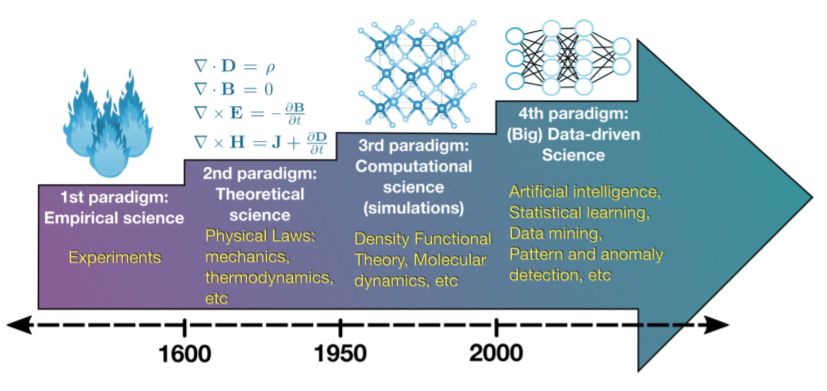
\includegraphics[width=0.6\textwidth]{figures/paradigms.png}
    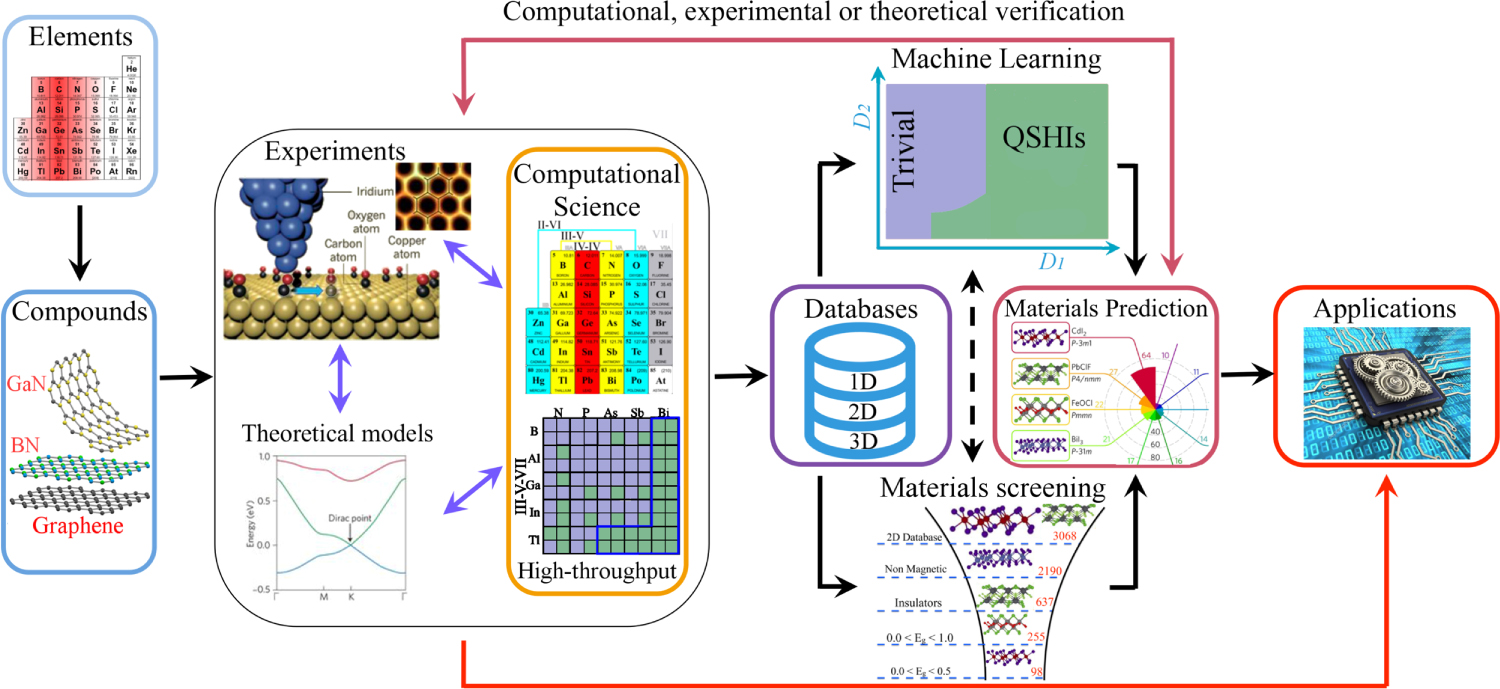
\includegraphics[width=0.9\textwidth]{figures/ht-workflow.jpg}
    \caption{[PLACEHOLDER] Schematic of an example workflow in material informatics. 
    %\marianne{Morten: can you please add the other schematic figure we discussed as placeholder? Sebastian makes our own versions of these schematic figures (I can make some VESTA files with materials). We should have just one figure I think, perhaps even combining the paradigms and explaining the material informatics worklow.} 
    }
    \label{fig:paradigm}
\end{figure}

Several platforms are available for the development of quantum technologies (QT) but the materials and fabrication technologies are less mature than those for, e.g., classical computers and sensors. 
An important concern in this context is that of scalability. 
For example, the best performing quantum computer prototypes available today rely on superconducting electronics or trapped ions. Both technologies require millikelvin temperatures to operate, fabrication is challenging, and the stability of interactions between qubits is an issue. Instead, semiconductors are emerging as a promising alternative platform, offering competitive characteristics combined with the possibility of room temperature operation and mature and scalable material processing and fabrication.  

Quantum technologies based on semiconductors rely on either defects or quantum dots where the latter kind can be of the self-assembled or fabricated type. 
Semiconductor defects can act as single-photon emitters or spin centers and are compatible with the three main QT categories of computing, communication and sensing.  
These characteristics are most often found for the case of defects that introduce deep energy levels into the semiconductor band gap. So-called deep level defects can trap carriers in localized states that are essentially isolated from the surroundings, making them highly suitable for QT due to, e.g., reliable single-photon emission and long spin coherence times. 
The most well-known QT defect is the negatively charged nitrogen-vacancy (NV) center in diamond \cite{Doherty_2013}, but silicon carbide (SiC) and the various quantum emitters therein are poised to out-compete diamond in certain areas due to the favorable emission wavelength region in the near infrared and telecom coupled with more mature material processing and fabrication  \cite{Bathen2021}. 
However, defect based QT is still in the early stages, and the issues left to address include identification of suitable host materials and candidate defects, and scalable and reproducible quantum device fabrication. Another important issue is that the understanding of the requirements for a material to enable quantum compatible properties to manifest remains lacking,  
%The plethora of possible emitters and spin centers formed by semiconductor defects or nanostructures come with different characteristics that are compatible with specific applications.  
%Additionally, the understanding of what exactly makes a semiconductor based quantum platform suitable for QT is scarce, 
and the selection of quantum compatible semiconductor host materials is slim. 

The majority of discoveries of quantum emitters in semiconductors has so far happened by serendipity, and there is an urgent need for 
%new and better materials that can escalate the effort for a sustainable future. 
a better understanding of how different materials properties manifest. 
In this context, a framework for dedicated materials search and analysis is needed. 
The fourth science paradigm of big data driven science presents a significant improvement over the third paradigm focusing on computational science, for instance via density functional theory calculations of different materials properties. The fourth paradigm 
%, as illustrated by the schematic in Figure~\ref{fig:paradigm}(a), 
introduces the potential of targeted search for promising material systems to act as hosts for qubit and single-photon emitter defects.  
Instead of searching through a host of signals for the one that matches our criteria, we are now able to \textit{predict} which materials and signatures we should target for more detailed studies. 
This is made feasible by the availability of databases containing material properties for a wide range of different systems. In this work, the data in question is provided by bulk density functional theory (DFT) calculations to obtain the ground state properties of different elements and compounds. Combined with machine learning algorithms we provide a path towards precise classification of qubit candidates. The inclusions of machine learning methods follows recent trends in applications of 
statistics, data science and machine learning for scientific discoveries, see for example Refs.~\cite{deiana2021,Carleo2019}.





In this work we provide a framework for the data mining and automated discovery of promising solid-state material hosts for quantum emitters and spin centers using targeted database search and machine learning methods combined with knowledge from the field. The methodology developed herein can be modified for other material types and application areas provided that a large enough database with relevant theoretical or experimental data is available. 
The method that was developed relies on data extraction from the databases Materials Project \cite{Jain2013,Jain2018}, The Open Quantum Materials Database (OQMD) \cite{Saal2013, Kirklin2015}, JARVIS-DFT \cite{Choudhary2020}, AFLOW \cite{Curtarolo2012, Curtarolo2012a, Calderon2015} and AFLOW-ML \cite{Isayev2017}. 
Matminer \cite{Ward2018} is then used for material analysis to featurize the extracted data. 
An important feature of the work is the database building and development of the training sets for the machine learning models. We have developed three different approaches to data mining: (i) \emph{the Ferrenti approach} which is similar to that proposed by \citeauthor{Ferrenti2020}  \cite{Ferrenti2020}, (ii) \emph{the augmented Ferrenti approach} and (iii) \emph{the insightful approach}. We find that the former two methodologies base their data extraction protocols on practical considerations, such as experimental availability in specific forms or the toxicity of the materials, leading to few observable trends in the materials predicted by well-tested machine learning algorithms, such as logistic regression, decision trees, and ensemble methods like random forests and gradient boosting \cite{mehta2019,hastie2009}. The third approach, on the other hand, relies on materials with experimentally proven advantageous characteristics in the training set. This more restricted approach proved more suitable than the other two and yielded $214$ predicted candidates with examples such as ZnGeP$_2$, MgSe, CdS, BP, BC$_2$N, BP, Ge, GeC, InP, and InAs. 
%\begin{itemize}
 %   \item Data was extracted from databases materials project ... 
 %   \item Featurization using matminer 
 %   \item Initial database building similar to Ferrenti et al \cite{Ferrenti2020}, but method is expanded to focus mainly on physical aspects. 
 %   \item Machine learning on top.  
%\end{itemize} 

%\section*{Theoretical Background and Experimental Data} 

%Quantum technologies, including sensing, communication and computing, are intriguing because of the new capabilities they offer. However, realization of large-scale fabrication for these techniques requires further technological development. The superconducting electronics platform that is currently employed for quantum computers necessitates millikelvin temperatures and may prove challenging to scale. Instead, recent developments have seen/heralded the rise of semiconductors as possible host materials for a variety of quantum devices. Semiconductor quantum dots or point defects could prove easier to combine with existing devices, and room temperature operation of prototype communication and computing devices has been shown.  However, this technology is still in the early stages, and the issues left to address include scalable and reproducible device fabrication, identification of ideally suited host candidates, and, importantly, understanding the requirements for a material to act as a good host remain unclear. 

%\subsection*{Semiconductors as a Quantum Host} 
%Quantum technologies commonly rely on a quantum bit or qubit as the basis for operation. \marianne{Some schematic is shown in Figure~\ref{fig:qt}}. For all applications, the basic requirement is a two-level quantum system which is essentially isolated from its environment, ensuring sufficient stability to perform various operation. In other words, we search for systems which exhibit a high degree of coherence. Additionally, the qubit state must be controlable via repeatable initialization, manipulation and read-out protocols. A set of requirements were formulated by DiVincenzo for the case of qubits and quantum computing \cite{DiVincenzo2000}. Below, these are rephrased to encompass qubit requirements for all three QT application areas:  
%\begin{itemize}
 %   \item A scalable physical system with well-characterized qubits
 %  \item Reliable qubit initialization protocols 
 %   \item Quantum gates and protocols to operate on and control qubit states  
 %   \item Qubit state coherence time must exceed gate operation time 
 %   \item Qubit state read-out after operation, preferably optically.  
%\end{itemize}

%\begin{figure}[t]
 %   \centering
 %   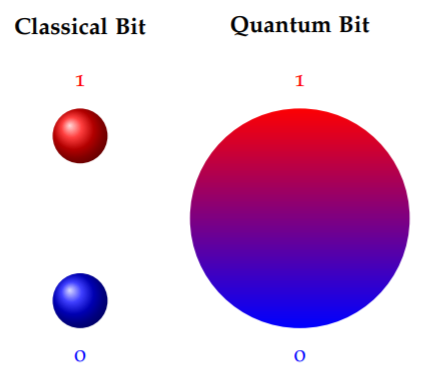
\includegraphics[width=0.3\textwidth]{figures/qubit.png}
 %   \caption{[PLACEHOLDER] Schematic of classical versus quantum bits. }
 %   \label{fig:qt}
%\end{figure}

%Discuss experimental data and the semiconductor platform. 
%Semiconductors embody point defects that may trap charge carriers, causing deep energy levels to appear within the fundamental band gap. Importantly, deep level defects can trap carriers in localized states that are essentially isolated from the surroundings, making them suitable for QT. A prime example is the nitrogen-vacancy (NV) center in diamond, which has been proposed as a contender for both computing, sensing and communication applications \cite{Doherty_2013}. The NV center is a room temperature single-photon source emitting in the visible portion of the spectrum, and has been employed for, e.g., stress tensor mapping \cite{Broadway2019} and optical imaging of living cells \cite{Lesage_2013}. Moreover, the NV center in its negative charge state traps an electron in a localized and high-spin $S=1$ state that can be coherently controlled and with RT spin coherence times above \SI{1}{\milli\second} \cite{Doherty_2013}, leading to demonstrations of entanglement and teleportation of two NV center spins \cite{Bernien2013,Pfaff_2014}. However, despite these promising discoveries, diamond  as a quantum platform comes with several important drawbacks. The relevant defects therein, such as the NV center, emit in the visible region of the spectrum which is not compatible with the telecom wavelengths needed to integrate with optical fiber technology. Additionally, diamond is expensive, device fabrication is challenging and scalability is poor, leading to concerns in whether quantum technology device development will be realizable on this platform. Hence, we search among the plethora of available semiconductors for a platform that can deliver on the necessary parameters for QT applications while also, ideally, providing availability and scalable fabrication. In this context, the material properties that facilitate quantum compatible characteristics such as single-photon emission and coherent spin manipulation to manifest must be identified. 

%\begin{figure}[t]
%    \centering
%    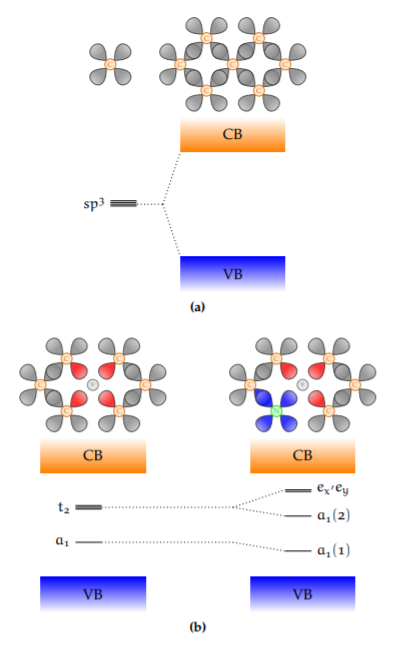
\includegraphics[width=0.5\textwidth]{figures/NV.png}
%    \caption{[PLACEHOLDER] Schematic representation of the electronic structure of the NV center in diamond.}
%    \label{fig:defects-dft}
%\end{figure}

%\begin{figure}[t]
 %   \centering
 %   \includegraphics[width=0.5\textwidth]{figures/defects-sic.pdf}
 %   \caption{[PLACEHOLDER] Schematic representation of different quantum compatible defects in SiC and the energy levels they introduce into the band gap, from Ref.\cite{Bathen2021}.} 
 %   \label{fig:defects-sic}
%\end{figure}

%Table \ref{tab:qt-materials} contains an overview of known semiconductor materials with demonstrated quantum compatible characteristics. In this context we consider single-photon emission and coherent spin manipulation for systems related to point defects primarily, but also self-assembled or lithographically structured quantum dots. \marianne{A (placeholder) schematic of quantum compatible defects and the energy levels they introduce into the band gap of 4H-SiC is shown in Figure~\ref{fig:defects-sic}.} Most of the defects in the table have yet to be identified, and different material related challenges complicate the implementation of defects for QT. A set of common denominators for materials that contain qubit defects was summarized by Weber et al. \cite{Weber2010}: 
%\begin{itemize}
 %   \item Wide band gap to facilitate localized deep levels (physical)
 %    \item Low spin orbit coupling to extend spin coherence times (physical) 
 %   \item Low el-phonon coupling for sharp emission lines (physical) 
 %   \item Availability as high-quality, bulk, or thin-film single crystals (practical)
 %   \item Constituent elements with naturally occurring isotopes of zero nuclear spin (practical). 
%\end{itemize}
%Note the division between physical and practical requirements in the list above. The physical criteria refer to some fundamental aspect of the material that permits specific properties to manifest, while practical refers to the external influences that simplify measurement and detection of the interesting properties. In this work, we will focus primarily on the former set of criteria, as understanding them better may give further insights into the makings of a reliable QT platform. 

%In addition to obtaining greater understanding of  exactly what constitutes a good quantum host material, we must recognize that different defect and material types may suit different needs. Therefore, we aim to develop a bigger bank of candidate defects and materials. So far, detection of QT compatibility in semiconductors has been rather slow, depending on signal detection and later identification in each specific material. Instead, we are looking for a top-down approach to \textit{predict} promising materials, enabling a guiding of experimental efforts. 

%\subsection*{Density Functional Theory Output} %Marianne 
%The density functional theory (DFT) is a versatile and powerful theoretical approach that has been exceptionally successful in predicting solid-state material properties such as stability of different phases, lattice parameters and band gaps. DFT provides a method for iteratively solving the Schr{\"o}dinger equation based on initial guesses for the atomic potentials. Using DFT calculations, we are able to accurately investigate semiconductor materials with many atoms while keeping efficiency and cost in mind.  

%The fundamental challenge of the DFT is that the calculations rely on approximations to the potential function of a system as expressed by the exchange-correlation (XC) functional, which is not known for bulk materials. The XC functional is usually grouped into three categories based on the level of theory. The local density approximation (LDA) takes the homogeneous electron gas as a starting point, while the more advanced general gradient approximation (GGA) includes also the gradient in local electron gas variations. These local or semi-local functionals yield satisfactory results on geometrical concerns but tend to underestimate energies such as the band gap or defect energy levels due to a self-interaction error (i.e., an electron is allowed to interact with itself) [Ref SchollSteckel] \cite{Freysoldt2014}. More recent developments have seen the widespread use of hybrid functionals such as the HSE06 incorporating a portion of Hartree-Fock exact exchange \cite{Heyd2003},  albeit at a much greater computational cost. 

%Despite the limitations imposed by the approximate nature of the XC functional, and the band gap error of LDA and GGA level functionals, DFT can be a powerful tool when predicting, designing and interpreting experiments. Herein, we employ databases containing DFT calculations of material properties to gain insight into the fundamental mechanisms behind observed quantum characteristics, and predict new candidate QT hosts. The calculations we employ were performed using the GGA-level Perdew-Burke-Erznerhof (PBE) functional \cite{Perdew1996}. Note that the PBE functional tends to underestimate the band gap of semiconductor materials. Nonetheless, a larger data set is available than for, e.g., HSE06, and many trends are conserved also with PBE. The ground-state (and $0$~K) parameters that can be extracted from this type of data set include the total energy (translates into stability), the band gap, the electronegativity, the electron-phonon coupling and magnetic properties. 

%\begin{figure}[t]
%    \centering
%    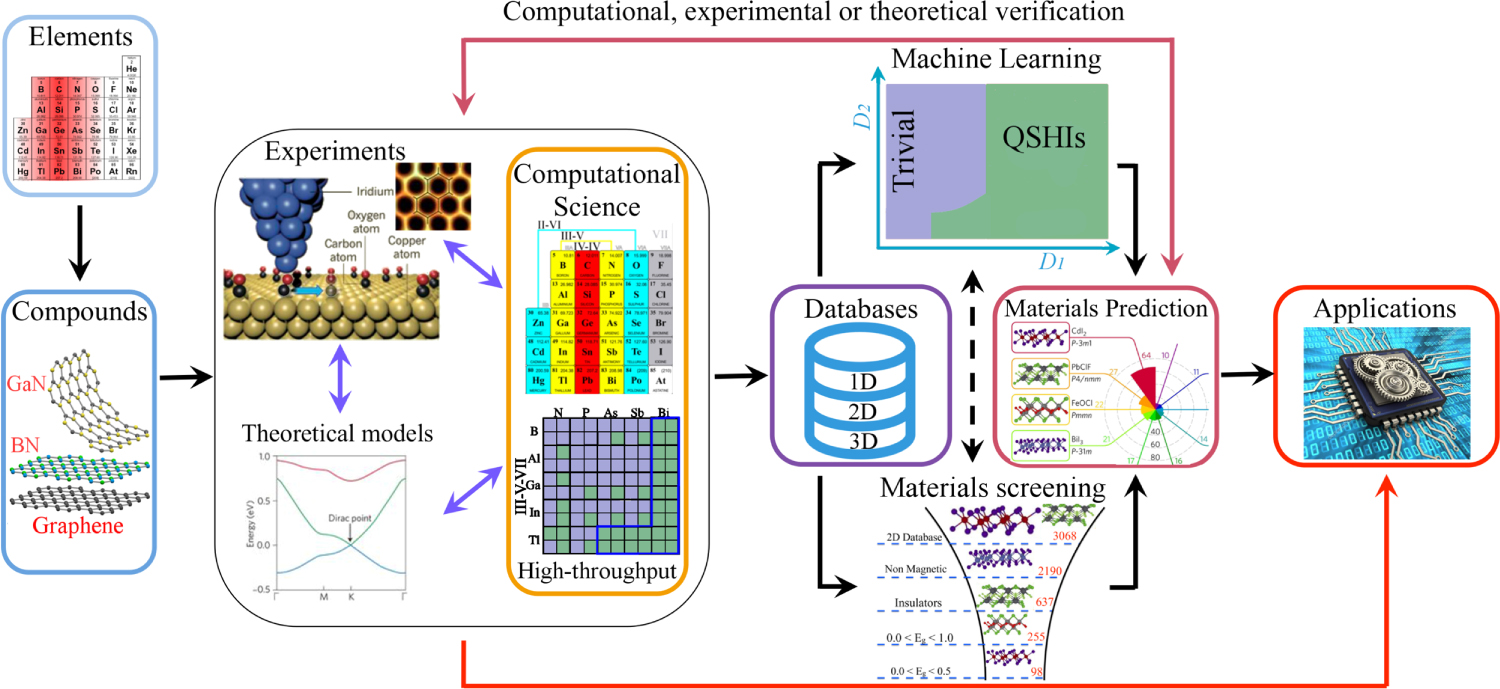
\includegraphics[width=\textwidth]{figures/ht-workflow.jpg}
%    \caption{[PLACEHOLDER for workflow] Morten: can you please add the other schematic figure we discussed as placeholder? Sebastian makes our own versions of these schematic figures (I can make some VESTA files with materials). }
%    \label{fig:ht-workflow}
%\end{figure}

%\subsection*{Machine Learning} 

%Should contain a brief description of the four ``algorithms'':
%\begin{itemize}
 %   \item Logistic regression
 %   \item Decision trees
 %   \item Random forest
 %   \item Gradient boost
%\end{itemize}

%Why these? Works well out of the box, I guess. Readily available in scikit-learn.

\section*{Results and discussion}
%Includes discussion of results. 

\subsection*{Information Flow}  %Sebastian/Oliver (Marianne) 
% MEB: Since Methods are at the end, I propose to put part of this
% discussion in the Results section. 
% This is because it is an important result of the work, and also
% because it is important to understand the rest of the paper 

The information stream in this work can be regarded as many
modular parts connected in logical pieces. The initial step for
gathering material data and building features is visualized by the
the flowchart in Figure~\ref{fig:flowchart-makedata}. 
Initially, we start by extracting all entries in
the Materials Project that matches a specific query. 

\setlength{\abovecaptionskip}{5cm}
\begin{figure}[!ht]
\begin{picture}(20,10)

\setlength{\unitlength}{0.17in}
\put(-15,-5){\framebox(7,3){Initial MP query}}
\put(-8,-3.5){\vector(3,0){2}}
\put(-6,-3.5){\line(0,3){3}}
\put(-6,-3.5){\line(0,-3){3}}
\put(-6,-6.5){\line(1,0){17}}

\put(-1.5,-5){\framebox(3.5,2){AFLOW}}
\put(0.24,-5){\vector(0,-1){1.5}}

\put(3,-5){\framebox(5,2){AFLOW-ML}}
\put(5.5,-5){\vector(0,-1){1.5}}

\put(-3,-10){\framebox(3,2){OQMD}}
\put(-2.5,-8){\vector(0,1){1.5}}

\put(1,-10){\framebox(5,2){JARVIS-DFT}}
\put(3.5,-8){\vector(0,1){1.5}}

\put(7,-10){\framebox(2,2){CI}}
\put(8,-8){\vector(0,1){1.5}}

\put(-6,-0.5){\vector(1,0){5}}
\put(-1,-1.5){\framebox(8,2){Matminer featurizer}}
\put(7,-0.5){\line(1,0){4}}

\put(11,-0.5){\vector(0,-1){3}}
\put(11,-6.5){\vector(0,1){3}}

\put(11,-3.5){\vector(1,0){2}}
\put(13,-4.5){\framebox(6,2){interim data}}

\end{picture}
\caption{The data flow of the main project, starting from an initial MP-query, and ending with a featurized dataset with entries from several other databases. The matminer featurizer step is further visualized in-depth in Figure \ref{fig:flowchart-featurization}.}
\label{fig:flowchart-makedata}
\end{figure}
%\vskip0cm
%\setlength{\abovecaptionskip}{0cm}


\setlength{\abovecaptionskip}{10cm}
\begin{figure}[!ht]
\begin{picture}(20,20)
\setlength{\unitlength}{0.17in}

%\put(13.5, 0.5){\makebox{\thead{\textbf{Matminer featurizer}}}}
%\put(0.,-22){\framebox(33.5,22){\thead{}}}

\put(-16,-8.5){\vector(1,0){2.5}}
\put(-13.5,-10.5){\framebox(4,4){\thead{Partition \\ dataset}}}
\put(-9.5,-8.5){\vector(3,0){2}}
\put(-7.5,-10.5){\framebox(5,4){\thead{Get objects \\ from MP}}}
\put(-2.5,-8.5){\line(3,0){1}}
\put(-1.5,-8.5){\line(0,1){6}}
\put(-1.5,-8.5){\line(0,-1){6}}

\put(-1.5,-2.5){\vector(3,0){1}}
\put(-0.5,-3.5){\framebox(9,2){Featurize composition}}
\put(8.5,-2.5){\line(3,0){1}}

\put(-1.5,-5.5){\vector(3,0){1}}
\put(-0.5,-6.5){\framebox(9,2){Featurize structure}}
\put(8.5,-5.5){\line(3,0){1}}

\put(-1.5,-8.5){\vector(3,0){1}}
\put(-0.5,-9.5){\framebox(9,2){Featurize site}}
\put(8.5,-8.5){\line(3,0){1}}

\put(-1.5,-11.5){\vector(3,0){1}}
\put(-0.5,-12.5){\framebox(9,2){Featurize dos}}
\put(8.5,-11.5){\line(3,0){1}}

\put(-1.5,-14.5){\vector(3,0){1}}
\put(-0.5,-15.5){\framebox(9,2){Featurize band}}
\put(8.5,-14.5){\line(3,0){1}}

\put(9.5,-8.5){\line(0,1){6}}
\put(9.5,-8.5){\line(0,-1){6}}

\put(9.5,-8.5){\vector(2,0){1}}
\put(10.5,-10.5){\framebox(5.5,4){\thead{Done with \\ all partitions?}}}

\put(14, -12.){\makebox{NO}}
\put(13.5,-10.5){\line(0,-1){8}}
\put(13.5,-18.5){\vector(-1,0){16}}
\put(-7.5,-20.5){\framebox(5,4){\thead{Select next \\ partition}}}
\put(-5,-16.5){\vector(0,1){6}}


\put(16, -8.5){\vector(1,0){3.5}}
\put(16.5, -8.){\makebox{YES}}

\end{picture}
\caption{The process of the matminer featurizer step.  
%as seen in Figure \ref{fig:flowchart-makedata}. 
To limit the memory and computational usage, the data is partitioned into smaller subsets where the respective pymatgen objects are obtained through a query to be used in the following featurization steps. This process is repeated iteratively until all the data has been featurized. Abbreviations used are Materials Project (MP), density of states (DOS) and electronic band structure (band).}
\label{fig:flowchart-featurization}
\end{figure}
%\vskip15cm
%\setlength{\abovecaptionskip}{10cm}


Thereafter, we apply Matminer’s \cite{Ward2018}
featurization tools to make thousands of features of the data. The conditions for this initial query are that the materials must derive from experimental data, and have a band gap wider than $0.1$~eV. In a parallel step, entries that are deemed
similar to the entries from the initial query
are extracted from 
OQMD \cite{Saal2013,Kirklin2015}, JARVIS-DFT \cite{Choudhary2020}, 
AFLOW \cite{Curtarolo2012, Curtarolo2012a, Calderon2015}, 
AFLOW-ML \cite{Isayev2017},
and
Citrine Informatics REF!??. The results of these steps are combined into
a data set for further analysis.

A schematic describing the featurization process in Matminer is shown in Figure~\ref{fig:flowchart-featurization}. 
\textbf{[Describe it and say something about which features we choose.]}  
The 39 features selected in this work are summarized in the Supplementary Material at \cite{supplementary}. 


\subsection*{Data Mining}

After compiling a dataset from the procedure outlined above, we 
face a challenge in terms of defining a training set that %we can train data on. 
can be used to train an ML algorithm. 
This is challenging for two reasons. 
Firstly, although defects like the NV center in diamond and emitters in SiC are becoming
increasingly well studied, few candidate materials are known. An additional consideration
is that the physical mechanisms promoting favorable defect properties are not fully understood. 
Secondly, defining materials as unsuitable candidates for QT has proven to be surprisingly
intricate. 
%This is not only challenging due to the lack of known suitable candidates (1),  but also due to the intricacy of defining materials as unsuitable candidates (0). 
We follow three separate procedures to define a training set consisting of both suitable and unsuitable material candidates for QT. 

\subsubsection*{The Ferrenti approach}

The first approach to defining a training set is based on the criteria
from the paper by \citeauthor{Ferrenti2020} \cite{Ferrenti2020}.
They suggest a data mining process consisting of four stages by 
systematically evaluating the suitability of host materials from
the Materials Project. 

In this framework, we label \textbf{suitable} candidates by the following steps. 
\begin{enumerate}
    \item Include materials that;
    \begin{itemize}
        \item contain elements with more than $50\%$ natural abundance of 
            zero spin isotopes,
        \item crystallize in non-polar space groups,
        \item are present in the ICSD database, and
        \item are calculated to be nonmagnetic. 
    \end{itemize}
    \item Pragmatically remove toxic, radioactive and otherwise 
        ``difficult'' materials;
    \begin{itemize}
        \item exclude Th, U, Cd and Hg,
        \item exclude any rare-earth metals and noble gases,
        \item exclude Ru, Os, Fe or Ni.
    \end{itemize}
    \item Include only materials with a band gap larger than $0.5$~eV calculated using DFT and the PBE functional. 
    \item Ensure that energy above hull is less than $0.2$~eV per atom.
\end{enumerate}

We then label \textbf{unsuitable} candidates as materials in the ICSD database that crystallize in polar space groups, are calculated 
to be magnetic and have a band gap larger than $0.1$~eV as calculated by PBE-GGA.

\subsubsection*{The augmented Ferrenti approach}
In the second approach, we adjust the first approach in order to 
improve the dataset. This approach is therefore named
\emph{the augmented Ferrenti approach}.

In the first approach we included criteria that were not physically motivated, but instead based on a purely practical perspective, like excluding toxic and
radioactive elements. Such criteria are not necessarily related to what makes 
a material suitable for quantum technology - eventually it is up to the 
experimentalist to decide the practicality of the material to be employed. 
Consequently, in the augmented Ferrenti approach, we remove stage two from the approach above. What is more, we will include a few additional elements that have shown promising properties, but were initially excluded due to the lack of spin zero isotopes. 

The following steps make up the process of choosing \textbf{suitable} candidates 
in the \emph{augmented Ferrenti approach},
\begin{enumerate}
    \item Include materials that; 
    \begin{itemize}
        \item contain elements where more than half have a natural abundance of zero spin isotopes, except Al, P, Ga, As, B and N, 
        \item crystallize in non-polar space groups,
        \item are present in the ICSD database,
        \item are calculated to be nonmagnetic. 
    \end{itemize}
    \item Only keep materials that have a band gap larger than $1.5$~eV as calculated by PBE-GGA,
    \item Ensure energy above hull is less than $0.2$~eV per atom. 
\end{enumerate}

For \textbf{unsuitable} candidates, we implement the same strategy as the non-augmented
Ferrenti approach. The result is a somewhat unbalanced dataset, with up to $75 \ \%$ of the 
materials found in the suitable group. However, the dataset is $78 \ \%$ larger than for
the Ferrenti approach.

\subsubsection*{The insightful approach}
The third approach differs substantially from the first two approaches in terms 
of labeling, as we apply knowledge from the field (see for instance Refs.~\cite{Atatuere2018,Zhang2020,Son2020,Toth2019,Bathen2021} for an overview)   
to pick our promising material host candidates. We therefore name this scheme 
\emph{the insightful approach}. 
Due to the concern of having an insufficient dataset, we will include
materials that are promising and have shown suitable properties to 
accommodate deep defects that potentially can exhibit quantum effects. 
Materials where properties like single-photon emission and spin manipulation are attributed to quantum dot self-assembled formation or lithographic structuring will also be included in this context.  
The approach to pick \textbf{suitable} candidates can be summed up as;   
\begin{enumerate}
    \item Pick candidates that match the formulas in Table~\ref{tab:qt-materials}, or the formulas ZnSe,  AlP, GaP, AlAs, ZnTe, CdS \cite{Weber2010} or SiGe \cite{Hardy2019}. 
    \item Make sure the candidates are present in the ICSD database.  
    \item Perform a manual screening for correct structures.
\end{enumerate}

\begin{table}[b]
    \centering 
    \caption{Overview of materials and defects that have been demonstrated to exhibit QT compatible characteristics such as single-photon emission and coherent spin manipulation.}
    \begin{tabular}{c|c|c|c}
    Material & Band gap (eV) & Defect candidates & References \\
    \hline
    Diamond  & $5.5$  & N$_\mathrm{C}V_\mathrm{C}$, Si$_\mathrm{C}V_\mathrm{C}$, Ge$_\mathrm{C}V_\mathrm{C}$ & \cite{Taylor2008,Balasubramanian_2009,Barclay2011,Gordon2013,Rogers_2014,Bhaskar_2018} \\ 
    SiC & $2.2$-$3.3$ & $V_\mathrm{Si}$, $V_\mathrm{Si}V_\mathrm{C}$, C$_\mathrm{Si}V_\mathrm{C}$, N$_\mathrm{C}V_\mathrm{Si}$ & \cite{Widmann2014,Christle_2015,Castelletto_2014,Zargaleh_2018}  \cite{Weber2010, Son2020, Falk2013} \\ 
    Si & $1.1$ & P, G, unidentified & \cite{Muhonen_2014,Durand_2020,Redjem2020} \\ 
    (2D) \textit{h}-BN & $6.0$ & Unidentified defects & \cite{Tran_2016,Tran_2016b,Hayee_2020} \\ 
    (2D) MoS$_2$, WSe$_2$, WS$_2$ & $<2.5$~eV & Bound excitons & \cite{Toth2019} \\
    ZnO & $3.4$ & Unidentified defects & \cite{Morfa2012} \\ 
    ZnS & $3.6$ (zincblende) & Unidentified defects & \cite{Stewart2019} \\ 
    GaAs & $1.4$ & Quantum dots & \cite{Bluhm2010} \\ 
    GaN & $3.4$ & Quantum dots, unidentified defects & \cite{Roux2017,Berhane2018} \\
    AlN & $6.0$ & Unidentified defects & \cite{Xue2020}\\
    \end{tabular}
    \label{tab:qt-materials}
\end{table} 

Table~\ref{tab:qt-materials} contains an overview of known semiconductor materials with demonstrated quantum compatible characteristics. In this context, we consider single-photon emission and coherent spin manipulation.   
The table forms the basis for picking suitable candidates for the insightful approach. 
The properties being studied arise from mechanisms related to, e.g., point defects, excitons, and both self-assembled and lithographically structures quantum dots. 
Quantum emission signatures have been assigned to specific defects in diamond and SiC, but for most other materials, identification of the responsible defects still remains. 
In the insightful approach, we include materials that are known to be quantum compatible as outlined in Table~\ref{tab:qt-materials} in the training set, but also the materials ZnSe, AlP, GaP, AlAs, ZnTe, CdS and SiGe that have been predicted to act as good quantum hosts based on favorable properties such as wide band gap and low spin-orbit coupling \cite{Weber2010,Hardy2019}. 

After the first stage of picking candidates we are left with a list of 202 matching formulas which include 12 entries that have a band gap of less than $0.4$~eV. These structures are unstable in terms of energy above hull calculations, and will decompose into other materials in the list with a band gap that is substantially above $0.5$~eV. We include all of these structures except for C (mp-568410) having a PBE-computed band gap of $0.12$~eV - a metal according to AFLOW-ML and therefore labeled as an unsuitable candidate. 
 
%% OH: Dirty details about suitable materials:
Entries matching the formula C, SiC, BN, MoS$_2$, WSe$_2$ and WS$_2$ were manually screened to see if the entries have a matching structure to the respective candidates discussed earlier. %OH: Is discussed earlier in thesis but maybe neccessary to mention here? 
For C, we admit three-dimensional diamond-like structures as explicitly stated in the column tags at Materials Project. Additionally, we find many two-dimensional structures of carbon with a large band gap ($>1.5$ eV) in the data. We add these as suitable candidates. Complex structures (eg. C$_{28}$, C$_{48}$, C$_{60}$) were moved to the test set. For SiC, we admitted all entries, which involved $2$H, $3$C, $4$H, $6$H and $15$R. Concerning BN, MoS$_2$, WSe$_2$ and  WS$_2$, we only admit two-dimensional structures. For non-matching structures not mentioned so far, we move them to the test set to see if they will be predicted suitable or not by the models in a later step.

The materials AlP, GaP, AlAs, ZnTe and CdS were manually screened for tetrahedrally coordinated structures, and have been included since \citeauthor{Weber2010} \cite{Weber2010} has identified them as potentially promising candidates due to acceptable properties defined in requirements (H1-H4) in \autoref{ssec:qubit-material-host-requirements}. We note that only tetrahedrally coordinated structures of the given formulas were present after the band gap restriction of $0.5eV$.

The suitable candidates contain only compounds that are either elementary (unary) or binary. We do not want to discriminate based on the number of elements in a compound, therefore we remove the feature that describes the number of elements in a compound. After three stages, a total of $187$ entries were labeled as suitable candidates.
%% OH: Stop details suitable materials

Since the dataset constituting suitable candidates in the third approach contains few entries, we add 400 \emph{unsuitable}
candidates. These are picked at random from the pool of unsuitable candidates 
from the two previous approaches, in addition to those that are marked as unsuitable through
the manual screening process. 
See the Supplementary Material at \cite{supplementary} for a table containing the manually screened materials that were labeled as suitable candidates in the training set for the insightful approach. 


\subsubsection*{Comparing the approaches}

The three different methods for data mining place a particular emphasis on each of their particular goals. The Ferrenti approach depends on choosing only elements with zero spin isotopes together with practical filters, while the augmented Ferrenti approach allows a larger variety of elements and removes the practical reasons for excluding elements. Thus, the first approach targets a more narrow prediction space than the second approach does. However, perhaps the most restricted approach is the insightful approach. Since the variety of known suitable materials is substantially more restricted than for the two other approaches, we would expect the insightful approach to provide an even narrower prediction space. 
\textbf{[Are there any pros or cons we could mention on narrow prediction spaces?]}

%\marianne{Short paragraph here (or somewhere else) highlighting the potential issues with the two first approaches in terms of actually identifying any trends.}

We provide a visualization of each approach's training data as a parallel coordinate plot for a few selected features in Figure~\ref{fig:parallel-coordinates-approaches}. Parallel coordinate schemes \cite{Inselberga1990, Inselberg1985} represent a multi-dimensional data tuple as one polyline crossing a parallel axis. The selected features are found on the x-axis, while the y-axis shows the value of the data present. Thus, parallel coordinate plots can turn many-dimensional data into a compact two-dimensional representation. Due to possible data cluttering, the figure visualizes a random sample of each class with an upper limit of $250$ per class with transparent lines. The green and red polylines represent suitable and unsuitable candidates, respectively. 

The Ferrenti approach and the augmented Ferrenti approach share similarities; 
for example, all unsuitable candidates exhibit polar space groups, and their upper limits for both ionic character and covalent range are equal for suitable candidates.  
%such as having only unsuitable candidates with polar space groups and having an equal amount of upper limit for both ionic character and covalent range for suitable characters. 
Additionally, the two approaches share that suitable candidates can consist of up to five different elements. 
Interestingly, we observe that
the entries in Fig.~\ref{fig:parallel-coordinates-approaches} span the same dimensions for the Ferrenti and augmented Ferrenti approaches, despite the more restricted nature of the former. 
%even if the augmented Ferrenti approach is less restricted, it appears that the entries span the same dimensions.

The biggest difference is found for the insightful approach. The entries selected as suitable candidates do not exhibit any magnetization, even though there are both polar and non-polar space groups present. Additionally, the range of covalent radius and maximum ionic character span a substantially smaller space than the Ferrenti-based approaches. 
\textbf{This can be interpreted as ... }

\begin{figure}[t] %!htp
    \centering
    \begin{subfigure}{1\textwidth}
        \centering
          %% Creator: Matplotlib, PGF backend
%%
%% To include the figure in your LaTeX document, write
%%   \input{<filename>.pgf}
%%
%% Make sure the required packages are loaded in your preamble
%%   \usepackage{pgf}
%%
%% and, on pdftex
%%   \usepackage[utf8]{inputenc}\DeclareUnicodeCharacter{2212}{-}
%%
%% or, on luatex and xetex
%%   \usepackage{unicode-math}
%%
%% Figures using additional raster images can only be included by \input if
%% they are in the same directory as the main LaTeX file. For loading figures
%% from other directories you can use the `import` package
%%   \usepackage{import}
%%
%% and then include the figures with
%%   \import{<path to file>}{<filename>.pgf}
%%
%% Matplotlib used the following preamble
%%   \usepackage[detect-all,locale=DE]{siunitx} \usepackage[T1]{fontenc} \usepackage[utf8x]{inputenc}
%%
\begingroup%
\makeatletter%
\begin{pgfpicture}%
\pgfpathrectangle{\pgfpointorigin}{\pgfqpoint{5.584422in}{2.192266in}}%
\pgfusepath{use as bounding box, clip}%
\begin{pgfscope}%
\pgfsetbuttcap%
\pgfsetmiterjoin%
\pgfsetlinewidth{0.000000pt}%
\definecolor{currentstroke}{rgb}{1.000000,1.000000,1.000000}%
\pgfsetstrokecolor{currentstroke}%
\pgfsetstrokeopacity{0.000000}%
\pgfsetdash{}{0pt}%
\pgfpathmoveto{\pgfqpoint{0.000000in}{0.000000in}}%
\pgfpathlineto{\pgfqpoint{5.584422in}{0.000000in}}%
\pgfpathlineto{\pgfqpoint{5.584422in}{2.192266in}}%
\pgfpathlineto{\pgfqpoint{0.000000in}{2.192266in}}%
\pgfpathclose%
\pgfusepath{}%
\end{pgfscope}%
\begin{pgfscope}%
\pgfsetbuttcap%
\pgfsetmiterjoin%
\definecolor{currentfill}{rgb}{1.000000,1.000000,1.000000}%
\pgfsetfillcolor{currentfill}%
\pgfsetlinewidth{0.000000pt}%
\definecolor{currentstroke}{rgb}{0.000000,0.000000,0.000000}%
\pgfsetstrokecolor{currentstroke}%
\pgfsetstrokeopacity{0.000000}%
\pgfsetdash{}{0pt}%
\pgfpathmoveto{\pgfqpoint{0.315279in}{0.114336in}}%
\pgfpathlineto{\pgfqpoint{5.263604in}{0.114336in}}%
\pgfpathlineto{\pgfqpoint{5.263604in}{1.609458in}}%
\pgfpathlineto{\pgfqpoint{0.315279in}{1.609458in}}%
\pgfpathclose%
\pgfusepath{fill}%
\end{pgfscope}%
\begin{pgfscope}%
\pgfpathrectangle{\pgfqpoint{0.315279in}{0.114336in}}{\pgfqpoint{4.948324in}{1.495122in}}%
\pgfusepath{clip}%
\pgfsetbuttcap%
\pgfsetmiterjoin%
\pgfsetlinewidth{0.501875pt}%
\definecolor{currentstroke}{rgb}{1.000000,0.388235,0.278431}%
\pgfsetstrokecolor{currentstroke}%
\pgfsetstrokeopacity{0.200000}%
\pgfsetdash{}{0pt}%
\pgfpathmoveto{\pgfqpoint{0.315279in}{0.182296in}}%
\pgfpathcurveto{\pgfqpoint{0.645168in}{0.182296in}}{\pgfqpoint{0.975056in}{1.541498in}}{\pgfqpoint{1.304944in}{1.541498in}}%
\pgfpathcurveto{\pgfqpoint{1.634833in}{1.541498in}}{\pgfqpoint{1.964721in}{1.332450in}}{\pgfqpoint{2.294609in}{1.332450in}}%
\pgfpathcurveto{\pgfqpoint{2.624497in}{1.332450in}}{\pgfqpoint{2.954386in}{0.648126in}}{\pgfqpoint{3.284274in}{0.648126in}}%
\pgfpathcurveto{\pgfqpoint{3.614162in}{0.648126in}}{\pgfqpoint{3.944051in}{0.764811in}}{\pgfqpoint{4.273939in}{0.764811in}}%
\pgfpathcurveto{\pgfqpoint{4.603827in}{0.764811in}}{\pgfqpoint{4.933715in}{0.644335in}}{\pgfqpoint{5.263604in}{0.644335in}}%
\pgfusepath{stroke}%
\end{pgfscope}%
\begin{pgfscope}%
\pgfpathrectangle{\pgfqpoint{0.315279in}{0.114336in}}{\pgfqpoint{4.948324in}{1.495122in}}%
\pgfusepath{clip}%
\pgfsetbuttcap%
\pgfsetmiterjoin%
\pgfsetlinewidth{0.501875pt}%
\definecolor{currentstroke}{rgb}{1.000000,0.388235,0.278431}%
\pgfsetstrokecolor{currentstroke}%
\pgfsetstrokeopacity{0.200000}%
\pgfsetdash{}{0pt}%
\pgfpathmoveto{\pgfqpoint{0.315279in}{0.182296in}}%
\pgfpathcurveto{\pgfqpoint{0.645168in}{0.182296in}}{\pgfqpoint{0.975056in}{1.541498in}}{\pgfqpoint{1.304944in}{1.541498in}}%
\pgfpathcurveto{\pgfqpoint{1.634833in}{1.541498in}}{\pgfqpoint{1.964721in}{1.282126in}}{\pgfqpoint{2.294609in}{1.282126in}}%
\pgfpathcurveto{\pgfqpoint{2.624497in}{1.282126in}}{\pgfqpoint{2.954386in}{0.826800in}}{\pgfqpoint{3.284274in}{0.826800in}}%
\pgfpathcurveto{\pgfqpoint{3.614162in}{0.826800in}}{\pgfqpoint{3.944051in}{0.570639in}}{\pgfqpoint{4.273939in}{0.570639in}}%
\pgfpathcurveto{\pgfqpoint{4.603827in}{0.570639in}}{\pgfqpoint{4.933715in}{0.195962in}}{\pgfqpoint{5.263604in}{0.195962in}}%
\pgfusepath{stroke}%
\end{pgfscope}%
\begin{pgfscope}%
\pgfpathrectangle{\pgfqpoint{0.315279in}{0.114336in}}{\pgfqpoint{4.948324in}{1.495122in}}%
\pgfusepath{clip}%
\pgfsetbuttcap%
\pgfsetmiterjoin%
\pgfsetlinewidth{0.501875pt}%
\definecolor{currentstroke}{rgb}{1.000000,0.388235,0.278431}%
\pgfsetstrokecolor{currentstroke}%
\pgfsetstrokeopacity{0.200000}%
\pgfsetdash{}{0pt}%
\pgfpathmoveto{\pgfqpoint{0.315279in}{0.216230in}}%
\pgfpathcurveto{\pgfqpoint{0.645168in}{0.216230in}}{\pgfqpoint{0.975056in}{1.541498in}}{\pgfqpoint{1.304944in}{1.541498in}}%
\pgfpathcurveto{\pgfqpoint{1.634833in}{1.541498in}}{\pgfqpoint{1.964721in}{0.485842in}}{\pgfqpoint{2.294609in}{0.485842in}}%
\pgfpathcurveto{\pgfqpoint{2.624497in}{0.485842in}}{\pgfqpoint{2.954386in}{0.616220in}}{\pgfqpoint{3.284274in}{0.616220in}}%
\pgfpathcurveto{\pgfqpoint{3.614162in}{0.616220in}}{\pgfqpoint{3.944051in}{0.570639in}}{\pgfqpoint{4.273939in}{0.570639in}}%
\pgfpathcurveto{\pgfqpoint{4.603827in}{0.570639in}}{\pgfqpoint{4.933715in}{0.260421in}}{\pgfqpoint{5.263604in}{0.260421in}}%
\pgfusepath{stroke}%
\end{pgfscope}%
\begin{pgfscope}%
\pgfpathrectangle{\pgfqpoint{0.315279in}{0.114336in}}{\pgfqpoint{4.948324in}{1.495122in}}%
\pgfusepath{clip}%
\pgfsetbuttcap%
\pgfsetmiterjoin%
\pgfsetlinewidth{0.501875pt}%
\definecolor{currentstroke}{rgb}{1.000000,0.388235,0.278431}%
\pgfsetstrokecolor{currentstroke}%
\pgfsetstrokeopacity{0.200000}%
\pgfsetdash{}{0pt}%
\pgfpathmoveto{\pgfqpoint{0.315279in}{0.182639in}}%
\pgfpathcurveto{\pgfqpoint{0.645168in}{0.182639in}}{\pgfqpoint{0.975056in}{1.541498in}}{\pgfqpoint{1.304944in}{1.541498in}}%
\pgfpathcurveto{\pgfqpoint{1.634833in}{1.541498in}}{\pgfqpoint{1.964721in}{1.367087in}}{\pgfqpoint{2.294609in}{1.367087in}}%
\pgfpathcurveto{\pgfqpoint{2.624497in}{1.367087in}}{\pgfqpoint{2.954386in}{1.133099in}}{\pgfqpoint{3.284274in}{1.133099in}}%
\pgfpathcurveto{\pgfqpoint{3.614162in}{1.133099in}}{\pgfqpoint{3.944051in}{0.764811in}}{\pgfqpoint{4.273939in}{0.764811in}}%
\pgfpathcurveto{\pgfqpoint{4.603827in}{0.764811in}}{\pgfqpoint{4.933715in}{0.252856in}}{\pgfqpoint{5.263604in}{0.252856in}}%
\pgfusepath{stroke}%
\end{pgfscope}%
\begin{pgfscope}%
\pgfpathrectangle{\pgfqpoint{0.315279in}{0.114336in}}{\pgfqpoint{4.948324in}{1.495122in}}%
\pgfusepath{clip}%
\pgfsetbuttcap%
\pgfsetmiterjoin%
\pgfsetlinewidth{0.501875pt}%
\definecolor{currentstroke}{rgb}{1.000000,0.388235,0.278431}%
\pgfsetstrokecolor{currentstroke}%
\pgfsetstrokeopacity{0.200000}%
\pgfsetdash{}{0pt}%
\pgfpathmoveto{\pgfqpoint{0.315279in}{0.266960in}}%
\pgfpathcurveto{\pgfqpoint{0.645168in}{0.266960in}}{\pgfqpoint{0.975056in}{1.541498in}}{\pgfqpoint{1.304944in}{1.541498in}}%
\pgfpathcurveto{\pgfqpoint{1.634833in}{1.541498in}}{\pgfqpoint{1.964721in}{1.053448in}}{\pgfqpoint{2.294609in}{1.053448in}}%
\pgfpathcurveto{\pgfqpoint{2.624497in}{1.053448in}}{\pgfqpoint{2.954386in}{0.871469in}}{\pgfqpoint{3.284274in}{0.871469in}}%
\pgfpathcurveto{\pgfqpoint{3.614162in}{0.871469in}}{\pgfqpoint{3.944051in}{0.958983in}}{\pgfqpoint{4.273939in}{0.958983in}}%
\pgfpathcurveto{\pgfqpoint{4.603827in}{0.958983in}}{\pgfqpoint{4.933715in}{0.812219in}}{\pgfqpoint{5.263604in}{0.812219in}}%
\pgfusepath{stroke}%
\end{pgfscope}%
\begin{pgfscope}%
\pgfpathrectangle{\pgfqpoint{0.315279in}{0.114336in}}{\pgfqpoint{4.948324in}{1.495122in}}%
\pgfusepath{clip}%
\pgfsetbuttcap%
\pgfsetmiterjoin%
\pgfsetlinewidth{0.501875pt}%
\definecolor{currentstroke}{rgb}{1.000000,0.388235,0.278431}%
\pgfsetstrokecolor{currentstroke}%
\pgfsetstrokeopacity{0.200000}%
\pgfsetdash{}{0pt}%
\pgfpathmoveto{\pgfqpoint{0.315279in}{0.233056in}}%
\pgfpathcurveto{\pgfqpoint{0.645168in}{0.233056in}}{\pgfqpoint{0.975056in}{1.541498in}}{\pgfqpoint{1.304944in}{1.541498in}}%
\pgfpathcurveto{\pgfqpoint{1.634833in}{1.541498in}}{\pgfqpoint{1.964721in}{1.367087in}}{\pgfqpoint{2.294609in}{1.367087in}}%
\pgfpathcurveto{\pgfqpoint{2.624497in}{1.367087in}}{\pgfqpoint{2.954386in}{1.133099in}}{\pgfqpoint{3.284274in}{1.133099in}}%
\pgfpathcurveto{\pgfqpoint{3.614162in}{1.133099in}}{\pgfqpoint{3.944051in}{0.764811in}}{\pgfqpoint{4.273939in}{0.764811in}}%
\pgfpathcurveto{\pgfqpoint{4.603827in}{0.764811in}}{\pgfqpoint{4.933715in}{0.837386in}}{\pgfqpoint{5.263604in}{0.837386in}}%
\pgfusepath{stroke}%
\end{pgfscope}%
\begin{pgfscope}%
\pgfpathrectangle{\pgfqpoint{0.315279in}{0.114336in}}{\pgfqpoint{4.948324in}{1.495122in}}%
\pgfusepath{clip}%
\pgfsetbuttcap%
\pgfsetmiterjoin%
\pgfsetlinewidth{0.501875pt}%
\definecolor{currentstroke}{rgb}{1.000000,0.388235,0.278431}%
\pgfsetstrokecolor{currentstroke}%
\pgfsetstrokeopacity{0.200000}%
\pgfsetdash{}{0pt}%
\pgfpathmoveto{\pgfqpoint{0.315279in}{0.267375in}}%
\pgfpathcurveto{\pgfqpoint{0.645168in}{0.267375in}}{\pgfqpoint{0.975056in}{1.541498in}}{\pgfqpoint{1.304944in}{1.541498in}}%
\pgfpathcurveto{\pgfqpoint{1.634833in}{1.541498in}}{\pgfqpoint{1.964721in}{0.678043in}}{\pgfqpoint{2.294609in}{0.678043in}}%
\pgfpathcurveto{\pgfqpoint{2.624497in}{0.678043in}}{\pgfqpoint{2.954386in}{0.597076in}}{\pgfqpoint{3.284274in}{0.597076in}}%
\pgfpathcurveto{\pgfqpoint{3.614162in}{0.597076in}}{\pgfqpoint{3.944051in}{0.570639in}}{\pgfqpoint{4.273939in}{0.570639in}}%
\pgfpathcurveto{\pgfqpoint{4.603827in}{0.570639in}}{\pgfqpoint{4.933715in}{0.469499in}}{\pgfqpoint{5.263604in}{0.469499in}}%
\pgfusepath{stroke}%
\end{pgfscope}%
\begin{pgfscope}%
\pgfpathrectangle{\pgfqpoint{0.315279in}{0.114336in}}{\pgfqpoint{4.948324in}{1.495122in}}%
\pgfusepath{clip}%
\pgfsetbuttcap%
\pgfsetmiterjoin%
\pgfsetlinewidth{0.501875pt}%
\definecolor{currentstroke}{rgb}{1.000000,0.388235,0.278431}%
\pgfsetstrokecolor{currentstroke}%
\pgfsetstrokeopacity{0.200000}%
\pgfsetdash{}{0pt}%
\pgfpathmoveto{\pgfqpoint{0.315279in}{0.182352in}}%
\pgfpathcurveto{\pgfqpoint{0.645168in}{0.182352in}}{\pgfqpoint{0.975056in}{1.541498in}}{\pgfqpoint{1.304944in}{1.541498in}}%
\pgfpathcurveto{\pgfqpoint{1.634833in}{1.541498in}}{\pgfqpoint{1.964721in}{1.513217in}}{\pgfqpoint{2.294609in}{1.513217in}}%
\pgfpathcurveto{\pgfqpoint{2.624497in}{1.513217in}}{\pgfqpoint{2.954386in}{1.043762in}}{\pgfqpoint{3.284274in}{1.043762in}}%
\pgfpathcurveto{\pgfqpoint{3.614162in}{1.043762in}}{\pgfqpoint{3.944051in}{1.541498in}}{\pgfqpoint{4.273939in}{1.541498in}}%
\pgfpathcurveto{\pgfqpoint{4.603827in}{1.541498in}}{\pgfqpoint{4.933715in}{0.843880in}}{\pgfqpoint{5.263604in}{0.843880in}}%
\pgfusepath{stroke}%
\end{pgfscope}%
\begin{pgfscope}%
\pgfpathrectangle{\pgfqpoint{0.315279in}{0.114336in}}{\pgfqpoint{4.948324in}{1.495122in}}%
\pgfusepath{clip}%
\pgfsetbuttcap%
\pgfsetmiterjoin%
\pgfsetlinewidth{0.501875pt}%
\definecolor{currentstroke}{rgb}{1.000000,0.388235,0.278431}%
\pgfsetstrokecolor{currentstroke}%
\pgfsetstrokeopacity{0.200000}%
\pgfsetdash{}{0pt}%
\pgfpathmoveto{\pgfqpoint{0.315279in}{0.182468in}}%
\pgfpathcurveto{\pgfqpoint{0.645168in}{0.182468in}}{\pgfqpoint{0.975056in}{1.541498in}}{\pgfqpoint{1.304944in}{1.541498in}}%
\pgfpathcurveto{\pgfqpoint{1.634833in}{1.541498in}}{\pgfqpoint{1.964721in}{1.146778in}}{\pgfqpoint{2.294609in}{1.146778in}}%
\pgfpathcurveto{\pgfqpoint{2.624497in}{1.146778in}}{\pgfqpoint{2.954386in}{1.011856in}}{\pgfqpoint{3.284274in}{1.011856in}}%
\pgfpathcurveto{\pgfqpoint{3.614162in}{1.011856in}}{\pgfqpoint{3.944051in}{0.570639in}}{\pgfqpoint{4.273939in}{0.570639in}}%
\pgfpathcurveto{\pgfqpoint{4.603827in}{0.570639in}}{\pgfqpoint{4.933715in}{0.233177in}}{\pgfqpoint{5.263604in}{0.233177in}}%
\pgfusepath{stroke}%
\end{pgfscope}%
\begin{pgfscope}%
\pgfpathrectangle{\pgfqpoint{0.315279in}{0.114336in}}{\pgfqpoint{4.948324in}{1.495122in}}%
\pgfusepath{clip}%
\pgfsetbuttcap%
\pgfsetmiterjoin%
\pgfsetlinewidth{0.501875pt}%
\definecolor{currentstroke}{rgb}{1.000000,0.388235,0.278431}%
\pgfsetstrokecolor{currentstroke}%
\pgfsetstrokeopacity{0.200000}%
\pgfsetdash{}{0pt}%
\pgfpathmoveto{\pgfqpoint{0.315279in}{0.216194in}}%
\pgfpathcurveto{\pgfqpoint{0.645168in}{0.216194in}}{\pgfqpoint{0.975056in}{1.541498in}}{\pgfqpoint{1.304944in}{1.541498in}}%
\pgfpathcurveto{\pgfqpoint{1.634833in}{1.541498in}}{\pgfqpoint{1.964721in}{1.024624in}}{\pgfqpoint{2.294609in}{1.024624in}}%
\pgfpathcurveto{\pgfqpoint{2.624497in}{1.024624in}}{\pgfqpoint{2.954386in}{0.807656in}}{\pgfqpoint{3.284274in}{0.807656in}}%
\pgfpathcurveto{\pgfqpoint{3.614162in}{0.807656in}}{\pgfqpoint{3.944051in}{0.570639in}}{\pgfqpoint{4.273939in}{0.570639in}}%
\pgfpathcurveto{\pgfqpoint{4.603827in}{0.570639in}}{\pgfqpoint{4.933715in}{0.800193in}}{\pgfqpoint{5.263604in}{0.800193in}}%
\pgfusepath{stroke}%
\end{pgfscope}%
\begin{pgfscope}%
\pgfpathrectangle{\pgfqpoint{0.315279in}{0.114336in}}{\pgfqpoint{4.948324in}{1.495122in}}%
\pgfusepath{clip}%
\pgfsetbuttcap%
\pgfsetmiterjoin%
\pgfsetlinewidth{0.501875pt}%
\definecolor{currentstroke}{rgb}{1.000000,0.388235,0.278431}%
\pgfsetstrokecolor{currentstroke}%
\pgfsetstrokeopacity{0.200000}%
\pgfsetdash{}{0pt}%
\pgfpathmoveto{\pgfqpoint{0.315279in}{0.182855in}}%
\pgfpathcurveto{\pgfqpoint{0.645168in}{0.182855in}}{\pgfqpoint{0.975056in}{1.541498in}}{\pgfqpoint{1.304944in}{1.541498in}}%
\pgfpathcurveto{\pgfqpoint{1.634833in}{1.541498in}}{\pgfqpoint{1.964721in}{0.885789in}}{\pgfqpoint{2.294609in}{0.885789in}}%
\pgfpathcurveto{\pgfqpoint{2.624497in}{0.885789in}}{\pgfqpoint{2.954386in}{0.871469in}}{\pgfqpoint{3.284274in}{0.871469in}}%
\pgfpathcurveto{\pgfqpoint{3.614162in}{0.871469in}}{\pgfqpoint{3.944051in}{0.958983in}}{\pgfqpoint{4.273939in}{0.958983in}}%
\pgfpathcurveto{\pgfqpoint{4.603827in}{0.958983in}}{\pgfqpoint{4.933715in}{0.541480in}}{\pgfqpoint{5.263604in}{0.541480in}}%
\pgfusepath{stroke}%
\end{pgfscope}%
\begin{pgfscope}%
\pgfpathrectangle{\pgfqpoint{0.315279in}{0.114336in}}{\pgfqpoint{4.948324in}{1.495122in}}%
\pgfusepath{clip}%
\pgfsetbuttcap%
\pgfsetmiterjoin%
\pgfsetlinewidth{0.501875pt}%
\definecolor{currentstroke}{rgb}{1.000000,0.388235,0.278431}%
\pgfsetstrokecolor{currentstroke}%
\pgfsetstrokeopacity{0.200000}%
\pgfsetdash{}{0pt}%
\pgfpathmoveto{\pgfqpoint{0.315279in}{0.249786in}}%
\pgfpathcurveto{\pgfqpoint{0.645168in}{0.249786in}}{\pgfqpoint{0.975056in}{1.541498in}}{\pgfqpoint{1.304944in}{1.541498in}}%
\pgfpathcurveto{\pgfqpoint{1.634833in}{1.541498in}}{\pgfqpoint{1.964721in}{1.236605in}}{\pgfqpoint{2.294609in}{1.236605in}}%
\pgfpathcurveto{\pgfqpoint{2.624497in}{1.236605in}}{\pgfqpoint{2.954386in}{1.011856in}}{\pgfqpoint{3.284274in}{1.011856in}}%
\pgfpathcurveto{\pgfqpoint{3.614162in}{1.011856in}}{\pgfqpoint{3.944051in}{0.570639in}}{\pgfqpoint{4.273939in}{0.570639in}}%
\pgfpathcurveto{\pgfqpoint{4.603827in}{0.570639in}}{\pgfqpoint{4.933715in}{0.186385in}}{\pgfqpoint{5.263604in}{0.186385in}}%
\pgfusepath{stroke}%
\end{pgfscope}%
\begin{pgfscope}%
\pgfpathrectangle{\pgfqpoint{0.315279in}{0.114336in}}{\pgfqpoint{4.948324in}{1.495122in}}%
\pgfusepath{clip}%
\pgfsetbuttcap%
\pgfsetmiterjoin%
\pgfsetlinewidth{0.501875pt}%
\definecolor{currentstroke}{rgb}{1.000000,0.388235,0.278431}%
\pgfsetstrokecolor{currentstroke}%
\pgfsetstrokeopacity{0.200000}%
\pgfsetdash{}{0pt}%
\pgfpathmoveto{\pgfqpoint{0.315279in}{0.199120in}}%
\pgfpathcurveto{\pgfqpoint{0.645168in}{0.199120in}}{\pgfqpoint{0.975056in}{1.541498in}}{\pgfqpoint{1.304944in}{1.541498in}}%
\pgfpathcurveto{\pgfqpoint{1.634833in}{1.541498in}}{\pgfqpoint{1.964721in}{0.842061in}}{\pgfqpoint{2.294609in}{0.842061in}}%
\pgfpathcurveto{\pgfqpoint{2.624497in}{0.842061in}}{\pgfqpoint{2.954386in}{0.724700in}}{\pgfqpoint{3.284274in}{0.724700in}}%
\pgfpathcurveto{\pgfqpoint{3.614162in}{0.724700in}}{\pgfqpoint{3.944051in}{0.764811in}}{\pgfqpoint{4.273939in}{0.764811in}}%
\pgfpathcurveto{\pgfqpoint{4.603827in}{0.764811in}}{\pgfqpoint{4.933715in}{0.386388in}}{\pgfqpoint{5.263604in}{0.386388in}}%
\pgfusepath{stroke}%
\end{pgfscope}%
\begin{pgfscope}%
\pgfpathrectangle{\pgfqpoint{0.315279in}{0.114336in}}{\pgfqpoint{4.948324in}{1.495122in}}%
\pgfusepath{clip}%
\pgfsetbuttcap%
\pgfsetmiterjoin%
\pgfsetlinewidth{0.501875pt}%
\definecolor{currentstroke}{rgb}{1.000000,0.388235,0.278431}%
\pgfsetstrokecolor{currentstroke}%
\pgfsetstrokeopacity{0.200000}%
\pgfsetdash{}{0pt}%
\pgfpathmoveto{\pgfqpoint{0.315279in}{0.182296in}}%
\pgfpathcurveto{\pgfqpoint{0.645168in}{0.182296in}}{\pgfqpoint{0.975056in}{1.541498in}}{\pgfqpoint{1.304944in}{1.541498in}}%
\pgfpathcurveto{\pgfqpoint{1.634833in}{1.541498in}}{\pgfqpoint{1.964721in}{1.059143in}}{\pgfqpoint{2.294609in}{1.059143in}}%
\pgfpathcurveto{\pgfqpoint{2.624497in}{1.059143in}}{\pgfqpoint{2.954386in}{0.782132in}}{\pgfqpoint{3.284274in}{0.782132in}}%
\pgfpathcurveto{\pgfqpoint{3.614162in}{0.782132in}}{\pgfqpoint{3.944051in}{0.570639in}}{\pgfqpoint{4.273939in}{0.570639in}}%
\pgfpathcurveto{\pgfqpoint{4.603827in}{0.570639in}}{\pgfqpoint{4.933715in}{0.722461in}}{\pgfqpoint{5.263604in}{0.722461in}}%
\pgfusepath{stroke}%
\end{pgfscope}%
\begin{pgfscope}%
\pgfpathrectangle{\pgfqpoint{0.315279in}{0.114336in}}{\pgfqpoint{4.948324in}{1.495122in}}%
\pgfusepath{clip}%
\pgfsetbuttcap%
\pgfsetmiterjoin%
\pgfsetlinewidth{0.501875pt}%
\definecolor{currentstroke}{rgb}{1.000000,0.388235,0.278431}%
\pgfsetstrokecolor{currentstroke}%
\pgfsetstrokeopacity{0.200000}%
\pgfsetdash{}{0pt}%
\pgfpathmoveto{\pgfqpoint{0.315279in}{0.199162in}}%
\pgfpathcurveto{\pgfqpoint{0.645168in}{0.199162in}}{\pgfqpoint{0.975056in}{1.541498in}}{\pgfqpoint{1.304944in}{1.541498in}}%
\pgfpathcurveto{\pgfqpoint{1.634833in}{1.541498in}}{\pgfqpoint{1.964721in}{1.352021in}}{\pgfqpoint{2.294609in}{1.352021in}}%
\pgfpathcurveto{\pgfqpoint{2.624497in}{1.352021in}}{\pgfqpoint{2.954386in}{0.820419in}}{\pgfqpoint{3.284274in}{0.820419in}}%
\pgfpathcurveto{\pgfqpoint{3.614162in}{0.820419in}}{\pgfqpoint{3.944051in}{0.764811in}}{\pgfqpoint{4.273939in}{0.764811in}}%
\pgfpathcurveto{\pgfqpoint{4.603827in}{0.764811in}}{\pgfqpoint{4.933715in}{0.781651in}}{\pgfqpoint{5.263604in}{0.781651in}}%
\pgfusepath{stroke}%
\end{pgfscope}%
\begin{pgfscope}%
\pgfpathrectangle{\pgfqpoint{0.315279in}{0.114336in}}{\pgfqpoint{4.948324in}{1.495122in}}%
\pgfusepath{clip}%
\pgfsetbuttcap%
\pgfsetmiterjoin%
\pgfsetlinewidth{0.501875pt}%
\definecolor{currentstroke}{rgb}{1.000000,0.388235,0.278431}%
\pgfsetstrokecolor{currentstroke}%
\pgfsetstrokeopacity{0.200000}%
\pgfsetdash{}{0pt}%
\pgfpathmoveto{\pgfqpoint{0.315279in}{0.300807in}}%
\pgfpathcurveto{\pgfqpoint{0.645168in}{0.300807in}}{\pgfqpoint{0.975056in}{1.541498in}}{\pgfqpoint{1.304944in}{1.541498in}}%
\pgfpathcurveto{\pgfqpoint{1.634833in}{1.541498in}}{\pgfqpoint{1.964721in}{1.236605in}}{\pgfqpoint{2.294609in}{1.236605in}}%
\pgfpathcurveto{\pgfqpoint{2.624497in}{1.236605in}}{\pgfqpoint{2.954386in}{1.024618in}}{\pgfqpoint{3.284274in}{1.024618in}}%
\pgfpathcurveto{\pgfqpoint{3.614162in}{1.024618in}}{\pgfqpoint{3.944051in}{0.570639in}}{\pgfqpoint{4.273939in}{0.570639in}}%
\pgfpathcurveto{\pgfqpoint{4.603827in}{0.570639in}}{\pgfqpoint{4.933715in}{0.637666in}}{\pgfqpoint{5.263604in}{0.637666in}}%
\pgfusepath{stroke}%
\end{pgfscope}%
\begin{pgfscope}%
\pgfpathrectangle{\pgfqpoint{0.315279in}{0.114336in}}{\pgfqpoint{4.948324in}{1.495122in}}%
\pgfusepath{clip}%
\pgfsetbuttcap%
\pgfsetmiterjoin%
\pgfsetlinewidth{0.501875pt}%
\definecolor{currentstroke}{rgb}{1.000000,0.388235,0.278431}%
\pgfsetstrokecolor{currentstroke}%
\pgfsetstrokeopacity{0.200000}%
\pgfsetdash{}{0pt}%
\pgfpathmoveto{\pgfqpoint{0.315279in}{0.182300in}}%
\pgfpathcurveto{\pgfqpoint{0.645168in}{0.182300in}}{\pgfqpoint{0.975056in}{1.541498in}}{\pgfqpoint{1.304944in}{1.541498in}}%
\pgfpathcurveto{\pgfqpoint{1.634833in}{1.541498in}}{\pgfqpoint{1.964721in}{1.018792in}}{\pgfqpoint{2.294609in}{1.018792in}}%
\pgfpathcurveto{\pgfqpoint{2.624497in}{1.018792in}}{\pgfqpoint{2.954386in}{0.756607in}}{\pgfqpoint{3.284274in}{0.756607in}}%
\pgfpathcurveto{\pgfqpoint{3.614162in}{0.756607in}}{\pgfqpoint{3.944051in}{0.764811in}}{\pgfqpoint{4.273939in}{0.764811in}}%
\pgfpathcurveto{\pgfqpoint{4.603827in}{0.764811in}}{\pgfqpoint{4.933715in}{0.267506in}}{\pgfqpoint{5.263604in}{0.267506in}}%
\pgfusepath{stroke}%
\end{pgfscope}%
\begin{pgfscope}%
\pgfpathrectangle{\pgfqpoint{0.315279in}{0.114336in}}{\pgfqpoint{4.948324in}{1.495122in}}%
\pgfusepath{clip}%
\pgfsetbuttcap%
\pgfsetmiterjoin%
\pgfsetlinewidth{0.501875pt}%
\definecolor{currentstroke}{rgb}{1.000000,0.388235,0.278431}%
\pgfsetstrokecolor{currentstroke}%
\pgfsetstrokeopacity{0.200000}%
\pgfsetdash{}{0pt}%
\pgfpathmoveto{\pgfqpoint{0.315279in}{0.199196in}}%
\pgfpathcurveto{\pgfqpoint{0.645168in}{0.199196in}}{\pgfqpoint{0.975056in}{1.541498in}}{\pgfqpoint{1.304944in}{1.541498in}}%
\pgfpathcurveto{\pgfqpoint{1.634833in}{1.541498in}}{\pgfqpoint{1.964721in}{1.367087in}}{\pgfqpoint{2.294609in}{1.367087in}}%
\pgfpathcurveto{\pgfqpoint{2.624497in}{1.367087in}}{\pgfqpoint{2.954386in}{1.133099in}}{\pgfqpoint{3.284274in}{1.133099in}}%
\pgfpathcurveto{\pgfqpoint{3.614162in}{1.133099in}}{\pgfqpoint{3.944051in}{0.764811in}}{\pgfqpoint{4.273939in}{0.764811in}}%
\pgfpathcurveto{\pgfqpoint{4.603827in}{0.764811in}}{\pgfqpoint{4.933715in}{0.572813in}}{\pgfqpoint{5.263604in}{0.572813in}}%
\pgfusepath{stroke}%
\end{pgfscope}%
\begin{pgfscope}%
\pgfpathrectangle{\pgfqpoint{0.315279in}{0.114336in}}{\pgfqpoint{4.948324in}{1.495122in}}%
\pgfusepath{clip}%
\pgfsetbuttcap%
\pgfsetmiterjoin%
\pgfsetlinewidth{0.501875pt}%
\definecolor{currentstroke}{rgb}{1.000000,0.388235,0.278431}%
\pgfsetstrokecolor{currentstroke}%
\pgfsetstrokeopacity{0.200000}%
\pgfsetdash{}{0pt}%
\pgfpathmoveto{\pgfqpoint{0.315279in}{0.199245in}}%
\pgfpathcurveto{\pgfqpoint{0.645168in}{0.199245in}}{\pgfqpoint{0.975056in}{1.541498in}}{\pgfqpoint{1.304944in}{1.541498in}}%
\pgfpathcurveto{\pgfqpoint{1.634833in}{1.541498in}}{\pgfqpoint{1.964721in}{1.273281in}}{\pgfqpoint{2.294609in}{1.273281in}}%
\pgfpathcurveto{\pgfqpoint{2.624497in}{1.273281in}}{\pgfqpoint{2.954386in}{1.062906in}}{\pgfqpoint{3.284274in}{1.062906in}}%
\pgfpathcurveto{\pgfqpoint{3.614162in}{1.062906in}}{\pgfqpoint{3.944051in}{0.570639in}}{\pgfqpoint{4.273939in}{0.570639in}}%
\pgfpathcurveto{\pgfqpoint{4.603827in}{0.570639in}}{\pgfqpoint{4.933715in}{0.203374in}}{\pgfqpoint{5.263604in}{0.203374in}}%
\pgfusepath{stroke}%
\end{pgfscope}%
\begin{pgfscope}%
\pgfpathrectangle{\pgfqpoint{0.315279in}{0.114336in}}{\pgfqpoint{4.948324in}{1.495122in}}%
\pgfusepath{clip}%
\pgfsetbuttcap%
\pgfsetmiterjoin%
\pgfsetlinewidth{0.501875pt}%
\definecolor{currentstroke}{rgb}{1.000000,0.388235,0.278431}%
\pgfsetstrokecolor{currentstroke}%
\pgfsetstrokeopacity{0.200000}%
\pgfsetdash{}{0pt}%
\pgfpathmoveto{\pgfqpoint{0.315279in}{0.233143in}}%
\pgfpathcurveto{\pgfqpoint{0.645168in}{0.233143in}}{\pgfqpoint{0.975056in}{1.541498in}}{\pgfqpoint{1.304944in}{1.541498in}}%
\pgfpathcurveto{\pgfqpoint{1.634833in}{1.541498in}}{\pgfqpoint{1.964721in}{0.791646in}}{\pgfqpoint{2.294609in}{0.791646in}}%
\pgfpathcurveto{\pgfqpoint{2.624497in}{0.791646in}}{\pgfqpoint{2.954386in}{0.814038in}}{\pgfqpoint{3.284274in}{0.814038in}}%
\pgfpathcurveto{\pgfqpoint{3.614162in}{0.814038in}}{\pgfqpoint{3.944051in}{0.764811in}}{\pgfqpoint{4.273939in}{0.764811in}}%
\pgfpathcurveto{\pgfqpoint{4.603827in}{0.764811in}}{\pgfqpoint{4.933715in}{0.199985in}}{\pgfqpoint{5.263604in}{0.199985in}}%
\pgfusepath{stroke}%
\end{pgfscope}%
\begin{pgfscope}%
\pgfpathrectangle{\pgfqpoint{0.315279in}{0.114336in}}{\pgfqpoint{4.948324in}{1.495122in}}%
\pgfusepath{clip}%
\pgfsetbuttcap%
\pgfsetmiterjoin%
\pgfsetlinewidth{0.501875pt}%
\definecolor{currentstroke}{rgb}{1.000000,0.388235,0.278431}%
\pgfsetstrokecolor{currentstroke}%
\pgfsetstrokeopacity{0.200000}%
\pgfsetdash{}{0pt}%
\pgfpathmoveto{\pgfqpoint{0.315279in}{0.283990in}}%
\pgfpathcurveto{\pgfqpoint{0.645168in}{0.283990in}}{\pgfqpoint{0.975056in}{1.541498in}}{\pgfqpoint{1.304944in}{1.541498in}}%
\pgfpathcurveto{\pgfqpoint{1.634833in}{1.541498in}}{\pgfqpoint{1.964721in}{1.324392in}}{\pgfqpoint{2.294609in}{1.324392in}}%
\pgfpathcurveto{\pgfqpoint{2.624497in}{1.324392in}}{\pgfqpoint{2.954386in}{0.884231in}}{\pgfqpoint{3.284274in}{0.884231in}}%
\pgfpathcurveto{\pgfqpoint{3.614162in}{0.884231in}}{\pgfqpoint{3.944051in}{0.764811in}}{\pgfqpoint{4.273939in}{0.764811in}}%
\pgfpathcurveto{\pgfqpoint{4.603827in}{0.764811in}}{\pgfqpoint{4.933715in}{0.279466in}}{\pgfqpoint{5.263604in}{0.279466in}}%
\pgfusepath{stroke}%
\end{pgfscope}%
\begin{pgfscope}%
\pgfpathrectangle{\pgfqpoint{0.315279in}{0.114336in}}{\pgfqpoint{4.948324in}{1.495122in}}%
\pgfusepath{clip}%
\pgfsetbuttcap%
\pgfsetmiterjoin%
\pgfsetlinewidth{0.501875pt}%
\definecolor{currentstroke}{rgb}{1.000000,0.388235,0.278431}%
\pgfsetstrokecolor{currentstroke}%
\pgfsetstrokeopacity{0.200000}%
\pgfsetdash{}{0pt}%
\pgfpathmoveto{\pgfqpoint{0.315279in}{0.182296in}}%
\pgfpathcurveto{\pgfqpoint{0.645168in}{0.182296in}}{\pgfqpoint{0.975056in}{1.541498in}}{\pgfqpoint{1.304944in}{1.541498in}}%
\pgfpathcurveto{\pgfqpoint{1.634833in}{1.541498in}}{\pgfqpoint{1.964721in}{0.989316in}}{\pgfqpoint{2.294609in}{0.989316in}}%
\pgfpathcurveto{\pgfqpoint{2.624497in}{0.989316in}}{\pgfqpoint{2.954386in}{0.648126in}}{\pgfqpoint{3.284274in}{0.648126in}}%
\pgfpathcurveto{\pgfqpoint{3.614162in}{0.648126in}}{\pgfqpoint{3.944051in}{0.570639in}}{\pgfqpoint{4.273939in}{0.570639in}}%
\pgfpathcurveto{\pgfqpoint{4.603827in}{0.570639in}}{\pgfqpoint{4.933715in}{0.864718in}}{\pgfqpoint{5.263604in}{0.864718in}}%
\pgfusepath{stroke}%
\end{pgfscope}%
\begin{pgfscope}%
\pgfpathrectangle{\pgfqpoint{0.315279in}{0.114336in}}{\pgfqpoint{4.948324in}{1.495122in}}%
\pgfusepath{clip}%
\pgfsetbuttcap%
\pgfsetmiterjoin%
\pgfsetlinewidth{0.501875pt}%
\definecolor{currentstroke}{rgb}{1.000000,0.388235,0.278431}%
\pgfsetstrokecolor{currentstroke}%
\pgfsetstrokeopacity{0.200000}%
\pgfsetdash{}{0pt}%
\pgfpathmoveto{\pgfqpoint{0.315279in}{0.182296in}}%
\pgfpathcurveto{\pgfqpoint{0.645168in}{0.182296in}}{\pgfqpoint{0.975056in}{1.541498in}}{\pgfqpoint{1.304944in}{1.541498in}}%
\pgfpathcurveto{\pgfqpoint{1.634833in}{1.541498in}}{\pgfqpoint{1.964721in}{1.402473in}}{\pgfqpoint{2.294609in}{1.402473in}}%
\pgfpathcurveto{\pgfqpoint{2.624497in}{1.402473in}}{\pgfqpoint{2.954386in}{1.318155in}}{\pgfqpoint{3.284274in}{1.318155in}}%
\pgfpathcurveto{\pgfqpoint{3.614162in}{1.318155in}}{\pgfqpoint{3.944051in}{0.764811in}}{\pgfqpoint{4.273939in}{0.764811in}}%
\pgfpathcurveto{\pgfqpoint{4.603827in}{0.764811in}}{\pgfqpoint{4.933715in}{0.815455in}}{\pgfqpoint{5.263604in}{0.815455in}}%
\pgfusepath{stroke}%
\end{pgfscope}%
\begin{pgfscope}%
\pgfpathrectangle{\pgfqpoint{0.315279in}{0.114336in}}{\pgfqpoint{4.948324in}{1.495122in}}%
\pgfusepath{clip}%
\pgfsetbuttcap%
\pgfsetmiterjoin%
\pgfsetlinewidth{0.501875pt}%
\definecolor{currentstroke}{rgb}{1.000000,0.388235,0.278431}%
\pgfsetstrokecolor{currentstroke}%
\pgfsetstrokeopacity{0.200000}%
\pgfsetdash{}{0pt}%
\pgfpathmoveto{\pgfqpoint{0.315279in}{0.182315in}}%
\pgfpathcurveto{\pgfqpoint{0.645168in}{0.182315in}}{\pgfqpoint{0.975056in}{1.541498in}}{\pgfqpoint{1.304944in}{1.541498in}}%
\pgfpathcurveto{\pgfqpoint{1.634833in}{1.541498in}}{\pgfqpoint{1.964721in}{1.344291in}}{\pgfqpoint{2.294609in}{1.344291in}}%
\pgfpathcurveto{\pgfqpoint{2.624497in}{1.344291in}}{\pgfqpoint{2.954386in}{1.005475in}}{\pgfqpoint{3.284274in}{1.005475in}}%
\pgfpathcurveto{\pgfqpoint{3.614162in}{1.005475in}}{\pgfqpoint{3.944051in}{0.570639in}}{\pgfqpoint{4.273939in}{0.570639in}}%
\pgfpathcurveto{\pgfqpoint{4.603827in}{0.570639in}}{\pgfqpoint{4.933715in}{0.761622in}}{\pgfqpoint{5.263604in}{0.761622in}}%
\pgfusepath{stroke}%
\end{pgfscope}%
\begin{pgfscope}%
\pgfpathrectangle{\pgfqpoint{0.315279in}{0.114336in}}{\pgfqpoint{4.948324in}{1.495122in}}%
\pgfusepath{clip}%
\pgfsetbuttcap%
\pgfsetmiterjoin%
\pgfsetlinewidth{0.501875pt}%
\definecolor{currentstroke}{rgb}{1.000000,0.388235,0.278431}%
\pgfsetstrokecolor{currentstroke}%
\pgfsetstrokeopacity{0.200000}%
\pgfsetdash{}{0pt}%
\pgfpathmoveto{\pgfqpoint{0.315279in}{1.541498in}}%
\pgfpathcurveto{\pgfqpoint{0.645168in}{1.541498in}}{\pgfqpoint{0.975056in}{1.541498in}}{\pgfqpoint{1.304944in}{1.541498in}}%
\pgfpathcurveto{\pgfqpoint{1.634833in}{1.541498in}}{\pgfqpoint{1.964721in}{1.443710in}}{\pgfqpoint{2.294609in}{1.443710in}}%
\pgfpathcurveto{\pgfqpoint{2.624497in}{1.443710in}}{\pgfqpoint{2.954386in}{1.069287in}}{\pgfqpoint{3.284274in}{1.069287in}}%
\pgfpathcurveto{\pgfqpoint{3.614162in}{1.069287in}}{\pgfqpoint{3.944051in}{0.764811in}}{\pgfqpoint{4.273939in}{0.764811in}}%
\pgfpathcurveto{\pgfqpoint{4.603827in}{0.764811in}}{\pgfqpoint{4.933715in}{0.294597in}}{\pgfqpoint{5.263604in}{0.294597in}}%
\pgfusepath{stroke}%
\end{pgfscope}%
\begin{pgfscope}%
\pgfpathrectangle{\pgfqpoint{0.315279in}{0.114336in}}{\pgfqpoint{4.948324in}{1.495122in}}%
\pgfusepath{clip}%
\pgfsetbuttcap%
\pgfsetmiterjoin%
\pgfsetlinewidth{0.501875pt}%
\definecolor{currentstroke}{rgb}{1.000000,0.388235,0.278431}%
\pgfsetstrokecolor{currentstroke}%
\pgfsetstrokeopacity{0.200000}%
\pgfsetdash{}{0pt}%
\pgfpathmoveto{\pgfqpoint{0.315279in}{0.182299in}}%
\pgfpathcurveto{\pgfqpoint{0.645168in}{0.182299in}}{\pgfqpoint{0.975056in}{1.541498in}}{\pgfqpoint{1.304944in}{1.541498in}}%
\pgfpathcurveto{\pgfqpoint{1.634833in}{1.541498in}}{\pgfqpoint{1.964721in}{1.344291in}}{\pgfqpoint{2.294609in}{1.344291in}}%
\pgfpathcurveto{\pgfqpoint{2.624497in}{1.344291in}}{\pgfqpoint{2.954386in}{1.005475in}}{\pgfqpoint{3.284274in}{1.005475in}}%
\pgfpathcurveto{\pgfqpoint{3.614162in}{1.005475in}}{\pgfqpoint{3.944051in}{0.764811in}}{\pgfqpoint{4.273939in}{0.764811in}}%
\pgfpathcurveto{\pgfqpoint{4.603827in}{0.764811in}}{\pgfqpoint{4.933715in}{0.770018in}}{\pgfqpoint{5.263604in}{0.770018in}}%
\pgfusepath{stroke}%
\end{pgfscope}%
\begin{pgfscope}%
\pgfpathrectangle{\pgfqpoint{0.315279in}{0.114336in}}{\pgfqpoint{4.948324in}{1.495122in}}%
\pgfusepath{clip}%
\pgfsetbuttcap%
\pgfsetmiterjoin%
\pgfsetlinewidth{0.501875pt}%
\definecolor{currentstroke}{rgb}{1.000000,0.388235,0.278431}%
\pgfsetstrokecolor{currentstroke}%
\pgfsetstrokeopacity{0.200000}%
\pgfsetdash{}{0pt}%
\pgfpathmoveto{\pgfqpoint{0.315279in}{0.300939in}}%
\pgfpathcurveto{\pgfqpoint{0.645168in}{0.300939in}}{\pgfqpoint{0.975056in}{1.541498in}}{\pgfqpoint{1.304944in}{1.541498in}}%
\pgfpathcurveto{\pgfqpoint{1.634833in}{1.541498in}}{\pgfqpoint{1.964721in}{1.501893in}}{\pgfqpoint{2.294609in}{1.501893in}}%
\pgfpathcurveto{\pgfqpoint{2.624497in}{1.501893in}}{\pgfqpoint{2.954386in}{0.794894in}}{\pgfqpoint{3.284274in}{0.794894in}}%
\pgfpathcurveto{\pgfqpoint{3.614162in}{0.794894in}}{\pgfqpoint{3.944051in}{0.764811in}}{\pgfqpoint{4.273939in}{0.764811in}}%
\pgfpathcurveto{\pgfqpoint{4.603827in}{0.764811in}}{\pgfqpoint{4.933715in}{0.680020in}}{\pgfqpoint{5.263604in}{0.680020in}}%
\pgfusepath{stroke}%
\end{pgfscope}%
\begin{pgfscope}%
\pgfpathrectangle{\pgfqpoint{0.315279in}{0.114336in}}{\pgfqpoint{4.948324in}{1.495122in}}%
\pgfusepath{clip}%
\pgfsetbuttcap%
\pgfsetmiterjoin%
\pgfsetlinewidth{0.501875pt}%
\definecolor{currentstroke}{rgb}{1.000000,0.388235,0.278431}%
\pgfsetstrokecolor{currentstroke}%
\pgfsetstrokeopacity{0.200000}%
\pgfsetdash{}{0pt}%
\pgfpathmoveto{\pgfqpoint{0.315279in}{0.215761in}}%
\pgfpathcurveto{\pgfqpoint{0.645168in}{0.215761in}}{\pgfqpoint{0.975056in}{1.541498in}}{\pgfqpoint{1.304944in}{1.541498in}}%
\pgfpathcurveto{\pgfqpoint{1.634833in}{1.541498in}}{\pgfqpoint{1.964721in}{1.273281in}}{\pgfqpoint{2.294609in}{1.273281in}}%
\pgfpathcurveto{\pgfqpoint{2.624497in}{1.273281in}}{\pgfqpoint{2.954386in}{1.062906in}}{\pgfqpoint{3.284274in}{1.062906in}}%
\pgfpathcurveto{\pgfqpoint{3.614162in}{1.062906in}}{\pgfqpoint{3.944051in}{0.570639in}}{\pgfqpoint{4.273939in}{0.570639in}}%
\pgfpathcurveto{\pgfqpoint{4.603827in}{0.570639in}}{\pgfqpoint{4.933715in}{0.184351in}}{\pgfqpoint{5.263604in}{0.184351in}}%
\pgfusepath{stroke}%
\end{pgfscope}%
\begin{pgfscope}%
\pgfpathrectangle{\pgfqpoint{0.315279in}{0.114336in}}{\pgfqpoint{4.948324in}{1.495122in}}%
\pgfusepath{clip}%
\pgfsetbuttcap%
\pgfsetmiterjoin%
\pgfsetlinewidth{0.501875pt}%
\definecolor{currentstroke}{rgb}{1.000000,0.388235,0.278431}%
\pgfsetstrokecolor{currentstroke}%
\pgfsetstrokeopacity{0.200000}%
\pgfsetdash{}{0pt}%
\pgfpathmoveto{\pgfqpoint{0.315279in}{0.267041in}}%
\pgfpathcurveto{\pgfqpoint{0.645168in}{0.267041in}}{\pgfqpoint{0.975056in}{1.541498in}}{\pgfqpoint{1.304944in}{1.541498in}}%
\pgfpathcurveto{\pgfqpoint{1.634833in}{1.541498in}}{\pgfqpoint{1.964721in}{1.352021in}}{\pgfqpoint{2.294609in}{1.352021in}}%
\pgfpathcurveto{\pgfqpoint{2.624497in}{1.352021in}}{\pgfqpoint{2.954386in}{0.884231in}}{\pgfqpoint{3.284274in}{0.884231in}}%
\pgfpathcurveto{\pgfqpoint{3.614162in}{0.884231in}}{\pgfqpoint{3.944051in}{0.958983in}}{\pgfqpoint{4.273939in}{0.958983in}}%
\pgfpathcurveto{\pgfqpoint{4.603827in}{0.958983in}}{\pgfqpoint{4.933715in}{1.087833in}}{\pgfqpoint{5.263604in}{1.087833in}}%
\pgfusepath{stroke}%
\end{pgfscope}%
\begin{pgfscope}%
\pgfpathrectangle{\pgfqpoint{0.315279in}{0.114336in}}{\pgfqpoint{4.948324in}{1.495122in}}%
\pgfusepath{clip}%
\pgfsetbuttcap%
\pgfsetmiterjoin%
\pgfsetlinewidth{0.501875pt}%
\definecolor{currentstroke}{rgb}{1.000000,0.388235,0.278431}%
\pgfsetstrokecolor{currentstroke}%
\pgfsetstrokeopacity{0.200000}%
\pgfsetdash{}{0pt}%
\pgfpathmoveto{\pgfqpoint{0.315279in}{0.233081in}}%
\pgfpathcurveto{\pgfqpoint{0.645168in}{0.233081in}}{\pgfqpoint{0.975056in}{1.541498in}}{\pgfqpoint{1.304944in}{1.541498in}}%
\pgfpathcurveto{\pgfqpoint{1.634833in}{1.541498in}}{\pgfqpoint{1.964721in}{0.804279in}}{\pgfqpoint{2.294609in}{0.804279in}}%
\pgfpathcurveto{\pgfqpoint{2.624497in}{0.804279in}}{\pgfqpoint{2.954386in}{0.890612in}}{\pgfqpoint{3.284274in}{0.890612in}}%
\pgfpathcurveto{\pgfqpoint{3.614162in}{0.890612in}}{\pgfqpoint{3.944051in}{0.764811in}}{\pgfqpoint{4.273939in}{0.764811in}}%
\pgfpathcurveto{\pgfqpoint{4.603827in}{0.764811in}}{\pgfqpoint{4.933715in}{0.282287in}}{\pgfqpoint{5.263604in}{0.282287in}}%
\pgfusepath{stroke}%
\end{pgfscope}%
\begin{pgfscope}%
\pgfpathrectangle{\pgfqpoint{0.315279in}{0.114336in}}{\pgfqpoint{4.948324in}{1.495122in}}%
\pgfusepath{clip}%
\pgfsetbuttcap%
\pgfsetmiterjoin%
\pgfsetlinewidth{0.501875pt}%
\definecolor{currentstroke}{rgb}{1.000000,0.388235,0.278431}%
\pgfsetstrokecolor{currentstroke}%
\pgfsetstrokeopacity{0.200000}%
\pgfsetdash{}{0pt}%
\pgfpathmoveto{\pgfqpoint{0.315279in}{0.690767in}}%
\pgfpathcurveto{\pgfqpoint{0.645168in}{0.690767in}}{\pgfqpoint{0.975056in}{1.541498in}}{\pgfqpoint{1.304944in}{1.541498in}}%
\pgfpathcurveto{\pgfqpoint{1.634833in}{1.541498in}}{\pgfqpoint{1.964721in}{1.053448in}}{\pgfqpoint{2.294609in}{1.053448in}}%
\pgfpathcurveto{\pgfqpoint{2.624497in}{1.053448in}}{\pgfqpoint{2.954386in}{0.871469in}}{\pgfqpoint{3.284274in}{0.871469in}}%
\pgfpathcurveto{\pgfqpoint{3.614162in}{0.871469in}}{\pgfqpoint{3.944051in}{0.764811in}}{\pgfqpoint{4.273939in}{0.764811in}}%
\pgfpathcurveto{\pgfqpoint{4.603827in}{0.764811in}}{\pgfqpoint{4.933715in}{0.792233in}}{\pgfqpoint{5.263604in}{0.792233in}}%
\pgfusepath{stroke}%
\end{pgfscope}%
\begin{pgfscope}%
\pgfpathrectangle{\pgfqpoint{0.315279in}{0.114336in}}{\pgfqpoint{4.948324in}{1.495122in}}%
\pgfusepath{clip}%
\pgfsetbuttcap%
\pgfsetmiterjoin%
\pgfsetlinewidth{0.501875pt}%
\definecolor{currentstroke}{rgb}{1.000000,0.388235,0.278431}%
\pgfsetstrokecolor{currentstroke}%
\pgfsetstrokeopacity{0.200000}%
\pgfsetdash{}{0pt}%
\pgfpathmoveto{\pgfqpoint{0.315279in}{0.656869in}}%
\pgfpathcurveto{\pgfqpoint{0.645168in}{0.656869in}}{\pgfqpoint{0.975056in}{1.541498in}}{\pgfqpoint{1.304944in}{1.541498in}}%
\pgfpathcurveto{\pgfqpoint{1.634833in}{1.541498in}}{\pgfqpoint{1.964721in}{0.741050in}}{\pgfqpoint{2.294609in}{0.741050in}}%
\pgfpathcurveto{\pgfqpoint{2.624497in}{0.741050in}}{\pgfqpoint{2.954386in}{0.762988in}}{\pgfqpoint{3.284274in}{0.762988in}}%
\pgfpathcurveto{\pgfqpoint{3.614162in}{0.762988in}}{\pgfqpoint{3.944051in}{0.764811in}}{\pgfqpoint{4.273939in}{0.764811in}}%
\pgfpathcurveto{\pgfqpoint{4.603827in}{0.764811in}}{\pgfqpoint{4.933715in}{0.501882in}}{\pgfqpoint{5.263604in}{0.501882in}}%
\pgfusepath{stroke}%
\end{pgfscope}%
\begin{pgfscope}%
\pgfpathrectangle{\pgfqpoint{0.315279in}{0.114336in}}{\pgfqpoint{4.948324in}{1.495122in}}%
\pgfusepath{clip}%
\pgfsetbuttcap%
\pgfsetmiterjoin%
\pgfsetlinewidth{0.501875pt}%
\definecolor{currentstroke}{rgb}{1.000000,0.388235,0.278431}%
\pgfsetstrokecolor{currentstroke}%
\pgfsetstrokeopacity{0.200000}%
\pgfsetdash{}{0pt}%
\pgfpathmoveto{\pgfqpoint{0.315279in}{0.182430in}}%
\pgfpathcurveto{\pgfqpoint{0.645168in}{0.182430in}}{\pgfqpoint{0.975056in}{1.541498in}}{\pgfqpoint{1.304944in}{1.541498in}}%
\pgfpathcurveto{\pgfqpoint{1.634833in}{1.541498in}}{\pgfqpoint{1.964721in}{1.392197in}}{\pgfqpoint{2.294609in}{1.392197in}}%
\pgfpathcurveto{\pgfqpoint{2.624497in}{1.392197in}}{\pgfqpoint{2.954386in}{1.165005in}}{\pgfqpoint{3.284274in}{1.165005in}}%
\pgfpathcurveto{\pgfqpoint{3.614162in}{1.165005in}}{\pgfqpoint{3.944051in}{0.958983in}}{\pgfqpoint{4.273939in}{0.958983in}}%
\pgfpathcurveto{\pgfqpoint{4.603827in}{0.958983in}}{\pgfqpoint{4.933715in}{0.279685in}}{\pgfqpoint{5.263604in}{0.279685in}}%
\pgfusepath{stroke}%
\end{pgfscope}%
\begin{pgfscope}%
\pgfpathrectangle{\pgfqpoint{0.315279in}{0.114336in}}{\pgfqpoint{4.948324in}{1.495122in}}%
\pgfusepath{clip}%
\pgfsetbuttcap%
\pgfsetmiterjoin%
\pgfsetlinewidth{0.501875pt}%
\definecolor{currentstroke}{rgb}{1.000000,0.388235,0.278431}%
\pgfsetstrokecolor{currentstroke}%
\pgfsetstrokeopacity{0.200000}%
\pgfsetdash{}{0pt}%
\pgfpathmoveto{\pgfqpoint{0.315279in}{0.283990in}}%
\pgfpathcurveto{\pgfqpoint{0.645168in}{0.283990in}}{\pgfqpoint{0.975056in}{1.541498in}}{\pgfqpoint{1.304944in}{1.541498in}}%
\pgfpathcurveto{\pgfqpoint{1.634833in}{1.541498in}}{\pgfqpoint{1.964721in}{1.392197in}}{\pgfqpoint{2.294609in}{1.392197in}}%
\pgfpathcurveto{\pgfqpoint{2.624497in}{1.392197in}}{\pgfqpoint{2.954386in}{1.279867in}}{\pgfqpoint{3.284274in}{1.279867in}}%
\pgfpathcurveto{\pgfqpoint{3.614162in}{1.279867in}}{\pgfqpoint{3.944051in}{0.958983in}}{\pgfqpoint{4.273939in}{0.958983in}}%
\pgfpathcurveto{\pgfqpoint{4.603827in}{0.958983in}}{\pgfqpoint{4.933715in}{0.653738in}}{\pgfqpoint{5.263604in}{0.653738in}}%
\pgfusepath{stroke}%
\end{pgfscope}%
\begin{pgfscope}%
\pgfpathrectangle{\pgfqpoint{0.315279in}{0.114336in}}{\pgfqpoint{4.948324in}{1.495122in}}%
\pgfusepath{clip}%
\pgfsetbuttcap%
\pgfsetmiterjoin%
\pgfsetlinewidth{0.501875pt}%
\definecolor{currentstroke}{rgb}{1.000000,0.388235,0.278431}%
\pgfsetstrokecolor{currentstroke}%
\pgfsetstrokeopacity{0.200000}%
\pgfsetdash{}{0pt}%
\pgfpathmoveto{\pgfqpoint{0.315279in}{0.199236in}}%
\pgfpathcurveto{\pgfqpoint{0.645168in}{0.199236in}}{\pgfqpoint{0.975056in}{1.541498in}}{\pgfqpoint{1.304944in}{1.541498in}}%
\pgfpathcurveto{\pgfqpoint{1.634833in}{1.541498in}}{\pgfqpoint{1.964721in}{1.367087in}}{\pgfqpoint{2.294609in}{1.367087in}}%
\pgfpathcurveto{\pgfqpoint{2.624497in}{1.367087in}}{\pgfqpoint{2.954386in}{1.133099in}}{\pgfqpoint{3.284274in}{1.133099in}}%
\pgfpathcurveto{\pgfqpoint{3.614162in}{1.133099in}}{\pgfqpoint{3.944051in}{0.570639in}}{\pgfqpoint{4.273939in}{0.570639in}}%
\pgfpathcurveto{\pgfqpoint{4.603827in}{0.570639in}}{\pgfqpoint{4.933715in}{0.205670in}}{\pgfqpoint{5.263604in}{0.205670in}}%
\pgfusepath{stroke}%
\end{pgfscope}%
\begin{pgfscope}%
\pgfpathrectangle{\pgfqpoint{0.315279in}{0.114336in}}{\pgfqpoint{4.948324in}{1.495122in}}%
\pgfusepath{clip}%
\pgfsetbuttcap%
\pgfsetmiterjoin%
\pgfsetlinewidth{0.501875pt}%
\definecolor{currentstroke}{rgb}{1.000000,0.388235,0.278431}%
\pgfsetstrokecolor{currentstroke}%
\pgfsetstrokeopacity{0.200000}%
\pgfsetdash{}{0pt}%
\pgfpathmoveto{\pgfqpoint{0.315279in}{0.199375in}}%
\pgfpathcurveto{\pgfqpoint{0.645168in}{0.199375in}}{\pgfqpoint{0.975056in}{1.541498in}}{\pgfqpoint{1.304944in}{1.541498in}}%
\pgfpathcurveto{\pgfqpoint{1.634833in}{1.541498in}}{\pgfqpoint{1.964721in}{1.352021in}}{\pgfqpoint{2.294609in}{1.352021in}}%
\pgfpathcurveto{\pgfqpoint{2.624497in}{1.352021in}}{\pgfqpoint{2.954386in}{0.820419in}}{\pgfqpoint{3.284274in}{0.820419in}}%
\pgfpathcurveto{\pgfqpoint{3.614162in}{0.820419in}}{\pgfqpoint{3.944051in}{0.570639in}}{\pgfqpoint{4.273939in}{0.570639in}}%
\pgfpathcurveto{\pgfqpoint{4.603827in}{0.570639in}}{\pgfqpoint{4.933715in}{0.259284in}}{\pgfqpoint{5.263604in}{0.259284in}}%
\pgfusepath{stroke}%
\end{pgfscope}%
\begin{pgfscope}%
\pgfpathrectangle{\pgfqpoint{0.315279in}{0.114336in}}{\pgfqpoint{4.948324in}{1.495122in}}%
\pgfusepath{clip}%
\pgfsetbuttcap%
\pgfsetmiterjoin%
\pgfsetlinewidth{0.501875pt}%
\definecolor{currentstroke}{rgb}{1.000000,0.388235,0.278431}%
\pgfsetstrokecolor{currentstroke}%
\pgfsetstrokeopacity{0.200000}%
\pgfsetdash{}{0pt}%
\pgfpathmoveto{\pgfqpoint{0.315279in}{0.182534in}}%
\pgfpathcurveto{\pgfqpoint{0.645168in}{0.182534in}}{\pgfqpoint{0.975056in}{1.541498in}}{\pgfqpoint{1.304944in}{1.541498in}}%
\pgfpathcurveto{\pgfqpoint{1.634833in}{1.541498in}}{\pgfqpoint{1.964721in}{0.842061in}}{\pgfqpoint{2.294609in}{0.842061in}}%
\pgfpathcurveto{\pgfqpoint{2.624497in}{0.842061in}}{\pgfqpoint{2.954386in}{0.775750in}}{\pgfqpoint{3.284274in}{0.775750in}}%
\pgfpathcurveto{\pgfqpoint{3.614162in}{0.775750in}}{\pgfqpoint{3.944051in}{0.764811in}}{\pgfqpoint{4.273939in}{0.764811in}}%
\pgfpathcurveto{\pgfqpoint{4.603827in}{0.764811in}}{\pgfqpoint{4.933715in}{0.867145in}}{\pgfqpoint{5.263604in}{0.867145in}}%
\pgfusepath{stroke}%
\end{pgfscope}%
\begin{pgfscope}%
\pgfpathrectangle{\pgfqpoint{0.315279in}{0.114336in}}{\pgfqpoint{4.948324in}{1.495122in}}%
\pgfusepath{clip}%
\pgfsetbuttcap%
\pgfsetmiterjoin%
\pgfsetlinewidth{0.501875pt}%
\definecolor{currentstroke}{rgb}{1.000000,0.388235,0.278431}%
\pgfsetstrokecolor{currentstroke}%
\pgfsetstrokeopacity{0.200000}%
\pgfsetdash{}{0pt}%
\pgfpathmoveto{\pgfqpoint{0.315279in}{0.232450in}}%
\pgfpathcurveto{\pgfqpoint{0.645168in}{0.232450in}}{\pgfqpoint{0.975056in}{1.541498in}}{\pgfqpoint{1.304944in}{1.541498in}}%
\pgfpathcurveto{\pgfqpoint{1.634833in}{1.541498in}}{\pgfqpoint{1.964721in}{0.842061in}}{\pgfqpoint{2.294609in}{0.842061in}}%
\pgfpathcurveto{\pgfqpoint{2.624497in}{0.842061in}}{\pgfqpoint{2.954386in}{0.692794in}}{\pgfqpoint{3.284274in}{0.692794in}}%
\pgfpathcurveto{\pgfqpoint{3.614162in}{0.692794in}}{\pgfqpoint{3.944051in}{0.958983in}}{\pgfqpoint{4.273939in}{0.958983in}}%
\pgfpathcurveto{\pgfqpoint{4.603827in}{0.958983in}}{\pgfqpoint{4.933715in}{0.263023in}}{\pgfqpoint{5.263604in}{0.263023in}}%
\pgfusepath{stroke}%
\end{pgfscope}%
\begin{pgfscope}%
\pgfpathrectangle{\pgfqpoint{0.315279in}{0.114336in}}{\pgfqpoint{4.948324in}{1.495122in}}%
\pgfusepath{clip}%
\pgfsetbuttcap%
\pgfsetmiterjoin%
\pgfsetlinewidth{0.501875pt}%
\definecolor{currentstroke}{rgb}{1.000000,0.388235,0.278431}%
\pgfsetstrokecolor{currentstroke}%
\pgfsetstrokeopacity{0.200000}%
\pgfsetdash{}{0pt}%
\pgfpathmoveto{\pgfqpoint{0.315279in}{0.199217in}}%
\pgfpathcurveto{\pgfqpoint{0.645168in}{0.199217in}}{\pgfqpoint{0.975056in}{1.541498in}}{\pgfqpoint{1.304944in}{1.541498in}}%
\pgfpathcurveto{\pgfqpoint{1.634833in}{1.541498in}}{\pgfqpoint{1.964721in}{1.367087in}}{\pgfqpoint{2.294609in}{1.367087in}}%
\pgfpathcurveto{\pgfqpoint{2.624497in}{1.367087in}}{\pgfqpoint{2.954386in}{1.133099in}}{\pgfqpoint{3.284274in}{1.133099in}}%
\pgfpathcurveto{\pgfqpoint{3.614162in}{1.133099in}}{\pgfqpoint{3.944051in}{0.570639in}}{\pgfqpoint{4.273939in}{0.570639in}}%
\pgfpathcurveto{\pgfqpoint{4.603827in}{0.570639in}}{\pgfqpoint{4.933715in}{0.504156in}}{\pgfqpoint{5.263604in}{0.504156in}}%
\pgfusepath{stroke}%
\end{pgfscope}%
\begin{pgfscope}%
\pgfpathrectangle{\pgfqpoint{0.315279in}{0.114336in}}{\pgfqpoint{4.948324in}{1.495122in}}%
\pgfusepath{clip}%
\pgfsetbuttcap%
\pgfsetmiterjoin%
\pgfsetlinewidth{0.501875pt}%
\definecolor{currentstroke}{rgb}{1.000000,0.388235,0.278431}%
\pgfsetstrokecolor{currentstroke}%
\pgfsetstrokeopacity{0.200000}%
\pgfsetdash{}{0pt}%
\pgfpathmoveto{\pgfqpoint{0.315279in}{0.267041in}}%
\pgfpathcurveto{\pgfqpoint{0.645168in}{0.267041in}}{\pgfqpoint{0.975056in}{1.541498in}}{\pgfqpoint{1.304944in}{1.541498in}}%
\pgfpathcurveto{\pgfqpoint{1.634833in}{1.541498in}}{\pgfqpoint{1.964721in}{1.053448in}}{\pgfqpoint{2.294609in}{1.053448in}}%
\pgfpathcurveto{\pgfqpoint{2.624497in}{1.053448in}}{\pgfqpoint{2.954386in}{0.871469in}}{\pgfqpoint{3.284274in}{0.871469in}}%
\pgfpathcurveto{\pgfqpoint{3.614162in}{0.871469in}}{\pgfqpoint{3.944051in}{0.958983in}}{\pgfqpoint{4.273939in}{0.958983in}}%
\pgfpathcurveto{\pgfqpoint{4.603827in}{0.958983in}}{\pgfqpoint{4.933715in}{0.891350in}}{\pgfqpoint{5.263604in}{0.891350in}}%
\pgfusepath{stroke}%
\end{pgfscope}%
\begin{pgfscope}%
\pgfpathrectangle{\pgfqpoint{0.315279in}{0.114336in}}{\pgfqpoint{4.948324in}{1.495122in}}%
\pgfusepath{clip}%
\pgfsetbuttcap%
\pgfsetmiterjoin%
\pgfsetlinewidth{0.501875pt}%
\definecolor{currentstroke}{rgb}{1.000000,0.388235,0.278431}%
\pgfsetstrokecolor{currentstroke}%
\pgfsetstrokeopacity{0.200000}%
\pgfsetdash{}{0pt}%
\pgfpathmoveto{\pgfqpoint{0.315279in}{0.182296in}}%
\pgfpathcurveto{\pgfqpoint{0.645168in}{0.182296in}}{\pgfqpoint{0.975056in}{1.541498in}}{\pgfqpoint{1.304944in}{1.541498in}}%
\pgfpathcurveto{\pgfqpoint{1.634833in}{1.541498in}}{\pgfqpoint{1.964721in}{1.264305in}}{\pgfqpoint{2.294609in}{1.264305in}}%
\pgfpathcurveto{\pgfqpoint{2.624497in}{1.264305in}}{\pgfqpoint{2.954386in}{1.043762in}}{\pgfqpoint{3.284274in}{1.043762in}}%
\pgfpathcurveto{\pgfqpoint{3.614162in}{1.043762in}}{\pgfqpoint{3.944051in}{0.570639in}}{\pgfqpoint{4.273939in}{0.570639in}}%
\pgfpathcurveto{\pgfqpoint{4.603827in}{0.570639in}}{\pgfqpoint{4.933715in}{0.618600in}}{\pgfqpoint{5.263604in}{0.618600in}}%
\pgfusepath{stroke}%
\end{pgfscope}%
\begin{pgfscope}%
\pgfpathrectangle{\pgfqpoint{0.315279in}{0.114336in}}{\pgfqpoint{4.948324in}{1.495122in}}%
\pgfusepath{clip}%
\pgfsetbuttcap%
\pgfsetmiterjoin%
\pgfsetlinewidth{0.501875pt}%
\definecolor{currentstroke}{rgb}{1.000000,0.388235,0.278431}%
\pgfsetstrokecolor{currentstroke}%
\pgfsetstrokeopacity{0.200000}%
\pgfsetdash{}{0pt}%
\pgfpathmoveto{\pgfqpoint{0.315279in}{0.199245in}}%
\pgfpathcurveto{\pgfqpoint{0.645168in}{0.199245in}}{\pgfqpoint{0.975056in}{1.541498in}}{\pgfqpoint{1.304944in}{1.541498in}}%
\pgfpathcurveto{\pgfqpoint{1.634833in}{1.541498in}}{\pgfqpoint{1.964721in}{1.007064in}}{\pgfqpoint{2.294609in}{1.007064in}}%
\pgfpathcurveto{\pgfqpoint{2.624497in}{1.007064in}}{\pgfqpoint{2.954386in}{0.737463in}}{\pgfqpoint{3.284274in}{0.737463in}}%
\pgfpathcurveto{\pgfqpoint{3.614162in}{0.737463in}}{\pgfqpoint{3.944051in}{0.570639in}}{\pgfqpoint{4.273939in}{0.570639in}}%
\pgfpathcurveto{\pgfqpoint{4.603827in}{0.570639in}}{\pgfqpoint{4.933715in}{0.499170in}}{\pgfqpoint{5.263604in}{0.499170in}}%
\pgfusepath{stroke}%
\end{pgfscope}%
\begin{pgfscope}%
\pgfpathrectangle{\pgfqpoint{0.315279in}{0.114336in}}{\pgfqpoint{4.948324in}{1.495122in}}%
\pgfusepath{clip}%
\pgfsetbuttcap%
\pgfsetmiterjoin%
\pgfsetlinewidth{0.501875pt}%
\definecolor{currentstroke}{rgb}{1.000000,0.388235,0.278431}%
\pgfsetstrokecolor{currentstroke}%
\pgfsetstrokeopacity{0.200000}%
\pgfsetdash{}{0pt}%
\pgfpathmoveto{\pgfqpoint{0.315279in}{0.487378in}}%
\pgfpathcurveto{\pgfqpoint{0.645168in}{0.487378in}}{\pgfqpoint{0.975056in}{1.541498in}}{\pgfqpoint{1.304944in}{1.541498in}}%
\pgfpathcurveto{\pgfqpoint{1.634833in}{1.541498in}}{\pgfqpoint{1.964721in}{1.367087in}}{\pgfqpoint{2.294609in}{1.367087in}}%
\pgfpathcurveto{\pgfqpoint{2.624497in}{1.367087in}}{\pgfqpoint{2.954386in}{1.133099in}}{\pgfqpoint{3.284274in}{1.133099in}}%
\pgfpathcurveto{\pgfqpoint{3.614162in}{1.133099in}}{\pgfqpoint{3.944051in}{0.764811in}}{\pgfqpoint{4.273939in}{0.764811in}}%
\pgfpathcurveto{\pgfqpoint{4.603827in}{0.764811in}}{\pgfqpoint{4.933715in}{0.244525in}}{\pgfqpoint{5.263604in}{0.244525in}}%
\pgfusepath{stroke}%
\end{pgfscope}%
\begin{pgfscope}%
\pgfpathrectangle{\pgfqpoint{0.315279in}{0.114336in}}{\pgfqpoint{4.948324in}{1.495122in}}%
\pgfusepath{clip}%
\pgfsetbuttcap%
\pgfsetmiterjoin%
\pgfsetlinewidth{0.501875pt}%
\definecolor{currentstroke}{rgb}{1.000000,0.388235,0.278431}%
\pgfsetstrokecolor{currentstroke}%
\pgfsetstrokeopacity{0.200000}%
\pgfsetdash{}{0pt}%
\pgfpathmoveto{\pgfqpoint{0.315279in}{0.453280in}}%
\pgfpathcurveto{\pgfqpoint{0.645168in}{0.453280in}}{\pgfqpoint{0.975056in}{1.541498in}}{\pgfqpoint{1.304944in}{1.541498in}}%
\pgfpathcurveto{\pgfqpoint{1.634833in}{1.541498in}}{\pgfqpoint{1.964721in}{0.741050in}}{\pgfqpoint{2.294609in}{0.741050in}}%
\pgfpathcurveto{\pgfqpoint{2.624497in}{0.741050in}}{\pgfqpoint{2.954386in}{0.762988in}}{\pgfqpoint{3.284274in}{0.762988in}}%
\pgfpathcurveto{\pgfqpoint{3.614162in}{0.762988in}}{\pgfqpoint{3.944051in}{0.764811in}}{\pgfqpoint{4.273939in}{0.764811in}}%
\pgfpathcurveto{\pgfqpoint{4.603827in}{0.764811in}}{\pgfqpoint{4.933715in}{0.237069in}}{\pgfqpoint{5.263604in}{0.237069in}}%
\pgfusepath{stroke}%
\end{pgfscope}%
\begin{pgfscope}%
\pgfpathrectangle{\pgfqpoint{0.315279in}{0.114336in}}{\pgfqpoint{4.948324in}{1.495122in}}%
\pgfusepath{clip}%
\pgfsetbuttcap%
\pgfsetmiterjoin%
\pgfsetlinewidth{0.501875pt}%
\definecolor{currentstroke}{rgb}{1.000000,0.388235,0.278431}%
\pgfsetstrokecolor{currentstroke}%
\pgfsetstrokeopacity{0.200000}%
\pgfsetdash{}{0pt}%
\pgfpathmoveto{\pgfqpoint{0.315279in}{0.182296in}}%
\pgfpathcurveto{\pgfqpoint{0.645168in}{0.182296in}}{\pgfqpoint{0.975056in}{1.541498in}}{\pgfqpoint{1.304944in}{1.541498in}}%
\pgfpathcurveto{\pgfqpoint{1.634833in}{1.541498in}}{\pgfqpoint{1.964721in}{1.367087in}}{\pgfqpoint{2.294609in}{1.367087in}}%
\pgfpathcurveto{\pgfqpoint{2.624497in}{1.367087in}}{\pgfqpoint{2.954386in}{1.133099in}}{\pgfqpoint{3.284274in}{1.133099in}}%
\pgfpathcurveto{\pgfqpoint{3.614162in}{1.133099in}}{\pgfqpoint{3.944051in}{0.958983in}}{\pgfqpoint{4.273939in}{0.958983in}}%
\pgfpathcurveto{\pgfqpoint{4.603827in}{0.958983in}}{\pgfqpoint{4.933715in}{0.453187in}}{\pgfqpoint{5.263604in}{0.453187in}}%
\pgfusepath{stroke}%
\end{pgfscope}%
\begin{pgfscope}%
\pgfpathrectangle{\pgfqpoint{0.315279in}{0.114336in}}{\pgfqpoint{4.948324in}{1.495122in}}%
\pgfusepath{clip}%
\pgfsetbuttcap%
\pgfsetmiterjoin%
\pgfsetlinewidth{0.501875pt}%
\definecolor{currentstroke}{rgb}{1.000000,0.388235,0.278431}%
\pgfsetstrokecolor{currentstroke}%
\pgfsetstrokeopacity{0.200000}%
\pgfsetdash{}{0pt}%
\pgfpathmoveto{\pgfqpoint{0.315279in}{0.199245in}}%
\pgfpathcurveto{\pgfqpoint{0.645168in}{0.199245in}}{\pgfqpoint{0.975056in}{1.541498in}}{\pgfqpoint{1.304944in}{1.541498in}}%
\pgfpathcurveto{\pgfqpoint{1.634833in}{1.541498in}}{\pgfqpoint{1.964721in}{1.352021in}}{\pgfqpoint{2.294609in}{1.352021in}}%
\pgfpathcurveto{\pgfqpoint{2.624497in}{1.352021in}}{\pgfqpoint{2.954386in}{1.082049in}}{\pgfqpoint{3.284274in}{1.082049in}}%
\pgfpathcurveto{\pgfqpoint{3.614162in}{1.082049in}}{\pgfqpoint{3.944051in}{0.958983in}}{\pgfqpoint{4.273939in}{0.958983in}}%
\pgfpathcurveto{\pgfqpoint{4.603827in}{0.958983in}}{\pgfqpoint{4.933715in}{0.603819in}}{\pgfqpoint{5.263604in}{0.603819in}}%
\pgfusepath{stroke}%
\end{pgfscope}%
\begin{pgfscope}%
\pgfpathrectangle{\pgfqpoint{0.315279in}{0.114336in}}{\pgfqpoint{4.948324in}{1.495122in}}%
\pgfusepath{clip}%
\pgfsetbuttcap%
\pgfsetmiterjoin%
\pgfsetlinewidth{0.501875pt}%
\definecolor{currentstroke}{rgb}{1.000000,0.388235,0.278431}%
\pgfsetstrokecolor{currentstroke}%
\pgfsetstrokeopacity{0.200000}%
\pgfsetdash{}{0pt}%
\pgfpathmoveto{\pgfqpoint{0.315279in}{0.190842in}}%
\pgfpathcurveto{\pgfqpoint{0.645168in}{0.190842in}}{\pgfqpoint{0.975056in}{1.541498in}}{\pgfqpoint{1.304944in}{1.541498in}}%
\pgfpathcurveto{\pgfqpoint{1.634833in}{1.541498in}}{\pgfqpoint{1.964721in}{0.240134in}}{\pgfqpoint{2.294609in}{0.240134in}}%
\pgfpathcurveto{\pgfqpoint{2.624497in}{0.240134in}}{\pgfqpoint{2.954386in}{0.443926in}}{\pgfqpoint{3.284274in}{0.443926in}}%
\pgfpathcurveto{\pgfqpoint{3.614162in}{0.443926in}}{\pgfqpoint{3.944051in}{0.570639in}}{\pgfqpoint{4.273939in}{0.570639in}}%
\pgfpathcurveto{\pgfqpoint{4.603827in}{0.570639in}}{\pgfqpoint{4.933715in}{0.191130in}}{\pgfqpoint{5.263604in}{0.191130in}}%
\pgfusepath{stroke}%
\end{pgfscope}%
\begin{pgfscope}%
\pgfpathrectangle{\pgfqpoint{0.315279in}{0.114336in}}{\pgfqpoint{4.948324in}{1.495122in}}%
\pgfusepath{clip}%
\pgfsetbuttcap%
\pgfsetmiterjoin%
\pgfsetlinewidth{0.501875pt}%
\definecolor{currentstroke}{rgb}{1.000000,0.388235,0.278431}%
\pgfsetstrokecolor{currentstroke}%
\pgfsetstrokeopacity{0.200000}%
\pgfsetdash{}{0pt}%
\pgfpathmoveto{\pgfqpoint{0.315279in}{0.198785in}}%
\pgfpathcurveto{\pgfqpoint{0.645168in}{0.198785in}}{\pgfqpoint{0.975056in}{1.541498in}}{\pgfqpoint{1.304944in}{1.541498in}}%
\pgfpathcurveto{\pgfqpoint{1.634833in}{1.541498in}}{\pgfqpoint{1.964721in}{1.324392in}}{\pgfqpoint{2.294609in}{1.324392in}}%
\pgfpathcurveto{\pgfqpoint{2.624497in}{1.324392in}}{\pgfqpoint{2.954386in}{1.107574in}}{\pgfqpoint{3.284274in}{1.107574in}}%
\pgfpathcurveto{\pgfqpoint{3.614162in}{1.107574in}}{\pgfqpoint{3.944051in}{0.958983in}}{\pgfqpoint{4.273939in}{0.958983in}}%
\pgfpathcurveto{\pgfqpoint{4.603827in}{0.958983in}}{\pgfqpoint{4.933715in}{0.193338in}}{\pgfqpoint{5.263604in}{0.193338in}}%
\pgfusepath{stroke}%
\end{pgfscope}%
\begin{pgfscope}%
\pgfpathrectangle{\pgfqpoint{0.315279in}{0.114336in}}{\pgfqpoint{4.948324in}{1.495122in}}%
\pgfusepath{clip}%
\pgfsetbuttcap%
\pgfsetmiterjoin%
\pgfsetlinewidth{0.501875pt}%
\definecolor{currentstroke}{rgb}{1.000000,0.388235,0.278431}%
\pgfsetstrokecolor{currentstroke}%
\pgfsetstrokeopacity{0.200000}%
\pgfsetdash{}{0pt}%
\pgfpathmoveto{\pgfqpoint{0.315279in}{0.182298in}}%
\pgfpathcurveto{\pgfqpoint{0.645168in}{0.182298in}}{\pgfqpoint{0.975056in}{1.541498in}}{\pgfqpoint{1.304944in}{1.541498in}}%
\pgfpathcurveto{\pgfqpoint{1.634833in}{1.541498in}}{\pgfqpoint{1.964721in}{1.367087in}}{\pgfqpoint{2.294609in}{1.367087in}}%
\pgfpathcurveto{\pgfqpoint{2.624497in}{1.367087in}}{\pgfqpoint{2.954386in}{1.133099in}}{\pgfqpoint{3.284274in}{1.133099in}}%
\pgfpathcurveto{\pgfqpoint{3.614162in}{1.133099in}}{\pgfqpoint{3.944051in}{0.764811in}}{\pgfqpoint{4.273939in}{0.764811in}}%
\pgfpathcurveto{\pgfqpoint{4.603827in}{0.764811in}}{\pgfqpoint{4.933715in}{0.653759in}}{\pgfqpoint{5.263604in}{0.653759in}}%
\pgfusepath{stroke}%
\end{pgfscope}%
\begin{pgfscope}%
\pgfpathrectangle{\pgfqpoint{0.315279in}{0.114336in}}{\pgfqpoint{4.948324in}{1.495122in}}%
\pgfusepath{clip}%
\pgfsetbuttcap%
\pgfsetmiterjoin%
\pgfsetlinewidth{0.501875pt}%
\definecolor{currentstroke}{rgb}{1.000000,0.388235,0.278431}%
\pgfsetstrokecolor{currentstroke}%
\pgfsetstrokeopacity{0.200000}%
\pgfsetdash{}{0pt}%
\pgfpathmoveto{\pgfqpoint{0.315279in}{0.182297in}}%
\pgfpathcurveto{\pgfqpoint{0.645168in}{0.182297in}}{\pgfqpoint{0.975056in}{1.541498in}}{\pgfqpoint{1.304944in}{1.541498in}}%
\pgfpathcurveto{\pgfqpoint{1.634833in}{1.541498in}}{\pgfqpoint{1.964721in}{0.835780in}}{\pgfqpoint{2.294609in}{0.835780in}}%
\pgfpathcurveto{\pgfqpoint{2.624497in}{0.835780in}}{\pgfqpoint{2.954386in}{0.552407in}}{\pgfqpoint{3.284274in}{0.552407in}}%
\pgfpathcurveto{\pgfqpoint{3.614162in}{0.552407in}}{\pgfqpoint{3.944051in}{0.764811in}}{\pgfqpoint{4.273939in}{0.764811in}}%
\pgfpathcurveto{\pgfqpoint{4.603827in}{0.764811in}}{\pgfqpoint{4.933715in}{0.807845in}}{\pgfqpoint{5.263604in}{0.807845in}}%
\pgfusepath{stroke}%
\end{pgfscope}%
\begin{pgfscope}%
\pgfpathrectangle{\pgfqpoint{0.315279in}{0.114336in}}{\pgfqpoint{4.948324in}{1.495122in}}%
\pgfusepath{clip}%
\pgfsetbuttcap%
\pgfsetmiterjoin%
\pgfsetlinewidth{0.501875pt}%
\definecolor{currentstroke}{rgb}{1.000000,0.388235,0.278431}%
\pgfsetstrokecolor{currentstroke}%
\pgfsetstrokeopacity{0.200000}%
\pgfsetdash{}{0pt}%
\pgfpathmoveto{\pgfqpoint{0.315279in}{0.182302in}}%
\pgfpathcurveto{\pgfqpoint{0.645168in}{0.182302in}}{\pgfqpoint{0.975056in}{1.541498in}}{\pgfqpoint{1.304944in}{1.541498in}}%
\pgfpathcurveto{\pgfqpoint{1.634833in}{1.541498in}}{\pgfqpoint{1.964721in}{0.854601in}}{\pgfqpoint{2.294609in}{0.854601in}}%
\pgfpathcurveto{\pgfqpoint{2.624497in}{0.854601in}}{\pgfqpoint{2.954386in}{0.705557in}}{\pgfqpoint{3.284274in}{0.705557in}}%
\pgfpathcurveto{\pgfqpoint{3.614162in}{0.705557in}}{\pgfqpoint{3.944051in}{0.764811in}}{\pgfqpoint{4.273939in}{0.764811in}}%
\pgfpathcurveto{\pgfqpoint{4.603827in}{0.764811in}}{\pgfqpoint{4.933715in}{0.666835in}}{\pgfqpoint{5.263604in}{0.666835in}}%
\pgfusepath{stroke}%
\end{pgfscope}%
\begin{pgfscope}%
\pgfpathrectangle{\pgfqpoint{0.315279in}{0.114336in}}{\pgfqpoint{4.948324in}{1.495122in}}%
\pgfusepath{clip}%
\pgfsetbuttcap%
\pgfsetmiterjoin%
\pgfsetlinewidth{0.501875pt}%
\definecolor{currentstroke}{rgb}{1.000000,0.388235,0.278431}%
\pgfsetstrokecolor{currentstroke}%
\pgfsetstrokeopacity{0.200000}%
\pgfsetdash{}{0pt}%
\pgfpathmoveto{\pgfqpoint{0.315279in}{0.199248in}}%
\pgfpathcurveto{\pgfqpoint{0.645168in}{0.199248in}}{\pgfqpoint{0.975056in}{1.541498in}}{\pgfqpoint{1.304944in}{1.541498in}}%
\pgfpathcurveto{\pgfqpoint{1.634833in}{1.541498in}}{\pgfqpoint{1.964721in}{1.332450in}}{\pgfqpoint{2.294609in}{1.332450in}}%
\pgfpathcurveto{\pgfqpoint{2.624497in}{1.332450in}}{\pgfqpoint{2.954386in}{0.603457in}}{\pgfqpoint{3.284274in}{0.603457in}}%
\pgfpathcurveto{\pgfqpoint{3.614162in}{0.603457in}}{\pgfqpoint{3.944051in}{0.764811in}}{\pgfqpoint{4.273939in}{0.764811in}}%
\pgfpathcurveto{\pgfqpoint{4.603827in}{0.764811in}}{\pgfqpoint{4.933715in}{0.550926in}}{\pgfqpoint{5.263604in}{0.550926in}}%
\pgfusepath{stroke}%
\end{pgfscope}%
\begin{pgfscope}%
\pgfpathrectangle{\pgfqpoint{0.315279in}{0.114336in}}{\pgfqpoint{4.948324in}{1.495122in}}%
\pgfusepath{clip}%
\pgfsetbuttcap%
\pgfsetmiterjoin%
\pgfsetlinewidth{0.501875pt}%
\definecolor{currentstroke}{rgb}{1.000000,0.388235,0.278431}%
\pgfsetstrokecolor{currentstroke}%
\pgfsetstrokeopacity{0.200000}%
\pgfsetdash{}{0pt}%
\pgfpathmoveto{\pgfqpoint{0.315279in}{0.419583in}}%
\pgfpathcurveto{\pgfqpoint{0.645168in}{0.419583in}}{\pgfqpoint{0.975056in}{1.541498in}}{\pgfqpoint{1.304944in}{1.541498in}}%
\pgfpathcurveto{\pgfqpoint{1.634833in}{1.541498in}}{\pgfqpoint{1.964721in}{1.236605in}}{\pgfqpoint{2.294609in}{1.236605in}}%
\pgfpathcurveto{\pgfqpoint{2.624497in}{1.236605in}}{\pgfqpoint{2.954386in}{1.011856in}}{\pgfqpoint{3.284274in}{1.011856in}}%
\pgfpathcurveto{\pgfqpoint{3.614162in}{1.011856in}}{\pgfqpoint{3.944051in}{0.570639in}}{\pgfqpoint{4.273939in}{0.570639in}}%
\pgfpathcurveto{\pgfqpoint{4.603827in}{0.570639in}}{\pgfqpoint{4.933715in}{0.766760in}}{\pgfqpoint{5.263604in}{0.766760in}}%
\pgfusepath{stroke}%
\end{pgfscope}%
\begin{pgfscope}%
\pgfpathrectangle{\pgfqpoint{0.315279in}{0.114336in}}{\pgfqpoint{4.948324in}{1.495122in}}%
\pgfusepath{clip}%
\pgfsetbuttcap%
\pgfsetmiterjoin%
\pgfsetlinewidth{0.501875pt}%
\definecolor{currentstroke}{rgb}{1.000000,0.388235,0.278431}%
\pgfsetstrokecolor{currentstroke}%
\pgfsetstrokeopacity{0.200000}%
\pgfsetdash{}{0pt}%
\pgfpathmoveto{\pgfqpoint{0.315279in}{0.233218in}}%
\pgfpathcurveto{\pgfqpoint{0.645168in}{0.233218in}}{\pgfqpoint{0.975056in}{1.541498in}}{\pgfqpoint{1.304944in}{1.541498in}}%
\pgfpathcurveto{\pgfqpoint{1.634833in}{1.541498in}}{\pgfqpoint{1.964721in}{1.513217in}}{\pgfqpoint{2.294609in}{1.513217in}}%
\pgfpathcurveto{\pgfqpoint{2.624497in}{1.513217in}}{\pgfqpoint{2.954386in}{0.877850in}}{\pgfqpoint{3.284274in}{0.877850in}}%
\pgfpathcurveto{\pgfqpoint{3.614162in}{0.877850in}}{\pgfqpoint{3.944051in}{0.764811in}}{\pgfqpoint{4.273939in}{0.764811in}}%
\pgfpathcurveto{\pgfqpoint{4.603827in}{0.764811in}}{\pgfqpoint{4.933715in}{0.734181in}}{\pgfqpoint{5.263604in}{0.734181in}}%
\pgfusepath{stroke}%
\end{pgfscope}%
\begin{pgfscope}%
\pgfpathrectangle{\pgfqpoint{0.315279in}{0.114336in}}{\pgfqpoint{4.948324in}{1.495122in}}%
\pgfusepath{clip}%
\pgfsetbuttcap%
\pgfsetmiterjoin%
\pgfsetlinewidth{0.501875pt}%
\definecolor{currentstroke}{rgb}{1.000000,0.388235,0.278431}%
\pgfsetstrokecolor{currentstroke}%
\pgfsetstrokeopacity{0.200000}%
\pgfsetdash{}{0pt}%
\pgfpathmoveto{\pgfqpoint{0.315279in}{0.656869in}}%
\pgfpathcurveto{\pgfqpoint{0.645168in}{0.656869in}}{\pgfqpoint{0.975056in}{1.541498in}}{\pgfqpoint{1.304944in}{1.541498in}}%
\pgfpathcurveto{\pgfqpoint{1.634833in}{1.541498in}}{\pgfqpoint{1.964721in}{1.236605in}}{\pgfqpoint{2.294609in}{1.236605in}}%
\pgfpathcurveto{\pgfqpoint{2.624497in}{1.236605in}}{\pgfqpoint{2.954386in}{1.024618in}}{\pgfqpoint{3.284274in}{1.024618in}}%
\pgfpathcurveto{\pgfqpoint{3.614162in}{1.024618in}}{\pgfqpoint{3.944051in}{0.570639in}}{\pgfqpoint{4.273939in}{0.570639in}}%
\pgfpathcurveto{\pgfqpoint{4.603827in}{0.570639in}}{\pgfqpoint{4.933715in}{0.376068in}}{\pgfqpoint{5.263604in}{0.376068in}}%
\pgfusepath{stroke}%
\end{pgfscope}%
\begin{pgfscope}%
\pgfpathrectangle{\pgfqpoint{0.315279in}{0.114336in}}{\pgfqpoint{4.948324in}{1.495122in}}%
\pgfusepath{clip}%
\pgfsetbuttcap%
\pgfsetmiterjoin%
\pgfsetlinewidth{0.501875pt}%
\definecolor{currentstroke}{rgb}{1.000000,0.388235,0.278431}%
\pgfsetstrokecolor{currentstroke}%
\pgfsetstrokeopacity{0.200000}%
\pgfsetdash{}{0pt}%
\pgfpathmoveto{\pgfqpoint{0.315279in}{0.182297in}}%
\pgfpathcurveto{\pgfqpoint{0.645168in}{0.182297in}}{\pgfqpoint{0.975056in}{1.541498in}}{\pgfqpoint{1.304944in}{1.541498in}}%
\pgfpathcurveto{\pgfqpoint{1.634833in}{1.541498in}}{\pgfqpoint{1.964721in}{0.854601in}}{\pgfqpoint{2.294609in}{0.854601in}}%
\pgfpathcurveto{\pgfqpoint{2.624497in}{0.854601in}}{\pgfqpoint{2.954386in}{0.788513in}}{\pgfqpoint{3.284274in}{0.788513in}}%
\pgfpathcurveto{\pgfqpoint{3.614162in}{0.788513in}}{\pgfqpoint{3.944051in}{0.764811in}}{\pgfqpoint{4.273939in}{0.764811in}}%
\pgfpathcurveto{\pgfqpoint{4.603827in}{0.764811in}}{\pgfqpoint{4.933715in}{0.201713in}}{\pgfqpoint{5.263604in}{0.201713in}}%
\pgfusepath{stroke}%
\end{pgfscope}%
\begin{pgfscope}%
\pgfpathrectangle{\pgfqpoint{0.315279in}{0.114336in}}{\pgfqpoint{4.948324in}{1.495122in}}%
\pgfusepath{clip}%
\pgfsetbuttcap%
\pgfsetmiterjoin%
\pgfsetlinewidth{0.501875pt}%
\definecolor{currentstroke}{rgb}{1.000000,0.388235,0.278431}%
\pgfsetstrokecolor{currentstroke}%
\pgfsetstrokeopacity{0.200000}%
\pgfsetdash{}{0pt}%
\pgfpathmoveto{\pgfqpoint{0.315279in}{0.182299in}}%
\pgfpathcurveto{\pgfqpoint{0.645168in}{0.182299in}}{\pgfqpoint{0.975056in}{1.541498in}}{\pgfqpoint{1.304944in}{1.541498in}}%
\pgfpathcurveto{\pgfqpoint{1.634833in}{1.541498in}}{\pgfqpoint{1.964721in}{1.324392in}}{\pgfqpoint{2.294609in}{1.324392in}}%
\pgfpathcurveto{\pgfqpoint{2.624497in}{1.324392in}}{\pgfqpoint{2.954386in}{0.884231in}}{\pgfqpoint{3.284274in}{0.884231in}}%
\pgfpathcurveto{\pgfqpoint{3.614162in}{0.884231in}}{\pgfqpoint{3.944051in}{0.958983in}}{\pgfqpoint{4.273939in}{0.958983in}}%
\pgfpathcurveto{\pgfqpoint{4.603827in}{0.958983in}}{\pgfqpoint{4.933715in}{0.488194in}}{\pgfqpoint{5.263604in}{0.488194in}}%
\pgfusepath{stroke}%
\end{pgfscope}%
\begin{pgfscope}%
\pgfpathrectangle{\pgfqpoint{0.315279in}{0.114336in}}{\pgfqpoint{4.948324in}{1.495122in}}%
\pgfusepath{clip}%
\pgfsetbuttcap%
\pgfsetmiterjoin%
\pgfsetlinewidth{0.501875pt}%
\definecolor{currentstroke}{rgb}{1.000000,0.388235,0.278431}%
\pgfsetstrokecolor{currentstroke}%
\pgfsetstrokeopacity{0.200000}%
\pgfsetdash{}{0pt}%
\pgfpathmoveto{\pgfqpoint{0.315279in}{0.300939in}}%
\pgfpathcurveto{\pgfqpoint{0.645168in}{0.300939in}}{\pgfqpoint{0.975056in}{1.541498in}}{\pgfqpoint{1.304944in}{1.541498in}}%
\pgfpathcurveto{\pgfqpoint{1.634833in}{1.541498in}}{\pgfqpoint{1.964721in}{0.741050in}}{\pgfqpoint{2.294609in}{0.741050in}}%
\pgfpathcurveto{\pgfqpoint{2.624497in}{0.741050in}}{\pgfqpoint{2.954386in}{0.762988in}}{\pgfqpoint{3.284274in}{0.762988in}}%
\pgfpathcurveto{\pgfqpoint{3.614162in}{0.762988in}}{\pgfqpoint{3.944051in}{0.764811in}}{\pgfqpoint{4.273939in}{0.764811in}}%
\pgfpathcurveto{\pgfqpoint{4.603827in}{0.764811in}}{\pgfqpoint{4.933715in}{0.415316in}}{\pgfqpoint{5.263604in}{0.415316in}}%
\pgfusepath{stroke}%
\end{pgfscope}%
\begin{pgfscope}%
\pgfpathrectangle{\pgfqpoint{0.315279in}{0.114336in}}{\pgfqpoint{4.948324in}{1.495122in}}%
\pgfusepath{clip}%
\pgfsetbuttcap%
\pgfsetmiterjoin%
\pgfsetlinewidth{0.501875pt}%
\definecolor{currentstroke}{rgb}{1.000000,0.388235,0.278431}%
\pgfsetstrokecolor{currentstroke}%
\pgfsetstrokeopacity{0.200000}%
\pgfsetdash{}{0pt}%
\pgfpathmoveto{\pgfqpoint{0.315279in}{0.199201in}}%
\pgfpathcurveto{\pgfqpoint{0.645168in}{0.199201in}}{\pgfqpoint{0.975056in}{1.541498in}}{\pgfqpoint{1.304944in}{1.541498in}}%
\pgfpathcurveto{\pgfqpoint{1.634833in}{1.541498in}}{\pgfqpoint{1.964721in}{1.392197in}}{\pgfqpoint{2.294609in}{1.392197in}}%
\pgfpathcurveto{\pgfqpoint{2.624497in}{1.392197in}}{\pgfqpoint{2.954386in}{1.056524in}}{\pgfqpoint{3.284274in}{1.056524in}}%
\pgfpathcurveto{\pgfqpoint{3.614162in}{1.056524in}}{\pgfqpoint{3.944051in}{0.764811in}}{\pgfqpoint{4.273939in}{0.764811in}}%
\pgfpathcurveto{\pgfqpoint{4.603827in}{0.764811in}}{\pgfqpoint{4.933715in}{0.358685in}}{\pgfqpoint{5.263604in}{0.358685in}}%
\pgfusepath{stroke}%
\end{pgfscope}%
\begin{pgfscope}%
\pgfpathrectangle{\pgfqpoint{0.315279in}{0.114336in}}{\pgfqpoint{4.948324in}{1.495122in}}%
\pgfusepath{clip}%
\pgfsetbuttcap%
\pgfsetmiterjoin%
\pgfsetlinewidth{0.501875pt}%
\definecolor{currentstroke}{rgb}{1.000000,0.388235,0.278431}%
\pgfsetstrokecolor{currentstroke}%
\pgfsetstrokeopacity{0.200000}%
\pgfsetdash{}{0pt}%
\pgfpathmoveto{\pgfqpoint{0.315279in}{0.233143in}}%
\pgfpathcurveto{\pgfqpoint{0.645168in}{0.233143in}}{\pgfqpoint{0.975056in}{1.541498in}}{\pgfqpoint{1.304944in}{1.541498in}}%
\pgfpathcurveto{\pgfqpoint{1.634833in}{1.541498in}}{\pgfqpoint{1.964721in}{1.282126in}}{\pgfqpoint{2.294609in}{1.282126in}}%
\pgfpathcurveto{\pgfqpoint{2.624497in}{1.282126in}}{\pgfqpoint{2.954386in}{0.826800in}}{\pgfqpoint{3.284274in}{0.826800in}}%
\pgfpathcurveto{\pgfqpoint{3.614162in}{0.826800in}}{\pgfqpoint{3.944051in}{0.570639in}}{\pgfqpoint{4.273939in}{0.570639in}}%
\pgfpathcurveto{\pgfqpoint{4.603827in}{0.570639in}}{\pgfqpoint{4.933715in}{0.332402in}}{\pgfqpoint{5.263604in}{0.332402in}}%
\pgfusepath{stroke}%
\end{pgfscope}%
\begin{pgfscope}%
\pgfpathrectangle{\pgfqpoint{0.315279in}{0.114336in}}{\pgfqpoint{4.948324in}{1.495122in}}%
\pgfusepath{clip}%
\pgfsetbuttcap%
\pgfsetmiterjoin%
\pgfsetlinewidth{0.501875pt}%
\definecolor{currentstroke}{rgb}{1.000000,0.388235,0.278431}%
\pgfsetstrokecolor{currentstroke}%
\pgfsetstrokeopacity{0.200000}%
\pgfsetdash{}{0pt}%
\pgfpathmoveto{\pgfqpoint{0.315279in}{0.183116in}}%
\pgfpathcurveto{\pgfqpoint{0.645168in}{0.183116in}}{\pgfqpoint{0.975056in}{1.541498in}}{\pgfqpoint{1.304944in}{1.541498in}}%
\pgfpathcurveto{\pgfqpoint{1.634833in}{1.541498in}}{\pgfqpoint{1.964721in}{1.392197in}}{\pgfqpoint{2.294609in}{1.392197in}}%
\pgfpathcurveto{\pgfqpoint{2.624497in}{1.392197in}}{\pgfqpoint{2.954386in}{1.056524in}}{\pgfqpoint{3.284274in}{1.056524in}}%
\pgfpathcurveto{\pgfqpoint{3.614162in}{1.056524in}}{\pgfqpoint{3.944051in}{0.764811in}}{\pgfqpoint{4.273939in}{0.764811in}}%
\pgfpathcurveto{\pgfqpoint{4.603827in}{0.764811in}}{\pgfqpoint{4.933715in}{0.485526in}}{\pgfqpoint{5.263604in}{0.485526in}}%
\pgfusepath{stroke}%
\end{pgfscope}%
\begin{pgfscope}%
\pgfpathrectangle{\pgfqpoint{0.315279in}{0.114336in}}{\pgfqpoint{4.948324in}{1.495122in}}%
\pgfusepath{clip}%
\pgfsetbuttcap%
\pgfsetmiterjoin%
\pgfsetlinewidth{0.501875pt}%
\definecolor{currentstroke}{rgb}{1.000000,0.388235,0.278431}%
\pgfsetstrokecolor{currentstroke}%
\pgfsetstrokeopacity{0.200000}%
\pgfsetdash{}{0pt}%
\pgfpathmoveto{\pgfqpoint{0.315279in}{0.182296in}}%
\pgfpathcurveto{\pgfqpoint{0.645168in}{0.182296in}}{\pgfqpoint{0.975056in}{1.541498in}}{\pgfqpoint{1.304944in}{1.541498in}}%
\pgfpathcurveto{\pgfqpoint{1.634833in}{1.541498in}}{\pgfqpoint{1.964721in}{1.282126in}}{\pgfqpoint{2.294609in}{1.282126in}}%
\pgfpathcurveto{\pgfqpoint{2.624497in}{1.282126in}}{\pgfqpoint{2.954386in}{1.082049in}}{\pgfqpoint{3.284274in}{1.082049in}}%
\pgfpathcurveto{\pgfqpoint{3.614162in}{1.082049in}}{\pgfqpoint{3.944051in}{0.570639in}}{\pgfqpoint{4.273939in}{0.570639in}}%
\pgfpathcurveto{\pgfqpoint{4.603827in}{0.570639in}}{\pgfqpoint{4.933715in}{0.617069in}}{\pgfqpoint{5.263604in}{0.617069in}}%
\pgfusepath{stroke}%
\end{pgfscope}%
\begin{pgfscope}%
\pgfpathrectangle{\pgfqpoint{0.315279in}{0.114336in}}{\pgfqpoint{4.948324in}{1.495122in}}%
\pgfusepath{clip}%
\pgfsetbuttcap%
\pgfsetmiterjoin%
\pgfsetlinewidth{0.501875pt}%
\definecolor{currentstroke}{rgb}{1.000000,0.388235,0.278431}%
\pgfsetstrokecolor{currentstroke}%
\pgfsetstrokeopacity{0.200000}%
\pgfsetdash{}{0pt}%
\pgfpathmoveto{\pgfqpoint{0.315279in}{0.250087in}}%
\pgfpathcurveto{\pgfqpoint{0.645168in}{0.250087in}}{\pgfqpoint{0.975056in}{1.541498in}}{\pgfqpoint{1.304944in}{1.541498in}}%
\pgfpathcurveto{\pgfqpoint{1.634833in}{1.541498in}}{\pgfqpoint{1.964721in}{1.402473in}}{\pgfqpoint{2.294609in}{1.402473in}}%
\pgfpathcurveto{\pgfqpoint{2.624497in}{1.402473in}}{\pgfqpoint{2.954386in}{1.541498in}}{\pgfqpoint{3.284274in}{1.541498in}}%
\pgfpathcurveto{\pgfqpoint{3.614162in}{1.541498in}}{\pgfqpoint{3.944051in}{0.958983in}}{\pgfqpoint{4.273939in}{0.958983in}}%
\pgfpathcurveto{\pgfqpoint{4.603827in}{0.958983in}}{\pgfqpoint{4.933715in}{0.811497in}}{\pgfqpoint{5.263604in}{0.811497in}}%
\pgfusepath{stroke}%
\end{pgfscope}%
\begin{pgfscope}%
\pgfpathrectangle{\pgfqpoint{0.315279in}{0.114336in}}{\pgfqpoint{4.948324in}{1.495122in}}%
\pgfusepath{clip}%
\pgfsetbuttcap%
\pgfsetmiterjoin%
\pgfsetlinewidth{0.501875pt}%
\definecolor{currentstroke}{rgb}{1.000000,0.388235,0.278431}%
\pgfsetstrokecolor{currentstroke}%
\pgfsetstrokeopacity{0.200000}%
\pgfsetdash{}{0pt}%
\pgfpathmoveto{\pgfqpoint{0.315279in}{0.284395in}}%
\pgfpathcurveto{\pgfqpoint{0.645168in}{0.284395in}}{\pgfqpoint{0.975056in}{1.541498in}}{\pgfqpoint{1.304944in}{1.541498in}}%
\pgfpathcurveto{\pgfqpoint{1.634833in}{1.541498in}}{\pgfqpoint{1.964721in}{0.678043in}}{\pgfqpoint{2.294609in}{0.678043in}}%
\pgfpathcurveto{\pgfqpoint{2.624497in}{0.678043in}}{\pgfqpoint{2.954386in}{0.743844in}}{\pgfqpoint{3.284274in}{0.743844in}}%
\pgfpathcurveto{\pgfqpoint{3.614162in}{0.743844in}}{\pgfqpoint{3.944051in}{0.764811in}}{\pgfqpoint{4.273939in}{0.764811in}}%
\pgfpathcurveto{\pgfqpoint{4.603827in}{0.764811in}}{\pgfqpoint{4.933715in}{0.600342in}}{\pgfqpoint{5.263604in}{0.600342in}}%
\pgfusepath{stroke}%
\end{pgfscope}%
\begin{pgfscope}%
\pgfpathrectangle{\pgfqpoint{0.315279in}{0.114336in}}{\pgfqpoint{4.948324in}{1.495122in}}%
\pgfusepath{clip}%
\pgfsetbuttcap%
\pgfsetmiterjoin%
\pgfsetlinewidth{0.501875pt}%
\definecolor{currentstroke}{rgb}{1.000000,0.388235,0.278431}%
\pgfsetstrokecolor{currentstroke}%
\pgfsetstrokeopacity{0.200000}%
\pgfsetdash{}{0pt}%
\pgfpathmoveto{\pgfqpoint{0.315279in}{0.283863in}}%
\pgfpathcurveto{\pgfqpoint{0.645168in}{0.283863in}}{\pgfqpoint{0.975056in}{1.541498in}}{\pgfqpoint{1.304944in}{1.541498in}}%
\pgfpathcurveto{\pgfqpoint{1.634833in}{1.541498in}}{\pgfqpoint{1.964721in}{1.402473in}}{\pgfqpoint{2.294609in}{1.402473in}}%
\pgfpathcurveto{\pgfqpoint{2.624497in}{1.402473in}}{\pgfqpoint{2.954386in}{1.318155in}}{\pgfqpoint{3.284274in}{1.318155in}}%
\pgfpathcurveto{\pgfqpoint{3.614162in}{1.318155in}}{\pgfqpoint{3.944051in}{0.764811in}}{\pgfqpoint{4.273939in}{0.764811in}}%
\pgfpathcurveto{\pgfqpoint{4.603827in}{0.764811in}}{\pgfqpoint{4.933715in}{0.468559in}}{\pgfqpoint{5.263604in}{0.468559in}}%
\pgfusepath{stroke}%
\end{pgfscope}%
\begin{pgfscope}%
\pgfpathrectangle{\pgfqpoint{0.315279in}{0.114336in}}{\pgfqpoint{4.948324in}{1.495122in}}%
\pgfusepath{clip}%
\pgfsetbuttcap%
\pgfsetmiterjoin%
\pgfsetlinewidth{0.501875pt}%
\definecolor{currentstroke}{rgb}{1.000000,0.388235,0.278431}%
\pgfsetstrokecolor{currentstroke}%
\pgfsetstrokeopacity{0.200000}%
\pgfsetdash{}{0pt}%
\pgfpathmoveto{\pgfqpoint{0.315279in}{0.182300in}}%
\pgfpathcurveto{\pgfqpoint{0.645168in}{0.182300in}}{\pgfqpoint{0.975056in}{1.541498in}}{\pgfqpoint{1.304944in}{1.541498in}}%
\pgfpathcurveto{\pgfqpoint{1.634833in}{1.541498in}}{\pgfqpoint{1.964721in}{1.402473in}}{\pgfqpoint{2.294609in}{1.402473in}}%
\pgfpathcurveto{\pgfqpoint{2.624497in}{1.402473in}}{\pgfqpoint{2.954386in}{1.318155in}}{\pgfqpoint{3.284274in}{1.318155in}}%
\pgfpathcurveto{\pgfqpoint{3.614162in}{1.318155in}}{\pgfqpoint{3.944051in}{0.764811in}}{\pgfqpoint{4.273939in}{0.764811in}}%
\pgfpathcurveto{\pgfqpoint{4.603827in}{0.764811in}}{\pgfqpoint{4.933715in}{0.287053in}}{\pgfqpoint{5.263604in}{0.287053in}}%
\pgfusepath{stroke}%
\end{pgfscope}%
\begin{pgfscope}%
\pgfpathrectangle{\pgfqpoint{0.315279in}{0.114336in}}{\pgfqpoint{4.948324in}{1.495122in}}%
\pgfusepath{clip}%
\pgfsetbuttcap%
\pgfsetmiterjoin%
\pgfsetlinewidth{0.501875pt}%
\definecolor{currentstroke}{rgb}{1.000000,0.388235,0.278431}%
\pgfsetstrokecolor{currentstroke}%
\pgfsetstrokeopacity{0.200000}%
\pgfsetdash{}{0pt}%
\pgfpathmoveto{\pgfqpoint{0.315279in}{0.233143in}}%
\pgfpathcurveto{\pgfqpoint{0.645168in}{0.233143in}}{\pgfqpoint{0.975056in}{1.541498in}}{\pgfqpoint{1.304944in}{1.541498in}}%
\pgfpathcurveto{\pgfqpoint{1.634833in}{1.541498in}}{\pgfqpoint{1.964721in}{1.007064in}}{\pgfqpoint{2.294609in}{1.007064in}}%
\pgfpathcurveto{\pgfqpoint{2.624497in}{1.007064in}}{\pgfqpoint{2.954386in}{0.737463in}}{\pgfqpoint{3.284274in}{0.737463in}}%
\pgfpathcurveto{\pgfqpoint{3.614162in}{0.737463in}}{\pgfqpoint{3.944051in}{0.764811in}}{\pgfqpoint{4.273939in}{0.764811in}}%
\pgfpathcurveto{\pgfqpoint{4.603827in}{0.764811in}}{\pgfqpoint{4.933715in}{0.365398in}}{\pgfqpoint{5.263604in}{0.365398in}}%
\pgfusepath{stroke}%
\end{pgfscope}%
\begin{pgfscope}%
\pgfpathrectangle{\pgfqpoint{0.315279in}{0.114336in}}{\pgfqpoint{4.948324in}{1.495122in}}%
\pgfusepath{clip}%
\pgfsetbuttcap%
\pgfsetmiterjoin%
\pgfsetlinewidth{0.501875pt}%
\definecolor{currentstroke}{rgb}{1.000000,0.388235,0.278431}%
\pgfsetstrokecolor{currentstroke}%
\pgfsetstrokeopacity{0.200000}%
\pgfsetdash{}{0pt}%
\pgfpathmoveto{\pgfqpoint{0.315279in}{0.182309in}}%
\pgfpathcurveto{\pgfqpoint{0.645168in}{0.182309in}}{\pgfqpoint{0.975056in}{1.541498in}}{\pgfqpoint{1.304944in}{1.541498in}}%
\pgfpathcurveto{\pgfqpoint{1.634833in}{1.541498in}}{\pgfqpoint{1.964721in}{1.076083in}}{\pgfqpoint{2.294609in}{1.076083in}}%
\pgfpathcurveto{\pgfqpoint{2.624497in}{1.076083in}}{\pgfqpoint{2.954386in}{0.718319in}}{\pgfqpoint{3.284274in}{0.718319in}}%
\pgfpathcurveto{\pgfqpoint{3.614162in}{0.718319in}}{\pgfqpoint{3.944051in}{0.764811in}}{\pgfqpoint{4.273939in}{0.764811in}}%
\pgfpathcurveto{\pgfqpoint{4.603827in}{0.764811in}}{\pgfqpoint{4.933715in}{0.197230in}}{\pgfqpoint{5.263604in}{0.197230in}}%
\pgfusepath{stroke}%
\end{pgfscope}%
\begin{pgfscope}%
\pgfpathrectangle{\pgfqpoint{0.315279in}{0.114336in}}{\pgfqpoint{4.948324in}{1.495122in}}%
\pgfusepath{clip}%
\pgfsetbuttcap%
\pgfsetmiterjoin%
\pgfsetlinewidth{0.501875pt}%
\definecolor{currentstroke}{rgb}{1.000000,0.388235,0.278431}%
\pgfsetstrokecolor{currentstroke}%
\pgfsetstrokeopacity{0.200000}%
\pgfsetdash{}{0pt}%
\pgfpathmoveto{\pgfqpoint{0.315279in}{0.250092in}}%
\pgfpathcurveto{\pgfqpoint{0.645168in}{0.250092in}}{\pgfqpoint{0.975056in}{1.541498in}}{\pgfqpoint{1.304944in}{1.541498in}}%
\pgfpathcurveto{\pgfqpoint{1.634833in}{1.541498in}}{\pgfqpoint{1.964721in}{1.024624in}}{\pgfqpoint{2.294609in}{1.024624in}}%
\pgfpathcurveto{\pgfqpoint{2.624497in}{1.024624in}}{\pgfqpoint{2.954386in}{0.699176in}}{\pgfqpoint{3.284274in}{0.699176in}}%
\pgfpathcurveto{\pgfqpoint{3.614162in}{0.699176in}}{\pgfqpoint{3.944051in}{0.570639in}}{\pgfqpoint{4.273939in}{0.570639in}}%
\pgfpathcurveto{\pgfqpoint{4.603827in}{0.570639in}}{\pgfqpoint{4.933715in}{0.201822in}}{\pgfqpoint{5.263604in}{0.201822in}}%
\pgfusepath{stroke}%
\end{pgfscope}%
\begin{pgfscope}%
\pgfpathrectangle{\pgfqpoint{0.315279in}{0.114336in}}{\pgfqpoint{4.948324in}{1.495122in}}%
\pgfusepath{clip}%
\pgfsetbuttcap%
\pgfsetmiterjoin%
\pgfsetlinewidth{0.501875pt}%
\definecolor{currentstroke}{rgb}{1.000000,0.388235,0.278431}%
\pgfsetstrokecolor{currentstroke}%
\pgfsetstrokeopacity{0.200000}%
\pgfsetdash{}{0pt}%
\pgfpathmoveto{\pgfqpoint{0.315279in}{0.182302in}}%
\pgfpathcurveto{\pgfqpoint{0.645168in}{0.182302in}}{\pgfqpoint{0.975056in}{1.541498in}}{\pgfqpoint{1.304944in}{1.541498in}}%
\pgfpathcurveto{\pgfqpoint{1.634833in}{1.541498in}}{\pgfqpoint{1.964721in}{1.282126in}}{\pgfqpoint{2.294609in}{1.282126in}}%
\pgfpathcurveto{\pgfqpoint{2.624497in}{1.282126in}}{\pgfqpoint{2.954386in}{1.082049in}}{\pgfqpoint{3.284274in}{1.082049in}}%
\pgfpathcurveto{\pgfqpoint{3.614162in}{1.082049in}}{\pgfqpoint{3.944051in}{0.570639in}}{\pgfqpoint{4.273939in}{0.570639in}}%
\pgfpathcurveto{\pgfqpoint{4.603827in}{0.570639in}}{\pgfqpoint{4.933715in}{0.261318in}}{\pgfqpoint{5.263604in}{0.261318in}}%
\pgfusepath{stroke}%
\end{pgfscope}%
\begin{pgfscope}%
\pgfpathrectangle{\pgfqpoint{0.315279in}{0.114336in}}{\pgfqpoint{4.948324in}{1.495122in}}%
\pgfusepath{clip}%
\pgfsetbuttcap%
\pgfsetmiterjoin%
\pgfsetlinewidth{0.501875pt}%
\definecolor{currentstroke}{rgb}{1.000000,0.388235,0.278431}%
\pgfsetstrokecolor{currentstroke}%
\pgfsetstrokeopacity{0.200000}%
\pgfsetdash{}{0pt}%
\pgfpathmoveto{\pgfqpoint{0.315279in}{0.233133in}}%
\pgfpathcurveto{\pgfqpoint{0.645168in}{0.233133in}}{\pgfqpoint{0.975056in}{1.541498in}}{\pgfqpoint{1.304944in}{1.541498in}}%
\pgfpathcurveto{\pgfqpoint{1.634833in}{1.541498in}}{\pgfqpoint{1.964721in}{1.352021in}}{\pgfqpoint{2.294609in}{1.352021in}}%
\pgfpathcurveto{\pgfqpoint{2.624497in}{1.352021in}}{\pgfqpoint{2.954386in}{0.820419in}}{\pgfqpoint{3.284274in}{0.820419in}}%
\pgfpathcurveto{\pgfqpoint{3.614162in}{0.820419in}}{\pgfqpoint{3.944051in}{0.570639in}}{\pgfqpoint{4.273939in}{0.570639in}}%
\pgfpathcurveto{\pgfqpoint{4.603827in}{0.570639in}}{\pgfqpoint{4.933715in}{0.414048in}}{\pgfqpoint{5.263604in}{0.414048in}}%
\pgfusepath{stroke}%
\end{pgfscope}%
\begin{pgfscope}%
\pgfpathrectangle{\pgfqpoint{0.315279in}{0.114336in}}{\pgfqpoint{4.948324in}{1.495122in}}%
\pgfusepath{clip}%
\pgfsetbuttcap%
\pgfsetmiterjoin%
\pgfsetlinewidth{0.501875pt}%
\definecolor{currentstroke}{rgb}{1.000000,0.388235,0.278431}%
\pgfsetstrokecolor{currentstroke}%
\pgfsetstrokeopacity{0.200000}%
\pgfsetdash{}{0pt}%
\pgfpathmoveto{\pgfqpoint{0.315279in}{0.194352in}}%
\pgfpathcurveto{\pgfqpoint{0.645168in}{0.194352in}}{\pgfqpoint{0.975056in}{1.541498in}}{\pgfqpoint{1.304944in}{1.541498in}}%
\pgfpathcurveto{\pgfqpoint{1.634833in}{1.541498in}}{\pgfqpoint{1.964721in}{0.779001in}}{\pgfqpoint{2.294609in}{0.779001in}}%
\pgfpathcurveto{\pgfqpoint{2.624497in}{0.779001in}}{\pgfqpoint{2.954386in}{0.794894in}}{\pgfqpoint{3.284274in}{0.794894in}}%
\pgfpathcurveto{\pgfqpoint{3.614162in}{0.794894in}}{\pgfqpoint{3.944051in}{0.570639in}}{\pgfqpoint{4.273939in}{0.570639in}}%
\pgfpathcurveto{\pgfqpoint{4.603827in}{0.570639in}}{\pgfqpoint{4.933715in}{0.191633in}}{\pgfqpoint{5.263604in}{0.191633in}}%
\pgfusepath{stroke}%
\end{pgfscope}%
\begin{pgfscope}%
\pgfpathrectangle{\pgfqpoint{0.315279in}{0.114336in}}{\pgfqpoint{4.948324in}{1.495122in}}%
\pgfusepath{clip}%
\pgfsetbuttcap%
\pgfsetmiterjoin%
\pgfsetlinewidth{0.501875pt}%
\definecolor{currentstroke}{rgb}{1.000000,0.388235,0.278431}%
\pgfsetstrokecolor{currentstroke}%
\pgfsetstrokeopacity{0.200000}%
\pgfsetdash{}{0pt}%
\pgfpathmoveto{\pgfqpoint{0.315279in}{0.182296in}}%
\pgfpathcurveto{\pgfqpoint{0.645168in}{0.182296in}}{\pgfqpoint{0.975056in}{1.541498in}}{\pgfqpoint{1.304944in}{1.541498in}}%
\pgfpathcurveto{\pgfqpoint{1.634833in}{1.541498in}}{\pgfqpoint{1.964721in}{0.463609in}}{\pgfqpoint{2.294609in}{0.463609in}}%
\pgfpathcurveto{\pgfqpoint{2.624497in}{0.463609in}}{\pgfqpoint{2.954386in}{0.437545in}}{\pgfqpoint{3.284274in}{0.437545in}}%
\pgfpathcurveto{\pgfqpoint{3.614162in}{0.437545in}}{\pgfqpoint{3.944051in}{0.570639in}}{\pgfqpoint{4.273939in}{0.570639in}}%
\pgfpathcurveto{\pgfqpoint{4.603827in}{0.570639in}}{\pgfqpoint{4.933715in}{0.325340in}}{\pgfqpoint{5.263604in}{0.325340in}}%
\pgfusepath{stroke}%
\end{pgfscope}%
\begin{pgfscope}%
\pgfpathrectangle{\pgfqpoint{0.315279in}{0.114336in}}{\pgfqpoint{4.948324in}{1.495122in}}%
\pgfusepath{clip}%
\pgfsetbuttcap%
\pgfsetmiterjoin%
\pgfsetlinewidth{0.501875pt}%
\definecolor{currentstroke}{rgb}{1.000000,0.388235,0.278431}%
\pgfsetstrokecolor{currentstroke}%
\pgfsetstrokeopacity{0.200000}%
\pgfsetdash{}{0pt}%
\pgfpathmoveto{\pgfqpoint{0.315279in}{0.182296in}}%
\pgfpathcurveto{\pgfqpoint{0.645168in}{0.182296in}}{\pgfqpoint{0.975056in}{1.541498in}}{\pgfqpoint{1.304944in}{1.541498in}}%
\pgfpathcurveto{\pgfqpoint{1.634833in}{1.541498in}}{\pgfqpoint{1.964721in}{1.352021in}}{\pgfqpoint{2.294609in}{1.352021in}}%
\pgfpathcurveto{\pgfqpoint{2.624497in}{1.352021in}}{\pgfqpoint{2.954386in}{0.820419in}}{\pgfqpoint{3.284274in}{0.820419in}}%
\pgfpathcurveto{\pgfqpoint{3.614162in}{0.820419in}}{\pgfqpoint{3.944051in}{0.570639in}}{\pgfqpoint{4.273939in}{0.570639in}}%
\pgfpathcurveto{\pgfqpoint{4.603827in}{0.570639in}}{\pgfqpoint{4.933715in}{0.464842in}}{\pgfqpoint{5.263604in}{0.464842in}}%
\pgfusepath{stroke}%
\end{pgfscope}%
\begin{pgfscope}%
\pgfpathrectangle{\pgfqpoint{0.315279in}{0.114336in}}{\pgfqpoint{4.948324in}{1.495122in}}%
\pgfusepath{clip}%
\pgfsetbuttcap%
\pgfsetmiterjoin%
\pgfsetlinewidth{0.501875pt}%
\definecolor{currentstroke}{rgb}{1.000000,0.388235,0.278431}%
\pgfsetstrokecolor{currentstroke}%
\pgfsetstrokeopacity{0.200000}%
\pgfsetdash{}{0pt}%
\pgfpathmoveto{\pgfqpoint{0.315279in}{0.182296in}}%
\pgfpathcurveto{\pgfqpoint{0.645168in}{0.182296in}}{\pgfqpoint{0.975056in}{1.541498in}}{\pgfqpoint{1.304944in}{1.541498in}}%
\pgfpathcurveto{\pgfqpoint{1.634833in}{1.541498in}}{\pgfqpoint{1.964721in}{1.513217in}}{\pgfqpoint{2.294609in}{1.513217in}}%
\pgfpathcurveto{\pgfqpoint{2.624497in}{1.513217in}}{\pgfqpoint{2.954386in}{0.877850in}}{\pgfqpoint{3.284274in}{0.877850in}}%
\pgfpathcurveto{\pgfqpoint{3.614162in}{0.877850in}}{\pgfqpoint{3.944051in}{0.570639in}}{\pgfqpoint{4.273939in}{0.570639in}}%
\pgfpathcurveto{\pgfqpoint{4.603827in}{0.570639in}}{\pgfqpoint{4.933715in}{0.499433in}}{\pgfqpoint{5.263604in}{0.499433in}}%
\pgfusepath{stroke}%
\end{pgfscope}%
\begin{pgfscope}%
\pgfpathrectangle{\pgfqpoint{0.315279in}{0.114336in}}{\pgfqpoint{4.948324in}{1.495122in}}%
\pgfusepath{clip}%
\pgfsetbuttcap%
\pgfsetmiterjoin%
\pgfsetlinewidth{0.501875pt}%
\definecolor{currentstroke}{rgb}{1.000000,0.388235,0.278431}%
\pgfsetstrokecolor{currentstroke}%
\pgfsetstrokeopacity{0.200000}%
\pgfsetdash{}{0pt}%
\pgfpathmoveto{\pgfqpoint{0.315279in}{0.182296in}}%
\pgfpathcurveto{\pgfqpoint{0.645168in}{0.182296in}}{\pgfqpoint{0.975056in}{1.541498in}}{\pgfqpoint{1.304944in}{1.541498in}}%
\pgfpathcurveto{\pgfqpoint{1.634833in}{1.541498in}}{\pgfqpoint{1.964721in}{1.250599in}}{\pgfqpoint{2.294609in}{1.250599in}}%
\pgfpathcurveto{\pgfqpoint{2.624497in}{1.250599in}}{\pgfqpoint{2.954386in}{1.024618in}}{\pgfqpoint{3.284274in}{1.024618in}}%
\pgfpathcurveto{\pgfqpoint{3.614162in}{1.024618in}}{\pgfqpoint{3.944051in}{0.570639in}}{\pgfqpoint{4.273939in}{0.570639in}}%
\pgfpathcurveto{\pgfqpoint{4.603827in}{0.570639in}}{\pgfqpoint{4.933715in}{0.190386in}}{\pgfqpoint{5.263604in}{0.190386in}}%
\pgfusepath{stroke}%
\end{pgfscope}%
\begin{pgfscope}%
\pgfpathrectangle{\pgfqpoint{0.315279in}{0.114336in}}{\pgfqpoint{4.948324in}{1.495122in}}%
\pgfusepath{clip}%
\pgfsetbuttcap%
\pgfsetmiterjoin%
\pgfsetlinewidth{0.501875pt}%
\definecolor{currentstroke}{rgb}{1.000000,0.388235,0.278431}%
\pgfsetstrokecolor{currentstroke}%
\pgfsetstrokeopacity{0.200000}%
\pgfsetdash{}{0pt}%
\pgfpathmoveto{\pgfqpoint{0.315279in}{0.199122in}}%
\pgfpathcurveto{\pgfqpoint{0.645168in}{0.199122in}}{\pgfqpoint{0.975056in}{1.541498in}}{\pgfqpoint{1.304944in}{1.541498in}}%
\pgfpathcurveto{\pgfqpoint{1.634833in}{1.541498in}}{\pgfqpoint{1.964721in}{1.344291in}}{\pgfqpoint{2.294609in}{1.344291in}}%
\pgfpathcurveto{\pgfqpoint{2.624497in}{1.344291in}}{\pgfqpoint{2.954386in}{1.005475in}}{\pgfqpoint{3.284274in}{1.005475in}}%
\pgfpathcurveto{\pgfqpoint{3.614162in}{1.005475in}}{\pgfqpoint{3.944051in}{0.764811in}}{\pgfqpoint{4.273939in}{0.764811in}}%
\pgfpathcurveto{\pgfqpoint{4.603827in}{0.764811in}}{\pgfqpoint{4.933715in}{0.336513in}}{\pgfqpoint{5.263604in}{0.336513in}}%
\pgfusepath{stroke}%
\end{pgfscope}%
\begin{pgfscope}%
\pgfpathrectangle{\pgfqpoint{0.315279in}{0.114336in}}{\pgfqpoint{4.948324in}{1.495122in}}%
\pgfusepath{clip}%
\pgfsetbuttcap%
\pgfsetmiterjoin%
\pgfsetlinewidth{0.501875pt}%
\definecolor{currentstroke}{rgb}{1.000000,0.388235,0.278431}%
\pgfsetstrokecolor{currentstroke}%
\pgfsetstrokeopacity{0.200000}%
\pgfsetdash{}{0pt}%
\pgfpathmoveto{\pgfqpoint{0.315279in}{0.182296in}}%
\pgfpathcurveto{\pgfqpoint{0.645168in}{0.182296in}}{\pgfqpoint{0.975056in}{1.541498in}}{\pgfqpoint{1.304944in}{1.541498in}}%
\pgfpathcurveto{\pgfqpoint{1.634833in}{1.541498in}}{\pgfqpoint{1.964721in}{1.273281in}}{\pgfqpoint{2.294609in}{1.273281in}}%
\pgfpathcurveto{\pgfqpoint{2.624497in}{1.273281in}}{\pgfqpoint{2.954386in}{0.871469in}}{\pgfqpoint{3.284274in}{0.871469in}}%
\pgfpathcurveto{\pgfqpoint{3.614162in}{0.871469in}}{\pgfqpoint{3.944051in}{0.764811in}}{\pgfqpoint{4.273939in}{0.764811in}}%
\pgfpathcurveto{\pgfqpoint{4.603827in}{0.764811in}}{\pgfqpoint{4.933715in}{1.093124in}}{\pgfqpoint{5.263604in}{1.093124in}}%
\pgfusepath{stroke}%
\end{pgfscope}%
\begin{pgfscope}%
\pgfpathrectangle{\pgfqpoint{0.315279in}{0.114336in}}{\pgfqpoint{4.948324in}{1.495122in}}%
\pgfusepath{clip}%
\pgfsetbuttcap%
\pgfsetmiterjoin%
\pgfsetlinewidth{0.501875pt}%
\definecolor{currentstroke}{rgb}{1.000000,0.388235,0.278431}%
\pgfsetstrokecolor{currentstroke}%
\pgfsetstrokeopacity{0.200000}%
\pgfsetdash{}{0pt}%
\pgfpathmoveto{\pgfqpoint{0.315279in}{0.186533in}}%
\pgfpathcurveto{\pgfqpoint{0.645168in}{0.186533in}}{\pgfqpoint{0.975056in}{1.541498in}}{\pgfqpoint{1.304944in}{1.541498in}}%
\pgfpathcurveto{\pgfqpoint{1.634833in}{1.541498in}}{\pgfqpoint{1.964721in}{1.352021in}}{\pgfqpoint{2.294609in}{1.352021in}}%
\pgfpathcurveto{\pgfqpoint{2.624497in}{1.352021in}}{\pgfqpoint{2.954386in}{0.820419in}}{\pgfqpoint{3.284274in}{0.820419in}}%
\pgfpathcurveto{\pgfqpoint{3.614162in}{0.820419in}}{\pgfqpoint{3.944051in}{0.764811in}}{\pgfqpoint{4.273939in}{0.764811in}}%
\pgfpathcurveto{\pgfqpoint{4.603827in}{0.764811in}}{\pgfqpoint{4.933715in}{0.682556in}}{\pgfqpoint{5.263604in}{0.682556in}}%
\pgfusepath{stroke}%
\end{pgfscope}%
\begin{pgfscope}%
\pgfpathrectangle{\pgfqpoint{0.315279in}{0.114336in}}{\pgfqpoint{4.948324in}{1.495122in}}%
\pgfusepath{clip}%
\pgfsetbuttcap%
\pgfsetmiterjoin%
\pgfsetlinewidth{0.501875pt}%
\definecolor{currentstroke}{rgb}{1.000000,0.388235,0.278431}%
\pgfsetstrokecolor{currentstroke}%
\pgfsetstrokeopacity{0.200000}%
\pgfsetdash{}{0pt}%
\pgfpathmoveto{\pgfqpoint{0.315279in}{0.250094in}}%
\pgfpathcurveto{\pgfqpoint{0.645168in}{0.250094in}}{\pgfqpoint{0.975056in}{1.541498in}}{\pgfqpoint{1.304944in}{1.541498in}}%
\pgfpathcurveto{\pgfqpoint{1.634833in}{1.541498in}}{\pgfqpoint{1.964721in}{1.392197in}}{\pgfqpoint{2.294609in}{1.392197in}}%
\pgfpathcurveto{\pgfqpoint{2.624497in}{1.392197in}}{\pgfqpoint{2.954386in}{1.388348in}}{\pgfqpoint{3.284274in}{1.388348in}}%
\pgfpathcurveto{\pgfqpoint{3.614162in}{1.388348in}}{\pgfqpoint{3.944051in}{0.958983in}}{\pgfqpoint{4.273939in}{0.958983in}}%
\pgfpathcurveto{\pgfqpoint{4.603827in}{0.958983in}}{\pgfqpoint{4.933715in}{0.461781in}}{\pgfqpoint{5.263604in}{0.461781in}}%
\pgfusepath{stroke}%
\end{pgfscope}%
\begin{pgfscope}%
\pgfpathrectangle{\pgfqpoint{0.315279in}{0.114336in}}{\pgfqpoint{4.948324in}{1.495122in}}%
\pgfusepath{clip}%
\pgfsetbuttcap%
\pgfsetmiterjoin%
\pgfsetlinewidth{0.501875pt}%
\definecolor{currentstroke}{rgb}{1.000000,0.388235,0.278431}%
\pgfsetstrokecolor{currentstroke}%
\pgfsetstrokeopacity{0.200000}%
\pgfsetdash{}{0pt}%
\pgfpathmoveto{\pgfqpoint{0.315279in}{0.216153in}}%
\pgfpathcurveto{\pgfqpoint{0.645168in}{0.216153in}}{\pgfqpoint{0.975056in}{1.541498in}}{\pgfqpoint{1.304944in}{1.541498in}}%
\pgfpathcurveto{\pgfqpoint{1.634833in}{1.541498in}}{\pgfqpoint{1.964721in}{1.007064in}}{\pgfqpoint{2.294609in}{1.007064in}}%
\pgfpathcurveto{\pgfqpoint{2.624497in}{1.007064in}}{\pgfqpoint{2.954386in}{0.737463in}}{\pgfqpoint{3.284274in}{0.737463in}}%
\pgfpathcurveto{\pgfqpoint{3.614162in}{0.737463in}}{\pgfqpoint{3.944051in}{0.764811in}}{\pgfqpoint{4.273939in}{0.764811in}}%
\pgfpathcurveto{\pgfqpoint{4.603827in}{0.764811in}}{\pgfqpoint{4.933715in}{0.551801in}}{\pgfqpoint{5.263604in}{0.551801in}}%
\pgfusepath{stroke}%
\end{pgfscope}%
\begin{pgfscope}%
\pgfpathrectangle{\pgfqpoint{0.315279in}{0.114336in}}{\pgfqpoint{4.948324in}{1.495122in}}%
\pgfusepath{clip}%
\pgfsetbuttcap%
\pgfsetmiterjoin%
\pgfsetlinewidth{0.501875pt}%
\definecolor{currentstroke}{rgb}{1.000000,0.388235,0.278431}%
\pgfsetstrokecolor{currentstroke}%
\pgfsetstrokeopacity{0.200000}%
\pgfsetdash{}{0pt}%
\pgfpathmoveto{\pgfqpoint{0.315279in}{0.250099in}}%
\pgfpathcurveto{\pgfqpoint{0.645168in}{0.250099in}}{\pgfqpoint{0.975056in}{1.541498in}}{\pgfqpoint{1.304944in}{1.541498in}}%
\pgfpathcurveto{\pgfqpoint{1.634833in}{1.541498in}}{\pgfqpoint{1.964721in}{1.352021in}}{\pgfqpoint{2.294609in}{1.352021in}}%
\pgfpathcurveto{\pgfqpoint{2.624497in}{1.352021in}}{\pgfqpoint{2.954386in}{0.820419in}}{\pgfqpoint{3.284274in}{0.820419in}}%
\pgfpathcurveto{\pgfqpoint{3.614162in}{0.820419in}}{\pgfqpoint{3.944051in}{0.570639in}}{\pgfqpoint{4.273939in}{0.570639in}}%
\pgfpathcurveto{\pgfqpoint{4.603827in}{0.570639in}}{\pgfqpoint{4.933715in}{0.394260in}}{\pgfqpoint{5.263604in}{0.394260in}}%
\pgfusepath{stroke}%
\end{pgfscope}%
\begin{pgfscope}%
\pgfpathrectangle{\pgfqpoint{0.315279in}{0.114336in}}{\pgfqpoint{4.948324in}{1.495122in}}%
\pgfusepath{clip}%
\pgfsetbuttcap%
\pgfsetmiterjoin%
\pgfsetlinewidth{0.501875pt}%
\definecolor{currentstroke}{rgb}{1.000000,0.388235,0.278431}%
\pgfsetstrokecolor{currentstroke}%
\pgfsetstrokeopacity{0.200000}%
\pgfsetdash{}{0pt}%
\pgfpathmoveto{\pgfqpoint{0.315279in}{0.182297in}}%
\pgfpathcurveto{\pgfqpoint{0.645168in}{0.182297in}}{\pgfqpoint{0.975056in}{1.541498in}}{\pgfqpoint{1.304944in}{1.541498in}}%
\pgfpathcurveto{\pgfqpoint{1.634833in}{1.541498in}}{\pgfqpoint{1.964721in}{1.332450in}}{\pgfqpoint{2.294609in}{1.332450in}}%
\pgfpathcurveto{\pgfqpoint{2.624497in}{1.332450in}}{\pgfqpoint{2.954386in}{0.577932in}}{\pgfqpoint{3.284274in}{0.577932in}}%
\pgfpathcurveto{\pgfqpoint{3.614162in}{0.577932in}}{\pgfqpoint{3.944051in}{0.764811in}}{\pgfqpoint{4.273939in}{0.764811in}}%
\pgfpathcurveto{\pgfqpoint{4.603827in}{0.764811in}}{\pgfqpoint{4.933715in}{0.255917in}}{\pgfqpoint{5.263604in}{0.255917in}}%
\pgfusepath{stroke}%
\end{pgfscope}%
\begin{pgfscope}%
\pgfpathrectangle{\pgfqpoint{0.315279in}{0.114336in}}{\pgfqpoint{4.948324in}{1.495122in}}%
\pgfusepath{clip}%
\pgfsetbuttcap%
\pgfsetmiterjoin%
\pgfsetlinewidth{0.501875pt}%
\definecolor{currentstroke}{rgb}{1.000000,0.388235,0.278431}%
\pgfsetstrokecolor{currentstroke}%
\pgfsetstrokeopacity{0.200000}%
\pgfsetdash{}{0pt}%
\pgfpathmoveto{\pgfqpoint{0.315279in}{0.199195in}}%
\pgfpathcurveto{\pgfqpoint{0.645168in}{0.199195in}}{\pgfqpoint{0.975056in}{1.541498in}}{\pgfqpoint{1.304944in}{1.541498in}}%
\pgfpathcurveto{\pgfqpoint{1.634833in}{1.541498in}}{\pgfqpoint{1.964721in}{0.854601in}}{\pgfqpoint{2.294609in}{0.854601in}}%
\pgfpathcurveto{\pgfqpoint{2.624497in}{0.854601in}}{\pgfqpoint{2.954386in}{0.788513in}}{\pgfqpoint{3.284274in}{0.788513in}}%
\pgfpathcurveto{\pgfqpoint{3.614162in}{0.788513in}}{\pgfqpoint{3.944051in}{0.958983in}}{\pgfqpoint{4.273939in}{0.958983in}}%
\pgfpathcurveto{\pgfqpoint{4.603827in}{0.958983in}}{\pgfqpoint{4.933715in}{0.868457in}}{\pgfqpoint{5.263604in}{0.868457in}}%
\pgfusepath{stroke}%
\end{pgfscope}%
\begin{pgfscope}%
\pgfpathrectangle{\pgfqpoint{0.315279in}{0.114336in}}{\pgfqpoint{4.948324in}{1.495122in}}%
\pgfusepath{clip}%
\pgfsetbuttcap%
\pgfsetmiterjoin%
\pgfsetlinewidth{0.501875pt}%
\definecolor{currentstroke}{rgb}{1.000000,0.388235,0.278431}%
\pgfsetstrokecolor{currentstroke}%
\pgfsetstrokeopacity{0.200000}%
\pgfsetdash{}{0pt}%
\pgfpathmoveto{\pgfqpoint{0.315279in}{0.182317in}}%
\pgfpathcurveto{\pgfqpoint{0.645168in}{0.182317in}}{\pgfqpoint{0.975056in}{1.541498in}}{\pgfqpoint{1.304944in}{1.541498in}}%
\pgfpathcurveto{\pgfqpoint{1.634833in}{1.541498in}}{\pgfqpoint{1.964721in}{1.392197in}}{\pgfqpoint{2.294609in}{1.392197in}}%
\pgfpathcurveto{\pgfqpoint{2.624497in}{1.392197in}}{\pgfqpoint{2.954386in}{1.056524in}}{\pgfqpoint{3.284274in}{1.056524in}}%
\pgfpathcurveto{\pgfqpoint{3.614162in}{1.056524in}}{\pgfqpoint{3.944051in}{0.764811in}}{\pgfqpoint{4.273939in}{0.764811in}}%
\pgfpathcurveto{\pgfqpoint{4.603827in}{0.764811in}}{\pgfqpoint{4.933715in}{0.259153in}}{\pgfqpoint{5.263604in}{0.259153in}}%
\pgfusepath{stroke}%
\end{pgfscope}%
\begin{pgfscope}%
\pgfpathrectangle{\pgfqpoint{0.315279in}{0.114336in}}{\pgfqpoint{4.948324in}{1.495122in}}%
\pgfusepath{clip}%
\pgfsetbuttcap%
\pgfsetmiterjoin%
\pgfsetlinewidth{0.501875pt}%
\definecolor{currentstroke}{rgb}{1.000000,0.388235,0.278431}%
\pgfsetstrokecolor{currentstroke}%
\pgfsetstrokeopacity{0.200000}%
\pgfsetdash{}{0pt}%
\pgfpathmoveto{\pgfqpoint{0.315279in}{0.538248in}}%
\pgfpathcurveto{\pgfqpoint{0.645168in}{0.538248in}}{\pgfqpoint{0.975056in}{1.541498in}}{\pgfqpoint{1.304944in}{1.541498in}}%
\pgfpathcurveto{\pgfqpoint{1.634833in}{1.541498in}}{\pgfqpoint{1.964721in}{1.352021in}}{\pgfqpoint{2.294609in}{1.352021in}}%
\pgfpathcurveto{\pgfqpoint{2.624497in}{1.352021in}}{\pgfqpoint{2.954386in}{0.820419in}}{\pgfqpoint{3.284274in}{0.820419in}}%
\pgfpathcurveto{\pgfqpoint{3.614162in}{0.820419in}}{\pgfqpoint{3.944051in}{0.764811in}}{\pgfqpoint{4.273939in}{0.764811in}}%
\pgfpathcurveto{\pgfqpoint{4.603827in}{0.764811in}}{\pgfqpoint{4.933715in}{0.675909in}}{\pgfqpoint{5.263604in}{0.675909in}}%
\pgfusepath{stroke}%
\end{pgfscope}%
\begin{pgfscope}%
\pgfpathrectangle{\pgfqpoint{0.315279in}{0.114336in}}{\pgfqpoint{4.948324in}{1.495122in}}%
\pgfusepath{clip}%
\pgfsetbuttcap%
\pgfsetmiterjoin%
\pgfsetlinewidth{0.501875pt}%
\definecolor{currentstroke}{rgb}{1.000000,0.388235,0.278431}%
\pgfsetstrokecolor{currentstroke}%
\pgfsetstrokeopacity{0.200000}%
\pgfsetdash{}{0pt}%
\pgfpathmoveto{\pgfqpoint{0.315279in}{0.216194in}}%
\pgfpathcurveto{\pgfqpoint{0.645168in}{0.216194in}}{\pgfqpoint{0.975056in}{1.541498in}}{\pgfqpoint{1.304944in}{1.541498in}}%
\pgfpathcurveto{\pgfqpoint{1.634833in}{1.541498in}}{\pgfqpoint{1.964721in}{1.402473in}}{\pgfqpoint{2.294609in}{1.402473in}}%
\pgfpathcurveto{\pgfqpoint{2.624497in}{1.402473in}}{\pgfqpoint{2.954386in}{1.318155in}}{\pgfqpoint{3.284274in}{1.318155in}}%
\pgfpathcurveto{\pgfqpoint{3.614162in}{1.318155in}}{\pgfqpoint{3.944051in}{0.764811in}}{\pgfqpoint{4.273939in}{0.764811in}}%
\pgfpathcurveto{\pgfqpoint{4.603827in}{0.764811in}}{\pgfqpoint{4.933715in}{0.283468in}}{\pgfqpoint{5.263604in}{0.283468in}}%
\pgfusepath{stroke}%
\end{pgfscope}%
\begin{pgfscope}%
\pgfpathrectangle{\pgfqpoint{0.315279in}{0.114336in}}{\pgfqpoint{4.948324in}{1.495122in}}%
\pgfusepath{clip}%
\pgfsetbuttcap%
\pgfsetmiterjoin%
\pgfsetlinewidth{0.501875pt}%
\definecolor{currentstroke}{rgb}{1.000000,0.388235,0.278431}%
\pgfsetstrokecolor{currentstroke}%
\pgfsetstrokeopacity{0.200000}%
\pgfsetdash{}{0pt}%
\pgfpathmoveto{\pgfqpoint{0.315279in}{0.334837in}}%
\pgfpathcurveto{\pgfqpoint{0.645168in}{0.334837in}}{\pgfqpoint{0.975056in}{1.541498in}}{\pgfqpoint{1.304944in}{1.541498in}}%
\pgfpathcurveto{\pgfqpoint{1.634833in}{1.541498in}}{\pgfqpoint{1.964721in}{1.352021in}}{\pgfqpoint{2.294609in}{1.352021in}}%
\pgfpathcurveto{\pgfqpoint{2.624497in}{1.352021in}}{\pgfqpoint{2.954386in}{0.820419in}}{\pgfqpoint{3.284274in}{0.820419in}}%
\pgfpathcurveto{\pgfqpoint{3.614162in}{0.820419in}}{\pgfqpoint{3.944051in}{0.570639in}}{\pgfqpoint{4.273939in}{0.570639in}}%
\pgfpathcurveto{\pgfqpoint{4.603827in}{0.570639in}}{\pgfqpoint{4.933715in}{0.515548in}}{\pgfqpoint{5.263604in}{0.515548in}}%
\pgfusepath{stroke}%
\end{pgfscope}%
\begin{pgfscope}%
\pgfpathrectangle{\pgfqpoint{0.315279in}{0.114336in}}{\pgfqpoint{4.948324in}{1.495122in}}%
\pgfusepath{clip}%
\pgfsetbuttcap%
\pgfsetmiterjoin%
\pgfsetlinewidth{0.501875pt}%
\definecolor{currentstroke}{rgb}{1.000000,0.388235,0.278431}%
\pgfsetstrokecolor{currentstroke}%
\pgfsetstrokeopacity{0.200000}%
\pgfsetdash{}{0pt}%
\pgfpathmoveto{\pgfqpoint{0.315279in}{0.199298in}}%
\pgfpathcurveto{\pgfqpoint{0.645168in}{0.199298in}}{\pgfqpoint{0.975056in}{1.541498in}}{\pgfqpoint{1.304944in}{1.541498in}}%
\pgfpathcurveto{\pgfqpoint{1.634833in}{1.541498in}}{\pgfqpoint{1.964721in}{0.485842in}}{\pgfqpoint{2.294609in}{0.485842in}}%
\pgfpathcurveto{\pgfqpoint{2.624497in}{0.485842in}}{\pgfqpoint{2.954386in}{0.628982in}}{\pgfqpoint{3.284274in}{0.628982in}}%
\pgfpathcurveto{\pgfqpoint{3.614162in}{0.628982in}}{\pgfqpoint{3.944051in}{0.570639in}}{\pgfqpoint{4.273939in}{0.570639in}}%
\pgfpathcurveto{\pgfqpoint{4.603827in}{0.570639in}}{\pgfqpoint{4.933715in}{0.263985in}}{\pgfqpoint{5.263604in}{0.263985in}}%
\pgfusepath{stroke}%
\end{pgfscope}%
\begin{pgfscope}%
\pgfpathrectangle{\pgfqpoint{0.315279in}{0.114336in}}{\pgfqpoint{4.948324in}{1.495122in}}%
\pgfusepath{clip}%
\pgfsetbuttcap%
\pgfsetmiterjoin%
\pgfsetlinewidth{0.501875pt}%
\definecolor{currentstroke}{rgb}{1.000000,0.388235,0.278431}%
\pgfsetstrokecolor{currentstroke}%
\pgfsetstrokeopacity{0.200000}%
\pgfsetdash{}{0pt}%
\pgfpathmoveto{\pgfqpoint{0.315279in}{0.216193in}}%
\pgfpathcurveto{\pgfqpoint{0.645168in}{0.216193in}}{\pgfqpoint{0.975056in}{1.541498in}}{\pgfqpoint{1.304944in}{1.541498in}}%
\pgfpathcurveto{\pgfqpoint{1.634833in}{1.541498in}}{\pgfqpoint{1.964721in}{0.989316in}}{\pgfqpoint{2.294609in}{0.989316in}}%
\pgfpathcurveto{\pgfqpoint{2.624497in}{0.989316in}}{\pgfqpoint{2.954386in}{0.437545in}}{\pgfqpoint{3.284274in}{0.437545in}}%
\pgfpathcurveto{\pgfqpoint{3.614162in}{0.437545in}}{\pgfqpoint{3.944051in}{0.570639in}}{\pgfqpoint{4.273939in}{0.570639in}}%
\pgfpathcurveto{\pgfqpoint{4.603827in}{0.570639in}}{\pgfqpoint{4.933715in}{0.506299in}}{\pgfqpoint{5.263604in}{0.506299in}}%
\pgfusepath{stroke}%
\end{pgfscope}%
\begin{pgfscope}%
\pgfpathrectangle{\pgfqpoint{0.315279in}{0.114336in}}{\pgfqpoint{4.948324in}{1.495122in}}%
\pgfusepath{clip}%
\pgfsetbuttcap%
\pgfsetmiterjoin%
\pgfsetlinewidth{0.501875pt}%
\definecolor{currentstroke}{rgb}{1.000000,0.388235,0.278431}%
\pgfsetstrokecolor{currentstroke}%
\pgfsetstrokeopacity{0.200000}%
\pgfsetdash{}{0pt}%
\pgfpathmoveto{\pgfqpoint{0.315279in}{0.232997in}}%
\pgfpathcurveto{\pgfqpoint{0.645168in}{0.232997in}}{\pgfqpoint{0.975056in}{1.541498in}}{\pgfqpoint{1.304944in}{1.541498in}}%
\pgfpathcurveto{\pgfqpoint{1.634833in}{1.541498in}}{\pgfqpoint{1.964721in}{1.332450in}}{\pgfqpoint{2.294609in}{1.332450in}}%
\pgfpathcurveto{\pgfqpoint{2.624497in}{1.332450in}}{\pgfqpoint{2.954386in}{0.648126in}}{\pgfqpoint{3.284274in}{0.648126in}}%
\pgfpathcurveto{\pgfqpoint{3.614162in}{0.648126in}}{\pgfqpoint{3.944051in}{0.764811in}}{\pgfqpoint{4.273939in}{0.764811in}}%
\pgfpathcurveto{\pgfqpoint{4.603827in}{0.764811in}}{\pgfqpoint{4.933715in}{0.275640in}}{\pgfqpoint{5.263604in}{0.275640in}}%
\pgfusepath{stroke}%
\end{pgfscope}%
\begin{pgfscope}%
\pgfpathrectangle{\pgfqpoint{0.315279in}{0.114336in}}{\pgfqpoint{4.948324in}{1.495122in}}%
\pgfusepath{clip}%
\pgfsetbuttcap%
\pgfsetmiterjoin%
\pgfsetlinewidth{0.501875pt}%
\definecolor{currentstroke}{rgb}{1.000000,0.388235,0.278431}%
\pgfsetstrokecolor{currentstroke}%
\pgfsetstrokeopacity{0.200000}%
\pgfsetdash{}{0pt}%
\pgfpathmoveto{\pgfqpoint{0.315279in}{0.198519in}}%
\pgfpathcurveto{\pgfqpoint{0.645168in}{0.198519in}}{\pgfqpoint{0.975056in}{1.541498in}}{\pgfqpoint{1.304944in}{1.541498in}}%
\pgfpathcurveto{\pgfqpoint{1.634833in}{1.541498in}}{\pgfqpoint{1.964721in}{1.273281in}}{\pgfqpoint{2.294609in}{1.273281in}}%
\pgfpathcurveto{\pgfqpoint{2.624497in}{1.273281in}}{\pgfqpoint{2.954386in}{1.286249in}}{\pgfqpoint{3.284274in}{1.286249in}}%
\pgfpathcurveto{\pgfqpoint{3.614162in}{1.286249in}}{\pgfqpoint{3.944051in}{0.764811in}}{\pgfqpoint{4.273939in}{0.764811in}}%
\pgfpathcurveto{\pgfqpoint{4.603827in}{0.764811in}}{\pgfqpoint{4.933715in}{0.235167in}}{\pgfqpoint{5.263604in}{0.235167in}}%
\pgfusepath{stroke}%
\end{pgfscope}%
\begin{pgfscope}%
\pgfpathrectangle{\pgfqpoint{0.315279in}{0.114336in}}{\pgfqpoint{4.948324in}{1.495122in}}%
\pgfusepath{clip}%
\pgfsetbuttcap%
\pgfsetmiterjoin%
\pgfsetlinewidth{0.501875pt}%
\definecolor{currentstroke}{rgb}{1.000000,0.388235,0.278431}%
\pgfsetstrokecolor{currentstroke}%
\pgfsetstrokeopacity{0.200000}%
\pgfsetdash{}{0pt}%
\pgfpathmoveto{\pgfqpoint{0.315279in}{0.266937in}}%
\pgfpathcurveto{\pgfqpoint{0.645168in}{0.266937in}}{\pgfqpoint{0.975056in}{1.541498in}}{\pgfqpoint{1.304944in}{1.541498in}}%
\pgfpathcurveto{\pgfqpoint{1.634833in}{1.541498in}}{\pgfqpoint{1.964721in}{1.392197in}}{\pgfqpoint{2.294609in}{1.392197in}}%
\pgfpathcurveto{\pgfqpoint{2.624497in}{1.392197in}}{\pgfqpoint{2.954386in}{1.165005in}}{\pgfqpoint{3.284274in}{1.165005in}}%
\pgfpathcurveto{\pgfqpoint{3.614162in}{1.165005in}}{\pgfqpoint{3.944051in}{0.764811in}}{\pgfqpoint{4.273939in}{0.764811in}}%
\pgfpathcurveto{\pgfqpoint{4.603827in}{0.764811in}}{\pgfqpoint{4.933715in}{0.757292in}}{\pgfqpoint{5.263604in}{0.757292in}}%
\pgfusepath{stroke}%
\end{pgfscope}%
\begin{pgfscope}%
\pgfpathrectangle{\pgfqpoint{0.315279in}{0.114336in}}{\pgfqpoint{4.948324in}{1.495122in}}%
\pgfusepath{clip}%
\pgfsetbuttcap%
\pgfsetmiterjoin%
\pgfsetlinewidth{0.501875pt}%
\definecolor{currentstroke}{rgb}{1.000000,0.388235,0.278431}%
\pgfsetstrokecolor{currentstroke}%
\pgfsetstrokeopacity{0.200000}%
\pgfsetdash{}{0pt}%
\pgfpathmoveto{\pgfqpoint{0.315279in}{0.267056in}}%
\pgfpathcurveto{\pgfqpoint{0.645168in}{0.267056in}}{\pgfqpoint{0.975056in}{1.541498in}}{\pgfqpoint{1.304944in}{1.541498in}}%
\pgfpathcurveto{\pgfqpoint{1.634833in}{1.541498in}}{\pgfqpoint{1.964721in}{1.332450in}}{\pgfqpoint{2.294609in}{1.332450in}}%
\pgfpathcurveto{\pgfqpoint{2.624497in}{1.332450in}}{\pgfqpoint{2.954386in}{0.603457in}}{\pgfqpoint{3.284274in}{0.603457in}}%
\pgfpathcurveto{\pgfqpoint{3.614162in}{0.603457in}}{\pgfqpoint{3.944051in}{0.764811in}}{\pgfqpoint{4.273939in}{0.764811in}}%
\pgfpathcurveto{\pgfqpoint{4.603827in}{0.764811in}}{\pgfqpoint{4.933715in}{0.738860in}}{\pgfqpoint{5.263604in}{0.738860in}}%
\pgfusepath{stroke}%
\end{pgfscope}%
\begin{pgfscope}%
\pgfpathrectangle{\pgfqpoint{0.315279in}{0.114336in}}{\pgfqpoint{4.948324in}{1.495122in}}%
\pgfusepath{clip}%
\pgfsetbuttcap%
\pgfsetmiterjoin%
\pgfsetlinewidth{0.501875pt}%
\definecolor{currentstroke}{rgb}{1.000000,0.388235,0.278431}%
\pgfsetstrokecolor{currentstroke}%
\pgfsetstrokeopacity{0.200000}%
\pgfsetdash{}{0pt}%
\pgfpathmoveto{\pgfqpoint{0.315279in}{0.608783in}}%
\pgfpathcurveto{\pgfqpoint{0.645168in}{0.608783in}}{\pgfqpoint{0.975056in}{1.541498in}}{\pgfqpoint{1.304944in}{1.541498in}}%
\pgfpathcurveto{\pgfqpoint{1.634833in}{1.541498in}}{\pgfqpoint{1.964721in}{1.392197in}}{\pgfqpoint{2.294609in}{1.392197in}}%
\pgfpathcurveto{\pgfqpoint{2.624497in}{1.392197in}}{\pgfqpoint{2.954386in}{1.056524in}}{\pgfqpoint{3.284274in}{1.056524in}}%
\pgfpathcurveto{\pgfqpoint{3.614162in}{1.056524in}}{\pgfqpoint{3.944051in}{0.570639in}}{\pgfqpoint{4.273939in}{0.570639in}}%
\pgfpathcurveto{\pgfqpoint{4.603827in}{0.570639in}}{\pgfqpoint{4.933715in}{0.617004in}}{\pgfqpoint{5.263604in}{0.617004in}}%
\pgfusepath{stroke}%
\end{pgfscope}%
\begin{pgfscope}%
\pgfpathrectangle{\pgfqpoint{0.315279in}{0.114336in}}{\pgfqpoint{4.948324in}{1.495122in}}%
\pgfusepath{clip}%
\pgfsetbuttcap%
\pgfsetmiterjoin%
\pgfsetlinewidth{0.501875pt}%
\definecolor{currentstroke}{rgb}{1.000000,0.388235,0.278431}%
\pgfsetstrokecolor{currentstroke}%
\pgfsetstrokeopacity{0.200000}%
\pgfsetdash{}{0pt}%
\pgfpathmoveto{\pgfqpoint{0.315279in}{0.199245in}}%
\pgfpathcurveto{\pgfqpoint{0.645168in}{0.199245in}}{\pgfqpoint{0.975056in}{1.541498in}}{\pgfqpoint{1.304944in}{1.541498in}}%
\pgfpathcurveto{\pgfqpoint{1.634833in}{1.541498in}}{\pgfqpoint{1.964721in}{1.535846in}}{\pgfqpoint{2.294609in}{1.535846in}}%
\pgfpathcurveto{\pgfqpoint{2.624497in}{1.535846in}}{\pgfqpoint{2.954386in}{1.222436in}}{\pgfqpoint{3.284274in}{1.222436in}}%
\pgfpathcurveto{\pgfqpoint{3.614162in}{1.222436in}}{\pgfqpoint{3.944051in}{0.764811in}}{\pgfqpoint{4.273939in}{0.764811in}}%
\pgfpathcurveto{\pgfqpoint{4.603827in}{0.764811in}}{\pgfqpoint{4.933715in}{0.282724in}}{\pgfqpoint{5.263604in}{0.282724in}}%
\pgfusepath{stroke}%
\end{pgfscope}%
\begin{pgfscope}%
\pgfpathrectangle{\pgfqpoint{0.315279in}{0.114336in}}{\pgfqpoint{4.948324in}{1.495122in}}%
\pgfusepath{clip}%
\pgfsetbuttcap%
\pgfsetmiterjoin%
\pgfsetlinewidth{0.501875pt}%
\definecolor{currentstroke}{rgb}{1.000000,0.388235,0.278431}%
\pgfsetstrokecolor{currentstroke}%
\pgfsetstrokeopacity{0.200000}%
\pgfsetdash{}{0pt}%
\pgfpathmoveto{\pgfqpoint{0.315279in}{0.182296in}}%
\pgfpathcurveto{\pgfqpoint{0.645168in}{0.182296in}}{\pgfqpoint{0.975056in}{1.541498in}}{\pgfqpoint{1.304944in}{1.541498in}}%
\pgfpathcurveto{\pgfqpoint{1.634833in}{1.541498in}}{\pgfqpoint{1.964721in}{0.885789in}}{\pgfqpoint{2.294609in}{0.885789in}}%
\pgfpathcurveto{\pgfqpoint{2.624497in}{0.885789in}}{\pgfqpoint{2.954386in}{0.705557in}}{\pgfqpoint{3.284274in}{0.705557in}}%
\pgfpathcurveto{\pgfqpoint{3.614162in}{0.705557in}}{\pgfqpoint{3.944051in}{0.570639in}}{\pgfqpoint{4.273939in}{0.570639in}}%
\pgfpathcurveto{\pgfqpoint{4.603827in}{0.570639in}}{\pgfqpoint{4.933715in}{0.448421in}}{\pgfqpoint{5.263604in}{0.448421in}}%
\pgfusepath{stroke}%
\end{pgfscope}%
\begin{pgfscope}%
\pgfpathrectangle{\pgfqpoint{0.315279in}{0.114336in}}{\pgfqpoint{4.948324in}{1.495122in}}%
\pgfusepath{clip}%
\pgfsetbuttcap%
\pgfsetmiterjoin%
\pgfsetlinewidth{0.501875pt}%
\definecolor{currentstroke}{rgb}{1.000000,0.388235,0.278431}%
\pgfsetstrokecolor{currentstroke}%
\pgfsetstrokeopacity{0.200000}%
\pgfsetdash{}{0pt}%
\pgfpathmoveto{\pgfqpoint{0.315279in}{0.182298in}}%
\pgfpathcurveto{\pgfqpoint{0.645168in}{0.182298in}}{\pgfqpoint{0.975056in}{1.541498in}}{\pgfqpoint{1.304944in}{1.541498in}}%
\pgfpathcurveto{\pgfqpoint{1.634833in}{1.541498in}}{\pgfqpoint{1.964721in}{0.760024in}}{\pgfqpoint{2.294609in}{0.760024in}}%
\pgfpathcurveto{\pgfqpoint{2.624497in}{0.760024in}}{\pgfqpoint{2.954386in}{0.775750in}}{\pgfqpoint{3.284274in}{0.775750in}}%
\pgfpathcurveto{\pgfqpoint{3.614162in}{0.775750in}}{\pgfqpoint{3.944051in}{0.570639in}}{\pgfqpoint{4.273939in}{0.570639in}}%
\pgfpathcurveto{\pgfqpoint{4.603827in}{0.570639in}}{\pgfqpoint{4.933715in}{0.273956in}}{\pgfqpoint{5.263604in}{0.273956in}}%
\pgfusepath{stroke}%
\end{pgfscope}%
\begin{pgfscope}%
\pgfpathrectangle{\pgfqpoint{0.315279in}{0.114336in}}{\pgfqpoint{4.948324in}{1.495122in}}%
\pgfusepath{clip}%
\pgfsetbuttcap%
\pgfsetmiterjoin%
\pgfsetlinewidth{0.501875pt}%
\definecolor{currentstroke}{rgb}{1.000000,0.388235,0.278431}%
\pgfsetstrokecolor{currentstroke}%
\pgfsetstrokeopacity{0.200000}%
\pgfsetdash{}{0pt}%
\pgfpathmoveto{\pgfqpoint{0.315279in}{0.199249in}}%
\pgfpathcurveto{\pgfqpoint{0.645168in}{0.199249in}}{\pgfqpoint{0.975056in}{1.541498in}}{\pgfqpoint{1.304944in}{1.541498in}}%
\pgfpathcurveto{\pgfqpoint{1.634833in}{1.541498in}}{\pgfqpoint{1.964721in}{1.273281in}}{\pgfqpoint{2.294609in}{1.273281in}}%
\pgfpathcurveto{\pgfqpoint{2.624497in}{1.273281in}}{\pgfqpoint{2.954386in}{0.705557in}}{\pgfqpoint{3.284274in}{0.705557in}}%
\pgfpathcurveto{\pgfqpoint{3.614162in}{0.705557in}}{\pgfqpoint{3.944051in}{0.570639in}}{\pgfqpoint{4.273939in}{0.570639in}}%
\pgfpathcurveto{\pgfqpoint{4.603827in}{0.570639in}}{\pgfqpoint{4.933715in}{0.641012in}}{\pgfqpoint{5.263604in}{0.641012in}}%
\pgfusepath{stroke}%
\end{pgfscope}%
\begin{pgfscope}%
\pgfpathrectangle{\pgfqpoint{0.315279in}{0.114336in}}{\pgfqpoint{4.948324in}{1.495122in}}%
\pgfusepath{clip}%
\pgfsetbuttcap%
\pgfsetmiterjoin%
\pgfsetlinewidth{0.501875pt}%
\definecolor{currentstroke}{rgb}{1.000000,0.388235,0.278431}%
\pgfsetstrokecolor{currentstroke}%
\pgfsetstrokeopacity{0.200000}%
\pgfsetdash{}{0pt}%
\pgfpathmoveto{\pgfqpoint{0.315279in}{0.538226in}}%
\pgfpathcurveto{\pgfqpoint{0.645168in}{0.538226in}}{\pgfqpoint{0.975056in}{1.541498in}}{\pgfqpoint{1.304944in}{1.541498in}}%
\pgfpathcurveto{\pgfqpoint{1.634833in}{1.541498in}}{\pgfqpoint{1.964721in}{0.741050in}}{\pgfqpoint{2.294609in}{0.741050in}}%
\pgfpathcurveto{\pgfqpoint{2.624497in}{0.741050in}}{\pgfqpoint{2.954386in}{0.762988in}}{\pgfqpoint{3.284274in}{0.762988in}}%
\pgfpathcurveto{\pgfqpoint{3.614162in}{0.762988in}}{\pgfqpoint{3.944051in}{0.764811in}}{\pgfqpoint{4.273939in}{0.764811in}}%
\pgfpathcurveto{\pgfqpoint{4.603827in}{0.764811in}}{\pgfqpoint{4.933715in}{0.410331in}}{\pgfqpoint{5.263604in}{0.410331in}}%
\pgfusepath{stroke}%
\end{pgfscope}%
\begin{pgfscope}%
\pgfpathrectangle{\pgfqpoint{0.315279in}{0.114336in}}{\pgfqpoint{4.948324in}{1.495122in}}%
\pgfusepath{clip}%
\pgfsetbuttcap%
\pgfsetmiterjoin%
\pgfsetlinewidth{0.501875pt}%
\definecolor{currentstroke}{rgb}{1.000000,0.388235,0.278431}%
\pgfsetstrokecolor{currentstroke}%
\pgfsetstrokeopacity{0.200000}%
\pgfsetdash{}{0pt}%
\pgfpathmoveto{\pgfqpoint{0.315279in}{0.199416in}}%
\pgfpathcurveto{\pgfqpoint{0.645168in}{0.199416in}}{\pgfqpoint{0.975056in}{1.541498in}}{\pgfqpoint{1.304944in}{1.541498in}}%
\pgfpathcurveto{\pgfqpoint{1.634833in}{1.541498in}}{\pgfqpoint{1.964721in}{0.971394in}}{\pgfqpoint{2.294609in}{0.971394in}}%
\pgfpathcurveto{\pgfqpoint{2.624497in}{0.971394in}}{\pgfqpoint{2.954386in}{0.903375in}}{\pgfqpoint{3.284274in}{0.903375in}}%
\pgfpathcurveto{\pgfqpoint{3.614162in}{0.903375in}}{\pgfqpoint{3.944051in}{1.153154in}}{\pgfqpoint{4.273939in}{1.153154in}}%
\pgfpathcurveto{\pgfqpoint{4.603827in}{1.153154in}}{\pgfqpoint{4.933715in}{0.209365in}}{\pgfqpoint{5.263604in}{0.209365in}}%
\pgfusepath{stroke}%
\end{pgfscope}%
\begin{pgfscope}%
\pgfpathrectangle{\pgfqpoint{0.315279in}{0.114336in}}{\pgfqpoint{4.948324in}{1.495122in}}%
\pgfusepath{clip}%
\pgfsetbuttcap%
\pgfsetmiterjoin%
\pgfsetlinewidth{0.501875pt}%
\definecolor{currentstroke}{rgb}{1.000000,0.388235,0.278431}%
\pgfsetstrokecolor{currentstroke}%
\pgfsetstrokeopacity{0.200000}%
\pgfsetdash{}{0pt}%
\pgfpathmoveto{\pgfqpoint{0.315279in}{0.182296in}}%
\pgfpathcurveto{\pgfqpoint{0.645168in}{0.182296in}}{\pgfqpoint{0.975056in}{1.541498in}}{\pgfqpoint{1.304944in}{1.541498in}}%
\pgfpathcurveto{\pgfqpoint{1.634833in}{1.541498in}}{\pgfqpoint{1.964721in}{1.352021in}}{\pgfqpoint{2.294609in}{1.352021in}}%
\pgfpathcurveto{\pgfqpoint{2.624497in}{1.352021in}}{\pgfqpoint{2.954386in}{0.820419in}}{\pgfqpoint{3.284274in}{0.820419in}}%
\pgfpathcurveto{\pgfqpoint{3.614162in}{0.820419in}}{\pgfqpoint{3.944051in}{0.570639in}}{\pgfqpoint{4.273939in}{0.570639in}}%
\pgfpathcurveto{\pgfqpoint{4.603827in}{0.570639in}}{\pgfqpoint{4.933715in}{0.655596in}}{\pgfqpoint{5.263604in}{0.655596in}}%
\pgfusepath{stroke}%
\end{pgfscope}%
\begin{pgfscope}%
\pgfpathrectangle{\pgfqpoint{0.315279in}{0.114336in}}{\pgfqpoint{4.948324in}{1.495122in}}%
\pgfusepath{clip}%
\pgfsetbuttcap%
\pgfsetmiterjoin%
\pgfsetlinewidth{0.501875pt}%
\definecolor{currentstroke}{rgb}{1.000000,0.388235,0.278431}%
\pgfsetstrokecolor{currentstroke}%
\pgfsetstrokeopacity{0.200000}%
\pgfsetdash{}{0pt}%
\pgfpathmoveto{\pgfqpoint{0.315279in}{0.538226in}}%
\pgfpathcurveto{\pgfqpoint{0.645168in}{0.538226in}}{\pgfqpoint{0.975056in}{1.541498in}}{\pgfqpoint{1.304944in}{1.541498in}}%
\pgfpathcurveto{\pgfqpoint{1.634833in}{1.541498in}}{\pgfqpoint{1.964721in}{1.236605in}}{\pgfqpoint{2.294609in}{1.236605in}}%
\pgfpathcurveto{\pgfqpoint{2.624497in}{1.236605in}}{\pgfqpoint{2.954386in}{1.011856in}}{\pgfqpoint{3.284274in}{1.011856in}}%
\pgfpathcurveto{\pgfqpoint{3.614162in}{1.011856in}}{\pgfqpoint{3.944051in}{0.570639in}}{\pgfqpoint{4.273939in}{0.570639in}}%
\pgfpathcurveto{\pgfqpoint{4.603827in}{0.570639in}}{\pgfqpoint{4.933715in}{0.809332in}}{\pgfqpoint{5.263604in}{0.809332in}}%
\pgfusepath{stroke}%
\end{pgfscope}%
\begin{pgfscope}%
\pgfpathrectangle{\pgfqpoint{0.315279in}{0.114336in}}{\pgfqpoint{4.948324in}{1.495122in}}%
\pgfusepath{clip}%
\pgfsetbuttcap%
\pgfsetmiterjoin%
\pgfsetlinewidth{0.501875pt}%
\definecolor{currentstroke}{rgb}{1.000000,0.388235,0.278431}%
\pgfsetstrokecolor{currentstroke}%
\pgfsetstrokeopacity{0.200000}%
\pgfsetdash{}{0pt}%
\pgfpathmoveto{\pgfqpoint{0.315279in}{0.182296in}}%
\pgfpathcurveto{\pgfqpoint{0.645168in}{0.182296in}}{\pgfqpoint{0.975056in}{1.541498in}}{\pgfqpoint{1.304944in}{1.541498in}}%
\pgfpathcurveto{\pgfqpoint{1.634833in}{1.541498in}}{\pgfqpoint{1.964721in}{1.007064in}}{\pgfqpoint{2.294609in}{1.007064in}}%
\pgfpathcurveto{\pgfqpoint{2.624497in}{1.007064in}}{\pgfqpoint{2.954386in}{0.737463in}}{\pgfqpoint{3.284274in}{0.737463in}}%
\pgfpathcurveto{\pgfqpoint{3.614162in}{0.737463in}}{\pgfqpoint{3.944051in}{0.570639in}}{\pgfqpoint{4.273939in}{0.570639in}}%
\pgfpathcurveto{\pgfqpoint{4.603827in}{0.570639in}}{\pgfqpoint{4.933715in}{0.487844in}}{\pgfqpoint{5.263604in}{0.487844in}}%
\pgfusepath{stroke}%
\end{pgfscope}%
\begin{pgfscope}%
\pgfpathrectangle{\pgfqpoint{0.315279in}{0.114336in}}{\pgfqpoint{4.948324in}{1.495122in}}%
\pgfusepath{clip}%
\pgfsetbuttcap%
\pgfsetmiterjoin%
\pgfsetlinewidth{0.501875pt}%
\definecolor{currentstroke}{rgb}{1.000000,0.388235,0.278431}%
\pgfsetstrokecolor{currentstroke}%
\pgfsetstrokeopacity{0.200000}%
\pgfsetdash{}{0pt}%
\pgfpathmoveto{\pgfqpoint{0.315279in}{0.250092in}}%
\pgfpathcurveto{\pgfqpoint{0.645168in}{0.250092in}}{\pgfqpoint{0.975056in}{1.541498in}}{\pgfqpoint{1.304944in}{1.541498in}}%
\pgfpathcurveto{\pgfqpoint{1.634833in}{1.541498in}}{\pgfqpoint{1.964721in}{0.848335in}}{\pgfqpoint{2.294609in}{0.848335in}}%
\pgfpathcurveto{\pgfqpoint{2.624497in}{0.848335in}}{\pgfqpoint{2.954386in}{0.418401in}}{\pgfqpoint{3.284274in}{0.418401in}}%
\pgfpathcurveto{\pgfqpoint{3.614162in}{0.418401in}}{\pgfqpoint{3.944051in}{0.570639in}}{\pgfqpoint{4.273939in}{0.570639in}}%
\pgfpathcurveto{\pgfqpoint{4.603827in}{0.570639in}}{\pgfqpoint{4.933715in}{0.353940in}}{\pgfqpoint{5.263604in}{0.353940in}}%
\pgfusepath{stroke}%
\end{pgfscope}%
\begin{pgfscope}%
\pgfpathrectangle{\pgfqpoint{0.315279in}{0.114336in}}{\pgfqpoint{4.948324in}{1.495122in}}%
\pgfusepath{clip}%
\pgfsetbuttcap%
\pgfsetmiterjoin%
\pgfsetlinewidth{0.501875pt}%
\definecolor{currentstroke}{rgb}{1.000000,0.388235,0.278431}%
\pgfsetstrokecolor{currentstroke}%
\pgfsetstrokeopacity{0.200000}%
\pgfsetdash{}{0pt}%
\pgfpathmoveto{\pgfqpoint{0.315279in}{0.182296in}}%
\pgfpathcurveto{\pgfqpoint{0.645168in}{0.182296in}}{\pgfqpoint{0.975056in}{1.541498in}}{\pgfqpoint{1.304944in}{1.541498in}}%
\pgfpathcurveto{\pgfqpoint{1.634833in}{1.541498in}}{\pgfqpoint{1.964721in}{0.835780in}}{\pgfqpoint{2.294609in}{0.835780in}}%
\pgfpathcurveto{\pgfqpoint{2.624497in}{0.835780in}}{\pgfqpoint{2.954386in}{0.775750in}}{\pgfqpoint{3.284274in}{0.775750in}}%
\pgfpathcurveto{\pgfqpoint{3.614162in}{0.775750in}}{\pgfqpoint{3.944051in}{0.764811in}}{\pgfqpoint{4.273939in}{0.764811in}}%
\pgfpathcurveto{\pgfqpoint{4.603827in}{0.764811in}}{\pgfqpoint{4.933715in}{1.134210in}}{\pgfqpoint{5.263604in}{1.134210in}}%
\pgfusepath{stroke}%
\end{pgfscope}%
\begin{pgfscope}%
\pgfpathrectangle{\pgfqpoint{0.315279in}{0.114336in}}{\pgfqpoint{4.948324in}{1.495122in}}%
\pgfusepath{clip}%
\pgfsetbuttcap%
\pgfsetmiterjoin%
\pgfsetlinewidth{0.501875pt}%
\definecolor{currentstroke}{rgb}{1.000000,0.388235,0.278431}%
\pgfsetstrokecolor{currentstroke}%
\pgfsetstrokeopacity{0.200000}%
\pgfsetdash{}{0pt}%
\pgfpathmoveto{\pgfqpoint{0.315279in}{0.182296in}}%
\pgfpathcurveto{\pgfqpoint{0.645168in}{0.182296in}}{\pgfqpoint{0.975056in}{1.541498in}}{\pgfqpoint{1.304944in}{1.541498in}}%
\pgfpathcurveto{\pgfqpoint{1.634833in}{1.541498in}}{\pgfqpoint{1.964721in}{1.392197in}}{\pgfqpoint{2.294609in}{1.392197in}}%
\pgfpathcurveto{\pgfqpoint{2.624497in}{1.392197in}}{\pgfqpoint{2.954386in}{1.056524in}}{\pgfqpoint{3.284274in}{1.056524in}}%
\pgfpathcurveto{\pgfqpoint{3.614162in}{1.056524in}}{\pgfqpoint{3.944051in}{0.764811in}}{\pgfqpoint{4.273939in}{0.764811in}}%
\pgfpathcurveto{\pgfqpoint{4.603827in}{0.764811in}}{\pgfqpoint{4.933715in}{0.784187in}}{\pgfqpoint{5.263604in}{0.784187in}}%
\pgfusepath{stroke}%
\end{pgfscope}%
\begin{pgfscope}%
\pgfpathrectangle{\pgfqpoint{0.315279in}{0.114336in}}{\pgfqpoint{4.948324in}{1.495122in}}%
\pgfusepath{clip}%
\pgfsetbuttcap%
\pgfsetmiterjoin%
\pgfsetlinewidth{0.501875pt}%
\definecolor{currentstroke}{rgb}{1.000000,0.388235,0.278431}%
\pgfsetstrokecolor{currentstroke}%
\pgfsetstrokeopacity{0.200000}%
\pgfsetdash{}{0pt}%
\pgfpathmoveto{\pgfqpoint{0.315279in}{0.267041in}}%
\pgfpathcurveto{\pgfqpoint{0.645168in}{0.267041in}}{\pgfqpoint{0.975056in}{1.541498in}}{\pgfqpoint{1.304944in}{1.541498in}}%
\pgfpathcurveto{\pgfqpoint{1.634833in}{1.541498in}}{\pgfqpoint{1.964721in}{0.879572in}}{\pgfqpoint{2.294609in}{0.879572in}}%
\pgfpathcurveto{\pgfqpoint{2.624497in}{0.879572in}}{\pgfqpoint{2.954386in}{0.399258in}}{\pgfqpoint{3.284274in}{0.399258in}}%
\pgfpathcurveto{\pgfqpoint{3.614162in}{0.399258in}}{\pgfqpoint{3.944051in}{0.764811in}}{\pgfqpoint{4.273939in}{0.764811in}}%
\pgfpathcurveto{\pgfqpoint{4.603827in}{0.764811in}}{\pgfqpoint{4.933715in}{0.401366in}}{\pgfqpoint{5.263604in}{0.401366in}}%
\pgfusepath{stroke}%
\end{pgfscope}%
\begin{pgfscope}%
\pgfpathrectangle{\pgfqpoint{0.315279in}{0.114336in}}{\pgfqpoint{4.948324in}{1.495122in}}%
\pgfusepath{clip}%
\pgfsetbuttcap%
\pgfsetmiterjoin%
\pgfsetlinewidth{0.501875pt}%
\definecolor{currentstroke}{rgb}{1.000000,0.388235,0.278431}%
\pgfsetstrokecolor{currentstroke}%
\pgfsetstrokeopacity{0.200000}%
\pgfsetdash{}{0pt}%
\pgfpathmoveto{\pgfqpoint{0.315279in}{0.199254in}}%
\pgfpathcurveto{\pgfqpoint{0.645168in}{0.199254in}}{\pgfqpoint{0.975056in}{1.541498in}}{\pgfqpoint{1.304944in}{1.541498in}}%
\pgfpathcurveto{\pgfqpoint{1.634833in}{1.541498in}}{\pgfqpoint{1.964721in}{1.367087in}}{\pgfqpoint{2.294609in}{1.367087in}}%
\pgfpathcurveto{\pgfqpoint{2.624497in}{1.367087in}}{\pgfqpoint{2.954386in}{1.133099in}}{\pgfqpoint{3.284274in}{1.133099in}}%
\pgfpathcurveto{\pgfqpoint{3.614162in}{1.133099in}}{\pgfqpoint{3.944051in}{0.764811in}}{\pgfqpoint{4.273939in}{0.764811in}}%
\pgfpathcurveto{\pgfqpoint{4.603827in}{0.764811in}}{\pgfqpoint{4.933715in}{0.275705in}}{\pgfqpoint{5.263604in}{0.275705in}}%
\pgfusepath{stroke}%
\end{pgfscope}%
\begin{pgfscope}%
\pgfpathrectangle{\pgfqpoint{0.315279in}{0.114336in}}{\pgfqpoint{4.948324in}{1.495122in}}%
\pgfusepath{clip}%
\pgfsetbuttcap%
\pgfsetmiterjoin%
\pgfsetlinewidth{0.501875pt}%
\definecolor{currentstroke}{rgb}{1.000000,0.388235,0.278431}%
\pgfsetstrokecolor{currentstroke}%
\pgfsetstrokeopacity{0.200000}%
\pgfsetdash{}{0pt}%
\pgfpathmoveto{\pgfqpoint{0.315279in}{1.131368in}}%
\pgfpathcurveto{\pgfqpoint{0.645168in}{1.131368in}}{\pgfqpoint{0.975056in}{1.541498in}}{\pgfqpoint{1.304944in}{1.541498in}}%
\pgfpathcurveto{\pgfqpoint{1.634833in}{1.541498in}}{\pgfqpoint{1.964721in}{1.053448in}}{\pgfqpoint{2.294609in}{1.053448in}}%
\pgfpathcurveto{\pgfqpoint{2.624497in}{1.053448in}}{\pgfqpoint{2.954386in}{0.648126in}}{\pgfqpoint{3.284274in}{0.648126in}}%
\pgfpathcurveto{\pgfqpoint{3.614162in}{0.648126in}}{\pgfqpoint{3.944051in}{0.764811in}}{\pgfqpoint{4.273939in}{0.764811in}}%
\pgfpathcurveto{\pgfqpoint{4.603827in}{0.764811in}}{\pgfqpoint{4.933715in}{0.196028in}}{\pgfqpoint{5.263604in}{0.196028in}}%
\pgfusepath{stroke}%
\end{pgfscope}%
\begin{pgfscope}%
\pgfpathrectangle{\pgfqpoint{0.315279in}{0.114336in}}{\pgfqpoint{4.948324in}{1.495122in}}%
\pgfusepath{clip}%
\pgfsetbuttcap%
\pgfsetmiterjoin%
\pgfsetlinewidth{0.501875pt}%
\definecolor{currentstroke}{rgb}{1.000000,0.388235,0.278431}%
\pgfsetstrokecolor{currentstroke}%
\pgfsetstrokeopacity{0.200000}%
\pgfsetdash{}{0pt}%
\pgfpathmoveto{\pgfqpoint{0.315279in}{0.182699in}}%
\pgfpathcurveto{\pgfqpoint{0.645168in}{0.182699in}}{\pgfqpoint{0.975056in}{1.541498in}}{\pgfqpoint{1.304944in}{1.541498in}}%
\pgfpathcurveto{\pgfqpoint{1.634833in}{1.541498in}}{\pgfqpoint{1.964721in}{0.747373in}}{\pgfqpoint{2.294609in}{0.747373in}}%
\pgfpathcurveto{\pgfqpoint{2.624497in}{0.747373in}}{\pgfqpoint{2.954386in}{0.648126in}}{\pgfqpoint{3.284274in}{0.648126in}}%
\pgfpathcurveto{\pgfqpoint{3.614162in}{0.648126in}}{\pgfqpoint{3.944051in}{0.570639in}}{\pgfqpoint{4.273939in}{0.570639in}}%
\pgfpathcurveto{\pgfqpoint{4.603827in}{0.570639in}}{\pgfqpoint{4.933715in}{0.184461in}}{\pgfqpoint{5.263604in}{0.184461in}}%
\pgfusepath{stroke}%
\end{pgfscope}%
\begin{pgfscope}%
\pgfpathrectangle{\pgfqpoint{0.315279in}{0.114336in}}{\pgfqpoint{4.948324in}{1.495122in}}%
\pgfusepath{clip}%
\pgfsetbuttcap%
\pgfsetmiterjoin%
\pgfsetlinewidth{0.501875pt}%
\definecolor{currentstroke}{rgb}{1.000000,0.388235,0.278431}%
\pgfsetstrokecolor{currentstroke}%
\pgfsetstrokeopacity{0.200000}%
\pgfsetdash{}{0pt}%
\pgfpathmoveto{\pgfqpoint{0.315279in}{0.453481in}}%
\pgfpathcurveto{\pgfqpoint{0.645168in}{0.453481in}}{\pgfqpoint{0.975056in}{1.541498in}}{\pgfqpoint{1.304944in}{1.541498in}}%
\pgfpathcurveto{\pgfqpoint{1.634833in}{1.541498in}}{\pgfqpoint{1.964721in}{0.989316in}}{\pgfqpoint{2.294609in}{0.989316in}}%
\pgfpathcurveto{\pgfqpoint{2.624497in}{0.989316in}}{\pgfqpoint{2.954386in}{0.648126in}}{\pgfqpoint{3.284274in}{0.648126in}}%
\pgfpathcurveto{\pgfqpoint{3.614162in}{0.648126in}}{\pgfqpoint{3.944051in}{0.764811in}}{\pgfqpoint{4.273939in}{0.764811in}}%
\pgfpathcurveto{\pgfqpoint{4.603827in}{0.764811in}}{\pgfqpoint{4.933715in}{0.675384in}}{\pgfqpoint{5.263604in}{0.675384in}}%
\pgfusepath{stroke}%
\end{pgfscope}%
\begin{pgfscope}%
\pgfpathrectangle{\pgfqpoint{0.315279in}{0.114336in}}{\pgfqpoint{4.948324in}{1.495122in}}%
\pgfusepath{clip}%
\pgfsetbuttcap%
\pgfsetmiterjoin%
\pgfsetlinewidth{0.501875pt}%
\definecolor{currentstroke}{rgb}{1.000000,0.388235,0.278431}%
\pgfsetstrokecolor{currentstroke}%
\pgfsetstrokeopacity{0.200000}%
\pgfsetdash{}{0pt}%
\pgfpathmoveto{\pgfqpoint{0.315279in}{0.182906in}}%
\pgfpathcurveto{\pgfqpoint{0.645168in}{0.182906in}}{\pgfqpoint{0.975056in}{1.541498in}}{\pgfqpoint{1.304944in}{1.541498in}}%
\pgfpathcurveto{\pgfqpoint{1.634833in}{1.541498in}}{\pgfqpoint{1.964721in}{0.747373in}}{\pgfqpoint{2.294609in}{0.747373in}}%
\pgfpathcurveto{\pgfqpoint{2.624497in}{0.747373in}}{\pgfqpoint{2.954386in}{0.743844in}}{\pgfqpoint{3.284274in}{0.743844in}}%
\pgfpathcurveto{\pgfqpoint{3.614162in}{0.743844in}}{\pgfqpoint{3.944051in}{0.570639in}}{\pgfqpoint{4.273939in}{0.570639in}}%
\pgfpathcurveto{\pgfqpoint{4.603827in}{0.570639in}}{\pgfqpoint{4.933715in}{0.223622in}}{\pgfqpoint{5.263604in}{0.223622in}}%
\pgfusepath{stroke}%
\end{pgfscope}%
\begin{pgfscope}%
\pgfpathrectangle{\pgfqpoint{0.315279in}{0.114336in}}{\pgfqpoint{4.948324in}{1.495122in}}%
\pgfusepath{clip}%
\pgfsetbuttcap%
\pgfsetmiterjoin%
\pgfsetlinewidth{0.501875pt}%
\definecolor{currentstroke}{rgb}{1.000000,0.388235,0.278431}%
\pgfsetstrokecolor{currentstroke}%
\pgfsetstrokeopacity{0.200000}%
\pgfsetdash{}{0pt}%
\pgfpathmoveto{\pgfqpoint{0.315279in}{0.267332in}}%
\pgfpathcurveto{\pgfqpoint{0.645168in}{0.267332in}}{\pgfqpoint{0.975056in}{1.541498in}}{\pgfqpoint{1.304944in}{1.541498in}}%
\pgfpathcurveto{\pgfqpoint{1.634833in}{1.541498in}}{\pgfqpoint{1.964721in}{0.959353in}}{\pgfqpoint{2.294609in}{0.959353in}}%
\pgfpathcurveto{\pgfqpoint{2.624497in}{0.959353in}}{\pgfqpoint{2.954386in}{0.711938in}}{\pgfqpoint{3.284274in}{0.711938in}}%
\pgfpathcurveto{\pgfqpoint{3.614162in}{0.711938in}}{\pgfqpoint{3.944051in}{0.570639in}}{\pgfqpoint{4.273939in}{0.570639in}}%
\pgfpathcurveto{\pgfqpoint{4.603827in}{0.570639in}}{\pgfqpoint{4.933715in}{0.429354in}}{\pgfqpoint{5.263604in}{0.429354in}}%
\pgfusepath{stroke}%
\end{pgfscope}%
\begin{pgfscope}%
\pgfpathrectangle{\pgfqpoint{0.315279in}{0.114336in}}{\pgfqpoint{4.948324in}{1.495122in}}%
\pgfusepath{clip}%
\pgfsetbuttcap%
\pgfsetmiterjoin%
\pgfsetlinewidth{0.501875pt}%
\definecolor{currentstroke}{rgb}{1.000000,0.388235,0.278431}%
\pgfsetstrokecolor{currentstroke}%
\pgfsetstrokeopacity{0.200000}%
\pgfsetdash{}{0pt}%
\pgfpathmoveto{\pgfqpoint{0.315279in}{0.199264in}}%
\pgfpathcurveto{\pgfqpoint{0.645168in}{0.199264in}}{\pgfqpoint{0.975056in}{1.541498in}}{\pgfqpoint{1.304944in}{1.541498in}}%
\pgfpathcurveto{\pgfqpoint{1.634833in}{1.541498in}}{\pgfqpoint{1.964721in}{1.352021in}}{\pgfqpoint{2.294609in}{1.352021in}}%
\pgfpathcurveto{\pgfqpoint{2.624497in}{1.352021in}}{\pgfqpoint{2.954386in}{0.820419in}}{\pgfqpoint{3.284274in}{0.820419in}}%
\pgfpathcurveto{\pgfqpoint{3.614162in}{0.820419in}}{\pgfqpoint{3.944051in}{0.764811in}}{\pgfqpoint{4.273939in}{0.764811in}}%
\pgfpathcurveto{\pgfqpoint{4.603827in}{0.764811in}}{\pgfqpoint{4.933715in}{0.182296in}}{\pgfqpoint{5.263604in}{0.182296in}}%
\pgfusepath{stroke}%
\end{pgfscope}%
\begin{pgfscope}%
\pgfpathrectangle{\pgfqpoint{0.315279in}{0.114336in}}{\pgfqpoint{4.948324in}{1.495122in}}%
\pgfusepath{clip}%
\pgfsetbuttcap%
\pgfsetmiterjoin%
\pgfsetlinewidth{0.501875pt}%
\definecolor{currentstroke}{rgb}{1.000000,0.388235,0.278431}%
\pgfsetstrokecolor{currentstroke}%
\pgfsetstrokeopacity{0.200000}%
\pgfsetdash{}{0pt}%
\pgfpathmoveto{\pgfqpoint{0.315279in}{0.283962in}}%
\pgfpathcurveto{\pgfqpoint{0.645168in}{0.283962in}}{\pgfqpoint{0.975056in}{1.541498in}}{\pgfqpoint{1.304944in}{1.541498in}}%
\pgfpathcurveto{\pgfqpoint{1.634833in}{1.541498in}}{\pgfqpoint{1.964721in}{0.835780in}}{\pgfqpoint{2.294609in}{0.835780in}}%
\pgfpathcurveto{\pgfqpoint{2.624497in}{0.835780in}}{\pgfqpoint{2.954386in}{0.552407in}}{\pgfqpoint{3.284274in}{0.552407in}}%
\pgfpathcurveto{\pgfqpoint{3.614162in}{0.552407in}}{\pgfqpoint{3.944051in}{0.764811in}}{\pgfqpoint{4.273939in}{0.764811in}}%
\pgfpathcurveto{\pgfqpoint{4.603827in}{0.764811in}}{\pgfqpoint{4.933715in}{0.881969in}}{\pgfqpoint{5.263604in}{0.881969in}}%
\pgfusepath{stroke}%
\end{pgfscope}%
\begin{pgfscope}%
\pgfpathrectangle{\pgfqpoint{0.315279in}{0.114336in}}{\pgfqpoint{4.948324in}{1.495122in}}%
\pgfusepath{clip}%
\pgfsetbuttcap%
\pgfsetmiterjoin%
\pgfsetlinewidth{0.501875pt}%
\definecolor{currentstroke}{rgb}{1.000000,0.388235,0.278431}%
\pgfsetstrokecolor{currentstroke}%
\pgfsetstrokeopacity{0.200000}%
\pgfsetdash{}{0pt}%
\pgfpathmoveto{\pgfqpoint{0.315279in}{0.267247in}}%
\pgfpathcurveto{\pgfqpoint{0.645168in}{0.267247in}}{\pgfqpoint{0.975056in}{1.541498in}}{\pgfqpoint{1.304944in}{1.541498in}}%
\pgfpathcurveto{\pgfqpoint{1.634833in}{1.541498in}}{\pgfqpoint{1.964721in}{0.891994in}}{\pgfqpoint{2.294609in}{0.891994in}}%
\pgfpathcurveto{\pgfqpoint{2.624497in}{0.891994in}}{\pgfqpoint{2.954386in}{0.475833in}}{\pgfqpoint{3.284274in}{0.475833in}}%
\pgfpathcurveto{\pgfqpoint{3.614162in}{0.475833in}}{\pgfqpoint{3.944051in}{0.570639in}}{\pgfqpoint{4.273939in}{0.570639in}}%
\pgfpathcurveto{\pgfqpoint{4.603827in}{0.570639in}}{\pgfqpoint{4.933715in}{0.407663in}}{\pgfqpoint{5.263604in}{0.407663in}}%
\pgfusepath{stroke}%
\end{pgfscope}%
\begin{pgfscope}%
\pgfpathrectangle{\pgfqpoint{0.315279in}{0.114336in}}{\pgfqpoint{4.948324in}{1.495122in}}%
\pgfusepath{clip}%
\pgfsetbuttcap%
\pgfsetmiterjoin%
\pgfsetlinewidth{0.501875pt}%
\definecolor{currentstroke}{rgb}{1.000000,0.388235,0.278431}%
\pgfsetstrokecolor{currentstroke}%
\pgfsetstrokeopacity{0.200000}%
\pgfsetdash{}{0pt}%
\pgfpathmoveto{\pgfqpoint{0.315279in}{0.199243in}}%
\pgfpathcurveto{\pgfqpoint{0.645168in}{0.199243in}}{\pgfqpoint{0.975056in}{1.541498in}}{\pgfqpoint{1.304944in}{1.541498in}}%
\pgfpathcurveto{\pgfqpoint{1.634833in}{1.541498in}}{\pgfqpoint{1.964721in}{1.157238in}}{\pgfqpoint{2.294609in}{1.157238in}}%
\pgfpathcurveto{\pgfqpoint{2.624497in}{1.157238in}}{\pgfqpoint{2.954386in}{0.782132in}}{\pgfqpoint{3.284274in}{0.782132in}}%
\pgfpathcurveto{\pgfqpoint{3.614162in}{0.782132in}}{\pgfqpoint{3.944051in}{0.570639in}}{\pgfqpoint{4.273939in}{0.570639in}}%
\pgfpathcurveto{\pgfqpoint{4.603827in}{0.570639in}}{\pgfqpoint{4.933715in}{0.268599in}}{\pgfqpoint{5.263604in}{0.268599in}}%
\pgfusepath{stroke}%
\end{pgfscope}%
\begin{pgfscope}%
\pgfpathrectangle{\pgfqpoint{0.315279in}{0.114336in}}{\pgfqpoint{4.948324in}{1.495122in}}%
\pgfusepath{clip}%
\pgfsetbuttcap%
\pgfsetmiterjoin%
\pgfsetlinewidth{0.501875pt}%
\definecolor{currentstroke}{rgb}{1.000000,0.388235,0.278431}%
\pgfsetstrokecolor{currentstroke}%
\pgfsetstrokeopacity{0.200000}%
\pgfsetdash{}{0pt}%
\pgfpathmoveto{\pgfqpoint{0.315279in}{0.199239in}}%
\pgfpathcurveto{\pgfqpoint{0.645168in}{0.199239in}}{\pgfqpoint{0.975056in}{1.541498in}}{\pgfqpoint{1.304944in}{1.541498in}}%
\pgfpathcurveto{\pgfqpoint{1.634833in}{1.541498in}}{\pgfqpoint{1.964721in}{1.324392in}}{\pgfqpoint{2.294609in}{1.324392in}}%
\pgfpathcurveto{\pgfqpoint{2.624497in}{1.324392in}}{\pgfqpoint{2.954386in}{0.884231in}}{\pgfqpoint{3.284274in}{0.884231in}}%
\pgfpathcurveto{\pgfqpoint{3.614162in}{0.884231in}}{\pgfqpoint{3.944051in}{0.764811in}}{\pgfqpoint{4.273939in}{0.764811in}}%
\pgfpathcurveto{\pgfqpoint{4.603827in}{0.764811in}}{\pgfqpoint{4.933715in}{0.543251in}}{\pgfqpoint{5.263604in}{0.543251in}}%
\pgfusepath{stroke}%
\end{pgfscope}%
\begin{pgfscope}%
\pgfpathrectangle{\pgfqpoint{0.315279in}{0.114336in}}{\pgfqpoint{4.948324in}{1.495122in}}%
\pgfusepath{clip}%
\pgfsetbuttcap%
\pgfsetmiterjoin%
\pgfsetlinewidth{0.501875pt}%
\definecolor{currentstroke}{rgb}{1.000000,0.388235,0.278431}%
\pgfsetstrokecolor{currentstroke}%
\pgfsetstrokeopacity{0.200000}%
\pgfsetdash{}{0pt}%
\pgfpathmoveto{\pgfqpoint{0.315279in}{0.283990in}}%
\pgfpathcurveto{\pgfqpoint{0.645168in}{0.283990in}}{\pgfqpoint{0.975056in}{1.541498in}}{\pgfqpoint{1.304944in}{1.541498in}}%
\pgfpathcurveto{\pgfqpoint{1.634833in}{1.541498in}}{\pgfqpoint{1.964721in}{1.059143in}}{\pgfqpoint{2.294609in}{1.059143in}}%
\pgfpathcurveto{\pgfqpoint{2.624497in}{1.059143in}}{\pgfqpoint{2.954386in}{0.782132in}}{\pgfqpoint{3.284274in}{0.782132in}}%
\pgfpathcurveto{\pgfqpoint{3.614162in}{0.782132in}}{\pgfqpoint{3.944051in}{0.764811in}}{\pgfqpoint{4.273939in}{0.764811in}}%
\pgfpathcurveto{\pgfqpoint{4.603827in}{0.764811in}}{\pgfqpoint{4.933715in}{0.219292in}}{\pgfqpoint{5.263604in}{0.219292in}}%
\pgfusepath{stroke}%
\end{pgfscope}%
\begin{pgfscope}%
\pgfpathrectangle{\pgfqpoint{0.315279in}{0.114336in}}{\pgfqpoint{4.948324in}{1.495122in}}%
\pgfusepath{clip}%
\pgfsetbuttcap%
\pgfsetmiterjoin%
\pgfsetlinewidth{0.501875pt}%
\definecolor{currentstroke}{rgb}{1.000000,0.388235,0.278431}%
\pgfsetstrokecolor{currentstroke}%
\pgfsetstrokeopacity{0.200000}%
\pgfsetdash{}{0pt}%
\pgfpathmoveto{\pgfqpoint{0.315279in}{0.230776in}}%
\pgfpathcurveto{\pgfqpoint{0.645168in}{0.230776in}}{\pgfqpoint{0.975056in}{1.541498in}}{\pgfqpoint{1.304944in}{1.541498in}}%
\pgfpathcurveto{\pgfqpoint{1.634833in}{1.541498in}}{\pgfqpoint{1.964721in}{1.250599in}}{\pgfqpoint{2.294609in}{1.250599in}}%
\pgfpathcurveto{\pgfqpoint{2.624497in}{1.250599in}}{\pgfqpoint{2.954386in}{1.024618in}}{\pgfqpoint{3.284274in}{1.024618in}}%
\pgfpathcurveto{\pgfqpoint{3.614162in}{1.024618in}}{\pgfqpoint{3.944051in}{0.570639in}}{\pgfqpoint{4.273939in}{0.570639in}}%
\pgfpathcurveto{\pgfqpoint{4.603827in}{0.570639in}}{\pgfqpoint{4.933715in}{0.222878in}}{\pgfqpoint{5.263604in}{0.222878in}}%
\pgfusepath{stroke}%
\end{pgfscope}%
\begin{pgfscope}%
\pgfpathrectangle{\pgfqpoint{0.315279in}{0.114336in}}{\pgfqpoint{4.948324in}{1.495122in}}%
\pgfusepath{clip}%
\pgfsetbuttcap%
\pgfsetmiterjoin%
\pgfsetlinewidth{0.501875pt}%
\definecolor{currentstroke}{rgb}{1.000000,0.388235,0.278431}%
\pgfsetstrokecolor{currentstroke}%
\pgfsetstrokeopacity{0.200000}%
\pgfsetdash{}{0pt}%
\pgfpathmoveto{\pgfqpoint{0.315279in}{0.267041in}}%
\pgfpathcurveto{\pgfqpoint{0.645168in}{0.267041in}}{\pgfqpoint{0.975056in}{1.541498in}}{\pgfqpoint{1.304944in}{1.541498in}}%
\pgfpathcurveto{\pgfqpoint{1.634833in}{1.541498in}}{\pgfqpoint{1.964721in}{1.053448in}}{\pgfqpoint{2.294609in}{1.053448in}}%
\pgfpathcurveto{\pgfqpoint{2.624497in}{1.053448in}}{\pgfqpoint{2.954386in}{0.648126in}}{\pgfqpoint{3.284274in}{0.648126in}}%
\pgfpathcurveto{\pgfqpoint{3.614162in}{0.648126in}}{\pgfqpoint{3.944051in}{0.764811in}}{\pgfqpoint{4.273939in}{0.764811in}}%
\pgfpathcurveto{\pgfqpoint{4.603827in}{0.764811in}}{\pgfqpoint{4.933715in}{1.062906in}}{\pgfqpoint{5.263604in}{1.062906in}}%
\pgfusepath{stroke}%
\end{pgfscope}%
\begin{pgfscope}%
\pgfpathrectangle{\pgfqpoint{0.315279in}{0.114336in}}{\pgfqpoint{4.948324in}{1.495122in}}%
\pgfusepath{clip}%
\pgfsetbuttcap%
\pgfsetmiterjoin%
\pgfsetlinewidth{0.501875pt}%
\definecolor{currentstroke}{rgb}{1.000000,0.388235,0.278431}%
\pgfsetstrokecolor{currentstroke}%
\pgfsetstrokeopacity{0.200000}%
\pgfsetdash{}{0pt}%
\pgfpathmoveto{\pgfqpoint{0.315279in}{0.216011in}}%
\pgfpathcurveto{\pgfqpoint{0.645168in}{0.216011in}}{\pgfqpoint{0.975056in}{1.541498in}}{\pgfqpoint{1.304944in}{1.541498in}}%
\pgfpathcurveto{\pgfqpoint{1.634833in}{1.541498in}}{\pgfqpoint{1.964721in}{1.324392in}}{\pgfqpoint{2.294609in}{1.324392in}}%
\pgfpathcurveto{\pgfqpoint{2.624497in}{1.324392in}}{\pgfqpoint{2.954386in}{1.107574in}}{\pgfqpoint{3.284274in}{1.107574in}}%
\pgfpathcurveto{\pgfqpoint{3.614162in}{1.107574in}}{\pgfqpoint{3.944051in}{0.958983in}}{\pgfqpoint{4.273939in}{0.958983in}}%
\pgfpathcurveto{\pgfqpoint{4.603827in}{0.958983in}}{\pgfqpoint{4.933715in}{0.405215in}}{\pgfqpoint{5.263604in}{0.405215in}}%
\pgfusepath{stroke}%
\end{pgfscope}%
\begin{pgfscope}%
\pgfpathrectangle{\pgfqpoint{0.315279in}{0.114336in}}{\pgfqpoint{4.948324in}{1.495122in}}%
\pgfusepath{clip}%
\pgfsetbuttcap%
\pgfsetmiterjoin%
\pgfsetlinewidth{0.501875pt}%
\definecolor{currentstroke}{rgb}{1.000000,0.388235,0.278431}%
\pgfsetstrokecolor{currentstroke}%
\pgfsetstrokeopacity{0.200000}%
\pgfsetdash{}{0pt}%
\pgfpathmoveto{\pgfqpoint{0.315279in}{0.352532in}}%
\pgfpathcurveto{\pgfqpoint{0.645168in}{0.352532in}}{\pgfqpoint{0.975056in}{1.541498in}}{\pgfqpoint{1.304944in}{1.541498in}}%
\pgfpathcurveto{\pgfqpoint{1.634833in}{1.541498in}}{\pgfqpoint{1.964721in}{0.665526in}}{\pgfqpoint{2.294609in}{0.665526in}}%
\pgfpathcurveto{\pgfqpoint{2.624497in}{0.665526in}}{\pgfqpoint{2.954386in}{0.711938in}}{\pgfqpoint{3.284274in}{0.711938in}}%
\pgfpathcurveto{\pgfqpoint{3.614162in}{0.711938in}}{\pgfqpoint{3.944051in}{1.153154in}}{\pgfqpoint{4.273939in}{1.153154in}}%
\pgfpathcurveto{\pgfqpoint{4.603827in}{1.153154in}}{\pgfqpoint{4.933715in}{0.183127in}}{\pgfqpoint{5.263604in}{0.183127in}}%
\pgfusepath{stroke}%
\end{pgfscope}%
\begin{pgfscope}%
\pgfpathrectangle{\pgfqpoint{0.315279in}{0.114336in}}{\pgfqpoint{4.948324in}{1.495122in}}%
\pgfusepath{clip}%
\pgfsetbuttcap%
\pgfsetmiterjoin%
\pgfsetlinewidth{0.501875pt}%
\definecolor{currentstroke}{rgb}{1.000000,0.388235,0.278431}%
\pgfsetstrokecolor{currentstroke}%
\pgfsetstrokeopacity{0.200000}%
\pgfsetdash{}{0pt}%
\pgfpathmoveto{\pgfqpoint{0.315279in}{0.182296in}}%
\pgfpathcurveto{\pgfqpoint{0.645168in}{0.182296in}}{\pgfqpoint{0.975056in}{1.541498in}}{\pgfqpoint{1.304944in}{1.541498in}}%
\pgfpathcurveto{\pgfqpoint{1.634833in}{1.541498in}}{\pgfqpoint{1.964721in}{1.535846in}}{\pgfqpoint{2.294609in}{1.535846in}}%
\pgfpathcurveto{\pgfqpoint{2.624497in}{1.535846in}}{\pgfqpoint{2.954386in}{1.113955in}}{\pgfqpoint{3.284274in}{1.113955in}}%
\pgfpathcurveto{\pgfqpoint{3.614162in}{1.113955in}}{\pgfqpoint{3.944051in}{0.958983in}}{\pgfqpoint{4.273939in}{0.958983in}}%
\pgfpathcurveto{\pgfqpoint{4.603827in}{0.958983in}}{\pgfqpoint{4.933715in}{0.817269in}}{\pgfqpoint{5.263604in}{0.817269in}}%
\pgfusepath{stroke}%
\end{pgfscope}%
\begin{pgfscope}%
\pgfpathrectangle{\pgfqpoint{0.315279in}{0.114336in}}{\pgfqpoint{4.948324in}{1.495122in}}%
\pgfusepath{clip}%
\pgfsetbuttcap%
\pgfsetmiterjoin%
\pgfsetlinewidth{0.501875pt}%
\definecolor{currentstroke}{rgb}{1.000000,0.388235,0.278431}%
\pgfsetstrokecolor{currentstroke}%
\pgfsetstrokeopacity{0.200000}%
\pgfsetdash{}{0pt}%
\pgfpathmoveto{\pgfqpoint{0.315279in}{0.419578in}}%
\pgfpathcurveto{\pgfqpoint{0.645168in}{0.419578in}}{\pgfqpoint{0.975056in}{1.541498in}}{\pgfqpoint{1.304944in}{1.541498in}}%
\pgfpathcurveto{\pgfqpoint{1.634833in}{1.541498in}}{\pgfqpoint{1.964721in}{1.367087in}}{\pgfqpoint{2.294609in}{1.367087in}}%
\pgfpathcurveto{\pgfqpoint{2.624497in}{1.367087in}}{\pgfqpoint{2.954386in}{1.133099in}}{\pgfqpoint{3.284274in}{1.133099in}}%
\pgfpathcurveto{\pgfqpoint{3.614162in}{1.133099in}}{\pgfqpoint{3.944051in}{0.764811in}}{\pgfqpoint{4.273939in}{0.764811in}}%
\pgfpathcurveto{\pgfqpoint{4.603827in}{0.764811in}}{\pgfqpoint{4.933715in}{0.249882in}}{\pgfqpoint{5.263604in}{0.249882in}}%
\pgfusepath{stroke}%
\end{pgfscope}%
\begin{pgfscope}%
\pgfpathrectangle{\pgfqpoint{0.315279in}{0.114336in}}{\pgfqpoint{4.948324in}{1.495122in}}%
\pgfusepath{clip}%
\pgfsetbuttcap%
\pgfsetmiterjoin%
\pgfsetlinewidth{0.501875pt}%
\definecolor{currentstroke}{rgb}{1.000000,0.388235,0.278431}%
\pgfsetstrokecolor{currentstroke}%
\pgfsetstrokeopacity{0.200000}%
\pgfsetdash{}{0pt}%
\pgfpathmoveto{\pgfqpoint{0.315279in}{0.198691in}}%
\pgfpathcurveto{\pgfqpoint{0.645168in}{0.198691in}}{\pgfqpoint{0.975056in}{1.541498in}}{\pgfqpoint{1.304944in}{1.541498in}}%
\pgfpathcurveto{\pgfqpoint{1.634833in}{1.541498in}}{\pgfqpoint{1.964721in}{0.485842in}}{\pgfqpoint{2.294609in}{0.485842in}}%
\pgfpathcurveto{\pgfqpoint{2.624497in}{0.485842in}}{\pgfqpoint{2.954386in}{0.916137in}}{\pgfqpoint{3.284274in}{0.916137in}}%
\pgfpathcurveto{\pgfqpoint{3.614162in}{0.916137in}}{\pgfqpoint{3.944051in}{0.958983in}}{\pgfqpoint{4.273939in}{0.958983in}}%
\pgfpathcurveto{\pgfqpoint{4.603827in}{0.958983in}}{\pgfqpoint{4.933715in}{0.232215in}}{\pgfqpoint{5.263604in}{0.232215in}}%
\pgfusepath{stroke}%
\end{pgfscope}%
\begin{pgfscope}%
\pgfpathrectangle{\pgfqpoint{0.315279in}{0.114336in}}{\pgfqpoint{4.948324in}{1.495122in}}%
\pgfusepath{clip}%
\pgfsetbuttcap%
\pgfsetmiterjoin%
\pgfsetlinewidth{0.501875pt}%
\definecolor{currentstroke}{rgb}{1.000000,0.388235,0.278431}%
\pgfsetstrokecolor{currentstroke}%
\pgfsetstrokeopacity{0.200000}%
\pgfsetdash{}{0pt}%
\pgfpathmoveto{\pgfqpoint{0.315279in}{0.197289in}}%
\pgfpathcurveto{\pgfqpoint{0.645168in}{0.197289in}}{\pgfqpoint{0.975056in}{1.541498in}}{\pgfqpoint{1.304944in}{1.541498in}}%
\pgfpathcurveto{\pgfqpoint{1.634833in}{1.541498in}}{\pgfqpoint{1.964721in}{1.392197in}}{\pgfqpoint{2.294609in}{1.392197in}}%
\pgfpathcurveto{\pgfqpoint{2.624497in}{1.392197in}}{\pgfqpoint{2.954386in}{1.056524in}}{\pgfqpoint{3.284274in}{1.056524in}}%
\pgfpathcurveto{\pgfqpoint{3.614162in}{1.056524in}}{\pgfqpoint{3.944051in}{0.764811in}}{\pgfqpoint{4.273939in}{0.764811in}}%
\pgfpathcurveto{\pgfqpoint{4.603827in}{0.764811in}}{\pgfqpoint{4.933715in}{0.582084in}}{\pgfqpoint{5.263604in}{0.582084in}}%
\pgfusepath{stroke}%
\end{pgfscope}%
\begin{pgfscope}%
\pgfpathrectangle{\pgfqpoint{0.315279in}{0.114336in}}{\pgfqpoint{4.948324in}{1.495122in}}%
\pgfusepath{clip}%
\pgfsetbuttcap%
\pgfsetmiterjoin%
\pgfsetlinewidth{0.501875pt}%
\definecolor{currentstroke}{rgb}{1.000000,0.388235,0.278431}%
\pgfsetstrokecolor{currentstroke}%
\pgfsetstrokeopacity{0.200000}%
\pgfsetdash{}{0pt}%
\pgfpathmoveto{\pgfqpoint{0.315279in}{0.283991in}}%
\pgfpathcurveto{\pgfqpoint{0.645168in}{0.283991in}}{\pgfqpoint{0.975056in}{1.541498in}}{\pgfqpoint{1.304944in}{1.541498in}}%
\pgfpathcurveto{\pgfqpoint{1.634833in}{1.541498in}}{\pgfqpoint{1.964721in}{0.916691in}}{\pgfqpoint{2.294609in}{0.916691in}}%
\pgfpathcurveto{\pgfqpoint{2.624497in}{0.916691in}}{\pgfqpoint{2.954386in}{0.667269in}}{\pgfqpoint{3.284274in}{0.667269in}}%
\pgfpathcurveto{\pgfqpoint{3.614162in}{0.667269in}}{\pgfqpoint{3.944051in}{0.764811in}}{\pgfqpoint{4.273939in}{0.764811in}}%
\pgfpathcurveto{\pgfqpoint{4.603827in}{0.764811in}}{\pgfqpoint{4.933715in}{0.201997in}}{\pgfqpoint{5.263604in}{0.201997in}}%
\pgfusepath{stroke}%
\end{pgfscope}%
\begin{pgfscope}%
\pgfpathrectangle{\pgfqpoint{0.315279in}{0.114336in}}{\pgfqpoint{4.948324in}{1.495122in}}%
\pgfusepath{clip}%
\pgfsetbuttcap%
\pgfsetmiterjoin%
\pgfsetlinewidth{0.501875pt}%
\definecolor{currentstroke}{rgb}{1.000000,0.388235,0.278431}%
\pgfsetstrokecolor{currentstroke}%
\pgfsetstrokeopacity{0.200000}%
\pgfsetdash{}{0pt}%
\pgfpathmoveto{\pgfqpoint{0.315279in}{0.199240in}}%
\pgfpathcurveto{\pgfqpoint{0.645168in}{0.199240in}}{\pgfqpoint{0.975056in}{1.541498in}}{\pgfqpoint{1.304944in}{1.541498in}}%
\pgfpathcurveto{\pgfqpoint{1.634833in}{1.541498in}}{\pgfqpoint{1.964721in}{1.332450in}}{\pgfqpoint{2.294609in}{1.332450in}}%
\pgfpathcurveto{\pgfqpoint{2.624497in}{1.332450in}}{\pgfqpoint{2.954386in}{0.743844in}}{\pgfqpoint{3.284274in}{0.743844in}}%
\pgfpathcurveto{\pgfqpoint{3.614162in}{0.743844in}}{\pgfqpoint{3.944051in}{0.764811in}}{\pgfqpoint{4.273939in}{0.764811in}}%
\pgfpathcurveto{\pgfqpoint{4.603827in}{0.764811in}}{\pgfqpoint{4.933715in}{0.891787in}}{\pgfqpoint{5.263604in}{0.891787in}}%
\pgfusepath{stroke}%
\end{pgfscope}%
\begin{pgfscope}%
\pgfpathrectangle{\pgfqpoint{0.315279in}{0.114336in}}{\pgfqpoint{4.948324in}{1.495122in}}%
\pgfusepath{clip}%
\pgfsetbuttcap%
\pgfsetmiterjoin%
\pgfsetlinewidth{0.501875pt}%
\definecolor{currentstroke}{rgb}{1.000000,0.388235,0.278431}%
\pgfsetstrokecolor{currentstroke}%
\pgfsetstrokeopacity{0.200000}%
\pgfsetdash{}{0pt}%
\pgfpathmoveto{\pgfqpoint{0.315279in}{0.334878in}}%
\pgfpathcurveto{\pgfqpoint{0.645168in}{0.334878in}}{\pgfqpoint{0.975056in}{1.541498in}}{\pgfqpoint{1.304944in}{1.541498in}}%
\pgfpathcurveto{\pgfqpoint{1.634833in}{1.541498in}}{\pgfqpoint{1.964721in}{1.501893in}}{\pgfqpoint{2.294609in}{1.501893in}}%
\pgfpathcurveto{\pgfqpoint{2.624497in}{1.501893in}}{\pgfqpoint{2.954386in}{0.660888in}}{\pgfqpoint{3.284274in}{0.660888in}}%
\pgfpathcurveto{\pgfqpoint{3.614162in}{0.660888in}}{\pgfqpoint{3.944051in}{0.570639in}}{\pgfqpoint{4.273939in}{0.570639in}}%
\pgfpathcurveto{\pgfqpoint{4.603827in}{0.570639in}}{\pgfqpoint{4.933715in}{0.572529in}}{\pgfqpoint{5.263604in}{0.572529in}}%
\pgfusepath{stroke}%
\end{pgfscope}%
\begin{pgfscope}%
\pgfpathrectangle{\pgfqpoint{0.315279in}{0.114336in}}{\pgfqpoint{4.948324in}{1.495122in}}%
\pgfusepath{clip}%
\pgfsetbuttcap%
\pgfsetmiterjoin%
\pgfsetlinewidth{0.501875pt}%
\definecolor{currentstroke}{rgb}{1.000000,0.388235,0.278431}%
\pgfsetstrokecolor{currentstroke}%
\pgfsetstrokeopacity{0.200000}%
\pgfsetdash{}{0pt}%
\pgfpathmoveto{\pgfqpoint{0.315279in}{0.267041in}}%
\pgfpathcurveto{\pgfqpoint{0.645168in}{0.267041in}}{\pgfqpoint{0.975056in}{1.541498in}}{\pgfqpoint{1.304944in}{1.541498in}}%
\pgfpathcurveto{\pgfqpoint{1.634833in}{1.541498in}}{\pgfqpoint{1.964721in}{0.885789in}}{\pgfqpoint{2.294609in}{0.885789in}}%
\pgfpathcurveto{\pgfqpoint{2.624497in}{0.885789in}}{\pgfqpoint{2.954386in}{0.826800in}}{\pgfqpoint{3.284274in}{0.826800in}}%
\pgfpathcurveto{\pgfqpoint{3.614162in}{0.826800in}}{\pgfqpoint{3.944051in}{0.570639in}}{\pgfqpoint{4.273939in}{0.570639in}}%
\pgfpathcurveto{\pgfqpoint{4.603827in}{0.570639in}}{\pgfqpoint{4.933715in}{0.401716in}}{\pgfqpoint{5.263604in}{0.401716in}}%
\pgfusepath{stroke}%
\end{pgfscope}%
\begin{pgfscope}%
\pgfpathrectangle{\pgfqpoint{0.315279in}{0.114336in}}{\pgfqpoint{4.948324in}{1.495122in}}%
\pgfusepath{clip}%
\pgfsetbuttcap%
\pgfsetmiterjoin%
\pgfsetlinewidth{0.501875pt}%
\definecolor{currentstroke}{rgb}{1.000000,0.388235,0.278431}%
\pgfsetstrokecolor{currentstroke}%
\pgfsetstrokeopacity{0.200000}%
\pgfsetdash{}{0pt}%
\pgfpathmoveto{\pgfqpoint{0.315279in}{0.199220in}}%
\pgfpathcurveto{\pgfqpoint{0.645168in}{0.199220in}}{\pgfqpoint{0.975056in}{1.541498in}}{\pgfqpoint{1.304944in}{1.541498in}}%
\pgfpathcurveto{\pgfqpoint{1.634833in}{1.541498in}}{\pgfqpoint{1.964721in}{1.012938in}}{\pgfqpoint{2.294609in}{1.012938in}}%
\pgfpathcurveto{\pgfqpoint{2.624497in}{1.012938in}}{\pgfqpoint{2.954386in}{0.737463in}}{\pgfqpoint{3.284274in}{0.737463in}}%
\pgfpathcurveto{\pgfqpoint{3.614162in}{0.737463in}}{\pgfqpoint{3.944051in}{0.764811in}}{\pgfqpoint{4.273939in}{0.764811in}}%
\pgfpathcurveto{\pgfqpoint{4.603827in}{0.764811in}}{\pgfqpoint{4.933715in}{0.296193in}}{\pgfqpoint{5.263604in}{0.296193in}}%
\pgfusepath{stroke}%
\end{pgfscope}%
\begin{pgfscope}%
\pgfpathrectangle{\pgfqpoint{0.315279in}{0.114336in}}{\pgfqpoint{4.948324in}{1.495122in}}%
\pgfusepath{clip}%
\pgfsetbuttcap%
\pgfsetmiterjoin%
\pgfsetlinewidth{0.501875pt}%
\definecolor{currentstroke}{rgb}{1.000000,0.388235,0.278431}%
\pgfsetstrokecolor{currentstroke}%
\pgfsetstrokeopacity{0.200000}%
\pgfsetdash{}{0pt}%
\pgfpathmoveto{\pgfqpoint{0.315279in}{0.182296in}}%
\pgfpathcurveto{\pgfqpoint{0.645168in}{0.182296in}}{\pgfqpoint{0.975056in}{1.541498in}}{\pgfqpoint{1.304944in}{1.541498in}}%
\pgfpathcurveto{\pgfqpoint{1.634833in}{1.541498in}}{\pgfqpoint{1.964721in}{0.835780in}}{\pgfqpoint{2.294609in}{0.835780in}}%
\pgfpathcurveto{\pgfqpoint{2.624497in}{0.835780in}}{\pgfqpoint{2.954386in}{0.775750in}}{\pgfqpoint{3.284274in}{0.775750in}}%
\pgfpathcurveto{\pgfqpoint{3.614162in}{0.775750in}}{\pgfqpoint{3.944051in}{0.764811in}}{\pgfqpoint{4.273939in}{0.764811in}}%
\pgfpathcurveto{\pgfqpoint{4.603827in}{0.764811in}}{\pgfqpoint{4.933715in}{0.596275in}}{\pgfqpoint{5.263604in}{0.596275in}}%
\pgfusepath{stroke}%
\end{pgfscope}%
\begin{pgfscope}%
\pgfpathrectangle{\pgfqpoint{0.315279in}{0.114336in}}{\pgfqpoint{4.948324in}{1.495122in}}%
\pgfusepath{clip}%
\pgfsetbuttcap%
\pgfsetmiterjoin%
\pgfsetlinewidth{0.501875pt}%
\definecolor{currentstroke}{rgb}{1.000000,0.388235,0.278431}%
\pgfsetstrokecolor{currentstroke}%
\pgfsetstrokeopacity{0.200000}%
\pgfsetdash{}{0pt}%
\pgfpathmoveto{\pgfqpoint{0.315279in}{0.183243in}}%
\pgfpathcurveto{\pgfqpoint{0.645168in}{0.183243in}}{\pgfqpoint{0.975056in}{1.541498in}}{\pgfqpoint{1.304944in}{1.541498in}}%
\pgfpathcurveto{\pgfqpoint{1.634833in}{1.541498in}}{\pgfqpoint{1.964721in}{1.367087in}}{\pgfqpoint{2.294609in}{1.367087in}}%
\pgfpathcurveto{\pgfqpoint{2.624497in}{1.367087in}}{\pgfqpoint{2.954386in}{1.133099in}}{\pgfqpoint{3.284274in}{1.133099in}}%
\pgfpathcurveto{\pgfqpoint{3.614162in}{1.133099in}}{\pgfqpoint{3.944051in}{0.764811in}}{\pgfqpoint{4.273939in}{0.764811in}}%
\pgfpathcurveto{\pgfqpoint{4.603827in}{0.764811in}}{\pgfqpoint{4.933715in}{0.344188in}}{\pgfqpoint{5.263604in}{0.344188in}}%
\pgfusepath{stroke}%
\end{pgfscope}%
\begin{pgfscope}%
\pgfpathrectangle{\pgfqpoint{0.315279in}{0.114336in}}{\pgfqpoint{4.948324in}{1.495122in}}%
\pgfusepath{clip}%
\pgfsetbuttcap%
\pgfsetmiterjoin%
\pgfsetlinewidth{0.501875pt}%
\definecolor{currentstroke}{rgb}{1.000000,0.388235,0.278431}%
\pgfsetstrokecolor{currentstroke}%
\pgfsetstrokeopacity{0.200000}%
\pgfsetdash{}{0pt}%
\pgfpathmoveto{\pgfqpoint{0.315279in}{0.283972in}}%
\pgfpathcurveto{\pgfqpoint{0.645168in}{0.283972in}}{\pgfqpoint{0.975056in}{1.541498in}}{\pgfqpoint{1.304944in}{1.541498in}}%
\pgfpathcurveto{\pgfqpoint{1.634833in}{1.541498in}}{\pgfqpoint{1.964721in}{1.332450in}}{\pgfqpoint{2.294609in}{1.332450in}}%
\pgfpathcurveto{\pgfqpoint{2.624497in}{1.332450in}}{\pgfqpoint{2.954386in}{0.845944in}}{\pgfqpoint{3.284274in}{0.845944in}}%
\pgfpathcurveto{\pgfqpoint{3.614162in}{0.845944in}}{\pgfqpoint{3.944051in}{0.764811in}}{\pgfqpoint{4.273939in}{0.764811in}}%
\pgfpathcurveto{\pgfqpoint{4.603827in}{0.764811in}}{\pgfqpoint{4.933715in}{0.429441in}}{\pgfqpoint{5.263604in}{0.429441in}}%
\pgfusepath{stroke}%
\end{pgfscope}%
\begin{pgfscope}%
\pgfpathrectangle{\pgfqpoint{0.315279in}{0.114336in}}{\pgfqpoint{4.948324in}{1.495122in}}%
\pgfusepath{clip}%
\pgfsetbuttcap%
\pgfsetmiterjoin%
\pgfsetlinewidth{0.501875pt}%
\definecolor{currentstroke}{rgb}{1.000000,0.388235,0.278431}%
\pgfsetstrokecolor{currentstroke}%
\pgfsetstrokeopacity{0.200000}%
\pgfsetdash{}{0pt}%
\pgfpathmoveto{\pgfqpoint{0.315279in}{0.182296in}}%
\pgfpathcurveto{\pgfqpoint{0.645168in}{0.182296in}}{\pgfqpoint{0.975056in}{1.541498in}}{\pgfqpoint{1.304944in}{1.541498in}}%
\pgfpathcurveto{\pgfqpoint{1.634833in}{1.541498in}}{\pgfqpoint{1.964721in}{1.324392in}}{\pgfqpoint{2.294609in}{1.324392in}}%
\pgfpathcurveto{\pgfqpoint{2.624497in}{1.324392in}}{\pgfqpoint{2.954386in}{0.884231in}}{\pgfqpoint{3.284274in}{0.884231in}}%
\pgfpathcurveto{\pgfqpoint{3.614162in}{0.884231in}}{\pgfqpoint{3.944051in}{0.570639in}}{\pgfqpoint{4.273939in}{0.570639in}}%
\pgfpathcurveto{\pgfqpoint{4.603827in}{0.570639in}}{\pgfqpoint{4.933715in}{0.249664in}}{\pgfqpoint{5.263604in}{0.249664in}}%
\pgfusepath{stroke}%
\end{pgfscope}%
\begin{pgfscope}%
\pgfpathrectangle{\pgfqpoint{0.315279in}{0.114336in}}{\pgfqpoint{4.948324in}{1.495122in}}%
\pgfusepath{clip}%
\pgfsetbuttcap%
\pgfsetmiterjoin%
\pgfsetlinewidth{0.501875pt}%
\definecolor{currentstroke}{rgb}{1.000000,0.388235,0.278431}%
\pgfsetstrokecolor{currentstroke}%
\pgfsetstrokeopacity{0.200000}%
\pgfsetdash{}{0pt}%
\pgfpathmoveto{\pgfqpoint{0.315279in}{0.204895in}}%
\pgfpathcurveto{\pgfqpoint{0.645168in}{0.204895in}}{\pgfqpoint{0.975056in}{1.541498in}}{\pgfqpoint{1.304944in}{1.541498in}}%
\pgfpathcurveto{\pgfqpoint{1.634833in}{1.541498in}}{\pgfqpoint{1.964721in}{0.835780in}}{\pgfqpoint{2.294609in}{0.835780in}}%
\pgfpathcurveto{\pgfqpoint{2.624497in}{0.835780in}}{\pgfqpoint{2.954386in}{0.552407in}}{\pgfqpoint{3.284274in}{0.552407in}}%
\pgfpathcurveto{\pgfqpoint{3.614162in}{0.552407in}}{\pgfqpoint{3.944051in}{0.570639in}}{\pgfqpoint{4.273939in}{0.570639in}}%
\pgfpathcurveto{\pgfqpoint{4.603827in}{0.570639in}}{\pgfqpoint{4.933715in}{0.200226in}}{\pgfqpoint{5.263604in}{0.200226in}}%
\pgfusepath{stroke}%
\end{pgfscope}%
\begin{pgfscope}%
\pgfpathrectangle{\pgfqpoint{0.315279in}{0.114336in}}{\pgfqpoint{4.948324in}{1.495122in}}%
\pgfusepath{clip}%
\pgfsetbuttcap%
\pgfsetmiterjoin%
\pgfsetlinewidth{0.501875pt}%
\definecolor{currentstroke}{rgb}{1.000000,0.388235,0.278431}%
\pgfsetstrokecolor{currentstroke}%
\pgfsetstrokeopacity{0.200000}%
\pgfsetdash{}{0pt}%
\pgfpathmoveto{\pgfqpoint{0.315279in}{0.199694in}}%
\pgfpathcurveto{\pgfqpoint{0.645168in}{0.199694in}}{\pgfqpoint{0.975056in}{1.541498in}}{\pgfqpoint{1.304944in}{1.541498in}}%
\pgfpathcurveto{\pgfqpoint{1.634833in}{1.541498in}}{\pgfqpoint{1.964721in}{1.392197in}}{\pgfqpoint{2.294609in}{1.392197in}}%
\pgfpathcurveto{\pgfqpoint{2.624497in}{1.392197in}}{\pgfqpoint{2.954386in}{1.056524in}}{\pgfqpoint{3.284274in}{1.056524in}}%
\pgfpathcurveto{\pgfqpoint{3.614162in}{1.056524in}}{\pgfqpoint{3.944051in}{0.570639in}}{\pgfqpoint{4.273939in}{0.570639in}}%
\pgfpathcurveto{\pgfqpoint{4.603827in}{0.570639in}}{\pgfqpoint{4.933715in}{0.217150in}}{\pgfqpoint{5.263604in}{0.217150in}}%
\pgfusepath{stroke}%
\end{pgfscope}%
\begin{pgfscope}%
\pgfpathrectangle{\pgfqpoint{0.315279in}{0.114336in}}{\pgfqpoint{4.948324in}{1.495122in}}%
\pgfusepath{clip}%
\pgfsetbuttcap%
\pgfsetmiterjoin%
\pgfsetlinewidth{0.501875pt}%
\definecolor{currentstroke}{rgb}{1.000000,0.388235,0.278431}%
\pgfsetstrokecolor{currentstroke}%
\pgfsetstrokeopacity{0.200000}%
\pgfsetdash{}{0pt}%
\pgfpathmoveto{\pgfqpoint{0.315279in}{0.182309in}}%
\pgfpathcurveto{\pgfqpoint{0.645168in}{0.182309in}}{\pgfqpoint{0.975056in}{1.541498in}}{\pgfqpoint{1.304944in}{1.541498in}}%
\pgfpathcurveto{\pgfqpoint{1.634833in}{1.541498in}}{\pgfqpoint{1.964721in}{1.344291in}}{\pgfqpoint{2.294609in}{1.344291in}}%
\pgfpathcurveto{\pgfqpoint{2.624497in}{1.344291in}}{\pgfqpoint{2.954386in}{1.005475in}}{\pgfqpoint{3.284274in}{1.005475in}}%
\pgfpathcurveto{\pgfqpoint{3.614162in}{1.005475in}}{\pgfqpoint{3.944051in}{0.570639in}}{\pgfqpoint{4.273939in}{0.570639in}}%
\pgfpathcurveto{\pgfqpoint{4.603827in}{0.570639in}}{\pgfqpoint{4.933715in}{0.467640in}}{\pgfqpoint{5.263604in}{0.467640in}}%
\pgfusepath{stroke}%
\end{pgfscope}%
\begin{pgfscope}%
\pgfpathrectangle{\pgfqpoint{0.315279in}{0.114336in}}{\pgfqpoint{4.948324in}{1.495122in}}%
\pgfusepath{clip}%
\pgfsetbuttcap%
\pgfsetmiterjoin%
\pgfsetlinewidth{0.501875pt}%
\definecolor{currentstroke}{rgb}{1.000000,0.388235,0.278431}%
\pgfsetstrokecolor{currentstroke}%
\pgfsetstrokeopacity{0.200000}%
\pgfsetdash{}{0pt}%
\pgfpathmoveto{\pgfqpoint{0.315279in}{0.215559in}}%
\pgfpathcurveto{\pgfqpoint{0.645168in}{0.215559in}}{\pgfqpoint{0.975056in}{1.541498in}}{\pgfqpoint{1.304944in}{1.541498in}}%
\pgfpathcurveto{\pgfqpoint{1.634833in}{1.541498in}}{\pgfqpoint{1.964721in}{1.367087in}}{\pgfqpoint{2.294609in}{1.367087in}}%
\pgfpathcurveto{\pgfqpoint{2.624497in}{1.367087in}}{\pgfqpoint{2.954386in}{1.356442in}}{\pgfqpoint{3.284274in}{1.356442in}}%
\pgfpathcurveto{\pgfqpoint{3.614162in}{1.356442in}}{\pgfqpoint{3.944051in}{0.764811in}}{\pgfqpoint{4.273939in}{0.764811in}}%
\pgfpathcurveto{\pgfqpoint{4.603827in}{0.764811in}}{\pgfqpoint{4.933715in}{0.183477in}}{\pgfqpoint{5.263604in}{0.183477in}}%
\pgfusepath{stroke}%
\end{pgfscope}%
\begin{pgfscope}%
\pgfpathrectangle{\pgfqpoint{0.315279in}{0.114336in}}{\pgfqpoint{4.948324in}{1.495122in}}%
\pgfusepath{clip}%
\pgfsetbuttcap%
\pgfsetmiterjoin%
\pgfsetlinewidth{0.501875pt}%
\definecolor{currentstroke}{rgb}{1.000000,0.388235,0.278431}%
\pgfsetstrokecolor{currentstroke}%
\pgfsetstrokeopacity{0.200000}%
\pgfsetdash{}{0pt}%
\pgfpathmoveto{\pgfqpoint{0.315279in}{0.233020in}}%
\pgfpathcurveto{\pgfqpoint{0.645168in}{0.233020in}}{\pgfqpoint{0.975056in}{1.541498in}}{\pgfqpoint{1.304944in}{1.541498in}}%
\pgfpathcurveto{\pgfqpoint{1.634833in}{1.541498in}}{\pgfqpoint{1.964721in}{1.222325in}}{\pgfqpoint{2.294609in}{1.222325in}}%
\pgfpathcurveto{\pgfqpoint{2.624497in}{1.222325in}}{\pgfqpoint{2.954386in}{0.986331in}}{\pgfqpoint{3.284274in}{0.986331in}}%
\pgfpathcurveto{\pgfqpoint{3.614162in}{0.986331in}}{\pgfqpoint{3.944051in}{0.570639in}}{\pgfqpoint{4.273939in}{0.570639in}}%
\pgfpathcurveto{\pgfqpoint{4.603827in}{0.570639in}}{\pgfqpoint{4.933715in}{0.190824in}}{\pgfqpoint{5.263604in}{0.190824in}}%
\pgfusepath{stroke}%
\end{pgfscope}%
\begin{pgfscope}%
\pgfpathrectangle{\pgfqpoint{0.315279in}{0.114336in}}{\pgfqpoint{4.948324in}{1.495122in}}%
\pgfusepath{clip}%
\pgfsetbuttcap%
\pgfsetmiterjoin%
\pgfsetlinewidth{0.501875pt}%
\definecolor{currentstroke}{rgb}{1.000000,0.388235,0.278431}%
\pgfsetstrokecolor{currentstroke}%
\pgfsetstrokeopacity{0.200000}%
\pgfsetdash{}{0pt}%
\pgfpathmoveto{\pgfqpoint{0.315279in}{0.300939in}}%
\pgfpathcurveto{\pgfqpoint{0.645168in}{0.300939in}}{\pgfqpoint{0.975056in}{1.541498in}}{\pgfqpoint{1.304944in}{1.541498in}}%
\pgfpathcurveto{\pgfqpoint{1.634833in}{1.541498in}}{\pgfqpoint{1.964721in}{1.402473in}}{\pgfqpoint{2.294609in}{1.402473in}}%
\pgfpathcurveto{\pgfqpoint{2.624497in}{1.402473in}}{\pgfqpoint{2.954386in}{1.318155in}}{\pgfqpoint{3.284274in}{1.318155in}}%
\pgfpathcurveto{\pgfqpoint{3.614162in}{1.318155in}}{\pgfqpoint{3.944051in}{0.764811in}}{\pgfqpoint{4.273939in}{0.764811in}}%
\pgfpathcurveto{\pgfqpoint{4.603827in}{0.764811in}}{\pgfqpoint{4.933715in}{0.849237in}}{\pgfqpoint{5.263604in}{0.849237in}}%
\pgfusepath{stroke}%
\end{pgfscope}%
\begin{pgfscope}%
\pgfpathrectangle{\pgfqpoint{0.315279in}{0.114336in}}{\pgfqpoint{4.948324in}{1.495122in}}%
\pgfusepath{clip}%
\pgfsetbuttcap%
\pgfsetmiterjoin%
\pgfsetlinewidth{0.501875pt}%
\definecolor{currentstroke}{rgb}{1.000000,0.388235,0.278431}%
\pgfsetstrokecolor{currentstroke}%
\pgfsetstrokeopacity{0.200000}%
\pgfsetdash{}{0pt}%
\pgfpathmoveto{\pgfqpoint{0.315279in}{0.248845in}}%
\pgfpathcurveto{\pgfqpoint{0.645168in}{0.248845in}}{\pgfqpoint{0.975056in}{1.541498in}}{\pgfqpoint{1.304944in}{1.541498in}}%
\pgfpathcurveto{\pgfqpoint{1.634833in}{1.541498in}}{\pgfqpoint{1.964721in}{1.352021in}}{\pgfqpoint{2.294609in}{1.352021in}}%
\pgfpathcurveto{\pgfqpoint{2.624497in}{1.352021in}}{\pgfqpoint{2.954386in}{0.820419in}}{\pgfqpoint{3.284274in}{0.820419in}}%
\pgfpathcurveto{\pgfqpoint{3.614162in}{0.820419in}}{\pgfqpoint{3.944051in}{0.764811in}}{\pgfqpoint{4.273939in}{0.764811in}}%
\pgfpathcurveto{\pgfqpoint{4.603827in}{0.764811in}}{\pgfqpoint{4.933715in}{0.817619in}}{\pgfqpoint{5.263604in}{0.817619in}}%
\pgfusepath{stroke}%
\end{pgfscope}%
\begin{pgfscope}%
\pgfpathrectangle{\pgfqpoint{0.315279in}{0.114336in}}{\pgfqpoint{4.948324in}{1.495122in}}%
\pgfusepath{clip}%
\pgfsetbuttcap%
\pgfsetmiterjoin%
\pgfsetlinewidth{0.501875pt}%
\definecolor{currentstroke}{rgb}{1.000000,0.388235,0.278431}%
\pgfsetstrokecolor{currentstroke}%
\pgfsetstrokeopacity{0.200000}%
\pgfsetdash{}{0pt}%
\pgfpathmoveto{\pgfqpoint{0.315279in}{0.292546in}}%
\pgfpathcurveto{\pgfqpoint{0.645168in}{0.292546in}}{\pgfqpoint{0.975056in}{1.541498in}}{\pgfqpoint{1.304944in}{1.541498in}}%
\pgfpathcurveto{\pgfqpoint{1.634833in}{1.541498in}}{\pgfqpoint{1.964721in}{0.885789in}}{\pgfqpoint{2.294609in}{0.885789in}}%
\pgfpathcurveto{\pgfqpoint{2.624497in}{0.885789in}}{\pgfqpoint{2.954386in}{0.603457in}}{\pgfqpoint{3.284274in}{0.603457in}}%
\pgfpathcurveto{\pgfqpoint{3.614162in}{0.603457in}}{\pgfqpoint{3.944051in}{0.376468in}}{\pgfqpoint{4.273939in}{0.376468in}}%
\pgfpathcurveto{\pgfqpoint{4.603827in}{0.376468in}}{\pgfqpoint{4.933715in}{0.186560in}}{\pgfqpoint{5.263604in}{0.186560in}}%
\pgfusepath{stroke}%
\end{pgfscope}%
\begin{pgfscope}%
\pgfpathrectangle{\pgfqpoint{0.315279in}{0.114336in}}{\pgfqpoint{4.948324in}{1.495122in}}%
\pgfusepath{clip}%
\pgfsetbuttcap%
\pgfsetmiterjoin%
\pgfsetlinewidth{0.501875pt}%
\definecolor{currentstroke}{rgb}{1.000000,0.388235,0.278431}%
\pgfsetstrokecolor{currentstroke}%
\pgfsetstrokeopacity{0.200000}%
\pgfsetdash{}{0pt}%
\pgfpathmoveto{\pgfqpoint{0.315279in}{0.250092in}}%
\pgfpathcurveto{\pgfqpoint{0.645168in}{0.250092in}}{\pgfqpoint{0.975056in}{1.541498in}}{\pgfqpoint{1.304944in}{1.541498in}}%
\pgfpathcurveto{\pgfqpoint{1.634833in}{1.541498in}}{\pgfqpoint{1.964721in}{1.227117in}}{\pgfqpoint{2.294609in}{1.227117in}}%
\pgfpathcurveto{\pgfqpoint{2.624497in}{1.227117in}}{\pgfqpoint{2.954386in}{0.986331in}}{\pgfqpoint{3.284274in}{0.986331in}}%
\pgfpathcurveto{\pgfqpoint{3.614162in}{0.986331in}}{\pgfqpoint{3.944051in}{0.570639in}}{\pgfqpoint{4.273939in}{0.570639in}}%
\pgfpathcurveto{\pgfqpoint{4.603827in}{0.570639in}}{\pgfqpoint{4.933715in}{0.421308in}}{\pgfqpoint{5.263604in}{0.421308in}}%
\pgfusepath{stroke}%
\end{pgfscope}%
\begin{pgfscope}%
\pgfpathrectangle{\pgfqpoint{0.315279in}{0.114336in}}{\pgfqpoint{4.948324in}{1.495122in}}%
\pgfusepath{clip}%
\pgfsetbuttcap%
\pgfsetmiterjoin%
\pgfsetlinewidth{0.501875pt}%
\definecolor{currentstroke}{rgb}{1.000000,0.388235,0.278431}%
\pgfsetstrokecolor{currentstroke}%
\pgfsetstrokeopacity{0.200000}%
\pgfsetdash{}{0pt}%
\pgfpathmoveto{\pgfqpoint{0.315279in}{0.300980in}}%
\pgfpathcurveto{\pgfqpoint{0.645168in}{0.300980in}}{\pgfqpoint{0.975056in}{1.541498in}}{\pgfqpoint{1.304944in}{1.541498in}}%
\pgfpathcurveto{\pgfqpoint{1.634833in}{1.541498in}}{\pgfqpoint{1.964721in}{1.236605in}}{\pgfqpoint{2.294609in}{1.236605in}}%
\pgfpathcurveto{\pgfqpoint{2.624497in}{1.236605in}}{\pgfqpoint{2.954386in}{1.235199in}}{\pgfqpoint{3.284274in}{1.235199in}}%
\pgfpathcurveto{\pgfqpoint{3.614162in}{1.235199in}}{\pgfqpoint{3.944051in}{0.958983in}}{\pgfqpoint{4.273939in}{0.958983in}}%
\pgfpathcurveto{\pgfqpoint{4.603827in}{0.958983in}}{\pgfqpoint{4.933715in}{0.824791in}}{\pgfqpoint{5.263604in}{0.824791in}}%
\pgfusepath{stroke}%
\end{pgfscope}%
\begin{pgfscope}%
\pgfpathrectangle{\pgfqpoint{0.315279in}{0.114336in}}{\pgfqpoint{4.948324in}{1.495122in}}%
\pgfusepath{clip}%
\pgfsetbuttcap%
\pgfsetmiterjoin%
\pgfsetlinewidth{0.501875pt}%
\definecolor{currentstroke}{rgb}{1.000000,0.388235,0.278431}%
\pgfsetstrokecolor{currentstroke}%
\pgfsetstrokeopacity{0.200000}%
\pgfsetdash{}{0pt}%
\pgfpathmoveto{\pgfqpoint{0.315279in}{0.335332in}}%
\pgfpathcurveto{\pgfqpoint{0.645168in}{0.335332in}}{\pgfqpoint{0.975056in}{1.541498in}}{\pgfqpoint{1.304944in}{1.541498in}}%
\pgfpathcurveto{\pgfqpoint{1.634833in}{1.541498in}}{\pgfqpoint{1.964721in}{1.007064in}}{\pgfqpoint{2.294609in}{1.007064in}}%
\pgfpathcurveto{\pgfqpoint{2.624497in}{1.007064in}}{\pgfqpoint{2.954386in}{0.737463in}}{\pgfqpoint{3.284274in}{0.737463in}}%
\pgfpathcurveto{\pgfqpoint{3.614162in}{0.737463in}}{\pgfqpoint{3.944051in}{0.958983in}}{\pgfqpoint{4.273939in}{0.958983in}}%
\pgfpathcurveto{\pgfqpoint{4.603827in}{0.958983in}}{\pgfqpoint{4.933715in}{0.648053in}}{\pgfqpoint{5.263604in}{0.648053in}}%
\pgfusepath{stroke}%
\end{pgfscope}%
\begin{pgfscope}%
\pgfpathrectangle{\pgfqpoint{0.315279in}{0.114336in}}{\pgfqpoint{4.948324in}{1.495122in}}%
\pgfusepath{clip}%
\pgfsetbuttcap%
\pgfsetmiterjoin%
\pgfsetlinewidth{0.501875pt}%
\definecolor{currentstroke}{rgb}{1.000000,0.388235,0.278431}%
\pgfsetstrokecolor{currentstroke}%
\pgfsetstrokeopacity{0.200000}%
\pgfsetdash{}{0pt}%
\pgfpathmoveto{\pgfqpoint{0.315279in}{0.267041in}}%
\pgfpathcurveto{\pgfqpoint{0.645168in}{0.267041in}}{\pgfqpoint{0.975056in}{1.541498in}}{\pgfqpoint{1.304944in}{1.541498in}}%
\pgfpathcurveto{\pgfqpoint{1.634833in}{1.541498in}}{\pgfqpoint{1.964721in}{1.250599in}}{\pgfqpoint{2.294609in}{1.250599in}}%
\pgfpathcurveto{\pgfqpoint{2.624497in}{1.250599in}}{\pgfqpoint{2.954386in}{1.024618in}}{\pgfqpoint{3.284274in}{1.024618in}}%
\pgfpathcurveto{\pgfqpoint{3.614162in}{1.024618in}}{\pgfqpoint{3.944051in}{0.570639in}}{\pgfqpoint{4.273939in}{0.570639in}}%
\pgfpathcurveto{\pgfqpoint{4.603827in}{0.570639in}}{\pgfqpoint{4.933715in}{0.487844in}}{\pgfqpoint{5.263604in}{0.487844in}}%
\pgfusepath{stroke}%
\end{pgfscope}%
\begin{pgfscope}%
\pgfpathrectangle{\pgfqpoint{0.315279in}{0.114336in}}{\pgfqpoint{4.948324in}{1.495122in}}%
\pgfusepath{clip}%
\pgfsetbuttcap%
\pgfsetmiterjoin%
\pgfsetlinewidth{0.501875pt}%
\definecolor{currentstroke}{rgb}{1.000000,0.388235,0.278431}%
\pgfsetstrokecolor{currentstroke}%
\pgfsetstrokeopacity{0.200000}%
\pgfsetdash{}{0pt}%
\pgfpathmoveto{\pgfqpoint{0.315279in}{0.250112in}}%
\pgfpathcurveto{\pgfqpoint{0.645168in}{0.250112in}}{\pgfqpoint{0.975056in}{1.541498in}}{\pgfqpoint{1.304944in}{1.541498in}}%
\pgfpathcurveto{\pgfqpoint{1.634833in}{1.541498in}}{\pgfqpoint{1.964721in}{1.053448in}}{\pgfqpoint{2.294609in}{1.053448in}}%
\pgfpathcurveto{\pgfqpoint{2.624497in}{1.053448in}}{\pgfqpoint{2.954386in}{0.705557in}}{\pgfqpoint{3.284274in}{0.705557in}}%
\pgfpathcurveto{\pgfqpoint{3.614162in}{0.705557in}}{\pgfqpoint{3.944051in}{0.570639in}}{\pgfqpoint{4.273939in}{0.570639in}}%
\pgfpathcurveto{\pgfqpoint{4.603827in}{0.570639in}}{\pgfqpoint{4.933715in}{0.184614in}}{\pgfqpoint{5.263604in}{0.184614in}}%
\pgfusepath{stroke}%
\end{pgfscope}%
\begin{pgfscope}%
\pgfpathrectangle{\pgfqpoint{0.315279in}{0.114336in}}{\pgfqpoint{4.948324in}{1.495122in}}%
\pgfusepath{clip}%
\pgfsetbuttcap%
\pgfsetmiterjoin%
\pgfsetlinewidth{0.501875pt}%
\definecolor{currentstroke}{rgb}{1.000000,0.388235,0.278431}%
\pgfsetstrokecolor{currentstroke}%
\pgfsetstrokeopacity{0.200000}%
\pgfsetdash{}{0pt}%
\pgfpathmoveto{\pgfqpoint{0.315279in}{0.182388in}}%
\pgfpathcurveto{\pgfqpoint{0.645168in}{0.182388in}}{\pgfqpoint{0.975056in}{1.541498in}}{\pgfqpoint{1.304944in}{1.541498in}}%
\pgfpathcurveto{\pgfqpoint{1.634833in}{1.541498in}}{\pgfqpoint{1.964721in}{1.007064in}}{\pgfqpoint{2.294609in}{1.007064in}}%
\pgfpathcurveto{\pgfqpoint{2.624497in}{1.007064in}}{\pgfqpoint{2.954386in}{0.737463in}}{\pgfqpoint{3.284274in}{0.737463in}}%
\pgfpathcurveto{\pgfqpoint{3.614162in}{0.737463in}}{\pgfqpoint{3.944051in}{0.570639in}}{\pgfqpoint{4.273939in}{0.570639in}}%
\pgfpathcurveto{\pgfqpoint{4.603827in}{0.570639in}}{\pgfqpoint{4.933715in}{0.526699in}}{\pgfqpoint{5.263604in}{0.526699in}}%
\pgfusepath{stroke}%
\end{pgfscope}%
\begin{pgfscope}%
\pgfpathrectangle{\pgfqpoint{0.315279in}{0.114336in}}{\pgfqpoint{4.948324in}{1.495122in}}%
\pgfusepath{clip}%
\pgfsetbuttcap%
\pgfsetmiterjoin%
\pgfsetlinewidth{0.501875pt}%
\definecolor{currentstroke}{rgb}{1.000000,0.388235,0.278431}%
\pgfsetstrokecolor{currentstroke}%
\pgfsetstrokeopacity{0.200000}%
\pgfsetdash{}{0pt}%
\pgfpathmoveto{\pgfqpoint{0.315279in}{0.436532in}}%
\pgfpathcurveto{\pgfqpoint{0.645168in}{0.436532in}}{\pgfqpoint{0.975056in}{1.541498in}}{\pgfqpoint{1.304944in}{1.541498in}}%
\pgfpathcurveto{\pgfqpoint{1.634833in}{1.541498in}}{\pgfqpoint{1.964721in}{1.392197in}}{\pgfqpoint{2.294609in}{1.392197in}}%
\pgfpathcurveto{\pgfqpoint{2.624497in}{1.392197in}}{\pgfqpoint{2.954386in}{1.279867in}}{\pgfqpoint{3.284274in}{1.279867in}}%
\pgfpathcurveto{\pgfqpoint{3.614162in}{1.279867in}}{\pgfqpoint{3.944051in}{0.958983in}}{\pgfqpoint{4.273939in}{0.958983in}}%
\pgfpathcurveto{\pgfqpoint{4.603827in}{0.958983in}}{\pgfqpoint{4.933715in}{0.883653in}}{\pgfqpoint{5.263604in}{0.883653in}}%
\pgfusepath{stroke}%
\end{pgfscope}%
\begin{pgfscope}%
\pgfpathrectangle{\pgfqpoint{0.315279in}{0.114336in}}{\pgfqpoint{4.948324in}{1.495122in}}%
\pgfusepath{clip}%
\pgfsetbuttcap%
\pgfsetmiterjoin%
\pgfsetlinewidth{0.501875pt}%
\definecolor{currentstroke}{rgb}{1.000000,0.388235,0.278431}%
\pgfsetstrokecolor{currentstroke}%
\pgfsetstrokeopacity{0.200000}%
\pgfsetdash{}{0pt}%
\pgfpathmoveto{\pgfqpoint{0.315279in}{0.300972in}}%
\pgfpathcurveto{\pgfqpoint{0.645168in}{0.300972in}}{\pgfqpoint{0.975056in}{1.541498in}}{\pgfqpoint{1.304944in}{1.541498in}}%
\pgfpathcurveto{\pgfqpoint{1.634833in}{1.541498in}}{\pgfqpoint{1.964721in}{1.324392in}}{\pgfqpoint{2.294609in}{1.324392in}}%
\pgfpathcurveto{\pgfqpoint{2.624497in}{1.324392in}}{\pgfqpoint{2.954386in}{1.011856in}}{\pgfqpoint{3.284274in}{1.011856in}}%
\pgfpathcurveto{\pgfqpoint{3.614162in}{1.011856in}}{\pgfqpoint{3.944051in}{0.764811in}}{\pgfqpoint{4.273939in}{0.764811in}}%
\pgfpathcurveto{\pgfqpoint{4.603827in}{0.764811in}}{\pgfqpoint{4.933715in}{0.875432in}}{\pgfqpoint{5.263604in}{0.875432in}}%
\pgfusepath{stroke}%
\end{pgfscope}%
\begin{pgfscope}%
\pgfpathrectangle{\pgfqpoint{0.315279in}{0.114336in}}{\pgfqpoint{4.948324in}{1.495122in}}%
\pgfusepath{clip}%
\pgfsetbuttcap%
\pgfsetmiterjoin%
\pgfsetlinewidth{0.501875pt}%
\definecolor{currentstroke}{rgb}{1.000000,0.388235,0.278431}%
\pgfsetstrokecolor{currentstroke}%
\pgfsetstrokeopacity{0.200000}%
\pgfsetdash{}{0pt}%
\pgfpathmoveto{\pgfqpoint{0.315279in}{0.233248in}}%
\pgfpathcurveto{\pgfqpoint{0.645168in}{0.233248in}}{\pgfqpoint{0.975056in}{1.541498in}}{\pgfqpoint{1.304944in}{1.541498in}}%
\pgfpathcurveto{\pgfqpoint{1.634833in}{1.541498in}}{\pgfqpoint{1.964721in}{1.187915in}}{\pgfqpoint{2.294609in}{1.187915in}}%
\pgfpathcurveto{\pgfqpoint{2.624497in}{1.187915in}}{\pgfqpoint{2.954386in}{1.075668in}}{\pgfqpoint{3.284274in}{1.075668in}}%
\pgfpathcurveto{\pgfqpoint{3.614162in}{1.075668in}}{\pgfqpoint{3.944051in}{0.570639in}}{\pgfqpoint{4.273939in}{0.570639in}}%
\pgfpathcurveto{\pgfqpoint{4.603827in}{0.570639in}}{\pgfqpoint{4.933715in}{0.216253in}}{\pgfqpoint{5.263604in}{0.216253in}}%
\pgfusepath{stroke}%
\end{pgfscope}%
\begin{pgfscope}%
\pgfpathrectangle{\pgfqpoint{0.315279in}{0.114336in}}{\pgfqpoint{4.948324in}{1.495122in}}%
\pgfusepath{clip}%
\pgfsetbuttcap%
\pgfsetmiterjoin%
\pgfsetlinewidth{0.501875pt}%
\definecolor{currentstroke}{rgb}{1.000000,0.388235,0.278431}%
\pgfsetstrokecolor{currentstroke}%
\pgfsetstrokeopacity{0.200000}%
\pgfsetdash{}{0pt}%
\pgfpathmoveto{\pgfqpoint{0.315279in}{0.182296in}}%
\pgfpathcurveto{\pgfqpoint{0.645168in}{0.182296in}}{\pgfqpoint{0.975056in}{1.541498in}}{\pgfqpoint{1.304944in}{1.541498in}}%
\pgfpathcurveto{\pgfqpoint{1.634833in}{1.541498in}}{\pgfqpoint{1.964721in}{0.989316in}}{\pgfqpoint{2.294609in}{0.989316in}}%
\pgfpathcurveto{\pgfqpoint{2.624497in}{0.989316in}}{\pgfqpoint{2.954386in}{0.871469in}}{\pgfqpoint{3.284274in}{0.871469in}}%
\pgfpathcurveto{\pgfqpoint{3.614162in}{0.871469in}}{\pgfqpoint{3.944051in}{0.764811in}}{\pgfqpoint{4.273939in}{0.764811in}}%
\pgfpathcurveto{\pgfqpoint{4.603827in}{0.764811in}}{\pgfqpoint{4.933715in}{0.198520in}}{\pgfqpoint{5.263604in}{0.198520in}}%
\pgfusepath{stroke}%
\end{pgfscope}%
\begin{pgfscope}%
\pgfpathrectangle{\pgfqpoint{0.315279in}{0.114336in}}{\pgfqpoint{4.948324in}{1.495122in}}%
\pgfusepath{clip}%
\pgfsetbuttcap%
\pgfsetmiterjoin%
\pgfsetlinewidth{0.501875pt}%
\definecolor{currentstroke}{rgb}{1.000000,0.388235,0.278431}%
\pgfsetstrokecolor{currentstroke}%
\pgfsetstrokeopacity{0.200000}%
\pgfsetdash{}{0pt}%
\pgfpathmoveto{\pgfqpoint{0.315279in}{0.199257in}}%
\pgfpathcurveto{\pgfqpoint{0.645168in}{0.199257in}}{\pgfqpoint{0.975056in}{1.541498in}}{\pgfqpoint{1.304944in}{1.541498in}}%
\pgfpathcurveto{\pgfqpoint{1.634833in}{1.541498in}}{\pgfqpoint{1.964721in}{1.157238in}}{\pgfqpoint{2.294609in}{1.157238in}}%
\pgfpathcurveto{\pgfqpoint{2.624497in}{1.157238in}}{\pgfqpoint{2.954386in}{1.196911in}}{\pgfqpoint{3.284274in}{1.196911in}}%
\pgfpathcurveto{\pgfqpoint{3.614162in}{1.196911in}}{\pgfqpoint{3.944051in}{0.958983in}}{\pgfqpoint{4.273939in}{0.958983in}}%
\pgfpathcurveto{\pgfqpoint{4.603827in}{0.958983in}}{\pgfqpoint{4.933715in}{0.185095in}}{\pgfqpoint{5.263604in}{0.185095in}}%
\pgfusepath{stroke}%
\end{pgfscope}%
\begin{pgfscope}%
\pgfpathrectangle{\pgfqpoint{0.315279in}{0.114336in}}{\pgfqpoint{4.948324in}{1.495122in}}%
\pgfusepath{clip}%
\pgfsetbuttcap%
\pgfsetmiterjoin%
\pgfsetlinewidth{0.501875pt}%
\definecolor{currentstroke}{rgb}{1.000000,0.388235,0.278431}%
\pgfsetstrokecolor{currentstroke}%
\pgfsetstrokeopacity{0.200000}%
\pgfsetdash{}{0pt}%
\pgfpathmoveto{\pgfqpoint{0.315279in}{0.182304in}}%
\pgfpathcurveto{\pgfqpoint{0.645168in}{0.182304in}}{\pgfqpoint{0.975056in}{1.541498in}}{\pgfqpoint{1.304944in}{1.541498in}}%
\pgfpathcurveto{\pgfqpoint{1.634833in}{1.541498in}}{\pgfqpoint{1.964721in}{1.392197in}}{\pgfqpoint{2.294609in}{1.392197in}}%
\pgfpathcurveto{\pgfqpoint{2.624497in}{1.392197in}}{\pgfqpoint{2.954386in}{1.056524in}}{\pgfqpoint{3.284274in}{1.056524in}}%
\pgfpathcurveto{\pgfqpoint{3.614162in}{1.056524in}}{\pgfqpoint{3.944051in}{0.764811in}}{\pgfqpoint{4.273939in}{0.764811in}}%
\pgfpathcurveto{\pgfqpoint{4.603827in}{0.764811in}}{\pgfqpoint{4.933715in}{0.880854in}}{\pgfqpoint{5.263604in}{0.880854in}}%
\pgfusepath{stroke}%
\end{pgfscope}%
\begin{pgfscope}%
\pgfpathrectangle{\pgfqpoint{0.315279in}{0.114336in}}{\pgfqpoint{4.948324in}{1.495122in}}%
\pgfusepath{clip}%
\pgfsetbuttcap%
\pgfsetmiterjoin%
\pgfsetlinewidth{0.501875pt}%
\definecolor{currentstroke}{rgb}{1.000000,0.388235,0.278431}%
\pgfsetstrokecolor{currentstroke}%
\pgfsetstrokeopacity{0.200000}%
\pgfsetdash{}{0pt}%
\pgfpathmoveto{\pgfqpoint{0.315279in}{0.199244in}}%
\pgfpathcurveto{\pgfqpoint{0.645168in}{0.199244in}}{\pgfqpoint{0.975056in}{1.541498in}}{\pgfqpoint{1.304944in}{1.541498in}}%
\pgfpathcurveto{\pgfqpoint{1.634833in}{1.541498in}}{\pgfqpoint{1.964721in}{1.273281in}}{\pgfqpoint{2.294609in}{1.273281in}}%
\pgfpathcurveto{\pgfqpoint{2.624497in}{1.273281in}}{\pgfqpoint{2.954386in}{1.062906in}}{\pgfqpoint{3.284274in}{1.062906in}}%
\pgfpathcurveto{\pgfqpoint{3.614162in}{1.062906in}}{\pgfqpoint{3.944051in}{0.764811in}}{\pgfqpoint{4.273939in}{0.764811in}}%
\pgfpathcurveto{\pgfqpoint{4.603827in}{0.764811in}}{\pgfqpoint{4.933715in}{0.207966in}}{\pgfqpoint{5.263604in}{0.207966in}}%
\pgfusepath{stroke}%
\end{pgfscope}%
\begin{pgfscope}%
\pgfpathrectangle{\pgfqpoint{0.315279in}{0.114336in}}{\pgfqpoint{4.948324in}{1.495122in}}%
\pgfusepath{clip}%
\pgfsetbuttcap%
\pgfsetmiterjoin%
\pgfsetlinewidth{0.501875pt}%
\definecolor{currentstroke}{rgb}{1.000000,0.388235,0.278431}%
\pgfsetstrokecolor{currentstroke}%
\pgfsetstrokeopacity{0.200000}%
\pgfsetdash{}{0pt}%
\pgfpathmoveto{\pgfqpoint{0.315279in}{0.199122in}}%
\pgfpathcurveto{\pgfqpoint{0.645168in}{0.199122in}}{\pgfqpoint{0.975056in}{1.541498in}}{\pgfqpoint{1.304944in}{1.541498in}}%
\pgfpathcurveto{\pgfqpoint{1.634833in}{1.541498in}}{\pgfqpoint{1.964721in}{1.521801in}}{\pgfqpoint{2.294609in}{1.521801in}}%
\pgfpathcurveto{\pgfqpoint{2.624497in}{1.521801in}}{\pgfqpoint{2.954386in}{1.190530in}}{\pgfqpoint{3.284274in}{1.190530in}}%
\pgfpathcurveto{\pgfqpoint{3.614162in}{1.190530in}}{\pgfqpoint{3.944051in}{0.764811in}}{\pgfqpoint{4.273939in}{0.764811in}}%
\pgfpathcurveto{\pgfqpoint{4.603827in}{0.764811in}}{\pgfqpoint{4.933715in}{0.770871in}}{\pgfqpoint{5.263604in}{0.770871in}}%
\pgfusepath{stroke}%
\end{pgfscope}%
\begin{pgfscope}%
\pgfpathrectangle{\pgfqpoint{0.315279in}{0.114336in}}{\pgfqpoint{4.948324in}{1.495122in}}%
\pgfusepath{clip}%
\pgfsetbuttcap%
\pgfsetmiterjoin%
\pgfsetlinewidth{0.501875pt}%
\definecolor{currentstroke}{rgb}{1.000000,0.388235,0.278431}%
\pgfsetstrokecolor{currentstroke}%
\pgfsetstrokeopacity{0.200000}%
\pgfsetdash{}{0pt}%
\pgfpathmoveto{\pgfqpoint{0.315279in}{0.182296in}}%
\pgfpathcurveto{\pgfqpoint{0.645168in}{0.182296in}}{\pgfqpoint{0.975056in}{1.541498in}}{\pgfqpoint{1.304944in}{1.541498in}}%
\pgfpathcurveto{\pgfqpoint{1.634833in}{1.541498in}}{\pgfqpoint{1.964721in}{0.854601in}}{\pgfqpoint{2.294609in}{0.854601in}}%
\pgfpathcurveto{\pgfqpoint{2.624497in}{0.854601in}}{\pgfqpoint{2.954386in}{0.788513in}}{\pgfqpoint{3.284274in}{0.788513in}}%
\pgfpathcurveto{\pgfqpoint{3.614162in}{0.788513in}}{\pgfqpoint{3.944051in}{0.958983in}}{\pgfqpoint{4.273939in}{0.958983in}}%
\pgfpathcurveto{\pgfqpoint{4.603827in}{0.958983in}}{\pgfqpoint{4.933715in}{0.315654in}}{\pgfqpoint{5.263604in}{0.315654in}}%
\pgfusepath{stroke}%
\end{pgfscope}%
\begin{pgfscope}%
\pgfpathrectangle{\pgfqpoint{0.315279in}{0.114336in}}{\pgfqpoint{4.948324in}{1.495122in}}%
\pgfusepath{clip}%
\pgfsetbuttcap%
\pgfsetmiterjoin%
\pgfsetlinewidth{0.501875pt}%
\definecolor{currentstroke}{rgb}{1.000000,0.388235,0.278431}%
\pgfsetstrokecolor{currentstroke}%
\pgfsetstrokeopacity{0.200000}%
\pgfsetdash{}{0pt}%
\pgfpathmoveto{\pgfqpoint{0.315279in}{0.182562in}}%
\pgfpathcurveto{\pgfqpoint{0.645168in}{0.182562in}}{\pgfqpoint{0.975056in}{1.541498in}}{\pgfqpoint{1.304944in}{1.541498in}}%
\pgfpathcurveto{\pgfqpoint{1.634833in}{1.541498in}}{\pgfqpoint{1.964721in}{1.402473in}}{\pgfqpoint{2.294609in}{1.402473in}}%
\pgfpathcurveto{\pgfqpoint{2.624497in}{1.402473in}}{\pgfqpoint{2.954386in}{1.318155in}}{\pgfqpoint{3.284274in}{1.318155in}}%
\pgfpathcurveto{\pgfqpoint{3.614162in}{1.318155in}}{\pgfqpoint{3.944051in}{0.764811in}}{\pgfqpoint{4.273939in}{0.764811in}}%
\pgfpathcurveto{\pgfqpoint{4.603827in}{0.764811in}}{\pgfqpoint{4.933715in}{0.695041in}}{\pgfqpoint{5.263604in}{0.695041in}}%
\pgfusepath{stroke}%
\end{pgfscope}%
\begin{pgfscope}%
\pgfpathrectangle{\pgfqpoint{0.315279in}{0.114336in}}{\pgfqpoint{4.948324in}{1.495122in}}%
\pgfusepath{clip}%
\pgfsetbuttcap%
\pgfsetmiterjoin%
\pgfsetlinewidth{0.501875pt}%
\definecolor{currentstroke}{rgb}{1.000000,0.388235,0.278431}%
\pgfsetstrokecolor{currentstroke}%
\pgfsetstrokeopacity{0.200000}%
\pgfsetdash{}{0pt}%
\pgfpathmoveto{\pgfqpoint{0.315279in}{0.385685in}}%
\pgfpathcurveto{\pgfqpoint{0.645168in}{0.385685in}}{\pgfqpoint{0.975056in}{1.541498in}}{\pgfqpoint{1.304944in}{1.541498in}}%
\pgfpathcurveto{\pgfqpoint{1.634833in}{1.541498in}}{\pgfqpoint{1.964721in}{1.320313in}}{\pgfqpoint{2.294609in}{1.320313in}}%
\pgfpathcurveto{\pgfqpoint{2.624497in}{1.320313in}}{\pgfqpoint{2.954386in}{0.705557in}}{\pgfqpoint{3.284274in}{0.705557in}}%
\pgfpathcurveto{\pgfqpoint{3.614162in}{0.705557in}}{\pgfqpoint{3.944051in}{0.764811in}}{\pgfqpoint{4.273939in}{0.764811in}}%
\pgfpathcurveto{\pgfqpoint{4.603827in}{0.764811in}}{\pgfqpoint{4.933715in}{0.341477in}}{\pgfqpoint{5.263604in}{0.341477in}}%
\pgfusepath{stroke}%
\end{pgfscope}%
\begin{pgfscope}%
\pgfpathrectangle{\pgfqpoint{0.315279in}{0.114336in}}{\pgfqpoint{4.948324in}{1.495122in}}%
\pgfusepath{clip}%
\pgfsetbuttcap%
\pgfsetmiterjoin%
\pgfsetlinewidth{0.501875pt}%
\definecolor{currentstroke}{rgb}{1.000000,0.388235,0.278431}%
\pgfsetstrokecolor{currentstroke}%
\pgfsetstrokeopacity{0.200000}%
\pgfsetdash{}{0pt}%
\pgfpathmoveto{\pgfqpoint{0.315279in}{0.233075in}}%
\pgfpathcurveto{\pgfqpoint{0.645168in}{0.233075in}}{\pgfqpoint{0.975056in}{1.541498in}}{\pgfqpoint{1.304944in}{1.541498in}}%
\pgfpathcurveto{\pgfqpoint{1.634833in}{1.541498in}}{\pgfqpoint{1.964721in}{0.234596in}}{\pgfqpoint{2.294609in}{0.234596in}}%
\pgfpathcurveto{\pgfqpoint{2.624497in}{0.234596in}}{\pgfqpoint{2.954386in}{0.616220in}}{\pgfqpoint{3.284274in}{0.616220in}}%
\pgfpathcurveto{\pgfqpoint{3.614162in}{0.616220in}}{\pgfqpoint{3.944051in}{0.376468in}}{\pgfqpoint{4.273939in}{0.376468in}}%
\pgfpathcurveto{\pgfqpoint{4.603827in}{0.376468in}}{\pgfqpoint{4.933715in}{0.195262in}}{\pgfqpoint{5.263604in}{0.195262in}}%
\pgfusepath{stroke}%
\end{pgfscope}%
\begin{pgfscope}%
\pgfpathrectangle{\pgfqpoint{0.315279in}{0.114336in}}{\pgfqpoint{4.948324in}{1.495122in}}%
\pgfusepath{clip}%
\pgfsetbuttcap%
\pgfsetmiterjoin%
\pgfsetlinewidth{0.501875pt}%
\definecolor{currentstroke}{rgb}{1.000000,0.388235,0.278431}%
\pgfsetstrokecolor{currentstroke}%
\pgfsetstrokeopacity{0.200000}%
\pgfsetdash{}{0pt}%
\pgfpathmoveto{\pgfqpoint{0.315279in}{0.182436in}}%
\pgfpathcurveto{\pgfqpoint{0.645168in}{0.182436in}}{\pgfqpoint{0.975056in}{1.541498in}}{\pgfqpoint{1.304944in}{1.541498in}}%
\pgfpathcurveto{\pgfqpoint{1.634833in}{1.541498in}}{\pgfqpoint{1.964721in}{1.324392in}}{\pgfqpoint{2.294609in}{1.324392in}}%
\pgfpathcurveto{\pgfqpoint{2.624497in}{1.324392in}}{\pgfqpoint{2.954386in}{0.884231in}}{\pgfqpoint{3.284274in}{0.884231in}}%
\pgfpathcurveto{\pgfqpoint{3.614162in}{0.884231in}}{\pgfqpoint{3.944051in}{0.764811in}}{\pgfqpoint{4.273939in}{0.764811in}}%
\pgfpathcurveto{\pgfqpoint{4.603827in}{0.764811in}}{\pgfqpoint{4.933715in}{0.411512in}}{\pgfqpoint{5.263604in}{0.411512in}}%
\pgfusepath{stroke}%
\end{pgfscope}%
\begin{pgfscope}%
\pgfpathrectangle{\pgfqpoint{0.315279in}{0.114336in}}{\pgfqpoint{4.948324in}{1.495122in}}%
\pgfusepath{clip}%
\pgfsetbuttcap%
\pgfsetmiterjoin%
\pgfsetlinewidth{0.501875pt}%
\definecolor{currentstroke}{rgb}{1.000000,0.388235,0.278431}%
\pgfsetstrokecolor{currentstroke}%
\pgfsetstrokeopacity{0.200000}%
\pgfsetdash{}{0pt}%
\pgfpathmoveto{\pgfqpoint{0.315279in}{0.250092in}}%
\pgfpathcurveto{\pgfqpoint{0.645168in}{0.250092in}}{\pgfqpoint{0.975056in}{1.541498in}}{\pgfqpoint{1.304944in}{1.541498in}}%
\pgfpathcurveto{\pgfqpoint{1.634833in}{1.541498in}}{\pgfqpoint{1.964721in}{1.236605in}}{\pgfqpoint{2.294609in}{1.236605in}}%
\pgfpathcurveto{\pgfqpoint{2.624497in}{1.236605in}}{\pgfqpoint{2.954386in}{1.011856in}}{\pgfqpoint{3.284274in}{1.011856in}}%
\pgfpathcurveto{\pgfqpoint{3.614162in}{1.011856in}}{\pgfqpoint{3.944051in}{0.570639in}}{\pgfqpoint{4.273939in}{0.570639in}}%
\pgfpathcurveto{\pgfqpoint{4.603827in}{0.570639in}}{\pgfqpoint{4.933715in}{0.191567in}}{\pgfqpoint{5.263604in}{0.191567in}}%
\pgfusepath{stroke}%
\end{pgfscope}%
\begin{pgfscope}%
\pgfpathrectangle{\pgfqpoint{0.315279in}{0.114336in}}{\pgfqpoint{4.948324in}{1.495122in}}%
\pgfusepath{clip}%
\pgfsetbuttcap%
\pgfsetmiterjoin%
\pgfsetlinewidth{0.501875pt}%
\definecolor{currentstroke}{rgb}{1.000000,0.388235,0.278431}%
\pgfsetstrokecolor{currentstroke}%
\pgfsetstrokeopacity{0.200000}%
\pgfsetdash{}{0pt}%
\pgfpathmoveto{\pgfqpoint{0.315279in}{0.233439in}}%
\pgfpathcurveto{\pgfqpoint{0.645168in}{0.233439in}}{\pgfqpoint{0.975056in}{1.541498in}}{\pgfqpoint{1.304944in}{1.541498in}}%
\pgfpathcurveto{\pgfqpoint{1.634833in}{1.541498in}}{\pgfqpoint{1.964721in}{0.665526in}}{\pgfqpoint{2.294609in}{0.665526in}}%
\pgfpathcurveto{\pgfqpoint{2.624497in}{0.665526in}}{\pgfqpoint{2.954386in}{0.494976in}}{\pgfqpoint{3.284274in}{0.494976in}}%
\pgfpathcurveto{\pgfqpoint{3.614162in}{0.494976in}}{\pgfqpoint{3.944051in}{0.570639in}}{\pgfqpoint{4.273939in}{0.570639in}}%
\pgfpathcurveto{\pgfqpoint{4.603827in}{0.570639in}}{\pgfqpoint{4.933715in}{0.357329in}}{\pgfqpoint{5.263604in}{0.357329in}}%
\pgfusepath{stroke}%
\end{pgfscope}%
\begin{pgfscope}%
\pgfpathrectangle{\pgfqpoint{0.315279in}{0.114336in}}{\pgfqpoint{4.948324in}{1.495122in}}%
\pgfusepath{clip}%
\pgfsetbuttcap%
\pgfsetmiterjoin%
\pgfsetlinewidth{0.501875pt}%
\definecolor{currentstroke}{rgb}{1.000000,0.388235,0.278431}%
\pgfsetstrokecolor{currentstroke}%
\pgfsetstrokeopacity{0.200000}%
\pgfsetdash{}{0pt}%
\pgfpathmoveto{\pgfqpoint{0.315279in}{0.199239in}}%
\pgfpathcurveto{\pgfqpoint{0.645168in}{0.199239in}}{\pgfqpoint{0.975056in}{1.541498in}}{\pgfqpoint{1.304944in}{1.541498in}}%
\pgfpathcurveto{\pgfqpoint{1.634833in}{1.541498in}}{\pgfqpoint{1.964721in}{1.007064in}}{\pgfqpoint{2.294609in}{1.007064in}}%
\pgfpathcurveto{\pgfqpoint{2.624497in}{1.007064in}}{\pgfqpoint{2.954386in}{0.960806in}}{\pgfqpoint{3.284274in}{0.960806in}}%
\pgfpathcurveto{\pgfqpoint{3.614162in}{0.960806in}}{\pgfqpoint{3.944051in}{0.570639in}}{\pgfqpoint{4.273939in}{0.570639in}}%
\pgfpathcurveto{\pgfqpoint{4.603827in}{0.570639in}}{\pgfqpoint{4.933715in}{0.520905in}}{\pgfqpoint{5.263604in}{0.520905in}}%
\pgfusepath{stroke}%
\end{pgfscope}%
\begin{pgfscope}%
\pgfpathrectangle{\pgfqpoint{0.315279in}{0.114336in}}{\pgfqpoint{4.948324in}{1.495122in}}%
\pgfusepath{clip}%
\pgfsetbuttcap%
\pgfsetmiterjoin%
\pgfsetlinewidth{0.501875pt}%
\definecolor{currentstroke}{rgb}{1.000000,0.388235,0.278431}%
\pgfsetstrokecolor{currentstroke}%
\pgfsetstrokeopacity{0.200000}%
\pgfsetdash{}{0pt}%
\pgfpathmoveto{\pgfqpoint{0.315279in}{0.199245in}}%
\pgfpathcurveto{\pgfqpoint{0.645168in}{0.199245in}}{\pgfqpoint{0.975056in}{1.541498in}}{\pgfqpoint{1.304944in}{1.541498in}}%
\pgfpathcurveto{\pgfqpoint{1.634833in}{1.541498in}}{\pgfqpoint{1.964721in}{0.791646in}}{\pgfqpoint{2.294609in}{0.791646in}}%
\pgfpathcurveto{\pgfqpoint{2.624497in}{0.791646in}}{\pgfqpoint{2.954386in}{0.948044in}}{\pgfqpoint{3.284274in}{0.948044in}}%
\pgfpathcurveto{\pgfqpoint{3.614162in}{0.948044in}}{\pgfqpoint{3.944051in}{0.570639in}}{\pgfqpoint{4.273939in}{0.570639in}}%
\pgfpathcurveto{\pgfqpoint{4.603827in}{0.570639in}}{\pgfqpoint{4.933715in}{0.191589in}}{\pgfqpoint{5.263604in}{0.191589in}}%
\pgfusepath{stroke}%
\end{pgfscope}%
\begin{pgfscope}%
\pgfpathrectangle{\pgfqpoint{0.315279in}{0.114336in}}{\pgfqpoint{4.948324in}{1.495122in}}%
\pgfusepath{clip}%
\pgfsetbuttcap%
\pgfsetmiterjoin%
\pgfsetlinewidth{0.501875pt}%
\definecolor{currentstroke}{rgb}{1.000000,0.388235,0.278431}%
\pgfsetstrokecolor{currentstroke}%
\pgfsetstrokeopacity{0.200000}%
\pgfsetdash{}{0pt}%
\pgfpathmoveto{\pgfqpoint{0.315279in}{0.199220in}}%
\pgfpathcurveto{\pgfqpoint{0.645168in}{0.199220in}}{\pgfqpoint{0.975056in}{1.541498in}}{\pgfqpoint{1.304944in}{1.541498in}}%
\pgfpathcurveto{\pgfqpoint{1.634833in}{1.541498in}}{\pgfqpoint{1.964721in}{1.332450in}}{\pgfqpoint{2.294609in}{1.332450in}}%
\pgfpathcurveto{\pgfqpoint{2.624497in}{1.332450in}}{\pgfqpoint{2.954386in}{0.603457in}}{\pgfqpoint{3.284274in}{0.603457in}}%
\pgfpathcurveto{\pgfqpoint{3.614162in}{0.603457in}}{\pgfqpoint{3.944051in}{0.764811in}}{\pgfqpoint{4.273939in}{0.764811in}}%
\pgfpathcurveto{\pgfqpoint{4.603827in}{0.764811in}}{\pgfqpoint{4.933715in}{0.326696in}}{\pgfqpoint{5.263604in}{0.326696in}}%
\pgfusepath{stroke}%
\end{pgfscope}%
\begin{pgfscope}%
\pgfpathrectangle{\pgfqpoint{0.315279in}{0.114336in}}{\pgfqpoint{4.948324in}{1.495122in}}%
\pgfusepath{clip}%
\pgfsetbuttcap%
\pgfsetmiterjoin%
\pgfsetlinewidth{0.501875pt}%
\definecolor{currentstroke}{rgb}{1.000000,0.388235,0.278431}%
\pgfsetstrokecolor{currentstroke}%
\pgfsetstrokeopacity{0.200000}%
\pgfsetdash{}{0pt}%
\pgfpathmoveto{\pgfqpoint{0.315279in}{0.199223in}}%
\pgfpathcurveto{\pgfqpoint{0.645168in}{0.199223in}}{\pgfqpoint{0.975056in}{1.541498in}}{\pgfqpoint{1.304944in}{1.541498in}}%
\pgfpathcurveto{\pgfqpoint{1.634833in}{1.541498in}}{\pgfqpoint{1.964721in}{1.367087in}}{\pgfqpoint{2.294609in}{1.367087in}}%
\pgfpathcurveto{\pgfqpoint{2.624497in}{1.367087in}}{\pgfqpoint{2.954386in}{1.133099in}}{\pgfqpoint{3.284274in}{1.133099in}}%
\pgfpathcurveto{\pgfqpoint{3.614162in}{1.133099in}}{\pgfqpoint{3.944051in}{0.570639in}}{\pgfqpoint{4.273939in}{0.570639in}}%
\pgfpathcurveto{\pgfqpoint{4.603827in}{0.570639in}}{\pgfqpoint{4.933715in}{0.194519in}}{\pgfqpoint{5.263604in}{0.194519in}}%
\pgfusepath{stroke}%
\end{pgfscope}%
\begin{pgfscope}%
\pgfpathrectangle{\pgfqpoint{0.315279in}{0.114336in}}{\pgfqpoint{4.948324in}{1.495122in}}%
\pgfusepath{clip}%
\pgfsetbuttcap%
\pgfsetmiterjoin%
\pgfsetlinewidth{0.501875pt}%
\definecolor{currentstroke}{rgb}{1.000000,0.388235,0.278431}%
\pgfsetstrokecolor{currentstroke}%
\pgfsetstrokeopacity{0.200000}%
\pgfsetdash{}{0pt}%
\pgfpathmoveto{\pgfqpoint{0.315279in}{0.250092in}}%
\pgfpathcurveto{\pgfqpoint{0.645168in}{0.250092in}}{\pgfqpoint{0.975056in}{1.541498in}}{\pgfqpoint{1.304944in}{1.541498in}}%
\pgfpathcurveto{\pgfqpoint{1.634833in}{1.541498in}}{\pgfqpoint{1.964721in}{1.521801in}}{\pgfqpoint{2.294609in}{1.521801in}}%
\pgfpathcurveto{\pgfqpoint{2.624497in}{1.521801in}}{\pgfqpoint{2.954386in}{1.190530in}}{\pgfqpoint{3.284274in}{1.190530in}}%
\pgfpathcurveto{\pgfqpoint{3.614162in}{1.190530in}}{\pgfqpoint{3.944051in}{0.570639in}}{\pgfqpoint{4.273939in}{0.570639in}}%
\pgfpathcurveto{\pgfqpoint{4.603827in}{0.570639in}}{\pgfqpoint{4.933715in}{0.932479in}}{\pgfqpoint{5.263604in}{0.932479in}}%
\pgfusepath{stroke}%
\end{pgfscope}%
\begin{pgfscope}%
\pgfpathrectangle{\pgfqpoint{0.315279in}{0.114336in}}{\pgfqpoint{4.948324in}{1.495122in}}%
\pgfusepath{clip}%
\pgfsetbuttcap%
\pgfsetmiterjoin%
\pgfsetlinewidth{0.501875pt}%
\definecolor{currentstroke}{rgb}{1.000000,0.388235,0.278431}%
\pgfsetstrokecolor{currentstroke}%
\pgfsetstrokeopacity{0.200000}%
\pgfsetdash{}{0pt}%
\pgfpathmoveto{\pgfqpoint{0.315279in}{0.182296in}}%
\pgfpathcurveto{\pgfqpoint{0.645168in}{0.182296in}}{\pgfqpoint{0.975056in}{1.541498in}}{\pgfqpoint{1.304944in}{1.541498in}}%
\pgfpathcurveto{\pgfqpoint{1.634833in}{1.541498in}}{\pgfqpoint{1.964721in}{1.332450in}}{\pgfqpoint{2.294609in}{1.332450in}}%
\pgfpathcurveto{\pgfqpoint{2.624497in}{1.332450in}}{\pgfqpoint{2.954386in}{0.603457in}}{\pgfqpoint{3.284274in}{0.603457in}}%
\pgfpathcurveto{\pgfqpoint{3.614162in}{0.603457in}}{\pgfqpoint{3.944051in}{0.764811in}}{\pgfqpoint{4.273939in}{0.764811in}}%
\pgfpathcurveto{\pgfqpoint{4.603827in}{0.764811in}}{\pgfqpoint{4.933715in}{0.877487in}}{\pgfqpoint{5.263604in}{0.877487in}}%
\pgfusepath{stroke}%
\end{pgfscope}%
\begin{pgfscope}%
\pgfpathrectangle{\pgfqpoint{0.315279in}{0.114336in}}{\pgfqpoint{4.948324in}{1.495122in}}%
\pgfusepath{clip}%
\pgfsetbuttcap%
\pgfsetmiterjoin%
\pgfsetlinewidth{0.501875pt}%
\definecolor{currentstroke}{rgb}{1.000000,0.388235,0.278431}%
\pgfsetstrokecolor{currentstroke}%
\pgfsetstrokeopacity{0.200000}%
\pgfsetdash{}{0pt}%
\pgfpathmoveto{\pgfqpoint{0.315279in}{0.199228in}}%
\pgfpathcurveto{\pgfqpoint{0.645168in}{0.199228in}}{\pgfqpoint{0.975056in}{1.541498in}}{\pgfqpoint{1.304944in}{1.541498in}}%
\pgfpathcurveto{\pgfqpoint{1.634833in}{1.541498in}}{\pgfqpoint{1.964721in}{0.860858in}}{\pgfqpoint{2.294609in}{0.860858in}}%
\pgfpathcurveto{\pgfqpoint{2.624497in}{0.860858in}}{\pgfqpoint{2.954386in}{0.303539in}}{\pgfqpoint{3.284274in}{0.303539in}}%
\pgfpathcurveto{\pgfqpoint{3.614162in}{0.303539in}}{\pgfqpoint{3.944051in}{0.764811in}}{\pgfqpoint{4.273939in}{0.764811in}}%
\pgfpathcurveto{\pgfqpoint{4.603827in}{0.764811in}}{\pgfqpoint{4.933715in}{0.214963in}}{\pgfqpoint{5.263604in}{0.214963in}}%
\pgfusepath{stroke}%
\end{pgfscope}%
\begin{pgfscope}%
\pgfpathrectangle{\pgfqpoint{0.315279in}{0.114336in}}{\pgfqpoint{4.948324in}{1.495122in}}%
\pgfusepath{clip}%
\pgfsetbuttcap%
\pgfsetmiterjoin%
\pgfsetlinewidth{0.501875pt}%
\definecolor{currentstroke}{rgb}{1.000000,0.388235,0.278431}%
\pgfsetstrokecolor{currentstroke}%
\pgfsetstrokeopacity{0.200000}%
\pgfsetdash{}{0pt}%
\pgfpathmoveto{\pgfqpoint{0.315279in}{0.199237in}}%
\pgfpathcurveto{\pgfqpoint{0.645168in}{0.199237in}}{\pgfqpoint{0.975056in}{1.541498in}}{\pgfqpoint{1.304944in}{1.541498in}}%
\pgfpathcurveto{\pgfqpoint{1.634833in}{1.541498in}}{\pgfqpoint{1.964721in}{1.352021in}}{\pgfqpoint{2.294609in}{1.352021in}}%
\pgfpathcurveto{\pgfqpoint{2.624497in}{1.352021in}}{\pgfqpoint{2.954386in}{1.043762in}}{\pgfqpoint{3.284274in}{1.043762in}}%
\pgfpathcurveto{\pgfqpoint{3.614162in}{1.043762in}}{\pgfqpoint{3.944051in}{1.153154in}}{\pgfqpoint{4.273939in}{1.153154in}}%
\pgfpathcurveto{\pgfqpoint{4.603827in}{1.153154in}}{\pgfqpoint{4.933715in}{0.982004in}}{\pgfqpoint{5.263604in}{0.982004in}}%
\pgfusepath{stroke}%
\end{pgfscope}%
\begin{pgfscope}%
\pgfpathrectangle{\pgfqpoint{0.315279in}{0.114336in}}{\pgfqpoint{4.948324in}{1.495122in}}%
\pgfusepath{clip}%
\pgfsetbuttcap%
\pgfsetmiterjoin%
\pgfsetlinewidth{0.501875pt}%
\definecolor{currentstroke}{rgb}{1.000000,0.388235,0.278431}%
\pgfsetstrokecolor{currentstroke}%
\pgfsetstrokeopacity{0.200000}%
\pgfsetdash{}{0pt}%
\pgfpathmoveto{\pgfqpoint{0.315279in}{0.183423in}}%
\pgfpathcurveto{\pgfqpoint{0.645168in}{0.183423in}}{\pgfqpoint{0.975056in}{1.541498in}}{\pgfqpoint{1.304944in}{1.541498in}}%
\pgfpathcurveto{\pgfqpoint{1.634833in}{1.541498in}}{\pgfqpoint{1.964721in}{1.402473in}}{\pgfqpoint{2.294609in}{1.402473in}}%
\pgfpathcurveto{\pgfqpoint{2.624497in}{1.402473in}}{\pgfqpoint{2.954386in}{1.318155in}}{\pgfqpoint{3.284274in}{1.318155in}}%
\pgfpathcurveto{\pgfqpoint{3.614162in}{1.318155in}}{\pgfqpoint{3.944051in}{0.570639in}}{\pgfqpoint{4.273939in}{0.570639in}}%
\pgfpathcurveto{\pgfqpoint{4.603827in}{0.570639in}}{\pgfqpoint{4.933715in}{0.209409in}}{\pgfqpoint{5.263604in}{0.209409in}}%
\pgfusepath{stroke}%
\end{pgfscope}%
\begin{pgfscope}%
\pgfpathrectangle{\pgfqpoint{0.315279in}{0.114336in}}{\pgfqpoint{4.948324in}{1.495122in}}%
\pgfusepath{clip}%
\pgfsetbuttcap%
\pgfsetmiterjoin%
\pgfsetlinewidth{0.501875pt}%
\definecolor{currentstroke}{rgb}{1.000000,0.388235,0.278431}%
\pgfsetstrokecolor{currentstroke}%
\pgfsetstrokeopacity{0.200000}%
\pgfsetdash{}{0pt}%
\pgfpathmoveto{\pgfqpoint{0.315279in}{0.283990in}}%
\pgfpathcurveto{\pgfqpoint{0.645168in}{0.283990in}}{\pgfqpoint{0.975056in}{1.541498in}}{\pgfqpoint{1.304944in}{1.541498in}}%
\pgfpathcurveto{\pgfqpoint{1.634833in}{1.541498in}}{\pgfqpoint{1.964721in}{1.324392in}}{\pgfqpoint{2.294609in}{1.324392in}}%
\pgfpathcurveto{\pgfqpoint{2.624497in}{1.324392in}}{\pgfqpoint{2.954386in}{0.884231in}}{\pgfqpoint{3.284274in}{0.884231in}}%
\pgfpathcurveto{\pgfqpoint{3.614162in}{0.884231in}}{\pgfqpoint{3.944051in}{0.764811in}}{\pgfqpoint{4.273939in}{0.764811in}}%
\pgfpathcurveto{\pgfqpoint{4.603827in}{0.764811in}}{\pgfqpoint{4.933715in}{0.253818in}}{\pgfqpoint{5.263604in}{0.253818in}}%
\pgfusepath{stroke}%
\end{pgfscope}%
\begin{pgfscope}%
\pgfpathrectangle{\pgfqpoint{0.315279in}{0.114336in}}{\pgfqpoint{4.948324in}{1.495122in}}%
\pgfusepath{clip}%
\pgfsetbuttcap%
\pgfsetmiterjoin%
\pgfsetlinewidth{0.501875pt}%
\definecolor{currentstroke}{rgb}{1.000000,0.388235,0.278431}%
\pgfsetstrokecolor{currentstroke}%
\pgfsetstrokeopacity{0.200000}%
\pgfsetdash{}{0pt}%
\pgfpathmoveto{\pgfqpoint{0.315279in}{0.538226in}}%
\pgfpathcurveto{\pgfqpoint{0.645168in}{0.538226in}}{\pgfqpoint{0.975056in}{1.541498in}}{\pgfqpoint{1.304944in}{1.541498in}}%
\pgfpathcurveto{\pgfqpoint{1.634833in}{1.541498in}}{\pgfqpoint{1.964721in}{1.367087in}}{\pgfqpoint{2.294609in}{1.367087in}}%
\pgfpathcurveto{\pgfqpoint{2.624497in}{1.367087in}}{\pgfqpoint{2.954386in}{1.133099in}}{\pgfqpoint{3.284274in}{1.133099in}}%
\pgfpathcurveto{\pgfqpoint{3.614162in}{1.133099in}}{\pgfqpoint{3.944051in}{0.958983in}}{\pgfqpoint{4.273939in}{0.958983in}}%
\pgfpathcurveto{\pgfqpoint{4.603827in}{0.958983in}}{\pgfqpoint{4.933715in}{0.916954in}}{\pgfqpoint{5.263604in}{0.916954in}}%
\pgfusepath{stroke}%
\end{pgfscope}%
\begin{pgfscope}%
\pgfpathrectangle{\pgfqpoint{0.315279in}{0.114336in}}{\pgfqpoint{4.948324in}{1.495122in}}%
\pgfusepath{clip}%
\pgfsetbuttcap%
\pgfsetmiterjoin%
\pgfsetlinewidth{0.501875pt}%
\definecolor{currentstroke}{rgb}{1.000000,0.388235,0.278431}%
\pgfsetstrokecolor{currentstroke}%
\pgfsetstrokeopacity{0.200000}%
\pgfsetdash{}{0pt}%
\pgfpathmoveto{\pgfqpoint{0.315279in}{0.199279in}}%
\pgfpathcurveto{\pgfqpoint{0.645168in}{0.199279in}}{\pgfqpoint{0.975056in}{1.541498in}}{\pgfqpoint{1.304944in}{1.541498in}}%
\pgfpathcurveto{\pgfqpoint{1.634833in}{1.541498in}}{\pgfqpoint{1.964721in}{1.392197in}}{\pgfqpoint{2.294609in}{1.392197in}}%
\pgfpathcurveto{\pgfqpoint{2.624497in}{1.392197in}}{\pgfqpoint{2.954386in}{1.056524in}}{\pgfqpoint{3.284274in}{1.056524in}}%
\pgfpathcurveto{\pgfqpoint{3.614162in}{1.056524in}}{\pgfqpoint{3.944051in}{0.764811in}}{\pgfqpoint{4.273939in}{0.764811in}}%
\pgfpathcurveto{\pgfqpoint{4.603827in}{0.764811in}}{\pgfqpoint{4.933715in}{0.762715in}}{\pgfqpoint{5.263604in}{0.762715in}}%
\pgfusepath{stroke}%
\end{pgfscope}%
\begin{pgfscope}%
\pgfpathrectangle{\pgfqpoint{0.315279in}{0.114336in}}{\pgfqpoint{4.948324in}{1.495122in}}%
\pgfusepath{clip}%
\pgfsetbuttcap%
\pgfsetmiterjoin%
\pgfsetlinewidth{0.501875pt}%
\definecolor{currentstroke}{rgb}{1.000000,0.388235,0.278431}%
\pgfsetstrokecolor{currentstroke}%
\pgfsetstrokeopacity{0.200000}%
\pgfsetdash{}{0pt}%
\pgfpathmoveto{\pgfqpoint{0.315279in}{0.199295in}}%
\pgfpathcurveto{\pgfqpoint{0.645168in}{0.199295in}}{\pgfqpoint{0.975056in}{1.541498in}}{\pgfqpoint{1.304944in}{1.541498in}}%
\pgfpathcurveto{\pgfqpoint{1.634833in}{1.541498in}}{\pgfqpoint{1.964721in}{0.842061in}}{\pgfqpoint{2.294609in}{0.842061in}}%
\pgfpathcurveto{\pgfqpoint{2.624497in}{0.842061in}}{\pgfqpoint{2.954386in}{0.724700in}}{\pgfqpoint{3.284274in}{0.724700in}}%
\pgfpathcurveto{\pgfqpoint{3.614162in}{0.724700in}}{\pgfqpoint{3.944051in}{0.570639in}}{\pgfqpoint{4.273939in}{0.570639in}}%
\pgfpathcurveto{\pgfqpoint{4.603827in}{0.570639in}}{\pgfqpoint{4.933715in}{0.365857in}}{\pgfqpoint{5.263604in}{0.365857in}}%
\pgfusepath{stroke}%
\end{pgfscope}%
\begin{pgfscope}%
\pgfpathrectangle{\pgfqpoint{0.315279in}{0.114336in}}{\pgfqpoint{4.948324in}{1.495122in}}%
\pgfusepath{clip}%
\pgfsetbuttcap%
\pgfsetmiterjoin%
\pgfsetlinewidth{0.501875pt}%
\definecolor{currentstroke}{rgb}{1.000000,0.388235,0.278431}%
\pgfsetstrokecolor{currentstroke}%
\pgfsetstrokeopacity{0.200000}%
\pgfsetdash{}{0pt}%
\pgfpathmoveto{\pgfqpoint{0.315279in}{0.216166in}}%
\pgfpathcurveto{\pgfqpoint{0.645168in}{0.216166in}}{\pgfqpoint{0.975056in}{1.541498in}}{\pgfqpoint{1.304944in}{1.541498in}}%
\pgfpathcurveto{\pgfqpoint{1.634833in}{1.541498in}}{\pgfqpoint{1.964721in}{1.344291in}}{\pgfqpoint{2.294609in}{1.344291in}}%
\pgfpathcurveto{\pgfqpoint{2.624497in}{1.344291in}}{\pgfqpoint{2.954386in}{1.005475in}}{\pgfqpoint{3.284274in}{1.005475in}}%
\pgfpathcurveto{\pgfqpoint{3.614162in}{1.005475in}}{\pgfqpoint{3.944051in}{0.764811in}}{\pgfqpoint{4.273939in}{0.764811in}}%
\pgfpathcurveto{\pgfqpoint{4.603827in}{0.764811in}}{\pgfqpoint{4.933715in}{0.559475in}}{\pgfqpoint{5.263604in}{0.559475in}}%
\pgfusepath{stroke}%
\end{pgfscope}%
\begin{pgfscope}%
\pgfpathrectangle{\pgfqpoint{0.315279in}{0.114336in}}{\pgfqpoint{4.948324in}{1.495122in}}%
\pgfusepath{clip}%
\pgfsetbuttcap%
\pgfsetmiterjoin%
\pgfsetlinewidth{0.501875pt}%
\definecolor{currentstroke}{rgb}{1.000000,0.388235,0.278431}%
\pgfsetstrokecolor{currentstroke}%
\pgfsetstrokeopacity{0.200000}%
\pgfsetdash{}{0pt}%
\pgfpathmoveto{\pgfqpoint{0.315279in}{0.182297in}}%
\pgfpathcurveto{\pgfqpoint{0.645168in}{0.182297in}}{\pgfqpoint{0.975056in}{1.541498in}}{\pgfqpoint{1.304944in}{1.541498in}}%
\pgfpathcurveto{\pgfqpoint{1.634833in}{1.541498in}}{\pgfqpoint{1.964721in}{1.392197in}}{\pgfqpoint{2.294609in}{1.392197in}}%
\pgfpathcurveto{\pgfqpoint{2.624497in}{1.392197in}}{\pgfqpoint{2.954386in}{1.165005in}}{\pgfqpoint{3.284274in}{1.165005in}}%
\pgfpathcurveto{\pgfqpoint{3.614162in}{1.165005in}}{\pgfqpoint{3.944051in}{0.764811in}}{\pgfqpoint{4.273939in}{0.764811in}}%
\pgfpathcurveto{\pgfqpoint{4.603827in}{0.764811in}}{\pgfqpoint{4.933715in}{0.262302in}}{\pgfqpoint{5.263604in}{0.262302in}}%
\pgfusepath{stroke}%
\end{pgfscope}%
\begin{pgfscope}%
\pgfpathrectangle{\pgfqpoint{0.315279in}{0.114336in}}{\pgfqpoint{4.948324in}{1.495122in}}%
\pgfusepath{clip}%
\pgfsetbuttcap%
\pgfsetmiterjoin%
\pgfsetlinewidth{0.501875pt}%
\definecolor{currentstroke}{rgb}{1.000000,0.388235,0.278431}%
\pgfsetstrokecolor{currentstroke}%
\pgfsetstrokeopacity{0.200000}%
\pgfsetdash{}{0pt}%
\pgfpathmoveto{\pgfqpoint{0.315279in}{0.199236in}}%
\pgfpathcurveto{\pgfqpoint{0.645168in}{0.199236in}}{\pgfqpoint{0.975056in}{1.541498in}}{\pgfqpoint{1.304944in}{1.541498in}}%
\pgfpathcurveto{\pgfqpoint{1.634833in}{1.541498in}}{\pgfqpoint{1.964721in}{1.332450in}}{\pgfqpoint{2.294609in}{1.332450in}}%
\pgfpathcurveto{\pgfqpoint{2.624497in}{1.332450in}}{\pgfqpoint{2.954386in}{0.884231in}}{\pgfqpoint{3.284274in}{0.884231in}}%
\pgfpathcurveto{\pgfqpoint{3.614162in}{0.884231in}}{\pgfqpoint{3.944051in}{0.958983in}}{\pgfqpoint{4.273939in}{0.958983in}}%
\pgfpathcurveto{\pgfqpoint{4.603827in}{0.958983in}}{\pgfqpoint{4.933715in}{1.092250in}}{\pgfqpoint{5.263604in}{1.092250in}}%
\pgfusepath{stroke}%
\end{pgfscope}%
\begin{pgfscope}%
\pgfpathrectangle{\pgfqpoint{0.315279in}{0.114336in}}{\pgfqpoint{4.948324in}{1.495122in}}%
\pgfusepath{clip}%
\pgfsetbuttcap%
\pgfsetmiterjoin%
\pgfsetlinewidth{0.501875pt}%
\definecolor{currentstroke}{rgb}{1.000000,0.388235,0.278431}%
\pgfsetstrokecolor{currentstroke}%
\pgfsetstrokeopacity{0.200000}%
\pgfsetdash{}{0pt}%
\pgfpathmoveto{\pgfqpoint{0.315279in}{0.182296in}}%
\pgfpathcurveto{\pgfqpoint{0.645168in}{0.182296in}}{\pgfqpoint{0.975056in}{1.541498in}}{\pgfqpoint{1.304944in}{1.541498in}}%
\pgfpathcurveto{\pgfqpoint{1.634833in}{1.541498in}}{\pgfqpoint{1.964721in}{1.367087in}}{\pgfqpoint{2.294609in}{1.367087in}}%
\pgfpathcurveto{\pgfqpoint{2.624497in}{1.367087in}}{\pgfqpoint{2.954386in}{1.356442in}}{\pgfqpoint{3.284274in}{1.356442in}}%
\pgfpathcurveto{\pgfqpoint{3.614162in}{1.356442in}}{\pgfqpoint{3.944051in}{0.958983in}}{\pgfqpoint{4.273939in}{0.958983in}}%
\pgfpathcurveto{\pgfqpoint{4.603827in}{0.958983in}}{\pgfqpoint{4.933715in}{0.431912in}}{\pgfqpoint{5.263604in}{0.431912in}}%
\pgfusepath{stroke}%
\end{pgfscope}%
\begin{pgfscope}%
\pgfpathrectangle{\pgfqpoint{0.315279in}{0.114336in}}{\pgfqpoint{4.948324in}{1.495122in}}%
\pgfusepath{clip}%
\pgfsetbuttcap%
\pgfsetmiterjoin%
\pgfsetlinewidth{0.501875pt}%
\definecolor{currentstroke}{rgb}{1.000000,0.388235,0.278431}%
\pgfsetstrokecolor{currentstroke}%
\pgfsetstrokeopacity{0.200000}%
\pgfsetdash{}{0pt}%
\pgfpathmoveto{\pgfqpoint{0.315279in}{0.283990in}}%
\pgfpathcurveto{\pgfqpoint{0.645168in}{0.283990in}}{\pgfqpoint{0.975056in}{1.541498in}}{\pgfqpoint{1.304944in}{1.541498in}}%
\pgfpathcurveto{\pgfqpoint{1.634833in}{1.541498in}}{\pgfqpoint{1.964721in}{1.324392in}}{\pgfqpoint{2.294609in}{1.324392in}}%
\pgfpathcurveto{\pgfqpoint{2.624497in}{1.324392in}}{\pgfqpoint{2.954386in}{0.884231in}}{\pgfqpoint{3.284274in}{0.884231in}}%
\pgfpathcurveto{\pgfqpoint{3.614162in}{0.884231in}}{\pgfqpoint{3.944051in}{0.764811in}}{\pgfqpoint{4.273939in}{0.764811in}}%
\pgfpathcurveto{\pgfqpoint{4.603827in}{0.764811in}}{\pgfqpoint{4.933715in}{0.241683in}}{\pgfqpoint{5.263604in}{0.241683in}}%
\pgfusepath{stroke}%
\end{pgfscope}%
\begin{pgfscope}%
\pgfpathrectangle{\pgfqpoint{0.315279in}{0.114336in}}{\pgfqpoint{4.948324in}{1.495122in}}%
\pgfusepath{clip}%
\pgfsetbuttcap%
\pgfsetmiterjoin%
\pgfsetlinewidth{0.501875pt}%
\definecolor{currentstroke}{rgb}{1.000000,0.388235,0.278431}%
\pgfsetstrokecolor{currentstroke}%
\pgfsetstrokeopacity{0.200000}%
\pgfsetdash{}{0pt}%
\pgfpathmoveto{\pgfqpoint{0.315279in}{0.182303in}}%
\pgfpathcurveto{\pgfqpoint{0.645168in}{0.182303in}}{\pgfqpoint{0.975056in}{1.541498in}}{\pgfqpoint{1.304944in}{1.541498in}}%
\pgfpathcurveto{\pgfqpoint{1.634833in}{1.541498in}}{\pgfqpoint{1.964721in}{1.521801in}}{\pgfqpoint{2.294609in}{1.521801in}}%
\pgfpathcurveto{\pgfqpoint{2.624497in}{1.521801in}}{\pgfqpoint{2.954386in}{1.190530in}}{\pgfqpoint{3.284274in}{1.190530in}}%
\pgfpathcurveto{\pgfqpoint{3.614162in}{1.190530in}}{\pgfqpoint{3.944051in}{0.764811in}}{\pgfqpoint{4.273939in}{0.764811in}}%
\pgfpathcurveto{\pgfqpoint{4.603827in}{0.764811in}}{\pgfqpoint{4.933715in}{0.278876in}}{\pgfqpoint{5.263604in}{0.278876in}}%
\pgfusepath{stroke}%
\end{pgfscope}%
\begin{pgfscope}%
\pgfpathrectangle{\pgfqpoint{0.315279in}{0.114336in}}{\pgfqpoint{4.948324in}{1.495122in}}%
\pgfusepath{clip}%
\pgfsetbuttcap%
\pgfsetmiterjoin%
\pgfsetlinewidth{0.501875pt}%
\definecolor{currentstroke}{rgb}{1.000000,0.388235,0.278431}%
\pgfsetstrokecolor{currentstroke}%
\pgfsetstrokeopacity{0.200000}%
\pgfsetdash{}{0pt}%
\pgfpathmoveto{\pgfqpoint{0.315279in}{0.199167in}}%
\pgfpathcurveto{\pgfqpoint{0.645168in}{0.199167in}}{\pgfqpoint{0.975056in}{1.541498in}}{\pgfqpoint{1.304944in}{1.541498in}}%
\pgfpathcurveto{\pgfqpoint{1.634833in}{1.541498in}}{\pgfqpoint{1.964721in}{1.392197in}}{\pgfqpoint{2.294609in}{1.392197in}}%
\pgfpathcurveto{\pgfqpoint{2.624497in}{1.392197in}}{\pgfqpoint{2.954386in}{1.056524in}}{\pgfqpoint{3.284274in}{1.056524in}}%
\pgfpathcurveto{\pgfqpoint{3.614162in}{1.056524in}}{\pgfqpoint{3.944051in}{0.764811in}}{\pgfqpoint{4.273939in}{0.764811in}}%
\pgfpathcurveto{\pgfqpoint{4.603827in}{0.764811in}}{\pgfqpoint{4.933715in}{0.261471in}}{\pgfqpoint{5.263604in}{0.261471in}}%
\pgfusepath{stroke}%
\end{pgfscope}%
\begin{pgfscope}%
\pgfpathrectangle{\pgfqpoint{0.315279in}{0.114336in}}{\pgfqpoint{4.948324in}{1.495122in}}%
\pgfusepath{clip}%
\pgfsetbuttcap%
\pgfsetmiterjoin%
\pgfsetlinewidth{0.501875pt}%
\definecolor{currentstroke}{rgb}{1.000000,0.388235,0.278431}%
\pgfsetstrokecolor{currentstroke}%
\pgfsetstrokeopacity{0.200000}%
\pgfsetdash{}{0pt}%
\pgfpathmoveto{\pgfqpoint{0.315279in}{0.216192in}}%
\pgfpathcurveto{\pgfqpoint{0.645168in}{0.216192in}}{\pgfqpoint{0.975056in}{1.541498in}}{\pgfqpoint{1.304944in}{1.541498in}}%
\pgfpathcurveto{\pgfqpoint{1.634833in}{1.541498in}}{\pgfqpoint{1.964721in}{1.541498in}}{\pgfqpoint{2.294609in}{1.541498in}}%
\pgfpathcurveto{\pgfqpoint{2.624497in}{1.541498in}}{\pgfqpoint{2.954386in}{1.375586in}}{\pgfqpoint{3.284274in}{1.375586in}}%
\pgfpathcurveto{\pgfqpoint{3.614162in}{1.375586in}}{\pgfqpoint{3.944051in}{0.958983in}}{\pgfqpoint{4.273939in}{0.958983in}}%
\pgfpathcurveto{\pgfqpoint{4.603827in}{0.958983in}}{\pgfqpoint{4.933715in}{0.531072in}}{\pgfqpoint{5.263604in}{0.531072in}}%
\pgfusepath{stroke}%
\end{pgfscope}%
\begin{pgfscope}%
\pgfpathrectangle{\pgfqpoint{0.315279in}{0.114336in}}{\pgfqpoint{4.948324in}{1.495122in}}%
\pgfusepath{clip}%
\pgfsetbuttcap%
\pgfsetmiterjoin%
\pgfsetlinewidth{0.501875pt}%
\definecolor{currentstroke}{rgb}{1.000000,0.388235,0.278431}%
\pgfsetstrokecolor{currentstroke}%
\pgfsetstrokeopacity{0.200000}%
\pgfsetdash{}{0pt}%
\pgfpathmoveto{\pgfqpoint{0.315279in}{0.182376in}}%
\pgfpathcurveto{\pgfqpoint{0.645168in}{0.182376in}}{\pgfqpoint{0.975056in}{1.541498in}}{\pgfqpoint{1.304944in}{1.541498in}}%
\pgfpathcurveto{\pgfqpoint{1.634833in}{1.541498in}}{\pgfqpoint{1.964721in}{1.012938in}}{\pgfqpoint{2.294609in}{1.012938in}}%
\pgfpathcurveto{\pgfqpoint{2.624497in}{1.012938in}}{\pgfqpoint{2.954386in}{0.686413in}}{\pgfqpoint{3.284274in}{0.686413in}}%
\pgfpathcurveto{\pgfqpoint{3.614162in}{0.686413in}}{\pgfqpoint{3.944051in}{0.764811in}}{\pgfqpoint{4.273939in}{0.764811in}}%
\pgfpathcurveto{\pgfqpoint{4.603827in}{0.764811in}}{\pgfqpoint{4.933715in}{0.698780in}}{\pgfqpoint{5.263604in}{0.698780in}}%
\pgfusepath{stroke}%
\end{pgfscope}%
\begin{pgfscope}%
\pgfpathrectangle{\pgfqpoint{0.315279in}{0.114336in}}{\pgfqpoint{4.948324in}{1.495122in}}%
\pgfusepath{clip}%
\pgfsetbuttcap%
\pgfsetmiterjoin%
\pgfsetlinewidth{0.501875pt}%
\definecolor{currentstroke}{rgb}{1.000000,0.388235,0.278431}%
\pgfsetstrokecolor{currentstroke}%
\pgfsetstrokeopacity{0.200000}%
\pgfsetdash{}{0pt}%
\pgfpathmoveto{\pgfqpoint{0.315279in}{0.419583in}}%
\pgfpathcurveto{\pgfqpoint{0.645168in}{0.419583in}}{\pgfqpoint{0.975056in}{1.541498in}}{\pgfqpoint{1.304944in}{1.541498in}}%
\pgfpathcurveto{\pgfqpoint{1.634833in}{1.541498in}}{\pgfqpoint{1.964721in}{0.741050in}}{\pgfqpoint{2.294609in}{0.741050in}}%
\pgfpathcurveto{\pgfqpoint{2.624497in}{0.741050in}}{\pgfqpoint{2.954386in}{0.775750in}}{\pgfqpoint{3.284274in}{0.775750in}}%
\pgfpathcurveto{\pgfqpoint{3.614162in}{0.775750in}}{\pgfqpoint{3.944051in}{0.570639in}}{\pgfqpoint{4.273939in}{0.570639in}}%
\pgfpathcurveto{\pgfqpoint{4.603827in}{0.570639in}}{\pgfqpoint{4.933715in}{0.220189in}}{\pgfqpoint{5.263604in}{0.220189in}}%
\pgfusepath{stroke}%
\end{pgfscope}%
\begin{pgfscope}%
\pgfpathrectangle{\pgfqpoint{0.315279in}{0.114336in}}{\pgfqpoint{4.948324in}{1.495122in}}%
\pgfusepath{clip}%
\pgfsetbuttcap%
\pgfsetmiterjoin%
\pgfsetlinewidth{0.501875pt}%
\definecolor{currentstroke}{rgb}{1.000000,0.388235,0.278431}%
\pgfsetstrokecolor{currentstroke}%
\pgfsetstrokeopacity{0.200000}%
\pgfsetdash{}{0pt}%
\pgfpathmoveto{\pgfqpoint{0.315279in}{0.182296in}}%
\pgfpathcurveto{\pgfqpoint{0.645168in}{0.182296in}}{\pgfqpoint{0.975056in}{1.541498in}}{\pgfqpoint{1.304944in}{1.541498in}}%
\pgfpathcurveto{\pgfqpoint{1.634833in}{1.541498in}}{\pgfqpoint{1.964721in}{1.059143in}}{\pgfqpoint{2.294609in}{1.059143in}}%
\pgfpathcurveto{\pgfqpoint{2.624497in}{1.059143in}}{\pgfqpoint{2.954386in}{0.782132in}}{\pgfqpoint{3.284274in}{0.782132in}}%
\pgfpathcurveto{\pgfqpoint{3.614162in}{0.782132in}}{\pgfqpoint{3.944051in}{0.570639in}}{\pgfqpoint{4.273939in}{0.570639in}}%
\pgfpathcurveto{\pgfqpoint{4.603827in}{0.570639in}}{\pgfqpoint{4.933715in}{0.553703in}}{\pgfqpoint{5.263604in}{0.553703in}}%
\pgfusepath{stroke}%
\end{pgfscope}%
\begin{pgfscope}%
\pgfpathrectangle{\pgfqpoint{0.315279in}{0.114336in}}{\pgfqpoint{4.948324in}{1.495122in}}%
\pgfusepath{clip}%
\pgfsetbuttcap%
\pgfsetmiterjoin%
\pgfsetlinewidth{0.501875pt}%
\definecolor{currentstroke}{rgb}{1.000000,0.388235,0.278431}%
\pgfsetstrokecolor{currentstroke}%
\pgfsetstrokeopacity{0.200000}%
\pgfsetdash{}{0pt}%
\pgfpathmoveto{\pgfqpoint{0.315279in}{0.216289in}}%
\pgfpathcurveto{\pgfqpoint{0.645168in}{0.216289in}}{\pgfqpoint{0.975056in}{1.541498in}}{\pgfqpoint{1.304944in}{1.541498in}}%
\pgfpathcurveto{\pgfqpoint{1.634833in}{1.541498in}}{\pgfqpoint{1.964721in}{1.217503in}}{\pgfqpoint{2.294609in}{1.217503in}}%
\pgfpathcurveto{\pgfqpoint{2.624497in}{1.217503in}}{\pgfqpoint{2.954386in}{0.967187in}}{\pgfqpoint{3.284274in}{0.967187in}}%
\pgfpathcurveto{\pgfqpoint{3.614162in}{0.967187in}}{\pgfqpoint{3.944051in}{0.570639in}}{\pgfqpoint{4.273939in}{0.570639in}}%
\pgfpathcurveto{\pgfqpoint{4.603827in}{0.570639in}}{\pgfqpoint{4.933715in}{0.251303in}}{\pgfqpoint{5.263604in}{0.251303in}}%
\pgfusepath{stroke}%
\end{pgfscope}%
\begin{pgfscope}%
\pgfpathrectangle{\pgfqpoint{0.315279in}{0.114336in}}{\pgfqpoint{4.948324in}{1.495122in}}%
\pgfusepath{clip}%
\pgfsetbuttcap%
\pgfsetmiterjoin%
\pgfsetlinewidth{0.501875pt}%
\definecolor{currentstroke}{rgb}{1.000000,0.388235,0.278431}%
\pgfsetstrokecolor{currentstroke}%
\pgfsetstrokeopacity{0.200000}%
\pgfsetdash{}{0pt}%
\pgfpathmoveto{\pgfqpoint{0.315279in}{0.182419in}}%
\pgfpathcurveto{\pgfqpoint{0.645168in}{0.182419in}}{\pgfqpoint{0.975056in}{1.541498in}}{\pgfqpoint{1.304944in}{1.541498in}}%
\pgfpathcurveto{\pgfqpoint{1.634833in}{1.541498in}}{\pgfqpoint{1.964721in}{0.715784in}}{\pgfqpoint{2.294609in}{0.715784in}}%
\pgfpathcurveto{\pgfqpoint{2.624497in}{0.715784in}}{\pgfqpoint{2.954386in}{0.794894in}}{\pgfqpoint{3.284274in}{0.794894in}}%
\pgfpathcurveto{\pgfqpoint{3.614162in}{0.794894in}}{\pgfqpoint{3.944051in}{0.958983in}}{\pgfqpoint{4.273939in}{0.958983in}}%
\pgfpathcurveto{\pgfqpoint{4.603827in}{0.958983in}}{\pgfqpoint{4.933715in}{0.379107in}}{\pgfqpoint{5.263604in}{0.379107in}}%
\pgfusepath{stroke}%
\end{pgfscope}%
\begin{pgfscope}%
\pgfpathrectangle{\pgfqpoint{0.315279in}{0.114336in}}{\pgfqpoint{4.948324in}{1.495122in}}%
\pgfusepath{clip}%
\pgfsetbuttcap%
\pgfsetmiterjoin%
\pgfsetlinewidth{0.501875pt}%
\definecolor{currentstroke}{rgb}{1.000000,0.388235,0.278431}%
\pgfsetstrokecolor{currentstroke}%
\pgfsetstrokeopacity{0.200000}%
\pgfsetdash{}{0pt}%
\pgfpathmoveto{\pgfqpoint{0.315279in}{0.182486in}}%
\pgfpathcurveto{\pgfqpoint{0.645168in}{0.182486in}}{\pgfqpoint{0.975056in}{1.541498in}}{\pgfqpoint{1.304944in}{1.541498in}}%
\pgfpathcurveto{\pgfqpoint{1.634833in}{1.541498in}}{\pgfqpoint{1.964721in}{1.392197in}}{\pgfqpoint{2.294609in}{1.392197in}}%
\pgfpathcurveto{\pgfqpoint{2.624497in}{1.392197in}}{\pgfqpoint{2.954386in}{1.279867in}}{\pgfqpoint{3.284274in}{1.279867in}}%
\pgfpathcurveto{\pgfqpoint{3.614162in}{1.279867in}}{\pgfqpoint{3.944051in}{0.958983in}}{\pgfqpoint{4.273939in}{0.958983in}}%
\pgfpathcurveto{\pgfqpoint{4.603827in}{0.958983in}}{\pgfqpoint{4.933715in}{0.307104in}}{\pgfqpoint{5.263604in}{0.307104in}}%
\pgfusepath{stroke}%
\end{pgfscope}%
\begin{pgfscope}%
\pgfpathrectangle{\pgfqpoint{0.315279in}{0.114336in}}{\pgfqpoint{4.948324in}{1.495122in}}%
\pgfusepath{clip}%
\pgfsetbuttcap%
\pgfsetmiterjoin%
\pgfsetlinewidth{0.501875pt}%
\definecolor{currentstroke}{rgb}{1.000000,0.388235,0.278431}%
\pgfsetstrokecolor{currentstroke}%
\pgfsetstrokeopacity{0.200000}%
\pgfsetdash{}{0pt}%
\pgfpathmoveto{\pgfqpoint{0.315279in}{0.199897in}}%
\pgfpathcurveto{\pgfqpoint{0.645168in}{0.199897in}}{\pgfqpoint{0.975056in}{1.541498in}}{\pgfqpoint{1.304944in}{1.541498in}}%
\pgfpathcurveto{\pgfqpoint{1.634833in}{1.541498in}}{\pgfqpoint{1.964721in}{0.842061in}}{\pgfqpoint{2.294609in}{0.842061in}}%
\pgfpathcurveto{\pgfqpoint{2.624497in}{0.842061in}}{\pgfqpoint{2.954386in}{0.648126in}}{\pgfqpoint{3.284274in}{0.648126in}}%
\pgfpathcurveto{\pgfqpoint{3.614162in}{0.648126in}}{\pgfqpoint{3.944051in}{0.570639in}}{\pgfqpoint{4.273939in}{0.570639in}}%
\pgfpathcurveto{\pgfqpoint{4.603827in}{0.570639in}}{\pgfqpoint{4.933715in}{0.240240in}}{\pgfqpoint{5.263604in}{0.240240in}}%
\pgfusepath{stroke}%
\end{pgfscope}%
\begin{pgfscope}%
\pgfpathrectangle{\pgfqpoint{0.315279in}{0.114336in}}{\pgfqpoint{4.948324in}{1.495122in}}%
\pgfusepath{clip}%
\pgfsetbuttcap%
\pgfsetmiterjoin%
\pgfsetlinewidth{0.501875pt}%
\definecolor{currentstroke}{rgb}{1.000000,0.388235,0.278431}%
\pgfsetstrokecolor{currentstroke}%
\pgfsetstrokeopacity{0.200000}%
\pgfsetdash{}{0pt}%
\pgfpathmoveto{\pgfqpoint{0.315279in}{0.267041in}}%
\pgfpathcurveto{\pgfqpoint{0.645168in}{0.267041in}}{\pgfqpoint{0.975056in}{1.541498in}}{\pgfqpoint{1.304944in}{1.541498in}}%
\pgfpathcurveto{\pgfqpoint{1.634833in}{1.541498in}}{\pgfqpoint{1.964721in}{0.585414in}}{\pgfqpoint{2.294609in}{0.585414in}}%
\pgfpathcurveto{\pgfqpoint{2.624497in}{0.585414in}}{\pgfqpoint{2.954386in}{0.297158in}}{\pgfqpoint{3.284274in}{0.297158in}}%
\pgfpathcurveto{\pgfqpoint{3.614162in}{0.297158in}}{\pgfqpoint{3.944051in}{0.570639in}}{\pgfqpoint{4.273939in}{0.570639in}}%
\pgfpathcurveto{\pgfqpoint{4.603827in}{0.570639in}}{\pgfqpoint{4.933715in}{0.394063in}}{\pgfqpoint{5.263604in}{0.394063in}}%
\pgfusepath{stroke}%
\end{pgfscope}%
\begin{pgfscope}%
\pgfpathrectangle{\pgfqpoint{0.315279in}{0.114336in}}{\pgfqpoint{4.948324in}{1.495122in}}%
\pgfusepath{clip}%
\pgfsetbuttcap%
\pgfsetmiterjoin%
\pgfsetlinewidth{0.501875pt}%
\definecolor{currentstroke}{rgb}{1.000000,0.388235,0.278431}%
\pgfsetstrokecolor{currentstroke}%
\pgfsetstrokeopacity{0.200000}%
\pgfsetdash{}{0pt}%
\pgfpathmoveto{\pgfqpoint{0.315279in}{0.182327in}}%
\pgfpathcurveto{\pgfqpoint{0.645168in}{0.182327in}}{\pgfqpoint{0.975056in}{1.541498in}}{\pgfqpoint{1.304944in}{1.541498in}}%
\pgfpathcurveto{\pgfqpoint{1.634833in}{1.541498in}}{\pgfqpoint{1.964721in}{1.392197in}}{\pgfqpoint{2.294609in}{1.392197in}}%
\pgfpathcurveto{\pgfqpoint{2.624497in}{1.392197in}}{\pgfqpoint{2.954386in}{1.279867in}}{\pgfqpoint{3.284274in}{1.279867in}}%
\pgfpathcurveto{\pgfqpoint{3.614162in}{1.279867in}}{\pgfqpoint{3.944051in}{0.958983in}}{\pgfqpoint{4.273939in}{0.958983in}}%
\pgfpathcurveto{\pgfqpoint{4.603827in}{0.958983in}}{\pgfqpoint{4.933715in}{0.515941in}}{\pgfqpoint{5.263604in}{0.515941in}}%
\pgfusepath{stroke}%
\end{pgfscope}%
\begin{pgfscope}%
\pgfpathrectangle{\pgfqpoint{0.315279in}{0.114336in}}{\pgfqpoint{4.948324in}{1.495122in}}%
\pgfusepath{clip}%
\pgfsetbuttcap%
\pgfsetmiterjoin%
\pgfsetlinewidth{0.501875pt}%
\definecolor{currentstroke}{rgb}{1.000000,0.388235,0.278431}%
\pgfsetstrokecolor{currentstroke}%
\pgfsetstrokeopacity{0.200000}%
\pgfsetdash{}{0pt}%
\pgfpathmoveto{\pgfqpoint{0.315279in}{0.264829in}}%
\pgfpathcurveto{\pgfqpoint{0.645168in}{0.264829in}}{\pgfqpoint{0.975056in}{1.541498in}}{\pgfqpoint{1.304944in}{1.541498in}}%
\pgfpathcurveto{\pgfqpoint{1.634833in}{1.541498in}}{\pgfqpoint{1.964721in}{0.709478in}}{\pgfqpoint{2.294609in}{0.709478in}}%
\pgfpathcurveto{\pgfqpoint{2.624497in}{0.709478in}}{\pgfqpoint{2.954386in}{0.826800in}}{\pgfqpoint{3.284274in}{0.826800in}}%
\pgfpathcurveto{\pgfqpoint{3.614162in}{0.826800in}}{\pgfqpoint{3.944051in}{0.958983in}}{\pgfqpoint{4.273939in}{0.958983in}}%
\pgfpathcurveto{\pgfqpoint{4.603827in}{0.958983in}}{\pgfqpoint{4.933715in}{0.475337in}}{\pgfqpoint{5.263604in}{0.475337in}}%
\pgfusepath{stroke}%
\end{pgfscope}%
\begin{pgfscope}%
\pgfpathrectangle{\pgfqpoint{0.315279in}{0.114336in}}{\pgfqpoint{4.948324in}{1.495122in}}%
\pgfusepath{clip}%
\pgfsetbuttcap%
\pgfsetmiterjoin%
\pgfsetlinewidth{0.501875pt}%
\definecolor{currentstroke}{rgb}{1.000000,0.388235,0.278431}%
\pgfsetstrokecolor{currentstroke}%
\pgfsetstrokeopacity{0.200000}%
\pgfsetdash{}{0pt}%
\pgfpathmoveto{\pgfqpoint{0.315279in}{0.250425in}}%
\pgfpathcurveto{\pgfqpoint{0.645168in}{0.250425in}}{\pgfqpoint{0.975056in}{1.541498in}}{\pgfqpoint{1.304944in}{1.541498in}}%
\pgfpathcurveto{\pgfqpoint{1.634833in}{1.541498in}}{\pgfqpoint{1.964721in}{1.392197in}}{\pgfqpoint{2.294609in}{1.392197in}}%
\pgfpathcurveto{\pgfqpoint{2.624497in}{1.392197in}}{\pgfqpoint{2.954386in}{1.056524in}}{\pgfqpoint{3.284274in}{1.056524in}}%
\pgfpathcurveto{\pgfqpoint{3.614162in}{1.056524in}}{\pgfqpoint{3.944051in}{0.764811in}}{\pgfqpoint{4.273939in}{0.764811in}}%
\pgfpathcurveto{\pgfqpoint{4.603827in}{0.764811in}}{\pgfqpoint{4.933715in}{0.240742in}}{\pgfqpoint{5.263604in}{0.240742in}}%
\pgfusepath{stroke}%
\end{pgfscope}%
\begin{pgfscope}%
\pgfpathrectangle{\pgfqpoint{0.315279in}{0.114336in}}{\pgfqpoint{4.948324in}{1.495122in}}%
\pgfusepath{clip}%
\pgfsetbuttcap%
\pgfsetmiterjoin%
\pgfsetlinewidth{0.501875pt}%
\definecolor{currentstroke}{rgb}{1.000000,0.388235,0.278431}%
\pgfsetstrokecolor{currentstroke}%
\pgfsetstrokeopacity{0.200000}%
\pgfsetdash{}{0pt}%
\pgfpathmoveto{\pgfqpoint{0.315279in}{0.199241in}}%
\pgfpathcurveto{\pgfqpoint{0.645168in}{0.199241in}}{\pgfqpoint{0.975056in}{1.541498in}}{\pgfqpoint{1.304944in}{1.541498in}}%
\pgfpathcurveto{\pgfqpoint{1.634833in}{1.541498in}}{\pgfqpoint{1.964721in}{0.659283in}}{\pgfqpoint{2.294609in}{0.659283in}}%
\pgfpathcurveto{\pgfqpoint{2.624497in}{0.659283in}}{\pgfqpoint{2.954386in}{0.794894in}}{\pgfqpoint{3.284274in}{0.794894in}}%
\pgfpathcurveto{\pgfqpoint{3.614162in}{0.794894in}}{\pgfqpoint{3.944051in}{0.570639in}}{\pgfqpoint{4.273939in}{0.570639in}}%
\pgfpathcurveto{\pgfqpoint{4.603827in}{0.570639in}}{\pgfqpoint{4.933715in}{0.569053in}}{\pgfqpoint{5.263604in}{0.569053in}}%
\pgfusepath{stroke}%
\end{pgfscope}%
\begin{pgfscope}%
\pgfpathrectangle{\pgfqpoint{0.315279in}{0.114336in}}{\pgfqpoint{4.948324in}{1.495122in}}%
\pgfusepath{clip}%
\pgfsetbuttcap%
\pgfsetmiterjoin%
\pgfsetlinewidth{0.501875pt}%
\definecolor{currentstroke}{rgb}{1.000000,0.388235,0.278431}%
\pgfsetstrokecolor{currentstroke}%
\pgfsetstrokeopacity{0.200000}%
\pgfsetdash{}{0pt}%
\pgfpathmoveto{\pgfqpoint{0.315279in}{0.182296in}}%
\pgfpathcurveto{\pgfqpoint{0.645168in}{0.182296in}}{\pgfqpoint{0.975056in}{1.541498in}}{\pgfqpoint{1.304944in}{1.541498in}}%
\pgfpathcurveto{\pgfqpoint{1.634833in}{1.541498in}}{\pgfqpoint{1.964721in}{1.053448in}}{\pgfqpoint{2.294609in}{1.053448in}}%
\pgfpathcurveto{\pgfqpoint{2.624497in}{1.053448in}}{\pgfqpoint{2.954386in}{0.667269in}}{\pgfqpoint{3.284274in}{0.667269in}}%
\pgfpathcurveto{\pgfqpoint{3.614162in}{0.667269in}}{\pgfqpoint{3.944051in}{0.570639in}}{\pgfqpoint{4.273939in}{0.570639in}}%
\pgfpathcurveto{\pgfqpoint{4.603827in}{0.570639in}}{\pgfqpoint{4.933715in}{0.364479in}}{\pgfqpoint{5.263604in}{0.364479in}}%
\pgfusepath{stroke}%
\end{pgfscope}%
\begin{pgfscope}%
\pgfpathrectangle{\pgfqpoint{0.315279in}{0.114336in}}{\pgfqpoint{4.948324in}{1.495122in}}%
\pgfusepath{clip}%
\pgfsetbuttcap%
\pgfsetmiterjoin%
\pgfsetlinewidth{0.501875pt}%
\definecolor{currentstroke}{rgb}{1.000000,0.388235,0.278431}%
\pgfsetstrokecolor{currentstroke}%
\pgfsetstrokeopacity{0.200000}%
\pgfsetdash{}{0pt}%
\pgfpathmoveto{\pgfqpoint{0.315279in}{0.188052in}}%
\pgfpathcurveto{\pgfqpoint{0.645168in}{0.188052in}}{\pgfqpoint{0.975056in}{1.541498in}}{\pgfqpoint{1.304944in}{1.541498in}}%
\pgfpathcurveto{\pgfqpoint{1.634833in}{1.541498in}}{\pgfqpoint{1.964721in}{0.678043in}}{\pgfqpoint{2.294609in}{0.678043in}}%
\pgfpathcurveto{\pgfqpoint{2.624497in}{0.678043in}}{\pgfqpoint{2.954386in}{0.743844in}}{\pgfqpoint{3.284274in}{0.743844in}}%
\pgfpathcurveto{\pgfqpoint{3.614162in}{0.743844in}}{\pgfqpoint{3.944051in}{0.570639in}}{\pgfqpoint{4.273939in}{0.570639in}}%
\pgfpathcurveto{\pgfqpoint{4.603827in}{0.570639in}}{\pgfqpoint{4.933715in}{0.876481in}}{\pgfqpoint{5.263604in}{0.876481in}}%
\pgfusepath{stroke}%
\end{pgfscope}%
\begin{pgfscope}%
\pgfpathrectangle{\pgfqpoint{0.315279in}{0.114336in}}{\pgfqpoint{4.948324in}{1.495122in}}%
\pgfusepath{clip}%
\pgfsetbuttcap%
\pgfsetmiterjoin%
\pgfsetlinewidth{0.501875pt}%
\definecolor{currentstroke}{rgb}{1.000000,0.388235,0.278431}%
\pgfsetstrokecolor{currentstroke}%
\pgfsetstrokeopacity{0.200000}%
\pgfsetdash{}{0pt}%
\pgfpathmoveto{\pgfqpoint{0.315279in}{0.419583in}}%
\pgfpathcurveto{\pgfqpoint{0.645168in}{0.419583in}}{\pgfqpoint{0.975056in}{1.541498in}}{\pgfqpoint{1.304944in}{1.541498in}}%
\pgfpathcurveto{\pgfqpoint{1.634833in}{1.541498in}}{\pgfqpoint{1.964721in}{1.236605in}}{\pgfqpoint{2.294609in}{1.236605in}}%
\pgfpathcurveto{\pgfqpoint{2.624497in}{1.236605in}}{\pgfqpoint{2.954386in}{1.024618in}}{\pgfqpoint{3.284274in}{1.024618in}}%
\pgfpathcurveto{\pgfqpoint{3.614162in}{1.024618in}}{\pgfqpoint{3.944051in}{0.764811in}}{\pgfqpoint{4.273939in}{0.764811in}}%
\pgfpathcurveto{\pgfqpoint{4.603827in}{0.764811in}}{\pgfqpoint{4.933715in}{0.350726in}}{\pgfqpoint{5.263604in}{0.350726in}}%
\pgfusepath{stroke}%
\end{pgfscope}%
\begin{pgfscope}%
\pgfpathrectangle{\pgfqpoint{0.315279in}{0.114336in}}{\pgfqpoint{4.948324in}{1.495122in}}%
\pgfusepath{clip}%
\pgfsetbuttcap%
\pgfsetmiterjoin%
\pgfsetlinewidth{0.501875pt}%
\definecolor{currentstroke}{rgb}{1.000000,0.388235,0.278431}%
\pgfsetstrokecolor{currentstroke}%
\pgfsetstrokeopacity{0.200000}%
\pgfsetdash{}{0pt}%
\pgfpathmoveto{\pgfqpoint{0.315279in}{0.267042in}}%
\pgfpathcurveto{\pgfqpoint{0.645168in}{0.267042in}}{\pgfqpoint{0.975056in}{1.541498in}}{\pgfqpoint{1.304944in}{1.541498in}}%
\pgfpathcurveto{\pgfqpoint{1.634833in}{1.541498in}}{\pgfqpoint{1.964721in}{1.018792in}}{\pgfqpoint{2.294609in}{1.018792in}}%
\pgfpathcurveto{\pgfqpoint{2.624497in}{1.018792in}}{\pgfqpoint{2.954386in}{0.603457in}}{\pgfqpoint{3.284274in}{0.603457in}}%
\pgfpathcurveto{\pgfqpoint{3.614162in}{0.603457in}}{\pgfqpoint{3.944051in}{0.570639in}}{\pgfqpoint{4.273939in}{0.570639in}}%
\pgfpathcurveto{\pgfqpoint{4.603827in}{0.570639in}}{\pgfqpoint{4.933715in}{0.604562in}}{\pgfqpoint{5.263604in}{0.604562in}}%
\pgfusepath{stroke}%
\end{pgfscope}%
\begin{pgfscope}%
\pgfpathrectangle{\pgfqpoint{0.315279in}{0.114336in}}{\pgfqpoint{4.948324in}{1.495122in}}%
\pgfusepath{clip}%
\pgfsetbuttcap%
\pgfsetmiterjoin%
\pgfsetlinewidth{0.501875pt}%
\definecolor{currentstroke}{rgb}{1.000000,0.388235,0.278431}%
\pgfsetstrokecolor{currentstroke}%
\pgfsetstrokeopacity{0.200000}%
\pgfsetdash{}{0pt}%
\pgfpathmoveto{\pgfqpoint{0.315279in}{0.199202in}}%
\pgfpathcurveto{\pgfqpoint{0.645168in}{0.199202in}}{\pgfqpoint{0.975056in}{1.541498in}}{\pgfqpoint{1.304944in}{1.541498in}}%
\pgfpathcurveto{\pgfqpoint{1.634833in}{1.541498in}}{\pgfqpoint{1.964721in}{1.007064in}}{\pgfqpoint{2.294609in}{1.007064in}}%
\pgfpathcurveto{\pgfqpoint{2.624497in}{1.007064in}}{\pgfqpoint{2.954386in}{0.960806in}}{\pgfqpoint{3.284274in}{0.960806in}}%
\pgfpathcurveto{\pgfqpoint{3.614162in}{0.960806in}}{\pgfqpoint{3.944051in}{0.764811in}}{\pgfqpoint{4.273939in}{0.764811in}}%
\pgfpathcurveto{\pgfqpoint{4.603827in}{0.764811in}}{\pgfqpoint{4.933715in}{0.837954in}}{\pgfqpoint{5.263604in}{0.837954in}}%
\pgfusepath{stroke}%
\end{pgfscope}%
\begin{pgfscope}%
\pgfpathrectangle{\pgfqpoint{0.315279in}{0.114336in}}{\pgfqpoint{4.948324in}{1.495122in}}%
\pgfusepath{clip}%
\pgfsetbuttcap%
\pgfsetmiterjoin%
\pgfsetlinewidth{0.501875pt}%
\definecolor{currentstroke}{rgb}{1.000000,0.388235,0.278431}%
\pgfsetstrokecolor{currentstroke}%
\pgfsetstrokeopacity{0.200000}%
\pgfsetdash{}{0pt}%
\pgfpathmoveto{\pgfqpoint{0.315279in}{0.182297in}}%
\pgfpathcurveto{\pgfqpoint{0.645168in}{0.182297in}}{\pgfqpoint{0.975056in}{1.541498in}}{\pgfqpoint{1.304944in}{1.541498in}}%
\pgfpathcurveto{\pgfqpoint{1.634833in}{1.541498in}}{\pgfqpoint{1.964721in}{1.392197in}}{\pgfqpoint{2.294609in}{1.392197in}}%
\pgfpathcurveto{\pgfqpoint{2.624497in}{1.392197in}}{\pgfqpoint{2.954386in}{1.082049in}}{\pgfqpoint{3.284274in}{1.082049in}}%
\pgfpathcurveto{\pgfqpoint{3.614162in}{1.082049in}}{\pgfqpoint{3.944051in}{0.764811in}}{\pgfqpoint{4.273939in}{0.764811in}}%
\pgfpathcurveto{\pgfqpoint{4.603827in}{0.764811in}}{\pgfqpoint{4.933715in}{0.208294in}}{\pgfqpoint{5.263604in}{0.208294in}}%
\pgfusepath{stroke}%
\end{pgfscope}%
\begin{pgfscope}%
\pgfpathrectangle{\pgfqpoint{0.315279in}{0.114336in}}{\pgfqpoint{4.948324in}{1.495122in}}%
\pgfusepath{clip}%
\pgfsetbuttcap%
\pgfsetmiterjoin%
\pgfsetlinewidth{0.501875pt}%
\definecolor{currentstroke}{rgb}{1.000000,0.388235,0.278431}%
\pgfsetstrokecolor{currentstroke}%
\pgfsetstrokeopacity{0.200000}%
\pgfsetdash{}{0pt}%
\pgfpathmoveto{\pgfqpoint{0.315279in}{0.300939in}}%
\pgfpathcurveto{\pgfqpoint{0.645168in}{0.300939in}}{\pgfqpoint{0.975056in}{1.541498in}}{\pgfqpoint{1.304944in}{1.541498in}}%
\pgfpathcurveto{\pgfqpoint{1.634833in}{1.541498in}}{\pgfqpoint{1.964721in}{1.236605in}}{\pgfqpoint{2.294609in}{1.236605in}}%
\pgfpathcurveto{\pgfqpoint{2.624497in}{1.236605in}}{\pgfqpoint{2.954386in}{1.024618in}}{\pgfqpoint{3.284274in}{1.024618in}}%
\pgfpathcurveto{\pgfqpoint{3.614162in}{1.024618in}}{\pgfqpoint{3.944051in}{0.764811in}}{\pgfqpoint{4.273939in}{0.764811in}}%
\pgfpathcurveto{\pgfqpoint{4.603827in}{0.764811in}}{\pgfqpoint{4.933715in}{0.269670in}}{\pgfqpoint{5.263604in}{0.269670in}}%
\pgfusepath{stroke}%
\end{pgfscope}%
\begin{pgfscope}%
\pgfpathrectangle{\pgfqpoint{0.315279in}{0.114336in}}{\pgfqpoint{4.948324in}{1.495122in}}%
\pgfusepath{clip}%
\pgfsetbuttcap%
\pgfsetmiterjoin%
\pgfsetlinewidth{0.501875pt}%
\definecolor{currentstroke}{rgb}{1.000000,0.388235,0.278431}%
\pgfsetstrokecolor{currentstroke}%
\pgfsetstrokeopacity{0.200000}%
\pgfsetdash{}{0pt}%
\pgfpathmoveto{\pgfqpoint{0.315279in}{0.233671in}}%
\pgfpathcurveto{\pgfqpoint{0.645168in}{0.233671in}}{\pgfqpoint{0.975056in}{1.541498in}}{\pgfqpoint{1.304944in}{1.541498in}}%
\pgfpathcurveto{\pgfqpoint{1.634833in}{1.541498in}}{\pgfqpoint{1.964721in}{1.324392in}}{\pgfqpoint{2.294609in}{1.324392in}}%
\pgfpathcurveto{\pgfqpoint{2.624497in}{1.324392in}}{\pgfqpoint{2.954386in}{0.884231in}}{\pgfqpoint{3.284274in}{0.884231in}}%
\pgfpathcurveto{\pgfqpoint{3.614162in}{0.884231in}}{\pgfqpoint{3.944051in}{0.764811in}}{\pgfqpoint{4.273939in}{0.764811in}}%
\pgfpathcurveto{\pgfqpoint{4.603827in}{0.764811in}}{\pgfqpoint{4.933715in}{0.741396in}}{\pgfqpoint{5.263604in}{0.741396in}}%
\pgfusepath{stroke}%
\end{pgfscope}%
\begin{pgfscope}%
\pgfpathrectangle{\pgfqpoint{0.315279in}{0.114336in}}{\pgfqpoint{4.948324in}{1.495122in}}%
\pgfusepath{clip}%
\pgfsetbuttcap%
\pgfsetmiterjoin%
\pgfsetlinewidth{0.501875pt}%
\definecolor{currentstroke}{rgb}{1.000000,0.388235,0.278431}%
\pgfsetstrokecolor{currentstroke}%
\pgfsetstrokeopacity{0.200000}%
\pgfsetdash{}{0pt}%
\pgfpathmoveto{\pgfqpoint{0.315279in}{0.199245in}}%
\pgfpathcurveto{\pgfqpoint{0.645168in}{0.199245in}}{\pgfqpoint{0.975056in}{1.541498in}}{\pgfqpoint{1.304944in}{1.541498in}}%
\pgfpathcurveto{\pgfqpoint{1.634833in}{1.541498in}}{\pgfqpoint{1.964721in}{1.007064in}}{\pgfqpoint{2.294609in}{1.007064in}}%
\pgfpathcurveto{\pgfqpoint{2.624497in}{1.007064in}}{\pgfqpoint{2.954386in}{0.960806in}}{\pgfqpoint{3.284274in}{0.960806in}}%
\pgfpathcurveto{\pgfqpoint{3.614162in}{0.960806in}}{\pgfqpoint{3.944051in}{0.764811in}}{\pgfqpoint{4.273939in}{0.764811in}}%
\pgfpathcurveto{\pgfqpoint{4.603827in}{0.764811in}}{\pgfqpoint{4.933715in}{0.600998in}}{\pgfqpoint{5.263604in}{0.600998in}}%
\pgfusepath{stroke}%
\end{pgfscope}%
\begin{pgfscope}%
\pgfpathrectangle{\pgfqpoint{0.315279in}{0.114336in}}{\pgfqpoint{4.948324in}{1.495122in}}%
\pgfusepath{clip}%
\pgfsetbuttcap%
\pgfsetmiterjoin%
\pgfsetlinewidth{0.501875pt}%
\definecolor{currentstroke}{rgb}{1.000000,0.388235,0.278431}%
\pgfsetstrokecolor{currentstroke}%
\pgfsetstrokeopacity{0.200000}%
\pgfsetdash{}{0pt}%
\pgfpathmoveto{\pgfqpoint{0.315279in}{0.182296in}}%
\pgfpathcurveto{\pgfqpoint{0.645168in}{0.182296in}}{\pgfqpoint{0.975056in}{1.541498in}}{\pgfqpoint{1.304944in}{1.541498in}}%
\pgfpathcurveto{\pgfqpoint{1.634833in}{1.541498in}}{\pgfqpoint{1.964721in}{1.227117in}}{\pgfqpoint{2.294609in}{1.227117in}}%
\pgfpathcurveto{\pgfqpoint{2.624497in}{1.227117in}}{\pgfqpoint{2.954386in}{0.973568in}}{\pgfqpoint{3.284274in}{0.973568in}}%
\pgfpathcurveto{\pgfqpoint{3.614162in}{0.973568in}}{\pgfqpoint{3.944051in}{0.570639in}}{\pgfqpoint{4.273939in}{0.570639in}}%
\pgfpathcurveto{\pgfqpoint{4.603827in}{0.570639in}}{\pgfqpoint{4.933715in}{0.266959in}}{\pgfqpoint{5.263604in}{0.266959in}}%
\pgfusepath{stroke}%
\end{pgfscope}%
\begin{pgfscope}%
\pgfpathrectangle{\pgfqpoint{0.315279in}{0.114336in}}{\pgfqpoint{4.948324in}{1.495122in}}%
\pgfusepath{clip}%
\pgfsetbuttcap%
\pgfsetmiterjoin%
\pgfsetlinewidth{0.501875pt}%
\definecolor{currentstroke}{rgb}{1.000000,0.388235,0.278431}%
\pgfsetstrokecolor{currentstroke}%
\pgfsetstrokeopacity{0.200000}%
\pgfsetdash{}{0pt}%
\pgfpathmoveto{\pgfqpoint{0.315279in}{0.267041in}}%
\pgfpathcurveto{\pgfqpoint{0.645168in}{0.267041in}}{\pgfqpoint{0.975056in}{1.541498in}}{\pgfqpoint{1.304944in}{1.541498in}}%
\pgfpathcurveto{\pgfqpoint{1.634833in}{1.541498in}}{\pgfqpoint{1.964721in}{1.521801in}}{\pgfqpoint{2.294609in}{1.521801in}}%
\pgfpathcurveto{\pgfqpoint{2.624497in}{1.521801in}}{\pgfqpoint{2.954386in}{1.190530in}}{\pgfqpoint{3.284274in}{1.190530in}}%
\pgfpathcurveto{\pgfqpoint{3.614162in}{1.190530in}}{\pgfqpoint{3.944051in}{0.570639in}}{\pgfqpoint{4.273939in}{0.570639in}}%
\pgfpathcurveto{\pgfqpoint{4.603827in}{0.570639in}}{\pgfqpoint{4.933715in}{0.895679in}}{\pgfqpoint{5.263604in}{0.895679in}}%
\pgfusepath{stroke}%
\end{pgfscope}%
\begin{pgfscope}%
\pgfpathrectangle{\pgfqpoint{0.315279in}{0.114336in}}{\pgfqpoint{4.948324in}{1.495122in}}%
\pgfusepath{clip}%
\pgfsetbuttcap%
\pgfsetmiterjoin%
\pgfsetlinewidth{0.501875pt}%
\definecolor{currentstroke}{rgb}{1.000000,0.388235,0.278431}%
\pgfsetstrokecolor{currentstroke}%
\pgfsetstrokeopacity{0.200000}%
\pgfsetdash{}{0pt}%
\pgfpathmoveto{\pgfqpoint{0.315279in}{0.182296in}}%
\pgfpathcurveto{\pgfqpoint{0.645168in}{0.182296in}}{\pgfqpoint{0.975056in}{1.541498in}}{\pgfqpoint{1.304944in}{1.541498in}}%
\pgfpathcurveto{\pgfqpoint{1.634833in}{1.541498in}}{\pgfqpoint{1.964721in}{1.392197in}}{\pgfqpoint{2.294609in}{1.392197in}}%
\pgfpathcurveto{\pgfqpoint{2.624497in}{1.392197in}}{\pgfqpoint{2.954386in}{1.279867in}}{\pgfqpoint{3.284274in}{1.279867in}}%
\pgfpathcurveto{\pgfqpoint{3.614162in}{1.279867in}}{\pgfqpoint{3.944051in}{0.958983in}}{\pgfqpoint{4.273939in}{0.958983in}}%
\pgfpathcurveto{\pgfqpoint{4.603827in}{0.958983in}}{\pgfqpoint{4.933715in}{0.786089in}}{\pgfqpoint{5.263604in}{0.786089in}}%
\pgfusepath{stroke}%
\end{pgfscope}%
\begin{pgfscope}%
\pgfpathrectangle{\pgfqpoint{0.315279in}{0.114336in}}{\pgfqpoint{4.948324in}{1.495122in}}%
\pgfusepath{clip}%
\pgfsetbuttcap%
\pgfsetmiterjoin%
\pgfsetlinewidth{0.501875pt}%
\definecolor{currentstroke}{rgb}{1.000000,0.388235,0.278431}%
\pgfsetstrokecolor{currentstroke}%
\pgfsetstrokeopacity{0.200000}%
\pgfsetdash{}{0pt}%
\pgfpathmoveto{\pgfqpoint{0.315279in}{0.233145in}}%
\pgfpathcurveto{\pgfqpoint{0.645168in}{0.233145in}}{\pgfqpoint{0.975056in}{1.541498in}}{\pgfqpoint{1.304944in}{1.541498in}}%
\pgfpathcurveto{\pgfqpoint{1.634833in}{1.541498in}}{\pgfqpoint{1.964721in}{1.385185in}}{\pgfqpoint{2.294609in}{1.385185in}}%
\pgfpathcurveto{\pgfqpoint{2.624497in}{1.385185in}}{\pgfqpoint{2.954386in}{1.069287in}}{\pgfqpoint{3.284274in}{1.069287in}}%
\pgfpathcurveto{\pgfqpoint{3.614162in}{1.069287in}}{\pgfqpoint{3.944051in}{0.376468in}}{\pgfqpoint{4.273939in}{0.376468in}}%
\pgfpathcurveto{\pgfqpoint{4.603827in}{0.376468in}}{\pgfqpoint{4.933715in}{0.207288in}}{\pgfqpoint{5.263604in}{0.207288in}}%
\pgfusepath{stroke}%
\end{pgfscope}%
\begin{pgfscope}%
\pgfpathrectangle{\pgfqpoint{0.315279in}{0.114336in}}{\pgfqpoint{4.948324in}{1.495122in}}%
\pgfusepath{clip}%
\pgfsetbuttcap%
\pgfsetmiterjoin%
\pgfsetlinewidth{0.501875pt}%
\definecolor{currentstroke}{rgb}{1.000000,0.388235,0.278431}%
\pgfsetstrokecolor{currentstroke}%
\pgfsetstrokeopacity{0.200000}%
\pgfsetdash{}{0pt}%
\pgfpathmoveto{\pgfqpoint{0.315279in}{0.250092in}}%
\pgfpathcurveto{\pgfqpoint{0.645168in}{0.250092in}}{\pgfqpoint{0.975056in}{1.541498in}}{\pgfqpoint{1.304944in}{1.541498in}}%
\pgfpathcurveto{\pgfqpoint{1.634833in}{1.541498in}}{\pgfqpoint{1.964721in}{1.352021in}}{\pgfqpoint{2.294609in}{1.352021in}}%
\pgfpathcurveto{\pgfqpoint{2.624497in}{1.352021in}}{\pgfqpoint{2.954386in}{0.877850in}}{\pgfqpoint{3.284274in}{0.877850in}}%
\pgfpathcurveto{\pgfqpoint{3.614162in}{0.877850in}}{\pgfqpoint{3.944051in}{0.764811in}}{\pgfqpoint{4.273939in}{0.764811in}}%
\pgfpathcurveto{\pgfqpoint{4.603827in}{0.764811in}}{\pgfqpoint{4.933715in}{0.208207in}}{\pgfqpoint{5.263604in}{0.208207in}}%
\pgfusepath{stroke}%
\end{pgfscope}%
\begin{pgfscope}%
\pgfpathrectangle{\pgfqpoint{0.315279in}{0.114336in}}{\pgfqpoint{4.948324in}{1.495122in}}%
\pgfusepath{clip}%
\pgfsetbuttcap%
\pgfsetmiterjoin%
\pgfsetlinewidth{0.501875pt}%
\definecolor{currentstroke}{rgb}{1.000000,0.388235,0.278431}%
\pgfsetstrokecolor{currentstroke}%
\pgfsetstrokeopacity{0.200000}%
\pgfsetdash{}{0pt}%
\pgfpathmoveto{\pgfqpoint{0.315279in}{0.199178in}}%
\pgfpathcurveto{\pgfqpoint{0.645168in}{0.199178in}}{\pgfqpoint{0.975056in}{1.541498in}}{\pgfqpoint{1.304944in}{1.541498in}}%
\pgfpathcurveto{\pgfqpoint{1.634833in}{1.541498in}}{\pgfqpoint{1.964721in}{1.367087in}}{\pgfqpoint{2.294609in}{1.367087in}}%
\pgfpathcurveto{\pgfqpoint{2.624497in}{1.367087in}}{\pgfqpoint{2.954386in}{1.133099in}}{\pgfqpoint{3.284274in}{1.133099in}}%
\pgfpathcurveto{\pgfqpoint{3.614162in}{1.133099in}}{\pgfqpoint{3.944051in}{0.764811in}}{\pgfqpoint{4.273939in}{0.764811in}}%
\pgfpathcurveto{\pgfqpoint{4.603827in}{0.764811in}}{\pgfqpoint{4.933715in}{0.743320in}}{\pgfqpoint{5.263604in}{0.743320in}}%
\pgfusepath{stroke}%
\end{pgfscope}%
\begin{pgfscope}%
\pgfpathrectangle{\pgfqpoint{0.315279in}{0.114336in}}{\pgfqpoint{4.948324in}{1.495122in}}%
\pgfusepath{clip}%
\pgfsetbuttcap%
\pgfsetmiterjoin%
\pgfsetlinewidth{0.501875pt}%
\definecolor{currentstroke}{rgb}{1.000000,0.388235,0.278431}%
\pgfsetstrokecolor{currentstroke}%
\pgfsetstrokeopacity{0.200000}%
\pgfsetdash{}{0pt}%
\pgfpathmoveto{\pgfqpoint{0.315279in}{0.267041in}}%
\pgfpathcurveto{\pgfqpoint{0.645168in}{0.267041in}}{\pgfqpoint{0.975056in}{1.541498in}}{\pgfqpoint{1.304944in}{1.541498in}}%
\pgfpathcurveto{\pgfqpoint{1.634833in}{1.541498in}}{\pgfqpoint{1.964721in}{1.332450in}}{\pgfqpoint{2.294609in}{1.332450in}}%
\pgfpathcurveto{\pgfqpoint{2.624497in}{1.332450in}}{\pgfqpoint{2.954386in}{0.603457in}}{\pgfqpoint{3.284274in}{0.603457in}}%
\pgfpathcurveto{\pgfqpoint{3.614162in}{0.603457in}}{\pgfqpoint{3.944051in}{0.764811in}}{\pgfqpoint{4.273939in}{0.764811in}}%
\pgfpathcurveto{\pgfqpoint{4.603827in}{0.764811in}}{\pgfqpoint{4.933715in}{0.807736in}}{\pgfqpoint{5.263604in}{0.807736in}}%
\pgfusepath{stroke}%
\end{pgfscope}%
\begin{pgfscope}%
\pgfpathrectangle{\pgfqpoint{0.315279in}{0.114336in}}{\pgfqpoint{4.948324in}{1.495122in}}%
\pgfusepath{clip}%
\pgfsetbuttcap%
\pgfsetmiterjoin%
\pgfsetlinewidth{0.501875pt}%
\definecolor{currentstroke}{rgb}{1.000000,0.388235,0.278431}%
\pgfsetstrokecolor{currentstroke}%
\pgfsetstrokeopacity{0.200000}%
\pgfsetdash{}{0pt}%
\pgfpathmoveto{\pgfqpoint{0.315279in}{0.182296in}}%
\pgfpathcurveto{\pgfqpoint{0.645168in}{0.182296in}}{\pgfqpoint{0.975056in}{1.541498in}}{\pgfqpoint{1.304944in}{1.541498in}}%
\pgfpathcurveto{\pgfqpoint{1.634833in}{1.541498in}}{\pgfqpoint{1.964721in}{1.332450in}}{\pgfqpoint{2.294609in}{1.332450in}}%
\pgfpathcurveto{\pgfqpoint{2.624497in}{1.332450in}}{\pgfqpoint{2.954386in}{0.603457in}}{\pgfqpoint{3.284274in}{0.603457in}}%
\pgfpathcurveto{\pgfqpoint{3.614162in}{0.603457in}}{\pgfqpoint{3.944051in}{0.764811in}}{\pgfqpoint{4.273939in}{0.764811in}}%
\pgfpathcurveto{\pgfqpoint{4.603827in}{0.764811in}}{\pgfqpoint{4.933715in}{0.821030in}}{\pgfqpoint{5.263604in}{0.821030in}}%
\pgfusepath{stroke}%
\end{pgfscope}%
\begin{pgfscope}%
\pgfpathrectangle{\pgfqpoint{0.315279in}{0.114336in}}{\pgfqpoint{4.948324in}{1.495122in}}%
\pgfusepath{clip}%
\pgfsetbuttcap%
\pgfsetmiterjoin%
\pgfsetlinewidth{0.501875pt}%
\definecolor{currentstroke}{rgb}{1.000000,0.388235,0.278431}%
\pgfsetstrokecolor{currentstroke}%
\pgfsetstrokeopacity{0.200000}%
\pgfsetdash{}{0pt}%
\pgfpathmoveto{\pgfqpoint{0.315279in}{0.199185in}}%
\pgfpathcurveto{\pgfqpoint{0.645168in}{0.199185in}}{\pgfqpoint{0.975056in}{1.541498in}}{\pgfqpoint{1.304944in}{1.541498in}}%
\pgfpathcurveto{\pgfqpoint{1.634833in}{1.541498in}}{\pgfqpoint{1.964721in}{1.352021in}}{\pgfqpoint{2.294609in}{1.352021in}}%
\pgfpathcurveto{\pgfqpoint{2.624497in}{1.352021in}}{\pgfqpoint{2.954386in}{0.820419in}}{\pgfqpoint{3.284274in}{0.820419in}}%
\pgfpathcurveto{\pgfqpoint{3.614162in}{0.820419in}}{\pgfqpoint{3.944051in}{0.570639in}}{\pgfqpoint{4.273939in}{0.570639in}}%
\pgfpathcurveto{\pgfqpoint{4.603827in}{0.570639in}}{\pgfqpoint{4.933715in}{0.708554in}}{\pgfqpoint{5.263604in}{0.708554in}}%
\pgfusepath{stroke}%
\end{pgfscope}%
\begin{pgfscope}%
\pgfpathrectangle{\pgfqpoint{0.315279in}{0.114336in}}{\pgfqpoint{4.948324in}{1.495122in}}%
\pgfusepath{clip}%
\pgfsetbuttcap%
\pgfsetmiterjoin%
\pgfsetlinewidth{0.501875pt}%
\definecolor{currentstroke}{rgb}{1.000000,0.388235,0.278431}%
\pgfsetstrokecolor{currentstroke}%
\pgfsetstrokeopacity{0.200000}%
\pgfsetdash{}{0pt}%
\pgfpathmoveto{\pgfqpoint{0.315279in}{0.300904in}}%
\pgfpathcurveto{\pgfqpoint{0.645168in}{0.300904in}}{\pgfqpoint{0.975056in}{1.541498in}}{\pgfqpoint{1.304944in}{1.541498in}}%
\pgfpathcurveto{\pgfqpoint{1.634833in}{1.541498in}}{\pgfqpoint{1.964721in}{0.508580in}}{\pgfqpoint{2.294609in}{0.508580in}}%
\pgfpathcurveto{\pgfqpoint{2.624497in}{0.508580in}}{\pgfqpoint{2.954386in}{1.247961in}}{\pgfqpoint{3.284274in}{1.247961in}}%
\pgfpathcurveto{\pgfqpoint{3.614162in}{1.247961in}}{\pgfqpoint{3.944051in}{0.570639in}}{\pgfqpoint{4.273939in}{0.570639in}}%
\pgfpathcurveto{\pgfqpoint{4.603827in}{0.570639in}}{\pgfqpoint{4.933715in}{0.220189in}}{\pgfqpoint{5.263604in}{0.220189in}}%
\pgfusepath{stroke}%
\end{pgfscope}%
\begin{pgfscope}%
\pgfpathrectangle{\pgfqpoint{0.315279in}{0.114336in}}{\pgfqpoint{4.948324in}{1.495122in}}%
\pgfusepath{clip}%
\pgfsetbuttcap%
\pgfsetmiterjoin%
\pgfsetlinewidth{0.501875pt}%
\definecolor{currentstroke}{rgb}{1.000000,0.388235,0.278431}%
\pgfsetstrokecolor{currentstroke}%
\pgfsetstrokeopacity{0.200000}%
\pgfsetdash{}{0pt}%
\pgfpathmoveto{\pgfqpoint{0.315279in}{0.241618in}}%
\pgfpathcurveto{\pgfqpoint{0.645168in}{0.241618in}}{\pgfqpoint{0.975056in}{1.541498in}}{\pgfqpoint{1.304944in}{1.541498in}}%
\pgfpathcurveto{\pgfqpoint{1.634833in}{1.541498in}}{\pgfqpoint{1.964721in}{0.741050in}}{\pgfqpoint{2.294609in}{0.741050in}}%
\pgfpathcurveto{\pgfqpoint{2.624497in}{0.741050in}}{\pgfqpoint{2.954386in}{0.762988in}}{\pgfqpoint{3.284274in}{0.762988in}}%
\pgfpathcurveto{\pgfqpoint{3.614162in}{0.762988in}}{\pgfqpoint{3.944051in}{0.570639in}}{\pgfqpoint{4.273939in}{0.570639in}}%
\pgfpathcurveto{\pgfqpoint{4.603827in}{0.570639in}}{\pgfqpoint{4.933715in}{0.397649in}}{\pgfqpoint{5.263604in}{0.397649in}}%
\pgfusepath{stroke}%
\end{pgfscope}%
\begin{pgfscope}%
\pgfpathrectangle{\pgfqpoint{0.315279in}{0.114336in}}{\pgfqpoint{4.948324in}{1.495122in}}%
\pgfusepath{clip}%
\pgfsetbuttcap%
\pgfsetmiterjoin%
\pgfsetlinewidth{0.501875pt}%
\definecolor{currentstroke}{rgb}{1.000000,0.388235,0.278431}%
\pgfsetstrokecolor{currentstroke}%
\pgfsetstrokeopacity{0.200000}%
\pgfsetdash{}{0pt}%
\pgfpathmoveto{\pgfqpoint{0.315279in}{0.436532in}}%
\pgfpathcurveto{\pgfqpoint{0.645168in}{0.436532in}}{\pgfqpoint{0.975056in}{1.541498in}}{\pgfqpoint{1.304944in}{1.541498in}}%
\pgfpathcurveto{\pgfqpoint{1.634833in}{1.541498in}}{\pgfqpoint{1.964721in}{1.053448in}}{\pgfqpoint{2.294609in}{1.053448in}}%
\pgfpathcurveto{\pgfqpoint{2.624497in}{1.053448in}}{\pgfqpoint{2.954386in}{0.648126in}}{\pgfqpoint{3.284274in}{0.648126in}}%
\pgfpathcurveto{\pgfqpoint{3.614162in}{0.648126in}}{\pgfqpoint{3.944051in}{0.570639in}}{\pgfqpoint{4.273939in}{0.570639in}}%
\pgfpathcurveto{\pgfqpoint{4.603827in}{0.570639in}}{\pgfqpoint{4.933715in}{0.344713in}}{\pgfqpoint{5.263604in}{0.344713in}}%
\pgfusepath{stroke}%
\end{pgfscope}%
\begin{pgfscope}%
\pgfpathrectangle{\pgfqpoint{0.315279in}{0.114336in}}{\pgfqpoint{4.948324in}{1.495122in}}%
\pgfusepath{clip}%
\pgfsetbuttcap%
\pgfsetmiterjoin%
\pgfsetlinewidth{0.501875pt}%
\definecolor{currentstroke}{rgb}{1.000000,0.388235,0.278431}%
\pgfsetstrokecolor{currentstroke}%
\pgfsetstrokeopacity{0.200000}%
\pgfsetdash{}{0pt}%
\pgfpathmoveto{\pgfqpoint{0.315279in}{0.182296in}}%
\pgfpathcurveto{\pgfqpoint{0.645168in}{0.182296in}}{\pgfqpoint{0.975056in}{1.541498in}}{\pgfqpoint{1.304944in}{1.541498in}}%
\pgfpathcurveto{\pgfqpoint{1.634833in}{1.541498in}}{\pgfqpoint{1.964721in}{1.053448in}}{\pgfqpoint{2.294609in}{1.053448in}}%
\pgfpathcurveto{\pgfqpoint{2.624497in}{1.053448in}}{\pgfqpoint{2.954386in}{0.871469in}}{\pgfqpoint{3.284274in}{0.871469in}}%
\pgfpathcurveto{\pgfqpoint{3.614162in}{0.871469in}}{\pgfqpoint{3.944051in}{0.764811in}}{\pgfqpoint{4.273939in}{0.764811in}}%
\pgfpathcurveto{\pgfqpoint{4.603827in}{0.764811in}}{\pgfqpoint{4.933715in}{0.662527in}}{\pgfqpoint{5.263604in}{0.662527in}}%
\pgfusepath{stroke}%
\end{pgfscope}%
\begin{pgfscope}%
\pgfpathrectangle{\pgfqpoint{0.315279in}{0.114336in}}{\pgfqpoint{4.948324in}{1.495122in}}%
\pgfusepath{clip}%
\pgfsetbuttcap%
\pgfsetmiterjoin%
\pgfsetlinewidth{0.501875pt}%
\definecolor{currentstroke}{rgb}{1.000000,0.388235,0.278431}%
\pgfsetstrokecolor{currentstroke}%
\pgfsetstrokeopacity{0.200000}%
\pgfsetdash{}{0pt}%
\pgfpathmoveto{\pgfqpoint{0.315279in}{0.233143in}}%
\pgfpathcurveto{\pgfqpoint{0.645168in}{0.233143in}}{\pgfqpoint{0.975056in}{1.541498in}}{\pgfqpoint{1.304944in}{1.541498in}}%
\pgfpathcurveto{\pgfqpoint{1.634833in}{1.541498in}}{\pgfqpoint{1.964721in}{1.352021in}}{\pgfqpoint{2.294609in}{1.352021in}}%
\pgfpathcurveto{\pgfqpoint{2.624497in}{1.352021in}}{\pgfqpoint{2.954386in}{0.820419in}}{\pgfqpoint{3.284274in}{0.820419in}}%
\pgfpathcurveto{\pgfqpoint{3.614162in}{0.820419in}}{\pgfqpoint{3.944051in}{0.764811in}}{\pgfqpoint{4.273939in}{0.764811in}}%
\pgfpathcurveto{\pgfqpoint{4.603827in}{0.764811in}}{\pgfqpoint{4.933715in}{0.817248in}}{\pgfqpoint{5.263604in}{0.817248in}}%
\pgfusepath{stroke}%
\end{pgfscope}%
\begin{pgfscope}%
\pgfpathrectangle{\pgfqpoint{0.315279in}{0.114336in}}{\pgfqpoint{4.948324in}{1.495122in}}%
\pgfusepath{clip}%
\pgfsetbuttcap%
\pgfsetmiterjoin%
\pgfsetlinewidth{0.501875pt}%
\definecolor{currentstroke}{rgb}{1.000000,0.388235,0.278431}%
\pgfsetstrokecolor{currentstroke}%
\pgfsetstrokeopacity{0.200000}%
\pgfsetdash{}{0pt}%
\pgfpathmoveto{\pgfqpoint{0.315279in}{0.182296in}}%
\pgfpathcurveto{\pgfqpoint{0.645168in}{0.182296in}}{\pgfqpoint{0.975056in}{1.541498in}}{\pgfqpoint{1.304944in}{1.541498in}}%
\pgfpathcurveto{\pgfqpoint{1.634833in}{1.541498in}}{\pgfqpoint{1.964721in}{1.053448in}}{\pgfqpoint{2.294609in}{1.053448in}}%
\pgfpathcurveto{\pgfqpoint{2.624497in}{1.053448in}}{\pgfqpoint{2.954386in}{0.648126in}}{\pgfqpoint{3.284274in}{0.648126in}}%
\pgfpathcurveto{\pgfqpoint{3.614162in}{0.648126in}}{\pgfqpoint{3.944051in}{0.570639in}}{\pgfqpoint{4.273939in}{0.570639in}}%
\pgfpathcurveto{\pgfqpoint{4.603827in}{0.570639in}}{\pgfqpoint{4.933715in}{0.668650in}}{\pgfqpoint{5.263604in}{0.668650in}}%
\pgfusepath{stroke}%
\end{pgfscope}%
\begin{pgfscope}%
\pgfpathrectangle{\pgfqpoint{0.315279in}{0.114336in}}{\pgfqpoint{4.948324in}{1.495122in}}%
\pgfusepath{clip}%
\pgfsetbuttcap%
\pgfsetmiterjoin%
\pgfsetlinewidth{0.501875pt}%
\definecolor{currentstroke}{rgb}{1.000000,0.388235,0.278431}%
\pgfsetstrokecolor{currentstroke}%
\pgfsetstrokeopacity{0.200000}%
\pgfsetdash{}{0pt}%
\pgfpathmoveto{\pgfqpoint{0.315279in}{0.182296in}}%
\pgfpathcurveto{\pgfqpoint{0.645168in}{0.182296in}}{\pgfqpoint{0.975056in}{1.541498in}}{\pgfqpoint{1.304944in}{1.541498in}}%
\pgfpathcurveto{\pgfqpoint{1.634833in}{1.541498in}}{\pgfqpoint{1.964721in}{1.264305in}}{\pgfqpoint{2.294609in}{1.264305in}}%
\pgfpathcurveto{\pgfqpoint{2.624497in}{1.264305in}}{\pgfqpoint{2.954386in}{1.043762in}}{\pgfqpoint{3.284274in}{1.043762in}}%
\pgfpathcurveto{\pgfqpoint{3.614162in}{1.043762in}}{\pgfqpoint{3.944051in}{0.570639in}}{\pgfqpoint{4.273939in}{0.570639in}}%
\pgfpathcurveto{\pgfqpoint{4.603827in}{0.570639in}}{\pgfqpoint{4.933715in}{0.352191in}}{\pgfqpoint{5.263604in}{0.352191in}}%
\pgfusepath{stroke}%
\end{pgfscope}%
\begin{pgfscope}%
\pgfpathrectangle{\pgfqpoint{0.315279in}{0.114336in}}{\pgfqpoint{4.948324in}{1.495122in}}%
\pgfusepath{clip}%
\pgfsetbuttcap%
\pgfsetmiterjoin%
\pgfsetlinewidth{0.501875pt}%
\definecolor{currentstroke}{rgb}{1.000000,0.388235,0.278431}%
\pgfsetstrokecolor{currentstroke}%
\pgfsetstrokeopacity{0.200000}%
\pgfsetdash{}{0pt}%
\pgfpathmoveto{\pgfqpoint{0.315279in}{0.231364in}}%
\pgfpathcurveto{\pgfqpoint{0.645168in}{0.231364in}}{\pgfqpoint{0.975056in}{1.541498in}}{\pgfqpoint{1.304944in}{1.541498in}}%
\pgfpathcurveto{\pgfqpoint{1.634833in}{1.541498in}}{\pgfqpoint{1.964721in}{1.367087in}}{\pgfqpoint{2.294609in}{1.367087in}}%
\pgfpathcurveto{\pgfqpoint{2.624497in}{1.367087in}}{\pgfqpoint{2.954386in}{1.133099in}}{\pgfqpoint{3.284274in}{1.133099in}}%
\pgfpathcurveto{\pgfqpoint{3.614162in}{1.133099in}}{\pgfqpoint{3.944051in}{0.764811in}}{\pgfqpoint{4.273939in}{0.764811in}}%
\pgfpathcurveto{\pgfqpoint{4.603827in}{0.764811in}}{\pgfqpoint{4.933715in}{0.292061in}}{\pgfqpoint{5.263604in}{0.292061in}}%
\pgfusepath{stroke}%
\end{pgfscope}%
\begin{pgfscope}%
\pgfpathrectangle{\pgfqpoint{0.315279in}{0.114336in}}{\pgfqpoint{4.948324in}{1.495122in}}%
\pgfusepath{clip}%
\pgfsetbuttcap%
\pgfsetmiterjoin%
\pgfsetlinewidth{0.501875pt}%
\definecolor{currentstroke}{rgb}{1.000000,0.388235,0.278431}%
\pgfsetstrokecolor{currentstroke}%
\pgfsetstrokeopacity{0.200000}%
\pgfsetdash{}{0pt}%
\pgfpathmoveto{\pgfqpoint{0.315279in}{0.216157in}}%
\pgfpathcurveto{\pgfqpoint{0.645168in}{0.216157in}}{\pgfqpoint{0.975056in}{1.541498in}}{\pgfqpoint{1.304944in}{1.541498in}}%
\pgfpathcurveto{\pgfqpoint{1.634833in}{1.541498in}}{\pgfqpoint{1.964721in}{1.324392in}}{\pgfqpoint{2.294609in}{1.324392in}}%
\pgfpathcurveto{\pgfqpoint{2.624497in}{1.324392in}}{\pgfqpoint{2.954386in}{0.884231in}}{\pgfqpoint{3.284274in}{0.884231in}}%
\pgfpathcurveto{\pgfqpoint{3.614162in}{0.884231in}}{\pgfqpoint{3.944051in}{0.764811in}}{\pgfqpoint{4.273939in}{0.764811in}}%
\pgfpathcurveto{\pgfqpoint{4.603827in}{0.764811in}}{\pgfqpoint{4.933715in}{0.569512in}}{\pgfqpoint{5.263604in}{0.569512in}}%
\pgfusepath{stroke}%
\end{pgfscope}%
\begin{pgfscope}%
\pgfpathrectangle{\pgfqpoint{0.315279in}{0.114336in}}{\pgfqpoint{4.948324in}{1.495122in}}%
\pgfusepath{clip}%
\pgfsetbuttcap%
\pgfsetmiterjoin%
\pgfsetlinewidth{0.501875pt}%
\definecolor{currentstroke}{rgb}{1.000000,0.388235,0.278431}%
\pgfsetstrokecolor{currentstroke}%
\pgfsetstrokeopacity{0.200000}%
\pgfsetdash{}{0pt}%
\pgfpathmoveto{\pgfqpoint{0.315279in}{0.182320in}}%
\pgfpathcurveto{\pgfqpoint{0.645168in}{0.182320in}}{\pgfqpoint{0.975056in}{1.541498in}}{\pgfqpoint{1.304944in}{1.541498in}}%
\pgfpathcurveto{\pgfqpoint{1.634833in}{1.541498in}}{\pgfqpoint{1.964721in}{0.760024in}}{\pgfqpoint{2.294609in}{0.760024in}}%
\pgfpathcurveto{\pgfqpoint{2.624497in}{0.760024in}}{\pgfqpoint{2.954386in}{0.775750in}}{\pgfqpoint{3.284274in}{0.775750in}}%
\pgfpathcurveto{\pgfqpoint{3.614162in}{0.775750in}}{\pgfqpoint{3.944051in}{0.764811in}}{\pgfqpoint{4.273939in}{0.764811in}}%
\pgfpathcurveto{\pgfqpoint{4.603827in}{0.764811in}}{\pgfqpoint{4.933715in}{0.203921in}}{\pgfqpoint{5.263604in}{0.203921in}}%
\pgfusepath{stroke}%
\end{pgfscope}%
\begin{pgfscope}%
\pgfpathrectangle{\pgfqpoint{0.315279in}{0.114336in}}{\pgfqpoint{4.948324in}{1.495122in}}%
\pgfusepath{clip}%
\pgfsetbuttcap%
\pgfsetmiterjoin%
\pgfsetlinewidth{0.501875pt}%
\definecolor{currentstroke}{rgb}{1.000000,0.388235,0.278431}%
\pgfsetstrokecolor{currentstroke}%
\pgfsetstrokeopacity{0.200000}%
\pgfsetdash{}{0pt}%
\pgfpathmoveto{\pgfqpoint{0.315279in}{0.656785in}}%
\pgfpathcurveto{\pgfqpoint{0.645168in}{0.656785in}}{\pgfqpoint{0.975056in}{1.541498in}}{\pgfqpoint{1.304944in}{1.541498in}}%
\pgfpathcurveto{\pgfqpoint{1.634833in}{1.541498in}}{\pgfqpoint{1.964721in}{1.236605in}}{\pgfqpoint{2.294609in}{1.236605in}}%
\pgfpathcurveto{\pgfqpoint{2.624497in}{1.236605in}}{\pgfqpoint{2.954386in}{1.024618in}}{\pgfqpoint{3.284274in}{1.024618in}}%
\pgfpathcurveto{\pgfqpoint{3.614162in}{1.024618in}}{\pgfqpoint{3.944051in}{0.570639in}}{\pgfqpoint{4.273939in}{0.570639in}}%
\pgfpathcurveto{\pgfqpoint{4.603827in}{0.570639in}}{\pgfqpoint{4.933715in}{0.424084in}}{\pgfqpoint{5.263604in}{0.424084in}}%
\pgfusepath{stroke}%
\end{pgfscope}%
\begin{pgfscope}%
\pgfpathrectangle{\pgfqpoint{0.315279in}{0.114336in}}{\pgfqpoint{4.948324in}{1.495122in}}%
\pgfusepath{clip}%
\pgfsetbuttcap%
\pgfsetmiterjoin%
\pgfsetlinewidth{0.501875pt}%
\definecolor{currentstroke}{rgb}{1.000000,0.388235,0.278431}%
\pgfsetstrokecolor{currentstroke}%
\pgfsetstrokeopacity{0.200000}%
\pgfsetdash{}{0pt}%
\pgfpathmoveto{\pgfqpoint{0.315279in}{0.436532in}}%
\pgfpathcurveto{\pgfqpoint{0.645168in}{0.436532in}}{\pgfqpoint{0.975056in}{1.541498in}}{\pgfqpoint{1.304944in}{1.541498in}}%
\pgfpathcurveto{\pgfqpoint{1.634833in}{1.541498in}}{\pgfqpoint{1.964721in}{1.053448in}}{\pgfqpoint{2.294609in}{1.053448in}}%
\pgfpathcurveto{\pgfqpoint{2.624497in}{1.053448in}}{\pgfqpoint{2.954386in}{0.807656in}}{\pgfqpoint{3.284274in}{0.807656in}}%
\pgfpathcurveto{\pgfqpoint{3.614162in}{0.807656in}}{\pgfqpoint{3.944051in}{0.764811in}}{\pgfqpoint{4.273939in}{0.764811in}}%
\pgfpathcurveto{\pgfqpoint{4.603827in}{0.764811in}}{\pgfqpoint{4.933715in}{0.580138in}}{\pgfqpoint{5.263604in}{0.580138in}}%
\pgfusepath{stroke}%
\end{pgfscope}%
\begin{pgfscope}%
\pgfpathrectangle{\pgfqpoint{0.315279in}{0.114336in}}{\pgfqpoint{4.948324in}{1.495122in}}%
\pgfusepath{clip}%
\pgfsetbuttcap%
\pgfsetmiterjoin%
\pgfsetlinewidth{0.501875pt}%
\definecolor{currentstroke}{rgb}{1.000000,0.388235,0.278431}%
\pgfsetstrokecolor{currentstroke}%
\pgfsetstrokeopacity{0.200000}%
\pgfsetdash{}{0pt}%
\pgfpathmoveto{\pgfqpoint{0.315279in}{0.538535in}}%
\pgfpathcurveto{\pgfqpoint{0.645168in}{0.538535in}}{\pgfqpoint{0.975056in}{1.541498in}}{\pgfqpoint{1.304944in}{1.541498in}}%
\pgfpathcurveto{\pgfqpoint{1.634833in}{1.541498in}}{\pgfqpoint{1.964721in}{1.236605in}}{\pgfqpoint{2.294609in}{1.236605in}}%
\pgfpathcurveto{\pgfqpoint{2.624497in}{1.236605in}}{\pgfqpoint{2.954386in}{1.011856in}}{\pgfqpoint{3.284274in}{1.011856in}}%
\pgfpathcurveto{\pgfqpoint{3.614162in}{1.011856in}}{\pgfqpoint{3.944051in}{0.764811in}}{\pgfqpoint{4.273939in}{0.764811in}}%
\pgfpathcurveto{\pgfqpoint{4.603827in}{0.764811in}}{\pgfqpoint{4.933715in}{0.871911in}}{\pgfqpoint{5.263604in}{0.871911in}}%
\pgfusepath{stroke}%
\end{pgfscope}%
\begin{pgfscope}%
\pgfpathrectangle{\pgfqpoint{0.315279in}{0.114336in}}{\pgfqpoint{4.948324in}{1.495122in}}%
\pgfusepath{clip}%
\pgfsetbuttcap%
\pgfsetmiterjoin%
\pgfsetlinewidth{0.501875pt}%
\definecolor{currentstroke}{rgb}{1.000000,0.388235,0.278431}%
\pgfsetstrokecolor{currentstroke}%
\pgfsetstrokeopacity{0.200000}%
\pgfsetdash{}{0pt}%
\pgfpathmoveto{\pgfqpoint{0.315279in}{0.436531in}}%
\pgfpathcurveto{\pgfqpoint{0.645168in}{0.436531in}}{\pgfqpoint{0.975056in}{1.541498in}}{\pgfqpoint{1.304944in}{1.541498in}}%
\pgfpathcurveto{\pgfqpoint{1.634833in}{1.541498in}}{\pgfqpoint{1.964721in}{0.885789in}}{\pgfqpoint{2.294609in}{0.885789in}}%
\pgfpathcurveto{\pgfqpoint{2.624497in}{0.885789in}}{\pgfqpoint{2.954386in}{0.603457in}}{\pgfqpoint{3.284274in}{0.603457in}}%
\pgfpathcurveto{\pgfqpoint{3.614162in}{0.603457in}}{\pgfqpoint{3.944051in}{0.570639in}}{\pgfqpoint{4.273939in}{0.570639in}}%
\pgfpathcurveto{\pgfqpoint{4.603827in}{0.570639in}}{\pgfqpoint{4.933715in}{0.648184in}}{\pgfqpoint{5.263604in}{0.648184in}}%
\pgfusepath{stroke}%
\end{pgfscope}%
\begin{pgfscope}%
\pgfpathrectangle{\pgfqpoint{0.315279in}{0.114336in}}{\pgfqpoint{4.948324in}{1.495122in}}%
\pgfusepath{clip}%
\pgfsetbuttcap%
\pgfsetmiterjoin%
\pgfsetlinewidth{0.501875pt}%
\definecolor{currentstroke}{rgb}{1.000000,0.388235,0.278431}%
\pgfsetstrokecolor{currentstroke}%
\pgfsetstrokeopacity{0.200000}%
\pgfsetdash{}{0pt}%
\pgfpathmoveto{\pgfqpoint{0.315279in}{0.199085in}}%
\pgfpathcurveto{\pgfqpoint{0.645168in}{0.199085in}}{\pgfqpoint{0.975056in}{1.541498in}}{\pgfqpoint{1.304944in}{1.541498in}}%
\pgfpathcurveto{\pgfqpoint{1.634833in}{1.541498in}}{\pgfqpoint{1.964721in}{1.392197in}}{\pgfqpoint{2.294609in}{1.392197in}}%
\pgfpathcurveto{\pgfqpoint{2.624497in}{1.392197in}}{\pgfqpoint{2.954386in}{1.056524in}}{\pgfqpoint{3.284274in}{1.056524in}}%
\pgfpathcurveto{\pgfqpoint{3.614162in}{1.056524in}}{\pgfqpoint{3.944051in}{0.958983in}}{\pgfqpoint{4.273939in}{0.958983in}}%
\pgfpathcurveto{\pgfqpoint{4.603827in}{0.958983in}}{\pgfqpoint{4.933715in}{0.236916in}}{\pgfqpoint{5.263604in}{0.236916in}}%
\pgfusepath{stroke}%
\end{pgfscope}%
\begin{pgfscope}%
\pgfpathrectangle{\pgfqpoint{0.315279in}{0.114336in}}{\pgfqpoint{4.948324in}{1.495122in}}%
\pgfusepath{clip}%
\pgfsetbuttcap%
\pgfsetmiterjoin%
\pgfsetlinewidth{0.501875pt}%
\definecolor{currentstroke}{rgb}{1.000000,0.388235,0.278431}%
\pgfsetstrokecolor{currentstroke}%
\pgfsetstrokeopacity{0.200000}%
\pgfsetdash{}{0pt}%
\pgfpathmoveto{\pgfqpoint{0.315279in}{0.199424in}}%
\pgfpathcurveto{\pgfqpoint{0.645168in}{0.199424in}}{\pgfqpoint{0.975056in}{1.541498in}}{\pgfqpoint{1.304944in}{1.541498in}}%
\pgfpathcurveto{\pgfqpoint{1.634833in}{1.541498in}}{\pgfqpoint{1.964721in}{0.885789in}}{\pgfqpoint{2.294609in}{0.885789in}}%
\pgfpathcurveto{\pgfqpoint{2.624497in}{0.885789in}}{\pgfqpoint{2.954386in}{0.648126in}}{\pgfqpoint{3.284274in}{0.648126in}}%
\pgfpathcurveto{\pgfqpoint{3.614162in}{0.648126in}}{\pgfqpoint{3.944051in}{0.570639in}}{\pgfqpoint{4.273939in}{0.570639in}}%
\pgfpathcurveto{\pgfqpoint{4.603827in}{0.570639in}}{\pgfqpoint{4.933715in}{0.615473in}}{\pgfqpoint{5.263604in}{0.615473in}}%
\pgfusepath{stroke}%
\end{pgfscope}%
\begin{pgfscope}%
\pgfpathrectangle{\pgfqpoint{0.315279in}{0.114336in}}{\pgfqpoint{4.948324in}{1.495122in}}%
\pgfusepath{clip}%
\pgfsetbuttcap%
\pgfsetmiterjoin%
\pgfsetlinewidth{0.501875pt}%
\definecolor{currentstroke}{rgb}{1.000000,0.388235,0.278431}%
\pgfsetstrokecolor{currentstroke}%
\pgfsetstrokeopacity{0.200000}%
\pgfsetdash{}{0pt}%
\pgfpathmoveto{\pgfqpoint{0.315279in}{0.222890in}}%
\pgfpathcurveto{\pgfqpoint{0.645168in}{0.222890in}}{\pgfqpoint{0.975056in}{1.541498in}}{\pgfqpoint{1.304944in}{1.541498in}}%
\pgfpathcurveto{\pgfqpoint{1.634833in}{1.541498in}}{\pgfqpoint{1.964721in}{1.392197in}}{\pgfqpoint{2.294609in}{1.392197in}}%
\pgfpathcurveto{\pgfqpoint{2.624497in}{1.392197in}}{\pgfqpoint{2.954386in}{1.056524in}}{\pgfqpoint{3.284274in}{1.056524in}}%
\pgfpathcurveto{\pgfqpoint{3.614162in}{1.056524in}}{\pgfqpoint{3.944051in}{0.958983in}}{\pgfqpoint{4.273939in}{0.958983in}}%
\pgfpathcurveto{\pgfqpoint{4.603827in}{0.958983in}}{\pgfqpoint{4.933715in}{0.251325in}}{\pgfqpoint{5.263604in}{0.251325in}}%
\pgfusepath{stroke}%
\end{pgfscope}%
\begin{pgfscope}%
\pgfpathrectangle{\pgfqpoint{0.315279in}{0.114336in}}{\pgfqpoint{4.948324in}{1.495122in}}%
\pgfusepath{clip}%
\pgfsetbuttcap%
\pgfsetmiterjoin%
\pgfsetlinewidth{0.501875pt}%
\definecolor{currentstroke}{rgb}{1.000000,0.388235,0.278431}%
\pgfsetstrokecolor{currentstroke}%
\pgfsetstrokeopacity{0.200000}%
\pgfsetdash{}{0pt}%
\pgfpathmoveto{\pgfqpoint{0.315279in}{0.301805in}}%
\pgfpathcurveto{\pgfqpoint{0.645168in}{0.301805in}}{\pgfqpoint{0.975056in}{1.541498in}}{\pgfqpoint{1.304944in}{1.541498in}}%
\pgfpathcurveto{\pgfqpoint{1.634833in}{1.541498in}}{\pgfqpoint{1.964721in}{1.236605in}}{\pgfqpoint{2.294609in}{1.236605in}}%
\pgfpathcurveto{\pgfqpoint{2.624497in}{1.236605in}}{\pgfqpoint{2.954386in}{1.011856in}}{\pgfqpoint{3.284274in}{1.011856in}}%
\pgfpathcurveto{\pgfqpoint{3.614162in}{1.011856in}}{\pgfqpoint{3.944051in}{0.764811in}}{\pgfqpoint{4.273939in}{0.764811in}}%
\pgfpathcurveto{\pgfqpoint{4.603827in}{0.764811in}}{\pgfqpoint{4.933715in}{0.796891in}}{\pgfqpoint{5.263604in}{0.796891in}}%
\pgfusepath{stroke}%
\end{pgfscope}%
\begin{pgfscope}%
\pgfpathrectangle{\pgfqpoint{0.315279in}{0.114336in}}{\pgfqpoint{4.948324in}{1.495122in}}%
\pgfusepath{clip}%
\pgfsetbuttcap%
\pgfsetmiterjoin%
\pgfsetlinewidth{0.501875pt}%
\definecolor{currentstroke}{rgb}{1.000000,0.388235,0.278431}%
\pgfsetstrokecolor{currentstroke}%
\pgfsetstrokeopacity{0.200000}%
\pgfsetdash{}{0pt}%
\pgfpathmoveto{\pgfqpoint{0.315279in}{0.199168in}}%
\pgfpathcurveto{\pgfqpoint{0.645168in}{0.199168in}}{\pgfqpoint{0.975056in}{1.541498in}}{\pgfqpoint{1.304944in}{1.541498in}}%
\pgfpathcurveto{\pgfqpoint{1.634833in}{1.541498in}}{\pgfqpoint{1.964721in}{1.344291in}}{\pgfqpoint{2.294609in}{1.344291in}}%
\pgfpathcurveto{\pgfqpoint{2.624497in}{1.344291in}}{\pgfqpoint{2.954386in}{1.005475in}}{\pgfqpoint{3.284274in}{1.005475in}}%
\pgfpathcurveto{\pgfqpoint{3.614162in}{1.005475in}}{\pgfqpoint{3.944051in}{0.958983in}}{\pgfqpoint{4.273939in}{0.958983in}}%
\pgfpathcurveto{\pgfqpoint{4.603827in}{0.958983in}}{\pgfqpoint{4.933715in}{0.373072in}}{\pgfqpoint{5.263604in}{0.373072in}}%
\pgfusepath{stroke}%
\end{pgfscope}%
\begin{pgfscope}%
\pgfpathrectangle{\pgfqpoint{0.315279in}{0.114336in}}{\pgfqpoint{4.948324in}{1.495122in}}%
\pgfusepath{clip}%
\pgfsetbuttcap%
\pgfsetmiterjoin%
\pgfsetlinewidth{0.501875pt}%
\definecolor{currentstroke}{rgb}{1.000000,0.388235,0.278431}%
\pgfsetstrokecolor{currentstroke}%
\pgfsetstrokeopacity{0.200000}%
\pgfsetdash{}{0pt}%
\pgfpathmoveto{\pgfqpoint{0.315279in}{0.233263in}}%
\pgfpathcurveto{\pgfqpoint{0.645168in}{0.233263in}}{\pgfqpoint{0.975056in}{1.541498in}}{\pgfqpoint{1.304944in}{1.541498in}}%
\pgfpathcurveto{\pgfqpoint{1.634833in}{1.541498in}}{\pgfqpoint{1.964721in}{1.282126in}}{\pgfqpoint{2.294609in}{1.282126in}}%
\pgfpathcurveto{\pgfqpoint{2.624497in}{1.282126in}}{\pgfqpoint{2.954386in}{0.826800in}}{\pgfqpoint{3.284274in}{0.826800in}}%
\pgfpathcurveto{\pgfqpoint{3.614162in}{0.826800in}}{\pgfqpoint{3.944051in}{0.570639in}}{\pgfqpoint{4.273939in}{0.570639in}}%
\pgfpathcurveto{\pgfqpoint{4.603827in}{0.570639in}}{\pgfqpoint{4.933715in}{0.340799in}}{\pgfqpoint{5.263604in}{0.340799in}}%
\pgfusepath{stroke}%
\end{pgfscope}%
\begin{pgfscope}%
\pgfpathrectangle{\pgfqpoint{0.315279in}{0.114336in}}{\pgfqpoint{4.948324in}{1.495122in}}%
\pgfusepath{clip}%
\pgfsetbuttcap%
\pgfsetmiterjoin%
\pgfsetlinewidth{0.501875pt}%
\definecolor{currentstroke}{rgb}{1.000000,0.388235,0.278431}%
\pgfsetstrokecolor{currentstroke}%
\pgfsetstrokeopacity{0.200000}%
\pgfsetdash{}{0pt}%
\pgfpathmoveto{\pgfqpoint{0.315279in}{0.216195in}}%
\pgfpathcurveto{\pgfqpoint{0.645168in}{0.216195in}}{\pgfqpoint{0.975056in}{1.541498in}}{\pgfqpoint{1.304944in}{1.541498in}}%
\pgfpathcurveto{\pgfqpoint{1.634833in}{1.541498in}}{\pgfqpoint{1.964721in}{1.352021in}}{\pgfqpoint{2.294609in}{1.352021in}}%
\pgfpathcurveto{\pgfqpoint{2.624497in}{1.352021in}}{\pgfqpoint{2.954386in}{0.820419in}}{\pgfqpoint{3.284274in}{0.820419in}}%
\pgfpathcurveto{\pgfqpoint{3.614162in}{0.820419in}}{\pgfqpoint{3.944051in}{0.570639in}}{\pgfqpoint{4.273939in}{0.570639in}}%
\pgfpathcurveto{\pgfqpoint{4.603827in}{0.570639in}}{\pgfqpoint{4.933715in}{0.319917in}}{\pgfqpoint{5.263604in}{0.319917in}}%
\pgfusepath{stroke}%
\end{pgfscope}%
\begin{pgfscope}%
\pgfpathrectangle{\pgfqpoint{0.315279in}{0.114336in}}{\pgfqpoint{4.948324in}{1.495122in}}%
\pgfusepath{clip}%
\pgfsetbuttcap%
\pgfsetmiterjoin%
\pgfsetlinewidth{0.501875pt}%
\definecolor{currentstroke}{rgb}{1.000000,0.388235,0.278431}%
\pgfsetstrokecolor{currentstroke}%
\pgfsetstrokeopacity{0.200000}%
\pgfsetdash{}{0pt}%
\pgfpathmoveto{\pgfqpoint{0.315279in}{0.198447in}}%
\pgfpathcurveto{\pgfqpoint{0.645168in}{0.198447in}}{\pgfqpoint{0.975056in}{1.541498in}}{\pgfqpoint{1.304944in}{1.541498in}}%
\pgfpathcurveto{\pgfqpoint{1.634833in}{1.541498in}}{\pgfqpoint{1.964721in}{1.392197in}}{\pgfqpoint{2.294609in}{1.392197in}}%
\pgfpathcurveto{\pgfqpoint{2.624497in}{1.392197in}}{\pgfqpoint{2.954386in}{1.056524in}}{\pgfqpoint{3.284274in}{1.056524in}}%
\pgfpathcurveto{\pgfqpoint{3.614162in}{1.056524in}}{\pgfqpoint{3.944051in}{0.958983in}}{\pgfqpoint{4.273939in}{0.958983in}}%
\pgfpathcurveto{\pgfqpoint{4.603827in}{0.958983in}}{\pgfqpoint{4.933715in}{0.218396in}}{\pgfqpoint{5.263604in}{0.218396in}}%
\pgfusepath{stroke}%
\end{pgfscope}%
\begin{pgfscope}%
\pgfpathrectangle{\pgfqpoint{0.315279in}{0.114336in}}{\pgfqpoint{4.948324in}{1.495122in}}%
\pgfusepath{clip}%
\pgfsetbuttcap%
\pgfsetmiterjoin%
\pgfsetlinewidth{0.501875pt}%
\definecolor{currentstroke}{rgb}{1.000000,0.388235,0.278431}%
\pgfsetstrokecolor{currentstroke}%
\pgfsetstrokeopacity{0.200000}%
\pgfsetdash{}{0pt}%
\pgfpathmoveto{\pgfqpoint{0.315279in}{0.233162in}}%
\pgfpathcurveto{\pgfqpoint{0.645168in}{0.233162in}}{\pgfqpoint{0.975056in}{1.541498in}}{\pgfqpoint{1.304944in}{1.541498in}}%
\pgfpathcurveto{\pgfqpoint{1.634833in}{1.541498in}}{\pgfqpoint{1.964721in}{1.352021in}}{\pgfqpoint{2.294609in}{1.352021in}}%
\pgfpathcurveto{\pgfqpoint{2.624497in}{1.352021in}}{\pgfqpoint{2.954386in}{0.877850in}}{\pgfqpoint{3.284274in}{0.877850in}}%
\pgfpathcurveto{\pgfqpoint{3.614162in}{0.877850in}}{\pgfqpoint{3.944051in}{0.958983in}}{\pgfqpoint{4.273939in}{0.958983in}}%
\pgfpathcurveto{\pgfqpoint{4.603827in}{0.958983in}}{\pgfqpoint{4.933715in}{0.863515in}}{\pgfqpoint{5.263604in}{0.863515in}}%
\pgfusepath{stroke}%
\end{pgfscope}%
\begin{pgfscope}%
\pgfpathrectangle{\pgfqpoint{0.315279in}{0.114336in}}{\pgfqpoint{4.948324in}{1.495122in}}%
\pgfusepath{clip}%
\pgfsetbuttcap%
\pgfsetmiterjoin%
\pgfsetlinewidth{0.501875pt}%
\definecolor{currentstroke}{rgb}{1.000000,0.388235,0.278431}%
\pgfsetstrokecolor{currentstroke}%
\pgfsetstrokeopacity{0.200000}%
\pgfsetdash{}{0pt}%
\pgfpathmoveto{\pgfqpoint{0.315279in}{0.233238in}}%
\pgfpathcurveto{\pgfqpoint{0.645168in}{0.233238in}}{\pgfqpoint{0.975056in}{1.541498in}}{\pgfqpoint{1.304944in}{1.541498in}}%
\pgfpathcurveto{\pgfqpoint{1.634833in}{1.541498in}}{\pgfqpoint{1.964721in}{1.352021in}}{\pgfqpoint{2.294609in}{1.352021in}}%
\pgfpathcurveto{\pgfqpoint{2.624497in}{1.352021in}}{\pgfqpoint{2.954386in}{0.820419in}}{\pgfqpoint{3.284274in}{0.820419in}}%
\pgfpathcurveto{\pgfqpoint{3.614162in}{0.820419in}}{\pgfqpoint{3.944051in}{0.764811in}}{\pgfqpoint{4.273939in}{0.764811in}}%
\pgfpathcurveto{\pgfqpoint{4.603827in}{0.764811in}}{\pgfqpoint{4.933715in}{0.586895in}}{\pgfqpoint{5.263604in}{0.586895in}}%
\pgfusepath{stroke}%
\end{pgfscope}%
\begin{pgfscope}%
\pgfpathrectangle{\pgfqpoint{0.315279in}{0.114336in}}{\pgfqpoint{4.948324in}{1.495122in}}%
\pgfusepath{clip}%
\pgfsetbuttcap%
\pgfsetmiterjoin%
\pgfsetlinewidth{0.501875pt}%
\definecolor{currentstroke}{rgb}{1.000000,0.388235,0.278431}%
\pgfsetstrokecolor{currentstroke}%
\pgfsetstrokeopacity{0.200000}%
\pgfsetdash{}{0pt}%
\pgfpathmoveto{\pgfqpoint{0.315279in}{0.182405in}}%
\pgfpathcurveto{\pgfqpoint{0.645168in}{0.182405in}}{\pgfqpoint{0.975056in}{1.541498in}}{\pgfqpoint{1.304944in}{1.541498in}}%
\pgfpathcurveto{\pgfqpoint{1.634833in}{1.541498in}}{\pgfqpoint{1.964721in}{0.885789in}}{\pgfqpoint{2.294609in}{0.885789in}}%
\pgfpathcurveto{\pgfqpoint{2.624497in}{0.885789in}}{\pgfqpoint{2.954386in}{0.603457in}}{\pgfqpoint{3.284274in}{0.603457in}}%
\pgfpathcurveto{\pgfqpoint{3.614162in}{0.603457in}}{\pgfqpoint{3.944051in}{0.764811in}}{\pgfqpoint{4.273939in}{0.764811in}}%
\pgfpathcurveto{\pgfqpoint{4.603827in}{0.764811in}}{\pgfqpoint{4.933715in}{0.345937in}}{\pgfqpoint{5.263604in}{0.345937in}}%
\pgfusepath{stroke}%
\end{pgfscope}%
\begin{pgfscope}%
\pgfpathrectangle{\pgfqpoint{0.315279in}{0.114336in}}{\pgfqpoint{4.948324in}{1.495122in}}%
\pgfusepath{clip}%
\pgfsetbuttcap%
\pgfsetmiterjoin%
\pgfsetlinewidth{0.501875pt}%
\definecolor{currentstroke}{rgb}{1.000000,0.388235,0.278431}%
\pgfsetstrokecolor{currentstroke}%
\pgfsetstrokeopacity{0.200000}%
\pgfsetdash{}{0pt}%
\pgfpathmoveto{\pgfqpoint{0.315279in}{0.656869in}}%
\pgfpathcurveto{\pgfqpoint{0.645168in}{0.656869in}}{\pgfqpoint{0.975056in}{1.541498in}}{\pgfqpoint{1.304944in}{1.541498in}}%
\pgfpathcurveto{\pgfqpoint{1.634833in}{1.541498in}}{\pgfqpoint{1.964721in}{0.741050in}}{\pgfqpoint{2.294609in}{0.741050in}}%
\pgfpathcurveto{\pgfqpoint{2.624497in}{0.741050in}}{\pgfqpoint{2.954386in}{0.762988in}}{\pgfqpoint{3.284274in}{0.762988in}}%
\pgfpathcurveto{\pgfqpoint{3.614162in}{0.762988in}}{\pgfqpoint{3.944051in}{0.570639in}}{\pgfqpoint{4.273939in}{0.570639in}}%
\pgfpathcurveto{\pgfqpoint{4.603827in}{0.570639in}}{\pgfqpoint{4.933715in}{0.420630in}}{\pgfqpoint{5.263604in}{0.420630in}}%
\pgfusepath{stroke}%
\end{pgfscope}%
\begin{pgfscope}%
\pgfpathrectangle{\pgfqpoint{0.315279in}{0.114336in}}{\pgfqpoint{4.948324in}{1.495122in}}%
\pgfusepath{clip}%
\pgfsetbuttcap%
\pgfsetmiterjoin%
\pgfsetlinewidth{0.501875pt}%
\definecolor{currentstroke}{rgb}{1.000000,0.388235,0.278431}%
\pgfsetstrokecolor{currentstroke}%
\pgfsetstrokeopacity{0.200000}%
\pgfsetdash{}{0pt}%
\pgfpathmoveto{\pgfqpoint{0.315279in}{0.233490in}}%
\pgfpathcurveto{\pgfqpoint{0.645168in}{0.233490in}}{\pgfqpoint{0.975056in}{1.541498in}}{\pgfqpoint{1.304944in}{1.541498in}}%
\pgfpathcurveto{\pgfqpoint{1.634833in}{1.541498in}}{\pgfqpoint{1.964721in}{1.344291in}}{\pgfqpoint{2.294609in}{1.344291in}}%
\pgfpathcurveto{\pgfqpoint{2.624497in}{1.344291in}}{\pgfqpoint{2.954386in}{1.005475in}}{\pgfqpoint{3.284274in}{1.005475in}}%
\pgfpathcurveto{\pgfqpoint{3.614162in}{1.005475in}}{\pgfqpoint{3.944051in}{0.764811in}}{\pgfqpoint{4.273939in}{0.764811in}}%
\pgfpathcurveto{\pgfqpoint{4.603827in}{0.764811in}}{\pgfqpoint{4.933715in}{0.393123in}}{\pgfqpoint{5.263604in}{0.393123in}}%
\pgfusepath{stroke}%
\end{pgfscope}%
\begin{pgfscope}%
\pgfpathrectangle{\pgfqpoint{0.315279in}{0.114336in}}{\pgfqpoint{4.948324in}{1.495122in}}%
\pgfusepath{clip}%
\pgfsetbuttcap%
\pgfsetmiterjoin%
\pgfsetlinewidth{0.501875pt}%
\definecolor{currentstroke}{rgb}{1.000000,0.388235,0.278431}%
\pgfsetstrokecolor{currentstroke}%
\pgfsetstrokeopacity{0.200000}%
\pgfsetdash{}{0pt}%
\pgfpathmoveto{\pgfqpoint{0.315279in}{0.199307in}}%
\pgfpathcurveto{\pgfqpoint{0.645168in}{0.199307in}}{\pgfqpoint{0.975056in}{1.541498in}}{\pgfqpoint{1.304944in}{1.541498in}}%
\pgfpathcurveto{\pgfqpoint{1.634833in}{1.541498in}}{\pgfqpoint{1.964721in}{1.007064in}}{\pgfqpoint{2.294609in}{1.007064in}}%
\pgfpathcurveto{\pgfqpoint{2.624497in}{1.007064in}}{\pgfqpoint{2.954386in}{0.960806in}}{\pgfqpoint{3.284274in}{0.960806in}}%
\pgfpathcurveto{\pgfqpoint{3.614162in}{0.960806in}}{\pgfqpoint{3.944051in}{0.764811in}}{\pgfqpoint{4.273939in}{0.764811in}}%
\pgfpathcurveto{\pgfqpoint{4.603827in}{0.764811in}}{\pgfqpoint{4.933715in}{0.916036in}}{\pgfqpoint{5.263604in}{0.916036in}}%
\pgfusepath{stroke}%
\end{pgfscope}%
\begin{pgfscope}%
\pgfpathrectangle{\pgfqpoint{0.315279in}{0.114336in}}{\pgfqpoint{4.948324in}{1.495122in}}%
\pgfusepath{clip}%
\pgfsetbuttcap%
\pgfsetmiterjoin%
\pgfsetlinewidth{0.501875pt}%
\definecolor{currentstroke}{rgb}{1.000000,0.388235,0.278431}%
\pgfsetstrokecolor{currentstroke}%
\pgfsetstrokeopacity{0.200000}%
\pgfsetdash{}{0pt}%
\pgfpathmoveto{\pgfqpoint{0.315279in}{0.199245in}}%
\pgfpathcurveto{\pgfqpoint{0.645168in}{0.199245in}}{\pgfqpoint{0.975056in}{1.541498in}}{\pgfqpoint{1.304944in}{1.541498in}}%
\pgfpathcurveto{\pgfqpoint{1.634833in}{1.541498in}}{\pgfqpoint{1.964721in}{1.273281in}}{\pgfqpoint{2.294609in}{1.273281in}}%
\pgfpathcurveto{\pgfqpoint{2.624497in}{1.273281in}}{\pgfqpoint{2.954386in}{1.286249in}}{\pgfqpoint{3.284274in}{1.286249in}}%
\pgfpathcurveto{\pgfqpoint{3.614162in}{1.286249in}}{\pgfqpoint{3.944051in}{0.764811in}}{\pgfqpoint{4.273939in}{0.764811in}}%
\pgfpathcurveto{\pgfqpoint{4.603827in}{0.764811in}}{\pgfqpoint{4.933715in}{0.214744in}}{\pgfqpoint{5.263604in}{0.214744in}}%
\pgfusepath{stroke}%
\end{pgfscope}%
\begin{pgfscope}%
\pgfpathrectangle{\pgfqpoint{0.315279in}{0.114336in}}{\pgfqpoint{4.948324in}{1.495122in}}%
\pgfusepath{clip}%
\pgfsetbuttcap%
\pgfsetmiterjoin%
\pgfsetlinewidth{0.501875pt}%
\definecolor{currentstroke}{rgb}{1.000000,0.388235,0.278431}%
\pgfsetstrokecolor{currentstroke}%
\pgfsetstrokeopacity{0.200000}%
\pgfsetdash{}{0pt}%
\pgfpathmoveto{\pgfqpoint{0.315279in}{0.233153in}}%
\pgfpathcurveto{\pgfqpoint{0.645168in}{0.233153in}}{\pgfqpoint{0.975056in}{1.541498in}}{\pgfqpoint{1.304944in}{1.541498in}}%
\pgfpathcurveto{\pgfqpoint{1.634833in}{1.541498in}}{\pgfqpoint{1.964721in}{1.007064in}}{\pgfqpoint{2.294609in}{1.007064in}}%
\pgfpathcurveto{\pgfqpoint{2.624497in}{1.007064in}}{\pgfqpoint{2.954386in}{0.737463in}}{\pgfqpoint{3.284274in}{0.737463in}}%
\pgfpathcurveto{\pgfqpoint{3.614162in}{0.737463in}}{\pgfqpoint{3.944051in}{0.570639in}}{\pgfqpoint{4.273939in}{0.570639in}}%
\pgfpathcurveto{\pgfqpoint{4.603827in}{0.570639in}}{\pgfqpoint{4.933715in}{0.585386in}}{\pgfqpoint{5.263604in}{0.585386in}}%
\pgfusepath{stroke}%
\end{pgfscope}%
\begin{pgfscope}%
\pgfpathrectangle{\pgfqpoint{0.315279in}{0.114336in}}{\pgfqpoint{4.948324in}{1.495122in}}%
\pgfusepath{clip}%
\pgfsetbuttcap%
\pgfsetmiterjoin%
\pgfsetlinewidth{0.501875pt}%
\definecolor{currentstroke}{rgb}{1.000000,0.388235,0.278431}%
\pgfsetstrokecolor{currentstroke}%
\pgfsetstrokeopacity{0.200000}%
\pgfsetdash{}{0pt}%
\pgfpathmoveto{\pgfqpoint{0.315279in}{0.182296in}}%
\pgfpathcurveto{\pgfqpoint{0.645168in}{0.182296in}}{\pgfqpoint{0.975056in}{1.541498in}}{\pgfqpoint{1.304944in}{1.541498in}}%
\pgfpathcurveto{\pgfqpoint{1.634833in}{1.541498in}}{\pgfqpoint{1.964721in}{0.885789in}}{\pgfqpoint{2.294609in}{0.885789in}}%
\pgfpathcurveto{\pgfqpoint{2.624497in}{0.885789in}}{\pgfqpoint{2.954386in}{0.603457in}}{\pgfqpoint{3.284274in}{0.603457in}}%
\pgfpathcurveto{\pgfqpoint{3.614162in}{0.603457in}}{\pgfqpoint{3.944051in}{0.570639in}}{\pgfqpoint{4.273939in}{0.570639in}}%
\pgfpathcurveto{\pgfqpoint{4.603827in}{0.570639in}}{\pgfqpoint{4.933715in}{0.324487in}}{\pgfqpoint{5.263604in}{0.324487in}}%
\pgfusepath{stroke}%
\end{pgfscope}%
\begin{pgfscope}%
\pgfpathrectangle{\pgfqpoint{0.315279in}{0.114336in}}{\pgfqpoint{4.948324in}{1.495122in}}%
\pgfusepath{clip}%
\pgfsetbuttcap%
\pgfsetmiterjoin%
\pgfsetlinewidth{0.501875pt}%
\definecolor{currentstroke}{rgb}{1.000000,0.388235,0.278431}%
\pgfsetstrokecolor{currentstroke}%
\pgfsetstrokeopacity{0.200000}%
\pgfsetdash{}{0pt}%
\pgfpathmoveto{\pgfqpoint{0.315279in}{0.199293in}}%
\pgfpathcurveto{\pgfqpoint{0.645168in}{0.199293in}}{\pgfqpoint{0.975056in}{1.541498in}}{\pgfqpoint{1.304944in}{1.541498in}}%
\pgfpathcurveto{\pgfqpoint{1.634833in}{1.541498in}}{\pgfqpoint{1.964721in}{1.332450in}}{\pgfqpoint{2.294609in}{1.332450in}}%
\pgfpathcurveto{\pgfqpoint{2.624497in}{1.332450in}}{\pgfqpoint{2.954386in}{1.011856in}}{\pgfqpoint{3.284274in}{1.011856in}}%
\pgfpathcurveto{\pgfqpoint{3.614162in}{1.011856in}}{\pgfqpoint{3.944051in}{0.570639in}}{\pgfqpoint{4.273939in}{0.570639in}}%
\pgfpathcurveto{\pgfqpoint{4.603827in}{0.570639in}}{\pgfqpoint{4.933715in}{0.265975in}}{\pgfqpoint{5.263604in}{0.265975in}}%
\pgfusepath{stroke}%
\end{pgfscope}%
\begin{pgfscope}%
\pgfpathrectangle{\pgfqpoint{0.315279in}{0.114336in}}{\pgfqpoint{4.948324in}{1.495122in}}%
\pgfusepath{clip}%
\pgfsetbuttcap%
\pgfsetmiterjoin%
\pgfsetlinewidth{0.501875pt}%
\definecolor{currentstroke}{rgb}{1.000000,0.388235,0.278431}%
\pgfsetstrokecolor{currentstroke}%
\pgfsetstrokeopacity{0.200000}%
\pgfsetdash{}{0pt}%
\pgfpathmoveto{\pgfqpoint{0.315279in}{0.267041in}}%
\pgfpathcurveto{\pgfqpoint{0.645168in}{0.267041in}}{\pgfqpoint{0.975056in}{1.541498in}}{\pgfqpoint{1.304944in}{1.541498in}}%
\pgfpathcurveto{\pgfqpoint{1.634833in}{1.541498in}}{\pgfqpoint{1.964721in}{1.332450in}}{\pgfqpoint{2.294609in}{1.332450in}}%
\pgfpathcurveto{\pgfqpoint{2.624497in}{1.332450in}}{\pgfqpoint{2.954386in}{0.603457in}}{\pgfqpoint{3.284274in}{0.603457in}}%
\pgfpathcurveto{\pgfqpoint{3.614162in}{0.603457in}}{\pgfqpoint{3.944051in}{0.764811in}}{\pgfqpoint{4.273939in}{0.764811in}}%
\pgfpathcurveto{\pgfqpoint{4.603827in}{0.764811in}}{\pgfqpoint{4.933715in}{0.812547in}}{\pgfqpoint{5.263604in}{0.812547in}}%
\pgfusepath{stroke}%
\end{pgfscope}%
\begin{pgfscope}%
\pgfpathrectangle{\pgfqpoint{0.315279in}{0.114336in}}{\pgfqpoint{4.948324in}{1.495122in}}%
\pgfusepath{clip}%
\pgfsetbuttcap%
\pgfsetmiterjoin%
\pgfsetlinewidth{0.501875pt}%
\definecolor{currentstroke}{rgb}{0.196078,0.803922,0.196078}%
\pgfsetstrokecolor{currentstroke}%
\pgfsetstrokeopacity{0.200000}%
\pgfsetdash{}{0pt}%
\pgfpathmoveto{\pgfqpoint{0.315279in}{0.182551in}}%
\pgfpathcurveto{\pgfqpoint{0.645168in}{0.182551in}}{\pgfqpoint{0.975056in}{0.182296in}}{\pgfqpoint{1.304944in}{0.182296in}}%
\pgfpathcurveto{\pgfqpoint{1.634833in}{0.182296in}}{\pgfqpoint{1.964721in}{1.367087in}}{\pgfqpoint{2.294609in}{1.367087in}}%
\pgfpathcurveto{\pgfqpoint{2.624497in}{1.367087in}}{\pgfqpoint{2.954386in}{1.133099in}}{\pgfqpoint{3.284274in}{1.133099in}}%
\pgfpathcurveto{\pgfqpoint{3.614162in}{1.133099in}}{\pgfqpoint{3.944051in}{0.764811in}}{\pgfqpoint{4.273939in}{0.764811in}}%
\pgfpathcurveto{\pgfqpoint{4.603827in}{0.764811in}}{\pgfqpoint{4.933715in}{0.463792in}}{\pgfqpoint{5.263604in}{0.463792in}}%
\pgfusepath{stroke}%
\end{pgfscope}%
\begin{pgfscope}%
\pgfpathrectangle{\pgfqpoint{0.315279in}{0.114336in}}{\pgfqpoint{4.948324in}{1.495122in}}%
\pgfusepath{clip}%
\pgfsetbuttcap%
\pgfsetmiterjoin%
\pgfsetlinewidth{0.501875pt}%
\definecolor{currentstroke}{rgb}{0.196078,0.803922,0.196078}%
\pgfsetstrokecolor{currentstroke}%
\pgfsetstrokeopacity{0.200000}%
\pgfsetdash{}{0pt}%
\pgfpathmoveto{\pgfqpoint{0.315279in}{0.182296in}}%
\pgfpathcurveto{\pgfqpoint{0.645168in}{0.182296in}}{\pgfqpoint{0.975056in}{0.182296in}}{\pgfqpoint{1.304944in}{0.182296in}}%
\pgfpathcurveto{\pgfqpoint{1.634833in}{0.182296in}}{\pgfqpoint{1.964721in}{0.898187in}}{\pgfqpoint{2.294609in}{0.898187in}}%
\pgfpathcurveto{\pgfqpoint{2.624497in}{0.898187in}}{\pgfqpoint{2.954386in}{0.756607in}}{\pgfqpoint{3.284274in}{0.756607in}}%
\pgfpathcurveto{\pgfqpoint{3.614162in}{0.756607in}}{\pgfqpoint{3.944051in}{0.570639in}}{\pgfqpoint{4.273939in}{0.570639in}}%
\pgfpathcurveto{\pgfqpoint{4.603827in}{0.570639in}}{\pgfqpoint{4.933715in}{0.607252in}}{\pgfqpoint{5.263604in}{0.607252in}}%
\pgfusepath{stroke}%
\end{pgfscope}%
\begin{pgfscope}%
\pgfpathrectangle{\pgfqpoint{0.315279in}{0.114336in}}{\pgfqpoint{4.948324in}{1.495122in}}%
\pgfusepath{clip}%
\pgfsetbuttcap%
\pgfsetmiterjoin%
\pgfsetlinewidth{0.501875pt}%
\definecolor{currentstroke}{rgb}{0.196078,0.803922,0.196078}%
\pgfsetstrokecolor{currentstroke}%
\pgfsetstrokeopacity{0.200000}%
\pgfsetdash{}{0pt}%
\pgfpathmoveto{\pgfqpoint{0.315279in}{0.182296in}}%
\pgfpathcurveto{\pgfqpoint{0.645168in}{0.182296in}}{\pgfqpoint{0.975056in}{0.182296in}}{\pgfqpoint{1.304944in}{0.182296in}}%
\pgfpathcurveto{\pgfqpoint{1.634833in}{0.182296in}}{\pgfqpoint{1.964721in}{0.371020in}}{\pgfqpoint{2.294609in}{0.371020in}}%
\pgfpathcurveto{\pgfqpoint{2.624497in}{0.371020in}}{\pgfqpoint{2.954386in}{0.437545in}}{\pgfqpoint{3.284274in}{0.437545in}}%
\pgfpathcurveto{\pgfqpoint{3.614162in}{0.437545in}}{\pgfqpoint{3.944051in}{0.570639in}}{\pgfqpoint{4.273939in}{0.570639in}}%
\pgfpathcurveto{\pgfqpoint{4.603827in}{0.570639in}}{\pgfqpoint{4.933715in}{0.364873in}}{\pgfqpoint{5.263604in}{0.364873in}}%
\pgfusepath{stroke}%
\end{pgfscope}%
\begin{pgfscope}%
\pgfpathrectangle{\pgfqpoint{0.315279in}{0.114336in}}{\pgfqpoint{4.948324in}{1.495122in}}%
\pgfusepath{clip}%
\pgfsetbuttcap%
\pgfsetmiterjoin%
\pgfsetlinewidth{0.501875pt}%
\definecolor{currentstroke}{rgb}{0.196078,0.803922,0.196078}%
\pgfsetstrokecolor{currentstroke}%
\pgfsetstrokeopacity{0.200000}%
\pgfsetdash{}{0pt}%
\pgfpathmoveto{\pgfqpoint{0.315279in}{0.182297in}}%
\pgfpathcurveto{\pgfqpoint{0.645168in}{0.182297in}}{\pgfqpoint{0.975056in}{0.182296in}}{\pgfqpoint{1.304944in}{0.182296in}}%
\pgfpathcurveto{\pgfqpoint{1.634833in}{0.182296in}}{\pgfqpoint{1.964721in}{1.367087in}}{\pgfqpoint{2.294609in}{1.367087in}}%
\pgfpathcurveto{\pgfqpoint{2.624497in}{1.367087in}}{\pgfqpoint{2.954386in}{1.133099in}}{\pgfqpoint{3.284274in}{1.133099in}}%
\pgfpathcurveto{\pgfqpoint{3.614162in}{1.133099in}}{\pgfqpoint{3.944051in}{0.570639in}}{\pgfqpoint{4.273939in}{0.570639in}}%
\pgfpathcurveto{\pgfqpoint{4.603827in}{0.570639in}}{\pgfqpoint{4.933715in}{0.852473in}}{\pgfqpoint{5.263604in}{0.852473in}}%
\pgfusepath{stroke}%
\end{pgfscope}%
\begin{pgfscope}%
\pgfpathrectangle{\pgfqpoint{0.315279in}{0.114336in}}{\pgfqpoint{4.948324in}{1.495122in}}%
\pgfusepath{clip}%
\pgfsetbuttcap%
\pgfsetmiterjoin%
\pgfsetlinewidth{0.501875pt}%
\definecolor{currentstroke}{rgb}{0.196078,0.803922,0.196078}%
\pgfsetstrokecolor{currentstroke}%
\pgfsetstrokeopacity{0.200000}%
\pgfsetdash{}{0pt}%
\pgfpathmoveto{\pgfqpoint{0.315279in}{0.182296in}}%
\pgfpathcurveto{\pgfqpoint{0.645168in}{0.182296in}}{\pgfqpoint{0.975056in}{0.182296in}}{\pgfqpoint{1.304944in}{0.182296in}}%
\pgfpathcurveto{\pgfqpoint{1.634833in}{0.182296in}}{\pgfqpoint{1.964721in}{1.367087in}}{\pgfqpoint{2.294609in}{1.367087in}}%
\pgfpathcurveto{\pgfqpoint{2.624497in}{1.367087in}}{\pgfqpoint{2.954386in}{1.133099in}}{\pgfqpoint{3.284274in}{1.133099in}}%
\pgfpathcurveto{\pgfqpoint{3.614162in}{1.133099in}}{\pgfqpoint{3.944051in}{0.570639in}}{\pgfqpoint{4.273939in}{0.570639in}}%
\pgfpathcurveto{\pgfqpoint{4.603827in}{0.570639in}}{\pgfqpoint{4.933715in}{0.935868in}}{\pgfqpoint{5.263604in}{0.935868in}}%
\pgfusepath{stroke}%
\end{pgfscope}%
\begin{pgfscope}%
\pgfpathrectangle{\pgfqpoint{0.315279in}{0.114336in}}{\pgfqpoint{4.948324in}{1.495122in}}%
\pgfusepath{clip}%
\pgfsetbuttcap%
\pgfsetmiterjoin%
\pgfsetlinewidth{0.501875pt}%
\definecolor{currentstroke}{rgb}{0.196078,0.803922,0.196078}%
\pgfsetstrokecolor{currentstroke}%
\pgfsetstrokeopacity{0.200000}%
\pgfsetdash{}{0pt}%
\pgfpathmoveto{\pgfqpoint{0.315279in}{0.182299in}}%
\pgfpathcurveto{\pgfqpoint{0.645168in}{0.182299in}}{\pgfqpoint{0.975056in}{0.182296in}}{\pgfqpoint{1.304944in}{0.182296in}}%
\pgfpathcurveto{\pgfqpoint{1.634833in}{0.182296in}}{\pgfqpoint{1.964721in}{1.367087in}}{\pgfqpoint{2.294609in}{1.367087in}}%
\pgfpathcurveto{\pgfqpoint{2.624497in}{1.367087in}}{\pgfqpoint{2.954386in}{1.133099in}}{\pgfqpoint{3.284274in}{1.133099in}}%
\pgfpathcurveto{\pgfqpoint{3.614162in}{1.133099in}}{\pgfqpoint{3.944051in}{0.570639in}}{\pgfqpoint{4.273939in}{0.570639in}}%
\pgfpathcurveto{\pgfqpoint{4.603827in}{0.570639in}}{\pgfqpoint{4.933715in}{0.812984in}}{\pgfqpoint{5.263604in}{0.812984in}}%
\pgfusepath{stroke}%
\end{pgfscope}%
\begin{pgfscope}%
\pgfpathrectangle{\pgfqpoint{0.315279in}{0.114336in}}{\pgfqpoint{4.948324in}{1.495122in}}%
\pgfusepath{clip}%
\pgfsetbuttcap%
\pgfsetmiterjoin%
\pgfsetlinewidth{0.501875pt}%
\definecolor{currentstroke}{rgb}{0.196078,0.803922,0.196078}%
\pgfsetstrokecolor{currentstroke}%
\pgfsetstrokeopacity{0.200000}%
\pgfsetdash{}{0pt}%
\pgfpathmoveto{\pgfqpoint{0.315279in}{0.182296in}}%
\pgfpathcurveto{\pgfqpoint{0.645168in}{0.182296in}}{\pgfqpoint{0.975056in}{0.182296in}}{\pgfqpoint{1.304944in}{0.182296in}}%
\pgfpathcurveto{\pgfqpoint{1.634833in}{0.182296in}}{\pgfqpoint{1.964721in}{0.995252in}}{\pgfqpoint{2.294609in}{0.995252in}}%
\pgfpathcurveto{\pgfqpoint{2.624497in}{0.995252in}}{\pgfqpoint{2.954386in}{0.743844in}}{\pgfqpoint{3.284274in}{0.743844in}}%
\pgfpathcurveto{\pgfqpoint{3.614162in}{0.743844in}}{\pgfqpoint{3.944051in}{0.764811in}}{\pgfqpoint{4.273939in}{0.764811in}}%
\pgfpathcurveto{\pgfqpoint{4.603827in}{0.764811in}}{\pgfqpoint{4.933715in}{0.850177in}}{\pgfqpoint{5.263604in}{0.850177in}}%
\pgfusepath{stroke}%
\end{pgfscope}%
\begin{pgfscope}%
\pgfpathrectangle{\pgfqpoint{0.315279in}{0.114336in}}{\pgfqpoint{4.948324in}{1.495122in}}%
\pgfusepath{clip}%
\pgfsetbuttcap%
\pgfsetmiterjoin%
\pgfsetlinewidth{0.501875pt}%
\definecolor{currentstroke}{rgb}{0.196078,0.803922,0.196078}%
\pgfsetstrokecolor{currentstroke}%
\pgfsetstrokeopacity{0.200000}%
\pgfsetdash{}{0pt}%
\pgfpathmoveto{\pgfqpoint{0.315279in}{0.182299in}}%
\pgfpathcurveto{\pgfqpoint{0.645168in}{0.182299in}}{\pgfqpoint{0.975056in}{0.182296in}}{\pgfqpoint{1.304944in}{0.182296in}}%
\pgfpathcurveto{\pgfqpoint{1.634833in}{0.182296in}}{\pgfqpoint{1.964721in}{0.879572in}}{\pgfqpoint{2.294609in}{0.879572in}}%
\pgfpathcurveto{\pgfqpoint{2.624497in}{0.879572in}}{\pgfqpoint{2.954386in}{0.660888in}}{\pgfqpoint{3.284274in}{0.660888in}}%
\pgfpathcurveto{\pgfqpoint{3.614162in}{0.660888in}}{\pgfqpoint{3.944051in}{0.570639in}}{\pgfqpoint{4.273939in}{0.570639in}}%
\pgfpathcurveto{\pgfqpoint{4.603827in}{0.570639in}}{\pgfqpoint{4.933715in}{0.405892in}}{\pgfqpoint{5.263604in}{0.405892in}}%
\pgfusepath{stroke}%
\end{pgfscope}%
\begin{pgfscope}%
\pgfpathrectangle{\pgfqpoint{0.315279in}{0.114336in}}{\pgfqpoint{4.948324in}{1.495122in}}%
\pgfusepath{clip}%
\pgfsetbuttcap%
\pgfsetmiterjoin%
\pgfsetlinewidth{0.501875pt}%
\definecolor{currentstroke}{rgb}{0.196078,0.803922,0.196078}%
\pgfsetstrokecolor{currentstroke}%
\pgfsetstrokeopacity{0.200000}%
\pgfsetdash{}{0pt}%
\pgfpathmoveto{\pgfqpoint{0.315279in}{0.182296in}}%
\pgfpathcurveto{\pgfqpoint{0.645168in}{0.182296in}}{\pgfqpoint{0.975056in}{0.182296in}}{\pgfqpoint{1.304944in}{0.182296in}}%
\pgfpathcurveto{\pgfqpoint{1.634833in}{0.182296in}}{\pgfqpoint{1.964721in}{0.916691in}}{\pgfqpoint{2.294609in}{0.916691in}}%
\pgfpathcurveto{\pgfqpoint{2.624497in}{0.916691in}}{\pgfqpoint{2.954386in}{0.845944in}}{\pgfqpoint{3.284274in}{0.845944in}}%
\pgfpathcurveto{\pgfqpoint{3.614162in}{0.845944in}}{\pgfqpoint{3.944051in}{0.570639in}}{\pgfqpoint{4.273939in}{0.570639in}}%
\pgfpathcurveto{\pgfqpoint{4.603827in}{0.570639in}}{\pgfqpoint{4.933715in}{0.658045in}}{\pgfqpoint{5.263604in}{0.658045in}}%
\pgfusepath{stroke}%
\end{pgfscope}%
\begin{pgfscope}%
\pgfpathrectangle{\pgfqpoint{0.315279in}{0.114336in}}{\pgfqpoint{4.948324in}{1.495122in}}%
\pgfusepath{clip}%
\pgfsetbuttcap%
\pgfsetmiterjoin%
\pgfsetlinewidth{0.501875pt}%
\definecolor{currentstroke}{rgb}{0.196078,0.803922,0.196078}%
\pgfsetstrokecolor{currentstroke}%
\pgfsetstrokeopacity{0.200000}%
\pgfsetdash{}{0pt}%
\pgfpathmoveto{\pgfqpoint{0.315279in}{0.182296in}}%
\pgfpathcurveto{\pgfqpoint{0.645168in}{0.182296in}}{\pgfqpoint{0.975056in}{0.182296in}}{\pgfqpoint{1.304944in}{0.182296in}}%
\pgfpathcurveto{\pgfqpoint{1.634833in}{0.182296in}}{\pgfqpoint{1.964721in}{0.842061in}}{\pgfqpoint{2.294609in}{0.842061in}}%
\pgfpathcurveto{\pgfqpoint{2.624497in}{0.842061in}}{\pgfqpoint{2.954386in}{0.469451in}}{\pgfqpoint{3.284274in}{0.469451in}}%
\pgfpathcurveto{\pgfqpoint{3.614162in}{0.469451in}}{\pgfqpoint{3.944051in}{0.376468in}}{\pgfqpoint{4.273939in}{0.376468in}}%
\pgfpathcurveto{\pgfqpoint{4.603827in}{0.376468in}}{\pgfqpoint{4.933715in}{1.390757in}}{\pgfqpoint{5.263604in}{1.390757in}}%
\pgfusepath{stroke}%
\end{pgfscope}%
\begin{pgfscope}%
\pgfpathrectangle{\pgfqpoint{0.315279in}{0.114336in}}{\pgfqpoint{4.948324in}{1.495122in}}%
\pgfusepath{clip}%
\pgfsetbuttcap%
\pgfsetmiterjoin%
\pgfsetlinewidth{0.501875pt}%
\definecolor{currentstroke}{rgb}{0.196078,0.803922,0.196078}%
\pgfsetstrokecolor{currentstroke}%
\pgfsetstrokeopacity{0.200000}%
\pgfsetdash{}{0pt}%
\pgfpathmoveto{\pgfqpoint{0.315279in}{0.182296in}}%
\pgfpathcurveto{\pgfqpoint{0.645168in}{0.182296in}}{\pgfqpoint{0.975056in}{0.182296in}}{\pgfqpoint{1.304944in}{0.182296in}}%
\pgfpathcurveto{\pgfqpoint{1.634833in}{0.182296in}}{\pgfqpoint{1.964721in}{0.573341in}}{\pgfqpoint{2.294609in}{0.573341in}}%
\pgfpathcurveto{\pgfqpoint{2.624497in}{0.573341in}}{\pgfqpoint{2.954386in}{0.692794in}}{\pgfqpoint{3.284274in}{0.692794in}}%
\pgfpathcurveto{\pgfqpoint{3.614162in}{0.692794in}}{\pgfqpoint{3.944051in}{0.570639in}}{\pgfqpoint{4.273939in}{0.570639in}}%
\pgfpathcurveto{\pgfqpoint{4.603827in}{0.570639in}}{\pgfqpoint{4.933715in}{0.846416in}}{\pgfqpoint{5.263604in}{0.846416in}}%
\pgfusepath{stroke}%
\end{pgfscope}%
\begin{pgfscope}%
\pgfpathrectangle{\pgfqpoint{0.315279in}{0.114336in}}{\pgfqpoint{4.948324in}{1.495122in}}%
\pgfusepath{clip}%
\pgfsetbuttcap%
\pgfsetmiterjoin%
\pgfsetlinewidth{0.501875pt}%
\definecolor{currentstroke}{rgb}{0.196078,0.803922,0.196078}%
\pgfsetstrokecolor{currentstroke}%
\pgfsetstrokeopacity{0.200000}%
\pgfsetdash{}{0pt}%
\pgfpathmoveto{\pgfqpoint{0.315279in}{0.182296in}}%
\pgfpathcurveto{\pgfqpoint{0.645168in}{0.182296in}}{\pgfqpoint{0.975056in}{0.182296in}}{\pgfqpoint{1.304944in}{0.182296in}}%
\pgfpathcurveto{\pgfqpoint{1.634833in}{0.182296in}}{\pgfqpoint{1.964721in}{0.842061in}}{\pgfqpoint{2.294609in}{0.842061in}}%
\pgfpathcurveto{\pgfqpoint{2.624497in}{0.842061in}}{\pgfqpoint{2.954386in}{0.469451in}}{\pgfqpoint{3.284274in}{0.469451in}}%
\pgfpathcurveto{\pgfqpoint{3.614162in}{0.469451in}}{\pgfqpoint{3.944051in}{0.376468in}}{\pgfqpoint{4.273939in}{0.376468in}}%
\pgfpathcurveto{\pgfqpoint{4.603827in}{0.376468in}}{\pgfqpoint{4.933715in}{1.419751in}}{\pgfqpoint{5.263604in}{1.419751in}}%
\pgfusepath{stroke}%
\end{pgfscope}%
\begin{pgfscope}%
\pgfpathrectangle{\pgfqpoint{0.315279in}{0.114336in}}{\pgfqpoint{4.948324in}{1.495122in}}%
\pgfusepath{clip}%
\pgfsetbuttcap%
\pgfsetmiterjoin%
\pgfsetlinewidth{0.501875pt}%
\definecolor{currentstroke}{rgb}{0.196078,0.803922,0.196078}%
\pgfsetstrokecolor{currentstroke}%
\pgfsetstrokeopacity{0.200000}%
\pgfsetdash{}{0pt}%
\pgfpathmoveto{\pgfqpoint{0.315279in}{0.182296in}}%
\pgfpathcurveto{\pgfqpoint{0.645168in}{0.182296in}}{\pgfqpoint{0.975056in}{0.182296in}}{\pgfqpoint{1.304944in}{0.182296in}}%
\pgfpathcurveto{\pgfqpoint{1.634833in}{0.182296in}}{\pgfqpoint{1.964721in}{0.182296in}}{\pgfqpoint{2.294609in}{0.182296in}}%
\pgfpathcurveto{\pgfqpoint{2.624497in}{0.182296in}}{\pgfqpoint{2.954386in}{0.182296in}}{\pgfqpoint{3.284274in}{0.182296in}}%
\pgfpathcurveto{\pgfqpoint{3.614162in}{0.182296in}}{\pgfqpoint{3.944051in}{0.182296in}}{\pgfqpoint{4.273939in}{0.182296in}}%
\pgfpathcurveto{\pgfqpoint{4.603827in}{0.182296in}}{\pgfqpoint{4.933715in}{0.692265in}}{\pgfqpoint{5.263604in}{0.692265in}}%
\pgfusepath{stroke}%
\end{pgfscope}%
\begin{pgfscope}%
\pgfpathrectangle{\pgfqpoint{0.315279in}{0.114336in}}{\pgfqpoint{4.948324in}{1.495122in}}%
\pgfusepath{clip}%
\pgfsetbuttcap%
\pgfsetmiterjoin%
\pgfsetlinewidth{0.501875pt}%
\definecolor{currentstroke}{rgb}{0.196078,0.803922,0.196078}%
\pgfsetstrokecolor{currentstroke}%
\pgfsetstrokeopacity{0.200000}%
\pgfsetdash{}{0pt}%
\pgfpathmoveto{\pgfqpoint{0.315279in}{0.182296in}}%
\pgfpathcurveto{\pgfqpoint{0.645168in}{0.182296in}}{\pgfqpoint{0.975056in}{0.182296in}}{\pgfqpoint{1.304944in}{0.182296in}}%
\pgfpathcurveto{\pgfqpoint{1.634833in}{0.182296in}}{\pgfqpoint{1.964721in}{1.187915in}}{\pgfqpoint{2.294609in}{1.187915in}}%
\pgfpathcurveto{\pgfqpoint{2.624497in}{1.187915in}}{\pgfqpoint{2.954386in}{0.877850in}}{\pgfqpoint{3.284274in}{0.877850in}}%
\pgfpathcurveto{\pgfqpoint{3.614162in}{0.877850in}}{\pgfqpoint{3.944051in}{0.570639in}}{\pgfqpoint{4.273939in}{0.570639in}}%
\pgfpathcurveto{\pgfqpoint{4.603827in}{0.570639in}}{\pgfqpoint{4.933715in}{0.877093in}}{\pgfqpoint{5.263604in}{0.877093in}}%
\pgfusepath{stroke}%
\end{pgfscope}%
\begin{pgfscope}%
\pgfpathrectangle{\pgfqpoint{0.315279in}{0.114336in}}{\pgfqpoint{4.948324in}{1.495122in}}%
\pgfusepath{clip}%
\pgfsetbuttcap%
\pgfsetmiterjoin%
\pgfsetlinewidth{0.501875pt}%
\definecolor{currentstroke}{rgb}{0.196078,0.803922,0.196078}%
\pgfsetstrokecolor{currentstroke}%
\pgfsetstrokeopacity{0.200000}%
\pgfsetdash{}{0pt}%
\pgfpathmoveto{\pgfqpoint{0.315279in}{0.182296in}}%
\pgfpathcurveto{\pgfqpoint{0.645168in}{0.182296in}}{\pgfqpoint{0.975056in}{0.182296in}}{\pgfqpoint{1.304944in}{0.182296in}}%
\pgfpathcurveto{\pgfqpoint{1.634833in}{0.182296in}}{\pgfqpoint{1.964721in}{0.200037in}}{\pgfqpoint{2.294609in}{0.200037in}}%
\pgfpathcurveto{\pgfqpoint{2.624497in}{0.200037in}}{\pgfqpoint{2.954386in}{0.546026in}}{\pgfqpoint{3.284274in}{0.546026in}}%
\pgfpathcurveto{\pgfqpoint{3.614162in}{0.546026in}}{\pgfqpoint{3.944051in}{0.376468in}}{\pgfqpoint{4.273939in}{0.376468in}}%
\pgfpathcurveto{\pgfqpoint{4.603827in}{0.376468in}}{\pgfqpoint{4.933715in}{0.502210in}}{\pgfqpoint{5.263604in}{0.502210in}}%
\pgfusepath{stroke}%
\end{pgfscope}%
\begin{pgfscope}%
\pgfpathrectangle{\pgfqpoint{0.315279in}{0.114336in}}{\pgfqpoint{4.948324in}{1.495122in}}%
\pgfusepath{clip}%
\pgfsetbuttcap%
\pgfsetmiterjoin%
\pgfsetlinewidth{0.501875pt}%
\definecolor{currentstroke}{rgb}{0.196078,0.803922,0.196078}%
\pgfsetstrokecolor{currentstroke}%
\pgfsetstrokeopacity{0.200000}%
\pgfsetdash{}{0pt}%
\pgfpathmoveto{\pgfqpoint{0.315279in}{0.182296in}}%
\pgfpathcurveto{\pgfqpoint{0.645168in}{0.182296in}}{\pgfqpoint{0.975056in}{0.182296in}}{\pgfqpoint{1.304944in}{0.182296in}}%
\pgfpathcurveto{\pgfqpoint{1.634833in}{0.182296in}}{\pgfqpoint{1.964721in}{1.324392in}}{\pgfqpoint{2.294609in}{1.324392in}}%
\pgfpathcurveto{\pgfqpoint{2.624497in}{1.324392in}}{\pgfqpoint{2.954386in}{0.884231in}}{\pgfqpoint{3.284274in}{0.884231in}}%
\pgfpathcurveto{\pgfqpoint{3.614162in}{0.884231in}}{\pgfqpoint{3.944051in}{0.570639in}}{\pgfqpoint{4.273939in}{0.570639in}}%
\pgfpathcurveto{\pgfqpoint{4.603827in}{0.570639in}}{\pgfqpoint{4.933715in}{0.458719in}}{\pgfqpoint{5.263604in}{0.458719in}}%
\pgfusepath{stroke}%
\end{pgfscope}%
\begin{pgfscope}%
\pgfpathrectangle{\pgfqpoint{0.315279in}{0.114336in}}{\pgfqpoint{4.948324in}{1.495122in}}%
\pgfusepath{clip}%
\pgfsetbuttcap%
\pgfsetmiterjoin%
\pgfsetlinewidth{0.501875pt}%
\definecolor{currentstroke}{rgb}{0.196078,0.803922,0.196078}%
\pgfsetstrokecolor{currentstroke}%
\pgfsetstrokeopacity{0.200000}%
\pgfsetdash{}{0pt}%
\pgfpathmoveto{\pgfqpoint{0.315279in}{0.182296in}}%
\pgfpathcurveto{\pgfqpoint{0.645168in}{0.182296in}}{\pgfqpoint{0.975056in}{0.182296in}}{\pgfqpoint{1.304944in}{0.182296in}}%
\pgfpathcurveto{\pgfqpoint{1.634833in}{0.182296in}}{\pgfqpoint{1.964721in}{0.573341in}}{\pgfqpoint{2.294609in}{0.573341in}}%
\pgfpathcurveto{\pgfqpoint{2.624497in}{0.573341in}}{\pgfqpoint{2.954386in}{0.692794in}}{\pgfqpoint{3.284274in}{0.692794in}}%
\pgfpathcurveto{\pgfqpoint{3.614162in}{0.692794in}}{\pgfqpoint{3.944051in}{0.570639in}}{\pgfqpoint{4.273939in}{0.570639in}}%
\pgfpathcurveto{\pgfqpoint{4.603827in}{0.570639in}}{\pgfqpoint{4.933715in}{0.886102in}}{\pgfqpoint{5.263604in}{0.886102in}}%
\pgfusepath{stroke}%
\end{pgfscope}%
\begin{pgfscope}%
\pgfpathrectangle{\pgfqpoint{0.315279in}{0.114336in}}{\pgfqpoint{4.948324in}{1.495122in}}%
\pgfusepath{clip}%
\pgfsetbuttcap%
\pgfsetmiterjoin%
\pgfsetlinewidth{0.501875pt}%
\definecolor{currentstroke}{rgb}{0.196078,0.803922,0.196078}%
\pgfsetstrokecolor{currentstroke}%
\pgfsetstrokeopacity{0.200000}%
\pgfsetdash{}{0pt}%
\pgfpathmoveto{\pgfqpoint{0.315279in}{0.182297in}}%
\pgfpathcurveto{\pgfqpoint{0.645168in}{0.182297in}}{\pgfqpoint{0.975056in}{0.182296in}}{\pgfqpoint{1.304944in}{0.182296in}}%
\pgfpathcurveto{\pgfqpoint{1.634833in}{0.182296in}}{\pgfqpoint{1.964721in}{1.344291in}}{\pgfqpoint{2.294609in}{1.344291in}}%
\pgfpathcurveto{\pgfqpoint{2.624497in}{1.344291in}}{\pgfqpoint{2.954386in}{1.005475in}}{\pgfqpoint{3.284274in}{1.005475in}}%
\pgfpathcurveto{\pgfqpoint{3.614162in}{1.005475in}}{\pgfqpoint{3.944051in}{0.570639in}}{\pgfqpoint{4.273939in}{0.570639in}}%
\pgfpathcurveto{\pgfqpoint{4.603827in}{0.570639in}}{\pgfqpoint{4.933715in}{0.744304in}}{\pgfqpoint{5.263604in}{0.744304in}}%
\pgfusepath{stroke}%
\end{pgfscope}%
\begin{pgfscope}%
\pgfpathrectangle{\pgfqpoint{0.315279in}{0.114336in}}{\pgfqpoint{4.948324in}{1.495122in}}%
\pgfusepath{clip}%
\pgfsetbuttcap%
\pgfsetmiterjoin%
\pgfsetlinewidth{0.501875pt}%
\definecolor{currentstroke}{rgb}{0.196078,0.803922,0.196078}%
\pgfsetstrokecolor{currentstroke}%
\pgfsetstrokeopacity{0.200000}%
\pgfsetdash{}{0pt}%
\pgfpathmoveto{\pgfqpoint{0.315279in}{0.182296in}}%
\pgfpathcurveto{\pgfqpoint{0.645168in}{0.182296in}}{\pgfqpoint{0.975056in}{0.182296in}}{\pgfqpoint{1.304944in}{0.182296in}}%
\pgfpathcurveto{\pgfqpoint{1.634833in}{0.182296in}}{\pgfqpoint{1.964721in}{0.842061in}}{\pgfqpoint{2.294609in}{0.842061in}}%
\pgfpathcurveto{\pgfqpoint{2.624497in}{0.842061in}}{\pgfqpoint{2.954386in}{0.469451in}}{\pgfqpoint{3.284274in}{0.469451in}}%
\pgfpathcurveto{\pgfqpoint{3.614162in}{0.469451in}}{\pgfqpoint{3.944051in}{0.376468in}}{\pgfqpoint{4.273939in}{0.376468in}}%
\pgfpathcurveto{\pgfqpoint{4.603827in}{0.376468in}}{\pgfqpoint{4.933715in}{1.393009in}}{\pgfqpoint{5.263604in}{1.393009in}}%
\pgfusepath{stroke}%
\end{pgfscope}%
\begin{pgfscope}%
\pgfpathrectangle{\pgfqpoint{0.315279in}{0.114336in}}{\pgfqpoint{4.948324in}{1.495122in}}%
\pgfusepath{clip}%
\pgfsetbuttcap%
\pgfsetmiterjoin%
\pgfsetlinewidth{0.501875pt}%
\definecolor{currentstroke}{rgb}{0.196078,0.803922,0.196078}%
\pgfsetstrokecolor{currentstroke}%
\pgfsetstrokeopacity{0.200000}%
\pgfsetdash{}{0pt}%
\pgfpathmoveto{\pgfqpoint{0.315279in}{0.182297in}}%
\pgfpathcurveto{\pgfqpoint{0.645168in}{0.182297in}}{\pgfqpoint{0.975056in}{0.182296in}}{\pgfqpoint{1.304944in}{0.182296in}}%
\pgfpathcurveto{\pgfqpoint{1.634833in}{0.182296in}}{\pgfqpoint{1.964721in}{1.182877in}}{\pgfqpoint{2.294609in}{1.182877in}}%
\pgfpathcurveto{\pgfqpoint{2.624497in}{1.182877in}}{\pgfqpoint{2.954386in}{0.660888in}}{\pgfqpoint{3.284274in}{0.660888in}}%
\pgfpathcurveto{\pgfqpoint{3.614162in}{0.660888in}}{\pgfqpoint{3.944051in}{0.376468in}}{\pgfqpoint{4.273939in}{0.376468in}}%
\pgfpathcurveto{\pgfqpoint{4.603827in}{0.376468in}}{\pgfqpoint{4.933715in}{0.872305in}}{\pgfqpoint{5.263604in}{0.872305in}}%
\pgfusepath{stroke}%
\end{pgfscope}%
\begin{pgfscope}%
\pgfpathrectangle{\pgfqpoint{0.315279in}{0.114336in}}{\pgfqpoint{4.948324in}{1.495122in}}%
\pgfusepath{clip}%
\pgfsetbuttcap%
\pgfsetmiterjoin%
\pgfsetlinewidth{0.501875pt}%
\definecolor{currentstroke}{rgb}{0.196078,0.803922,0.196078}%
\pgfsetstrokecolor{currentstroke}%
\pgfsetstrokeopacity{0.200000}%
\pgfsetdash{}{0pt}%
\pgfpathmoveto{\pgfqpoint{0.315279in}{0.182297in}}%
\pgfpathcurveto{\pgfqpoint{0.645168in}{0.182297in}}{\pgfqpoint{0.975056in}{0.182296in}}{\pgfqpoint{1.304944in}{0.182296in}}%
\pgfpathcurveto{\pgfqpoint{1.634833in}{0.182296in}}{\pgfqpoint{1.964721in}{1.344291in}}{\pgfqpoint{2.294609in}{1.344291in}}%
\pgfpathcurveto{\pgfqpoint{2.624497in}{1.344291in}}{\pgfqpoint{2.954386in}{1.005475in}}{\pgfqpoint{3.284274in}{1.005475in}}%
\pgfpathcurveto{\pgfqpoint{3.614162in}{1.005475in}}{\pgfqpoint{3.944051in}{0.764811in}}{\pgfqpoint{4.273939in}{0.764811in}}%
\pgfpathcurveto{\pgfqpoint{4.603827in}{0.764811in}}{\pgfqpoint{4.933715in}{0.718656in}}{\pgfqpoint{5.263604in}{0.718656in}}%
\pgfusepath{stroke}%
\end{pgfscope}%
\begin{pgfscope}%
\pgfpathrectangle{\pgfqpoint{0.315279in}{0.114336in}}{\pgfqpoint{4.948324in}{1.495122in}}%
\pgfusepath{clip}%
\pgfsetbuttcap%
\pgfsetmiterjoin%
\pgfsetlinewidth{0.501875pt}%
\definecolor{currentstroke}{rgb}{0.196078,0.803922,0.196078}%
\pgfsetstrokecolor{currentstroke}%
\pgfsetstrokeopacity{0.200000}%
\pgfsetdash{}{0pt}%
\pgfpathmoveto{\pgfqpoint{0.315279in}{0.182296in}}%
\pgfpathcurveto{\pgfqpoint{0.645168in}{0.182296in}}{\pgfqpoint{0.975056in}{0.182296in}}{\pgfqpoint{1.304944in}{0.182296in}}%
\pgfpathcurveto{\pgfqpoint{1.634833in}{0.182296in}}{\pgfqpoint{1.964721in}{0.447293in}}{\pgfqpoint{2.294609in}{0.447293in}}%
\pgfpathcurveto{\pgfqpoint{2.624497in}{0.447293in}}{\pgfqpoint{2.954386in}{0.526882in}}{\pgfqpoint{3.284274in}{0.526882in}}%
\pgfpathcurveto{\pgfqpoint{3.614162in}{0.526882in}}{\pgfqpoint{3.944051in}{0.376468in}}{\pgfqpoint{4.273939in}{0.376468in}}%
\pgfpathcurveto{\pgfqpoint{4.603827in}{0.376468in}}{\pgfqpoint{4.933715in}{0.697512in}}{\pgfqpoint{5.263604in}{0.697512in}}%
\pgfusepath{stroke}%
\end{pgfscope}%
\begin{pgfscope}%
\pgfpathrectangle{\pgfqpoint{0.315279in}{0.114336in}}{\pgfqpoint{4.948324in}{1.495122in}}%
\pgfusepath{clip}%
\pgfsetbuttcap%
\pgfsetmiterjoin%
\pgfsetlinewidth{0.501875pt}%
\definecolor{currentstroke}{rgb}{0.196078,0.803922,0.196078}%
\pgfsetstrokecolor{currentstroke}%
\pgfsetstrokeopacity{0.200000}%
\pgfsetdash{}{0pt}%
\pgfpathmoveto{\pgfqpoint{0.315279in}{0.182296in}}%
\pgfpathcurveto{\pgfqpoint{0.645168in}{0.182296in}}{\pgfqpoint{0.975056in}{0.182296in}}{\pgfqpoint{1.304944in}{0.182296in}}%
\pgfpathcurveto{\pgfqpoint{1.634833in}{0.182296in}}{\pgfqpoint{1.964721in}{0.804279in}}{\pgfqpoint{2.294609in}{0.804279in}}%
\pgfpathcurveto{\pgfqpoint{2.624497in}{0.804279in}}{\pgfqpoint{2.954386in}{0.648126in}}{\pgfqpoint{3.284274in}{0.648126in}}%
\pgfpathcurveto{\pgfqpoint{3.614162in}{0.648126in}}{\pgfqpoint{3.944051in}{0.570639in}}{\pgfqpoint{4.273939in}{0.570639in}}%
\pgfpathcurveto{\pgfqpoint{4.603827in}{0.570639in}}{\pgfqpoint{4.933715in}{0.926990in}}{\pgfqpoint{5.263604in}{0.926990in}}%
\pgfusepath{stroke}%
\end{pgfscope}%
\begin{pgfscope}%
\pgfpathrectangle{\pgfqpoint{0.315279in}{0.114336in}}{\pgfqpoint{4.948324in}{1.495122in}}%
\pgfusepath{clip}%
\pgfsetbuttcap%
\pgfsetmiterjoin%
\pgfsetlinewidth{0.501875pt}%
\definecolor{currentstroke}{rgb}{0.196078,0.803922,0.196078}%
\pgfsetstrokecolor{currentstroke}%
\pgfsetstrokeopacity{0.200000}%
\pgfsetdash{}{0pt}%
\pgfpathmoveto{\pgfqpoint{0.315279in}{0.182296in}}%
\pgfpathcurveto{\pgfqpoint{0.645168in}{0.182296in}}{\pgfqpoint{0.975056in}{0.182296in}}{\pgfqpoint{1.304944in}{0.182296in}}%
\pgfpathcurveto{\pgfqpoint{1.634833in}{0.182296in}}{\pgfqpoint{1.964721in}{0.867106in}}{\pgfqpoint{2.294609in}{0.867106in}}%
\pgfpathcurveto{\pgfqpoint{2.624497in}{0.867106in}}{\pgfqpoint{2.954386in}{0.635363in}}{\pgfqpoint{3.284274in}{0.635363in}}%
\pgfpathcurveto{\pgfqpoint{3.614162in}{0.635363in}}{\pgfqpoint{3.944051in}{0.570639in}}{\pgfqpoint{4.273939in}{0.570639in}}%
\pgfpathcurveto{\pgfqpoint{4.603827in}{0.570639in}}{\pgfqpoint{4.933715in}{0.419580in}}{\pgfqpoint{5.263604in}{0.419580in}}%
\pgfusepath{stroke}%
\end{pgfscope}%
\begin{pgfscope}%
\pgfpathrectangle{\pgfqpoint{0.315279in}{0.114336in}}{\pgfqpoint{4.948324in}{1.495122in}}%
\pgfusepath{clip}%
\pgfsetbuttcap%
\pgfsetmiterjoin%
\pgfsetlinewidth{0.501875pt}%
\definecolor{currentstroke}{rgb}{0.196078,0.803922,0.196078}%
\pgfsetstrokecolor{currentstroke}%
\pgfsetstrokeopacity{0.200000}%
\pgfsetdash{}{0pt}%
\pgfpathmoveto{\pgfqpoint{0.315279in}{0.182296in}}%
\pgfpathcurveto{\pgfqpoint{0.645168in}{0.182296in}}{\pgfqpoint{0.975056in}{0.182296in}}{\pgfqpoint{1.304944in}{0.182296in}}%
\pgfpathcurveto{\pgfqpoint{1.634833in}{0.182296in}}{\pgfqpoint{1.964721in}{0.842061in}}{\pgfqpoint{2.294609in}{0.842061in}}%
\pgfpathcurveto{\pgfqpoint{2.624497in}{0.842061in}}{\pgfqpoint{2.954386in}{0.469451in}}{\pgfqpoint{3.284274in}{0.469451in}}%
\pgfpathcurveto{\pgfqpoint{3.614162in}{0.469451in}}{\pgfqpoint{3.944051in}{0.376468in}}{\pgfqpoint{4.273939in}{0.376468in}}%
\pgfpathcurveto{\pgfqpoint{4.603827in}{0.376468in}}{\pgfqpoint{4.933715in}{1.413038in}}{\pgfqpoint{5.263604in}{1.413038in}}%
\pgfusepath{stroke}%
\end{pgfscope}%
\begin{pgfscope}%
\pgfpathrectangle{\pgfqpoint{0.315279in}{0.114336in}}{\pgfqpoint{4.948324in}{1.495122in}}%
\pgfusepath{clip}%
\pgfsetbuttcap%
\pgfsetmiterjoin%
\pgfsetlinewidth{0.501875pt}%
\definecolor{currentstroke}{rgb}{0.196078,0.803922,0.196078}%
\pgfsetstrokecolor{currentstroke}%
\pgfsetstrokeopacity{0.200000}%
\pgfsetdash{}{0pt}%
\pgfpathmoveto{\pgfqpoint{0.315279in}{0.182296in}}%
\pgfpathcurveto{\pgfqpoint{0.645168in}{0.182296in}}{\pgfqpoint{0.975056in}{0.182296in}}{\pgfqpoint{1.304944in}{0.182296in}}%
\pgfpathcurveto{\pgfqpoint{1.634833in}{0.182296in}}{\pgfqpoint{1.964721in}{1.367087in}}{\pgfqpoint{2.294609in}{1.367087in}}%
\pgfpathcurveto{\pgfqpoint{2.624497in}{1.367087in}}{\pgfqpoint{2.954386in}{1.133099in}}{\pgfqpoint{3.284274in}{1.133099in}}%
\pgfpathcurveto{\pgfqpoint{3.614162in}{1.133099in}}{\pgfqpoint{3.944051in}{0.570639in}}{\pgfqpoint{4.273939in}{0.570639in}}%
\pgfpathcurveto{\pgfqpoint{4.603827in}{0.570639in}}{\pgfqpoint{4.933715in}{0.693686in}}{\pgfqpoint{5.263604in}{0.693686in}}%
\pgfusepath{stroke}%
\end{pgfscope}%
\begin{pgfscope}%
\pgfpathrectangle{\pgfqpoint{0.315279in}{0.114336in}}{\pgfqpoint{4.948324in}{1.495122in}}%
\pgfusepath{clip}%
\pgfsetbuttcap%
\pgfsetmiterjoin%
\pgfsetlinewidth{0.501875pt}%
\definecolor{currentstroke}{rgb}{0.196078,0.803922,0.196078}%
\pgfsetstrokecolor{currentstroke}%
\pgfsetstrokeopacity{0.200000}%
\pgfsetdash{}{0pt}%
\pgfpathmoveto{\pgfqpoint{0.315279in}{0.182296in}}%
\pgfpathcurveto{\pgfqpoint{0.645168in}{0.182296in}}{\pgfqpoint{0.975056in}{0.182296in}}{\pgfqpoint{1.304944in}{0.182296in}}%
\pgfpathcurveto{\pgfqpoint{1.634833in}{0.182296in}}{\pgfqpoint{1.964721in}{0.842061in}}{\pgfqpoint{2.294609in}{0.842061in}}%
\pgfpathcurveto{\pgfqpoint{2.624497in}{0.842061in}}{\pgfqpoint{2.954386in}{0.469451in}}{\pgfqpoint{3.284274in}{0.469451in}}%
\pgfpathcurveto{\pgfqpoint{3.614162in}{0.469451in}}{\pgfqpoint{3.944051in}{0.376468in}}{\pgfqpoint{4.273939in}{0.376468in}}%
\pgfpathcurveto{\pgfqpoint{4.603827in}{0.376468in}}{\pgfqpoint{4.933715in}{1.341494in}}{\pgfqpoint{5.263604in}{1.341494in}}%
\pgfusepath{stroke}%
\end{pgfscope}%
\begin{pgfscope}%
\pgfpathrectangle{\pgfqpoint{0.315279in}{0.114336in}}{\pgfqpoint{4.948324in}{1.495122in}}%
\pgfusepath{clip}%
\pgfsetbuttcap%
\pgfsetmiterjoin%
\pgfsetlinewidth{0.501875pt}%
\definecolor{currentstroke}{rgb}{0.196078,0.803922,0.196078}%
\pgfsetstrokecolor{currentstroke}%
\pgfsetstrokeopacity{0.200000}%
\pgfsetdash{}{0pt}%
\pgfpathmoveto{\pgfqpoint{0.315279in}{0.182296in}}%
\pgfpathcurveto{\pgfqpoint{0.645168in}{0.182296in}}{\pgfqpoint{0.975056in}{0.182296in}}{\pgfqpoint{1.304944in}{0.182296in}}%
\pgfpathcurveto{\pgfqpoint{1.634833in}{0.182296in}}{\pgfqpoint{1.964721in}{1.059143in}}{\pgfqpoint{2.294609in}{1.059143in}}%
\pgfpathcurveto{\pgfqpoint{2.624497in}{1.059143in}}{\pgfqpoint{2.954386in}{0.782132in}}{\pgfqpoint{3.284274in}{0.782132in}}%
\pgfpathcurveto{\pgfqpoint{3.614162in}{0.782132in}}{\pgfqpoint{3.944051in}{0.570639in}}{\pgfqpoint{4.273939in}{0.570639in}}%
\pgfpathcurveto{\pgfqpoint{4.603827in}{0.570639in}}{\pgfqpoint{4.933715in}{0.395353in}}{\pgfqpoint{5.263604in}{0.395353in}}%
\pgfusepath{stroke}%
\end{pgfscope}%
\begin{pgfscope}%
\pgfpathrectangle{\pgfqpoint{0.315279in}{0.114336in}}{\pgfqpoint{4.948324in}{1.495122in}}%
\pgfusepath{clip}%
\pgfsetbuttcap%
\pgfsetmiterjoin%
\pgfsetlinewidth{0.501875pt}%
\definecolor{currentstroke}{rgb}{0.196078,0.803922,0.196078}%
\pgfsetstrokecolor{currentstroke}%
\pgfsetstrokeopacity{0.200000}%
\pgfsetdash{}{0pt}%
\pgfpathmoveto{\pgfqpoint{0.315279in}{0.182296in}}%
\pgfpathcurveto{\pgfqpoint{0.645168in}{0.182296in}}{\pgfqpoint{0.975056in}{0.182296in}}{\pgfqpoint{1.304944in}{0.182296in}}%
\pgfpathcurveto{\pgfqpoint{1.634833in}{0.182296in}}{\pgfqpoint{1.964721in}{0.573341in}}{\pgfqpoint{2.294609in}{0.573341in}}%
\pgfpathcurveto{\pgfqpoint{2.624497in}{0.573341in}}{\pgfqpoint{2.954386in}{0.692794in}}{\pgfqpoint{3.284274in}{0.692794in}}%
\pgfpathcurveto{\pgfqpoint{3.614162in}{0.692794in}}{\pgfqpoint{3.944051in}{0.570639in}}{\pgfqpoint{4.273939in}{0.570639in}}%
\pgfpathcurveto{\pgfqpoint{4.603827in}{0.570639in}}{\pgfqpoint{4.933715in}{0.806118in}}{\pgfqpoint{5.263604in}{0.806118in}}%
\pgfusepath{stroke}%
\end{pgfscope}%
\begin{pgfscope}%
\pgfpathrectangle{\pgfqpoint{0.315279in}{0.114336in}}{\pgfqpoint{4.948324in}{1.495122in}}%
\pgfusepath{clip}%
\pgfsetbuttcap%
\pgfsetmiterjoin%
\pgfsetlinewidth{0.501875pt}%
\definecolor{currentstroke}{rgb}{0.196078,0.803922,0.196078}%
\pgfsetstrokecolor{currentstroke}%
\pgfsetstrokeopacity{0.200000}%
\pgfsetdash{}{0pt}%
\pgfpathmoveto{\pgfqpoint{0.315279in}{0.182296in}}%
\pgfpathcurveto{\pgfqpoint{0.645168in}{0.182296in}}{\pgfqpoint{0.975056in}{0.182296in}}{\pgfqpoint{1.304944in}{0.182296in}}%
\pgfpathcurveto{\pgfqpoint{1.634833in}{0.182296in}}{\pgfqpoint{1.964721in}{1.324392in}}{\pgfqpoint{2.294609in}{1.324392in}}%
\pgfpathcurveto{\pgfqpoint{2.624497in}{1.324392in}}{\pgfqpoint{2.954386in}{0.884231in}}{\pgfqpoint{3.284274in}{0.884231in}}%
\pgfpathcurveto{\pgfqpoint{3.614162in}{0.884231in}}{\pgfqpoint{3.944051in}{0.376468in}}{\pgfqpoint{4.273939in}{0.376468in}}%
\pgfpathcurveto{\pgfqpoint{4.603827in}{0.376468in}}{\pgfqpoint{4.933715in}{0.779901in}}{\pgfqpoint{5.263604in}{0.779901in}}%
\pgfusepath{stroke}%
\end{pgfscope}%
\begin{pgfscope}%
\pgfpathrectangle{\pgfqpoint{0.315279in}{0.114336in}}{\pgfqpoint{4.948324in}{1.495122in}}%
\pgfusepath{clip}%
\pgfsetbuttcap%
\pgfsetmiterjoin%
\pgfsetlinewidth{0.501875pt}%
\definecolor{currentstroke}{rgb}{0.196078,0.803922,0.196078}%
\pgfsetstrokecolor{currentstroke}%
\pgfsetstrokeopacity{0.200000}%
\pgfsetdash{}{0pt}%
\pgfpathmoveto{\pgfqpoint{0.315279in}{0.182298in}}%
\pgfpathcurveto{\pgfqpoint{0.645168in}{0.182298in}}{\pgfqpoint{0.975056in}{0.182296in}}{\pgfqpoint{1.304944in}{0.182296in}}%
\pgfpathcurveto{\pgfqpoint{1.634833in}{0.182296in}}{\pgfqpoint{1.964721in}{1.324392in}}{\pgfqpoint{2.294609in}{1.324392in}}%
\pgfpathcurveto{\pgfqpoint{2.624497in}{1.324392in}}{\pgfqpoint{2.954386in}{0.884231in}}{\pgfqpoint{3.284274in}{0.884231in}}%
\pgfpathcurveto{\pgfqpoint{3.614162in}{0.884231in}}{\pgfqpoint{3.944051in}{0.570639in}}{\pgfqpoint{4.273939in}{0.570639in}}%
\pgfpathcurveto{\pgfqpoint{4.603827in}{0.570639in}}{\pgfqpoint{4.933715in}{0.801548in}}{\pgfqpoint{5.263604in}{0.801548in}}%
\pgfusepath{stroke}%
\end{pgfscope}%
\begin{pgfscope}%
\pgfpathrectangle{\pgfqpoint{0.315279in}{0.114336in}}{\pgfqpoint{4.948324in}{1.495122in}}%
\pgfusepath{clip}%
\pgfsetbuttcap%
\pgfsetmiterjoin%
\pgfsetlinewidth{0.501875pt}%
\definecolor{currentstroke}{rgb}{0.196078,0.803922,0.196078}%
\pgfsetstrokecolor{currentstroke}%
\pgfsetstrokeopacity{0.200000}%
\pgfsetdash{}{0pt}%
\pgfpathmoveto{\pgfqpoint{0.315279in}{0.182297in}}%
\pgfpathcurveto{\pgfqpoint{0.645168in}{0.182297in}}{\pgfqpoint{0.975056in}{0.182296in}}{\pgfqpoint{1.304944in}{0.182296in}}%
\pgfpathcurveto{\pgfqpoint{1.634833in}{0.182296in}}{\pgfqpoint{1.964721in}{1.324392in}}{\pgfqpoint{2.294609in}{1.324392in}}%
\pgfpathcurveto{\pgfqpoint{2.624497in}{1.324392in}}{\pgfqpoint{2.954386in}{0.884231in}}{\pgfqpoint{3.284274in}{0.884231in}}%
\pgfpathcurveto{\pgfqpoint{3.614162in}{0.884231in}}{\pgfqpoint{3.944051in}{0.764811in}}{\pgfqpoint{4.273939in}{0.764811in}}%
\pgfpathcurveto{\pgfqpoint{4.603827in}{0.764811in}}{\pgfqpoint{4.933715in}{0.751760in}}{\pgfqpoint{5.263604in}{0.751760in}}%
\pgfusepath{stroke}%
\end{pgfscope}%
\begin{pgfscope}%
\pgfpathrectangle{\pgfqpoint{0.315279in}{0.114336in}}{\pgfqpoint{4.948324in}{1.495122in}}%
\pgfusepath{clip}%
\pgfsetbuttcap%
\pgfsetmiterjoin%
\pgfsetlinewidth{0.501875pt}%
\definecolor{currentstroke}{rgb}{0.196078,0.803922,0.196078}%
\pgfsetstrokecolor{currentstroke}%
\pgfsetstrokeopacity{0.200000}%
\pgfsetdash{}{0pt}%
\pgfpathmoveto{\pgfqpoint{0.315279in}{0.182296in}}%
\pgfpathcurveto{\pgfqpoint{0.645168in}{0.182296in}}{\pgfqpoint{0.975056in}{0.182296in}}{\pgfqpoint{1.304944in}{0.182296in}}%
\pgfpathcurveto{\pgfqpoint{1.634833in}{0.182296in}}{\pgfqpoint{1.964721in}{0.842061in}}{\pgfqpoint{2.294609in}{0.842061in}}%
\pgfpathcurveto{\pgfqpoint{2.624497in}{0.842061in}}{\pgfqpoint{2.954386in}{0.469451in}}{\pgfqpoint{3.284274in}{0.469451in}}%
\pgfpathcurveto{\pgfqpoint{3.614162in}{0.469451in}}{\pgfqpoint{3.944051in}{0.376468in}}{\pgfqpoint{4.273939in}{0.376468in}}%
\pgfpathcurveto{\pgfqpoint{4.603827in}{0.376468in}}{\pgfqpoint{4.933715in}{1.377004in}}{\pgfqpoint{5.263604in}{1.377004in}}%
\pgfusepath{stroke}%
\end{pgfscope}%
\begin{pgfscope}%
\pgfpathrectangle{\pgfqpoint{0.315279in}{0.114336in}}{\pgfqpoint{4.948324in}{1.495122in}}%
\pgfusepath{clip}%
\pgfsetbuttcap%
\pgfsetmiterjoin%
\pgfsetlinewidth{0.501875pt}%
\definecolor{currentstroke}{rgb}{0.196078,0.803922,0.196078}%
\pgfsetstrokecolor{currentstroke}%
\pgfsetstrokeopacity{0.200000}%
\pgfsetdash{}{0pt}%
\pgfpathmoveto{\pgfqpoint{0.315279in}{0.182296in}}%
\pgfpathcurveto{\pgfqpoint{0.645168in}{0.182296in}}{\pgfqpoint{0.975056in}{0.182296in}}{\pgfqpoint{1.304944in}{0.182296in}}%
\pgfpathcurveto{\pgfqpoint{1.634833in}{0.182296in}}{\pgfqpoint{1.964721in}{1.344291in}}{\pgfqpoint{2.294609in}{1.344291in}}%
\pgfpathcurveto{\pgfqpoint{2.624497in}{1.344291in}}{\pgfqpoint{2.954386in}{1.005475in}}{\pgfqpoint{3.284274in}{1.005475in}}%
\pgfpathcurveto{\pgfqpoint{3.614162in}{1.005475in}}{\pgfqpoint{3.944051in}{0.570639in}}{\pgfqpoint{4.273939in}{0.570639in}}%
\pgfpathcurveto{\pgfqpoint{4.603827in}{0.570639in}}{\pgfqpoint{4.933715in}{0.895351in}}{\pgfqpoint{5.263604in}{0.895351in}}%
\pgfusepath{stroke}%
\end{pgfscope}%
\begin{pgfscope}%
\pgfpathrectangle{\pgfqpoint{0.315279in}{0.114336in}}{\pgfqpoint{4.948324in}{1.495122in}}%
\pgfusepath{clip}%
\pgfsetbuttcap%
\pgfsetmiterjoin%
\pgfsetlinewidth{0.501875pt}%
\definecolor{currentstroke}{rgb}{0.196078,0.803922,0.196078}%
\pgfsetstrokecolor{currentstroke}%
\pgfsetstrokeopacity{0.200000}%
\pgfsetdash{}{0pt}%
\pgfpathmoveto{\pgfqpoint{0.315279in}{0.182296in}}%
\pgfpathcurveto{\pgfqpoint{0.645168in}{0.182296in}}{\pgfqpoint{0.975056in}{0.182296in}}{\pgfqpoint{1.304944in}{0.182296in}}%
\pgfpathcurveto{\pgfqpoint{1.634833in}{0.182296in}}{\pgfqpoint{1.964721in}{1.344291in}}{\pgfqpoint{2.294609in}{1.344291in}}%
\pgfpathcurveto{\pgfqpoint{2.624497in}{1.344291in}}{\pgfqpoint{2.954386in}{1.005475in}}{\pgfqpoint{3.284274in}{1.005475in}}%
\pgfpathcurveto{\pgfqpoint{3.614162in}{1.005475in}}{\pgfqpoint{3.944051in}{0.764811in}}{\pgfqpoint{4.273939in}{0.764811in}}%
\pgfpathcurveto{\pgfqpoint{4.603827in}{0.764811in}}{\pgfqpoint{4.933715in}{0.739210in}}{\pgfqpoint{5.263604in}{0.739210in}}%
\pgfusepath{stroke}%
\end{pgfscope}%
\begin{pgfscope}%
\pgfpathrectangle{\pgfqpoint{0.315279in}{0.114336in}}{\pgfqpoint{4.948324in}{1.495122in}}%
\pgfusepath{clip}%
\pgfsetbuttcap%
\pgfsetmiterjoin%
\pgfsetlinewidth{0.501875pt}%
\definecolor{currentstroke}{rgb}{0.196078,0.803922,0.196078}%
\pgfsetstrokecolor{currentstroke}%
\pgfsetstrokeopacity{0.200000}%
\pgfsetdash{}{0pt}%
\pgfpathmoveto{\pgfqpoint{0.315279in}{0.182297in}}%
\pgfpathcurveto{\pgfqpoint{0.645168in}{0.182297in}}{\pgfqpoint{0.975056in}{0.182296in}}{\pgfqpoint{1.304944in}{0.182296in}}%
\pgfpathcurveto{\pgfqpoint{1.634833in}{0.182296in}}{\pgfqpoint{1.964721in}{1.344291in}}{\pgfqpoint{2.294609in}{1.344291in}}%
\pgfpathcurveto{\pgfqpoint{2.624497in}{1.344291in}}{\pgfqpoint{2.954386in}{1.005475in}}{\pgfqpoint{3.284274in}{1.005475in}}%
\pgfpathcurveto{\pgfqpoint{3.614162in}{1.005475in}}{\pgfqpoint{3.944051in}{0.764811in}}{\pgfqpoint{4.273939in}{0.764811in}}%
\pgfpathcurveto{\pgfqpoint{4.603827in}{0.764811in}}{\pgfqpoint{4.933715in}{0.678249in}}{\pgfqpoint{5.263604in}{0.678249in}}%
\pgfusepath{stroke}%
\end{pgfscope}%
\begin{pgfscope}%
\pgfpathrectangle{\pgfqpoint{0.315279in}{0.114336in}}{\pgfqpoint{4.948324in}{1.495122in}}%
\pgfusepath{clip}%
\pgfsetbuttcap%
\pgfsetmiterjoin%
\pgfsetlinewidth{0.501875pt}%
\definecolor{currentstroke}{rgb}{0.196078,0.803922,0.196078}%
\pgfsetstrokecolor{currentstroke}%
\pgfsetstrokeopacity{0.200000}%
\pgfsetdash{}{0pt}%
\pgfpathmoveto{\pgfqpoint{0.315279in}{0.182296in}}%
\pgfpathcurveto{\pgfqpoint{0.645168in}{0.182296in}}{\pgfqpoint{0.975056in}{0.182296in}}{\pgfqpoint{1.304944in}{0.182296in}}%
\pgfpathcurveto{\pgfqpoint{1.634833in}{0.182296in}}{\pgfqpoint{1.964721in}{1.182877in}}{\pgfqpoint{2.294609in}{1.182877in}}%
\pgfpathcurveto{\pgfqpoint{2.624497in}{1.182877in}}{\pgfqpoint{2.954386in}{0.660888in}}{\pgfqpoint{3.284274in}{0.660888in}}%
\pgfpathcurveto{\pgfqpoint{3.614162in}{0.660888in}}{\pgfqpoint{3.944051in}{0.570639in}}{\pgfqpoint{4.273939in}{0.570639in}}%
\pgfpathcurveto{\pgfqpoint{4.603827in}{0.570639in}}{\pgfqpoint{4.933715in}{1.176257in}}{\pgfqpoint{5.263604in}{1.176257in}}%
\pgfusepath{stroke}%
\end{pgfscope}%
\begin{pgfscope}%
\pgfpathrectangle{\pgfqpoint{0.315279in}{0.114336in}}{\pgfqpoint{4.948324in}{1.495122in}}%
\pgfusepath{clip}%
\pgfsetbuttcap%
\pgfsetmiterjoin%
\pgfsetlinewidth{0.501875pt}%
\definecolor{currentstroke}{rgb}{0.196078,0.803922,0.196078}%
\pgfsetstrokecolor{currentstroke}%
\pgfsetstrokeopacity{0.200000}%
\pgfsetdash{}{0pt}%
\pgfpathmoveto{\pgfqpoint{0.315279in}{0.182317in}}%
\pgfpathcurveto{\pgfqpoint{0.645168in}{0.182317in}}{\pgfqpoint{0.975056in}{0.182296in}}{\pgfqpoint{1.304944in}{0.182296in}}%
\pgfpathcurveto{\pgfqpoint{1.634833in}{0.182296in}}{\pgfqpoint{1.964721in}{1.344291in}}{\pgfqpoint{2.294609in}{1.344291in}}%
\pgfpathcurveto{\pgfqpoint{2.624497in}{1.344291in}}{\pgfqpoint{2.954386in}{1.005475in}}{\pgfqpoint{3.284274in}{1.005475in}}%
\pgfpathcurveto{\pgfqpoint{3.614162in}{1.005475in}}{\pgfqpoint{3.944051in}{0.570639in}}{\pgfqpoint{4.273939in}{0.570639in}}%
\pgfpathcurveto{\pgfqpoint{4.603827in}{0.570639in}}{\pgfqpoint{4.933715in}{0.986552in}}{\pgfqpoint{5.263604in}{0.986552in}}%
\pgfusepath{stroke}%
\end{pgfscope}%
\begin{pgfscope}%
\pgfpathrectangle{\pgfqpoint{0.315279in}{0.114336in}}{\pgfqpoint{4.948324in}{1.495122in}}%
\pgfusepath{clip}%
\pgfsetbuttcap%
\pgfsetmiterjoin%
\pgfsetlinewidth{0.501875pt}%
\definecolor{currentstroke}{rgb}{0.196078,0.803922,0.196078}%
\pgfsetstrokecolor{currentstroke}%
\pgfsetstrokeopacity{0.200000}%
\pgfsetdash{}{0pt}%
\pgfpathmoveto{\pgfqpoint{0.315279in}{0.182297in}}%
\pgfpathcurveto{\pgfqpoint{0.645168in}{0.182297in}}{\pgfqpoint{0.975056in}{0.182296in}}{\pgfqpoint{1.304944in}{0.182296in}}%
\pgfpathcurveto{\pgfqpoint{1.634833in}{0.182296in}}{\pgfqpoint{1.964721in}{1.182877in}}{\pgfqpoint{2.294609in}{1.182877in}}%
\pgfpathcurveto{\pgfqpoint{2.624497in}{1.182877in}}{\pgfqpoint{2.954386in}{0.660888in}}{\pgfqpoint{3.284274in}{0.660888in}}%
\pgfpathcurveto{\pgfqpoint{3.614162in}{0.660888in}}{\pgfqpoint{3.944051in}{0.570639in}}{\pgfqpoint{4.273939in}{0.570639in}}%
\pgfpathcurveto{\pgfqpoint{4.603827in}{0.570639in}}{\pgfqpoint{4.933715in}{1.328156in}}{\pgfqpoint{5.263604in}{1.328156in}}%
\pgfusepath{stroke}%
\end{pgfscope}%
\begin{pgfscope}%
\pgfpathrectangle{\pgfqpoint{0.315279in}{0.114336in}}{\pgfqpoint{4.948324in}{1.495122in}}%
\pgfusepath{clip}%
\pgfsetbuttcap%
\pgfsetmiterjoin%
\pgfsetlinewidth{0.501875pt}%
\definecolor{currentstroke}{rgb}{0.196078,0.803922,0.196078}%
\pgfsetstrokecolor{currentstroke}%
\pgfsetstrokeopacity{0.200000}%
\pgfsetdash{}{0pt}%
\pgfpathmoveto{\pgfqpoint{0.315279in}{0.184097in}}%
\pgfpathcurveto{\pgfqpoint{0.645168in}{0.184097in}}{\pgfqpoint{0.975056in}{0.182296in}}{\pgfqpoint{1.304944in}{0.182296in}}%
\pgfpathcurveto{\pgfqpoint{1.634833in}{0.182296in}}{\pgfqpoint{1.964721in}{1.324392in}}{\pgfqpoint{2.294609in}{1.324392in}}%
\pgfpathcurveto{\pgfqpoint{2.624497in}{1.324392in}}{\pgfqpoint{2.954386in}{0.884231in}}{\pgfqpoint{3.284274in}{0.884231in}}%
\pgfpathcurveto{\pgfqpoint{3.614162in}{0.884231in}}{\pgfqpoint{3.944051in}{0.570639in}}{\pgfqpoint{4.273939in}{0.570639in}}%
\pgfpathcurveto{\pgfqpoint{4.603827in}{0.570639in}}{\pgfqpoint{4.933715in}{1.153845in}}{\pgfqpoint{5.263604in}{1.153845in}}%
\pgfusepath{stroke}%
\end{pgfscope}%
\begin{pgfscope}%
\pgfpathrectangle{\pgfqpoint{0.315279in}{0.114336in}}{\pgfqpoint{4.948324in}{1.495122in}}%
\pgfusepath{clip}%
\pgfsetbuttcap%
\pgfsetmiterjoin%
\pgfsetlinewidth{0.501875pt}%
\definecolor{currentstroke}{rgb}{0.196078,0.803922,0.196078}%
\pgfsetstrokecolor{currentstroke}%
\pgfsetstrokeopacity{0.200000}%
\pgfsetdash{}{0pt}%
\pgfpathmoveto{\pgfqpoint{0.315279in}{0.182296in}}%
\pgfpathcurveto{\pgfqpoint{0.645168in}{0.182296in}}{\pgfqpoint{0.975056in}{0.182296in}}{\pgfqpoint{1.304944in}{0.182296in}}%
\pgfpathcurveto{\pgfqpoint{1.634833in}{0.182296in}}{\pgfqpoint{1.964721in}{0.935068in}}{\pgfqpoint{2.294609in}{0.935068in}}%
\pgfpathcurveto{\pgfqpoint{2.624497in}{0.935068in}}{\pgfqpoint{2.954386in}{0.884231in}}{\pgfqpoint{3.284274in}{0.884231in}}%
\pgfpathcurveto{\pgfqpoint{3.614162in}{0.884231in}}{\pgfqpoint{3.944051in}{0.570639in}}{\pgfqpoint{4.273939in}{0.570639in}}%
\pgfpathcurveto{\pgfqpoint{4.603827in}{0.570639in}}{\pgfqpoint{4.933715in}{0.774894in}}{\pgfqpoint{5.263604in}{0.774894in}}%
\pgfusepath{stroke}%
\end{pgfscope}%
\begin{pgfscope}%
\pgfpathrectangle{\pgfqpoint{0.315279in}{0.114336in}}{\pgfqpoint{4.948324in}{1.495122in}}%
\pgfusepath{clip}%
\pgfsetbuttcap%
\pgfsetmiterjoin%
\pgfsetlinewidth{0.501875pt}%
\definecolor{currentstroke}{rgb}{0.196078,0.803922,0.196078}%
\pgfsetstrokecolor{currentstroke}%
\pgfsetstrokeopacity{0.200000}%
\pgfsetdash{}{0pt}%
\pgfpathmoveto{\pgfqpoint{0.315279in}{0.182296in}}%
\pgfpathcurveto{\pgfqpoint{0.645168in}{0.182296in}}{\pgfqpoint{0.975056in}{0.182296in}}{\pgfqpoint{1.304944in}{0.182296in}}%
\pgfpathcurveto{\pgfqpoint{1.634833in}{0.182296in}}{\pgfqpoint{1.964721in}{1.172710in}}{\pgfqpoint{2.294609in}{1.172710in}}%
\pgfpathcurveto{\pgfqpoint{2.624497in}{1.172710in}}{\pgfqpoint{2.954386in}{0.877850in}}{\pgfqpoint{3.284274in}{0.877850in}}%
\pgfpathcurveto{\pgfqpoint{3.614162in}{0.877850in}}{\pgfqpoint{3.944051in}{0.570639in}}{\pgfqpoint{4.273939in}{0.570639in}}%
\pgfpathcurveto{\pgfqpoint{4.603827in}{0.570639in}}{\pgfqpoint{4.933715in}{0.766673in}}{\pgfqpoint{5.263604in}{0.766673in}}%
\pgfusepath{stroke}%
\end{pgfscope}%
\begin{pgfscope}%
\pgfpathrectangle{\pgfqpoint{0.315279in}{0.114336in}}{\pgfqpoint{4.948324in}{1.495122in}}%
\pgfusepath{clip}%
\pgfsetbuttcap%
\pgfsetmiterjoin%
\pgfsetlinewidth{0.501875pt}%
\definecolor{currentstroke}{rgb}{0.196078,0.803922,0.196078}%
\pgfsetstrokecolor{currentstroke}%
\pgfsetstrokeopacity{0.200000}%
\pgfsetdash{}{0pt}%
\pgfpathmoveto{\pgfqpoint{0.315279in}{0.182309in}}%
\pgfpathcurveto{\pgfqpoint{0.645168in}{0.182309in}}{\pgfqpoint{0.975056in}{0.182296in}}{\pgfqpoint{1.304944in}{0.182296in}}%
\pgfpathcurveto{\pgfqpoint{1.634833in}{0.182296in}}{\pgfqpoint{1.964721in}{0.842061in}}{\pgfqpoint{2.294609in}{0.842061in}}%
\pgfpathcurveto{\pgfqpoint{2.624497in}{0.842061in}}{\pgfqpoint{2.954386in}{0.692794in}}{\pgfqpoint{3.284274in}{0.692794in}}%
\pgfpathcurveto{\pgfqpoint{3.614162in}{0.692794in}}{\pgfqpoint{3.944051in}{0.570639in}}{\pgfqpoint{4.273939in}{0.570639in}}%
\pgfpathcurveto{\pgfqpoint{4.603827in}{0.570639in}}{\pgfqpoint{4.933715in}{0.606945in}}{\pgfqpoint{5.263604in}{0.606945in}}%
\pgfusepath{stroke}%
\end{pgfscope}%
\begin{pgfscope}%
\pgfpathrectangle{\pgfqpoint{0.315279in}{0.114336in}}{\pgfqpoint{4.948324in}{1.495122in}}%
\pgfusepath{clip}%
\pgfsetbuttcap%
\pgfsetmiterjoin%
\pgfsetlinewidth{0.501875pt}%
\definecolor{currentstroke}{rgb}{0.196078,0.803922,0.196078}%
\pgfsetstrokecolor{currentstroke}%
\pgfsetstrokeopacity{0.200000}%
\pgfsetdash{}{0pt}%
\pgfpathmoveto{\pgfqpoint{0.315279in}{0.182296in}}%
\pgfpathcurveto{\pgfqpoint{0.645168in}{0.182296in}}{\pgfqpoint{0.975056in}{0.182296in}}{\pgfqpoint{1.304944in}{0.182296in}}%
\pgfpathcurveto{\pgfqpoint{1.634833in}{0.182296in}}{\pgfqpoint{1.964721in}{0.995252in}}{\pgfqpoint{2.294609in}{0.995252in}}%
\pgfpathcurveto{\pgfqpoint{2.624497in}{0.995252in}}{\pgfqpoint{2.954386in}{0.539645in}}{\pgfqpoint{3.284274in}{0.539645in}}%
\pgfpathcurveto{\pgfqpoint{3.614162in}{0.539645in}}{\pgfqpoint{3.944051in}{0.570639in}}{\pgfqpoint{4.273939in}{0.570639in}}%
\pgfpathcurveto{\pgfqpoint{4.603827in}{0.570639in}}{\pgfqpoint{4.933715in}{0.729742in}}{\pgfqpoint{5.263604in}{0.729742in}}%
\pgfusepath{stroke}%
\end{pgfscope}%
\begin{pgfscope}%
\pgfpathrectangle{\pgfqpoint{0.315279in}{0.114336in}}{\pgfqpoint{4.948324in}{1.495122in}}%
\pgfusepath{clip}%
\pgfsetbuttcap%
\pgfsetmiterjoin%
\pgfsetlinewidth{0.501875pt}%
\definecolor{currentstroke}{rgb}{0.196078,0.803922,0.196078}%
\pgfsetstrokecolor{currentstroke}%
\pgfsetstrokeopacity{0.200000}%
\pgfsetdash{}{0pt}%
\pgfpathmoveto{\pgfqpoint{0.315279in}{0.182296in}}%
\pgfpathcurveto{\pgfqpoint{0.645168in}{0.182296in}}{\pgfqpoint{0.975056in}{0.182296in}}{\pgfqpoint{1.304944in}{0.182296in}}%
\pgfpathcurveto{\pgfqpoint{1.634833in}{0.182296in}}{\pgfqpoint{1.964721in}{1.367087in}}{\pgfqpoint{2.294609in}{1.367087in}}%
\pgfpathcurveto{\pgfqpoint{2.624497in}{1.367087in}}{\pgfqpoint{2.954386in}{1.133099in}}{\pgfqpoint{3.284274in}{1.133099in}}%
\pgfpathcurveto{\pgfqpoint{3.614162in}{1.133099in}}{\pgfqpoint{3.944051in}{0.376468in}}{\pgfqpoint{4.273939in}{0.376468in}}%
\pgfpathcurveto{\pgfqpoint{4.603827in}{0.376468in}}{\pgfqpoint{4.933715in}{0.766104in}}{\pgfqpoint{5.263604in}{0.766104in}}%
\pgfusepath{stroke}%
\end{pgfscope}%
\begin{pgfscope}%
\pgfpathrectangle{\pgfqpoint{0.315279in}{0.114336in}}{\pgfqpoint{4.948324in}{1.495122in}}%
\pgfusepath{clip}%
\pgfsetbuttcap%
\pgfsetmiterjoin%
\pgfsetlinewidth{0.501875pt}%
\definecolor{currentstroke}{rgb}{0.196078,0.803922,0.196078}%
\pgfsetstrokecolor{currentstroke}%
\pgfsetstrokeopacity{0.200000}%
\pgfsetdash{}{0pt}%
\pgfpathmoveto{\pgfqpoint{0.315279in}{0.182307in}}%
\pgfpathcurveto{\pgfqpoint{0.645168in}{0.182307in}}{\pgfqpoint{0.975056in}{0.182296in}}{\pgfqpoint{1.304944in}{0.182296in}}%
\pgfpathcurveto{\pgfqpoint{1.634833in}{0.182296in}}{\pgfqpoint{1.964721in}{0.573341in}}{\pgfqpoint{2.294609in}{0.573341in}}%
\pgfpathcurveto{\pgfqpoint{2.624497in}{0.573341in}}{\pgfqpoint{2.954386in}{0.692794in}}{\pgfqpoint{3.284274in}{0.692794in}}%
\pgfpathcurveto{\pgfqpoint{3.614162in}{0.692794in}}{\pgfqpoint{3.944051in}{0.764811in}}{\pgfqpoint{4.273939in}{0.764811in}}%
\pgfpathcurveto{\pgfqpoint{4.603827in}{0.764811in}}{\pgfqpoint{4.933715in}{0.753575in}}{\pgfqpoint{5.263604in}{0.753575in}}%
\pgfusepath{stroke}%
\end{pgfscope}%
\begin{pgfscope}%
\pgfpathrectangle{\pgfqpoint{0.315279in}{0.114336in}}{\pgfqpoint{4.948324in}{1.495122in}}%
\pgfusepath{clip}%
\pgfsetbuttcap%
\pgfsetmiterjoin%
\pgfsetlinewidth{0.501875pt}%
\definecolor{currentstroke}{rgb}{0.196078,0.803922,0.196078}%
\pgfsetstrokecolor{currentstroke}%
\pgfsetstrokeopacity{0.200000}%
\pgfsetdash{}{0pt}%
\pgfpathmoveto{\pgfqpoint{0.315279in}{0.182297in}}%
\pgfpathcurveto{\pgfqpoint{0.645168in}{0.182297in}}{\pgfqpoint{0.975056in}{0.182296in}}{\pgfqpoint{1.304944in}{0.182296in}}%
\pgfpathcurveto{\pgfqpoint{1.634833in}{0.182296in}}{\pgfqpoint{1.964721in}{0.842061in}}{\pgfqpoint{2.294609in}{0.842061in}}%
\pgfpathcurveto{\pgfqpoint{2.624497in}{0.842061in}}{\pgfqpoint{2.954386in}{0.469451in}}{\pgfqpoint{3.284274in}{0.469451in}}%
\pgfpathcurveto{\pgfqpoint{3.614162in}{0.469451in}}{\pgfqpoint{3.944051in}{0.376468in}}{\pgfqpoint{4.273939in}{0.376468in}}%
\pgfpathcurveto{\pgfqpoint{4.603827in}{0.376468in}}{\pgfqpoint{4.933715in}{1.349060in}}{\pgfqpoint{5.263604in}{1.349060in}}%
\pgfusepath{stroke}%
\end{pgfscope}%
\begin{pgfscope}%
\pgfpathrectangle{\pgfqpoint{0.315279in}{0.114336in}}{\pgfqpoint{4.948324in}{1.495122in}}%
\pgfusepath{clip}%
\pgfsetbuttcap%
\pgfsetmiterjoin%
\pgfsetlinewidth{0.501875pt}%
\definecolor{currentstroke}{rgb}{0.196078,0.803922,0.196078}%
\pgfsetstrokecolor{currentstroke}%
\pgfsetstrokeopacity{0.200000}%
\pgfsetdash{}{0pt}%
\pgfpathmoveto{\pgfqpoint{0.315279in}{0.182368in}}%
\pgfpathcurveto{\pgfqpoint{0.645168in}{0.182368in}}{\pgfqpoint{0.975056in}{0.182296in}}{\pgfqpoint{1.304944in}{0.182296in}}%
\pgfpathcurveto{\pgfqpoint{1.634833in}{0.182296in}}{\pgfqpoint{1.964721in}{0.804279in}}{\pgfqpoint{2.294609in}{0.804279in}}%
\pgfpathcurveto{\pgfqpoint{2.624497in}{0.804279in}}{\pgfqpoint{2.954386in}{0.648126in}}{\pgfqpoint{3.284274in}{0.648126in}}%
\pgfpathcurveto{\pgfqpoint{3.614162in}{0.648126in}}{\pgfqpoint{3.944051in}{0.570639in}}{\pgfqpoint{4.273939in}{0.570639in}}%
\pgfpathcurveto{\pgfqpoint{4.603827in}{0.570639in}}{\pgfqpoint{4.933715in}{0.799449in}}{\pgfqpoint{5.263604in}{0.799449in}}%
\pgfusepath{stroke}%
\end{pgfscope}%
\begin{pgfscope}%
\pgfpathrectangle{\pgfqpoint{0.315279in}{0.114336in}}{\pgfqpoint{4.948324in}{1.495122in}}%
\pgfusepath{clip}%
\pgfsetbuttcap%
\pgfsetmiterjoin%
\pgfsetlinewidth{0.501875pt}%
\definecolor{currentstroke}{rgb}{0.196078,0.803922,0.196078}%
\pgfsetstrokecolor{currentstroke}%
\pgfsetstrokeopacity{0.200000}%
\pgfsetdash{}{0pt}%
\pgfpathmoveto{\pgfqpoint{0.315279in}{0.182296in}}%
\pgfpathcurveto{\pgfqpoint{0.645168in}{0.182296in}}{\pgfqpoint{0.975056in}{0.182296in}}{\pgfqpoint{1.304944in}{0.182296in}}%
\pgfpathcurveto{\pgfqpoint{1.634833in}{0.182296in}}{\pgfqpoint{1.964721in}{0.205165in}}{\pgfqpoint{2.294609in}{0.205165in}}%
\pgfpathcurveto{\pgfqpoint{2.624497in}{0.205165in}}{\pgfqpoint{2.954386in}{0.443926in}}{\pgfqpoint{3.284274in}{0.443926in}}%
\pgfpathcurveto{\pgfqpoint{3.614162in}{0.443926in}}{\pgfqpoint{3.944051in}{0.376468in}}{\pgfqpoint{4.273939in}{0.376468in}}%
\pgfpathcurveto{\pgfqpoint{4.603827in}{0.376468in}}{\pgfqpoint{4.933715in}{0.616391in}}{\pgfqpoint{5.263604in}{0.616391in}}%
\pgfusepath{stroke}%
\end{pgfscope}%
\begin{pgfscope}%
\pgfpathrectangle{\pgfqpoint{0.315279in}{0.114336in}}{\pgfqpoint{4.948324in}{1.495122in}}%
\pgfusepath{clip}%
\pgfsetbuttcap%
\pgfsetmiterjoin%
\pgfsetlinewidth{0.501875pt}%
\definecolor{currentstroke}{rgb}{0.196078,0.803922,0.196078}%
\pgfsetstrokecolor{currentstroke}%
\pgfsetstrokeopacity{0.200000}%
\pgfsetdash{}{0pt}%
\pgfpathmoveto{\pgfqpoint{0.315279in}{0.182296in}}%
\pgfpathcurveto{\pgfqpoint{0.645168in}{0.182296in}}{\pgfqpoint{0.975056in}{0.182296in}}{\pgfqpoint{1.304944in}{0.182296in}}%
\pgfpathcurveto{\pgfqpoint{1.634833in}{0.182296in}}{\pgfqpoint{1.964721in}{0.842061in}}{\pgfqpoint{2.294609in}{0.842061in}}%
\pgfpathcurveto{\pgfqpoint{2.624497in}{0.842061in}}{\pgfqpoint{2.954386in}{0.469451in}}{\pgfqpoint{3.284274in}{0.469451in}}%
\pgfpathcurveto{\pgfqpoint{3.614162in}{0.469451in}}{\pgfqpoint{3.944051in}{0.376468in}}{\pgfqpoint{4.273939in}{0.376468in}}%
\pgfpathcurveto{\pgfqpoint{4.603827in}{0.376468in}}{\pgfqpoint{4.933715in}{1.387477in}}{\pgfqpoint{5.263604in}{1.387477in}}%
\pgfusepath{stroke}%
\end{pgfscope}%
\begin{pgfscope}%
\pgfpathrectangle{\pgfqpoint{0.315279in}{0.114336in}}{\pgfqpoint{4.948324in}{1.495122in}}%
\pgfusepath{clip}%
\pgfsetbuttcap%
\pgfsetmiterjoin%
\pgfsetlinewidth{0.501875pt}%
\definecolor{currentstroke}{rgb}{0.196078,0.803922,0.196078}%
\pgfsetstrokecolor{currentstroke}%
\pgfsetstrokeopacity{0.200000}%
\pgfsetdash{}{0pt}%
\pgfpathmoveto{\pgfqpoint{0.315279in}{0.182298in}}%
\pgfpathcurveto{\pgfqpoint{0.645168in}{0.182298in}}{\pgfqpoint{0.975056in}{0.182296in}}{\pgfqpoint{1.304944in}{0.182296in}}%
\pgfpathcurveto{\pgfqpoint{1.634833in}{0.182296in}}{\pgfqpoint{1.964721in}{1.367087in}}{\pgfqpoint{2.294609in}{1.367087in}}%
\pgfpathcurveto{\pgfqpoint{2.624497in}{1.367087in}}{\pgfqpoint{2.954386in}{1.133099in}}{\pgfqpoint{3.284274in}{1.133099in}}%
\pgfpathcurveto{\pgfqpoint{3.614162in}{1.133099in}}{\pgfqpoint{3.944051in}{0.570639in}}{\pgfqpoint{4.273939in}{0.570639in}}%
\pgfpathcurveto{\pgfqpoint{4.603827in}{0.570639in}}{\pgfqpoint{4.933715in}{0.614904in}}{\pgfqpoint{5.263604in}{0.614904in}}%
\pgfusepath{stroke}%
\end{pgfscope}%
\begin{pgfscope}%
\pgfpathrectangle{\pgfqpoint{0.315279in}{0.114336in}}{\pgfqpoint{4.948324in}{1.495122in}}%
\pgfusepath{clip}%
\pgfsetbuttcap%
\pgfsetmiterjoin%
\pgfsetlinewidth{0.501875pt}%
\definecolor{currentstroke}{rgb}{0.196078,0.803922,0.196078}%
\pgfsetstrokecolor{currentstroke}%
\pgfsetstrokeopacity{0.200000}%
\pgfsetdash{}{0pt}%
\pgfpathmoveto{\pgfqpoint{0.315279in}{0.182296in}}%
\pgfpathcurveto{\pgfqpoint{0.645168in}{0.182296in}}{\pgfqpoint{0.975056in}{0.182296in}}{\pgfqpoint{1.304944in}{0.182296in}}%
\pgfpathcurveto{\pgfqpoint{1.634833in}{0.182296in}}{\pgfqpoint{1.964721in}{0.842061in}}{\pgfqpoint{2.294609in}{0.842061in}}%
\pgfpathcurveto{\pgfqpoint{2.624497in}{0.842061in}}{\pgfqpoint{2.954386in}{0.469451in}}{\pgfqpoint{3.284274in}{0.469451in}}%
\pgfpathcurveto{\pgfqpoint{3.614162in}{0.469451in}}{\pgfqpoint{3.944051in}{0.376468in}}{\pgfqpoint{4.273939in}{0.376468in}}%
\pgfpathcurveto{\pgfqpoint{4.603827in}{0.376468in}}{\pgfqpoint{4.933715in}{1.434619in}}{\pgfqpoint{5.263604in}{1.434619in}}%
\pgfusepath{stroke}%
\end{pgfscope}%
\begin{pgfscope}%
\pgfpathrectangle{\pgfqpoint{0.315279in}{0.114336in}}{\pgfqpoint{4.948324in}{1.495122in}}%
\pgfusepath{clip}%
\pgfsetbuttcap%
\pgfsetmiterjoin%
\pgfsetlinewidth{0.501875pt}%
\definecolor{currentstroke}{rgb}{0.196078,0.803922,0.196078}%
\pgfsetstrokecolor{currentstroke}%
\pgfsetstrokeopacity{0.200000}%
\pgfsetdash{}{0pt}%
\pgfpathmoveto{\pgfqpoint{0.315279in}{0.182298in}}%
\pgfpathcurveto{\pgfqpoint{0.645168in}{0.182298in}}{\pgfqpoint{0.975056in}{0.182296in}}{\pgfqpoint{1.304944in}{0.182296in}}%
\pgfpathcurveto{\pgfqpoint{1.634833in}{0.182296in}}{\pgfqpoint{1.964721in}{0.653051in}}{\pgfqpoint{2.294609in}{0.653051in}}%
\pgfpathcurveto{\pgfqpoint{2.624497in}{0.653051in}}{\pgfqpoint{2.954386in}{0.373733in}}{\pgfqpoint{3.284274in}{0.373733in}}%
\pgfpathcurveto{\pgfqpoint{3.614162in}{0.373733in}}{\pgfqpoint{3.944051in}{0.570639in}}{\pgfqpoint{4.273939in}{0.570639in}}%
\pgfpathcurveto{\pgfqpoint{4.603827in}{0.570639in}}{\pgfqpoint{4.933715in}{0.625925in}}{\pgfqpoint{5.263604in}{0.625925in}}%
\pgfusepath{stroke}%
\end{pgfscope}%
\begin{pgfscope}%
\pgfpathrectangle{\pgfqpoint{0.315279in}{0.114336in}}{\pgfqpoint{4.948324in}{1.495122in}}%
\pgfusepath{clip}%
\pgfsetbuttcap%
\pgfsetmiterjoin%
\pgfsetlinewidth{0.501875pt}%
\definecolor{currentstroke}{rgb}{0.196078,0.803922,0.196078}%
\pgfsetstrokecolor{currentstroke}%
\pgfsetstrokeopacity{0.200000}%
\pgfsetdash{}{0pt}%
\pgfpathmoveto{\pgfqpoint{0.315279in}{0.182296in}}%
\pgfpathcurveto{\pgfqpoint{0.645168in}{0.182296in}}{\pgfqpoint{0.975056in}{0.182296in}}{\pgfqpoint{1.304944in}{0.182296in}}%
\pgfpathcurveto{\pgfqpoint{1.634833in}{0.182296in}}{\pgfqpoint{1.964721in}{1.344291in}}{\pgfqpoint{2.294609in}{1.344291in}}%
\pgfpathcurveto{\pgfqpoint{2.624497in}{1.344291in}}{\pgfqpoint{2.954386in}{1.005475in}}{\pgfqpoint{3.284274in}{1.005475in}}%
\pgfpathcurveto{\pgfqpoint{3.614162in}{1.005475in}}{\pgfqpoint{3.944051in}{0.570639in}}{\pgfqpoint{4.273939in}{0.570639in}}%
\pgfpathcurveto{\pgfqpoint{4.603827in}{0.570639in}}{\pgfqpoint{4.933715in}{0.286091in}}{\pgfqpoint{5.263604in}{0.286091in}}%
\pgfusepath{stroke}%
\end{pgfscope}%
\begin{pgfscope}%
\pgfpathrectangle{\pgfqpoint{0.315279in}{0.114336in}}{\pgfqpoint{4.948324in}{1.495122in}}%
\pgfusepath{clip}%
\pgfsetbuttcap%
\pgfsetmiterjoin%
\pgfsetlinewidth{0.501875pt}%
\definecolor{currentstroke}{rgb}{0.196078,0.803922,0.196078}%
\pgfsetstrokecolor{currentstroke}%
\pgfsetstrokeopacity{0.200000}%
\pgfsetdash{}{0pt}%
\pgfpathmoveto{\pgfqpoint{0.315279in}{0.182296in}}%
\pgfpathcurveto{\pgfqpoint{0.645168in}{0.182296in}}{\pgfqpoint{0.975056in}{0.182296in}}{\pgfqpoint{1.304944in}{0.182296in}}%
\pgfpathcurveto{\pgfqpoint{1.634833in}{0.182296in}}{\pgfqpoint{1.964721in}{0.447293in}}{\pgfqpoint{2.294609in}{0.447293in}}%
\pgfpathcurveto{\pgfqpoint{2.624497in}{0.447293in}}{\pgfqpoint{2.954386in}{0.526882in}}{\pgfqpoint{3.284274in}{0.526882in}}%
\pgfpathcurveto{\pgfqpoint{3.614162in}{0.526882in}}{\pgfqpoint{3.944051in}{0.376468in}}{\pgfqpoint{4.273939in}{0.376468in}}%
\pgfpathcurveto{\pgfqpoint{4.603827in}{0.376468in}}{\pgfqpoint{4.933715in}{0.893580in}}{\pgfqpoint{5.263604in}{0.893580in}}%
\pgfusepath{stroke}%
\end{pgfscope}%
\begin{pgfscope}%
\pgfpathrectangle{\pgfqpoint{0.315279in}{0.114336in}}{\pgfqpoint{4.948324in}{1.495122in}}%
\pgfusepath{clip}%
\pgfsetbuttcap%
\pgfsetmiterjoin%
\pgfsetlinewidth{0.501875pt}%
\definecolor{currentstroke}{rgb}{0.196078,0.803922,0.196078}%
\pgfsetstrokecolor{currentstroke}%
\pgfsetstrokeopacity{0.200000}%
\pgfsetdash{}{0pt}%
\pgfpathmoveto{\pgfqpoint{0.315279in}{0.182296in}}%
\pgfpathcurveto{\pgfqpoint{0.645168in}{0.182296in}}{\pgfqpoint{0.975056in}{0.182296in}}{\pgfqpoint{1.304944in}{0.182296in}}%
\pgfpathcurveto{\pgfqpoint{1.634833in}{0.182296in}}{\pgfqpoint{1.964721in}{0.245933in}}{\pgfqpoint{2.294609in}{0.245933in}}%
\pgfpathcurveto{\pgfqpoint{2.624497in}{0.245933in}}{\pgfqpoint{2.954386in}{0.494976in}}{\pgfqpoint{3.284274in}{0.494976in}}%
\pgfpathcurveto{\pgfqpoint{3.614162in}{0.494976in}}{\pgfqpoint{3.944051in}{0.376468in}}{\pgfqpoint{4.273939in}{0.376468in}}%
\pgfpathcurveto{\pgfqpoint{4.603827in}{0.376468in}}{\pgfqpoint{4.933715in}{0.480169in}}{\pgfqpoint{5.263604in}{0.480169in}}%
\pgfusepath{stroke}%
\end{pgfscope}%
\begin{pgfscope}%
\pgfpathrectangle{\pgfqpoint{0.315279in}{0.114336in}}{\pgfqpoint{4.948324in}{1.495122in}}%
\pgfusepath{clip}%
\pgfsetbuttcap%
\pgfsetmiterjoin%
\pgfsetlinewidth{0.501875pt}%
\definecolor{currentstroke}{rgb}{0.196078,0.803922,0.196078}%
\pgfsetstrokecolor{currentstroke}%
\pgfsetstrokeopacity{0.200000}%
\pgfsetdash{}{0pt}%
\pgfpathmoveto{\pgfqpoint{0.315279in}{0.182296in}}%
\pgfpathcurveto{\pgfqpoint{0.645168in}{0.182296in}}{\pgfqpoint{0.975056in}{0.182296in}}{\pgfqpoint{1.304944in}{0.182296in}}%
\pgfpathcurveto{\pgfqpoint{1.634833in}{0.182296in}}{\pgfqpoint{1.964721in}{0.182296in}}{\pgfqpoint{2.294609in}{0.182296in}}%
\pgfpathcurveto{\pgfqpoint{2.624497in}{0.182296in}}{\pgfqpoint{2.954386in}{0.182296in}}{\pgfqpoint{3.284274in}{0.182296in}}%
\pgfpathcurveto{\pgfqpoint{3.614162in}{0.182296in}}{\pgfqpoint{3.944051in}{0.182296in}}{\pgfqpoint{4.273939in}{0.182296in}}%
\pgfpathcurveto{\pgfqpoint{4.603827in}{0.182296in}}{\pgfqpoint{4.933715in}{0.748131in}}{\pgfqpoint{5.263604in}{0.748131in}}%
\pgfusepath{stroke}%
\end{pgfscope}%
\begin{pgfscope}%
\pgfpathrectangle{\pgfqpoint{0.315279in}{0.114336in}}{\pgfqpoint{4.948324in}{1.495122in}}%
\pgfusepath{clip}%
\pgfsetbuttcap%
\pgfsetmiterjoin%
\pgfsetlinewidth{0.501875pt}%
\definecolor{currentstroke}{rgb}{0.196078,0.803922,0.196078}%
\pgfsetstrokecolor{currentstroke}%
\pgfsetstrokeopacity{0.200000}%
\pgfsetdash{}{0pt}%
\pgfpathmoveto{\pgfqpoint{0.315279in}{0.182296in}}%
\pgfpathcurveto{\pgfqpoint{0.645168in}{0.182296in}}{\pgfqpoint{0.975056in}{0.182296in}}{\pgfqpoint{1.304944in}{0.182296in}}%
\pgfpathcurveto{\pgfqpoint{1.634833in}{0.182296in}}{\pgfqpoint{1.964721in}{0.659283in}}{\pgfqpoint{2.294609in}{0.659283in}}%
\pgfpathcurveto{\pgfqpoint{2.624497in}{0.659283in}}{\pgfqpoint{2.954386in}{0.628982in}}{\pgfqpoint{3.284274in}{0.628982in}}%
\pgfpathcurveto{\pgfqpoint{3.614162in}{0.628982in}}{\pgfqpoint{3.944051in}{0.570639in}}{\pgfqpoint{4.273939in}{0.570639in}}%
\pgfpathcurveto{\pgfqpoint{4.603827in}{0.570639in}}{\pgfqpoint{4.933715in}{0.385623in}}{\pgfqpoint{5.263604in}{0.385623in}}%
\pgfusepath{stroke}%
\end{pgfscope}%
\begin{pgfscope}%
\pgfpathrectangle{\pgfqpoint{0.315279in}{0.114336in}}{\pgfqpoint{4.948324in}{1.495122in}}%
\pgfusepath{clip}%
\pgfsetbuttcap%
\pgfsetmiterjoin%
\pgfsetlinewidth{0.501875pt}%
\definecolor{currentstroke}{rgb}{0.196078,0.803922,0.196078}%
\pgfsetstrokecolor{currentstroke}%
\pgfsetstrokeopacity{0.200000}%
\pgfsetdash{}{0pt}%
\pgfpathmoveto{\pgfqpoint{0.315279in}{0.182296in}}%
\pgfpathcurveto{\pgfqpoint{0.645168in}{0.182296in}}{\pgfqpoint{0.975056in}{0.182296in}}{\pgfqpoint{1.304944in}{0.182296in}}%
\pgfpathcurveto{\pgfqpoint{1.634833in}{0.182296in}}{\pgfqpoint{1.964721in}{1.344291in}}{\pgfqpoint{2.294609in}{1.344291in}}%
\pgfpathcurveto{\pgfqpoint{2.624497in}{1.344291in}}{\pgfqpoint{2.954386in}{1.005475in}}{\pgfqpoint{3.284274in}{1.005475in}}%
\pgfpathcurveto{\pgfqpoint{3.614162in}{1.005475in}}{\pgfqpoint{3.944051in}{0.570639in}}{\pgfqpoint{4.273939in}{0.570639in}}%
\pgfpathcurveto{\pgfqpoint{4.603827in}{0.570639in}}{\pgfqpoint{4.933715in}{0.897232in}}{\pgfqpoint{5.263604in}{0.897232in}}%
\pgfusepath{stroke}%
\end{pgfscope}%
\begin{pgfscope}%
\pgfpathrectangle{\pgfqpoint{0.315279in}{0.114336in}}{\pgfqpoint{4.948324in}{1.495122in}}%
\pgfusepath{clip}%
\pgfsetbuttcap%
\pgfsetmiterjoin%
\pgfsetlinewidth{0.501875pt}%
\definecolor{currentstroke}{rgb}{0.196078,0.803922,0.196078}%
\pgfsetstrokecolor{currentstroke}%
\pgfsetstrokeopacity{0.200000}%
\pgfsetdash{}{0pt}%
\pgfpathmoveto{\pgfqpoint{0.315279in}{0.182305in}}%
\pgfpathcurveto{\pgfqpoint{0.645168in}{0.182305in}}{\pgfqpoint{0.975056in}{0.182296in}}{\pgfqpoint{1.304944in}{0.182296in}}%
\pgfpathcurveto{\pgfqpoint{1.634833in}{0.182296in}}{\pgfqpoint{1.964721in}{0.634426in}}{\pgfqpoint{2.294609in}{0.634426in}}%
\pgfpathcurveto{\pgfqpoint{2.624497in}{0.634426in}}{\pgfqpoint{2.954386in}{0.673651in}}{\pgfqpoint{3.284274in}{0.673651in}}%
\pgfpathcurveto{\pgfqpoint{3.614162in}{0.673651in}}{\pgfqpoint{3.944051in}{0.376468in}}{\pgfqpoint{4.273939in}{0.376468in}}%
\pgfpathcurveto{\pgfqpoint{4.603827in}{0.376468in}}{\pgfqpoint{4.933715in}{0.537326in}}{\pgfqpoint{5.263604in}{0.537326in}}%
\pgfusepath{stroke}%
\end{pgfscope}%
\begin{pgfscope}%
\pgfpathrectangle{\pgfqpoint{0.315279in}{0.114336in}}{\pgfqpoint{4.948324in}{1.495122in}}%
\pgfusepath{clip}%
\pgfsetbuttcap%
\pgfsetmiterjoin%
\pgfsetlinewidth{0.501875pt}%
\definecolor{currentstroke}{rgb}{0.196078,0.803922,0.196078}%
\pgfsetstrokecolor{currentstroke}%
\pgfsetstrokeopacity{0.200000}%
\pgfsetdash{}{0pt}%
\pgfpathmoveto{\pgfqpoint{0.315279in}{0.182298in}}%
\pgfpathcurveto{\pgfqpoint{0.645168in}{0.182298in}}{\pgfqpoint{0.975056in}{0.182296in}}{\pgfqpoint{1.304944in}{0.182296in}}%
\pgfpathcurveto{\pgfqpoint{1.634833in}{0.182296in}}{\pgfqpoint{1.964721in}{0.916691in}}{\pgfqpoint{2.294609in}{0.916691in}}%
\pgfpathcurveto{\pgfqpoint{2.624497in}{0.916691in}}{\pgfqpoint{2.954386in}{0.788513in}}{\pgfqpoint{3.284274in}{0.788513in}}%
\pgfpathcurveto{\pgfqpoint{3.614162in}{0.788513in}}{\pgfqpoint{3.944051in}{0.376468in}}{\pgfqpoint{4.273939in}{0.376468in}}%
\pgfpathcurveto{\pgfqpoint{4.603827in}{0.376468in}}{\pgfqpoint{4.933715in}{0.643548in}}{\pgfqpoint{5.263604in}{0.643548in}}%
\pgfusepath{stroke}%
\end{pgfscope}%
\begin{pgfscope}%
\pgfpathrectangle{\pgfqpoint{0.315279in}{0.114336in}}{\pgfqpoint{4.948324in}{1.495122in}}%
\pgfusepath{clip}%
\pgfsetbuttcap%
\pgfsetmiterjoin%
\pgfsetlinewidth{0.501875pt}%
\definecolor{currentstroke}{rgb}{0.196078,0.803922,0.196078}%
\pgfsetstrokecolor{currentstroke}%
\pgfsetstrokeopacity{0.200000}%
\pgfsetdash{}{0pt}%
\pgfpathmoveto{\pgfqpoint{0.315279in}{0.182296in}}%
\pgfpathcurveto{\pgfqpoint{0.645168in}{0.182296in}}{\pgfqpoint{0.975056in}{0.182296in}}{\pgfqpoint{1.304944in}{0.182296in}}%
\pgfpathcurveto{\pgfqpoint{1.634833in}{0.182296in}}{\pgfqpoint{1.964721in}{1.324392in}}{\pgfqpoint{2.294609in}{1.324392in}}%
\pgfpathcurveto{\pgfqpoint{2.624497in}{1.324392in}}{\pgfqpoint{2.954386in}{0.884231in}}{\pgfqpoint{3.284274in}{0.884231in}}%
\pgfpathcurveto{\pgfqpoint{3.614162in}{0.884231in}}{\pgfqpoint{3.944051in}{0.570639in}}{\pgfqpoint{4.273939in}{0.570639in}}%
\pgfpathcurveto{\pgfqpoint{4.603827in}{0.570639in}}{\pgfqpoint{4.933715in}{0.903419in}}{\pgfqpoint{5.263604in}{0.903419in}}%
\pgfusepath{stroke}%
\end{pgfscope}%
\begin{pgfscope}%
\pgfpathrectangle{\pgfqpoint{0.315279in}{0.114336in}}{\pgfqpoint{4.948324in}{1.495122in}}%
\pgfusepath{clip}%
\pgfsetbuttcap%
\pgfsetmiterjoin%
\pgfsetlinewidth{0.501875pt}%
\definecolor{currentstroke}{rgb}{0.196078,0.803922,0.196078}%
\pgfsetstrokecolor{currentstroke}%
\pgfsetstrokeopacity{0.200000}%
\pgfsetdash{}{0pt}%
\pgfpathmoveto{\pgfqpoint{0.315279in}{0.182296in}}%
\pgfpathcurveto{\pgfqpoint{0.645168in}{0.182296in}}{\pgfqpoint{0.975056in}{0.182296in}}{\pgfqpoint{1.304944in}{0.182296in}}%
\pgfpathcurveto{\pgfqpoint{1.634833in}{0.182296in}}{\pgfqpoint{1.964721in}{0.842061in}}{\pgfqpoint{2.294609in}{0.842061in}}%
\pgfpathcurveto{\pgfqpoint{2.624497in}{0.842061in}}{\pgfqpoint{2.954386in}{0.469451in}}{\pgfqpoint{3.284274in}{0.469451in}}%
\pgfpathcurveto{\pgfqpoint{3.614162in}{0.469451in}}{\pgfqpoint{3.944051in}{0.376468in}}{\pgfqpoint{4.273939in}{0.376468in}}%
\pgfpathcurveto{\pgfqpoint{4.603827in}{0.376468in}}{\pgfqpoint{4.933715in}{1.514538in}}{\pgfqpoint{5.263604in}{1.514538in}}%
\pgfusepath{stroke}%
\end{pgfscope}%
\begin{pgfscope}%
\pgfpathrectangle{\pgfqpoint{0.315279in}{0.114336in}}{\pgfqpoint{4.948324in}{1.495122in}}%
\pgfusepath{clip}%
\pgfsetbuttcap%
\pgfsetmiterjoin%
\pgfsetlinewidth{0.501875pt}%
\definecolor{currentstroke}{rgb}{0.196078,0.803922,0.196078}%
\pgfsetstrokecolor{currentstroke}%
\pgfsetstrokeopacity{0.200000}%
\pgfsetdash{}{0pt}%
\pgfpathmoveto{\pgfqpoint{0.315279in}{0.182296in}}%
\pgfpathcurveto{\pgfqpoint{0.645168in}{0.182296in}}{\pgfqpoint{0.975056in}{0.182296in}}{\pgfqpoint{1.304944in}{0.182296in}}%
\pgfpathcurveto{\pgfqpoint{1.634833in}{0.182296in}}{\pgfqpoint{1.964721in}{0.555389in}}{\pgfqpoint{2.294609in}{0.555389in}}%
\pgfpathcurveto{\pgfqpoint{2.624497in}{0.555389in}}{\pgfqpoint{2.954386in}{0.794894in}}{\pgfqpoint{3.284274in}{0.794894in}}%
\pgfpathcurveto{\pgfqpoint{3.614162in}{0.794894in}}{\pgfqpoint{3.944051in}{0.376468in}}{\pgfqpoint{4.273939in}{0.376468in}}%
\pgfpathcurveto{\pgfqpoint{4.603827in}{0.376468in}}{\pgfqpoint{4.933715in}{0.480476in}}{\pgfqpoint{5.263604in}{0.480476in}}%
\pgfusepath{stroke}%
\end{pgfscope}%
\begin{pgfscope}%
\pgfpathrectangle{\pgfqpoint{0.315279in}{0.114336in}}{\pgfqpoint{4.948324in}{1.495122in}}%
\pgfusepath{clip}%
\pgfsetbuttcap%
\pgfsetmiterjoin%
\pgfsetlinewidth{0.501875pt}%
\definecolor{currentstroke}{rgb}{0.196078,0.803922,0.196078}%
\pgfsetstrokecolor{currentstroke}%
\pgfsetstrokeopacity{0.200000}%
\pgfsetdash{}{0pt}%
\pgfpathmoveto{\pgfqpoint{0.315279in}{0.182296in}}%
\pgfpathcurveto{\pgfqpoint{0.645168in}{0.182296in}}{\pgfqpoint{0.975056in}{0.182296in}}{\pgfqpoint{1.304944in}{0.182296in}}%
\pgfpathcurveto{\pgfqpoint{1.634833in}{0.182296in}}{\pgfqpoint{1.964721in}{1.344291in}}{\pgfqpoint{2.294609in}{1.344291in}}%
\pgfpathcurveto{\pgfqpoint{2.624497in}{1.344291in}}{\pgfqpoint{2.954386in}{1.005475in}}{\pgfqpoint{3.284274in}{1.005475in}}%
\pgfpathcurveto{\pgfqpoint{3.614162in}{1.005475in}}{\pgfqpoint{3.944051in}{0.764811in}}{\pgfqpoint{4.273939in}{0.764811in}}%
\pgfpathcurveto{\pgfqpoint{4.603827in}{0.764811in}}{\pgfqpoint{4.933715in}{0.951764in}}{\pgfqpoint{5.263604in}{0.951764in}}%
\pgfusepath{stroke}%
\end{pgfscope}%
\begin{pgfscope}%
\pgfpathrectangle{\pgfqpoint{0.315279in}{0.114336in}}{\pgfqpoint{4.948324in}{1.495122in}}%
\pgfusepath{clip}%
\pgfsetbuttcap%
\pgfsetmiterjoin%
\pgfsetlinewidth{0.501875pt}%
\definecolor{currentstroke}{rgb}{0.196078,0.803922,0.196078}%
\pgfsetstrokecolor{currentstroke}%
\pgfsetstrokeopacity{0.200000}%
\pgfsetdash{}{0pt}%
\pgfpathmoveto{\pgfqpoint{0.315279in}{0.182296in}}%
\pgfpathcurveto{\pgfqpoint{0.645168in}{0.182296in}}{\pgfqpoint{0.975056in}{0.182296in}}{\pgfqpoint{1.304944in}{0.182296in}}%
\pgfpathcurveto{\pgfqpoint{1.634833in}{0.182296in}}{\pgfqpoint{1.964721in}{0.447293in}}{\pgfqpoint{2.294609in}{0.447293in}}%
\pgfpathcurveto{\pgfqpoint{2.624497in}{0.447293in}}{\pgfqpoint{2.954386in}{0.246108in}}{\pgfqpoint{3.284274in}{0.246108in}}%
\pgfpathcurveto{\pgfqpoint{3.614162in}{0.246108in}}{\pgfqpoint{3.944051in}{0.376468in}}{\pgfqpoint{4.273939in}{0.376468in}}%
\pgfpathcurveto{\pgfqpoint{4.603827in}{0.376468in}}{\pgfqpoint{4.933715in}{1.541498in}}{\pgfqpoint{5.263604in}{1.541498in}}%
\pgfusepath{stroke}%
\end{pgfscope}%
\begin{pgfscope}%
\pgfpathrectangle{\pgfqpoint{0.315279in}{0.114336in}}{\pgfqpoint{4.948324in}{1.495122in}}%
\pgfusepath{clip}%
\pgfsetbuttcap%
\pgfsetmiterjoin%
\pgfsetlinewidth{0.501875pt}%
\definecolor{currentstroke}{rgb}{0.196078,0.803922,0.196078}%
\pgfsetstrokecolor{currentstroke}%
\pgfsetstrokeopacity{0.200000}%
\pgfsetdash{}{0pt}%
\pgfpathmoveto{\pgfqpoint{0.315279in}{0.182297in}}%
\pgfpathcurveto{\pgfqpoint{0.645168in}{0.182297in}}{\pgfqpoint{0.975056in}{0.182296in}}{\pgfqpoint{1.304944in}{0.182296in}}%
\pgfpathcurveto{\pgfqpoint{1.634833in}{0.182296in}}{\pgfqpoint{1.964721in}{1.324392in}}{\pgfqpoint{2.294609in}{1.324392in}}%
\pgfpathcurveto{\pgfqpoint{2.624497in}{1.324392in}}{\pgfqpoint{2.954386in}{0.884231in}}{\pgfqpoint{3.284274in}{0.884231in}}%
\pgfpathcurveto{\pgfqpoint{3.614162in}{0.884231in}}{\pgfqpoint{3.944051in}{0.764811in}}{\pgfqpoint{4.273939in}{0.764811in}}%
\pgfpathcurveto{\pgfqpoint{4.603827in}{0.764811in}}{\pgfqpoint{4.933715in}{1.242094in}}{\pgfqpoint{5.263604in}{1.242094in}}%
\pgfusepath{stroke}%
\end{pgfscope}%
\begin{pgfscope}%
\pgfpathrectangle{\pgfqpoint{0.315279in}{0.114336in}}{\pgfqpoint{4.948324in}{1.495122in}}%
\pgfusepath{clip}%
\pgfsetbuttcap%
\pgfsetmiterjoin%
\pgfsetlinewidth{0.501875pt}%
\definecolor{currentstroke}{rgb}{0.196078,0.803922,0.196078}%
\pgfsetstrokecolor{currentstroke}%
\pgfsetstrokeopacity{0.200000}%
\pgfsetdash{}{0pt}%
\pgfpathmoveto{\pgfqpoint{0.315279in}{0.182296in}}%
\pgfpathcurveto{\pgfqpoint{0.645168in}{0.182296in}}{\pgfqpoint{0.975056in}{0.182296in}}{\pgfqpoint{1.304944in}{0.182296in}}%
\pgfpathcurveto{\pgfqpoint{1.634833in}{0.182296in}}{\pgfqpoint{1.964721in}{0.842061in}}{\pgfqpoint{2.294609in}{0.842061in}}%
\pgfpathcurveto{\pgfqpoint{2.624497in}{0.842061in}}{\pgfqpoint{2.954386in}{0.469451in}}{\pgfqpoint{3.284274in}{0.469451in}}%
\pgfpathcurveto{\pgfqpoint{3.614162in}{0.469451in}}{\pgfqpoint{3.944051in}{0.376468in}}{\pgfqpoint{4.273939in}{0.376468in}}%
\pgfpathcurveto{\pgfqpoint{4.603827in}{0.376468in}}{\pgfqpoint{4.933715in}{1.397689in}}{\pgfqpoint{5.263604in}{1.397689in}}%
\pgfusepath{stroke}%
\end{pgfscope}%
\begin{pgfscope}%
\pgfpathrectangle{\pgfqpoint{0.315279in}{0.114336in}}{\pgfqpoint{4.948324in}{1.495122in}}%
\pgfusepath{clip}%
\pgfsetbuttcap%
\pgfsetmiterjoin%
\pgfsetlinewidth{0.501875pt}%
\definecolor{currentstroke}{rgb}{0.196078,0.803922,0.196078}%
\pgfsetstrokecolor{currentstroke}%
\pgfsetstrokeopacity{0.200000}%
\pgfsetdash{}{0pt}%
\pgfpathmoveto{\pgfqpoint{0.315279in}{0.182301in}}%
\pgfpathcurveto{\pgfqpoint{0.645168in}{0.182301in}}{\pgfqpoint{0.975056in}{0.182296in}}{\pgfqpoint{1.304944in}{0.182296in}}%
\pgfpathcurveto{\pgfqpoint{1.634833in}{0.182296in}}{\pgfqpoint{1.964721in}{1.367087in}}{\pgfqpoint{2.294609in}{1.367087in}}%
\pgfpathcurveto{\pgfqpoint{2.624497in}{1.367087in}}{\pgfqpoint{2.954386in}{1.133099in}}{\pgfqpoint{3.284274in}{1.133099in}}%
\pgfpathcurveto{\pgfqpoint{3.614162in}{1.133099in}}{\pgfqpoint{3.944051in}{0.764811in}}{\pgfqpoint{4.273939in}{0.764811in}}%
\pgfpathcurveto{\pgfqpoint{4.603827in}{0.764811in}}{\pgfqpoint{4.933715in}{0.505140in}}{\pgfqpoint{5.263604in}{0.505140in}}%
\pgfusepath{stroke}%
\end{pgfscope}%
\begin{pgfscope}%
\pgfpathrectangle{\pgfqpoint{0.315279in}{0.114336in}}{\pgfqpoint{4.948324in}{1.495122in}}%
\pgfusepath{clip}%
\pgfsetbuttcap%
\pgfsetmiterjoin%
\pgfsetlinewidth{0.501875pt}%
\definecolor{currentstroke}{rgb}{0.196078,0.803922,0.196078}%
\pgfsetstrokecolor{currentstroke}%
\pgfsetstrokeopacity{0.200000}%
\pgfsetdash{}{0pt}%
\pgfpathmoveto{\pgfqpoint{0.315279in}{0.182296in}}%
\pgfpathcurveto{\pgfqpoint{0.645168in}{0.182296in}}{\pgfqpoint{0.975056in}{0.182296in}}{\pgfqpoint{1.304944in}{0.182296in}}%
\pgfpathcurveto{\pgfqpoint{1.634833in}{0.182296in}}{\pgfqpoint{1.964721in}{1.344291in}}{\pgfqpoint{2.294609in}{1.344291in}}%
\pgfpathcurveto{\pgfqpoint{2.624497in}{1.344291in}}{\pgfqpoint{2.954386in}{1.005475in}}{\pgfqpoint{3.284274in}{1.005475in}}%
\pgfpathcurveto{\pgfqpoint{3.614162in}{1.005475in}}{\pgfqpoint{3.944051in}{0.570639in}}{\pgfqpoint{4.273939in}{0.570639in}}%
\pgfpathcurveto{\pgfqpoint{4.603827in}{0.570639in}}{\pgfqpoint{4.933715in}{0.702891in}}{\pgfqpoint{5.263604in}{0.702891in}}%
\pgfusepath{stroke}%
\end{pgfscope}%
\begin{pgfscope}%
\pgfpathrectangle{\pgfqpoint{0.315279in}{0.114336in}}{\pgfqpoint{4.948324in}{1.495122in}}%
\pgfusepath{clip}%
\pgfsetbuttcap%
\pgfsetmiterjoin%
\pgfsetlinewidth{0.501875pt}%
\definecolor{currentstroke}{rgb}{0.196078,0.803922,0.196078}%
\pgfsetstrokecolor{currentstroke}%
\pgfsetstrokeopacity{0.200000}%
\pgfsetdash{}{0pt}%
\pgfpathmoveto{\pgfqpoint{0.315279in}{0.182296in}}%
\pgfpathcurveto{\pgfqpoint{0.645168in}{0.182296in}}{\pgfqpoint{0.975056in}{0.182296in}}{\pgfqpoint{1.304944in}{0.182296in}}%
\pgfpathcurveto{\pgfqpoint{1.634833in}{0.182296in}}{\pgfqpoint{1.964721in}{1.367087in}}{\pgfqpoint{2.294609in}{1.367087in}}%
\pgfpathcurveto{\pgfqpoint{2.624497in}{1.367087in}}{\pgfqpoint{2.954386in}{1.133099in}}{\pgfqpoint{3.284274in}{1.133099in}}%
\pgfpathcurveto{\pgfqpoint{3.614162in}{1.133099in}}{\pgfqpoint{3.944051in}{0.764811in}}{\pgfqpoint{4.273939in}{0.764811in}}%
\pgfpathcurveto{\pgfqpoint{4.603827in}{0.764811in}}{\pgfqpoint{4.933715in}{0.913871in}}{\pgfqpoint{5.263604in}{0.913871in}}%
\pgfusepath{stroke}%
\end{pgfscope}%
\begin{pgfscope}%
\pgfpathrectangle{\pgfqpoint{0.315279in}{0.114336in}}{\pgfqpoint{4.948324in}{1.495122in}}%
\pgfusepath{clip}%
\pgfsetbuttcap%
\pgfsetmiterjoin%
\pgfsetlinewidth{0.501875pt}%
\definecolor{currentstroke}{rgb}{0.196078,0.803922,0.196078}%
\pgfsetstrokecolor{currentstroke}%
\pgfsetstrokeopacity{0.200000}%
\pgfsetdash{}{0pt}%
\pgfpathmoveto{\pgfqpoint{0.315279in}{0.182296in}}%
\pgfpathcurveto{\pgfqpoint{0.645168in}{0.182296in}}{\pgfqpoint{0.975056in}{0.182296in}}{\pgfqpoint{1.304944in}{0.182296in}}%
\pgfpathcurveto{\pgfqpoint{1.634833in}{0.182296in}}{\pgfqpoint{1.964721in}{0.995252in}}{\pgfqpoint{2.294609in}{0.995252in}}%
\pgfpathcurveto{\pgfqpoint{2.624497in}{0.995252in}}{\pgfqpoint{2.954386in}{0.743844in}}{\pgfqpoint{3.284274in}{0.743844in}}%
\pgfpathcurveto{\pgfqpoint{3.614162in}{0.743844in}}{\pgfqpoint{3.944051in}{0.570639in}}{\pgfqpoint{4.273939in}{0.570639in}}%
\pgfpathcurveto{\pgfqpoint{4.603827in}{0.570639in}}{\pgfqpoint{4.933715in}{0.662943in}}{\pgfqpoint{5.263604in}{0.662943in}}%
\pgfusepath{stroke}%
\end{pgfscope}%
\begin{pgfscope}%
\pgfpathrectangle{\pgfqpoint{0.315279in}{0.114336in}}{\pgfqpoint{4.948324in}{1.495122in}}%
\pgfusepath{clip}%
\pgfsetbuttcap%
\pgfsetmiterjoin%
\pgfsetlinewidth{0.501875pt}%
\definecolor{currentstroke}{rgb}{0.196078,0.803922,0.196078}%
\pgfsetstrokecolor{currentstroke}%
\pgfsetstrokeopacity{0.200000}%
\pgfsetdash{}{0pt}%
\pgfpathmoveto{\pgfqpoint{0.315279in}{0.182359in}}%
\pgfpathcurveto{\pgfqpoint{0.645168in}{0.182359in}}{\pgfqpoint{0.975056in}{0.182296in}}{\pgfqpoint{1.304944in}{0.182296in}}%
\pgfpathcurveto{\pgfqpoint{1.634833in}{0.182296in}}{\pgfqpoint{1.964721in}{0.772677in}}{\pgfqpoint{2.294609in}{0.772677in}}%
\pgfpathcurveto{\pgfqpoint{2.624497in}{0.772677in}}{\pgfqpoint{2.954386in}{0.526882in}}{\pgfqpoint{3.284274in}{0.526882in}}%
\pgfpathcurveto{\pgfqpoint{3.614162in}{0.526882in}}{\pgfqpoint{3.944051in}{0.570639in}}{\pgfqpoint{4.273939in}{0.570639in}}%
\pgfpathcurveto{\pgfqpoint{4.603827in}{0.570639in}}{\pgfqpoint{4.933715in}{0.780470in}}{\pgfqpoint{5.263604in}{0.780470in}}%
\pgfusepath{stroke}%
\end{pgfscope}%
\begin{pgfscope}%
\pgfpathrectangle{\pgfqpoint{0.315279in}{0.114336in}}{\pgfqpoint{4.948324in}{1.495122in}}%
\pgfusepath{clip}%
\pgfsetbuttcap%
\pgfsetmiterjoin%
\pgfsetlinewidth{0.501875pt}%
\definecolor{currentstroke}{rgb}{0.196078,0.803922,0.196078}%
\pgfsetstrokecolor{currentstroke}%
\pgfsetstrokeopacity{0.200000}%
\pgfsetdash{}{0pt}%
\pgfpathmoveto{\pgfqpoint{0.315279in}{0.182296in}}%
\pgfpathcurveto{\pgfqpoint{0.645168in}{0.182296in}}{\pgfqpoint{0.975056in}{0.182296in}}{\pgfqpoint{1.304944in}{0.182296in}}%
\pgfpathcurveto{\pgfqpoint{1.634833in}{0.182296in}}{\pgfqpoint{1.964721in}{0.842061in}}{\pgfqpoint{2.294609in}{0.842061in}}%
\pgfpathcurveto{\pgfqpoint{2.624497in}{0.842061in}}{\pgfqpoint{2.954386in}{0.469451in}}{\pgfqpoint{3.284274in}{0.469451in}}%
\pgfpathcurveto{\pgfqpoint{3.614162in}{0.469451in}}{\pgfqpoint{3.944051in}{0.376468in}}{\pgfqpoint{4.273939in}{0.376468in}}%
\pgfpathcurveto{\pgfqpoint{4.603827in}{0.376468in}}{\pgfqpoint{4.933715in}{1.365262in}}{\pgfqpoint{5.263604in}{1.365262in}}%
\pgfusepath{stroke}%
\end{pgfscope}%
\begin{pgfscope}%
\pgfpathrectangle{\pgfqpoint{0.315279in}{0.114336in}}{\pgfqpoint{4.948324in}{1.495122in}}%
\pgfusepath{clip}%
\pgfsetbuttcap%
\pgfsetmiterjoin%
\pgfsetlinewidth{0.501875pt}%
\definecolor{currentstroke}{rgb}{0.196078,0.803922,0.196078}%
\pgfsetstrokecolor{currentstroke}%
\pgfsetstrokeopacity{0.200000}%
\pgfsetdash{}{0pt}%
\pgfpathmoveto{\pgfqpoint{0.315279in}{0.182296in}}%
\pgfpathcurveto{\pgfqpoint{0.645168in}{0.182296in}}{\pgfqpoint{0.975056in}{0.182296in}}{\pgfqpoint{1.304944in}{0.182296in}}%
\pgfpathcurveto{\pgfqpoint{1.634833in}{0.182296in}}{\pgfqpoint{1.964721in}{1.182877in}}{\pgfqpoint{2.294609in}{1.182877in}}%
\pgfpathcurveto{\pgfqpoint{2.624497in}{1.182877in}}{\pgfqpoint{2.954386in}{0.660888in}}{\pgfqpoint{3.284274in}{0.660888in}}%
\pgfpathcurveto{\pgfqpoint{3.614162in}{0.660888in}}{\pgfqpoint{3.944051in}{0.376468in}}{\pgfqpoint{4.273939in}{0.376468in}}%
\pgfpathcurveto{\pgfqpoint{4.603827in}{0.376468in}}{\pgfqpoint{4.933715in}{0.882866in}}{\pgfqpoint{5.263604in}{0.882866in}}%
\pgfusepath{stroke}%
\end{pgfscope}%
\begin{pgfscope}%
\pgfpathrectangle{\pgfqpoint{0.315279in}{0.114336in}}{\pgfqpoint{4.948324in}{1.495122in}}%
\pgfusepath{clip}%
\pgfsetbuttcap%
\pgfsetmiterjoin%
\pgfsetlinewidth{0.501875pt}%
\definecolor{currentstroke}{rgb}{0.196078,0.803922,0.196078}%
\pgfsetstrokecolor{currentstroke}%
\pgfsetstrokeopacity{0.200000}%
\pgfsetdash{}{0pt}%
\pgfpathmoveto{\pgfqpoint{0.315279in}{0.182296in}}%
\pgfpathcurveto{\pgfqpoint{0.645168in}{0.182296in}}{\pgfqpoint{0.975056in}{0.182296in}}{\pgfqpoint{1.304944in}{0.182296in}}%
\pgfpathcurveto{\pgfqpoint{1.634833in}{0.182296in}}{\pgfqpoint{1.964721in}{0.842061in}}{\pgfqpoint{2.294609in}{0.842061in}}%
\pgfpathcurveto{\pgfqpoint{2.624497in}{0.842061in}}{\pgfqpoint{2.954386in}{0.469451in}}{\pgfqpoint{3.284274in}{0.469451in}}%
\pgfpathcurveto{\pgfqpoint{3.614162in}{0.469451in}}{\pgfqpoint{3.944051in}{0.376468in}}{\pgfqpoint{4.273939in}{0.376468in}}%
\pgfpathcurveto{\pgfqpoint{4.603827in}{0.376468in}}{\pgfqpoint{4.933715in}{1.398257in}}{\pgfqpoint{5.263604in}{1.398257in}}%
\pgfusepath{stroke}%
\end{pgfscope}%
\begin{pgfscope}%
\pgfpathrectangle{\pgfqpoint{0.315279in}{0.114336in}}{\pgfqpoint{4.948324in}{1.495122in}}%
\pgfusepath{clip}%
\pgfsetbuttcap%
\pgfsetmiterjoin%
\pgfsetlinewidth{0.501875pt}%
\definecolor{currentstroke}{rgb}{0.196078,0.803922,0.196078}%
\pgfsetstrokecolor{currentstroke}%
\pgfsetstrokeopacity{0.200000}%
\pgfsetdash{}{0pt}%
\pgfpathmoveto{\pgfqpoint{0.315279in}{0.182296in}}%
\pgfpathcurveto{\pgfqpoint{0.645168in}{0.182296in}}{\pgfqpoint{0.975056in}{0.182296in}}{\pgfqpoint{1.304944in}{0.182296in}}%
\pgfpathcurveto{\pgfqpoint{1.634833in}{0.182296in}}{\pgfqpoint{1.964721in}{0.573341in}}{\pgfqpoint{2.294609in}{0.573341in}}%
\pgfpathcurveto{\pgfqpoint{2.624497in}{0.573341in}}{\pgfqpoint{2.954386in}{0.692794in}}{\pgfqpoint{3.284274in}{0.692794in}}%
\pgfpathcurveto{\pgfqpoint{3.614162in}{0.692794in}}{\pgfqpoint{3.944051in}{0.376468in}}{\pgfqpoint{4.273939in}{0.376468in}}%
\pgfpathcurveto{\pgfqpoint{4.603827in}{0.376468in}}{\pgfqpoint{4.933715in}{0.397737in}}{\pgfqpoint{5.263604in}{0.397737in}}%
\pgfusepath{stroke}%
\end{pgfscope}%
\begin{pgfscope}%
\pgfpathrectangle{\pgfqpoint{0.315279in}{0.114336in}}{\pgfqpoint{4.948324in}{1.495122in}}%
\pgfusepath{clip}%
\pgfsetbuttcap%
\pgfsetmiterjoin%
\pgfsetlinewidth{0.501875pt}%
\definecolor{currentstroke}{rgb}{0.196078,0.803922,0.196078}%
\pgfsetstrokecolor{currentstroke}%
\pgfsetstrokeopacity{0.200000}%
\pgfsetdash{}{0pt}%
\pgfpathmoveto{\pgfqpoint{0.315279in}{0.182296in}}%
\pgfpathcurveto{\pgfqpoint{0.645168in}{0.182296in}}{\pgfqpoint{0.975056in}{0.182296in}}{\pgfqpoint{1.304944in}{0.182296in}}%
\pgfpathcurveto{\pgfqpoint{1.634833in}{0.182296in}}{\pgfqpoint{1.964721in}{0.330154in}}{\pgfqpoint{2.294609in}{0.330154in}}%
\pgfpathcurveto{\pgfqpoint{2.624497in}{0.330154in}}{\pgfqpoint{2.954386in}{0.405639in}}{\pgfqpoint{3.284274in}{0.405639in}}%
\pgfpathcurveto{\pgfqpoint{3.614162in}{0.405639in}}{\pgfqpoint{3.944051in}{0.570639in}}{\pgfqpoint{4.273939in}{0.570639in}}%
\pgfpathcurveto{\pgfqpoint{4.603827in}{0.570639in}}{\pgfqpoint{4.933715in}{0.557267in}}{\pgfqpoint{5.263604in}{0.557267in}}%
\pgfusepath{stroke}%
\end{pgfscope}%
\begin{pgfscope}%
\pgfpathrectangle{\pgfqpoint{0.315279in}{0.114336in}}{\pgfqpoint{4.948324in}{1.495122in}}%
\pgfusepath{clip}%
\pgfsetbuttcap%
\pgfsetmiterjoin%
\pgfsetlinewidth{0.501875pt}%
\definecolor{currentstroke}{rgb}{0.196078,0.803922,0.196078}%
\pgfsetstrokecolor{currentstroke}%
\pgfsetstrokeopacity{0.200000}%
\pgfsetdash{}{0pt}%
\pgfpathmoveto{\pgfqpoint{0.315279in}{0.182296in}}%
\pgfpathcurveto{\pgfqpoint{0.645168in}{0.182296in}}{\pgfqpoint{0.975056in}{0.182296in}}{\pgfqpoint{1.304944in}{0.182296in}}%
\pgfpathcurveto{\pgfqpoint{1.634833in}{0.182296in}}{\pgfqpoint{1.964721in}{0.395388in}}{\pgfqpoint{2.294609in}{0.395388in}}%
\pgfpathcurveto{\pgfqpoint{2.624497in}{0.395388in}}{\pgfqpoint{2.954386in}{0.201440in}}{\pgfqpoint{3.284274in}{0.201440in}}%
\pgfpathcurveto{\pgfqpoint{3.614162in}{0.201440in}}{\pgfqpoint{3.944051in}{0.376468in}}{\pgfqpoint{4.273939in}{0.376468in}}%
\pgfpathcurveto{\pgfqpoint{4.603827in}{0.376468in}}{\pgfqpoint{4.933715in}{0.489856in}}{\pgfqpoint{5.263604in}{0.489856in}}%
\pgfusepath{stroke}%
\end{pgfscope}%
\begin{pgfscope}%
\pgfpathrectangle{\pgfqpoint{0.315279in}{0.114336in}}{\pgfqpoint{4.948324in}{1.495122in}}%
\pgfusepath{clip}%
\pgfsetbuttcap%
\pgfsetmiterjoin%
\pgfsetlinewidth{0.501875pt}%
\definecolor{currentstroke}{rgb}{0.196078,0.803922,0.196078}%
\pgfsetstrokecolor{currentstroke}%
\pgfsetstrokeopacity{0.200000}%
\pgfsetdash{}{0pt}%
\pgfpathmoveto{\pgfqpoint{0.315279in}{0.182296in}}%
\pgfpathcurveto{\pgfqpoint{0.645168in}{0.182296in}}{\pgfqpoint{0.975056in}{0.182296in}}{\pgfqpoint{1.304944in}{0.182296in}}%
\pgfpathcurveto{\pgfqpoint{1.634833in}{0.182296in}}{\pgfqpoint{1.964721in}{1.182877in}}{\pgfqpoint{2.294609in}{1.182877in}}%
\pgfpathcurveto{\pgfqpoint{2.624497in}{1.182877in}}{\pgfqpoint{2.954386in}{0.660888in}}{\pgfqpoint{3.284274in}{0.660888in}}%
\pgfpathcurveto{\pgfqpoint{3.614162in}{0.660888in}}{\pgfqpoint{3.944051in}{0.570639in}}{\pgfqpoint{4.273939in}{0.570639in}}%
\pgfpathcurveto{\pgfqpoint{4.603827in}{0.570639in}}{\pgfqpoint{4.933715in}{1.117898in}}{\pgfqpoint{5.263604in}{1.117898in}}%
\pgfusepath{stroke}%
\end{pgfscope}%
\begin{pgfscope}%
\pgfpathrectangle{\pgfqpoint{0.315279in}{0.114336in}}{\pgfqpoint{4.948324in}{1.495122in}}%
\pgfusepath{clip}%
\pgfsetbuttcap%
\pgfsetmiterjoin%
\pgfsetlinewidth{0.501875pt}%
\definecolor{currentstroke}{rgb}{0.196078,0.803922,0.196078}%
\pgfsetstrokecolor{currentstroke}%
\pgfsetstrokeopacity{0.200000}%
\pgfsetdash{}{0pt}%
\pgfpathmoveto{\pgfqpoint{0.315279in}{0.182296in}}%
\pgfpathcurveto{\pgfqpoint{0.645168in}{0.182296in}}{\pgfqpoint{0.975056in}{0.182296in}}{\pgfqpoint{1.304944in}{0.182296in}}%
\pgfpathcurveto{\pgfqpoint{1.634833in}{0.182296in}}{\pgfqpoint{1.964721in}{0.842061in}}{\pgfqpoint{2.294609in}{0.842061in}}%
\pgfpathcurveto{\pgfqpoint{2.624497in}{0.842061in}}{\pgfqpoint{2.954386in}{0.469451in}}{\pgfqpoint{3.284274in}{0.469451in}}%
\pgfpathcurveto{\pgfqpoint{3.614162in}{0.469451in}}{\pgfqpoint{3.944051in}{0.376468in}}{\pgfqpoint{4.273939in}{0.376468in}}%
\pgfpathcurveto{\pgfqpoint{4.603827in}{0.376468in}}{\pgfqpoint{4.933715in}{1.366202in}}{\pgfqpoint{5.263604in}{1.366202in}}%
\pgfusepath{stroke}%
\end{pgfscope}%
\begin{pgfscope}%
\pgfpathrectangle{\pgfqpoint{0.315279in}{0.114336in}}{\pgfqpoint{4.948324in}{1.495122in}}%
\pgfusepath{clip}%
\pgfsetbuttcap%
\pgfsetmiterjoin%
\pgfsetlinewidth{0.501875pt}%
\definecolor{currentstroke}{rgb}{0.196078,0.803922,0.196078}%
\pgfsetstrokecolor{currentstroke}%
\pgfsetstrokeopacity{0.200000}%
\pgfsetdash{}{0pt}%
\pgfpathmoveto{\pgfqpoint{0.315279in}{0.182296in}}%
\pgfpathcurveto{\pgfqpoint{0.645168in}{0.182296in}}{\pgfqpoint{0.975056in}{0.182296in}}{\pgfqpoint{1.304944in}{0.182296in}}%
\pgfpathcurveto{\pgfqpoint{1.634833in}{0.182296in}}{\pgfqpoint{1.964721in}{0.995252in}}{\pgfqpoint{2.294609in}{0.995252in}}%
\pgfpathcurveto{\pgfqpoint{2.624497in}{0.995252in}}{\pgfqpoint{2.954386in}{0.539645in}}{\pgfqpoint{3.284274in}{0.539645in}}%
\pgfpathcurveto{\pgfqpoint{3.614162in}{0.539645in}}{\pgfqpoint{3.944051in}{0.570639in}}{\pgfqpoint{4.273939in}{0.570639in}}%
\pgfpathcurveto{\pgfqpoint{4.603827in}{0.570639in}}{\pgfqpoint{4.933715in}{0.877334in}}{\pgfqpoint{5.263604in}{0.877334in}}%
\pgfusepath{stroke}%
\end{pgfscope}%
\begin{pgfscope}%
\pgfpathrectangle{\pgfqpoint{0.315279in}{0.114336in}}{\pgfqpoint{4.948324in}{1.495122in}}%
\pgfusepath{clip}%
\pgfsetbuttcap%
\pgfsetmiterjoin%
\pgfsetlinewidth{0.501875pt}%
\definecolor{currentstroke}{rgb}{0.196078,0.803922,0.196078}%
\pgfsetstrokecolor{currentstroke}%
\pgfsetstrokeopacity{0.200000}%
\pgfsetdash{}{0pt}%
\pgfpathmoveto{\pgfqpoint{0.315279in}{0.182296in}}%
\pgfpathcurveto{\pgfqpoint{0.645168in}{0.182296in}}{\pgfqpoint{0.975056in}{0.182296in}}{\pgfqpoint{1.304944in}{0.182296in}}%
\pgfpathcurveto{\pgfqpoint{1.634833in}{0.182296in}}{\pgfqpoint{1.964721in}{0.182296in}}{\pgfqpoint{2.294609in}{0.182296in}}%
\pgfpathcurveto{\pgfqpoint{2.624497in}{0.182296in}}{\pgfqpoint{2.954386in}{0.182296in}}{\pgfqpoint{3.284274in}{0.182296in}}%
\pgfpathcurveto{\pgfqpoint{3.614162in}{0.182296in}}{\pgfqpoint{3.944051in}{0.182296in}}{\pgfqpoint{4.273939in}{0.182296in}}%
\pgfpathcurveto{\pgfqpoint{4.603827in}{0.182296in}}{\pgfqpoint{4.933715in}{0.752963in}}{\pgfqpoint{5.263604in}{0.752963in}}%
\pgfusepath{stroke}%
\end{pgfscope}%
\begin{pgfscope}%
\pgfpathrectangle{\pgfqpoint{0.315279in}{0.114336in}}{\pgfqpoint{4.948324in}{1.495122in}}%
\pgfusepath{clip}%
\pgfsetbuttcap%
\pgfsetmiterjoin%
\pgfsetlinewidth{0.501875pt}%
\definecolor{currentstroke}{rgb}{0.196078,0.803922,0.196078}%
\pgfsetstrokecolor{currentstroke}%
\pgfsetstrokeopacity{0.200000}%
\pgfsetdash{}{0pt}%
\pgfpathmoveto{\pgfqpoint{0.315279in}{0.182304in}}%
\pgfpathcurveto{\pgfqpoint{0.645168in}{0.182304in}}{\pgfqpoint{0.975056in}{0.182296in}}{\pgfqpoint{1.304944in}{0.182296in}}%
\pgfpathcurveto{\pgfqpoint{1.634833in}{0.182296in}}{\pgfqpoint{1.964721in}{1.344291in}}{\pgfqpoint{2.294609in}{1.344291in}}%
\pgfpathcurveto{\pgfqpoint{2.624497in}{1.344291in}}{\pgfqpoint{2.954386in}{1.005475in}}{\pgfqpoint{3.284274in}{1.005475in}}%
\pgfpathcurveto{\pgfqpoint{3.614162in}{1.005475in}}{\pgfqpoint{3.944051in}{0.764811in}}{\pgfqpoint{4.273939in}{0.764811in}}%
\pgfpathcurveto{\pgfqpoint{4.603827in}{0.764811in}}{\pgfqpoint{4.933715in}{1.151658in}}{\pgfqpoint{5.263604in}{1.151658in}}%
\pgfusepath{stroke}%
\end{pgfscope}%
\begin{pgfscope}%
\pgfpathrectangle{\pgfqpoint{0.315279in}{0.114336in}}{\pgfqpoint{4.948324in}{1.495122in}}%
\pgfusepath{clip}%
\pgfsetbuttcap%
\pgfsetmiterjoin%
\pgfsetlinewidth{0.501875pt}%
\definecolor{currentstroke}{rgb}{0.196078,0.803922,0.196078}%
\pgfsetstrokecolor{currentstroke}%
\pgfsetstrokeopacity{0.200000}%
\pgfsetdash{}{0pt}%
\pgfpathmoveto{\pgfqpoint{0.315279in}{0.182299in}}%
\pgfpathcurveto{\pgfqpoint{0.645168in}{0.182299in}}{\pgfqpoint{0.975056in}{0.182296in}}{\pgfqpoint{1.304944in}{0.182296in}}%
\pgfpathcurveto{\pgfqpoint{1.634833in}{0.182296in}}{\pgfqpoint{1.964721in}{0.935068in}}{\pgfqpoint{2.294609in}{0.935068in}}%
\pgfpathcurveto{\pgfqpoint{2.624497in}{0.935068in}}{\pgfqpoint{2.954386in}{0.884231in}}{\pgfqpoint{3.284274in}{0.884231in}}%
\pgfpathcurveto{\pgfqpoint{3.614162in}{0.884231in}}{\pgfqpoint{3.944051in}{0.570639in}}{\pgfqpoint{4.273939in}{0.570639in}}%
\pgfpathcurveto{\pgfqpoint{4.603827in}{0.570639in}}{\pgfqpoint{4.933715in}{0.695435in}}{\pgfqpoint{5.263604in}{0.695435in}}%
\pgfusepath{stroke}%
\end{pgfscope}%
\begin{pgfscope}%
\pgfpathrectangle{\pgfqpoint{0.315279in}{0.114336in}}{\pgfqpoint{4.948324in}{1.495122in}}%
\pgfusepath{clip}%
\pgfsetbuttcap%
\pgfsetmiterjoin%
\pgfsetlinewidth{0.501875pt}%
\definecolor{currentstroke}{rgb}{0.196078,0.803922,0.196078}%
\pgfsetstrokecolor{currentstroke}%
\pgfsetstrokeopacity{0.200000}%
\pgfsetdash{}{0pt}%
\pgfpathmoveto{\pgfqpoint{0.315279in}{0.182298in}}%
\pgfpathcurveto{\pgfqpoint{0.645168in}{0.182298in}}{\pgfqpoint{0.975056in}{0.182296in}}{\pgfqpoint{1.304944in}{0.182296in}}%
\pgfpathcurveto{\pgfqpoint{1.634833in}{0.182296in}}{\pgfqpoint{1.964721in}{0.603668in}}{\pgfqpoint{2.294609in}{0.603668in}}%
\pgfpathcurveto{\pgfqpoint{2.624497in}{0.603668in}}{\pgfqpoint{2.954386in}{0.628982in}}{\pgfqpoint{3.284274in}{0.628982in}}%
\pgfpathcurveto{\pgfqpoint{3.614162in}{0.628982in}}{\pgfqpoint{3.944051in}{0.376468in}}{\pgfqpoint{4.273939in}{0.376468in}}%
\pgfpathcurveto{\pgfqpoint{4.603827in}{0.376468in}}{\pgfqpoint{4.933715in}{0.304808in}}{\pgfqpoint{5.263604in}{0.304808in}}%
\pgfusepath{stroke}%
\end{pgfscope}%
\begin{pgfscope}%
\pgfpathrectangle{\pgfqpoint{0.315279in}{0.114336in}}{\pgfqpoint{4.948324in}{1.495122in}}%
\pgfusepath{clip}%
\pgfsetbuttcap%
\pgfsetmiterjoin%
\pgfsetlinewidth{0.501875pt}%
\definecolor{currentstroke}{rgb}{0.196078,0.803922,0.196078}%
\pgfsetstrokecolor{currentstroke}%
\pgfsetstrokeopacity{0.200000}%
\pgfsetdash{}{0pt}%
\pgfpathmoveto{\pgfqpoint{0.315279in}{0.182296in}}%
\pgfpathcurveto{\pgfqpoint{0.645168in}{0.182296in}}{\pgfqpoint{0.975056in}{0.182296in}}{\pgfqpoint{1.304944in}{0.182296in}}%
\pgfpathcurveto{\pgfqpoint{1.634833in}{0.182296in}}{\pgfqpoint{1.964721in}{0.935068in}}{\pgfqpoint{2.294609in}{0.935068in}}%
\pgfpathcurveto{\pgfqpoint{2.624497in}{0.935068in}}{\pgfqpoint{2.954386in}{0.884231in}}{\pgfqpoint{3.284274in}{0.884231in}}%
\pgfpathcurveto{\pgfqpoint{3.614162in}{0.884231in}}{\pgfqpoint{3.944051in}{0.570639in}}{\pgfqpoint{4.273939in}{0.570639in}}%
\pgfpathcurveto{\pgfqpoint{4.603827in}{0.570639in}}{\pgfqpoint{4.933715in}{0.637579in}}{\pgfqpoint{5.263604in}{0.637579in}}%
\pgfusepath{stroke}%
\end{pgfscope}%
\begin{pgfscope}%
\pgfpathrectangle{\pgfqpoint{0.315279in}{0.114336in}}{\pgfqpoint{4.948324in}{1.495122in}}%
\pgfusepath{clip}%
\pgfsetbuttcap%
\pgfsetmiterjoin%
\pgfsetlinewidth{0.501875pt}%
\definecolor{currentstroke}{rgb}{0.196078,0.803922,0.196078}%
\pgfsetstrokecolor{currentstroke}%
\pgfsetstrokeopacity{0.200000}%
\pgfsetdash{}{0pt}%
\pgfpathmoveto{\pgfqpoint{0.315279in}{0.182297in}}%
\pgfpathcurveto{\pgfqpoint{0.645168in}{0.182297in}}{\pgfqpoint{0.975056in}{0.182296in}}{\pgfqpoint{1.304944in}{0.182296in}}%
\pgfpathcurveto{\pgfqpoint{1.634833in}{0.182296in}}{\pgfqpoint{1.964721in}{1.187915in}}{\pgfqpoint{2.294609in}{1.187915in}}%
\pgfpathcurveto{\pgfqpoint{2.624497in}{1.187915in}}{\pgfqpoint{2.954386in}{0.877850in}}{\pgfqpoint{3.284274in}{0.877850in}}%
\pgfpathcurveto{\pgfqpoint{3.614162in}{0.877850in}}{\pgfqpoint{3.944051in}{0.376468in}}{\pgfqpoint{4.273939in}{0.376468in}}%
\pgfpathcurveto{\pgfqpoint{4.603827in}{0.376468in}}{\pgfqpoint{4.933715in}{0.901736in}}{\pgfqpoint{5.263604in}{0.901736in}}%
\pgfusepath{stroke}%
\end{pgfscope}%
\begin{pgfscope}%
\pgfpathrectangle{\pgfqpoint{0.315279in}{0.114336in}}{\pgfqpoint{4.948324in}{1.495122in}}%
\pgfusepath{clip}%
\pgfsetbuttcap%
\pgfsetmiterjoin%
\pgfsetlinewidth{0.501875pt}%
\definecolor{currentstroke}{rgb}{0.196078,0.803922,0.196078}%
\pgfsetstrokecolor{currentstroke}%
\pgfsetstrokeopacity{0.200000}%
\pgfsetdash{}{0pt}%
\pgfpathmoveto{\pgfqpoint{0.315279in}{0.182303in}}%
\pgfpathcurveto{\pgfqpoint{0.645168in}{0.182303in}}{\pgfqpoint{0.975056in}{0.182296in}}{\pgfqpoint{1.304944in}{0.182296in}}%
\pgfpathcurveto{\pgfqpoint{1.634833in}{0.182296in}}{\pgfqpoint{1.964721in}{1.344291in}}{\pgfqpoint{2.294609in}{1.344291in}}%
\pgfpathcurveto{\pgfqpoint{2.624497in}{1.344291in}}{\pgfqpoint{2.954386in}{1.005475in}}{\pgfqpoint{3.284274in}{1.005475in}}%
\pgfpathcurveto{\pgfqpoint{3.614162in}{1.005475in}}{\pgfqpoint{3.944051in}{0.570639in}}{\pgfqpoint{4.273939in}{0.570639in}}%
\pgfpathcurveto{\pgfqpoint{4.603827in}{0.570639in}}{\pgfqpoint{4.933715in}{0.753838in}}{\pgfqpoint{5.263604in}{0.753838in}}%
\pgfusepath{stroke}%
\end{pgfscope}%
\begin{pgfscope}%
\pgfpathrectangle{\pgfqpoint{0.315279in}{0.114336in}}{\pgfqpoint{4.948324in}{1.495122in}}%
\pgfusepath{clip}%
\pgfsetbuttcap%
\pgfsetmiterjoin%
\pgfsetlinewidth{0.501875pt}%
\definecolor{currentstroke}{rgb}{0.196078,0.803922,0.196078}%
\pgfsetstrokecolor{currentstroke}%
\pgfsetstrokeopacity{0.200000}%
\pgfsetdash{}{0pt}%
\pgfpathmoveto{\pgfqpoint{0.315279in}{0.182297in}}%
\pgfpathcurveto{\pgfqpoint{0.645168in}{0.182297in}}{\pgfqpoint{0.975056in}{0.182296in}}{\pgfqpoint{1.304944in}{0.182296in}}%
\pgfpathcurveto{\pgfqpoint{1.634833in}{0.182296in}}{\pgfqpoint{1.964721in}{1.367087in}}{\pgfqpoint{2.294609in}{1.367087in}}%
\pgfpathcurveto{\pgfqpoint{2.624497in}{1.367087in}}{\pgfqpoint{2.954386in}{1.133099in}}{\pgfqpoint{3.284274in}{1.133099in}}%
\pgfpathcurveto{\pgfqpoint{3.614162in}{1.133099in}}{\pgfqpoint{3.944051in}{0.570639in}}{\pgfqpoint{4.273939in}{0.570639in}}%
\pgfpathcurveto{\pgfqpoint{4.603827in}{0.570639in}}{\pgfqpoint{4.933715in}{1.227881in}}{\pgfqpoint{5.263604in}{1.227881in}}%
\pgfusepath{stroke}%
\end{pgfscope}%
\begin{pgfscope}%
\pgfpathrectangle{\pgfqpoint{0.315279in}{0.114336in}}{\pgfqpoint{4.948324in}{1.495122in}}%
\pgfusepath{clip}%
\pgfsetbuttcap%
\pgfsetmiterjoin%
\pgfsetlinewidth{0.501875pt}%
\definecolor{currentstroke}{rgb}{0.196078,0.803922,0.196078}%
\pgfsetstrokecolor{currentstroke}%
\pgfsetstrokeopacity{0.200000}%
\pgfsetdash{}{0pt}%
\pgfpathmoveto{\pgfqpoint{0.315279in}{0.182297in}}%
\pgfpathcurveto{\pgfqpoint{0.645168in}{0.182297in}}{\pgfqpoint{0.975056in}{0.182296in}}{\pgfqpoint{1.304944in}{0.182296in}}%
\pgfpathcurveto{\pgfqpoint{1.634833in}{0.182296in}}{\pgfqpoint{1.964721in}{1.344291in}}{\pgfqpoint{2.294609in}{1.344291in}}%
\pgfpathcurveto{\pgfqpoint{2.624497in}{1.344291in}}{\pgfqpoint{2.954386in}{1.005475in}}{\pgfqpoint{3.284274in}{1.005475in}}%
\pgfpathcurveto{\pgfqpoint{3.614162in}{1.005475in}}{\pgfqpoint{3.944051in}{0.570639in}}{\pgfqpoint{4.273939in}{0.570639in}}%
\pgfpathcurveto{\pgfqpoint{4.603827in}{0.570639in}}{\pgfqpoint{4.933715in}{0.947719in}}{\pgfqpoint{5.263604in}{0.947719in}}%
\pgfusepath{stroke}%
\end{pgfscope}%
\begin{pgfscope}%
\pgfpathrectangle{\pgfqpoint{0.315279in}{0.114336in}}{\pgfqpoint{4.948324in}{1.495122in}}%
\pgfusepath{clip}%
\pgfsetbuttcap%
\pgfsetmiterjoin%
\pgfsetlinewidth{0.501875pt}%
\definecolor{currentstroke}{rgb}{0.196078,0.803922,0.196078}%
\pgfsetstrokecolor{currentstroke}%
\pgfsetstrokeopacity{0.200000}%
\pgfsetdash{}{0pt}%
\pgfpathmoveto{\pgfqpoint{0.315279in}{0.182296in}}%
\pgfpathcurveto{\pgfqpoint{0.645168in}{0.182296in}}{\pgfqpoint{0.975056in}{0.182296in}}{\pgfqpoint{1.304944in}{0.182296in}}%
\pgfpathcurveto{\pgfqpoint{1.634833in}{0.182296in}}{\pgfqpoint{1.964721in}{0.804279in}}{\pgfqpoint{2.294609in}{0.804279in}}%
\pgfpathcurveto{\pgfqpoint{2.624497in}{0.804279in}}{\pgfqpoint{2.954386in}{0.648126in}}{\pgfqpoint{3.284274in}{0.648126in}}%
\pgfpathcurveto{\pgfqpoint{3.614162in}{0.648126in}}{\pgfqpoint{3.944051in}{0.376468in}}{\pgfqpoint{4.273939in}{0.376468in}}%
\pgfpathcurveto{\pgfqpoint{4.603827in}{0.376468in}}{\pgfqpoint{4.933715in}{0.467466in}}{\pgfqpoint{5.263604in}{0.467466in}}%
\pgfusepath{stroke}%
\end{pgfscope}%
\begin{pgfscope}%
\pgfpathrectangle{\pgfqpoint{0.315279in}{0.114336in}}{\pgfqpoint{4.948324in}{1.495122in}}%
\pgfusepath{clip}%
\pgfsetbuttcap%
\pgfsetmiterjoin%
\pgfsetlinewidth{0.501875pt}%
\definecolor{currentstroke}{rgb}{0.196078,0.803922,0.196078}%
\pgfsetstrokecolor{currentstroke}%
\pgfsetstrokeopacity{0.200000}%
\pgfsetdash{}{0pt}%
\pgfpathmoveto{\pgfqpoint{0.315279in}{0.182307in}}%
\pgfpathcurveto{\pgfqpoint{0.645168in}{0.182307in}}{\pgfqpoint{0.975056in}{0.182296in}}{\pgfqpoint{1.304944in}{0.182296in}}%
\pgfpathcurveto{\pgfqpoint{1.634833in}{0.182296in}}{\pgfqpoint{1.964721in}{0.317452in}}{\pgfqpoint{2.294609in}{0.317452in}}%
\pgfpathcurveto{\pgfqpoint{2.624497in}{0.317452in}}{\pgfqpoint{2.954386in}{0.399258in}}{\pgfqpoint{3.284274in}{0.399258in}}%
\pgfpathcurveto{\pgfqpoint{3.614162in}{0.399258in}}{\pgfqpoint{3.944051in}{0.376468in}}{\pgfqpoint{4.273939in}{0.376468in}}%
\pgfpathcurveto{\pgfqpoint{4.603827in}{0.376468in}}{\pgfqpoint{4.933715in}{0.334239in}}{\pgfqpoint{5.263604in}{0.334239in}}%
\pgfusepath{stroke}%
\end{pgfscope}%
\begin{pgfscope}%
\pgfpathrectangle{\pgfqpoint{0.315279in}{0.114336in}}{\pgfqpoint{4.948324in}{1.495122in}}%
\pgfusepath{clip}%
\pgfsetbuttcap%
\pgfsetmiterjoin%
\pgfsetlinewidth{0.501875pt}%
\definecolor{currentstroke}{rgb}{0.196078,0.803922,0.196078}%
\pgfsetstrokecolor{currentstroke}%
\pgfsetstrokeopacity{0.200000}%
\pgfsetdash{}{0pt}%
\pgfpathmoveto{\pgfqpoint{0.315279in}{0.182296in}}%
\pgfpathcurveto{\pgfqpoint{0.645168in}{0.182296in}}{\pgfqpoint{0.975056in}{0.182296in}}{\pgfqpoint{1.304944in}{0.182296in}}%
\pgfpathcurveto{\pgfqpoint{1.634833in}{0.182296in}}{\pgfqpoint{1.964721in}{1.344291in}}{\pgfqpoint{2.294609in}{1.344291in}}%
\pgfpathcurveto{\pgfqpoint{2.624497in}{1.344291in}}{\pgfqpoint{2.954386in}{1.005475in}}{\pgfqpoint{3.284274in}{1.005475in}}%
\pgfpathcurveto{\pgfqpoint{3.614162in}{1.005475in}}{\pgfqpoint{3.944051in}{0.764811in}}{\pgfqpoint{4.273939in}{0.764811in}}%
\pgfpathcurveto{\pgfqpoint{4.603827in}{0.764811in}}{\pgfqpoint{4.933715in}{0.922967in}}{\pgfqpoint{5.263604in}{0.922967in}}%
\pgfusepath{stroke}%
\end{pgfscope}%
\begin{pgfscope}%
\pgfpathrectangle{\pgfqpoint{0.315279in}{0.114336in}}{\pgfqpoint{4.948324in}{1.495122in}}%
\pgfusepath{clip}%
\pgfsetbuttcap%
\pgfsetmiterjoin%
\pgfsetlinewidth{0.501875pt}%
\definecolor{currentstroke}{rgb}{0.196078,0.803922,0.196078}%
\pgfsetstrokecolor{currentstroke}%
\pgfsetstrokeopacity{0.200000}%
\pgfsetdash{}{0pt}%
\pgfpathmoveto{\pgfqpoint{0.315279in}{0.182297in}}%
\pgfpathcurveto{\pgfqpoint{0.645168in}{0.182297in}}{\pgfqpoint{0.975056in}{0.182296in}}{\pgfqpoint{1.304944in}{0.182296in}}%
\pgfpathcurveto{\pgfqpoint{1.634833in}{0.182296in}}{\pgfqpoint{1.964721in}{1.367087in}}{\pgfqpoint{2.294609in}{1.367087in}}%
\pgfpathcurveto{\pgfqpoint{2.624497in}{1.367087in}}{\pgfqpoint{2.954386in}{1.133099in}}{\pgfqpoint{3.284274in}{1.133099in}}%
\pgfpathcurveto{\pgfqpoint{3.614162in}{1.133099in}}{\pgfqpoint{3.944051in}{0.570639in}}{\pgfqpoint{4.273939in}{0.570639in}}%
\pgfpathcurveto{\pgfqpoint{4.603827in}{0.570639in}}{\pgfqpoint{4.933715in}{0.439871in}}{\pgfqpoint{5.263604in}{0.439871in}}%
\pgfusepath{stroke}%
\end{pgfscope}%
\begin{pgfscope}%
\pgfpathrectangle{\pgfqpoint{0.315279in}{0.114336in}}{\pgfqpoint{4.948324in}{1.495122in}}%
\pgfusepath{clip}%
\pgfsetbuttcap%
\pgfsetmiterjoin%
\pgfsetlinewidth{0.501875pt}%
\definecolor{currentstroke}{rgb}{0.196078,0.803922,0.196078}%
\pgfsetstrokecolor{currentstroke}%
\pgfsetstrokeopacity{0.200000}%
\pgfsetdash{}{0pt}%
\pgfpathmoveto{\pgfqpoint{0.315279in}{0.182321in}}%
\pgfpathcurveto{\pgfqpoint{0.645168in}{0.182321in}}{\pgfqpoint{0.975056in}{0.182296in}}{\pgfqpoint{1.304944in}{0.182296in}}%
\pgfpathcurveto{\pgfqpoint{1.634833in}{0.182296in}}{\pgfqpoint{1.964721in}{0.330154in}}{\pgfqpoint{2.294609in}{0.330154in}}%
\pgfpathcurveto{\pgfqpoint{2.624497in}{0.330154in}}{\pgfqpoint{2.954386in}{0.405639in}}{\pgfqpoint{3.284274in}{0.405639in}}%
\pgfpathcurveto{\pgfqpoint{3.614162in}{0.405639in}}{\pgfqpoint{3.944051in}{0.376468in}}{\pgfqpoint{4.273939in}{0.376468in}}%
\pgfpathcurveto{\pgfqpoint{4.603827in}{0.376468in}}{\pgfqpoint{4.933715in}{0.508310in}}{\pgfqpoint{5.263604in}{0.508310in}}%
\pgfusepath{stroke}%
\end{pgfscope}%
\begin{pgfscope}%
\pgfpathrectangle{\pgfqpoint{0.315279in}{0.114336in}}{\pgfqpoint{4.948324in}{1.495122in}}%
\pgfusepath{clip}%
\pgfsetbuttcap%
\pgfsetmiterjoin%
\pgfsetlinewidth{0.501875pt}%
\definecolor{currentstroke}{rgb}{0.196078,0.803922,0.196078}%
\pgfsetstrokecolor{currentstroke}%
\pgfsetstrokeopacity{0.200000}%
\pgfsetdash{}{0pt}%
\pgfpathmoveto{\pgfqpoint{0.315279in}{0.182299in}}%
\pgfpathcurveto{\pgfqpoint{0.645168in}{0.182299in}}{\pgfqpoint{0.975056in}{0.182296in}}{\pgfqpoint{1.304944in}{0.182296in}}%
\pgfpathcurveto{\pgfqpoint{1.634833in}{0.182296in}}{\pgfqpoint{1.964721in}{1.367087in}}{\pgfqpoint{2.294609in}{1.367087in}}%
\pgfpathcurveto{\pgfqpoint{2.624497in}{1.367087in}}{\pgfqpoint{2.954386in}{1.133099in}}{\pgfqpoint{3.284274in}{1.133099in}}%
\pgfpathcurveto{\pgfqpoint{3.614162in}{1.133099in}}{\pgfqpoint{3.944051in}{0.570639in}}{\pgfqpoint{4.273939in}{0.570639in}}%
\pgfpathcurveto{\pgfqpoint{4.603827in}{0.570639in}}{\pgfqpoint{4.933715in}{0.827721in}}{\pgfqpoint{5.263604in}{0.827721in}}%
\pgfusepath{stroke}%
\end{pgfscope}%
\begin{pgfscope}%
\pgfpathrectangle{\pgfqpoint{0.315279in}{0.114336in}}{\pgfqpoint{4.948324in}{1.495122in}}%
\pgfusepath{clip}%
\pgfsetbuttcap%
\pgfsetmiterjoin%
\pgfsetlinewidth{0.501875pt}%
\definecolor{currentstroke}{rgb}{0.196078,0.803922,0.196078}%
\pgfsetstrokecolor{currentstroke}%
\pgfsetstrokeopacity{0.200000}%
\pgfsetdash{}{0pt}%
\pgfpathmoveto{\pgfqpoint{0.315279in}{0.182296in}}%
\pgfpathcurveto{\pgfqpoint{0.645168in}{0.182296in}}{\pgfqpoint{0.975056in}{0.182296in}}{\pgfqpoint{1.304944in}{0.182296in}}%
\pgfpathcurveto{\pgfqpoint{1.634833in}{0.182296in}}{\pgfqpoint{1.964721in}{0.182296in}}{\pgfqpoint{2.294609in}{0.182296in}}%
\pgfpathcurveto{\pgfqpoint{2.624497in}{0.182296in}}{\pgfqpoint{2.954386in}{0.182296in}}{\pgfqpoint{3.284274in}{0.182296in}}%
\pgfpathcurveto{\pgfqpoint{3.614162in}{0.182296in}}{\pgfqpoint{3.944051in}{0.182296in}}{\pgfqpoint{4.273939in}{0.182296in}}%
\pgfpathcurveto{\pgfqpoint{4.603827in}{0.182296in}}{\pgfqpoint{4.933715in}{0.710063in}}{\pgfqpoint{5.263604in}{0.710063in}}%
\pgfusepath{stroke}%
\end{pgfscope}%
\begin{pgfscope}%
\pgfpathrectangle{\pgfqpoint{0.315279in}{0.114336in}}{\pgfqpoint{4.948324in}{1.495122in}}%
\pgfusepath{clip}%
\pgfsetbuttcap%
\pgfsetmiterjoin%
\pgfsetlinewidth{0.501875pt}%
\definecolor{currentstroke}{rgb}{0.196078,0.803922,0.196078}%
\pgfsetstrokecolor{currentstroke}%
\pgfsetstrokeopacity{0.200000}%
\pgfsetdash{}{0pt}%
\pgfpathmoveto{\pgfqpoint{0.315279in}{0.182327in}}%
\pgfpathcurveto{\pgfqpoint{0.645168in}{0.182327in}}{\pgfqpoint{0.975056in}{0.182296in}}{\pgfqpoint{1.304944in}{0.182296in}}%
\pgfpathcurveto{\pgfqpoint{1.634833in}{0.182296in}}{\pgfqpoint{1.964721in}{0.200037in}}{\pgfqpoint{2.294609in}{0.200037in}}%
\pgfpathcurveto{\pgfqpoint{2.624497in}{0.200037in}}{\pgfqpoint{2.954386in}{0.348208in}}{\pgfqpoint{3.284274in}{0.348208in}}%
\pgfpathcurveto{\pgfqpoint{3.614162in}{0.348208in}}{\pgfqpoint{3.944051in}{0.376468in}}{\pgfqpoint{4.273939in}{0.376468in}}%
\pgfpathcurveto{\pgfqpoint{4.603827in}{0.376468in}}{\pgfqpoint{4.933715in}{0.358422in}}{\pgfqpoint{5.263604in}{0.358422in}}%
\pgfusepath{stroke}%
\end{pgfscope}%
\begin{pgfscope}%
\pgfpathrectangle{\pgfqpoint{0.315279in}{0.114336in}}{\pgfqpoint{4.948324in}{1.495122in}}%
\pgfusepath{clip}%
\pgfsetbuttcap%
\pgfsetmiterjoin%
\pgfsetlinewidth{0.501875pt}%
\definecolor{currentstroke}{rgb}{0.196078,0.803922,0.196078}%
\pgfsetstrokecolor{currentstroke}%
\pgfsetstrokeopacity{0.200000}%
\pgfsetdash{}{0pt}%
\pgfpathmoveto{\pgfqpoint{0.315279in}{0.182296in}}%
\pgfpathcurveto{\pgfqpoint{0.645168in}{0.182296in}}{\pgfqpoint{0.975056in}{0.182296in}}{\pgfqpoint{1.304944in}{0.182296in}}%
\pgfpathcurveto{\pgfqpoint{1.634833in}{0.182296in}}{\pgfqpoint{1.964721in}{0.848335in}}{\pgfqpoint{2.294609in}{0.848335in}}%
\pgfpathcurveto{\pgfqpoint{2.624497in}{0.848335in}}{\pgfqpoint{2.954386in}{0.597076in}}{\pgfqpoint{3.284274in}{0.597076in}}%
\pgfpathcurveto{\pgfqpoint{3.614162in}{0.597076in}}{\pgfqpoint{3.944051in}{0.570639in}}{\pgfqpoint{4.273939in}{0.570639in}}%
\pgfpathcurveto{\pgfqpoint{4.603827in}{0.570639in}}{\pgfqpoint{4.933715in}{0.688547in}}{\pgfqpoint{5.263604in}{0.688547in}}%
\pgfusepath{stroke}%
\end{pgfscope}%
\begin{pgfscope}%
\pgfpathrectangle{\pgfqpoint{0.315279in}{0.114336in}}{\pgfqpoint{4.948324in}{1.495122in}}%
\pgfusepath{clip}%
\pgfsetbuttcap%
\pgfsetmiterjoin%
\pgfsetlinewidth{0.501875pt}%
\definecolor{currentstroke}{rgb}{0.196078,0.803922,0.196078}%
\pgfsetstrokecolor{currentstroke}%
\pgfsetstrokeopacity{0.200000}%
\pgfsetdash{}{0pt}%
\pgfpathmoveto{\pgfqpoint{0.315279in}{0.182296in}}%
\pgfpathcurveto{\pgfqpoint{0.645168in}{0.182296in}}{\pgfqpoint{0.975056in}{0.182296in}}{\pgfqpoint{1.304944in}{0.182296in}}%
\pgfpathcurveto{\pgfqpoint{1.634833in}{0.182296in}}{\pgfqpoint{1.964721in}{1.344291in}}{\pgfqpoint{2.294609in}{1.344291in}}%
\pgfpathcurveto{\pgfqpoint{2.624497in}{1.344291in}}{\pgfqpoint{2.954386in}{1.005475in}}{\pgfqpoint{3.284274in}{1.005475in}}%
\pgfpathcurveto{\pgfqpoint{3.614162in}{1.005475in}}{\pgfqpoint{3.944051in}{0.570639in}}{\pgfqpoint{4.273939in}{0.570639in}}%
\pgfpathcurveto{\pgfqpoint{4.603827in}{0.570639in}}{\pgfqpoint{4.933715in}{0.533324in}}{\pgfqpoint{5.263604in}{0.533324in}}%
\pgfusepath{stroke}%
\end{pgfscope}%
\begin{pgfscope}%
\pgfpathrectangle{\pgfqpoint{0.315279in}{0.114336in}}{\pgfqpoint{4.948324in}{1.495122in}}%
\pgfusepath{clip}%
\pgfsetbuttcap%
\pgfsetmiterjoin%
\pgfsetlinewidth{0.501875pt}%
\definecolor{currentstroke}{rgb}{0.196078,0.803922,0.196078}%
\pgfsetstrokecolor{currentstroke}%
\pgfsetstrokeopacity{0.200000}%
\pgfsetdash{}{0pt}%
\pgfpathmoveto{\pgfqpoint{0.315279in}{0.182296in}}%
\pgfpathcurveto{\pgfqpoint{0.645168in}{0.182296in}}{\pgfqpoint{0.975056in}{0.182296in}}{\pgfqpoint{1.304944in}{0.182296in}}%
\pgfpathcurveto{\pgfqpoint{1.634833in}{0.182296in}}{\pgfqpoint{1.964721in}{0.995252in}}{\pgfqpoint{2.294609in}{0.995252in}}%
\pgfpathcurveto{\pgfqpoint{2.624497in}{0.995252in}}{\pgfqpoint{2.954386in}{0.539645in}}{\pgfqpoint{3.284274in}{0.539645in}}%
\pgfpathcurveto{\pgfqpoint{3.614162in}{0.539645in}}{\pgfqpoint{3.944051in}{0.570639in}}{\pgfqpoint{4.273939in}{0.570639in}}%
\pgfpathcurveto{\pgfqpoint{4.603827in}{0.570639in}}{\pgfqpoint{4.933715in}{0.868260in}}{\pgfqpoint{5.263604in}{0.868260in}}%
\pgfusepath{stroke}%
\end{pgfscope}%
\begin{pgfscope}%
\pgfpathrectangle{\pgfqpoint{0.315279in}{0.114336in}}{\pgfqpoint{4.948324in}{1.495122in}}%
\pgfusepath{clip}%
\pgfsetbuttcap%
\pgfsetmiterjoin%
\pgfsetlinewidth{0.501875pt}%
\definecolor{currentstroke}{rgb}{0.196078,0.803922,0.196078}%
\pgfsetstrokecolor{currentstroke}%
\pgfsetstrokeopacity{0.200000}%
\pgfsetdash{}{0pt}%
\pgfpathmoveto{\pgfqpoint{0.315279in}{0.182297in}}%
\pgfpathcurveto{\pgfqpoint{0.645168in}{0.182297in}}{\pgfqpoint{0.975056in}{0.182296in}}{\pgfqpoint{1.304944in}{0.182296in}}%
\pgfpathcurveto{\pgfqpoint{1.634833in}{0.182296in}}{\pgfqpoint{1.964721in}{0.935068in}}{\pgfqpoint{2.294609in}{0.935068in}}%
\pgfpathcurveto{\pgfqpoint{2.624497in}{0.935068in}}{\pgfqpoint{2.954386in}{0.884231in}}{\pgfqpoint{3.284274in}{0.884231in}}%
\pgfpathcurveto{\pgfqpoint{3.614162in}{0.884231in}}{\pgfqpoint{3.944051in}{0.570639in}}{\pgfqpoint{4.273939in}{0.570639in}}%
\pgfpathcurveto{\pgfqpoint{4.603827in}{0.570639in}}{\pgfqpoint{4.933715in}{0.346943in}}{\pgfqpoint{5.263604in}{0.346943in}}%
\pgfusepath{stroke}%
\end{pgfscope}%
\begin{pgfscope}%
\pgfpathrectangle{\pgfqpoint{0.315279in}{0.114336in}}{\pgfqpoint{4.948324in}{1.495122in}}%
\pgfusepath{clip}%
\pgfsetbuttcap%
\pgfsetmiterjoin%
\pgfsetlinewidth{0.501875pt}%
\definecolor{currentstroke}{rgb}{0.196078,0.803922,0.196078}%
\pgfsetstrokecolor{currentstroke}%
\pgfsetstrokeopacity{0.200000}%
\pgfsetdash{}{0pt}%
\pgfpathmoveto{\pgfqpoint{0.315279in}{0.182296in}}%
\pgfpathcurveto{\pgfqpoint{0.645168in}{0.182296in}}{\pgfqpoint{0.975056in}{0.182296in}}{\pgfqpoint{1.304944in}{0.182296in}}%
\pgfpathcurveto{\pgfqpoint{1.634833in}{0.182296in}}{\pgfqpoint{1.964721in}{0.867106in}}{\pgfqpoint{2.294609in}{0.867106in}}%
\pgfpathcurveto{\pgfqpoint{2.624497in}{0.867106in}}{\pgfqpoint{2.954386in}{0.635363in}}{\pgfqpoint{3.284274in}{0.635363in}}%
\pgfpathcurveto{\pgfqpoint{3.614162in}{0.635363in}}{\pgfqpoint{3.944051in}{0.570639in}}{\pgfqpoint{4.273939in}{0.570639in}}%
\pgfpathcurveto{\pgfqpoint{4.603827in}{0.570639in}}{\pgfqpoint{4.933715in}{0.493048in}}{\pgfqpoint{5.263604in}{0.493048in}}%
\pgfusepath{stroke}%
\end{pgfscope}%
\begin{pgfscope}%
\pgfpathrectangle{\pgfqpoint{0.315279in}{0.114336in}}{\pgfqpoint{4.948324in}{1.495122in}}%
\pgfusepath{clip}%
\pgfsetbuttcap%
\pgfsetmiterjoin%
\pgfsetlinewidth{0.501875pt}%
\definecolor{currentstroke}{rgb}{0.196078,0.803922,0.196078}%
\pgfsetstrokecolor{currentstroke}%
\pgfsetstrokeopacity{0.200000}%
\pgfsetdash{}{0pt}%
\pgfpathmoveto{\pgfqpoint{0.315279in}{0.182296in}}%
\pgfpathcurveto{\pgfqpoint{0.645168in}{0.182296in}}{\pgfqpoint{0.975056in}{0.182296in}}{\pgfqpoint{1.304944in}{0.182296in}}%
\pgfpathcurveto{\pgfqpoint{1.634833in}{0.182296in}}{\pgfqpoint{1.964721in}{1.182877in}}{\pgfqpoint{2.294609in}{1.182877in}}%
\pgfpathcurveto{\pgfqpoint{2.624497in}{1.182877in}}{\pgfqpoint{2.954386in}{0.692794in}}{\pgfqpoint{3.284274in}{0.692794in}}%
\pgfpathcurveto{\pgfqpoint{3.614162in}{0.692794in}}{\pgfqpoint{3.944051in}{0.764811in}}{\pgfqpoint{4.273939in}{0.764811in}}%
\pgfpathcurveto{\pgfqpoint{4.603827in}{0.764811in}}{\pgfqpoint{4.933715in}{0.658373in}}{\pgfqpoint{5.263604in}{0.658373in}}%
\pgfusepath{stroke}%
\end{pgfscope}%
\begin{pgfscope}%
\pgfpathrectangle{\pgfqpoint{0.315279in}{0.114336in}}{\pgfqpoint{4.948324in}{1.495122in}}%
\pgfusepath{clip}%
\pgfsetbuttcap%
\pgfsetmiterjoin%
\pgfsetlinewidth{0.501875pt}%
\definecolor{currentstroke}{rgb}{0.196078,0.803922,0.196078}%
\pgfsetstrokecolor{currentstroke}%
\pgfsetstrokeopacity{0.200000}%
\pgfsetdash{}{0pt}%
\pgfpathmoveto{\pgfqpoint{0.315279in}{0.182298in}}%
\pgfpathcurveto{\pgfqpoint{0.645168in}{0.182298in}}{\pgfqpoint{0.975056in}{0.182296in}}{\pgfqpoint{1.304944in}{0.182296in}}%
\pgfpathcurveto{\pgfqpoint{1.634833in}{0.182296in}}{\pgfqpoint{1.964721in}{1.344291in}}{\pgfqpoint{2.294609in}{1.344291in}}%
\pgfpathcurveto{\pgfqpoint{2.624497in}{1.344291in}}{\pgfqpoint{2.954386in}{1.005475in}}{\pgfqpoint{3.284274in}{1.005475in}}%
\pgfpathcurveto{\pgfqpoint{3.614162in}{1.005475in}}{\pgfqpoint{3.944051in}{0.570639in}}{\pgfqpoint{4.273939in}{0.570639in}}%
\pgfpathcurveto{\pgfqpoint{4.603827in}{0.570639in}}{\pgfqpoint{4.933715in}{0.570015in}}{\pgfqpoint{5.263604in}{0.570015in}}%
\pgfusepath{stroke}%
\end{pgfscope}%
\begin{pgfscope}%
\pgfpathrectangle{\pgfqpoint{0.315279in}{0.114336in}}{\pgfqpoint{4.948324in}{1.495122in}}%
\pgfusepath{clip}%
\pgfsetbuttcap%
\pgfsetmiterjoin%
\pgfsetlinewidth{0.501875pt}%
\definecolor{currentstroke}{rgb}{0.196078,0.803922,0.196078}%
\pgfsetstrokecolor{currentstroke}%
\pgfsetstrokeopacity{0.200000}%
\pgfsetdash{}{0pt}%
\pgfpathmoveto{\pgfqpoint{0.315279in}{0.182296in}}%
\pgfpathcurveto{\pgfqpoint{0.645168in}{0.182296in}}{\pgfqpoint{0.975056in}{0.182296in}}{\pgfqpoint{1.304944in}{0.182296in}}%
\pgfpathcurveto{\pgfqpoint{1.634833in}{0.182296in}}{\pgfqpoint{1.964721in}{0.842061in}}{\pgfqpoint{2.294609in}{0.842061in}}%
\pgfpathcurveto{\pgfqpoint{2.624497in}{0.842061in}}{\pgfqpoint{2.954386in}{0.469451in}}{\pgfqpoint{3.284274in}{0.469451in}}%
\pgfpathcurveto{\pgfqpoint{3.614162in}{0.469451in}}{\pgfqpoint{3.944051in}{0.376468in}}{\pgfqpoint{4.273939in}{0.376468in}}%
\pgfpathcurveto{\pgfqpoint{4.603827in}{0.376468in}}{\pgfqpoint{4.933715in}{1.396508in}}{\pgfqpoint{5.263604in}{1.396508in}}%
\pgfusepath{stroke}%
\end{pgfscope}%
\begin{pgfscope}%
\pgfpathrectangle{\pgfqpoint{0.315279in}{0.114336in}}{\pgfqpoint{4.948324in}{1.495122in}}%
\pgfusepath{clip}%
\pgfsetbuttcap%
\pgfsetmiterjoin%
\pgfsetlinewidth{0.501875pt}%
\definecolor{currentstroke}{rgb}{0.196078,0.803922,0.196078}%
\pgfsetstrokecolor{currentstroke}%
\pgfsetstrokeopacity{0.200000}%
\pgfsetdash{}{0pt}%
\pgfpathmoveto{\pgfqpoint{0.315279in}{0.182296in}}%
\pgfpathcurveto{\pgfqpoint{0.645168in}{0.182296in}}{\pgfqpoint{0.975056in}{0.182296in}}{\pgfqpoint{1.304944in}{0.182296in}}%
\pgfpathcurveto{\pgfqpoint{1.634833in}{0.182296in}}{\pgfqpoint{1.964721in}{1.367087in}}{\pgfqpoint{2.294609in}{1.367087in}}%
\pgfpathcurveto{\pgfqpoint{2.624497in}{1.367087in}}{\pgfqpoint{2.954386in}{1.133099in}}{\pgfqpoint{3.284274in}{1.133099in}}%
\pgfpathcurveto{\pgfqpoint{3.614162in}{1.133099in}}{\pgfqpoint{3.944051in}{0.570639in}}{\pgfqpoint{4.273939in}{0.570639in}}%
\pgfpathcurveto{\pgfqpoint{4.603827in}{0.570639in}}{\pgfqpoint{4.933715in}{1.065946in}}{\pgfqpoint{5.263604in}{1.065946in}}%
\pgfusepath{stroke}%
\end{pgfscope}%
\begin{pgfscope}%
\pgfpathrectangle{\pgfqpoint{0.315279in}{0.114336in}}{\pgfqpoint{4.948324in}{1.495122in}}%
\pgfusepath{clip}%
\pgfsetbuttcap%
\pgfsetmiterjoin%
\pgfsetlinewidth{0.501875pt}%
\definecolor{currentstroke}{rgb}{0.196078,0.803922,0.196078}%
\pgfsetstrokecolor{currentstroke}%
\pgfsetstrokeopacity{0.200000}%
\pgfsetdash{}{0pt}%
\pgfpathmoveto{\pgfqpoint{0.315279in}{0.182296in}}%
\pgfpathcurveto{\pgfqpoint{0.645168in}{0.182296in}}{\pgfqpoint{0.975056in}{0.182296in}}{\pgfqpoint{1.304944in}{0.182296in}}%
\pgfpathcurveto{\pgfqpoint{1.634833in}{0.182296in}}{\pgfqpoint{1.964721in}{0.842061in}}{\pgfqpoint{2.294609in}{0.842061in}}%
\pgfpathcurveto{\pgfqpoint{2.624497in}{0.842061in}}{\pgfqpoint{2.954386in}{0.469451in}}{\pgfqpoint{3.284274in}{0.469451in}}%
\pgfpathcurveto{\pgfqpoint{3.614162in}{0.469451in}}{\pgfqpoint{3.944051in}{0.376468in}}{\pgfqpoint{4.273939in}{0.376468in}}%
\pgfpathcurveto{\pgfqpoint{4.603827in}{0.376468in}}{\pgfqpoint{4.933715in}{1.361851in}}{\pgfqpoint{5.263604in}{1.361851in}}%
\pgfusepath{stroke}%
\end{pgfscope}%
\begin{pgfscope}%
\pgfpathrectangle{\pgfqpoint{0.315279in}{0.114336in}}{\pgfqpoint{4.948324in}{1.495122in}}%
\pgfusepath{clip}%
\pgfsetbuttcap%
\pgfsetmiterjoin%
\pgfsetlinewidth{0.501875pt}%
\definecolor{currentstroke}{rgb}{0.196078,0.803922,0.196078}%
\pgfsetstrokecolor{currentstroke}%
\pgfsetstrokeopacity{0.200000}%
\pgfsetdash{}{0pt}%
\pgfpathmoveto{\pgfqpoint{0.315279in}{0.182296in}}%
\pgfpathcurveto{\pgfqpoint{0.645168in}{0.182296in}}{\pgfqpoint{0.975056in}{0.182296in}}{\pgfqpoint{1.304944in}{0.182296in}}%
\pgfpathcurveto{\pgfqpoint{1.634833in}{0.182296in}}{\pgfqpoint{1.964721in}{0.182296in}}{\pgfqpoint{2.294609in}{0.182296in}}%
\pgfpathcurveto{\pgfqpoint{2.624497in}{0.182296in}}{\pgfqpoint{2.954386in}{0.182296in}}{\pgfqpoint{3.284274in}{0.182296in}}%
\pgfpathcurveto{\pgfqpoint{3.614162in}{0.182296in}}{\pgfqpoint{3.944051in}{0.182296in}}{\pgfqpoint{4.273939in}{0.182296in}}%
\pgfpathcurveto{\pgfqpoint{4.603827in}{0.182296in}}{\pgfqpoint{4.933715in}{0.613549in}}{\pgfqpoint{5.263604in}{0.613549in}}%
\pgfusepath{stroke}%
\end{pgfscope}%
\begin{pgfscope}%
\pgfpathrectangle{\pgfqpoint{0.315279in}{0.114336in}}{\pgfqpoint{4.948324in}{1.495122in}}%
\pgfusepath{clip}%
\pgfsetbuttcap%
\pgfsetmiterjoin%
\pgfsetlinewidth{0.501875pt}%
\definecolor{currentstroke}{rgb}{0.196078,0.803922,0.196078}%
\pgfsetstrokecolor{currentstroke}%
\pgfsetstrokeopacity{0.200000}%
\pgfsetdash{}{0pt}%
\pgfpathmoveto{\pgfqpoint{0.315279in}{0.182299in}}%
\pgfpathcurveto{\pgfqpoint{0.645168in}{0.182299in}}{\pgfqpoint{0.975056in}{0.182296in}}{\pgfqpoint{1.304944in}{0.182296in}}%
\pgfpathcurveto{\pgfqpoint{1.634833in}{0.182296in}}{\pgfqpoint{1.964721in}{1.324392in}}{\pgfqpoint{2.294609in}{1.324392in}}%
\pgfpathcurveto{\pgfqpoint{2.624497in}{1.324392in}}{\pgfqpoint{2.954386in}{0.884231in}}{\pgfqpoint{3.284274in}{0.884231in}}%
\pgfpathcurveto{\pgfqpoint{3.614162in}{0.884231in}}{\pgfqpoint{3.944051in}{0.570639in}}{\pgfqpoint{4.273939in}{0.570639in}}%
\pgfpathcurveto{\pgfqpoint{4.603827in}{0.570639in}}{\pgfqpoint{4.933715in}{1.095202in}}{\pgfqpoint{5.263604in}{1.095202in}}%
\pgfusepath{stroke}%
\end{pgfscope}%
\begin{pgfscope}%
\pgfpathrectangle{\pgfqpoint{0.315279in}{0.114336in}}{\pgfqpoint{4.948324in}{1.495122in}}%
\pgfusepath{clip}%
\pgfsetbuttcap%
\pgfsetmiterjoin%
\pgfsetlinewidth{0.501875pt}%
\definecolor{currentstroke}{rgb}{0.196078,0.803922,0.196078}%
\pgfsetstrokecolor{currentstroke}%
\pgfsetstrokeopacity{0.200000}%
\pgfsetdash{}{0pt}%
\pgfpathmoveto{\pgfqpoint{0.315279in}{0.182322in}}%
\pgfpathcurveto{\pgfqpoint{0.645168in}{0.182322in}}{\pgfqpoint{0.975056in}{0.182296in}}{\pgfqpoint{1.304944in}{0.182296in}}%
\pgfpathcurveto{\pgfqpoint{1.634833in}{0.182296in}}{\pgfqpoint{1.964721in}{1.344291in}}{\pgfqpoint{2.294609in}{1.344291in}}%
\pgfpathcurveto{\pgfqpoint{2.624497in}{1.344291in}}{\pgfqpoint{2.954386in}{1.005475in}}{\pgfqpoint{3.284274in}{1.005475in}}%
\pgfpathcurveto{\pgfqpoint{3.614162in}{1.005475in}}{\pgfqpoint{3.944051in}{0.570639in}}{\pgfqpoint{4.273939in}{0.570639in}}%
\pgfpathcurveto{\pgfqpoint{4.603827in}{0.570639in}}{\pgfqpoint{4.933715in}{0.566188in}}{\pgfqpoint{5.263604in}{0.566188in}}%
\pgfusepath{stroke}%
\end{pgfscope}%
\begin{pgfscope}%
\pgfpathrectangle{\pgfqpoint{0.315279in}{0.114336in}}{\pgfqpoint{4.948324in}{1.495122in}}%
\pgfusepath{clip}%
\pgfsetbuttcap%
\pgfsetmiterjoin%
\pgfsetlinewidth{0.501875pt}%
\definecolor{currentstroke}{rgb}{0.196078,0.803922,0.196078}%
\pgfsetstrokecolor{currentstroke}%
\pgfsetstrokeopacity{0.200000}%
\pgfsetdash{}{0pt}%
\pgfpathmoveto{\pgfqpoint{0.315279in}{0.182299in}}%
\pgfpathcurveto{\pgfqpoint{0.645168in}{0.182299in}}{\pgfqpoint{0.975056in}{0.182296in}}{\pgfqpoint{1.304944in}{0.182296in}}%
\pgfpathcurveto{\pgfqpoint{1.634833in}{0.182296in}}{\pgfqpoint{1.964721in}{1.182877in}}{\pgfqpoint{2.294609in}{1.182877in}}%
\pgfpathcurveto{\pgfqpoint{2.624497in}{1.182877in}}{\pgfqpoint{2.954386in}{0.660888in}}{\pgfqpoint{3.284274in}{0.660888in}}%
\pgfpathcurveto{\pgfqpoint{3.614162in}{0.660888in}}{\pgfqpoint{3.944051in}{0.376468in}}{\pgfqpoint{4.273939in}{0.376468in}}%
\pgfpathcurveto{\pgfqpoint{4.603827in}{0.376468in}}{\pgfqpoint{4.933715in}{1.173983in}}{\pgfqpoint{5.263604in}{1.173983in}}%
\pgfusepath{stroke}%
\end{pgfscope}%
\begin{pgfscope}%
\pgfpathrectangle{\pgfqpoint{0.315279in}{0.114336in}}{\pgfqpoint{4.948324in}{1.495122in}}%
\pgfusepath{clip}%
\pgfsetbuttcap%
\pgfsetmiterjoin%
\pgfsetlinewidth{0.501875pt}%
\definecolor{currentstroke}{rgb}{0.196078,0.803922,0.196078}%
\pgfsetstrokecolor{currentstroke}%
\pgfsetstrokeopacity{0.200000}%
\pgfsetdash{}{0pt}%
\pgfpathmoveto{\pgfqpoint{0.315279in}{0.182296in}}%
\pgfpathcurveto{\pgfqpoint{0.645168in}{0.182296in}}{\pgfqpoint{0.975056in}{0.182296in}}{\pgfqpoint{1.304944in}{0.182296in}}%
\pgfpathcurveto{\pgfqpoint{1.634833in}{0.182296in}}{\pgfqpoint{1.964721in}{0.573341in}}{\pgfqpoint{2.294609in}{0.573341in}}%
\pgfpathcurveto{\pgfqpoint{2.624497in}{0.573341in}}{\pgfqpoint{2.954386in}{0.692794in}}{\pgfqpoint{3.284274in}{0.692794in}}%
\pgfpathcurveto{\pgfqpoint{3.614162in}{0.692794in}}{\pgfqpoint{3.944051in}{0.570639in}}{\pgfqpoint{4.273939in}{0.570639in}}%
\pgfpathcurveto{\pgfqpoint{4.603827in}{0.570639in}}{\pgfqpoint{4.933715in}{0.959001in}}{\pgfqpoint{5.263604in}{0.959001in}}%
\pgfusepath{stroke}%
\end{pgfscope}%
\begin{pgfscope}%
\pgfpathrectangle{\pgfqpoint{0.315279in}{0.114336in}}{\pgfqpoint{4.948324in}{1.495122in}}%
\pgfusepath{clip}%
\pgfsetbuttcap%
\pgfsetmiterjoin%
\pgfsetlinewidth{0.501875pt}%
\definecolor{currentstroke}{rgb}{0.196078,0.803922,0.196078}%
\pgfsetstrokecolor{currentstroke}%
\pgfsetstrokeopacity{0.200000}%
\pgfsetdash{}{0pt}%
\pgfpathmoveto{\pgfqpoint{0.315279in}{0.182297in}}%
\pgfpathcurveto{\pgfqpoint{0.645168in}{0.182297in}}{\pgfqpoint{0.975056in}{0.182296in}}{\pgfqpoint{1.304944in}{0.182296in}}%
\pgfpathcurveto{\pgfqpoint{1.634833in}{0.182296in}}{\pgfqpoint{1.964721in}{1.182877in}}{\pgfqpoint{2.294609in}{1.182877in}}%
\pgfpathcurveto{\pgfqpoint{2.624497in}{1.182877in}}{\pgfqpoint{2.954386in}{0.660888in}}{\pgfqpoint{3.284274in}{0.660888in}}%
\pgfpathcurveto{\pgfqpoint{3.614162in}{0.660888in}}{\pgfqpoint{3.944051in}{0.570639in}}{\pgfqpoint{4.273939in}{0.570639in}}%
\pgfpathcurveto{\pgfqpoint{4.603827in}{0.570639in}}{\pgfqpoint{4.933715in}{1.451303in}}{\pgfqpoint{5.263604in}{1.451303in}}%
\pgfusepath{stroke}%
\end{pgfscope}%
\begin{pgfscope}%
\pgfpathrectangle{\pgfqpoint{0.315279in}{0.114336in}}{\pgfqpoint{4.948324in}{1.495122in}}%
\pgfusepath{clip}%
\pgfsetbuttcap%
\pgfsetmiterjoin%
\pgfsetlinewidth{0.501875pt}%
\definecolor{currentstroke}{rgb}{0.196078,0.803922,0.196078}%
\pgfsetstrokecolor{currentstroke}%
\pgfsetstrokeopacity{0.200000}%
\pgfsetdash{}{0pt}%
\pgfpathmoveto{\pgfqpoint{0.315279in}{0.182296in}}%
\pgfpathcurveto{\pgfqpoint{0.645168in}{0.182296in}}{\pgfqpoint{0.975056in}{0.182296in}}{\pgfqpoint{1.304944in}{0.182296in}}%
\pgfpathcurveto{\pgfqpoint{1.634833in}{0.182296in}}{\pgfqpoint{1.964721in}{1.367087in}}{\pgfqpoint{2.294609in}{1.367087in}}%
\pgfpathcurveto{\pgfqpoint{2.624497in}{1.367087in}}{\pgfqpoint{2.954386in}{1.133099in}}{\pgfqpoint{3.284274in}{1.133099in}}%
\pgfpathcurveto{\pgfqpoint{3.614162in}{1.133099in}}{\pgfqpoint{3.944051in}{0.570639in}}{\pgfqpoint{4.273939in}{0.570639in}}%
\pgfpathcurveto{\pgfqpoint{4.603827in}{0.570639in}}{\pgfqpoint{4.933715in}{1.465428in}}{\pgfqpoint{5.263604in}{1.465428in}}%
\pgfusepath{stroke}%
\end{pgfscope}%
\begin{pgfscope}%
\pgfpathrectangle{\pgfqpoint{0.315279in}{0.114336in}}{\pgfqpoint{4.948324in}{1.495122in}}%
\pgfusepath{clip}%
\pgfsetbuttcap%
\pgfsetmiterjoin%
\pgfsetlinewidth{0.501875pt}%
\definecolor{currentstroke}{rgb}{0.196078,0.803922,0.196078}%
\pgfsetstrokecolor{currentstroke}%
\pgfsetstrokeopacity{0.200000}%
\pgfsetdash{}{0pt}%
\pgfpathmoveto{\pgfqpoint{0.315279in}{0.182308in}}%
\pgfpathcurveto{\pgfqpoint{0.645168in}{0.182308in}}{\pgfqpoint{0.975056in}{0.182296in}}{\pgfqpoint{1.304944in}{0.182296in}}%
\pgfpathcurveto{\pgfqpoint{1.634833in}{0.182296in}}{\pgfqpoint{1.964721in}{0.804279in}}{\pgfqpoint{2.294609in}{0.804279in}}%
\pgfpathcurveto{\pgfqpoint{2.624497in}{0.804279in}}{\pgfqpoint{2.954386in}{0.648126in}}{\pgfqpoint{3.284274in}{0.648126in}}%
\pgfpathcurveto{\pgfqpoint{3.614162in}{0.648126in}}{\pgfqpoint{3.944051in}{0.570639in}}{\pgfqpoint{4.273939in}{0.570639in}}%
\pgfpathcurveto{\pgfqpoint{4.603827in}{0.570639in}}{\pgfqpoint{4.933715in}{0.735296in}}{\pgfqpoint{5.263604in}{0.735296in}}%
\pgfusepath{stroke}%
\end{pgfscope}%
\begin{pgfscope}%
\pgfpathrectangle{\pgfqpoint{0.315279in}{0.114336in}}{\pgfqpoint{4.948324in}{1.495122in}}%
\pgfusepath{clip}%
\pgfsetbuttcap%
\pgfsetmiterjoin%
\pgfsetlinewidth{0.501875pt}%
\definecolor{currentstroke}{rgb}{0.196078,0.803922,0.196078}%
\pgfsetstrokecolor{currentstroke}%
\pgfsetstrokeopacity{0.200000}%
\pgfsetdash{}{0pt}%
\pgfpathmoveto{\pgfqpoint{0.315279in}{0.182296in}}%
\pgfpathcurveto{\pgfqpoint{0.645168in}{0.182296in}}{\pgfqpoint{0.975056in}{0.182296in}}{\pgfqpoint{1.304944in}{0.182296in}}%
\pgfpathcurveto{\pgfqpoint{1.634833in}{0.182296in}}{\pgfqpoint{1.964721in}{0.772677in}}{\pgfqpoint{2.294609in}{0.772677in}}%
\pgfpathcurveto{\pgfqpoint{2.624497in}{0.772677in}}{\pgfqpoint{2.954386in}{0.526882in}}{\pgfqpoint{3.284274in}{0.526882in}}%
\pgfpathcurveto{\pgfqpoint{3.614162in}{0.526882in}}{\pgfqpoint{3.944051in}{0.376468in}}{\pgfqpoint{4.273939in}{0.376468in}}%
\pgfpathcurveto{\pgfqpoint{4.603827in}{0.376468in}}{\pgfqpoint{4.933715in}{0.802751in}}{\pgfqpoint{5.263604in}{0.802751in}}%
\pgfusepath{stroke}%
\end{pgfscope}%
\begin{pgfscope}%
\pgfpathrectangle{\pgfqpoint{0.315279in}{0.114336in}}{\pgfqpoint{4.948324in}{1.495122in}}%
\pgfusepath{clip}%
\pgfsetbuttcap%
\pgfsetmiterjoin%
\pgfsetlinewidth{0.501875pt}%
\definecolor{currentstroke}{rgb}{0.196078,0.803922,0.196078}%
\pgfsetstrokecolor{currentstroke}%
\pgfsetstrokeopacity{0.200000}%
\pgfsetdash{}{0pt}%
\pgfpathmoveto{\pgfqpoint{0.315279in}{0.182296in}}%
\pgfpathcurveto{\pgfqpoint{0.645168in}{0.182296in}}{\pgfqpoint{0.975056in}{0.182296in}}{\pgfqpoint{1.304944in}{0.182296in}}%
\pgfpathcurveto{\pgfqpoint{1.634833in}{0.182296in}}{\pgfqpoint{1.964721in}{0.804279in}}{\pgfqpoint{2.294609in}{0.804279in}}%
\pgfpathcurveto{\pgfqpoint{2.624497in}{0.804279in}}{\pgfqpoint{2.954386in}{0.648126in}}{\pgfqpoint{3.284274in}{0.648126in}}%
\pgfpathcurveto{\pgfqpoint{3.614162in}{0.648126in}}{\pgfqpoint{3.944051in}{0.570639in}}{\pgfqpoint{4.273939in}{0.570639in}}%
\pgfpathcurveto{\pgfqpoint{4.603827in}{0.570639in}}{\pgfqpoint{4.933715in}{0.748349in}}{\pgfqpoint{5.263604in}{0.748349in}}%
\pgfusepath{stroke}%
\end{pgfscope}%
\begin{pgfscope}%
\pgfpathrectangle{\pgfqpoint{0.315279in}{0.114336in}}{\pgfqpoint{4.948324in}{1.495122in}}%
\pgfusepath{clip}%
\pgfsetbuttcap%
\pgfsetmiterjoin%
\pgfsetlinewidth{0.501875pt}%
\definecolor{currentstroke}{rgb}{0.196078,0.803922,0.196078}%
\pgfsetstrokecolor{currentstroke}%
\pgfsetstrokeopacity{0.200000}%
\pgfsetdash{}{0pt}%
\pgfpathmoveto{\pgfqpoint{0.315279in}{0.182297in}}%
\pgfpathcurveto{\pgfqpoint{0.645168in}{0.182297in}}{\pgfqpoint{0.975056in}{0.182296in}}{\pgfqpoint{1.304944in}{0.182296in}}%
\pgfpathcurveto{\pgfqpoint{1.634833in}{0.182296in}}{\pgfqpoint{1.964721in}{0.804279in}}{\pgfqpoint{2.294609in}{0.804279in}}%
\pgfpathcurveto{\pgfqpoint{2.624497in}{0.804279in}}{\pgfqpoint{2.954386in}{0.692794in}}{\pgfqpoint{3.284274in}{0.692794in}}%
\pgfpathcurveto{\pgfqpoint{3.614162in}{0.692794in}}{\pgfqpoint{3.944051in}{0.570639in}}{\pgfqpoint{4.273939in}{0.570639in}}%
\pgfpathcurveto{\pgfqpoint{4.603827in}{0.570639in}}{\pgfqpoint{4.933715in}{0.614664in}}{\pgfqpoint{5.263604in}{0.614664in}}%
\pgfusepath{stroke}%
\end{pgfscope}%
\begin{pgfscope}%
\pgfpathrectangle{\pgfqpoint{0.315279in}{0.114336in}}{\pgfqpoint{4.948324in}{1.495122in}}%
\pgfusepath{clip}%
\pgfsetbuttcap%
\pgfsetmiterjoin%
\pgfsetlinewidth{0.501875pt}%
\definecolor{currentstroke}{rgb}{0.196078,0.803922,0.196078}%
\pgfsetstrokecolor{currentstroke}%
\pgfsetstrokeopacity{0.200000}%
\pgfsetdash{}{0pt}%
\pgfpathmoveto{\pgfqpoint{0.315279in}{0.182296in}}%
\pgfpathcurveto{\pgfqpoint{0.645168in}{0.182296in}}{\pgfqpoint{0.975056in}{0.182296in}}{\pgfqpoint{1.304944in}{0.182296in}}%
\pgfpathcurveto{\pgfqpoint{1.634833in}{0.182296in}}{\pgfqpoint{1.964721in}{0.842061in}}{\pgfqpoint{2.294609in}{0.842061in}}%
\pgfpathcurveto{\pgfqpoint{2.624497in}{0.842061in}}{\pgfqpoint{2.954386in}{0.469451in}}{\pgfqpoint{3.284274in}{0.469451in}}%
\pgfpathcurveto{\pgfqpoint{3.614162in}{0.469451in}}{\pgfqpoint{3.944051in}{0.376468in}}{\pgfqpoint{4.273939in}{0.376468in}}%
\pgfpathcurveto{\pgfqpoint{4.603827in}{0.376468in}}{\pgfqpoint{4.933715in}{1.378841in}}{\pgfqpoint{5.263604in}{1.378841in}}%
\pgfusepath{stroke}%
\end{pgfscope}%
\begin{pgfscope}%
\pgfpathrectangle{\pgfqpoint{0.315279in}{0.114336in}}{\pgfqpoint{4.948324in}{1.495122in}}%
\pgfusepath{clip}%
\pgfsetbuttcap%
\pgfsetmiterjoin%
\pgfsetlinewidth{0.501875pt}%
\definecolor{currentstroke}{rgb}{0.196078,0.803922,0.196078}%
\pgfsetstrokecolor{currentstroke}%
\pgfsetstrokeopacity{0.200000}%
\pgfsetdash{}{0pt}%
\pgfpathmoveto{\pgfqpoint{0.315279in}{0.182304in}}%
\pgfpathcurveto{\pgfqpoint{0.645168in}{0.182304in}}{\pgfqpoint{0.975056in}{0.182296in}}{\pgfqpoint{1.304944in}{0.182296in}}%
\pgfpathcurveto{\pgfqpoint{1.634833in}{0.182296in}}{\pgfqpoint{1.964721in}{1.182877in}}{\pgfqpoint{2.294609in}{1.182877in}}%
\pgfpathcurveto{\pgfqpoint{2.624497in}{1.182877in}}{\pgfqpoint{2.954386in}{0.794894in}}{\pgfqpoint{3.284274in}{0.794894in}}%
\pgfpathcurveto{\pgfqpoint{3.614162in}{0.794894in}}{\pgfqpoint{3.944051in}{0.570639in}}{\pgfqpoint{4.273939in}{0.570639in}}%
\pgfpathcurveto{\pgfqpoint{4.603827in}{0.570639in}}{\pgfqpoint{4.933715in}{0.879411in}}{\pgfqpoint{5.263604in}{0.879411in}}%
\pgfusepath{stroke}%
\end{pgfscope}%
\begin{pgfscope}%
\pgfpathrectangle{\pgfqpoint{0.315279in}{0.114336in}}{\pgfqpoint{4.948324in}{1.495122in}}%
\pgfusepath{clip}%
\pgfsetbuttcap%
\pgfsetmiterjoin%
\pgfsetlinewidth{0.501875pt}%
\definecolor{currentstroke}{rgb}{0.196078,0.803922,0.196078}%
\pgfsetstrokecolor{currentstroke}%
\pgfsetstrokeopacity{0.200000}%
\pgfsetdash{}{0pt}%
\pgfpathmoveto{\pgfqpoint{0.315279in}{0.182296in}}%
\pgfpathcurveto{\pgfqpoint{0.645168in}{0.182296in}}{\pgfqpoint{0.975056in}{0.182296in}}{\pgfqpoint{1.304944in}{0.182296in}}%
\pgfpathcurveto{\pgfqpoint{1.634833in}{0.182296in}}{\pgfqpoint{1.964721in}{1.344291in}}{\pgfqpoint{2.294609in}{1.344291in}}%
\pgfpathcurveto{\pgfqpoint{2.624497in}{1.344291in}}{\pgfqpoint{2.954386in}{1.005475in}}{\pgfqpoint{3.284274in}{1.005475in}}%
\pgfpathcurveto{\pgfqpoint{3.614162in}{1.005475in}}{\pgfqpoint{3.944051in}{0.570639in}}{\pgfqpoint{4.273939in}{0.570639in}}%
\pgfpathcurveto{\pgfqpoint{4.603827in}{0.570639in}}{\pgfqpoint{4.933715in}{1.046879in}}{\pgfqpoint{5.263604in}{1.046879in}}%
\pgfusepath{stroke}%
\end{pgfscope}%
\begin{pgfscope}%
\pgfpathrectangle{\pgfqpoint{0.315279in}{0.114336in}}{\pgfqpoint{4.948324in}{1.495122in}}%
\pgfusepath{clip}%
\pgfsetbuttcap%
\pgfsetmiterjoin%
\pgfsetlinewidth{0.501875pt}%
\definecolor{currentstroke}{rgb}{0.196078,0.803922,0.196078}%
\pgfsetstrokecolor{currentstroke}%
\pgfsetstrokeopacity{0.200000}%
\pgfsetdash{}{0pt}%
\pgfpathmoveto{\pgfqpoint{0.315279in}{0.182296in}}%
\pgfpathcurveto{\pgfqpoint{0.645168in}{0.182296in}}{\pgfqpoint{0.975056in}{0.182296in}}{\pgfqpoint{1.304944in}{0.182296in}}%
\pgfpathcurveto{\pgfqpoint{1.634833in}{0.182296in}}{\pgfqpoint{1.964721in}{1.367087in}}{\pgfqpoint{2.294609in}{1.367087in}}%
\pgfpathcurveto{\pgfqpoint{2.624497in}{1.367087in}}{\pgfqpoint{2.954386in}{1.133099in}}{\pgfqpoint{3.284274in}{1.133099in}}%
\pgfpathcurveto{\pgfqpoint{3.614162in}{1.133099in}}{\pgfqpoint{3.944051in}{0.570639in}}{\pgfqpoint{4.273939in}{0.570639in}}%
\pgfpathcurveto{\pgfqpoint{4.603827in}{0.570639in}}{\pgfqpoint{4.933715in}{0.566429in}}{\pgfqpoint{5.263604in}{0.566429in}}%
\pgfusepath{stroke}%
\end{pgfscope}%
\begin{pgfscope}%
\pgfpathrectangle{\pgfqpoint{0.315279in}{0.114336in}}{\pgfqpoint{4.948324in}{1.495122in}}%
\pgfusepath{clip}%
\pgfsetbuttcap%
\pgfsetmiterjoin%
\pgfsetlinewidth{0.501875pt}%
\definecolor{currentstroke}{rgb}{0.196078,0.803922,0.196078}%
\pgfsetstrokecolor{currentstroke}%
\pgfsetstrokeopacity{0.200000}%
\pgfsetdash{}{0pt}%
\pgfpathmoveto{\pgfqpoint{0.315279in}{0.182307in}}%
\pgfpathcurveto{\pgfqpoint{0.645168in}{0.182307in}}{\pgfqpoint{0.975056in}{0.182296in}}{\pgfqpoint{1.304944in}{0.182296in}}%
\pgfpathcurveto{\pgfqpoint{1.634833in}{0.182296in}}{\pgfqpoint{1.964721in}{0.879572in}}{\pgfqpoint{2.294609in}{0.879572in}}%
\pgfpathcurveto{\pgfqpoint{2.624497in}{0.879572in}}{\pgfqpoint{2.954386in}{0.660888in}}{\pgfqpoint{3.284274in}{0.660888in}}%
\pgfpathcurveto{\pgfqpoint{3.614162in}{0.660888in}}{\pgfqpoint{3.944051in}{0.376468in}}{\pgfqpoint{4.273939in}{0.376468in}}%
\pgfpathcurveto{\pgfqpoint{4.603827in}{0.376468in}}{\pgfqpoint{4.933715in}{0.660888in}}{\pgfqpoint{5.263604in}{0.660888in}}%
\pgfusepath{stroke}%
\end{pgfscope}%
\begin{pgfscope}%
\pgfpathrectangle{\pgfqpoint{0.315279in}{0.114336in}}{\pgfqpoint{4.948324in}{1.495122in}}%
\pgfusepath{clip}%
\pgfsetbuttcap%
\pgfsetmiterjoin%
\pgfsetlinewidth{0.501875pt}%
\definecolor{currentstroke}{rgb}{0.196078,0.803922,0.196078}%
\pgfsetstrokecolor{currentstroke}%
\pgfsetstrokeopacity{0.200000}%
\pgfsetdash{}{0pt}%
\pgfpathmoveto{\pgfqpoint{0.315279in}{0.182296in}}%
\pgfpathcurveto{\pgfqpoint{0.645168in}{0.182296in}}{\pgfqpoint{0.975056in}{0.182296in}}{\pgfqpoint{1.304944in}{0.182296in}}%
\pgfpathcurveto{\pgfqpoint{1.634833in}{0.182296in}}{\pgfqpoint{1.964721in}{0.842061in}}{\pgfqpoint{2.294609in}{0.842061in}}%
\pgfpathcurveto{\pgfqpoint{2.624497in}{0.842061in}}{\pgfqpoint{2.954386in}{0.469451in}}{\pgfqpoint{3.284274in}{0.469451in}}%
\pgfpathcurveto{\pgfqpoint{3.614162in}{0.469451in}}{\pgfqpoint{3.944051in}{0.376468in}}{\pgfqpoint{4.273939in}{0.376468in}}%
\pgfpathcurveto{\pgfqpoint{4.603827in}{0.376468in}}{\pgfqpoint{4.933715in}{1.381486in}}{\pgfqpoint{5.263604in}{1.381486in}}%
\pgfusepath{stroke}%
\end{pgfscope}%
\begin{pgfscope}%
\pgfpathrectangle{\pgfqpoint{0.315279in}{0.114336in}}{\pgfqpoint{4.948324in}{1.495122in}}%
\pgfusepath{clip}%
\pgfsetbuttcap%
\pgfsetmiterjoin%
\pgfsetlinewidth{0.501875pt}%
\definecolor{currentstroke}{rgb}{0.196078,0.803922,0.196078}%
\pgfsetstrokecolor{currentstroke}%
\pgfsetstrokeopacity{0.200000}%
\pgfsetdash{}{0pt}%
\pgfpathmoveto{\pgfqpoint{0.315279in}{0.182313in}}%
\pgfpathcurveto{\pgfqpoint{0.645168in}{0.182313in}}{\pgfqpoint{0.975056in}{0.182296in}}{\pgfqpoint{1.304944in}{0.182296in}}%
\pgfpathcurveto{\pgfqpoint{1.634833in}{0.182296in}}{\pgfqpoint{1.964721in}{1.324392in}}{\pgfqpoint{2.294609in}{1.324392in}}%
\pgfpathcurveto{\pgfqpoint{2.624497in}{1.324392in}}{\pgfqpoint{2.954386in}{0.884231in}}{\pgfqpoint{3.284274in}{0.884231in}}%
\pgfpathcurveto{\pgfqpoint{3.614162in}{0.884231in}}{\pgfqpoint{3.944051in}{0.570639in}}{\pgfqpoint{4.273939in}{0.570639in}}%
\pgfpathcurveto{\pgfqpoint{4.603827in}{0.570639in}}{\pgfqpoint{4.933715in}{0.477327in}}{\pgfqpoint{5.263604in}{0.477327in}}%
\pgfusepath{stroke}%
\end{pgfscope}%
\begin{pgfscope}%
\pgfpathrectangle{\pgfqpoint{0.315279in}{0.114336in}}{\pgfqpoint{4.948324in}{1.495122in}}%
\pgfusepath{clip}%
\pgfsetbuttcap%
\pgfsetmiterjoin%
\pgfsetlinewidth{0.501875pt}%
\definecolor{currentstroke}{rgb}{0.196078,0.803922,0.196078}%
\pgfsetstrokecolor{currentstroke}%
\pgfsetstrokeopacity{0.200000}%
\pgfsetdash{}{0pt}%
\pgfpathmoveto{\pgfqpoint{0.315279in}{0.182296in}}%
\pgfpathcurveto{\pgfqpoint{0.645168in}{0.182296in}}{\pgfqpoint{0.975056in}{0.182296in}}{\pgfqpoint{1.304944in}{0.182296in}}%
\pgfpathcurveto{\pgfqpoint{1.634833in}{0.182296in}}{\pgfqpoint{1.964721in}{1.367087in}}{\pgfqpoint{2.294609in}{1.367087in}}%
\pgfpathcurveto{\pgfqpoint{2.624497in}{1.367087in}}{\pgfqpoint{2.954386in}{1.133099in}}{\pgfqpoint{3.284274in}{1.133099in}}%
\pgfpathcurveto{\pgfqpoint{3.614162in}{1.133099in}}{\pgfqpoint{3.944051in}{0.570639in}}{\pgfqpoint{4.273939in}{0.570639in}}%
\pgfpathcurveto{\pgfqpoint{4.603827in}{0.570639in}}{\pgfqpoint{4.933715in}{1.146432in}}{\pgfqpoint{5.263604in}{1.146432in}}%
\pgfusepath{stroke}%
\end{pgfscope}%
\begin{pgfscope}%
\pgfpathrectangle{\pgfqpoint{0.315279in}{0.114336in}}{\pgfqpoint{4.948324in}{1.495122in}}%
\pgfusepath{clip}%
\pgfsetbuttcap%
\pgfsetmiterjoin%
\pgfsetlinewidth{0.501875pt}%
\definecolor{currentstroke}{rgb}{0.196078,0.803922,0.196078}%
\pgfsetstrokecolor{currentstroke}%
\pgfsetstrokeopacity{0.200000}%
\pgfsetdash{}{0pt}%
\pgfpathmoveto{\pgfqpoint{0.315279in}{0.182573in}}%
\pgfpathcurveto{\pgfqpoint{0.645168in}{0.182573in}}{\pgfqpoint{0.975056in}{0.182296in}}{\pgfqpoint{1.304944in}{0.182296in}}%
\pgfpathcurveto{\pgfqpoint{1.634833in}{0.182296in}}{\pgfqpoint{1.964721in}{0.935068in}}{\pgfqpoint{2.294609in}{0.935068in}}%
\pgfpathcurveto{\pgfqpoint{2.624497in}{0.935068in}}{\pgfqpoint{2.954386in}{0.884231in}}{\pgfqpoint{3.284274in}{0.884231in}}%
\pgfpathcurveto{\pgfqpoint{3.614162in}{0.884231in}}{\pgfqpoint{3.944051in}{0.570639in}}{\pgfqpoint{4.273939in}{0.570639in}}%
\pgfpathcurveto{\pgfqpoint{4.603827in}{0.570639in}}{\pgfqpoint{4.933715in}{0.329363in}}{\pgfqpoint{5.263604in}{0.329363in}}%
\pgfusepath{stroke}%
\end{pgfscope}%
\begin{pgfscope}%
\pgfpathrectangle{\pgfqpoint{0.315279in}{0.114336in}}{\pgfqpoint{4.948324in}{1.495122in}}%
\pgfusepath{clip}%
\pgfsetbuttcap%
\pgfsetmiterjoin%
\pgfsetlinewidth{0.501875pt}%
\definecolor{currentstroke}{rgb}{0.196078,0.803922,0.196078}%
\pgfsetstrokecolor{currentstroke}%
\pgfsetstrokeopacity{0.200000}%
\pgfsetdash{}{0pt}%
\pgfpathmoveto{\pgfqpoint{0.315279in}{0.182296in}}%
\pgfpathcurveto{\pgfqpoint{0.645168in}{0.182296in}}{\pgfqpoint{0.975056in}{0.182296in}}{\pgfqpoint{1.304944in}{0.182296in}}%
\pgfpathcurveto{\pgfqpoint{1.634833in}{0.182296in}}{\pgfqpoint{1.964721in}{0.804279in}}{\pgfqpoint{2.294609in}{0.804279in}}%
\pgfpathcurveto{\pgfqpoint{2.624497in}{0.804279in}}{\pgfqpoint{2.954386in}{0.794894in}}{\pgfqpoint{3.284274in}{0.794894in}}%
\pgfpathcurveto{\pgfqpoint{3.614162in}{0.794894in}}{\pgfqpoint{3.944051in}{0.570639in}}{\pgfqpoint{4.273939in}{0.570639in}}%
\pgfpathcurveto{\pgfqpoint{4.603827in}{0.570639in}}{\pgfqpoint{4.933715in}{0.631806in}}{\pgfqpoint{5.263604in}{0.631806in}}%
\pgfusepath{stroke}%
\end{pgfscope}%
\begin{pgfscope}%
\pgfpathrectangle{\pgfqpoint{0.315279in}{0.114336in}}{\pgfqpoint{4.948324in}{1.495122in}}%
\pgfusepath{clip}%
\pgfsetbuttcap%
\pgfsetmiterjoin%
\pgfsetlinewidth{0.501875pt}%
\definecolor{currentstroke}{rgb}{0.196078,0.803922,0.196078}%
\pgfsetstrokecolor{currentstroke}%
\pgfsetstrokeopacity{0.200000}%
\pgfsetdash{}{0pt}%
\pgfpathmoveto{\pgfqpoint{0.315279in}{0.182296in}}%
\pgfpathcurveto{\pgfqpoint{0.645168in}{0.182296in}}{\pgfqpoint{0.975056in}{0.182296in}}{\pgfqpoint{1.304944in}{0.182296in}}%
\pgfpathcurveto{\pgfqpoint{1.634833in}{0.182296in}}{\pgfqpoint{1.964721in}{0.653051in}}{\pgfqpoint{2.294609in}{0.653051in}}%
\pgfpathcurveto{\pgfqpoint{2.624497in}{0.653051in}}{\pgfqpoint{2.954386in}{0.648126in}}{\pgfqpoint{3.284274in}{0.648126in}}%
\pgfpathcurveto{\pgfqpoint{3.614162in}{0.648126in}}{\pgfqpoint{3.944051in}{0.570639in}}{\pgfqpoint{4.273939in}{0.570639in}}%
\pgfpathcurveto{\pgfqpoint{4.603827in}{0.570639in}}{\pgfqpoint{4.933715in}{0.394981in}}{\pgfqpoint{5.263604in}{0.394981in}}%
\pgfusepath{stroke}%
\end{pgfscope}%
\begin{pgfscope}%
\pgfpathrectangle{\pgfqpoint{0.315279in}{0.114336in}}{\pgfqpoint{4.948324in}{1.495122in}}%
\pgfusepath{clip}%
\pgfsetbuttcap%
\pgfsetmiterjoin%
\pgfsetlinewidth{0.501875pt}%
\definecolor{currentstroke}{rgb}{0.196078,0.803922,0.196078}%
\pgfsetstrokecolor{currentstroke}%
\pgfsetstrokeopacity{0.200000}%
\pgfsetdash{}{0pt}%
\pgfpathmoveto{\pgfqpoint{0.315279in}{0.182296in}}%
\pgfpathcurveto{\pgfqpoint{0.645168in}{0.182296in}}{\pgfqpoint{0.975056in}{0.182296in}}{\pgfqpoint{1.304944in}{0.182296in}}%
\pgfpathcurveto{\pgfqpoint{1.634833in}{0.182296in}}{\pgfqpoint{1.964721in}{0.842061in}}{\pgfqpoint{2.294609in}{0.842061in}}%
\pgfpathcurveto{\pgfqpoint{2.624497in}{0.842061in}}{\pgfqpoint{2.954386in}{0.469451in}}{\pgfqpoint{3.284274in}{0.469451in}}%
\pgfpathcurveto{\pgfqpoint{3.614162in}{0.469451in}}{\pgfqpoint{3.944051in}{0.376468in}}{\pgfqpoint{4.273939in}{0.376468in}}%
\pgfpathcurveto{\pgfqpoint{4.603827in}{0.376468in}}{\pgfqpoint{4.933715in}{1.297501in}}{\pgfqpoint{5.263604in}{1.297501in}}%
\pgfusepath{stroke}%
\end{pgfscope}%
\begin{pgfscope}%
\pgfpathrectangle{\pgfqpoint{0.315279in}{0.114336in}}{\pgfqpoint{4.948324in}{1.495122in}}%
\pgfusepath{clip}%
\pgfsetbuttcap%
\pgfsetmiterjoin%
\pgfsetlinewidth{0.501875pt}%
\definecolor{currentstroke}{rgb}{0.196078,0.803922,0.196078}%
\pgfsetstrokecolor{currentstroke}%
\pgfsetstrokeopacity{0.200000}%
\pgfsetdash{}{0pt}%
\pgfpathmoveto{\pgfqpoint{0.315279in}{0.182296in}}%
\pgfpathcurveto{\pgfqpoint{0.645168in}{0.182296in}}{\pgfqpoint{0.975056in}{0.182296in}}{\pgfqpoint{1.304944in}{0.182296in}}%
\pgfpathcurveto{\pgfqpoint{1.634833in}{0.182296in}}{\pgfqpoint{1.964721in}{0.555389in}}{\pgfqpoint{2.294609in}{0.555389in}}%
\pgfpathcurveto{\pgfqpoint{2.624497in}{0.555389in}}{\pgfqpoint{2.954386in}{0.794894in}}{\pgfqpoint{3.284274in}{0.794894in}}%
\pgfpathcurveto{\pgfqpoint{3.614162in}{0.794894in}}{\pgfqpoint{3.944051in}{0.376468in}}{\pgfqpoint{4.273939in}{0.376468in}}%
\pgfpathcurveto{\pgfqpoint{4.603827in}{0.376468in}}{\pgfqpoint{4.933715in}{0.516532in}}{\pgfqpoint{5.263604in}{0.516532in}}%
\pgfusepath{stroke}%
\end{pgfscope}%
\begin{pgfscope}%
\pgfpathrectangle{\pgfqpoint{0.315279in}{0.114336in}}{\pgfqpoint{4.948324in}{1.495122in}}%
\pgfusepath{clip}%
\pgfsetbuttcap%
\pgfsetmiterjoin%
\pgfsetlinewidth{0.501875pt}%
\definecolor{currentstroke}{rgb}{0.196078,0.803922,0.196078}%
\pgfsetstrokecolor{currentstroke}%
\pgfsetstrokeopacity{0.200000}%
\pgfsetdash{}{0pt}%
\pgfpathmoveto{\pgfqpoint{0.315279in}{0.182296in}}%
\pgfpathcurveto{\pgfqpoint{0.645168in}{0.182296in}}{\pgfqpoint{0.975056in}{0.182296in}}{\pgfqpoint{1.304944in}{0.182296in}}%
\pgfpathcurveto{\pgfqpoint{1.634833in}{0.182296in}}{\pgfqpoint{1.964721in}{1.324392in}}{\pgfqpoint{2.294609in}{1.324392in}}%
\pgfpathcurveto{\pgfqpoint{2.624497in}{1.324392in}}{\pgfqpoint{2.954386in}{0.884231in}}{\pgfqpoint{3.284274in}{0.884231in}}%
\pgfpathcurveto{\pgfqpoint{3.614162in}{0.884231in}}{\pgfqpoint{3.944051in}{0.570639in}}{\pgfqpoint{4.273939in}{0.570639in}}%
\pgfpathcurveto{\pgfqpoint{4.603827in}{0.570639in}}{\pgfqpoint{4.933715in}{0.399398in}}{\pgfqpoint{5.263604in}{0.399398in}}%
\pgfusepath{stroke}%
\end{pgfscope}%
\begin{pgfscope}%
\pgfpathrectangle{\pgfqpoint{0.315279in}{0.114336in}}{\pgfqpoint{4.948324in}{1.495122in}}%
\pgfusepath{clip}%
\pgfsetbuttcap%
\pgfsetmiterjoin%
\pgfsetlinewidth{0.501875pt}%
\definecolor{currentstroke}{rgb}{0.196078,0.803922,0.196078}%
\pgfsetstrokecolor{currentstroke}%
\pgfsetstrokeopacity{0.200000}%
\pgfsetdash{}{0pt}%
\pgfpathmoveto{\pgfqpoint{0.315279in}{0.182304in}}%
\pgfpathcurveto{\pgfqpoint{0.645168in}{0.182304in}}{\pgfqpoint{0.975056in}{0.182296in}}{\pgfqpoint{1.304944in}{0.182296in}}%
\pgfpathcurveto{\pgfqpoint{1.634833in}{0.182296in}}{\pgfqpoint{1.964721in}{1.367087in}}{\pgfqpoint{2.294609in}{1.367087in}}%
\pgfpathcurveto{\pgfqpoint{2.624497in}{1.367087in}}{\pgfqpoint{2.954386in}{1.133099in}}{\pgfqpoint{3.284274in}{1.133099in}}%
\pgfpathcurveto{\pgfqpoint{3.614162in}{1.133099in}}{\pgfqpoint{3.944051in}{0.570639in}}{\pgfqpoint{4.273939in}{0.570639in}}%
\pgfpathcurveto{\pgfqpoint{4.603827in}{0.570639in}}{\pgfqpoint{4.933715in}{0.905519in}}{\pgfqpoint{5.263604in}{0.905519in}}%
\pgfusepath{stroke}%
\end{pgfscope}%
\begin{pgfscope}%
\pgfpathrectangle{\pgfqpoint{0.315279in}{0.114336in}}{\pgfqpoint{4.948324in}{1.495122in}}%
\pgfusepath{clip}%
\pgfsetbuttcap%
\pgfsetmiterjoin%
\pgfsetlinewidth{0.501875pt}%
\definecolor{currentstroke}{rgb}{0.196078,0.803922,0.196078}%
\pgfsetstrokecolor{currentstroke}%
\pgfsetstrokeopacity{0.200000}%
\pgfsetdash{}{0pt}%
\pgfpathmoveto{\pgfqpoint{0.315279in}{0.182297in}}%
\pgfpathcurveto{\pgfqpoint{0.645168in}{0.182297in}}{\pgfqpoint{0.975056in}{0.182296in}}{\pgfqpoint{1.304944in}{0.182296in}}%
\pgfpathcurveto{\pgfqpoint{1.634833in}{0.182296in}}{\pgfqpoint{1.964721in}{1.344291in}}{\pgfqpoint{2.294609in}{1.344291in}}%
\pgfpathcurveto{\pgfqpoint{2.624497in}{1.344291in}}{\pgfqpoint{2.954386in}{1.005475in}}{\pgfqpoint{3.284274in}{1.005475in}}%
\pgfpathcurveto{\pgfqpoint{3.614162in}{1.005475in}}{\pgfqpoint{3.944051in}{0.570639in}}{\pgfqpoint{4.273939in}{0.570639in}}%
\pgfpathcurveto{\pgfqpoint{4.603827in}{0.570639in}}{\pgfqpoint{4.933715in}{0.740718in}}{\pgfqpoint{5.263604in}{0.740718in}}%
\pgfusepath{stroke}%
\end{pgfscope}%
\begin{pgfscope}%
\pgfpathrectangle{\pgfqpoint{0.315279in}{0.114336in}}{\pgfqpoint{4.948324in}{1.495122in}}%
\pgfusepath{clip}%
\pgfsetbuttcap%
\pgfsetmiterjoin%
\pgfsetlinewidth{0.501875pt}%
\definecolor{currentstroke}{rgb}{0.196078,0.803922,0.196078}%
\pgfsetstrokecolor{currentstroke}%
\pgfsetstrokeopacity{0.200000}%
\pgfsetdash{}{0pt}%
\pgfpathmoveto{\pgfqpoint{0.315279in}{0.182296in}}%
\pgfpathcurveto{\pgfqpoint{0.645168in}{0.182296in}}{\pgfqpoint{0.975056in}{0.182296in}}{\pgfqpoint{1.304944in}{0.182296in}}%
\pgfpathcurveto{\pgfqpoint{1.634833in}{0.182296in}}{\pgfqpoint{1.964721in}{0.842061in}}{\pgfqpoint{2.294609in}{0.842061in}}%
\pgfpathcurveto{\pgfqpoint{2.624497in}{0.842061in}}{\pgfqpoint{2.954386in}{0.469451in}}{\pgfqpoint{3.284274in}{0.469451in}}%
\pgfpathcurveto{\pgfqpoint{3.614162in}{0.469451in}}{\pgfqpoint{3.944051in}{0.376468in}}{\pgfqpoint{4.273939in}{0.376468in}}%
\pgfpathcurveto{\pgfqpoint{4.603827in}{0.376468in}}{\pgfqpoint{4.933715in}{1.379387in}}{\pgfqpoint{5.263604in}{1.379387in}}%
\pgfusepath{stroke}%
\end{pgfscope}%
\begin{pgfscope}%
\pgfpathrectangle{\pgfqpoint{0.315279in}{0.114336in}}{\pgfqpoint{4.948324in}{1.495122in}}%
\pgfusepath{clip}%
\pgfsetbuttcap%
\pgfsetmiterjoin%
\pgfsetlinewidth{0.501875pt}%
\definecolor{currentstroke}{rgb}{0.196078,0.803922,0.196078}%
\pgfsetstrokecolor{currentstroke}%
\pgfsetstrokeopacity{0.200000}%
\pgfsetdash{}{0pt}%
\pgfpathmoveto{\pgfqpoint{0.315279in}{0.182296in}}%
\pgfpathcurveto{\pgfqpoint{0.645168in}{0.182296in}}{\pgfqpoint{0.975056in}{0.182296in}}{\pgfqpoint{1.304944in}{0.182296in}}%
\pgfpathcurveto{\pgfqpoint{1.634833in}{0.182296in}}{\pgfqpoint{1.964721in}{1.344291in}}{\pgfqpoint{2.294609in}{1.344291in}}%
\pgfpathcurveto{\pgfqpoint{2.624497in}{1.344291in}}{\pgfqpoint{2.954386in}{1.005475in}}{\pgfqpoint{3.284274in}{1.005475in}}%
\pgfpathcurveto{\pgfqpoint{3.614162in}{1.005475in}}{\pgfqpoint{3.944051in}{0.570639in}}{\pgfqpoint{4.273939in}{0.570639in}}%
\pgfpathcurveto{\pgfqpoint{4.603827in}{0.570639in}}{\pgfqpoint{4.933715in}{0.661041in}}{\pgfqpoint{5.263604in}{0.661041in}}%
\pgfusepath{stroke}%
\end{pgfscope}%
\begin{pgfscope}%
\pgfpathrectangle{\pgfqpoint{0.315279in}{0.114336in}}{\pgfqpoint{4.948324in}{1.495122in}}%
\pgfusepath{clip}%
\pgfsetbuttcap%
\pgfsetmiterjoin%
\pgfsetlinewidth{0.501875pt}%
\definecolor{currentstroke}{rgb}{0.196078,0.803922,0.196078}%
\pgfsetstrokecolor{currentstroke}%
\pgfsetstrokeopacity{0.200000}%
\pgfsetdash{}{0pt}%
\pgfpathmoveto{\pgfqpoint{0.315279in}{0.182296in}}%
\pgfpathcurveto{\pgfqpoint{0.645168in}{0.182296in}}{\pgfqpoint{0.975056in}{0.182296in}}{\pgfqpoint{1.304944in}{0.182296in}}%
\pgfpathcurveto{\pgfqpoint{1.634833in}{0.182296in}}{\pgfqpoint{1.964721in}{0.995252in}}{\pgfqpoint{2.294609in}{0.995252in}}%
\pgfpathcurveto{\pgfqpoint{2.624497in}{0.995252in}}{\pgfqpoint{2.954386in}{0.539645in}}{\pgfqpoint{3.284274in}{0.539645in}}%
\pgfpathcurveto{\pgfqpoint{3.614162in}{0.539645in}}{\pgfqpoint{3.944051in}{0.570639in}}{\pgfqpoint{4.273939in}{0.570639in}}%
\pgfpathcurveto{\pgfqpoint{4.603827in}{0.570639in}}{\pgfqpoint{4.933715in}{0.895395in}}{\pgfqpoint{5.263604in}{0.895395in}}%
\pgfusepath{stroke}%
\end{pgfscope}%
\begin{pgfscope}%
\pgfpathrectangle{\pgfqpoint{0.315279in}{0.114336in}}{\pgfqpoint{4.948324in}{1.495122in}}%
\pgfusepath{clip}%
\pgfsetbuttcap%
\pgfsetmiterjoin%
\pgfsetlinewidth{0.501875pt}%
\definecolor{currentstroke}{rgb}{0.196078,0.803922,0.196078}%
\pgfsetstrokecolor{currentstroke}%
\pgfsetstrokeopacity{0.200000}%
\pgfsetdash{}{0pt}%
\pgfpathmoveto{\pgfqpoint{0.315279in}{0.182296in}}%
\pgfpathcurveto{\pgfqpoint{0.645168in}{0.182296in}}{\pgfqpoint{0.975056in}{0.182296in}}{\pgfqpoint{1.304944in}{0.182296in}}%
\pgfpathcurveto{\pgfqpoint{1.634833in}{0.182296in}}{\pgfqpoint{1.964721in}{0.772677in}}{\pgfqpoint{2.294609in}{0.772677in}}%
\pgfpathcurveto{\pgfqpoint{2.624497in}{0.772677in}}{\pgfqpoint{2.954386in}{0.526882in}}{\pgfqpoint{3.284274in}{0.526882in}}%
\pgfpathcurveto{\pgfqpoint{3.614162in}{0.526882in}}{\pgfqpoint{3.944051in}{0.376468in}}{\pgfqpoint{4.273939in}{0.376468in}}%
\pgfpathcurveto{\pgfqpoint{4.603827in}{0.376468in}}{\pgfqpoint{4.933715in}{0.879499in}}{\pgfqpoint{5.263604in}{0.879499in}}%
\pgfusepath{stroke}%
\end{pgfscope}%
\begin{pgfscope}%
\pgfpathrectangle{\pgfqpoint{0.315279in}{0.114336in}}{\pgfqpoint{4.948324in}{1.495122in}}%
\pgfusepath{clip}%
\pgfsetbuttcap%
\pgfsetmiterjoin%
\pgfsetlinewidth{0.501875pt}%
\definecolor{currentstroke}{rgb}{0.196078,0.803922,0.196078}%
\pgfsetstrokecolor{currentstroke}%
\pgfsetstrokeopacity{0.200000}%
\pgfsetdash{}{0pt}%
\pgfpathmoveto{\pgfqpoint{0.315279in}{0.182296in}}%
\pgfpathcurveto{\pgfqpoint{0.645168in}{0.182296in}}{\pgfqpoint{0.975056in}{0.182296in}}{\pgfqpoint{1.304944in}{0.182296in}}%
\pgfpathcurveto{\pgfqpoint{1.634833in}{0.182296in}}{\pgfqpoint{1.964721in}{0.842061in}}{\pgfqpoint{2.294609in}{0.842061in}}%
\pgfpathcurveto{\pgfqpoint{2.624497in}{0.842061in}}{\pgfqpoint{2.954386in}{0.469451in}}{\pgfqpoint{3.284274in}{0.469451in}}%
\pgfpathcurveto{\pgfqpoint{3.614162in}{0.469451in}}{\pgfqpoint{3.944051in}{0.376468in}}{\pgfqpoint{4.273939in}{0.376468in}}%
\pgfpathcurveto{\pgfqpoint{4.603827in}{0.376468in}}{\pgfqpoint{4.933715in}{1.145973in}}{\pgfqpoint{5.263604in}{1.145973in}}%
\pgfusepath{stroke}%
\end{pgfscope}%
\begin{pgfscope}%
\pgfpathrectangle{\pgfqpoint{0.315279in}{0.114336in}}{\pgfqpoint{4.948324in}{1.495122in}}%
\pgfusepath{clip}%
\pgfsetbuttcap%
\pgfsetmiterjoin%
\pgfsetlinewidth{0.501875pt}%
\definecolor{currentstroke}{rgb}{0.196078,0.803922,0.196078}%
\pgfsetstrokecolor{currentstroke}%
\pgfsetstrokeopacity{0.200000}%
\pgfsetdash{}{0pt}%
\pgfpathmoveto{\pgfqpoint{0.315279in}{0.182296in}}%
\pgfpathcurveto{\pgfqpoint{0.645168in}{0.182296in}}{\pgfqpoint{0.975056in}{0.182296in}}{\pgfqpoint{1.304944in}{0.182296in}}%
\pgfpathcurveto{\pgfqpoint{1.634833in}{0.182296in}}{\pgfqpoint{1.964721in}{0.573341in}}{\pgfqpoint{2.294609in}{0.573341in}}%
\pgfpathcurveto{\pgfqpoint{2.624497in}{0.573341in}}{\pgfqpoint{2.954386in}{0.794894in}}{\pgfqpoint{3.284274in}{0.794894in}}%
\pgfpathcurveto{\pgfqpoint{3.614162in}{0.794894in}}{\pgfqpoint{3.944051in}{0.570639in}}{\pgfqpoint{4.273939in}{0.570639in}}%
\pgfpathcurveto{\pgfqpoint{4.603827in}{0.570639in}}{\pgfqpoint{4.933715in}{0.569730in}}{\pgfqpoint{5.263604in}{0.569730in}}%
\pgfusepath{stroke}%
\end{pgfscope}%
\begin{pgfscope}%
\pgfpathrectangle{\pgfqpoint{0.315279in}{0.114336in}}{\pgfqpoint{4.948324in}{1.495122in}}%
\pgfusepath{clip}%
\pgfsetbuttcap%
\pgfsetmiterjoin%
\pgfsetlinewidth{0.501875pt}%
\definecolor{currentstroke}{rgb}{0.196078,0.803922,0.196078}%
\pgfsetstrokecolor{currentstroke}%
\pgfsetstrokeopacity{0.200000}%
\pgfsetdash{}{0pt}%
\pgfpathmoveto{\pgfqpoint{0.315279in}{0.182296in}}%
\pgfpathcurveto{\pgfqpoint{0.645168in}{0.182296in}}{\pgfqpoint{0.975056in}{0.182296in}}{\pgfqpoint{1.304944in}{0.182296in}}%
\pgfpathcurveto{\pgfqpoint{1.634833in}{0.182296in}}{\pgfqpoint{1.964721in}{0.573341in}}{\pgfqpoint{2.294609in}{0.573341in}}%
\pgfpathcurveto{\pgfqpoint{2.624497in}{0.573341in}}{\pgfqpoint{2.954386in}{0.692794in}}{\pgfqpoint{3.284274in}{0.692794in}}%
\pgfpathcurveto{\pgfqpoint{3.614162in}{0.692794in}}{\pgfqpoint{3.944051in}{0.376468in}}{\pgfqpoint{4.273939in}{0.376468in}}%
\pgfpathcurveto{\pgfqpoint{4.603827in}{0.376468in}}{\pgfqpoint{4.933715in}{0.547821in}}{\pgfqpoint{5.263604in}{0.547821in}}%
\pgfusepath{stroke}%
\end{pgfscope}%
\begin{pgfscope}%
\pgfpathrectangle{\pgfqpoint{0.315279in}{0.114336in}}{\pgfqpoint{4.948324in}{1.495122in}}%
\pgfusepath{clip}%
\pgfsetbuttcap%
\pgfsetmiterjoin%
\pgfsetlinewidth{0.501875pt}%
\definecolor{currentstroke}{rgb}{0.196078,0.803922,0.196078}%
\pgfsetstrokecolor{currentstroke}%
\pgfsetstrokeopacity{0.200000}%
\pgfsetdash{}{0pt}%
\pgfpathmoveto{\pgfqpoint{0.315279in}{0.182296in}}%
\pgfpathcurveto{\pgfqpoint{0.645168in}{0.182296in}}{\pgfqpoint{0.975056in}{0.182296in}}{\pgfqpoint{1.304944in}{0.182296in}}%
\pgfpathcurveto{\pgfqpoint{1.634833in}{0.182296in}}{\pgfqpoint{1.964721in}{0.842061in}}{\pgfqpoint{2.294609in}{0.842061in}}%
\pgfpathcurveto{\pgfqpoint{2.624497in}{0.842061in}}{\pgfqpoint{2.954386in}{0.469451in}}{\pgfqpoint{3.284274in}{0.469451in}}%
\pgfpathcurveto{\pgfqpoint{3.614162in}{0.469451in}}{\pgfqpoint{3.944051in}{0.376468in}}{\pgfqpoint{4.273939in}{0.376468in}}%
\pgfpathcurveto{\pgfqpoint{4.603827in}{0.376468in}}{\pgfqpoint{4.933715in}{1.355270in}}{\pgfqpoint{5.263604in}{1.355270in}}%
\pgfusepath{stroke}%
\end{pgfscope}%
\begin{pgfscope}%
\pgfpathrectangle{\pgfqpoint{0.315279in}{0.114336in}}{\pgfqpoint{4.948324in}{1.495122in}}%
\pgfusepath{clip}%
\pgfsetbuttcap%
\pgfsetmiterjoin%
\pgfsetlinewidth{0.501875pt}%
\definecolor{currentstroke}{rgb}{0.196078,0.803922,0.196078}%
\pgfsetstrokecolor{currentstroke}%
\pgfsetstrokeopacity{0.200000}%
\pgfsetdash{}{0pt}%
\pgfpathmoveto{\pgfqpoint{0.315279in}{0.182296in}}%
\pgfpathcurveto{\pgfqpoint{0.645168in}{0.182296in}}{\pgfqpoint{0.975056in}{0.182296in}}{\pgfqpoint{1.304944in}{0.182296in}}%
\pgfpathcurveto{\pgfqpoint{1.634833in}{0.182296in}}{\pgfqpoint{1.964721in}{0.182296in}}{\pgfqpoint{2.294609in}{0.182296in}}%
\pgfpathcurveto{\pgfqpoint{2.624497in}{0.182296in}}{\pgfqpoint{2.954386in}{0.182296in}}{\pgfqpoint{3.284274in}{0.182296in}}%
\pgfpathcurveto{\pgfqpoint{3.614162in}{0.182296in}}{\pgfqpoint{3.944051in}{0.182296in}}{\pgfqpoint{4.273939in}{0.182296in}}%
\pgfpathcurveto{\pgfqpoint{4.603827in}{0.182296in}}{\pgfqpoint{4.933715in}{0.505686in}}{\pgfqpoint{5.263604in}{0.505686in}}%
\pgfusepath{stroke}%
\end{pgfscope}%
\begin{pgfscope}%
\pgfpathrectangle{\pgfqpoint{0.315279in}{0.114336in}}{\pgfqpoint{4.948324in}{1.495122in}}%
\pgfusepath{clip}%
\pgfsetbuttcap%
\pgfsetmiterjoin%
\pgfsetlinewidth{0.501875pt}%
\definecolor{currentstroke}{rgb}{0.196078,0.803922,0.196078}%
\pgfsetstrokecolor{currentstroke}%
\pgfsetstrokeopacity{0.200000}%
\pgfsetdash{}{0pt}%
\pgfpathmoveto{\pgfqpoint{0.315279in}{0.182307in}}%
\pgfpathcurveto{\pgfqpoint{0.645168in}{0.182307in}}{\pgfqpoint{0.975056in}{0.182296in}}{\pgfqpoint{1.304944in}{0.182296in}}%
\pgfpathcurveto{\pgfqpoint{1.634833in}{0.182296in}}{\pgfqpoint{1.964721in}{1.324392in}}{\pgfqpoint{2.294609in}{1.324392in}}%
\pgfpathcurveto{\pgfqpoint{2.624497in}{1.324392in}}{\pgfqpoint{2.954386in}{0.884231in}}{\pgfqpoint{3.284274in}{0.884231in}}%
\pgfpathcurveto{\pgfqpoint{3.614162in}{0.884231in}}{\pgfqpoint{3.944051in}{0.570639in}}{\pgfqpoint{4.273939in}{0.570639in}}%
\pgfpathcurveto{\pgfqpoint{4.603827in}{0.570639in}}{\pgfqpoint{4.933715in}{1.063081in}}{\pgfqpoint{5.263604in}{1.063081in}}%
\pgfusepath{stroke}%
\end{pgfscope}%
\begin{pgfscope}%
\pgfpathrectangle{\pgfqpoint{0.315279in}{0.114336in}}{\pgfqpoint{4.948324in}{1.495122in}}%
\pgfusepath{clip}%
\pgfsetbuttcap%
\pgfsetmiterjoin%
\pgfsetlinewidth{0.501875pt}%
\definecolor{currentstroke}{rgb}{0.196078,0.803922,0.196078}%
\pgfsetstrokecolor{currentstroke}%
\pgfsetstrokeopacity{0.200000}%
\pgfsetdash{}{0pt}%
\pgfpathmoveto{\pgfqpoint{0.315279in}{0.182296in}}%
\pgfpathcurveto{\pgfqpoint{0.645168in}{0.182296in}}{\pgfqpoint{0.975056in}{0.182296in}}{\pgfqpoint{1.304944in}{0.182296in}}%
\pgfpathcurveto{\pgfqpoint{1.634833in}{0.182296in}}{\pgfqpoint{1.964721in}{0.189506in}}{\pgfqpoint{2.294609in}{0.189506in}}%
\pgfpathcurveto{\pgfqpoint{2.624497in}{0.189506in}}{\pgfqpoint{2.954386in}{0.188677in}}{\pgfqpoint{3.284274in}{0.188677in}}%
\pgfpathcurveto{\pgfqpoint{3.614162in}{0.188677in}}{\pgfqpoint{3.944051in}{0.376468in}}{\pgfqpoint{4.273939in}{0.376468in}}%
\pgfpathcurveto{\pgfqpoint{4.603827in}{0.376468in}}{\pgfqpoint{4.933715in}{0.304699in}}{\pgfqpoint{5.263604in}{0.304699in}}%
\pgfusepath{stroke}%
\end{pgfscope}%
\begin{pgfscope}%
\pgfpathrectangle{\pgfqpoint{0.315279in}{0.114336in}}{\pgfqpoint{4.948324in}{1.495122in}}%
\pgfusepath{clip}%
\pgfsetbuttcap%
\pgfsetmiterjoin%
\pgfsetlinewidth{0.501875pt}%
\definecolor{currentstroke}{rgb}{0.196078,0.803922,0.196078}%
\pgfsetstrokecolor{currentstroke}%
\pgfsetstrokeopacity{0.200000}%
\pgfsetdash{}{0pt}%
\pgfpathmoveto{\pgfqpoint{0.315279in}{0.182296in}}%
\pgfpathcurveto{\pgfqpoint{0.645168in}{0.182296in}}{\pgfqpoint{0.975056in}{0.182296in}}{\pgfqpoint{1.304944in}{0.182296in}}%
\pgfpathcurveto{\pgfqpoint{1.634833in}{0.182296in}}{\pgfqpoint{1.964721in}{1.324392in}}{\pgfqpoint{2.294609in}{1.324392in}}%
\pgfpathcurveto{\pgfqpoint{2.624497in}{1.324392in}}{\pgfqpoint{2.954386in}{0.884231in}}{\pgfqpoint{3.284274in}{0.884231in}}%
\pgfpathcurveto{\pgfqpoint{3.614162in}{0.884231in}}{\pgfqpoint{3.944051in}{0.570639in}}{\pgfqpoint{4.273939in}{0.570639in}}%
\pgfpathcurveto{\pgfqpoint{4.603827in}{0.570639in}}{\pgfqpoint{4.933715in}{1.402696in}}{\pgfqpoint{5.263604in}{1.402696in}}%
\pgfusepath{stroke}%
\end{pgfscope}%
\begin{pgfscope}%
\pgfpathrectangle{\pgfqpoint{0.315279in}{0.114336in}}{\pgfqpoint{4.948324in}{1.495122in}}%
\pgfusepath{clip}%
\pgfsetbuttcap%
\pgfsetmiterjoin%
\pgfsetlinewidth{0.501875pt}%
\definecolor{currentstroke}{rgb}{0.196078,0.803922,0.196078}%
\pgfsetstrokecolor{currentstroke}%
\pgfsetstrokeopacity{0.200000}%
\pgfsetdash{}{0pt}%
\pgfpathmoveto{\pgfqpoint{0.315279in}{0.182296in}}%
\pgfpathcurveto{\pgfqpoint{0.645168in}{0.182296in}}{\pgfqpoint{0.975056in}{0.182296in}}{\pgfqpoint{1.304944in}{0.182296in}}%
\pgfpathcurveto{\pgfqpoint{1.634833in}{0.182296in}}{\pgfqpoint{1.964721in}{1.324392in}}{\pgfqpoint{2.294609in}{1.324392in}}%
\pgfpathcurveto{\pgfqpoint{2.624497in}{1.324392in}}{\pgfqpoint{2.954386in}{0.884231in}}{\pgfqpoint{3.284274in}{0.884231in}}%
\pgfpathcurveto{\pgfqpoint{3.614162in}{0.884231in}}{\pgfqpoint{3.944051in}{0.570639in}}{\pgfqpoint{4.273939in}{0.570639in}}%
\pgfpathcurveto{\pgfqpoint{4.603827in}{0.570639in}}{\pgfqpoint{4.933715in}{1.111098in}}{\pgfqpoint{5.263604in}{1.111098in}}%
\pgfusepath{stroke}%
\end{pgfscope}%
\begin{pgfscope}%
\pgfpathrectangle{\pgfqpoint{0.315279in}{0.114336in}}{\pgfqpoint{4.948324in}{1.495122in}}%
\pgfusepath{clip}%
\pgfsetbuttcap%
\pgfsetmiterjoin%
\pgfsetlinewidth{0.501875pt}%
\definecolor{currentstroke}{rgb}{0.196078,0.803922,0.196078}%
\pgfsetstrokecolor{currentstroke}%
\pgfsetstrokeopacity{0.200000}%
\pgfsetdash{}{0pt}%
\pgfpathmoveto{\pgfqpoint{0.315279in}{0.182296in}}%
\pgfpathcurveto{\pgfqpoint{0.645168in}{0.182296in}}{\pgfqpoint{0.975056in}{0.182296in}}{\pgfqpoint{1.304944in}{0.182296in}}%
\pgfpathcurveto{\pgfqpoint{1.634833in}{0.182296in}}{\pgfqpoint{1.964721in}{0.842061in}}{\pgfqpoint{2.294609in}{0.842061in}}%
\pgfpathcurveto{\pgfqpoint{2.624497in}{0.842061in}}{\pgfqpoint{2.954386in}{0.469451in}}{\pgfqpoint{3.284274in}{0.469451in}}%
\pgfpathcurveto{\pgfqpoint{3.614162in}{0.469451in}}{\pgfqpoint{3.944051in}{0.376468in}}{\pgfqpoint{4.273939in}{0.376468in}}%
\pgfpathcurveto{\pgfqpoint{4.603827in}{0.376468in}}{\pgfqpoint{4.933715in}{1.387346in}}{\pgfqpoint{5.263604in}{1.387346in}}%
\pgfusepath{stroke}%
\end{pgfscope}%
\begin{pgfscope}%
\pgfpathrectangle{\pgfqpoint{0.315279in}{0.114336in}}{\pgfqpoint{4.948324in}{1.495122in}}%
\pgfusepath{clip}%
\pgfsetbuttcap%
\pgfsetmiterjoin%
\pgfsetlinewidth{0.501875pt}%
\definecolor{currentstroke}{rgb}{0.196078,0.803922,0.196078}%
\pgfsetstrokecolor{currentstroke}%
\pgfsetstrokeopacity{0.200000}%
\pgfsetdash{}{0pt}%
\pgfpathmoveto{\pgfqpoint{0.315279in}{0.182296in}}%
\pgfpathcurveto{\pgfqpoint{0.645168in}{0.182296in}}{\pgfqpoint{0.975056in}{0.182296in}}{\pgfqpoint{1.304944in}{0.182296in}}%
\pgfpathcurveto{\pgfqpoint{1.634833in}{0.182296in}}{\pgfqpoint{1.964721in}{0.297372in}}{\pgfqpoint{2.294609in}{0.297372in}}%
\pgfpathcurveto{\pgfqpoint{2.624497in}{0.297372in}}{\pgfqpoint{2.954386in}{0.443926in}}{\pgfqpoint{3.284274in}{0.443926in}}%
\pgfpathcurveto{\pgfqpoint{3.614162in}{0.443926in}}{\pgfqpoint{3.944051in}{0.570639in}}{\pgfqpoint{4.273939in}{0.570639in}}%
\pgfpathcurveto{\pgfqpoint{4.603827in}{0.570639in}}{\pgfqpoint{4.933715in}{0.620830in}}{\pgfqpoint{5.263604in}{0.620830in}}%
\pgfusepath{stroke}%
\end{pgfscope}%
\begin{pgfscope}%
\pgfpathrectangle{\pgfqpoint{0.315279in}{0.114336in}}{\pgfqpoint{4.948324in}{1.495122in}}%
\pgfusepath{clip}%
\pgfsetbuttcap%
\pgfsetmiterjoin%
\pgfsetlinewidth{0.501875pt}%
\definecolor{currentstroke}{rgb}{0.196078,0.803922,0.196078}%
\pgfsetstrokecolor{currentstroke}%
\pgfsetstrokeopacity{0.200000}%
\pgfsetdash{}{0pt}%
\pgfpathmoveto{\pgfqpoint{0.315279in}{0.182456in}}%
\pgfpathcurveto{\pgfqpoint{0.645168in}{0.182456in}}{\pgfqpoint{0.975056in}{0.182296in}}{\pgfqpoint{1.304944in}{0.182296in}}%
\pgfpathcurveto{\pgfqpoint{1.634833in}{0.182296in}}{\pgfqpoint{1.964721in}{0.715784in}}{\pgfqpoint{2.294609in}{0.715784in}}%
\pgfpathcurveto{\pgfqpoint{2.624497in}{0.715784in}}{\pgfqpoint{2.954386in}{0.692794in}}{\pgfqpoint{3.284274in}{0.692794in}}%
\pgfpathcurveto{\pgfqpoint{3.614162in}{0.692794in}}{\pgfqpoint{3.944051in}{0.570639in}}{\pgfqpoint{4.273939in}{0.570639in}}%
\pgfpathcurveto{\pgfqpoint{4.603827in}{0.570639in}}{\pgfqpoint{4.933715in}{0.833166in}}{\pgfqpoint{5.263604in}{0.833166in}}%
\pgfusepath{stroke}%
\end{pgfscope}%
\begin{pgfscope}%
\pgfpathrectangle{\pgfqpoint{0.315279in}{0.114336in}}{\pgfqpoint{4.948324in}{1.495122in}}%
\pgfusepath{clip}%
\pgfsetbuttcap%
\pgfsetmiterjoin%
\pgfsetlinewidth{0.501875pt}%
\definecolor{currentstroke}{rgb}{0.196078,0.803922,0.196078}%
\pgfsetstrokecolor{currentstroke}%
\pgfsetstrokeopacity{0.200000}%
\pgfsetdash{}{0pt}%
\pgfpathmoveto{\pgfqpoint{0.315279in}{0.182296in}}%
\pgfpathcurveto{\pgfqpoint{0.645168in}{0.182296in}}{\pgfqpoint{0.975056in}{0.182296in}}{\pgfqpoint{1.304944in}{0.182296in}}%
\pgfpathcurveto{\pgfqpoint{1.634833in}{0.182296in}}{\pgfqpoint{1.964721in}{1.367087in}}{\pgfqpoint{2.294609in}{1.367087in}}%
\pgfpathcurveto{\pgfqpoint{2.624497in}{1.367087in}}{\pgfqpoint{2.954386in}{1.133099in}}{\pgfqpoint{3.284274in}{1.133099in}}%
\pgfpathcurveto{\pgfqpoint{3.614162in}{1.133099in}}{\pgfqpoint{3.944051in}{0.570639in}}{\pgfqpoint{4.273939in}{0.570639in}}%
\pgfpathcurveto{\pgfqpoint{4.603827in}{0.570639in}}{\pgfqpoint{4.933715in}{1.429656in}}{\pgfqpoint{5.263604in}{1.429656in}}%
\pgfusepath{stroke}%
\end{pgfscope}%
\begin{pgfscope}%
\pgfpathrectangle{\pgfqpoint{0.315279in}{0.114336in}}{\pgfqpoint{4.948324in}{1.495122in}}%
\pgfusepath{clip}%
\pgfsetbuttcap%
\pgfsetmiterjoin%
\pgfsetlinewidth{0.501875pt}%
\definecolor{currentstroke}{rgb}{0.196078,0.803922,0.196078}%
\pgfsetstrokecolor{currentstroke}%
\pgfsetstrokeopacity{0.200000}%
\pgfsetdash{}{0pt}%
\pgfpathmoveto{\pgfqpoint{0.315279in}{0.182296in}}%
\pgfpathcurveto{\pgfqpoint{0.645168in}{0.182296in}}{\pgfqpoint{0.975056in}{0.182296in}}{\pgfqpoint{1.304944in}{0.182296in}}%
\pgfpathcurveto{\pgfqpoint{1.634833in}{0.182296in}}{\pgfqpoint{1.964721in}{1.367087in}}{\pgfqpoint{2.294609in}{1.367087in}}%
\pgfpathcurveto{\pgfqpoint{2.624497in}{1.367087in}}{\pgfqpoint{2.954386in}{1.133099in}}{\pgfqpoint{3.284274in}{1.133099in}}%
\pgfpathcurveto{\pgfqpoint{3.614162in}{1.133099in}}{\pgfqpoint{3.944051in}{0.570639in}}{\pgfqpoint{4.273939in}{0.570639in}}%
\pgfpathcurveto{\pgfqpoint{4.603827in}{0.570639in}}{\pgfqpoint{4.933715in}{1.202758in}}{\pgfqpoint{5.263604in}{1.202758in}}%
\pgfusepath{stroke}%
\end{pgfscope}%
\begin{pgfscope}%
\pgfpathrectangle{\pgfqpoint{0.315279in}{0.114336in}}{\pgfqpoint{4.948324in}{1.495122in}}%
\pgfusepath{clip}%
\pgfsetbuttcap%
\pgfsetmiterjoin%
\pgfsetlinewidth{0.501875pt}%
\definecolor{currentstroke}{rgb}{0.196078,0.803922,0.196078}%
\pgfsetstrokecolor{currentstroke}%
\pgfsetstrokeopacity{0.200000}%
\pgfsetdash{}{0pt}%
\pgfpathmoveto{\pgfqpoint{0.315279in}{0.182296in}}%
\pgfpathcurveto{\pgfqpoint{0.645168in}{0.182296in}}{\pgfqpoint{0.975056in}{0.182296in}}{\pgfqpoint{1.304944in}{0.182296in}}%
\pgfpathcurveto{\pgfqpoint{1.634833in}{0.182296in}}{\pgfqpoint{1.964721in}{0.935068in}}{\pgfqpoint{2.294609in}{0.935068in}}%
\pgfpathcurveto{\pgfqpoint{2.624497in}{0.935068in}}{\pgfqpoint{2.954386in}{0.884231in}}{\pgfqpoint{3.284274in}{0.884231in}}%
\pgfpathcurveto{\pgfqpoint{3.614162in}{0.884231in}}{\pgfqpoint{3.944051in}{0.570639in}}{\pgfqpoint{4.273939in}{0.570639in}}%
\pgfpathcurveto{\pgfqpoint{4.603827in}{0.570639in}}{\pgfqpoint{4.933715in}{0.421439in}}{\pgfqpoint{5.263604in}{0.421439in}}%
\pgfusepath{stroke}%
\end{pgfscope}%
\begin{pgfscope}%
\pgfpathrectangle{\pgfqpoint{0.315279in}{0.114336in}}{\pgfqpoint{4.948324in}{1.495122in}}%
\pgfusepath{clip}%
\pgfsetbuttcap%
\pgfsetmiterjoin%
\pgfsetlinewidth{0.501875pt}%
\definecolor{currentstroke}{rgb}{0.196078,0.803922,0.196078}%
\pgfsetstrokecolor{currentstroke}%
\pgfsetstrokeopacity{0.200000}%
\pgfsetdash{}{0pt}%
\pgfpathmoveto{\pgfqpoint{0.315279in}{0.182298in}}%
\pgfpathcurveto{\pgfqpoint{0.645168in}{0.182298in}}{\pgfqpoint{0.975056in}{0.182296in}}{\pgfqpoint{1.304944in}{0.182296in}}%
\pgfpathcurveto{\pgfqpoint{1.634833in}{0.182296in}}{\pgfqpoint{1.964721in}{0.995252in}}{\pgfqpoint{2.294609in}{0.995252in}}%
\pgfpathcurveto{\pgfqpoint{2.624497in}{0.995252in}}{\pgfqpoint{2.954386in}{0.539645in}}{\pgfqpoint{3.284274in}{0.539645in}}%
\pgfpathcurveto{\pgfqpoint{3.614162in}{0.539645in}}{\pgfqpoint{3.944051in}{0.570639in}}{\pgfqpoint{4.273939in}{0.570639in}}%
\pgfpathcurveto{\pgfqpoint{4.603827in}{0.570639in}}{\pgfqpoint{4.933715in}{0.622995in}}{\pgfqpoint{5.263604in}{0.622995in}}%
\pgfusepath{stroke}%
\end{pgfscope}%
\begin{pgfscope}%
\pgfpathrectangle{\pgfqpoint{0.315279in}{0.114336in}}{\pgfqpoint{4.948324in}{1.495122in}}%
\pgfusepath{clip}%
\pgfsetbuttcap%
\pgfsetmiterjoin%
\pgfsetlinewidth{0.501875pt}%
\definecolor{currentstroke}{rgb}{0.196078,0.803922,0.196078}%
\pgfsetstrokecolor{currentstroke}%
\pgfsetstrokeopacity{0.200000}%
\pgfsetdash{}{0pt}%
\pgfpathmoveto{\pgfqpoint{0.315279in}{0.182296in}}%
\pgfpathcurveto{\pgfqpoint{0.645168in}{0.182296in}}{\pgfqpoint{0.975056in}{0.182296in}}{\pgfqpoint{1.304944in}{0.182296in}}%
\pgfpathcurveto{\pgfqpoint{1.634833in}{0.182296in}}{\pgfqpoint{1.964721in}{1.182877in}}{\pgfqpoint{2.294609in}{1.182877in}}%
\pgfpathcurveto{\pgfqpoint{2.624497in}{1.182877in}}{\pgfqpoint{2.954386in}{0.660888in}}{\pgfqpoint{3.284274in}{0.660888in}}%
\pgfpathcurveto{\pgfqpoint{3.614162in}{0.660888in}}{\pgfqpoint{3.944051in}{0.570639in}}{\pgfqpoint{4.273939in}{0.570639in}}%
\pgfpathcurveto{\pgfqpoint{4.603827in}{0.570639in}}{\pgfqpoint{4.933715in}{1.230461in}}{\pgfqpoint{5.263604in}{1.230461in}}%
\pgfusepath{stroke}%
\end{pgfscope}%
\begin{pgfscope}%
\pgfpathrectangle{\pgfqpoint{0.315279in}{0.114336in}}{\pgfqpoint{4.948324in}{1.495122in}}%
\pgfusepath{clip}%
\pgfsetbuttcap%
\pgfsetmiterjoin%
\pgfsetlinewidth{0.501875pt}%
\definecolor{currentstroke}{rgb}{0.196078,0.803922,0.196078}%
\pgfsetstrokecolor{currentstroke}%
\pgfsetstrokeopacity{0.200000}%
\pgfsetdash{}{0pt}%
\pgfpathmoveto{\pgfqpoint{0.315279in}{0.182297in}}%
\pgfpathcurveto{\pgfqpoint{0.645168in}{0.182297in}}{\pgfqpoint{0.975056in}{0.182296in}}{\pgfqpoint{1.304944in}{0.182296in}}%
\pgfpathcurveto{\pgfqpoint{1.634833in}{0.182296in}}{\pgfqpoint{1.964721in}{0.935068in}}{\pgfqpoint{2.294609in}{0.935068in}}%
\pgfpathcurveto{\pgfqpoint{2.624497in}{0.935068in}}{\pgfqpoint{2.954386in}{0.884231in}}{\pgfqpoint{3.284274in}{0.884231in}}%
\pgfpathcurveto{\pgfqpoint{3.614162in}{0.884231in}}{\pgfqpoint{3.944051in}{0.570639in}}{\pgfqpoint{4.273939in}{0.570639in}}%
\pgfpathcurveto{\pgfqpoint{4.603827in}{0.570639in}}{\pgfqpoint{4.933715in}{0.455505in}}{\pgfqpoint{5.263604in}{0.455505in}}%
\pgfusepath{stroke}%
\end{pgfscope}%
\begin{pgfscope}%
\pgfpathrectangle{\pgfqpoint{0.315279in}{0.114336in}}{\pgfqpoint{4.948324in}{1.495122in}}%
\pgfusepath{clip}%
\pgfsetbuttcap%
\pgfsetmiterjoin%
\pgfsetlinewidth{0.501875pt}%
\definecolor{currentstroke}{rgb}{0.196078,0.803922,0.196078}%
\pgfsetstrokecolor{currentstroke}%
\pgfsetstrokeopacity{0.200000}%
\pgfsetdash{}{0pt}%
\pgfpathmoveto{\pgfqpoint{0.315279in}{0.182296in}}%
\pgfpathcurveto{\pgfqpoint{0.645168in}{0.182296in}}{\pgfqpoint{0.975056in}{0.182296in}}{\pgfqpoint{1.304944in}{0.182296in}}%
\pgfpathcurveto{\pgfqpoint{1.634833in}{0.182296in}}{\pgfqpoint{1.964721in}{0.678043in}}{\pgfqpoint{2.294609in}{0.678043in}}%
\pgfpathcurveto{\pgfqpoint{2.624497in}{0.678043in}}{\pgfqpoint{2.954386in}{0.743844in}}{\pgfqpoint{3.284274in}{0.743844in}}%
\pgfpathcurveto{\pgfqpoint{3.614162in}{0.743844in}}{\pgfqpoint{3.944051in}{0.570639in}}{\pgfqpoint{4.273939in}{0.570639in}}%
\pgfpathcurveto{\pgfqpoint{4.603827in}{0.570639in}}{\pgfqpoint{4.933715in}{0.811300in}}{\pgfqpoint{5.263604in}{0.811300in}}%
\pgfusepath{stroke}%
\end{pgfscope}%
\begin{pgfscope}%
\pgfpathrectangle{\pgfqpoint{0.315279in}{0.114336in}}{\pgfqpoint{4.948324in}{1.495122in}}%
\pgfusepath{clip}%
\pgfsetbuttcap%
\pgfsetmiterjoin%
\pgfsetlinewidth{0.501875pt}%
\definecolor{currentstroke}{rgb}{0.196078,0.803922,0.196078}%
\pgfsetstrokecolor{currentstroke}%
\pgfsetstrokeopacity{0.200000}%
\pgfsetdash{}{0pt}%
\pgfpathmoveto{\pgfqpoint{0.315279in}{0.182311in}}%
\pgfpathcurveto{\pgfqpoint{0.645168in}{0.182311in}}{\pgfqpoint{0.975056in}{0.182296in}}{\pgfqpoint{1.304944in}{0.182296in}}%
\pgfpathcurveto{\pgfqpoint{1.634833in}{0.182296in}}{\pgfqpoint{1.964721in}{0.935068in}}{\pgfqpoint{2.294609in}{0.935068in}}%
\pgfpathcurveto{\pgfqpoint{2.624497in}{0.935068in}}{\pgfqpoint{2.954386in}{0.884231in}}{\pgfqpoint{3.284274in}{0.884231in}}%
\pgfpathcurveto{\pgfqpoint{3.614162in}{0.884231in}}{\pgfqpoint{3.944051in}{0.764811in}}{\pgfqpoint{4.273939in}{0.764811in}}%
\pgfpathcurveto{\pgfqpoint{4.603827in}{0.764811in}}{\pgfqpoint{4.933715in}{0.559104in}}{\pgfqpoint{5.263604in}{0.559104in}}%
\pgfusepath{stroke}%
\end{pgfscope}%
\begin{pgfscope}%
\pgfpathrectangle{\pgfqpoint{0.315279in}{0.114336in}}{\pgfqpoint{4.948324in}{1.495122in}}%
\pgfusepath{clip}%
\pgfsetbuttcap%
\pgfsetmiterjoin%
\pgfsetlinewidth{0.501875pt}%
\definecolor{currentstroke}{rgb}{0.196078,0.803922,0.196078}%
\pgfsetstrokecolor{currentstroke}%
\pgfsetstrokeopacity{0.200000}%
\pgfsetdash{}{0pt}%
\pgfpathmoveto{\pgfqpoint{0.315279in}{0.182296in}}%
\pgfpathcurveto{\pgfqpoint{0.645168in}{0.182296in}}{\pgfqpoint{0.975056in}{0.182296in}}{\pgfqpoint{1.304944in}{0.182296in}}%
\pgfpathcurveto{\pgfqpoint{1.634833in}{0.182296in}}{\pgfqpoint{1.964721in}{0.842061in}}{\pgfqpoint{2.294609in}{0.842061in}}%
\pgfpathcurveto{\pgfqpoint{2.624497in}{0.842061in}}{\pgfqpoint{2.954386in}{0.469451in}}{\pgfqpoint{3.284274in}{0.469451in}}%
\pgfpathcurveto{\pgfqpoint{3.614162in}{0.469451in}}{\pgfqpoint{3.944051in}{0.376468in}}{\pgfqpoint{4.273939in}{0.376468in}}%
\pgfpathcurveto{\pgfqpoint{4.603827in}{0.376468in}}{\pgfqpoint{4.933715in}{1.367274in}}{\pgfqpoint{5.263604in}{1.367274in}}%
\pgfusepath{stroke}%
\end{pgfscope}%
\begin{pgfscope}%
\pgfpathrectangle{\pgfqpoint{0.315279in}{0.114336in}}{\pgfqpoint{4.948324in}{1.495122in}}%
\pgfusepath{clip}%
\pgfsetbuttcap%
\pgfsetmiterjoin%
\pgfsetlinewidth{0.501875pt}%
\definecolor{currentstroke}{rgb}{0.196078,0.803922,0.196078}%
\pgfsetstrokecolor{currentstroke}%
\pgfsetstrokeopacity{0.200000}%
\pgfsetdash{}{0pt}%
\pgfpathmoveto{\pgfqpoint{0.315279in}{0.182296in}}%
\pgfpathcurveto{\pgfqpoint{0.645168in}{0.182296in}}{\pgfqpoint{0.975056in}{0.182296in}}{\pgfqpoint{1.304944in}{0.182296in}}%
\pgfpathcurveto{\pgfqpoint{1.634833in}{0.182296in}}{\pgfqpoint{1.964721in}{0.898187in}}{\pgfqpoint{2.294609in}{0.898187in}}%
\pgfpathcurveto{\pgfqpoint{2.624497in}{0.898187in}}{\pgfqpoint{2.954386in}{0.756607in}}{\pgfqpoint{3.284274in}{0.756607in}}%
\pgfpathcurveto{\pgfqpoint{3.614162in}{0.756607in}}{\pgfqpoint{3.944051in}{0.570639in}}{\pgfqpoint{4.273939in}{0.570639in}}%
\pgfpathcurveto{\pgfqpoint{4.603827in}{0.570639in}}{\pgfqpoint{4.933715in}{0.536670in}}{\pgfqpoint{5.263604in}{0.536670in}}%
\pgfusepath{stroke}%
\end{pgfscope}%
\begin{pgfscope}%
\pgfpathrectangle{\pgfqpoint{0.315279in}{0.114336in}}{\pgfqpoint{4.948324in}{1.495122in}}%
\pgfusepath{clip}%
\pgfsetbuttcap%
\pgfsetmiterjoin%
\pgfsetlinewidth{0.501875pt}%
\definecolor{currentstroke}{rgb}{0.196078,0.803922,0.196078}%
\pgfsetstrokecolor{currentstroke}%
\pgfsetstrokeopacity{0.200000}%
\pgfsetdash{}{0pt}%
\pgfpathmoveto{\pgfqpoint{0.315279in}{0.182298in}}%
\pgfpathcurveto{\pgfqpoint{0.645168in}{0.182298in}}{\pgfqpoint{0.975056in}{0.182296in}}{\pgfqpoint{1.304944in}{0.182296in}}%
\pgfpathcurveto{\pgfqpoint{1.634833in}{0.182296in}}{\pgfqpoint{1.964721in}{1.182877in}}{\pgfqpoint{2.294609in}{1.182877in}}%
\pgfpathcurveto{\pgfqpoint{2.624497in}{1.182877in}}{\pgfqpoint{2.954386in}{0.660888in}}{\pgfqpoint{3.284274in}{0.660888in}}%
\pgfpathcurveto{\pgfqpoint{3.614162in}{0.660888in}}{\pgfqpoint{3.944051in}{0.570639in}}{\pgfqpoint{4.273939in}{0.570639in}}%
\pgfpathcurveto{\pgfqpoint{4.603827in}{0.570639in}}{\pgfqpoint{4.933715in}{1.252655in}}{\pgfqpoint{5.263604in}{1.252655in}}%
\pgfusepath{stroke}%
\end{pgfscope}%
\begin{pgfscope}%
\pgfpathrectangle{\pgfqpoint{0.315279in}{0.114336in}}{\pgfqpoint{4.948324in}{1.495122in}}%
\pgfusepath{clip}%
\pgfsetbuttcap%
\pgfsetmiterjoin%
\pgfsetlinewidth{0.501875pt}%
\definecolor{currentstroke}{rgb}{0.196078,0.803922,0.196078}%
\pgfsetstrokecolor{currentstroke}%
\pgfsetstrokeopacity{0.200000}%
\pgfsetdash{}{0pt}%
\pgfpathmoveto{\pgfqpoint{0.315279in}{0.182296in}}%
\pgfpathcurveto{\pgfqpoint{0.645168in}{0.182296in}}{\pgfqpoint{0.975056in}{0.182296in}}{\pgfqpoint{1.304944in}{0.182296in}}%
\pgfpathcurveto{\pgfqpoint{1.634833in}{0.182296in}}{\pgfqpoint{1.964721in}{0.995252in}}{\pgfqpoint{2.294609in}{0.995252in}}%
\pgfpathcurveto{\pgfqpoint{2.624497in}{0.995252in}}{\pgfqpoint{2.954386in}{0.641745in}}{\pgfqpoint{3.284274in}{0.641745in}}%
\pgfpathcurveto{\pgfqpoint{3.614162in}{0.641745in}}{\pgfqpoint{3.944051in}{0.570639in}}{\pgfqpoint{4.273939in}{0.570639in}}%
\pgfpathcurveto{\pgfqpoint{4.603827in}{0.570639in}}{\pgfqpoint{4.933715in}{0.919294in}}{\pgfqpoint{5.263604in}{0.919294in}}%
\pgfusepath{stroke}%
\end{pgfscope}%
\begin{pgfscope}%
\pgfpathrectangle{\pgfqpoint{0.315279in}{0.114336in}}{\pgfqpoint{4.948324in}{1.495122in}}%
\pgfusepath{clip}%
\pgfsetbuttcap%
\pgfsetmiterjoin%
\pgfsetlinewidth{0.501875pt}%
\definecolor{currentstroke}{rgb}{0.196078,0.803922,0.196078}%
\pgfsetstrokecolor{currentstroke}%
\pgfsetstrokeopacity{0.200000}%
\pgfsetdash{}{0pt}%
\pgfpathmoveto{\pgfqpoint{0.315279in}{0.182315in}}%
\pgfpathcurveto{\pgfqpoint{0.645168in}{0.182315in}}{\pgfqpoint{0.975056in}{0.182296in}}{\pgfqpoint{1.304944in}{0.182296in}}%
\pgfpathcurveto{\pgfqpoint{1.634833in}{0.182296in}}{\pgfqpoint{1.964721in}{0.182296in}}{\pgfqpoint{2.294609in}{0.182296in}}%
\pgfpathcurveto{\pgfqpoint{2.624497in}{0.182296in}}{\pgfqpoint{2.954386in}{0.182296in}}{\pgfqpoint{3.284274in}{0.182296in}}%
\pgfpathcurveto{\pgfqpoint{3.614162in}{0.182296in}}{\pgfqpoint{3.944051in}{0.182296in}}{\pgfqpoint{4.273939in}{0.182296in}}%
\pgfpathcurveto{\pgfqpoint{4.603827in}{0.182296in}}{\pgfqpoint{4.933715in}{1.127847in}}{\pgfqpoint{5.263604in}{1.127847in}}%
\pgfusepath{stroke}%
\end{pgfscope}%
\begin{pgfscope}%
\pgfpathrectangle{\pgfqpoint{0.315279in}{0.114336in}}{\pgfqpoint{4.948324in}{1.495122in}}%
\pgfusepath{clip}%
\pgfsetbuttcap%
\pgfsetmiterjoin%
\pgfsetlinewidth{0.501875pt}%
\definecolor{currentstroke}{rgb}{0.196078,0.803922,0.196078}%
\pgfsetstrokecolor{currentstroke}%
\pgfsetstrokeopacity{0.200000}%
\pgfsetdash{}{0pt}%
\pgfpathmoveto{\pgfqpoint{0.315279in}{0.182296in}}%
\pgfpathcurveto{\pgfqpoint{0.645168in}{0.182296in}}{\pgfqpoint{0.975056in}{0.182296in}}{\pgfqpoint{1.304944in}{0.182296in}}%
\pgfpathcurveto{\pgfqpoint{1.634833in}{0.182296in}}{\pgfqpoint{1.964721in}{1.182877in}}{\pgfqpoint{2.294609in}{1.182877in}}%
\pgfpathcurveto{\pgfqpoint{2.624497in}{1.182877in}}{\pgfqpoint{2.954386in}{0.660888in}}{\pgfqpoint{3.284274in}{0.660888in}}%
\pgfpathcurveto{\pgfqpoint{3.614162in}{0.660888in}}{\pgfqpoint{3.944051in}{0.376468in}}{\pgfqpoint{4.273939in}{0.376468in}}%
\pgfpathcurveto{\pgfqpoint{4.603827in}{0.376468in}}{\pgfqpoint{4.933715in}{0.991078in}}{\pgfqpoint{5.263604in}{0.991078in}}%
\pgfusepath{stroke}%
\end{pgfscope}%
\begin{pgfscope}%
\pgfpathrectangle{\pgfqpoint{0.315279in}{0.114336in}}{\pgfqpoint{4.948324in}{1.495122in}}%
\pgfusepath{clip}%
\pgfsetbuttcap%
\pgfsetmiterjoin%
\pgfsetlinewidth{0.501875pt}%
\definecolor{currentstroke}{rgb}{0.196078,0.803922,0.196078}%
\pgfsetstrokecolor{currentstroke}%
\pgfsetstrokeopacity{0.200000}%
\pgfsetdash{}{0pt}%
\pgfpathmoveto{\pgfqpoint{0.315279in}{0.182296in}}%
\pgfpathcurveto{\pgfqpoint{0.645168in}{0.182296in}}{\pgfqpoint{0.975056in}{0.182296in}}{\pgfqpoint{1.304944in}{0.182296in}}%
\pgfpathcurveto{\pgfqpoint{1.634833in}{0.182296in}}{\pgfqpoint{1.964721in}{1.367087in}}{\pgfqpoint{2.294609in}{1.367087in}}%
\pgfpathcurveto{\pgfqpoint{2.624497in}{1.367087in}}{\pgfqpoint{2.954386in}{1.133099in}}{\pgfqpoint{3.284274in}{1.133099in}}%
\pgfpathcurveto{\pgfqpoint{3.614162in}{1.133099in}}{\pgfqpoint{3.944051in}{0.570639in}}{\pgfqpoint{4.273939in}{0.570639in}}%
\pgfpathcurveto{\pgfqpoint{4.603827in}{0.570639in}}{\pgfqpoint{4.933715in}{0.559344in}}{\pgfqpoint{5.263604in}{0.559344in}}%
\pgfusepath{stroke}%
\end{pgfscope}%
\begin{pgfscope}%
\pgfpathrectangle{\pgfqpoint{0.315279in}{0.114336in}}{\pgfqpoint{4.948324in}{1.495122in}}%
\pgfusepath{clip}%
\pgfsetbuttcap%
\pgfsetmiterjoin%
\pgfsetlinewidth{0.501875pt}%
\definecolor{currentstroke}{rgb}{0.196078,0.803922,0.196078}%
\pgfsetstrokecolor{currentstroke}%
\pgfsetstrokeopacity{0.200000}%
\pgfsetdash{}{0pt}%
\pgfpathmoveto{\pgfqpoint{0.315279in}{0.182298in}}%
\pgfpathcurveto{\pgfqpoint{0.645168in}{0.182298in}}{\pgfqpoint{0.975056in}{0.182296in}}{\pgfqpoint{1.304944in}{0.182296in}}%
\pgfpathcurveto{\pgfqpoint{1.634833in}{0.182296in}}{\pgfqpoint{1.964721in}{1.344291in}}{\pgfqpoint{2.294609in}{1.344291in}}%
\pgfpathcurveto{\pgfqpoint{2.624497in}{1.344291in}}{\pgfqpoint{2.954386in}{1.005475in}}{\pgfqpoint{3.284274in}{1.005475in}}%
\pgfpathcurveto{\pgfqpoint{3.614162in}{1.005475in}}{\pgfqpoint{3.944051in}{0.570639in}}{\pgfqpoint{4.273939in}{0.570639in}}%
\pgfpathcurveto{\pgfqpoint{4.603827in}{0.570639in}}{\pgfqpoint{4.933715in}{0.559432in}}{\pgfqpoint{5.263604in}{0.559432in}}%
\pgfusepath{stroke}%
\end{pgfscope}%
\begin{pgfscope}%
\pgfpathrectangle{\pgfqpoint{0.315279in}{0.114336in}}{\pgfqpoint{4.948324in}{1.495122in}}%
\pgfusepath{clip}%
\pgfsetbuttcap%
\pgfsetmiterjoin%
\pgfsetlinewidth{0.501875pt}%
\definecolor{currentstroke}{rgb}{0.196078,0.803922,0.196078}%
\pgfsetstrokecolor{currentstroke}%
\pgfsetstrokeopacity{0.200000}%
\pgfsetdash{}{0pt}%
\pgfpathmoveto{\pgfqpoint{0.315279in}{0.182307in}}%
\pgfpathcurveto{\pgfqpoint{0.645168in}{0.182307in}}{\pgfqpoint{0.975056in}{0.182296in}}{\pgfqpoint{1.304944in}{0.182296in}}%
\pgfpathcurveto{\pgfqpoint{1.634833in}{0.182296in}}{\pgfqpoint{1.964721in}{1.324392in}}{\pgfqpoint{2.294609in}{1.324392in}}%
\pgfpathcurveto{\pgfqpoint{2.624497in}{1.324392in}}{\pgfqpoint{2.954386in}{0.884231in}}{\pgfqpoint{3.284274in}{0.884231in}}%
\pgfpathcurveto{\pgfqpoint{3.614162in}{0.884231in}}{\pgfqpoint{3.944051in}{0.570639in}}{\pgfqpoint{4.273939in}{0.570639in}}%
\pgfpathcurveto{\pgfqpoint{4.603827in}{0.570639in}}{\pgfqpoint{4.933715in}{0.873442in}}{\pgfqpoint{5.263604in}{0.873442in}}%
\pgfusepath{stroke}%
\end{pgfscope}%
\begin{pgfscope}%
\pgfpathrectangle{\pgfqpoint{0.315279in}{0.114336in}}{\pgfqpoint{4.948324in}{1.495122in}}%
\pgfusepath{clip}%
\pgfsetbuttcap%
\pgfsetmiterjoin%
\pgfsetlinewidth{0.501875pt}%
\definecolor{currentstroke}{rgb}{0.196078,0.803922,0.196078}%
\pgfsetstrokecolor{currentstroke}%
\pgfsetstrokeopacity{0.200000}%
\pgfsetdash{}{0pt}%
\pgfpathmoveto{\pgfqpoint{0.315279in}{0.182301in}}%
\pgfpathcurveto{\pgfqpoint{0.645168in}{0.182301in}}{\pgfqpoint{0.975056in}{0.182296in}}{\pgfqpoint{1.304944in}{0.182296in}}%
\pgfpathcurveto{\pgfqpoint{1.634833in}{0.182296in}}{\pgfqpoint{1.964721in}{0.182296in}}{\pgfqpoint{2.294609in}{0.182296in}}%
\pgfpathcurveto{\pgfqpoint{2.624497in}{0.182296in}}{\pgfqpoint{2.954386in}{0.182296in}}{\pgfqpoint{3.284274in}{0.182296in}}%
\pgfpathcurveto{\pgfqpoint{3.614162in}{0.182296in}}{\pgfqpoint{3.944051in}{0.182296in}}{\pgfqpoint{4.273939in}{0.182296in}}%
\pgfpathcurveto{\pgfqpoint{4.603827in}{0.182296in}}{\pgfqpoint{4.933715in}{1.108539in}}{\pgfqpoint{5.263604in}{1.108539in}}%
\pgfusepath{stroke}%
\end{pgfscope}%
\begin{pgfscope}%
\pgfpathrectangle{\pgfqpoint{0.315279in}{0.114336in}}{\pgfqpoint{4.948324in}{1.495122in}}%
\pgfusepath{clip}%
\pgfsetbuttcap%
\pgfsetmiterjoin%
\pgfsetlinewidth{0.501875pt}%
\definecolor{currentstroke}{rgb}{0.196078,0.803922,0.196078}%
\pgfsetstrokecolor{currentstroke}%
\pgfsetstrokeopacity{0.200000}%
\pgfsetdash{}{0pt}%
\pgfpathmoveto{\pgfqpoint{0.315279in}{0.182296in}}%
\pgfpathcurveto{\pgfqpoint{0.645168in}{0.182296in}}{\pgfqpoint{0.975056in}{0.182296in}}{\pgfqpoint{1.304944in}{0.182296in}}%
\pgfpathcurveto{\pgfqpoint{1.634833in}{0.182296in}}{\pgfqpoint{1.964721in}{0.842061in}}{\pgfqpoint{2.294609in}{0.842061in}}%
\pgfpathcurveto{\pgfqpoint{2.624497in}{0.842061in}}{\pgfqpoint{2.954386in}{0.469451in}}{\pgfqpoint{3.284274in}{0.469451in}}%
\pgfpathcurveto{\pgfqpoint{3.614162in}{0.469451in}}{\pgfqpoint{3.944051in}{0.376468in}}{\pgfqpoint{4.273939in}{0.376468in}}%
\pgfpathcurveto{\pgfqpoint{4.603827in}{0.376468in}}{\pgfqpoint{4.933715in}{1.139895in}}{\pgfqpoint{5.263604in}{1.139895in}}%
\pgfusepath{stroke}%
\end{pgfscope}%
\begin{pgfscope}%
\pgfpathrectangle{\pgfqpoint{0.315279in}{0.114336in}}{\pgfqpoint{4.948324in}{1.495122in}}%
\pgfusepath{clip}%
\pgfsetbuttcap%
\pgfsetmiterjoin%
\pgfsetlinewidth{0.501875pt}%
\definecolor{currentstroke}{rgb}{0.196078,0.803922,0.196078}%
\pgfsetstrokecolor{currentstroke}%
\pgfsetstrokeopacity{0.200000}%
\pgfsetdash{}{0pt}%
\pgfpathmoveto{\pgfqpoint{0.315279in}{0.182296in}}%
\pgfpathcurveto{\pgfqpoint{0.645168in}{0.182296in}}{\pgfqpoint{0.975056in}{0.182296in}}{\pgfqpoint{1.304944in}{0.182296in}}%
\pgfpathcurveto{\pgfqpoint{1.634833in}{0.182296in}}{\pgfqpoint{1.964721in}{1.324392in}}{\pgfqpoint{2.294609in}{1.324392in}}%
\pgfpathcurveto{\pgfqpoint{2.624497in}{1.324392in}}{\pgfqpoint{2.954386in}{0.884231in}}{\pgfqpoint{3.284274in}{0.884231in}}%
\pgfpathcurveto{\pgfqpoint{3.614162in}{0.884231in}}{\pgfqpoint{3.944051in}{0.570639in}}{\pgfqpoint{4.273939in}{0.570639in}}%
\pgfpathcurveto{\pgfqpoint{4.603827in}{0.570639in}}{\pgfqpoint{4.933715in}{1.194886in}}{\pgfqpoint{5.263604in}{1.194886in}}%
\pgfusepath{stroke}%
\end{pgfscope}%
\begin{pgfscope}%
\pgfpathrectangle{\pgfqpoint{0.315279in}{0.114336in}}{\pgfqpoint{4.948324in}{1.495122in}}%
\pgfusepath{clip}%
\pgfsetbuttcap%
\pgfsetmiterjoin%
\pgfsetlinewidth{0.501875pt}%
\definecolor{currentstroke}{rgb}{0.196078,0.803922,0.196078}%
\pgfsetstrokecolor{currentstroke}%
\pgfsetstrokeopacity{0.200000}%
\pgfsetdash{}{0pt}%
\pgfpathmoveto{\pgfqpoint{0.315279in}{0.182296in}}%
\pgfpathcurveto{\pgfqpoint{0.645168in}{0.182296in}}{\pgfqpoint{0.975056in}{0.182296in}}{\pgfqpoint{1.304944in}{0.182296in}}%
\pgfpathcurveto{\pgfqpoint{1.634833in}{0.182296in}}{\pgfqpoint{1.964721in}{1.367087in}}{\pgfqpoint{2.294609in}{1.367087in}}%
\pgfpathcurveto{\pgfqpoint{2.624497in}{1.367087in}}{\pgfqpoint{2.954386in}{1.133099in}}{\pgfqpoint{3.284274in}{1.133099in}}%
\pgfpathcurveto{\pgfqpoint{3.614162in}{1.133099in}}{\pgfqpoint{3.944051in}{0.570639in}}{\pgfqpoint{4.273939in}{0.570639in}}%
\pgfpathcurveto{\pgfqpoint{4.603827in}{0.570639in}}{\pgfqpoint{4.933715in}{0.635349in}}{\pgfqpoint{5.263604in}{0.635349in}}%
\pgfusepath{stroke}%
\end{pgfscope}%
\begin{pgfscope}%
\pgfpathrectangle{\pgfqpoint{0.315279in}{0.114336in}}{\pgfqpoint{4.948324in}{1.495122in}}%
\pgfusepath{clip}%
\pgfsetbuttcap%
\pgfsetmiterjoin%
\pgfsetlinewidth{0.501875pt}%
\definecolor{currentstroke}{rgb}{0.196078,0.803922,0.196078}%
\pgfsetstrokecolor{currentstroke}%
\pgfsetstrokeopacity{0.200000}%
\pgfsetdash{}{0pt}%
\pgfpathmoveto{\pgfqpoint{0.315279in}{0.182303in}}%
\pgfpathcurveto{\pgfqpoint{0.645168in}{0.182303in}}{\pgfqpoint{0.975056in}{0.182296in}}{\pgfqpoint{1.304944in}{0.182296in}}%
\pgfpathcurveto{\pgfqpoint{1.634833in}{0.182296in}}{\pgfqpoint{1.964721in}{1.367087in}}{\pgfqpoint{2.294609in}{1.367087in}}%
\pgfpathcurveto{\pgfqpoint{2.624497in}{1.367087in}}{\pgfqpoint{2.954386in}{1.133099in}}{\pgfqpoint{3.284274in}{1.133099in}}%
\pgfpathcurveto{\pgfqpoint{3.614162in}{1.133099in}}{\pgfqpoint{3.944051in}{0.764811in}}{\pgfqpoint{4.273939in}{0.764811in}}%
\pgfpathcurveto{\pgfqpoint{4.603827in}{0.764811in}}{\pgfqpoint{4.933715in}{0.659751in}}{\pgfqpoint{5.263604in}{0.659751in}}%
\pgfusepath{stroke}%
\end{pgfscope}%
\begin{pgfscope}%
\pgfpathrectangle{\pgfqpoint{0.315279in}{0.114336in}}{\pgfqpoint{4.948324in}{1.495122in}}%
\pgfusepath{clip}%
\pgfsetbuttcap%
\pgfsetmiterjoin%
\pgfsetlinewidth{0.501875pt}%
\definecolor{currentstroke}{rgb}{0.196078,0.803922,0.196078}%
\pgfsetstrokecolor{currentstroke}%
\pgfsetstrokeopacity{0.200000}%
\pgfsetdash{}{0pt}%
\pgfpathmoveto{\pgfqpoint{0.315279in}{0.182296in}}%
\pgfpathcurveto{\pgfqpoint{0.645168in}{0.182296in}}{\pgfqpoint{0.975056in}{0.182296in}}{\pgfqpoint{1.304944in}{0.182296in}}%
\pgfpathcurveto{\pgfqpoint{1.634833in}{0.182296in}}{\pgfqpoint{1.964721in}{1.059143in}}{\pgfqpoint{2.294609in}{1.059143in}}%
\pgfpathcurveto{\pgfqpoint{2.624497in}{1.059143in}}{\pgfqpoint{2.954386in}{0.782132in}}{\pgfqpoint{3.284274in}{0.782132in}}%
\pgfpathcurveto{\pgfqpoint{3.614162in}{0.782132in}}{\pgfqpoint{3.944051in}{0.376468in}}{\pgfqpoint{4.273939in}{0.376468in}}%
\pgfpathcurveto{\pgfqpoint{4.603827in}{0.376468in}}{\pgfqpoint{4.933715in}{0.620502in}}{\pgfqpoint{5.263604in}{0.620502in}}%
\pgfusepath{stroke}%
\end{pgfscope}%
\begin{pgfscope}%
\pgfpathrectangle{\pgfqpoint{0.315279in}{0.114336in}}{\pgfqpoint{4.948324in}{1.495122in}}%
\pgfusepath{clip}%
\pgfsetbuttcap%
\pgfsetmiterjoin%
\pgfsetlinewidth{0.501875pt}%
\definecolor{currentstroke}{rgb}{0.196078,0.803922,0.196078}%
\pgfsetstrokecolor{currentstroke}%
\pgfsetstrokeopacity{0.200000}%
\pgfsetdash{}{0pt}%
\pgfpathmoveto{\pgfqpoint{0.315279in}{0.182296in}}%
\pgfpathcurveto{\pgfqpoint{0.645168in}{0.182296in}}{\pgfqpoint{0.975056in}{0.182296in}}{\pgfqpoint{1.304944in}{0.182296in}}%
\pgfpathcurveto{\pgfqpoint{1.634833in}{0.182296in}}{\pgfqpoint{1.964721in}{0.995252in}}{\pgfqpoint{2.294609in}{0.995252in}}%
\pgfpathcurveto{\pgfqpoint{2.624497in}{0.995252in}}{\pgfqpoint{2.954386in}{0.539645in}}{\pgfqpoint{3.284274in}{0.539645in}}%
\pgfpathcurveto{\pgfqpoint{3.614162in}{0.539645in}}{\pgfqpoint{3.944051in}{0.570639in}}{\pgfqpoint{4.273939in}{0.570639in}}%
\pgfpathcurveto{\pgfqpoint{4.603827in}{0.570639in}}{\pgfqpoint{4.933715in}{0.890082in}}{\pgfqpoint{5.263604in}{0.890082in}}%
\pgfusepath{stroke}%
\end{pgfscope}%
\begin{pgfscope}%
\pgfpathrectangle{\pgfqpoint{0.315279in}{0.114336in}}{\pgfqpoint{4.948324in}{1.495122in}}%
\pgfusepath{clip}%
\pgfsetbuttcap%
\pgfsetmiterjoin%
\pgfsetlinewidth{0.501875pt}%
\definecolor{currentstroke}{rgb}{0.196078,0.803922,0.196078}%
\pgfsetstrokecolor{currentstroke}%
\pgfsetstrokeopacity{0.200000}%
\pgfsetdash{}{0pt}%
\pgfpathmoveto{\pgfqpoint{0.315279in}{0.182470in}}%
\pgfpathcurveto{\pgfqpoint{0.645168in}{0.182470in}}{\pgfqpoint{0.975056in}{0.182296in}}{\pgfqpoint{1.304944in}{0.182296in}}%
\pgfpathcurveto{\pgfqpoint{1.634833in}{0.182296in}}{\pgfqpoint{1.964721in}{0.772677in}}{\pgfqpoint{2.294609in}{0.772677in}}%
\pgfpathcurveto{\pgfqpoint{2.624497in}{0.772677in}}{\pgfqpoint{2.954386in}{0.692794in}}{\pgfqpoint{3.284274in}{0.692794in}}%
\pgfpathcurveto{\pgfqpoint{3.614162in}{0.692794in}}{\pgfqpoint{3.944051in}{0.570639in}}{\pgfqpoint{4.273939in}{0.570639in}}%
\pgfpathcurveto{\pgfqpoint{4.603827in}{0.570639in}}{\pgfqpoint{4.933715in}{0.809770in}}{\pgfqpoint{5.263604in}{0.809770in}}%
\pgfusepath{stroke}%
\end{pgfscope}%
\begin{pgfscope}%
\pgfpathrectangle{\pgfqpoint{0.315279in}{0.114336in}}{\pgfqpoint{4.948324in}{1.495122in}}%
\pgfusepath{clip}%
\pgfsetbuttcap%
\pgfsetmiterjoin%
\pgfsetlinewidth{0.501875pt}%
\definecolor{currentstroke}{rgb}{0.196078,0.803922,0.196078}%
\pgfsetstrokecolor{currentstroke}%
\pgfsetstrokeopacity{0.200000}%
\pgfsetdash{}{0pt}%
\pgfpathmoveto{\pgfqpoint{0.315279in}{0.182296in}}%
\pgfpathcurveto{\pgfqpoint{0.645168in}{0.182296in}}{\pgfqpoint{0.975056in}{0.182296in}}{\pgfqpoint{1.304944in}{0.182296in}}%
\pgfpathcurveto{\pgfqpoint{1.634833in}{0.182296in}}{\pgfqpoint{1.964721in}{0.898187in}}{\pgfqpoint{2.294609in}{0.898187in}}%
\pgfpathcurveto{\pgfqpoint{2.624497in}{0.898187in}}{\pgfqpoint{2.954386in}{0.756607in}}{\pgfqpoint{3.284274in}{0.756607in}}%
\pgfpathcurveto{\pgfqpoint{3.614162in}{0.756607in}}{\pgfqpoint{3.944051in}{0.570639in}}{\pgfqpoint{4.273939in}{0.570639in}}%
\pgfpathcurveto{\pgfqpoint{4.603827in}{0.570639in}}{\pgfqpoint{4.933715in}{0.793852in}}{\pgfqpoint{5.263604in}{0.793852in}}%
\pgfusepath{stroke}%
\end{pgfscope}%
\begin{pgfscope}%
\pgfpathrectangle{\pgfqpoint{0.315279in}{0.114336in}}{\pgfqpoint{4.948324in}{1.495122in}}%
\pgfusepath{clip}%
\pgfsetbuttcap%
\pgfsetmiterjoin%
\pgfsetlinewidth{0.501875pt}%
\definecolor{currentstroke}{rgb}{0.196078,0.803922,0.196078}%
\pgfsetstrokecolor{currentstroke}%
\pgfsetstrokeopacity{0.200000}%
\pgfsetdash{}{0pt}%
\pgfpathmoveto{\pgfqpoint{0.315279in}{0.182296in}}%
\pgfpathcurveto{\pgfqpoint{0.645168in}{0.182296in}}{\pgfqpoint{0.975056in}{0.182296in}}{\pgfqpoint{1.304944in}{0.182296in}}%
\pgfpathcurveto{\pgfqpoint{1.634833in}{0.182296in}}{\pgfqpoint{1.964721in}{1.344291in}}{\pgfqpoint{2.294609in}{1.344291in}}%
\pgfpathcurveto{\pgfqpoint{2.624497in}{1.344291in}}{\pgfqpoint{2.954386in}{1.005475in}}{\pgfqpoint{3.284274in}{1.005475in}}%
\pgfpathcurveto{\pgfqpoint{3.614162in}{1.005475in}}{\pgfqpoint{3.944051in}{0.570639in}}{\pgfqpoint{4.273939in}{0.570639in}}%
\pgfpathcurveto{\pgfqpoint{4.603827in}{0.570639in}}{\pgfqpoint{4.933715in}{1.166417in}}{\pgfqpoint{5.263604in}{1.166417in}}%
\pgfusepath{stroke}%
\end{pgfscope}%
\begin{pgfscope}%
\pgfpathrectangle{\pgfqpoint{0.315279in}{0.114336in}}{\pgfqpoint{4.948324in}{1.495122in}}%
\pgfusepath{clip}%
\pgfsetbuttcap%
\pgfsetmiterjoin%
\pgfsetlinewidth{0.501875pt}%
\definecolor{currentstroke}{rgb}{0.196078,0.803922,0.196078}%
\pgfsetstrokecolor{currentstroke}%
\pgfsetstrokeopacity{0.200000}%
\pgfsetdash{}{0pt}%
\pgfpathmoveto{\pgfqpoint{0.315279in}{0.182399in}}%
\pgfpathcurveto{\pgfqpoint{0.645168in}{0.182399in}}{\pgfqpoint{0.975056in}{0.182296in}}{\pgfqpoint{1.304944in}{0.182296in}}%
\pgfpathcurveto{\pgfqpoint{1.634833in}{0.182296in}}{\pgfqpoint{1.964721in}{0.772677in}}{\pgfqpoint{2.294609in}{0.772677in}}%
\pgfpathcurveto{\pgfqpoint{2.624497in}{0.772677in}}{\pgfqpoint{2.954386in}{0.692794in}}{\pgfqpoint{3.284274in}{0.692794in}}%
\pgfpathcurveto{\pgfqpoint{3.614162in}{0.692794in}}{\pgfqpoint{3.944051in}{0.570639in}}{\pgfqpoint{4.273939in}{0.570639in}}%
\pgfpathcurveto{\pgfqpoint{4.603827in}{0.570639in}}{\pgfqpoint{4.933715in}{0.628067in}}{\pgfqpoint{5.263604in}{0.628067in}}%
\pgfusepath{stroke}%
\end{pgfscope}%
\begin{pgfscope}%
\pgfpathrectangle{\pgfqpoint{0.315279in}{0.114336in}}{\pgfqpoint{4.948324in}{1.495122in}}%
\pgfusepath{clip}%
\pgfsetbuttcap%
\pgfsetmiterjoin%
\pgfsetlinewidth{0.501875pt}%
\definecolor{currentstroke}{rgb}{0.196078,0.803922,0.196078}%
\pgfsetstrokecolor{currentstroke}%
\pgfsetstrokeopacity{0.200000}%
\pgfsetdash{}{0pt}%
\pgfpathmoveto{\pgfqpoint{0.315279in}{0.182299in}}%
\pgfpathcurveto{\pgfqpoint{0.645168in}{0.182299in}}{\pgfqpoint{0.975056in}{0.182296in}}{\pgfqpoint{1.304944in}{0.182296in}}%
\pgfpathcurveto{\pgfqpoint{1.634833in}{0.182296in}}{\pgfqpoint{1.964721in}{0.469117in}}{\pgfqpoint{2.294609in}{0.469117in}}%
\pgfpathcurveto{\pgfqpoint{2.624497in}{0.469117in}}{\pgfqpoint{2.954386in}{0.290777in}}{\pgfqpoint{3.284274in}{0.290777in}}%
\pgfpathcurveto{\pgfqpoint{3.614162in}{0.290777in}}{\pgfqpoint{3.944051in}{0.376468in}}{\pgfqpoint{4.273939in}{0.376468in}}%
\pgfpathcurveto{\pgfqpoint{4.603827in}{0.376468in}}{\pgfqpoint{4.933715in}{0.673788in}}{\pgfqpoint{5.263604in}{0.673788in}}%
\pgfusepath{stroke}%
\end{pgfscope}%
\begin{pgfscope}%
\pgfpathrectangle{\pgfqpoint{0.315279in}{0.114336in}}{\pgfqpoint{4.948324in}{1.495122in}}%
\pgfusepath{clip}%
\pgfsetbuttcap%
\pgfsetmiterjoin%
\pgfsetlinewidth{0.501875pt}%
\definecolor{currentstroke}{rgb}{0.196078,0.803922,0.196078}%
\pgfsetstrokecolor{currentstroke}%
\pgfsetstrokeopacity{0.200000}%
\pgfsetdash{}{0pt}%
\pgfpathmoveto{\pgfqpoint{0.315279in}{0.182296in}}%
\pgfpathcurveto{\pgfqpoint{0.645168in}{0.182296in}}{\pgfqpoint{0.975056in}{0.182296in}}{\pgfqpoint{1.304944in}{0.182296in}}%
\pgfpathcurveto{\pgfqpoint{1.634833in}{0.182296in}}{\pgfqpoint{1.964721in}{1.182877in}}{\pgfqpoint{2.294609in}{1.182877in}}%
\pgfpathcurveto{\pgfqpoint{2.624497in}{1.182877in}}{\pgfqpoint{2.954386in}{0.660888in}}{\pgfqpoint{3.284274in}{0.660888in}}%
\pgfpathcurveto{\pgfqpoint{3.614162in}{0.660888in}}{\pgfqpoint{3.944051in}{0.376468in}}{\pgfqpoint{4.273939in}{0.376468in}}%
\pgfpathcurveto{\pgfqpoint{4.603827in}{0.376468in}}{\pgfqpoint{4.933715in}{0.829252in}}{\pgfqpoint{5.263604in}{0.829252in}}%
\pgfusepath{stroke}%
\end{pgfscope}%
\begin{pgfscope}%
\pgfpathrectangle{\pgfqpoint{0.315279in}{0.114336in}}{\pgfqpoint{4.948324in}{1.495122in}}%
\pgfusepath{clip}%
\pgfsetbuttcap%
\pgfsetmiterjoin%
\pgfsetlinewidth{0.501875pt}%
\definecolor{currentstroke}{rgb}{0.196078,0.803922,0.196078}%
\pgfsetstrokecolor{currentstroke}%
\pgfsetstrokeopacity{0.200000}%
\pgfsetdash{}{0pt}%
\pgfpathmoveto{\pgfqpoint{0.315279in}{0.182546in}}%
\pgfpathcurveto{\pgfqpoint{0.645168in}{0.182546in}}{\pgfqpoint{0.975056in}{0.182296in}}{\pgfqpoint{1.304944in}{0.182296in}}%
\pgfpathcurveto{\pgfqpoint{1.634833in}{0.182296in}}{\pgfqpoint{1.964721in}{1.367087in}}{\pgfqpoint{2.294609in}{1.367087in}}%
\pgfpathcurveto{\pgfqpoint{2.624497in}{1.367087in}}{\pgfqpoint{2.954386in}{1.133099in}}{\pgfqpoint{3.284274in}{1.133099in}}%
\pgfpathcurveto{\pgfqpoint{3.614162in}{1.133099in}}{\pgfqpoint{3.944051in}{0.570639in}}{\pgfqpoint{4.273939in}{0.570639in}}%
\pgfpathcurveto{\pgfqpoint{4.603827in}{0.570639in}}{\pgfqpoint{4.933715in}{0.583899in}}{\pgfqpoint{5.263604in}{0.583899in}}%
\pgfusepath{stroke}%
\end{pgfscope}%
\begin{pgfscope}%
\pgfpathrectangle{\pgfqpoint{0.315279in}{0.114336in}}{\pgfqpoint{4.948324in}{1.495122in}}%
\pgfusepath{clip}%
\pgfsetbuttcap%
\pgfsetmiterjoin%
\pgfsetlinewidth{0.501875pt}%
\definecolor{currentstroke}{rgb}{0.196078,0.803922,0.196078}%
\pgfsetstrokecolor{currentstroke}%
\pgfsetstrokeopacity{0.200000}%
\pgfsetdash{}{0pt}%
\pgfpathmoveto{\pgfqpoint{0.315279in}{0.182297in}}%
\pgfpathcurveto{\pgfqpoint{0.645168in}{0.182297in}}{\pgfqpoint{0.975056in}{0.182296in}}{\pgfqpoint{1.304944in}{0.182296in}}%
\pgfpathcurveto{\pgfqpoint{1.634833in}{0.182296in}}{\pgfqpoint{1.964721in}{1.344291in}}{\pgfqpoint{2.294609in}{1.344291in}}%
\pgfpathcurveto{\pgfqpoint{2.624497in}{1.344291in}}{\pgfqpoint{2.954386in}{1.005475in}}{\pgfqpoint{3.284274in}{1.005475in}}%
\pgfpathcurveto{\pgfqpoint{3.614162in}{1.005475in}}{\pgfqpoint{3.944051in}{0.570639in}}{\pgfqpoint{4.273939in}{0.570639in}}%
\pgfpathcurveto{\pgfqpoint{4.603827in}{0.570639in}}{\pgfqpoint{4.933715in}{0.830148in}}{\pgfqpoint{5.263604in}{0.830148in}}%
\pgfusepath{stroke}%
\end{pgfscope}%
\begin{pgfscope}%
\pgfpathrectangle{\pgfqpoint{0.315279in}{0.114336in}}{\pgfqpoint{4.948324in}{1.495122in}}%
\pgfusepath{clip}%
\pgfsetbuttcap%
\pgfsetmiterjoin%
\pgfsetlinewidth{0.501875pt}%
\definecolor{currentstroke}{rgb}{0.196078,0.803922,0.196078}%
\pgfsetstrokecolor{currentstroke}%
\pgfsetstrokeopacity{0.200000}%
\pgfsetdash{}{0pt}%
\pgfpathmoveto{\pgfqpoint{0.315279in}{0.182296in}}%
\pgfpathcurveto{\pgfqpoint{0.645168in}{0.182296in}}{\pgfqpoint{0.975056in}{0.182296in}}{\pgfqpoint{1.304944in}{0.182296in}}%
\pgfpathcurveto{\pgfqpoint{1.634833in}{0.182296in}}{\pgfqpoint{1.964721in}{1.367087in}}{\pgfqpoint{2.294609in}{1.367087in}}%
\pgfpathcurveto{\pgfqpoint{2.624497in}{1.367087in}}{\pgfqpoint{2.954386in}{1.133099in}}{\pgfqpoint{3.284274in}{1.133099in}}%
\pgfpathcurveto{\pgfqpoint{3.614162in}{1.133099in}}{\pgfqpoint{3.944051in}{0.570639in}}{\pgfqpoint{4.273939in}{0.570639in}}%
\pgfpathcurveto{\pgfqpoint{4.603827in}{0.570639in}}{\pgfqpoint{4.933715in}{0.537282in}}{\pgfqpoint{5.263604in}{0.537282in}}%
\pgfusepath{stroke}%
\end{pgfscope}%
\begin{pgfscope}%
\pgfpathrectangle{\pgfqpoint{0.315279in}{0.114336in}}{\pgfqpoint{4.948324in}{1.495122in}}%
\pgfusepath{clip}%
\pgfsetbuttcap%
\pgfsetmiterjoin%
\pgfsetlinewidth{0.501875pt}%
\definecolor{currentstroke}{rgb}{0.196078,0.803922,0.196078}%
\pgfsetstrokecolor{currentstroke}%
\pgfsetstrokeopacity{0.200000}%
\pgfsetdash{}{0pt}%
\pgfpathmoveto{\pgfqpoint{0.315279in}{0.182300in}}%
\pgfpathcurveto{\pgfqpoint{0.645168in}{0.182300in}}{\pgfqpoint{0.975056in}{0.182296in}}{\pgfqpoint{1.304944in}{0.182296in}}%
\pgfpathcurveto{\pgfqpoint{1.634833in}{0.182296in}}{\pgfqpoint{1.964721in}{0.842061in}}{\pgfqpoint{2.294609in}{0.842061in}}%
\pgfpathcurveto{\pgfqpoint{2.624497in}{0.842061in}}{\pgfqpoint{2.954386in}{0.469451in}}{\pgfqpoint{3.284274in}{0.469451in}}%
\pgfpathcurveto{\pgfqpoint{3.614162in}{0.469451in}}{\pgfqpoint{3.944051in}{0.376468in}}{\pgfqpoint{4.273939in}{0.376468in}}%
\pgfpathcurveto{\pgfqpoint{4.603827in}{0.376468in}}{\pgfqpoint{4.933715in}{1.367842in}}{\pgfqpoint{5.263604in}{1.367842in}}%
\pgfusepath{stroke}%
\end{pgfscope}%
\begin{pgfscope}%
\pgfpathrectangle{\pgfqpoint{0.315279in}{0.114336in}}{\pgfqpoint{4.948324in}{1.495122in}}%
\pgfusepath{clip}%
\pgfsetbuttcap%
\pgfsetmiterjoin%
\pgfsetlinewidth{0.501875pt}%
\definecolor{currentstroke}{rgb}{0.196078,0.803922,0.196078}%
\pgfsetstrokecolor{currentstroke}%
\pgfsetstrokeopacity{0.200000}%
\pgfsetdash{}{0pt}%
\pgfpathmoveto{\pgfqpoint{0.315279in}{0.182297in}}%
\pgfpathcurveto{\pgfqpoint{0.645168in}{0.182297in}}{\pgfqpoint{0.975056in}{0.182296in}}{\pgfqpoint{1.304944in}{0.182296in}}%
\pgfpathcurveto{\pgfqpoint{1.634833in}{0.182296in}}{\pgfqpoint{1.964721in}{1.367087in}}{\pgfqpoint{2.294609in}{1.367087in}}%
\pgfpathcurveto{\pgfqpoint{2.624497in}{1.367087in}}{\pgfqpoint{2.954386in}{1.133099in}}{\pgfqpoint{3.284274in}{1.133099in}}%
\pgfpathcurveto{\pgfqpoint{3.614162in}{1.133099in}}{\pgfqpoint{3.944051in}{0.764811in}}{\pgfqpoint{4.273939in}{0.764811in}}%
\pgfpathcurveto{\pgfqpoint{4.603827in}{0.764811in}}{\pgfqpoint{4.933715in}{0.648927in}}{\pgfqpoint{5.263604in}{0.648927in}}%
\pgfusepath{stroke}%
\end{pgfscope}%
\begin{pgfscope}%
\pgfpathrectangle{\pgfqpoint{0.315279in}{0.114336in}}{\pgfqpoint{4.948324in}{1.495122in}}%
\pgfusepath{clip}%
\pgfsetbuttcap%
\pgfsetmiterjoin%
\pgfsetlinewidth{0.501875pt}%
\definecolor{currentstroke}{rgb}{0.196078,0.803922,0.196078}%
\pgfsetstrokecolor{currentstroke}%
\pgfsetstrokeopacity{0.200000}%
\pgfsetdash{}{0pt}%
\pgfpathmoveto{\pgfqpoint{0.315279in}{0.182296in}}%
\pgfpathcurveto{\pgfqpoint{0.645168in}{0.182296in}}{\pgfqpoint{0.975056in}{0.182296in}}{\pgfqpoint{1.304944in}{0.182296in}}%
\pgfpathcurveto{\pgfqpoint{1.634833in}{0.182296in}}{\pgfqpoint{1.964721in}{1.344291in}}{\pgfqpoint{2.294609in}{1.344291in}}%
\pgfpathcurveto{\pgfqpoint{2.624497in}{1.344291in}}{\pgfqpoint{2.954386in}{1.005475in}}{\pgfqpoint{3.284274in}{1.005475in}}%
\pgfpathcurveto{\pgfqpoint{3.614162in}{1.005475in}}{\pgfqpoint{3.944051in}{0.570639in}}{\pgfqpoint{4.273939in}{0.570639in}}%
\pgfpathcurveto{\pgfqpoint{4.603827in}{0.570639in}}{\pgfqpoint{4.933715in}{0.951327in}}{\pgfqpoint{5.263604in}{0.951327in}}%
\pgfusepath{stroke}%
\end{pgfscope}%
\begin{pgfscope}%
\pgfpathrectangle{\pgfqpoint{0.315279in}{0.114336in}}{\pgfqpoint{4.948324in}{1.495122in}}%
\pgfusepath{clip}%
\pgfsetbuttcap%
\pgfsetmiterjoin%
\pgfsetlinewidth{0.501875pt}%
\definecolor{currentstroke}{rgb}{0.196078,0.803922,0.196078}%
\pgfsetstrokecolor{currentstroke}%
\pgfsetstrokeopacity{0.200000}%
\pgfsetdash{}{0pt}%
\pgfpathmoveto{\pgfqpoint{0.315279in}{0.182296in}}%
\pgfpathcurveto{\pgfqpoint{0.645168in}{0.182296in}}{\pgfqpoint{0.975056in}{0.182296in}}{\pgfqpoint{1.304944in}{0.182296in}}%
\pgfpathcurveto{\pgfqpoint{1.634833in}{0.182296in}}{\pgfqpoint{1.964721in}{0.573341in}}{\pgfqpoint{2.294609in}{0.573341in}}%
\pgfpathcurveto{\pgfqpoint{2.624497in}{0.573341in}}{\pgfqpoint{2.954386in}{0.794894in}}{\pgfqpoint{3.284274in}{0.794894in}}%
\pgfpathcurveto{\pgfqpoint{3.614162in}{0.794894in}}{\pgfqpoint{3.944051in}{0.570639in}}{\pgfqpoint{4.273939in}{0.570639in}}%
\pgfpathcurveto{\pgfqpoint{4.603827in}{0.570639in}}{\pgfqpoint{4.933715in}{0.950714in}}{\pgfqpoint{5.263604in}{0.950714in}}%
\pgfusepath{stroke}%
\end{pgfscope}%
\begin{pgfscope}%
\pgfpathrectangle{\pgfqpoint{0.315279in}{0.114336in}}{\pgfqpoint{4.948324in}{1.495122in}}%
\pgfusepath{clip}%
\pgfsetbuttcap%
\pgfsetmiterjoin%
\pgfsetlinewidth{0.501875pt}%
\definecolor{currentstroke}{rgb}{0.196078,0.803922,0.196078}%
\pgfsetstrokecolor{currentstroke}%
\pgfsetstrokeopacity{0.200000}%
\pgfsetdash{}{0pt}%
\pgfpathmoveto{\pgfqpoint{0.315279in}{0.182296in}}%
\pgfpathcurveto{\pgfqpoint{0.645168in}{0.182296in}}{\pgfqpoint{0.975056in}{0.182296in}}{\pgfqpoint{1.304944in}{0.182296in}}%
\pgfpathcurveto{\pgfqpoint{1.634833in}{0.182296in}}{\pgfqpoint{1.964721in}{1.324392in}}{\pgfqpoint{2.294609in}{1.324392in}}%
\pgfpathcurveto{\pgfqpoint{2.624497in}{1.324392in}}{\pgfqpoint{2.954386in}{0.884231in}}{\pgfqpoint{3.284274in}{0.884231in}}%
\pgfpathcurveto{\pgfqpoint{3.614162in}{0.884231in}}{\pgfqpoint{3.944051in}{0.570639in}}{\pgfqpoint{4.273939in}{0.570639in}}%
\pgfpathcurveto{\pgfqpoint{4.603827in}{0.570639in}}{\pgfqpoint{4.933715in}{0.925307in}}{\pgfqpoint{5.263604in}{0.925307in}}%
\pgfusepath{stroke}%
\end{pgfscope}%
\begin{pgfscope}%
\pgfpathrectangle{\pgfqpoint{0.315279in}{0.114336in}}{\pgfqpoint{4.948324in}{1.495122in}}%
\pgfusepath{clip}%
\pgfsetbuttcap%
\pgfsetmiterjoin%
\pgfsetlinewidth{0.501875pt}%
\definecolor{currentstroke}{rgb}{0.196078,0.803922,0.196078}%
\pgfsetstrokecolor{currentstroke}%
\pgfsetstrokeopacity{0.200000}%
\pgfsetdash{}{0pt}%
\pgfpathmoveto{\pgfqpoint{0.315279in}{0.182296in}}%
\pgfpathcurveto{\pgfqpoint{0.645168in}{0.182296in}}{\pgfqpoint{0.975056in}{0.182296in}}{\pgfqpoint{1.304944in}{0.182296in}}%
\pgfpathcurveto{\pgfqpoint{1.634833in}{0.182296in}}{\pgfqpoint{1.964721in}{1.367087in}}{\pgfqpoint{2.294609in}{1.367087in}}%
\pgfpathcurveto{\pgfqpoint{2.624497in}{1.367087in}}{\pgfqpoint{2.954386in}{1.133099in}}{\pgfqpoint{3.284274in}{1.133099in}}%
\pgfpathcurveto{\pgfqpoint{3.614162in}{1.133099in}}{\pgfqpoint{3.944051in}{0.764811in}}{\pgfqpoint{4.273939in}{0.764811in}}%
\pgfpathcurveto{\pgfqpoint{4.603827in}{0.764811in}}{\pgfqpoint{4.933715in}{0.830279in}}{\pgfqpoint{5.263604in}{0.830279in}}%
\pgfusepath{stroke}%
\end{pgfscope}%
\begin{pgfscope}%
\pgfpathrectangle{\pgfqpoint{0.315279in}{0.114336in}}{\pgfqpoint{4.948324in}{1.495122in}}%
\pgfusepath{clip}%
\pgfsetbuttcap%
\pgfsetmiterjoin%
\pgfsetlinewidth{0.501875pt}%
\definecolor{currentstroke}{rgb}{0.196078,0.803922,0.196078}%
\pgfsetstrokecolor{currentstroke}%
\pgfsetstrokeopacity{0.200000}%
\pgfsetdash{}{0pt}%
\pgfpathmoveto{\pgfqpoint{0.315279in}{0.182296in}}%
\pgfpathcurveto{\pgfqpoint{0.645168in}{0.182296in}}{\pgfqpoint{0.975056in}{0.182296in}}{\pgfqpoint{1.304944in}{0.182296in}}%
\pgfpathcurveto{\pgfqpoint{1.634833in}{0.182296in}}{\pgfqpoint{1.964721in}{0.842061in}}{\pgfqpoint{2.294609in}{0.842061in}}%
\pgfpathcurveto{\pgfqpoint{2.624497in}{0.842061in}}{\pgfqpoint{2.954386in}{0.469451in}}{\pgfqpoint{3.284274in}{0.469451in}}%
\pgfpathcurveto{\pgfqpoint{3.614162in}{0.469451in}}{\pgfqpoint{3.944051in}{0.376468in}}{\pgfqpoint{4.273939in}{0.376468in}}%
\pgfpathcurveto{\pgfqpoint{4.603827in}{0.376468in}}{\pgfqpoint{4.933715in}{1.408403in}}{\pgfqpoint{5.263604in}{1.408403in}}%
\pgfusepath{stroke}%
\end{pgfscope}%
\begin{pgfscope}%
\pgfpathrectangle{\pgfqpoint{0.315279in}{0.114336in}}{\pgfqpoint{4.948324in}{1.495122in}}%
\pgfusepath{clip}%
\pgfsetbuttcap%
\pgfsetmiterjoin%
\pgfsetlinewidth{0.501875pt}%
\definecolor{currentstroke}{rgb}{0.196078,0.803922,0.196078}%
\pgfsetstrokecolor{currentstroke}%
\pgfsetstrokeopacity{0.200000}%
\pgfsetdash{}{0pt}%
\pgfpathmoveto{\pgfqpoint{0.315279in}{0.182296in}}%
\pgfpathcurveto{\pgfqpoint{0.645168in}{0.182296in}}{\pgfqpoint{0.975056in}{0.182296in}}{\pgfqpoint{1.304944in}{0.182296in}}%
\pgfpathcurveto{\pgfqpoint{1.634833in}{0.182296in}}{\pgfqpoint{1.964721in}{1.324392in}}{\pgfqpoint{2.294609in}{1.324392in}}%
\pgfpathcurveto{\pgfqpoint{2.624497in}{1.324392in}}{\pgfqpoint{2.954386in}{0.884231in}}{\pgfqpoint{3.284274in}{0.884231in}}%
\pgfpathcurveto{\pgfqpoint{3.614162in}{0.884231in}}{\pgfqpoint{3.944051in}{0.570639in}}{\pgfqpoint{4.273939in}{0.570639in}}%
\pgfpathcurveto{\pgfqpoint{4.603827in}{0.570639in}}{\pgfqpoint{4.933715in}{0.709145in}}{\pgfqpoint{5.263604in}{0.709145in}}%
\pgfusepath{stroke}%
\end{pgfscope}%
\begin{pgfscope}%
\pgfpathrectangle{\pgfqpoint{0.315279in}{0.114336in}}{\pgfqpoint{4.948324in}{1.495122in}}%
\pgfusepath{clip}%
\pgfsetbuttcap%
\pgfsetmiterjoin%
\pgfsetlinewidth{0.501875pt}%
\definecolor{currentstroke}{rgb}{0.196078,0.803922,0.196078}%
\pgfsetstrokecolor{currentstroke}%
\pgfsetstrokeopacity{0.200000}%
\pgfsetdash{}{0pt}%
\pgfpathmoveto{\pgfqpoint{0.315279in}{0.182305in}}%
\pgfpathcurveto{\pgfqpoint{0.645168in}{0.182305in}}{\pgfqpoint{0.975056in}{0.182296in}}{\pgfqpoint{1.304944in}{0.182296in}}%
\pgfpathcurveto{\pgfqpoint{1.634833in}{0.182296in}}{\pgfqpoint{1.964721in}{1.367087in}}{\pgfqpoint{2.294609in}{1.367087in}}%
\pgfpathcurveto{\pgfqpoint{2.624497in}{1.367087in}}{\pgfqpoint{2.954386in}{1.133099in}}{\pgfqpoint{3.284274in}{1.133099in}}%
\pgfpathcurveto{\pgfqpoint{3.614162in}{1.133099in}}{\pgfqpoint{3.944051in}{0.764811in}}{\pgfqpoint{4.273939in}{0.764811in}}%
\pgfpathcurveto{\pgfqpoint{4.603827in}{0.764811in}}{\pgfqpoint{4.933715in}{0.769996in}}{\pgfqpoint{5.263604in}{0.769996in}}%
\pgfusepath{stroke}%
\end{pgfscope}%
\begin{pgfscope}%
\pgfpathrectangle{\pgfqpoint{0.315279in}{0.114336in}}{\pgfqpoint{4.948324in}{1.495122in}}%
\pgfusepath{clip}%
\pgfsetbuttcap%
\pgfsetmiterjoin%
\pgfsetlinewidth{0.501875pt}%
\definecolor{currentstroke}{rgb}{0.196078,0.803922,0.196078}%
\pgfsetstrokecolor{currentstroke}%
\pgfsetstrokeopacity{0.200000}%
\pgfsetdash{}{0pt}%
\pgfpathmoveto{\pgfqpoint{0.315279in}{0.182391in}}%
\pgfpathcurveto{\pgfqpoint{0.645168in}{0.182391in}}{\pgfqpoint{0.975056in}{0.182296in}}{\pgfqpoint{1.304944in}{0.182296in}}%
\pgfpathcurveto{\pgfqpoint{1.634833in}{0.182296in}}{\pgfqpoint{1.964721in}{1.182877in}}{\pgfqpoint{2.294609in}{1.182877in}}%
\pgfpathcurveto{\pgfqpoint{2.624497in}{1.182877in}}{\pgfqpoint{2.954386in}{0.660888in}}{\pgfqpoint{3.284274in}{0.660888in}}%
\pgfpathcurveto{\pgfqpoint{3.614162in}{0.660888in}}{\pgfqpoint{3.944051in}{0.570639in}}{\pgfqpoint{4.273939in}{0.570639in}}%
\pgfpathcurveto{\pgfqpoint{4.603827in}{0.570639in}}{\pgfqpoint{4.933715in}{1.124370in}}{\pgfqpoint{5.263604in}{1.124370in}}%
\pgfusepath{stroke}%
\end{pgfscope}%
\begin{pgfscope}%
\pgfpathrectangle{\pgfqpoint{0.315279in}{0.114336in}}{\pgfqpoint{4.948324in}{1.495122in}}%
\pgfusepath{clip}%
\pgfsetbuttcap%
\pgfsetmiterjoin%
\pgfsetlinewidth{0.501875pt}%
\definecolor{currentstroke}{rgb}{0.196078,0.803922,0.196078}%
\pgfsetstrokecolor{currentstroke}%
\pgfsetstrokeopacity{0.200000}%
\pgfsetdash{}{0pt}%
\pgfpathmoveto{\pgfqpoint{0.315279in}{0.182296in}}%
\pgfpathcurveto{\pgfqpoint{0.645168in}{0.182296in}}{\pgfqpoint{0.975056in}{0.182296in}}{\pgfqpoint{1.304944in}{0.182296in}}%
\pgfpathcurveto{\pgfqpoint{1.634833in}{0.182296in}}{\pgfqpoint{1.964721in}{0.842061in}}{\pgfqpoint{2.294609in}{0.842061in}}%
\pgfpathcurveto{\pgfqpoint{2.624497in}{0.842061in}}{\pgfqpoint{2.954386in}{0.692794in}}{\pgfqpoint{3.284274in}{0.692794in}}%
\pgfpathcurveto{\pgfqpoint{3.614162in}{0.692794in}}{\pgfqpoint{3.944051in}{0.570639in}}{\pgfqpoint{4.273939in}{0.570639in}}%
\pgfpathcurveto{\pgfqpoint{4.603827in}{0.570639in}}{\pgfqpoint{4.933715in}{0.850068in}}{\pgfqpoint{5.263604in}{0.850068in}}%
\pgfusepath{stroke}%
\end{pgfscope}%
\begin{pgfscope}%
\pgfpathrectangle{\pgfqpoint{0.315279in}{0.114336in}}{\pgfqpoint{4.948324in}{1.495122in}}%
\pgfusepath{clip}%
\pgfsetbuttcap%
\pgfsetmiterjoin%
\pgfsetlinewidth{0.501875pt}%
\definecolor{currentstroke}{rgb}{0.196078,0.803922,0.196078}%
\pgfsetstrokecolor{currentstroke}%
\pgfsetstrokeopacity{0.200000}%
\pgfsetdash{}{0pt}%
\pgfpathmoveto{\pgfqpoint{0.315279in}{0.182296in}}%
\pgfpathcurveto{\pgfqpoint{0.645168in}{0.182296in}}{\pgfqpoint{0.975056in}{0.182296in}}{\pgfqpoint{1.304944in}{0.182296in}}%
\pgfpathcurveto{\pgfqpoint{1.634833in}{0.182296in}}{\pgfqpoint{1.964721in}{1.324392in}}{\pgfqpoint{2.294609in}{1.324392in}}%
\pgfpathcurveto{\pgfqpoint{2.624497in}{1.324392in}}{\pgfqpoint{2.954386in}{0.884231in}}{\pgfqpoint{3.284274in}{0.884231in}}%
\pgfpathcurveto{\pgfqpoint{3.614162in}{0.884231in}}{\pgfqpoint{3.944051in}{0.570639in}}{\pgfqpoint{4.273939in}{0.570639in}}%
\pgfpathcurveto{\pgfqpoint{4.603827in}{0.570639in}}{\pgfqpoint{4.933715in}{0.705799in}}{\pgfqpoint{5.263604in}{0.705799in}}%
\pgfusepath{stroke}%
\end{pgfscope}%
\begin{pgfscope}%
\pgfpathrectangle{\pgfqpoint{0.315279in}{0.114336in}}{\pgfqpoint{4.948324in}{1.495122in}}%
\pgfusepath{clip}%
\pgfsetbuttcap%
\pgfsetmiterjoin%
\pgfsetlinewidth{0.501875pt}%
\definecolor{currentstroke}{rgb}{0.196078,0.803922,0.196078}%
\pgfsetstrokecolor{currentstroke}%
\pgfsetstrokeopacity{0.200000}%
\pgfsetdash{}{0pt}%
\pgfpathmoveto{\pgfqpoint{0.315279in}{0.182296in}}%
\pgfpathcurveto{\pgfqpoint{0.645168in}{0.182296in}}{\pgfqpoint{0.975056in}{0.182296in}}{\pgfqpoint{1.304944in}{0.182296in}}%
\pgfpathcurveto{\pgfqpoint{1.634833in}{0.182296in}}{\pgfqpoint{1.964721in}{1.344291in}}{\pgfqpoint{2.294609in}{1.344291in}}%
\pgfpathcurveto{\pgfqpoint{2.624497in}{1.344291in}}{\pgfqpoint{2.954386in}{1.005475in}}{\pgfqpoint{3.284274in}{1.005475in}}%
\pgfpathcurveto{\pgfqpoint{3.614162in}{1.005475in}}{\pgfqpoint{3.944051in}{0.570639in}}{\pgfqpoint{4.273939in}{0.570639in}}%
\pgfpathcurveto{\pgfqpoint{4.603827in}{0.570639in}}{\pgfqpoint{4.933715in}{0.818166in}}{\pgfqpoint{5.263604in}{0.818166in}}%
\pgfusepath{stroke}%
\end{pgfscope}%
\begin{pgfscope}%
\pgfpathrectangle{\pgfqpoint{0.315279in}{0.114336in}}{\pgfqpoint{4.948324in}{1.495122in}}%
\pgfusepath{clip}%
\pgfsetbuttcap%
\pgfsetmiterjoin%
\pgfsetlinewidth{0.501875pt}%
\definecolor{currentstroke}{rgb}{0.196078,0.803922,0.196078}%
\pgfsetstrokecolor{currentstroke}%
\pgfsetstrokeopacity{0.200000}%
\pgfsetdash{}{0pt}%
\pgfpathmoveto{\pgfqpoint{0.315279in}{0.182296in}}%
\pgfpathcurveto{\pgfqpoint{0.645168in}{0.182296in}}{\pgfqpoint{0.975056in}{0.182296in}}{\pgfqpoint{1.304944in}{0.182296in}}%
\pgfpathcurveto{\pgfqpoint{1.634833in}{0.182296in}}{\pgfqpoint{1.964721in}{0.772677in}}{\pgfqpoint{2.294609in}{0.772677in}}%
\pgfpathcurveto{\pgfqpoint{2.624497in}{0.772677in}}{\pgfqpoint{2.954386in}{0.692794in}}{\pgfqpoint{3.284274in}{0.692794in}}%
\pgfpathcurveto{\pgfqpoint{3.614162in}{0.692794in}}{\pgfqpoint{3.944051in}{0.570639in}}{\pgfqpoint{4.273939in}{0.570639in}}%
\pgfpathcurveto{\pgfqpoint{4.603827in}{0.570639in}}{\pgfqpoint{4.933715in}{0.739538in}}{\pgfqpoint{5.263604in}{0.739538in}}%
\pgfusepath{stroke}%
\end{pgfscope}%
\begin{pgfscope}%
\pgfpathrectangle{\pgfqpoint{0.315279in}{0.114336in}}{\pgfqpoint{4.948324in}{1.495122in}}%
\pgfusepath{clip}%
\pgfsetbuttcap%
\pgfsetmiterjoin%
\pgfsetlinewidth{0.501875pt}%
\definecolor{currentstroke}{rgb}{0.196078,0.803922,0.196078}%
\pgfsetstrokecolor{currentstroke}%
\pgfsetstrokeopacity{0.200000}%
\pgfsetdash{}{0pt}%
\pgfpathmoveto{\pgfqpoint{0.315279in}{0.182312in}}%
\pgfpathcurveto{\pgfqpoint{0.645168in}{0.182312in}}{\pgfqpoint{0.975056in}{0.182296in}}{\pgfqpoint{1.304944in}{0.182296in}}%
\pgfpathcurveto{\pgfqpoint{1.634833in}{0.182296in}}{\pgfqpoint{1.964721in}{1.182877in}}{\pgfqpoint{2.294609in}{1.182877in}}%
\pgfpathcurveto{\pgfqpoint{2.624497in}{1.182877in}}{\pgfqpoint{2.954386in}{0.660888in}}{\pgfqpoint{3.284274in}{0.660888in}}%
\pgfpathcurveto{\pgfqpoint{3.614162in}{0.660888in}}{\pgfqpoint{3.944051in}{0.570639in}}{\pgfqpoint{4.273939in}{0.570639in}}%
\pgfpathcurveto{\pgfqpoint{4.603827in}{0.570639in}}{\pgfqpoint{4.933715in}{0.833341in}}{\pgfqpoint{5.263604in}{0.833341in}}%
\pgfusepath{stroke}%
\end{pgfscope}%
\begin{pgfscope}%
\pgfpathrectangle{\pgfqpoint{0.315279in}{0.114336in}}{\pgfqpoint{4.948324in}{1.495122in}}%
\pgfusepath{clip}%
\pgfsetbuttcap%
\pgfsetmiterjoin%
\pgfsetlinewidth{0.501875pt}%
\definecolor{currentstroke}{rgb}{0.196078,0.803922,0.196078}%
\pgfsetstrokecolor{currentstroke}%
\pgfsetstrokeopacity{0.200000}%
\pgfsetdash{}{0pt}%
\pgfpathmoveto{\pgfqpoint{0.315279in}{0.182297in}}%
\pgfpathcurveto{\pgfqpoint{0.645168in}{0.182297in}}{\pgfqpoint{0.975056in}{0.182296in}}{\pgfqpoint{1.304944in}{0.182296in}}%
\pgfpathcurveto{\pgfqpoint{1.634833in}{0.182296in}}{\pgfqpoint{1.964721in}{1.059143in}}{\pgfqpoint{2.294609in}{1.059143in}}%
\pgfpathcurveto{\pgfqpoint{2.624497in}{1.059143in}}{\pgfqpoint{2.954386in}{0.782132in}}{\pgfqpoint{3.284274in}{0.782132in}}%
\pgfpathcurveto{\pgfqpoint{3.614162in}{0.782132in}}{\pgfqpoint{3.944051in}{0.570639in}}{\pgfqpoint{4.273939in}{0.570639in}}%
\pgfpathcurveto{\pgfqpoint{4.603827in}{0.570639in}}{\pgfqpoint{4.933715in}{0.723751in}}{\pgfqpoint{5.263604in}{0.723751in}}%
\pgfusepath{stroke}%
\end{pgfscope}%
\begin{pgfscope}%
\pgfpathrectangle{\pgfqpoint{0.315279in}{0.114336in}}{\pgfqpoint{4.948324in}{1.495122in}}%
\pgfusepath{clip}%
\pgfsetbuttcap%
\pgfsetmiterjoin%
\pgfsetlinewidth{0.501875pt}%
\definecolor{currentstroke}{rgb}{0.196078,0.803922,0.196078}%
\pgfsetstrokecolor{currentstroke}%
\pgfsetstrokeopacity{0.200000}%
\pgfsetdash{}{0pt}%
\pgfpathmoveto{\pgfqpoint{0.315279in}{0.182297in}}%
\pgfpathcurveto{\pgfqpoint{0.645168in}{0.182297in}}{\pgfqpoint{0.975056in}{0.182296in}}{\pgfqpoint{1.304944in}{0.182296in}}%
\pgfpathcurveto{\pgfqpoint{1.634833in}{0.182296in}}{\pgfqpoint{1.964721in}{0.842061in}}{\pgfqpoint{2.294609in}{0.842061in}}%
\pgfpathcurveto{\pgfqpoint{2.624497in}{0.842061in}}{\pgfqpoint{2.954386in}{0.469451in}}{\pgfqpoint{3.284274in}{0.469451in}}%
\pgfpathcurveto{\pgfqpoint{3.614162in}{0.469451in}}{\pgfqpoint{3.944051in}{0.376468in}}{\pgfqpoint{4.273939in}{0.376468in}}%
\pgfpathcurveto{\pgfqpoint{4.603827in}{0.376468in}}{\pgfqpoint{4.933715in}{1.401559in}}{\pgfqpoint{5.263604in}{1.401559in}}%
\pgfusepath{stroke}%
\end{pgfscope}%
\begin{pgfscope}%
\pgfpathrectangle{\pgfqpoint{0.315279in}{0.114336in}}{\pgfqpoint{4.948324in}{1.495122in}}%
\pgfusepath{clip}%
\pgfsetbuttcap%
\pgfsetmiterjoin%
\pgfsetlinewidth{0.501875pt}%
\definecolor{currentstroke}{rgb}{0.196078,0.803922,0.196078}%
\pgfsetstrokecolor{currentstroke}%
\pgfsetstrokeopacity{0.200000}%
\pgfsetdash{}{0pt}%
\pgfpathmoveto{\pgfqpoint{0.315279in}{0.182296in}}%
\pgfpathcurveto{\pgfqpoint{0.645168in}{0.182296in}}{\pgfqpoint{0.975056in}{0.182296in}}{\pgfqpoint{1.304944in}{0.182296in}}%
\pgfpathcurveto{\pgfqpoint{1.634833in}{0.182296in}}{\pgfqpoint{1.964721in}{1.344291in}}{\pgfqpoint{2.294609in}{1.344291in}}%
\pgfpathcurveto{\pgfqpoint{2.624497in}{1.344291in}}{\pgfqpoint{2.954386in}{1.005475in}}{\pgfqpoint{3.284274in}{1.005475in}}%
\pgfpathcurveto{\pgfqpoint{3.614162in}{1.005475in}}{\pgfqpoint{3.944051in}{0.570639in}}{\pgfqpoint{4.273939in}{0.570639in}}%
\pgfpathcurveto{\pgfqpoint{4.603827in}{0.570639in}}{\pgfqpoint{4.933715in}{0.979533in}}{\pgfqpoint{5.263604in}{0.979533in}}%
\pgfusepath{stroke}%
\end{pgfscope}%
\begin{pgfscope}%
\pgfpathrectangle{\pgfqpoint{0.315279in}{0.114336in}}{\pgfqpoint{4.948324in}{1.495122in}}%
\pgfusepath{clip}%
\pgfsetbuttcap%
\pgfsetmiterjoin%
\pgfsetlinewidth{0.501875pt}%
\definecolor{currentstroke}{rgb}{0.196078,0.803922,0.196078}%
\pgfsetstrokecolor{currentstroke}%
\pgfsetstrokeopacity{0.200000}%
\pgfsetdash{}{0pt}%
\pgfpathmoveto{\pgfqpoint{0.315279in}{0.182296in}}%
\pgfpathcurveto{\pgfqpoint{0.645168in}{0.182296in}}{\pgfqpoint{0.975056in}{0.182296in}}{\pgfqpoint{1.304944in}{0.182296in}}%
\pgfpathcurveto{\pgfqpoint{1.634833in}{0.182296in}}{\pgfqpoint{1.964721in}{0.305237in}}{\pgfqpoint{2.294609in}{0.305237in}}%
\pgfpathcurveto{\pgfqpoint{2.624497in}{0.305237in}}{\pgfqpoint{2.954386in}{0.303539in}}{\pgfqpoint{3.284274in}{0.303539in}}%
\pgfpathcurveto{\pgfqpoint{3.614162in}{0.303539in}}{\pgfqpoint{3.944051in}{0.376468in}}{\pgfqpoint{4.273939in}{0.376468in}}%
\pgfpathcurveto{\pgfqpoint{4.603827in}{0.376468in}}{\pgfqpoint{4.933715in}{0.513449in}}{\pgfqpoint{5.263604in}{0.513449in}}%
\pgfusepath{stroke}%
\end{pgfscope}%
\begin{pgfscope}%
\pgfpathrectangle{\pgfqpoint{0.315279in}{0.114336in}}{\pgfqpoint{4.948324in}{1.495122in}}%
\pgfusepath{clip}%
\pgfsetbuttcap%
\pgfsetmiterjoin%
\pgfsetlinewidth{0.501875pt}%
\definecolor{currentstroke}{rgb}{0.196078,0.803922,0.196078}%
\pgfsetstrokecolor{currentstroke}%
\pgfsetstrokeopacity{0.200000}%
\pgfsetdash{}{0pt}%
\pgfpathmoveto{\pgfqpoint{0.315279in}{0.182296in}}%
\pgfpathcurveto{\pgfqpoint{0.645168in}{0.182296in}}{\pgfqpoint{0.975056in}{0.182296in}}{\pgfqpoint{1.304944in}{0.182296in}}%
\pgfpathcurveto{\pgfqpoint{1.634833in}{0.182296in}}{\pgfqpoint{1.964721in}{0.715784in}}{\pgfqpoint{2.294609in}{0.715784in}}%
\pgfpathcurveto{\pgfqpoint{2.624497in}{0.715784in}}{\pgfqpoint{2.954386in}{0.641745in}}{\pgfqpoint{3.284274in}{0.641745in}}%
\pgfpathcurveto{\pgfqpoint{3.614162in}{0.641745in}}{\pgfqpoint{3.944051in}{0.376468in}}{\pgfqpoint{4.273939in}{0.376468in}}%
\pgfpathcurveto{\pgfqpoint{4.603827in}{0.376468in}}{\pgfqpoint{4.933715in}{0.796803in}}{\pgfqpoint{5.263604in}{0.796803in}}%
\pgfusepath{stroke}%
\end{pgfscope}%
\begin{pgfscope}%
\pgfpathrectangle{\pgfqpoint{0.315279in}{0.114336in}}{\pgfqpoint{4.948324in}{1.495122in}}%
\pgfusepath{clip}%
\pgfsetbuttcap%
\pgfsetmiterjoin%
\pgfsetlinewidth{0.501875pt}%
\definecolor{currentstroke}{rgb}{0.196078,0.803922,0.196078}%
\pgfsetstrokecolor{currentstroke}%
\pgfsetstrokeopacity{0.200000}%
\pgfsetdash{}{0pt}%
\pgfpathmoveto{\pgfqpoint{0.315279in}{0.182302in}}%
\pgfpathcurveto{\pgfqpoint{0.645168in}{0.182302in}}{\pgfqpoint{0.975056in}{0.182296in}}{\pgfqpoint{1.304944in}{0.182296in}}%
\pgfpathcurveto{\pgfqpoint{1.634833in}{0.182296in}}{\pgfqpoint{1.964721in}{1.344291in}}{\pgfqpoint{2.294609in}{1.344291in}}%
\pgfpathcurveto{\pgfqpoint{2.624497in}{1.344291in}}{\pgfqpoint{2.954386in}{1.005475in}}{\pgfqpoint{3.284274in}{1.005475in}}%
\pgfpathcurveto{\pgfqpoint{3.614162in}{1.005475in}}{\pgfqpoint{3.944051in}{0.570639in}}{\pgfqpoint{4.273939in}{0.570639in}}%
\pgfpathcurveto{\pgfqpoint{4.603827in}{0.570639in}}{\pgfqpoint{4.933715in}{1.000480in}}{\pgfqpoint{5.263604in}{1.000480in}}%
\pgfusepath{stroke}%
\end{pgfscope}%
\begin{pgfscope}%
\pgfpathrectangle{\pgfqpoint{0.315279in}{0.114336in}}{\pgfqpoint{4.948324in}{1.495122in}}%
\pgfusepath{clip}%
\pgfsetbuttcap%
\pgfsetmiterjoin%
\pgfsetlinewidth{0.501875pt}%
\definecolor{currentstroke}{rgb}{0.196078,0.803922,0.196078}%
\pgfsetstrokecolor{currentstroke}%
\pgfsetstrokeopacity{0.200000}%
\pgfsetdash{}{0pt}%
\pgfpathmoveto{\pgfqpoint{0.315279in}{0.182315in}}%
\pgfpathcurveto{\pgfqpoint{0.645168in}{0.182315in}}{\pgfqpoint{0.975056in}{0.182296in}}{\pgfqpoint{1.304944in}{0.182296in}}%
\pgfpathcurveto{\pgfqpoint{1.634833in}{0.182296in}}{\pgfqpoint{1.964721in}{0.182296in}}{\pgfqpoint{2.294609in}{0.182296in}}%
\pgfpathcurveto{\pgfqpoint{2.624497in}{0.182296in}}{\pgfqpoint{2.954386in}{0.182296in}}{\pgfqpoint{3.284274in}{0.182296in}}%
\pgfpathcurveto{\pgfqpoint{3.614162in}{0.182296in}}{\pgfqpoint{3.944051in}{0.182296in}}{\pgfqpoint{4.273939in}{0.182296in}}%
\pgfpathcurveto{\pgfqpoint{4.603827in}{0.182296in}}{\pgfqpoint{4.933715in}{0.670989in}}{\pgfqpoint{5.263604in}{0.670989in}}%
\pgfusepath{stroke}%
\end{pgfscope}%
\begin{pgfscope}%
\pgfpathrectangle{\pgfqpoint{0.315279in}{0.114336in}}{\pgfqpoint{4.948324in}{1.495122in}}%
\pgfusepath{clip}%
\pgfsetbuttcap%
\pgfsetmiterjoin%
\pgfsetlinewidth{0.501875pt}%
\definecolor{currentstroke}{rgb}{0.196078,0.803922,0.196078}%
\pgfsetstrokecolor{currentstroke}%
\pgfsetstrokeopacity{0.200000}%
\pgfsetdash{}{0pt}%
\pgfpathmoveto{\pgfqpoint{0.315279in}{0.182297in}}%
\pgfpathcurveto{\pgfqpoint{0.645168in}{0.182297in}}{\pgfqpoint{0.975056in}{0.182296in}}{\pgfqpoint{1.304944in}{0.182296in}}%
\pgfpathcurveto{\pgfqpoint{1.634833in}{0.182296in}}{\pgfqpoint{1.964721in}{1.367087in}}{\pgfqpoint{2.294609in}{1.367087in}}%
\pgfpathcurveto{\pgfqpoint{2.624497in}{1.367087in}}{\pgfqpoint{2.954386in}{1.133099in}}{\pgfqpoint{3.284274in}{1.133099in}}%
\pgfpathcurveto{\pgfqpoint{3.614162in}{1.133099in}}{\pgfqpoint{3.944051in}{0.570639in}}{\pgfqpoint{4.273939in}{0.570639in}}%
\pgfpathcurveto{\pgfqpoint{4.603827in}{0.570639in}}{\pgfqpoint{4.933715in}{0.841562in}}{\pgfqpoint{5.263604in}{0.841562in}}%
\pgfusepath{stroke}%
\end{pgfscope}%
\begin{pgfscope}%
\pgfpathrectangle{\pgfqpoint{0.315279in}{0.114336in}}{\pgfqpoint{4.948324in}{1.495122in}}%
\pgfusepath{clip}%
\pgfsetbuttcap%
\pgfsetmiterjoin%
\pgfsetlinewidth{0.501875pt}%
\definecolor{currentstroke}{rgb}{0.196078,0.803922,0.196078}%
\pgfsetstrokecolor{currentstroke}%
\pgfsetstrokeopacity{0.200000}%
\pgfsetdash{}{0pt}%
\pgfpathmoveto{\pgfqpoint{0.315279in}{0.182296in}}%
\pgfpathcurveto{\pgfqpoint{0.645168in}{0.182296in}}{\pgfqpoint{0.975056in}{0.182296in}}{\pgfqpoint{1.304944in}{0.182296in}}%
\pgfpathcurveto{\pgfqpoint{1.634833in}{0.182296in}}{\pgfqpoint{1.964721in}{1.344291in}}{\pgfqpoint{2.294609in}{1.344291in}}%
\pgfpathcurveto{\pgfqpoint{2.624497in}{1.344291in}}{\pgfqpoint{2.954386in}{1.005475in}}{\pgfqpoint{3.284274in}{1.005475in}}%
\pgfpathcurveto{\pgfqpoint{3.614162in}{1.005475in}}{\pgfqpoint{3.944051in}{0.570639in}}{\pgfqpoint{4.273939in}{0.570639in}}%
\pgfpathcurveto{\pgfqpoint{4.603827in}{0.570639in}}{\pgfqpoint{4.933715in}{0.545503in}}{\pgfqpoint{5.263604in}{0.545503in}}%
\pgfusepath{stroke}%
\end{pgfscope}%
\begin{pgfscope}%
\pgfpathrectangle{\pgfqpoint{0.315279in}{0.114336in}}{\pgfqpoint{4.948324in}{1.495122in}}%
\pgfusepath{clip}%
\pgfsetbuttcap%
\pgfsetmiterjoin%
\pgfsetlinewidth{0.501875pt}%
\definecolor{currentstroke}{rgb}{0.196078,0.803922,0.196078}%
\pgfsetstrokecolor{currentstroke}%
\pgfsetstrokeopacity{0.200000}%
\pgfsetdash{}{0pt}%
\pgfpathmoveto{\pgfqpoint{0.315279in}{0.182296in}}%
\pgfpathcurveto{\pgfqpoint{0.645168in}{0.182296in}}{\pgfqpoint{0.975056in}{0.182296in}}{\pgfqpoint{1.304944in}{0.182296in}}%
\pgfpathcurveto{\pgfqpoint{1.634833in}{0.182296in}}{\pgfqpoint{1.964721in}{1.367087in}}{\pgfqpoint{2.294609in}{1.367087in}}%
\pgfpathcurveto{\pgfqpoint{2.624497in}{1.367087in}}{\pgfqpoint{2.954386in}{1.133099in}}{\pgfqpoint{3.284274in}{1.133099in}}%
\pgfpathcurveto{\pgfqpoint{3.614162in}{1.133099in}}{\pgfqpoint{3.944051in}{0.570639in}}{\pgfqpoint{4.273939in}{0.570639in}}%
\pgfpathcurveto{\pgfqpoint{4.603827in}{0.570639in}}{\pgfqpoint{4.933715in}{1.018672in}}{\pgfqpoint{5.263604in}{1.018672in}}%
\pgfusepath{stroke}%
\end{pgfscope}%
\begin{pgfscope}%
\pgfpathrectangle{\pgfqpoint{0.315279in}{0.114336in}}{\pgfqpoint{4.948324in}{1.495122in}}%
\pgfusepath{clip}%
\pgfsetbuttcap%
\pgfsetmiterjoin%
\pgfsetlinewidth{0.501875pt}%
\definecolor{currentstroke}{rgb}{0.196078,0.803922,0.196078}%
\pgfsetstrokecolor{currentstroke}%
\pgfsetstrokeopacity{0.200000}%
\pgfsetdash{}{0pt}%
\pgfpathmoveto{\pgfqpoint{0.315279in}{0.182296in}}%
\pgfpathcurveto{\pgfqpoint{0.645168in}{0.182296in}}{\pgfqpoint{0.975056in}{0.182296in}}{\pgfqpoint{1.304944in}{0.182296in}}%
\pgfpathcurveto{\pgfqpoint{1.634833in}{0.182296in}}{\pgfqpoint{1.964721in}{1.324392in}}{\pgfqpoint{2.294609in}{1.324392in}}%
\pgfpathcurveto{\pgfqpoint{2.624497in}{1.324392in}}{\pgfqpoint{2.954386in}{0.884231in}}{\pgfqpoint{3.284274in}{0.884231in}}%
\pgfpathcurveto{\pgfqpoint{3.614162in}{0.884231in}}{\pgfqpoint{3.944051in}{0.570639in}}{\pgfqpoint{4.273939in}{0.570639in}}%
\pgfpathcurveto{\pgfqpoint{4.603827in}{0.570639in}}{\pgfqpoint{4.933715in}{1.078365in}}{\pgfqpoint{5.263604in}{1.078365in}}%
\pgfusepath{stroke}%
\end{pgfscope}%
\begin{pgfscope}%
\pgfpathrectangle{\pgfqpoint{0.315279in}{0.114336in}}{\pgfqpoint{4.948324in}{1.495122in}}%
\pgfusepath{clip}%
\pgfsetbuttcap%
\pgfsetmiterjoin%
\pgfsetlinewidth{0.501875pt}%
\definecolor{currentstroke}{rgb}{0.196078,0.803922,0.196078}%
\pgfsetstrokecolor{currentstroke}%
\pgfsetstrokeopacity{0.200000}%
\pgfsetdash{}{0pt}%
\pgfpathmoveto{\pgfqpoint{0.315279in}{0.182296in}}%
\pgfpathcurveto{\pgfqpoint{0.645168in}{0.182296in}}{\pgfqpoint{0.975056in}{0.182296in}}{\pgfqpoint{1.304944in}{0.182296in}}%
\pgfpathcurveto{\pgfqpoint{1.634833in}{0.182296in}}{\pgfqpoint{1.964721in}{0.842061in}}{\pgfqpoint{2.294609in}{0.842061in}}%
\pgfpathcurveto{\pgfqpoint{2.624497in}{0.842061in}}{\pgfqpoint{2.954386in}{0.469451in}}{\pgfqpoint{3.284274in}{0.469451in}}%
\pgfpathcurveto{\pgfqpoint{3.614162in}{0.469451in}}{\pgfqpoint{3.944051in}{0.376468in}}{\pgfqpoint{4.273939in}{0.376468in}}%
\pgfpathcurveto{\pgfqpoint{4.603827in}{0.376468in}}{\pgfqpoint{4.933715in}{1.395655in}}{\pgfqpoint{5.263604in}{1.395655in}}%
\pgfusepath{stroke}%
\end{pgfscope}%
\begin{pgfscope}%
\pgfpathrectangle{\pgfqpoint{0.315279in}{0.114336in}}{\pgfqpoint{4.948324in}{1.495122in}}%
\pgfusepath{clip}%
\pgfsetbuttcap%
\pgfsetmiterjoin%
\pgfsetlinewidth{0.501875pt}%
\definecolor{currentstroke}{rgb}{0.196078,0.803922,0.196078}%
\pgfsetstrokecolor{currentstroke}%
\pgfsetstrokeopacity{0.200000}%
\pgfsetdash{}{0pt}%
\pgfpathmoveto{\pgfqpoint{0.315279in}{0.182296in}}%
\pgfpathcurveto{\pgfqpoint{0.645168in}{0.182296in}}{\pgfqpoint{0.975056in}{0.182296in}}{\pgfqpoint{1.304944in}{0.182296in}}%
\pgfpathcurveto{\pgfqpoint{1.634833in}{0.182296in}}{\pgfqpoint{1.964721in}{1.324392in}}{\pgfqpoint{2.294609in}{1.324392in}}%
\pgfpathcurveto{\pgfqpoint{2.624497in}{1.324392in}}{\pgfqpoint{2.954386in}{0.884231in}}{\pgfqpoint{3.284274in}{0.884231in}}%
\pgfpathcurveto{\pgfqpoint{3.614162in}{0.884231in}}{\pgfqpoint{3.944051in}{0.570639in}}{\pgfqpoint{4.273939in}{0.570639in}}%
\pgfpathcurveto{\pgfqpoint{4.603827in}{0.570639in}}{\pgfqpoint{4.933715in}{1.236693in}}{\pgfqpoint{5.263604in}{1.236693in}}%
\pgfusepath{stroke}%
\end{pgfscope}%
\begin{pgfscope}%
\pgfpathrectangle{\pgfqpoint{0.315279in}{0.114336in}}{\pgfqpoint{4.948324in}{1.495122in}}%
\pgfusepath{clip}%
\pgfsetbuttcap%
\pgfsetmiterjoin%
\pgfsetlinewidth{0.501875pt}%
\definecolor{currentstroke}{rgb}{0.196078,0.803922,0.196078}%
\pgfsetstrokecolor{currentstroke}%
\pgfsetstrokeopacity{0.200000}%
\pgfsetdash{}{0pt}%
\pgfpathmoveto{\pgfqpoint{0.315279in}{0.182296in}}%
\pgfpathcurveto{\pgfqpoint{0.645168in}{0.182296in}}{\pgfqpoint{0.975056in}{0.182296in}}{\pgfqpoint{1.304944in}{0.182296in}}%
\pgfpathcurveto{\pgfqpoint{1.634833in}{0.182296in}}{\pgfqpoint{1.964721in}{1.324392in}}{\pgfqpoint{2.294609in}{1.324392in}}%
\pgfpathcurveto{\pgfqpoint{2.624497in}{1.324392in}}{\pgfqpoint{2.954386in}{0.884231in}}{\pgfqpoint{3.284274in}{0.884231in}}%
\pgfpathcurveto{\pgfqpoint{3.614162in}{0.884231in}}{\pgfqpoint{3.944051in}{0.570639in}}{\pgfqpoint{4.273939in}{0.570639in}}%
\pgfpathcurveto{\pgfqpoint{4.603827in}{0.570639in}}{\pgfqpoint{4.933715in}{1.255016in}}{\pgfqpoint{5.263604in}{1.255016in}}%
\pgfusepath{stroke}%
\end{pgfscope}%
\begin{pgfscope}%
\pgfpathrectangle{\pgfqpoint{0.315279in}{0.114336in}}{\pgfqpoint{4.948324in}{1.495122in}}%
\pgfusepath{clip}%
\pgfsetbuttcap%
\pgfsetmiterjoin%
\pgfsetlinewidth{0.501875pt}%
\definecolor{currentstroke}{rgb}{0.196078,0.803922,0.196078}%
\pgfsetstrokecolor{currentstroke}%
\pgfsetstrokeopacity{0.200000}%
\pgfsetdash{}{0pt}%
\pgfpathmoveto{\pgfqpoint{0.315279in}{0.182296in}}%
\pgfpathcurveto{\pgfqpoint{0.645168in}{0.182296in}}{\pgfqpoint{0.975056in}{0.182296in}}{\pgfqpoint{1.304944in}{0.182296in}}%
\pgfpathcurveto{\pgfqpoint{1.634833in}{0.182296in}}{\pgfqpoint{1.964721in}{1.367087in}}{\pgfqpoint{2.294609in}{1.367087in}}%
\pgfpathcurveto{\pgfqpoint{2.624497in}{1.367087in}}{\pgfqpoint{2.954386in}{1.133099in}}{\pgfqpoint{3.284274in}{1.133099in}}%
\pgfpathcurveto{\pgfqpoint{3.614162in}{1.133099in}}{\pgfqpoint{3.944051in}{0.570639in}}{\pgfqpoint{4.273939in}{0.570639in}}%
\pgfpathcurveto{\pgfqpoint{4.603827in}{0.570639in}}{\pgfqpoint{4.933715in}{0.973586in}}{\pgfqpoint{5.263604in}{0.973586in}}%
\pgfusepath{stroke}%
\end{pgfscope}%
\begin{pgfscope}%
\pgfpathrectangle{\pgfqpoint{0.315279in}{0.114336in}}{\pgfqpoint{4.948324in}{1.495122in}}%
\pgfusepath{clip}%
\pgfsetbuttcap%
\pgfsetmiterjoin%
\pgfsetlinewidth{0.501875pt}%
\definecolor{currentstroke}{rgb}{0.196078,0.803922,0.196078}%
\pgfsetstrokecolor{currentstroke}%
\pgfsetstrokeopacity{0.200000}%
\pgfsetdash{}{0pt}%
\pgfpathmoveto{\pgfqpoint{0.315279in}{0.182296in}}%
\pgfpathcurveto{\pgfqpoint{0.645168in}{0.182296in}}{\pgfqpoint{0.975056in}{0.182296in}}{\pgfqpoint{1.304944in}{0.182296in}}%
\pgfpathcurveto{\pgfqpoint{1.634833in}{0.182296in}}{\pgfqpoint{1.964721in}{0.671780in}}{\pgfqpoint{2.294609in}{0.671780in}}%
\pgfpathcurveto{\pgfqpoint{2.624497in}{0.671780in}}{\pgfqpoint{2.954386in}{0.412020in}}{\pgfqpoint{3.284274in}{0.412020in}}%
\pgfpathcurveto{\pgfqpoint{3.614162in}{0.412020in}}{\pgfqpoint{3.944051in}{0.570639in}}{\pgfqpoint{4.273939in}{0.570639in}}%
\pgfpathcurveto{\pgfqpoint{4.603827in}{0.570639in}}{\pgfqpoint{4.933715in}{0.809179in}}{\pgfqpoint{5.263604in}{0.809179in}}%
\pgfusepath{stroke}%
\end{pgfscope}%
\begin{pgfscope}%
\pgfpathrectangle{\pgfqpoint{0.315279in}{0.114336in}}{\pgfqpoint{4.948324in}{1.495122in}}%
\pgfusepath{clip}%
\pgfsetbuttcap%
\pgfsetmiterjoin%
\pgfsetlinewidth{0.501875pt}%
\definecolor{currentstroke}{rgb}{0.196078,0.803922,0.196078}%
\pgfsetstrokecolor{currentstroke}%
\pgfsetstrokeopacity{0.200000}%
\pgfsetdash{}{0pt}%
\pgfpathmoveto{\pgfqpoint{0.315279in}{0.182315in}}%
\pgfpathcurveto{\pgfqpoint{0.645168in}{0.182315in}}{\pgfqpoint{0.975056in}{0.182296in}}{\pgfqpoint{1.304944in}{0.182296in}}%
\pgfpathcurveto{\pgfqpoint{1.634833in}{0.182296in}}{\pgfqpoint{1.964721in}{1.172710in}}{\pgfqpoint{2.294609in}{1.172710in}}%
\pgfpathcurveto{\pgfqpoint{2.624497in}{1.172710in}}{\pgfqpoint{2.954386in}{0.877850in}}{\pgfqpoint{3.284274in}{0.877850in}}%
\pgfpathcurveto{\pgfqpoint{3.614162in}{0.877850in}}{\pgfqpoint{3.944051in}{0.570639in}}{\pgfqpoint{4.273939in}{0.570639in}}%
\pgfpathcurveto{\pgfqpoint{4.603827in}{0.570639in}}{\pgfqpoint{4.933715in}{0.855403in}}{\pgfqpoint{5.263604in}{0.855403in}}%
\pgfusepath{stroke}%
\end{pgfscope}%
\begin{pgfscope}%
\pgfpathrectangle{\pgfqpoint{0.315279in}{0.114336in}}{\pgfqpoint{4.948324in}{1.495122in}}%
\pgfusepath{clip}%
\pgfsetbuttcap%
\pgfsetmiterjoin%
\pgfsetlinewidth{0.501875pt}%
\definecolor{currentstroke}{rgb}{0.196078,0.803922,0.196078}%
\pgfsetstrokecolor{currentstroke}%
\pgfsetstrokeopacity{0.200000}%
\pgfsetdash{}{0pt}%
\pgfpathmoveto{\pgfqpoint{0.315279in}{0.182297in}}%
\pgfpathcurveto{\pgfqpoint{0.645168in}{0.182297in}}{\pgfqpoint{0.975056in}{0.182296in}}{\pgfqpoint{1.304944in}{0.182296in}}%
\pgfpathcurveto{\pgfqpoint{1.634833in}{0.182296in}}{\pgfqpoint{1.964721in}{1.059143in}}{\pgfqpoint{2.294609in}{1.059143in}}%
\pgfpathcurveto{\pgfqpoint{2.624497in}{1.059143in}}{\pgfqpoint{2.954386in}{0.782132in}}{\pgfqpoint{3.284274in}{0.782132in}}%
\pgfpathcurveto{\pgfqpoint{3.614162in}{0.782132in}}{\pgfqpoint{3.944051in}{0.570639in}}{\pgfqpoint{4.273939in}{0.570639in}}%
\pgfpathcurveto{\pgfqpoint{4.603827in}{0.570639in}}{\pgfqpoint{4.933715in}{0.726156in}}{\pgfqpoint{5.263604in}{0.726156in}}%
\pgfusepath{stroke}%
\end{pgfscope}%
\begin{pgfscope}%
\pgfpathrectangle{\pgfqpoint{0.315279in}{0.114336in}}{\pgfqpoint{4.948324in}{1.495122in}}%
\pgfusepath{clip}%
\pgfsetbuttcap%
\pgfsetmiterjoin%
\pgfsetlinewidth{0.501875pt}%
\definecolor{currentstroke}{rgb}{0.196078,0.803922,0.196078}%
\pgfsetstrokecolor{currentstroke}%
\pgfsetstrokeopacity{0.200000}%
\pgfsetdash{}{0pt}%
\pgfpathmoveto{\pgfqpoint{0.315279in}{0.182296in}}%
\pgfpathcurveto{\pgfqpoint{0.645168in}{0.182296in}}{\pgfqpoint{0.975056in}{0.182296in}}{\pgfqpoint{1.304944in}{0.182296in}}%
\pgfpathcurveto{\pgfqpoint{1.634833in}{0.182296in}}{\pgfqpoint{1.964721in}{0.898187in}}{\pgfqpoint{2.294609in}{0.898187in}}%
\pgfpathcurveto{\pgfqpoint{2.624497in}{0.898187in}}{\pgfqpoint{2.954386in}{0.756607in}}{\pgfqpoint{3.284274in}{0.756607in}}%
\pgfpathcurveto{\pgfqpoint{3.614162in}{0.756607in}}{\pgfqpoint{3.944051in}{0.570639in}}{\pgfqpoint{4.273939in}{0.570639in}}%
\pgfpathcurveto{\pgfqpoint{4.603827in}{0.570639in}}{\pgfqpoint{4.933715in}{0.350573in}}{\pgfqpoint{5.263604in}{0.350573in}}%
\pgfusepath{stroke}%
\end{pgfscope}%
\begin{pgfscope}%
\pgfpathrectangle{\pgfqpoint{0.315279in}{0.114336in}}{\pgfqpoint{4.948324in}{1.495122in}}%
\pgfusepath{clip}%
\pgfsetbuttcap%
\pgfsetmiterjoin%
\pgfsetlinewidth{0.501875pt}%
\definecolor{currentstroke}{rgb}{0.196078,0.803922,0.196078}%
\pgfsetstrokecolor{currentstroke}%
\pgfsetstrokeopacity{0.200000}%
\pgfsetdash{}{0pt}%
\pgfpathmoveto{\pgfqpoint{0.315279in}{0.182296in}}%
\pgfpathcurveto{\pgfqpoint{0.645168in}{0.182296in}}{\pgfqpoint{0.975056in}{0.182296in}}{\pgfqpoint{1.304944in}{0.182296in}}%
\pgfpathcurveto{\pgfqpoint{1.634833in}{0.182296in}}{\pgfqpoint{1.964721in}{0.573341in}}{\pgfqpoint{2.294609in}{0.573341in}}%
\pgfpathcurveto{\pgfqpoint{2.624497in}{0.573341in}}{\pgfqpoint{2.954386in}{0.692794in}}{\pgfqpoint{3.284274in}{0.692794in}}%
\pgfpathcurveto{\pgfqpoint{3.614162in}{0.692794in}}{\pgfqpoint{3.944051in}{0.570639in}}{\pgfqpoint{4.273939in}{0.570639in}}%
\pgfpathcurveto{\pgfqpoint{4.603827in}{0.570639in}}{\pgfqpoint{4.933715in}{0.919141in}}{\pgfqpoint{5.263604in}{0.919141in}}%
\pgfusepath{stroke}%
\end{pgfscope}%
\begin{pgfscope}%
\pgfpathrectangle{\pgfqpoint{0.315279in}{0.114336in}}{\pgfqpoint{4.948324in}{1.495122in}}%
\pgfusepath{clip}%
\pgfsetbuttcap%
\pgfsetmiterjoin%
\pgfsetlinewidth{0.501875pt}%
\definecolor{currentstroke}{rgb}{0.196078,0.803922,0.196078}%
\pgfsetstrokecolor{currentstroke}%
\pgfsetstrokeopacity{0.200000}%
\pgfsetdash{}{0pt}%
\pgfpathmoveto{\pgfqpoint{0.315279in}{0.182296in}}%
\pgfpathcurveto{\pgfqpoint{0.645168in}{0.182296in}}{\pgfqpoint{0.975056in}{0.182296in}}{\pgfqpoint{1.304944in}{0.182296in}}%
\pgfpathcurveto{\pgfqpoint{1.634833in}{0.182296in}}{\pgfqpoint{1.964721in}{1.324392in}}{\pgfqpoint{2.294609in}{1.324392in}}%
\pgfpathcurveto{\pgfqpoint{2.624497in}{1.324392in}}{\pgfqpoint{2.954386in}{0.884231in}}{\pgfqpoint{3.284274in}{0.884231in}}%
\pgfpathcurveto{\pgfqpoint{3.614162in}{0.884231in}}{\pgfqpoint{3.944051in}{0.764811in}}{\pgfqpoint{4.273939in}{0.764811in}}%
\pgfpathcurveto{\pgfqpoint{4.603827in}{0.764811in}}{\pgfqpoint{4.933715in}{1.166636in}}{\pgfqpoint{5.263604in}{1.166636in}}%
\pgfusepath{stroke}%
\end{pgfscope}%
\begin{pgfscope}%
\pgfpathrectangle{\pgfqpoint{0.315279in}{0.114336in}}{\pgfqpoint{4.948324in}{1.495122in}}%
\pgfusepath{clip}%
\pgfsetbuttcap%
\pgfsetmiterjoin%
\pgfsetlinewidth{0.501875pt}%
\definecolor{currentstroke}{rgb}{0.196078,0.803922,0.196078}%
\pgfsetstrokecolor{currentstroke}%
\pgfsetstrokeopacity{0.200000}%
\pgfsetdash{}{0pt}%
\pgfpathmoveto{\pgfqpoint{0.315279in}{0.182296in}}%
\pgfpathcurveto{\pgfqpoint{0.645168in}{0.182296in}}{\pgfqpoint{0.975056in}{0.182296in}}{\pgfqpoint{1.304944in}{0.182296in}}%
\pgfpathcurveto{\pgfqpoint{1.634833in}{0.182296in}}{\pgfqpoint{1.964721in}{1.059143in}}{\pgfqpoint{2.294609in}{1.059143in}}%
\pgfpathcurveto{\pgfqpoint{2.624497in}{1.059143in}}{\pgfqpoint{2.954386in}{0.782132in}}{\pgfqpoint{3.284274in}{0.782132in}}%
\pgfpathcurveto{\pgfqpoint{3.614162in}{0.782132in}}{\pgfqpoint{3.944051in}{0.570639in}}{\pgfqpoint{4.273939in}{0.570639in}}%
\pgfpathcurveto{\pgfqpoint{4.603827in}{0.570639in}}{\pgfqpoint{4.933715in}{0.620655in}}{\pgfqpoint{5.263604in}{0.620655in}}%
\pgfusepath{stroke}%
\end{pgfscope}%
\begin{pgfscope}%
\pgfpathrectangle{\pgfqpoint{0.315279in}{0.114336in}}{\pgfqpoint{4.948324in}{1.495122in}}%
\pgfusepath{clip}%
\pgfsetbuttcap%
\pgfsetmiterjoin%
\pgfsetlinewidth{0.501875pt}%
\definecolor{currentstroke}{rgb}{0.196078,0.803922,0.196078}%
\pgfsetstrokecolor{currentstroke}%
\pgfsetstrokeopacity{0.200000}%
\pgfsetdash{}{0pt}%
\pgfpathmoveto{\pgfqpoint{0.315279in}{0.182296in}}%
\pgfpathcurveto{\pgfqpoint{0.645168in}{0.182296in}}{\pgfqpoint{0.975056in}{0.182296in}}{\pgfqpoint{1.304944in}{0.182296in}}%
\pgfpathcurveto{\pgfqpoint{1.634833in}{0.182296in}}{\pgfqpoint{1.964721in}{0.842061in}}{\pgfqpoint{2.294609in}{0.842061in}}%
\pgfpathcurveto{\pgfqpoint{2.624497in}{0.842061in}}{\pgfqpoint{2.954386in}{0.469451in}}{\pgfqpoint{3.284274in}{0.469451in}}%
\pgfpathcurveto{\pgfqpoint{3.614162in}{0.469451in}}{\pgfqpoint{3.944051in}{0.376468in}}{\pgfqpoint{4.273939in}{0.376468in}}%
\pgfpathcurveto{\pgfqpoint{4.603827in}{0.376468in}}{\pgfqpoint{4.933715in}{1.388221in}}{\pgfqpoint{5.263604in}{1.388221in}}%
\pgfusepath{stroke}%
\end{pgfscope}%
\begin{pgfscope}%
\pgfpathrectangle{\pgfqpoint{0.315279in}{0.114336in}}{\pgfqpoint{4.948324in}{1.495122in}}%
\pgfusepath{clip}%
\pgfsetbuttcap%
\pgfsetmiterjoin%
\pgfsetlinewidth{0.501875pt}%
\definecolor{currentstroke}{rgb}{0.196078,0.803922,0.196078}%
\pgfsetstrokecolor{currentstroke}%
\pgfsetstrokeopacity{0.200000}%
\pgfsetdash{}{0pt}%
\pgfpathmoveto{\pgfqpoint{0.315279in}{0.182303in}}%
\pgfpathcurveto{\pgfqpoint{0.645168in}{0.182303in}}{\pgfqpoint{0.975056in}{0.182296in}}{\pgfqpoint{1.304944in}{0.182296in}}%
\pgfpathcurveto{\pgfqpoint{1.634833in}{0.182296in}}{\pgfqpoint{1.964721in}{1.344291in}}{\pgfqpoint{2.294609in}{1.344291in}}%
\pgfpathcurveto{\pgfqpoint{2.624497in}{1.344291in}}{\pgfqpoint{2.954386in}{1.005475in}}{\pgfqpoint{3.284274in}{1.005475in}}%
\pgfpathcurveto{\pgfqpoint{3.614162in}{1.005475in}}{\pgfqpoint{3.944051in}{0.764811in}}{\pgfqpoint{4.273939in}{0.764811in}}%
\pgfpathcurveto{\pgfqpoint{4.603827in}{0.764811in}}{\pgfqpoint{4.933715in}{0.283839in}}{\pgfqpoint{5.263604in}{0.283839in}}%
\pgfusepath{stroke}%
\end{pgfscope}%
\begin{pgfscope}%
\pgfpathrectangle{\pgfqpoint{0.315279in}{0.114336in}}{\pgfqpoint{4.948324in}{1.495122in}}%
\pgfusepath{clip}%
\pgfsetbuttcap%
\pgfsetmiterjoin%
\pgfsetlinewidth{0.501875pt}%
\definecolor{currentstroke}{rgb}{0.196078,0.803922,0.196078}%
\pgfsetstrokecolor{currentstroke}%
\pgfsetstrokeopacity{0.200000}%
\pgfsetdash{}{0pt}%
\pgfpathmoveto{\pgfqpoint{0.315279in}{0.182296in}}%
\pgfpathcurveto{\pgfqpoint{0.645168in}{0.182296in}}{\pgfqpoint{0.975056in}{0.182296in}}{\pgfqpoint{1.304944in}{0.182296in}}%
\pgfpathcurveto{\pgfqpoint{1.634833in}{0.182296in}}{\pgfqpoint{1.964721in}{0.935068in}}{\pgfqpoint{2.294609in}{0.935068in}}%
\pgfpathcurveto{\pgfqpoint{2.624497in}{0.935068in}}{\pgfqpoint{2.954386in}{0.884231in}}{\pgfqpoint{3.284274in}{0.884231in}}%
\pgfpathcurveto{\pgfqpoint{3.614162in}{0.884231in}}{\pgfqpoint{3.944051in}{0.376468in}}{\pgfqpoint{4.273939in}{0.376468in}}%
\pgfpathcurveto{\pgfqpoint{4.603827in}{0.376468in}}{\pgfqpoint{4.933715in}{0.418727in}}{\pgfqpoint{5.263604in}{0.418727in}}%
\pgfusepath{stroke}%
\end{pgfscope}%
\begin{pgfscope}%
\pgfpathrectangle{\pgfqpoint{0.315279in}{0.114336in}}{\pgfqpoint{4.948324in}{1.495122in}}%
\pgfusepath{clip}%
\pgfsetbuttcap%
\pgfsetmiterjoin%
\pgfsetlinewidth{0.501875pt}%
\definecolor{currentstroke}{rgb}{0.196078,0.803922,0.196078}%
\pgfsetstrokecolor{currentstroke}%
\pgfsetstrokeopacity{0.200000}%
\pgfsetdash{}{0pt}%
\pgfpathmoveto{\pgfqpoint{0.315279in}{0.182296in}}%
\pgfpathcurveto{\pgfqpoint{0.645168in}{0.182296in}}{\pgfqpoint{0.975056in}{0.182296in}}{\pgfqpoint{1.304944in}{0.182296in}}%
\pgfpathcurveto{\pgfqpoint{1.634833in}{0.182296in}}{\pgfqpoint{1.964721in}{1.324392in}}{\pgfqpoint{2.294609in}{1.324392in}}%
\pgfpathcurveto{\pgfqpoint{2.624497in}{1.324392in}}{\pgfqpoint{2.954386in}{0.884231in}}{\pgfqpoint{3.284274in}{0.884231in}}%
\pgfpathcurveto{\pgfqpoint{3.614162in}{0.884231in}}{\pgfqpoint{3.944051in}{0.570639in}}{\pgfqpoint{4.273939in}{0.570639in}}%
\pgfpathcurveto{\pgfqpoint{4.603827in}{0.570639in}}{\pgfqpoint{4.933715in}{1.118598in}}{\pgfqpoint{5.263604in}{1.118598in}}%
\pgfusepath{stroke}%
\end{pgfscope}%
\begin{pgfscope}%
\pgfpathrectangle{\pgfqpoint{0.315279in}{0.114336in}}{\pgfqpoint{4.948324in}{1.495122in}}%
\pgfusepath{clip}%
\pgfsetbuttcap%
\pgfsetmiterjoin%
\pgfsetlinewidth{0.501875pt}%
\definecolor{currentstroke}{rgb}{0.196078,0.803922,0.196078}%
\pgfsetstrokecolor{currentstroke}%
\pgfsetstrokeopacity{0.200000}%
\pgfsetdash{}{0pt}%
\pgfpathmoveto{\pgfqpoint{0.315279in}{0.182304in}}%
\pgfpathcurveto{\pgfqpoint{0.645168in}{0.182304in}}{\pgfqpoint{0.975056in}{0.182296in}}{\pgfqpoint{1.304944in}{0.182296in}}%
\pgfpathcurveto{\pgfqpoint{1.634833in}{0.182296in}}{\pgfqpoint{1.964721in}{1.324392in}}{\pgfqpoint{2.294609in}{1.324392in}}%
\pgfpathcurveto{\pgfqpoint{2.624497in}{1.324392in}}{\pgfqpoint{2.954386in}{0.884231in}}{\pgfqpoint{3.284274in}{0.884231in}}%
\pgfpathcurveto{\pgfqpoint{3.614162in}{0.884231in}}{\pgfqpoint{3.944051in}{0.570639in}}{\pgfqpoint{4.273939in}{0.570639in}}%
\pgfpathcurveto{\pgfqpoint{4.603827in}{0.570639in}}{\pgfqpoint{4.933715in}{1.031223in}}{\pgfqpoint{5.263604in}{1.031223in}}%
\pgfusepath{stroke}%
\end{pgfscope}%
\begin{pgfscope}%
\pgfpathrectangle{\pgfqpoint{0.315279in}{0.114336in}}{\pgfqpoint{4.948324in}{1.495122in}}%
\pgfusepath{clip}%
\pgfsetbuttcap%
\pgfsetmiterjoin%
\pgfsetlinewidth{0.501875pt}%
\definecolor{currentstroke}{rgb}{0.196078,0.803922,0.196078}%
\pgfsetstrokecolor{currentstroke}%
\pgfsetstrokeopacity{0.200000}%
\pgfsetdash{}{0pt}%
\pgfpathmoveto{\pgfqpoint{0.315279in}{0.182296in}}%
\pgfpathcurveto{\pgfqpoint{0.645168in}{0.182296in}}{\pgfqpoint{0.975056in}{0.182296in}}{\pgfqpoint{1.304944in}{0.182296in}}%
\pgfpathcurveto{\pgfqpoint{1.634833in}{0.182296in}}{\pgfqpoint{1.964721in}{1.344291in}}{\pgfqpoint{2.294609in}{1.344291in}}%
\pgfpathcurveto{\pgfqpoint{2.624497in}{1.344291in}}{\pgfqpoint{2.954386in}{1.005475in}}{\pgfqpoint{3.284274in}{1.005475in}}%
\pgfpathcurveto{\pgfqpoint{3.614162in}{1.005475in}}{\pgfqpoint{3.944051in}{0.570639in}}{\pgfqpoint{4.273939in}{0.570639in}}%
\pgfpathcurveto{\pgfqpoint{4.603827in}{0.570639in}}{\pgfqpoint{4.933715in}{1.455326in}}{\pgfqpoint{5.263604in}{1.455326in}}%
\pgfusepath{stroke}%
\end{pgfscope}%
\begin{pgfscope}%
\pgfpathrectangle{\pgfqpoint{0.315279in}{0.114336in}}{\pgfqpoint{4.948324in}{1.495122in}}%
\pgfusepath{clip}%
\pgfsetbuttcap%
\pgfsetmiterjoin%
\pgfsetlinewidth{0.501875pt}%
\definecolor{currentstroke}{rgb}{0.196078,0.803922,0.196078}%
\pgfsetstrokecolor{currentstroke}%
\pgfsetstrokeopacity{0.200000}%
\pgfsetdash{}{0pt}%
\pgfpathmoveto{\pgfqpoint{0.315279in}{0.182296in}}%
\pgfpathcurveto{\pgfqpoint{0.645168in}{0.182296in}}{\pgfqpoint{0.975056in}{0.182296in}}{\pgfqpoint{1.304944in}{0.182296in}}%
\pgfpathcurveto{\pgfqpoint{1.634833in}{0.182296in}}{\pgfqpoint{1.964721in}{1.324392in}}{\pgfqpoint{2.294609in}{1.324392in}}%
\pgfpathcurveto{\pgfqpoint{2.624497in}{1.324392in}}{\pgfqpoint{2.954386in}{0.884231in}}{\pgfqpoint{3.284274in}{0.884231in}}%
\pgfpathcurveto{\pgfqpoint{3.614162in}{0.884231in}}{\pgfqpoint{3.944051in}{0.570639in}}{\pgfqpoint{4.273939in}{0.570639in}}%
\pgfpathcurveto{\pgfqpoint{4.603827in}{0.570639in}}{\pgfqpoint{4.933715in}{0.530438in}}{\pgfqpoint{5.263604in}{0.530438in}}%
\pgfusepath{stroke}%
\end{pgfscope}%
\begin{pgfscope}%
\pgfpathrectangle{\pgfqpoint{0.315279in}{0.114336in}}{\pgfqpoint{4.948324in}{1.495122in}}%
\pgfusepath{clip}%
\pgfsetbuttcap%
\pgfsetmiterjoin%
\pgfsetlinewidth{0.501875pt}%
\definecolor{currentstroke}{rgb}{0.196078,0.803922,0.196078}%
\pgfsetstrokecolor{currentstroke}%
\pgfsetstrokeopacity{0.200000}%
\pgfsetdash{}{0pt}%
\pgfpathmoveto{\pgfqpoint{0.315279in}{0.182297in}}%
\pgfpathcurveto{\pgfqpoint{0.645168in}{0.182297in}}{\pgfqpoint{0.975056in}{0.182296in}}{\pgfqpoint{1.304944in}{0.182296in}}%
\pgfpathcurveto{\pgfqpoint{1.634833in}{0.182296in}}{\pgfqpoint{1.964721in}{0.842061in}}{\pgfqpoint{2.294609in}{0.842061in}}%
\pgfpathcurveto{\pgfqpoint{2.624497in}{0.842061in}}{\pgfqpoint{2.954386in}{0.469451in}}{\pgfqpoint{3.284274in}{0.469451in}}%
\pgfpathcurveto{\pgfqpoint{3.614162in}{0.469451in}}{\pgfqpoint{3.944051in}{0.376468in}}{\pgfqpoint{4.273939in}{0.376468in}}%
\pgfpathcurveto{\pgfqpoint{4.603827in}{0.376468in}}{\pgfqpoint{4.933715in}{1.370575in}}{\pgfqpoint{5.263604in}{1.370575in}}%
\pgfusepath{stroke}%
\end{pgfscope}%
\begin{pgfscope}%
\pgfpathrectangle{\pgfqpoint{0.315279in}{0.114336in}}{\pgfqpoint{4.948324in}{1.495122in}}%
\pgfusepath{clip}%
\pgfsetbuttcap%
\pgfsetmiterjoin%
\pgfsetlinewidth{0.501875pt}%
\definecolor{currentstroke}{rgb}{0.196078,0.803922,0.196078}%
\pgfsetstrokecolor{currentstroke}%
\pgfsetstrokeopacity{0.200000}%
\pgfsetdash{}{0pt}%
\pgfpathmoveto{\pgfqpoint{0.315279in}{0.182297in}}%
\pgfpathcurveto{\pgfqpoint{0.645168in}{0.182297in}}{\pgfqpoint{0.975056in}{0.182296in}}{\pgfqpoint{1.304944in}{0.182296in}}%
\pgfpathcurveto{\pgfqpoint{1.634833in}{0.182296in}}{\pgfqpoint{1.964721in}{0.237332in}}{\pgfqpoint{2.294609in}{0.237332in}}%
\pgfpathcurveto{\pgfqpoint{2.624497in}{0.237332in}}{\pgfqpoint{2.954386in}{0.399258in}}{\pgfqpoint{3.284274in}{0.399258in}}%
\pgfpathcurveto{\pgfqpoint{3.614162in}{0.399258in}}{\pgfqpoint{3.944051in}{0.376468in}}{\pgfqpoint{4.273939in}{0.376468in}}%
\pgfpathcurveto{\pgfqpoint{4.603827in}{0.376468in}}{\pgfqpoint{4.933715in}{0.444900in}}{\pgfqpoint{5.263604in}{0.444900in}}%
\pgfusepath{stroke}%
\end{pgfscope}%
\begin{pgfscope}%
\pgfpathrectangle{\pgfqpoint{0.315279in}{0.114336in}}{\pgfqpoint{4.948324in}{1.495122in}}%
\pgfusepath{clip}%
\pgfsetbuttcap%
\pgfsetmiterjoin%
\pgfsetlinewidth{0.501875pt}%
\definecolor{currentstroke}{rgb}{0.196078,0.803922,0.196078}%
\pgfsetstrokecolor{currentstroke}%
\pgfsetstrokeopacity{0.200000}%
\pgfsetdash{}{0pt}%
\pgfpathmoveto{\pgfqpoint{0.315279in}{0.182296in}}%
\pgfpathcurveto{\pgfqpoint{0.645168in}{0.182296in}}{\pgfqpoint{0.975056in}{0.182296in}}{\pgfqpoint{1.304944in}{0.182296in}}%
\pgfpathcurveto{\pgfqpoint{1.634833in}{0.182296in}}{\pgfqpoint{1.964721in}{1.344291in}}{\pgfqpoint{2.294609in}{1.344291in}}%
\pgfpathcurveto{\pgfqpoint{2.624497in}{1.344291in}}{\pgfqpoint{2.954386in}{1.005475in}}{\pgfqpoint{3.284274in}{1.005475in}}%
\pgfpathcurveto{\pgfqpoint{3.614162in}{1.005475in}}{\pgfqpoint{3.944051in}{0.764811in}}{\pgfqpoint{4.273939in}{0.764811in}}%
\pgfpathcurveto{\pgfqpoint{4.603827in}{0.764811in}}{\pgfqpoint{4.933715in}{0.915620in}}{\pgfqpoint{5.263604in}{0.915620in}}%
\pgfusepath{stroke}%
\end{pgfscope}%
\begin{pgfscope}%
\pgfpathrectangle{\pgfqpoint{0.315279in}{0.114336in}}{\pgfqpoint{4.948324in}{1.495122in}}%
\pgfusepath{clip}%
\pgfsetbuttcap%
\pgfsetmiterjoin%
\pgfsetlinewidth{0.501875pt}%
\definecolor{currentstroke}{rgb}{0.196078,0.803922,0.196078}%
\pgfsetstrokecolor{currentstroke}%
\pgfsetstrokeopacity{0.200000}%
\pgfsetdash{}{0pt}%
\pgfpathmoveto{\pgfqpoint{0.315279in}{0.182298in}}%
\pgfpathcurveto{\pgfqpoint{0.645168in}{0.182298in}}{\pgfqpoint{0.975056in}{0.182296in}}{\pgfqpoint{1.304944in}{0.182296in}}%
\pgfpathcurveto{\pgfqpoint{1.634833in}{0.182296in}}{\pgfqpoint{1.964721in}{0.317452in}}{\pgfqpoint{2.294609in}{0.317452in}}%
\pgfpathcurveto{\pgfqpoint{2.624497in}{0.317452in}}{\pgfqpoint{2.954386in}{0.443926in}}{\pgfqpoint{3.284274in}{0.443926in}}%
\pgfpathcurveto{\pgfqpoint{3.614162in}{0.443926in}}{\pgfqpoint{3.944051in}{0.570639in}}{\pgfqpoint{4.273939in}{0.570639in}}%
\pgfpathcurveto{\pgfqpoint{4.603827in}{0.570639in}}{\pgfqpoint{4.933715in}{0.410725in}}{\pgfqpoint{5.263604in}{0.410725in}}%
\pgfusepath{stroke}%
\end{pgfscope}%
\begin{pgfscope}%
\pgfpathrectangle{\pgfqpoint{0.315279in}{0.114336in}}{\pgfqpoint{4.948324in}{1.495122in}}%
\pgfusepath{clip}%
\pgfsetbuttcap%
\pgfsetmiterjoin%
\pgfsetlinewidth{0.501875pt}%
\definecolor{currentstroke}{rgb}{0.196078,0.803922,0.196078}%
\pgfsetstrokecolor{currentstroke}%
\pgfsetstrokeopacity{0.200000}%
\pgfsetdash{}{0pt}%
\pgfpathmoveto{\pgfqpoint{0.315279in}{0.182296in}}%
\pgfpathcurveto{\pgfqpoint{0.645168in}{0.182296in}}{\pgfqpoint{0.975056in}{0.182296in}}{\pgfqpoint{1.304944in}{0.182296in}}%
\pgfpathcurveto{\pgfqpoint{1.634833in}{0.182296in}}{\pgfqpoint{1.964721in}{1.172710in}}{\pgfqpoint{2.294609in}{1.172710in}}%
\pgfpathcurveto{\pgfqpoint{2.624497in}{1.172710in}}{\pgfqpoint{2.954386in}{0.877850in}}{\pgfqpoint{3.284274in}{0.877850in}}%
\pgfpathcurveto{\pgfqpoint{3.614162in}{0.877850in}}{\pgfqpoint{3.944051in}{0.376468in}}{\pgfqpoint{4.273939in}{0.376468in}}%
\pgfpathcurveto{\pgfqpoint{4.603827in}{0.376468in}}{\pgfqpoint{4.933715in}{1.010210in}}{\pgfqpoint{5.263604in}{1.010210in}}%
\pgfusepath{stroke}%
\end{pgfscope}%
\begin{pgfscope}%
\pgfpathrectangle{\pgfqpoint{0.315279in}{0.114336in}}{\pgfqpoint{4.948324in}{1.495122in}}%
\pgfusepath{clip}%
\pgfsetbuttcap%
\pgfsetmiterjoin%
\pgfsetlinewidth{0.501875pt}%
\definecolor{currentstroke}{rgb}{0.196078,0.803922,0.196078}%
\pgfsetstrokecolor{currentstroke}%
\pgfsetstrokeopacity{0.200000}%
\pgfsetdash{}{0pt}%
\pgfpathmoveto{\pgfqpoint{0.315279in}{0.182303in}}%
\pgfpathcurveto{\pgfqpoint{0.645168in}{0.182303in}}{\pgfqpoint{0.975056in}{0.182296in}}{\pgfqpoint{1.304944in}{0.182296in}}%
\pgfpathcurveto{\pgfqpoint{1.634833in}{0.182296in}}{\pgfqpoint{1.964721in}{0.848335in}}{\pgfqpoint{2.294609in}{0.848335in}}%
\pgfpathcurveto{\pgfqpoint{2.624497in}{0.848335in}}{\pgfqpoint{2.954386in}{0.820419in}}{\pgfqpoint{3.284274in}{0.820419in}}%
\pgfpathcurveto{\pgfqpoint{3.614162in}{0.820419in}}{\pgfqpoint{3.944051in}{0.376468in}}{\pgfqpoint{4.273939in}{0.376468in}}%
\pgfpathcurveto{\pgfqpoint{4.603827in}{0.376468in}}{\pgfqpoint{4.933715in}{0.718241in}}{\pgfqpoint{5.263604in}{0.718241in}}%
\pgfusepath{stroke}%
\end{pgfscope}%
\begin{pgfscope}%
\pgfpathrectangle{\pgfqpoint{0.315279in}{0.114336in}}{\pgfqpoint{4.948324in}{1.495122in}}%
\pgfusepath{clip}%
\pgfsetbuttcap%
\pgfsetmiterjoin%
\pgfsetlinewidth{0.501875pt}%
\definecolor{currentstroke}{rgb}{0.196078,0.803922,0.196078}%
\pgfsetstrokecolor{currentstroke}%
\pgfsetstrokeopacity{0.200000}%
\pgfsetdash{}{0pt}%
\pgfpathmoveto{\pgfqpoint{0.315279in}{0.182308in}}%
\pgfpathcurveto{\pgfqpoint{0.645168in}{0.182308in}}{\pgfqpoint{0.975056in}{0.182296in}}{\pgfqpoint{1.304944in}{0.182296in}}%
\pgfpathcurveto{\pgfqpoint{1.634833in}{0.182296in}}{\pgfqpoint{1.964721in}{1.182877in}}{\pgfqpoint{2.294609in}{1.182877in}}%
\pgfpathcurveto{\pgfqpoint{2.624497in}{1.182877in}}{\pgfqpoint{2.954386in}{0.660888in}}{\pgfqpoint{3.284274in}{0.660888in}}%
\pgfpathcurveto{\pgfqpoint{3.614162in}{0.660888in}}{\pgfqpoint{3.944051in}{0.570639in}}{\pgfqpoint{4.273939in}{0.570639in}}%
\pgfpathcurveto{\pgfqpoint{4.603827in}{0.570639in}}{\pgfqpoint{4.933715in}{1.163947in}}{\pgfqpoint{5.263604in}{1.163947in}}%
\pgfusepath{stroke}%
\end{pgfscope}%
\begin{pgfscope}%
\pgfpathrectangle{\pgfqpoint{0.315279in}{0.114336in}}{\pgfqpoint{4.948324in}{1.495122in}}%
\pgfusepath{clip}%
\pgfsetbuttcap%
\pgfsetmiterjoin%
\pgfsetlinewidth{0.501875pt}%
\definecolor{currentstroke}{rgb}{0.196078,0.803922,0.196078}%
\pgfsetstrokecolor{currentstroke}%
\pgfsetstrokeopacity{0.200000}%
\pgfsetdash{}{0pt}%
\pgfpathmoveto{\pgfqpoint{0.315279in}{0.182296in}}%
\pgfpathcurveto{\pgfqpoint{0.645168in}{0.182296in}}{\pgfqpoint{0.975056in}{0.182296in}}{\pgfqpoint{1.304944in}{0.182296in}}%
\pgfpathcurveto{\pgfqpoint{1.634833in}{0.182296in}}{\pgfqpoint{1.964721in}{0.573341in}}{\pgfqpoint{2.294609in}{0.573341in}}%
\pgfpathcurveto{\pgfqpoint{2.624497in}{0.573341in}}{\pgfqpoint{2.954386in}{0.692794in}}{\pgfqpoint{3.284274in}{0.692794in}}%
\pgfpathcurveto{\pgfqpoint{3.614162in}{0.692794in}}{\pgfqpoint{3.944051in}{0.570639in}}{\pgfqpoint{4.273939in}{0.570639in}}%
\pgfpathcurveto{\pgfqpoint{4.603827in}{0.570639in}}{\pgfqpoint{4.933715in}{0.858573in}}{\pgfqpoint{5.263604in}{0.858573in}}%
\pgfusepath{stroke}%
\end{pgfscope}%
\begin{pgfscope}%
\pgfpathrectangle{\pgfqpoint{0.315279in}{0.114336in}}{\pgfqpoint{4.948324in}{1.495122in}}%
\pgfusepath{clip}%
\pgfsetbuttcap%
\pgfsetmiterjoin%
\pgfsetlinewidth{0.501875pt}%
\definecolor{currentstroke}{rgb}{0.196078,0.803922,0.196078}%
\pgfsetstrokecolor{currentstroke}%
\pgfsetstrokeopacity{0.200000}%
\pgfsetdash{}{0pt}%
\pgfpathmoveto{\pgfqpoint{0.315279in}{0.182296in}}%
\pgfpathcurveto{\pgfqpoint{0.645168in}{0.182296in}}{\pgfqpoint{0.975056in}{0.182296in}}{\pgfqpoint{1.304944in}{0.182296in}}%
\pgfpathcurveto{\pgfqpoint{1.634833in}{0.182296in}}{\pgfqpoint{1.964721in}{1.324392in}}{\pgfqpoint{2.294609in}{1.324392in}}%
\pgfpathcurveto{\pgfqpoint{2.624497in}{1.324392in}}{\pgfqpoint{2.954386in}{0.884231in}}{\pgfqpoint{3.284274in}{0.884231in}}%
\pgfpathcurveto{\pgfqpoint{3.614162in}{0.884231in}}{\pgfqpoint{3.944051in}{0.764811in}}{\pgfqpoint{4.273939in}{0.764811in}}%
\pgfpathcurveto{\pgfqpoint{4.603827in}{0.764811in}}{\pgfqpoint{4.933715in}{0.911838in}}{\pgfqpoint{5.263604in}{0.911838in}}%
\pgfusepath{stroke}%
\end{pgfscope}%
\begin{pgfscope}%
\pgfpathrectangle{\pgfqpoint{0.315279in}{0.114336in}}{\pgfqpoint{4.948324in}{1.495122in}}%
\pgfusepath{clip}%
\pgfsetbuttcap%
\pgfsetmiterjoin%
\pgfsetlinewidth{0.501875pt}%
\definecolor{currentstroke}{rgb}{0.196078,0.803922,0.196078}%
\pgfsetstrokecolor{currentstroke}%
\pgfsetstrokeopacity{0.200000}%
\pgfsetdash{}{0pt}%
\pgfpathmoveto{\pgfqpoint{0.315279in}{0.182296in}}%
\pgfpathcurveto{\pgfqpoint{0.645168in}{0.182296in}}{\pgfqpoint{0.975056in}{0.182296in}}{\pgfqpoint{1.304944in}{0.182296in}}%
\pgfpathcurveto{\pgfqpoint{1.634833in}{0.182296in}}{\pgfqpoint{1.964721in}{1.324392in}}{\pgfqpoint{2.294609in}{1.324392in}}%
\pgfpathcurveto{\pgfqpoint{2.624497in}{1.324392in}}{\pgfqpoint{2.954386in}{0.884231in}}{\pgfqpoint{3.284274in}{0.884231in}}%
\pgfpathcurveto{\pgfqpoint{3.614162in}{0.884231in}}{\pgfqpoint{3.944051in}{0.376468in}}{\pgfqpoint{4.273939in}{0.376468in}}%
\pgfpathcurveto{\pgfqpoint{4.603827in}{0.376468in}}{\pgfqpoint{4.933715in}{0.842065in}}{\pgfqpoint{5.263604in}{0.842065in}}%
\pgfusepath{stroke}%
\end{pgfscope}%
\begin{pgfscope}%
\pgfpathrectangle{\pgfqpoint{0.315279in}{0.114336in}}{\pgfqpoint{4.948324in}{1.495122in}}%
\pgfusepath{clip}%
\pgfsetbuttcap%
\pgfsetmiterjoin%
\pgfsetlinewidth{0.501875pt}%
\definecolor{currentstroke}{rgb}{0.196078,0.803922,0.196078}%
\pgfsetstrokecolor{currentstroke}%
\pgfsetstrokeopacity{0.200000}%
\pgfsetdash{}{0pt}%
\pgfpathmoveto{\pgfqpoint{0.315279in}{0.182297in}}%
\pgfpathcurveto{\pgfqpoint{0.645168in}{0.182297in}}{\pgfqpoint{0.975056in}{0.182296in}}{\pgfqpoint{1.304944in}{0.182296in}}%
\pgfpathcurveto{\pgfqpoint{1.634833in}{0.182296in}}{\pgfqpoint{1.964721in}{1.344291in}}{\pgfqpoint{2.294609in}{1.344291in}}%
\pgfpathcurveto{\pgfqpoint{2.624497in}{1.344291in}}{\pgfqpoint{2.954386in}{1.005475in}}{\pgfqpoint{3.284274in}{1.005475in}}%
\pgfpathcurveto{\pgfqpoint{3.614162in}{1.005475in}}{\pgfqpoint{3.944051in}{0.570639in}}{\pgfqpoint{4.273939in}{0.570639in}}%
\pgfpathcurveto{\pgfqpoint{4.603827in}{0.570639in}}{\pgfqpoint{4.933715in}{0.897297in}}{\pgfqpoint{5.263604in}{0.897297in}}%
\pgfusepath{stroke}%
\end{pgfscope}%
\begin{pgfscope}%
\pgfpathrectangle{\pgfqpoint{0.315279in}{0.114336in}}{\pgfqpoint{4.948324in}{1.495122in}}%
\pgfusepath{clip}%
\pgfsetbuttcap%
\pgfsetmiterjoin%
\pgfsetlinewidth{0.501875pt}%
\definecolor{currentstroke}{rgb}{0.196078,0.803922,0.196078}%
\pgfsetstrokecolor{currentstroke}%
\pgfsetstrokeopacity{0.200000}%
\pgfsetdash{}{0pt}%
\pgfpathmoveto{\pgfqpoint{0.315279in}{0.182345in}}%
\pgfpathcurveto{\pgfqpoint{0.645168in}{0.182345in}}{\pgfqpoint{0.975056in}{0.182296in}}{\pgfqpoint{1.304944in}{0.182296in}}%
\pgfpathcurveto{\pgfqpoint{1.634833in}{0.182296in}}{\pgfqpoint{1.964721in}{1.344291in}}{\pgfqpoint{2.294609in}{1.344291in}}%
\pgfpathcurveto{\pgfqpoint{2.624497in}{1.344291in}}{\pgfqpoint{2.954386in}{1.005475in}}{\pgfqpoint{3.284274in}{1.005475in}}%
\pgfpathcurveto{\pgfqpoint{3.614162in}{1.005475in}}{\pgfqpoint{3.944051in}{0.570639in}}{\pgfqpoint{4.273939in}{0.570639in}}%
\pgfpathcurveto{\pgfqpoint{4.603827in}{0.570639in}}{\pgfqpoint{4.933715in}{0.572420in}}{\pgfqpoint{5.263604in}{0.572420in}}%
\pgfusepath{stroke}%
\end{pgfscope}%
\begin{pgfscope}%
\pgfpathrectangle{\pgfqpoint{0.315279in}{0.114336in}}{\pgfqpoint{4.948324in}{1.495122in}}%
\pgfusepath{clip}%
\pgfsetbuttcap%
\pgfsetmiterjoin%
\pgfsetlinewidth{0.501875pt}%
\definecolor{currentstroke}{rgb}{0.196078,0.803922,0.196078}%
\pgfsetstrokecolor{currentstroke}%
\pgfsetstrokeopacity{0.200000}%
\pgfsetdash{}{0pt}%
\pgfpathmoveto{\pgfqpoint{0.315279in}{0.182328in}}%
\pgfpathcurveto{\pgfqpoint{0.645168in}{0.182328in}}{\pgfqpoint{0.975056in}{0.182296in}}{\pgfqpoint{1.304944in}{0.182296in}}%
\pgfpathcurveto{\pgfqpoint{1.634833in}{0.182296in}}{\pgfqpoint{1.964721in}{0.305237in}}{\pgfqpoint{2.294609in}{0.305237in}}%
\pgfpathcurveto{\pgfqpoint{2.624497in}{0.305237in}}{\pgfqpoint{2.954386in}{0.303539in}}{\pgfqpoint{3.284274in}{0.303539in}}%
\pgfpathcurveto{\pgfqpoint{3.614162in}{0.303539in}}{\pgfqpoint{3.944051in}{0.376468in}}{\pgfqpoint{4.273939in}{0.376468in}}%
\pgfpathcurveto{\pgfqpoint{4.603827in}{0.376468in}}{\pgfqpoint{4.933715in}{0.339225in}}{\pgfqpoint{5.263604in}{0.339225in}}%
\pgfusepath{stroke}%
\end{pgfscope}%
\begin{pgfscope}%
\pgfpathrectangle{\pgfqpoint{0.315279in}{0.114336in}}{\pgfqpoint{4.948324in}{1.495122in}}%
\pgfusepath{clip}%
\pgfsetbuttcap%
\pgfsetmiterjoin%
\pgfsetlinewidth{0.501875pt}%
\definecolor{currentstroke}{rgb}{0.196078,0.803922,0.196078}%
\pgfsetstrokecolor{currentstroke}%
\pgfsetstrokeopacity{0.200000}%
\pgfsetdash{}{0pt}%
\pgfpathmoveto{\pgfqpoint{0.315279in}{0.182319in}}%
\pgfpathcurveto{\pgfqpoint{0.645168in}{0.182319in}}{\pgfqpoint{0.975056in}{0.182296in}}{\pgfqpoint{1.304944in}{0.182296in}}%
\pgfpathcurveto{\pgfqpoint{1.634833in}{0.182296in}}{\pgfqpoint{1.964721in}{1.344291in}}{\pgfqpoint{2.294609in}{1.344291in}}%
\pgfpathcurveto{\pgfqpoint{2.624497in}{1.344291in}}{\pgfqpoint{2.954386in}{1.005475in}}{\pgfqpoint{3.284274in}{1.005475in}}%
\pgfpathcurveto{\pgfqpoint{3.614162in}{1.005475in}}{\pgfqpoint{3.944051in}{0.570639in}}{\pgfqpoint{4.273939in}{0.570639in}}%
\pgfpathcurveto{\pgfqpoint{4.603827in}{0.570639in}}{\pgfqpoint{4.933715in}{0.566101in}}{\pgfqpoint{5.263604in}{0.566101in}}%
\pgfusepath{stroke}%
\end{pgfscope}%
\begin{pgfscope}%
\pgfpathrectangle{\pgfqpoint{0.315279in}{0.114336in}}{\pgfqpoint{4.948324in}{1.495122in}}%
\pgfusepath{clip}%
\pgfsetbuttcap%
\pgfsetmiterjoin%
\pgfsetlinewidth{0.501875pt}%
\definecolor{currentstroke}{rgb}{0.196078,0.803922,0.196078}%
\pgfsetstrokecolor{currentstroke}%
\pgfsetstrokeopacity{0.200000}%
\pgfsetdash{}{0pt}%
\pgfpathmoveto{\pgfqpoint{0.315279in}{0.182296in}}%
\pgfpathcurveto{\pgfqpoint{0.645168in}{0.182296in}}{\pgfqpoint{0.975056in}{0.182296in}}{\pgfqpoint{1.304944in}{0.182296in}}%
\pgfpathcurveto{\pgfqpoint{1.634833in}{0.182296in}}{\pgfqpoint{1.964721in}{1.367087in}}{\pgfqpoint{2.294609in}{1.367087in}}%
\pgfpathcurveto{\pgfqpoint{2.624497in}{1.367087in}}{\pgfqpoint{2.954386in}{1.133099in}}{\pgfqpoint{3.284274in}{1.133099in}}%
\pgfpathcurveto{\pgfqpoint{3.614162in}{1.133099in}}{\pgfqpoint{3.944051in}{0.764811in}}{\pgfqpoint{4.273939in}{0.764811in}}%
\pgfpathcurveto{\pgfqpoint{4.603827in}{0.764811in}}{\pgfqpoint{4.933715in}{0.988192in}}{\pgfqpoint{5.263604in}{0.988192in}}%
\pgfusepath{stroke}%
\end{pgfscope}%
\begin{pgfscope}%
\pgfpathrectangle{\pgfqpoint{0.315279in}{0.114336in}}{\pgfqpoint{4.948324in}{1.495122in}}%
\pgfusepath{clip}%
\pgfsetbuttcap%
\pgfsetmiterjoin%
\pgfsetlinewidth{0.501875pt}%
\definecolor{currentstroke}{rgb}{0.196078,0.803922,0.196078}%
\pgfsetstrokecolor{currentstroke}%
\pgfsetstrokeopacity{0.200000}%
\pgfsetdash{}{0pt}%
\pgfpathmoveto{\pgfqpoint{0.315279in}{0.182296in}}%
\pgfpathcurveto{\pgfqpoint{0.645168in}{0.182296in}}{\pgfqpoint{0.975056in}{0.182296in}}{\pgfqpoint{1.304944in}{0.182296in}}%
\pgfpathcurveto{\pgfqpoint{1.634833in}{0.182296in}}{\pgfqpoint{1.964721in}{1.172710in}}{\pgfqpoint{2.294609in}{1.172710in}}%
\pgfpathcurveto{\pgfqpoint{2.624497in}{1.172710in}}{\pgfqpoint{2.954386in}{0.877850in}}{\pgfqpoint{3.284274in}{0.877850in}}%
\pgfpathcurveto{\pgfqpoint{3.614162in}{0.877850in}}{\pgfqpoint{3.944051in}{0.570639in}}{\pgfqpoint{4.273939in}{0.570639in}}%
\pgfpathcurveto{\pgfqpoint{4.603827in}{0.570639in}}{\pgfqpoint{4.933715in}{0.689138in}}{\pgfqpoint{5.263604in}{0.689138in}}%
\pgfusepath{stroke}%
\end{pgfscope}%
\begin{pgfscope}%
\pgfpathrectangle{\pgfqpoint{0.315279in}{0.114336in}}{\pgfqpoint{4.948324in}{1.495122in}}%
\pgfusepath{clip}%
\pgfsetbuttcap%
\pgfsetmiterjoin%
\pgfsetlinewidth{0.501875pt}%
\definecolor{currentstroke}{rgb}{0.196078,0.803922,0.196078}%
\pgfsetstrokecolor{currentstroke}%
\pgfsetstrokeopacity{0.200000}%
\pgfsetdash{}{0pt}%
\pgfpathmoveto{\pgfqpoint{0.315279in}{0.182296in}}%
\pgfpathcurveto{\pgfqpoint{0.645168in}{0.182296in}}{\pgfqpoint{0.975056in}{0.182296in}}{\pgfqpoint{1.304944in}{0.182296in}}%
\pgfpathcurveto{\pgfqpoint{1.634833in}{0.182296in}}{\pgfqpoint{1.964721in}{1.344291in}}{\pgfqpoint{2.294609in}{1.344291in}}%
\pgfpathcurveto{\pgfqpoint{2.624497in}{1.344291in}}{\pgfqpoint{2.954386in}{1.005475in}}{\pgfqpoint{3.284274in}{1.005475in}}%
\pgfpathcurveto{\pgfqpoint{3.614162in}{1.005475in}}{\pgfqpoint{3.944051in}{0.764811in}}{\pgfqpoint{4.273939in}{0.764811in}}%
\pgfpathcurveto{\pgfqpoint{4.603827in}{0.764811in}}{\pgfqpoint{4.933715in}{0.923142in}}{\pgfqpoint{5.263604in}{0.923142in}}%
\pgfusepath{stroke}%
\end{pgfscope}%
\begin{pgfscope}%
\pgfpathrectangle{\pgfqpoint{0.315279in}{0.114336in}}{\pgfqpoint{4.948324in}{1.495122in}}%
\pgfusepath{clip}%
\pgfsetbuttcap%
\pgfsetmiterjoin%
\pgfsetlinewidth{0.501875pt}%
\definecolor{currentstroke}{rgb}{0.196078,0.803922,0.196078}%
\pgfsetstrokecolor{currentstroke}%
\pgfsetstrokeopacity{0.200000}%
\pgfsetdash{}{0pt}%
\pgfpathmoveto{\pgfqpoint{0.315279in}{0.182296in}}%
\pgfpathcurveto{\pgfqpoint{0.645168in}{0.182296in}}{\pgfqpoint{0.975056in}{0.182296in}}{\pgfqpoint{1.304944in}{0.182296in}}%
\pgfpathcurveto{\pgfqpoint{1.634833in}{0.182296in}}{\pgfqpoint{1.964721in}{0.317452in}}{\pgfqpoint{2.294609in}{0.317452in}}%
\pgfpathcurveto{\pgfqpoint{2.624497in}{0.317452in}}{\pgfqpoint{2.954386in}{0.399258in}}{\pgfqpoint{3.284274in}{0.399258in}}%
\pgfpathcurveto{\pgfqpoint{3.614162in}{0.399258in}}{\pgfqpoint{3.944051in}{0.376468in}}{\pgfqpoint{4.273939in}{0.376468in}}%
\pgfpathcurveto{\pgfqpoint{4.603827in}{0.376468in}}{\pgfqpoint{4.933715in}{0.368655in}}{\pgfqpoint{5.263604in}{0.368655in}}%
\pgfusepath{stroke}%
\end{pgfscope}%
\begin{pgfscope}%
\pgfpathrectangle{\pgfqpoint{0.315279in}{0.114336in}}{\pgfqpoint{4.948324in}{1.495122in}}%
\pgfusepath{clip}%
\pgfsetbuttcap%
\pgfsetmiterjoin%
\pgfsetlinewidth{0.501875pt}%
\definecolor{currentstroke}{rgb}{0.196078,0.803922,0.196078}%
\pgfsetstrokecolor{currentstroke}%
\pgfsetstrokeopacity{0.200000}%
\pgfsetdash{}{0pt}%
\pgfpathmoveto{\pgfqpoint{0.315279in}{0.182304in}}%
\pgfpathcurveto{\pgfqpoint{0.645168in}{0.182304in}}{\pgfqpoint{0.975056in}{0.182296in}}{\pgfqpoint{1.304944in}{0.182296in}}%
\pgfpathcurveto{\pgfqpoint{1.634833in}{0.182296in}}{\pgfqpoint{1.964721in}{0.371020in}}{\pgfqpoint{2.294609in}{0.371020in}}%
\pgfpathcurveto{\pgfqpoint{2.624497in}{0.371020in}}{\pgfqpoint{2.954386in}{0.335445in}}{\pgfqpoint{3.284274in}{0.335445in}}%
\pgfpathcurveto{\pgfqpoint{3.614162in}{0.335445in}}{\pgfqpoint{3.944051in}{0.570639in}}{\pgfqpoint{4.273939in}{0.570639in}}%
\pgfpathcurveto{\pgfqpoint{4.603827in}{0.570639in}}{\pgfqpoint{4.933715in}{0.341564in}}{\pgfqpoint{5.263604in}{0.341564in}}%
\pgfusepath{stroke}%
\end{pgfscope}%
\begin{pgfscope}%
\pgfpathrectangle{\pgfqpoint{0.315279in}{0.114336in}}{\pgfqpoint{4.948324in}{1.495122in}}%
\pgfusepath{clip}%
\pgfsetbuttcap%
\pgfsetmiterjoin%
\pgfsetlinewidth{0.501875pt}%
\definecolor{currentstroke}{rgb}{0.196078,0.803922,0.196078}%
\pgfsetstrokecolor{currentstroke}%
\pgfsetstrokeopacity{0.200000}%
\pgfsetdash{}{0pt}%
\pgfpathmoveto{\pgfqpoint{0.315279in}{0.182296in}}%
\pgfpathcurveto{\pgfqpoint{0.645168in}{0.182296in}}{\pgfqpoint{0.975056in}{0.182296in}}{\pgfqpoint{1.304944in}{0.182296in}}%
\pgfpathcurveto{\pgfqpoint{1.634833in}{0.182296in}}{\pgfqpoint{1.964721in}{1.344291in}}{\pgfqpoint{2.294609in}{1.344291in}}%
\pgfpathcurveto{\pgfqpoint{2.624497in}{1.344291in}}{\pgfqpoint{2.954386in}{1.005475in}}{\pgfqpoint{3.284274in}{1.005475in}}%
\pgfpathcurveto{\pgfqpoint{3.614162in}{1.005475in}}{\pgfqpoint{3.944051in}{0.570639in}}{\pgfqpoint{4.273939in}{0.570639in}}%
\pgfpathcurveto{\pgfqpoint{4.603827in}{0.570639in}}{\pgfqpoint{4.933715in}{1.215768in}}{\pgfqpoint{5.263604in}{1.215768in}}%
\pgfusepath{stroke}%
\end{pgfscope}%
\begin{pgfscope}%
\pgfpathrectangle{\pgfqpoint{0.315279in}{0.114336in}}{\pgfqpoint{4.948324in}{1.495122in}}%
\pgfusepath{clip}%
\pgfsetbuttcap%
\pgfsetmiterjoin%
\pgfsetlinewidth{0.501875pt}%
\definecolor{currentstroke}{rgb}{0.196078,0.803922,0.196078}%
\pgfsetstrokecolor{currentstroke}%
\pgfsetstrokeopacity{0.200000}%
\pgfsetdash{}{0pt}%
\pgfpathmoveto{\pgfqpoint{0.315279in}{0.182302in}}%
\pgfpathcurveto{\pgfqpoint{0.645168in}{0.182302in}}{\pgfqpoint{0.975056in}{0.182296in}}{\pgfqpoint{1.304944in}{0.182296in}}%
\pgfpathcurveto{\pgfqpoint{1.634833in}{0.182296in}}{\pgfqpoint{1.964721in}{1.324392in}}{\pgfqpoint{2.294609in}{1.324392in}}%
\pgfpathcurveto{\pgfqpoint{2.624497in}{1.324392in}}{\pgfqpoint{2.954386in}{0.884231in}}{\pgfqpoint{3.284274in}{0.884231in}}%
\pgfpathcurveto{\pgfqpoint{3.614162in}{0.884231in}}{\pgfqpoint{3.944051in}{0.764811in}}{\pgfqpoint{4.273939in}{0.764811in}}%
\pgfpathcurveto{\pgfqpoint{4.603827in}{0.764811in}}{\pgfqpoint{4.933715in}{0.273562in}}{\pgfqpoint{5.263604in}{0.273562in}}%
\pgfusepath{stroke}%
\end{pgfscope}%
\begin{pgfscope}%
\pgfsetbuttcap%
\pgfsetroundjoin%
\definecolor{currentfill}{rgb}{0.000000,0.000000,0.000000}%
\pgfsetfillcolor{currentfill}%
\pgfsetlinewidth{0.803000pt}%
\definecolor{currentstroke}{rgb}{0.000000,0.000000,0.000000}%
\pgfsetstrokecolor{currentstroke}%
\pgfsetdash{}{0pt}%
\pgfsys@defobject{currentmarker}{\pgfqpoint{0.000000in}{0.000000in}}{\pgfqpoint{0.000000in}{0.048611in}}{%
\pgfpathmoveto{\pgfqpoint{0.000000in}{0.000000in}}%
\pgfpathlineto{\pgfqpoint{0.000000in}{0.048611in}}%
\pgfusepath{stroke,fill}%
}%
\begin{pgfscope}%
\pgfsys@transformshift{0.315279in}{1.609458in}%
\pgfsys@useobject{currentmarker}{}%
\end{pgfscope}%
\end{pgfscope}%
\begin{pgfscope}%
\definecolor{textcolor}{rgb}{0.000000,0.000000,0.000000}%
\pgfsetstrokecolor{textcolor}%
\pgfsetfillcolor{textcolor}%
\pgftext[x=0.315279in,y=1.755291in,,bottom]{\color{textcolor}\fontsize{10.000000}{12.000000}\selectfont Mag}%
\end{pgfscope}%
\begin{pgfscope}%
\pgfsetbuttcap%
\pgfsetroundjoin%
\definecolor{currentfill}{rgb}{0.000000,0.000000,0.000000}%
\pgfsetfillcolor{currentfill}%
\pgfsetlinewidth{0.803000pt}%
\definecolor{currentstroke}{rgb}{0.000000,0.000000,0.000000}%
\pgfsetstrokecolor{currentstroke}%
\pgfsetdash{}{0pt}%
\pgfsys@defobject{currentmarker}{\pgfqpoint{0.000000in}{0.000000in}}{\pgfqpoint{0.000000in}{0.048611in}}{%
\pgfpathmoveto{\pgfqpoint{0.000000in}{0.000000in}}%
\pgfpathlineto{\pgfqpoint{0.000000in}{0.048611in}}%
\pgfusepath{stroke,fill}%
}%
\begin{pgfscope}%
\pgfsys@transformshift{1.304944in}{1.609458in}%
\pgfsys@useobject{currentmarker}{}%
\end{pgfscope}%
\end{pgfscope}%
\begin{pgfscope}%
\definecolor{textcolor}{rgb}{0.000000,0.000000,0.000000}%
\pgfsetstrokecolor{textcolor}%
\pgfsetfillcolor{textcolor}%
\pgftext[x=1.304944in,y=1.755291in,,bottom]{\color{textcolor}\fontsize{10.000000}{12.000000}\selectfont Polar SG}%
\end{pgfscope}%
\begin{pgfscope}%
\pgfsetbuttcap%
\pgfsetroundjoin%
\definecolor{currentfill}{rgb}{0.000000,0.000000,0.000000}%
\pgfsetfillcolor{currentfill}%
\pgfsetlinewidth{0.803000pt}%
\definecolor{currentstroke}{rgb}{0.000000,0.000000,0.000000}%
\pgfsetstrokecolor{currentstroke}%
\pgfsetdash{}{0pt}%
\pgfsys@defobject{currentmarker}{\pgfqpoint{0.000000in}{0.000000in}}{\pgfqpoint{0.000000in}{0.048611in}}{%
\pgfpathmoveto{\pgfqpoint{0.000000in}{0.000000in}}%
\pgfpathlineto{\pgfqpoint{0.000000in}{0.048611in}}%
\pgfusepath{stroke,fill}%
}%
\begin{pgfscope}%
\pgfsys@transformshift{2.294609in}{1.609458in}%
\pgfsys@useobject{currentmarker}{}%
\end{pgfscope}%
\end{pgfscope}%
\begin{pgfscope}%
\definecolor{textcolor}{rgb}{0.000000,0.000000,0.000000}%
\pgfsetstrokecolor{textcolor}%
\pgfsetfillcolor{textcolor}%
\pgftext[x=2.294609in,y=1.755291in,,bottom]{\color{textcolor}\fontsize{10.000000}{12.000000}\selectfont Ionic char}%
\end{pgfscope}%
\begin{pgfscope}%
\pgfsetbuttcap%
\pgfsetroundjoin%
\definecolor{currentfill}{rgb}{0.000000,0.000000,0.000000}%
\pgfsetfillcolor{currentfill}%
\pgfsetlinewidth{0.803000pt}%
\definecolor{currentstroke}{rgb}{0.000000,0.000000,0.000000}%
\pgfsetstrokecolor{currentstroke}%
\pgfsetdash{}{0pt}%
\pgfsys@defobject{currentmarker}{\pgfqpoint{0.000000in}{0.000000in}}{\pgfqpoint{0.000000in}{0.048611in}}{%
\pgfpathmoveto{\pgfqpoint{0.000000in}{0.000000in}}%
\pgfpathlineto{\pgfqpoint{0.000000in}{0.048611in}}%
\pgfusepath{stroke,fill}%
}%
\begin{pgfscope}%
\pgfsys@transformshift{3.284274in}{1.609458in}%
\pgfsys@useobject{currentmarker}{}%
\end{pgfscope}%
\end{pgfscope}%
\begin{pgfscope}%
\definecolor{textcolor}{rgb}{0.000000,0.000000,0.000000}%
\pgfsetstrokecolor{textcolor}%
\pgfsetfillcolor{textcolor}%
\pgftext[x=3.284274in,y=1.755291in,,bottom]{\color{textcolor}\fontsize{10.000000}{12.000000}\selectfont Cov range [pm]}%
\end{pgfscope}%
\begin{pgfscope}%
\pgfsetbuttcap%
\pgfsetroundjoin%
\definecolor{currentfill}{rgb}{0.000000,0.000000,0.000000}%
\pgfsetfillcolor{currentfill}%
\pgfsetlinewidth{0.803000pt}%
\definecolor{currentstroke}{rgb}{0.000000,0.000000,0.000000}%
\pgfsetstrokecolor{currentstroke}%
\pgfsetdash{}{0pt}%
\pgfsys@defobject{currentmarker}{\pgfqpoint{0.000000in}{0.000000in}}{\pgfqpoint{0.000000in}{0.048611in}}{%
\pgfpathmoveto{\pgfqpoint{0.000000in}{0.000000in}}%
\pgfpathlineto{\pgfqpoint{0.000000in}{0.048611in}}%
\pgfusepath{stroke,fill}%
}%
\begin{pgfscope}%
\pgfsys@transformshift{4.273939in}{1.609458in}%
\pgfsys@useobject{currentmarker}{}%
\end{pgfscope}%
\end{pgfscope}%
\begin{pgfscope}%
\definecolor{textcolor}{rgb}{0.000000,0.000000,0.000000}%
\pgfsetstrokecolor{textcolor}%
\pgfsetfillcolor{textcolor}%
\pgftext[x=4.273939in,y=1.755291in,,bottom]{\color{textcolor}\fontsize{10.000000}{12.000000}\selectfont Num elements}%
\end{pgfscope}%
\begin{pgfscope}%
\pgfsetbuttcap%
\pgfsetroundjoin%
\definecolor{currentfill}{rgb}{0.000000,0.000000,0.000000}%
\pgfsetfillcolor{currentfill}%
\pgfsetlinewidth{0.803000pt}%
\definecolor{currentstroke}{rgb}{0.000000,0.000000,0.000000}%
\pgfsetstrokecolor{currentstroke}%
\pgfsetdash{}{0pt}%
\pgfsys@defobject{currentmarker}{\pgfqpoint{0.000000in}{0.000000in}}{\pgfqpoint{0.000000in}{0.048611in}}{%
\pgfpathmoveto{\pgfqpoint{0.000000in}{0.000000in}}%
\pgfpathlineto{\pgfqpoint{0.000000in}{0.048611in}}%
\pgfusepath{stroke,fill}%
}%
\begin{pgfscope}%
\pgfsys@transformshift{5.263604in}{1.609458in}%
\pgfsys@useobject{currentmarker}{}%
\end{pgfscope}%
\end{pgfscope}%
\begin{pgfscope}%
\definecolor{textcolor}{rgb}{0.000000,0.000000,0.000000}%
\pgfsetstrokecolor{textcolor}%
\pgfsetfillcolor{textcolor}%
\pgftext[x=5.263604in,y=1.755291in,,bottom]{\color{textcolor}\fontsize{10.000000}{12.000000}\selectfont Eg [eV]}%
\end{pgfscope}%
\begin{pgfscope}%
\pgfsetbuttcap%
\pgfsetroundjoin%
\definecolor{currentfill}{rgb}{0.000000,0.000000,0.000000}%
\pgfsetfillcolor{currentfill}%
\pgfsetlinewidth{0.803000pt}%
\definecolor{currentstroke}{rgb}{0.000000,0.000000,0.000000}%
\pgfsetstrokecolor{currentstroke}%
\pgfsetdash{}{0pt}%
\pgfsys@defobject{currentmarker}{\pgfqpoint{-0.048611in}{0.000000in}}{\pgfqpoint{-0.000000in}{0.000000in}}{%
\pgfpathmoveto{\pgfqpoint{-0.000000in}{0.000000in}}%
\pgfpathlineto{\pgfqpoint{-0.048611in}{0.000000in}}%
\pgfusepath{stroke,fill}%
}%
\begin{pgfscope}%
\pgfsys@transformshift{0.315279in}{0.182296in}%
\pgfsys@useobject{currentmarker}{}%
\end{pgfscope}%
\end{pgfscope}%
\begin{pgfscope}%
\definecolor{textcolor}{rgb}{0.000000,0.000000,0.000000}%
\pgfsetstrokecolor{textcolor}%
\pgfsetfillcolor{textcolor}%
\pgftext[x=0.159029in, y=0.144034in, left, base]{\color{textcolor}\fontsize{8.000000}{9.600000}\selectfont \(\displaystyle {0}\)}%
\end{pgfscope}%
\begin{pgfscope}%
\pgfsetbuttcap%
\pgfsetroundjoin%
\definecolor{currentfill}{rgb}{0.000000,0.000000,0.000000}%
\pgfsetfillcolor{currentfill}%
\pgfsetlinewidth{0.803000pt}%
\definecolor{currentstroke}{rgb}{0.000000,0.000000,0.000000}%
\pgfsetstrokecolor{currentstroke}%
\pgfsetdash{}{0pt}%
\pgfsys@defobject{currentmarker}{\pgfqpoint{-0.048611in}{0.000000in}}{\pgfqpoint{-0.000000in}{0.000000in}}{%
\pgfpathmoveto{\pgfqpoint{-0.000000in}{0.000000in}}%
\pgfpathlineto{\pgfqpoint{-0.048611in}{0.000000in}}%
\pgfusepath{stroke,fill}%
}%
\begin{pgfscope}%
\pgfsys@transformshift{0.315279in}{0.521277in}%
\pgfsys@useobject{currentmarker}{}%
\end{pgfscope}%
\end{pgfscope}%
\begin{pgfscope}%
\definecolor{textcolor}{rgb}{0.000000,0.000000,0.000000}%
\pgfsetstrokecolor{textcolor}%
\pgfsetfillcolor{textcolor}%
\pgftext[x=0.100000in, y=0.483015in, left, base]{\color{textcolor}\fontsize{8.000000}{9.600000}\selectfont \(\displaystyle {20}\)}%
\end{pgfscope}%
\begin{pgfscope}%
\pgfsetbuttcap%
\pgfsetroundjoin%
\definecolor{currentfill}{rgb}{0.000000,0.000000,0.000000}%
\pgfsetfillcolor{currentfill}%
\pgfsetlinewidth{0.803000pt}%
\definecolor{currentstroke}{rgb}{0.000000,0.000000,0.000000}%
\pgfsetstrokecolor{currentstroke}%
\pgfsetdash{}{0pt}%
\pgfsys@defobject{currentmarker}{\pgfqpoint{-0.048611in}{0.000000in}}{\pgfqpoint{-0.000000in}{0.000000in}}{%
\pgfpathmoveto{\pgfqpoint{-0.000000in}{0.000000in}}%
\pgfpathlineto{\pgfqpoint{-0.048611in}{0.000000in}}%
\pgfusepath{stroke,fill}%
}%
\begin{pgfscope}%
\pgfsys@transformshift{0.315279in}{0.860258in}%
\pgfsys@useobject{currentmarker}{}%
\end{pgfscope}%
\end{pgfscope}%
\begin{pgfscope}%
\definecolor{textcolor}{rgb}{0.000000,0.000000,0.000000}%
\pgfsetstrokecolor{textcolor}%
\pgfsetfillcolor{textcolor}%
\pgftext[x=0.100000in, y=0.821996in, left, base]{\color{textcolor}\fontsize{8.000000}{9.600000}\selectfont \(\displaystyle {40}\)}%
\end{pgfscope}%
\begin{pgfscope}%
\pgfsetbuttcap%
\pgfsetroundjoin%
\definecolor{currentfill}{rgb}{0.000000,0.000000,0.000000}%
\pgfsetfillcolor{currentfill}%
\pgfsetlinewidth{0.803000pt}%
\definecolor{currentstroke}{rgb}{0.000000,0.000000,0.000000}%
\pgfsetstrokecolor{currentstroke}%
\pgfsetdash{}{0pt}%
\pgfsys@defobject{currentmarker}{\pgfqpoint{-0.048611in}{0.000000in}}{\pgfqpoint{-0.000000in}{0.000000in}}{%
\pgfpathmoveto{\pgfqpoint{-0.000000in}{0.000000in}}%
\pgfpathlineto{\pgfqpoint{-0.048611in}{0.000000in}}%
\pgfusepath{stroke,fill}%
}%
\begin{pgfscope}%
\pgfsys@transformshift{0.315279in}{1.199239in}%
\pgfsys@useobject{currentmarker}{}%
\end{pgfscope}%
\end{pgfscope}%
\begin{pgfscope}%
\definecolor{textcolor}{rgb}{0.000000,0.000000,0.000000}%
\pgfsetstrokecolor{textcolor}%
\pgfsetfillcolor{textcolor}%
\pgftext[x=0.100000in, y=1.160977in, left, base]{\color{textcolor}\fontsize{8.000000}{9.600000}\selectfont \(\displaystyle {60}\)}%
\end{pgfscope}%
\begin{pgfscope}%
\pgfsetbuttcap%
\pgfsetroundjoin%
\definecolor{currentfill}{rgb}{0.000000,0.000000,0.000000}%
\pgfsetfillcolor{currentfill}%
\pgfsetlinewidth{0.803000pt}%
\definecolor{currentstroke}{rgb}{0.000000,0.000000,0.000000}%
\pgfsetstrokecolor{currentstroke}%
\pgfsetdash{}{0pt}%
\pgfsys@defobject{currentmarker}{\pgfqpoint{-0.048611in}{0.000000in}}{\pgfqpoint{-0.000000in}{0.000000in}}{%
\pgfpathmoveto{\pgfqpoint{-0.000000in}{0.000000in}}%
\pgfpathlineto{\pgfqpoint{-0.048611in}{0.000000in}}%
\pgfusepath{stroke,fill}%
}%
\begin{pgfscope}%
\pgfsys@transformshift{0.315279in}{1.538220in}%
\pgfsys@useobject{currentmarker}{}%
\end{pgfscope}%
\end{pgfscope}%
\begin{pgfscope}%
\definecolor{textcolor}{rgb}{0.000000,0.000000,0.000000}%
\pgfsetstrokecolor{textcolor}%
\pgfsetfillcolor{textcolor}%
\pgftext[x=0.100000in, y=1.499957in, left, base]{\color{textcolor}\fontsize{8.000000}{9.600000}\selectfont \(\displaystyle {80}\)}%
\end{pgfscope}%
\begin{pgfscope}%
\pgfsetrectcap%
\pgfsetmiterjoin%
\pgfsetlinewidth{0.803000pt}%
\definecolor{currentstroke}{rgb}{0.000000,0.000000,0.000000}%
\pgfsetstrokecolor{currentstroke}%
\pgfsetdash{}{0pt}%
\pgfpathmoveto{\pgfqpoint{0.315279in}{0.114336in}}%
\pgfpathlineto{\pgfqpoint{0.315279in}{1.609458in}}%
\pgfusepath{stroke}%
\end{pgfscope}%
\begin{pgfscope}%
\definecolor{textcolor}{rgb}{0.000000,0.000000,0.000000}%
\pgfsetstrokecolor{textcolor}%
\pgfsetfillcolor{textcolor}%
\pgftext[x=2.789442in,y=1.977480in,,base]{\color{textcolor}\fontsize{12.000000}{14.400000}\selectfont Ferrenti approach}%
\end{pgfscope}%
\begin{pgfscope}%
\pgfsetbuttcap%
\pgfsetroundjoin%
\definecolor{currentfill}{rgb}{0.000000,0.000000,0.000000}%
\pgfsetfillcolor{currentfill}%
\pgfsetlinewidth{0.803000pt}%
\definecolor{currentstroke}{rgb}{0.000000,0.000000,0.000000}%
\pgfsetstrokecolor{currentstroke}%
\pgfsetdash{}{0pt}%
\pgfsys@defobject{currentmarker}{\pgfqpoint{0.000000in}{0.000000in}}{\pgfqpoint{0.048611in}{0.000000in}}{%
\pgfpathmoveto{\pgfqpoint{0.000000in}{0.000000in}}%
\pgfpathlineto{\pgfqpoint{0.048611in}{0.000000in}}%
\pgfusepath{stroke,fill}%
}%
\begin{pgfscope}%
\pgfsys@transformshift{1.304944in}{0.182296in}%
\pgfsys@useobject{currentmarker}{}%
\end{pgfscope}%
\end{pgfscope}%
\begin{pgfscope}%
\definecolor{textcolor}{rgb}{0.000000,0.000000,0.000000}%
\pgfsetstrokecolor{textcolor}%
\pgfsetfillcolor{textcolor}%
\pgftext[x=1.402167in, y=0.144034in, left, base]{\color{textcolor}\fontsize{8.000000}{9.600000}\selectfont \(\displaystyle {0.0}\)}%
\end{pgfscope}%
\begin{pgfscope}%
\pgfsetbuttcap%
\pgfsetroundjoin%
\definecolor{currentfill}{rgb}{0.000000,0.000000,0.000000}%
\pgfsetfillcolor{currentfill}%
\pgfsetlinewidth{0.803000pt}%
\definecolor{currentstroke}{rgb}{0.000000,0.000000,0.000000}%
\pgfsetstrokecolor{currentstroke}%
\pgfsetdash{}{0pt}%
\pgfsys@defobject{currentmarker}{\pgfqpoint{0.000000in}{0.000000in}}{\pgfqpoint{0.048611in}{0.000000in}}{%
\pgfpathmoveto{\pgfqpoint{0.000000in}{0.000000in}}%
\pgfpathlineto{\pgfqpoint{0.048611in}{0.000000in}}%
\pgfusepath{stroke,fill}%
}%
\begin{pgfscope}%
\pgfsys@transformshift{1.304944in}{0.454136in}%
\pgfsys@useobject{currentmarker}{}%
\end{pgfscope}%
\end{pgfscope}%
\begin{pgfscope}%
\definecolor{textcolor}{rgb}{0.000000,0.000000,0.000000}%
\pgfsetstrokecolor{textcolor}%
\pgfsetfillcolor{textcolor}%
\pgftext[x=1.402167in, y=0.415874in, left, base]{\color{textcolor}\fontsize{8.000000}{9.600000}\selectfont \(\displaystyle {0.2}\)}%
\end{pgfscope}%
\begin{pgfscope}%
\pgfsetbuttcap%
\pgfsetroundjoin%
\definecolor{currentfill}{rgb}{0.000000,0.000000,0.000000}%
\pgfsetfillcolor{currentfill}%
\pgfsetlinewidth{0.803000pt}%
\definecolor{currentstroke}{rgb}{0.000000,0.000000,0.000000}%
\pgfsetstrokecolor{currentstroke}%
\pgfsetdash{}{0pt}%
\pgfsys@defobject{currentmarker}{\pgfqpoint{0.000000in}{0.000000in}}{\pgfqpoint{0.048611in}{0.000000in}}{%
\pgfpathmoveto{\pgfqpoint{0.000000in}{0.000000in}}%
\pgfpathlineto{\pgfqpoint{0.048611in}{0.000000in}}%
\pgfusepath{stroke,fill}%
}%
\begin{pgfscope}%
\pgfsys@transformshift{1.304944in}{0.725977in}%
\pgfsys@useobject{currentmarker}{}%
\end{pgfscope}%
\end{pgfscope}%
\begin{pgfscope}%
\definecolor{textcolor}{rgb}{0.000000,0.000000,0.000000}%
\pgfsetstrokecolor{textcolor}%
\pgfsetfillcolor{textcolor}%
\pgftext[x=1.402167in, y=0.687714in, left, base]{\color{textcolor}\fontsize{8.000000}{9.600000}\selectfont \(\displaystyle {0.4}\)}%
\end{pgfscope}%
\begin{pgfscope}%
\pgfsetbuttcap%
\pgfsetroundjoin%
\definecolor{currentfill}{rgb}{0.000000,0.000000,0.000000}%
\pgfsetfillcolor{currentfill}%
\pgfsetlinewidth{0.803000pt}%
\definecolor{currentstroke}{rgb}{0.000000,0.000000,0.000000}%
\pgfsetstrokecolor{currentstroke}%
\pgfsetdash{}{0pt}%
\pgfsys@defobject{currentmarker}{\pgfqpoint{0.000000in}{0.000000in}}{\pgfqpoint{0.048611in}{0.000000in}}{%
\pgfpathmoveto{\pgfqpoint{0.000000in}{0.000000in}}%
\pgfpathlineto{\pgfqpoint{0.048611in}{0.000000in}}%
\pgfusepath{stroke,fill}%
}%
\begin{pgfscope}%
\pgfsys@transformshift{1.304944in}{0.997817in}%
\pgfsys@useobject{currentmarker}{}%
\end{pgfscope}%
\end{pgfscope}%
\begin{pgfscope}%
\definecolor{textcolor}{rgb}{0.000000,0.000000,0.000000}%
\pgfsetstrokecolor{textcolor}%
\pgfsetfillcolor{textcolor}%
\pgftext[x=1.402167in, y=0.959555in, left, base]{\color{textcolor}\fontsize{8.000000}{9.600000}\selectfont \(\displaystyle {0.6}\)}%
\end{pgfscope}%
\begin{pgfscope}%
\pgfsetbuttcap%
\pgfsetroundjoin%
\definecolor{currentfill}{rgb}{0.000000,0.000000,0.000000}%
\pgfsetfillcolor{currentfill}%
\pgfsetlinewidth{0.803000pt}%
\definecolor{currentstroke}{rgb}{0.000000,0.000000,0.000000}%
\pgfsetstrokecolor{currentstroke}%
\pgfsetdash{}{0pt}%
\pgfsys@defobject{currentmarker}{\pgfqpoint{0.000000in}{0.000000in}}{\pgfqpoint{0.048611in}{0.000000in}}{%
\pgfpathmoveto{\pgfqpoint{0.000000in}{0.000000in}}%
\pgfpathlineto{\pgfqpoint{0.048611in}{0.000000in}}%
\pgfusepath{stroke,fill}%
}%
\begin{pgfscope}%
\pgfsys@transformshift{1.304944in}{1.269657in}%
\pgfsys@useobject{currentmarker}{}%
\end{pgfscope}%
\end{pgfscope}%
\begin{pgfscope}%
\definecolor{textcolor}{rgb}{0.000000,0.000000,0.000000}%
\pgfsetstrokecolor{textcolor}%
\pgfsetfillcolor{textcolor}%
\pgftext[x=1.402167in, y=1.231395in, left, base]{\color{textcolor}\fontsize{8.000000}{9.600000}\selectfont \(\displaystyle {0.8}\)}%
\end{pgfscope}%
\begin{pgfscope}%
\pgfsetbuttcap%
\pgfsetroundjoin%
\definecolor{currentfill}{rgb}{0.000000,0.000000,0.000000}%
\pgfsetfillcolor{currentfill}%
\pgfsetlinewidth{0.803000pt}%
\definecolor{currentstroke}{rgb}{0.000000,0.000000,0.000000}%
\pgfsetstrokecolor{currentstroke}%
\pgfsetdash{}{0pt}%
\pgfsys@defobject{currentmarker}{\pgfqpoint{0.000000in}{0.000000in}}{\pgfqpoint{0.048611in}{0.000000in}}{%
\pgfpathmoveto{\pgfqpoint{0.000000in}{0.000000in}}%
\pgfpathlineto{\pgfqpoint{0.048611in}{0.000000in}}%
\pgfusepath{stroke,fill}%
}%
\begin{pgfscope}%
\pgfsys@transformshift{1.304944in}{1.541498in}%
\pgfsys@useobject{currentmarker}{}%
\end{pgfscope}%
\end{pgfscope}%
\begin{pgfscope}%
\definecolor{textcolor}{rgb}{0.000000,0.000000,0.000000}%
\pgfsetstrokecolor{textcolor}%
\pgfsetfillcolor{textcolor}%
\pgftext[x=1.402167in, y=1.503236in, left, base]{\color{textcolor}\fontsize{8.000000}{9.600000}\selectfont \(\displaystyle {1.0}\)}%
\end{pgfscope}%
\begin{pgfscope}%
\pgfsetrectcap%
\pgfsetmiterjoin%
\pgfsetlinewidth{0.803000pt}%
\definecolor{currentstroke}{rgb}{0.000000,0.000000,0.000000}%
\pgfsetstrokecolor{currentstroke}%
\pgfsetdash{}{0pt}%
\pgfpathmoveto{\pgfqpoint{1.304944in}{0.114336in}}%
\pgfpathlineto{\pgfqpoint{1.304944in}{1.609458in}}%
\pgfusepath{stroke}%
\end{pgfscope}%
\begin{pgfscope}%
\pgfsetbuttcap%
\pgfsetroundjoin%
\definecolor{currentfill}{rgb}{0.000000,0.000000,0.000000}%
\pgfsetfillcolor{currentfill}%
\pgfsetlinewidth{0.803000pt}%
\definecolor{currentstroke}{rgb}{0.000000,0.000000,0.000000}%
\pgfsetstrokecolor{currentstroke}%
\pgfsetdash{}{0pt}%
\pgfsys@defobject{currentmarker}{\pgfqpoint{0.000000in}{0.000000in}}{\pgfqpoint{0.048611in}{0.000000in}}{%
\pgfpathmoveto{\pgfqpoint{0.000000in}{0.000000in}}%
\pgfpathlineto{\pgfqpoint{0.048611in}{0.000000in}}%
\pgfusepath{stroke,fill}%
}%
\begin{pgfscope}%
\pgfsys@transformshift{2.294609in}{0.182296in}%
\pgfsys@useobject{currentmarker}{}%
\end{pgfscope}%
\end{pgfscope}%
\begin{pgfscope}%
\definecolor{textcolor}{rgb}{0.000000,0.000000,0.000000}%
\pgfsetstrokecolor{textcolor}%
\pgfsetfillcolor{textcolor}%
\pgftext[x=2.391831in, y=0.144034in, left, base]{\color{textcolor}\fontsize{8.000000}{9.600000}\selectfont \(\displaystyle {0.0}\)}%
\end{pgfscope}%
\begin{pgfscope}%
\pgfsetbuttcap%
\pgfsetroundjoin%
\definecolor{currentfill}{rgb}{0.000000,0.000000,0.000000}%
\pgfsetfillcolor{currentfill}%
\pgfsetlinewidth{0.803000pt}%
\definecolor{currentstroke}{rgb}{0.000000,0.000000,0.000000}%
\pgfsetstrokecolor{currentstroke}%
\pgfsetdash{}{0pt}%
\pgfsys@defobject{currentmarker}{\pgfqpoint{0.000000in}{0.000000in}}{\pgfqpoint{0.048611in}{0.000000in}}{%
\pgfpathmoveto{\pgfqpoint{0.000000in}{0.000000in}}%
\pgfpathlineto{\pgfqpoint{0.048611in}{0.000000in}}%
\pgfusepath{stroke,fill}%
}%
\begin{pgfscope}%
\pgfsys@transformshift{2.294609in}{0.477310in}%
\pgfsys@useobject{currentmarker}{}%
\end{pgfscope}%
\end{pgfscope}%
\begin{pgfscope}%
\definecolor{textcolor}{rgb}{0.000000,0.000000,0.000000}%
\pgfsetstrokecolor{textcolor}%
\pgfsetfillcolor{textcolor}%
\pgftext[x=2.391831in, y=0.439047in, left, base]{\color{textcolor}\fontsize{8.000000}{9.600000}\selectfont \(\displaystyle {0.2}\)}%
\end{pgfscope}%
\begin{pgfscope}%
\pgfsetbuttcap%
\pgfsetroundjoin%
\definecolor{currentfill}{rgb}{0.000000,0.000000,0.000000}%
\pgfsetfillcolor{currentfill}%
\pgfsetlinewidth{0.803000pt}%
\definecolor{currentstroke}{rgb}{0.000000,0.000000,0.000000}%
\pgfsetstrokecolor{currentstroke}%
\pgfsetdash{}{0pt}%
\pgfsys@defobject{currentmarker}{\pgfqpoint{0.000000in}{0.000000in}}{\pgfqpoint{0.048611in}{0.000000in}}{%
\pgfpathmoveto{\pgfqpoint{0.000000in}{0.000000in}}%
\pgfpathlineto{\pgfqpoint{0.048611in}{0.000000in}}%
\pgfusepath{stroke,fill}%
}%
\begin{pgfscope}%
\pgfsys@transformshift{2.294609in}{0.772323in}%
\pgfsys@useobject{currentmarker}{}%
\end{pgfscope}%
\end{pgfscope}%
\begin{pgfscope}%
\definecolor{textcolor}{rgb}{0.000000,0.000000,0.000000}%
\pgfsetstrokecolor{textcolor}%
\pgfsetfillcolor{textcolor}%
\pgftext[x=2.391831in, y=0.734061in, left, base]{\color{textcolor}\fontsize{8.000000}{9.600000}\selectfont \(\displaystyle {0.4}\)}%
\end{pgfscope}%
\begin{pgfscope}%
\pgfsetbuttcap%
\pgfsetroundjoin%
\definecolor{currentfill}{rgb}{0.000000,0.000000,0.000000}%
\pgfsetfillcolor{currentfill}%
\pgfsetlinewidth{0.803000pt}%
\definecolor{currentstroke}{rgb}{0.000000,0.000000,0.000000}%
\pgfsetstrokecolor{currentstroke}%
\pgfsetdash{}{0pt}%
\pgfsys@defobject{currentmarker}{\pgfqpoint{0.000000in}{0.000000in}}{\pgfqpoint{0.048611in}{0.000000in}}{%
\pgfpathmoveto{\pgfqpoint{0.000000in}{0.000000in}}%
\pgfpathlineto{\pgfqpoint{0.048611in}{0.000000in}}%
\pgfusepath{stroke,fill}%
}%
\begin{pgfscope}%
\pgfsys@transformshift{2.294609in}{1.067337in}%
\pgfsys@useobject{currentmarker}{}%
\end{pgfscope}%
\end{pgfscope}%
\begin{pgfscope}%
\definecolor{textcolor}{rgb}{0.000000,0.000000,0.000000}%
\pgfsetstrokecolor{textcolor}%
\pgfsetfillcolor{textcolor}%
\pgftext[x=2.391831in, y=1.029074in, left, base]{\color{textcolor}\fontsize{8.000000}{9.600000}\selectfont \(\displaystyle {0.6}\)}%
\end{pgfscope}%
\begin{pgfscope}%
\pgfsetbuttcap%
\pgfsetroundjoin%
\definecolor{currentfill}{rgb}{0.000000,0.000000,0.000000}%
\pgfsetfillcolor{currentfill}%
\pgfsetlinewidth{0.803000pt}%
\definecolor{currentstroke}{rgb}{0.000000,0.000000,0.000000}%
\pgfsetstrokecolor{currentstroke}%
\pgfsetdash{}{0pt}%
\pgfsys@defobject{currentmarker}{\pgfqpoint{0.000000in}{0.000000in}}{\pgfqpoint{0.048611in}{0.000000in}}{%
\pgfpathmoveto{\pgfqpoint{0.000000in}{0.000000in}}%
\pgfpathlineto{\pgfqpoint{0.048611in}{0.000000in}}%
\pgfusepath{stroke,fill}%
}%
\begin{pgfscope}%
\pgfsys@transformshift{2.294609in}{1.362350in}%
\pgfsys@useobject{currentmarker}{}%
\end{pgfscope}%
\end{pgfscope}%
\begin{pgfscope}%
\definecolor{textcolor}{rgb}{0.000000,0.000000,0.000000}%
\pgfsetstrokecolor{textcolor}%
\pgfsetfillcolor{textcolor}%
\pgftext[x=2.391831in, y=1.324088in, left, base]{\color{textcolor}\fontsize{8.000000}{9.600000}\selectfont \(\displaystyle {0.8}\)}%
\end{pgfscope}%
\begin{pgfscope}%
\pgfsetrectcap%
\pgfsetmiterjoin%
\pgfsetlinewidth{0.803000pt}%
\definecolor{currentstroke}{rgb}{0.000000,0.000000,0.000000}%
\pgfsetstrokecolor{currentstroke}%
\pgfsetdash{}{0pt}%
\pgfpathmoveto{\pgfqpoint{2.294609in}{0.114336in}}%
\pgfpathlineto{\pgfqpoint{2.294609in}{1.609458in}}%
\pgfusepath{stroke}%
\end{pgfscope}%
\begin{pgfscope}%
\pgfsetbuttcap%
\pgfsetroundjoin%
\definecolor{currentfill}{rgb}{0.000000,0.000000,0.000000}%
\pgfsetfillcolor{currentfill}%
\pgfsetlinewidth{0.803000pt}%
\definecolor{currentstroke}{rgb}{0.000000,0.000000,0.000000}%
\pgfsetstrokecolor{currentstroke}%
\pgfsetdash{}{0pt}%
\pgfsys@defobject{currentmarker}{\pgfqpoint{0.000000in}{0.000000in}}{\pgfqpoint{0.048611in}{0.000000in}}{%
\pgfpathmoveto{\pgfqpoint{0.000000in}{0.000000in}}%
\pgfpathlineto{\pgfqpoint{0.048611in}{0.000000in}}%
\pgfusepath{stroke,fill}%
}%
\begin{pgfscope}%
\pgfsys@transformshift{3.284274in}{0.182296in}%
\pgfsys@useobject{currentmarker}{}%
\end{pgfscope}%
\end{pgfscope}%
\begin{pgfscope}%
\definecolor{textcolor}{rgb}{0.000000,0.000000,0.000000}%
\pgfsetstrokecolor{textcolor}%
\pgfsetfillcolor{textcolor}%
\pgftext[x=3.381496in, y=0.144034in, left, base]{\color{textcolor}\fontsize{8.000000}{9.600000}\selectfont \(\displaystyle {0}\)}%
\end{pgfscope}%
\begin{pgfscope}%
\pgfsetbuttcap%
\pgfsetroundjoin%
\definecolor{currentfill}{rgb}{0.000000,0.000000,0.000000}%
\pgfsetfillcolor{currentfill}%
\pgfsetlinewidth{0.803000pt}%
\definecolor{currentstroke}{rgb}{0.000000,0.000000,0.000000}%
\pgfsetstrokecolor{currentstroke}%
\pgfsetdash{}{0pt}%
\pgfsys@defobject{currentmarker}{\pgfqpoint{0.000000in}{0.000000in}}{\pgfqpoint{0.048611in}{0.000000in}}{%
\pgfpathmoveto{\pgfqpoint{0.000000in}{0.000000in}}%
\pgfpathlineto{\pgfqpoint{0.048611in}{0.000000in}}%
\pgfusepath{stroke,fill}%
}%
\begin{pgfscope}%
\pgfsys@transformshift{3.284274in}{0.501357in}%
\pgfsys@useobject{currentmarker}{}%
\end{pgfscope}%
\end{pgfscope}%
\begin{pgfscope}%
\definecolor{textcolor}{rgb}{0.000000,0.000000,0.000000}%
\pgfsetstrokecolor{textcolor}%
\pgfsetfillcolor{textcolor}%
\pgftext[x=3.381496in, y=0.463095in, left, base]{\color{textcolor}\fontsize{8.000000}{9.600000}\selectfont \(\displaystyle {50}\)}%
\end{pgfscope}%
\begin{pgfscope}%
\pgfsetbuttcap%
\pgfsetroundjoin%
\definecolor{currentfill}{rgb}{0.000000,0.000000,0.000000}%
\pgfsetfillcolor{currentfill}%
\pgfsetlinewidth{0.803000pt}%
\definecolor{currentstroke}{rgb}{0.000000,0.000000,0.000000}%
\pgfsetstrokecolor{currentstroke}%
\pgfsetdash{}{0pt}%
\pgfsys@defobject{currentmarker}{\pgfqpoint{0.000000in}{0.000000in}}{\pgfqpoint{0.048611in}{0.000000in}}{%
\pgfpathmoveto{\pgfqpoint{0.000000in}{0.000000in}}%
\pgfpathlineto{\pgfqpoint{0.048611in}{0.000000in}}%
\pgfusepath{stroke,fill}%
}%
\begin{pgfscope}%
\pgfsys@transformshift{3.284274in}{0.820419in}%
\pgfsys@useobject{currentmarker}{}%
\end{pgfscope}%
\end{pgfscope}%
\begin{pgfscope}%
\definecolor{textcolor}{rgb}{0.000000,0.000000,0.000000}%
\pgfsetstrokecolor{textcolor}%
\pgfsetfillcolor{textcolor}%
\pgftext[x=3.381496in, y=0.782157in, left, base]{\color{textcolor}\fontsize{8.000000}{9.600000}\selectfont \(\displaystyle {100}\)}%
\end{pgfscope}%
\begin{pgfscope}%
\pgfsetbuttcap%
\pgfsetroundjoin%
\definecolor{currentfill}{rgb}{0.000000,0.000000,0.000000}%
\pgfsetfillcolor{currentfill}%
\pgfsetlinewidth{0.803000pt}%
\definecolor{currentstroke}{rgb}{0.000000,0.000000,0.000000}%
\pgfsetstrokecolor{currentstroke}%
\pgfsetdash{}{0pt}%
\pgfsys@defobject{currentmarker}{\pgfqpoint{0.000000in}{0.000000in}}{\pgfqpoint{0.048611in}{0.000000in}}{%
\pgfpathmoveto{\pgfqpoint{0.000000in}{0.000000in}}%
\pgfpathlineto{\pgfqpoint{0.048611in}{0.000000in}}%
\pgfusepath{stroke,fill}%
}%
\begin{pgfscope}%
\pgfsys@transformshift{3.284274in}{1.139480in}%
\pgfsys@useobject{currentmarker}{}%
\end{pgfscope}%
\end{pgfscope}%
\begin{pgfscope}%
\definecolor{textcolor}{rgb}{0.000000,0.000000,0.000000}%
\pgfsetstrokecolor{textcolor}%
\pgfsetfillcolor{textcolor}%
\pgftext[x=3.381496in, y=1.101218in, left, base]{\color{textcolor}\fontsize{8.000000}{9.600000}\selectfont \(\displaystyle {150}\)}%
\end{pgfscope}%
\begin{pgfscope}%
\pgfsetbuttcap%
\pgfsetroundjoin%
\definecolor{currentfill}{rgb}{0.000000,0.000000,0.000000}%
\pgfsetfillcolor{currentfill}%
\pgfsetlinewidth{0.803000pt}%
\definecolor{currentstroke}{rgb}{0.000000,0.000000,0.000000}%
\pgfsetstrokecolor{currentstroke}%
\pgfsetdash{}{0pt}%
\pgfsys@defobject{currentmarker}{\pgfqpoint{0.000000in}{0.000000in}}{\pgfqpoint{0.048611in}{0.000000in}}{%
\pgfpathmoveto{\pgfqpoint{0.000000in}{0.000000in}}%
\pgfpathlineto{\pgfqpoint{0.048611in}{0.000000in}}%
\pgfusepath{stroke,fill}%
}%
\begin{pgfscope}%
\pgfsys@transformshift{3.284274in}{1.458542in}%
\pgfsys@useobject{currentmarker}{}%
\end{pgfscope}%
\end{pgfscope}%
\begin{pgfscope}%
\definecolor{textcolor}{rgb}{0.000000,0.000000,0.000000}%
\pgfsetstrokecolor{textcolor}%
\pgfsetfillcolor{textcolor}%
\pgftext[x=3.381496in, y=1.420280in, left, base]{\color{textcolor}\fontsize{8.000000}{9.600000}\selectfont \(\displaystyle {200}\)}%
\end{pgfscope}%
\begin{pgfscope}%
\pgfsetrectcap%
\pgfsetmiterjoin%
\pgfsetlinewidth{0.803000pt}%
\definecolor{currentstroke}{rgb}{0.000000,0.000000,0.000000}%
\pgfsetstrokecolor{currentstroke}%
\pgfsetdash{}{0pt}%
\pgfpathmoveto{\pgfqpoint{3.284274in}{0.114336in}}%
\pgfpathlineto{\pgfqpoint{3.284274in}{1.609458in}}%
\pgfusepath{stroke}%
\end{pgfscope}%
\begin{pgfscope}%
\pgfsetbuttcap%
\pgfsetroundjoin%
\definecolor{currentfill}{rgb}{0.000000,0.000000,0.000000}%
\pgfsetfillcolor{currentfill}%
\pgfsetlinewidth{0.803000pt}%
\definecolor{currentstroke}{rgb}{0.000000,0.000000,0.000000}%
\pgfsetstrokecolor{currentstroke}%
\pgfsetdash{}{0pt}%
\pgfsys@defobject{currentmarker}{\pgfqpoint{0.000000in}{0.000000in}}{\pgfqpoint{0.048611in}{0.000000in}}{%
\pgfpathmoveto{\pgfqpoint{0.000000in}{0.000000in}}%
\pgfpathlineto{\pgfqpoint{0.048611in}{0.000000in}}%
\pgfusepath{stroke,fill}%
}%
\begin{pgfscope}%
\pgfsys@transformshift{4.273939in}{0.376468in}%
\pgfsys@useobject{currentmarker}{}%
\end{pgfscope}%
\end{pgfscope}%
\begin{pgfscope}%
\definecolor{textcolor}{rgb}{0.000000,0.000000,0.000000}%
\pgfsetstrokecolor{textcolor}%
\pgfsetfillcolor{textcolor}%
\pgftext[x=4.371161in, y=0.338205in, left, base]{\color{textcolor}\fontsize{8.000000}{9.600000}\selectfont \(\displaystyle {2}\)}%
\end{pgfscope}%
\begin{pgfscope}%
\pgfsetbuttcap%
\pgfsetroundjoin%
\definecolor{currentfill}{rgb}{0.000000,0.000000,0.000000}%
\pgfsetfillcolor{currentfill}%
\pgfsetlinewidth{0.803000pt}%
\definecolor{currentstroke}{rgb}{0.000000,0.000000,0.000000}%
\pgfsetstrokecolor{currentstroke}%
\pgfsetdash{}{0pt}%
\pgfsys@defobject{currentmarker}{\pgfqpoint{0.000000in}{0.000000in}}{\pgfqpoint{0.048611in}{0.000000in}}{%
\pgfpathmoveto{\pgfqpoint{0.000000in}{0.000000in}}%
\pgfpathlineto{\pgfqpoint{0.048611in}{0.000000in}}%
\pgfusepath{stroke,fill}%
}%
\begin{pgfscope}%
\pgfsys@transformshift{4.273939in}{0.764811in}%
\pgfsys@useobject{currentmarker}{}%
\end{pgfscope}%
\end{pgfscope}%
\begin{pgfscope}%
\definecolor{textcolor}{rgb}{0.000000,0.000000,0.000000}%
\pgfsetstrokecolor{textcolor}%
\pgfsetfillcolor{textcolor}%
\pgftext[x=4.371161in, y=0.726549in, left, base]{\color{textcolor}\fontsize{8.000000}{9.600000}\selectfont \(\displaystyle {4}\)}%
\end{pgfscope}%
\begin{pgfscope}%
\pgfsetbuttcap%
\pgfsetroundjoin%
\definecolor{currentfill}{rgb}{0.000000,0.000000,0.000000}%
\pgfsetfillcolor{currentfill}%
\pgfsetlinewidth{0.803000pt}%
\definecolor{currentstroke}{rgb}{0.000000,0.000000,0.000000}%
\pgfsetstrokecolor{currentstroke}%
\pgfsetdash{}{0pt}%
\pgfsys@defobject{currentmarker}{\pgfqpoint{0.000000in}{0.000000in}}{\pgfqpoint{0.048611in}{0.000000in}}{%
\pgfpathmoveto{\pgfqpoint{0.000000in}{0.000000in}}%
\pgfpathlineto{\pgfqpoint{0.048611in}{0.000000in}}%
\pgfusepath{stroke,fill}%
}%
\begin{pgfscope}%
\pgfsys@transformshift{4.273939in}{1.153154in}%
\pgfsys@useobject{currentmarker}{}%
\end{pgfscope}%
\end{pgfscope}%
\begin{pgfscope}%
\definecolor{textcolor}{rgb}{0.000000,0.000000,0.000000}%
\pgfsetstrokecolor{textcolor}%
\pgfsetfillcolor{textcolor}%
\pgftext[x=4.371161in, y=1.114892in, left, base]{\color{textcolor}\fontsize{8.000000}{9.600000}\selectfont \(\displaystyle {6}\)}%
\end{pgfscope}%
\begin{pgfscope}%
\pgfsetbuttcap%
\pgfsetroundjoin%
\definecolor{currentfill}{rgb}{0.000000,0.000000,0.000000}%
\pgfsetfillcolor{currentfill}%
\pgfsetlinewidth{0.803000pt}%
\definecolor{currentstroke}{rgb}{0.000000,0.000000,0.000000}%
\pgfsetstrokecolor{currentstroke}%
\pgfsetdash{}{0pt}%
\pgfsys@defobject{currentmarker}{\pgfqpoint{0.000000in}{0.000000in}}{\pgfqpoint{0.048611in}{0.000000in}}{%
\pgfpathmoveto{\pgfqpoint{0.000000in}{0.000000in}}%
\pgfpathlineto{\pgfqpoint{0.048611in}{0.000000in}}%
\pgfusepath{stroke,fill}%
}%
\begin{pgfscope}%
\pgfsys@transformshift{4.273939in}{1.541498in}%
\pgfsys@useobject{currentmarker}{}%
\end{pgfscope}%
\end{pgfscope}%
\begin{pgfscope}%
\definecolor{textcolor}{rgb}{0.000000,0.000000,0.000000}%
\pgfsetstrokecolor{textcolor}%
\pgfsetfillcolor{textcolor}%
\pgftext[x=4.371161in, y=1.503236in, left, base]{\color{textcolor}\fontsize{8.000000}{9.600000}\selectfont \(\displaystyle {8}\)}%
\end{pgfscope}%
\begin{pgfscope}%
\pgfsetrectcap%
\pgfsetmiterjoin%
\pgfsetlinewidth{0.803000pt}%
\definecolor{currentstroke}{rgb}{0.000000,0.000000,0.000000}%
\pgfsetstrokecolor{currentstroke}%
\pgfsetdash{}{0pt}%
\pgfpathmoveto{\pgfqpoint{4.273939in}{0.114336in}}%
\pgfpathlineto{\pgfqpoint{4.273939in}{1.609458in}}%
\pgfusepath{stroke}%
\end{pgfscope}%
\begin{pgfscope}%
\pgfsetbuttcap%
\pgfsetroundjoin%
\definecolor{currentfill}{rgb}{0.000000,0.000000,0.000000}%
\pgfsetfillcolor{currentfill}%
\pgfsetlinewidth{0.803000pt}%
\definecolor{currentstroke}{rgb}{0.000000,0.000000,0.000000}%
\pgfsetstrokecolor{currentstroke}%
\pgfsetdash{}{0pt}%
\pgfsys@defobject{currentmarker}{\pgfqpoint{0.000000in}{0.000000in}}{\pgfqpoint{0.048611in}{0.000000in}}{%
\pgfpathmoveto{\pgfqpoint{0.000000in}{0.000000in}}%
\pgfpathlineto{\pgfqpoint{0.048611in}{0.000000in}}%
\pgfusepath{stroke,fill}%
}%
\begin{pgfscope}%
\pgfsys@transformshift{5.263604in}{0.159862in}%
\pgfsys@useobject{currentmarker}{}%
\end{pgfscope}%
\end{pgfscope}%
\begin{pgfscope}%
\definecolor{textcolor}{rgb}{0.000000,0.000000,0.000000}%
\pgfsetstrokecolor{textcolor}%
\pgfsetfillcolor{textcolor}%
\pgftext[x=5.360826in, y=0.121600in, left, base]{\color{textcolor}\fontsize{8.000000}{9.600000}\selectfont \(\displaystyle {0}\)}%
\end{pgfscope}%
\begin{pgfscope}%
\pgfsetbuttcap%
\pgfsetroundjoin%
\definecolor{currentfill}{rgb}{0.000000,0.000000,0.000000}%
\pgfsetfillcolor{currentfill}%
\pgfsetlinewidth{0.803000pt}%
\definecolor{currentstroke}{rgb}{0.000000,0.000000,0.000000}%
\pgfsetstrokecolor{currentstroke}%
\pgfsetdash{}{0pt}%
\pgfsys@defobject{currentmarker}{\pgfqpoint{0.000000in}{0.000000in}}{\pgfqpoint{0.048611in}{0.000000in}}{%
\pgfpathmoveto{\pgfqpoint{0.000000in}{0.000000in}}%
\pgfpathlineto{\pgfqpoint{0.048611in}{0.000000in}}%
\pgfusepath{stroke,fill}%
}%
\begin{pgfscope}%
\pgfsys@transformshift{5.263604in}{0.597172in}%
\pgfsys@useobject{currentmarker}{}%
\end{pgfscope}%
\end{pgfscope}%
\begin{pgfscope}%
\definecolor{textcolor}{rgb}{0.000000,0.000000,0.000000}%
\pgfsetstrokecolor{textcolor}%
\pgfsetfillcolor{textcolor}%
\pgftext[x=5.360826in, y=0.558909in, left, base]{\color{textcolor}\fontsize{8.000000}{9.600000}\selectfont \(\displaystyle {2}\)}%
\end{pgfscope}%
\begin{pgfscope}%
\pgfsetbuttcap%
\pgfsetroundjoin%
\definecolor{currentfill}{rgb}{0.000000,0.000000,0.000000}%
\pgfsetfillcolor{currentfill}%
\pgfsetlinewidth{0.803000pt}%
\definecolor{currentstroke}{rgb}{0.000000,0.000000,0.000000}%
\pgfsetstrokecolor{currentstroke}%
\pgfsetdash{}{0pt}%
\pgfsys@defobject{currentmarker}{\pgfqpoint{0.000000in}{0.000000in}}{\pgfqpoint{0.048611in}{0.000000in}}{%
\pgfpathmoveto{\pgfqpoint{0.000000in}{0.000000in}}%
\pgfpathlineto{\pgfqpoint{0.048611in}{0.000000in}}%
\pgfusepath{stroke,fill}%
}%
\begin{pgfscope}%
\pgfsys@transformshift{5.263604in}{1.034481in}%
\pgfsys@useobject{currentmarker}{}%
\end{pgfscope}%
\end{pgfscope}%
\begin{pgfscope}%
\definecolor{textcolor}{rgb}{0.000000,0.000000,0.000000}%
\pgfsetstrokecolor{textcolor}%
\pgfsetfillcolor{textcolor}%
\pgftext[x=5.360826in, y=0.996219in, left, base]{\color{textcolor}\fontsize{8.000000}{9.600000}\selectfont \(\displaystyle {4}\)}%
\end{pgfscope}%
\begin{pgfscope}%
\pgfsetbuttcap%
\pgfsetroundjoin%
\definecolor{currentfill}{rgb}{0.000000,0.000000,0.000000}%
\pgfsetfillcolor{currentfill}%
\pgfsetlinewidth{0.803000pt}%
\definecolor{currentstroke}{rgb}{0.000000,0.000000,0.000000}%
\pgfsetstrokecolor{currentstroke}%
\pgfsetdash{}{0pt}%
\pgfsys@defobject{currentmarker}{\pgfqpoint{0.000000in}{0.000000in}}{\pgfqpoint{0.048611in}{0.000000in}}{%
\pgfpathmoveto{\pgfqpoint{0.000000in}{0.000000in}}%
\pgfpathlineto{\pgfqpoint{0.048611in}{0.000000in}}%
\pgfusepath{stroke,fill}%
}%
\begin{pgfscope}%
\pgfsys@transformshift{5.263604in}{1.471791in}%
\pgfsys@useobject{currentmarker}{}%
\end{pgfscope}%
\end{pgfscope}%
\begin{pgfscope}%
\definecolor{textcolor}{rgb}{0.000000,0.000000,0.000000}%
\pgfsetstrokecolor{textcolor}%
\pgfsetfillcolor{textcolor}%
\pgftext[x=5.360826in, y=1.433528in, left, base]{\color{textcolor}\fontsize{8.000000}{9.600000}\selectfont \(\displaystyle {6}\)}%
\end{pgfscope}%
\begin{pgfscope}%
\pgfsetrectcap%
\pgfsetmiterjoin%
\pgfsetlinewidth{0.803000pt}%
\definecolor{currentstroke}{rgb}{0.000000,0.000000,0.000000}%
\pgfsetstrokecolor{currentstroke}%
\pgfsetdash{}{0pt}%
\pgfpathmoveto{\pgfqpoint{5.263604in}{0.114336in}}%
\pgfpathlineto{\pgfqpoint{5.263604in}{1.609458in}}%
\pgfusepath{stroke}%
\end{pgfscope}%
\end{pgfpicture}%
\makeatother%
\endgroup%

    \end{subfigure}
    \begin{subfigure}{1\textwidth}
        \centering
          %% Creator: Matplotlib, PGF backend
%%
%% To include the figure in your LaTeX document, write
%%   \input{<filename>.pgf}
%%
%% Make sure the required packages are loaded in your preamble
%%   \usepackage{pgf}
%%
%% and, on pdftex
%%   \usepackage[utf8]{inputenc}\DeclareUnicodeCharacter{2212}{-}
%%
%% or, on luatex and xetex
%%   \usepackage{unicode-math}
%%
%% Figures using additional raster images can only be included by \input if
%% they are in the same directory as the main LaTeX file. For loading figures
%% from other directories you can use the `import` package
%%   \usepackage{import}
%%
%% and then include the figures with
%%   \import{<path to file>}{<filename>.pgf}
%%
%% Matplotlib used the following preamble
%%   \usepackage[detect-all,locale=DE]{siunitx} \usepackage[T1]{fontenc} \usepackage[utf8x]{inputenc}
%%
\begingroup%
\makeatletter%
\begin{pgfpicture}%
\pgfpathrectangle{\pgfpointorigin}{\pgfqpoint{5.670706in}{2.188894in}}%
\pgfusepath{use as bounding box, clip}%
\begin{pgfscope}%
\pgfsetbuttcap%
\pgfsetmiterjoin%
\pgfsetlinewidth{0.000000pt}%
\definecolor{currentstroke}{rgb}{1.000000,1.000000,1.000000}%
\pgfsetstrokecolor{currentstroke}%
\pgfsetstrokeopacity{0.000000}%
\pgfsetdash{}{0pt}%
\pgfpathmoveto{\pgfqpoint{0.000000in}{-0.000000in}}%
\pgfpathlineto{\pgfqpoint{5.670706in}{-0.000000in}}%
\pgfpathlineto{\pgfqpoint{5.670706in}{2.188894in}}%
\pgfpathlineto{\pgfqpoint{0.000000in}{2.188894in}}%
\pgfpathclose%
\pgfusepath{}%
\end{pgfscope}%
\begin{pgfscope}%
\pgfsetbuttcap%
\pgfsetmiterjoin%
\definecolor{currentfill}{rgb}{1.000000,1.000000,1.000000}%
\pgfsetfillcolor{currentfill}%
\pgfsetlinewidth{0.000000pt}%
\definecolor{currentstroke}{rgb}{0.000000,0.000000,0.000000}%
\pgfsetstrokecolor{currentstroke}%
\pgfsetstrokeopacity{0.000000}%
\pgfsetdash{}{0pt}%
\pgfpathmoveto{\pgfqpoint{0.315279in}{0.103543in}}%
\pgfpathlineto{\pgfqpoint{5.263604in}{0.103543in}}%
\pgfpathlineto{\pgfqpoint{5.263604in}{1.606085in}}%
\pgfpathlineto{\pgfqpoint{0.315279in}{1.606085in}}%
\pgfpathclose%
\pgfusepath{fill}%
\end{pgfscope}%
\begin{pgfscope}%
\pgfpathrectangle{\pgfqpoint{0.315279in}{0.103543in}}{\pgfqpoint{4.948324in}{1.502542in}}%
\pgfusepath{clip}%
\pgfsetbuttcap%
\pgfsetmiterjoin%
\pgfsetlinewidth{0.501875pt}%
\definecolor{currentstroke}{rgb}{1.000000,0.388235,0.278431}%
\pgfsetstrokecolor{currentstroke}%
\pgfsetstrokeopacity{0.200000}%
\pgfsetdash{}{0pt}%
\pgfpathmoveto{\pgfqpoint{0.315279in}{0.171895in}}%
\pgfpathcurveto{\pgfqpoint{0.645168in}{0.171895in}}{\pgfqpoint{0.975056in}{1.537788in}}{\pgfqpoint{1.304944in}{1.537788in}}%
\pgfpathcurveto{\pgfqpoint{1.634833in}{1.537788in}}{\pgfqpoint{1.964721in}{1.362512in}}{\pgfqpoint{2.294609in}{1.362512in}}%
\pgfpathcurveto{\pgfqpoint{2.624497in}{1.362512in}}{\pgfqpoint{2.954386in}{1.127362in}}{\pgfqpoint{3.284274in}{1.127362in}}%
\pgfpathcurveto{\pgfqpoint{3.614162in}{1.127362in}}{\pgfqpoint{3.944051in}{0.991409in}}{\pgfqpoint{4.273939in}{0.991409in}}%
\pgfpathcurveto{\pgfqpoint{4.603827in}{0.991409in}}{\pgfqpoint{4.933715in}{0.297777in}}{\pgfqpoint{5.263604in}{0.297777in}}%
\pgfusepath{stroke}%
\end{pgfscope}%
\begin{pgfscope}%
\pgfpathrectangle{\pgfqpoint{0.315279in}{0.103543in}}{\pgfqpoint{4.948324in}{1.502542in}}%
\pgfusepath{clip}%
\pgfsetbuttcap%
\pgfsetmiterjoin%
\pgfsetlinewidth{0.501875pt}%
\definecolor{currentstroke}{rgb}{1.000000,0.388235,0.278431}%
\pgfsetstrokecolor{currentstroke}%
\pgfsetstrokeopacity{0.200000}%
\pgfsetdash{}{0pt}%
\pgfpathmoveto{\pgfqpoint{0.315279in}{0.186995in}}%
\pgfpathcurveto{\pgfqpoint{0.645168in}{0.186995in}}{\pgfqpoint{0.975056in}{1.537788in}}{\pgfqpoint{1.304944in}{1.537788in}}%
\pgfpathcurveto{\pgfqpoint{1.634833in}{1.537788in}}{\pgfqpoint{1.964721in}{1.327703in}}{\pgfqpoint{2.294609in}{1.327703in}}%
\pgfpathcurveto{\pgfqpoint{2.624497in}{1.327703in}}{\pgfqpoint{2.954386in}{0.595092in}}{\pgfqpoint{3.284274in}{0.595092in}}%
\pgfpathcurveto{\pgfqpoint{3.614162in}{0.595092in}}{\pgfqpoint{3.944051in}{0.991409in}}{\pgfqpoint{4.273939in}{0.991409in}}%
\pgfpathcurveto{\pgfqpoint{4.603827in}{0.991409in}}{\pgfqpoint{4.933715in}{0.248941in}}{\pgfqpoint{5.263604in}{0.248941in}}%
\pgfusepath{stroke}%
\end{pgfscope}%
\begin{pgfscope}%
\pgfpathrectangle{\pgfqpoint{0.315279in}{0.103543in}}{\pgfqpoint{4.948324in}{1.502542in}}%
\pgfusepath{clip}%
\pgfsetbuttcap%
\pgfsetmiterjoin%
\pgfsetlinewidth{0.501875pt}%
\definecolor{currentstroke}{rgb}{1.000000,0.388235,0.278431}%
\pgfsetstrokecolor{currentstroke}%
\pgfsetstrokeopacity{0.200000}%
\pgfsetdash{}{0pt}%
\pgfpathmoveto{\pgfqpoint{0.315279in}{0.247987in}}%
\pgfpathcurveto{\pgfqpoint{0.645168in}{0.247987in}}{\pgfqpoint{0.975056in}{1.537788in}}{\pgfqpoint{1.304944in}{1.537788in}}%
\pgfpathcurveto{\pgfqpoint{1.634833in}{1.537788in}}{\pgfqpoint{1.964721in}{0.952754in}}{\pgfqpoint{2.294609in}{0.952754in}}%
\pgfpathcurveto{\pgfqpoint{2.624497in}{0.952754in}}{\pgfqpoint{2.954386in}{0.704111in}}{\pgfqpoint{3.284274in}{0.704111in}}%
\pgfpathcurveto{\pgfqpoint{3.614162in}{0.704111in}}{\pgfqpoint{3.944051in}{0.718219in}}{\pgfqpoint{4.273939in}{0.718219in}}%
\pgfpathcurveto{\pgfqpoint{4.603827in}{0.718219in}}{\pgfqpoint{4.933715in}{0.303755in}}{\pgfqpoint{5.263604in}{0.303755in}}%
\pgfusepath{stroke}%
\end{pgfscope}%
\begin{pgfscope}%
\pgfpathrectangle{\pgfqpoint{0.315279in}{0.103543in}}{\pgfqpoint{4.948324in}{1.502542in}}%
\pgfusepath{clip}%
\pgfsetbuttcap%
\pgfsetmiterjoin%
\pgfsetlinewidth{0.501875pt}%
\definecolor{currentstroke}{rgb}{1.000000,0.388235,0.278431}%
\pgfsetstrokecolor{currentstroke}%
\pgfsetstrokeopacity{0.200000}%
\pgfsetdash{}{0pt}%
\pgfpathmoveto{\pgfqpoint{0.315279in}{0.171841in}}%
\pgfpathcurveto{\pgfqpoint{0.645168in}{0.171841in}}{\pgfqpoint{0.975056in}{1.537788in}}{\pgfqpoint{1.304944in}{1.537788in}}%
\pgfpathcurveto{\pgfqpoint{1.634833in}{1.537788in}}{\pgfqpoint{1.964721in}{0.847482in}}{\pgfqpoint{2.294609in}{0.847482in}}%
\pgfpathcurveto{\pgfqpoint{2.624497in}{0.847482in}}{\pgfqpoint{2.954386in}{0.781066in}}{\pgfqpoint{3.284274in}{0.781066in}}%
\pgfpathcurveto{\pgfqpoint{3.614162in}{0.781066in}}{\pgfqpoint{3.944051in}{0.991409in}}{\pgfqpoint{4.273939in}{0.991409in}}%
\pgfpathcurveto{\pgfqpoint{4.603827in}{0.991409in}}{\pgfqpoint{4.933715in}{0.182208in}}{\pgfqpoint{5.263604in}{0.182208in}}%
\pgfusepath{stroke}%
\end{pgfscope}%
\begin{pgfscope}%
\pgfpathrectangle{\pgfqpoint{0.315279in}{0.103543in}}{\pgfqpoint{4.948324in}{1.502542in}}%
\pgfusepath{clip}%
\pgfsetbuttcap%
\pgfsetmiterjoin%
\pgfsetlinewidth{0.501875pt}%
\definecolor{currentstroke}{rgb}{1.000000,0.388235,0.278431}%
\pgfsetstrokecolor{currentstroke}%
\pgfsetstrokeopacity{0.200000}%
\pgfsetdash{}{0pt}%
\pgfpathmoveto{\pgfqpoint{0.315279in}{0.262904in}}%
\pgfpathcurveto{\pgfqpoint{0.645168in}{0.262904in}}{\pgfqpoint{0.975056in}{1.537788in}}{\pgfqpoint{1.304944in}{1.537788in}}%
\pgfpathcurveto{\pgfqpoint{1.634833in}{1.537788in}}{\pgfqpoint{1.964721in}{1.319604in}}{\pgfqpoint{2.294609in}{1.319604in}}%
\pgfpathcurveto{\pgfqpoint{2.624497in}{1.319604in}}{\pgfqpoint{2.954386in}{0.877259in}}{\pgfqpoint{3.284274in}{0.877259in}}%
\pgfpathcurveto{\pgfqpoint{3.614162in}{0.877259in}}{\pgfqpoint{3.944051in}{0.991409in}}{\pgfqpoint{4.273939in}{0.991409in}}%
\pgfpathcurveto{\pgfqpoint{4.603827in}{0.991409in}}{\pgfqpoint{4.933715in}{0.210029in}}{\pgfqpoint{5.263604in}{0.210029in}}%
\pgfusepath{stroke}%
\end{pgfscope}%
\begin{pgfscope}%
\pgfpathrectangle{\pgfqpoint{0.315279in}{0.103543in}}{\pgfqpoint{4.948324in}{1.502542in}}%
\pgfusepath{clip}%
\pgfsetbuttcap%
\pgfsetmiterjoin%
\pgfsetlinewidth{0.501875pt}%
\definecolor{currentstroke}{rgb}{1.000000,0.388235,0.278431}%
\pgfsetstrokecolor{currentstroke}%
\pgfsetstrokeopacity{0.200000}%
\pgfsetdash{}{0pt}%
\pgfpathmoveto{\pgfqpoint{0.315279in}{0.194606in}}%
\pgfpathcurveto{\pgfqpoint{0.645168in}{0.194606in}}{\pgfqpoint{0.975056in}{1.537788in}}{\pgfqpoint{1.304944in}{1.537788in}}%
\pgfpathcurveto{\pgfqpoint{1.634833in}{1.537788in}}{\pgfqpoint{1.964721in}{0.988831in}}{\pgfqpoint{2.294609in}{0.988831in}}%
\pgfpathcurveto{\pgfqpoint{2.624497in}{0.988831in}}{\pgfqpoint{2.954386in}{0.595092in}}{\pgfqpoint{3.284274in}{0.595092in}}%
\pgfpathcurveto{\pgfqpoint{3.614162in}{0.595092in}}{\pgfqpoint{3.944051in}{0.991409in}}{\pgfqpoint{4.273939in}{0.991409in}}%
\pgfpathcurveto{\pgfqpoint{4.603827in}{0.991409in}}{\pgfqpoint{4.933715in}{0.239940in}}{\pgfqpoint{5.263604in}{0.239940in}}%
\pgfusepath{stroke}%
\end{pgfscope}%
\begin{pgfscope}%
\pgfpathrectangle{\pgfqpoint{0.315279in}{0.103543in}}{\pgfqpoint{4.948324in}{1.502542in}}%
\pgfusepath{clip}%
\pgfsetbuttcap%
\pgfsetmiterjoin%
\pgfsetlinewidth{0.501875pt}%
\definecolor{currentstroke}{rgb}{1.000000,0.388235,0.278431}%
\pgfsetstrokecolor{currentstroke}%
\pgfsetstrokeopacity{0.200000}%
\pgfsetdash{}{0pt}%
\pgfpathmoveto{\pgfqpoint{0.315279in}{0.217372in}}%
\pgfpathcurveto{\pgfqpoint{0.645168in}{0.217372in}}{\pgfqpoint{0.975056in}{1.537788in}}{\pgfqpoint{1.304944in}{1.537788in}}%
\pgfpathcurveto{\pgfqpoint{1.634833in}{1.537788in}}{\pgfqpoint{1.964721in}{1.277129in}}{\pgfqpoint{2.294609in}{1.277129in}}%
\pgfpathcurveto{\pgfqpoint{2.624497in}{1.277129in}}{\pgfqpoint{2.954386in}{0.819543in}}{\pgfqpoint{3.284274in}{0.819543in}}%
\pgfpathcurveto{\pgfqpoint{3.614162in}{0.819543in}}{\pgfqpoint{3.944051in}{0.718219in}}{\pgfqpoint{4.273939in}{0.718219in}}%
\pgfpathcurveto{\pgfqpoint{4.603827in}{0.718219in}}{\pgfqpoint{4.933715in}{0.251988in}}{\pgfqpoint{5.263604in}{0.251988in}}%
\pgfusepath{stroke}%
\end{pgfscope}%
\begin{pgfscope}%
\pgfpathrectangle{\pgfqpoint{0.315279in}{0.103543in}}{\pgfqpoint{4.948324in}{1.502542in}}%
\pgfusepath{clip}%
\pgfsetbuttcap%
\pgfsetmiterjoin%
\pgfsetlinewidth{0.501875pt}%
\definecolor{currentstroke}{rgb}{1.000000,0.388235,0.278431}%
\pgfsetstrokecolor{currentstroke}%
\pgfsetstrokeopacity{0.200000}%
\pgfsetdash{}{0pt}%
\pgfpathmoveto{\pgfqpoint{0.315279in}{0.566447in}}%
\pgfpathcurveto{\pgfqpoint{0.645168in}{0.566447in}}{\pgfqpoint{0.975056in}{1.537788in}}{\pgfqpoint{1.304944in}{1.537788in}}%
\pgfpathcurveto{\pgfqpoint{1.634833in}{1.537788in}}{\pgfqpoint{1.964721in}{0.733367in}}{\pgfqpoint{2.294609in}{0.733367in}}%
\pgfpathcurveto{\pgfqpoint{2.624497in}{0.733367in}}{\pgfqpoint{2.954386in}{0.755414in}}{\pgfqpoint{3.284274in}{0.755414in}}%
\pgfpathcurveto{\pgfqpoint{3.614162in}{0.755414in}}{\pgfqpoint{3.944051in}{0.991409in}}{\pgfqpoint{4.273939in}{0.991409in}}%
\pgfpathcurveto{\pgfqpoint{4.603827in}{0.991409in}}{\pgfqpoint{4.933715in}{0.193602in}}{\pgfqpoint{5.263604in}{0.193602in}}%
\pgfusepath{stroke}%
\end{pgfscope}%
\begin{pgfscope}%
\pgfpathrectangle{\pgfqpoint{0.315279in}{0.103543in}}{\pgfqpoint{4.948324in}{1.502542in}}%
\pgfusepath{clip}%
\pgfsetbuttcap%
\pgfsetmiterjoin%
\pgfsetlinewidth{0.501875pt}%
\definecolor{currentstroke}{rgb}{1.000000,0.388235,0.278431}%
\pgfsetstrokecolor{currentstroke}%
\pgfsetstrokeopacity{0.200000}%
\pgfsetdash{}{0pt}%
\pgfpathmoveto{\pgfqpoint{0.315279in}{0.217457in}}%
\pgfpathcurveto{\pgfqpoint{0.645168in}{0.217457in}}{\pgfqpoint{0.975056in}{1.537788in}}{\pgfqpoint{1.304944in}{1.537788in}}%
\pgfpathcurveto{\pgfqpoint{1.634833in}{1.537788in}}{\pgfqpoint{1.964721in}{1.347371in}}{\pgfqpoint{2.294609in}{1.347371in}}%
\pgfpathcurveto{\pgfqpoint{2.624497in}{1.347371in}}{\pgfqpoint{2.954386in}{0.813130in}}{\pgfqpoint{3.284274in}{0.813130in}}%
\pgfpathcurveto{\pgfqpoint{3.614162in}{0.813130in}}{\pgfqpoint{3.944051in}{0.991409in}}{\pgfqpoint{4.273939in}{0.991409in}}%
\pgfpathcurveto{\pgfqpoint{4.603827in}{0.991409in}}{\pgfqpoint{4.933715in}{0.387872in}}{\pgfqpoint{5.263604in}{0.387872in}}%
\pgfusepath{stroke}%
\end{pgfscope}%
\begin{pgfscope}%
\pgfpathrectangle{\pgfqpoint{0.315279in}{0.103543in}}{\pgfqpoint{4.948324in}{1.502542in}}%
\pgfusepath{clip}%
\pgfsetbuttcap%
\pgfsetmiterjoin%
\pgfsetlinewidth{0.501875pt}%
\definecolor{currentstroke}{rgb}{1.000000,0.388235,0.278431}%
\pgfsetstrokecolor{currentstroke}%
\pgfsetstrokeopacity{0.200000}%
\pgfsetdash{}{0pt}%
\pgfpathmoveto{\pgfqpoint{0.315279in}{0.232549in}}%
\pgfpathcurveto{\pgfqpoint{0.645168in}{0.232549in}}{\pgfqpoint{0.975056in}{1.537788in}}{\pgfqpoint{1.304944in}{1.537788in}}%
\pgfpathcurveto{\pgfqpoint{1.634833in}{1.537788in}}{\pgfqpoint{1.964721in}{1.221847in}}{\pgfqpoint{2.294609in}{1.221847in}}%
\pgfpathcurveto{\pgfqpoint{2.624497in}{1.221847in}}{\pgfqpoint{2.954386in}{0.979866in}}{\pgfqpoint{3.284274in}{0.979866in}}%
\pgfpathcurveto{\pgfqpoint{3.614162in}{0.979866in}}{\pgfqpoint{3.944051in}{0.718219in}}{\pgfqpoint{4.273939in}{0.718219in}}%
\pgfpathcurveto{\pgfqpoint{4.603827in}{0.718219in}}{\pgfqpoint{4.933715in}{0.299458in}}{\pgfqpoint{5.263604in}{0.299458in}}%
\pgfusepath{stroke}%
\end{pgfscope}%
\begin{pgfscope}%
\pgfpathrectangle{\pgfqpoint{0.315279in}{0.103543in}}{\pgfqpoint{4.948324in}{1.502542in}}%
\pgfusepath{clip}%
\pgfsetbuttcap%
\pgfsetmiterjoin%
\pgfsetlinewidth{0.501875pt}%
\definecolor{currentstroke}{rgb}{1.000000,0.388235,0.278431}%
\pgfsetstrokecolor{currentstroke}%
\pgfsetstrokeopacity{0.200000}%
\pgfsetdash{}{0pt}%
\pgfpathmoveto{\pgfqpoint{0.315279in}{0.187178in}}%
\pgfpathcurveto{\pgfqpoint{0.645168in}{0.187178in}}{\pgfqpoint{0.975056in}{1.537788in}}{\pgfqpoint{1.304944in}{1.537788in}}%
\pgfpathcurveto{\pgfqpoint{1.634833in}{1.537788in}}{\pgfqpoint{1.964721in}{0.878824in}}{\pgfqpoint{2.294609in}{0.878824in}}%
\pgfpathcurveto{\pgfqpoint{2.624497in}{0.878824in}}{\pgfqpoint{2.954386in}{0.639982in}}{\pgfqpoint{3.284274in}{0.639982in}}%
\pgfpathcurveto{\pgfqpoint{3.614162in}{0.639982in}}{\pgfqpoint{3.944051in}{0.718219in}}{\pgfqpoint{4.273939in}{0.718219in}}%
\pgfpathcurveto{\pgfqpoint{4.603827in}{0.718219in}}{\pgfqpoint{4.933715in}{0.403131in}}{\pgfqpoint{5.263604in}{0.403131in}}%
\pgfusepath{stroke}%
\end{pgfscope}%
\begin{pgfscope}%
\pgfpathrectangle{\pgfqpoint{0.315279in}{0.103543in}}{\pgfqpoint{4.948324in}{1.502542in}}%
\pgfusepath{clip}%
\pgfsetbuttcap%
\pgfsetmiterjoin%
\pgfsetlinewidth{0.501875pt}%
\definecolor{currentstroke}{rgb}{1.000000,0.388235,0.278431}%
\pgfsetstrokecolor{currentstroke}%
\pgfsetstrokeopacity{0.200000}%
\pgfsetdash{}{0pt}%
\pgfpathmoveto{\pgfqpoint{0.315279in}{0.232847in}}%
\pgfpathcurveto{\pgfqpoint{0.645168in}{0.232847in}}{\pgfqpoint{0.975056in}{1.537788in}}{\pgfqpoint{1.304944in}{1.537788in}}%
\pgfpathcurveto{\pgfqpoint{1.634833in}{1.537788in}}{\pgfqpoint{1.964721in}{1.387746in}}{\pgfqpoint{2.294609in}{1.387746in}}%
\pgfpathcurveto{\pgfqpoint{2.624497in}{1.387746in}}{\pgfqpoint{2.954386in}{1.050408in}}{\pgfqpoint{3.284274in}{1.050408in}}%
\pgfpathcurveto{\pgfqpoint{3.614162in}{1.050408in}}{\pgfqpoint{3.944051in}{0.991409in}}{\pgfqpoint{4.273939in}{0.991409in}}%
\pgfpathcurveto{\pgfqpoint{4.603827in}{0.991409in}}{\pgfqpoint{4.933715in}{0.203047in}}{\pgfqpoint{5.263604in}{0.203047in}}%
\pgfusepath{stroke}%
\end{pgfscope}%
\begin{pgfscope}%
\pgfpathrectangle{\pgfqpoint{0.315279in}{0.103543in}}{\pgfqpoint{4.948324in}{1.502542in}}%
\pgfusepath{clip}%
\pgfsetbuttcap%
\pgfsetmiterjoin%
\pgfsetlinewidth{0.501875pt}%
\definecolor{currentstroke}{rgb}{1.000000,0.388235,0.278431}%
\pgfsetstrokecolor{currentstroke}%
\pgfsetstrokeopacity{0.200000}%
\pgfsetdash{}{0pt}%
\pgfpathmoveto{\pgfqpoint{0.315279in}{0.399501in}}%
\pgfpathcurveto{\pgfqpoint{0.645168in}{0.399501in}}{\pgfqpoint{0.975056in}{1.537788in}}{\pgfqpoint{1.304944in}{1.537788in}}%
\pgfpathcurveto{\pgfqpoint{1.634833in}{1.537788in}}{\pgfqpoint{1.964721in}{1.347371in}}{\pgfqpoint{2.294609in}{1.347371in}}%
\pgfpathcurveto{\pgfqpoint{2.624497in}{1.347371in}}{\pgfqpoint{2.954386in}{0.813130in}}{\pgfqpoint{3.284274in}{0.813130in}}%
\pgfpathcurveto{\pgfqpoint{3.614162in}{0.813130in}}{\pgfqpoint{3.944051in}{0.991409in}}{\pgfqpoint{4.273939in}{0.991409in}}%
\pgfpathcurveto{\pgfqpoint{4.603827in}{0.991409in}}{\pgfqpoint{4.933715in}{0.544642in}}{\pgfqpoint{5.263604in}{0.544642in}}%
\pgfusepath{stroke}%
\end{pgfscope}%
\begin{pgfscope}%
\pgfpathrectangle{\pgfqpoint{0.315279in}{0.103543in}}{\pgfqpoint{4.948324in}{1.502542in}}%
\pgfusepath{clip}%
\pgfsetbuttcap%
\pgfsetmiterjoin%
\pgfsetlinewidth{0.501875pt}%
\definecolor{currentstroke}{rgb}{1.000000,0.388235,0.278431}%
\pgfsetstrokecolor{currentstroke}%
\pgfsetstrokeopacity{0.200000}%
\pgfsetdash{}{0pt}%
\pgfpathmoveto{\pgfqpoint{0.315279in}{0.217050in}}%
\pgfpathcurveto{\pgfqpoint{0.645168in}{0.217050in}}{\pgfqpoint{0.975056in}{1.537788in}}{\pgfqpoint{1.304944in}{1.537788in}}%
\pgfpathcurveto{\pgfqpoint{1.634833in}{1.537788in}}{\pgfqpoint{1.964721in}{1.277129in}}{\pgfqpoint{2.294609in}{1.277129in}}%
\pgfpathcurveto{\pgfqpoint{2.624497in}{1.277129in}}{\pgfqpoint{2.954386in}{0.928563in}}{\pgfqpoint{3.284274in}{0.928563in}}%
\pgfpathcurveto{\pgfqpoint{3.614162in}{0.928563in}}{\pgfqpoint{3.944051in}{0.718219in}}{\pgfqpoint{4.273939in}{0.718219in}}%
\pgfpathcurveto{\pgfqpoint{4.603827in}{0.718219in}}{\pgfqpoint{4.933715in}{0.245252in}}{\pgfqpoint{5.263604in}{0.245252in}}%
\pgfusepath{stroke}%
\end{pgfscope}%
\begin{pgfscope}%
\pgfpathrectangle{\pgfqpoint{0.315279in}{0.103543in}}{\pgfqpoint{4.948324in}{1.502542in}}%
\pgfusepath{clip}%
\pgfsetbuttcap%
\pgfsetmiterjoin%
\pgfsetlinewidth{0.501875pt}%
\definecolor{currentstroke}{rgb}{1.000000,0.388235,0.278431}%
\pgfsetstrokecolor{currentstroke}%
\pgfsetstrokeopacity{0.200000}%
\pgfsetdash{}{0pt}%
\pgfpathmoveto{\pgfqpoint{0.315279in}{0.369142in}}%
\pgfpathcurveto{\pgfqpoint{0.645168in}{0.369142in}}{\pgfqpoint{0.975056in}{1.537788in}}{\pgfqpoint{1.304944in}{1.537788in}}%
\pgfpathcurveto{\pgfqpoint{1.634833in}{1.537788in}}{\pgfqpoint{1.964721in}{1.347371in}}{\pgfqpoint{2.294609in}{1.347371in}}%
\pgfpathcurveto{\pgfqpoint{2.624497in}{1.347371in}}{\pgfqpoint{2.954386in}{1.037582in}}{\pgfqpoint{3.284274in}{1.037582in}}%
\pgfpathcurveto{\pgfqpoint{3.614162in}{1.037582in}}{\pgfqpoint{3.944051in}{1.537788in}}{\pgfqpoint{4.273939in}{1.537788in}}%
\pgfpathcurveto{\pgfqpoint{4.603827in}{1.537788in}}{\pgfqpoint{4.933715in}{0.182313in}}{\pgfqpoint{5.263604in}{0.182313in}}%
\pgfusepath{stroke}%
\end{pgfscope}%
\begin{pgfscope}%
\pgfpathrectangle{\pgfqpoint{0.315279in}{0.103543in}}{\pgfqpoint{4.948324in}{1.502542in}}%
\pgfusepath{clip}%
\pgfsetbuttcap%
\pgfsetmiterjoin%
\pgfsetlinewidth{0.501875pt}%
\definecolor{currentstroke}{rgb}{1.000000,0.388235,0.278431}%
\pgfsetstrokecolor{currentstroke}%
\pgfsetstrokeopacity{0.200000}%
\pgfsetdash{}{0pt}%
\pgfpathmoveto{\pgfqpoint{0.315279in}{0.278081in}}%
\pgfpathcurveto{\pgfqpoint{0.645168in}{0.278081in}}{\pgfqpoint{0.975056in}{1.537788in}}{\pgfqpoint{1.304944in}{1.537788in}}%
\pgfpathcurveto{\pgfqpoint{1.634833in}{1.537788in}}{\pgfqpoint{1.964721in}{1.231382in}}{\pgfqpoint{2.294609in}{1.231382in}}%
\pgfpathcurveto{\pgfqpoint{2.624497in}{1.231382in}}{\pgfqpoint{2.954386in}{1.005517in}}{\pgfqpoint{3.284274in}{1.005517in}}%
\pgfpathcurveto{\pgfqpoint{3.614162in}{1.005517in}}{\pgfqpoint{3.944051in}{0.991409in}}{\pgfqpoint{4.273939in}{0.991409in}}%
\pgfpathcurveto{\pgfqpoint{4.603827in}{0.991409in}}{\pgfqpoint{4.933715in}{0.195062in}}{\pgfqpoint{5.263604in}{0.195062in}}%
\pgfusepath{stroke}%
\end{pgfscope}%
\begin{pgfscope}%
\pgfpathrectangle{\pgfqpoint{0.315279in}{0.103543in}}{\pgfqpoint{4.948324in}{1.502542in}}%
\pgfusepath{clip}%
\pgfsetbuttcap%
\pgfsetmiterjoin%
\pgfsetlinewidth{0.501875pt}%
\definecolor{currentstroke}{rgb}{1.000000,0.388235,0.278431}%
\pgfsetstrokecolor{currentstroke}%
\pgfsetstrokeopacity{0.200000}%
\pgfsetdash{}{0pt}%
\pgfpathmoveto{\pgfqpoint{0.315279in}{0.414496in}}%
\pgfpathcurveto{\pgfqpoint{0.645168in}{0.414496in}}{\pgfqpoint{0.975056in}{1.537788in}}{\pgfqpoint{1.304944in}{1.537788in}}%
\pgfpathcurveto{\pgfqpoint{1.634833in}{1.537788in}}{\pgfqpoint{1.964721in}{0.733367in}}{\pgfqpoint{2.294609in}{0.733367in}}%
\pgfpathcurveto{\pgfqpoint{2.624497in}{0.733367in}}{\pgfqpoint{2.954386in}{0.755414in}}{\pgfqpoint{3.284274in}{0.755414in}}%
\pgfpathcurveto{\pgfqpoint{3.614162in}{0.755414in}}{\pgfqpoint{3.944051in}{0.991409in}}{\pgfqpoint{4.273939in}{0.991409in}}%
\pgfpathcurveto{\pgfqpoint{4.603827in}{0.991409in}}{\pgfqpoint{4.933715in}{0.201086in}}{\pgfqpoint{5.263604in}{0.201086in}}%
\pgfusepath{stroke}%
\end{pgfscope}%
\begin{pgfscope}%
\pgfpathrectangle{\pgfqpoint{0.315279in}{0.103543in}}{\pgfqpoint{4.948324in}{1.502542in}}%
\pgfusepath{clip}%
\pgfsetbuttcap%
\pgfsetmiterjoin%
\pgfsetlinewidth{0.501875pt}%
\definecolor{currentstroke}{rgb}{1.000000,0.388235,0.278431}%
\pgfsetstrokecolor{currentstroke}%
\pgfsetstrokeopacity{0.200000}%
\pgfsetdash{}{0pt}%
\pgfpathmoveto{\pgfqpoint{0.315279in}{0.217845in}}%
\pgfpathcurveto{\pgfqpoint{0.645168in}{0.217845in}}{\pgfqpoint{0.975056in}{1.537788in}}{\pgfqpoint{1.304944in}{1.537788in}}%
\pgfpathcurveto{\pgfqpoint{1.634833in}{1.537788in}}{\pgfqpoint{1.964721in}{1.319604in}}{\pgfqpoint{2.294609in}{1.319604in}}%
\pgfpathcurveto{\pgfqpoint{2.624497in}{1.319604in}}{\pgfqpoint{2.954386in}{0.877259in}}{\pgfqpoint{3.284274in}{0.877259in}}%
\pgfpathcurveto{\pgfqpoint{3.614162in}{0.877259in}}{\pgfqpoint{3.944051in}{0.991409in}}{\pgfqpoint{4.273939in}{0.991409in}}%
\pgfpathcurveto{\pgfqpoint{4.603827in}{0.991409in}}{\pgfqpoint{4.933715in}{0.470367in}}{\pgfqpoint{5.263604in}{0.470367in}}%
\pgfusepath{stroke}%
\end{pgfscope}%
\begin{pgfscope}%
\pgfpathrectangle{\pgfqpoint{0.315279in}{0.103543in}}{\pgfqpoint{4.948324in}{1.502542in}}%
\pgfusepath{clip}%
\pgfsetbuttcap%
\pgfsetmiterjoin%
\pgfsetlinewidth{0.501875pt}%
\definecolor{currentstroke}{rgb}{1.000000,0.388235,0.278431}%
\pgfsetstrokecolor{currentstroke}%
\pgfsetstrokeopacity{0.200000}%
\pgfsetdash{}{0pt}%
\pgfpathmoveto{\pgfqpoint{0.315279in}{0.368879in}}%
\pgfpathcurveto{\pgfqpoint{0.645168in}{0.368879in}}{\pgfqpoint{0.975056in}{1.537788in}}{\pgfqpoint{1.304944in}{1.537788in}}%
\pgfpathcurveto{\pgfqpoint{1.634833in}{1.537788in}}{\pgfqpoint{1.964721in}{1.398073in}}{\pgfqpoint{2.294609in}{1.398073in}}%
\pgfpathcurveto{\pgfqpoint{2.624497in}{1.398073in}}{\pgfqpoint{2.954386in}{1.313337in}}{\pgfqpoint{3.284274in}{1.313337in}}%
\pgfpathcurveto{\pgfqpoint{3.614162in}{1.313337in}}{\pgfqpoint{3.944051in}{0.991409in}}{\pgfqpoint{4.273939in}{0.991409in}}%
\pgfpathcurveto{\pgfqpoint{4.603827in}{0.991409in}}{\pgfqpoint{4.933715in}{0.185558in}}{\pgfqpoint{5.263604in}{0.185558in}}%
\pgfusepath{stroke}%
\end{pgfscope}%
\begin{pgfscope}%
\pgfpathrectangle{\pgfqpoint{0.315279in}{0.103543in}}{\pgfqpoint{4.948324in}{1.502542in}}%
\pgfusepath{clip}%
\pgfsetbuttcap%
\pgfsetmiterjoin%
\pgfsetlinewidth{0.501875pt}%
\definecolor{currentstroke}{rgb}{1.000000,0.388235,0.278431}%
\pgfsetstrokecolor{currentstroke}%
\pgfsetstrokeopacity{0.200000}%
\pgfsetdash{}{0pt}%
\pgfpathmoveto{\pgfqpoint{0.315279in}{0.172688in}}%
\pgfpathcurveto{\pgfqpoint{0.645168in}{0.172688in}}{\pgfqpoint{0.975056in}{1.537788in}}{\pgfqpoint{1.304944in}{1.537788in}}%
\pgfpathcurveto{\pgfqpoint{1.634833in}{1.537788in}}{\pgfqpoint{1.964721in}{1.362512in}}{\pgfqpoint{2.294609in}{1.362512in}}%
\pgfpathcurveto{\pgfqpoint{2.624497in}{1.362512in}}{\pgfqpoint{2.954386in}{1.127362in}}{\pgfqpoint{3.284274in}{1.127362in}}%
\pgfpathcurveto{\pgfqpoint{3.614162in}{1.127362in}}{\pgfqpoint{3.944051in}{0.991409in}}{\pgfqpoint{4.273939in}{0.991409in}}%
\pgfpathcurveto{\pgfqpoint{4.603827in}{0.991409in}}{\pgfqpoint{4.933715in}{0.258281in}}{\pgfqpoint{5.263604in}{0.258281in}}%
\pgfusepath{stroke}%
\end{pgfscope}%
\begin{pgfscope}%
\pgfpathrectangle{\pgfqpoint{0.315279in}{0.103543in}}{\pgfqpoint{4.948324in}{1.502542in}}%
\pgfusepath{clip}%
\pgfsetbuttcap%
\pgfsetmiterjoin%
\pgfsetlinewidth{0.501875pt}%
\definecolor{currentstroke}{rgb}{1.000000,0.388235,0.278431}%
\pgfsetstrokecolor{currentstroke}%
\pgfsetstrokeopacity{0.200000}%
\pgfsetdash{}{0pt}%
\pgfpathmoveto{\pgfqpoint{0.315279in}{0.323612in}}%
\pgfpathcurveto{\pgfqpoint{0.645168in}{0.323612in}}{\pgfqpoint{0.975056in}{1.537788in}}{\pgfqpoint{1.304944in}{1.537788in}}%
\pgfpathcurveto{\pgfqpoint{1.634833in}{1.537788in}}{\pgfqpoint{1.964721in}{1.339603in}}{\pgfqpoint{2.294609in}{1.339603in}}%
\pgfpathcurveto{\pgfqpoint{2.624497in}{1.339603in}}{\pgfqpoint{2.954386in}{0.999104in}}{\pgfqpoint{3.284274in}{0.999104in}}%
\pgfpathcurveto{\pgfqpoint{3.614162in}{0.999104in}}{\pgfqpoint{3.944051in}{0.991409in}}{\pgfqpoint{4.273939in}{0.991409in}}%
\pgfpathcurveto{\pgfqpoint{4.603827in}{0.991409in}}{\pgfqpoint{4.933715in}{0.399185in}}{\pgfqpoint{5.263604in}{0.399185in}}%
\pgfusepath{stroke}%
\end{pgfscope}%
\begin{pgfscope}%
\pgfpathrectangle{\pgfqpoint{0.315279in}{0.103543in}}{\pgfqpoint{4.948324in}{1.502542in}}%
\pgfusepath{clip}%
\pgfsetbuttcap%
\pgfsetmiterjoin%
\pgfsetlinewidth{0.501875pt}%
\definecolor{currentstroke}{rgb}{1.000000,0.388235,0.278431}%
\pgfsetstrokecolor{currentstroke}%
\pgfsetstrokeopacity{0.200000}%
\pgfsetdash{}{0pt}%
\pgfpathmoveto{\pgfqpoint{0.315279in}{0.171840in}}%
\pgfpathcurveto{\pgfqpoint{0.645168in}{0.171840in}}{\pgfqpoint{0.975056in}{1.537788in}}{\pgfqpoint{1.304944in}{1.537788in}}%
\pgfpathcurveto{\pgfqpoint{1.634833in}{1.537788in}}{\pgfqpoint{1.964721in}{1.509367in}}{\pgfqpoint{2.294609in}{1.509367in}}%
\pgfpathcurveto{\pgfqpoint{2.624497in}{1.509367in}}{\pgfqpoint{2.954386in}{0.870846in}}{\pgfqpoint{3.284274in}{0.870846in}}%
\pgfpathcurveto{\pgfqpoint{3.614162in}{0.870846in}}{\pgfqpoint{3.944051in}{0.718219in}}{\pgfqpoint{4.273939in}{0.718219in}}%
\pgfpathcurveto{\pgfqpoint{4.603827in}{0.718219in}}{\pgfqpoint{4.933715in}{0.341173in}}{\pgfqpoint{5.263604in}{0.341173in}}%
\pgfusepath{stroke}%
\end{pgfscope}%
\begin{pgfscope}%
\pgfpathrectangle{\pgfqpoint{0.315279in}{0.103543in}}{\pgfqpoint{4.948324in}{1.502542in}}%
\pgfusepath{clip}%
\pgfsetbuttcap%
\pgfsetmiterjoin%
\pgfsetlinewidth{0.501875pt}%
\definecolor{currentstroke}{rgb}{1.000000,0.388235,0.278431}%
\pgfsetstrokecolor{currentstroke}%
\pgfsetstrokeopacity{0.200000}%
\pgfsetdash{}{0pt}%
\pgfpathmoveto{\pgfqpoint{0.315279in}{0.277962in}}%
\pgfpathcurveto{\pgfqpoint{0.645168in}{0.277962in}}{\pgfqpoint{0.975056in}{1.537788in}}{\pgfqpoint{1.304944in}{1.537788in}}%
\pgfpathcurveto{\pgfqpoint{1.634833in}{1.537788in}}{\pgfqpoint{1.964721in}{1.231382in}}{\pgfqpoint{2.294609in}{1.231382in}}%
\pgfpathcurveto{\pgfqpoint{2.624497in}{1.231382in}}{\pgfqpoint{2.954386in}{1.018343in}}{\pgfqpoint{3.284274in}{1.018343in}}%
\pgfpathcurveto{\pgfqpoint{3.614162in}{1.018343in}}{\pgfqpoint{3.944051in}{0.718219in}}{\pgfqpoint{4.273939in}{0.718219in}}%
\pgfpathcurveto{\pgfqpoint{4.603827in}{0.718219in}}{\pgfqpoint{4.933715in}{0.414981in}}{\pgfqpoint{5.263604in}{0.414981in}}%
\pgfusepath{stroke}%
\end{pgfscope}%
\begin{pgfscope}%
\pgfpathrectangle{\pgfqpoint{0.315279in}{0.103543in}}{\pgfqpoint{4.948324in}{1.502542in}}%
\pgfusepath{clip}%
\pgfsetbuttcap%
\pgfsetmiterjoin%
\pgfsetlinewidth{0.501875pt}%
\definecolor{currentstroke}{rgb}{1.000000,0.388235,0.278431}%
\pgfsetstrokecolor{currentstroke}%
\pgfsetstrokeopacity{0.200000}%
\pgfsetdash{}{0pt}%
\pgfpathmoveto{\pgfqpoint{0.315279in}{0.338789in}}%
\pgfpathcurveto{\pgfqpoint{0.645168in}{0.338789in}}{\pgfqpoint{0.975056in}{1.537788in}}{\pgfqpoint{1.304944in}{1.537788in}}%
\pgfpathcurveto{\pgfqpoint{1.634833in}{1.537788in}}{\pgfqpoint{1.964721in}{1.187483in}}{\pgfqpoint{2.294609in}{1.187483in}}%
\pgfpathcurveto{\pgfqpoint{2.624497in}{1.187483in}}{\pgfqpoint{2.954386in}{0.652808in}}{\pgfqpoint{3.284274in}{0.652808in}}%
\pgfpathcurveto{\pgfqpoint{3.614162in}{0.652808in}}{\pgfqpoint{3.944051in}{0.718219in}}{\pgfqpoint{4.273939in}{0.718219in}}%
\pgfpathcurveto{\pgfqpoint{4.603827in}{0.718219in}}{\pgfqpoint{4.933715in}{0.344255in}}{\pgfqpoint{5.263604in}{0.344255in}}%
\pgfusepath{stroke}%
\end{pgfscope}%
\begin{pgfscope}%
\pgfpathrectangle{\pgfqpoint{0.315279in}{0.103543in}}{\pgfqpoint{4.948324in}{1.502542in}}%
\pgfusepath{clip}%
\pgfsetbuttcap%
\pgfsetmiterjoin%
\pgfsetlinewidth{0.501875pt}%
\definecolor{currentstroke}{rgb}{1.000000,0.388235,0.278431}%
\pgfsetstrokecolor{currentstroke}%
\pgfsetstrokeopacity{0.200000}%
\pgfsetdash{}{0pt}%
\pgfpathmoveto{\pgfqpoint{0.315279in}{0.323612in}}%
\pgfpathcurveto{\pgfqpoint{0.645168in}{0.323612in}}{\pgfqpoint{0.975056in}{1.537788in}}{\pgfqpoint{1.304944in}{1.537788in}}%
\pgfpathcurveto{\pgfqpoint{1.634833in}{1.537788in}}{\pgfqpoint{1.964721in}{1.339603in}}{\pgfqpoint{2.294609in}{1.339603in}}%
\pgfpathcurveto{\pgfqpoint{2.624497in}{1.339603in}}{\pgfqpoint{2.954386in}{0.999104in}}{\pgfqpoint{3.284274in}{0.999104in}}%
\pgfpathcurveto{\pgfqpoint{3.614162in}{0.999104in}}{\pgfqpoint{3.944051in}{0.718219in}}{\pgfqpoint{4.273939in}{0.718219in}}%
\pgfpathcurveto{\pgfqpoint{4.603827in}{0.718219in}}{\pgfqpoint{4.933715in}{0.204834in}}{\pgfqpoint{5.263604in}{0.204834in}}%
\pgfusepath{stroke}%
\end{pgfscope}%
\begin{pgfscope}%
\pgfpathrectangle{\pgfqpoint{0.315279in}{0.103543in}}{\pgfqpoint{4.948324in}{1.502542in}}%
\pgfusepath{clip}%
\pgfsetbuttcap%
\pgfsetmiterjoin%
\pgfsetlinewidth{0.501875pt}%
\definecolor{currentstroke}{rgb}{1.000000,0.388235,0.278431}%
\pgfsetstrokecolor{currentstroke}%
\pgfsetstrokeopacity{0.200000}%
\pgfsetdash{}{0pt}%
\pgfpathmoveto{\pgfqpoint{0.315279in}{0.171840in}}%
\pgfpathcurveto{\pgfqpoint{0.645168in}{0.171840in}}{\pgfqpoint{0.975056in}{1.537788in}}{\pgfqpoint{1.304944in}{1.537788in}}%
\pgfpathcurveto{\pgfqpoint{1.634833in}{1.537788in}}{\pgfqpoint{1.964721in}{1.047316in}}{\pgfqpoint{2.294609in}{1.047316in}}%
\pgfpathcurveto{\pgfqpoint{2.624497in}{1.047316in}}{\pgfqpoint{2.954386in}{0.639982in}}{\pgfqpoint{3.284274in}{0.639982in}}%
\pgfpathcurveto{\pgfqpoint{3.614162in}{0.639982in}}{\pgfqpoint{3.944051in}{0.991409in}}{\pgfqpoint{4.273939in}{0.991409in}}%
\pgfpathcurveto{\pgfqpoint{4.603827in}{0.991409in}}{\pgfqpoint{4.933715in}{0.524737in}}{\pgfqpoint{5.263604in}{0.524737in}}%
\pgfusepath{stroke}%
\end{pgfscope}%
\begin{pgfscope}%
\pgfpathrectangle{\pgfqpoint{0.315279in}{0.103543in}}{\pgfqpoint{4.948324in}{1.502542in}}%
\pgfusepath{clip}%
\pgfsetbuttcap%
\pgfsetmiterjoin%
\pgfsetlinewidth{0.501875pt}%
\definecolor{currentstroke}{rgb}{1.000000,0.388235,0.278431}%
\pgfsetstrokecolor{currentstroke}%
\pgfsetstrokeopacity{0.200000}%
\pgfsetdash{}{0pt}%
\pgfpathmoveto{\pgfqpoint{0.315279in}{0.171840in}}%
\pgfpathcurveto{\pgfqpoint{0.645168in}{0.171840in}}{\pgfqpoint{0.975056in}{1.537788in}}{\pgfqpoint{1.304944in}{1.537788in}}%
\pgfpathcurveto{\pgfqpoint{1.634833in}{1.537788in}}{\pgfqpoint{1.964721in}{0.454549in}}{\pgfqpoint{2.294609in}{0.454549in}}%
\pgfpathcurveto{\pgfqpoint{2.624497in}{0.454549in}}{\pgfqpoint{2.954386in}{0.428356in}}{\pgfqpoint{3.284274in}{0.428356in}}%
\pgfpathcurveto{\pgfqpoint{3.614162in}{0.428356in}}{\pgfqpoint{3.944051in}{0.718219in}}{\pgfqpoint{4.273939in}{0.718219in}}%
\pgfpathcurveto{\pgfqpoint{4.603827in}{0.718219in}}{\pgfqpoint{4.933715in}{0.248217in}}{\pgfqpoint{5.263604in}{0.248217in}}%
\pgfusepath{stroke}%
\end{pgfscope}%
\begin{pgfscope}%
\pgfpathrectangle{\pgfqpoint{0.315279in}{0.103543in}}{\pgfqpoint{4.948324in}{1.502542in}}%
\pgfusepath{clip}%
\pgfsetbuttcap%
\pgfsetmiterjoin%
\pgfsetlinewidth{0.501875pt}%
\definecolor{currentstroke}{rgb}{1.000000,0.388235,0.278431}%
\pgfsetstrokecolor{currentstroke}%
\pgfsetstrokeopacity{0.200000}%
\pgfsetdash{}{0pt}%
\pgfpathmoveto{\pgfqpoint{0.315279in}{0.217479in}}%
\pgfpathcurveto{\pgfqpoint{0.645168in}{0.217479in}}{\pgfqpoint{0.975056in}{1.537788in}}{\pgfqpoint{1.304944in}{1.537788in}}%
\pgfpathcurveto{\pgfqpoint{1.634833in}{1.537788in}}{\pgfqpoint{1.964721in}{1.277129in}}{\pgfqpoint{2.294609in}{1.277129in}}%
\pgfpathcurveto{\pgfqpoint{2.624497in}{1.277129in}}{\pgfqpoint{2.954386in}{0.819543in}}{\pgfqpoint{3.284274in}{0.819543in}}%
\pgfpathcurveto{\pgfqpoint{3.614162in}{0.819543in}}{\pgfqpoint{3.944051in}{0.718219in}}{\pgfqpoint{4.273939in}{0.718219in}}%
\pgfpathcurveto{\pgfqpoint{4.603827in}{0.718219in}}{\pgfqpoint{4.933715in}{0.256472in}}{\pgfqpoint{5.263604in}{0.256472in}}%
\pgfusepath{stroke}%
\end{pgfscope}%
\begin{pgfscope}%
\pgfpathrectangle{\pgfqpoint{0.315279in}{0.103543in}}{\pgfqpoint{4.948324in}{1.502542in}}%
\pgfusepath{clip}%
\pgfsetbuttcap%
\pgfsetmiterjoin%
\pgfsetlinewidth{0.501875pt}%
\definecolor{currentstroke}{rgb}{1.000000,0.388235,0.278431}%
\pgfsetstrokecolor{currentstroke}%
\pgfsetstrokeopacity{0.200000}%
\pgfsetdash{}{0pt}%
\pgfpathmoveto{\pgfqpoint{0.315279in}{0.193725in}}%
\pgfpathcurveto{\pgfqpoint{0.645168in}{0.193725in}}{\pgfqpoint{0.975056in}{1.537788in}}{\pgfqpoint{1.304944in}{1.537788in}}%
\pgfpathcurveto{\pgfqpoint{1.634833in}{1.537788in}}{\pgfqpoint{1.964721in}{1.277129in}}{\pgfqpoint{2.294609in}{1.277129in}}%
\pgfpathcurveto{\pgfqpoint{2.624497in}{1.277129in}}{\pgfqpoint{2.954386in}{0.928563in}}{\pgfqpoint{3.284274in}{0.928563in}}%
\pgfpathcurveto{\pgfqpoint{3.614162in}{0.928563in}}{\pgfqpoint{3.944051in}{0.718219in}}{\pgfqpoint{4.273939in}{0.718219in}}%
\pgfpathcurveto{\pgfqpoint{4.603827in}{0.718219in}}{\pgfqpoint{4.933715in}{0.175179in}}{\pgfqpoint{5.263604in}{0.175179in}}%
\pgfusepath{stroke}%
\end{pgfscope}%
\begin{pgfscope}%
\pgfpathrectangle{\pgfqpoint{0.315279in}{0.103543in}}{\pgfqpoint{4.948324in}{1.502542in}}%
\pgfusepath{clip}%
\pgfsetbuttcap%
\pgfsetmiterjoin%
\pgfsetlinewidth{0.501875pt}%
\definecolor{currentstroke}{rgb}{1.000000,0.388235,0.278431}%
\pgfsetstrokecolor{currentstroke}%
\pgfsetstrokeopacity{0.200000}%
\pgfsetdash{}{0pt}%
\pgfpathmoveto{\pgfqpoint{0.315279in}{0.187091in}}%
\pgfpathcurveto{\pgfqpoint{0.645168in}{0.187091in}}{\pgfqpoint{0.975056in}{1.537788in}}{\pgfqpoint{1.304944in}{1.537788in}}%
\pgfpathcurveto{\pgfqpoint{1.634833in}{1.537788in}}{\pgfqpoint{1.964721in}{1.387746in}}{\pgfqpoint{2.294609in}{1.387746in}}%
\pgfpathcurveto{\pgfqpoint{2.624497in}{1.387746in}}{\pgfqpoint{2.954386in}{1.056821in}}{\pgfqpoint{3.284274in}{1.056821in}}%
\pgfpathcurveto{\pgfqpoint{3.614162in}{1.056821in}}{\pgfqpoint{3.944051in}{0.991409in}}{\pgfqpoint{4.273939in}{0.991409in}}%
\pgfpathcurveto{\pgfqpoint{4.603827in}{0.991409in}}{\pgfqpoint{4.933715in}{0.192365in}}{\pgfqpoint{5.263604in}{0.192365in}}%
\pgfusepath{stroke}%
\end{pgfscope}%
\begin{pgfscope}%
\pgfpathrectangle{\pgfqpoint{0.315279in}{0.103543in}}{\pgfqpoint{4.948324in}{1.502542in}}%
\pgfusepath{clip}%
\pgfsetbuttcap%
\pgfsetmiterjoin%
\pgfsetlinewidth{0.501875pt}%
\definecolor{currentstroke}{rgb}{1.000000,0.388235,0.278431}%
\pgfsetstrokecolor{currentstroke}%
\pgfsetstrokeopacity{0.200000}%
\pgfsetdash{}{0pt}%
\pgfpathmoveto{\pgfqpoint{0.315279in}{0.324280in}}%
\pgfpathcurveto{\pgfqpoint{0.645168in}{0.324280in}}{\pgfqpoint{0.975056in}{1.537788in}}{\pgfqpoint{1.304944in}{1.537788in}}%
\pgfpathcurveto{\pgfqpoint{1.634833in}{1.537788in}}{\pgfqpoint{1.964721in}{0.657469in}}{\pgfqpoint{2.294609in}{0.657469in}}%
\pgfpathcurveto{\pgfqpoint{2.624497in}{0.657469in}}{\pgfqpoint{2.954386in}{0.704111in}}{\pgfqpoint{3.284274in}{0.704111in}}%
\pgfpathcurveto{\pgfqpoint{3.614162in}{0.704111in}}{\pgfqpoint{3.944051in}{1.537788in}}{\pgfqpoint{4.273939in}{1.537788in}}%
\pgfpathcurveto{\pgfqpoint{4.603827in}{1.537788in}}{\pgfqpoint{4.933715in}{0.172284in}}{\pgfqpoint{5.263604in}{0.172284in}}%
\pgfusepath{stroke}%
\end{pgfscope}%
\begin{pgfscope}%
\pgfpathrectangle{\pgfqpoint{0.315279in}{0.103543in}}{\pgfqpoint{4.948324in}{1.502542in}}%
\pgfusepath{clip}%
\pgfsetbuttcap%
\pgfsetmiterjoin%
\pgfsetlinewidth{0.501875pt}%
\definecolor{currentstroke}{rgb}{1.000000,0.388235,0.278431}%
\pgfsetstrokecolor{currentstroke}%
\pgfsetstrokeopacity{0.200000}%
\pgfsetdash{}{0pt}%
\pgfpathmoveto{\pgfqpoint{0.315279in}{0.627156in}}%
\pgfpathcurveto{\pgfqpoint{0.645168in}{0.627156in}}{\pgfqpoint{0.975056in}{1.537788in}}{\pgfqpoint{1.304944in}{1.537788in}}%
\pgfpathcurveto{\pgfqpoint{1.634833in}{1.537788in}}{\pgfqpoint{1.964721in}{1.047316in}}{\pgfqpoint{2.294609in}{1.047316in}}%
\pgfpathcurveto{\pgfqpoint{2.624497in}{1.047316in}}{\pgfqpoint{2.954386in}{0.864434in}}{\pgfqpoint{3.284274in}{0.864434in}}%
\pgfpathcurveto{\pgfqpoint{3.614162in}{0.864434in}}{\pgfqpoint{3.944051in}{0.991409in}}{\pgfqpoint{4.273939in}{0.991409in}}%
\pgfpathcurveto{\pgfqpoint{4.603827in}{0.991409in}}{\pgfqpoint{4.933715in}{0.497511in}}{\pgfqpoint{5.263604in}{0.497511in}}%
\pgfusepath{stroke}%
\end{pgfscope}%
\begin{pgfscope}%
\pgfpathrectangle{\pgfqpoint{0.315279in}{0.103543in}}{\pgfqpoint{4.948324in}{1.502542in}}%
\pgfusepath{clip}%
\pgfsetbuttcap%
\pgfsetmiterjoin%
\pgfsetlinewidth{0.501875pt}%
\definecolor{currentstroke}{rgb}{1.000000,0.388235,0.278431}%
\pgfsetstrokecolor{currentstroke}%
\pgfsetstrokeopacity{0.200000}%
\pgfsetdash{}{0pt}%
\pgfpathmoveto{\pgfqpoint{0.315279in}{0.217372in}}%
\pgfpathcurveto{\pgfqpoint{0.645168in}{0.217372in}}{\pgfqpoint{0.975056in}{1.537788in}}{\pgfqpoint{1.304944in}{1.537788in}}%
\pgfpathcurveto{\pgfqpoint{1.634833in}{1.537788in}}{\pgfqpoint{1.964721in}{1.387746in}}{\pgfqpoint{2.294609in}{1.387746in}}%
\pgfpathcurveto{\pgfqpoint{2.624497in}{1.387746in}}{\pgfqpoint{2.954386in}{1.050408in}}{\pgfqpoint{3.284274in}{1.050408in}}%
\pgfpathcurveto{\pgfqpoint{3.614162in}{1.050408in}}{\pgfqpoint{3.944051in}{0.991409in}}{\pgfqpoint{4.273939in}{0.991409in}}%
\pgfpathcurveto{\pgfqpoint{4.603827in}{0.991409in}}{\pgfqpoint{4.933715in}{0.497721in}}{\pgfqpoint{5.263604in}{0.497721in}}%
\pgfusepath{stroke}%
\end{pgfscope}%
\begin{pgfscope}%
\pgfpathrectangle{\pgfqpoint{0.315279in}{0.103543in}}{\pgfqpoint{4.948324in}{1.502542in}}%
\pgfusepath{clip}%
\pgfsetbuttcap%
\pgfsetmiterjoin%
\pgfsetlinewidth{0.501875pt}%
\definecolor{currentstroke}{rgb}{1.000000,0.388235,0.278431}%
\pgfsetstrokecolor{currentstroke}%
\pgfsetstrokeopacity{0.200000}%
\pgfsetdash{}{0pt}%
\pgfpathmoveto{\pgfqpoint{0.315279in}{0.171840in}}%
\pgfpathcurveto{\pgfqpoint{0.645168in}{0.171840in}}{\pgfqpoint{0.975056in}{1.537788in}}{\pgfqpoint{1.304944in}{1.537788in}}%
\pgfpathcurveto{\pgfqpoint{1.634833in}{1.537788in}}{\pgfqpoint{1.964721in}{0.847482in}}{\pgfqpoint{2.294609in}{0.847482in}}%
\pgfpathcurveto{\pgfqpoint{2.624497in}{0.847482in}}{\pgfqpoint{2.954386in}{0.781066in}}{\pgfqpoint{3.284274in}{0.781066in}}%
\pgfpathcurveto{\pgfqpoint{3.614162in}{0.781066in}}{\pgfqpoint{3.944051in}{1.264598in}}{\pgfqpoint{4.273939in}{1.264598in}}%
\pgfpathcurveto{\pgfqpoint{4.603827in}{1.264598in}}{\pgfqpoint{4.933715in}{0.243045in}}{\pgfqpoint{5.263604in}{0.243045in}}%
\pgfusepath{stroke}%
\end{pgfscope}%
\begin{pgfscope}%
\pgfpathrectangle{\pgfqpoint{0.315279in}{0.103543in}}{\pgfqpoint{4.948324in}{1.502542in}}%
\pgfusepath{clip}%
\pgfsetbuttcap%
\pgfsetmiterjoin%
\pgfsetlinewidth{0.501875pt}%
\definecolor{currentstroke}{rgb}{1.000000,0.388235,0.278431}%
\pgfsetstrokecolor{currentstroke}%
\pgfsetstrokeopacity{0.200000}%
\pgfsetdash{}{0pt}%
\pgfpathmoveto{\pgfqpoint{0.315279in}{0.186996in}}%
\pgfpathcurveto{\pgfqpoint{0.645168in}{0.186996in}}{\pgfqpoint{0.975056in}{1.537788in}}{\pgfqpoint{1.304944in}{1.537788in}}%
\pgfpathcurveto{\pgfqpoint{1.634833in}{1.537788in}}{\pgfqpoint{1.964721in}{1.000701in}}{\pgfqpoint{2.294609in}{1.000701in}}%
\pgfpathcurveto{\pgfqpoint{2.624497in}{1.000701in}}{\pgfqpoint{2.954386in}{0.729763in}}{\pgfqpoint{3.284274in}{0.729763in}}%
\pgfpathcurveto{\pgfqpoint{3.614162in}{0.729763in}}{\pgfqpoint{3.944051in}{0.991409in}}{\pgfqpoint{4.273939in}{0.991409in}}%
\pgfpathcurveto{\pgfqpoint{4.603827in}{0.991409in}}{\pgfqpoint{4.933715in}{0.500605in}}{\pgfqpoint{5.263604in}{0.500605in}}%
\pgfusepath{stroke}%
\end{pgfscope}%
\begin{pgfscope}%
\pgfpathrectangle{\pgfqpoint{0.315279in}{0.103543in}}{\pgfqpoint{4.948324in}{1.502542in}}%
\pgfusepath{clip}%
\pgfsetbuttcap%
\pgfsetmiterjoin%
\pgfsetlinewidth{0.501875pt}%
\definecolor{currentstroke}{rgb}{1.000000,0.388235,0.278431}%
\pgfsetstrokecolor{currentstroke}%
\pgfsetstrokeopacity{0.200000}%
\pgfsetdash{}{0pt}%
\pgfpathmoveto{\pgfqpoint{0.315279in}{0.262878in}}%
\pgfpathcurveto{\pgfqpoint{0.645168in}{0.262878in}}{\pgfqpoint{0.975056in}{1.537788in}}{\pgfqpoint{1.304944in}{1.537788in}}%
\pgfpathcurveto{\pgfqpoint{1.634833in}{1.537788in}}{\pgfqpoint{1.964721in}{0.828567in}}{\pgfqpoint{2.294609in}{0.828567in}}%
\pgfpathcurveto{\pgfqpoint{2.624497in}{0.828567in}}{\pgfqpoint{2.954386in}{0.543789in}}{\pgfqpoint{3.284274in}{0.543789in}}%
\pgfpathcurveto{\pgfqpoint{3.614162in}{0.543789in}}{\pgfqpoint{3.944051in}{0.991409in}}{\pgfqpoint{4.273939in}{0.991409in}}%
\pgfpathcurveto{\pgfqpoint{4.603827in}{0.991409in}}{\pgfqpoint{4.933715in}{0.545424in}}{\pgfqpoint{5.263604in}{0.545424in}}%
\pgfusepath{stroke}%
\end{pgfscope}%
\begin{pgfscope}%
\pgfpathrectangle{\pgfqpoint{0.315279in}{0.103543in}}{\pgfqpoint{4.948324in}{1.502542in}}%
\pgfusepath{clip}%
\pgfsetbuttcap%
\pgfsetmiterjoin%
\pgfsetlinewidth{0.501875pt}%
\definecolor{currentstroke}{rgb}{1.000000,0.388235,0.278431}%
\pgfsetstrokecolor{currentstroke}%
\pgfsetstrokeopacity{0.200000}%
\pgfsetdash{}{0pt}%
\pgfpathmoveto{\pgfqpoint{0.315279in}{0.171951in}}%
\pgfpathcurveto{\pgfqpoint{0.645168in}{0.171951in}}{\pgfqpoint{0.975056in}{1.537788in}}{\pgfqpoint{1.304944in}{1.537788in}}%
\pgfpathcurveto{\pgfqpoint{1.634833in}{1.537788in}}{\pgfqpoint{1.964721in}{0.707976in}}{\pgfqpoint{2.294609in}{0.707976in}}%
\pgfpathcurveto{\pgfqpoint{2.624497in}{0.707976in}}{\pgfqpoint{2.954386in}{0.787479in}}{\pgfqpoint{3.284274in}{0.787479in}}%
\pgfpathcurveto{\pgfqpoint{3.614162in}{0.787479in}}{\pgfqpoint{3.944051in}{1.264598in}}{\pgfqpoint{4.273939in}{1.264598in}}%
\pgfpathcurveto{\pgfqpoint{4.603827in}{1.264598in}}{\pgfqpoint{4.933715in}{0.276926in}}{\pgfqpoint{5.263604in}{0.276926in}}%
\pgfusepath{stroke}%
\end{pgfscope}%
\begin{pgfscope}%
\pgfpathrectangle{\pgfqpoint{0.315279in}{0.103543in}}{\pgfqpoint{4.948324in}{1.502542in}}%
\pgfusepath{clip}%
\pgfsetbuttcap%
\pgfsetmiterjoin%
\pgfsetlinewidth{0.501875pt}%
\definecolor{currentstroke}{rgb}{1.000000,0.388235,0.278431}%
\pgfsetstrokecolor{currentstroke}%
\pgfsetstrokeopacity{0.200000}%
\pgfsetdash{}{0pt}%
\pgfpathmoveto{\pgfqpoint{0.315279in}{0.175635in}}%
\pgfpathcurveto{\pgfqpoint{0.645168in}{0.175635in}}{\pgfqpoint{0.975056in}{1.537788in}}{\pgfqpoint{1.304944in}{1.537788in}}%
\pgfpathcurveto{\pgfqpoint{1.634833in}{1.537788in}}{\pgfqpoint{1.964721in}{1.347371in}}{\pgfqpoint{2.294609in}{1.347371in}}%
\pgfpathcurveto{\pgfqpoint{2.624497in}{1.347371in}}{\pgfqpoint{2.954386in}{0.813130in}}{\pgfqpoint{3.284274in}{0.813130in}}%
\pgfpathcurveto{\pgfqpoint{3.614162in}{0.813130in}}{\pgfqpoint{3.944051in}{0.991409in}}{\pgfqpoint{4.273939in}{0.991409in}}%
\pgfpathcurveto{\pgfqpoint{4.603827in}{0.991409in}}{\pgfqpoint{4.933715in}{0.438950in}}{\pgfqpoint{5.263604in}{0.438950in}}%
\pgfusepath{stroke}%
\end{pgfscope}%
\begin{pgfscope}%
\pgfpathrectangle{\pgfqpoint{0.315279in}{0.103543in}}{\pgfqpoint{4.948324in}{1.502542in}}%
\pgfusepath{clip}%
\pgfsetbuttcap%
\pgfsetmiterjoin%
\pgfsetlinewidth{0.501875pt}%
\definecolor{currentstroke}{rgb}{1.000000,0.388235,0.278431}%
\pgfsetstrokecolor{currentstroke}%
\pgfsetstrokeopacity{0.200000}%
\pgfsetdash{}{0pt}%
\pgfpathmoveto{\pgfqpoint{0.315279in}{0.171840in}}%
\pgfpathcurveto{\pgfqpoint{0.645168in}{0.171840in}}{\pgfqpoint{0.975056in}{1.537788in}}{\pgfqpoint{1.304944in}{1.537788in}}%
\pgfpathcurveto{\pgfqpoint{1.634833in}{1.537788in}}{\pgfqpoint{1.964721in}{0.982866in}}{\pgfqpoint{2.294609in}{0.982866in}}%
\pgfpathcurveto{\pgfqpoint{2.624497in}{0.982866in}}{\pgfqpoint{2.954386in}{0.697698in}}{\pgfqpoint{3.284274in}{0.697698in}}%
\pgfpathcurveto{\pgfqpoint{3.614162in}{0.697698in}}{\pgfqpoint{3.944051in}{0.718219in}}{\pgfqpoint{4.273939in}{0.718219in}}%
\pgfpathcurveto{\pgfqpoint{4.603827in}{0.718219in}}{\pgfqpoint{4.933715in}{0.392285in}}{\pgfqpoint{5.263604in}{0.392285in}}%
\pgfusepath{stroke}%
\end{pgfscope}%
\begin{pgfscope}%
\pgfpathrectangle{\pgfqpoint{0.315279in}{0.103543in}}{\pgfqpoint{4.948324in}{1.502542in}}%
\pgfusepath{clip}%
\pgfsetbuttcap%
\pgfsetmiterjoin%
\pgfsetlinewidth{0.501875pt}%
\definecolor{currentstroke}{rgb}{1.000000,0.388235,0.278431}%
\pgfsetstrokecolor{currentstroke}%
\pgfsetstrokeopacity{0.200000}%
\pgfsetdash{}{0pt}%
\pgfpathmoveto{\pgfqpoint{0.315279in}{0.172219in}}%
\pgfpathcurveto{\pgfqpoint{0.645168in}{0.172219in}}{\pgfqpoint{0.975056in}{1.537788in}}{\pgfqpoint{1.304944in}{1.537788in}}%
\pgfpathcurveto{\pgfqpoint{1.634833in}{1.537788in}}{\pgfqpoint{1.964721in}{1.387746in}}{\pgfqpoint{2.294609in}{1.387746in}}%
\pgfpathcurveto{\pgfqpoint{2.624497in}{1.387746in}}{\pgfqpoint{2.954386in}{1.050408in}}{\pgfqpoint{3.284274in}{1.050408in}}%
\pgfpathcurveto{\pgfqpoint{3.614162in}{1.050408in}}{\pgfqpoint{3.944051in}{0.991409in}}{\pgfqpoint{4.273939in}{0.991409in}}%
\pgfpathcurveto{\pgfqpoint{4.603827in}{0.991409in}}{\pgfqpoint{4.933715in}{0.325236in}}{\pgfqpoint{5.263604in}{0.325236in}}%
\pgfusepath{stroke}%
\end{pgfscope}%
\begin{pgfscope}%
\pgfpathrectangle{\pgfqpoint{0.315279in}{0.103543in}}{\pgfqpoint{4.948324in}{1.502542in}}%
\pgfusepath{clip}%
\pgfsetbuttcap%
\pgfsetmiterjoin%
\pgfsetlinewidth{0.501875pt}%
\definecolor{currentstroke}{rgb}{1.000000,0.388235,0.278431}%
\pgfsetstrokecolor{currentstroke}%
\pgfsetstrokeopacity{0.200000}%
\pgfsetdash{}{0pt}%
\pgfpathmoveto{\pgfqpoint{0.315279in}{0.217372in}}%
\pgfpathcurveto{\pgfqpoint{0.645168in}{0.217372in}}{\pgfqpoint{0.975056in}{1.537788in}}{\pgfqpoint{1.304944in}{1.537788in}}%
\pgfpathcurveto{\pgfqpoint{1.634833in}{1.537788in}}{\pgfqpoint{1.964721in}{0.784214in}}{\pgfqpoint{2.294609in}{0.784214in}}%
\pgfpathcurveto{\pgfqpoint{2.624497in}{0.784214in}}{\pgfqpoint{2.954386in}{0.806717in}}{\pgfqpoint{3.284274in}{0.806717in}}%
\pgfpathcurveto{\pgfqpoint{3.614162in}{0.806717in}}{\pgfqpoint{3.944051in}{0.991409in}}{\pgfqpoint{4.273939in}{0.991409in}}%
\pgfpathcurveto{\pgfqpoint{4.603827in}{0.991409in}}{\pgfqpoint{4.933715in}{0.181285in}}{\pgfqpoint{5.263604in}{0.181285in}}%
\pgfusepath{stroke}%
\end{pgfscope}%
\begin{pgfscope}%
\pgfpathrectangle{\pgfqpoint{0.315279in}{0.103543in}}{\pgfqpoint{4.948324in}{1.502542in}}%
\pgfusepath{clip}%
\pgfsetbuttcap%
\pgfsetmiterjoin%
\pgfsetlinewidth{0.501875pt}%
\definecolor{currentstroke}{rgb}{1.000000,0.388235,0.278431}%
\pgfsetstrokecolor{currentstroke}%
\pgfsetstrokeopacity{0.200000}%
\pgfsetdash{}{0pt}%
\pgfpathmoveto{\pgfqpoint{0.315279in}{0.293801in}}%
\pgfpathcurveto{\pgfqpoint{0.645168in}{0.293801in}}{\pgfqpoint{0.975056in}{1.537788in}}{\pgfqpoint{1.304944in}{1.537788in}}%
\pgfpathcurveto{\pgfqpoint{1.634833in}{1.537788in}}{\pgfqpoint{1.964721in}{1.006605in}}{\pgfqpoint{2.294609in}{1.006605in}}%
\pgfpathcurveto{\pgfqpoint{2.624497in}{1.006605in}}{\pgfqpoint{2.954386in}{0.678459in}}{\pgfqpoint{3.284274in}{0.678459in}}%
\pgfpathcurveto{\pgfqpoint{3.614162in}{0.678459in}}{\pgfqpoint{3.944051in}{0.991409in}}{\pgfqpoint{4.273939in}{0.991409in}}%
\pgfpathcurveto{\pgfqpoint{4.603827in}{0.991409in}}{\pgfqpoint{4.933715in}{0.524748in}}{\pgfqpoint{5.263604in}{0.524748in}}%
\pgfusepath{stroke}%
\end{pgfscope}%
\begin{pgfscope}%
\pgfpathrectangle{\pgfqpoint{0.315279in}{0.103543in}}{\pgfqpoint{4.948324in}{1.502542in}}%
\pgfusepath{clip}%
\pgfsetbuttcap%
\pgfsetmiterjoin%
\pgfsetlinewidth{0.501875pt}%
\definecolor{currentstroke}{rgb}{1.000000,0.388235,0.278431}%
\pgfsetstrokecolor{currentstroke}%
\pgfsetstrokeopacity{0.200000}%
\pgfsetdash{}{0pt}%
\pgfpathmoveto{\pgfqpoint{0.315279in}{0.247726in}}%
\pgfpathcurveto{\pgfqpoint{0.645168in}{0.247726in}}{\pgfqpoint{0.975056in}{1.537788in}}{\pgfqpoint{1.304944in}{1.537788in}}%
\pgfpathcurveto{\pgfqpoint{1.634833in}{1.537788in}}{\pgfqpoint{1.964721in}{1.327703in}}{\pgfqpoint{2.294609in}{1.327703in}}%
\pgfpathcurveto{\pgfqpoint{2.624497in}{1.327703in}}{\pgfqpoint{2.954386in}{0.595092in}}{\pgfqpoint{3.284274in}{0.595092in}}%
\pgfpathcurveto{\pgfqpoint{3.614162in}{0.595092in}}{\pgfqpoint{3.944051in}{0.991409in}}{\pgfqpoint{4.273939in}{0.991409in}}%
\pgfpathcurveto{\pgfqpoint{4.603827in}{0.991409in}}{\pgfqpoint{4.933715in}{0.505788in}}{\pgfqpoint{5.263604in}{0.505788in}}%
\pgfusepath{stroke}%
\end{pgfscope}%
\begin{pgfscope}%
\pgfpathrectangle{\pgfqpoint{0.315279in}{0.103543in}}{\pgfqpoint{4.948324in}{1.502542in}}%
\pgfusepath{clip}%
\pgfsetbuttcap%
\pgfsetmiterjoin%
\pgfsetlinewidth{0.501875pt}%
\definecolor{currentstroke}{rgb}{1.000000,0.388235,0.278431}%
\pgfsetstrokecolor{currentstroke}%
\pgfsetstrokeopacity{0.200000}%
\pgfsetdash{}{0pt}%
\pgfpathmoveto{\pgfqpoint{0.315279in}{0.247726in}}%
\pgfpathcurveto{\pgfqpoint{0.645168in}{0.247726in}}{\pgfqpoint{0.975056in}{1.537788in}}{\pgfqpoint{1.304944in}{1.537788in}}%
\pgfpathcurveto{\pgfqpoint{1.634833in}{1.537788in}}{\pgfqpoint{1.964721in}{0.872577in}}{\pgfqpoint{2.294609in}{0.872577in}}%
\pgfpathcurveto{\pgfqpoint{2.624497in}{0.872577in}}{\pgfqpoint{2.954386in}{0.389879in}}{\pgfqpoint{3.284274in}{0.389879in}}%
\pgfpathcurveto{\pgfqpoint{3.614162in}{0.389879in}}{\pgfqpoint{3.944051in}{0.991409in}}{\pgfqpoint{4.273939in}{0.991409in}}%
\pgfpathcurveto{\pgfqpoint{4.603827in}{0.991409in}}{\pgfqpoint{4.933715in}{0.173965in}}{\pgfqpoint{5.263604in}{0.173965in}}%
\pgfusepath{stroke}%
\end{pgfscope}%
\begin{pgfscope}%
\pgfpathrectangle{\pgfqpoint{0.315279in}{0.103543in}}{\pgfqpoint{4.948324in}{1.502542in}}%
\pgfusepath{clip}%
\pgfsetbuttcap%
\pgfsetmiterjoin%
\pgfsetlinewidth{0.501875pt}%
\definecolor{currentstroke}{rgb}{1.000000,0.388235,0.278431}%
\pgfsetstrokecolor{currentstroke}%
\pgfsetstrokeopacity{0.200000}%
\pgfsetdash{}{0pt}%
\pgfpathmoveto{\pgfqpoint{0.315279in}{0.187018in}}%
\pgfpathcurveto{\pgfqpoint{0.645168in}{0.187018in}}{\pgfqpoint{0.975056in}{1.537788in}}{\pgfqpoint{1.304944in}{1.537788in}}%
\pgfpathcurveto{\pgfqpoint{1.634833in}{1.537788in}}{\pgfqpoint{1.964721in}{1.000701in}}{\pgfqpoint{2.294609in}{1.000701in}}%
\pgfpathcurveto{\pgfqpoint{2.624497in}{1.000701in}}{\pgfqpoint{2.954386in}{0.954214in}}{\pgfqpoint{3.284274in}{0.954214in}}%
\pgfpathcurveto{\pgfqpoint{3.614162in}{0.954214in}}{\pgfqpoint{3.944051in}{0.991409in}}{\pgfqpoint{4.273939in}{0.991409in}}%
\pgfpathcurveto{\pgfqpoint{4.603827in}{0.991409in}}{\pgfqpoint{4.933715in}{0.395402in}}{\pgfqpoint{5.263604in}{0.395402in}}%
\pgfusepath{stroke}%
\end{pgfscope}%
\begin{pgfscope}%
\pgfpathrectangle{\pgfqpoint{0.315279in}{0.103543in}}{\pgfqpoint{4.948324in}{1.502542in}}%
\pgfusepath{clip}%
\pgfsetbuttcap%
\pgfsetmiterjoin%
\pgfsetlinewidth{0.501875pt}%
\definecolor{currentstroke}{rgb}{1.000000,0.388235,0.278431}%
\pgfsetstrokecolor{currentstroke}%
\pgfsetstrokeopacity{0.200000}%
\pgfsetdash{}{0pt}%
\pgfpathmoveto{\pgfqpoint{0.315279in}{0.278081in}}%
\pgfpathcurveto{\pgfqpoint{0.645168in}{0.278081in}}{\pgfqpoint{0.975056in}{1.537788in}}{\pgfqpoint{1.304944in}{1.537788in}}%
\pgfpathcurveto{\pgfqpoint{1.634833in}{1.537788in}}{\pgfqpoint{1.964721in}{1.398073in}}{\pgfqpoint{2.294609in}{1.398073in}}%
\pgfpathcurveto{\pgfqpoint{2.624497in}{1.398073in}}{\pgfqpoint{2.954386in}{1.313337in}}{\pgfqpoint{3.284274in}{1.313337in}}%
\pgfpathcurveto{\pgfqpoint{3.614162in}{1.313337in}}{\pgfqpoint{3.944051in}{0.991409in}}{\pgfqpoint{4.273939in}{0.991409in}}%
\pgfpathcurveto{\pgfqpoint{4.603827in}{0.991409in}}{\pgfqpoint{4.933715in}{0.527947in}}{\pgfqpoint{5.263604in}{0.527947in}}%
\pgfusepath{stroke}%
\end{pgfscope}%
\begin{pgfscope}%
\pgfpathrectangle{\pgfqpoint{0.315279in}{0.103543in}}{\pgfqpoint{4.948324in}{1.502542in}}%
\pgfusepath{clip}%
\pgfsetbuttcap%
\pgfsetmiterjoin%
\pgfsetlinewidth{0.501875pt}%
\definecolor{currentstroke}{rgb}{1.000000,0.388235,0.278431}%
\pgfsetstrokecolor{currentstroke}%
\pgfsetstrokeopacity{0.200000}%
\pgfsetdash{}{0pt}%
\pgfpathmoveto{\pgfqpoint{0.315279in}{0.186907in}}%
\pgfpathcurveto{\pgfqpoint{0.645168in}{0.186907in}}{\pgfqpoint{0.975056in}{1.537788in}}{\pgfqpoint{1.304944in}{1.537788in}}%
\pgfpathcurveto{\pgfqpoint{1.634833in}{1.537788in}}{\pgfqpoint{1.964721in}{1.517994in}}{\pgfqpoint{2.294609in}{1.517994in}}%
\pgfpathcurveto{\pgfqpoint{2.624497in}{1.517994in}}{\pgfqpoint{2.954386in}{1.185079in}}{\pgfqpoint{3.284274in}{1.185079in}}%
\pgfpathcurveto{\pgfqpoint{3.614162in}{1.185079in}}{\pgfqpoint{3.944051in}{0.991409in}}{\pgfqpoint{4.273939in}{0.991409in}}%
\pgfpathcurveto{\pgfqpoint{4.603827in}{0.991409in}}{\pgfqpoint{4.933715in}{0.486104in}}{\pgfqpoint{5.263604in}{0.486104in}}%
\pgfusepath{stroke}%
\end{pgfscope}%
\begin{pgfscope}%
\pgfpathrectangle{\pgfqpoint{0.315279in}{0.103543in}}{\pgfqpoint{4.948324in}{1.502542in}}%
\pgfusepath{clip}%
\pgfsetbuttcap%
\pgfsetmiterjoin%
\pgfsetlinewidth{0.501875pt}%
\definecolor{currentstroke}{rgb}{1.000000,0.388235,0.278431}%
\pgfsetstrokecolor{currentstroke}%
\pgfsetstrokeopacity{0.200000}%
\pgfsetdash{}{0pt}%
\pgfpathmoveto{\pgfqpoint{0.315279in}{0.247726in}}%
\pgfpathcurveto{\pgfqpoint{0.645168in}{0.247726in}}{\pgfqpoint{0.975056in}{1.537788in}}{\pgfqpoint{1.304944in}{1.537788in}}%
\pgfpathcurveto{\pgfqpoint{1.634833in}{1.537788in}}{\pgfqpoint{1.964721in}{1.047316in}}{\pgfqpoint{2.294609in}{1.047316in}}%
\pgfpathcurveto{\pgfqpoint{2.624497in}{1.047316in}}{\pgfqpoint{2.954386in}{0.639982in}}{\pgfqpoint{3.284274in}{0.639982in}}%
\pgfpathcurveto{\pgfqpoint{3.614162in}{0.639982in}}{\pgfqpoint{3.944051in}{0.991409in}}{\pgfqpoint{4.273939in}{0.991409in}}%
\pgfpathcurveto{\pgfqpoint{4.603827in}{0.991409in}}{\pgfqpoint{4.933715in}{0.642034in}}{\pgfqpoint{5.263604in}{0.642034in}}%
\pgfusepath{stroke}%
\end{pgfscope}%
\begin{pgfscope}%
\pgfpathrectangle{\pgfqpoint{0.315279in}{0.103543in}}{\pgfqpoint{4.948324in}{1.502542in}}%
\pgfusepath{clip}%
\pgfsetbuttcap%
\pgfsetmiterjoin%
\pgfsetlinewidth{0.501875pt}%
\definecolor{currentstroke}{rgb}{1.000000,0.388235,0.278431}%
\pgfsetstrokecolor{currentstroke}%
\pgfsetstrokeopacity{0.200000}%
\pgfsetdash{}{0pt}%
\pgfpathmoveto{\pgfqpoint{0.315279in}{0.232545in}}%
\pgfpathcurveto{\pgfqpoint{0.645168in}{0.232545in}}{\pgfqpoint{0.975056in}{1.537788in}}{\pgfqpoint{1.304944in}{1.537788in}}%
\pgfpathcurveto{\pgfqpoint{1.634833in}{1.537788in}}{\pgfqpoint{1.964721in}{1.398073in}}{\pgfqpoint{2.294609in}{1.398073in}}%
\pgfpathcurveto{\pgfqpoint{2.624497in}{1.398073in}}{\pgfqpoint{2.954386in}{1.537788in}}{\pgfqpoint{3.284274in}{1.537788in}}%
\pgfpathcurveto{\pgfqpoint{3.614162in}{1.537788in}}{\pgfqpoint{3.944051in}{1.264598in}}{\pgfqpoint{4.273939in}{1.264598in}}%
\pgfpathcurveto{\pgfqpoint{4.603827in}{1.264598in}}{\pgfqpoint{4.933715in}{0.507796in}}{\pgfqpoint{5.263604in}{0.507796in}}%
\pgfusepath{stroke}%
\end{pgfscope}%
\begin{pgfscope}%
\pgfpathrectangle{\pgfqpoint{0.315279in}{0.103543in}}{\pgfqpoint{4.948324in}{1.502542in}}%
\pgfusepath{clip}%
\pgfsetbuttcap%
\pgfsetmiterjoin%
\pgfsetlinewidth{0.501875pt}%
\definecolor{currentstroke}{rgb}{1.000000,0.388235,0.278431}%
\pgfsetstrokecolor{currentstroke}%
\pgfsetstrokeopacity{0.200000}%
\pgfsetdash{}{0pt}%
\pgfpathmoveto{\pgfqpoint{0.315279in}{0.171840in}}%
\pgfpathcurveto{\pgfqpoint{0.645168in}{0.171840in}}{\pgfqpoint{0.975056in}{1.537788in}}{\pgfqpoint{1.304944in}{1.537788in}}%
\pgfpathcurveto{\pgfqpoint{1.634833in}{1.537788in}}{\pgfqpoint{1.964721in}{1.398073in}}{\pgfqpoint{2.294609in}{1.398073in}}%
\pgfpathcurveto{\pgfqpoint{2.624497in}{1.398073in}}{\pgfqpoint{2.954386in}{1.313337in}}{\pgfqpoint{3.284274in}{1.313337in}}%
\pgfpathcurveto{\pgfqpoint{3.614162in}{1.313337in}}{\pgfqpoint{3.944051in}{0.991409in}}{\pgfqpoint{4.273939in}{0.991409in}}%
\pgfpathcurveto{\pgfqpoint{4.603827in}{0.991409in}}{\pgfqpoint{4.933715in}{0.509909in}}{\pgfqpoint{5.263604in}{0.509909in}}%
\pgfusepath{stroke}%
\end{pgfscope}%
\begin{pgfscope}%
\pgfpathrectangle{\pgfqpoint{0.315279in}{0.103543in}}{\pgfqpoint{4.948324in}{1.502542in}}%
\pgfusepath{clip}%
\pgfsetbuttcap%
\pgfsetmiterjoin%
\pgfsetlinewidth{0.501875pt}%
\definecolor{currentstroke}{rgb}{1.000000,0.388235,0.278431}%
\pgfsetstrokecolor{currentstroke}%
\pgfsetstrokeopacity{0.200000}%
\pgfsetdash{}{0pt}%
\pgfpathmoveto{\pgfqpoint{0.315279in}{0.429844in}}%
\pgfpathcurveto{\pgfqpoint{0.645168in}{0.429844in}}{\pgfqpoint{0.975056in}{1.537788in}}{\pgfqpoint{1.304944in}{1.537788in}}%
\pgfpathcurveto{\pgfqpoint{1.634833in}{1.537788in}}{\pgfqpoint{1.964721in}{0.878824in}}{\pgfqpoint{2.294609in}{0.878824in}}%
\pgfpathcurveto{\pgfqpoint{2.624497in}{0.878824in}}{\pgfqpoint{2.954386in}{0.697698in}}{\pgfqpoint{3.284274in}{0.697698in}}%
\pgfpathcurveto{\pgfqpoint{3.614162in}{0.697698in}}{\pgfqpoint{3.944051in}{0.991409in}}{\pgfqpoint{4.273939in}{0.991409in}}%
\pgfpathcurveto{\pgfqpoint{4.603827in}{0.991409in}}{\pgfqpoint{4.933715in}{0.244481in}}{\pgfqpoint{5.263604in}{0.244481in}}%
\pgfusepath{stroke}%
\end{pgfscope}%
\begin{pgfscope}%
\pgfpathrectangle{\pgfqpoint{0.315279in}{0.103543in}}{\pgfqpoint{4.948324in}{1.502542in}}%
\pgfusepath{clip}%
\pgfsetbuttcap%
\pgfsetmiterjoin%
\pgfsetlinewidth{0.501875pt}%
\definecolor{currentstroke}{rgb}{1.000000,0.388235,0.278431}%
\pgfsetstrokecolor{currentstroke}%
\pgfsetstrokeopacity{0.200000}%
\pgfsetdash{}{0pt}%
\pgfpathmoveto{\pgfqpoint{0.315279in}{0.186303in}}%
\pgfpathcurveto{\pgfqpoint{0.645168in}{0.186303in}}{\pgfqpoint{0.975056in}{1.537788in}}{\pgfqpoint{1.304944in}{1.537788in}}%
\pgfpathcurveto{\pgfqpoint{1.634833in}{1.537788in}}{\pgfqpoint{1.964721in}{1.387746in}}{\pgfqpoint{2.294609in}{1.387746in}}%
\pgfpathcurveto{\pgfqpoint{2.624497in}{1.387746in}}{\pgfqpoint{2.954386in}{1.050408in}}{\pgfqpoint{3.284274in}{1.050408in}}%
\pgfpathcurveto{\pgfqpoint{3.614162in}{1.050408in}}{\pgfqpoint{3.944051in}{1.264598in}}{\pgfqpoint{4.273939in}{1.264598in}}%
\pgfpathcurveto{\pgfqpoint{4.603827in}{1.264598in}}{\pgfqpoint{4.933715in}{0.191116in}}{\pgfqpoint{5.263604in}{0.191116in}}%
\pgfusepath{stroke}%
\end{pgfscope}%
\begin{pgfscope}%
\pgfpathrectangle{\pgfqpoint{0.315279in}{0.103543in}}{\pgfqpoint{4.948324in}{1.502542in}}%
\pgfusepath{clip}%
\pgfsetbuttcap%
\pgfsetmiterjoin%
\pgfsetlinewidth{0.501875pt}%
\definecolor{currentstroke}{rgb}{1.000000,0.388235,0.278431}%
\pgfsetstrokecolor{currentstroke}%
\pgfsetstrokeopacity{0.200000}%
\pgfsetdash{}{0pt}%
\pgfpathmoveto{\pgfqpoint{0.315279in}{0.247526in}}%
\pgfpathcurveto{\pgfqpoint{0.645168in}{0.247526in}}{\pgfqpoint{0.975056in}{1.537788in}}{\pgfqpoint{1.304944in}{1.537788in}}%
\pgfpathcurveto{\pgfqpoint{1.634833in}{1.537788in}}{\pgfqpoint{1.964721in}{1.319604in}}{\pgfqpoint{2.294609in}{1.319604in}}%
\pgfpathcurveto{\pgfqpoint{2.624497in}{1.319604in}}{\pgfqpoint{2.954386in}{0.877259in}}{\pgfqpoint{3.284274in}{0.877259in}}%
\pgfpathcurveto{\pgfqpoint{3.614162in}{0.877259in}}{\pgfqpoint{3.944051in}{0.991409in}}{\pgfqpoint{4.273939in}{0.991409in}}%
\pgfpathcurveto{\pgfqpoint{4.603827in}{0.991409in}}{\pgfqpoint{4.933715in}{0.348329in}}{\pgfqpoint{5.263604in}{0.348329in}}%
\pgfusepath{stroke}%
\end{pgfscope}%
\begin{pgfscope}%
\pgfpathrectangle{\pgfqpoint{0.315279in}{0.103543in}}{\pgfqpoint{4.948324in}{1.502542in}}%
\pgfusepath{clip}%
\pgfsetbuttcap%
\pgfsetmiterjoin%
\pgfsetlinewidth{0.501875pt}%
\definecolor{currentstroke}{rgb}{1.000000,0.388235,0.278431}%
\pgfsetstrokecolor{currentstroke}%
\pgfsetstrokeopacity{0.200000}%
\pgfsetdash{}{0pt}%
\pgfpathmoveto{\pgfqpoint{0.315279in}{0.200455in}}%
\pgfpathcurveto{\pgfqpoint{0.645168in}{0.200455in}}{\pgfqpoint{0.975056in}{1.537788in}}{\pgfqpoint{1.304944in}{1.537788in}}%
\pgfpathcurveto{\pgfqpoint{1.634833in}{1.537788in}}{\pgfqpoint{1.964721in}{1.347371in}}{\pgfqpoint{2.294609in}{1.347371in}}%
\pgfpathcurveto{\pgfqpoint{2.624497in}{1.347371in}}{\pgfqpoint{2.954386in}{0.813130in}}{\pgfqpoint{3.284274in}{0.813130in}}%
\pgfpathcurveto{\pgfqpoint{3.614162in}{0.813130in}}{\pgfqpoint{3.944051in}{0.991409in}}{\pgfqpoint{4.273939in}{0.991409in}}%
\pgfpathcurveto{\pgfqpoint{4.603827in}{0.991409in}}{\pgfqpoint{4.933715in}{0.590384in}}{\pgfqpoint{5.263604in}{0.590384in}}%
\pgfusepath{stroke}%
\end{pgfscope}%
\begin{pgfscope}%
\pgfpathrectangle{\pgfqpoint{0.315279in}{0.103543in}}{\pgfqpoint{4.948324in}{1.502542in}}%
\pgfusepath{clip}%
\pgfsetbuttcap%
\pgfsetmiterjoin%
\pgfsetlinewidth{0.501875pt}%
\definecolor{currentstroke}{rgb}{1.000000,0.388235,0.278431}%
\pgfsetstrokecolor{currentstroke}%
\pgfsetstrokeopacity{0.200000}%
\pgfsetdash{}{0pt}%
\pgfpathmoveto{\pgfqpoint{0.315279in}{0.247726in}}%
\pgfpathcurveto{\pgfqpoint{0.645168in}{0.247726in}}{\pgfqpoint{0.975056in}{1.537788in}}{\pgfqpoint{1.304944in}{1.537788in}}%
\pgfpathcurveto{\pgfqpoint{1.634833in}{1.537788in}}{\pgfqpoint{1.964721in}{0.878824in}}{\pgfqpoint{2.294609in}{0.878824in}}%
\pgfpathcurveto{\pgfqpoint{2.624497in}{0.878824in}}{\pgfqpoint{2.954386in}{0.819543in}}{\pgfqpoint{3.284274in}{0.819543in}}%
\pgfpathcurveto{\pgfqpoint{3.614162in}{0.819543in}}{\pgfqpoint{3.944051in}{0.718219in}}{\pgfqpoint{4.273939in}{0.718219in}}%
\pgfpathcurveto{\pgfqpoint{4.603827in}{0.718219in}}{\pgfqpoint{4.933715in}{0.288998in}}{\pgfqpoint{5.263604in}{0.288998in}}%
\pgfusepath{stroke}%
\end{pgfscope}%
\begin{pgfscope}%
\pgfpathrectangle{\pgfqpoint{0.315279in}{0.103543in}}{\pgfqpoint{4.948324in}{1.502542in}}%
\pgfusepath{clip}%
\pgfsetbuttcap%
\pgfsetmiterjoin%
\pgfsetlinewidth{0.501875pt}%
\definecolor{currentstroke}{rgb}{1.000000,0.388235,0.278431}%
\pgfsetstrokecolor{currentstroke}%
\pgfsetstrokeopacity{0.200000}%
\pgfsetdash{}{0pt}%
\pgfpathmoveto{\pgfqpoint{0.315279in}{0.216062in}}%
\pgfpathcurveto{\pgfqpoint{0.645168in}{0.216062in}}{\pgfqpoint{0.975056in}{1.537788in}}{\pgfqpoint{1.304944in}{1.537788in}}%
\pgfpathcurveto{\pgfqpoint{1.634833in}{1.537788in}}{\pgfqpoint{1.964721in}{1.327703in}}{\pgfqpoint{2.294609in}{1.327703in}}%
\pgfpathcurveto{\pgfqpoint{2.624497in}{1.327703in}}{\pgfqpoint{2.954386in}{0.793892in}}{\pgfqpoint{3.284274in}{0.793892in}}%
\pgfpathcurveto{\pgfqpoint{3.614162in}{0.793892in}}{\pgfqpoint{3.944051in}{1.264598in}}{\pgfqpoint{4.273939in}{1.264598in}}%
\pgfpathcurveto{\pgfqpoint{4.603827in}{1.264598in}}{\pgfqpoint{4.933715in}{0.220723in}}{\pgfqpoint{5.263604in}{0.220723in}}%
\pgfusepath{stroke}%
\end{pgfscope}%
\begin{pgfscope}%
\pgfpathrectangle{\pgfqpoint{0.315279in}{0.103543in}}{\pgfqpoint{4.948324in}{1.502542in}}%
\pgfusepath{clip}%
\pgfsetbuttcap%
\pgfsetmiterjoin%
\pgfsetlinewidth{0.501875pt}%
\definecolor{currentstroke}{rgb}{1.000000,0.388235,0.278431}%
\pgfsetstrokecolor{currentstroke}%
\pgfsetstrokeopacity{0.200000}%
\pgfsetdash{}{0pt}%
\pgfpathmoveto{\pgfqpoint{0.315279in}{0.250568in}}%
\pgfpathcurveto{\pgfqpoint{0.645168in}{0.250568in}}{\pgfqpoint{0.975056in}{1.537788in}}{\pgfqpoint{1.304944in}{1.537788in}}%
\pgfpathcurveto{\pgfqpoint{1.634833in}{1.537788in}}{\pgfqpoint{1.964721in}{1.177387in}}{\pgfqpoint{2.294609in}{1.177387in}}%
\pgfpathcurveto{\pgfqpoint{2.624497in}{1.177387in}}{\pgfqpoint{2.954386in}{0.877259in}}{\pgfqpoint{3.284274in}{0.877259in}}%
\pgfpathcurveto{\pgfqpoint{3.614162in}{0.877259in}}{\pgfqpoint{3.944051in}{1.264598in}}{\pgfqpoint{4.273939in}{1.264598in}}%
\pgfpathcurveto{\pgfqpoint{4.603827in}{1.264598in}}{\pgfqpoint{4.933715in}{0.644509in}}{\pgfqpoint{5.263604in}{0.644509in}}%
\pgfusepath{stroke}%
\end{pgfscope}%
\begin{pgfscope}%
\pgfpathrectangle{\pgfqpoint{0.315279in}{0.103543in}}{\pgfqpoint{4.948324in}{1.502542in}}%
\pgfusepath{clip}%
\pgfsetbuttcap%
\pgfsetmiterjoin%
\pgfsetlinewidth{0.501875pt}%
\definecolor{currentstroke}{rgb}{1.000000,0.388235,0.278431}%
\pgfsetstrokecolor{currentstroke}%
\pgfsetstrokeopacity{0.200000}%
\pgfsetdash{}{0pt}%
\pgfpathmoveto{\pgfqpoint{0.315279in}{0.248025in}}%
\pgfpathcurveto{\pgfqpoint{0.645168in}{0.248025in}}{\pgfqpoint{0.975056in}{1.537788in}}{\pgfqpoint{1.304944in}{1.537788in}}%
\pgfpathcurveto{\pgfqpoint{1.634833in}{1.537788in}}{\pgfqpoint{1.964721in}{0.670048in}}{\pgfqpoint{2.294609in}{0.670048in}}%
\pgfpathcurveto{\pgfqpoint{2.624497in}{0.670048in}}{\pgfqpoint{2.954386in}{0.588679in}}{\pgfqpoint{3.284274in}{0.588679in}}%
\pgfpathcurveto{\pgfqpoint{3.614162in}{0.588679in}}{\pgfqpoint{3.944051in}{0.718219in}}{\pgfqpoint{4.273939in}{0.718219in}}%
\pgfpathcurveto{\pgfqpoint{4.603827in}{0.718219in}}{\pgfqpoint{4.933715in}{0.325190in}}{\pgfqpoint{5.263604in}{0.325190in}}%
\pgfusepath{stroke}%
\end{pgfscope}%
\begin{pgfscope}%
\pgfpathrectangle{\pgfqpoint{0.315279in}{0.103543in}}{\pgfqpoint{4.948324in}{1.502542in}}%
\pgfusepath{clip}%
\pgfsetbuttcap%
\pgfsetmiterjoin%
\pgfsetlinewidth{0.501875pt}%
\definecolor{currentstroke}{rgb}{1.000000,0.388235,0.278431}%
\pgfsetstrokecolor{currentstroke}%
\pgfsetstrokeopacity{0.200000}%
\pgfsetdash{}{0pt}%
\pgfpathmoveto{\pgfqpoint{0.315279in}{0.171961in}}%
\pgfpathcurveto{\pgfqpoint{0.645168in}{0.171961in}}{\pgfqpoint{0.975056in}{1.537788in}}{\pgfqpoint{1.304944in}{1.537788in}}%
\pgfpathcurveto{\pgfqpoint{1.634833in}{1.537788in}}{\pgfqpoint{1.964721in}{1.387746in}}{\pgfqpoint{2.294609in}{1.387746in}}%
\pgfpathcurveto{\pgfqpoint{2.624497in}{1.387746in}}{\pgfqpoint{2.954386in}{1.159427in}}{\pgfqpoint{3.284274in}{1.159427in}}%
\pgfpathcurveto{\pgfqpoint{3.614162in}{1.159427in}}{\pgfqpoint{3.944051in}{1.264598in}}{\pgfqpoint{4.273939in}{1.264598in}}%
\pgfpathcurveto{\pgfqpoint{4.603827in}{1.264598in}}{\pgfqpoint{4.933715in}{0.223840in}}{\pgfqpoint{5.263604in}{0.223840in}}%
\pgfusepath{stroke}%
\end{pgfscope}%
\begin{pgfscope}%
\pgfpathrectangle{\pgfqpoint{0.315279in}{0.103543in}}{\pgfqpoint{4.948324in}{1.502542in}}%
\pgfusepath{clip}%
\pgfsetbuttcap%
\pgfsetmiterjoin%
\pgfsetlinewidth{0.501875pt}%
\definecolor{currentstroke}{rgb}{1.000000,0.388235,0.278431}%
\pgfsetstrokecolor{currentstroke}%
\pgfsetstrokeopacity{0.200000}%
\pgfsetdash{}{0pt}%
\pgfpathmoveto{\pgfqpoint{0.315279in}{0.186998in}}%
\pgfpathcurveto{\pgfqpoint{0.645168in}{0.186998in}}{\pgfqpoint{0.975056in}{1.537788in}}{\pgfqpoint{1.304944in}{1.537788in}}%
\pgfpathcurveto{\pgfqpoint{1.634833in}{1.537788in}}{\pgfqpoint{1.964721in}{0.878824in}}{\pgfqpoint{2.294609in}{0.878824in}}%
\pgfpathcurveto{\pgfqpoint{2.624497in}{0.878824in}}{\pgfqpoint{2.954386in}{0.678459in}}{\pgfqpoint{3.284274in}{0.678459in}}%
\pgfpathcurveto{\pgfqpoint{3.614162in}{0.678459in}}{\pgfqpoint{3.944051in}{0.991409in}}{\pgfqpoint{4.273939in}{0.991409in}}%
\pgfpathcurveto{\pgfqpoint{4.603827in}{0.991409in}}{\pgfqpoint{4.933715in}{0.301770in}}{\pgfqpoint{5.263604in}{0.301770in}}%
\pgfusepath{stroke}%
\end{pgfscope}%
\begin{pgfscope}%
\pgfpathrectangle{\pgfqpoint{0.315279in}{0.103543in}}{\pgfqpoint{4.948324in}{1.502542in}}%
\pgfusepath{clip}%
\pgfsetbuttcap%
\pgfsetmiterjoin%
\pgfsetlinewidth{0.501875pt}%
\definecolor{currentstroke}{rgb}{1.000000,0.388235,0.278431}%
\pgfsetstrokecolor{currentstroke}%
\pgfsetstrokeopacity{0.200000}%
\pgfsetdash{}{0pt}%
\pgfpathmoveto{\pgfqpoint{0.315279in}{0.247726in}}%
\pgfpathcurveto{\pgfqpoint{0.645168in}{0.247726in}}{\pgfqpoint{0.975056in}{1.537788in}}{\pgfqpoint{1.304944in}{1.537788in}}%
\pgfpathcurveto{\pgfqpoint{1.634833in}{1.537788in}}{\pgfqpoint{1.964721in}{1.517994in}}{\pgfqpoint{2.294609in}{1.517994in}}%
\pgfpathcurveto{\pgfqpoint{2.624497in}{1.517994in}}{\pgfqpoint{2.954386in}{1.185079in}}{\pgfqpoint{3.284274in}{1.185079in}}%
\pgfpathcurveto{\pgfqpoint{3.614162in}{1.185079in}}{\pgfqpoint{3.944051in}{0.718219in}}{\pgfqpoint{4.273939in}{0.718219in}}%
\pgfpathcurveto{\pgfqpoint{4.603827in}{0.718219in}}{\pgfqpoint{4.933715in}{0.552745in}}{\pgfqpoint{5.263604in}{0.552745in}}%
\pgfusepath{stroke}%
\end{pgfscope}%
\begin{pgfscope}%
\pgfpathrectangle{\pgfqpoint{0.315279in}{0.103543in}}{\pgfqpoint{4.948324in}{1.502542in}}%
\pgfusepath{clip}%
\pgfsetbuttcap%
\pgfsetmiterjoin%
\pgfsetlinewidth{0.501875pt}%
\definecolor{currentstroke}{rgb}{1.000000,0.388235,0.278431}%
\pgfsetstrokecolor{currentstroke}%
\pgfsetstrokeopacity{0.200000}%
\pgfsetdash{}{0pt}%
\pgfpathmoveto{\pgfqpoint{0.315279in}{0.217374in}}%
\pgfpathcurveto{\pgfqpoint{0.645168in}{0.217374in}}{\pgfqpoint{0.975056in}{1.537788in}}{\pgfqpoint{1.304944in}{1.537788in}}%
\pgfpathcurveto{\pgfqpoint{1.634833in}{1.537788in}}{\pgfqpoint{1.964721in}{1.380699in}}{\pgfqpoint{2.294609in}{1.380699in}}%
\pgfpathcurveto{\pgfqpoint{2.624497in}{1.380699in}}{\pgfqpoint{2.954386in}{1.063233in}}{\pgfqpoint{3.284274in}{1.063233in}}%
\pgfpathcurveto{\pgfqpoint{3.614162in}{1.063233in}}{\pgfqpoint{3.944051in}{0.445030in}}{\pgfqpoint{4.273939in}{0.445030in}}%
\pgfpathcurveto{\pgfqpoint{4.603827in}{0.445030in}}{\pgfqpoint{4.933715in}{0.185185in}}{\pgfqpoint{5.263604in}{0.185185in}}%
\pgfusepath{stroke}%
\end{pgfscope}%
\begin{pgfscope}%
\pgfpathrectangle{\pgfqpoint{0.315279in}{0.103543in}}{\pgfqpoint{4.948324in}{1.502542in}}%
\pgfusepath{clip}%
\pgfsetbuttcap%
\pgfsetmiterjoin%
\pgfsetlinewidth{0.501875pt}%
\definecolor{currentstroke}{rgb}{1.000000,0.388235,0.278431}%
\pgfsetstrokecolor{currentstroke}%
\pgfsetstrokeopacity{0.200000}%
\pgfsetdash{}{0pt}%
\pgfpathmoveto{\pgfqpoint{0.315279in}{0.262904in}}%
\pgfpathcurveto{\pgfqpoint{0.645168in}{0.262904in}}{\pgfqpoint{0.975056in}{1.537788in}}{\pgfqpoint{1.304944in}{1.537788in}}%
\pgfpathcurveto{\pgfqpoint{1.634833in}{1.537788in}}{\pgfqpoint{1.964721in}{1.319604in}}{\pgfqpoint{2.294609in}{1.319604in}}%
\pgfpathcurveto{\pgfqpoint{2.624497in}{1.319604in}}{\pgfqpoint{2.954386in}{0.877259in}}{\pgfqpoint{3.284274in}{0.877259in}}%
\pgfpathcurveto{\pgfqpoint{3.614162in}{0.877259in}}{\pgfqpoint{3.944051in}{0.991409in}}{\pgfqpoint{4.273939in}{0.991409in}}%
\pgfpathcurveto{\pgfqpoint{4.603827in}{0.991409in}}{\pgfqpoint{4.933715in}{0.223724in}}{\pgfqpoint{5.263604in}{0.223724in}}%
\pgfusepath{stroke}%
\end{pgfscope}%
\begin{pgfscope}%
\pgfpathrectangle{\pgfqpoint{0.315279in}{0.103543in}}{\pgfqpoint{4.948324in}{1.502542in}}%
\pgfusepath{clip}%
\pgfsetbuttcap%
\pgfsetmiterjoin%
\pgfsetlinewidth{0.501875pt}%
\definecolor{currentstroke}{rgb}{1.000000,0.388235,0.278431}%
\pgfsetstrokecolor{currentstroke}%
\pgfsetstrokeopacity{0.200000}%
\pgfsetdash{}{0pt}%
\pgfpathmoveto{\pgfqpoint{0.315279in}{0.202362in}}%
\pgfpathcurveto{\pgfqpoint{0.645168in}{0.202362in}}{\pgfqpoint{0.975056in}{1.537788in}}{\pgfqpoint{1.304944in}{1.537788in}}%
\pgfpathcurveto{\pgfqpoint{1.634833in}{1.537788in}}{\pgfqpoint{1.964721in}{1.347371in}}{\pgfqpoint{2.294609in}{1.347371in}}%
\pgfpathcurveto{\pgfqpoint{2.624497in}{1.347371in}}{\pgfqpoint{2.954386in}{1.037582in}}{\pgfqpoint{3.284274in}{1.037582in}}%
\pgfpathcurveto{\pgfqpoint{3.614162in}{1.037582in}}{\pgfqpoint{3.944051in}{1.264598in}}{\pgfqpoint{4.273939in}{1.264598in}}%
\pgfpathcurveto{\pgfqpoint{4.603827in}{1.264598in}}{\pgfqpoint{4.933715in}{0.593922in}}{\pgfqpoint{5.263604in}{0.593922in}}%
\pgfusepath{stroke}%
\end{pgfscope}%
\begin{pgfscope}%
\pgfpathrectangle{\pgfqpoint{0.315279in}{0.103543in}}{\pgfqpoint{4.948324in}{1.502542in}}%
\pgfusepath{clip}%
\pgfsetbuttcap%
\pgfsetmiterjoin%
\pgfsetlinewidth{0.501875pt}%
\definecolor{currentstroke}{rgb}{1.000000,0.388235,0.278431}%
\pgfsetstrokecolor{currentstroke}%
\pgfsetstrokeopacity{0.200000}%
\pgfsetdash{}{0pt}%
\pgfpathmoveto{\pgfqpoint{0.315279in}{0.186974in}}%
\pgfpathcurveto{\pgfqpoint{0.645168in}{0.186974in}}{\pgfqpoint{0.975056in}{1.537788in}}{\pgfqpoint{1.304944in}{1.537788in}}%
\pgfpathcurveto{\pgfqpoint{1.634833in}{1.537788in}}{\pgfqpoint{1.964721in}{1.362512in}}{\pgfqpoint{2.294609in}{1.362512in}}%
\pgfpathcurveto{\pgfqpoint{2.624497in}{1.362512in}}{\pgfqpoint{2.954386in}{1.127362in}}{\pgfqpoint{3.284274in}{1.127362in}}%
\pgfpathcurveto{\pgfqpoint{3.614162in}{1.127362in}}{\pgfqpoint{3.944051in}{0.991409in}}{\pgfqpoint{4.273939in}{0.991409in}}%
\pgfpathcurveto{\pgfqpoint{4.603827in}{0.991409in}}{\pgfqpoint{4.933715in}{0.380354in}}{\pgfqpoint{5.263604in}{0.380354in}}%
\pgfusepath{stroke}%
\end{pgfscope}%
\begin{pgfscope}%
\pgfpathrectangle{\pgfqpoint{0.315279in}{0.103543in}}{\pgfqpoint{4.948324in}{1.502542in}}%
\pgfusepath{clip}%
\pgfsetbuttcap%
\pgfsetmiterjoin%
\pgfsetlinewidth{0.501875pt}%
\definecolor{currentstroke}{rgb}{1.000000,0.388235,0.278431}%
\pgfsetstrokecolor{currentstroke}%
\pgfsetstrokeopacity{0.200000}%
\pgfsetdash{}{0pt}%
\pgfpathmoveto{\pgfqpoint{0.315279in}{0.247878in}}%
\pgfpathcurveto{\pgfqpoint{0.645168in}{0.247878in}}{\pgfqpoint{0.975056in}{1.537788in}}{\pgfqpoint{1.304944in}{1.537788in}}%
\pgfpathcurveto{\pgfqpoint{1.634833in}{1.537788in}}{\pgfqpoint{1.964721in}{0.903695in}}{\pgfqpoint{2.294609in}{0.903695in}}%
\pgfpathcurveto{\pgfqpoint{2.624497in}{0.903695in}}{\pgfqpoint{2.954386in}{0.563027in}}{\pgfqpoint{3.284274in}{0.563027in}}%
\pgfpathcurveto{\pgfqpoint{3.614162in}{0.563027in}}{\pgfqpoint{3.944051in}{0.718219in}}{\pgfqpoint{4.273939in}{0.718219in}}%
\pgfpathcurveto{\pgfqpoint{4.603827in}{0.718219in}}{\pgfqpoint{4.933715in}{0.323380in}}{\pgfqpoint{5.263604in}{0.323380in}}%
\pgfusepath{stroke}%
\end{pgfscope}%
\begin{pgfscope}%
\pgfpathrectangle{\pgfqpoint{0.315279in}{0.103543in}}{\pgfqpoint{4.948324in}{1.502542in}}%
\pgfusepath{clip}%
\pgfsetbuttcap%
\pgfsetmiterjoin%
\pgfsetlinewidth{0.501875pt}%
\definecolor{currentstroke}{rgb}{1.000000,0.388235,0.278431}%
\pgfsetstrokecolor{currentstroke}%
\pgfsetstrokeopacity{0.200000}%
\pgfsetdash{}{0pt}%
\pgfpathmoveto{\pgfqpoint{0.315279in}{0.208190in}}%
\pgfpathcurveto{\pgfqpoint{0.645168in}{0.208190in}}{\pgfqpoint{0.975056in}{1.537788in}}{\pgfqpoint{1.304944in}{1.537788in}}%
\pgfpathcurveto{\pgfqpoint{1.634833in}{1.537788in}}{\pgfqpoint{1.964721in}{1.387746in}}{\pgfqpoint{2.294609in}{1.387746in}}%
\pgfpathcurveto{\pgfqpoint{2.624497in}{1.387746in}}{\pgfqpoint{2.954386in}{1.050408in}}{\pgfqpoint{3.284274in}{1.050408in}}%
\pgfpathcurveto{\pgfqpoint{3.614162in}{1.050408in}}{\pgfqpoint{3.944051in}{1.264598in}}{\pgfqpoint{4.273939in}{1.264598in}}%
\pgfpathcurveto{\pgfqpoint{4.603827in}{1.264598in}}{\pgfqpoint{4.933715in}{0.208698in}}{\pgfqpoint{5.263604in}{0.208698in}}%
\pgfusepath{stroke}%
\end{pgfscope}%
\begin{pgfscope}%
\pgfpathrectangle{\pgfqpoint{0.315279in}{0.103543in}}{\pgfqpoint{4.948324in}{1.502542in}}%
\pgfusepath{clip}%
\pgfsetbuttcap%
\pgfsetmiterjoin%
\pgfsetlinewidth{0.501875pt}%
\definecolor{currentstroke}{rgb}{1.000000,0.388235,0.278431}%
\pgfsetstrokecolor{currentstroke}%
\pgfsetstrokeopacity{0.200000}%
\pgfsetdash{}{0pt}%
\pgfpathmoveto{\pgfqpoint{0.315279in}{0.186972in}}%
\pgfpathcurveto{\pgfqpoint{0.645168in}{0.186972in}}{\pgfqpoint{0.975056in}{1.537788in}}{\pgfqpoint{1.304944in}{1.537788in}}%
\pgfpathcurveto{\pgfqpoint{1.634833in}{1.537788in}}{\pgfqpoint{1.964721in}{0.847482in}}{\pgfqpoint{2.294609in}{0.847482in}}%
\pgfpathcurveto{\pgfqpoint{2.624497in}{0.847482in}}{\pgfqpoint{2.954386in}{0.781066in}}{\pgfqpoint{3.284274in}{0.781066in}}%
\pgfpathcurveto{\pgfqpoint{3.614162in}{0.781066in}}{\pgfqpoint{3.944051in}{1.264598in}}{\pgfqpoint{4.273939in}{1.264598in}}%
\pgfpathcurveto{\pgfqpoint{4.603827in}{1.264598in}}{\pgfqpoint{4.933715in}{0.538209in}}{\pgfqpoint{5.263604in}{0.538209in}}%
\pgfusepath{stroke}%
\end{pgfscope}%
\begin{pgfscope}%
\pgfpathrectangle{\pgfqpoint{0.315279in}{0.103543in}}{\pgfqpoint{4.948324in}{1.502542in}}%
\pgfusepath{clip}%
\pgfsetbuttcap%
\pgfsetmiterjoin%
\pgfsetlinewidth{0.501875pt}%
\definecolor{currentstroke}{rgb}{1.000000,0.388235,0.278431}%
\pgfsetstrokecolor{currentstroke}%
\pgfsetstrokeopacity{0.200000}%
\pgfsetdash{}{0pt}%
\pgfpathmoveto{\pgfqpoint{0.315279in}{0.202193in}}%
\pgfpathcurveto{\pgfqpoint{0.645168in}{0.202193in}}{\pgfqpoint{0.975056in}{1.537788in}}{\pgfqpoint{1.304944in}{1.537788in}}%
\pgfpathcurveto{\pgfqpoint{1.634833in}{1.537788in}}{\pgfqpoint{1.964721in}{1.537788in}}{\pgfqpoint{2.294609in}{1.537788in}}%
\pgfpathcurveto{\pgfqpoint{2.624497in}{1.537788in}}{\pgfqpoint{2.954386in}{1.371053in}}{\pgfqpoint{3.284274in}{1.371053in}}%
\pgfpathcurveto{\pgfqpoint{3.614162in}{1.371053in}}{\pgfqpoint{3.944051in}{1.264598in}}{\pgfqpoint{4.273939in}{1.264598in}}%
\pgfpathcurveto{\pgfqpoint{4.603827in}{1.264598in}}{\pgfqpoint{4.933715in}{0.358066in}}{\pgfqpoint{5.263604in}{0.358066in}}%
\pgfusepath{stroke}%
\end{pgfscope}%
\begin{pgfscope}%
\pgfpathrectangle{\pgfqpoint{0.315279in}{0.103543in}}{\pgfqpoint{4.948324in}{1.502542in}}%
\pgfusepath{clip}%
\pgfsetbuttcap%
\pgfsetmiterjoin%
\pgfsetlinewidth{0.501875pt}%
\definecolor{currentstroke}{rgb}{1.000000,0.388235,0.278431}%
\pgfsetstrokecolor{currentstroke}%
\pgfsetstrokeopacity{0.200000}%
\pgfsetdash{}{0pt}%
\pgfpathmoveto{\pgfqpoint{0.315279in}{0.201728in}}%
\pgfpathcurveto{\pgfqpoint{0.645168in}{0.201728in}}{\pgfqpoint{0.975056in}{1.537788in}}{\pgfqpoint{1.304944in}{1.537788in}}%
\pgfpathcurveto{\pgfqpoint{1.634833in}{1.537788in}}{\pgfqpoint{1.964721in}{1.387746in}}{\pgfqpoint{2.294609in}{1.387746in}}%
\pgfpathcurveto{\pgfqpoint{2.624497in}{1.387746in}}{\pgfqpoint{2.954386in}{1.159427in}}{\pgfqpoint{3.284274in}{1.159427in}}%
\pgfpathcurveto{\pgfqpoint{3.614162in}{1.159427in}}{\pgfqpoint{3.944051in}{1.264598in}}{\pgfqpoint{4.273939in}{1.264598in}}%
\pgfpathcurveto{\pgfqpoint{4.603827in}{1.264598in}}{\pgfqpoint{4.933715in}{0.503827in}}{\pgfqpoint{5.263604in}{0.503827in}}%
\pgfusepath{stroke}%
\end{pgfscope}%
\begin{pgfscope}%
\pgfpathrectangle{\pgfqpoint{0.315279in}{0.103543in}}{\pgfqpoint{4.948324in}{1.502542in}}%
\pgfusepath{clip}%
\pgfsetbuttcap%
\pgfsetmiterjoin%
\pgfsetlinewidth{0.501875pt}%
\definecolor{currentstroke}{rgb}{1.000000,0.388235,0.278431}%
\pgfsetstrokecolor{currentstroke}%
\pgfsetstrokeopacity{0.200000}%
\pgfsetdash{}{0pt}%
\pgfpathmoveto{\pgfqpoint{0.315279in}{0.171840in}}%
\pgfpathcurveto{\pgfqpoint{0.645168in}{0.171840in}}{\pgfqpoint{0.975056in}{1.537788in}}{\pgfqpoint{1.304944in}{1.537788in}}%
\pgfpathcurveto{\pgfqpoint{1.634833in}{1.537788in}}{\pgfqpoint{1.964721in}{1.347371in}}{\pgfqpoint{2.294609in}{1.347371in}}%
\pgfpathcurveto{\pgfqpoint{2.624497in}{1.347371in}}{\pgfqpoint{2.954386in}{0.813130in}}{\pgfqpoint{3.284274in}{0.813130in}}%
\pgfpathcurveto{\pgfqpoint{3.614162in}{0.813130in}}{\pgfqpoint{3.944051in}{0.718219in}}{\pgfqpoint{4.273939in}{0.718219in}}%
\pgfpathcurveto{\pgfqpoint{4.603827in}{0.718219in}}{\pgfqpoint{4.933715in}{0.322703in}}{\pgfqpoint{5.263604in}{0.322703in}}%
\pgfusepath{stroke}%
\end{pgfscope}%
\begin{pgfscope}%
\pgfpathrectangle{\pgfqpoint{0.315279in}{0.103543in}}{\pgfqpoint{4.948324in}{1.502542in}}%
\pgfusepath{clip}%
\pgfsetbuttcap%
\pgfsetmiterjoin%
\pgfsetlinewidth{0.501875pt}%
\definecolor{currentstroke}{rgb}{1.000000,0.388235,0.278431}%
\pgfsetstrokecolor{currentstroke}%
\pgfsetstrokeopacity{0.200000}%
\pgfsetdash{}{0pt}%
\pgfpathmoveto{\pgfqpoint{0.315279in}{0.171840in}}%
\pgfpathcurveto{\pgfqpoint{0.645168in}{0.171840in}}{\pgfqpoint{0.975056in}{1.537788in}}{\pgfqpoint{1.304944in}{1.537788in}}%
\pgfpathcurveto{\pgfqpoint{1.634833in}{1.537788in}}{\pgfqpoint{1.964721in}{1.347371in}}{\pgfqpoint{2.294609in}{1.347371in}}%
\pgfpathcurveto{\pgfqpoint{2.624497in}{1.347371in}}{\pgfqpoint{2.954386in}{0.813130in}}{\pgfqpoint{3.284274in}{0.813130in}}%
\pgfpathcurveto{\pgfqpoint{3.614162in}{0.813130in}}{\pgfqpoint{3.944051in}{0.991409in}}{\pgfqpoint{4.273939in}{0.991409in}}%
\pgfpathcurveto{\pgfqpoint{4.603827in}{0.991409in}}{\pgfqpoint{4.933715in}{0.326509in}}{\pgfqpoint{5.263604in}{0.326509in}}%
\pgfusepath{stroke}%
\end{pgfscope}%
\begin{pgfscope}%
\pgfpathrectangle{\pgfqpoint{0.315279in}{0.103543in}}{\pgfqpoint{4.948324in}{1.502542in}}%
\pgfusepath{clip}%
\pgfsetbuttcap%
\pgfsetmiterjoin%
\pgfsetlinewidth{0.501875pt}%
\definecolor{currentstroke}{rgb}{1.000000,0.388235,0.278431}%
\pgfsetstrokecolor{currentstroke}%
\pgfsetstrokeopacity{0.200000}%
\pgfsetdash{}{0pt}%
\pgfpathmoveto{\pgfqpoint{0.315279in}{0.171848in}}%
\pgfpathcurveto{\pgfqpoint{0.645168in}{0.171848in}}{\pgfqpoint{0.975056in}{1.537788in}}{\pgfqpoint{1.304944in}{1.537788in}}%
\pgfpathcurveto{\pgfqpoint{1.634833in}{1.537788in}}{\pgfqpoint{1.964721in}{1.339603in}}{\pgfqpoint{2.294609in}{1.339603in}}%
\pgfpathcurveto{\pgfqpoint{2.624497in}{1.339603in}}{\pgfqpoint{2.954386in}{0.999104in}}{\pgfqpoint{3.284274in}{0.999104in}}%
\pgfpathcurveto{\pgfqpoint{3.614162in}{0.999104in}}{\pgfqpoint{3.944051in}{0.718219in}}{\pgfqpoint{4.273939in}{0.718219in}}%
\pgfpathcurveto{\pgfqpoint{4.603827in}{0.718219in}}{\pgfqpoint{4.933715in}{0.228825in}}{\pgfqpoint{5.263604in}{0.228825in}}%
\pgfusepath{stroke}%
\end{pgfscope}%
\begin{pgfscope}%
\pgfpathrectangle{\pgfqpoint{0.315279in}{0.103543in}}{\pgfqpoint{4.948324in}{1.502542in}}%
\pgfusepath{clip}%
\pgfsetbuttcap%
\pgfsetmiterjoin%
\pgfsetlinewidth{0.501875pt}%
\definecolor{currentstroke}{rgb}{1.000000,0.388235,0.278431}%
\pgfsetstrokecolor{currentstroke}%
\pgfsetstrokeopacity{0.200000}%
\pgfsetdash{}{0pt}%
\pgfpathmoveto{\pgfqpoint{0.315279in}{0.217367in}}%
\pgfpathcurveto{\pgfqpoint{0.645168in}{0.217367in}}{\pgfqpoint{0.975056in}{1.537788in}}{\pgfqpoint{1.304944in}{1.537788in}}%
\pgfpathcurveto{\pgfqpoint{1.634833in}{1.537788in}}{\pgfqpoint{1.964721in}{1.319604in}}{\pgfqpoint{2.294609in}{1.319604in}}%
\pgfpathcurveto{\pgfqpoint{2.624497in}{1.319604in}}{\pgfqpoint{2.954386in}{0.877259in}}{\pgfqpoint{3.284274in}{0.877259in}}%
\pgfpathcurveto{\pgfqpoint{3.614162in}{0.877259in}}{\pgfqpoint{3.944051in}{0.718219in}}{\pgfqpoint{4.273939in}{0.718219in}}%
\pgfpathcurveto{\pgfqpoint{4.603827in}{0.718219in}}{\pgfqpoint{4.933715in}{0.287433in}}{\pgfqpoint{5.263604in}{0.287433in}}%
\pgfusepath{stroke}%
\end{pgfscope}%
\begin{pgfscope}%
\pgfpathrectangle{\pgfqpoint{0.315279in}{0.103543in}}{\pgfqpoint{4.948324in}{1.502542in}}%
\pgfusepath{clip}%
\pgfsetbuttcap%
\pgfsetmiterjoin%
\pgfsetlinewidth{0.501875pt}%
\definecolor{currentstroke}{rgb}{1.000000,0.388235,0.278431}%
\pgfsetstrokecolor{currentstroke}%
\pgfsetstrokeopacity{0.200000}%
\pgfsetdash{}{0pt}%
\pgfpathmoveto{\pgfqpoint{0.315279in}{0.187018in}}%
\pgfpathcurveto{\pgfqpoint{0.645168in}{0.187018in}}{\pgfqpoint{0.975056in}{1.537788in}}{\pgfqpoint{1.304944in}{1.537788in}}%
\pgfpathcurveto{\pgfqpoint{1.634833in}{1.537788in}}{\pgfqpoint{1.964721in}{0.970877in}}{\pgfqpoint{2.294609in}{0.970877in}}%
\pgfpathcurveto{\pgfqpoint{2.624497in}{0.970877in}}{\pgfqpoint{2.954386in}{0.806717in}}{\pgfqpoint{3.284274in}{0.806717in}}%
\pgfpathcurveto{\pgfqpoint{3.614162in}{0.806717in}}{\pgfqpoint{3.944051in}{0.991409in}}{\pgfqpoint{4.273939in}{0.991409in}}%
\pgfpathcurveto{\pgfqpoint{4.603827in}{0.991409in}}{\pgfqpoint{4.933715in}{0.174339in}}{\pgfqpoint{5.263604in}{0.174339in}}%
\pgfusepath{stroke}%
\end{pgfscope}%
\begin{pgfscope}%
\pgfpathrectangle{\pgfqpoint{0.315279in}{0.103543in}}{\pgfqpoint{4.948324in}{1.502542in}}%
\pgfusepath{clip}%
\pgfsetbuttcap%
\pgfsetmiterjoin%
\pgfsetlinewidth{0.501875pt}%
\definecolor{currentstroke}{rgb}{1.000000,0.388235,0.278431}%
\pgfsetstrokecolor{currentstroke}%
\pgfsetstrokeopacity{0.200000}%
\pgfsetdash{}{0pt}%
\pgfpathmoveto{\pgfqpoint{0.315279in}{0.346378in}}%
\pgfpathcurveto{\pgfqpoint{0.645168in}{0.346378in}}{\pgfqpoint{0.975056in}{1.537788in}}{\pgfqpoint{1.304944in}{1.537788in}}%
\pgfpathcurveto{\pgfqpoint{1.634833in}{1.537788in}}{\pgfqpoint{1.964721in}{1.362512in}}{\pgfqpoint{2.294609in}{1.362512in}}%
\pgfpathcurveto{\pgfqpoint{2.624497in}{1.362512in}}{\pgfqpoint{2.954386in}{1.127362in}}{\pgfqpoint{3.284274in}{1.127362in}}%
\pgfpathcurveto{\pgfqpoint{3.614162in}{1.127362in}}{\pgfqpoint{3.944051in}{0.991409in}}{\pgfqpoint{4.273939in}{0.991409in}}%
\pgfpathcurveto{\pgfqpoint{4.603827in}{0.991409in}}{\pgfqpoint{4.933715in}{0.267399in}}{\pgfqpoint{5.263604in}{0.267399in}}%
\pgfusepath{stroke}%
\end{pgfscope}%
\begin{pgfscope}%
\pgfpathrectangle{\pgfqpoint{0.315279in}{0.103543in}}{\pgfqpoint{4.948324in}{1.502542in}}%
\pgfusepath{clip}%
\pgfsetbuttcap%
\pgfsetmiterjoin%
\pgfsetlinewidth{0.501875pt}%
\definecolor{currentstroke}{rgb}{1.000000,0.388235,0.278431}%
\pgfsetstrokecolor{currentstroke}%
\pgfsetstrokeopacity{0.200000}%
\pgfsetdash{}{0pt}%
\pgfpathmoveto{\pgfqpoint{0.315279in}{0.278081in}}%
\pgfpathcurveto{\pgfqpoint{0.645168in}{0.278081in}}{\pgfqpoint{0.975056in}{1.537788in}}{\pgfqpoint{1.304944in}{1.537788in}}%
\pgfpathcurveto{\pgfqpoint{1.634833in}{1.537788in}}{\pgfqpoint{1.964721in}{1.187483in}}{\pgfqpoint{2.294609in}{1.187483in}}%
\pgfpathcurveto{\pgfqpoint{2.624497in}{1.187483in}}{\pgfqpoint{2.954386in}{0.652808in}}{\pgfqpoint{3.284274in}{0.652808in}}%
\pgfpathcurveto{\pgfqpoint{3.614162in}{0.652808in}}{\pgfqpoint{3.944051in}{1.264598in}}{\pgfqpoint{4.273939in}{1.264598in}}%
\pgfpathcurveto{\pgfqpoint{4.603827in}{1.264598in}}{\pgfqpoint{4.933715in}{0.444157in}}{\pgfqpoint{5.263604in}{0.444157in}}%
\pgfusepath{stroke}%
\end{pgfscope}%
\begin{pgfscope}%
\pgfpathrectangle{\pgfqpoint{0.315279in}{0.103543in}}{\pgfqpoint{4.948324in}{1.502542in}}%
\pgfusepath{clip}%
\pgfsetbuttcap%
\pgfsetmiterjoin%
\pgfsetlinewidth{0.501875pt}%
\definecolor{currentstroke}{rgb}{1.000000,0.388235,0.278431}%
\pgfsetstrokecolor{currentstroke}%
\pgfsetstrokeopacity{0.200000}%
\pgfsetdash{}{0pt}%
\pgfpathmoveto{\pgfqpoint{0.315279in}{0.247726in}}%
\pgfpathcurveto{\pgfqpoint{0.645168in}{0.247726in}}{\pgfqpoint{0.975056in}{1.537788in}}{\pgfqpoint{1.304944in}{1.537788in}}%
\pgfpathcurveto{\pgfqpoint{1.634833in}{1.537788in}}{\pgfqpoint{1.964721in}{1.517994in}}{\pgfqpoint{2.294609in}{1.517994in}}%
\pgfpathcurveto{\pgfqpoint{2.624497in}{1.517994in}}{\pgfqpoint{2.954386in}{1.185079in}}{\pgfqpoint{3.284274in}{1.185079in}}%
\pgfpathcurveto{\pgfqpoint{3.614162in}{1.185079in}}{\pgfqpoint{3.944051in}{0.718219in}}{\pgfqpoint{4.273939in}{0.718219in}}%
\pgfpathcurveto{\pgfqpoint{4.603827in}{0.718219in}}{\pgfqpoint{4.933715in}{0.430661in}}{\pgfqpoint{5.263604in}{0.430661in}}%
\pgfusepath{stroke}%
\end{pgfscope}%
\begin{pgfscope}%
\pgfpathrectangle{\pgfqpoint{0.315279in}{0.103543in}}{\pgfqpoint{4.948324in}{1.502542in}}%
\pgfusepath{clip}%
\pgfsetbuttcap%
\pgfsetmiterjoin%
\pgfsetlinewidth{0.501875pt}%
\definecolor{currentstroke}{rgb}{1.000000,0.388235,0.278431}%
\pgfsetstrokecolor{currentstroke}%
\pgfsetstrokeopacity{0.200000}%
\pgfsetdash{}{0pt}%
\pgfpathmoveto{\pgfqpoint{0.315279in}{0.186835in}}%
\pgfpathcurveto{\pgfqpoint{0.645168in}{0.186835in}}{\pgfqpoint{0.975056in}{1.537788in}}{\pgfqpoint{1.304944in}{1.537788in}}%
\pgfpathcurveto{\pgfqpoint{1.634833in}{1.537788in}}{\pgfqpoint{1.964721in}{1.047316in}}{\pgfqpoint{2.294609in}{1.047316in}}%
\pgfpathcurveto{\pgfqpoint{2.624497in}{1.047316in}}{\pgfqpoint{2.954386in}{0.639982in}}{\pgfqpoint{3.284274in}{0.639982in}}%
\pgfpathcurveto{\pgfqpoint{3.614162in}{0.639982in}}{\pgfqpoint{3.944051in}{0.991409in}}{\pgfqpoint{4.273939in}{0.991409in}}%
\pgfpathcurveto{\pgfqpoint{4.603827in}{0.991409in}}{\pgfqpoint{4.933715in}{0.218902in}}{\pgfqpoint{5.263604in}{0.218902in}}%
\pgfusepath{stroke}%
\end{pgfscope}%
\begin{pgfscope}%
\pgfpathrectangle{\pgfqpoint{0.315279in}{0.103543in}}{\pgfqpoint{4.948324in}{1.502542in}}%
\pgfusepath{clip}%
\pgfsetbuttcap%
\pgfsetmiterjoin%
\pgfsetlinewidth{0.501875pt}%
\definecolor{currentstroke}{rgb}{1.000000,0.388235,0.278431}%
\pgfsetstrokecolor{currentstroke}%
\pgfsetstrokeopacity{0.200000}%
\pgfsetdash{}{0pt}%
\pgfpathmoveto{\pgfqpoint{0.315279in}{0.186963in}}%
\pgfpathcurveto{\pgfqpoint{0.645168in}{0.186963in}}{\pgfqpoint{0.975056in}{1.537788in}}{\pgfqpoint{1.304944in}{1.537788in}}%
\pgfpathcurveto{\pgfqpoint{1.634833in}{1.537788in}}{\pgfqpoint{1.964721in}{0.701639in}}{\pgfqpoint{2.294609in}{0.701639in}}%
\pgfpathcurveto{\pgfqpoint{2.624497in}{0.701639in}}{\pgfqpoint{2.954386in}{0.819543in}}{\pgfqpoint{3.284274in}{0.819543in}}%
\pgfpathcurveto{\pgfqpoint{3.614162in}{0.819543in}}{\pgfqpoint{3.944051in}{1.264598in}}{\pgfqpoint{4.273939in}{1.264598in}}%
\pgfpathcurveto{\pgfqpoint{4.603827in}{1.264598in}}{\pgfqpoint{4.933715in}{0.236472in}}{\pgfqpoint{5.263604in}{0.236472in}}%
\pgfusepath{stroke}%
\end{pgfscope}%
\begin{pgfscope}%
\pgfpathrectangle{\pgfqpoint{0.315279in}{0.103543in}}{\pgfqpoint{4.948324in}{1.502542in}}%
\pgfusepath{clip}%
\pgfsetbuttcap%
\pgfsetmiterjoin%
\pgfsetlinewidth{0.501875pt}%
\definecolor{currentstroke}{rgb}{1.000000,0.388235,0.278431}%
\pgfsetstrokecolor{currentstroke}%
\pgfsetstrokeopacity{0.200000}%
\pgfsetdash{}{0pt}%
\pgfpathmoveto{\pgfqpoint{0.315279in}{0.182637in}}%
\pgfpathcurveto{\pgfqpoint{0.645168in}{0.182637in}}{\pgfqpoint{0.975056in}{1.537788in}}{\pgfqpoint{1.304944in}{1.537788in}}%
\pgfpathcurveto{\pgfqpoint{1.634833in}{1.537788in}}{\pgfqpoint{1.964721in}{0.771507in}}{\pgfqpoint{2.294609in}{0.771507in}}%
\pgfpathcurveto{\pgfqpoint{2.624497in}{0.771507in}}{\pgfqpoint{2.954386in}{0.787479in}}{\pgfqpoint{3.284274in}{0.787479in}}%
\pgfpathcurveto{\pgfqpoint{3.614162in}{0.787479in}}{\pgfqpoint{3.944051in}{0.718219in}}{\pgfqpoint{4.273939in}{0.718219in}}%
\pgfpathcurveto{\pgfqpoint{4.603827in}{0.718219in}}{\pgfqpoint{4.933715in}{0.176826in}}{\pgfqpoint{5.263604in}{0.176826in}}%
\pgfusepath{stroke}%
\end{pgfscope}%
\begin{pgfscope}%
\pgfpathrectangle{\pgfqpoint{0.315279in}{0.103543in}}{\pgfqpoint{4.948324in}{1.502542in}}%
\pgfusepath{clip}%
\pgfsetbuttcap%
\pgfsetmiterjoin%
\pgfsetlinewidth{0.501875pt}%
\definecolor{currentstroke}{rgb}{1.000000,0.388235,0.278431}%
\pgfsetstrokecolor{currentstroke}%
\pgfsetstrokeopacity{0.200000}%
\pgfsetdash{}{0pt}%
\pgfpathmoveto{\pgfqpoint{0.315279in}{0.172201in}}%
\pgfpathcurveto{\pgfqpoint{0.645168in}{0.172201in}}{\pgfqpoint{0.975056in}{1.537788in}}{\pgfqpoint{1.304944in}{1.537788in}}%
\pgfpathcurveto{\pgfqpoint{1.634833in}{1.537788in}}{\pgfqpoint{1.964721in}{0.739722in}}{\pgfqpoint{2.294609in}{0.739722in}}%
\pgfpathcurveto{\pgfqpoint{2.624497in}{0.739722in}}{\pgfqpoint{2.954386in}{0.639982in}}{\pgfqpoint{3.284274in}{0.639982in}}%
\pgfpathcurveto{\pgfqpoint{3.614162in}{0.639982in}}{\pgfqpoint{3.944051in}{0.718219in}}{\pgfqpoint{4.273939in}{0.718219in}}%
\pgfpathcurveto{\pgfqpoint{4.603827in}{0.718219in}}{\pgfqpoint{4.933715in}{0.172996in}}{\pgfqpoint{5.263604in}{0.172996in}}%
\pgfusepath{stroke}%
\end{pgfscope}%
\begin{pgfscope}%
\pgfpathrectangle{\pgfqpoint{0.315279in}{0.103543in}}{\pgfqpoint{4.948324in}{1.502542in}}%
\pgfusepath{clip}%
\pgfsetbuttcap%
\pgfsetmiterjoin%
\pgfsetlinewidth{0.501875pt}%
\definecolor{currentstroke}{rgb}{1.000000,0.388235,0.278431}%
\pgfsetstrokecolor{currentstroke}%
\pgfsetstrokeopacity{0.200000}%
\pgfsetdash{}{0pt}%
\pgfpathmoveto{\pgfqpoint{0.315279in}{0.171847in}}%
\pgfpathcurveto{\pgfqpoint{0.645168in}{0.171847in}}{\pgfqpoint{0.975056in}{1.537788in}}{\pgfqpoint{1.304944in}{1.537788in}}%
\pgfpathcurveto{\pgfqpoint{1.634833in}{1.537788in}}{\pgfqpoint{1.964721in}{1.319604in}}{\pgfqpoint{2.294609in}{1.319604in}}%
\pgfpathcurveto{\pgfqpoint{2.624497in}{1.319604in}}{\pgfqpoint{2.954386in}{0.877259in}}{\pgfqpoint{3.284274in}{0.877259in}}%
\pgfpathcurveto{\pgfqpoint{3.614162in}{0.877259in}}{\pgfqpoint{3.944051in}{0.991409in}}{\pgfqpoint{4.273939in}{0.991409in}}%
\pgfpathcurveto{\pgfqpoint{4.603827in}{0.991409in}}{\pgfqpoint{4.933715in}{0.216812in}}{\pgfqpoint{5.263604in}{0.216812in}}%
\pgfusepath{stroke}%
\end{pgfscope}%
\begin{pgfscope}%
\pgfpathrectangle{\pgfqpoint{0.315279in}{0.103543in}}{\pgfqpoint{4.948324in}{1.502542in}}%
\pgfusepath{clip}%
\pgfsetbuttcap%
\pgfsetmiterjoin%
\pgfsetlinewidth{0.501875pt}%
\definecolor{currentstroke}{rgb}{1.000000,0.388235,0.278431}%
\pgfsetstrokecolor{currentstroke}%
\pgfsetstrokeopacity{0.200000}%
\pgfsetdash{}{0pt}%
\pgfpathmoveto{\pgfqpoint{0.315279in}{0.278110in}}%
\pgfpathcurveto{\pgfqpoint{0.645168in}{0.278110in}}{\pgfqpoint{0.975056in}{1.537788in}}{\pgfqpoint{1.304944in}{1.537788in}}%
\pgfpathcurveto{\pgfqpoint{1.634833in}{1.537788in}}{\pgfqpoint{1.964721in}{1.319604in}}{\pgfqpoint{2.294609in}{1.319604in}}%
\pgfpathcurveto{\pgfqpoint{2.624497in}{1.319604in}}{\pgfqpoint{2.954386in}{1.005517in}}{\pgfqpoint{3.284274in}{1.005517in}}%
\pgfpathcurveto{\pgfqpoint{3.614162in}{1.005517in}}{\pgfqpoint{3.944051in}{0.991409in}}{\pgfqpoint{4.273939in}{0.991409in}}%
\pgfpathcurveto{\pgfqpoint{4.603827in}{0.991409in}}{\pgfqpoint{4.933715in}{0.541934in}}{\pgfqpoint{5.263604in}{0.541934in}}%
\pgfusepath{stroke}%
\end{pgfscope}%
\begin{pgfscope}%
\pgfpathrectangle{\pgfqpoint{0.315279in}{0.103543in}}{\pgfqpoint{4.948324in}{1.502542in}}%
\pgfusepath{clip}%
\pgfsetbuttcap%
\pgfsetmiterjoin%
\pgfsetlinewidth{0.501875pt}%
\definecolor{currentstroke}{rgb}{1.000000,0.388235,0.278431}%
\pgfsetstrokecolor{currentstroke}%
\pgfsetstrokeopacity{0.200000}%
\pgfsetdash{}{0pt}%
\pgfpathmoveto{\pgfqpoint{0.315279in}{0.171840in}}%
\pgfpathcurveto{\pgfqpoint{0.645168in}{0.171840in}}{\pgfqpoint{0.975056in}{1.537788in}}{\pgfqpoint{1.304944in}{1.537788in}}%
\pgfpathcurveto{\pgfqpoint{1.634833in}{1.537788in}}{\pgfqpoint{1.964721in}{0.878824in}}{\pgfqpoint{2.294609in}{0.878824in}}%
\pgfpathcurveto{\pgfqpoint{2.624497in}{0.878824in}}{\pgfqpoint{2.954386in}{0.697698in}}{\pgfqpoint{3.284274in}{0.697698in}}%
\pgfpathcurveto{\pgfqpoint{3.614162in}{0.697698in}}{\pgfqpoint{3.944051in}{0.718219in}}{\pgfqpoint{4.273939in}{0.718219in}}%
\pgfpathcurveto{\pgfqpoint{4.603827in}{0.718219in}}{\pgfqpoint{4.933715in}{0.353700in}}{\pgfqpoint{5.263604in}{0.353700in}}%
\pgfusepath{stroke}%
\end{pgfscope}%
\begin{pgfscope}%
\pgfpathrectangle{\pgfqpoint{0.315279in}{0.103543in}}{\pgfqpoint{4.948324in}{1.502542in}}%
\pgfusepath{clip}%
\pgfsetbuttcap%
\pgfsetmiterjoin%
\pgfsetlinewidth{0.501875pt}%
\definecolor{currentstroke}{rgb}{1.000000,0.388235,0.278431}%
\pgfsetstrokecolor{currentstroke}%
\pgfsetstrokeopacity{0.200000}%
\pgfsetdash{}{0pt}%
\pgfpathmoveto{\pgfqpoint{0.315279in}{0.322020in}}%
\pgfpathcurveto{\pgfqpoint{0.645168in}{0.322020in}}{\pgfqpoint{0.975056in}{1.537788in}}{\pgfqpoint{1.304944in}{1.537788in}}%
\pgfpathcurveto{\pgfqpoint{1.634833in}{1.537788in}}{\pgfqpoint{1.964721in}{1.347371in}}{\pgfqpoint{2.294609in}{1.347371in}}%
\pgfpathcurveto{\pgfqpoint{2.624497in}{1.347371in}}{\pgfqpoint{2.954386in}{1.037582in}}{\pgfqpoint{3.284274in}{1.037582in}}%
\pgfpathcurveto{\pgfqpoint{3.614162in}{1.037582in}}{\pgfqpoint{3.944051in}{1.537788in}}{\pgfqpoint{4.273939in}{1.537788in}}%
\pgfpathcurveto{\pgfqpoint{4.603827in}{1.537788in}}{\pgfqpoint{4.933715in}{0.249221in}}{\pgfqpoint{5.263604in}{0.249221in}}%
\pgfusepath{stroke}%
\end{pgfscope}%
\begin{pgfscope}%
\pgfpathrectangle{\pgfqpoint{0.315279in}{0.103543in}}{\pgfqpoint{4.948324in}{1.502542in}}%
\pgfusepath{clip}%
\pgfsetbuttcap%
\pgfsetmiterjoin%
\pgfsetlinewidth{0.501875pt}%
\definecolor{currentstroke}{rgb}{1.000000,0.388235,0.278431}%
\pgfsetstrokecolor{currentstroke}%
\pgfsetstrokeopacity{0.200000}%
\pgfsetdash{}{0pt}%
\pgfpathmoveto{\pgfqpoint{0.315279in}{0.187042in}}%
\pgfpathcurveto{\pgfqpoint{0.645168in}{0.187042in}}{\pgfqpoint{0.975056in}{1.537788in}}{\pgfqpoint{1.304944in}{1.537788in}}%
\pgfpathcurveto{\pgfqpoint{1.634833in}{1.537788in}}{\pgfqpoint{1.964721in}{0.834880in}}{\pgfqpoint{2.294609in}{0.834880in}}%
\pgfpathcurveto{\pgfqpoint{2.624497in}{0.834880in}}{\pgfqpoint{2.954386in}{0.819543in}}{\pgfqpoint{3.284274in}{0.819543in}}%
\pgfpathcurveto{\pgfqpoint{3.614162in}{0.819543in}}{\pgfqpoint{3.944051in}{0.991409in}}{\pgfqpoint{4.273939in}{0.991409in}}%
\pgfpathcurveto{\pgfqpoint{4.603827in}{0.991409in}}{\pgfqpoint{4.933715in}{0.182628in}}{\pgfqpoint{5.263604in}{0.182628in}}%
\pgfusepath{stroke}%
\end{pgfscope}%
\begin{pgfscope}%
\pgfpathrectangle{\pgfqpoint{0.315279in}{0.103543in}}{\pgfqpoint{4.948324in}{1.502542in}}%
\pgfusepath{clip}%
\pgfsetbuttcap%
\pgfsetmiterjoin%
\pgfsetlinewidth{0.501875pt}%
\definecolor{currentstroke}{rgb}{1.000000,0.388235,0.278431}%
\pgfsetstrokecolor{currentstroke}%
\pgfsetstrokeopacity{0.200000}%
\pgfsetdash{}{0pt}%
\pgfpathmoveto{\pgfqpoint{0.315279in}{0.194448in}}%
\pgfpathcurveto{\pgfqpoint{0.645168in}{0.194448in}}{\pgfqpoint{0.975056in}{1.537788in}}{\pgfqpoint{1.304944in}{1.537788in}}%
\pgfpathcurveto{\pgfqpoint{1.634833in}{1.537788in}}{\pgfqpoint{1.964721in}{1.387746in}}{\pgfqpoint{2.294609in}{1.387746in}}%
\pgfpathcurveto{\pgfqpoint{2.624497in}{1.387746in}}{\pgfqpoint{2.954386in}{1.050408in}}{\pgfqpoint{3.284274in}{1.050408in}}%
\pgfpathcurveto{\pgfqpoint{3.614162in}{1.050408in}}{\pgfqpoint{3.944051in}{0.991409in}}{\pgfqpoint{4.273939in}{0.991409in}}%
\pgfpathcurveto{\pgfqpoint{4.603827in}{0.991409in}}{\pgfqpoint{4.933715in}{0.189353in}}{\pgfqpoint{5.263604in}{0.189353in}}%
\pgfusepath{stroke}%
\end{pgfscope}%
\begin{pgfscope}%
\pgfpathrectangle{\pgfqpoint{0.315279in}{0.103543in}}{\pgfqpoint{4.948324in}{1.502542in}}%
\pgfusepath{clip}%
\pgfsetbuttcap%
\pgfsetmiterjoin%
\pgfsetlinewidth{0.501875pt}%
\definecolor{currentstroke}{rgb}{1.000000,0.388235,0.278431}%
\pgfsetstrokecolor{currentstroke}%
\pgfsetstrokeopacity{0.200000}%
\pgfsetdash{}{0pt}%
\pgfpathmoveto{\pgfqpoint{0.315279in}{0.201626in}}%
\pgfpathcurveto{\pgfqpoint{0.645168in}{0.201626in}}{\pgfqpoint{0.975056in}{1.537788in}}{\pgfqpoint{1.304944in}{1.537788in}}%
\pgfpathcurveto{\pgfqpoint{1.634833in}{1.537788in}}{\pgfqpoint{1.964721in}{1.362512in}}{\pgfqpoint{2.294609in}{1.362512in}}%
\pgfpathcurveto{\pgfqpoint{2.624497in}{1.362512in}}{\pgfqpoint{2.954386in}{1.351814in}}{\pgfqpoint{3.284274in}{1.351814in}}%
\pgfpathcurveto{\pgfqpoint{3.614162in}{1.351814in}}{\pgfqpoint{3.944051in}{0.991409in}}{\pgfqpoint{4.273939in}{0.991409in}}%
\pgfpathcurveto{\pgfqpoint{4.603827in}{0.991409in}}{\pgfqpoint{4.933715in}{0.172471in}}{\pgfqpoint{5.263604in}{0.172471in}}%
\pgfusepath{stroke}%
\end{pgfscope}%
\begin{pgfscope}%
\pgfpathrectangle{\pgfqpoint{0.315279in}{0.103543in}}{\pgfqpoint{4.948324in}{1.502542in}}%
\pgfusepath{clip}%
\pgfsetbuttcap%
\pgfsetmiterjoin%
\pgfsetlinewidth{0.501875pt}%
\definecolor{currentstroke}{rgb}{1.000000,0.388235,0.278431}%
\pgfsetstrokecolor{currentstroke}%
\pgfsetstrokeopacity{0.200000}%
\pgfsetdash{}{0pt}%
\pgfpathmoveto{\pgfqpoint{0.315279in}{0.217385in}}%
\pgfpathcurveto{\pgfqpoint{0.645168in}{0.217385in}}{\pgfqpoint{0.975056in}{1.537788in}}{\pgfqpoint{1.304944in}{1.537788in}}%
\pgfpathcurveto{\pgfqpoint{1.634833in}{1.537788in}}{\pgfqpoint{1.964721in}{0.454549in}}{\pgfqpoint{2.294609in}{0.454549in}}%
\pgfpathcurveto{\pgfqpoint{2.624497in}{0.454549in}}{\pgfqpoint{2.954386in}{0.389879in}}{\pgfqpoint{3.284274in}{0.389879in}}%
\pgfpathcurveto{\pgfqpoint{3.614162in}{0.389879in}}{\pgfqpoint{3.944051in}{0.718219in}}{\pgfqpoint{4.273939in}{0.718219in}}%
\pgfpathcurveto{\pgfqpoint{4.603827in}{0.718219in}}{\pgfqpoint{4.933715in}{0.191034in}}{\pgfqpoint{5.263604in}{0.191034in}}%
\pgfusepath{stroke}%
\end{pgfscope}%
\begin{pgfscope}%
\pgfpathrectangle{\pgfqpoint{0.315279in}{0.103543in}}{\pgfqpoint{4.948324in}{1.502542in}}%
\pgfusepath{clip}%
\pgfsetbuttcap%
\pgfsetmiterjoin%
\pgfsetlinewidth{0.501875pt}%
\definecolor{currentstroke}{rgb}{1.000000,0.388235,0.278431}%
\pgfsetstrokecolor{currentstroke}%
\pgfsetstrokeopacity{0.200000}%
\pgfsetdash{}{0pt}%
\pgfpathmoveto{\pgfqpoint{0.315279in}{0.187602in}}%
\pgfpathcurveto{\pgfqpoint{0.645168in}{0.187602in}}{\pgfqpoint{0.975056in}{1.537788in}}{\pgfqpoint{1.304944in}{1.537788in}}%
\pgfpathcurveto{\pgfqpoint{1.634833in}{1.537788in}}{\pgfqpoint{1.964721in}{0.834880in}}{\pgfqpoint{2.294609in}{0.834880in}}%
\pgfpathcurveto{\pgfqpoint{2.624497in}{0.834880in}}{\pgfqpoint{2.954386in}{0.639982in}}{\pgfqpoint{3.284274in}{0.639982in}}%
\pgfpathcurveto{\pgfqpoint{3.614162in}{0.639982in}}{\pgfqpoint{3.944051in}{0.718219in}}{\pgfqpoint{4.273939in}{0.718219in}}%
\pgfpathcurveto{\pgfqpoint{4.603827in}{0.718219in}}{\pgfqpoint{4.933715in}{0.202779in}}{\pgfqpoint{5.263604in}{0.202779in}}%
\pgfusepath{stroke}%
\end{pgfscope}%
\begin{pgfscope}%
\pgfpathrectangle{\pgfqpoint{0.315279in}{0.103543in}}{\pgfqpoint{4.948324in}{1.502542in}}%
\pgfusepath{clip}%
\pgfsetbuttcap%
\pgfsetmiterjoin%
\pgfsetlinewidth{0.501875pt}%
\definecolor{currentstroke}{rgb}{1.000000,0.388235,0.278431}%
\pgfsetstrokecolor{currentstroke}%
\pgfsetstrokeopacity{0.200000}%
\pgfsetdash{}{0pt}%
\pgfpathmoveto{\pgfqpoint{0.315279in}{0.202195in}}%
\pgfpathcurveto{\pgfqpoint{0.645168in}{0.202195in}}{\pgfqpoint{0.975056in}{1.537788in}}{\pgfqpoint{1.304944in}{1.537788in}}%
\pgfpathcurveto{\pgfqpoint{1.634833in}{1.537788in}}{\pgfqpoint{1.964721in}{1.018349in}}{\pgfqpoint{2.294609in}{1.018349in}}%
\pgfpathcurveto{\pgfqpoint{2.624497in}{1.018349in}}{\pgfqpoint{2.954386in}{0.800305in}}{\pgfqpoint{3.284274in}{0.800305in}}%
\pgfpathcurveto{\pgfqpoint{3.614162in}{0.800305in}}{\pgfqpoint{3.944051in}{0.718219in}}{\pgfqpoint{4.273939in}{0.718219in}}%
\pgfpathcurveto{\pgfqpoint{4.603827in}{0.718219in}}{\pgfqpoint{4.933715in}{0.501760in}}{\pgfqpoint{5.263604in}{0.501760in}}%
\pgfusepath{stroke}%
\end{pgfscope}%
\begin{pgfscope}%
\pgfpathrectangle{\pgfqpoint{0.315279in}{0.103543in}}{\pgfqpoint{4.948324in}{1.502542in}}%
\pgfusepath{clip}%
\pgfsetbuttcap%
\pgfsetmiterjoin%
\pgfsetlinewidth{0.501875pt}%
\definecolor{currentstroke}{rgb}{1.000000,0.388235,0.278431}%
\pgfsetstrokecolor{currentstroke}%
\pgfsetstrokeopacity{0.200000}%
\pgfsetdash{}{0pt}%
\pgfpathmoveto{\pgfqpoint{0.315279in}{0.187026in}}%
\pgfpathcurveto{\pgfqpoint{0.645168in}{0.187026in}}{\pgfqpoint{0.975056in}{1.537788in}}{\pgfqpoint{1.304944in}{1.537788in}}%
\pgfpathcurveto{\pgfqpoint{1.634833in}{1.537788in}}{\pgfqpoint{1.964721in}{1.177387in}}{\pgfqpoint{2.294609in}{1.177387in}}%
\pgfpathcurveto{\pgfqpoint{2.624497in}{1.177387in}}{\pgfqpoint{2.954386in}{0.652808in}}{\pgfqpoint{3.284274in}{0.652808in}}%
\pgfpathcurveto{\pgfqpoint{3.614162in}{0.652808in}}{\pgfqpoint{3.944051in}{0.991409in}}{\pgfqpoint{4.273939in}{0.991409in}}%
\pgfpathcurveto{\pgfqpoint{4.603827in}{0.991409in}}{\pgfqpoint{4.933715in}{0.189820in}}{\pgfqpoint{5.263604in}{0.189820in}}%
\pgfusepath{stroke}%
\end{pgfscope}%
\begin{pgfscope}%
\pgfpathrectangle{\pgfqpoint{0.315279in}{0.103543in}}{\pgfqpoint{4.948324in}{1.502542in}}%
\pgfusepath{clip}%
\pgfsetbuttcap%
\pgfsetmiterjoin%
\pgfsetlinewidth{0.501875pt}%
\definecolor{currentstroke}{rgb}{1.000000,0.388235,0.278431}%
\pgfsetstrokecolor{currentstroke}%
\pgfsetstrokeopacity{0.200000}%
\pgfsetdash{}{0pt}%
\pgfpathmoveto{\pgfqpoint{0.315279in}{0.278081in}}%
\pgfpathcurveto{\pgfqpoint{0.645168in}{0.278081in}}{\pgfqpoint{0.975056in}{1.537788in}}{\pgfqpoint{1.304944in}{1.537788in}}%
\pgfpathcurveto{\pgfqpoint{1.634833in}{1.537788in}}{\pgfqpoint{1.964721in}{0.714318in}}{\pgfqpoint{2.294609in}{0.714318in}}%
\pgfpathcurveto{\pgfqpoint{2.624497in}{0.714318in}}{\pgfqpoint{2.954386in}{0.659221in}}{\pgfqpoint{3.284274in}{0.659221in}}%
\pgfpathcurveto{\pgfqpoint{3.614162in}{0.659221in}}{\pgfqpoint{3.944051in}{0.718219in}}{\pgfqpoint{4.273939in}{0.718219in}}%
\pgfpathcurveto{\pgfqpoint{4.603827in}{0.718219in}}{\pgfqpoint{4.933715in}{0.205849in}}{\pgfqpoint{5.263604in}{0.205849in}}%
\pgfusepath{stroke}%
\end{pgfscope}%
\begin{pgfscope}%
\pgfpathrectangle{\pgfqpoint{0.315279in}{0.103543in}}{\pgfqpoint{4.948324in}{1.502542in}}%
\pgfusepath{clip}%
\pgfsetbuttcap%
\pgfsetmiterjoin%
\pgfsetlinewidth{0.501875pt}%
\definecolor{currentstroke}{rgb}{1.000000,0.388235,0.278431}%
\pgfsetstrokecolor{currentstroke}%
\pgfsetstrokeopacity{0.200000}%
\pgfsetdash{}{0pt}%
\pgfpathmoveto{\pgfqpoint{0.315279in}{1.388951in}}%
\pgfpathcurveto{\pgfqpoint{0.645168in}{1.388951in}}{\pgfqpoint{0.975056in}{1.537788in}}{\pgfqpoint{1.304944in}{1.537788in}}%
\pgfpathcurveto{\pgfqpoint{1.634833in}{1.537788in}}{\pgfqpoint{1.964721in}{1.439514in}}{\pgfqpoint{2.294609in}{1.439514in}}%
\pgfpathcurveto{\pgfqpoint{2.624497in}{1.439514in}}{\pgfqpoint{2.954386in}{1.063233in}}{\pgfqpoint{3.284274in}{1.063233in}}%
\pgfpathcurveto{\pgfqpoint{3.614162in}{1.063233in}}{\pgfqpoint{3.944051in}{0.991409in}}{\pgfqpoint{4.273939in}{0.991409in}}%
\pgfpathcurveto{\pgfqpoint{4.603827in}{0.991409in}}{\pgfqpoint{4.933715in}{0.231803in}}{\pgfqpoint{5.263604in}{0.231803in}}%
\pgfusepath{stroke}%
\end{pgfscope}%
\begin{pgfscope}%
\pgfpathrectangle{\pgfqpoint{0.315279in}{0.103543in}}{\pgfqpoint{4.948324in}{1.502542in}}%
\pgfusepath{clip}%
\pgfsetbuttcap%
\pgfsetmiterjoin%
\pgfsetlinewidth{0.501875pt}%
\definecolor{currentstroke}{rgb}{1.000000,0.388235,0.278431}%
\pgfsetstrokecolor{currentstroke}%
\pgfsetstrokeopacity{0.200000}%
\pgfsetdash{}{0pt}%
\pgfpathmoveto{\pgfqpoint{0.315279in}{0.186529in}}%
\pgfpathcurveto{\pgfqpoint{0.645168in}{0.186529in}}{\pgfqpoint{0.975056in}{1.537788in}}{\pgfqpoint{1.304944in}{1.537788in}}%
\pgfpathcurveto{\pgfqpoint{1.634833in}{1.537788in}}{\pgfqpoint{1.964721in}{1.281525in}}{\pgfqpoint{2.294609in}{1.281525in}}%
\pgfpathcurveto{\pgfqpoint{2.624497in}{1.281525in}}{\pgfqpoint{2.954386in}{0.787479in}}{\pgfqpoint{3.284274in}{0.787479in}}%
\pgfpathcurveto{\pgfqpoint{3.614162in}{0.787479in}}{\pgfqpoint{3.944051in}{0.991409in}}{\pgfqpoint{4.273939in}{0.991409in}}%
\pgfpathcurveto{\pgfqpoint{4.603827in}{0.991409in}}{\pgfqpoint{4.933715in}{0.380482in}}{\pgfqpoint{5.263604in}{0.380482in}}%
\pgfusepath{stroke}%
\end{pgfscope}%
\begin{pgfscope}%
\pgfpathrectangle{\pgfqpoint{0.315279in}{0.103543in}}{\pgfqpoint{4.948324in}{1.502542in}}%
\pgfusepath{clip}%
\pgfsetbuttcap%
\pgfsetmiterjoin%
\pgfsetlinewidth{0.501875pt}%
\definecolor{currentstroke}{rgb}{1.000000,0.388235,0.278431}%
\pgfsetstrokecolor{currentstroke}%
\pgfsetstrokeopacity{0.200000}%
\pgfsetdash{}{0pt}%
\pgfpathmoveto{\pgfqpoint{0.315279in}{1.537788in}}%
\pgfpathcurveto{\pgfqpoint{0.645168in}{1.537788in}}{\pgfqpoint{0.975056in}{1.537788in}}{\pgfqpoint{1.304944in}{1.537788in}}%
\pgfpathcurveto{\pgfqpoint{1.634833in}{1.537788in}}{\pgfqpoint{1.964721in}{0.988831in}}{\pgfqpoint{2.294609in}{0.988831in}}%
\pgfpathcurveto{\pgfqpoint{2.624497in}{0.988831in}}{\pgfqpoint{2.954386in}{0.595092in}}{\pgfqpoint{3.284274in}{0.595092in}}%
\pgfpathcurveto{\pgfqpoint{3.614162in}{0.595092in}}{\pgfqpoint{3.944051in}{0.991409in}}{\pgfqpoint{4.273939in}{0.991409in}}%
\pgfpathcurveto{\pgfqpoint{4.603827in}{0.991409in}}{\pgfqpoint{4.933715in}{0.285472in}}{\pgfqpoint{5.263604in}{0.285472in}}%
\pgfusepath{stroke}%
\end{pgfscope}%
\begin{pgfscope}%
\pgfpathrectangle{\pgfqpoint{0.315279in}{0.103543in}}{\pgfqpoint{4.948324in}{1.502542in}}%
\pgfusepath{clip}%
\pgfsetbuttcap%
\pgfsetmiterjoin%
\pgfsetlinewidth{0.501875pt}%
\definecolor{currentstroke}{rgb}{1.000000,0.388235,0.278431}%
\pgfsetstrokecolor{currentstroke}%
\pgfsetstrokeopacity{0.200000}%
\pgfsetdash{}{0pt}%
\pgfpathmoveto{\pgfqpoint{0.315279in}{0.176899in}}%
\pgfpathcurveto{\pgfqpoint{0.645168in}{0.176899in}}{\pgfqpoint{0.975056in}{1.537788in}}{\pgfqpoint{1.304944in}{1.537788in}}%
\pgfpathcurveto{\pgfqpoint{1.634833in}{1.537788in}}{\pgfqpoint{1.964721in}{1.217032in}}{\pgfqpoint{2.294609in}{1.217032in}}%
\pgfpathcurveto{\pgfqpoint{2.624497in}{1.217032in}}{\pgfqpoint{2.954386in}{0.979866in}}{\pgfqpoint{3.284274in}{0.979866in}}%
\pgfpathcurveto{\pgfqpoint{3.614162in}{0.979866in}}{\pgfqpoint{3.944051in}{0.718219in}}{\pgfqpoint{4.273939in}{0.718219in}}%
\pgfpathcurveto{\pgfqpoint{4.603827in}{0.718219in}}{\pgfqpoint{4.933715in}{0.340005in}}{\pgfqpoint{5.263604in}{0.340005in}}%
\pgfusepath{stroke}%
\end{pgfscope}%
\begin{pgfscope}%
\pgfpathrectangle{\pgfqpoint{0.315279in}{0.103543in}}{\pgfqpoint{4.948324in}{1.502542in}}%
\pgfusepath{clip}%
\pgfsetbuttcap%
\pgfsetmiterjoin%
\pgfsetlinewidth{0.501875pt}%
\definecolor{currentstroke}{rgb}{1.000000,0.388235,0.278431}%
\pgfsetstrokecolor{currentstroke}%
\pgfsetstrokeopacity{0.200000}%
\pgfsetdash{}{0pt}%
\pgfpathmoveto{\pgfqpoint{0.315279in}{0.176459in}}%
\pgfpathcurveto{\pgfqpoint{0.645168in}{0.176459in}}{\pgfqpoint{0.975056in}{1.537788in}}{\pgfqpoint{1.304944in}{1.537788in}}%
\pgfpathcurveto{\pgfqpoint{1.634833in}{1.537788in}}{\pgfqpoint{1.964721in}{1.517994in}}{\pgfqpoint{2.294609in}{1.517994in}}%
\pgfpathcurveto{\pgfqpoint{2.624497in}{1.517994in}}{\pgfqpoint{2.954386in}{1.185079in}}{\pgfqpoint{3.284274in}{1.185079in}}%
\pgfpathcurveto{\pgfqpoint{3.614162in}{1.185079in}}{\pgfqpoint{3.944051in}{1.264598in}}{\pgfqpoint{4.273939in}{1.264598in}}%
\pgfpathcurveto{\pgfqpoint{4.603827in}{1.264598in}}{\pgfqpoint{4.933715in}{0.189761in}}{\pgfqpoint{5.263604in}{0.189761in}}%
\pgfusepath{stroke}%
\end{pgfscope}%
\begin{pgfscope}%
\pgfpathrectangle{\pgfqpoint{0.315279in}{0.103543in}}{\pgfqpoint{4.948324in}{1.502542in}}%
\pgfusepath{clip}%
\pgfsetbuttcap%
\pgfsetmiterjoin%
\pgfsetlinewidth{0.501875pt}%
\definecolor{currentstroke}{rgb}{1.000000,0.388235,0.278431}%
\pgfsetstrokecolor{currentstroke}%
\pgfsetstrokeopacity{0.200000}%
\pgfsetdash{}{0pt}%
\pgfpathmoveto{\pgfqpoint{0.315279in}{0.186932in}}%
\pgfpathcurveto{\pgfqpoint{0.645168in}{0.186932in}}{\pgfqpoint{0.975056in}{1.537788in}}{\pgfqpoint{1.304944in}{1.537788in}}%
\pgfpathcurveto{\pgfqpoint{1.634833in}{1.537788in}}{\pgfqpoint{1.964721in}{1.387746in}}{\pgfqpoint{2.294609in}{1.387746in}}%
\pgfpathcurveto{\pgfqpoint{2.624497in}{1.387746in}}{\pgfqpoint{2.954386in}{1.274859in}}{\pgfqpoint{3.284274in}{1.274859in}}%
\pgfpathcurveto{\pgfqpoint{3.614162in}{1.274859in}}{\pgfqpoint{3.944051in}{1.264598in}}{\pgfqpoint{4.273939in}{1.264598in}}%
\pgfpathcurveto{\pgfqpoint{4.603827in}{1.264598in}}{\pgfqpoint{4.933715in}{0.195517in}}{\pgfqpoint{5.263604in}{0.195517in}}%
\pgfusepath{stroke}%
\end{pgfscope}%
\begin{pgfscope}%
\pgfpathrectangle{\pgfqpoint{0.315279in}{0.103543in}}{\pgfqpoint{4.948324in}{1.502542in}}%
\pgfusepath{clip}%
\pgfsetbuttcap%
\pgfsetmiterjoin%
\pgfsetlinewidth{0.501875pt}%
\definecolor{currentstroke}{rgb}{1.000000,0.388235,0.278431}%
\pgfsetstrokecolor{currentstroke}%
\pgfsetstrokeopacity{0.200000}%
\pgfsetdash{}{0pt}%
\pgfpathmoveto{\pgfqpoint{0.315279in}{0.232689in}}%
\pgfpathcurveto{\pgfqpoint{0.645168in}{0.232689in}}{\pgfqpoint{0.975056in}{1.537788in}}{\pgfqpoint{1.304944in}{1.537788in}}%
\pgfpathcurveto{\pgfqpoint{1.634833in}{1.537788in}}{\pgfqpoint{1.964721in}{0.878824in}}{\pgfqpoint{2.294609in}{0.878824in}}%
\pgfpathcurveto{\pgfqpoint{2.624497in}{0.878824in}}{\pgfqpoint{2.954386in}{0.819543in}}{\pgfqpoint{3.284274in}{0.819543in}}%
\pgfpathcurveto{\pgfqpoint{3.614162in}{0.819543in}}{\pgfqpoint{3.944051in}{1.264598in}}{\pgfqpoint{4.273939in}{1.264598in}}%
\pgfpathcurveto{\pgfqpoint{4.603827in}{1.264598in}}{\pgfqpoint{4.933715in}{0.614411in}}{\pgfqpoint{5.263604in}{0.614411in}}%
\pgfusepath{stroke}%
\end{pgfscope}%
\begin{pgfscope}%
\pgfpathrectangle{\pgfqpoint{0.315279in}{0.103543in}}{\pgfqpoint{4.948324in}{1.502542in}}%
\pgfusepath{clip}%
\pgfsetbuttcap%
\pgfsetmiterjoin%
\pgfsetlinewidth{0.501875pt}%
\definecolor{currentstroke}{rgb}{1.000000,0.388235,0.278431}%
\pgfsetstrokecolor{currentstroke}%
\pgfsetstrokeopacity{0.200000}%
\pgfsetdash{}{0pt}%
\pgfpathmoveto{\pgfqpoint{0.315279in}{0.171840in}}%
\pgfpathcurveto{\pgfqpoint{0.645168in}{0.171840in}}{\pgfqpoint{0.975056in}{1.537788in}}{\pgfqpoint{1.304944in}{1.537788in}}%
\pgfpathcurveto{\pgfqpoint{1.634833in}{1.537788in}}{\pgfqpoint{1.964721in}{1.327703in}}{\pgfqpoint{2.294609in}{1.327703in}}%
\pgfpathcurveto{\pgfqpoint{2.624497in}{1.327703in}}{\pgfqpoint{2.954386in}{0.595092in}}{\pgfqpoint{3.284274in}{0.595092in}}%
\pgfpathcurveto{\pgfqpoint{3.614162in}{0.595092in}}{\pgfqpoint{3.944051in}{0.991409in}}{\pgfqpoint{4.273939in}{0.991409in}}%
\pgfpathcurveto{\pgfqpoint{4.603827in}{0.991409in}}{\pgfqpoint{4.933715in}{0.512887in}}{\pgfqpoint{5.263604in}{0.512887in}}%
\pgfusepath{stroke}%
\end{pgfscope}%
\begin{pgfscope}%
\pgfpathrectangle{\pgfqpoint{0.315279in}{0.103543in}}{\pgfqpoint{4.948324in}{1.502542in}}%
\pgfusepath{clip}%
\pgfsetbuttcap%
\pgfsetmiterjoin%
\pgfsetlinewidth{0.501875pt}%
\definecolor{currentstroke}{rgb}{1.000000,0.388235,0.278431}%
\pgfsetstrokecolor{currentstroke}%
\pgfsetstrokeopacity{0.200000}%
\pgfsetdash{}{0pt}%
\pgfpathmoveto{\pgfqpoint{0.315279in}{0.217319in}}%
\pgfpathcurveto{\pgfqpoint{0.645168in}{0.217319in}}{\pgfqpoint{0.975056in}{1.537788in}}{\pgfqpoint{1.304944in}{1.537788in}}%
\pgfpathcurveto{\pgfqpoint{1.634833in}{1.537788in}}{\pgfqpoint{1.964721in}{0.847482in}}{\pgfqpoint{2.294609in}{0.847482in}}%
\pgfpathcurveto{\pgfqpoint{2.624497in}{0.847482in}}{\pgfqpoint{2.954386in}{0.781066in}}{\pgfqpoint{3.284274in}{0.781066in}}%
\pgfpathcurveto{\pgfqpoint{3.614162in}{0.781066in}}{\pgfqpoint{3.944051in}{1.264598in}}{\pgfqpoint{4.273939in}{1.264598in}}%
\pgfpathcurveto{\pgfqpoint{4.603827in}{1.264598in}}{\pgfqpoint{4.933715in}{0.493892in}}{\pgfqpoint{5.263604in}{0.493892in}}%
\pgfusepath{stroke}%
\end{pgfscope}%
\begin{pgfscope}%
\pgfpathrectangle{\pgfqpoint{0.315279in}{0.103543in}}{\pgfqpoint{4.948324in}{1.502542in}}%
\pgfusepath{clip}%
\pgfsetbuttcap%
\pgfsetmiterjoin%
\pgfsetlinewidth{0.501875pt}%
\definecolor{currentstroke}{rgb}{1.000000,0.388235,0.278431}%
\pgfsetstrokecolor{currentstroke}%
\pgfsetstrokeopacity{0.200000}%
\pgfsetdash{}{0pt}%
\pgfpathmoveto{\pgfqpoint{0.315279in}{0.171851in}}%
\pgfpathcurveto{\pgfqpoint{0.645168in}{0.171851in}}{\pgfqpoint{0.975056in}{1.537788in}}{\pgfqpoint{1.304944in}{1.537788in}}%
\pgfpathcurveto{\pgfqpoint{1.634833in}{1.537788in}}{\pgfqpoint{1.964721in}{1.000701in}}{\pgfqpoint{2.294609in}{1.000701in}}%
\pgfpathcurveto{\pgfqpoint{2.624497in}{1.000701in}}{\pgfqpoint{2.954386in}{0.729763in}}{\pgfqpoint{3.284274in}{0.729763in}}%
\pgfpathcurveto{\pgfqpoint{3.614162in}{0.729763in}}{\pgfqpoint{3.944051in}{0.718219in}}{\pgfqpoint{4.273939in}{0.718219in}}%
\pgfpathcurveto{\pgfqpoint{4.603827in}{0.718219in}}{\pgfqpoint{4.933715in}{0.392098in}}{\pgfqpoint{5.263604in}{0.392098in}}%
\pgfusepath{stroke}%
\end{pgfscope}%
\begin{pgfscope}%
\pgfpathrectangle{\pgfqpoint{0.315279in}{0.103543in}}{\pgfqpoint{4.948324in}{1.502542in}}%
\pgfusepath{clip}%
\pgfsetbuttcap%
\pgfsetmiterjoin%
\pgfsetlinewidth{0.501875pt}%
\definecolor{currentstroke}{rgb}{1.000000,0.388235,0.278431}%
\pgfsetstrokecolor{currentstroke}%
\pgfsetstrokeopacity{0.200000}%
\pgfsetdash{}{0pt}%
\pgfpathmoveto{\pgfqpoint{0.315279in}{0.186960in}}%
\pgfpathcurveto{\pgfqpoint{0.645168in}{0.186960in}}{\pgfqpoint{0.975056in}{1.537788in}}{\pgfqpoint{1.304944in}{1.537788in}}%
\pgfpathcurveto{\pgfqpoint{1.634833in}{1.537788in}}{\pgfqpoint{1.964721in}{1.387746in}}{\pgfqpoint{2.294609in}{1.387746in}}%
\pgfpathcurveto{\pgfqpoint{2.624497in}{1.387746in}}{\pgfqpoint{2.954386in}{1.159427in}}{\pgfqpoint{3.284274in}{1.159427in}}%
\pgfpathcurveto{\pgfqpoint{3.614162in}{1.159427in}}{\pgfqpoint{3.944051in}{0.718219in}}{\pgfqpoint{4.273939in}{0.718219in}}%
\pgfpathcurveto{\pgfqpoint{4.603827in}{0.718219in}}{\pgfqpoint{4.933715in}{0.218657in}}{\pgfqpoint{5.263604in}{0.218657in}}%
\pgfusepath{stroke}%
\end{pgfscope}%
\begin{pgfscope}%
\pgfpathrectangle{\pgfqpoint{0.315279in}{0.103543in}}{\pgfqpoint{4.948324in}{1.502542in}}%
\pgfusepath{clip}%
\pgfsetbuttcap%
\pgfsetmiterjoin%
\pgfsetlinewidth{0.501875pt}%
\definecolor{currentstroke}{rgb}{1.000000,0.388235,0.278431}%
\pgfsetstrokecolor{currentstroke}%
\pgfsetstrokeopacity{0.200000}%
\pgfsetdash{}{0pt}%
\pgfpathmoveto{\pgfqpoint{0.315279in}{0.278856in}}%
\pgfpathcurveto{\pgfqpoint{0.645168in}{0.278856in}}{\pgfqpoint{0.975056in}{1.537788in}}{\pgfqpoint{1.304944in}{1.537788in}}%
\pgfpathcurveto{\pgfqpoint{1.634833in}{1.537788in}}{\pgfqpoint{1.964721in}{1.231382in}}{\pgfqpoint{2.294609in}{1.231382in}}%
\pgfpathcurveto{\pgfqpoint{2.624497in}{1.231382in}}{\pgfqpoint{2.954386in}{1.005517in}}{\pgfqpoint{3.284274in}{1.005517in}}%
\pgfpathcurveto{\pgfqpoint{3.614162in}{1.005517in}}{\pgfqpoint{3.944051in}{0.991409in}}{\pgfqpoint{4.273939in}{0.991409in}}%
\pgfpathcurveto{\pgfqpoint{4.603827in}{0.991409in}}{\pgfqpoint{4.933715in}{0.499998in}}{\pgfqpoint{5.263604in}{0.499998in}}%
\pgfusepath{stroke}%
\end{pgfscope}%
\begin{pgfscope}%
\pgfpathrectangle{\pgfqpoint{0.315279in}{0.103543in}}{\pgfqpoint{4.948324in}{1.502542in}}%
\pgfusepath{clip}%
\pgfsetbuttcap%
\pgfsetmiterjoin%
\pgfsetlinewidth{0.501875pt}%
\definecolor{currentstroke}{rgb}{1.000000,0.388235,0.278431}%
\pgfsetstrokecolor{currentstroke}%
\pgfsetstrokeopacity{0.200000}%
\pgfsetdash{}{0pt}%
\pgfpathmoveto{\pgfqpoint{0.315279in}{0.490538in}}%
\pgfpathcurveto{\pgfqpoint{0.645168in}{0.490538in}}{\pgfqpoint{0.975056in}{1.537788in}}{\pgfqpoint{1.304944in}{1.537788in}}%
\pgfpathcurveto{\pgfqpoint{1.634833in}{1.537788in}}{\pgfqpoint{1.964721in}{0.714318in}}{\pgfqpoint{2.294609in}{0.714318in}}%
\pgfpathcurveto{\pgfqpoint{2.624497in}{0.714318in}}{\pgfqpoint{2.954386in}{0.659221in}}{\pgfqpoint{3.284274in}{0.659221in}}%
\pgfpathcurveto{\pgfqpoint{3.614162in}{0.659221in}}{\pgfqpoint{3.944051in}{0.991409in}}{\pgfqpoint{4.273939in}{0.991409in}}%
\pgfpathcurveto{\pgfqpoint{4.603827in}{0.991409in}}{\pgfqpoint{4.933715in}{0.255549in}}{\pgfqpoint{5.263604in}{0.255549in}}%
\pgfusepath{stroke}%
\end{pgfscope}%
\begin{pgfscope}%
\pgfpathrectangle{\pgfqpoint{0.315279in}{0.103543in}}{\pgfqpoint{4.948324in}{1.502542in}}%
\pgfusepath{clip}%
\pgfsetbuttcap%
\pgfsetmiterjoin%
\pgfsetlinewidth{0.501875pt}%
\definecolor{currentstroke}{rgb}{1.000000,0.388235,0.278431}%
\pgfsetstrokecolor{currentstroke}%
\pgfsetstrokeopacity{0.200000}%
\pgfsetdash{}{0pt}%
\pgfpathmoveto{\pgfqpoint{0.315279in}{0.596802in}}%
\pgfpathcurveto{\pgfqpoint{0.645168in}{0.596802in}}{\pgfqpoint{0.975056in}{1.537788in}}{\pgfqpoint{1.304944in}{1.537788in}}%
\pgfpathcurveto{\pgfqpoint{1.634833in}{1.537788in}}{\pgfqpoint{1.964721in}{0.733367in}}{\pgfqpoint{2.294609in}{0.733367in}}%
\pgfpathcurveto{\pgfqpoint{2.624497in}{0.733367in}}{\pgfqpoint{2.954386in}{0.755414in}}{\pgfqpoint{3.284274in}{0.755414in}}%
\pgfpathcurveto{\pgfqpoint{3.614162in}{0.755414in}}{\pgfqpoint{3.944051in}{0.991409in}}{\pgfqpoint{4.273939in}{0.991409in}}%
\pgfpathcurveto{\pgfqpoint{4.603827in}{0.991409in}}{\pgfqpoint{4.933715in}{0.342480in}}{\pgfqpoint{5.263604in}{0.342480in}}%
\pgfusepath{stroke}%
\end{pgfscope}%
\begin{pgfscope}%
\pgfpathrectangle{\pgfqpoint{0.315279in}{0.103543in}}{\pgfqpoint{4.948324in}{1.502542in}}%
\pgfusepath{clip}%
\pgfsetbuttcap%
\pgfsetmiterjoin%
\pgfsetlinewidth{0.501875pt}%
\definecolor{currentstroke}{rgb}{1.000000,0.388235,0.278431}%
\pgfsetstrokecolor{currentstroke}%
\pgfsetstrokeopacity{0.200000}%
\pgfsetdash{}{0pt}%
\pgfpathmoveto{\pgfqpoint{0.315279in}{0.185266in}}%
\pgfpathcurveto{\pgfqpoint{0.645168in}{0.185266in}}{\pgfqpoint{0.975056in}{1.537788in}}{\pgfqpoint{1.304944in}{1.537788in}}%
\pgfpathcurveto{\pgfqpoint{1.634833in}{1.537788in}}{\pgfqpoint{1.964721in}{1.387746in}}{\pgfqpoint{2.294609in}{1.387746in}}%
\pgfpathcurveto{\pgfqpoint{2.624497in}{1.387746in}}{\pgfqpoint{2.954386in}{1.050408in}}{\pgfqpoint{3.284274in}{1.050408in}}%
\pgfpathcurveto{\pgfqpoint{3.614162in}{1.050408in}}{\pgfqpoint{3.944051in}{0.991409in}}{\pgfqpoint{4.273939in}{0.991409in}}%
\pgfpathcurveto{\pgfqpoint{4.603827in}{0.991409in}}{\pgfqpoint{4.933715in}{0.385304in}}{\pgfqpoint{5.263604in}{0.385304in}}%
\pgfusepath{stroke}%
\end{pgfscope}%
\begin{pgfscope}%
\pgfpathrectangle{\pgfqpoint{0.315279in}{0.103543in}}{\pgfqpoint{4.948324in}{1.502542in}}%
\pgfusepath{clip}%
\pgfsetbuttcap%
\pgfsetmiterjoin%
\pgfsetlinewidth{0.501875pt}%
\definecolor{currentstroke}{rgb}{1.000000,0.388235,0.278431}%
\pgfsetstrokecolor{currentstroke}%
\pgfsetstrokeopacity{0.200000}%
\pgfsetdash{}{0pt}%
\pgfpathmoveto{\pgfqpoint{0.315279in}{0.171840in}}%
\pgfpathcurveto{\pgfqpoint{0.645168in}{0.171840in}}{\pgfqpoint{0.975056in}{1.537788in}}{\pgfqpoint{1.304944in}{1.537788in}}%
\pgfpathcurveto{\pgfqpoint{1.634833in}{1.537788in}}{\pgfqpoint{1.964721in}{0.847482in}}{\pgfqpoint{2.294609in}{0.847482in}}%
\pgfpathcurveto{\pgfqpoint{2.624497in}{0.847482in}}{\pgfqpoint{2.954386in}{0.639982in}}{\pgfqpoint{3.284274in}{0.639982in}}%
\pgfpathcurveto{\pgfqpoint{3.614162in}{0.639982in}}{\pgfqpoint{3.944051in}{0.718219in}}{\pgfqpoint{4.273939in}{0.718219in}}%
\pgfpathcurveto{\pgfqpoint{4.603827in}{0.718219in}}{\pgfqpoint{4.933715in}{0.400072in}}{\pgfqpoint{5.263604in}{0.400072in}}%
\pgfusepath{stroke}%
\end{pgfscope}%
\begin{pgfscope}%
\pgfpathrectangle{\pgfqpoint{0.315279in}{0.103543in}}{\pgfqpoint{4.948324in}{1.502542in}}%
\pgfusepath{clip}%
\pgfsetbuttcap%
\pgfsetmiterjoin%
\pgfsetlinewidth{0.501875pt}%
\definecolor{currentstroke}{rgb}{1.000000,0.388235,0.278431}%
\pgfsetstrokecolor{currentstroke}%
\pgfsetstrokeopacity{0.200000}%
\pgfsetdash{}{0pt}%
\pgfpathmoveto{\pgfqpoint{0.315279in}{0.187034in}}%
\pgfpathcurveto{\pgfqpoint{0.645168in}{0.187034in}}{\pgfqpoint{0.975056in}{1.537788in}}{\pgfqpoint{1.304944in}{1.537788in}}%
\pgfpathcurveto{\pgfqpoint{1.634833in}{1.537788in}}{\pgfqpoint{1.964721in}{1.347371in}}{\pgfqpoint{2.294609in}{1.347371in}}%
\pgfpathcurveto{\pgfqpoint{2.624497in}{1.347371in}}{\pgfqpoint{2.954386in}{0.813130in}}{\pgfqpoint{3.284274in}{0.813130in}}%
\pgfpathcurveto{\pgfqpoint{3.614162in}{0.813130in}}{\pgfqpoint{3.944051in}{0.991409in}}{\pgfqpoint{4.273939in}{0.991409in}}%
\pgfpathcurveto{\pgfqpoint{4.603827in}{0.991409in}}{\pgfqpoint{4.933715in}{0.171840in}}{\pgfqpoint{5.263604in}{0.171840in}}%
\pgfusepath{stroke}%
\end{pgfscope}%
\begin{pgfscope}%
\pgfpathrectangle{\pgfqpoint{0.315279in}{0.103543in}}{\pgfqpoint{4.948324in}{1.502542in}}%
\pgfusepath{clip}%
\pgfsetbuttcap%
\pgfsetmiterjoin%
\pgfsetlinewidth{0.501875pt}%
\definecolor{currentstroke}{rgb}{1.000000,0.388235,0.278431}%
\pgfsetstrokecolor{currentstroke}%
\pgfsetstrokeopacity{0.200000}%
\pgfsetdash{}{0pt}%
\pgfpathmoveto{\pgfqpoint{0.315279in}{0.217403in}}%
\pgfpathcurveto{\pgfqpoint{0.645168in}{0.217403in}}{\pgfqpoint{0.975056in}{1.537788in}}{\pgfqpoint{1.304944in}{1.537788in}}%
\pgfpathcurveto{\pgfqpoint{1.634833in}{1.537788in}}{\pgfqpoint{1.964721in}{0.229966in}}{\pgfqpoint{2.294609in}{0.229966in}}%
\pgfpathcurveto{\pgfqpoint{2.624497in}{0.229966in}}{\pgfqpoint{2.954386in}{0.203905in}}{\pgfqpoint{3.284274in}{0.203905in}}%
\pgfpathcurveto{\pgfqpoint{3.614162in}{0.203905in}}{\pgfqpoint{3.944051in}{0.445030in}}{\pgfqpoint{4.273939in}{0.445030in}}%
\pgfpathcurveto{\pgfqpoint{4.603827in}{0.445030in}}{\pgfqpoint{4.933715in}{0.202580in}}{\pgfqpoint{5.263604in}{0.202580in}}%
\pgfusepath{stroke}%
\end{pgfscope}%
\begin{pgfscope}%
\pgfpathrectangle{\pgfqpoint{0.315279in}{0.103543in}}{\pgfqpoint{4.948324in}{1.502542in}}%
\pgfusepath{clip}%
\pgfsetbuttcap%
\pgfsetmiterjoin%
\pgfsetlinewidth{0.501875pt}%
\definecolor{currentstroke}{rgb}{1.000000,0.388235,0.278431}%
\pgfsetstrokecolor{currentstroke}%
\pgfsetstrokeopacity{0.200000}%
\pgfsetdash{}{0pt}%
\pgfpathmoveto{\pgfqpoint{0.315279in}{0.278081in}}%
\pgfpathcurveto{\pgfqpoint{0.645168in}{0.278081in}}{\pgfqpoint{0.975056in}{1.537788in}}{\pgfqpoint{1.304944in}{1.537788in}}%
\pgfpathcurveto{\pgfqpoint{1.634833in}{1.537788in}}{\pgfqpoint{1.964721in}{1.497986in}}{\pgfqpoint{2.294609in}{1.497986in}}%
\pgfpathcurveto{\pgfqpoint{2.624497in}{1.497986in}}{\pgfqpoint{2.954386in}{0.787479in}}{\pgfqpoint{3.284274in}{0.787479in}}%
\pgfpathcurveto{\pgfqpoint{3.614162in}{0.787479in}}{\pgfqpoint{3.944051in}{0.991409in}}{\pgfqpoint{4.273939in}{0.991409in}}%
\pgfpathcurveto{\pgfqpoint{4.603827in}{0.991409in}}{\pgfqpoint{4.933715in}{0.437595in}}{\pgfqpoint{5.263604in}{0.437595in}}%
\pgfusepath{stroke}%
\end{pgfscope}%
\begin{pgfscope}%
\pgfpathrectangle{\pgfqpoint{0.315279in}{0.103543in}}{\pgfqpoint{4.948324in}{1.502542in}}%
\pgfusepath{clip}%
\pgfsetbuttcap%
\pgfsetmiterjoin%
\pgfsetlinewidth{0.501875pt}%
\definecolor{currentstroke}{rgb}{1.000000,0.388235,0.278431}%
\pgfsetstrokecolor{currentstroke}%
\pgfsetstrokeopacity{0.200000}%
\pgfsetdash{}{0pt}%
\pgfpathmoveto{\pgfqpoint{0.315279in}{0.187016in}}%
\pgfpathcurveto{\pgfqpoint{0.645168in}{0.187016in}}{\pgfqpoint{0.975056in}{1.537788in}}{\pgfqpoint{1.304944in}{1.537788in}}%
\pgfpathcurveto{\pgfqpoint{1.634833in}{1.537788in}}{\pgfqpoint{1.964721in}{1.151621in}}{\pgfqpoint{2.294609in}{1.151621in}}%
\pgfpathcurveto{\pgfqpoint{2.624497in}{1.151621in}}{\pgfqpoint{2.954386in}{0.774653in}}{\pgfqpoint{3.284274in}{0.774653in}}%
\pgfpathcurveto{\pgfqpoint{3.614162in}{0.774653in}}{\pgfqpoint{3.944051in}{0.718219in}}{\pgfqpoint{4.273939in}{0.718219in}}%
\pgfpathcurveto{\pgfqpoint{4.603827in}{0.718219in}}{\pgfqpoint{4.933715in}{0.217921in}}{\pgfqpoint{5.263604in}{0.217921in}}%
\pgfusepath{stroke}%
\end{pgfscope}%
\begin{pgfscope}%
\pgfpathrectangle{\pgfqpoint{0.315279in}{0.103543in}}{\pgfqpoint{4.948324in}{1.502542in}}%
\pgfusepath{clip}%
\pgfsetbuttcap%
\pgfsetmiterjoin%
\pgfsetlinewidth{0.501875pt}%
\definecolor{currentstroke}{rgb}{1.000000,0.388235,0.278431}%
\pgfsetstrokecolor{currentstroke}%
\pgfsetstrokeopacity{0.200000}%
\pgfsetdash{}{0pt}%
\pgfpathmoveto{\pgfqpoint{0.315279in}{0.338790in}}%
\pgfpathcurveto{\pgfqpoint{0.645168in}{0.338790in}}{\pgfqpoint{0.975056in}{1.537788in}}{\pgfqpoint{1.304944in}{1.537788in}}%
\pgfpathcurveto{\pgfqpoint{1.634833in}{1.537788in}}{\pgfqpoint{1.964721in}{0.970877in}}{\pgfqpoint{2.294609in}{0.970877in}}%
\pgfpathcurveto{\pgfqpoint{2.624497in}{0.970877in}}{\pgfqpoint{2.954386in}{0.909324in}}{\pgfqpoint{3.284274in}{0.909324in}}%
\pgfpathcurveto{\pgfqpoint{3.614162in}{0.909324in}}{\pgfqpoint{3.944051in}{0.718219in}}{\pgfqpoint{4.273939in}{0.718219in}}%
\pgfpathcurveto{\pgfqpoint{4.603827in}{0.718219in}}{\pgfqpoint{4.933715in}{0.200993in}}{\pgfqpoint{5.263604in}{0.200993in}}%
\pgfusepath{stroke}%
\end{pgfscope}%
\begin{pgfscope}%
\pgfpathrectangle{\pgfqpoint{0.315279in}{0.103543in}}{\pgfqpoint{4.948324in}{1.502542in}}%
\pgfusepath{clip}%
\pgfsetbuttcap%
\pgfsetmiterjoin%
\pgfsetlinewidth{0.501875pt}%
\definecolor{currentstroke}{rgb}{1.000000,0.388235,0.278431}%
\pgfsetstrokecolor{currentstroke}%
\pgfsetstrokeopacity{0.200000}%
\pgfsetdash{}{0pt}%
\pgfpathmoveto{\pgfqpoint{0.315279in}{0.171842in}}%
\pgfpathcurveto{\pgfqpoint{0.645168in}{0.171842in}}{\pgfqpoint{0.975056in}{1.537788in}}{\pgfqpoint{1.304944in}{1.537788in}}%
\pgfpathcurveto{\pgfqpoint{1.634833in}{1.537788in}}{\pgfqpoint{1.964721in}{0.796910in}}{\pgfqpoint{2.294609in}{0.796910in}}%
\pgfpathcurveto{\pgfqpoint{2.624497in}{0.796910in}}{\pgfqpoint{2.954386in}{0.825956in}}{\pgfqpoint{3.284274in}{0.825956in}}%
\pgfpathcurveto{\pgfqpoint{3.614162in}{0.825956in}}{\pgfqpoint{3.944051in}{0.991409in}}{\pgfqpoint{4.273939in}{0.991409in}}%
\pgfpathcurveto{\pgfqpoint{4.603827in}{0.991409in}}{\pgfqpoint{4.933715in}{0.212446in}}{\pgfqpoint{5.263604in}{0.212446in}}%
\pgfusepath{stroke}%
\end{pgfscope}%
\begin{pgfscope}%
\pgfpathrectangle{\pgfqpoint{0.315279in}{0.103543in}}{\pgfqpoint{4.948324in}{1.502542in}}%
\pgfusepath{clip}%
\pgfsetbuttcap%
\pgfsetmiterjoin%
\pgfsetlinewidth{0.501875pt}%
\definecolor{currentstroke}{rgb}{1.000000,0.388235,0.278431}%
\pgfsetstrokecolor{currentstroke}%
\pgfsetstrokeopacity{0.200000}%
\pgfsetdash{}{0pt}%
\pgfpathmoveto{\pgfqpoint{0.315279in}{0.262956in}}%
\pgfpathcurveto{\pgfqpoint{0.645168in}{0.262956in}}{\pgfqpoint{0.975056in}{1.537788in}}{\pgfqpoint{1.304944in}{1.537788in}}%
\pgfpathcurveto{\pgfqpoint{1.634833in}{1.537788in}}{\pgfqpoint{1.964721in}{1.327703in}}{\pgfqpoint{2.294609in}{1.327703in}}%
\pgfpathcurveto{\pgfqpoint{2.624497in}{1.327703in}}{\pgfqpoint{2.954386in}{0.639982in}}{\pgfqpoint{3.284274in}{0.639982in}}%
\pgfpathcurveto{\pgfqpoint{3.614162in}{0.639982in}}{\pgfqpoint{3.944051in}{0.991409in}}{\pgfqpoint{4.273939in}{0.991409in}}%
\pgfpathcurveto{\pgfqpoint{4.603827in}{0.991409in}}{\pgfqpoint{4.933715in}{0.231242in}}{\pgfqpoint{5.263604in}{0.231242in}}%
\pgfusepath{stroke}%
\end{pgfscope}%
\begin{pgfscope}%
\pgfpathrectangle{\pgfqpoint{0.315279in}{0.103543in}}{\pgfqpoint{4.948324in}{1.502542in}}%
\pgfusepath{clip}%
\pgfsetbuttcap%
\pgfsetmiterjoin%
\pgfsetlinewidth{0.501875pt}%
\definecolor{currentstroke}{rgb}{1.000000,0.388235,0.278431}%
\pgfsetstrokecolor{currentstroke}%
\pgfsetstrokeopacity{0.200000}%
\pgfsetdash{}{0pt}%
\pgfpathmoveto{\pgfqpoint{0.315279in}{0.210670in}}%
\pgfpathcurveto{\pgfqpoint{0.645168in}{0.210670in}}{\pgfqpoint{0.975056in}{1.537788in}}{\pgfqpoint{1.304944in}{1.537788in}}%
\pgfpathcurveto{\pgfqpoint{1.634833in}{1.537788in}}{\pgfqpoint{1.964721in}{1.517994in}}{\pgfqpoint{2.294609in}{1.517994in}}%
\pgfpathcurveto{\pgfqpoint{2.624497in}{1.517994in}}{\pgfqpoint{2.954386in}{1.185079in}}{\pgfqpoint{3.284274in}{1.185079in}}%
\pgfpathcurveto{\pgfqpoint{3.614162in}{1.185079in}}{\pgfqpoint{3.944051in}{0.718219in}}{\pgfqpoint{4.273939in}{0.718219in}}%
\pgfpathcurveto{\pgfqpoint{4.603827in}{0.718219in}}{\pgfqpoint{4.933715in}{0.648210in}}{\pgfqpoint{5.263604in}{0.648210in}}%
\pgfusepath{stroke}%
\end{pgfscope}%
\begin{pgfscope}%
\pgfpathrectangle{\pgfqpoint{0.315279in}{0.103543in}}{\pgfqpoint{4.948324in}{1.502542in}}%
\pgfusepath{clip}%
\pgfsetbuttcap%
\pgfsetmiterjoin%
\pgfsetlinewidth{0.501875pt}%
\definecolor{currentstroke}{rgb}{1.000000,0.388235,0.278431}%
\pgfsetstrokecolor{currentstroke}%
\pgfsetstrokeopacity{0.200000}%
\pgfsetdash{}{0pt}%
\pgfpathmoveto{\pgfqpoint{0.315279in}{0.490581in}}%
\pgfpathcurveto{\pgfqpoint{0.645168in}{0.490581in}}{\pgfqpoint{0.975056in}{1.537788in}}{\pgfqpoint{1.304944in}{1.537788in}}%
\pgfpathcurveto{\pgfqpoint{1.634833in}{1.537788in}}{\pgfqpoint{1.964721in}{1.347371in}}{\pgfqpoint{2.294609in}{1.347371in}}%
\pgfpathcurveto{\pgfqpoint{2.624497in}{1.347371in}}{\pgfqpoint{2.954386in}{0.813130in}}{\pgfqpoint{3.284274in}{0.813130in}}%
\pgfpathcurveto{\pgfqpoint{3.614162in}{0.813130in}}{\pgfqpoint{3.944051in}{0.991409in}}{\pgfqpoint{4.273939in}{0.991409in}}%
\pgfpathcurveto{\pgfqpoint{4.603827in}{0.991409in}}{\pgfqpoint{4.933715in}{0.435401in}}{\pgfqpoint{5.263604in}{0.435401in}}%
\pgfusepath{stroke}%
\end{pgfscope}%
\begin{pgfscope}%
\pgfpathrectangle{\pgfqpoint{0.315279in}{0.103543in}}{\pgfqpoint{4.948324in}{1.502542in}}%
\pgfusepath{clip}%
\pgfsetbuttcap%
\pgfsetmiterjoin%
\pgfsetlinewidth{0.501875pt}%
\definecolor{currentstroke}{rgb}{1.000000,0.388235,0.278431}%
\pgfsetstrokecolor{currentstroke}%
\pgfsetstrokeopacity{0.200000}%
\pgfsetdash{}{0pt}%
\pgfpathmoveto{\pgfqpoint{0.315279in}{0.187017in}}%
\pgfpathcurveto{\pgfqpoint{0.645168in}{0.187017in}}{\pgfqpoint{0.975056in}{1.537788in}}{\pgfqpoint{1.304944in}{1.537788in}}%
\pgfpathcurveto{\pgfqpoint{1.634833in}{1.537788in}}{\pgfqpoint{1.964721in}{1.398073in}}{\pgfqpoint{2.294609in}{1.398073in}}%
\pgfpathcurveto{\pgfqpoint{2.624497in}{1.398073in}}{\pgfqpoint{2.954386in}{1.313337in}}{\pgfqpoint{3.284274in}{1.313337in}}%
\pgfpathcurveto{\pgfqpoint{3.614162in}{1.313337in}}{\pgfqpoint{3.944051in}{0.718219in}}{\pgfqpoint{4.273939in}{0.718219in}}%
\pgfpathcurveto{\pgfqpoint{4.603827in}{0.718219in}}{\pgfqpoint{4.933715in}{0.215213in}}{\pgfqpoint{5.263604in}{0.215213in}}%
\pgfusepath{stroke}%
\end{pgfscope}%
\begin{pgfscope}%
\pgfpathrectangle{\pgfqpoint{0.315279in}{0.103543in}}{\pgfqpoint{4.948324in}{1.502542in}}%
\pgfusepath{clip}%
\pgfsetbuttcap%
\pgfsetmiterjoin%
\pgfsetlinewidth{0.501875pt}%
\definecolor{currentstroke}{rgb}{1.000000,0.388235,0.278431}%
\pgfsetstrokecolor{currentstroke}%
\pgfsetstrokeopacity{0.200000}%
\pgfsetdash{}{0pt}%
\pgfpathmoveto{\pgfqpoint{0.315279in}{0.187171in}}%
\pgfpathcurveto{\pgfqpoint{0.645168in}{0.187171in}}{\pgfqpoint{0.975056in}{1.537788in}}{\pgfqpoint{1.304944in}{1.537788in}}%
\pgfpathcurveto{\pgfqpoint{1.634833in}{1.537788in}}{\pgfqpoint{1.964721in}{0.964854in}}{\pgfqpoint{2.294609in}{0.964854in}}%
\pgfpathcurveto{\pgfqpoint{2.624497in}{0.964854in}}{\pgfqpoint{2.954386in}{0.896498in}}{\pgfqpoint{3.284274in}{0.896498in}}%
\pgfpathcurveto{\pgfqpoint{3.614162in}{0.896498in}}{\pgfqpoint{3.944051in}{1.537788in}}{\pgfqpoint{4.273939in}{1.537788in}}%
\pgfpathcurveto{\pgfqpoint{4.603827in}{1.537788in}}{\pgfqpoint{4.933715in}{0.186294in}}{\pgfqpoint{5.263604in}{0.186294in}}%
\pgfusepath{stroke}%
\end{pgfscope}%
\begin{pgfscope}%
\pgfpathrectangle{\pgfqpoint{0.315279in}{0.103543in}}{\pgfqpoint{4.948324in}{1.502542in}}%
\pgfusepath{clip}%
\pgfsetbuttcap%
\pgfsetmiterjoin%
\pgfsetlinewidth{0.501875pt}%
\definecolor{currentstroke}{rgb}{1.000000,0.388235,0.278431}%
\pgfsetstrokecolor{currentstroke}%
\pgfsetstrokeopacity{0.200000}%
\pgfsetdash{}{0pt}%
\pgfpathmoveto{\pgfqpoint{0.315279in}{0.171841in}}%
\pgfpathcurveto{\pgfqpoint{0.645168in}{0.171841in}}{\pgfqpoint{0.975056in}{1.537788in}}{\pgfqpoint{1.304944in}{1.537788in}}%
\pgfpathcurveto{\pgfqpoint{1.634833in}{1.537788in}}{\pgfqpoint{1.964721in}{1.327703in}}{\pgfqpoint{2.294609in}{1.327703in}}%
\pgfpathcurveto{\pgfqpoint{2.624497in}{1.327703in}}{\pgfqpoint{2.954386in}{0.639982in}}{\pgfqpoint{3.284274in}{0.639982in}}%
\pgfpathcurveto{\pgfqpoint{3.614162in}{0.639982in}}{\pgfqpoint{3.944051in}{0.991409in}}{\pgfqpoint{4.273939in}{0.991409in}}%
\pgfpathcurveto{\pgfqpoint{4.603827in}{0.991409in}}{\pgfqpoint{4.933715in}{0.418542in}}{\pgfqpoint{5.263604in}{0.418542in}}%
\pgfusepath{stroke}%
\end{pgfscope}%
\begin{pgfscope}%
\pgfpathrectangle{\pgfqpoint{0.315279in}{0.103543in}}{\pgfqpoint{4.948324in}{1.502542in}}%
\pgfusepath{clip}%
\pgfsetbuttcap%
\pgfsetmiterjoin%
\pgfsetlinewidth{0.501875pt}%
\definecolor{currentstroke}{rgb}{1.000000,0.388235,0.278431}%
\pgfsetstrokecolor{currentstroke}%
\pgfsetstrokeopacity{0.200000}%
\pgfsetdash{}{0pt}%
\pgfpathmoveto{\pgfqpoint{0.315279in}{0.232549in}}%
\pgfpathcurveto{\pgfqpoint{0.645168in}{0.232549in}}{\pgfqpoint{0.975056in}{1.537788in}}{\pgfqpoint{1.304944in}{1.537788in}}%
\pgfpathcurveto{\pgfqpoint{1.634833in}{1.537788in}}{\pgfqpoint{1.964721in}{1.277129in}}{\pgfqpoint{2.294609in}{1.277129in}}%
\pgfpathcurveto{\pgfqpoint{2.624497in}{1.277129in}}{\pgfqpoint{2.954386in}{0.928563in}}{\pgfqpoint{3.284274in}{0.928563in}}%
\pgfpathcurveto{\pgfqpoint{3.614162in}{0.928563in}}{\pgfqpoint{3.944051in}{0.718219in}}{\pgfqpoint{4.273939in}{0.718219in}}%
\pgfpathcurveto{\pgfqpoint{4.603827in}{0.718219in}}{\pgfqpoint{4.933715in}{0.208675in}}{\pgfqpoint{5.263604in}{0.208675in}}%
\pgfusepath{stroke}%
\end{pgfscope}%
\begin{pgfscope}%
\pgfpathrectangle{\pgfqpoint{0.315279in}{0.103543in}}{\pgfqpoint{4.948324in}{1.502542in}}%
\pgfusepath{clip}%
\pgfsetbuttcap%
\pgfsetmiterjoin%
\pgfsetlinewidth{0.501875pt}%
\definecolor{currentstroke}{rgb}{1.000000,0.388235,0.278431}%
\pgfsetstrokecolor{currentstroke}%
\pgfsetstrokeopacity{0.200000}%
\pgfsetdash{}{0pt}%
\pgfpathmoveto{\pgfqpoint{0.315279in}{0.186949in}}%
\pgfpathcurveto{\pgfqpoint{0.645168in}{0.186949in}}{\pgfqpoint{0.975056in}{1.537788in}}{\pgfqpoint{1.304944in}{1.537788in}}%
\pgfpathcurveto{\pgfqpoint{1.634833in}{1.537788in}}{\pgfqpoint{1.964721in}{1.339603in}}{\pgfqpoint{2.294609in}{1.339603in}}%
\pgfpathcurveto{\pgfqpoint{2.624497in}{1.339603in}}{\pgfqpoint{2.954386in}{0.999104in}}{\pgfqpoint{3.284274in}{0.999104in}}%
\pgfpathcurveto{\pgfqpoint{3.614162in}{0.999104in}}{\pgfqpoint{3.944051in}{1.264598in}}{\pgfqpoint{4.273939in}{1.264598in}}%
\pgfpathcurveto{\pgfqpoint{4.603827in}{1.264598in}}{\pgfqpoint{4.933715in}{0.273704in}}{\pgfqpoint{5.263604in}{0.273704in}}%
\pgfusepath{stroke}%
\end{pgfscope}%
\begin{pgfscope}%
\pgfpathrectangle{\pgfqpoint{0.315279in}{0.103543in}}{\pgfqpoint{4.948324in}{1.502542in}}%
\pgfusepath{clip}%
\pgfsetbuttcap%
\pgfsetmiterjoin%
\pgfsetlinewidth{0.501875pt}%
\definecolor{currentstroke}{rgb}{1.000000,0.388235,0.278431}%
\pgfsetstrokecolor{currentstroke}%
\pgfsetstrokeopacity{0.200000}%
\pgfsetdash{}{0pt}%
\pgfpathmoveto{\pgfqpoint{0.315279in}{0.247726in}}%
\pgfpathcurveto{\pgfqpoint{0.645168in}{0.247726in}}{\pgfqpoint{0.975056in}{1.537788in}}{\pgfqpoint{1.304944in}{1.537788in}}%
\pgfpathcurveto{\pgfqpoint{1.634833in}{1.537788in}}{\pgfqpoint{1.964721in}{1.231382in}}{\pgfqpoint{2.294609in}{1.231382in}}%
\pgfpathcurveto{\pgfqpoint{2.624497in}{1.231382in}}{\pgfqpoint{2.954386in}{1.005517in}}{\pgfqpoint{3.284274in}{1.005517in}}%
\pgfpathcurveto{\pgfqpoint{3.614162in}{1.005517in}}{\pgfqpoint{3.944051in}{0.718219in}}{\pgfqpoint{4.273939in}{0.718219in}}%
\pgfpathcurveto{\pgfqpoint{4.603827in}{0.718219in}}{\pgfqpoint{4.933715in}{0.228475in}}{\pgfqpoint{5.263604in}{0.228475in}}%
\pgfusepath{stroke}%
\end{pgfscope}%
\begin{pgfscope}%
\pgfpathrectangle{\pgfqpoint{0.315279in}{0.103543in}}{\pgfqpoint{4.948324in}{1.502542in}}%
\pgfusepath{clip}%
\pgfsetbuttcap%
\pgfsetmiterjoin%
\pgfsetlinewidth{0.501875pt}%
\definecolor{currentstroke}{rgb}{1.000000,0.388235,0.278431}%
\pgfsetstrokecolor{currentstroke}%
\pgfsetstrokeopacity{0.200000}%
\pgfsetdash{}{0pt}%
\pgfpathmoveto{\pgfqpoint{0.315279in}{0.187739in}}%
\pgfpathcurveto{\pgfqpoint{0.645168in}{0.187739in}}{\pgfqpoint{0.975056in}{1.537788in}}{\pgfqpoint{1.304944in}{1.537788in}}%
\pgfpathcurveto{\pgfqpoint{1.634833in}{1.537788in}}{\pgfqpoint{1.964721in}{1.398073in}}{\pgfqpoint{2.294609in}{1.398073in}}%
\pgfpathcurveto{\pgfqpoint{2.624497in}{1.398073in}}{\pgfqpoint{2.954386in}{1.313337in}}{\pgfqpoint{3.284274in}{1.313337in}}%
\pgfpathcurveto{\pgfqpoint{3.614162in}{1.313337in}}{\pgfqpoint{3.944051in}{0.991409in}}{\pgfqpoint{4.273939in}{0.991409in}}%
\pgfpathcurveto{\pgfqpoint{4.603827in}{0.991409in}}{\pgfqpoint{4.933715in}{0.229631in}}{\pgfqpoint{5.263604in}{0.229631in}}%
\pgfusepath{stroke}%
\end{pgfscope}%
\begin{pgfscope}%
\pgfpathrectangle{\pgfqpoint{0.315279in}{0.103543in}}{\pgfqpoint{4.948324in}{1.502542in}}%
\pgfusepath{clip}%
\pgfsetbuttcap%
\pgfsetmiterjoin%
\pgfsetlinewidth{0.501875pt}%
\definecolor{currentstroke}{rgb}{1.000000,0.388235,0.278431}%
\pgfsetstrokecolor{currentstroke}%
\pgfsetstrokeopacity{0.200000}%
\pgfsetdash{}{0pt}%
\pgfpathmoveto{\pgfqpoint{0.315279in}{0.177739in}}%
\pgfpathcurveto{\pgfqpoint{0.645168in}{0.177739in}}{\pgfqpoint{0.975056in}{1.537788in}}{\pgfqpoint{1.304944in}{1.537788in}}%
\pgfpathcurveto{\pgfqpoint{1.634833in}{1.537788in}}{\pgfqpoint{1.964721in}{1.347371in}}{\pgfqpoint{2.294609in}{1.347371in}}%
\pgfpathcurveto{\pgfqpoint{2.624497in}{1.347371in}}{\pgfqpoint{2.954386in}{1.056821in}}{\pgfqpoint{3.284274in}{1.056821in}}%
\pgfpathcurveto{\pgfqpoint{3.614162in}{1.056821in}}{\pgfqpoint{3.944051in}{0.991409in}}{\pgfqpoint{4.273939in}{0.991409in}}%
\pgfpathcurveto{\pgfqpoint{4.603827in}{0.991409in}}{\pgfqpoint{4.933715in}{0.213520in}}{\pgfqpoint{5.263604in}{0.213520in}}%
\pgfusepath{stroke}%
\end{pgfscope}%
\begin{pgfscope}%
\pgfpathrectangle{\pgfqpoint{0.315279in}{0.103543in}}{\pgfqpoint{4.948324in}{1.502542in}}%
\pgfusepath{clip}%
\pgfsetbuttcap%
\pgfsetmiterjoin%
\pgfsetlinewidth{0.501875pt}%
\definecolor{currentstroke}{rgb}{1.000000,0.388235,0.278431}%
\pgfsetstrokecolor{currentstroke}%
\pgfsetstrokeopacity{0.200000}%
\pgfsetdash{}{0pt}%
\pgfpathmoveto{\pgfqpoint{0.315279in}{0.171840in}}%
\pgfpathcurveto{\pgfqpoint{0.645168in}{0.171840in}}{\pgfqpoint{0.975056in}{1.537788in}}{\pgfqpoint{1.304944in}{1.537788in}}%
\pgfpathcurveto{\pgfqpoint{1.634833in}{1.537788in}}{\pgfqpoint{1.964721in}{1.000701in}}{\pgfqpoint{2.294609in}{1.000701in}}%
\pgfpathcurveto{\pgfqpoint{2.624497in}{1.000701in}}{\pgfqpoint{2.954386in}{0.729763in}}{\pgfqpoint{3.284274in}{0.729763in}}%
\pgfpathcurveto{\pgfqpoint{3.614162in}{0.729763in}}{\pgfqpoint{3.944051in}{0.718219in}}{\pgfqpoint{4.273939in}{0.718219in}}%
\pgfpathcurveto{\pgfqpoint{4.603827in}{0.718219in}}{\pgfqpoint{4.933715in}{0.334985in}}{\pgfqpoint{5.263604in}{0.334985in}}%
\pgfusepath{stroke}%
\end{pgfscope}%
\begin{pgfscope}%
\pgfpathrectangle{\pgfqpoint{0.315279in}{0.103543in}}{\pgfqpoint{4.948324in}{1.502542in}}%
\pgfusepath{clip}%
\pgfsetbuttcap%
\pgfsetmiterjoin%
\pgfsetlinewidth{0.501875pt}%
\definecolor{currentstroke}{rgb}{1.000000,0.388235,0.278431}%
\pgfsetstrokecolor{currentstroke}%
\pgfsetstrokeopacity{0.200000}%
\pgfsetdash{}{0pt}%
\pgfpathmoveto{\pgfqpoint{0.315279in}{0.186817in}}%
\pgfpathcurveto{\pgfqpoint{0.645168in}{0.186817in}}{\pgfqpoint{0.975056in}{1.537788in}}{\pgfqpoint{1.304944in}{1.537788in}}%
\pgfpathcurveto{\pgfqpoint{1.634833in}{1.537788in}}{\pgfqpoint{1.964721in}{0.499744in}}{\pgfqpoint{2.294609in}{0.499744in}}%
\pgfpathcurveto{\pgfqpoint{2.624497in}{0.499744in}}{\pgfqpoint{2.954386in}{0.704111in}}{\pgfqpoint{3.284274in}{0.704111in}}%
\pgfpathcurveto{\pgfqpoint{3.614162in}{0.704111in}}{\pgfqpoint{3.944051in}{0.718219in}}{\pgfqpoint{4.273939in}{0.718219in}}%
\pgfpathcurveto{\pgfqpoint{4.603827in}{0.718219in}}{\pgfqpoint{4.933715in}{0.178437in}}{\pgfqpoint{5.263604in}{0.178437in}}%
\pgfusepath{stroke}%
\end{pgfscope}%
\begin{pgfscope}%
\pgfpathrectangle{\pgfqpoint{0.315279in}{0.103543in}}{\pgfqpoint{4.948324in}{1.502542in}}%
\pgfusepath{clip}%
\pgfsetbuttcap%
\pgfsetmiterjoin%
\pgfsetlinewidth{0.501875pt}%
\definecolor{currentstroke}{rgb}{1.000000,0.388235,0.278431}%
\pgfsetstrokecolor{currentstroke}%
\pgfsetstrokeopacity{0.200000}%
\pgfsetdash{}{0pt}%
\pgfpathmoveto{\pgfqpoint{0.315279in}{0.171840in}}%
\pgfpathcurveto{\pgfqpoint{0.645168in}{0.171840in}}{\pgfqpoint{0.975056in}{1.537788in}}{\pgfqpoint{1.304944in}{1.537788in}}%
\pgfpathcurveto{\pgfqpoint{1.634833in}{1.537788in}}{\pgfqpoint{1.964721in}{1.398073in}}{\pgfqpoint{2.294609in}{1.398073in}}%
\pgfpathcurveto{\pgfqpoint{2.624497in}{1.398073in}}{\pgfqpoint{2.954386in}{1.313337in}}{\pgfqpoint{3.284274in}{1.313337in}}%
\pgfpathcurveto{\pgfqpoint{3.614162in}{1.313337in}}{\pgfqpoint{3.944051in}{0.991409in}}{\pgfqpoint{4.273939in}{0.991409in}}%
\pgfpathcurveto{\pgfqpoint{4.603827in}{0.991409in}}{\pgfqpoint{4.933715in}{0.494475in}}{\pgfqpoint{5.263604in}{0.494475in}}%
\pgfusepath{stroke}%
\end{pgfscope}%
\begin{pgfscope}%
\pgfpathrectangle{\pgfqpoint{0.315279in}{0.103543in}}{\pgfqpoint{4.948324in}{1.502542in}}%
\pgfusepath{clip}%
\pgfsetbuttcap%
\pgfsetmiterjoin%
\pgfsetlinewidth{0.501875pt}%
\definecolor{currentstroke}{rgb}{1.000000,0.388235,0.278431}%
\pgfsetstrokecolor{currentstroke}%
\pgfsetstrokeopacity{0.200000}%
\pgfsetdash{}{0pt}%
\pgfpathmoveto{\pgfqpoint{0.315279in}{0.171840in}}%
\pgfpathcurveto{\pgfqpoint{0.645168in}{0.171840in}}{\pgfqpoint{0.975056in}{1.537788in}}{\pgfqpoint{1.304944in}{1.537788in}}%
\pgfpathcurveto{\pgfqpoint{1.634833in}{1.537788in}}{\pgfqpoint{1.964721in}{1.327703in}}{\pgfqpoint{2.294609in}{1.327703in}}%
\pgfpathcurveto{\pgfqpoint{2.624497in}{1.327703in}}{\pgfqpoint{2.954386in}{0.569440in}}{\pgfqpoint{3.284274in}{0.569440in}}%
\pgfpathcurveto{\pgfqpoint{3.614162in}{0.569440in}}{\pgfqpoint{3.944051in}{0.991409in}}{\pgfqpoint{4.273939in}{0.991409in}}%
\pgfpathcurveto{\pgfqpoint{4.603827in}{0.991409in}}{\pgfqpoint{4.933715in}{0.269291in}}{\pgfqpoint{5.263604in}{0.269291in}}%
\pgfusepath{stroke}%
\end{pgfscope}%
\begin{pgfscope}%
\pgfpathrectangle{\pgfqpoint{0.315279in}{0.103543in}}{\pgfqpoint{4.948324in}{1.502542in}}%
\pgfusepath{clip}%
\pgfsetbuttcap%
\pgfsetmiterjoin%
\pgfsetlinewidth{0.501875pt}%
\definecolor{currentstroke}{rgb}{1.000000,0.388235,0.278431}%
\pgfsetstrokecolor{currentstroke}%
\pgfsetstrokeopacity{0.200000}%
\pgfsetdash{}{0pt}%
\pgfpathmoveto{\pgfqpoint{0.315279in}{0.171995in}}%
\pgfpathcurveto{\pgfqpoint{0.645168in}{0.171995in}}{\pgfqpoint{0.975056in}{1.537788in}}{\pgfqpoint{1.304944in}{1.537788in}}%
\pgfpathcurveto{\pgfqpoint{1.634833in}{1.537788in}}{\pgfqpoint{1.964721in}{1.141109in}}{\pgfqpoint{2.294609in}{1.141109in}}%
\pgfpathcurveto{\pgfqpoint{2.624497in}{1.141109in}}{\pgfqpoint{2.954386in}{1.005517in}}{\pgfqpoint{3.284274in}{1.005517in}}%
\pgfpathcurveto{\pgfqpoint{3.614162in}{1.005517in}}{\pgfqpoint{3.944051in}{0.718219in}}{\pgfqpoint{4.273939in}{0.718219in}}%
\pgfpathcurveto{\pgfqpoint{4.603827in}{0.718219in}}{\pgfqpoint{4.933715in}{0.199008in}}{\pgfqpoint{5.263604in}{0.199008in}}%
\pgfusepath{stroke}%
\end{pgfscope}%
\begin{pgfscope}%
\pgfpathrectangle{\pgfqpoint{0.315279in}{0.103543in}}{\pgfqpoint{4.948324in}{1.502542in}}%
\pgfusepath{clip}%
\pgfsetbuttcap%
\pgfsetmiterjoin%
\pgfsetlinewidth{0.501875pt}%
\definecolor{currentstroke}{rgb}{1.000000,0.388235,0.278431}%
\pgfsetstrokecolor{currentstroke}%
\pgfsetstrokeopacity{0.200000}%
\pgfsetdash{}{0pt}%
\pgfpathmoveto{\pgfqpoint{0.315279in}{0.171842in}}%
\pgfpathcurveto{\pgfqpoint{0.645168in}{0.171842in}}{\pgfqpoint{0.975056in}{1.537788in}}{\pgfqpoint{1.304944in}{1.537788in}}%
\pgfpathcurveto{\pgfqpoint{1.634833in}{1.537788in}}{\pgfqpoint{1.964721in}{1.517994in}}{\pgfqpoint{2.294609in}{1.517994in}}%
\pgfpathcurveto{\pgfqpoint{2.624497in}{1.517994in}}{\pgfqpoint{2.954386in}{1.185079in}}{\pgfqpoint{3.284274in}{1.185079in}}%
\pgfpathcurveto{\pgfqpoint{3.614162in}{1.185079in}}{\pgfqpoint{3.944051in}{0.991409in}}{\pgfqpoint{4.273939in}{0.991409in}}%
\pgfpathcurveto{\pgfqpoint{4.603827in}{0.991409in}}{\pgfqpoint{4.933715in}{0.173685in}}{\pgfqpoint{5.263604in}{0.173685in}}%
\pgfusepath{stroke}%
\end{pgfscope}%
\begin{pgfscope}%
\pgfpathrectangle{\pgfqpoint{0.315279in}{0.103543in}}{\pgfqpoint{4.948324in}{1.502542in}}%
\pgfusepath{clip}%
\pgfsetbuttcap%
\pgfsetmiterjoin%
\pgfsetlinewidth{0.501875pt}%
\definecolor{currentstroke}{rgb}{1.000000,0.388235,0.278431}%
\pgfsetstrokecolor{currentstroke}%
\pgfsetstrokeopacity{0.200000}%
\pgfsetdash{}{0pt}%
\pgfpathmoveto{\pgfqpoint{0.315279in}{0.171848in}}%
\pgfpathcurveto{\pgfqpoint{0.645168in}{0.171848in}}{\pgfqpoint{0.975056in}{1.537788in}}{\pgfqpoint{1.304944in}{1.537788in}}%
\pgfpathcurveto{\pgfqpoint{1.634833in}{1.537788in}}{\pgfqpoint{1.964721in}{1.362512in}}{\pgfqpoint{2.294609in}{1.362512in}}%
\pgfpathcurveto{\pgfqpoint{2.624497in}{1.362512in}}{\pgfqpoint{2.954386in}{1.127362in}}{\pgfqpoint{3.284274in}{1.127362in}}%
\pgfpathcurveto{\pgfqpoint{3.614162in}{1.127362in}}{\pgfqpoint{3.944051in}{0.991409in}}{\pgfqpoint{4.273939in}{0.991409in}}%
\pgfpathcurveto{\pgfqpoint{4.603827in}{0.991409in}}{\pgfqpoint{4.933715in}{0.253308in}}{\pgfqpoint{5.263604in}{0.253308in}}%
\pgfusepath{stroke}%
\end{pgfscope}%
\begin{pgfscope}%
\pgfpathrectangle{\pgfqpoint{0.315279in}{0.103543in}}{\pgfqpoint{4.948324in}{1.502542in}}%
\pgfusepath{clip}%
\pgfsetbuttcap%
\pgfsetmiterjoin%
\pgfsetlinewidth{0.501875pt}%
\definecolor{currentstroke}{rgb}{1.000000,0.388235,0.278431}%
\pgfsetstrokecolor{currentstroke}%
\pgfsetstrokeopacity{0.200000}%
\pgfsetdash{}{0pt}%
\pgfpathmoveto{\pgfqpoint{0.315279in}{0.262840in}}%
\pgfpathcurveto{\pgfqpoint{0.645168in}{0.262840in}}{\pgfqpoint{0.975056in}{1.537788in}}{\pgfqpoint{1.304944in}{1.537788in}}%
\pgfpathcurveto{\pgfqpoint{1.634833in}{1.537788in}}{\pgfqpoint{1.964721in}{0.878824in}}{\pgfqpoint{2.294609in}{0.878824in}}%
\pgfpathcurveto{\pgfqpoint{2.624497in}{0.878824in}}{\pgfqpoint{2.954386in}{0.639982in}}{\pgfqpoint{3.284274in}{0.639982in}}%
\pgfpathcurveto{\pgfqpoint{3.614162in}{0.639982in}}{\pgfqpoint{3.944051in}{0.991409in}}{\pgfqpoint{4.273939in}{0.991409in}}%
\pgfpathcurveto{\pgfqpoint{4.603827in}{0.991409in}}{\pgfqpoint{4.933715in}{0.514860in}}{\pgfqpoint{5.263604in}{0.514860in}}%
\pgfusepath{stroke}%
\end{pgfscope}%
\begin{pgfscope}%
\pgfpathrectangle{\pgfqpoint{0.315279in}{0.103543in}}{\pgfqpoint{4.948324in}{1.502542in}}%
\pgfusepath{clip}%
\pgfsetbuttcap%
\pgfsetmiterjoin%
\pgfsetlinewidth{0.501875pt}%
\definecolor{currentstroke}{rgb}{1.000000,0.388235,0.278431}%
\pgfsetstrokecolor{currentstroke}%
\pgfsetstrokeopacity{0.200000}%
\pgfsetdash{}{0pt}%
\pgfpathmoveto{\pgfqpoint{0.315279in}{0.202336in}}%
\pgfpathcurveto{\pgfqpoint{0.645168in}{0.202336in}}{\pgfqpoint{0.975056in}{1.537788in}}{\pgfqpoint{1.304944in}{1.537788in}}%
\pgfpathcurveto{\pgfqpoint{1.634833in}{1.537788in}}{\pgfqpoint{1.964721in}{1.319604in}}{\pgfqpoint{2.294609in}{1.319604in}}%
\pgfpathcurveto{\pgfqpoint{2.624497in}{1.319604in}}{\pgfqpoint{2.954386in}{0.877259in}}{\pgfqpoint{3.284274in}{0.877259in}}%
\pgfpathcurveto{\pgfqpoint{3.614162in}{0.877259in}}{\pgfqpoint{3.944051in}{0.718219in}}{\pgfqpoint{4.273939in}{0.718219in}}%
\pgfpathcurveto{\pgfqpoint{4.603827in}{0.718219in}}{\pgfqpoint{4.933715in}{0.299739in}}{\pgfqpoint{5.263604in}{0.299739in}}%
\pgfusepath{stroke}%
\end{pgfscope}%
\begin{pgfscope}%
\pgfpathrectangle{\pgfqpoint{0.315279in}{0.103543in}}{\pgfqpoint{4.948324in}{1.502542in}}%
\pgfusepath{clip}%
\pgfsetbuttcap%
\pgfsetmiterjoin%
\pgfsetlinewidth{0.501875pt}%
\definecolor{currentstroke}{rgb}{1.000000,0.388235,0.278431}%
\pgfsetstrokecolor{currentstroke}%
\pgfsetstrokeopacity{0.200000}%
\pgfsetdash{}{0pt}%
\pgfpathmoveto{\pgfqpoint{0.315279in}{0.217570in}}%
\pgfpathcurveto{\pgfqpoint{0.645168in}{0.217570in}}{\pgfqpoint{0.975056in}{1.537788in}}{\pgfqpoint{1.304944in}{1.537788in}}%
\pgfpathcurveto{\pgfqpoint{1.634833in}{1.537788in}}{\pgfqpoint{1.964721in}{1.362512in}}{\pgfqpoint{2.294609in}{1.362512in}}%
\pgfpathcurveto{\pgfqpoint{2.624497in}{1.362512in}}{\pgfqpoint{2.954386in}{1.127362in}}{\pgfqpoint{3.284274in}{1.127362in}}%
\pgfpathcurveto{\pgfqpoint{3.614162in}{1.127362in}}{\pgfqpoint{3.944051in}{0.991409in}}{\pgfqpoint{4.273939in}{0.991409in}}%
\pgfpathcurveto{\pgfqpoint{4.603827in}{0.991409in}}{\pgfqpoint{4.933715in}{0.230857in}}{\pgfqpoint{5.263604in}{0.230857in}}%
\pgfusepath{stroke}%
\end{pgfscope}%
\begin{pgfscope}%
\pgfpathrectangle{\pgfqpoint{0.315279in}{0.103543in}}{\pgfqpoint{4.948324in}{1.502542in}}%
\pgfusepath{clip}%
\pgfsetbuttcap%
\pgfsetmiterjoin%
\pgfsetlinewidth{0.501875pt}%
\definecolor{currentstroke}{rgb}{1.000000,0.388235,0.278431}%
\pgfsetstrokecolor{currentstroke}%
\pgfsetstrokeopacity{0.200000}%
\pgfsetdash{}{0pt}%
\pgfpathmoveto{\pgfqpoint{0.315279in}{0.217439in}}%
\pgfpathcurveto{\pgfqpoint{0.645168in}{0.217439in}}{\pgfqpoint{0.975056in}{1.537788in}}{\pgfqpoint{1.304944in}{1.537788in}}%
\pgfpathcurveto{\pgfqpoint{1.634833in}{1.537788in}}{\pgfqpoint{1.964721in}{1.509367in}}{\pgfqpoint{2.294609in}{1.509367in}}%
\pgfpathcurveto{\pgfqpoint{2.624497in}{1.509367in}}{\pgfqpoint{2.954386in}{0.870846in}}{\pgfqpoint{3.284274in}{0.870846in}}%
\pgfpathcurveto{\pgfqpoint{3.614162in}{0.870846in}}{\pgfqpoint{3.944051in}{0.991409in}}{\pgfqpoint{4.273939in}{0.991409in}}%
\pgfpathcurveto{\pgfqpoint{4.603827in}{0.991409in}}{\pgfqpoint{4.933715in}{0.466514in}}{\pgfqpoint{5.263604in}{0.466514in}}%
\pgfusepath{stroke}%
\end{pgfscope}%
\begin{pgfscope}%
\pgfpathrectangle{\pgfqpoint{0.315279in}{0.103543in}}{\pgfqpoint{4.948324in}{1.502542in}}%
\pgfusepath{clip}%
\pgfsetbuttcap%
\pgfsetmiterjoin%
\pgfsetlinewidth{0.501875pt}%
\definecolor{currentstroke}{rgb}{1.000000,0.388235,0.278431}%
\pgfsetstrokecolor{currentstroke}%
\pgfsetstrokeopacity{0.200000}%
\pgfsetdash{}{0pt}%
\pgfpathmoveto{\pgfqpoint{0.315279in}{0.217274in}}%
\pgfpathcurveto{\pgfqpoint{0.645168in}{0.217274in}}{\pgfqpoint{0.975056in}{1.537788in}}{\pgfqpoint{1.304944in}{1.537788in}}%
\pgfpathcurveto{\pgfqpoint{1.634833in}{1.537788in}}{\pgfqpoint{1.964721in}{0.988831in}}{\pgfqpoint{2.294609in}{0.988831in}}%
\pgfpathcurveto{\pgfqpoint{2.624497in}{0.988831in}}{\pgfqpoint{2.954386in}{1.063233in}}{\pgfqpoint{3.284274in}{1.063233in}}%
\pgfpathcurveto{\pgfqpoint{3.614162in}{1.063233in}}{\pgfqpoint{3.944051in}{0.991409in}}{\pgfqpoint{4.273939in}{0.991409in}}%
\pgfpathcurveto{\pgfqpoint{4.603827in}{0.991409in}}{\pgfqpoint{4.933715in}{0.302937in}}{\pgfqpoint{5.263604in}{0.302937in}}%
\pgfusepath{stroke}%
\end{pgfscope}%
\begin{pgfscope}%
\pgfpathrectangle{\pgfqpoint{0.315279in}{0.103543in}}{\pgfqpoint{4.948324in}{1.502542in}}%
\pgfusepath{clip}%
\pgfsetbuttcap%
\pgfsetmiterjoin%
\pgfsetlinewidth{0.501875pt}%
\definecolor{currentstroke}{rgb}{1.000000,0.388235,0.278431}%
\pgfsetstrokecolor{currentstroke}%
\pgfsetstrokeopacity{0.200000}%
\pgfsetdash{}{0pt}%
\pgfpathmoveto{\pgfqpoint{0.315279in}{0.186908in}}%
\pgfpathcurveto{\pgfqpoint{0.645168in}{0.186908in}}{\pgfqpoint{0.975056in}{1.537788in}}{\pgfqpoint{1.304944in}{1.537788in}}%
\pgfpathcurveto{\pgfqpoint{1.634833in}{1.537788in}}{\pgfqpoint{1.964721in}{1.339603in}}{\pgfqpoint{2.294609in}{1.339603in}}%
\pgfpathcurveto{\pgfqpoint{2.624497in}{1.339603in}}{\pgfqpoint{2.954386in}{0.999104in}}{\pgfqpoint{3.284274in}{0.999104in}}%
\pgfpathcurveto{\pgfqpoint{3.614162in}{0.999104in}}{\pgfqpoint{3.944051in}{0.991409in}}{\pgfqpoint{4.273939in}{0.991409in}}%
\pgfpathcurveto{\pgfqpoint{4.603827in}{0.991409in}}{\pgfqpoint{4.933715in}{0.254183in}}{\pgfqpoint{5.263604in}{0.254183in}}%
\pgfusepath{stroke}%
\end{pgfscope}%
\begin{pgfscope}%
\pgfpathrectangle{\pgfqpoint{0.315279in}{0.103543in}}{\pgfqpoint{4.948324in}{1.502542in}}%
\pgfusepath{clip}%
\pgfsetbuttcap%
\pgfsetmiterjoin%
\pgfsetlinewidth{0.501875pt}%
\definecolor{currentstroke}{rgb}{1.000000,0.388235,0.278431}%
\pgfsetstrokecolor{currentstroke}%
\pgfsetstrokeopacity{0.200000}%
\pgfsetdash{}{0pt}%
\pgfpathmoveto{\pgfqpoint{0.315279in}{0.171841in}}%
\pgfpathcurveto{\pgfqpoint{0.645168in}{0.171841in}}{\pgfqpoint{0.975056in}{1.537788in}}{\pgfqpoint{1.304944in}{1.537788in}}%
\pgfpathcurveto{\pgfqpoint{1.634833in}{1.537788in}}{\pgfqpoint{1.964721in}{1.221847in}}{\pgfqpoint{2.294609in}{1.221847in}}%
\pgfpathcurveto{\pgfqpoint{2.624497in}{1.221847in}}{\pgfqpoint{2.954386in}{0.967040in}}{\pgfqpoint{3.284274in}{0.967040in}}%
\pgfpathcurveto{\pgfqpoint{3.614162in}{0.967040in}}{\pgfqpoint{3.944051in}{0.718219in}}{\pgfqpoint{4.273939in}{0.718219in}}%
\pgfpathcurveto{\pgfqpoint{4.603827in}{0.718219in}}{\pgfqpoint{4.933715in}{0.217046in}}{\pgfqpoint{5.263604in}{0.217046in}}%
\pgfusepath{stroke}%
\end{pgfscope}%
\begin{pgfscope}%
\pgfpathrectangle{\pgfqpoint{0.315279in}{0.103543in}}{\pgfqpoint{4.948324in}{1.502542in}}%
\pgfusepath{clip}%
\pgfsetbuttcap%
\pgfsetmiterjoin%
\pgfsetlinewidth{0.501875pt}%
\definecolor{currentstroke}{rgb}{1.000000,0.388235,0.278431}%
\pgfsetstrokecolor{currentstroke}%
\pgfsetstrokeopacity{0.200000}%
\pgfsetdash{}{0pt}%
\pgfpathmoveto{\pgfqpoint{0.315279in}{0.232567in}}%
\pgfpathcurveto{\pgfqpoint{0.645168in}{0.232567in}}{\pgfqpoint{0.975056in}{1.537788in}}{\pgfqpoint{1.304944in}{1.537788in}}%
\pgfpathcurveto{\pgfqpoint{1.634833in}{1.537788in}}{\pgfqpoint{1.964721in}{1.047316in}}{\pgfqpoint{2.294609in}{1.047316in}}%
\pgfpathcurveto{\pgfqpoint{2.624497in}{1.047316in}}{\pgfqpoint{2.954386in}{0.697698in}}{\pgfqpoint{3.284274in}{0.697698in}}%
\pgfpathcurveto{\pgfqpoint{3.614162in}{0.697698in}}{\pgfqpoint{3.944051in}{0.718219in}}{\pgfqpoint{4.273939in}{0.718219in}}%
\pgfpathcurveto{\pgfqpoint{4.603827in}{0.718219in}}{\pgfqpoint{4.933715in}{0.173078in}}{\pgfqpoint{5.263604in}{0.173078in}}%
\pgfusepath{stroke}%
\end{pgfscope}%
\begin{pgfscope}%
\pgfpathrectangle{\pgfqpoint{0.315279in}{0.103543in}}{\pgfqpoint{4.948324in}{1.502542in}}%
\pgfusepath{clip}%
\pgfsetbuttcap%
\pgfsetmiterjoin%
\pgfsetlinewidth{0.501875pt}%
\definecolor{currentstroke}{rgb}{1.000000,0.388235,0.278431}%
\pgfsetstrokecolor{currentstroke}%
\pgfsetstrokeopacity{0.200000}%
\pgfsetdash{}{0pt}%
\pgfpathmoveto{\pgfqpoint{0.315279in}{0.173227in}}%
\pgfpathcurveto{\pgfqpoint{0.645168in}{0.173227in}}{\pgfqpoint{0.975056in}{1.537788in}}{\pgfqpoint{1.304944in}{1.537788in}}%
\pgfpathcurveto{\pgfqpoint{1.634833in}{1.537788in}}{\pgfqpoint{1.964721in}{1.141109in}}{\pgfqpoint{2.294609in}{1.141109in}}%
\pgfpathcurveto{\pgfqpoint{2.624497in}{1.141109in}}{\pgfqpoint{2.954386in}{1.229969in}}{\pgfqpoint{3.284274in}{1.229969in}}%
\pgfpathcurveto{\pgfqpoint{3.614162in}{1.229969in}}{\pgfqpoint{3.944051in}{1.264598in}}{\pgfqpoint{4.273939in}{1.264598in}}%
\pgfpathcurveto{\pgfqpoint{4.603827in}{1.264598in}}{\pgfqpoint{4.933715in}{0.179055in}}{\pgfqpoint{5.263604in}{0.179055in}}%
\pgfusepath{stroke}%
\end{pgfscope}%
\begin{pgfscope}%
\pgfpathrectangle{\pgfqpoint{0.315279in}{0.103543in}}{\pgfqpoint{4.948324in}{1.502542in}}%
\pgfusepath{clip}%
\pgfsetbuttcap%
\pgfsetmiterjoin%
\pgfsetlinewidth{0.501875pt}%
\definecolor{currentstroke}{rgb}{1.000000,0.388235,0.278431}%
\pgfsetstrokecolor{currentstroke}%
\pgfsetstrokeopacity{0.200000}%
\pgfsetdash{}{0pt}%
\pgfpathmoveto{\pgfqpoint{0.315279in}{0.308878in}}%
\pgfpathcurveto{\pgfqpoint{0.645168in}{0.308878in}}{\pgfqpoint{0.975056in}{1.537788in}}{\pgfqpoint{1.304944in}{1.537788in}}%
\pgfpathcurveto{\pgfqpoint{1.634833in}{1.537788in}}{\pgfqpoint{1.964721in}{1.000701in}}{\pgfqpoint{2.294609in}{1.000701in}}%
\pgfpathcurveto{\pgfqpoint{2.624497in}{1.000701in}}{\pgfqpoint{2.954386in}{0.729763in}}{\pgfqpoint{3.284274in}{0.729763in}}%
\pgfpathcurveto{\pgfqpoint{3.614162in}{0.729763in}}{\pgfqpoint{3.944051in}{1.264598in}}{\pgfqpoint{4.273939in}{1.264598in}}%
\pgfpathcurveto{\pgfqpoint{4.603827in}{1.264598in}}{\pgfqpoint{4.933715in}{0.420527in}}{\pgfqpoint{5.263604in}{0.420527in}}%
\pgfusepath{stroke}%
\end{pgfscope}%
\begin{pgfscope}%
\pgfpathrectangle{\pgfqpoint{0.315279in}{0.103543in}}{\pgfqpoint{4.948324in}{1.502542in}}%
\pgfusepath{clip}%
\pgfsetbuttcap%
\pgfsetmiterjoin%
\pgfsetlinewidth{0.501875pt}%
\definecolor{currentstroke}{rgb}{1.000000,0.388235,0.278431}%
\pgfsetstrokecolor{currentstroke}%
\pgfsetstrokeopacity{0.200000}%
\pgfsetdash{}{0pt}%
\pgfpathmoveto{\pgfqpoint{0.315279in}{0.187109in}}%
\pgfpathcurveto{\pgfqpoint{0.645168in}{0.187109in}}{\pgfqpoint{0.975056in}{1.537788in}}{\pgfqpoint{1.304944in}{1.537788in}}%
\pgfpathcurveto{\pgfqpoint{1.634833in}{1.537788in}}{\pgfqpoint{1.964721in}{1.387746in}}{\pgfqpoint{2.294609in}{1.387746in}}%
\pgfpathcurveto{\pgfqpoint{2.624497in}{1.387746in}}{\pgfqpoint{2.954386in}{1.050408in}}{\pgfqpoint{3.284274in}{1.050408in}}%
\pgfpathcurveto{\pgfqpoint{3.614162in}{1.050408in}}{\pgfqpoint{3.944051in}{0.991409in}}{\pgfqpoint{4.273939in}{0.991409in}}%
\pgfpathcurveto{\pgfqpoint{4.603827in}{0.991409in}}{\pgfqpoint{4.933715in}{0.244084in}}{\pgfqpoint{5.263604in}{0.244084in}}%
\pgfusepath{stroke}%
\end{pgfscope}%
\begin{pgfscope}%
\pgfpathrectangle{\pgfqpoint{0.315279in}{0.103543in}}{\pgfqpoint{4.948324in}{1.502542in}}%
\pgfusepath{clip}%
\pgfsetbuttcap%
\pgfsetmiterjoin%
\pgfsetlinewidth{0.501875pt}%
\definecolor{currentstroke}{rgb}{1.000000,0.388235,0.278431}%
\pgfsetstrokecolor{currentstroke}%
\pgfsetstrokeopacity{0.200000}%
\pgfsetdash{}{0pt}%
\pgfpathmoveto{\pgfqpoint{0.315279in}{0.179429in}}%
\pgfpathcurveto{\pgfqpoint{0.645168in}{0.179429in}}{\pgfqpoint{0.975056in}{1.537788in}}{\pgfqpoint{1.304944in}{1.537788in}}%
\pgfpathcurveto{\pgfqpoint{1.634833in}{1.537788in}}{\pgfqpoint{1.964721in}{1.327703in}}{\pgfqpoint{2.294609in}{1.327703in}}%
\pgfpathcurveto{\pgfqpoint{2.624497in}{1.327703in}}{\pgfqpoint{2.954386in}{0.595092in}}{\pgfqpoint{3.284274in}{0.595092in}}%
\pgfpathcurveto{\pgfqpoint{3.614162in}{0.595092in}}{\pgfqpoint{3.944051in}{0.991409in}}{\pgfqpoint{4.273939in}{0.991409in}}%
\pgfpathcurveto{\pgfqpoint{4.603827in}{0.991409in}}{\pgfqpoint{4.933715in}{0.466958in}}{\pgfqpoint{5.263604in}{0.466958in}}%
\pgfusepath{stroke}%
\end{pgfscope}%
\begin{pgfscope}%
\pgfpathrectangle{\pgfqpoint{0.315279in}{0.103543in}}{\pgfqpoint{4.948324in}{1.502542in}}%
\pgfusepath{clip}%
\pgfsetbuttcap%
\pgfsetmiterjoin%
\pgfsetlinewidth{0.501875pt}%
\definecolor{currentstroke}{rgb}{1.000000,0.388235,0.278431}%
\pgfsetstrokecolor{currentstroke}%
\pgfsetstrokeopacity{0.200000}%
\pgfsetdash{}{0pt}%
\pgfpathmoveto{\pgfqpoint{0.315279in}{0.247726in}}%
\pgfpathcurveto{\pgfqpoint{0.645168in}{0.247726in}}{\pgfqpoint{0.975056in}{1.537788in}}{\pgfqpoint{1.304944in}{1.537788in}}%
\pgfpathcurveto{\pgfqpoint{1.634833in}{1.537788in}}{\pgfqpoint{1.964721in}{0.803252in}}{\pgfqpoint{2.294609in}{0.803252in}}%
\pgfpathcurveto{\pgfqpoint{2.624497in}{0.803252in}}{\pgfqpoint{2.954386in}{0.607918in}}{\pgfqpoint{3.284274in}{0.607918in}}%
\pgfpathcurveto{\pgfqpoint{3.614162in}{0.607918in}}{\pgfqpoint{3.944051in}{0.718219in}}{\pgfqpoint{4.273939in}{0.718219in}}%
\pgfpathcurveto{\pgfqpoint{4.603827in}{0.718219in}}{\pgfqpoint{4.933715in}{0.229666in}}{\pgfqpoint{5.263604in}{0.229666in}}%
\pgfusepath{stroke}%
\end{pgfscope}%
\begin{pgfscope}%
\pgfpathrectangle{\pgfqpoint{0.315279in}{0.103543in}}{\pgfqpoint{4.948324in}{1.502542in}}%
\pgfusepath{clip}%
\pgfsetbuttcap%
\pgfsetmiterjoin%
\pgfsetlinewidth{0.501875pt}%
\definecolor{currentstroke}{rgb}{1.000000,0.388235,0.278431}%
\pgfsetstrokecolor{currentstroke}%
\pgfsetstrokeopacity{0.200000}%
\pgfsetdash{}{0pt}%
\pgfpathmoveto{\pgfqpoint{0.315279in}{0.354189in}}%
\pgfpathcurveto{\pgfqpoint{0.645168in}{0.354189in}}{\pgfqpoint{0.975056in}{1.537788in}}{\pgfqpoint{1.304944in}{1.537788in}}%
\pgfpathcurveto{\pgfqpoint{1.634833in}{1.537788in}}{\pgfqpoint{1.964721in}{0.878824in}}{\pgfqpoint{2.294609in}{0.878824in}}%
\pgfpathcurveto{\pgfqpoint{2.624497in}{0.878824in}}{\pgfqpoint{2.954386in}{0.595092in}}{\pgfqpoint{3.284274in}{0.595092in}}%
\pgfpathcurveto{\pgfqpoint{3.614162in}{0.595092in}}{\pgfqpoint{3.944051in}{0.991409in}}{\pgfqpoint{4.273939in}{0.991409in}}%
\pgfpathcurveto{\pgfqpoint{4.603827in}{0.991409in}}{\pgfqpoint{4.933715in}{0.488498in}}{\pgfqpoint{5.263604in}{0.488498in}}%
\pgfusepath{stroke}%
\end{pgfscope}%
\begin{pgfscope}%
\pgfpathrectangle{\pgfqpoint{0.315279in}{0.103543in}}{\pgfqpoint{4.948324in}{1.502542in}}%
\pgfusepath{clip}%
\pgfsetbuttcap%
\pgfsetmiterjoin%
\pgfsetlinewidth{0.501875pt}%
\definecolor{currentstroke}{rgb}{1.000000,0.388235,0.278431}%
\pgfsetstrokecolor{currentstroke}%
\pgfsetstrokeopacity{0.200000}%
\pgfsetdash{}{0pt}%
\pgfpathmoveto{\pgfqpoint{0.315279in}{0.172010in}}%
\pgfpathcurveto{\pgfqpoint{0.645168in}{0.172010in}}{\pgfqpoint{0.975056in}{1.537788in}}{\pgfqpoint{1.304944in}{1.537788in}}%
\pgfpathcurveto{\pgfqpoint{1.634833in}{1.537788in}}{\pgfqpoint{1.964721in}{1.387746in}}{\pgfqpoint{2.294609in}{1.387746in}}%
\pgfpathcurveto{\pgfqpoint{2.624497in}{1.387746in}}{\pgfqpoint{2.954386in}{1.274859in}}{\pgfqpoint{3.284274in}{1.274859in}}%
\pgfpathcurveto{\pgfqpoint{3.614162in}{1.274859in}}{\pgfqpoint{3.944051in}{1.264598in}}{\pgfqpoint{4.273939in}{1.264598in}}%
\pgfpathcurveto{\pgfqpoint{4.603827in}{1.264598in}}{\pgfqpoint{4.933715in}{0.238481in}}{\pgfqpoint{5.263604in}{0.238481in}}%
\pgfusepath{stroke}%
\end{pgfscope}%
\begin{pgfscope}%
\pgfpathrectangle{\pgfqpoint{0.315279in}{0.103543in}}{\pgfqpoint{4.948324in}{1.502542in}}%
\pgfusepath{clip}%
\pgfsetbuttcap%
\pgfsetmiterjoin%
\pgfsetlinewidth{0.501875pt}%
\definecolor{currentstroke}{rgb}{1.000000,0.388235,0.278431}%
\pgfsetstrokecolor{currentstroke}%
\pgfsetstrokeopacity{0.200000}%
\pgfsetdash{}{0pt}%
\pgfpathmoveto{\pgfqpoint{0.315279in}{0.187020in}}%
\pgfpathcurveto{\pgfqpoint{0.645168in}{0.187020in}}{\pgfqpoint{0.975056in}{1.537788in}}{\pgfqpoint{1.304944in}{1.537788in}}%
\pgfpathcurveto{\pgfqpoint{1.634833in}{1.537788in}}{\pgfqpoint{1.964721in}{1.327703in}}{\pgfqpoint{2.294609in}{1.327703in}}%
\pgfpathcurveto{\pgfqpoint{2.624497in}{1.327703in}}{\pgfqpoint{2.954386in}{0.595092in}}{\pgfqpoint{3.284274in}{0.595092in}}%
\pgfpathcurveto{\pgfqpoint{3.614162in}{0.595092in}}{\pgfqpoint{3.944051in}{0.991409in}}{\pgfqpoint{4.273939in}{0.991409in}}%
\pgfpathcurveto{\pgfqpoint{4.603827in}{0.991409in}}{\pgfqpoint{4.933715in}{0.368667in}}{\pgfqpoint{5.263604in}{0.368667in}}%
\pgfusepath{stroke}%
\end{pgfscope}%
\begin{pgfscope}%
\pgfpathrectangle{\pgfqpoint{0.315279in}{0.103543in}}{\pgfqpoint{4.948324in}{1.502542in}}%
\pgfusepath{clip}%
\pgfsetbuttcap%
\pgfsetmiterjoin%
\pgfsetlinewidth{0.501875pt}%
\definecolor{currentstroke}{rgb}{1.000000,0.388235,0.278431}%
\pgfsetstrokecolor{currentstroke}%
\pgfsetstrokeopacity{0.200000}%
\pgfsetdash{}{0pt}%
\pgfpathmoveto{\pgfqpoint{0.315279in}{0.491154in}}%
\pgfpathcurveto{\pgfqpoint{0.645168in}{0.491154in}}{\pgfqpoint{0.975056in}{1.537788in}}{\pgfqpoint{1.304944in}{1.537788in}}%
\pgfpathcurveto{\pgfqpoint{1.634833in}{1.537788in}}{\pgfqpoint{1.964721in}{0.733367in}}{\pgfqpoint{2.294609in}{0.733367in}}%
\pgfpathcurveto{\pgfqpoint{2.624497in}{0.733367in}}{\pgfqpoint{2.954386in}{0.755414in}}{\pgfqpoint{3.284274in}{0.755414in}}%
\pgfpathcurveto{\pgfqpoint{3.614162in}{0.755414in}}{\pgfqpoint{3.944051in}{0.991409in}}{\pgfqpoint{4.273939in}{0.991409in}}%
\pgfpathcurveto{\pgfqpoint{4.603827in}{0.991409in}}{\pgfqpoint{4.933715in}{0.320602in}}{\pgfqpoint{5.263604in}{0.320602in}}%
\pgfusepath{stroke}%
\end{pgfscope}%
\begin{pgfscope}%
\pgfpathrectangle{\pgfqpoint{0.315279in}{0.103543in}}{\pgfqpoint{4.948324in}{1.502542in}}%
\pgfusepath{clip}%
\pgfsetbuttcap%
\pgfsetmiterjoin%
\pgfsetlinewidth{0.501875pt}%
\definecolor{currentstroke}{rgb}{1.000000,0.388235,0.278431}%
\pgfsetstrokecolor{currentstroke}%
\pgfsetstrokeopacity{0.200000}%
\pgfsetdash{}{0pt}%
\pgfpathmoveto{\pgfqpoint{0.315279in}{0.217314in}}%
\pgfpathcurveto{\pgfqpoint{0.645168in}{0.217314in}}{\pgfqpoint{0.975056in}{1.537788in}}{\pgfqpoint{1.304944in}{1.537788in}}%
\pgfpathcurveto{\pgfqpoint{1.634833in}{1.537788in}}{\pgfqpoint{1.964721in}{1.319604in}}{\pgfqpoint{2.294609in}{1.319604in}}%
\pgfpathcurveto{\pgfqpoint{2.624497in}{1.319604in}}{\pgfqpoint{2.954386in}{0.877259in}}{\pgfqpoint{3.284274in}{0.877259in}}%
\pgfpathcurveto{\pgfqpoint{3.614162in}{0.877259in}}{\pgfqpoint{3.944051in}{0.991409in}}{\pgfqpoint{4.273939in}{0.991409in}}%
\pgfpathcurveto{\pgfqpoint{4.603827in}{0.991409in}}{\pgfqpoint{4.933715in}{0.497172in}}{\pgfqpoint{5.263604in}{0.497172in}}%
\pgfusepath{stroke}%
\end{pgfscope}%
\begin{pgfscope}%
\pgfpathrectangle{\pgfqpoint{0.315279in}{0.103543in}}{\pgfqpoint{4.948324in}{1.502542in}}%
\pgfusepath{clip}%
\pgfsetbuttcap%
\pgfsetmiterjoin%
\pgfsetlinewidth{0.501875pt}%
\definecolor{currentstroke}{rgb}{1.000000,0.388235,0.278431}%
\pgfsetstrokecolor{currentstroke}%
\pgfsetstrokeopacity{0.200000}%
\pgfsetdash{}{0pt}%
\pgfpathmoveto{\pgfqpoint{0.315279in}{0.171841in}}%
\pgfpathcurveto{\pgfqpoint{0.645168in}{0.171841in}}{\pgfqpoint{0.975056in}{1.537788in}}{\pgfqpoint{1.304944in}{1.537788in}}%
\pgfpathcurveto{\pgfqpoint{1.634833in}{1.537788in}}{\pgfqpoint{1.964721in}{0.828567in}}{\pgfqpoint{2.294609in}{0.828567in}}%
\pgfpathcurveto{\pgfqpoint{2.624497in}{0.828567in}}{\pgfqpoint{2.954386in}{0.543789in}}{\pgfqpoint{3.284274in}{0.543789in}}%
\pgfpathcurveto{\pgfqpoint{3.614162in}{0.543789in}}{\pgfqpoint{3.944051in}{0.991409in}}{\pgfqpoint{4.273939in}{0.991409in}}%
\pgfpathcurveto{\pgfqpoint{4.603827in}{0.991409in}}{\pgfqpoint{4.933715in}{0.505847in}}{\pgfqpoint{5.263604in}{0.505847in}}%
\pgfusepath{stroke}%
\end{pgfscope}%
\begin{pgfscope}%
\pgfpathrectangle{\pgfqpoint{0.315279in}{0.103543in}}{\pgfqpoint{4.948324in}{1.502542in}}%
\pgfusepath{clip}%
\pgfsetbuttcap%
\pgfsetmiterjoin%
\pgfsetlinewidth{0.501875pt}%
\definecolor{currentstroke}{rgb}{1.000000,0.388235,0.278431}%
\pgfsetstrokecolor{currentstroke}%
\pgfsetstrokeopacity{0.200000}%
\pgfsetdash{}{0pt}%
\pgfpathmoveto{\pgfqpoint{0.315279in}{0.171923in}}%
\pgfpathcurveto{\pgfqpoint{0.645168in}{0.171923in}}{\pgfqpoint{0.975056in}{1.537788in}}{\pgfqpoint{1.304944in}{1.537788in}}%
\pgfpathcurveto{\pgfqpoint{1.634833in}{1.537788in}}{\pgfqpoint{1.964721in}{1.000701in}}{\pgfqpoint{2.294609in}{1.000701in}}%
\pgfpathcurveto{\pgfqpoint{2.624497in}{1.000701in}}{\pgfqpoint{2.954386in}{0.729763in}}{\pgfqpoint{3.284274in}{0.729763in}}%
\pgfpathcurveto{\pgfqpoint{3.614162in}{0.729763in}}{\pgfqpoint{3.944051in}{0.718219in}}{\pgfqpoint{4.273939in}{0.718219in}}%
\pgfpathcurveto{\pgfqpoint{4.603827in}{0.718219in}}{\pgfqpoint{4.933715in}{0.355731in}}{\pgfqpoint{5.263604in}{0.355731in}}%
\pgfusepath{stroke}%
\end{pgfscope}%
\begin{pgfscope}%
\pgfpathrectangle{\pgfqpoint{0.315279in}{0.103543in}}{\pgfqpoint{4.948324in}{1.502542in}}%
\pgfusepath{clip}%
\pgfsetbuttcap%
\pgfsetmiterjoin%
\pgfsetlinewidth{0.501875pt}%
\definecolor{currentstroke}{rgb}{1.000000,0.388235,0.278431}%
\pgfsetstrokecolor{currentstroke}%
\pgfsetstrokeopacity{0.200000}%
\pgfsetdash{}{0pt}%
\pgfpathmoveto{\pgfqpoint{0.315279in}{0.202147in}}%
\pgfpathcurveto{\pgfqpoint{0.645168in}{0.202147in}}{\pgfqpoint{0.975056in}{1.537788in}}{\pgfqpoint{1.304944in}{1.537788in}}%
\pgfpathcurveto{\pgfqpoint{1.634833in}{1.537788in}}{\pgfqpoint{1.964721in}{1.347371in}}{\pgfqpoint{2.294609in}{1.347371in}}%
\pgfpathcurveto{\pgfqpoint{2.624497in}{1.347371in}}{\pgfqpoint{2.954386in}{0.999104in}}{\pgfqpoint{3.284274in}{0.999104in}}%
\pgfpathcurveto{\pgfqpoint{3.614162in}{0.999104in}}{\pgfqpoint{3.944051in}{0.991409in}}{\pgfqpoint{4.273939in}{0.991409in}}%
\pgfpathcurveto{\pgfqpoint{4.603827in}{0.991409in}}{\pgfqpoint{4.933715in}{0.226315in}}{\pgfqpoint{5.263604in}{0.226315in}}%
\pgfusepath{stroke}%
\end{pgfscope}%
\begin{pgfscope}%
\pgfpathrectangle{\pgfqpoint{0.315279in}{0.103543in}}{\pgfqpoint{4.948324in}{1.502542in}}%
\pgfusepath{clip}%
\pgfsetbuttcap%
\pgfsetmiterjoin%
\pgfsetlinewidth{0.501875pt}%
\definecolor{currentstroke}{rgb}{1.000000,0.388235,0.278431}%
\pgfsetstrokecolor{currentstroke}%
\pgfsetstrokeopacity{0.200000}%
\pgfsetdash{}{0pt}%
\pgfpathmoveto{\pgfqpoint{0.315279in}{0.179493in}}%
\pgfpathcurveto{\pgfqpoint{0.645168in}{0.179493in}}{\pgfqpoint{0.975056in}{1.537788in}}{\pgfqpoint{1.304944in}{1.537788in}}%
\pgfpathcurveto{\pgfqpoint{1.634833in}{1.537788in}}{\pgfqpoint{1.964721in}{0.229966in}}{\pgfqpoint{2.294609in}{0.229966in}}%
\pgfpathcurveto{\pgfqpoint{2.624497in}{0.229966in}}{\pgfqpoint{2.954386in}{0.434769in}}{\pgfqpoint{3.284274in}{0.434769in}}%
\pgfpathcurveto{\pgfqpoint{3.614162in}{0.434769in}}{\pgfqpoint{3.944051in}{0.718219in}}{\pgfqpoint{4.273939in}{0.718219in}}%
\pgfpathcurveto{\pgfqpoint{4.603827in}{0.718219in}}{\pgfqpoint{4.933715in}{0.176557in}}{\pgfqpoint{5.263604in}{0.176557in}}%
\pgfusepath{stroke}%
\end{pgfscope}%
\begin{pgfscope}%
\pgfpathrectangle{\pgfqpoint{0.315279in}{0.103543in}}{\pgfqpoint{4.948324in}{1.502542in}}%
\pgfusepath{clip}%
\pgfsetbuttcap%
\pgfsetmiterjoin%
\pgfsetlinewidth{0.501875pt}%
\definecolor{currentstroke}{rgb}{1.000000,0.388235,0.278431}%
\pgfsetstrokecolor{currentstroke}%
\pgfsetstrokeopacity{0.200000}%
\pgfsetdash{}{0pt}%
\pgfpathmoveto{\pgfqpoint{0.315279in}{0.187048in}}%
\pgfpathcurveto{\pgfqpoint{0.645168in}{0.187048in}}{\pgfqpoint{0.975056in}{1.537788in}}{\pgfqpoint{1.304944in}{1.537788in}}%
\pgfpathcurveto{\pgfqpoint{1.634833in}{1.537788in}}{\pgfqpoint{1.964721in}{1.387746in}}{\pgfqpoint{2.294609in}{1.387746in}}%
\pgfpathcurveto{\pgfqpoint{2.624497in}{1.387746in}}{\pgfqpoint{2.954386in}{1.050408in}}{\pgfqpoint{3.284274in}{1.050408in}}%
\pgfpathcurveto{\pgfqpoint{3.614162in}{1.050408in}}{\pgfqpoint{3.944051in}{0.991409in}}{\pgfqpoint{4.273939in}{0.991409in}}%
\pgfpathcurveto{\pgfqpoint{4.603827in}{0.991409in}}{\pgfqpoint{4.933715in}{0.481750in}}{\pgfqpoint{5.263604in}{0.481750in}}%
\pgfusepath{stroke}%
\end{pgfscope}%
\begin{pgfscope}%
\pgfpathrectangle{\pgfqpoint{0.315279in}{0.103543in}}{\pgfqpoint{4.948324in}{1.502542in}}%
\pgfusepath{clip}%
\pgfsetbuttcap%
\pgfsetmiterjoin%
\pgfsetlinewidth{0.501875pt}%
\definecolor{currentstroke}{rgb}{1.000000,0.388235,0.278431}%
\pgfsetstrokecolor{currentstroke}%
\pgfsetstrokeopacity{0.200000}%
\pgfsetdash{}{0pt}%
\pgfpathmoveto{\pgfqpoint{0.315279in}{0.187012in}}%
\pgfpathcurveto{\pgfqpoint{0.645168in}{0.187012in}}{\pgfqpoint{0.975056in}{1.537788in}}{\pgfqpoint{1.304944in}{1.537788in}}%
\pgfpathcurveto{\pgfqpoint{1.634833in}{1.537788in}}{\pgfqpoint{1.964721in}{1.000701in}}{\pgfqpoint{2.294609in}{1.000701in}}%
\pgfpathcurveto{\pgfqpoint{2.624497in}{1.000701in}}{\pgfqpoint{2.954386in}{0.954214in}}{\pgfqpoint{3.284274in}{0.954214in}}%
\pgfpathcurveto{\pgfqpoint{3.614162in}{0.954214in}}{\pgfqpoint{3.944051in}{0.718219in}}{\pgfqpoint{4.273939in}{0.718219in}}%
\pgfpathcurveto{\pgfqpoint{4.603827in}{0.718219in}}{\pgfqpoint{4.933715in}{0.352637in}}{\pgfqpoint{5.263604in}{0.352637in}}%
\pgfusepath{stroke}%
\end{pgfscope}%
\begin{pgfscope}%
\pgfpathrectangle{\pgfqpoint{0.315279in}{0.103543in}}{\pgfqpoint{4.948324in}{1.502542in}}%
\pgfusepath{clip}%
\pgfsetbuttcap%
\pgfsetmiterjoin%
\pgfsetlinewidth{0.501875pt}%
\definecolor{currentstroke}{rgb}{1.000000,0.388235,0.278431}%
\pgfsetstrokecolor{currentstroke}%
\pgfsetstrokeopacity{0.200000}%
\pgfsetdash{}{0pt}%
\pgfpathmoveto{\pgfqpoint{0.315279in}{0.171840in}}%
\pgfpathcurveto{\pgfqpoint{0.645168in}{0.171840in}}{\pgfqpoint{0.975056in}{1.537788in}}{\pgfqpoint{1.304944in}{1.537788in}}%
\pgfpathcurveto{\pgfqpoint{1.634833in}{1.537788in}}{\pgfqpoint{1.964721in}{1.000701in}}{\pgfqpoint{2.294609in}{1.000701in}}%
\pgfpathcurveto{\pgfqpoint{2.624497in}{1.000701in}}{\pgfqpoint{2.954386in}{0.729763in}}{\pgfqpoint{3.284274in}{0.729763in}}%
\pgfpathcurveto{\pgfqpoint{3.614162in}{0.729763in}}{\pgfqpoint{3.944051in}{0.718219in}}{\pgfqpoint{4.273939in}{0.718219in}}%
\pgfpathcurveto{\pgfqpoint{4.603827in}{0.718219in}}{\pgfqpoint{4.933715in}{0.424239in}}{\pgfqpoint{5.263604in}{0.424239in}}%
\pgfusepath{stroke}%
\end{pgfscope}%
\begin{pgfscope}%
\pgfpathrectangle{\pgfqpoint{0.315279in}{0.103543in}}{\pgfqpoint{4.948324in}{1.502542in}}%
\pgfusepath{clip}%
\pgfsetbuttcap%
\pgfsetmiterjoin%
\pgfsetlinewidth{0.501875pt}%
\definecolor{currentstroke}{rgb}{1.000000,0.388235,0.278431}%
\pgfsetstrokecolor{currentstroke}%
\pgfsetstrokeopacity{0.200000}%
\pgfsetdash{}{0pt}%
\pgfpathmoveto{\pgfqpoint{0.315279in}{0.172078in}}%
\pgfpathcurveto{\pgfqpoint{0.645168in}{0.172078in}}{\pgfqpoint{0.975056in}{1.537788in}}{\pgfqpoint{1.304944in}{1.537788in}}%
\pgfpathcurveto{\pgfqpoint{1.634833in}{1.537788in}}{\pgfqpoint{1.964721in}{1.398073in}}{\pgfqpoint{2.294609in}{1.398073in}}%
\pgfpathcurveto{\pgfqpoint{2.624497in}{1.398073in}}{\pgfqpoint{2.954386in}{1.313337in}}{\pgfqpoint{3.284274in}{1.313337in}}%
\pgfpathcurveto{\pgfqpoint{3.614162in}{1.313337in}}{\pgfqpoint{3.944051in}{0.991409in}}{\pgfqpoint{4.273939in}{0.991409in}}%
\pgfpathcurveto{\pgfqpoint{4.603827in}{0.991409in}}{\pgfqpoint{4.933715in}{0.445616in}}{\pgfqpoint{5.263604in}{0.445616in}}%
\pgfusepath{stroke}%
\end{pgfscope}%
\begin{pgfscope}%
\pgfpathrectangle{\pgfqpoint{0.315279in}{0.103543in}}{\pgfqpoint{4.948324in}{1.502542in}}%
\pgfusepath{clip}%
\pgfsetbuttcap%
\pgfsetmiterjoin%
\pgfsetlinewidth{0.501875pt}%
\definecolor{currentstroke}{rgb}{1.000000,0.388235,0.278431}%
\pgfsetstrokecolor{currentstroke}%
\pgfsetstrokeopacity{0.200000}%
\pgfsetdash{}{0pt}%
\pgfpathmoveto{\pgfqpoint{0.315279in}{0.187008in}}%
\pgfpathcurveto{\pgfqpoint{0.645168in}{0.187008in}}{\pgfqpoint{0.975056in}{1.537788in}}{\pgfqpoint{1.304944in}{1.537788in}}%
\pgfpathcurveto{\pgfqpoint{1.634833in}{1.537788in}}{\pgfqpoint{1.964721in}{0.834880in}}{\pgfqpoint{2.294609in}{0.834880in}}%
\pgfpathcurveto{\pgfqpoint{2.624497in}{0.834880in}}{\pgfqpoint{2.954386in}{0.909324in}}{\pgfqpoint{3.284274in}{0.909324in}}%
\pgfpathcurveto{\pgfqpoint{3.614162in}{0.909324in}}{\pgfqpoint{3.944051in}{1.264598in}}{\pgfqpoint{4.273939in}{1.264598in}}%
\pgfpathcurveto{\pgfqpoint{4.603827in}{1.264598in}}{\pgfqpoint{4.933715in}{0.188512in}}{\pgfqpoint{5.263604in}{0.188512in}}%
\pgfusepath{stroke}%
\end{pgfscope}%
\begin{pgfscope}%
\pgfpathrectangle{\pgfqpoint{0.315279in}{0.103543in}}{\pgfqpoint{4.948324in}{1.502542in}}%
\pgfusepath{clip}%
\pgfsetbuttcap%
\pgfsetmiterjoin%
\pgfsetlinewidth{0.501875pt}%
\definecolor{currentstroke}{rgb}{1.000000,0.388235,0.278431}%
\pgfsetstrokecolor{currentstroke}%
\pgfsetstrokeopacity{0.200000}%
\pgfsetdash{}{0pt}%
\pgfpathmoveto{\pgfqpoint{0.315279in}{0.187105in}}%
\pgfpathcurveto{\pgfqpoint{0.645168in}{0.187105in}}{\pgfqpoint{0.975056in}{1.537788in}}{\pgfqpoint{1.304944in}{1.537788in}}%
\pgfpathcurveto{\pgfqpoint{1.634833in}{1.537788in}}{\pgfqpoint{1.964721in}{0.834880in}}{\pgfqpoint{2.294609in}{0.834880in}}%
\pgfpathcurveto{\pgfqpoint{2.624497in}{0.834880in}}{\pgfqpoint{2.954386in}{0.819543in}}{\pgfqpoint{3.284274in}{0.819543in}}%
\pgfpathcurveto{\pgfqpoint{3.614162in}{0.819543in}}{\pgfqpoint{3.944051in}{0.991409in}}{\pgfqpoint{4.273939in}{0.991409in}}%
\pgfpathcurveto{\pgfqpoint{4.603827in}{0.991409in}}{\pgfqpoint{4.933715in}{0.253471in}}{\pgfqpoint{5.263604in}{0.253471in}}%
\pgfusepath{stroke}%
\end{pgfscope}%
\begin{pgfscope}%
\pgfpathrectangle{\pgfqpoint{0.315279in}{0.103543in}}{\pgfqpoint{4.948324in}{1.502542in}}%
\pgfusepath{clip}%
\pgfsetbuttcap%
\pgfsetmiterjoin%
\pgfsetlinewidth{0.501875pt}%
\definecolor{currentstroke}{rgb}{1.000000,0.388235,0.278431}%
\pgfsetstrokecolor{currentstroke}%
\pgfsetstrokeopacity{0.200000}%
\pgfsetdash{}{0pt}%
\pgfpathmoveto{\pgfqpoint{0.315279in}{0.171840in}}%
\pgfpathcurveto{\pgfqpoint{0.645168in}{0.171840in}}{\pgfqpoint{0.975056in}{1.537788in}}{\pgfqpoint{1.304944in}{1.537788in}}%
\pgfpathcurveto{\pgfqpoint{1.634833in}{1.537788in}}{\pgfqpoint{1.964721in}{1.387746in}}{\pgfqpoint{2.294609in}{1.387746in}}%
\pgfpathcurveto{\pgfqpoint{2.624497in}{1.387746in}}{\pgfqpoint{2.954386in}{1.050408in}}{\pgfqpoint{3.284274in}{1.050408in}}%
\pgfpathcurveto{\pgfqpoint{3.614162in}{1.050408in}}{\pgfqpoint{3.944051in}{0.991409in}}{\pgfqpoint{4.273939in}{0.991409in}}%
\pgfpathcurveto{\pgfqpoint{4.603827in}{0.991409in}}{\pgfqpoint{4.933715in}{0.772617in}}{\pgfqpoint{5.263604in}{0.772617in}}%
\pgfusepath{stroke}%
\end{pgfscope}%
\begin{pgfscope}%
\pgfpathrectangle{\pgfqpoint{0.315279in}{0.103543in}}{\pgfqpoint{4.948324in}{1.502542in}}%
\pgfusepath{clip}%
\pgfsetbuttcap%
\pgfsetmiterjoin%
\pgfsetlinewidth{0.501875pt}%
\definecolor{currentstroke}{rgb}{1.000000,0.388235,0.278431}%
\pgfsetstrokecolor{currentstroke}%
\pgfsetstrokeopacity{0.200000}%
\pgfsetdash{}{0pt}%
\pgfpathmoveto{\pgfqpoint{0.315279in}{0.171846in}}%
\pgfpathcurveto{\pgfqpoint{0.645168in}{0.171846in}}{\pgfqpoint{0.975056in}{1.537788in}}{\pgfqpoint{1.304944in}{1.537788in}}%
\pgfpathcurveto{\pgfqpoint{1.634833in}{1.537788in}}{\pgfqpoint{1.964721in}{1.517994in}}{\pgfqpoint{2.294609in}{1.517994in}}%
\pgfpathcurveto{\pgfqpoint{2.624497in}{1.517994in}}{\pgfqpoint{2.954386in}{1.185079in}}{\pgfqpoint{3.284274in}{1.185079in}}%
\pgfpathcurveto{\pgfqpoint{3.614162in}{1.185079in}}{\pgfqpoint{3.944051in}{0.991409in}}{\pgfqpoint{4.273939in}{0.991409in}}%
\pgfpathcurveto{\pgfqpoint{4.603827in}{0.991409in}}{\pgfqpoint{4.933715in}{0.223408in}}{\pgfqpoint{5.263604in}{0.223408in}}%
\pgfusepath{stroke}%
\end{pgfscope}%
\begin{pgfscope}%
\pgfpathrectangle{\pgfqpoint{0.315279in}{0.103543in}}{\pgfqpoint{4.948324in}{1.502542in}}%
\pgfusepath{clip}%
\pgfsetbuttcap%
\pgfsetmiterjoin%
\pgfsetlinewidth{0.501875pt}%
\definecolor{currentstroke}{rgb}{1.000000,0.388235,0.278431}%
\pgfsetstrokecolor{currentstroke}%
\pgfsetstrokeopacity{0.200000}%
\pgfsetdash{}{0pt}%
\pgfpathmoveto{\pgfqpoint{0.315279in}{0.171840in}}%
\pgfpathcurveto{\pgfqpoint{0.645168in}{0.171840in}}{\pgfqpoint{0.975056in}{1.537788in}}{\pgfqpoint{1.304944in}{1.537788in}}%
\pgfpathcurveto{\pgfqpoint{1.634833in}{1.537788in}}{\pgfqpoint{1.964721in}{1.387746in}}{\pgfqpoint{2.294609in}{1.387746in}}%
\pgfpathcurveto{\pgfqpoint{2.624497in}{1.387746in}}{\pgfqpoint{2.954386in}{1.274859in}}{\pgfqpoint{3.284274in}{1.274859in}}%
\pgfpathcurveto{\pgfqpoint{3.614162in}{1.274859in}}{\pgfqpoint{3.944051in}{1.264598in}}{\pgfqpoint{4.273939in}{1.264598in}}%
\pgfpathcurveto{\pgfqpoint{4.603827in}{1.264598in}}{\pgfqpoint{4.933715in}{0.554974in}}{\pgfqpoint{5.263604in}{0.554974in}}%
\pgfusepath{stroke}%
\end{pgfscope}%
\begin{pgfscope}%
\pgfpathrectangle{\pgfqpoint{0.315279in}{0.103543in}}{\pgfqpoint{4.948324in}{1.502542in}}%
\pgfusepath{clip}%
\pgfsetbuttcap%
\pgfsetmiterjoin%
\pgfsetlinewidth{0.501875pt}%
\definecolor{currentstroke}{rgb}{1.000000,0.388235,0.278431}%
\pgfsetstrokecolor{currentstroke}%
\pgfsetstrokeopacity{0.200000}%
\pgfsetdash{}{0pt}%
\pgfpathmoveto{\pgfqpoint{0.315279in}{0.247726in}}%
\pgfpathcurveto{\pgfqpoint{0.645168in}{0.247726in}}{\pgfqpoint{0.975056in}{1.537788in}}{\pgfqpoint{1.304944in}{1.537788in}}%
\pgfpathcurveto{\pgfqpoint{1.634833in}{1.537788in}}{\pgfqpoint{1.964721in}{0.872577in}}{\pgfqpoint{2.294609in}{0.872577in}}%
\pgfpathcurveto{\pgfqpoint{2.624497in}{0.872577in}}{\pgfqpoint{2.954386in}{0.389879in}}{\pgfqpoint{3.284274in}{0.389879in}}%
\pgfpathcurveto{\pgfqpoint{3.614162in}{0.389879in}}{\pgfqpoint{3.944051in}{0.991409in}}{\pgfqpoint{4.273939in}{0.991409in}}%
\pgfpathcurveto{\pgfqpoint{4.603827in}{0.991409in}}{\pgfqpoint{4.933715in}{0.288811in}}{\pgfqpoint{5.263604in}{0.288811in}}%
\pgfusepath{stroke}%
\end{pgfscope}%
\begin{pgfscope}%
\pgfpathrectangle{\pgfqpoint{0.315279in}{0.103543in}}{\pgfqpoint{4.948324in}{1.502542in}}%
\pgfusepath{clip}%
\pgfsetbuttcap%
\pgfsetmiterjoin%
\pgfsetlinewidth{0.501875pt}%
\definecolor{currentstroke}{rgb}{1.000000,0.388235,0.278431}%
\pgfsetstrokecolor{currentstroke}%
\pgfsetstrokeopacity{0.200000}%
\pgfsetdash{}{0pt}%
\pgfpathmoveto{\pgfqpoint{0.315279in}{0.171840in}}%
\pgfpathcurveto{\pgfqpoint{0.645168in}{0.171840in}}{\pgfqpoint{0.975056in}{1.537788in}}{\pgfqpoint{1.304944in}{1.537788in}}%
\pgfpathcurveto{\pgfqpoint{1.634833in}{1.537788in}}{\pgfqpoint{1.964721in}{1.387746in}}{\pgfqpoint{2.294609in}{1.387746in}}%
\pgfpathcurveto{\pgfqpoint{2.624497in}{1.387746in}}{\pgfqpoint{2.954386in}{1.050408in}}{\pgfqpoint{3.284274in}{1.050408in}}%
\pgfpathcurveto{\pgfqpoint{3.614162in}{1.050408in}}{\pgfqpoint{3.944051in}{0.991409in}}{\pgfqpoint{4.273939in}{0.991409in}}%
\pgfpathcurveto{\pgfqpoint{4.603827in}{0.991409in}}{\pgfqpoint{4.933715in}{0.493214in}}{\pgfqpoint{5.263604in}{0.493214in}}%
\pgfusepath{stroke}%
\end{pgfscope}%
\begin{pgfscope}%
\pgfpathrectangle{\pgfqpoint{0.315279in}{0.103543in}}{\pgfqpoint{4.948324in}{1.502542in}}%
\pgfusepath{clip}%
\pgfsetbuttcap%
\pgfsetmiterjoin%
\pgfsetlinewidth{0.501875pt}%
\definecolor{currentstroke}{rgb}{1.000000,0.388235,0.278431}%
\pgfsetstrokecolor{currentstroke}%
\pgfsetstrokeopacity{0.200000}%
\pgfsetdash{}{0pt}%
\pgfpathmoveto{\pgfqpoint{0.315279in}{0.186934in}}%
\pgfpathcurveto{\pgfqpoint{0.645168in}{0.186934in}}{\pgfqpoint{0.975056in}{1.537788in}}{\pgfqpoint{1.304944in}{1.537788in}}%
\pgfpathcurveto{\pgfqpoint{1.634833in}{1.537788in}}{\pgfqpoint{1.964721in}{1.387746in}}{\pgfqpoint{2.294609in}{1.387746in}}%
\pgfpathcurveto{\pgfqpoint{2.624497in}{1.387746in}}{\pgfqpoint{2.954386in}{1.050408in}}{\pgfqpoint{3.284274in}{1.050408in}}%
\pgfpathcurveto{\pgfqpoint{3.614162in}{1.050408in}}{\pgfqpoint{3.944051in}{0.718219in}}{\pgfqpoint{4.273939in}{0.718219in}}%
\pgfpathcurveto{\pgfqpoint{4.603827in}{0.718219in}}{\pgfqpoint{4.933715in}{0.399022in}}{\pgfqpoint{5.263604in}{0.399022in}}%
\pgfusepath{stroke}%
\end{pgfscope}%
\begin{pgfscope}%
\pgfpathrectangle{\pgfqpoint{0.315279in}{0.103543in}}{\pgfqpoint{4.948324in}{1.502542in}}%
\pgfusepath{clip}%
\pgfsetbuttcap%
\pgfsetmiterjoin%
\pgfsetlinewidth{0.501875pt}%
\definecolor{currentstroke}{rgb}{1.000000,0.388235,0.278431}%
\pgfsetstrokecolor{currentstroke}%
\pgfsetstrokeopacity{0.200000}%
\pgfsetdash{}{0pt}%
\pgfpathmoveto{\pgfqpoint{0.315279in}{0.187062in}}%
\pgfpathcurveto{\pgfqpoint{0.645168in}{0.187062in}}{\pgfqpoint{0.975056in}{1.537788in}}{\pgfqpoint{1.304944in}{1.537788in}}%
\pgfpathcurveto{\pgfqpoint{1.634833in}{1.537788in}}{\pgfqpoint{1.964721in}{0.834880in}}{\pgfqpoint{2.294609in}{0.834880in}}%
\pgfpathcurveto{\pgfqpoint{2.624497in}{0.834880in}}{\pgfqpoint{2.954386in}{0.716937in}}{\pgfqpoint{3.284274in}{0.716937in}}%
\pgfpathcurveto{\pgfqpoint{3.614162in}{0.716937in}}{\pgfqpoint{3.944051in}{0.718219in}}{\pgfqpoint{4.273939in}{0.718219in}}%
\pgfpathcurveto{\pgfqpoint{4.603827in}{0.718219in}}{\pgfqpoint{4.933715in}{0.269851in}}{\pgfqpoint{5.263604in}{0.269851in}}%
\pgfusepath{stroke}%
\end{pgfscope}%
\begin{pgfscope}%
\pgfpathrectangle{\pgfqpoint{0.315279in}{0.103543in}}{\pgfqpoint{4.948324in}{1.502542in}}%
\pgfusepath{clip}%
\pgfsetbuttcap%
\pgfsetmiterjoin%
\pgfsetlinewidth{0.501875pt}%
\definecolor{currentstroke}{rgb}{1.000000,0.388235,0.278431}%
\pgfsetstrokecolor{currentstroke}%
\pgfsetstrokeopacity{0.200000}%
\pgfsetdash{}{0pt}%
\pgfpathmoveto{\pgfqpoint{0.315279in}{0.171840in}}%
\pgfpathcurveto{\pgfqpoint{0.645168in}{0.171840in}}{\pgfqpoint{0.975056in}{1.537788in}}{\pgfqpoint{1.304944in}{1.537788in}}%
\pgfpathcurveto{\pgfqpoint{1.634833in}{1.537788in}}{\pgfqpoint{1.964721in}{1.387746in}}{\pgfqpoint{2.294609in}{1.387746in}}%
\pgfpathcurveto{\pgfqpoint{2.624497in}{1.387746in}}{\pgfqpoint{2.954386in}{1.274859in}}{\pgfqpoint{3.284274in}{1.274859in}}%
\pgfpathcurveto{\pgfqpoint{3.614162in}{1.274859in}}{\pgfqpoint{3.944051in}{1.264598in}}{\pgfqpoint{4.273939in}{1.264598in}}%
\pgfpathcurveto{\pgfqpoint{4.603827in}{1.264598in}}{\pgfqpoint{4.933715in}{0.494230in}}{\pgfqpoint{5.263604in}{0.494230in}}%
\pgfusepath{stroke}%
\end{pgfscope}%
\begin{pgfscope}%
\pgfpathrectangle{\pgfqpoint{0.315279in}{0.103543in}}{\pgfqpoint{4.948324in}{1.502542in}}%
\pgfusepath{clip}%
\pgfsetbuttcap%
\pgfsetmiterjoin%
\pgfsetlinewidth{0.501875pt}%
\definecolor{currentstroke}{rgb}{1.000000,0.388235,0.278431}%
\pgfsetstrokecolor{currentstroke}%
\pgfsetstrokeopacity{0.200000}%
\pgfsetdash{}{0pt}%
\pgfpathmoveto{\pgfqpoint{0.315279in}{0.171868in}}%
\pgfpathcurveto{\pgfqpoint{0.645168in}{0.171868in}}{\pgfqpoint{0.975056in}{1.537788in}}{\pgfqpoint{1.304944in}{1.537788in}}%
\pgfpathcurveto{\pgfqpoint{1.634833in}{1.537788in}}{\pgfqpoint{1.964721in}{1.387746in}}{\pgfqpoint{2.294609in}{1.387746in}}%
\pgfpathcurveto{\pgfqpoint{2.624497in}{1.387746in}}{\pgfqpoint{2.954386in}{1.274859in}}{\pgfqpoint{3.284274in}{1.274859in}}%
\pgfpathcurveto{\pgfqpoint{3.614162in}{1.274859in}}{\pgfqpoint{3.944051in}{1.264598in}}{\pgfqpoint{4.273939in}{1.264598in}}%
\pgfpathcurveto{\pgfqpoint{4.603827in}{1.264598in}}{\pgfqpoint{4.933715in}{0.349987in}}{\pgfqpoint{5.263604in}{0.349987in}}%
\pgfusepath{stroke}%
\end{pgfscope}%
\begin{pgfscope}%
\pgfpathrectangle{\pgfqpoint{0.315279in}{0.103543in}}{\pgfqpoint{4.948324in}{1.502542in}}%
\pgfusepath{clip}%
\pgfsetbuttcap%
\pgfsetmiterjoin%
\pgfsetlinewidth{0.501875pt}%
\definecolor{currentstroke}{rgb}{1.000000,0.388235,0.278431}%
\pgfsetstrokecolor{currentstroke}%
\pgfsetstrokeopacity{0.200000}%
\pgfsetdash{}{0pt}%
\pgfpathmoveto{\pgfqpoint{0.315279in}{0.187327in}}%
\pgfpathcurveto{\pgfqpoint{0.645168in}{0.187327in}}{\pgfqpoint{0.975056in}{1.537788in}}{\pgfqpoint{1.304944in}{1.537788in}}%
\pgfpathcurveto{\pgfqpoint{1.634833in}{1.537788in}}{\pgfqpoint{1.964721in}{1.018349in}}{\pgfqpoint{2.294609in}{1.018349in}}%
\pgfpathcurveto{\pgfqpoint{2.624497in}{1.018349in}}{\pgfqpoint{2.954386in}{0.691285in}}{\pgfqpoint{3.284274in}{0.691285in}}%
\pgfpathcurveto{\pgfqpoint{3.614162in}{0.691285in}}{\pgfqpoint{3.944051in}{0.718219in}}{\pgfqpoint{4.273939in}{0.718219in}}%
\pgfpathcurveto{\pgfqpoint{4.603827in}{0.718219in}}{\pgfqpoint{4.933715in}{0.233425in}}{\pgfqpoint{5.263604in}{0.233425in}}%
\pgfusepath{stroke}%
\end{pgfscope}%
\begin{pgfscope}%
\pgfpathrectangle{\pgfqpoint{0.315279in}{0.103543in}}{\pgfqpoint{4.948324in}{1.502542in}}%
\pgfusepath{clip}%
\pgfsetbuttcap%
\pgfsetmiterjoin%
\pgfsetlinewidth{0.501875pt}%
\definecolor{currentstroke}{rgb}{1.000000,0.388235,0.278431}%
\pgfsetstrokecolor{currentstroke}%
\pgfsetstrokeopacity{0.200000}%
\pgfsetdash{}{0pt}%
\pgfpathmoveto{\pgfqpoint{0.315279in}{0.262848in}}%
\pgfpathcurveto{\pgfqpoint{0.645168in}{0.262848in}}{\pgfqpoint{0.975056in}{1.537788in}}{\pgfqpoint{1.304944in}{1.537788in}}%
\pgfpathcurveto{\pgfqpoint{1.634833in}{1.537788in}}{\pgfqpoint{1.964721in}{1.327703in}}{\pgfqpoint{2.294609in}{1.327703in}}%
\pgfpathcurveto{\pgfqpoint{2.624497in}{1.327703in}}{\pgfqpoint{2.954386in}{0.967040in}}{\pgfqpoint{3.284274in}{0.967040in}}%
\pgfpathcurveto{\pgfqpoint{3.614162in}{0.967040in}}{\pgfqpoint{3.944051in}{0.991409in}}{\pgfqpoint{4.273939in}{0.991409in}}%
\pgfpathcurveto{\pgfqpoint{4.603827in}{0.991409in}}{\pgfqpoint{4.933715in}{0.334775in}}{\pgfqpoint{5.263604in}{0.334775in}}%
\pgfusepath{stroke}%
\end{pgfscope}%
\begin{pgfscope}%
\pgfpathrectangle{\pgfqpoint{0.315279in}{0.103543in}}{\pgfqpoint{4.948324in}{1.502542in}}%
\pgfusepath{clip}%
\pgfsetbuttcap%
\pgfsetmiterjoin%
\pgfsetlinewidth{0.501875pt}%
\definecolor{currentstroke}{rgb}{1.000000,0.388235,0.278431}%
\pgfsetstrokecolor{currentstroke}%
\pgfsetstrokeopacity{0.200000}%
\pgfsetdash{}{0pt}%
\pgfpathmoveto{\pgfqpoint{0.315279in}{0.171841in}}%
\pgfpathcurveto{\pgfqpoint{0.645168in}{0.171841in}}{\pgfqpoint{0.975056in}{1.537788in}}{\pgfqpoint{1.304944in}{1.537788in}}%
\pgfpathcurveto{\pgfqpoint{1.634833in}{1.537788in}}{\pgfqpoint{1.964721in}{1.387746in}}{\pgfqpoint{2.294609in}{1.387746in}}%
\pgfpathcurveto{\pgfqpoint{2.624497in}{1.387746in}}{\pgfqpoint{2.954386in}{1.159427in}}{\pgfqpoint{3.284274in}{1.159427in}}%
\pgfpathcurveto{\pgfqpoint{3.614162in}{1.159427in}}{\pgfqpoint{3.944051in}{0.991409in}}{\pgfqpoint{4.273939in}{0.991409in}}%
\pgfpathcurveto{\pgfqpoint{4.603827in}{0.991409in}}{\pgfqpoint{4.933715in}{0.210905in}}{\pgfqpoint{5.263604in}{0.210905in}}%
\pgfusepath{stroke}%
\end{pgfscope}%
\begin{pgfscope}%
\pgfpathrectangle{\pgfqpoint{0.315279in}{0.103543in}}{\pgfqpoint{4.948324in}{1.502542in}}%
\pgfusepath{clip}%
\pgfsetbuttcap%
\pgfsetmiterjoin%
\pgfsetlinewidth{0.501875pt}%
\definecolor{currentstroke}{rgb}{1.000000,0.388235,0.278431}%
\pgfsetstrokecolor{currentstroke}%
\pgfsetstrokeopacity{0.200000}%
\pgfsetdash{}{0pt}%
\pgfpathmoveto{\pgfqpoint{0.315279in}{0.189814in}}%
\pgfpathcurveto{\pgfqpoint{0.645168in}{0.189814in}}{\pgfqpoint{0.975056in}{1.537788in}}{\pgfqpoint{1.304944in}{1.537788in}}%
\pgfpathcurveto{\pgfqpoint{1.634833in}{1.537788in}}{\pgfqpoint{1.964721in}{0.834880in}}{\pgfqpoint{2.294609in}{0.834880in}}%
\pgfpathcurveto{\pgfqpoint{2.624497in}{0.834880in}}{\pgfqpoint{2.954386in}{0.639982in}}{\pgfqpoint{3.284274in}{0.639982in}}%
\pgfpathcurveto{\pgfqpoint{3.614162in}{0.639982in}}{\pgfqpoint{3.944051in}{0.718219in}}{\pgfqpoint{4.273939in}{0.718219in}}%
\pgfpathcurveto{\pgfqpoint{4.603827in}{0.718219in}}{\pgfqpoint{4.933715in}{0.218225in}}{\pgfqpoint{5.263604in}{0.218225in}}%
\pgfusepath{stroke}%
\end{pgfscope}%
\begin{pgfscope}%
\pgfpathrectangle{\pgfqpoint{0.315279in}{0.103543in}}{\pgfqpoint{4.948324in}{1.502542in}}%
\pgfusepath{clip}%
\pgfsetbuttcap%
\pgfsetmiterjoin%
\pgfsetlinewidth{0.501875pt}%
\definecolor{currentstroke}{rgb}{1.000000,0.388235,0.278431}%
\pgfsetstrokecolor{currentstroke}%
\pgfsetstrokeopacity{0.200000}%
\pgfsetdash{}{0pt}%
\pgfpathmoveto{\pgfqpoint{0.315279in}{0.187017in}}%
\pgfpathcurveto{\pgfqpoint{0.645168in}{0.187017in}}{\pgfqpoint{0.975056in}{1.537788in}}{\pgfqpoint{1.304944in}{1.537788in}}%
\pgfpathcurveto{\pgfqpoint{1.634833in}{1.537788in}}{\pgfqpoint{1.964721in}{1.000701in}}{\pgfqpoint{2.294609in}{1.000701in}}%
\pgfpathcurveto{\pgfqpoint{2.624497in}{1.000701in}}{\pgfqpoint{2.954386in}{0.729763in}}{\pgfqpoint{3.284274in}{0.729763in}}%
\pgfpathcurveto{\pgfqpoint{3.614162in}{0.729763in}}{\pgfqpoint{3.944051in}{0.718219in}}{\pgfqpoint{4.273939in}{0.718219in}}%
\pgfpathcurveto{\pgfqpoint{4.603827in}{0.718219in}}{\pgfqpoint{4.933715in}{0.341033in}}{\pgfqpoint{5.263604in}{0.341033in}}%
\pgfusepath{stroke}%
\end{pgfscope}%
\begin{pgfscope}%
\pgfpathrectangle{\pgfqpoint{0.315279in}{0.103543in}}{\pgfqpoint{4.948324in}{1.502542in}}%
\pgfusepath{clip}%
\pgfsetbuttcap%
\pgfsetmiterjoin%
\pgfsetlinewidth{0.501875pt}%
\definecolor{currentstroke}{rgb}{1.000000,0.388235,0.278431}%
\pgfsetstrokecolor{currentstroke}%
\pgfsetstrokeopacity{0.200000}%
\pgfsetdash{}{0pt}%
\pgfpathmoveto{\pgfqpoint{0.315279in}{0.247901in}}%
\pgfpathcurveto{\pgfqpoint{0.645168in}{0.247901in}}{\pgfqpoint{0.975056in}{1.537788in}}{\pgfqpoint{1.304944in}{1.537788in}}%
\pgfpathcurveto{\pgfqpoint{1.634833in}{1.537788in}}{\pgfqpoint{1.964721in}{1.387746in}}{\pgfqpoint{2.294609in}{1.387746in}}%
\pgfpathcurveto{\pgfqpoint{2.624497in}{1.387746in}}{\pgfqpoint{2.954386in}{1.050408in}}{\pgfqpoint{3.284274in}{1.050408in}}%
\pgfpathcurveto{\pgfqpoint{3.614162in}{1.050408in}}{\pgfqpoint{3.944051in}{1.264598in}}{\pgfqpoint{4.273939in}{1.264598in}}%
\pgfpathcurveto{\pgfqpoint{4.603827in}{1.264598in}}{\pgfqpoint{4.933715in}{0.685768in}}{\pgfqpoint{5.263604in}{0.685768in}}%
\pgfusepath{stroke}%
\end{pgfscope}%
\begin{pgfscope}%
\pgfpathrectangle{\pgfqpoint{0.315279in}{0.103543in}}{\pgfqpoint{4.948324in}{1.502542in}}%
\pgfusepath{clip}%
\pgfsetbuttcap%
\pgfsetmiterjoin%
\pgfsetlinewidth{0.501875pt}%
\definecolor{currentstroke}{rgb}{1.000000,0.388235,0.278431}%
\pgfsetstrokecolor{currentstroke}%
\pgfsetstrokeopacity{0.200000}%
\pgfsetdash{}{0pt}%
\pgfpathmoveto{\pgfqpoint{0.315279in}{0.171841in}}%
\pgfpathcurveto{\pgfqpoint{0.645168in}{0.171841in}}{\pgfqpoint{0.975056in}{1.537788in}}{\pgfqpoint{1.304944in}{1.537788in}}%
\pgfpathcurveto{\pgfqpoint{1.634833in}{1.537788in}}{\pgfqpoint{1.964721in}{1.362512in}}{\pgfqpoint{2.294609in}{1.362512in}}%
\pgfpathcurveto{\pgfqpoint{2.624497in}{1.362512in}}{\pgfqpoint{2.954386in}{1.351814in}}{\pgfqpoint{3.284274in}{1.351814in}}%
\pgfpathcurveto{\pgfqpoint{3.614162in}{1.351814in}}{\pgfqpoint{3.944051in}{1.264598in}}{\pgfqpoint{4.273939in}{1.264598in}}%
\pgfpathcurveto{\pgfqpoint{4.603827in}{1.264598in}}{\pgfqpoint{4.933715in}{0.305121in}}{\pgfqpoint{5.263604in}{0.305121in}}%
\pgfusepath{stroke}%
\end{pgfscope}%
\begin{pgfscope}%
\pgfpathrectangle{\pgfqpoint{0.315279in}{0.103543in}}{\pgfqpoint{4.948324in}{1.502542in}}%
\pgfusepath{clip}%
\pgfsetbuttcap%
\pgfsetmiterjoin%
\pgfsetlinewidth{0.501875pt}%
\definecolor{currentstroke}{rgb}{1.000000,0.388235,0.278431}%
\pgfsetstrokecolor{currentstroke}%
\pgfsetstrokeopacity{0.200000}%
\pgfsetdash{}{0pt}%
\pgfpathmoveto{\pgfqpoint{0.315279in}{0.247726in}}%
\pgfpathcurveto{\pgfqpoint{0.645168in}{0.247726in}}{\pgfqpoint{0.975056in}{1.537788in}}{\pgfqpoint{1.304944in}{1.537788in}}%
\pgfpathcurveto{\pgfqpoint{1.634833in}{1.537788in}}{\pgfqpoint{1.964721in}{1.047316in}}{\pgfqpoint{2.294609in}{1.047316in}}%
\pgfpathcurveto{\pgfqpoint{2.624497in}{1.047316in}}{\pgfqpoint{2.954386in}{0.864434in}}{\pgfqpoint{3.284274in}{0.864434in}}%
\pgfpathcurveto{\pgfqpoint{3.614162in}{0.864434in}}{\pgfqpoint{3.944051in}{1.264598in}}{\pgfqpoint{4.273939in}{1.264598in}}%
\pgfpathcurveto{\pgfqpoint{4.603827in}{1.264598in}}{\pgfqpoint{4.933715in}{0.550433in}}{\pgfqpoint{5.263604in}{0.550433in}}%
\pgfusepath{stroke}%
\end{pgfscope}%
\begin{pgfscope}%
\pgfpathrectangle{\pgfqpoint{0.315279in}{0.103543in}}{\pgfqpoint{4.948324in}{1.502542in}}%
\pgfusepath{clip}%
\pgfsetbuttcap%
\pgfsetmiterjoin%
\pgfsetlinewidth{0.501875pt}%
\definecolor{currentstroke}{rgb}{1.000000,0.388235,0.278431}%
\pgfsetstrokecolor{currentstroke}%
\pgfsetstrokeopacity{0.200000}%
\pgfsetdash{}{0pt}%
\pgfpathmoveto{\pgfqpoint{0.315279in}{0.247726in}}%
\pgfpathcurveto{\pgfqpoint{0.645168in}{0.247726in}}{\pgfqpoint{0.975056in}{1.537788in}}{\pgfqpoint{1.304944in}{1.537788in}}%
\pgfpathcurveto{\pgfqpoint{1.634833in}{1.537788in}}{\pgfqpoint{1.964721in}{1.347371in}}{\pgfqpoint{2.294609in}{1.347371in}}%
\pgfpathcurveto{\pgfqpoint{2.624497in}{1.347371in}}{\pgfqpoint{2.954386in}{1.037582in}}{\pgfqpoint{3.284274in}{1.037582in}}%
\pgfpathcurveto{\pgfqpoint{3.614162in}{1.037582in}}{\pgfqpoint{3.944051in}{1.264598in}}{\pgfqpoint{4.273939in}{1.264598in}}%
\pgfpathcurveto{\pgfqpoint{4.603827in}{1.264598in}}{\pgfqpoint{4.933715in}{0.428244in}}{\pgfqpoint{5.263604in}{0.428244in}}%
\pgfusepath{stroke}%
\end{pgfscope}%
\begin{pgfscope}%
\pgfpathrectangle{\pgfqpoint{0.315279in}{0.103543in}}{\pgfqpoint{4.948324in}{1.502542in}}%
\pgfusepath{clip}%
\pgfsetbuttcap%
\pgfsetmiterjoin%
\pgfsetlinewidth{0.501875pt}%
\definecolor{currentstroke}{rgb}{1.000000,0.388235,0.278431}%
\pgfsetstrokecolor{currentstroke}%
\pgfsetstrokeopacity{0.200000}%
\pgfsetdash{}{0pt}%
\pgfpathmoveto{\pgfqpoint{0.315279in}{0.247726in}}%
\pgfpathcurveto{\pgfqpoint{0.645168in}{0.247726in}}{\pgfqpoint{0.975056in}{1.537788in}}{\pgfqpoint{1.304944in}{1.537788in}}%
\pgfpathcurveto{\pgfqpoint{1.634833in}{1.537788in}}{\pgfqpoint{1.964721in}{0.517188in}}{\pgfqpoint{2.294609in}{0.517188in}}%
\pgfpathcurveto{\pgfqpoint{2.624497in}{0.517188in}}{\pgfqpoint{2.954386in}{0.389879in}}{\pgfqpoint{3.284274in}{0.389879in}}%
\pgfpathcurveto{\pgfqpoint{3.614162in}{0.389879in}}{\pgfqpoint{3.944051in}{0.991409in}}{\pgfqpoint{4.273939in}{0.991409in}}%
\pgfpathcurveto{\pgfqpoint{4.603827in}{0.991409in}}{\pgfqpoint{4.933715in}{0.190812in}}{\pgfqpoint{5.263604in}{0.190812in}}%
\pgfusepath{stroke}%
\end{pgfscope}%
\begin{pgfscope}%
\pgfpathrectangle{\pgfqpoint{0.315279in}{0.103543in}}{\pgfqpoint{4.948324in}{1.502542in}}%
\pgfusepath{clip}%
\pgfsetbuttcap%
\pgfsetmiterjoin%
\pgfsetlinewidth{0.501875pt}%
\definecolor{currentstroke}{rgb}{1.000000,0.388235,0.278431}%
\pgfsetstrokecolor{currentstroke}%
\pgfsetstrokeopacity{0.200000}%
\pgfsetdash{}{0pt}%
\pgfpathmoveto{\pgfqpoint{0.315279in}{0.171841in}}%
\pgfpathcurveto{\pgfqpoint{0.645168in}{0.171841in}}{\pgfqpoint{0.975056in}{1.537788in}}{\pgfqpoint{1.304944in}{1.537788in}}%
\pgfpathcurveto{\pgfqpoint{1.634833in}{1.537788in}}{\pgfqpoint{1.964721in}{1.319604in}}{\pgfqpoint{2.294609in}{1.319604in}}%
\pgfpathcurveto{\pgfqpoint{2.624497in}{1.319604in}}{\pgfqpoint{2.954386in}{0.877259in}}{\pgfqpoint{3.284274in}{0.877259in}}%
\pgfpathcurveto{\pgfqpoint{3.614162in}{0.877259in}}{\pgfqpoint{3.944051in}{0.718219in}}{\pgfqpoint{4.273939in}{0.718219in}}%
\pgfpathcurveto{\pgfqpoint{4.603827in}{0.718219in}}{\pgfqpoint{4.933715in}{0.207811in}}{\pgfqpoint{5.263604in}{0.207811in}}%
\pgfusepath{stroke}%
\end{pgfscope}%
\begin{pgfscope}%
\pgfpathrectangle{\pgfqpoint{0.315279in}{0.103543in}}{\pgfqpoint{4.948324in}{1.502542in}}%
\pgfusepath{clip}%
\pgfsetbuttcap%
\pgfsetmiterjoin%
\pgfsetlinewidth{0.501875pt}%
\definecolor{currentstroke}{rgb}{1.000000,0.388235,0.278431}%
\pgfsetstrokecolor{currentstroke}%
\pgfsetstrokeopacity{0.200000}%
\pgfsetdash{}{0pt}%
\pgfpathmoveto{\pgfqpoint{0.315279in}{0.171840in}}%
\pgfpathcurveto{\pgfqpoint{0.645168in}{0.171840in}}{\pgfqpoint{0.975056in}{1.537788in}}{\pgfqpoint{1.304944in}{1.537788in}}%
\pgfpathcurveto{\pgfqpoint{1.634833in}{1.537788in}}{\pgfqpoint{1.964721in}{1.047316in}}{\pgfqpoint{2.294609in}{1.047316in}}%
\pgfpathcurveto{\pgfqpoint{2.624497in}{1.047316in}}{\pgfqpoint{2.954386in}{0.684872in}}{\pgfqpoint{3.284274in}{0.684872in}}%
\pgfpathcurveto{\pgfqpoint{3.614162in}{0.684872in}}{\pgfqpoint{3.944051in}{0.991409in}}{\pgfqpoint{4.273939in}{0.991409in}}%
\pgfpathcurveto{\pgfqpoint{4.603827in}{0.991409in}}{\pgfqpoint{4.933715in}{0.388491in}}{\pgfqpoint{5.263604in}{0.388491in}}%
\pgfusepath{stroke}%
\end{pgfscope}%
\begin{pgfscope}%
\pgfpathrectangle{\pgfqpoint{0.315279in}{0.103543in}}{\pgfqpoint{4.948324in}{1.502542in}}%
\pgfusepath{clip}%
\pgfsetbuttcap%
\pgfsetmiterjoin%
\pgfsetlinewidth{0.501875pt}%
\definecolor{currentstroke}{rgb}{1.000000,0.388235,0.278431}%
\pgfsetstrokecolor{currentstroke}%
\pgfsetstrokeopacity{0.200000}%
\pgfsetdash{}{0pt}%
\pgfpathmoveto{\pgfqpoint{0.315279in}{0.172358in}}%
\pgfpathcurveto{\pgfqpoint{0.645168in}{0.172358in}}{\pgfqpoint{0.975056in}{1.537788in}}{\pgfqpoint{1.304944in}{1.537788in}}%
\pgfpathcurveto{\pgfqpoint{1.634833in}{1.537788in}}{\pgfqpoint{1.964721in}{0.891285in}}{\pgfqpoint{2.294609in}{0.891285in}}%
\pgfpathcurveto{\pgfqpoint{2.624497in}{0.891285in}}{\pgfqpoint{2.954386in}{0.595092in}}{\pgfqpoint{3.284274in}{0.595092in}}%
\pgfpathcurveto{\pgfqpoint{3.614162in}{0.595092in}}{\pgfqpoint{3.944051in}{0.718219in}}{\pgfqpoint{4.273939in}{0.718219in}}%
\pgfpathcurveto{\pgfqpoint{4.603827in}{0.718219in}}{\pgfqpoint{4.933715in}{0.182780in}}{\pgfqpoint{5.263604in}{0.182780in}}%
\pgfusepath{stroke}%
\end{pgfscope}%
\begin{pgfscope}%
\pgfpathrectangle{\pgfqpoint{0.315279in}{0.103543in}}{\pgfqpoint{4.948324in}{1.502542in}}%
\pgfusepath{clip}%
\pgfsetbuttcap%
\pgfsetmiterjoin%
\pgfsetlinewidth{0.501875pt}%
\definecolor{currentstroke}{rgb}{1.000000,0.388235,0.278431}%
\pgfsetstrokecolor{currentstroke}%
\pgfsetstrokeopacity{0.200000}%
\pgfsetdash{}{0pt}%
\pgfpathmoveto{\pgfqpoint{0.315279in}{0.217372in}}%
\pgfpathcurveto{\pgfqpoint{0.645168in}{0.217372in}}{\pgfqpoint{0.975056in}{1.537788in}}{\pgfqpoint{1.304944in}{1.537788in}}%
\pgfpathcurveto{\pgfqpoint{1.634833in}{1.537788in}}{\pgfqpoint{1.964721in}{1.000701in}}{\pgfqpoint{2.294609in}{1.000701in}}%
\pgfpathcurveto{\pgfqpoint{2.624497in}{1.000701in}}{\pgfqpoint{2.954386in}{0.729763in}}{\pgfqpoint{3.284274in}{0.729763in}}%
\pgfpathcurveto{\pgfqpoint{3.614162in}{0.729763in}}{\pgfqpoint{3.944051in}{0.991409in}}{\pgfqpoint{4.273939in}{0.991409in}}%
\pgfpathcurveto{\pgfqpoint{4.603827in}{0.991409in}}{\pgfqpoint{4.933715in}{0.269606in}}{\pgfqpoint{5.263604in}{0.269606in}}%
\pgfusepath{stroke}%
\end{pgfscope}%
\begin{pgfscope}%
\pgfpathrectangle{\pgfqpoint{0.315279in}{0.103543in}}{\pgfqpoint{4.948324in}{1.502542in}}%
\pgfusepath{clip}%
\pgfsetbuttcap%
\pgfsetmiterjoin%
\pgfsetlinewidth{0.501875pt}%
\definecolor{currentstroke}{rgb}{1.000000,0.388235,0.278431}%
\pgfsetstrokecolor{currentstroke}%
\pgfsetstrokeopacity{0.200000}%
\pgfsetdash{}{0pt}%
\pgfpathmoveto{\pgfqpoint{0.315279in}{0.171938in}}%
\pgfpathcurveto{\pgfqpoint{0.645168in}{0.171938in}}{\pgfqpoint{0.975056in}{1.537788in}}{\pgfqpoint{1.304944in}{1.537788in}}%
\pgfpathcurveto{\pgfqpoint{1.634833in}{1.537788in}}{\pgfqpoint{1.964721in}{0.878824in}}{\pgfqpoint{2.294609in}{0.878824in}}%
\pgfpathcurveto{\pgfqpoint{2.624497in}{0.878824in}}{\pgfqpoint{2.954386in}{0.595092in}}{\pgfqpoint{3.284274in}{0.595092in}}%
\pgfpathcurveto{\pgfqpoint{3.614162in}{0.595092in}}{\pgfqpoint{3.944051in}{0.991409in}}{\pgfqpoint{4.273939in}{0.991409in}}%
\pgfpathcurveto{\pgfqpoint{4.603827in}{0.991409in}}{\pgfqpoint{4.933715in}{0.259215in}}{\pgfqpoint{5.263604in}{0.259215in}}%
\pgfusepath{stroke}%
\end{pgfscope}%
\begin{pgfscope}%
\pgfpathrectangle{\pgfqpoint{0.315279in}{0.103543in}}{\pgfqpoint{4.948324in}{1.502542in}}%
\pgfusepath{clip}%
\pgfsetbuttcap%
\pgfsetmiterjoin%
\pgfsetlinewidth{0.501875pt}%
\definecolor{currentstroke}{rgb}{1.000000,0.388235,0.278431}%
\pgfsetstrokecolor{currentstroke}%
\pgfsetstrokeopacity{0.200000}%
\pgfsetdash{}{0pt}%
\pgfpathmoveto{\pgfqpoint{0.315279in}{0.384317in}}%
\pgfpathcurveto{\pgfqpoint{0.645168in}{0.384317in}}{\pgfqpoint{0.975056in}{1.537788in}}{\pgfqpoint{1.304944in}{1.537788in}}%
\pgfpathcurveto{\pgfqpoint{1.634833in}{1.537788in}}{\pgfqpoint{1.964721in}{1.362512in}}{\pgfqpoint{2.294609in}{1.362512in}}%
\pgfpathcurveto{\pgfqpoint{2.624497in}{1.362512in}}{\pgfqpoint{2.954386in}{1.127362in}}{\pgfqpoint{3.284274in}{1.127362in}}%
\pgfpathcurveto{\pgfqpoint{3.614162in}{1.127362in}}{\pgfqpoint{3.944051in}{0.991409in}}{\pgfqpoint{4.273939in}{0.991409in}}%
\pgfpathcurveto{\pgfqpoint{4.603827in}{0.991409in}}{\pgfqpoint{4.933715in}{0.207927in}}{\pgfqpoint{5.263604in}{0.207927in}}%
\pgfusepath{stroke}%
\end{pgfscope}%
\begin{pgfscope}%
\pgfpathrectangle{\pgfqpoint{0.315279in}{0.103543in}}{\pgfqpoint{4.948324in}{1.502542in}}%
\pgfusepath{clip}%
\pgfsetbuttcap%
\pgfsetmiterjoin%
\pgfsetlinewidth{0.501875pt}%
\definecolor{currentstroke}{rgb}{1.000000,0.388235,0.278431}%
\pgfsetstrokecolor{currentstroke}%
\pgfsetstrokeopacity{0.200000}%
\pgfsetdash{}{0pt}%
\pgfpathmoveto{\pgfqpoint{0.315279in}{0.173295in}}%
\pgfpathcurveto{\pgfqpoint{0.645168in}{0.173295in}}{\pgfqpoint{0.975056in}{1.537788in}}{\pgfqpoint{1.304944in}{1.537788in}}%
\pgfpathcurveto{\pgfqpoint{1.634833in}{1.537788in}}{\pgfqpoint{1.964721in}{1.231382in}}{\pgfqpoint{2.294609in}{1.231382in}}%
\pgfpathcurveto{\pgfqpoint{2.624497in}{1.231382in}}{\pgfqpoint{2.954386in}{1.018343in}}{\pgfqpoint{3.284274in}{1.018343in}}%
\pgfpathcurveto{\pgfqpoint{3.614162in}{1.018343in}}{\pgfqpoint{3.944051in}{0.991409in}}{\pgfqpoint{4.273939in}{0.991409in}}%
\pgfpathcurveto{\pgfqpoint{4.603827in}{0.991409in}}{\pgfqpoint{4.933715in}{0.181390in}}{\pgfqpoint{5.263604in}{0.181390in}}%
\pgfusepath{stroke}%
\end{pgfscope}%
\begin{pgfscope}%
\pgfpathrectangle{\pgfqpoint{0.315279in}{0.103543in}}{\pgfqpoint{4.948324in}{1.502542in}}%
\pgfusepath{clip}%
\pgfsetbuttcap%
\pgfsetmiterjoin%
\pgfsetlinewidth{0.501875pt}%
\definecolor{currentstroke}{rgb}{1.000000,0.388235,0.278431}%
\pgfsetstrokecolor{currentstroke}%
\pgfsetstrokeopacity{0.200000}%
\pgfsetdash{}{0pt}%
\pgfpathmoveto{\pgfqpoint{0.315279in}{0.232549in}}%
\pgfpathcurveto{\pgfqpoint{0.645168in}{0.232549in}}{\pgfqpoint{0.975056in}{1.537788in}}{\pgfqpoint{1.304944in}{1.537788in}}%
\pgfpathcurveto{\pgfqpoint{1.634833in}{1.537788in}}{\pgfqpoint{1.964721in}{1.387746in}}{\pgfqpoint{2.294609in}{1.387746in}}%
\pgfpathcurveto{\pgfqpoint{2.624497in}{1.387746in}}{\pgfqpoint{2.954386in}{1.159427in}}{\pgfqpoint{3.284274in}{1.159427in}}%
\pgfpathcurveto{\pgfqpoint{3.614162in}{1.159427in}}{\pgfqpoint{3.944051in}{0.991409in}}{\pgfqpoint{4.273939in}{0.991409in}}%
\pgfpathcurveto{\pgfqpoint{4.603827in}{0.991409in}}{\pgfqpoint{4.933715in}{0.177351in}}{\pgfqpoint{5.263604in}{0.177351in}}%
\pgfusepath{stroke}%
\end{pgfscope}%
\begin{pgfscope}%
\pgfpathrectangle{\pgfqpoint{0.315279in}{0.103543in}}{\pgfqpoint{4.948324in}{1.502542in}}%
\pgfusepath{clip}%
\pgfsetbuttcap%
\pgfsetmiterjoin%
\pgfsetlinewidth{0.501875pt}%
\definecolor{currentstroke}{rgb}{1.000000,0.388235,0.278431}%
\pgfsetstrokecolor{currentstroke}%
\pgfsetstrokeopacity{0.200000}%
\pgfsetdash{}{0pt}%
\pgfpathmoveto{\pgfqpoint{0.315279in}{0.187065in}}%
\pgfpathcurveto{\pgfqpoint{0.645168in}{0.187065in}}{\pgfqpoint{0.975056in}{1.537788in}}{\pgfqpoint{1.304944in}{1.537788in}}%
\pgfpathcurveto{\pgfqpoint{1.634833in}{1.537788in}}{\pgfqpoint{1.964721in}{0.476892in}}{\pgfqpoint{2.294609in}{0.476892in}}%
\pgfpathcurveto{\pgfqpoint{2.624497in}{0.476892in}}{\pgfqpoint{2.954386in}{0.620743in}}{\pgfqpoint{3.284274in}{0.620743in}}%
\pgfpathcurveto{\pgfqpoint{3.614162in}{0.620743in}}{\pgfqpoint{3.944051in}{0.718219in}}{\pgfqpoint{4.273939in}{0.718219in}}%
\pgfpathcurveto{\pgfqpoint{4.603827in}{0.718219in}}{\pgfqpoint{4.933715in}{0.215458in}}{\pgfqpoint{5.263604in}{0.215458in}}%
\pgfusepath{stroke}%
\end{pgfscope}%
\begin{pgfscope}%
\pgfpathrectangle{\pgfqpoint{0.315279in}{0.103543in}}{\pgfqpoint{4.948324in}{1.502542in}}%
\pgfusepath{clip}%
\pgfsetbuttcap%
\pgfsetmiterjoin%
\pgfsetlinewidth{0.501875pt}%
\definecolor{currentstroke}{rgb}{1.000000,0.388235,0.278431}%
\pgfsetstrokecolor{currentstroke}%
\pgfsetstrokeopacity{0.200000}%
\pgfsetdash{}{0pt}%
\pgfpathmoveto{\pgfqpoint{0.315279in}{0.217316in}}%
\pgfpathcurveto{\pgfqpoint{0.645168in}{0.217316in}}{\pgfqpoint{0.975056in}{1.537788in}}{\pgfqpoint{1.304944in}{1.537788in}}%
\pgfpathcurveto{\pgfqpoint{1.634833in}{1.537788in}}{\pgfqpoint{1.964721in}{0.796910in}}{\pgfqpoint{2.294609in}{0.796910in}}%
\pgfpathcurveto{\pgfqpoint{2.624497in}{0.796910in}}{\pgfqpoint{2.954386in}{0.883672in}}{\pgfqpoint{3.284274in}{0.883672in}}%
\pgfpathcurveto{\pgfqpoint{3.614162in}{0.883672in}}{\pgfqpoint{3.944051in}{0.991409in}}{\pgfqpoint{4.273939in}{0.991409in}}%
\pgfpathcurveto{\pgfqpoint{4.603827in}{0.991409in}}{\pgfqpoint{4.933715in}{0.225230in}}{\pgfqpoint{5.263604in}{0.225230in}}%
\pgfusepath{stroke}%
\end{pgfscope}%
\begin{pgfscope}%
\pgfpathrectangle{\pgfqpoint{0.315279in}{0.103543in}}{\pgfqpoint{4.948324in}{1.502542in}}%
\pgfusepath{clip}%
\pgfsetbuttcap%
\pgfsetmiterjoin%
\pgfsetlinewidth{0.501875pt}%
\definecolor{currentstroke}{rgb}{1.000000,0.388235,0.278431}%
\pgfsetstrokecolor{currentstroke}%
\pgfsetstrokeopacity{0.200000}%
\pgfsetdash{}{0pt}%
\pgfpathmoveto{\pgfqpoint{0.315279in}{0.171842in}}%
\pgfpathcurveto{\pgfqpoint{0.645168in}{0.171842in}}{\pgfqpoint{0.975056in}{1.537788in}}{\pgfqpoint{1.304944in}{1.537788in}}%
\pgfpathcurveto{\pgfqpoint{1.634833in}{1.537788in}}{\pgfqpoint{1.964721in}{1.362512in}}{\pgfqpoint{2.294609in}{1.362512in}}%
\pgfpathcurveto{\pgfqpoint{2.624497in}{1.362512in}}{\pgfqpoint{2.954386in}{1.127362in}}{\pgfqpoint{3.284274in}{1.127362in}}%
\pgfpathcurveto{\pgfqpoint{3.614162in}{1.127362in}}{\pgfqpoint{3.944051in}{0.991409in}}{\pgfqpoint{4.273939in}{0.991409in}}%
\pgfpathcurveto{\pgfqpoint{4.603827in}{0.991409in}}{\pgfqpoint{4.933715in}{0.423574in}}{\pgfqpoint{5.263604in}{0.423574in}}%
\pgfusepath{stroke}%
\end{pgfscope}%
\begin{pgfscope}%
\pgfpathrectangle{\pgfqpoint{0.315279in}{0.103543in}}{\pgfqpoint{4.948324in}{1.502542in}}%
\pgfusepath{clip}%
\pgfsetbuttcap%
\pgfsetmiterjoin%
\pgfsetlinewidth{0.501875pt}%
\definecolor{currentstroke}{rgb}{1.000000,0.388235,0.278431}%
\pgfsetstrokecolor{currentstroke}%
\pgfsetstrokeopacity{0.200000}%
\pgfsetdash{}{0pt}%
\pgfpathmoveto{\pgfqpoint{0.315279in}{0.217366in}}%
\pgfpathcurveto{\pgfqpoint{0.645168in}{0.217366in}}{\pgfqpoint{0.975056in}{1.537788in}}{\pgfqpoint{1.304944in}{1.537788in}}%
\pgfpathcurveto{\pgfqpoint{1.634833in}{1.537788in}}{\pgfqpoint{1.964721in}{0.438153in}}{\pgfqpoint{2.294609in}{0.438153in}}%
\pgfpathcurveto{\pgfqpoint{2.624497in}{0.438153in}}{\pgfqpoint{2.954386in}{0.332163in}}{\pgfqpoint{3.284274in}{0.332163in}}%
\pgfpathcurveto{\pgfqpoint{3.614162in}{0.332163in}}{\pgfqpoint{3.944051in}{0.718219in}}{\pgfqpoint{4.273939in}{0.718219in}}%
\pgfpathcurveto{\pgfqpoint{4.603827in}{0.718219in}}{\pgfqpoint{4.933715in}{0.187345in}}{\pgfqpoint{5.263604in}{0.187345in}}%
\pgfusepath{stroke}%
\end{pgfscope}%
\begin{pgfscope}%
\pgfpathrectangle{\pgfqpoint{0.315279in}{0.103543in}}{\pgfqpoint{4.948324in}{1.502542in}}%
\pgfusepath{clip}%
\pgfsetbuttcap%
\pgfsetmiterjoin%
\pgfsetlinewidth{0.501875pt}%
\definecolor{currentstroke}{rgb}{1.000000,0.388235,0.278431}%
\pgfsetstrokecolor{currentstroke}%
\pgfsetstrokeopacity{0.200000}%
\pgfsetdash{}{0pt}%
\pgfpathmoveto{\pgfqpoint{0.315279in}{0.202031in}}%
\pgfpathcurveto{\pgfqpoint{0.645168in}{0.202031in}}{\pgfqpoint{0.975056in}{1.537788in}}{\pgfqpoint{1.304944in}{1.537788in}}%
\pgfpathcurveto{\pgfqpoint{1.634833in}{1.537788in}}{\pgfqpoint{1.964721in}{1.319604in}}{\pgfqpoint{2.294609in}{1.319604in}}%
\pgfpathcurveto{\pgfqpoint{2.624497in}{1.319604in}}{\pgfqpoint{2.954386in}{1.101711in}}{\pgfqpoint{3.284274in}{1.101711in}}%
\pgfpathcurveto{\pgfqpoint{3.614162in}{1.101711in}}{\pgfqpoint{3.944051in}{1.264598in}}{\pgfqpoint{4.273939in}{1.264598in}}%
\pgfpathcurveto{\pgfqpoint{4.603827in}{1.264598in}}{\pgfqpoint{4.933715in}{0.290866in}}{\pgfqpoint{5.263604in}{0.290866in}}%
\pgfusepath{stroke}%
\end{pgfscope}%
\begin{pgfscope}%
\pgfpathrectangle{\pgfqpoint{0.315279in}{0.103543in}}{\pgfqpoint{4.948324in}{1.502542in}}%
\pgfusepath{clip}%
\pgfsetbuttcap%
\pgfsetmiterjoin%
\pgfsetlinewidth{0.501875pt}%
\definecolor{currentstroke}{rgb}{1.000000,0.388235,0.278431}%
\pgfsetstrokecolor{currentstroke}%
\pgfsetstrokeopacity{0.200000}%
\pgfsetdash{}{0pt}%
\pgfpathmoveto{\pgfqpoint{0.315279in}{0.215253in}}%
\pgfpathcurveto{\pgfqpoint{0.645168in}{0.215253in}}{\pgfqpoint{0.975056in}{1.537788in}}{\pgfqpoint{1.304944in}{1.537788in}}%
\pgfpathcurveto{\pgfqpoint{1.634833in}{1.537788in}}{\pgfqpoint{1.964721in}{1.245446in}}{\pgfqpoint{2.294609in}{1.245446in}}%
\pgfpathcurveto{\pgfqpoint{2.624497in}{1.245446in}}{\pgfqpoint{2.954386in}{1.018343in}}{\pgfqpoint{3.284274in}{1.018343in}}%
\pgfpathcurveto{\pgfqpoint{3.614162in}{1.018343in}}{\pgfqpoint{3.944051in}{0.718219in}}{\pgfqpoint{4.273939in}{0.718219in}}%
\pgfpathcurveto{\pgfqpoint{4.603827in}{0.718219in}}{\pgfqpoint{4.933715in}{0.193509in}}{\pgfqpoint{5.263604in}{0.193509in}}%
\pgfusepath{stroke}%
\end{pgfscope}%
\begin{pgfscope}%
\pgfpathrectangle{\pgfqpoint{0.315279in}{0.103543in}}{\pgfqpoint{4.948324in}{1.502542in}}%
\pgfusepath{clip}%
\pgfsetbuttcap%
\pgfsetmiterjoin%
\pgfsetlinewidth{0.501875pt}%
\definecolor{currentstroke}{rgb}{1.000000,0.388235,0.278431}%
\pgfsetstrokecolor{currentstroke}%
\pgfsetstrokeopacity{0.200000}%
\pgfsetdash{}{0pt}%
\pgfpathmoveto{\pgfqpoint{0.315279in}{0.187419in}}%
\pgfpathcurveto{\pgfqpoint{0.645168in}{0.187419in}}{\pgfqpoint{0.975056in}{1.537788in}}{\pgfqpoint{1.304944in}{1.537788in}}%
\pgfpathcurveto{\pgfqpoint{1.634833in}{1.537788in}}{\pgfqpoint{1.964721in}{1.387746in}}{\pgfqpoint{2.294609in}{1.387746in}}%
\pgfpathcurveto{\pgfqpoint{2.624497in}{1.387746in}}{\pgfqpoint{2.954386in}{1.050408in}}{\pgfqpoint{3.284274in}{1.050408in}}%
\pgfpathcurveto{\pgfqpoint{3.614162in}{1.050408in}}{\pgfqpoint{3.944051in}{0.718219in}}{\pgfqpoint{4.273939in}{0.718219in}}%
\pgfpathcurveto{\pgfqpoint{4.603827in}{0.718219in}}{\pgfqpoint{4.933715in}{0.190450in}}{\pgfqpoint{5.263604in}{0.190450in}}%
\pgfusepath{stroke}%
\end{pgfscope}%
\begin{pgfscope}%
\pgfpathrectangle{\pgfqpoint{0.315279in}{0.103543in}}{\pgfqpoint{4.948324in}{1.502542in}}%
\pgfusepath{clip}%
\pgfsetbuttcap%
\pgfsetmiterjoin%
\pgfsetlinewidth{0.501875pt}%
\definecolor{currentstroke}{rgb}{1.000000,0.388235,0.278431}%
\pgfsetstrokecolor{currentstroke}%
\pgfsetstrokeopacity{0.200000}%
\pgfsetdash{}{0pt}%
\pgfpathmoveto{\pgfqpoint{0.315279in}{0.217341in}}%
\pgfpathcurveto{\pgfqpoint{0.645168in}{0.217341in}}{\pgfqpoint{0.975056in}{1.537788in}}{\pgfqpoint{1.304944in}{1.537788in}}%
\pgfpathcurveto{\pgfqpoint{1.634833in}{1.537788in}}{\pgfqpoint{1.964721in}{0.970877in}}{\pgfqpoint{2.294609in}{0.970877in}}%
\pgfpathcurveto{\pgfqpoint{2.624497in}{0.970877in}}{\pgfqpoint{2.954386in}{0.800305in}}{\pgfqpoint{3.284274in}{0.800305in}}%
\pgfpathcurveto{\pgfqpoint{3.614162in}{0.800305in}}{\pgfqpoint{3.944051in}{0.991409in}}{\pgfqpoint{4.273939in}{0.991409in}}%
\pgfpathcurveto{\pgfqpoint{4.603827in}{0.991409in}}{\pgfqpoint{4.933715in}{0.309499in}}{\pgfqpoint{5.263604in}{0.309499in}}%
\pgfusepath{stroke}%
\end{pgfscope}%
\begin{pgfscope}%
\pgfpathrectangle{\pgfqpoint{0.315279in}{0.103543in}}{\pgfqpoint{4.948324in}{1.502542in}}%
\pgfusepath{clip}%
\pgfsetbuttcap%
\pgfsetmiterjoin%
\pgfsetlinewidth{0.501875pt}%
\definecolor{currentstroke}{rgb}{1.000000,0.388235,0.278431}%
\pgfsetstrokecolor{currentstroke}%
\pgfsetstrokeopacity{0.200000}%
\pgfsetdash{}{0pt}%
\pgfpathmoveto{\pgfqpoint{0.315279in}{0.186941in}}%
\pgfpathcurveto{\pgfqpoint{0.645168in}{0.186941in}}{\pgfqpoint{0.975056in}{1.537788in}}{\pgfqpoint{1.304944in}{1.537788in}}%
\pgfpathcurveto{\pgfqpoint{1.634833in}{1.537788in}}{\pgfqpoint{1.964721in}{1.387746in}}{\pgfqpoint{2.294609in}{1.387746in}}%
\pgfpathcurveto{\pgfqpoint{2.624497in}{1.387746in}}{\pgfqpoint{2.954386in}{1.159427in}}{\pgfqpoint{3.284274in}{1.159427in}}%
\pgfpathcurveto{\pgfqpoint{3.614162in}{1.159427in}}{\pgfqpoint{3.944051in}{0.718219in}}{\pgfqpoint{4.273939in}{0.718219in}}%
\pgfpathcurveto{\pgfqpoint{4.603827in}{0.718219in}}{\pgfqpoint{4.933715in}{0.404217in}}{\pgfqpoint{5.263604in}{0.404217in}}%
\pgfusepath{stroke}%
\end{pgfscope}%
\begin{pgfscope}%
\pgfpathrectangle{\pgfqpoint{0.315279in}{0.103543in}}{\pgfqpoint{4.948324in}{1.502542in}}%
\pgfusepath{clip}%
\pgfsetbuttcap%
\pgfsetmiterjoin%
\pgfsetlinewidth{0.501875pt}%
\definecolor{currentstroke}{rgb}{1.000000,0.388235,0.278431}%
\pgfsetstrokecolor{currentstroke}%
\pgfsetstrokeopacity{0.200000}%
\pgfsetdash{}{0pt}%
\pgfpathmoveto{\pgfqpoint{0.315279in}{0.384321in}}%
\pgfpathcurveto{\pgfqpoint{0.645168in}{0.384321in}}{\pgfqpoint{0.975056in}{1.537788in}}{\pgfqpoint{1.304944in}{1.537788in}}%
\pgfpathcurveto{\pgfqpoint{1.634833in}{1.537788in}}{\pgfqpoint{1.964721in}{1.231382in}}{\pgfqpoint{2.294609in}{1.231382in}}%
\pgfpathcurveto{\pgfqpoint{2.624497in}{1.231382in}}{\pgfqpoint{2.954386in}{1.018343in}}{\pgfqpoint{3.284274in}{1.018343in}}%
\pgfpathcurveto{\pgfqpoint{3.614162in}{1.018343in}}{\pgfqpoint{3.944051in}{0.991409in}}{\pgfqpoint{4.273939in}{0.991409in}}%
\pgfpathcurveto{\pgfqpoint{4.603827in}{0.991409in}}{\pgfqpoint{4.933715in}{0.261772in}}{\pgfqpoint{5.263604in}{0.261772in}}%
\pgfusepath{stroke}%
\end{pgfscope}%
\begin{pgfscope}%
\pgfpathrectangle{\pgfqpoint{0.315279in}{0.103543in}}{\pgfqpoint{4.948324in}{1.502542in}}%
\pgfusepath{clip}%
\pgfsetbuttcap%
\pgfsetmiterjoin%
\pgfsetlinewidth{0.501875pt}%
\definecolor{currentstroke}{rgb}{1.000000,0.388235,0.278431}%
\pgfsetstrokecolor{currentstroke}%
\pgfsetstrokeopacity{0.200000}%
\pgfsetdash{}{0pt}%
\pgfpathmoveto{\pgfqpoint{0.315279in}{0.202187in}}%
\pgfpathcurveto{\pgfqpoint{0.645168in}{0.202187in}}{\pgfqpoint{0.975056in}{1.537788in}}{\pgfqpoint{1.304944in}{1.537788in}}%
\pgfpathcurveto{\pgfqpoint{1.634833in}{1.537788in}}{\pgfqpoint{1.964721in}{0.179086in}}{\pgfqpoint{2.294609in}{0.179086in}}%
\pgfpathcurveto{\pgfqpoint{2.624497in}{0.179086in}}{\pgfqpoint{2.954386in}{0.575853in}}{\pgfqpoint{3.284274in}{0.575853in}}%
\pgfpathcurveto{\pgfqpoint{3.614162in}{0.575853in}}{\pgfqpoint{3.944051in}{0.445030in}}{\pgfqpoint{4.273939in}{0.445030in}}%
\pgfpathcurveto{\pgfqpoint{4.603827in}{0.445030in}}{\pgfqpoint{4.933715in}{0.326708in}}{\pgfqpoint{5.263604in}{0.326708in}}%
\pgfusepath{stroke}%
\end{pgfscope}%
\begin{pgfscope}%
\pgfpathrectangle{\pgfqpoint{0.315279in}{0.103543in}}{\pgfqpoint{4.948324in}{1.502542in}}%
\pgfusepath{clip}%
\pgfsetbuttcap%
\pgfsetmiterjoin%
\pgfsetlinewidth{0.501875pt}%
\definecolor{currentstroke}{rgb}{1.000000,0.388235,0.278431}%
\pgfsetstrokecolor{currentstroke}%
\pgfsetstrokeopacity{0.200000}%
\pgfsetdash{}{0pt}%
\pgfpathmoveto{\pgfqpoint{0.315279in}{0.201807in}}%
\pgfpathcurveto{\pgfqpoint{0.645168in}{0.201807in}}{\pgfqpoint{0.975056in}{1.537788in}}{\pgfqpoint{1.304944in}{1.537788in}}%
\pgfpathcurveto{\pgfqpoint{1.634833in}{1.537788in}}{\pgfqpoint{1.964721in}{1.268240in}}{\pgfqpoint{2.294609in}{1.268240in}}%
\pgfpathcurveto{\pgfqpoint{2.624497in}{1.268240in}}{\pgfqpoint{2.954386in}{1.056821in}}{\pgfqpoint{3.284274in}{1.056821in}}%
\pgfpathcurveto{\pgfqpoint{3.614162in}{1.056821in}}{\pgfqpoint{3.944051in}{0.718219in}}{\pgfqpoint{4.273939in}{0.718219in}}%
\pgfpathcurveto{\pgfqpoint{4.603827in}{0.718219in}}{\pgfqpoint{4.933715in}{0.172938in}}{\pgfqpoint{5.263604in}{0.172938in}}%
\pgfusepath{stroke}%
\end{pgfscope}%
\begin{pgfscope}%
\pgfpathrectangle{\pgfqpoint{0.315279in}{0.103543in}}{\pgfqpoint{4.948324in}{1.502542in}}%
\pgfusepath{clip}%
\pgfsetbuttcap%
\pgfsetmiterjoin%
\pgfsetlinewidth{0.501875pt}%
\definecolor{currentstroke}{rgb}{1.000000,0.388235,0.278431}%
\pgfsetstrokecolor{currentstroke}%
\pgfsetstrokeopacity{0.200000}%
\pgfsetdash{}{0pt}%
\pgfpathmoveto{\pgfqpoint{0.315279in}{0.172053in}}%
\pgfpathcurveto{\pgfqpoint{0.645168in}{0.172053in}}{\pgfqpoint{0.975056in}{1.537788in}}{\pgfqpoint{1.304944in}{1.537788in}}%
\pgfpathcurveto{\pgfqpoint{1.634833in}{1.537788in}}{\pgfqpoint{1.964721in}{0.834880in}}{\pgfqpoint{2.294609in}{0.834880in}}%
\pgfpathcurveto{\pgfqpoint{2.624497in}{0.834880in}}{\pgfqpoint{2.954386in}{0.768240in}}{\pgfqpoint{3.284274in}{0.768240in}}%
\pgfpathcurveto{\pgfqpoint{3.614162in}{0.768240in}}{\pgfqpoint{3.944051in}{0.991409in}}{\pgfqpoint{4.273939in}{0.991409in}}%
\pgfpathcurveto{\pgfqpoint{4.603827in}{0.991409in}}{\pgfqpoint{4.933715in}{0.537509in}}{\pgfqpoint{5.263604in}{0.537509in}}%
\pgfusepath{stroke}%
\end{pgfscope}%
\begin{pgfscope}%
\pgfpathrectangle{\pgfqpoint{0.315279in}{0.103543in}}{\pgfqpoint{4.948324in}{1.502542in}}%
\pgfusepath{clip}%
\pgfsetbuttcap%
\pgfsetmiterjoin%
\pgfsetlinewidth{0.501875pt}%
\definecolor{currentstroke}{rgb}{1.000000,0.388235,0.278431}%
\pgfsetstrokecolor{currentstroke}%
\pgfsetstrokeopacity{0.200000}%
\pgfsetdash{}{0pt}%
\pgfpathmoveto{\pgfqpoint{0.315279in}{0.187018in}}%
\pgfpathcurveto{\pgfqpoint{0.645168in}{0.187018in}}{\pgfqpoint{0.975056in}{1.537788in}}{\pgfqpoint{1.304944in}{1.537788in}}%
\pgfpathcurveto{\pgfqpoint{1.634833in}{1.537788in}}{\pgfqpoint{1.964721in}{1.212185in}}{\pgfqpoint{2.294609in}{1.212185in}}%
\pgfpathcurveto{\pgfqpoint{2.624497in}{1.212185in}}{\pgfqpoint{2.954386in}{0.716937in}}{\pgfqpoint{3.284274in}{0.716937in}}%
\pgfpathcurveto{\pgfqpoint{3.614162in}{0.716937in}}{\pgfqpoint{3.944051in}{0.718219in}}{\pgfqpoint{4.273939in}{0.718219in}}%
\pgfpathcurveto{\pgfqpoint{4.603827in}{0.718219in}}{\pgfqpoint{4.933715in}{0.231534in}}{\pgfqpoint{5.263604in}{0.231534in}}%
\pgfusepath{stroke}%
\end{pgfscope}%
\begin{pgfscope}%
\pgfpathrectangle{\pgfqpoint{0.315279in}{0.103543in}}{\pgfqpoint{4.948324in}{1.502542in}}%
\pgfusepath{clip}%
\pgfsetbuttcap%
\pgfsetmiterjoin%
\pgfsetlinewidth{0.501875pt}%
\definecolor{currentstroke}{rgb}{1.000000,0.388235,0.278431}%
\pgfsetstrokecolor{currentstroke}%
\pgfsetstrokeopacity{0.200000}%
\pgfsetdash{}{0pt}%
\pgfpathmoveto{\pgfqpoint{0.315279in}{0.187125in}}%
\pgfpathcurveto{\pgfqpoint{0.645168in}{0.187125in}}{\pgfqpoint{0.975056in}{1.537788in}}{\pgfqpoint{1.304944in}{1.537788in}}%
\pgfpathcurveto{\pgfqpoint{1.634833in}{1.537788in}}{\pgfqpoint{1.964721in}{1.151621in}}{\pgfqpoint{2.294609in}{1.151621in}}%
\pgfpathcurveto{\pgfqpoint{2.624497in}{1.151621in}}{\pgfqpoint{2.954386in}{1.191491in}}{\pgfqpoint{3.284274in}{1.191491in}}%
\pgfpathcurveto{\pgfqpoint{3.614162in}{1.191491in}}{\pgfqpoint{3.944051in}{1.537788in}}{\pgfqpoint{4.273939in}{1.537788in}}%
\pgfpathcurveto{\pgfqpoint{4.603827in}{1.537788in}}{\pgfqpoint{4.933715in}{0.205371in}}{\pgfqpoint{5.263604in}{0.205371in}}%
\pgfusepath{stroke}%
\end{pgfscope}%
\begin{pgfscope}%
\pgfpathrectangle{\pgfqpoint{0.315279in}{0.103543in}}{\pgfqpoint{4.948324in}{1.502542in}}%
\pgfusepath{clip}%
\pgfsetbuttcap%
\pgfsetmiterjoin%
\pgfsetlinewidth{0.501875pt}%
\definecolor{currentstroke}{rgb}{1.000000,0.388235,0.278431}%
\pgfsetstrokecolor{currentstroke}%
\pgfsetstrokeopacity{0.200000}%
\pgfsetdash{}{0pt}%
\pgfpathmoveto{\pgfqpoint{0.315279in}{0.232275in}}%
\pgfpathcurveto{\pgfqpoint{0.645168in}{0.232275in}}{\pgfqpoint{0.975056in}{1.537788in}}{\pgfqpoint{1.304944in}{1.537788in}}%
\pgfpathcurveto{\pgfqpoint{1.634833in}{1.537788in}}{\pgfqpoint{1.964721in}{1.231382in}}{\pgfqpoint{2.294609in}{1.231382in}}%
\pgfpathcurveto{\pgfqpoint{2.624497in}{1.231382in}}{\pgfqpoint{2.954386in}{1.005517in}}{\pgfqpoint{3.284274in}{1.005517in}}%
\pgfpathcurveto{\pgfqpoint{3.614162in}{1.005517in}}{\pgfqpoint{3.944051in}{0.718219in}}{\pgfqpoint{4.273939in}{0.718219in}}%
\pgfpathcurveto{\pgfqpoint{4.603827in}{0.718219in}}{\pgfqpoint{4.933715in}{0.174024in}}{\pgfqpoint{5.263604in}{0.174024in}}%
\pgfusepath{stroke}%
\end{pgfscope}%
\begin{pgfscope}%
\pgfpathrectangle{\pgfqpoint{0.315279in}{0.103543in}}{\pgfqpoint{4.948324in}{1.502542in}}%
\pgfusepath{clip}%
\pgfsetbuttcap%
\pgfsetmiterjoin%
\pgfsetlinewidth{0.501875pt}%
\definecolor{currentstroke}{rgb}{1.000000,0.388235,0.278431}%
\pgfsetstrokecolor{currentstroke}%
\pgfsetstrokeopacity{0.200000}%
\pgfsetdash{}{0pt}%
\pgfpathmoveto{\pgfqpoint{0.315279in}{0.262904in}}%
\pgfpathcurveto{\pgfqpoint{0.645168in}{0.262904in}}{\pgfqpoint{0.975056in}{1.537788in}}{\pgfqpoint{1.304944in}{1.537788in}}%
\pgfpathcurveto{\pgfqpoint{1.634833in}{1.537788in}}{\pgfqpoint{1.964721in}{1.387746in}}{\pgfqpoint{2.294609in}{1.387746in}}%
\pgfpathcurveto{\pgfqpoint{2.624497in}{1.387746in}}{\pgfqpoint{2.954386in}{1.274859in}}{\pgfqpoint{3.284274in}{1.274859in}}%
\pgfpathcurveto{\pgfqpoint{3.614162in}{1.274859in}}{\pgfqpoint{3.944051in}{1.264598in}}{\pgfqpoint{4.273939in}{1.264598in}}%
\pgfpathcurveto{\pgfqpoint{4.603827in}{1.264598in}}{\pgfqpoint{4.933715in}{0.423562in}}{\pgfqpoint{5.263604in}{0.423562in}}%
\pgfusepath{stroke}%
\end{pgfscope}%
\begin{pgfscope}%
\pgfpathrectangle{\pgfqpoint{0.315279in}{0.103543in}}{\pgfqpoint{4.948324in}{1.502542in}}%
\pgfusepath{clip}%
\pgfsetbuttcap%
\pgfsetmiterjoin%
\pgfsetlinewidth{0.501875pt}%
\definecolor{currentstroke}{rgb}{1.000000,0.388235,0.278431}%
\pgfsetstrokecolor{currentstroke}%
\pgfsetstrokeopacity{0.200000}%
\pgfsetdash{}{0pt}%
\pgfpathmoveto{\pgfqpoint{0.315279in}{0.202280in}}%
\pgfpathcurveto{\pgfqpoint{0.645168in}{0.202280in}}{\pgfqpoint{0.975056in}{1.537788in}}{\pgfqpoint{1.304944in}{1.537788in}}%
\pgfpathcurveto{\pgfqpoint{1.634833in}{1.537788in}}{\pgfqpoint{1.964721in}{1.212185in}}{\pgfqpoint{2.294609in}{1.212185in}}%
\pgfpathcurveto{\pgfqpoint{2.624497in}{1.212185in}}{\pgfqpoint{2.954386in}{0.960627in}}{\pgfqpoint{3.284274in}{0.960627in}}%
\pgfpathcurveto{\pgfqpoint{3.614162in}{0.960627in}}{\pgfqpoint{3.944051in}{0.718219in}}{\pgfqpoint{4.273939in}{0.718219in}}%
\pgfpathcurveto{\pgfqpoint{4.603827in}{0.718219in}}{\pgfqpoint{4.933715in}{0.208686in}}{\pgfqpoint{5.263604in}{0.208686in}}%
\pgfusepath{stroke}%
\end{pgfscope}%
\begin{pgfscope}%
\pgfpathrectangle{\pgfqpoint{0.315279in}{0.103543in}}{\pgfqpoint{4.948324in}{1.502542in}}%
\pgfusepath{clip}%
\pgfsetbuttcap%
\pgfsetmiterjoin%
\pgfsetlinewidth{0.501875pt}%
\definecolor{currentstroke}{rgb}{1.000000,0.388235,0.278431}%
\pgfsetstrokecolor{currentstroke}%
\pgfsetstrokeopacity{0.200000}%
\pgfsetdash{}{0pt}%
\pgfpathmoveto{\pgfqpoint{0.315279in}{0.186943in}}%
\pgfpathcurveto{\pgfqpoint{0.645168in}{0.186943in}}{\pgfqpoint{0.975056in}{1.537788in}}{\pgfqpoint{1.304944in}{1.537788in}}%
\pgfpathcurveto{\pgfqpoint{1.634833in}{1.537788in}}{\pgfqpoint{1.964721in}{1.347371in}}{\pgfqpoint{2.294609in}{1.347371in}}%
\pgfpathcurveto{\pgfqpoint{2.624497in}{1.347371in}}{\pgfqpoint{2.954386in}{0.813130in}}{\pgfqpoint{3.284274in}{0.813130in}}%
\pgfpathcurveto{\pgfqpoint{3.614162in}{0.813130in}}{\pgfqpoint{3.944051in}{0.991409in}}{\pgfqpoint{4.273939in}{0.991409in}}%
\pgfpathcurveto{\pgfqpoint{4.603827in}{0.991409in}}{\pgfqpoint{4.933715in}{0.491860in}}{\pgfqpoint{5.263604in}{0.491860in}}%
\pgfusepath{stroke}%
\end{pgfscope}%
\begin{pgfscope}%
\pgfpathrectangle{\pgfqpoint{0.315279in}{0.103543in}}{\pgfqpoint{4.948324in}{1.502542in}}%
\pgfusepath{clip}%
\pgfsetbuttcap%
\pgfsetmiterjoin%
\pgfsetlinewidth{0.501875pt}%
\definecolor{currentstroke}{rgb}{1.000000,0.388235,0.278431}%
\pgfsetstrokecolor{currentstroke}%
\pgfsetstrokeopacity{0.200000}%
\pgfsetdash{}{0pt}%
\pgfpathmoveto{\pgfqpoint{0.315279in}{0.490838in}}%
\pgfpathcurveto{\pgfqpoint{0.645168in}{0.490838in}}{\pgfqpoint{0.975056in}{1.537788in}}{\pgfqpoint{1.304944in}{1.537788in}}%
\pgfpathcurveto{\pgfqpoint{1.634833in}{1.537788in}}{\pgfqpoint{1.964721in}{1.231382in}}{\pgfqpoint{2.294609in}{1.231382in}}%
\pgfpathcurveto{\pgfqpoint{2.624497in}{1.231382in}}{\pgfqpoint{2.954386in}{1.005517in}}{\pgfqpoint{3.284274in}{1.005517in}}%
\pgfpathcurveto{\pgfqpoint{3.614162in}{1.005517in}}{\pgfqpoint{3.944051in}{0.991409in}}{\pgfqpoint{4.273939in}{0.991409in}}%
\pgfpathcurveto{\pgfqpoint{4.603827in}{0.991409in}}{\pgfqpoint{4.933715in}{0.540054in}}{\pgfqpoint{5.263604in}{0.540054in}}%
\pgfusepath{stroke}%
\end{pgfscope}%
\begin{pgfscope}%
\pgfpathrectangle{\pgfqpoint{0.315279in}{0.103543in}}{\pgfqpoint{4.948324in}{1.502542in}}%
\pgfusepath{clip}%
\pgfsetbuttcap%
\pgfsetmiterjoin%
\pgfsetlinewidth{0.501875pt}%
\definecolor{currentstroke}{rgb}{1.000000,0.388235,0.278431}%
\pgfsetstrokecolor{currentstroke}%
\pgfsetstrokeopacity{0.200000}%
\pgfsetdash{}{0pt}%
\pgfpathmoveto{\pgfqpoint{0.315279in}{0.399498in}}%
\pgfpathcurveto{\pgfqpoint{0.645168in}{0.399498in}}{\pgfqpoint{0.975056in}{1.537788in}}{\pgfqpoint{1.304944in}{1.537788in}}%
\pgfpathcurveto{\pgfqpoint{1.634833in}{1.537788in}}{\pgfqpoint{1.964721in}{1.047316in}}{\pgfqpoint{2.294609in}{1.047316in}}%
\pgfpathcurveto{\pgfqpoint{2.624497in}{1.047316in}}{\pgfqpoint{2.954386in}{0.639982in}}{\pgfqpoint{3.284274in}{0.639982in}}%
\pgfpathcurveto{\pgfqpoint{3.614162in}{0.639982in}}{\pgfqpoint{3.944051in}{0.718219in}}{\pgfqpoint{4.273939in}{0.718219in}}%
\pgfpathcurveto{\pgfqpoint{4.603827in}{0.718219in}}{\pgfqpoint{4.933715in}{0.258561in}}{\pgfqpoint{5.263604in}{0.258561in}}%
\pgfusepath{stroke}%
\end{pgfscope}%
\begin{pgfscope}%
\pgfpathrectangle{\pgfqpoint{0.315279in}{0.103543in}}{\pgfqpoint{4.948324in}{1.502542in}}%
\pgfusepath{clip}%
\pgfsetbuttcap%
\pgfsetmiterjoin%
\pgfsetlinewidth{0.501875pt}%
\definecolor{currentstroke}{rgb}{1.000000,0.388235,0.278431}%
\pgfsetstrokecolor{currentstroke}%
\pgfsetstrokeopacity{0.200000}%
\pgfsetdash{}{0pt}%
\pgfpathmoveto{\pgfqpoint{0.315279in}{0.217682in}}%
\pgfpathcurveto{\pgfqpoint{0.645168in}{0.217682in}}{\pgfqpoint{0.975056in}{1.537788in}}{\pgfqpoint{1.304944in}{1.537788in}}%
\pgfpathcurveto{\pgfqpoint{1.634833in}{1.537788in}}{\pgfqpoint{1.964721in}{1.339603in}}{\pgfqpoint{2.294609in}{1.339603in}}%
\pgfpathcurveto{\pgfqpoint{2.624497in}{1.339603in}}{\pgfqpoint{2.954386in}{0.999104in}}{\pgfqpoint{3.284274in}{0.999104in}}%
\pgfpathcurveto{\pgfqpoint{3.614162in}{0.999104in}}{\pgfqpoint{3.944051in}{0.991409in}}{\pgfqpoint{4.273939in}{0.991409in}}%
\pgfpathcurveto{\pgfqpoint{4.603827in}{0.991409in}}{\pgfqpoint{4.933715in}{0.284409in}}{\pgfqpoint{5.263604in}{0.284409in}}%
\pgfusepath{stroke}%
\end{pgfscope}%
\begin{pgfscope}%
\pgfpathrectangle{\pgfqpoint{0.315279in}{0.103543in}}{\pgfqpoint{4.948324in}{1.502542in}}%
\pgfusepath{clip}%
\pgfsetbuttcap%
\pgfsetmiterjoin%
\pgfsetlinewidth{0.501875pt}%
\definecolor{currentstroke}{rgb}{1.000000,0.388235,0.278431}%
\pgfsetstrokecolor{currentstroke}%
\pgfsetstrokeopacity{0.200000}%
\pgfsetdash{}{0pt}%
\pgfpathmoveto{\pgfqpoint{0.315279in}{0.490567in}}%
\pgfpathcurveto{\pgfqpoint{0.645168in}{0.490567in}}{\pgfqpoint{0.975056in}{1.537788in}}{\pgfqpoint{1.304944in}{1.537788in}}%
\pgfpathcurveto{\pgfqpoint{1.634833in}{1.537788in}}{\pgfqpoint{1.964721in}{0.903695in}}{\pgfqpoint{2.294609in}{0.903695in}}%
\pgfpathcurveto{\pgfqpoint{2.624497in}{0.903695in}}{\pgfqpoint{2.954386in}{0.755414in}}{\pgfqpoint{3.284274in}{0.755414in}}%
\pgfpathcurveto{\pgfqpoint{3.614162in}{0.755414in}}{\pgfqpoint{3.944051in}{0.991409in}}{\pgfqpoint{4.273939in}{0.991409in}}%
\pgfpathcurveto{\pgfqpoint{4.603827in}{0.991409in}}{\pgfqpoint{4.933715in}{0.321407in}}{\pgfqpoint{5.263604in}{0.321407in}}%
\pgfusepath{stroke}%
\end{pgfscope}%
\begin{pgfscope}%
\pgfpathrectangle{\pgfqpoint{0.315279in}{0.103543in}}{\pgfqpoint{4.948324in}{1.502542in}}%
\pgfusepath{clip}%
\pgfsetbuttcap%
\pgfsetmiterjoin%
\pgfsetlinewidth{0.501875pt}%
\definecolor{currentstroke}{rgb}{1.000000,0.388235,0.278431}%
\pgfsetstrokecolor{currentstroke}%
\pgfsetstrokeopacity{0.200000}%
\pgfsetdash{}{0pt}%
\pgfpathmoveto{\pgfqpoint{0.315279in}{0.171840in}}%
\pgfpathcurveto{\pgfqpoint{0.645168in}{0.171840in}}{\pgfqpoint{0.975056in}{1.537788in}}{\pgfqpoint{1.304944in}{1.537788in}}%
\pgfpathcurveto{\pgfqpoint{1.634833in}{1.537788in}}{\pgfqpoint{1.964721in}{1.053040in}}{\pgfqpoint{2.294609in}{1.053040in}}%
\pgfpathcurveto{\pgfqpoint{2.624497in}{1.053040in}}{\pgfqpoint{2.954386in}{0.774653in}}{\pgfqpoint{3.284274in}{0.774653in}}%
\pgfpathcurveto{\pgfqpoint{3.614162in}{0.774653in}}{\pgfqpoint{3.944051in}{0.718219in}}{\pgfqpoint{4.273939in}{0.718219in}}%
\pgfpathcurveto{\pgfqpoint{4.603827in}{0.718219in}}{\pgfqpoint{4.933715in}{0.370150in}}{\pgfqpoint{5.263604in}{0.370150in}}%
\pgfusepath{stroke}%
\end{pgfscope}%
\begin{pgfscope}%
\pgfpathrectangle{\pgfqpoint{0.315279in}{0.103543in}}{\pgfqpoint{4.948324in}{1.502542in}}%
\pgfusepath{clip}%
\pgfsetbuttcap%
\pgfsetmiterjoin%
\pgfsetlinewidth{0.501875pt}%
\definecolor{currentstroke}{rgb}{1.000000,0.388235,0.278431}%
\pgfsetstrokecolor{currentstroke}%
\pgfsetstrokeopacity{0.200000}%
\pgfsetdash{}{0pt}%
\pgfpathmoveto{\pgfqpoint{0.315279in}{0.172387in}}%
\pgfpathcurveto{\pgfqpoint{0.645168in}{0.172387in}}{\pgfqpoint{0.975056in}{1.537788in}}{\pgfqpoint{1.304944in}{1.537788in}}%
\pgfpathcurveto{\pgfqpoint{1.634833in}{1.537788in}}{\pgfqpoint{1.964721in}{0.739722in}}{\pgfqpoint{2.294609in}{0.739722in}}%
\pgfpathcurveto{\pgfqpoint{2.624497in}{0.739722in}}{\pgfqpoint{2.954386in}{0.736176in}}{\pgfqpoint{3.284274in}{0.736176in}}%
\pgfpathcurveto{\pgfqpoint{3.614162in}{0.736176in}}{\pgfqpoint{3.944051in}{0.718219in}}{\pgfqpoint{4.273939in}{0.718219in}}%
\pgfpathcurveto{\pgfqpoint{4.603827in}{0.718219in}}{\pgfqpoint{4.933715in}{0.193906in}}{\pgfqpoint{5.263604in}{0.193906in}}%
\pgfusepath{stroke}%
\end{pgfscope}%
\begin{pgfscope}%
\pgfpathrectangle{\pgfqpoint{0.315279in}{0.103543in}}{\pgfqpoint{4.948324in}{1.502542in}}%
\pgfusepath{clip}%
\pgfsetbuttcap%
\pgfsetmiterjoin%
\pgfsetlinewidth{0.501875pt}%
\definecolor{currentstroke}{rgb}{1.000000,0.388235,0.278431}%
\pgfsetstrokecolor{currentstroke}%
\pgfsetstrokeopacity{0.200000}%
\pgfsetdash{}{0pt}%
\pgfpathmoveto{\pgfqpoint{0.315279in}{0.232538in}}%
\pgfpathcurveto{\pgfqpoint{0.645168in}{0.232538in}}{\pgfqpoint{0.975056in}{1.537788in}}{\pgfqpoint{1.304944in}{1.537788in}}%
\pgfpathcurveto{\pgfqpoint{1.634833in}{1.537788in}}{\pgfqpoint{1.964721in}{0.878824in}}{\pgfqpoint{2.294609in}{0.878824in}}%
\pgfpathcurveto{\pgfqpoint{2.624497in}{0.878824in}}{\pgfqpoint{2.954386in}{0.819543in}}{\pgfqpoint{3.284274in}{0.819543in}}%
\pgfpathcurveto{\pgfqpoint{3.614162in}{0.819543in}}{\pgfqpoint{3.944051in}{1.264598in}}{\pgfqpoint{4.273939in}{1.264598in}}%
\pgfpathcurveto{\pgfqpoint{4.603827in}{1.264598in}}{\pgfqpoint{4.933715in}{0.547561in}}{\pgfqpoint{5.263604in}{0.547561in}}%
\pgfusepath{stroke}%
\end{pgfscope}%
\begin{pgfscope}%
\pgfpathrectangle{\pgfqpoint{0.315279in}{0.103543in}}{\pgfqpoint{4.948324in}{1.502542in}}%
\pgfusepath{clip}%
\pgfsetbuttcap%
\pgfsetmiterjoin%
\pgfsetlinewidth{0.501875pt}%
\definecolor{currentstroke}{rgb}{1.000000,0.388235,0.278431}%
\pgfsetstrokecolor{currentstroke}%
\pgfsetstrokeopacity{0.200000}%
\pgfsetdash{}{0pt}%
\pgfpathmoveto{\pgfqpoint{0.315279in}{0.187026in}}%
\pgfpathcurveto{\pgfqpoint{0.645168in}{0.187026in}}{\pgfqpoint{0.975056in}{1.537788in}}{\pgfqpoint{1.304944in}{1.537788in}}%
\pgfpathcurveto{\pgfqpoint{1.634833in}{1.537788in}}{\pgfqpoint{1.964721in}{1.387746in}}{\pgfqpoint{2.294609in}{1.387746in}}%
\pgfpathcurveto{\pgfqpoint{2.624497in}{1.387746in}}{\pgfqpoint{2.954386in}{1.050408in}}{\pgfqpoint{3.284274in}{1.050408in}}%
\pgfpathcurveto{\pgfqpoint{3.614162in}{1.050408in}}{\pgfqpoint{3.944051in}{0.991409in}}{\pgfqpoint{4.273939in}{0.991409in}}%
\pgfpathcurveto{\pgfqpoint{4.603827in}{0.991409in}}{\pgfqpoint{4.933715in}{0.227261in}}{\pgfqpoint{5.263604in}{0.227261in}}%
\pgfusepath{stroke}%
\end{pgfscope}%
\begin{pgfscope}%
\pgfpathrectangle{\pgfqpoint{0.315279in}{0.103543in}}{\pgfqpoint{4.948324in}{1.502542in}}%
\pgfusepath{clip}%
\pgfsetbuttcap%
\pgfsetmiterjoin%
\pgfsetlinewidth{0.501875pt}%
\definecolor{currentstroke}{rgb}{1.000000,0.388235,0.278431}%
\pgfsetstrokecolor{currentstroke}%
\pgfsetstrokeopacity{0.200000}%
\pgfsetdash{}{0pt}%
\pgfpathmoveto{\pgfqpoint{0.315279in}{0.247726in}}%
\pgfpathcurveto{\pgfqpoint{0.645168in}{0.247726in}}{\pgfqpoint{0.975056in}{1.537788in}}{\pgfqpoint{1.304944in}{1.537788in}}%
\pgfpathcurveto{\pgfqpoint{1.634833in}{1.537788in}}{\pgfqpoint{1.964721in}{0.970877in}}{\pgfqpoint{2.294609in}{0.970877in}}%
\pgfpathcurveto{\pgfqpoint{2.624497in}{0.970877in}}{\pgfqpoint{2.954386in}{0.800305in}}{\pgfqpoint{3.284274in}{0.800305in}}%
\pgfpathcurveto{\pgfqpoint{3.614162in}{0.800305in}}{\pgfqpoint{3.944051in}{0.718219in}}{\pgfqpoint{4.273939in}{0.718219in}}%
\pgfpathcurveto{\pgfqpoint{4.603827in}{0.718219in}}{\pgfqpoint{4.933715in}{0.311519in}}{\pgfqpoint{5.263604in}{0.311519in}}%
\pgfusepath{stroke}%
\end{pgfscope}%
\begin{pgfscope}%
\pgfpathrectangle{\pgfqpoint{0.315279in}{0.103543in}}{\pgfqpoint{4.948324in}{1.502542in}}%
\pgfusepath{clip}%
\pgfsetbuttcap%
\pgfsetmiterjoin%
\pgfsetlinewidth{0.501875pt}%
\definecolor{currentstroke}{rgb}{1.000000,0.388235,0.278431}%
\pgfsetstrokecolor{currentstroke}%
\pgfsetstrokeopacity{0.200000}%
\pgfsetdash{}{0pt}%
\pgfpathmoveto{\pgfqpoint{0.315279in}{0.217637in}}%
\pgfpathcurveto{\pgfqpoint{0.645168in}{0.217637in}}{\pgfqpoint{0.975056in}{1.537788in}}{\pgfqpoint{1.304944in}{1.537788in}}%
\pgfpathcurveto{\pgfqpoint{1.634833in}{1.537788in}}{\pgfqpoint{1.964721in}{0.657469in}}{\pgfqpoint{2.294609in}{0.657469in}}%
\pgfpathcurveto{\pgfqpoint{2.624497in}{0.657469in}}{\pgfqpoint{2.954386in}{0.486072in}}{\pgfqpoint{3.284274in}{0.486072in}}%
\pgfpathcurveto{\pgfqpoint{3.614162in}{0.486072in}}{\pgfqpoint{3.944051in}{0.718219in}}{\pgfqpoint{4.273939in}{0.718219in}}%
\pgfpathcurveto{\pgfqpoint{4.603827in}{0.718219in}}{\pgfqpoint{4.933715in}{0.265298in}}{\pgfqpoint{5.263604in}{0.265298in}}%
\pgfusepath{stroke}%
\end{pgfscope}%
\begin{pgfscope}%
\pgfpathrectangle{\pgfqpoint{0.315279in}{0.103543in}}{\pgfqpoint{4.948324in}{1.502542in}}%
\pgfusepath{clip}%
\pgfsetbuttcap%
\pgfsetmiterjoin%
\pgfsetlinewidth{0.501875pt}%
\definecolor{currentstroke}{rgb}{1.000000,0.388235,0.278431}%
\pgfsetstrokecolor{currentstroke}%
\pgfsetstrokeopacity{0.200000}%
\pgfsetdash{}{0pt}%
\pgfpathmoveto{\pgfqpoint{0.315279in}{0.187525in}}%
\pgfpathcurveto{\pgfqpoint{0.645168in}{0.187525in}}{\pgfqpoint{0.975056in}{1.537788in}}{\pgfqpoint{1.304944in}{1.537788in}}%
\pgfpathcurveto{\pgfqpoint{1.634833in}{1.537788in}}{\pgfqpoint{1.964721in}{1.387746in}}{\pgfqpoint{2.294609in}{1.387746in}}%
\pgfpathcurveto{\pgfqpoint{2.624497in}{1.387746in}}{\pgfqpoint{2.954386in}{1.281272in}}{\pgfqpoint{3.284274in}{1.281272in}}%
\pgfpathcurveto{\pgfqpoint{3.614162in}{1.281272in}}{\pgfqpoint{3.944051in}{1.264598in}}{\pgfqpoint{4.273939in}{1.264598in}}%
\pgfpathcurveto{\pgfqpoint{4.603827in}{1.264598in}}{\pgfqpoint{4.933715in}{0.219591in}}{\pgfqpoint{5.263604in}{0.219591in}}%
\pgfusepath{stroke}%
\end{pgfscope}%
\begin{pgfscope}%
\pgfpathrectangle{\pgfqpoint{0.315279in}{0.103543in}}{\pgfqpoint{4.948324in}{1.502542in}}%
\pgfusepath{clip}%
\pgfsetbuttcap%
\pgfsetmiterjoin%
\pgfsetlinewidth{0.501875pt}%
\definecolor{currentstroke}{rgb}{1.000000,0.388235,0.278431}%
\pgfsetstrokecolor{currentstroke}%
\pgfsetstrokeopacity{0.200000}%
\pgfsetdash{}{0pt}%
\pgfpathmoveto{\pgfqpoint{0.315279in}{0.232549in}}%
\pgfpathcurveto{\pgfqpoint{0.645168in}{0.232549in}}{\pgfqpoint{0.975056in}{1.537788in}}{\pgfqpoint{1.304944in}{1.537788in}}%
\pgfpathcurveto{\pgfqpoint{1.634833in}{1.537788in}}{\pgfqpoint{1.964721in}{1.307208in}}{\pgfqpoint{2.294609in}{1.307208in}}%
\pgfpathcurveto{\pgfqpoint{2.624497in}{1.307208in}}{\pgfqpoint{2.954386in}{0.421943in}}{\pgfqpoint{3.284274in}{0.421943in}}%
\pgfpathcurveto{\pgfqpoint{3.614162in}{0.421943in}}{\pgfqpoint{3.944051in}{0.718219in}}{\pgfqpoint{4.273939in}{0.718219in}}%
\pgfpathcurveto{\pgfqpoint{4.603827in}{0.718219in}}{\pgfqpoint{4.933715in}{0.366262in}}{\pgfqpoint{5.263604in}{0.366262in}}%
\pgfusepath{stroke}%
\end{pgfscope}%
\begin{pgfscope}%
\pgfpathrectangle{\pgfqpoint{0.315279in}{0.103543in}}{\pgfqpoint{4.948324in}{1.502542in}}%
\pgfusepath{clip}%
\pgfsetbuttcap%
\pgfsetmiterjoin%
\pgfsetlinewidth{0.501875pt}%
\definecolor{currentstroke}{rgb}{1.000000,0.388235,0.278431}%
\pgfsetstrokecolor{currentstroke}%
\pgfsetstrokeopacity{0.200000}%
\pgfsetdash{}{0pt}%
\pgfpathmoveto{\pgfqpoint{0.315279in}{0.171912in}}%
\pgfpathcurveto{\pgfqpoint{0.645168in}{0.171912in}}{\pgfqpoint{0.975056in}{1.537788in}}{\pgfqpoint{1.304944in}{1.537788in}}%
\pgfpathcurveto{\pgfqpoint{1.634833in}{1.537788in}}{\pgfqpoint{1.964721in}{1.006605in}}{\pgfqpoint{2.294609in}{1.006605in}}%
\pgfpathcurveto{\pgfqpoint{2.624497in}{1.006605in}}{\pgfqpoint{2.954386in}{0.678459in}}{\pgfqpoint{3.284274in}{0.678459in}}%
\pgfpathcurveto{\pgfqpoint{3.614162in}{0.678459in}}{\pgfqpoint{3.944051in}{0.991409in}}{\pgfqpoint{4.273939in}{0.991409in}}%
\pgfpathcurveto{\pgfqpoint{4.603827in}{0.991409in}}{\pgfqpoint{4.933715in}{0.447612in}}{\pgfqpoint{5.263604in}{0.447612in}}%
\pgfusepath{stroke}%
\end{pgfscope}%
\begin{pgfscope}%
\pgfpathrectangle{\pgfqpoint{0.315279in}{0.103543in}}{\pgfqpoint{4.948324in}{1.502542in}}%
\pgfusepath{clip}%
\pgfsetbuttcap%
\pgfsetmiterjoin%
\pgfsetlinewidth{0.501875pt}%
\definecolor{currentstroke}{rgb}{1.000000,0.388235,0.278431}%
\pgfsetstrokecolor{currentstroke}%
\pgfsetstrokeopacity{0.200000}%
\pgfsetdash{}{0pt}%
\pgfpathmoveto{\pgfqpoint{0.315279in}{0.202201in}}%
\pgfpathcurveto{\pgfqpoint{0.645168in}{0.202201in}}{\pgfqpoint{0.975056in}{1.537788in}}{\pgfqpoint{1.304944in}{1.537788in}}%
\pgfpathcurveto{\pgfqpoint{1.634833in}{1.537788in}}{\pgfqpoint{1.964721in}{0.546785in}}{\pgfqpoint{2.294609in}{0.546785in}}%
\pgfpathcurveto{\pgfqpoint{2.624497in}{0.546785in}}{\pgfqpoint{2.954386in}{0.787479in}}{\pgfqpoint{3.284274in}{0.787479in}}%
\pgfpathcurveto{\pgfqpoint{3.614162in}{0.787479in}}{\pgfqpoint{3.944051in}{0.445030in}}{\pgfqpoint{4.273939in}{0.445030in}}%
\pgfpathcurveto{\pgfqpoint{4.603827in}{0.445030in}}{\pgfqpoint{4.933715in}{0.180900in}}{\pgfqpoint{5.263604in}{0.180900in}}%
\pgfusepath{stroke}%
\end{pgfscope}%
\begin{pgfscope}%
\pgfpathrectangle{\pgfqpoint{0.315279in}{0.103543in}}{\pgfqpoint{4.948324in}{1.502542in}}%
\pgfusepath{clip}%
\pgfsetbuttcap%
\pgfsetmiterjoin%
\pgfsetlinewidth{0.501875pt}%
\definecolor{currentstroke}{rgb}{1.000000,0.388235,0.278431}%
\pgfsetstrokecolor{currentstroke}%
\pgfsetstrokeopacity{0.200000}%
\pgfsetdash{}{0pt}%
\pgfpathmoveto{\pgfqpoint{0.315279in}{0.399498in}}%
\pgfpathcurveto{\pgfqpoint{0.645168in}{0.399498in}}{\pgfqpoint{0.975056in}{1.537788in}}{\pgfqpoint{1.304944in}{1.537788in}}%
\pgfpathcurveto{\pgfqpoint{1.634833in}{1.537788in}}{\pgfqpoint{1.964721in}{0.878824in}}{\pgfqpoint{2.294609in}{0.878824in}}%
\pgfpathcurveto{\pgfqpoint{2.624497in}{0.878824in}}{\pgfqpoint{2.954386in}{0.595092in}}{\pgfqpoint{3.284274in}{0.595092in}}%
\pgfpathcurveto{\pgfqpoint{3.614162in}{0.595092in}}{\pgfqpoint{3.944051in}{0.718219in}}{\pgfqpoint{4.273939in}{0.718219in}}%
\pgfpathcurveto{\pgfqpoint{4.603827in}{0.718219in}}{\pgfqpoint{4.933715in}{0.420597in}}{\pgfqpoint{5.263604in}{0.420597in}}%
\pgfusepath{stroke}%
\end{pgfscope}%
\begin{pgfscope}%
\pgfpathrectangle{\pgfqpoint{0.315279in}{0.103543in}}{\pgfqpoint{4.948324in}{1.502542in}}%
\pgfusepath{clip}%
\pgfsetbuttcap%
\pgfsetmiterjoin%
\pgfsetlinewidth{0.501875pt}%
\definecolor{currentstroke}{rgb}{1.000000,0.388235,0.278431}%
\pgfsetstrokecolor{currentstroke}%
\pgfsetstrokeopacity{0.200000}%
\pgfsetdash{}{0pt}%
\pgfpathmoveto{\pgfqpoint{0.315279in}{0.171845in}}%
\pgfpathcurveto{\pgfqpoint{0.645168in}{0.171845in}}{\pgfqpoint{0.975056in}{1.537788in}}{\pgfqpoint{1.304944in}{1.537788in}}%
\pgfpathcurveto{\pgfqpoint{1.634833in}{1.537788in}}{\pgfqpoint{1.964721in}{1.517994in}}{\pgfqpoint{2.294609in}{1.517994in}}%
\pgfpathcurveto{\pgfqpoint{2.624497in}{1.517994in}}{\pgfqpoint{2.954386in}{1.185079in}}{\pgfqpoint{3.284274in}{1.185079in}}%
\pgfpathcurveto{\pgfqpoint{3.614162in}{1.185079in}}{\pgfqpoint{3.944051in}{0.991409in}}{\pgfqpoint{4.273939in}{0.991409in}}%
\pgfpathcurveto{\pgfqpoint{4.603827in}{0.991409in}}{\pgfqpoint{4.933715in}{0.226806in}}{\pgfqpoint{5.263604in}{0.226806in}}%
\pgfusepath{stroke}%
\end{pgfscope}%
\begin{pgfscope}%
\pgfpathrectangle{\pgfqpoint{0.315279in}{0.103543in}}{\pgfqpoint{4.948324in}{1.502542in}}%
\pgfusepath{clip}%
\pgfsetbuttcap%
\pgfsetmiterjoin%
\pgfsetlinewidth{0.501875pt}%
\definecolor{currentstroke}{rgb}{1.000000,0.388235,0.278431}%
\pgfsetstrokecolor{currentstroke}%
\pgfsetstrokeopacity{0.200000}%
\pgfsetdash{}{0pt}%
\pgfpathmoveto{\pgfqpoint{0.315279in}{0.187038in}}%
\pgfpathcurveto{\pgfqpoint{0.645168in}{0.187038in}}{\pgfqpoint{0.975056in}{1.537788in}}{\pgfqpoint{1.304944in}{1.537788in}}%
\pgfpathcurveto{\pgfqpoint{1.634833in}{1.537788in}}{\pgfqpoint{1.964721in}{1.347371in}}{\pgfqpoint{2.294609in}{1.347371in}}%
\pgfpathcurveto{\pgfqpoint{2.624497in}{1.347371in}}{\pgfqpoint{2.954386in}{0.813130in}}{\pgfqpoint{3.284274in}{0.813130in}}%
\pgfpathcurveto{\pgfqpoint{3.614162in}{0.813130in}}{\pgfqpoint{3.944051in}{0.718219in}}{\pgfqpoint{4.273939in}{0.718219in}}%
\pgfpathcurveto{\pgfqpoint{4.603827in}{0.718219in}}{\pgfqpoint{4.933715in}{0.298968in}}{\pgfqpoint{5.263604in}{0.298968in}}%
\pgfusepath{stroke}%
\end{pgfscope}%
\begin{pgfscope}%
\pgfpathrectangle{\pgfqpoint{0.315279in}{0.103543in}}{\pgfqpoint{4.948324in}{1.502542in}}%
\pgfusepath{clip}%
\pgfsetbuttcap%
\pgfsetmiterjoin%
\pgfsetlinewidth{0.501875pt}%
\definecolor{currentstroke}{rgb}{1.000000,0.388235,0.278431}%
\pgfsetstrokecolor{currentstroke}%
\pgfsetstrokeopacity{0.200000}%
\pgfsetdash{}{0pt}%
\pgfpathmoveto{\pgfqpoint{0.315279in}{0.187018in}}%
\pgfpathcurveto{\pgfqpoint{0.645168in}{0.187018in}}{\pgfqpoint{0.975056in}{1.537788in}}{\pgfqpoint{1.304944in}{1.537788in}}%
\pgfpathcurveto{\pgfqpoint{1.634833in}{1.537788in}}{\pgfqpoint{1.964721in}{0.784214in}}{\pgfqpoint{2.294609in}{0.784214in}}%
\pgfpathcurveto{\pgfqpoint{2.624497in}{0.784214in}}{\pgfqpoint{2.954386in}{0.941388in}}{\pgfqpoint{3.284274in}{0.941388in}}%
\pgfpathcurveto{\pgfqpoint{3.614162in}{0.941388in}}{\pgfqpoint{3.944051in}{0.718219in}}{\pgfqpoint{4.273939in}{0.718219in}}%
\pgfpathcurveto{\pgfqpoint{4.603827in}{0.718219in}}{\pgfqpoint{4.933715in}{0.176802in}}{\pgfqpoint{5.263604in}{0.176802in}}%
\pgfusepath{stroke}%
\end{pgfscope}%
\begin{pgfscope}%
\pgfpathrectangle{\pgfqpoint{0.315279in}{0.103543in}}{\pgfqpoint{4.948324in}{1.502542in}}%
\pgfusepath{clip}%
\pgfsetbuttcap%
\pgfsetmiterjoin%
\pgfsetlinewidth{0.501875pt}%
\definecolor{currentstroke}{rgb}{1.000000,0.388235,0.278431}%
\pgfsetstrokecolor{currentstroke}%
\pgfsetstrokeopacity{0.200000}%
\pgfsetdash{}{0pt}%
\pgfpathmoveto{\pgfqpoint{0.315279in}{0.171841in}}%
\pgfpathcurveto{\pgfqpoint{0.645168in}{0.171841in}}{\pgfqpoint{0.975056in}{1.537788in}}{\pgfqpoint{1.304944in}{1.537788in}}%
\pgfpathcurveto{\pgfqpoint{1.634833in}{1.537788in}}{\pgfqpoint{1.964721in}{1.327703in}}{\pgfqpoint{2.294609in}{1.327703in}}%
\pgfpathcurveto{\pgfqpoint{2.624497in}{1.327703in}}{\pgfqpoint{2.954386in}{0.569440in}}{\pgfqpoint{3.284274in}{0.569440in}}%
\pgfpathcurveto{\pgfqpoint{3.614162in}{0.569440in}}{\pgfqpoint{3.944051in}{0.991409in}}{\pgfqpoint{4.273939in}{0.991409in}}%
\pgfpathcurveto{\pgfqpoint{4.603827in}{0.991409in}}{\pgfqpoint{4.933715in}{0.211150in}}{\pgfqpoint{5.263604in}{0.211150in}}%
\pgfusepath{stroke}%
\end{pgfscope}%
\begin{pgfscope}%
\pgfpathrectangle{\pgfqpoint{0.315279in}{0.103543in}}{\pgfqpoint{4.948324in}{1.502542in}}%
\pgfusepath{clip}%
\pgfsetbuttcap%
\pgfsetmiterjoin%
\pgfsetlinewidth{0.501875pt}%
\definecolor{currentstroke}{rgb}{1.000000,0.388235,0.278431}%
\pgfsetstrokecolor{currentstroke}%
\pgfsetstrokeopacity{0.200000}%
\pgfsetdash{}{0pt}%
\pgfpathmoveto{\pgfqpoint{0.315279in}{0.593491in}}%
\pgfpathcurveto{\pgfqpoint{0.645168in}{0.593491in}}{\pgfqpoint{0.975056in}{1.537788in}}{\pgfqpoint{1.304944in}{1.537788in}}%
\pgfpathcurveto{\pgfqpoint{1.634833in}{1.537788in}}{\pgfqpoint{1.964721in}{0.733367in}}{\pgfqpoint{2.294609in}{0.733367in}}%
\pgfpathcurveto{\pgfqpoint{2.624497in}{0.733367in}}{\pgfqpoint{2.954386in}{0.755414in}}{\pgfqpoint{3.284274in}{0.755414in}}%
\pgfpathcurveto{\pgfqpoint{3.614162in}{0.755414in}}{\pgfqpoint{3.944051in}{0.718219in}}{\pgfqpoint{4.273939in}{0.718219in}}%
\pgfpathcurveto{\pgfqpoint{4.603827in}{0.718219in}}{\pgfqpoint{4.933715in}{0.287293in}}{\pgfqpoint{5.263604in}{0.287293in}}%
\pgfusepath{stroke}%
\end{pgfscope}%
\begin{pgfscope}%
\pgfpathrectangle{\pgfqpoint{0.315279in}{0.103543in}}{\pgfqpoint{4.948324in}{1.502542in}}%
\pgfusepath{clip}%
\pgfsetbuttcap%
\pgfsetmiterjoin%
\pgfsetlinewidth{0.501875pt}%
\definecolor{currentstroke}{rgb}{1.000000,0.388235,0.278431}%
\pgfsetstrokecolor{currentstroke}%
\pgfsetstrokeopacity{0.200000}%
\pgfsetdash{}{0pt}%
\pgfpathmoveto{\pgfqpoint{0.315279in}{0.186978in}}%
\pgfpathcurveto{\pgfqpoint{0.645168in}{0.186978in}}{\pgfqpoint{0.975056in}{1.537788in}}{\pgfqpoint{1.304944in}{1.537788in}}%
\pgfpathcurveto{\pgfqpoint{1.634833in}{1.537788in}}{\pgfqpoint{1.964721in}{1.387746in}}{\pgfqpoint{2.294609in}{1.387746in}}%
\pgfpathcurveto{\pgfqpoint{2.624497in}{1.387746in}}{\pgfqpoint{2.954386in}{1.050408in}}{\pgfqpoint{3.284274in}{1.050408in}}%
\pgfpathcurveto{\pgfqpoint{3.614162in}{1.050408in}}{\pgfqpoint{3.944051in}{0.991409in}}{\pgfqpoint{4.273939in}{0.991409in}}%
\pgfpathcurveto{\pgfqpoint{4.603827in}{0.991409in}}{\pgfqpoint{4.933715in}{0.266022in}}{\pgfqpoint{5.263604in}{0.266022in}}%
\pgfusepath{stroke}%
\end{pgfscope}%
\begin{pgfscope}%
\pgfpathrectangle{\pgfqpoint{0.315279in}{0.103543in}}{\pgfqpoint{4.948324in}{1.502542in}}%
\pgfusepath{clip}%
\pgfsetbuttcap%
\pgfsetmiterjoin%
\pgfsetlinewidth{0.501875pt}%
\definecolor{currentstroke}{rgb}{1.000000,0.388235,0.278431}%
\pgfsetstrokecolor{currentstroke}%
\pgfsetstrokeopacity{0.200000}%
\pgfsetdash{}{0pt}%
\pgfpathmoveto{\pgfqpoint{0.315279in}{0.171965in}}%
\pgfpathcurveto{\pgfqpoint{0.645168in}{0.171965in}}{\pgfqpoint{0.975056in}{1.537788in}}{\pgfqpoint{1.304944in}{1.537788in}}%
\pgfpathcurveto{\pgfqpoint{1.634833in}{1.537788in}}{\pgfqpoint{1.964721in}{1.319604in}}{\pgfqpoint{2.294609in}{1.319604in}}%
\pgfpathcurveto{\pgfqpoint{2.624497in}{1.319604in}}{\pgfqpoint{2.954386in}{0.877259in}}{\pgfqpoint{3.284274in}{0.877259in}}%
\pgfpathcurveto{\pgfqpoint{3.614162in}{0.877259in}}{\pgfqpoint{3.944051in}{0.991409in}}{\pgfqpoint{4.273939in}{0.991409in}}%
\pgfpathcurveto{\pgfqpoint{4.603827in}{0.991409in}}{\pgfqpoint{4.933715in}{0.294228in}}{\pgfqpoint{5.263604in}{0.294228in}}%
\pgfusepath{stroke}%
\end{pgfscope}%
\begin{pgfscope}%
\pgfpathrectangle{\pgfqpoint{0.315279in}{0.103543in}}{\pgfqpoint{4.948324in}{1.502542in}}%
\pgfusepath{clip}%
\pgfsetbuttcap%
\pgfsetmiterjoin%
\pgfsetlinewidth{0.501875pt}%
\definecolor{currentstroke}{rgb}{1.000000,0.388235,0.278431}%
\pgfsetstrokecolor{currentstroke}%
\pgfsetstrokeopacity{0.200000}%
\pgfsetdash{}{0pt}%
\pgfpathmoveto{\pgfqpoint{0.315279in}{1.021411in}}%
\pgfpathcurveto{\pgfqpoint{0.645168in}{1.021411in}}{\pgfqpoint{0.975056in}{1.537788in}}{\pgfqpoint{1.304944in}{1.537788in}}%
\pgfpathcurveto{\pgfqpoint{1.634833in}{1.537788in}}{\pgfqpoint{1.964721in}{1.018349in}}{\pgfqpoint{2.294609in}{1.018349in}}%
\pgfpathcurveto{\pgfqpoint{2.624497in}{1.018349in}}{\pgfqpoint{2.954386in}{0.986279in}}{\pgfqpoint{3.284274in}{0.986279in}}%
\pgfpathcurveto{\pgfqpoint{3.614162in}{0.986279in}}{\pgfqpoint{3.944051in}{0.991409in}}{\pgfqpoint{4.273939in}{0.991409in}}%
\pgfpathcurveto{\pgfqpoint{4.603827in}{0.991409in}}{\pgfqpoint{4.933715in}{0.256226in}}{\pgfqpoint{5.263604in}{0.256226in}}%
\pgfusepath{stroke}%
\end{pgfscope}%
\begin{pgfscope}%
\pgfpathrectangle{\pgfqpoint{0.315279in}{0.103543in}}{\pgfqpoint{4.948324in}{1.502542in}}%
\pgfusepath{clip}%
\pgfsetbuttcap%
\pgfsetmiterjoin%
\pgfsetlinewidth{0.501875pt}%
\definecolor{currentstroke}{rgb}{1.000000,0.388235,0.278431}%
\pgfsetstrokecolor{currentstroke}%
\pgfsetstrokeopacity{0.200000}%
\pgfsetdash{}{0pt}%
\pgfpathmoveto{\pgfqpoint{0.315279in}{0.171840in}}%
\pgfpathcurveto{\pgfqpoint{0.645168in}{0.171840in}}{\pgfqpoint{0.975056in}{1.537788in}}{\pgfqpoint{1.304944in}{1.537788in}}%
\pgfpathcurveto{\pgfqpoint{1.634833in}{1.537788in}}{\pgfqpoint{1.964721in}{1.362512in}}{\pgfqpoint{2.294609in}{1.362512in}}%
\pgfpathcurveto{\pgfqpoint{2.624497in}{1.362512in}}{\pgfqpoint{2.954386in}{1.127362in}}{\pgfqpoint{3.284274in}{1.127362in}}%
\pgfpathcurveto{\pgfqpoint{3.614162in}{1.127362in}}{\pgfqpoint{3.944051in}{0.718219in}}{\pgfqpoint{4.273939in}{0.718219in}}%
\pgfpathcurveto{\pgfqpoint{4.603827in}{0.718219in}}{\pgfqpoint{4.933715in}{0.381077in}}{\pgfqpoint{5.263604in}{0.381077in}}%
\pgfusepath{stroke}%
\end{pgfscope}%
\begin{pgfscope}%
\pgfpathrectangle{\pgfqpoint{0.315279in}{0.103543in}}{\pgfqpoint{4.948324in}{1.502542in}}%
\pgfusepath{clip}%
\pgfsetbuttcap%
\pgfsetmiterjoin%
\pgfsetlinewidth{0.501875pt}%
\definecolor{currentstroke}{rgb}{1.000000,0.388235,0.278431}%
\pgfsetstrokecolor{currentstroke}%
\pgfsetstrokeopacity{0.200000}%
\pgfsetdash{}{0pt}%
\pgfpathmoveto{\pgfqpoint{0.315279in}{0.247722in}}%
\pgfpathcurveto{\pgfqpoint{0.645168in}{0.247722in}}{\pgfqpoint{0.975056in}{1.537788in}}{\pgfqpoint{1.304944in}{1.537788in}}%
\pgfpathcurveto{\pgfqpoint{1.634833in}{1.537788in}}{\pgfqpoint{1.964721in}{1.327703in}}{\pgfqpoint{2.294609in}{1.327703in}}%
\pgfpathcurveto{\pgfqpoint{2.624497in}{1.327703in}}{\pgfqpoint{2.954386in}{0.595092in}}{\pgfqpoint{3.284274in}{0.595092in}}%
\pgfpathcurveto{\pgfqpoint{3.614162in}{0.595092in}}{\pgfqpoint{3.944051in}{0.991409in}}{\pgfqpoint{4.273939in}{0.991409in}}%
\pgfpathcurveto{\pgfqpoint{4.603827in}{0.991409in}}{\pgfqpoint{4.933715in}{0.462136in}}{\pgfqpoint{5.263604in}{0.462136in}}%
\pgfusepath{stroke}%
\end{pgfscope}%
\begin{pgfscope}%
\pgfpathrectangle{\pgfqpoint{0.315279in}{0.103543in}}{\pgfqpoint{4.948324in}{1.502542in}}%
\pgfusepath{clip}%
\pgfsetbuttcap%
\pgfsetmiterjoin%
\pgfsetlinewidth{0.501875pt}%
\definecolor{currentstroke}{rgb}{1.000000,0.388235,0.278431}%
\pgfsetstrokecolor{currentstroke}%
\pgfsetstrokeopacity{0.200000}%
\pgfsetdash{}{0pt}%
\pgfpathmoveto{\pgfqpoint{0.315279in}{0.171862in}}%
\pgfpathcurveto{\pgfqpoint{0.645168in}{0.171862in}}{\pgfqpoint{0.975056in}{1.537788in}}{\pgfqpoint{1.304944in}{1.537788in}}%
\pgfpathcurveto{\pgfqpoint{1.634833in}{1.537788in}}{\pgfqpoint{1.964721in}{0.752436in}}{\pgfqpoint{2.294609in}{0.752436in}}%
\pgfpathcurveto{\pgfqpoint{2.624497in}{0.752436in}}{\pgfqpoint{2.954386in}{0.768240in}}{\pgfqpoint{3.284274in}{0.768240in}}%
\pgfpathcurveto{\pgfqpoint{3.614162in}{0.768240in}}{\pgfqpoint{3.944051in}{0.991409in}}{\pgfqpoint{4.273939in}{0.991409in}}%
\pgfpathcurveto{\pgfqpoint{4.603827in}{0.991409in}}{\pgfqpoint{4.933715in}{0.183387in}}{\pgfqpoint{5.263604in}{0.183387in}}%
\pgfusepath{stroke}%
\end{pgfscope}%
\begin{pgfscope}%
\pgfpathrectangle{\pgfqpoint{0.315279in}{0.103543in}}{\pgfqpoint{4.948324in}{1.502542in}}%
\pgfusepath{clip}%
\pgfsetbuttcap%
\pgfsetmiterjoin%
\pgfsetlinewidth{0.501875pt}%
\definecolor{currentstroke}{rgb}{1.000000,0.388235,0.278431}%
\pgfsetstrokecolor{currentstroke}%
\pgfsetstrokeopacity{0.200000}%
\pgfsetdash{}{0pt}%
\pgfpathmoveto{\pgfqpoint{0.315279in}{0.199557in}}%
\pgfpathcurveto{\pgfqpoint{0.645168in}{0.199557in}}{\pgfqpoint{0.975056in}{1.537788in}}{\pgfqpoint{1.304944in}{1.537788in}}%
\pgfpathcurveto{\pgfqpoint{1.634833in}{1.537788in}}{\pgfqpoint{1.964721in}{1.141109in}}{\pgfqpoint{2.294609in}{1.141109in}}%
\pgfpathcurveto{\pgfqpoint{2.624497in}{1.141109in}}{\pgfqpoint{2.954386in}{1.005517in}}{\pgfqpoint{3.284274in}{1.005517in}}%
\pgfpathcurveto{\pgfqpoint{3.614162in}{1.005517in}}{\pgfqpoint{3.944051in}{0.718219in}}{\pgfqpoint{4.273939in}{0.718219in}}%
\pgfpathcurveto{\pgfqpoint{4.603827in}{0.718219in}}{\pgfqpoint{4.933715in}{0.193322in}}{\pgfqpoint{5.263604in}{0.193322in}}%
\pgfusepath{stroke}%
\end{pgfscope}%
\begin{pgfscope}%
\pgfpathrectangle{\pgfqpoint{0.315279in}{0.103543in}}{\pgfqpoint{4.948324in}{1.502542in}}%
\pgfusepath{clip}%
\pgfsetbuttcap%
\pgfsetmiterjoin%
\pgfsetlinewidth{0.501875pt}%
\definecolor{currentstroke}{rgb}{1.000000,0.388235,0.278431}%
\pgfsetstrokecolor{currentstroke}%
\pgfsetstrokeopacity{0.200000}%
\pgfsetdash{}{0pt}%
\pgfpathmoveto{\pgfqpoint{0.315279in}{0.171878in}}%
\pgfpathcurveto{\pgfqpoint{0.645168in}{0.171878in}}{\pgfqpoint{0.975056in}{1.537788in}}{\pgfqpoint{1.304944in}{1.537788in}}%
\pgfpathcurveto{\pgfqpoint{1.634833in}{1.537788in}}{\pgfqpoint{1.964721in}{0.771507in}}{\pgfqpoint{2.294609in}{0.771507in}}%
\pgfpathcurveto{\pgfqpoint{2.624497in}{0.771507in}}{\pgfqpoint{2.954386in}{0.787479in}}{\pgfqpoint{3.284274in}{0.787479in}}%
\pgfpathcurveto{\pgfqpoint{3.614162in}{0.787479in}}{\pgfqpoint{3.944051in}{0.991409in}}{\pgfqpoint{4.273939in}{0.991409in}}%
\pgfpathcurveto{\pgfqpoint{4.603827in}{0.991409in}}{\pgfqpoint{4.933715in}{0.212761in}}{\pgfqpoint{5.263604in}{0.212761in}}%
\pgfusepath{stroke}%
\end{pgfscope}%
\begin{pgfscope}%
\pgfpathrectangle{\pgfqpoint{0.315279in}{0.103543in}}{\pgfqpoint{4.948324in}{1.502542in}}%
\pgfusepath{clip}%
\pgfsetbuttcap%
\pgfsetmiterjoin%
\pgfsetlinewidth{0.501875pt}%
\definecolor{currentstroke}{rgb}{1.000000,0.388235,0.278431}%
\pgfsetstrokecolor{currentstroke}%
\pgfsetstrokeopacity{0.200000}%
\pgfsetdash{}{0pt}%
\pgfpathmoveto{\pgfqpoint{0.315279in}{0.186367in}}%
\pgfpathcurveto{\pgfqpoint{0.645168in}{0.186367in}}{\pgfqpoint{0.975056in}{1.537788in}}{\pgfqpoint{1.304944in}{1.537788in}}%
\pgfpathcurveto{\pgfqpoint{1.634833in}{1.537788in}}{\pgfqpoint{1.964721in}{1.268240in}}{\pgfqpoint{2.294609in}{1.268240in}}%
\pgfpathcurveto{\pgfqpoint{2.624497in}{1.268240in}}{\pgfqpoint{2.954386in}{1.281272in}}{\pgfqpoint{3.284274in}{1.281272in}}%
\pgfpathcurveto{\pgfqpoint{3.614162in}{1.281272in}}{\pgfqpoint{3.944051in}{0.991409in}}{\pgfqpoint{4.273939in}{0.991409in}}%
\pgfpathcurveto{\pgfqpoint{4.603827in}{0.991409in}}{\pgfqpoint{4.933715in}{0.200070in}}{\pgfqpoint{5.263604in}{0.200070in}}%
\pgfusepath{stroke}%
\end{pgfscope}%
\begin{pgfscope}%
\pgfpathrectangle{\pgfqpoint{0.315279in}{0.103543in}}{\pgfqpoint{4.948324in}{1.502542in}}%
\pgfusepath{clip}%
\pgfsetbuttcap%
\pgfsetmiterjoin%
\pgfsetlinewidth{0.501875pt}%
\definecolor{currentstroke}{rgb}{1.000000,0.388235,0.278431}%
\pgfsetstrokecolor{currentstroke}%
\pgfsetstrokeopacity{0.200000}%
\pgfsetdash{}{0pt}%
\pgfpathmoveto{\pgfqpoint{0.315279in}{0.399582in}}%
\pgfpathcurveto{\pgfqpoint{0.645168in}{0.399582in}}{\pgfqpoint{0.975056in}{1.537788in}}{\pgfqpoint{1.304944in}{1.537788in}}%
\pgfpathcurveto{\pgfqpoint{1.634833in}{1.537788in}}{\pgfqpoint{1.964721in}{0.878824in}}{\pgfqpoint{2.294609in}{0.878824in}}%
\pgfpathcurveto{\pgfqpoint{2.624497in}{0.878824in}}{\pgfqpoint{2.954386in}{0.909324in}}{\pgfqpoint{3.284274in}{0.909324in}}%
\pgfpathcurveto{\pgfqpoint{3.614162in}{0.909324in}}{\pgfqpoint{3.944051in}{1.537788in}}{\pgfqpoint{4.273939in}{1.537788in}}%
\pgfpathcurveto{\pgfqpoint{4.603827in}{1.537788in}}{\pgfqpoint{4.933715in}{0.399839in}}{\pgfqpoint{5.263604in}{0.399839in}}%
\pgfusepath{stroke}%
\end{pgfscope}%
\begin{pgfscope}%
\pgfpathrectangle{\pgfqpoint{0.315279in}{0.103543in}}{\pgfqpoint{4.948324in}{1.502542in}}%
\pgfusepath{clip}%
\pgfsetbuttcap%
\pgfsetmiterjoin%
\pgfsetlinewidth{0.501875pt}%
\definecolor{currentstroke}{rgb}{1.000000,0.388235,0.278431}%
\pgfsetstrokecolor{currentstroke}%
\pgfsetstrokeopacity{0.200000}%
\pgfsetdash{}{0pt}%
\pgfpathmoveto{\pgfqpoint{0.315279in}{0.171841in}}%
\pgfpathcurveto{\pgfqpoint{0.645168in}{0.171841in}}{\pgfqpoint{0.975056in}{1.537788in}}{\pgfqpoint{1.304944in}{1.537788in}}%
\pgfpathcurveto{\pgfqpoint{1.634833in}{1.537788in}}{\pgfqpoint{1.964721in}{1.347371in}}{\pgfqpoint{2.294609in}{1.347371in}}%
\pgfpathcurveto{\pgfqpoint{2.624497in}{1.347371in}}{\pgfqpoint{2.954386in}{0.813130in}}{\pgfqpoint{3.284274in}{0.813130in}}%
\pgfpathcurveto{\pgfqpoint{3.614162in}{0.813130in}}{\pgfqpoint{3.944051in}{0.718219in}}{\pgfqpoint{4.273939in}{0.718219in}}%
\pgfpathcurveto{\pgfqpoint{4.603827in}{0.718219in}}{\pgfqpoint{4.933715in}{0.250657in}}{\pgfqpoint{5.263604in}{0.250657in}}%
\pgfusepath{stroke}%
\end{pgfscope}%
\begin{pgfscope}%
\pgfpathrectangle{\pgfqpoint{0.315279in}{0.103543in}}{\pgfqpoint{4.948324in}{1.502542in}}%
\pgfusepath{clip}%
\pgfsetbuttcap%
\pgfsetmiterjoin%
\pgfsetlinewidth{0.501875pt}%
\definecolor{currentstroke}{rgb}{1.000000,0.388235,0.278431}%
\pgfsetstrokecolor{currentstroke}%
\pgfsetstrokeopacity{0.200000}%
\pgfsetdash{}{0pt}%
\pgfpathmoveto{\pgfqpoint{0.315279in}{0.171840in}}%
\pgfpathcurveto{\pgfqpoint{0.645168in}{0.171840in}}{\pgfqpoint{0.975056in}{1.537788in}}{\pgfqpoint{1.304944in}{1.537788in}}%
\pgfpathcurveto{\pgfqpoint{1.634833in}{1.537788in}}{\pgfqpoint{1.964721in}{1.532108in}}{\pgfqpoint{2.294609in}{1.532108in}}%
\pgfpathcurveto{\pgfqpoint{2.624497in}{1.532108in}}{\pgfqpoint{2.954386in}{1.108124in}}{\pgfqpoint{3.284274in}{1.108124in}}%
\pgfpathcurveto{\pgfqpoint{3.614162in}{1.108124in}}{\pgfqpoint{3.944051in}{1.264598in}}{\pgfqpoint{4.273939in}{1.264598in}}%
\pgfpathcurveto{\pgfqpoint{4.603827in}{1.264598in}}{\pgfqpoint{4.933715in}{0.510879in}}{\pgfqpoint{5.263604in}{0.510879in}}%
\pgfusepath{stroke}%
\end{pgfscope}%
\begin{pgfscope}%
\pgfpathrectangle{\pgfqpoint{0.315279in}{0.103543in}}{\pgfqpoint{4.948324in}{1.502542in}}%
\pgfusepath{clip}%
\pgfsetbuttcap%
\pgfsetmiterjoin%
\pgfsetlinewidth{0.501875pt}%
\definecolor{currentstroke}{rgb}{1.000000,0.388235,0.278431}%
\pgfsetstrokecolor{currentstroke}%
\pgfsetstrokeopacity{0.200000}%
\pgfsetdash{}{0pt}%
\pgfpathmoveto{\pgfqpoint{0.315279in}{0.247763in}}%
\pgfpathcurveto{\pgfqpoint{0.645168in}{0.247763in}}{\pgfqpoint{0.975056in}{1.537788in}}{\pgfqpoint{1.304944in}{1.537788in}}%
\pgfpathcurveto{\pgfqpoint{1.634833in}{1.537788in}}{\pgfqpoint{1.964721in}{1.277129in}}{\pgfqpoint{2.294609in}{1.277129in}}%
\pgfpathcurveto{\pgfqpoint{2.624497in}{1.277129in}}{\pgfqpoint{2.954386in}{1.076059in}}{\pgfqpoint{3.284274in}{1.076059in}}%
\pgfpathcurveto{\pgfqpoint{3.614162in}{1.076059in}}{\pgfqpoint{3.944051in}{0.991409in}}{\pgfqpoint{4.273939in}{0.991409in}}%
\pgfpathcurveto{\pgfqpoint{4.603827in}{0.991409in}}{\pgfqpoint{4.933715in}{0.352626in}}{\pgfqpoint{5.263604in}{0.352626in}}%
\pgfusepath{stroke}%
\end{pgfscope}%
\begin{pgfscope}%
\pgfpathrectangle{\pgfqpoint{0.315279in}{0.103543in}}{\pgfqpoint{4.948324in}{1.502542in}}%
\pgfusepath{clip}%
\pgfsetbuttcap%
\pgfsetmiterjoin%
\pgfsetlinewidth{0.501875pt}%
\definecolor{currentstroke}{rgb}{1.000000,0.388235,0.278431}%
\pgfsetstrokecolor{currentstroke}%
\pgfsetstrokeopacity{0.200000}%
\pgfsetdash{}{0pt}%
\pgfpathmoveto{\pgfqpoint{0.315279in}{0.171847in}}%
\pgfpathcurveto{\pgfqpoint{0.645168in}{0.171847in}}{\pgfqpoint{0.975056in}{1.537788in}}{\pgfqpoint{1.304944in}{1.537788in}}%
\pgfpathcurveto{\pgfqpoint{1.634833in}{1.537788in}}{\pgfqpoint{1.964721in}{1.387746in}}{\pgfqpoint{2.294609in}{1.387746in}}%
\pgfpathcurveto{\pgfqpoint{2.624497in}{1.387746in}}{\pgfqpoint{2.954386in}{1.050408in}}{\pgfqpoint{3.284274in}{1.050408in}}%
\pgfpathcurveto{\pgfqpoint{3.614162in}{1.050408in}}{\pgfqpoint{3.944051in}{1.264598in}}{\pgfqpoint{4.273939in}{1.264598in}}%
\pgfpathcurveto{\pgfqpoint{4.603827in}{1.264598in}}{\pgfqpoint{4.933715in}{0.244073in}}{\pgfqpoint{5.263604in}{0.244073in}}%
\pgfusepath{stroke}%
\end{pgfscope}%
\begin{pgfscope}%
\pgfpathrectangle{\pgfqpoint{0.315279in}{0.103543in}}{\pgfqpoint{4.948324in}{1.502542in}}%
\pgfusepath{clip}%
\pgfsetbuttcap%
\pgfsetmiterjoin%
\pgfsetlinewidth{0.501875pt}%
\definecolor{currentstroke}{rgb}{1.000000,0.388235,0.278431}%
\pgfsetstrokecolor{currentstroke}%
\pgfsetstrokeopacity{0.200000}%
\pgfsetdash{}{0pt}%
\pgfpathmoveto{\pgfqpoint{0.315279in}{0.172574in}}%
\pgfpathcurveto{\pgfqpoint{0.645168in}{0.172574in}}{\pgfqpoint{0.975056in}{1.537788in}}{\pgfqpoint{1.304944in}{1.537788in}}%
\pgfpathcurveto{\pgfqpoint{1.634833in}{1.537788in}}{\pgfqpoint{1.964721in}{1.387746in}}{\pgfqpoint{2.294609in}{1.387746in}}%
\pgfpathcurveto{\pgfqpoint{2.624497in}{1.387746in}}{\pgfqpoint{2.954386in}{1.050408in}}{\pgfqpoint{3.284274in}{1.050408in}}%
\pgfpathcurveto{\pgfqpoint{3.614162in}{1.050408in}}{\pgfqpoint{3.944051in}{0.991409in}}{\pgfqpoint{4.273939in}{0.991409in}}%
\pgfpathcurveto{\pgfqpoint{4.603827in}{0.991409in}}{\pgfqpoint{4.933715in}{0.333747in}}{\pgfqpoint{5.263604in}{0.333747in}}%
\pgfusepath{stroke}%
\end{pgfscope}%
\begin{pgfscope}%
\pgfpathrectangle{\pgfqpoint{0.315279in}{0.103543in}}{\pgfqpoint{4.948324in}{1.502542in}}%
\pgfusepath{clip}%
\pgfsetbuttcap%
\pgfsetmiterjoin%
\pgfsetlinewidth{0.501875pt}%
\definecolor{currentstroke}{rgb}{1.000000,0.388235,0.278431}%
\pgfsetstrokecolor{currentstroke}%
\pgfsetstrokeopacity{0.200000}%
\pgfsetdash{}{0pt}%
\pgfpathmoveto{\pgfqpoint{0.315279in}{0.171840in}}%
\pgfpathcurveto{\pgfqpoint{0.645168in}{0.171840in}}{\pgfqpoint{0.975056in}{1.537788in}}{\pgfqpoint{1.304944in}{1.537788in}}%
\pgfpathcurveto{\pgfqpoint{1.634833in}{1.537788in}}{\pgfqpoint{1.964721in}{1.362512in}}{\pgfqpoint{2.294609in}{1.362512in}}%
\pgfpathcurveto{\pgfqpoint{2.624497in}{1.362512in}}{\pgfqpoint{2.954386in}{1.127362in}}{\pgfqpoint{3.284274in}{1.127362in}}%
\pgfpathcurveto{\pgfqpoint{3.614162in}{1.127362in}}{\pgfqpoint{3.944051in}{0.718219in}}{\pgfqpoint{4.273939in}{0.718219in}}%
\pgfpathcurveto{\pgfqpoint{4.603827in}{0.718219in}}{\pgfqpoint{4.933715in}{0.369893in}}{\pgfqpoint{5.263604in}{0.369893in}}%
\pgfusepath{stroke}%
\end{pgfscope}%
\begin{pgfscope}%
\pgfpathrectangle{\pgfqpoint{0.315279in}{0.103543in}}{\pgfqpoint{4.948324in}{1.502542in}}%
\pgfusepath{clip}%
\pgfsetbuttcap%
\pgfsetmiterjoin%
\pgfsetlinewidth{0.501875pt}%
\definecolor{currentstroke}{rgb}{1.000000,0.388235,0.278431}%
\pgfsetstrokecolor{currentstroke}%
\pgfsetstrokeopacity{0.200000}%
\pgfsetdash{}{0pt}%
\pgfpathmoveto{\pgfqpoint{0.315279in}{0.232652in}}%
\pgfpathcurveto{\pgfqpoint{0.645168in}{0.232652in}}{\pgfqpoint{0.975056in}{1.537788in}}{\pgfqpoint{1.304944in}{1.537788in}}%
\pgfpathcurveto{\pgfqpoint{1.634833in}{1.537788in}}{\pgfqpoint{1.964721in}{1.362512in}}{\pgfqpoint{2.294609in}{1.362512in}}%
\pgfpathcurveto{\pgfqpoint{2.624497in}{1.362512in}}{\pgfqpoint{2.954386in}{1.127362in}}{\pgfqpoint{3.284274in}{1.127362in}}%
\pgfpathcurveto{\pgfqpoint{3.614162in}{1.127362in}}{\pgfqpoint{3.944051in}{0.991409in}}{\pgfqpoint{4.273939in}{0.991409in}}%
\pgfpathcurveto{\pgfqpoint{4.603827in}{0.991409in}}{\pgfqpoint{4.933715in}{0.357412in}}{\pgfqpoint{5.263604in}{0.357412in}}%
\pgfusepath{stroke}%
\end{pgfscope}%
\begin{pgfscope}%
\pgfpathrectangle{\pgfqpoint{0.315279in}{0.103543in}}{\pgfqpoint{4.948324in}{1.502542in}}%
\pgfusepath{clip}%
\pgfsetbuttcap%
\pgfsetmiterjoin%
\pgfsetlinewidth{0.501875pt}%
\definecolor{currentstroke}{rgb}{1.000000,0.388235,0.278431}%
\pgfsetstrokecolor{currentstroke}%
\pgfsetstrokeopacity{0.200000}%
\pgfsetdash{}{0pt}%
\pgfpathmoveto{\pgfqpoint{0.315279in}{0.232754in}}%
\pgfpathcurveto{\pgfqpoint{0.645168in}{0.232754in}}{\pgfqpoint{0.975056in}{1.537788in}}{\pgfqpoint{1.304944in}{1.537788in}}%
\pgfpathcurveto{\pgfqpoint{1.634833in}{1.537788in}}{\pgfqpoint{1.964721in}{1.277129in}}{\pgfqpoint{2.294609in}{1.277129in}}%
\pgfpathcurveto{\pgfqpoint{2.624497in}{1.277129in}}{\pgfqpoint{2.954386in}{1.076059in}}{\pgfqpoint{3.284274in}{1.076059in}}%
\pgfpathcurveto{\pgfqpoint{3.614162in}{1.076059in}}{\pgfqpoint{3.944051in}{0.991409in}}{\pgfqpoint{4.273939in}{0.991409in}}%
\pgfpathcurveto{\pgfqpoint{4.603827in}{0.991409in}}{\pgfqpoint{4.933715in}{0.352649in}}{\pgfqpoint{5.263604in}{0.352649in}}%
\pgfusepath{stroke}%
\end{pgfscope}%
\begin{pgfscope}%
\pgfpathrectangle{\pgfqpoint{0.315279in}{0.103543in}}{\pgfqpoint{4.948324in}{1.502542in}}%
\pgfusepath{clip}%
\pgfsetbuttcap%
\pgfsetmiterjoin%
\pgfsetlinewidth{0.501875pt}%
\definecolor{currentstroke}{rgb}{1.000000,0.388235,0.278431}%
\pgfsetstrokecolor{currentstroke}%
\pgfsetstrokeopacity{0.200000}%
\pgfsetdash{}{0pt}%
\pgfpathmoveto{\pgfqpoint{0.315279in}{0.187029in}}%
\pgfpathcurveto{\pgfqpoint{0.645168in}{0.187029in}}{\pgfqpoint{0.975056in}{1.537788in}}{\pgfqpoint{1.304944in}{1.537788in}}%
\pgfpathcurveto{\pgfqpoint{1.634833in}{1.537788in}}{\pgfqpoint{1.964721in}{1.151621in}}{\pgfqpoint{2.294609in}{1.151621in}}%
\pgfpathcurveto{\pgfqpoint{2.624497in}{1.151621in}}{\pgfqpoint{2.954386in}{1.191491in}}{\pgfqpoint{3.284274in}{1.191491in}}%
\pgfpathcurveto{\pgfqpoint{3.614162in}{1.191491in}}{\pgfqpoint{3.944051in}{1.264598in}}{\pgfqpoint{4.273939in}{1.264598in}}%
\pgfpathcurveto{\pgfqpoint{4.603827in}{1.264598in}}{\pgfqpoint{4.933715in}{0.173335in}}{\pgfqpoint{5.263604in}{0.173335in}}%
\pgfusepath{stroke}%
\end{pgfscope}%
\begin{pgfscope}%
\pgfpathrectangle{\pgfqpoint{0.315279in}{0.103543in}}{\pgfqpoint{4.948324in}{1.502542in}}%
\pgfusepath{clip}%
\pgfsetbuttcap%
\pgfsetmiterjoin%
\pgfsetlinewidth{0.501875pt}%
\definecolor{currentstroke}{rgb}{1.000000,0.388235,0.278431}%
\pgfsetstrokecolor{currentstroke}%
\pgfsetstrokeopacity{0.200000}%
\pgfsetdash{}{0pt}%
\pgfpathmoveto{\pgfqpoint{0.315279in}{0.186947in}}%
\pgfpathcurveto{\pgfqpoint{0.645168in}{0.186947in}}{\pgfqpoint{0.975056in}{1.537788in}}{\pgfqpoint{1.304944in}{1.537788in}}%
\pgfpathcurveto{\pgfqpoint{1.634833in}{1.537788in}}{\pgfqpoint{1.964721in}{1.387746in}}{\pgfqpoint{2.294609in}{1.387746in}}%
\pgfpathcurveto{\pgfqpoint{2.624497in}{1.387746in}}{\pgfqpoint{2.954386in}{1.050408in}}{\pgfqpoint{3.284274in}{1.050408in}}%
\pgfpathcurveto{\pgfqpoint{3.614162in}{1.050408in}}{\pgfqpoint{3.944051in}{0.991409in}}{\pgfqpoint{4.273939in}{0.991409in}}%
\pgfpathcurveto{\pgfqpoint{4.603827in}{0.991409in}}{\pgfqpoint{4.933715in}{0.214115in}}{\pgfqpoint{5.263604in}{0.214115in}}%
\pgfusepath{stroke}%
\end{pgfscope}%
\begin{pgfscope}%
\pgfpathrectangle{\pgfqpoint{0.315279in}{0.103543in}}{\pgfqpoint{4.948324in}{1.502542in}}%
\pgfusepath{clip}%
\pgfsetbuttcap%
\pgfsetmiterjoin%
\pgfsetlinewidth{0.501875pt}%
\definecolor{currentstroke}{rgb}{1.000000,0.388235,0.278431}%
\pgfsetstrokecolor{currentstroke}%
\pgfsetstrokeopacity{0.200000}%
\pgfsetdash{}{0pt}%
\pgfpathmoveto{\pgfqpoint{0.315279in}{0.173894in}}%
\pgfpathcurveto{\pgfqpoint{0.645168in}{0.173894in}}{\pgfqpoint{0.975056in}{1.537788in}}{\pgfqpoint{1.304944in}{1.537788in}}%
\pgfpathcurveto{\pgfqpoint{1.634833in}{1.537788in}}{\pgfqpoint{1.964721in}{1.387746in}}{\pgfqpoint{2.294609in}{1.387746in}}%
\pgfpathcurveto{\pgfqpoint{2.624497in}{1.387746in}}{\pgfqpoint{2.954386in}{1.050408in}}{\pgfqpoint{3.284274in}{1.050408in}}%
\pgfpathcurveto{\pgfqpoint{3.614162in}{1.050408in}}{\pgfqpoint{3.944051in}{1.264598in}}{\pgfqpoint{4.273939in}{1.264598in}}%
\pgfpathcurveto{\pgfqpoint{4.603827in}{1.264598in}}{\pgfqpoint{4.933715in}{0.260768in}}{\pgfqpoint{5.263604in}{0.260768in}}%
\pgfusepath{stroke}%
\end{pgfscope}%
\begin{pgfscope}%
\pgfpathrectangle{\pgfqpoint{0.315279in}{0.103543in}}{\pgfqpoint{4.948324in}{1.502542in}}%
\pgfusepath{clip}%
\pgfsetbuttcap%
\pgfsetmiterjoin%
\pgfsetlinewidth{0.501875pt}%
\definecolor{currentstroke}{rgb}{1.000000,0.388235,0.278431}%
\pgfsetstrokecolor{currentstroke}%
\pgfsetstrokeopacity{0.200000}%
\pgfsetdash{}{0pt}%
\pgfpathmoveto{\pgfqpoint{0.315279in}{0.171841in}}%
\pgfpathcurveto{\pgfqpoint{0.645168in}{0.171841in}}{\pgfqpoint{0.975056in}{1.537788in}}{\pgfqpoint{1.304944in}{1.537788in}}%
\pgfpathcurveto{\pgfqpoint{1.634833in}{1.537788in}}{\pgfqpoint{1.964721in}{0.828567in}}{\pgfqpoint{2.294609in}{0.828567in}}%
\pgfpathcurveto{\pgfqpoint{2.624497in}{0.828567in}}{\pgfqpoint{2.954386in}{0.768240in}}{\pgfqpoint{3.284274in}{0.768240in}}%
\pgfpathcurveto{\pgfqpoint{3.614162in}{0.768240in}}{\pgfqpoint{3.944051in}{0.991409in}}{\pgfqpoint{4.273939in}{0.991409in}}%
\pgfpathcurveto{\pgfqpoint{4.603827in}{0.991409in}}{\pgfqpoint{4.933715in}{0.680106in}}{\pgfqpoint{5.263604in}{0.680106in}}%
\pgfusepath{stroke}%
\end{pgfscope}%
\begin{pgfscope}%
\pgfpathrectangle{\pgfqpoint{0.315279in}{0.103543in}}{\pgfqpoint{4.948324in}{1.502542in}}%
\pgfusepath{clip}%
\pgfsetbuttcap%
\pgfsetmiterjoin%
\pgfsetlinewidth{0.501875pt}%
\definecolor{currentstroke}{rgb}{0.196078,0.803922,0.196078}%
\pgfsetstrokecolor{currentstroke}%
\pgfsetstrokeopacity{0.200000}%
\pgfsetdash{}{0pt}%
\pgfpathmoveto{\pgfqpoint{0.315279in}{0.171844in}}%
\pgfpathcurveto{\pgfqpoint{0.645168in}{0.171844in}}{\pgfqpoint{0.975056in}{0.171840in}}{\pgfqpoint{1.304944in}{0.171840in}}%
\pgfpathcurveto{\pgfqpoint{1.634833in}{0.171840in}}{\pgfqpoint{1.964721in}{0.891285in}}{\pgfqpoint{2.294609in}{0.891285in}}%
\pgfpathcurveto{\pgfqpoint{2.624497in}{0.891285in}}{\pgfqpoint{2.954386in}{0.530963in}}{\pgfqpoint{3.284274in}{0.530963in}}%
\pgfpathcurveto{\pgfqpoint{3.614162in}{0.530963in}}{\pgfqpoint{3.944051in}{0.445030in}}{\pgfqpoint{4.273939in}{0.445030in}}%
\pgfpathcurveto{\pgfqpoint{4.603827in}{0.445030in}}{\pgfqpoint{4.933715in}{0.398099in}}{\pgfqpoint{5.263604in}{0.398099in}}%
\pgfusepath{stroke}%
\end{pgfscope}%
\begin{pgfscope}%
\pgfpathrectangle{\pgfqpoint{0.315279in}{0.103543in}}{\pgfqpoint{4.948324in}{1.502542in}}%
\pgfusepath{clip}%
\pgfsetbuttcap%
\pgfsetmiterjoin%
\pgfsetlinewidth{0.501875pt}%
\definecolor{currentstroke}{rgb}{0.196078,0.803922,0.196078}%
\pgfsetstrokecolor{currentstroke}%
\pgfsetstrokeopacity{0.200000}%
\pgfsetdash{}{0pt}%
\pgfpathmoveto{\pgfqpoint{0.315279in}{0.171852in}}%
\pgfpathcurveto{\pgfqpoint{0.645168in}{0.171852in}}{\pgfqpoint{0.975056in}{0.171840in}}{\pgfqpoint{1.304944in}{0.171840in}}%
\pgfpathcurveto{\pgfqpoint{1.634833in}{0.171840in}}{\pgfqpoint{1.964721in}{0.670048in}}{\pgfqpoint{2.294609in}{0.670048in}}%
\pgfpathcurveto{\pgfqpoint{2.624497in}{0.670048in}}{\pgfqpoint{2.954386in}{0.736176in}}{\pgfqpoint{3.284274in}{0.736176in}}%
\pgfpathcurveto{\pgfqpoint{3.614162in}{0.736176in}}{\pgfqpoint{3.944051in}{0.718219in}}{\pgfqpoint{4.273939in}{0.718219in}}%
\pgfpathcurveto{\pgfqpoint{4.603827in}{0.718219in}}{\pgfqpoint{4.933715in}{0.440561in}}{\pgfqpoint{5.263604in}{0.440561in}}%
\pgfusepath{stroke}%
\end{pgfscope}%
\begin{pgfscope}%
\pgfpathrectangle{\pgfqpoint{0.315279in}{0.103543in}}{\pgfqpoint{4.948324in}{1.502542in}}%
\pgfusepath{clip}%
\pgfsetbuttcap%
\pgfsetmiterjoin%
\pgfsetlinewidth{0.501875pt}%
\definecolor{currentstroke}{rgb}{0.196078,0.803922,0.196078}%
\pgfsetstrokecolor{currentstroke}%
\pgfsetstrokeopacity{0.200000}%
\pgfsetdash{}{0pt}%
\pgfpathmoveto{\pgfqpoint{0.315279in}{0.171841in}}%
\pgfpathcurveto{\pgfqpoint{0.645168in}{0.171841in}}{\pgfqpoint{0.975056in}{0.171840in}}{\pgfqpoint{1.304944in}{0.171840in}}%
\pgfpathcurveto{\pgfqpoint{1.634833in}{0.171840in}}{\pgfqpoint{1.964721in}{0.657469in}}{\pgfqpoint{2.294609in}{0.657469in}}%
\pgfpathcurveto{\pgfqpoint{2.624497in}{0.657469in}}{\pgfqpoint{2.954386in}{0.511724in}}{\pgfqpoint{3.284274in}{0.511724in}}%
\pgfpathcurveto{\pgfqpoint{3.614162in}{0.511724in}}{\pgfqpoint{3.944051in}{0.445030in}}{\pgfqpoint{4.273939in}{0.445030in}}%
\pgfpathcurveto{\pgfqpoint{4.603827in}{0.445030in}}{\pgfqpoint{4.933715in}{0.585049in}}{\pgfqpoint{5.263604in}{0.585049in}}%
\pgfusepath{stroke}%
\end{pgfscope}%
\begin{pgfscope}%
\pgfpathrectangle{\pgfqpoint{0.315279in}{0.103543in}}{\pgfqpoint{4.948324in}{1.502542in}}%
\pgfusepath{clip}%
\pgfsetbuttcap%
\pgfsetmiterjoin%
\pgfsetlinewidth{0.501875pt}%
\definecolor{currentstroke}{rgb}{0.196078,0.803922,0.196078}%
\pgfsetstrokecolor{currentstroke}%
\pgfsetstrokeopacity{0.200000}%
\pgfsetdash{}{0pt}%
\pgfpathmoveto{\pgfqpoint{0.315279in}{0.171840in}}%
\pgfpathcurveto{\pgfqpoint{0.645168in}{0.171840in}}{\pgfqpoint{0.975056in}{0.171840in}}{\pgfqpoint{1.304944in}{0.171840in}}%
\pgfpathcurveto{\pgfqpoint{1.634833in}{0.171840in}}{\pgfqpoint{1.964721in}{1.187483in}}{\pgfqpoint{2.294609in}{1.187483in}}%
\pgfpathcurveto{\pgfqpoint{2.624497in}{1.187483in}}{\pgfqpoint{2.954386in}{1.095298in}}{\pgfqpoint{3.284274in}{1.095298in}}%
\pgfpathcurveto{\pgfqpoint{3.614162in}{1.095298in}}{\pgfqpoint{3.944051in}{0.718219in}}{\pgfqpoint{4.273939in}{0.718219in}}%
\pgfpathcurveto{\pgfqpoint{4.603827in}{0.718219in}}{\pgfqpoint{4.933715in}{0.376197in}}{\pgfqpoint{5.263604in}{0.376197in}}%
\pgfusepath{stroke}%
\end{pgfscope}%
\begin{pgfscope}%
\pgfpathrectangle{\pgfqpoint{0.315279in}{0.103543in}}{\pgfqpoint{4.948324in}{1.502542in}}%
\pgfusepath{clip}%
\pgfsetbuttcap%
\pgfsetmiterjoin%
\pgfsetlinewidth{0.501875pt}%
\definecolor{currentstroke}{rgb}{0.196078,0.803922,0.196078}%
\pgfsetstrokecolor{currentstroke}%
\pgfsetstrokeopacity{0.200000}%
\pgfsetdash{}{0pt}%
\pgfpathmoveto{\pgfqpoint{0.315279in}{0.171840in}}%
\pgfpathcurveto{\pgfqpoint{0.645168in}{0.171840in}}{\pgfqpoint{0.975056in}{0.171840in}}{\pgfqpoint{1.304944in}{0.171840in}}%
\pgfpathcurveto{\pgfqpoint{1.634833in}{0.171840in}}{\pgfqpoint{1.964721in}{0.644931in}}{\pgfqpoint{2.294609in}{0.644931in}}%
\pgfpathcurveto{\pgfqpoint{2.624497in}{0.644931in}}{\pgfqpoint{2.954386in}{0.389879in}}{\pgfqpoint{3.284274in}{0.389879in}}%
\pgfpathcurveto{\pgfqpoint{3.614162in}{0.389879in}}{\pgfqpoint{3.944051in}{0.718219in}}{\pgfqpoint{4.273939in}{0.718219in}}%
\pgfpathcurveto{\pgfqpoint{4.603827in}{0.718219in}}{\pgfqpoint{4.933715in}{0.427882in}}{\pgfqpoint{5.263604in}{0.427882in}}%
\pgfusepath{stroke}%
\end{pgfscope}%
\begin{pgfscope}%
\pgfpathrectangle{\pgfqpoint{0.315279in}{0.103543in}}{\pgfqpoint{4.948324in}{1.502542in}}%
\pgfusepath{clip}%
\pgfsetbuttcap%
\pgfsetmiterjoin%
\pgfsetlinewidth{0.501875pt}%
\definecolor{currentstroke}{rgb}{0.196078,0.803922,0.196078}%
\pgfsetstrokecolor{currentstroke}%
\pgfsetstrokeopacity{0.200000}%
\pgfsetdash{}{0pt}%
\pgfpathmoveto{\pgfqpoint{0.315279in}{0.171842in}}%
\pgfpathcurveto{\pgfqpoint{0.645168in}{0.171842in}}{\pgfqpoint{0.975056in}{0.171840in}}{\pgfqpoint{1.304944in}{0.171840in}}%
\pgfpathcurveto{\pgfqpoint{1.634833in}{0.171840in}}{\pgfqpoint{1.964721in}{1.053040in}}{\pgfqpoint{2.294609in}{1.053040in}}%
\pgfpathcurveto{\pgfqpoint{2.624497in}{1.053040in}}{\pgfqpoint{2.954386in}{0.774653in}}{\pgfqpoint{3.284274in}{0.774653in}}%
\pgfpathcurveto{\pgfqpoint{3.614162in}{0.774653in}}{\pgfqpoint{3.944051in}{0.445030in}}{\pgfqpoint{4.273939in}{0.445030in}}%
\pgfpathcurveto{\pgfqpoint{4.603827in}{0.445030in}}{\pgfqpoint{4.933715in}{0.457968in}}{\pgfqpoint{5.263604in}{0.457968in}}%
\pgfusepath{stroke}%
\end{pgfscope}%
\begin{pgfscope}%
\pgfpathrectangle{\pgfqpoint{0.315279in}{0.103543in}}{\pgfqpoint{4.948324in}{1.502542in}}%
\pgfusepath{clip}%
\pgfsetbuttcap%
\pgfsetmiterjoin%
\pgfsetlinewidth{0.501875pt}%
\definecolor{currentstroke}{rgb}{0.196078,0.803922,0.196078}%
\pgfsetstrokecolor{currentstroke}%
\pgfsetstrokeopacity{0.200000}%
\pgfsetdash{}{0pt}%
\pgfpathmoveto{\pgfqpoint{0.315279in}{0.171841in}}%
\pgfpathcurveto{\pgfqpoint{0.645168in}{0.171841in}}{\pgfqpoint{0.975056in}{0.171840in}}{\pgfqpoint{1.304944in}{0.171840in}}%
\pgfpathcurveto{\pgfqpoint{1.634833in}{0.171840in}}{\pgfqpoint{1.964721in}{0.834880in}}{\pgfqpoint{2.294609in}{0.834880in}}%
\pgfpathcurveto{\pgfqpoint{2.624497in}{0.834880in}}{\pgfqpoint{2.954386in}{0.460421in}}{\pgfqpoint{3.284274in}{0.460421in}}%
\pgfpathcurveto{\pgfqpoint{3.614162in}{0.460421in}}{\pgfqpoint{3.944051in}{0.445030in}}{\pgfqpoint{4.273939in}{0.445030in}}%
\pgfpathcurveto{\pgfqpoint{4.603827in}{0.445030in}}{\pgfqpoint{4.933715in}{0.785576in}}{\pgfqpoint{5.263604in}{0.785576in}}%
\pgfusepath{stroke}%
\end{pgfscope}%
\begin{pgfscope}%
\pgfpathrectangle{\pgfqpoint{0.315279in}{0.103543in}}{\pgfqpoint{4.948324in}{1.502542in}}%
\pgfusepath{clip}%
\pgfsetbuttcap%
\pgfsetmiterjoin%
\pgfsetlinewidth{0.501875pt}%
\definecolor{currentstroke}{rgb}{0.196078,0.803922,0.196078}%
\pgfsetstrokecolor{currentstroke}%
\pgfsetstrokeopacity{0.200000}%
\pgfsetdash{}{0pt}%
\pgfpathmoveto{\pgfqpoint{0.315279in}{0.171857in}}%
\pgfpathcurveto{\pgfqpoint{0.645168in}{0.171857in}}{\pgfqpoint{0.975056in}{0.171840in}}{\pgfqpoint{1.304944in}{0.171840in}}%
\pgfpathcurveto{\pgfqpoint{1.634833in}{0.171840in}}{\pgfqpoint{1.964721in}{1.053040in}}{\pgfqpoint{2.294609in}{1.053040in}}%
\pgfpathcurveto{\pgfqpoint{2.624497in}{1.053040in}}{\pgfqpoint{2.954386in}{0.774653in}}{\pgfqpoint{3.284274in}{0.774653in}}%
\pgfpathcurveto{\pgfqpoint{3.614162in}{0.774653in}}{\pgfqpoint{3.944051in}{0.718219in}}{\pgfqpoint{4.273939in}{0.718219in}}%
\pgfpathcurveto{\pgfqpoint{4.603827in}{0.718219in}}{\pgfqpoint{4.933715in}{0.497417in}}{\pgfqpoint{5.263604in}{0.497417in}}%
\pgfusepath{stroke}%
\end{pgfscope}%
\begin{pgfscope}%
\pgfpathrectangle{\pgfqpoint{0.315279in}{0.103543in}}{\pgfqpoint{4.948324in}{1.502542in}}%
\pgfusepath{clip}%
\pgfsetbuttcap%
\pgfsetmiterjoin%
\pgfsetlinewidth{0.501875pt}%
\definecolor{currentstroke}{rgb}{0.196078,0.803922,0.196078}%
\pgfsetstrokecolor{currentstroke}%
\pgfsetstrokeopacity{0.200000}%
\pgfsetdash{}{0pt}%
\pgfpathmoveto{\pgfqpoint{0.315279in}{0.171861in}}%
\pgfpathcurveto{\pgfqpoint{0.645168in}{0.171861in}}{\pgfqpoint{0.975056in}{0.171840in}}{\pgfqpoint{1.304944in}{0.171840in}}%
\pgfpathcurveto{\pgfqpoint{1.634833in}{0.171840in}}{\pgfqpoint{1.964721in}{1.339603in}}{\pgfqpoint{2.294609in}{1.339603in}}%
\pgfpathcurveto{\pgfqpoint{2.624497in}{1.339603in}}{\pgfqpoint{2.954386in}{0.999104in}}{\pgfqpoint{3.284274in}{0.999104in}}%
\pgfpathcurveto{\pgfqpoint{3.614162in}{0.999104in}}{\pgfqpoint{3.944051in}{0.718219in}}{\pgfqpoint{4.273939in}{0.718219in}}%
\pgfpathcurveto{\pgfqpoint{4.603827in}{0.718219in}}{\pgfqpoint{4.933715in}{0.386845in}}{\pgfqpoint{5.263604in}{0.386845in}}%
\pgfusepath{stroke}%
\end{pgfscope}%
\begin{pgfscope}%
\pgfpathrectangle{\pgfqpoint{0.315279in}{0.103543in}}{\pgfqpoint{4.948324in}{1.502542in}}%
\pgfusepath{clip}%
\pgfsetbuttcap%
\pgfsetmiterjoin%
\pgfsetlinewidth{0.501875pt}%
\definecolor{currentstroke}{rgb}{0.196078,0.803922,0.196078}%
\pgfsetstrokecolor{currentstroke}%
\pgfsetstrokeopacity{0.200000}%
\pgfsetdash{}{0pt}%
\pgfpathmoveto{\pgfqpoint{0.315279in}{0.171853in}}%
\pgfpathcurveto{\pgfqpoint{0.645168in}{0.171853in}}{\pgfqpoint{0.975056in}{0.171840in}}{\pgfqpoint{1.304944in}{0.171840in}}%
\pgfpathcurveto{\pgfqpoint{1.634833in}{0.171840in}}{\pgfqpoint{1.964721in}{1.182450in}}{\pgfqpoint{2.294609in}{1.182450in}}%
\pgfpathcurveto{\pgfqpoint{2.624497in}{1.182450in}}{\pgfqpoint{2.954386in}{1.069646in}}{\pgfqpoint{3.284274in}{1.069646in}}%
\pgfpathcurveto{\pgfqpoint{3.614162in}{1.069646in}}{\pgfqpoint{3.944051in}{0.445030in}}{\pgfqpoint{4.273939in}{0.445030in}}%
\pgfpathcurveto{\pgfqpoint{4.603827in}{0.445030in}}{\pgfqpoint{4.933715in}{0.681075in}}{\pgfqpoint{5.263604in}{0.681075in}}%
\pgfusepath{stroke}%
\end{pgfscope}%
\begin{pgfscope}%
\pgfpathrectangle{\pgfqpoint{0.315279in}{0.103543in}}{\pgfqpoint{4.948324in}{1.502542in}}%
\pgfusepath{clip}%
\pgfsetbuttcap%
\pgfsetmiterjoin%
\pgfsetlinewidth{0.501875pt}%
\definecolor{currentstroke}{rgb}{0.196078,0.803922,0.196078}%
\pgfsetstrokecolor{currentstroke}%
\pgfsetstrokeopacity{0.200000}%
\pgfsetdash{}{0pt}%
\pgfpathmoveto{\pgfqpoint{0.315279in}{0.171840in}}%
\pgfpathcurveto{\pgfqpoint{0.645168in}{0.171840in}}{\pgfqpoint{0.975056in}{0.171840in}}{\pgfqpoint{1.304944in}{0.171840in}}%
\pgfpathcurveto{\pgfqpoint{1.634833in}{0.171840in}}{\pgfqpoint{1.964721in}{0.171840in}}{\pgfqpoint{2.294609in}{0.171840in}}%
\pgfpathcurveto{\pgfqpoint{2.624497in}{0.171840in}}{\pgfqpoint{2.954386in}{0.171840in}}{\pgfqpoint{3.284274in}{0.171840in}}%
\pgfpathcurveto{\pgfqpoint{3.614162in}{0.171840in}}{\pgfqpoint{3.944051in}{0.171840in}}{\pgfqpoint{4.273939in}{0.171840in}}%
\pgfpathcurveto{\pgfqpoint{4.603827in}{0.171840in}}{\pgfqpoint{4.933715in}{1.537788in}}{\pgfqpoint{5.263604in}{1.537788in}}%
\pgfusepath{stroke}%
\end{pgfscope}%
\begin{pgfscope}%
\pgfpathrectangle{\pgfqpoint{0.315279in}{0.103543in}}{\pgfqpoint{4.948324in}{1.502542in}}%
\pgfusepath{clip}%
\pgfsetbuttcap%
\pgfsetmiterjoin%
\pgfsetlinewidth{0.501875pt}%
\definecolor{currentstroke}{rgb}{0.196078,0.803922,0.196078}%
\pgfsetstrokecolor{currentstroke}%
\pgfsetstrokeopacity{0.200000}%
\pgfsetdash{}{0pt}%
\pgfpathmoveto{\pgfqpoint{0.315279in}{0.171844in}}%
\pgfpathcurveto{\pgfqpoint{0.645168in}{0.171844in}}{\pgfqpoint{0.975056in}{0.171840in}}{\pgfqpoint{1.304944in}{0.171840in}}%
\pgfpathcurveto{\pgfqpoint{1.634833in}{0.171840in}}{\pgfqpoint{1.964721in}{0.644931in}}{\pgfqpoint{2.294609in}{0.644931in}}%
\pgfpathcurveto{\pgfqpoint{2.624497in}{0.644931in}}{\pgfqpoint{2.954386in}{0.672047in}}{\pgfqpoint{3.284274in}{0.672047in}}%
\pgfpathcurveto{\pgfqpoint{3.614162in}{0.672047in}}{\pgfqpoint{3.944051in}{0.991409in}}{\pgfqpoint{4.273939in}{0.991409in}}%
\pgfpathcurveto{\pgfqpoint{4.603827in}{0.991409in}}{\pgfqpoint{4.933715in}{0.365795in}}{\pgfqpoint{5.263604in}{0.365795in}}%
\pgfusepath{stroke}%
\end{pgfscope}%
\begin{pgfscope}%
\pgfpathrectangle{\pgfqpoint{0.315279in}{0.103543in}}{\pgfqpoint{4.948324in}{1.502542in}}%
\pgfusepath{clip}%
\pgfsetbuttcap%
\pgfsetmiterjoin%
\pgfsetlinewidth{0.501875pt}%
\definecolor{currentstroke}{rgb}{0.196078,0.803922,0.196078}%
\pgfsetstrokecolor{currentstroke}%
\pgfsetstrokeopacity{0.200000}%
\pgfsetdash{}{0pt}%
\pgfpathmoveto{\pgfqpoint{0.315279in}{0.171840in}}%
\pgfpathcurveto{\pgfqpoint{0.645168in}{0.171840in}}{\pgfqpoint{0.975056in}{0.171840in}}{\pgfqpoint{1.304944in}{0.171840in}}%
\pgfpathcurveto{\pgfqpoint{1.634833in}{0.171840in}}{\pgfqpoint{1.964721in}{1.177387in}}{\pgfqpoint{2.294609in}{1.177387in}}%
\pgfpathcurveto{\pgfqpoint{2.624497in}{1.177387in}}{\pgfqpoint{2.954386in}{0.652808in}}{\pgfqpoint{3.284274in}{0.652808in}}%
\pgfpathcurveto{\pgfqpoint{3.614162in}{0.652808in}}{\pgfqpoint{3.944051in}{0.718219in}}{\pgfqpoint{4.273939in}{0.718219in}}%
\pgfpathcurveto{\pgfqpoint{4.603827in}{0.718219in}}{\pgfqpoint{4.933715in}{0.830291in}}{\pgfqpoint{5.263604in}{0.830291in}}%
\pgfusepath{stroke}%
\end{pgfscope}%
\begin{pgfscope}%
\pgfpathrectangle{\pgfqpoint{0.315279in}{0.103543in}}{\pgfqpoint{4.948324in}{1.502542in}}%
\pgfusepath{clip}%
\pgfsetbuttcap%
\pgfsetmiterjoin%
\pgfsetlinewidth{0.501875pt}%
\definecolor{currentstroke}{rgb}{0.196078,0.803922,0.196078}%
\pgfsetstrokecolor{currentstroke}%
\pgfsetstrokeopacity{0.200000}%
\pgfsetdash{}{0pt}%
\pgfpathmoveto{\pgfqpoint{0.315279in}{0.171840in}}%
\pgfpathcurveto{\pgfqpoint{0.645168in}{0.171840in}}{\pgfqpoint{0.975056in}{0.171840in}}{\pgfqpoint{1.304944in}{0.171840in}}%
\pgfpathcurveto{\pgfqpoint{1.634833in}{0.171840in}}{\pgfqpoint{1.964721in}{0.988831in}}{\pgfqpoint{2.294609in}{0.988831in}}%
\pgfpathcurveto{\pgfqpoint{2.624497in}{0.988831in}}{\pgfqpoint{2.954386in}{0.530963in}}{\pgfqpoint{3.284274in}{0.530963in}}%
\pgfpathcurveto{\pgfqpoint{3.614162in}{0.530963in}}{\pgfqpoint{3.944051in}{0.718219in}}{\pgfqpoint{4.273939in}{0.718219in}}%
\pgfpathcurveto{\pgfqpoint{4.603827in}{0.718219in}}{\pgfqpoint{4.933715in}{0.422885in}}{\pgfqpoint{5.263604in}{0.422885in}}%
\pgfusepath{stroke}%
\end{pgfscope}%
\begin{pgfscope}%
\pgfpathrectangle{\pgfqpoint{0.315279in}{0.103543in}}{\pgfqpoint{4.948324in}{1.502542in}}%
\pgfusepath{clip}%
\pgfsetbuttcap%
\pgfsetmiterjoin%
\pgfsetlinewidth{0.501875pt}%
\definecolor{currentstroke}{rgb}{0.196078,0.803922,0.196078}%
\pgfsetstrokecolor{currentstroke}%
\pgfsetstrokeopacity{0.200000}%
\pgfsetdash{}{0pt}%
\pgfpathmoveto{\pgfqpoint{0.315279in}{0.171841in}}%
\pgfpathcurveto{\pgfqpoint{0.645168in}{0.171841in}}{\pgfqpoint{0.975056in}{0.171840in}}{\pgfqpoint{1.304944in}{0.171840in}}%
\pgfpathcurveto{\pgfqpoint{1.634833in}{0.171840in}}{\pgfqpoint{1.964721in}{1.362512in}}{\pgfqpoint{2.294609in}{1.362512in}}%
\pgfpathcurveto{\pgfqpoint{2.624497in}{1.362512in}}{\pgfqpoint{2.954386in}{1.127362in}}{\pgfqpoint{3.284274in}{1.127362in}}%
\pgfpathcurveto{\pgfqpoint{3.614162in}{1.127362in}}{\pgfqpoint{3.944051in}{0.991409in}}{\pgfqpoint{4.273939in}{0.991409in}}%
\pgfpathcurveto{\pgfqpoint{4.603827in}{0.991409in}}{\pgfqpoint{4.933715in}{0.512093in}}{\pgfqpoint{5.263604in}{0.512093in}}%
\pgfusepath{stroke}%
\end{pgfscope}%
\begin{pgfscope}%
\pgfpathrectangle{\pgfqpoint{0.315279in}{0.103543in}}{\pgfqpoint{4.948324in}{1.502542in}}%
\pgfusepath{clip}%
\pgfsetbuttcap%
\pgfsetmiterjoin%
\pgfsetlinewidth{0.501875pt}%
\definecolor{currentstroke}{rgb}{0.196078,0.803922,0.196078}%
\pgfsetstrokecolor{currentstroke}%
\pgfsetstrokeopacity{0.200000}%
\pgfsetdash{}{0pt}%
\pgfpathmoveto{\pgfqpoint{0.315279in}{0.171840in}}%
\pgfpathcurveto{\pgfqpoint{0.645168in}{0.171840in}}{\pgfqpoint{0.975056in}{0.171840in}}{\pgfqpoint{1.304944in}{0.171840in}}%
\pgfpathcurveto{\pgfqpoint{1.634833in}{0.171840in}}{\pgfqpoint{1.964721in}{0.771507in}}{\pgfqpoint{2.294609in}{0.771507in}}%
\pgfpathcurveto{\pgfqpoint{2.624497in}{0.771507in}}{\pgfqpoint{2.954386in}{0.595092in}}{\pgfqpoint{3.284274in}{0.595092in}}%
\pgfpathcurveto{\pgfqpoint{3.614162in}{0.595092in}}{\pgfqpoint{3.944051in}{0.718219in}}{\pgfqpoint{4.273939in}{0.718219in}}%
\pgfpathcurveto{\pgfqpoint{4.603827in}{0.718219in}}{\pgfqpoint{4.933715in}{0.472935in}}{\pgfqpoint{5.263604in}{0.472935in}}%
\pgfusepath{stroke}%
\end{pgfscope}%
\begin{pgfscope}%
\pgfpathrectangle{\pgfqpoint{0.315279in}{0.103543in}}{\pgfqpoint{4.948324in}{1.502542in}}%
\pgfusepath{clip}%
\pgfsetbuttcap%
\pgfsetmiterjoin%
\pgfsetlinewidth{0.501875pt}%
\definecolor{currentstroke}{rgb}{0.196078,0.803922,0.196078}%
\pgfsetstrokecolor{currentstroke}%
\pgfsetstrokeopacity{0.200000}%
\pgfsetdash{}{0pt}%
\pgfpathmoveto{\pgfqpoint{0.315279in}{0.171840in}}%
\pgfpathcurveto{\pgfqpoint{0.645168in}{0.171840in}}{\pgfqpoint{0.975056in}{0.171840in}}{\pgfqpoint{1.304944in}{0.171840in}}%
\pgfpathcurveto{\pgfqpoint{1.634833in}{0.171840in}}{\pgfqpoint{1.964721in}{0.834880in}}{\pgfqpoint{2.294609in}{0.834880in}}%
\pgfpathcurveto{\pgfqpoint{2.624497in}{0.834880in}}{\pgfqpoint{2.954386in}{0.460421in}}{\pgfqpoint{3.284274in}{0.460421in}}%
\pgfpathcurveto{\pgfqpoint{3.614162in}{0.460421in}}{\pgfqpoint{3.944051in}{0.445030in}}{\pgfqpoint{4.273939in}{0.445030in}}%
\pgfpathcurveto{\pgfqpoint{4.603827in}{0.445030in}}{\pgfqpoint{4.933715in}{0.804548in}}{\pgfqpoint{5.263604in}{0.804548in}}%
\pgfusepath{stroke}%
\end{pgfscope}%
\begin{pgfscope}%
\pgfpathrectangle{\pgfqpoint{0.315279in}{0.103543in}}{\pgfqpoint{4.948324in}{1.502542in}}%
\pgfusepath{clip}%
\pgfsetbuttcap%
\pgfsetmiterjoin%
\pgfsetlinewidth{0.501875pt}%
\definecolor{currentstroke}{rgb}{0.196078,0.803922,0.196078}%
\pgfsetstrokecolor{currentstroke}%
\pgfsetstrokeopacity{0.200000}%
\pgfsetdash{}{0pt}%
\pgfpathmoveto{\pgfqpoint{0.315279in}{0.171841in}}%
\pgfpathcurveto{\pgfqpoint{0.645168in}{0.171841in}}{\pgfqpoint{0.975056in}{0.171840in}}{\pgfqpoint{1.304944in}{0.171840in}}%
\pgfpathcurveto{\pgfqpoint{1.634833in}{0.171840in}}{\pgfqpoint{1.964721in}{1.339603in}}{\pgfqpoint{2.294609in}{1.339603in}}%
\pgfpathcurveto{\pgfqpoint{2.624497in}{1.339603in}}{\pgfqpoint{2.954386in}{0.999104in}}{\pgfqpoint{3.284274in}{0.999104in}}%
\pgfpathcurveto{\pgfqpoint{3.614162in}{0.999104in}}{\pgfqpoint{3.944051in}{0.991409in}}{\pgfqpoint{4.273939in}{0.991409in}}%
\pgfpathcurveto{\pgfqpoint{4.603827in}{0.991409in}}{\pgfqpoint{4.933715in}{0.478656in}}{\pgfqpoint{5.263604in}{0.478656in}}%
\pgfusepath{stroke}%
\end{pgfscope}%
\begin{pgfscope}%
\pgfpathrectangle{\pgfqpoint{0.315279in}{0.103543in}}{\pgfqpoint{4.948324in}{1.502542in}}%
\pgfusepath{clip}%
\pgfsetbuttcap%
\pgfsetmiterjoin%
\pgfsetlinewidth{0.501875pt}%
\definecolor{currentstroke}{rgb}{0.196078,0.803922,0.196078}%
\pgfsetstrokecolor{currentstroke}%
\pgfsetstrokeopacity{0.200000}%
\pgfsetdash{}{0pt}%
\pgfpathmoveto{\pgfqpoint{0.315279in}{0.171843in}}%
\pgfpathcurveto{\pgfqpoint{0.645168in}{0.171843in}}{\pgfqpoint{0.975056in}{0.171840in}}{\pgfqpoint{1.304944in}{0.171840in}}%
\pgfpathcurveto{\pgfqpoint{1.634833in}{0.171840in}}{\pgfqpoint{1.964721in}{0.626214in}}{\pgfqpoint{2.294609in}{0.626214in}}%
\pgfpathcurveto{\pgfqpoint{2.624497in}{0.626214in}}{\pgfqpoint{2.954386in}{0.607918in}}{\pgfqpoint{3.284274in}{0.607918in}}%
\pgfpathcurveto{\pgfqpoint{3.614162in}{0.607918in}}{\pgfqpoint{3.944051in}{0.991409in}}{\pgfqpoint{4.273939in}{0.991409in}}%
\pgfpathcurveto{\pgfqpoint{4.603827in}{0.991409in}}{\pgfqpoint{4.933715in}{0.574693in}}{\pgfqpoint{5.263604in}{0.574693in}}%
\pgfusepath{stroke}%
\end{pgfscope}%
\begin{pgfscope}%
\pgfpathrectangle{\pgfqpoint{0.315279in}{0.103543in}}{\pgfqpoint{4.948324in}{1.502542in}}%
\pgfusepath{clip}%
\pgfsetbuttcap%
\pgfsetmiterjoin%
\pgfsetlinewidth{0.501875pt}%
\definecolor{currentstroke}{rgb}{0.196078,0.803922,0.196078}%
\pgfsetstrokecolor{currentstroke}%
\pgfsetstrokeopacity{0.200000}%
\pgfsetdash{}{0pt}%
\pgfpathmoveto{\pgfqpoint{0.315279in}{0.171840in}}%
\pgfpathcurveto{\pgfqpoint{0.645168in}{0.171840in}}{\pgfqpoint{0.975056in}{0.171840in}}{\pgfqpoint{1.304944in}{0.171840in}}%
\pgfpathcurveto{\pgfqpoint{1.634833in}{0.171840in}}{\pgfqpoint{1.964721in}{0.988831in}}{\pgfqpoint{2.294609in}{0.988831in}}%
\pgfpathcurveto{\pgfqpoint{2.624497in}{0.988831in}}{\pgfqpoint{2.954386in}{0.684872in}}{\pgfqpoint{3.284274in}{0.684872in}}%
\pgfpathcurveto{\pgfqpoint{3.614162in}{0.684872in}}{\pgfqpoint{3.944051in}{0.991409in}}{\pgfqpoint{4.273939in}{0.991409in}}%
\pgfpathcurveto{\pgfqpoint{4.603827in}{0.991409in}}{\pgfqpoint{4.933715in}{0.657246in}}{\pgfqpoint{5.263604in}{0.657246in}}%
\pgfusepath{stroke}%
\end{pgfscope}%
\begin{pgfscope}%
\pgfpathrectangle{\pgfqpoint{0.315279in}{0.103543in}}{\pgfqpoint{4.948324in}{1.502542in}}%
\pgfusepath{clip}%
\pgfsetbuttcap%
\pgfsetmiterjoin%
\pgfsetlinewidth{0.501875pt}%
\definecolor{currentstroke}{rgb}{0.196078,0.803922,0.196078}%
\pgfsetstrokecolor{currentstroke}%
\pgfsetstrokeopacity{0.200000}%
\pgfsetdash{}{0pt}%
\pgfpathmoveto{\pgfqpoint{0.315279in}{0.171840in}}%
\pgfpathcurveto{\pgfqpoint{0.645168in}{0.171840in}}{\pgfqpoint{0.975056in}{0.171840in}}{\pgfqpoint{1.304944in}{0.171840in}}%
\pgfpathcurveto{\pgfqpoint{1.634833in}{0.171840in}}{\pgfqpoint{1.964721in}{1.319604in}}{\pgfqpoint{2.294609in}{1.319604in}}%
\pgfpathcurveto{\pgfqpoint{2.624497in}{1.319604in}}{\pgfqpoint{2.954386in}{0.877259in}}{\pgfqpoint{3.284274in}{0.877259in}}%
\pgfpathcurveto{\pgfqpoint{3.614162in}{0.877259in}}{\pgfqpoint{3.944051in}{0.718219in}}{\pgfqpoint{4.273939in}{0.718219in}}%
\pgfpathcurveto{\pgfqpoint{4.603827in}{0.718219in}}{\pgfqpoint{4.933715in}{0.399314in}}{\pgfqpoint{5.263604in}{0.399314in}}%
\pgfusepath{stroke}%
\end{pgfscope}%
\begin{pgfscope}%
\pgfpathrectangle{\pgfqpoint{0.315279in}{0.103543in}}{\pgfqpoint{4.948324in}{1.502542in}}%
\pgfusepath{clip}%
\pgfsetbuttcap%
\pgfsetmiterjoin%
\pgfsetlinewidth{0.501875pt}%
\definecolor{currentstroke}{rgb}{0.196078,0.803922,0.196078}%
\pgfsetstrokecolor{currentstroke}%
\pgfsetstrokeopacity{0.200000}%
\pgfsetdash{}{0pt}%
\pgfpathmoveto{\pgfqpoint{0.315279in}{0.171840in}}%
\pgfpathcurveto{\pgfqpoint{0.645168in}{0.171840in}}{\pgfqpoint{0.975056in}{0.171840in}}{\pgfqpoint{1.304944in}{0.171840in}}%
\pgfpathcurveto{\pgfqpoint{1.634833in}{0.171840in}}{\pgfqpoint{1.964721in}{1.245446in}}{\pgfqpoint{2.294609in}{1.245446in}}%
\pgfpathcurveto{\pgfqpoint{2.624497in}{1.245446in}}{\pgfqpoint{2.954386in}{1.018343in}}{\pgfqpoint{3.284274in}{1.018343in}}%
\pgfpathcurveto{\pgfqpoint{3.614162in}{1.018343in}}{\pgfqpoint{3.944051in}{0.718219in}}{\pgfqpoint{4.273939in}{0.718219in}}%
\pgfpathcurveto{\pgfqpoint{4.603827in}{0.718219in}}{\pgfqpoint{4.933715in}{0.375485in}}{\pgfqpoint{5.263604in}{0.375485in}}%
\pgfusepath{stroke}%
\end{pgfscope}%
\begin{pgfscope}%
\pgfpathrectangle{\pgfqpoint{0.315279in}{0.103543in}}{\pgfqpoint{4.948324in}{1.502542in}}%
\pgfusepath{clip}%
\pgfsetbuttcap%
\pgfsetmiterjoin%
\pgfsetlinewidth{0.501875pt}%
\definecolor{currentstroke}{rgb}{0.196078,0.803922,0.196078}%
\pgfsetstrokecolor{currentstroke}%
\pgfsetstrokeopacity{0.200000}%
\pgfsetdash{}{0pt}%
\pgfpathmoveto{\pgfqpoint{0.315279in}{0.171840in}}%
\pgfpathcurveto{\pgfqpoint{0.645168in}{0.171840in}}{\pgfqpoint{0.975056in}{0.171840in}}{\pgfqpoint{1.304944in}{0.171840in}}%
\pgfpathcurveto{\pgfqpoint{1.634833in}{0.171840in}}{\pgfqpoint{1.964721in}{0.771507in}}{\pgfqpoint{2.294609in}{0.771507in}}%
\pgfpathcurveto{\pgfqpoint{2.624497in}{0.771507in}}{\pgfqpoint{2.954386in}{0.633569in}}{\pgfqpoint{3.284274in}{0.633569in}}%
\pgfpathcurveto{\pgfqpoint{3.614162in}{0.633569in}}{\pgfqpoint{3.944051in}{0.718219in}}{\pgfqpoint{4.273939in}{0.718219in}}%
\pgfpathcurveto{\pgfqpoint{4.603827in}{0.718219in}}{\pgfqpoint{4.933715in}{0.416300in}}{\pgfqpoint{5.263604in}{0.416300in}}%
\pgfusepath{stroke}%
\end{pgfscope}%
\begin{pgfscope}%
\pgfpathrectangle{\pgfqpoint{0.315279in}{0.103543in}}{\pgfqpoint{4.948324in}{1.502542in}}%
\pgfusepath{clip}%
\pgfsetbuttcap%
\pgfsetmiterjoin%
\pgfsetlinewidth{0.501875pt}%
\definecolor{currentstroke}{rgb}{0.196078,0.803922,0.196078}%
\pgfsetstrokecolor{currentstroke}%
\pgfsetstrokeopacity{0.200000}%
\pgfsetdash{}{0pt}%
\pgfpathmoveto{\pgfqpoint{0.315279in}{0.171851in}}%
\pgfpathcurveto{\pgfqpoint{0.645168in}{0.171851in}}{\pgfqpoint{0.975056in}{0.171840in}}{\pgfqpoint{1.304944in}{0.171840in}}%
\pgfpathcurveto{\pgfqpoint{1.634833in}{0.171840in}}{\pgfqpoint{1.964721in}{0.347366in}}{\pgfqpoint{2.294609in}{0.347366in}}%
\pgfpathcurveto{\pgfqpoint{2.624497in}{0.347366in}}{\pgfqpoint{2.954386in}{0.652808in}}{\pgfqpoint{3.284274in}{0.652808in}}%
\pgfpathcurveto{\pgfqpoint{3.614162in}{0.652808in}}{\pgfqpoint{3.944051in}{0.445030in}}{\pgfqpoint{4.273939in}{0.445030in}}%
\pgfpathcurveto{\pgfqpoint{4.603827in}{0.445030in}}{\pgfqpoint{4.933715in}{0.425967in}}{\pgfqpoint{5.263604in}{0.425967in}}%
\pgfusepath{stroke}%
\end{pgfscope}%
\begin{pgfscope}%
\pgfpathrectangle{\pgfqpoint{0.315279in}{0.103543in}}{\pgfqpoint{4.948324in}{1.502542in}}%
\pgfusepath{clip}%
\pgfsetbuttcap%
\pgfsetmiterjoin%
\pgfsetlinewidth{0.501875pt}%
\definecolor{currentstroke}{rgb}{0.196078,0.803922,0.196078}%
\pgfsetstrokecolor{currentstroke}%
\pgfsetstrokeopacity{0.200000}%
\pgfsetdash{}{0pt}%
\pgfpathmoveto{\pgfqpoint{0.315279in}{0.171840in}}%
\pgfpathcurveto{\pgfqpoint{0.645168in}{0.171840in}}{\pgfqpoint{0.975056in}{0.171840in}}{\pgfqpoint{1.304944in}{0.171840in}}%
\pgfpathcurveto{\pgfqpoint{1.634833in}{0.171840in}}{\pgfqpoint{1.964721in}{0.739722in}}{\pgfqpoint{2.294609in}{0.739722in}}%
\pgfpathcurveto{\pgfqpoint{2.624497in}{0.739722in}}{\pgfqpoint{2.954386in}{0.588679in}}{\pgfqpoint{3.284274in}{0.588679in}}%
\pgfpathcurveto{\pgfqpoint{3.614162in}{0.588679in}}{\pgfqpoint{3.944051in}{0.991409in}}{\pgfqpoint{4.273939in}{0.991409in}}%
\pgfpathcurveto{\pgfqpoint{4.603827in}{0.991409in}}{\pgfqpoint{4.933715in}{0.623926in}}{\pgfqpoint{5.263604in}{0.623926in}}%
\pgfusepath{stroke}%
\end{pgfscope}%
\begin{pgfscope}%
\pgfpathrectangle{\pgfqpoint{0.315279in}{0.103543in}}{\pgfqpoint{4.948324in}{1.502542in}}%
\pgfusepath{clip}%
\pgfsetbuttcap%
\pgfsetmiterjoin%
\pgfsetlinewidth{0.501875pt}%
\definecolor{currentstroke}{rgb}{0.196078,0.803922,0.196078}%
\pgfsetstrokecolor{currentstroke}%
\pgfsetstrokeopacity{0.200000}%
\pgfsetdash{}{0pt}%
\pgfpathmoveto{\pgfqpoint{0.315279in}{0.171840in}}%
\pgfpathcurveto{\pgfqpoint{0.645168in}{0.171840in}}{\pgfqpoint{0.975056in}{0.171840in}}{\pgfqpoint{1.304944in}{0.171840in}}%
\pgfpathcurveto{\pgfqpoint{1.634833in}{0.171840in}}{\pgfqpoint{1.964721in}{0.227150in}}{\pgfqpoint{2.294609in}{0.227150in}}%
\pgfpathcurveto{\pgfqpoint{2.624497in}{0.227150in}}{\pgfqpoint{2.954386in}{0.184666in}}{\pgfqpoint{3.284274in}{0.184666in}}%
\pgfpathcurveto{\pgfqpoint{3.614162in}{0.184666in}}{\pgfqpoint{3.944051in}{0.445030in}}{\pgfqpoint{4.273939in}{0.445030in}}%
\pgfpathcurveto{\pgfqpoint{4.603827in}{0.445030in}}{\pgfqpoint{4.933715in}{0.449831in}}{\pgfqpoint{5.263604in}{0.449831in}}%
\pgfusepath{stroke}%
\end{pgfscope}%
\begin{pgfscope}%
\pgfpathrectangle{\pgfqpoint{0.315279in}{0.103543in}}{\pgfqpoint{4.948324in}{1.502542in}}%
\pgfusepath{clip}%
\pgfsetbuttcap%
\pgfsetmiterjoin%
\pgfsetlinewidth{0.501875pt}%
\definecolor{currentstroke}{rgb}{0.196078,0.803922,0.196078}%
\pgfsetstrokecolor{currentstroke}%
\pgfsetstrokeopacity{0.200000}%
\pgfsetdash{}{0pt}%
\pgfpathmoveto{\pgfqpoint{0.315279in}{0.171840in}}%
\pgfpathcurveto{\pgfqpoint{0.645168in}{0.171840in}}{\pgfqpoint{0.975056in}{0.171840in}}{\pgfqpoint{1.304944in}{0.171840in}}%
\pgfpathcurveto{\pgfqpoint{1.634833in}{0.171840in}}{\pgfqpoint{1.964721in}{0.834880in}}{\pgfqpoint{2.294609in}{0.834880in}}%
\pgfpathcurveto{\pgfqpoint{2.624497in}{0.834880in}}{\pgfqpoint{2.954386in}{0.460421in}}{\pgfqpoint{3.284274in}{0.460421in}}%
\pgfpathcurveto{\pgfqpoint{3.614162in}{0.460421in}}{\pgfqpoint{3.944051in}{0.445030in}}{\pgfqpoint{4.273939in}{0.445030in}}%
\pgfpathcurveto{\pgfqpoint{4.603827in}{0.445030in}}{\pgfqpoint{4.933715in}{0.840507in}}{\pgfqpoint{5.263604in}{0.840507in}}%
\pgfusepath{stroke}%
\end{pgfscope}%
\begin{pgfscope}%
\pgfpathrectangle{\pgfqpoint{0.315279in}{0.103543in}}{\pgfqpoint{4.948324in}{1.502542in}}%
\pgfusepath{clip}%
\pgfsetbuttcap%
\pgfsetmiterjoin%
\pgfsetlinewidth{0.501875pt}%
\definecolor{currentstroke}{rgb}{0.196078,0.803922,0.196078}%
\pgfsetstrokecolor{currentstroke}%
\pgfsetstrokeopacity{0.200000}%
\pgfsetdash{}{0pt}%
\pgfpathmoveto{\pgfqpoint{0.315279in}{0.171841in}}%
\pgfpathcurveto{\pgfqpoint{0.645168in}{0.171841in}}{\pgfqpoint{0.975056in}{0.171840in}}{\pgfqpoint{1.304944in}{0.171840in}}%
\pgfpathcurveto{\pgfqpoint{1.634833in}{0.171840in}}{\pgfqpoint{1.964721in}{1.319604in}}{\pgfqpoint{2.294609in}{1.319604in}}%
\pgfpathcurveto{\pgfqpoint{2.624497in}{1.319604in}}{\pgfqpoint{2.954386in}{0.877259in}}{\pgfqpoint{3.284274in}{0.877259in}}%
\pgfpathcurveto{\pgfqpoint{3.614162in}{0.877259in}}{\pgfqpoint{3.944051in}{0.991409in}}{\pgfqpoint{4.273939in}{0.991409in}}%
\pgfpathcurveto{\pgfqpoint{4.603827in}{0.991409in}}{\pgfqpoint{4.933715in}{0.475901in}}{\pgfqpoint{5.263604in}{0.475901in}}%
\pgfusepath{stroke}%
\end{pgfscope}%
\begin{pgfscope}%
\pgfpathrectangle{\pgfqpoint{0.315279in}{0.103543in}}{\pgfqpoint{4.948324in}{1.502542in}}%
\pgfusepath{clip}%
\pgfsetbuttcap%
\pgfsetmiterjoin%
\pgfsetlinewidth{0.501875pt}%
\definecolor{currentstroke}{rgb}{0.196078,0.803922,0.196078}%
\pgfsetstrokecolor{currentstroke}%
\pgfsetstrokeopacity{0.200000}%
\pgfsetdash{}{0pt}%
\pgfpathmoveto{\pgfqpoint{0.315279in}{0.171841in}}%
\pgfpathcurveto{\pgfqpoint{0.645168in}{0.171841in}}{\pgfqpoint{0.975056in}{0.171840in}}{\pgfqpoint{1.304944in}{0.171840in}}%
\pgfpathcurveto{\pgfqpoint{1.634833in}{0.171840in}}{\pgfqpoint{1.964721in}{1.319604in}}{\pgfqpoint{2.294609in}{1.319604in}}%
\pgfpathcurveto{\pgfqpoint{2.624497in}{1.319604in}}{\pgfqpoint{2.954386in}{0.877259in}}{\pgfqpoint{3.284274in}{0.877259in}}%
\pgfpathcurveto{\pgfqpoint{3.614162in}{0.877259in}}{\pgfqpoint{3.944051in}{0.718219in}}{\pgfqpoint{4.273939in}{0.718219in}}%
\pgfpathcurveto{\pgfqpoint{4.603827in}{0.718219in}}{\pgfqpoint{4.933715in}{0.456252in}}{\pgfqpoint{5.263604in}{0.456252in}}%
\pgfusepath{stroke}%
\end{pgfscope}%
\begin{pgfscope}%
\pgfpathrectangle{\pgfqpoint{0.315279in}{0.103543in}}{\pgfqpoint{4.948324in}{1.502542in}}%
\pgfusepath{clip}%
\pgfsetbuttcap%
\pgfsetmiterjoin%
\pgfsetlinewidth{0.501875pt}%
\definecolor{currentstroke}{rgb}{0.196078,0.803922,0.196078}%
\pgfsetstrokecolor{currentstroke}%
\pgfsetstrokeopacity{0.200000}%
\pgfsetdash{}{0pt}%
\pgfpathmoveto{\pgfqpoint{0.315279in}{0.171842in}}%
\pgfpathcurveto{\pgfqpoint{0.645168in}{0.171842in}}{\pgfqpoint{0.975056in}{0.171840in}}{\pgfqpoint{1.304944in}{0.171840in}}%
\pgfpathcurveto{\pgfqpoint{1.634833in}{0.171840in}}{\pgfqpoint{1.964721in}{0.928349in}}{\pgfqpoint{2.294609in}{0.928349in}}%
\pgfpathcurveto{\pgfqpoint{2.624497in}{0.928349in}}{\pgfqpoint{2.954386in}{0.877259in}}{\pgfqpoint{3.284274in}{0.877259in}}%
\pgfpathcurveto{\pgfqpoint{3.614162in}{0.877259in}}{\pgfqpoint{3.944051in}{0.718219in}}{\pgfqpoint{4.273939in}{0.718219in}}%
\pgfpathcurveto{\pgfqpoint{4.603827in}{0.718219in}}{\pgfqpoint{4.933715in}{0.360366in}}{\pgfqpoint{5.263604in}{0.360366in}}%
\pgfusepath{stroke}%
\end{pgfscope}%
\begin{pgfscope}%
\pgfpathrectangle{\pgfqpoint{0.315279in}{0.103543in}}{\pgfqpoint{4.948324in}{1.502542in}}%
\pgfusepath{clip}%
\pgfsetbuttcap%
\pgfsetmiterjoin%
\pgfsetlinewidth{0.501875pt}%
\definecolor{currentstroke}{rgb}{0.196078,0.803922,0.196078}%
\pgfsetstrokecolor{currentstroke}%
\pgfsetstrokeopacity{0.200000}%
\pgfsetdash{}{0pt}%
\pgfpathmoveto{\pgfqpoint{0.315279in}{0.171842in}}%
\pgfpathcurveto{\pgfqpoint{0.645168in}{0.171842in}}{\pgfqpoint{0.975056in}{0.171840in}}{\pgfqpoint{1.304944in}{0.171840in}}%
\pgfpathcurveto{\pgfqpoint{1.634833in}{0.171840in}}{\pgfqpoint{1.964721in}{1.319604in}}{\pgfqpoint{2.294609in}{1.319604in}}%
\pgfpathcurveto{\pgfqpoint{2.624497in}{1.319604in}}{\pgfqpoint{2.954386in}{0.877259in}}{\pgfqpoint{3.284274in}{0.877259in}}%
\pgfpathcurveto{\pgfqpoint{3.614162in}{0.877259in}}{\pgfqpoint{3.944051in}{0.718219in}}{\pgfqpoint{4.273939in}{0.718219in}}%
\pgfpathcurveto{\pgfqpoint{4.603827in}{0.718219in}}{\pgfqpoint{4.933715in}{0.494662in}}{\pgfqpoint{5.263604in}{0.494662in}}%
\pgfusepath{stroke}%
\end{pgfscope}%
\begin{pgfscope}%
\pgfpathrectangle{\pgfqpoint{0.315279in}{0.103543in}}{\pgfqpoint{4.948324in}{1.502542in}}%
\pgfusepath{clip}%
\pgfsetbuttcap%
\pgfsetmiterjoin%
\pgfsetlinewidth{0.501875pt}%
\definecolor{currentstroke}{rgb}{0.196078,0.803922,0.196078}%
\pgfsetstrokecolor{currentstroke}%
\pgfsetstrokeopacity{0.200000}%
\pgfsetdash{}{0pt}%
\pgfpathmoveto{\pgfqpoint{0.315279in}{0.171998in}}%
\pgfpathcurveto{\pgfqpoint{0.645168in}{0.171998in}}{\pgfqpoint{0.975056in}{0.171840in}}{\pgfqpoint{1.304944in}{0.171840in}}%
\pgfpathcurveto{\pgfqpoint{1.634833in}{0.171840in}}{\pgfqpoint{1.964721in}{0.746079in}}{\pgfqpoint{2.294609in}{0.746079in}}%
\pgfpathcurveto{\pgfqpoint{2.624497in}{0.746079in}}{\pgfqpoint{2.954386in}{0.518137in}}{\pgfqpoint{3.284274in}{0.518137in}}%
\pgfpathcurveto{\pgfqpoint{3.614162in}{0.518137in}}{\pgfqpoint{3.944051in}{0.718219in}}{\pgfqpoint{4.273939in}{0.718219in}}%
\pgfpathcurveto{\pgfqpoint{4.603827in}{0.718219in}}{\pgfqpoint{4.933715in}{0.623868in}}{\pgfqpoint{5.263604in}{0.623868in}}%
\pgfusepath{stroke}%
\end{pgfscope}%
\begin{pgfscope}%
\pgfpathrectangle{\pgfqpoint{0.315279in}{0.103543in}}{\pgfqpoint{4.948324in}{1.502542in}}%
\pgfusepath{clip}%
\pgfsetbuttcap%
\pgfsetmiterjoin%
\pgfsetlinewidth{0.501875pt}%
\definecolor{currentstroke}{rgb}{0.196078,0.803922,0.196078}%
\pgfsetstrokecolor{currentstroke}%
\pgfsetstrokeopacity{0.200000}%
\pgfsetdash{}{0pt}%
\pgfpathmoveto{\pgfqpoint{0.315279in}{0.171840in}}%
\pgfpathcurveto{\pgfqpoint{0.645168in}{0.171840in}}{\pgfqpoint{0.975056in}{0.171840in}}{\pgfqpoint{1.304944in}{0.171840in}}%
\pgfpathcurveto{\pgfqpoint{1.634833in}{0.171840in}}{\pgfqpoint{1.964721in}{0.834880in}}{\pgfqpoint{2.294609in}{0.834880in}}%
\pgfpathcurveto{\pgfqpoint{2.624497in}{0.834880in}}{\pgfqpoint{2.954386in}{0.460421in}}{\pgfqpoint{3.284274in}{0.460421in}}%
\pgfpathcurveto{\pgfqpoint{3.614162in}{0.460421in}}{\pgfqpoint{3.944051in}{0.718219in}}{\pgfqpoint{4.273939in}{0.718219in}}%
\pgfpathcurveto{\pgfqpoint{4.603827in}{0.718219in}}{\pgfqpoint{4.933715in}{0.675004in}}{\pgfqpoint{5.263604in}{0.675004in}}%
\pgfusepath{stroke}%
\end{pgfscope}%
\begin{pgfscope}%
\pgfpathrectangle{\pgfqpoint{0.315279in}{0.103543in}}{\pgfqpoint{4.948324in}{1.502542in}}%
\pgfusepath{clip}%
\pgfsetbuttcap%
\pgfsetmiterjoin%
\pgfsetlinewidth{0.501875pt}%
\definecolor{currentstroke}{rgb}{0.196078,0.803922,0.196078}%
\pgfsetstrokecolor{currentstroke}%
\pgfsetstrokeopacity{0.200000}%
\pgfsetdash{}{0pt}%
\pgfpathmoveto{\pgfqpoint{0.315279in}{0.171841in}}%
\pgfpathcurveto{\pgfqpoint{0.645168in}{0.171841in}}{\pgfqpoint{0.975056in}{0.171840in}}{\pgfqpoint{1.304944in}{0.171840in}}%
\pgfpathcurveto{\pgfqpoint{1.634833in}{0.171840in}}{\pgfqpoint{1.964721in}{1.182450in}}{\pgfqpoint{2.294609in}{1.182450in}}%
\pgfpathcurveto{\pgfqpoint{2.624497in}{1.182450in}}{\pgfqpoint{2.954386in}{1.069646in}}{\pgfqpoint{3.284274in}{1.069646in}}%
\pgfpathcurveto{\pgfqpoint{3.614162in}{1.069646in}}{\pgfqpoint{3.944051in}{0.718219in}}{\pgfqpoint{4.273939in}{0.718219in}}%
\pgfpathcurveto{\pgfqpoint{4.603827in}{0.718219in}}{\pgfqpoint{4.933715in}{0.528881in}}{\pgfqpoint{5.263604in}{0.528881in}}%
\pgfusepath{stroke}%
\end{pgfscope}%
\begin{pgfscope}%
\pgfpathrectangle{\pgfqpoint{0.315279in}{0.103543in}}{\pgfqpoint{4.948324in}{1.502542in}}%
\pgfusepath{clip}%
\pgfsetbuttcap%
\pgfsetmiterjoin%
\pgfsetlinewidth{0.501875pt}%
\definecolor{currentstroke}{rgb}{0.196078,0.803922,0.196078}%
\pgfsetstrokecolor{currentstroke}%
\pgfsetstrokeopacity{0.200000}%
\pgfsetdash{}{0pt}%
\pgfpathmoveto{\pgfqpoint{0.315279in}{0.171840in}}%
\pgfpathcurveto{\pgfqpoint{0.645168in}{0.171840in}}{\pgfqpoint{0.975056in}{0.171840in}}{\pgfqpoint{1.304944in}{0.171840in}}%
\pgfpathcurveto{\pgfqpoint{1.634833in}{0.171840in}}{\pgfqpoint{1.964721in}{1.177387in}}{\pgfqpoint{2.294609in}{1.177387in}}%
\pgfpathcurveto{\pgfqpoint{2.624497in}{1.177387in}}{\pgfqpoint{2.954386in}{1.005517in}}{\pgfqpoint{3.284274in}{1.005517in}}%
\pgfpathcurveto{\pgfqpoint{3.614162in}{1.005517in}}{\pgfqpoint{3.944051in}{0.718219in}}{\pgfqpoint{4.273939in}{0.718219in}}%
\pgfpathcurveto{\pgfqpoint{4.603827in}{0.718219in}}{\pgfqpoint{4.933715in}{0.354389in}}{\pgfqpoint{5.263604in}{0.354389in}}%
\pgfusepath{stroke}%
\end{pgfscope}%
\begin{pgfscope}%
\pgfpathrectangle{\pgfqpoint{0.315279in}{0.103543in}}{\pgfqpoint{4.948324in}{1.502542in}}%
\pgfusepath{clip}%
\pgfsetbuttcap%
\pgfsetmiterjoin%
\pgfsetlinewidth{0.501875pt}%
\definecolor{currentstroke}{rgb}{0.196078,0.803922,0.196078}%
\pgfsetstrokecolor{currentstroke}%
\pgfsetstrokeopacity{0.200000}%
\pgfsetdash{}{0pt}%
\pgfpathmoveto{\pgfqpoint{0.315279in}{0.171842in}}%
\pgfpathcurveto{\pgfqpoint{0.645168in}{0.171842in}}{\pgfqpoint{0.975056in}{0.171840in}}{\pgfqpoint{1.304944in}{0.171840in}}%
\pgfpathcurveto{\pgfqpoint{1.634833in}{0.171840in}}{\pgfqpoint{1.964721in}{0.796910in}}{\pgfqpoint{2.294609in}{0.796910in}}%
\pgfpathcurveto{\pgfqpoint{2.624497in}{0.796910in}}{\pgfqpoint{2.954386in}{0.639982in}}{\pgfqpoint{3.284274in}{0.639982in}}%
\pgfpathcurveto{\pgfqpoint{3.614162in}{0.639982in}}{\pgfqpoint{3.944051in}{0.718219in}}{\pgfqpoint{4.273939in}{0.718219in}}%
\pgfpathcurveto{\pgfqpoint{4.603827in}{0.718219in}}{\pgfqpoint{4.933715in}{0.606542in}}{\pgfqpoint{5.263604in}{0.606542in}}%
\pgfusepath{stroke}%
\end{pgfscope}%
\begin{pgfscope}%
\pgfpathrectangle{\pgfqpoint{0.315279in}{0.103543in}}{\pgfqpoint{4.948324in}{1.502542in}}%
\pgfusepath{clip}%
\pgfsetbuttcap%
\pgfsetmiterjoin%
\pgfsetlinewidth{0.501875pt}%
\definecolor{currentstroke}{rgb}{0.196078,0.803922,0.196078}%
\pgfsetstrokecolor{currentstroke}%
\pgfsetstrokeopacity{0.200000}%
\pgfsetdash{}{0pt}%
\pgfpathmoveto{\pgfqpoint{0.315279in}{0.171840in}}%
\pgfpathcurveto{\pgfqpoint{0.645168in}{0.171840in}}{\pgfqpoint{0.975056in}{0.171840in}}{\pgfqpoint{1.304944in}{0.171840in}}%
\pgfpathcurveto{\pgfqpoint{1.634833in}{0.171840in}}{\pgfqpoint{1.964721in}{1.177387in}}{\pgfqpoint{2.294609in}{1.177387in}}%
\pgfpathcurveto{\pgfqpoint{2.624497in}{1.177387in}}{\pgfqpoint{2.954386in}{0.652808in}}{\pgfqpoint{3.284274in}{0.652808in}}%
\pgfpathcurveto{\pgfqpoint{3.614162in}{0.652808in}}{\pgfqpoint{3.944051in}{0.445030in}}{\pgfqpoint{4.273939in}{0.445030in}}%
\pgfpathcurveto{\pgfqpoint{4.603827in}{0.445030in}}{\pgfqpoint{4.933715in}{0.526406in}}{\pgfqpoint{5.263604in}{0.526406in}}%
\pgfusepath{stroke}%
\end{pgfscope}%
\begin{pgfscope}%
\pgfpathrectangle{\pgfqpoint{0.315279in}{0.103543in}}{\pgfqpoint{4.948324in}{1.502542in}}%
\pgfusepath{clip}%
\pgfsetbuttcap%
\pgfsetmiterjoin%
\pgfsetlinewidth{0.501875pt}%
\definecolor{currentstroke}{rgb}{0.196078,0.803922,0.196078}%
\pgfsetstrokecolor{currentstroke}%
\pgfsetstrokeopacity{0.200000}%
\pgfsetdash{}{0pt}%
\pgfpathmoveto{\pgfqpoint{0.315279in}{0.171840in}}%
\pgfpathcurveto{\pgfqpoint{0.645168in}{0.171840in}}{\pgfqpoint{0.975056in}{0.171840in}}{\pgfqpoint{1.304944in}{0.171840in}}%
\pgfpathcurveto{\pgfqpoint{1.634833in}{0.171840in}}{\pgfqpoint{1.964721in}{0.657469in}}{\pgfqpoint{2.294609in}{0.657469in}}%
\pgfpathcurveto{\pgfqpoint{2.624497in}{0.657469in}}{\pgfqpoint{2.954386in}{0.511724in}}{\pgfqpoint{3.284274in}{0.511724in}}%
\pgfpathcurveto{\pgfqpoint{3.614162in}{0.511724in}}{\pgfqpoint{3.944051in}{0.445030in}}{\pgfqpoint{4.273939in}{0.445030in}}%
\pgfpathcurveto{\pgfqpoint{4.603827in}{0.445030in}}{\pgfqpoint{4.933715in}{0.563287in}}{\pgfqpoint{5.263604in}{0.563287in}}%
\pgfusepath{stroke}%
\end{pgfscope}%
\begin{pgfscope}%
\pgfpathrectangle{\pgfqpoint{0.315279in}{0.103543in}}{\pgfqpoint{4.948324in}{1.502542in}}%
\pgfusepath{clip}%
\pgfsetbuttcap%
\pgfsetmiterjoin%
\pgfsetlinewidth{0.501875pt}%
\definecolor{currentstroke}{rgb}{0.196078,0.803922,0.196078}%
\pgfsetstrokecolor{currentstroke}%
\pgfsetstrokeopacity{0.200000}%
\pgfsetdash{}{0pt}%
\pgfpathmoveto{\pgfqpoint{0.315279in}{0.171840in}}%
\pgfpathcurveto{\pgfqpoint{0.645168in}{0.171840in}}{\pgfqpoint{0.975056in}{0.171840in}}{\pgfqpoint{1.304944in}{0.171840in}}%
\pgfpathcurveto{\pgfqpoint{1.634833in}{0.171840in}}{\pgfqpoint{1.964721in}{0.928349in}}{\pgfqpoint{2.294609in}{0.928349in}}%
\pgfpathcurveto{\pgfqpoint{2.624497in}{0.928349in}}{\pgfqpoint{2.954386in}{0.877259in}}{\pgfqpoint{3.284274in}{0.877259in}}%
\pgfpathcurveto{\pgfqpoint{3.614162in}{0.877259in}}{\pgfqpoint{3.944051in}{0.718219in}}{\pgfqpoint{4.273939in}{0.718219in}}%
\pgfpathcurveto{\pgfqpoint{4.603827in}{0.718219in}}{\pgfqpoint{4.933715in}{0.401485in}}{\pgfqpoint{5.263604in}{0.401485in}}%
\pgfusepath{stroke}%
\end{pgfscope}%
\begin{pgfscope}%
\pgfpathrectangle{\pgfqpoint{0.315279in}{0.103543in}}{\pgfqpoint{4.948324in}{1.502542in}}%
\pgfusepath{clip}%
\pgfsetbuttcap%
\pgfsetmiterjoin%
\pgfsetlinewidth{0.501875pt}%
\definecolor{currentstroke}{rgb}{0.196078,0.803922,0.196078}%
\pgfsetstrokecolor{currentstroke}%
\pgfsetstrokeopacity{0.200000}%
\pgfsetdash{}{0pt}%
\pgfpathmoveto{\pgfqpoint{0.315279in}{0.171845in}}%
\pgfpathcurveto{\pgfqpoint{0.645168in}{0.171845in}}{\pgfqpoint{0.975056in}{0.171840in}}{\pgfqpoint{1.304944in}{0.171840in}}%
\pgfpathcurveto{\pgfqpoint{1.634833in}{0.171840in}}{\pgfqpoint{1.964721in}{1.362512in}}{\pgfqpoint{2.294609in}{1.362512in}}%
\pgfpathcurveto{\pgfqpoint{2.624497in}{1.362512in}}{\pgfqpoint{2.954386in}{1.127362in}}{\pgfqpoint{3.284274in}{1.127362in}}%
\pgfpathcurveto{\pgfqpoint{3.614162in}{1.127362in}}{\pgfqpoint{3.944051in}{0.718219in}}{\pgfqpoint{4.273939in}{0.718219in}}%
\pgfpathcurveto{\pgfqpoint{4.603827in}{0.718219in}}{\pgfqpoint{4.933715in}{0.538443in}}{\pgfqpoint{5.263604in}{0.538443in}}%
\pgfusepath{stroke}%
\end{pgfscope}%
\begin{pgfscope}%
\pgfpathrectangle{\pgfqpoint{0.315279in}{0.103543in}}{\pgfqpoint{4.948324in}{1.502542in}}%
\pgfusepath{clip}%
\pgfsetbuttcap%
\pgfsetmiterjoin%
\pgfsetlinewidth{0.501875pt}%
\definecolor{currentstroke}{rgb}{0.196078,0.803922,0.196078}%
\pgfsetstrokecolor{currentstroke}%
\pgfsetstrokeopacity{0.200000}%
\pgfsetdash{}{0pt}%
\pgfpathmoveto{\pgfqpoint{0.315279in}{0.171854in}}%
\pgfpathcurveto{\pgfqpoint{0.645168in}{0.171854in}}{\pgfqpoint{0.975056in}{0.171840in}}{\pgfqpoint{1.304944in}{0.171840in}}%
\pgfpathcurveto{\pgfqpoint{1.634833in}{0.171840in}}{\pgfqpoint{1.964721in}{0.834880in}}{\pgfqpoint{2.294609in}{0.834880in}}%
\pgfpathcurveto{\pgfqpoint{2.624497in}{0.834880in}}{\pgfqpoint{2.954386in}{0.460421in}}{\pgfqpoint{3.284274in}{0.460421in}}%
\pgfpathcurveto{\pgfqpoint{3.614162in}{0.460421in}}{\pgfqpoint{3.944051in}{0.445030in}}{\pgfqpoint{4.273939in}{0.445030in}}%
\pgfpathcurveto{\pgfqpoint{4.603827in}{0.445030in}}{\pgfqpoint{4.933715in}{0.881485in}}{\pgfqpoint{5.263604in}{0.881485in}}%
\pgfusepath{stroke}%
\end{pgfscope}%
\begin{pgfscope}%
\pgfpathrectangle{\pgfqpoint{0.315279in}{0.103543in}}{\pgfqpoint{4.948324in}{1.502542in}}%
\pgfusepath{clip}%
\pgfsetbuttcap%
\pgfsetmiterjoin%
\pgfsetlinewidth{0.501875pt}%
\definecolor{currentstroke}{rgb}{0.196078,0.803922,0.196078}%
\pgfsetstrokecolor{currentstroke}%
\pgfsetstrokeopacity{0.200000}%
\pgfsetdash{}{0pt}%
\pgfpathmoveto{\pgfqpoint{0.315279in}{0.171840in}}%
\pgfpathcurveto{\pgfqpoint{0.645168in}{0.171840in}}{\pgfqpoint{0.975056in}{0.171840in}}{\pgfqpoint{1.304944in}{0.171840in}}%
\pgfpathcurveto{\pgfqpoint{1.634833in}{0.171840in}}{\pgfqpoint{1.964721in}{0.928349in}}{\pgfqpoint{2.294609in}{0.928349in}}%
\pgfpathcurveto{\pgfqpoint{2.624497in}{0.928349in}}{\pgfqpoint{2.954386in}{0.877259in}}{\pgfqpoint{3.284274in}{0.877259in}}%
\pgfpathcurveto{\pgfqpoint{3.614162in}{0.877259in}}{\pgfqpoint{3.944051in}{0.718219in}}{\pgfqpoint{4.273939in}{0.718219in}}%
\pgfpathcurveto{\pgfqpoint{4.603827in}{0.718219in}}{\pgfqpoint{4.933715in}{0.404591in}}{\pgfqpoint{5.263604in}{0.404591in}}%
\pgfusepath{stroke}%
\end{pgfscope}%
\begin{pgfscope}%
\pgfpathrectangle{\pgfqpoint{0.315279in}{0.103543in}}{\pgfqpoint{4.948324in}{1.502542in}}%
\pgfusepath{clip}%
\pgfsetbuttcap%
\pgfsetmiterjoin%
\pgfsetlinewidth{0.501875pt}%
\definecolor{currentstroke}{rgb}{0.196078,0.803922,0.196078}%
\pgfsetstrokecolor{currentstroke}%
\pgfsetstrokeopacity{0.200000}%
\pgfsetdash{}{0pt}%
\pgfpathmoveto{\pgfqpoint{0.315279in}{0.171841in}}%
\pgfpathcurveto{\pgfqpoint{0.645168in}{0.171841in}}{\pgfqpoint{0.975056in}{0.171840in}}{\pgfqpoint{1.304944in}{0.171840in}}%
\pgfpathcurveto{\pgfqpoint{1.634833in}{0.171840in}}{\pgfqpoint{1.964721in}{1.339603in}}{\pgfqpoint{2.294609in}{1.339603in}}%
\pgfpathcurveto{\pgfqpoint{2.624497in}{1.339603in}}{\pgfqpoint{2.954386in}{0.999104in}}{\pgfqpoint{3.284274in}{0.999104in}}%
\pgfpathcurveto{\pgfqpoint{3.614162in}{0.999104in}}{\pgfqpoint{3.944051in}{0.718219in}}{\pgfqpoint{4.273939in}{0.718219in}}%
\pgfpathcurveto{\pgfqpoint{4.603827in}{0.718219in}}{\pgfqpoint{4.933715in}{0.594646in}}{\pgfqpoint{5.263604in}{0.594646in}}%
\pgfusepath{stroke}%
\end{pgfscope}%
\begin{pgfscope}%
\pgfpathrectangle{\pgfqpoint{0.315279in}{0.103543in}}{\pgfqpoint{4.948324in}{1.502542in}}%
\pgfusepath{clip}%
\pgfsetbuttcap%
\pgfsetmiterjoin%
\pgfsetlinewidth{0.501875pt}%
\definecolor{currentstroke}{rgb}{0.196078,0.803922,0.196078}%
\pgfsetstrokecolor{currentstroke}%
\pgfsetstrokeopacity{0.200000}%
\pgfsetdash{}{0pt}%
\pgfpathmoveto{\pgfqpoint{0.315279in}{0.171841in}}%
\pgfpathcurveto{\pgfqpoint{0.645168in}{0.171841in}}{\pgfqpoint{0.975056in}{0.171840in}}{\pgfqpoint{1.304944in}{0.171840in}}%
\pgfpathcurveto{\pgfqpoint{1.634833in}{0.171840in}}{\pgfqpoint{1.964721in}{1.362512in}}{\pgfqpoint{2.294609in}{1.362512in}}%
\pgfpathcurveto{\pgfqpoint{2.624497in}{1.362512in}}{\pgfqpoint{2.954386in}{1.127362in}}{\pgfqpoint{3.284274in}{1.127362in}}%
\pgfpathcurveto{\pgfqpoint{3.614162in}{1.127362in}}{\pgfqpoint{3.944051in}{0.718219in}}{\pgfqpoint{4.273939in}{0.718219in}}%
\pgfpathcurveto{\pgfqpoint{4.603827in}{0.718219in}}{\pgfqpoint{4.933715in}{0.529675in}}{\pgfqpoint{5.263604in}{0.529675in}}%
\pgfusepath{stroke}%
\end{pgfscope}%
\begin{pgfscope}%
\pgfpathrectangle{\pgfqpoint{0.315279in}{0.103543in}}{\pgfqpoint{4.948324in}{1.502542in}}%
\pgfusepath{clip}%
\pgfsetbuttcap%
\pgfsetmiterjoin%
\pgfsetlinewidth{0.501875pt}%
\definecolor{currentstroke}{rgb}{0.196078,0.803922,0.196078}%
\pgfsetstrokecolor{currentstroke}%
\pgfsetstrokeopacity{0.200000}%
\pgfsetdash{}{0pt}%
\pgfpathmoveto{\pgfqpoint{0.315279in}{0.171841in}}%
\pgfpathcurveto{\pgfqpoint{0.645168in}{0.171841in}}{\pgfqpoint{0.975056in}{0.171840in}}{\pgfqpoint{1.304944in}{0.171840in}}%
\pgfpathcurveto{\pgfqpoint{1.634833in}{0.171840in}}{\pgfqpoint{1.964721in}{1.362512in}}{\pgfqpoint{2.294609in}{1.362512in}}%
\pgfpathcurveto{\pgfqpoint{2.624497in}{1.362512in}}{\pgfqpoint{2.954386in}{1.127362in}}{\pgfqpoint{3.284274in}{1.127362in}}%
\pgfpathcurveto{\pgfqpoint{3.614162in}{1.127362in}}{\pgfqpoint{3.944051in}{0.991409in}}{\pgfqpoint{4.273939in}{0.991409in}}%
\pgfpathcurveto{\pgfqpoint{4.603827in}{0.991409in}}{\pgfqpoint{4.933715in}{0.403610in}}{\pgfqpoint{5.263604in}{0.403610in}}%
\pgfusepath{stroke}%
\end{pgfscope}%
\begin{pgfscope}%
\pgfpathrectangle{\pgfqpoint{0.315279in}{0.103543in}}{\pgfqpoint{4.948324in}{1.502542in}}%
\pgfusepath{clip}%
\pgfsetbuttcap%
\pgfsetmiterjoin%
\pgfsetlinewidth{0.501875pt}%
\definecolor{currentstroke}{rgb}{0.196078,0.803922,0.196078}%
\pgfsetstrokecolor{currentstroke}%
\pgfsetstrokeopacity{0.200000}%
\pgfsetdash{}{0pt}%
\pgfpathmoveto{\pgfqpoint{0.315279in}{0.171961in}}%
\pgfpathcurveto{\pgfqpoint{0.645168in}{0.171961in}}{\pgfqpoint{0.975056in}{0.171840in}}{\pgfqpoint{1.304944in}{0.171840in}}%
\pgfpathcurveto{\pgfqpoint{1.634833in}{0.171840in}}{\pgfqpoint{1.964721in}{1.212185in}}{\pgfqpoint{2.294609in}{1.212185in}}%
\pgfpathcurveto{\pgfqpoint{2.624497in}{1.212185in}}{\pgfqpoint{2.954386in}{0.960627in}}{\pgfqpoint{3.284274in}{0.960627in}}%
\pgfpathcurveto{\pgfqpoint{3.614162in}{0.960627in}}{\pgfqpoint{3.944051in}{0.718219in}}{\pgfqpoint{4.273939in}{0.718219in}}%
\pgfpathcurveto{\pgfqpoint{4.603827in}{0.718219in}}{\pgfqpoint{4.933715in}{0.548612in}}{\pgfqpoint{5.263604in}{0.548612in}}%
\pgfusepath{stroke}%
\end{pgfscope}%
\begin{pgfscope}%
\pgfpathrectangle{\pgfqpoint{0.315279in}{0.103543in}}{\pgfqpoint{4.948324in}{1.502542in}}%
\pgfusepath{clip}%
\pgfsetbuttcap%
\pgfsetmiterjoin%
\pgfsetlinewidth{0.501875pt}%
\definecolor{currentstroke}{rgb}{0.196078,0.803922,0.196078}%
\pgfsetstrokecolor{currentstroke}%
\pgfsetstrokeopacity{0.200000}%
\pgfsetdash{}{0pt}%
\pgfpathmoveto{\pgfqpoint{0.315279in}{0.171840in}}%
\pgfpathcurveto{\pgfqpoint{0.645168in}{0.171840in}}{\pgfqpoint{0.975056in}{0.171840in}}{\pgfqpoint{1.304944in}{0.171840in}}%
\pgfpathcurveto{\pgfqpoint{1.634833in}{0.171840in}}{\pgfqpoint{1.964721in}{0.229966in}}{\pgfqpoint{2.294609in}{0.229966in}}%
\pgfpathcurveto{\pgfqpoint{2.624497in}{0.229966in}}{\pgfqpoint{2.954386in}{0.261621in}}{\pgfqpoint{3.284274in}{0.261621in}}%
\pgfpathcurveto{\pgfqpoint{3.614162in}{0.261621in}}{\pgfqpoint{3.944051in}{0.445030in}}{\pgfqpoint{4.273939in}{0.445030in}}%
\pgfpathcurveto{\pgfqpoint{4.603827in}{0.445030in}}{\pgfqpoint{4.933715in}{0.407533in}}{\pgfqpoint{5.263604in}{0.407533in}}%
\pgfusepath{stroke}%
\end{pgfscope}%
\begin{pgfscope}%
\pgfpathrectangle{\pgfqpoint{0.315279in}{0.103543in}}{\pgfqpoint{4.948324in}{1.502542in}}%
\pgfusepath{clip}%
\pgfsetbuttcap%
\pgfsetmiterjoin%
\pgfsetlinewidth{0.501875pt}%
\definecolor{currentstroke}{rgb}{0.196078,0.803922,0.196078}%
\pgfsetstrokecolor{currentstroke}%
\pgfsetstrokeopacity{0.200000}%
\pgfsetdash{}{0pt}%
\pgfpathmoveto{\pgfqpoint{0.315279in}{0.171840in}}%
\pgfpathcurveto{\pgfqpoint{0.645168in}{0.171840in}}{\pgfqpoint{0.975056in}{0.171840in}}{\pgfqpoint{1.304944in}{0.171840in}}%
\pgfpathcurveto{\pgfqpoint{1.634833in}{0.171840in}}{\pgfqpoint{1.964721in}{1.259219in}}{\pgfqpoint{2.294609in}{1.259219in}}%
\pgfpathcurveto{\pgfqpoint{2.624497in}{1.259219in}}{\pgfqpoint{2.954386in}{1.037582in}}{\pgfqpoint{3.284274in}{1.037582in}}%
\pgfpathcurveto{\pgfqpoint{3.614162in}{1.037582in}}{\pgfqpoint{3.944051in}{0.718219in}}{\pgfqpoint{4.273939in}{0.718219in}}%
\pgfpathcurveto{\pgfqpoint{4.603827in}{0.718219in}}{\pgfqpoint{4.933715in}{0.547211in}}{\pgfqpoint{5.263604in}{0.547211in}}%
\pgfusepath{stroke}%
\end{pgfscope}%
\begin{pgfscope}%
\pgfpathrectangle{\pgfqpoint{0.315279in}{0.103543in}}{\pgfqpoint{4.948324in}{1.502542in}}%
\pgfusepath{clip}%
\pgfsetbuttcap%
\pgfsetmiterjoin%
\pgfsetlinewidth{0.501875pt}%
\definecolor{currentstroke}{rgb}{0.196078,0.803922,0.196078}%
\pgfsetstrokecolor{currentstroke}%
\pgfsetstrokeopacity{0.200000}%
\pgfsetdash{}{0pt}%
\pgfpathmoveto{\pgfqpoint{0.315279in}{0.171840in}}%
\pgfpathcurveto{\pgfqpoint{0.645168in}{0.171840in}}{\pgfqpoint{0.975056in}{0.171840in}}{\pgfqpoint{1.304944in}{0.171840in}}%
\pgfpathcurveto{\pgfqpoint{1.634833in}{0.171840in}}{\pgfqpoint{1.964721in}{0.928349in}}{\pgfqpoint{2.294609in}{0.928349in}}%
\pgfpathcurveto{\pgfqpoint{2.624497in}{0.928349in}}{\pgfqpoint{2.954386in}{0.877259in}}{\pgfqpoint{3.284274in}{0.877259in}}%
\pgfpathcurveto{\pgfqpoint{3.614162in}{0.877259in}}{\pgfqpoint{3.944051in}{0.718219in}}{\pgfqpoint{4.273939in}{0.718219in}}%
\pgfpathcurveto{\pgfqpoint{4.603827in}{0.718219in}}{\pgfqpoint{4.933715in}{0.365386in}}{\pgfqpoint{5.263604in}{0.365386in}}%
\pgfusepath{stroke}%
\end{pgfscope}%
\begin{pgfscope}%
\pgfpathrectangle{\pgfqpoint{0.315279in}{0.103543in}}{\pgfqpoint{4.948324in}{1.502542in}}%
\pgfusepath{clip}%
\pgfsetbuttcap%
\pgfsetmiterjoin%
\pgfsetlinewidth{0.501875pt}%
\definecolor{currentstroke}{rgb}{0.196078,0.803922,0.196078}%
\pgfsetstrokecolor{currentstroke}%
\pgfsetstrokeopacity{0.200000}%
\pgfsetdash{}{0pt}%
\pgfpathmoveto{\pgfqpoint{0.315279in}{0.171841in}}%
\pgfpathcurveto{\pgfqpoint{0.645168in}{0.171841in}}{\pgfqpoint{0.975056in}{0.171840in}}{\pgfqpoint{1.304944in}{0.171840in}}%
\pgfpathcurveto{\pgfqpoint{1.634833in}{0.171840in}}{\pgfqpoint{1.964721in}{0.564826in}}{\pgfqpoint{2.294609in}{0.564826in}}%
\pgfpathcurveto{\pgfqpoint{2.624497in}{0.564826in}}{\pgfqpoint{2.954386in}{0.684872in}}{\pgfqpoint{3.284274in}{0.684872in}}%
\pgfpathcurveto{\pgfqpoint{3.614162in}{0.684872in}}{\pgfqpoint{3.944051in}{0.718219in}}{\pgfqpoint{4.273939in}{0.718219in}}%
\pgfpathcurveto{\pgfqpoint{4.603827in}{0.718219in}}{\pgfqpoint{4.933715in}{0.499963in}}{\pgfqpoint{5.263604in}{0.499963in}}%
\pgfusepath{stroke}%
\end{pgfscope}%
\begin{pgfscope}%
\pgfpathrectangle{\pgfqpoint{0.315279in}{0.103543in}}{\pgfqpoint{4.948324in}{1.502542in}}%
\pgfusepath{clip}%
\pgfsetbuttcap%
\pgfsetmiterjoin%
\pgfsetlinewidth{0.501875pt}%
\definecolor{currentstroke}{rgb}{0.196078,0.803922,0.196078}%
\pgfsetstrokecolor{currentstroke}%
\pgfsetstrokeopacity{0.200000}%
\pgfsetdash{}{0pt}%
\pgfpathmoveto{\pgfqpoint{0.315279in}{0.171840in}}%
\pgfpathcurveto{\pgfqpoint{0.645168in}{0.171840in}}{\pgfqpoint{0.975056in}{0.171840in}}{\pgfqpoint{1.304944in}{0.171840in}}%
\pgfpathcurveto{\pgfqpoint{1.634833in}{0.171840in}}{\pgfqpoint{1.964721in}{1.259219in}}{\pgfqpoint{2.294609in}{1.259219in}}%
\pgfpathcurveto{\pgfqpoint{2.624497in}{1.259219in}}{\pgfqpoint{2.954386in}{1.037582in}}{\pgfqpoint{3.284274in}{1.037582in}}%
\pgfpathcurveto{\pgfqpoint{3.614162in}{1.037582in}}{\pgfqpoint{3.944051in}{0.718219in}}{\pgfqpoint{4.273939in}{0.718219in}}%
\pgfpathcurveto{\pgfqpoint{4.603827in}{0.718219in}}{\pgfqpoint{4.933715in}{0.705428in}}{\pgfqpoint{5.263604in}{0.705428in}}%
\pgfusepath{stroke}%
\end{pgfscope}%
\begin{pgfscope}%
\pgfpathrectangle{\pgfqpoint{0.315279in}{0.103543in}}{\pgfqpoint{4.948324in}{1.502542in}}%
\pgfusepath{clip}%
\pgfsetbuttcap%
\pgfsetmiterjoin%
\pgfsetlinewidth{0.501875pt}%
\definecolor{currentstroke}{rgb}{0.196078,0.803922,0.196078}%
\pgfsetstrokecolor{currentstroke}%
\pgfsetstrokeopacity{0.200000}%
\pgfsetdash{}{0pt}%
\pgfpathmoveto{\pgfqpoint{0.315279in}{0.171865in}}%
\pgfpathcurveto{\pgfqpoint{0.645168in}{0.171865in}}{\pgfqpoint{0.975056in}{0.171840in}}{\pgfqpoint{1.304944in}{0.171840in}}%
\pgfpathcurveto{\pgfqpoint{1.634833in}{0.171840in}}{\pgfqpoint{1.964721in}{0.988831in}}{\pgfqpoint{2.294609in}{0.988831in}}%
\pgfpathcurveto{\pgfqpoint{2.624497in}{0.988831in}}{\pgfqpoint{2.954386in}{0.530963in}}{\pgfqpoint{3.284274in}{0.530963in}}%
\pgfpathcurveto{\pgfqpoint{3.614162in}{0.530963in}}{\pgfqpoint{3.944051in}{0.718219in}}{\pgfqpoint{4.273939in}{0.718219in}}%
\pgfpathcurveto{\pgfqpoint{4.603827in}{0.718219in}}{\pgfqpoint{4.933715in}{0.575195in}}{\pgfqpoint{5.263604in}{0.575195in}}%
\pgfusepath{stroke}%
\end{pgfscope}%
\begin{pgfscope}%
\pgfpathrectangle{\pgfqpoint{0.315279in}{0.103543in}}{\pgfqpoint{4.948324in}{1.502542in}}%
\pgfusepath{clip}%
\pgfsetbuttcap%
\pgfsetmiterjoin%
\pgfsetlinewidth{0.501875pt}%
\definecolor{currentstroke}{rgb}{0.196078,0.803922,0.196078}%
\pgfsetstrokecolor{currentstroke}%
\pgfsetstrokeopacity{0.200000}%
\pgfsetdash{}{0pt}%
\pgfpathmoveto{\pgfqpoint{0.315279in}{0.171845in}}%
\pgfpathcurveto{\pgfqpoint{0.645168in}{0.171845in}}{\pgfqpoint{0.975056in}{0.171840in}}{\pgfqpoint{1.304944in}{0.171840in}}%
\pgfpathcurveto{\pgfqpoint{1.634833in}{0.171840in}}{\pgfqpoint{1.964721in}{0.707976in}}{\pgfqpoint{2.294609in}{0.707976in}}%
\pgfpathcurveto{\pgfqpoint{2.624497in}{0.707976in}}{\pgfqpoint{2.954386in}{0.710524in}}{\pgfqpoint{3.284274in}{0.710524in}}%
\pgfpathcurveto{\pgfqpoint{3.614162in}{0.710524in}}{\pgfqpoint{3.944051in}{0.718219in}}{\pgfqpoint{4.273939in}{0.718219in}}%
\pgfpathcurveto{\pgfqpoint{4.603827in}{0.718219in}}{\pgfqpoint{4.933715in}{0.438366in}}{\pgfqpoint{5.263604in}{0.438366in}}%
\pgfusepath{stroke}%
\end{pgfscope}%
\begin{pgfscope}%
\pgfpathrectangle{\pgfqpoint{0.315279in}{0.103543in}}{\pgfqpoint{4.948324in}{1.502542in}}%
\pgfusepath{clip}%
\pgfsetbuttcap%
\pgfsetmiterjoin%
\pgfsetlinewidth{0.501875pt}%
\definecolor{currentstroke}{rgb}{0.196078,0.803922,0.196078}%
\pgfsetstrokecolor{currentstroke}%
\pgfsetstrokeopacity{0.200000}%
\pgfsetdash{}{0pt}%
\pgfpathmoveto{\pgfqpoint{0.315279in}{0.171841in}}%
\pgfpathcurveto{\pgfqpoint{0.645168in}{0.171841in}}{\pgfqpoint{0.975056in}{0.171840in}}{\pgfqpoint{1.304944in}{0.171840in}}%
\pgfpathcurveto{\pgfqpoint{1.634833in}{0.171840in}}{\pgfqpoint{1.964721in}{1.182450in}}{\pgfqpoint{2.294609in}{1.182450in}}%
\pgfpathcurveto{\pgfqpoint{2.624497in}{1.182450in}}{\pgfqpoint{2.954386in}{1.069646in}}{\pgfqpoint{3.284274in}{1.069646in}}%
\pgfpathcurveto{\pgfqpoint{3.614162in}{1.069646in}}{\pgfqpoint{3.944051in}{0.718219in}}{\pgfqpoint{4.273939in}{0.718219in}}%
\pgfpathcurveto{\pgfqpoint{4.603827in}{0.718219in}}{\pgfqpoint{4.933715in}{0.771146in}}{\pgfqpoint{5.263604in}{0.771146in}}%
\pgfusepath{stroke}%
\end{pgfscope}%
\begin{pgfscope}%
\pgfpathrectangle{\pgfqpoint{0.315279in}{0.103543in}}{\pgfqpoint{4.948324in}{1.502542in}}%
\pgfusepath{clip}%
\pgfsetbuttcap%
\pgfsetmiterjoin%
\pgfsetlinewidth{0.501875pt}%
\definecolor{currentstroke}{rgb}{0.196078,0.803922,0.196078}%
\pgfsetstrokecolor{currentstroke}%
\pgfsetstrokeopacity{0.200000}%
\pgfsetdash{}{0pt}%
\pgfpathmoveto{\pgfqpoint{0.315279in}{0.171840in}}%
\pgfpathcurveto{\pgfqpoint{0.645168in}{0.171840in}}{\pgfqpoint{0.975056in}{0.171840in}}{\pgfqpoint{1.304944in}{0.171840in}}%
\pgfpathcurveto{\pgfqpoint{1.634833in}{0.171840in}}{\pgfqpoint{1.964721in}{1.319604in}}{\pgfqpoint{2.294609in}{1.319604in}}%
\pgfpathcurveto{\pgfqpoint{2.624497in}{1.319604in}}{\pgfqpoint{2.954386in}{0.877259in}}{\pgfqpoint{3.284274in}{0.877259in}}%
\pgfpathcurveto{\pgfqpoint{3.614162in}{0.877259in}}{\pgfqpoint{3.944051in}{0.718219in}}{\pgfqpoint{4.273939in}{0.718219in}}%
\pgfpathcurveto{\pgfqpoint{4.603827in}{0.718219in}}{\pgfqpoint{4.933715in}{0.581290in}}{\pgfqpoint{5.263604in}{0.581290in}}%
\pgfusepath{stroke}%
\end{pgfscope}%
\begin{pgfscope}%
\pgfpathrectangle{\pgfqpoint{0.315279in}{0.103543in}}{\pgfqpoint{4.948324in}{1.502542in}}%
\pgfusepath{clip}%
\pgfsetbuttcap%
\pgfsetmiterjoin%
\pgfsetlinewidth{0.501875pt}%
\definecolor{currentstroke}{rgb}{0.196078,0.803922,0.196078}%
\pgfsetstrokecolor{currentstroke}%
\pgfsetstrokeopacity{0.200000}%
\pgfsetdash{}{0pt}%
\pgfpathmoveto{\pgfqpoint{0.315279in}{0.171841in}}%
\pgfpathcurveto{\pgfqpoint{0.645168in}{0.171841in}}{\pgfqpoint{0.975056in}{0.171840in}}{\pgfqpoint{1.304944in}{0.171840in}}%
\pgfpathcurveto{\pgfqpoint{1.634833in}{0.171840in}}{\pgfqpoint{1.964721in}{1.362512in}}{\pgfqpoint{2.294609in}{1.362512in}}%
\pgfpathcurveto{\pgfqpoint{2.624497in}{1.362512in}}{\pgfqpoint{2.954386in}{1.127362in}}{\pgfqpoint{3.284274in}{1.127362in}}%
\pgfpathcurveto{\pgfqpoint{3.614162in}{1.127362in}}{\pgfqpoint{3.944051in}{0.991409in}}{\pgfqpoint{4.273939in}{0.991409in}}%
\pgfpathcurveto{\pgfqpoint{4.603827in}{0.991409in}}{\pgfqpoint{4.933715in}{0.640096in}}{\pgfqpoint{5.263604in}{0.640096in}}%
\pgfusepath{stroke}%
\end{pgfscope}%
\begin{pgfscope}%
\pgfpathrectangle{\pgfqpoint{0.315279in}{0.103543in}}{\pgfqpoint{4.948324in}{1.502542in}}%
\pgfusepath{clip}%
\pgfsetbuttcap%
\pgfsetmiterjoin%
\pgfsetlinewidth{0.501875pt}%
\definecolor{currentstroke}{rgb}{0.196078,0.803922,0.196078}%
\pgfsetstrokecolor{currentstroke}%
\pgfsetstrokeopacity{0.200000}%
\pgfsetdash{}{0pt}%
\pgfpathmoveto{\pgfqpoint{0.315279in}{0.171840in}}%
\pgfpathcurveto{\pgfqpoint{0.645168in}{0.171840in}}{\pgfqpoint{0.975056in}{0.171840in}}{\pgfqpoint{1.304944in}{0.171840in}}%
\pgfpathcurveto{\pgfqpoint{1.634833in}{0.171840in}}{\pgfqpoint{1.964721in}{1.182450in}}{\pgfqpoint{2.294609in}{1.182450in}}%
\pgfpathcurveto{\pgfqpoint{2.624497in}{1.182450in}}{\pgfqpoint{2.954386in}{1.069646in}}{\pgfqpoint{3.284274in}{1.069646in}}%
\pgfpathcurveto{\pgfqpoint{3.614162in}{1.069646in}}{\pgfqpoint{3.944051in}{0.718219in}}{\pgfqpoint{4.273939in}{0.718219in}}%
\pgfpathcurveto{\pgfqpoint{4.603827in}{0.718219in}}{\pgfqpoint{4.933715in}{0.586333in}}{\pgfqpoint{5.263604in}{0.586333in}}%
\pgfusepath{stroke}%
\end{pgfscope}%
\begin{pgfscope}%
\pgfpathrectangle{\pgfqpoint{0.315279in}{0.103543in}}{\pgfqpoint{4.948324in}{1.502542in}}%
\pgfusepath{clip}%
\pgfsetbuttcap%
\pgfsetmiterjoin%
\pgfsetlinewidth{0.501875pt}%
\definecolor{currentstroke}{rgb}{0.196078,0.803922,0.196078}%
\pgfsetstrokecolor{currentstroke}%
\pgfsetstrokeopacity{0.200000}%
\pgfsetdash{}{0pt}%
\pgfpathmoveto{\pgfqpoint{0.315279in}{0.171840in}}%
\pgfpathcurveto{\pgfqpoint{0.645168in}{0.171840in}}{\pgfqpoint{0.975056in}{0.171840in}}{\pgfqpoint{1.304944in}{0.171840in}}%
\pgfpathcurveto{\pgfqpoint{1.634833in}{0.171840in}}{\pgfqpoint{1.964721in}{0.909880in}}{\pgfqpoint{2.294609in}{0.909880in}}%
\pgfpathcurveto{\pgfqpoint{2.624497in}{0.909880in}}{\pgfqpoint{2.954386in}{0.864434in}}{\pgfqpoint{3.284274in}{0.864434in}}%
\pgfpathcurveto{\pgfqpoint{3.614162in}{0.864434in}}{\pgfqpoint{3.944051in}{0.718219in}}{\pgfqpoint{4.273939in}{0.718219in}}%
\pgfpathcurveto{\pgfqpoint{4.603827in}{0.718219in}}{\pgfqpoint{4.933715in}{0.414164in}}{\pgfqpoint{5.263604in}{0.414164in}}%
\pgfusepath{stroke}%
\end{pgfscope}%
\begin{pgfscope}%
\pgfpathrectangle{\pgfqpoint{0.315279in}{0.103543in}}{\pgfqpoint{4.948324in}{1.502542in}}%
\pgfusepath{clip}%
\pgfsetbuttcap%
\pgfsetmiterjoin%
\pgfsetlinewidth{0.501875pt}%
\definecolor{currentstroke}{rgb}{0.196078,0.803922,0.196078}%
\pgfsetstrokecolor{currentstroke}%
\pgfsetstrokeopacity{0.200000}%
\pgfsetdash{}{0pt}%
\pgfpathmoveto{\pgfqpoint{0.315279in}{0.171840in}}%
\pgfpathcurveto{\pgfqpoint{0.645168in}{0.171840in}}{\pgfqpoint{0.975056in}{0.171840in}}{\pgfqpoint{1.304944in}{0.171840in}}%
\pgfpathcurveto{\pgfqpoint{1.634833in}{0.171840in}}{\pgfqpoint{1.964721in}{0.982866in}}{\pgfqpoint{2.294609in}{0.982866in}}%
\pgfpathcurveto{\pgfqpoint{2.624497in}{0.982866in}}{\pgfqpoint{2.954386in}{0.684872in}}{\pgfqpoint{3.284274in}{0.684872in}}%
\pgfpathcurveto{\pgfqpoint{3.614162in}{0.684872in}}{\pgfqpoint{3.944051in}{0.718219in}}{\pgfqpoint{4.273939in}{0.718219in}}%
\pgfpathcurveto{\pgfqpoint{4.603827in}{0.718219in}}{\pgfqpoint{4.933715in}{0.379595in}}{\pgfqpoint{5.263604in}{0.379595in}}%
\pgfusepath{stroke}%
\end{pgfscope}%
\begin{pgfscope}%
\pgfpathrectangle{\pgfqpoint{0.315279in}{0.103543in}}{\pgfqpoint{4.948324in}{1.502542in}}%
\pgfusepath{clip}%
\pgfsetbuttcap%
\pgfsetmiterjoin%
\pgfsetlinewidth{0.501875pt}%
\definecolor{currentstroke}{rgb}{0.196078,0.803922,0.196078}%
\pgfsetstrokecolor{currentstroke}%
\pgfsetstrokeopacity{0.200000}%
\pgfsetdash{}{0pt}%
\pgfpathmoveto{\pgfqpoint{0.315279in}{0.171841in}}%
\pgfpathcurveto{\pgfqpoint{0.645168in}{0.171841in}}{\pgfqpoint{0.975056in}{0.171840in}}{\pgfqpoint{1.304944in}{0.171840in}}%
\pgfpathcurveto{\pgfqpoint{1.634833in}{0.171840in}}{\pgfqpoint{1.964721in}{0.958813in}}{\pgfqpoint{2.294609in}{0.958813in}}%
\pgfpathcurveto{\pgfqpoint{2.624497in}{0.958813in}}{\pgfqpoint{2.954386in}{1.037582in}}{\pgfqpoint{3.284274in}{1.037582in}}%
\pgfpathcurveto{\pgfqpoint{3.614162in}{1.037582in}}{\pgfqpoint{3.944051in}{0.718219in}}{\pgfqpoint{4.273939in}{0.718219in}}%
\pgfpathcurveto{\pgfqpoint{4.603827in}{0.718219in}}{\pgfqpoint{4.933715in}{0.341301in}}{\pgfqpoint{5.263604in}{0.341301in}}%
\pgfusepath{stroke}%
\end{pgfscope}%
\begin{pgfscope}%
\pgfpathrectangle{\pgfqpoint{0.315279in}{0.103543in}}{\pgfqpoint{4.948324in}{1.502542in}}%
\pgfusepath{clip}%
\pgfsetbuttcap%
\pgfsetmiterjoin%
\pgfsetlinewidth{0.501875pt}%
\definecolor{currentstroke}{rgb}{0.196078,0.803922,0.196078}%
\pgfsetstrokecolor{currentstroke}%
\pgfsetstrokeopacity{0.200000}%
\pgfsetdash{}{0pt}%
\pgfpathmoveto{\pgfqpoint{0.315279in}{0.171842in}}%
\pgfpathcurveto{\pgfqpoint{0.645168in}{0.171842in}}{\pgfqpoint{0.975056in}{0.171840in}}{\pgfqpoint{1.304944in}{0.171840in}}%
\pgfpathcurveto{\pgfqpoint{1.634833in}{0.171840in}}{\pgfqpoint{1.964721in}{1.339603in}}{\pgfqpoint{2.294609in}{1.339603in}}%
\pgfpathcurveto{\pgfqpoint{2.624497in}{1.339603in}}{\pgfqpoint{2.954386in}{0.999104in}}{\pgfqpoint{3.284274in}{0.999104in}}%
\pgfpathcurveto{\pgfqpoint{3.614162in}{0.999104in}}{\pgfqpoint{3.944051in}{0.718219in}}{\pgfqpoint{4.273939in}{0.718219in}}%
\pgfpathcurveto{\pgfqpoint{4.603827in}{0.718219in}}{\pgfqpoint{4.933715in}{0.575429in}}{\pgfqpoint{5.263604in}{0.575429in}}%
\pgfusepath{stroke}%
\end{pgfscope}%
\begin{pgfscope}%
\pgfpathrectangle{\pgfqpoint{0.315279in}{0.103543in}}{\pgfqpoint{4.948324in}{1.502542in}}%
\pgfusepath{clip}%
\pgfsetbuttcap%
\pgfsetmiterjoin%
\pgfsetlinewidth{0.501875pt}%
\definecolor{currentstroke}{rgb}{0.196078,0.803922,0.196078}%
\pgfsetstrokecolor{currentstroke}%
\pgfsetstrokeopacity{0.200000}%
\pgfsetdash{}{0pt}%
\pgfpathmoveto{\pgfqpoint{0.315279in}{0.171850in}}%
\pgfpathcurveto{\pgfqpoint{0.645168in}{0.171850in}}{\pgfqpoint{0.975056in}{0.171840in}}{\pgfqpoint{1.304944in}{0.171840in}}%
\pgfpathcurveto{\pgfqpoint{1.634833in}{0.171840in}}{\pgfqpoint{1.964721in}{1.362512in}}{\pgfqpoint{2.294609in}{1.362512in}}%
\pgfpathcurveto{\pgfqpoint{2.624497in}{1.362512in}}{\pgfqpoint{2.954386in}{1.127362in}}{\pgfqpoint{3.284274in}{1.127362in}}%
\pgfpathcurveto{\pgfqpoint{3.614162in}{1.127362in}}{\pgfqpoint{3.944051in}{0.991409in}}{\pgfqpoint{4.273939in}{0.991409in}}%
\pgfpathcurveto{\pgfqpoint{4.603827in}{0.991409in}}{\pgfqpoint{4.933715in}{0.662500in}}{\pgfqpoint{5.263604in}{0.662500in}}%
\pgfusepath{stroke}%
\end{pgfscope}%
\begin{pgfscope}%
\pgfpathrectangle{\pgfqpoint{0.315279in}{0.103543in}}{\pgfqpoint{4.948324in}{1.502542in}}%
\pgfusepath{clip}%
\pgfsetbuttcap%
\pgfsetmiterjoin%
\pgfsetlinewidth{0.501875pt}%
\definecolor{currentstroke}{rgb}{0.196078,0.803922,0.196078}%
\pgfsetstrokecolor{currentstroke}%
\pgfsetstrokeopacity{0.200000}%
\pgfsetdash{}{0pt}%
\pgfpathmoveto{\pgfqpoint{0.315279in}{0.171841in}}%
\pgfpathcurveto{\pgfqpoint{0.645168in}{0.171841in}}{\pgfqpoint{0.975056in}{0.171840in}}{\pgfqpoint{1.304944in}{0.171840in}}%
\pgfpathcurveto{\pgfqpoint{1.634833in}{0.171840in}}{\pgfqpoint{1.964721in}{1.259219in}}{\pgfqpoint{2.294609in}{1.259219in}}%
\pgfpathcurveto{\pgfqpoint{2.624497in}{1.259219in}}{\pgfqpoint{2.954386in}{1.037582in}}{\pgfqpoint{3.284274in}{1.037582in}}%
\pgfpathcurveto{\pgfqpoint{3.614162in}{1.037582in}}{\pgfqpoint{3.944051in}{0.718219in}}{\pgfqpoint{4.273939in}{0.718219in}}%
\pgfpathcurveto{\pgfqpoint{4.603827in}{0.718219in}}{\pgfqpoint{4.933715in}{0.550048in}}{\pgfqpoint{5.263604in}{0.550048in}}%
\pgfusepath{stroke}%
\end{pgfscope}%
\begin{pgfscope}%
\pgfpathrectangle{\pgfqpoint{0.315279in}{0.103543in}}{\pgfqpoint{4.948324in}{1.502542in}}%
\pgfusepath{clip}%
\pgfsetbuttcap%
\pgfsetmiterjoin%
\pgfsetlinewidth{0.501875pt}%
\definecolor{currentstroke}{rgb}{0.196078,0.803922,0.196078}%
\pgfsetstrokecolor{currentstroke}%
\pgfsetstrokeopacity{0.200000}%
\pgfsetdash{}{0pt}%
\pgfpathmoveto{\pgfqpoint{0.315279in}{0.171840in}}%
\pgfpathcurveto{\pgfqpoint{0.645168in}{0.171840in}}{\pgfqpoint{0.975056in}{0.171840in}}{\pgfqpoint{1.304944in}{0.171840in}}%
\pgfpathcurveto{\pgfqpoint{1.634833in}{0.171840in}}{\pgfqpoint{1.964721in}{1.177387in}}{\pgfqpoint{2.294609in}{1.177387in}}%
\pgfpathcurveto{\pgfqpoint{2.624497in}{1.177387in}}{\pgfqpoint{2.954386in}{0.652808in}}{\pgfqpoint{3.284274in}{0.652808in}}%
\pgfpathcurveto{\pgfqpoint{3.614162in}{0.652808in}}{\pgfqpoint{3.944051in}{0.718219in}}{\pgfqpoint{4.273939in}{0.718219in}}%
\pgfpathcurveto{\pgfqpoint{4.603827in}{0.718219in}}{\pgfqpoint{4.933715in}{0.606239in}}{\pgfqpoint{5.263604in}{0.606239in}}%
\pgfusepath{stroke}%
\end{pgfscope}%
\begin{pgfscope}%
\pgfpathrectangle{\pgfqpoint{0.315279in}{0.103543in}}{\pgfqpoint{4.948324in}{1.502542in}}%
\pgfusepath{clip}%
\pgfsetbuttcap%
\pgfsetmiterjoin%
\pgfsetlinewidth{0.501875pt}%
\definecolor{currentstroke}{rgb}{0.196078,0.803922,0.196078}%
\pgfsetstrokecolor{currentstroke}%
\pgfsetstrokeopacity{0.200000}%
\pgfsetdash{}{0pt}%
\pgfpathmoveto{\pgfqpoint{0.315279in}{0.171848in}}%
\pgfpathcurveto{\pgfqpoint{0.645168in}{0.171848in}}{\pgfqpoint{0.975056in}{0.171840in}}{\pgfqpoint{1.304944in}{0.171840in}}%
\pgfpathcurveto{\pgfqpoint{1.634833in}{0.171840in}}{\pgfqpoint{1.964721in}{1.319604in}}{\pgfqpoint{2.294609in}{1.319604in}}%
\pgfpathcurveto{\pgfqpoint{2.624497in}{1.319604in}}{\pgfqpoint{2.954386in}{0.877259in}}{\pgfqpoint{3.284274in}{0.877259in}}%
\pgfpathcurveto{\pgfqpoint{3.614162in}{0.877259in}}{\pgfqpoint{3.944051in}{0.991409in}}{\pgfqpoint{4.273939in}{0.991409in}}%
\pgfpathcurveto{\pgfqpoint{4.603827in}{0.991409in}}{\pgfqpoint{4.933715in}{0.823403in}}{\pgfqpoint{5.263604in}{0.823403in}}%
\pgfusepath{stroke}%
\end{pgfscope}%
\begin{pgfscope}%
\pgfpathrectangle{\pgfqpoint{0.315279in}{0.103543in}}{\pgfqpoint{4.948324in}{1.502542in}}%
\pgfusepath{clip}%
\pgfsetbuttcap%
\pgfsetmiterjoin%
\pgfsetlinewidth{0.501875pt}%
\definecolor{currentstroke}{rgb}{0.196078,0.803922,0.196078}%
\pgfsetstrokecolor{currentstroke}%
\pgfsetstrokeopacity{0.200000}%
\pgfsetdash{}{0pt}%
\pgfpathmoveto{\pgfqpoint{0.315279in}{0.171909in}}%
\pgfpathcurveto{\pgfqpoint{0.645168in}{0.171909in}}{\pgfqpoint{0.975056in}{0.171840in}}{\pgfqpoint{1.304944in}{0.171840in}}%
\pgfpathcurveto{\pgfqpoint{1.634833in}{0.171840in}}{\pgfqpoint{1.964721in}{1.362512in}}{\pgfqpoint{2.294609in}{1.362512in}}%
\pgfpathcurveto{\pgfqpoint{2.624497in}{1.362512in}}{\pgfqpoint{2.954386in}{1.127362in}}{\pgfqpoint{3.284274in}{1.127362in}}%
\pgfpathcurveto{\pgfqpoint{3.614162in}{1.127362in}}{\pgfqpoint{3.944051in}{0.991409in}}{\pgfqpoint{4.273939in}{0.991409in}}%
\pgfpathcurveto{\pgfqpoint{4.603827in}{0.991409in}}{\pgfqpoint{4.933715in}{0.881882in}}{\pgfqpoint{5.263604in}{0.881882in}}%
\pgfusepath{stroke}%
\end{pgfscope}%
\begin{pgfscope}%
\pgfpathrectangle{\pgfqpoint{0.315279in}{0.103543in}}{\pgfqpoint{4.948324in}{1.502542in}}%
\pgfusepath{clip}%
\pgfsetbuttcap%
\pgfsetmiterjoin%
\pgfsetlinewidth{0.501875pt}%
\definecolor{currentstroke}{rgb}{0.196078,0.803922,0.196078}%
\pgfsetstrokecolor{currentstroke}%
\pgfsetstrokeopacity{0.200000}%
\pgfsetdash{}{0pt}%
\pgfpathmoveto{\pgfqpoint{0.315279in}{0.171840in}}%
\pgfpathcurveto{\pgfqpoint{0.645168in}{0.171840in}}{\pgfqpoint{0.975056in}{0.171840in}}{\pgfqpoint{1.304944in}{0.171840in}}%
\pgfpathcurveto{\pgfqpoint{1.634833in}{0.171840in}}{\pgfqpoint{1.964721in}{1.362512in}}{\pgfqpoint{2.294609in}{1.362512in}}%
\pgfpathcurveto{\pgfqpoint{2.624497in}{1.362512in}}{\pgfqpoint{2.954386in}{1.127362in}}{\pgfqpoint{3.284274in}{1.127362in}}%
\pgfpathcurveto{\pgfqpoint{3.614162in}{1.127362in}}{\pgfqpoint{3.944051in}{0.718219in}}{\pgfqpoint{4.273939in}{0.718219in}}%
\pgfpathcurveto{\pgfqpoint{4.603827in}{0.718219in}}{\pgfqpoint{4.933715in}{0.633500in}}{\pgfqpoint{5.263604in}{0.633500in}}%
\pgfusepath{stroke}%
\end{pgfscope}%
\begin{pgfscope}%
\pgfpathrectangle{\pgfqpoint{0.315279in}{0.103543in}}{\pgfqpoint{4.948324in}{1.502542in}}%
\pgfusepath{clip}%
\pgfsetbuttcap%
\pgfsetmiterjoin%
\pgfsetlinewidth{0.501875pt}%
\definecolor{currentstroke}{rgb}{0.196078,0.803922,0.196078}%
\pgfsetstrokecolor{currentstroke}%
\pgfsetstrokeopacity{0.200000}%
\pgfsetdash{}{0pt}%
\pgfpathmoveto{\pgfqpoint{0.315279in}{0.171840in}}%
\pgfpathcurveto{\pgfqpoint{0.645168in}{0.171840in}}{\pgfqpoint{0.975056in}{0.171840in}}{\pgfqpoint{1.304944in}{0.171840in}}%
\pgfpathcurveto{\pgfqpoint{1.634833in}{0.171840in}}{\pgfqpoint{1.964721in}{1.259219in}}{\pgfqpoint{2.294609in}{1.259219in}}%
\pgfpathcurveto{\pgfqpoint{2.624497in}{1.259219in}}{\pgfqpoint{2.954386in}{1.037582in}}{\pgfqpoint{3.284274in}{1.037582in}}%
\pgfpathcurveto{\pgfqpoint{3.614162in}{1.037582in}}{\pgfqpoint{3.944051in}{0.718219in}}{\pgfqpoint{4.273939in}{0.718219in}}%
\pgfpathcurveto{\pgfqpoint{4.603827in}{0.718219in}}{\pgfqpoint{4.933715in}{0.596537in}}{\pgfqpoint{5.263604in}{0.596537in}}%
\pgfusepath{stroke}%
\end{pgfscope}%
\begin{pgfscope}%
\pgfpathrectangle{\pgfqpoint{0.315279in}{0.103543in}}{\pgfqpoint{4.948324in}{1.502542in}}%
\pgfusepath{clip}%
\pgfsetbuttcap%
\pgfsetmiterjoin%
\pgfsetlinewidth{0.501875pt}%
\definecolor{currentstroke}{rgb}{0.196078,0.803922,0.196078}%
\pgfsetstrokecolor{currentstroke}%
\pgfsetstrokeopacity{0.200000}%
\pgfsetdash{}{0pt}%
\pgfpathmoveto{\pgfqpoint{0.315279in}{0.171840in}}%
\pgfpathcurveto{\pgfqpoint{0.645168in}{0.171840in}}{\pgfqpoint{0.975056in}{0.171840in}}{\pgfqpoint{1.304944in}{0.171840in}}%
\pgfpathcurveto{\pgfqpoint{1.634833in}{0.171840in}}{\pgfqpoint{1.964721in}{1.362512in}}{\pgfqpoint{2.294609in}{1.362512in}}%
\pgfpathcurveto{\pgfqpoint{2.624497in}{1.362512in}}{\pgfqpoint{2.954386in}{1.127362in}}{\pgfqpoint{3.284274in}{1.127362in}}%
\pgfpathcurveto{\pgfqpoint{3.614162in}{1.127362in}}{\pgfqpoint{3.944051in}{0.991409in}}{\pgfqpoint{4.273939in}{0.991409in}}%
\pgfpathcurveto{\pgfqpoint{4.603827in}{0.991409in}}{\pgfqpoint{4.933715in}{0.416464in}}{\pgfqpoint{5.263604in}{0.416464in}}%
\pgfusepath{stroke}%
\end{pgfscope}%
\begin{pgfscope}%
\pgfpathrectangle{\pgfqpoint{0.315279in}{0.103543in}}{\pgfqpoint{4.948324in}{1.502542in}}%
\pgfusepath{clip}%
\pgfsetbuttcap%
\pgfsetmiterjoin%
\pgfsetlinewidth{0.501875pt}%
\definecolor{currentstroke}{rgb}{0.196078,0.803922,0.196078}%
\pgfsetstrokecolor{currentstroke}%
\pgfsetstrokeopacity{0.200000}%
\pgfsetdash{}{0pt}%
\pgfpathmoveto{\pgfqpoint{0.315279in}{0.171840in}}%
\pgfpathcurveto{\pgfqpoint{0.645168in}{0.171840in}}{\pgfqpoint{0.975056in}{0.171840in}}{\pgfqpoint{1.304944in}{0.171840in}}%
\pgfpathcurveto{\pgfqpoint{1.634833in}{0.171840in}}{\pgfqpoint{1.964721in}{1.362512in}}{\pgfqpoint{2.294609in}{1.362512in}}%
\pgfpathcurveto{\pgfqpoint{2.624497in}{1.362512in}}{\pgfqpoint{2.954386in}{1.127362in}}{\pgfqpoint{3.284274in}{1.127362in}}%
\pgfpathcurveto{\pgfqpoint{3.614162in}{1.127362in}}{\pgfqpoint{3.944051in}{0.991409in}}{\pgfqpoint{4.273939in}{0.991409in}}%
\pgfpathcurveto{\pgfqpoint{4.603827in}{0.991409in}}{\pgfqpoint{4.933715in}{0.717547in}}{\pgfqpoint{5.263604in}{0.717547in}}%
\pgfusepath{stroke}%
\end{pgfscope}%
\begin{pgfscope}%
\pgfpathrectangle{\pgfqpoint{0.315279in}{0.103543in}}{\pgfqpoint{4.948324in}{1.502542in}}%
\pgfusepath{clip}%
\pgfsetbuttcap%
\pgfsetmiterjoin%
\pgfsetlinewidth{0.501875pt}%
\definecolor{currentstroke}{rgb}{0.196078,0.803922,0.196078}%
\pgfsetstrokecolor{currentstroke}%
\pgfsetstrokeopacity{0.200000}%
\pgfsetdash{}{0pt}%
\pgfpathmoveto{\pgfqpoint{0.315279in}{0.171857in}}%
\pgfpathcurveto{\pgfqpoint{0.645168in}{0.171857in}}{\pgfqpoint{0.975056in}{0.171840in}}{\pgfqpoint{1.304944in}{0.171840in}}%
\pgfpathcurveto{\pgfqpoint{1.634833in}{0.171840in}}{\pgfqpoint{1.964721in}{1.362512in}}{\pgfqpoint{2.294609in}{1.362512in}}%
\pgfpathcurveto{\pgfqpoint{2.624497in}{1.362512in}}{\pgfqpoint{2.954386in}{1.127362in}}{\pgfqpoint{3.284274in}{1.127362in}}%
\pgfpathcurveto{\pgfqpoint{3.614162in}{1.127362in}}{\pgfqpoint{3.944051in}{0.991409in}}{\pgfqpoint{4.273939in}{0.991409in}}%
\pgfpathcurveto{\pgfqpoint{4.603827in}{0.991409in}}{\pgfqpoint{4.933715in}{0.681845in}}{\pgfqpoint{5.263604in}{0.681845in}}%
\pgfusepath{stroke}%
\end{pgfscope}%
\begin{pgfscope}%
\pgfpathrectangle{\pgfqpoint{0.315279in}{0.103543in}}{\pgfqpoint{4.948324in}{1.502542in}}%
\pgfusepath{clip}%
\pgfsetbuttcap%
\pgfsetmiterjoin%
\pgfsetlinewidth{0.501875pt}%
\definecolor{currentstroke}{rgb}{0.196078,0.803922,0.196078}%
\pgfsetstrokecolor{currentstroke}%
\pgfsetstrokeopacity{0.200000}%
\pgfsetdash{}{0pt}%
\pgfpathmoveto{\pgfqpoint{0.315279in}{0.171843in}}%
\pgfpathcurveto{\pgfqpoint{0.645168in}{0.171843in}}{\pgfqpoint{0.975056in}{0.171840in}}{\pgfqpoint{1.304944in}{0.171840in}}%
\pgfpathcurveto{\pgfqpoint{1.634833in}{0.171840in}}{\pgfqpoint{1.964721in}{1.177387in}}{\pgfqpoint{2.294609in}{1.177387in}}%
\pgfpathcurveto{\pgfqpoint{2.624497in}{1.177387in}}{\pgfqpoint{2.954386in}{0.652808in}}{\pgfqpoint{3.284274in}{0.652808in}}%
\pgfpathcurveto{\pgfqpoint{3.614162in}{0.652808in}}{\pgfqpoint{3.944051in}{0.991409in}}{\pgfqpoint{4.273939in}{0.991409in}}%
\pgfpathcurveto{\pgfqpoint{4.603827in}{0.991409in}}{\pgfqpoint{4.933715in}{0.722299in}}{\pgfqpoint{5.263604in}{0.722299in}}%
\pgfusepath{stroke}%
\end{pgfscope}%
\begin{pgfscope}%
\pgfpathrectangle{\pgfqpoint{0.315279in}{0.103543in}}{\pgfqpoint{4.948324in}{1.502542in}}%
\pgfusepath{clip}%
\pgfsetbuttcap%
\pgfsetmiterjoin%
\pgfsetlinewidth{0.501875pt}%
\definecolor{currentstroke}{rgb}{0.196078,0.803922,0.196078}%
\pgfsetstrokecolor{currentstroke}%
\pgfsetstrokeopacity{0.200000}%
\pgfsetdash{}{0pt}%
\pgfpathmoveto{\pgfqpoint{0.315279in}{0.171857in}}%
\pgfpathcurveto{\pgfqpoint{0.645168in}{0.171857in}}{\pgfqpoint{0.975056in}{0.171840in}}{\pgfqpoint{1.304944in}{0.171840in}}%
\pgfpathcurveto{\pgfqpoint{1.634833in}{0.171840in}}{\pgfqpoint{1.964721in}{1.362512in}}{\pgfqpoint{2.294609in}{1.362512in}}%
\pgfpathcurveto{\pgfqpoint{2.624497in}{1.362512in}}{\pgfqpoint{2.954386in}{1.127362in}}{\pgfqpoint{3.284274in}{1.127362in}}%
\pgfpathcurveto{\pgfqpoint{3.614162in}{1.127362in}}{\pgfqpoint{3.944051in}{0.991409in}}{\pgfqpoint{4.273939in}{0.991409in}}%
\pgfpathcurveto{\pgfqpoint{4.603827in}{0.991409in}}{\pgfqpoint{4.933715in}{0.395239in}}{\pgfqpoint{5.263604in}{0.395239in}}%
\pgfusepath{stroke}%
\end{pgfscope}%
\begin{pgfscope}%
\pgfpathrectangle{\pgfqpoint{0.315279in}{0.103543in}}{\pgfqpoint{4.948324in}{1.502542in}}%
\pgfusepath{clip}%
\pgfsetbuttcap%
\pgfsetmiterjoin%
\pgfsetlinewidth{0.501875pt}%
\definecolor{currentstroke}{rgb}{0.196078,0.803922,0.196078}%
\pgfsetstrokecolor{currentstroke}%
\pgfsetstrokeopacity{0.200000}%
\pgfsetdash{}{0pt}%
\pgfpathmoveto{\pgfqpoint{0.315279in}{0.171842in}}%
\pgfpathcurveto{\pgfqpoint{0.645168in}{0.171842in}}{\pgfqpoint{0.975056in}{0.171840in}}{\pgfqpoint{1.304944in}{0.171840in}}%
\pgfpathcurveto{\pgfqpoint{1.634833in}{0.171840in}}{\pgfqpoint{1.964721in}{1.259219in}}{\pgfqpoint{2.294609in}{1.259219in}}%
\pgfpathcurveto{\pgfqpoint{2.624497in}{1.259219in}}{\pgfqpoint{2.954386in}{1.037582in}}{\pgfqpoint{3.284274in}{1.037582in}}%
\pgfpathcurveto{\pgfqpoint{3.614162in}{1.037582in}}{\pgfqpoint{3.944051in}{0.991409in}}{\pgfqpoint{4.273939in}{0.991409in}}%
\pgfpathcurveto{\pgfqpoint{4.603827in}{0.991409in}}{\pgfqpoint{4.933715in}{0.517300in}}{\pgfqpoint{5.263604in}{0.517300in}}%
\pgfusepath{stroke}%
\end{pgfscope}%
\begin{pgfscope}%
\pgfpathrectangle{\pgfqpoint{0.315279in}{0.103543in}}{\pgfqpoint{4.948324in}{1.502542in}}%
\pgfusepath{clip}%
\pgfsetbuttcap%
\pgfsetmiterjoin%
\pgfsetlinewidth{0.501875pt}%
\definecolor{currentstroke}{rgb}{0.196078,0.803922,0.196078}%
\pgfsetstrokecolor{currentstroke}%
\pgfsetstrokeopacity{0.200000}%
\pgfsetdash{}{0pt}%
\pgfpathmoveto{\pgfqpoint{0.315279in}{0.171841in}}%
\pgfpathcurveto{\pgfqpoint{0.645168in}{0.171841in}}{\pgfqpoint{0.975056in}{0.171840in}}{\pgfqpoint{1.304944in}{0.171840in}}%
\pgfpathcurveto{\pgfqpoint{1.634833in}{0.171840in}}{\pgfqpoint{1.964721in}{0.952754in}}{\pgfqpoint{2.294609in}{0.952754in}}%
\pgfpathcurveto{\pgfqpoint{2.624497in}{0.952754in}}{\pgfqpoint{2.954386in}{0.620743in}}{\pgfqpoint{3.284274in}{0.620743in}}%
\pgfpathcurveto{\pgfqpoint{3.614162in}{0.620743in}}{\pgfqpoint{3.944051in}{0.718219in}}{\pgfqpoint{4.273939in}{0.718219in}}%
\pgfpathcurveto{\pgfqpoint{4.603827in}{0.718219in}}{\pgfqpoint{4.933715in}{0.388783in}}{\pgfqpoint{5.263604in}{0.388783in}}%
\pgfusepath{stroke}%
\end{pgfscope}%
\begin{pgfscope}%
\pgfpathrectangle{\pgfqpoint{0.315279in}{0.103543in}}{\pgfqpoint{4.948324in}{1.502542in}}%
\pgfusepath{clip}%
\pgfsetbuttcap%
\pgfsetmiterjoin%
\pgfsetlinewidth{0.501875pt}%
\definecolor{currentstroke}{rgb}{0.196078,0.803922,0.196078}%
\pgfsetstrokecolor{currentstroke}%
\pgfsetstrokeopacity{0.200000}%
\pgfsetdash{}{0pt}%
\pgfpathmoveto{\pgfqpoint{0.315279in}{0.171874in}}%
\pgfpathcurveto{\pgfqpoint{0.645168in}{0.171874in}}{\pgfqpoint{0.975056in}{0.171840in}}{\pgfqpoint{1.304944in}{0.171840in}}%
\pgfpathcurveto{\pgfqpoint{1.634833in}{0.171840in}}{\pgfqpoint{1.964721in}{0.227150in}}{\pgfqpoint{2.294609in}{0.227150in}}%
\pgfpathcurveto{\pgfqpoint{2.624497in}{0.227150in}}{\pgfqpoint{2.954386in}{0.184666in}}{\pgfqpoint{3.284274in}{0.184666in}}%
\pgfpathcurveto{\pgfqpoint{3.614162in}{0.184666in}}{\pgfqpoint{3.944051in}{0.445030in}}{\pgfqpoint{4.273939in}{0.445030in}}%
\pgfpathcurveto{\pgfqpoint{4.603827in}{0.445030in}}{\pgfqpoint{4.933715in}{0.476695in}}{\pgfqpoint{5.263604in}{0.476695in}}%
\pgfusepath{stroke}%
\end{pgfscope}%
\begin{pgfscope}%
\pgfpathrectangle{\pgfqpoint{0.315279in}{0.103543in}}{\pgfqpoint{4.948324in}{1.502542in}}%
\pgfusepath{clip}%
\pgfsetbuttcap%
\pgfsetmiterjoin%
\pgfsetlinewidth{0.501875pt}%
\definecolor{currentstroke}{rgb}{0.196078,0.803922,0.196078}%
\pgfsetstrokecolor{currentstroke}%
\pgfsetstrokeopacity{0.200000}%
\pgfsetdash{}{0pt}%
\pgfpathmoveto{\pgfqpoint{0.315279in}{0.171841in}}%
\pgfpathcurveto{\pgfqpoint{0.645168in}{0.171841in}}{\pgfqpoint{0.975056in}{0.171840in}}{\pgfqpoint{1.304944in}{0.171840in}}%
\pgfpathcurveto{\pgfqpoint{1.634833in}{0.171840in}}{\pgfqpoint{1.964721in}{1.339603in}}{\pgfqpoint{2.294609in}{1.339603in}}%
\pgfpathcurveto{\pgfqpoint{2.624497in}{1.339603in}}{\pgfqpoint{2.954386in}{0.999104in}}{\pgfqpoint{3.284274in}{0.999104in}}%
\pgfpathcurveto{\pgfqpoint{3.614162in}{0.999104in}}{\pgfqpoint{3.944051in}{0.445030in}}{\pgfqpoint{4.273939in}{0.445030in}}%
\pgfpathcurveto{\pgfqpoint{4.603827in}{0.445030in}}{\pgfqpoint{4.933715in}{0.499110in}}{\pgfqpoint{5.263604in}{0.499110in}}%
\pgfusepath{stroke}%
\end{pgfscope}%
\begin{pgfscope}%
\pgfpathrectangle{\pgfqpoint{0.315279in}{0.103543in}}{\pgfqpoint{4.948324in}{1.502542in}}%
\pgfusepath{clip}%
\pgfsetbuttcap%
\pgfsetmiterjoin%
\pgfsetlinewidth{0.501875pt}%
\definecolor{currentstroke}{rgb}{0.196078,0.803922,0.196078}%
\pgfsetstrokecolor{currentstroke}%
\pgfsetstrokeopacity{0.200000}%
\pgfsetdash{}{0pt}%
\pgfpathmoveto{\pgfqpoint{0.315279in}{0.171841in}}%
\pgfpathcurveto{\pgfqpoint{0.645168in}{0.171841in}}{\pgfqpoint{0.975056in}{0.171840in}}{\pgfqpoint{1.304944in}{0.171840in}}%
\pgfpathcurveto{\pgfqpoint{1.634833in}{0.171840in}}{\pgfqpoint{1.964721in}{1.362512in}}{\pgfqpoint{2.294609in}{1.362512in}}%
\pgfpathcurveto{\pgfqpoint{2.624497in}{1.362512in}}{\pgfqpoint{2.954386in}{1.127362in}}{\pgfqpoint{3.284274in}{1.127362in}}%
\pgfpathcurveto{\pgfqpoint{3.614162in}{1.127362in}}{\pgfqpoint{3.944051in}{0.718219in}}{\pgfqpoint{4.273939in}{0.718219in}}%
\pgfpathcurveto{\pgfqpoint{4.603827in}{0.718219in}}{\pgfqpoint{4.933715in}{0.413744in}}{\pgfqpoint{5.263604in}{0.413744in}}%
\pgfusepath{stroke}%
\end{pgfscope}%
\begin{pgfscope}%
\pgfpathrectangle{\pgfqpoint{0.315279in}{0.103543in}}{\pgfqpoint{4.948324in}{1.502542in}}%
\pgfusepath{clip}%
\pgfsetbuttcap%
\pgfsetmiterjoin%
\pgfsetlinewidth{0.501875pt}%
\definecolor{currentstroke}{rgb}{0.196078,0.803922,0.196078}%
\pgfsetstrokecolor{currentstroke}%
\pgfsetstrokeopacity{0.200000}%
\pgfsetdash{}{0pt}%
\pgfpathmoveto{\pgfqpoint{0.315279in}{0.171841in}}%
\pgfpathcurveto{\pgfqpoint{0.645168in}{0.171841in}}{\pgfqpoint{0.975056in}{0.171840in}}{\pgfqpoint{1.304944in}{0.171840in}}%
\pgfpathcurveto{\pgfqpoint{1.634833in}{0.171840in}}{\pgfqpoint{1.964721in}{0.583056in}}{\pgfqpoint{2.294609in}{0.583056in}}%
\pgfpathcurveto{\pgfqpoint{2.624497in}{0.583056in}}{\pgfqpoint{2.954386in}{0.428356in}}{\pgfqpoint{3.284274in}{0.428356in}}%
\pgfpathcurveto{\pgfqpoint{3.614162in}{0.428356in}}{\pgfqpoint{3.944051in}{0.445030in}}{\pgfqpoint{4.273939in}{0.445030in}}%
\pgfpathcurveto{\pgfqpoint{4.603827in}{0.445030in}}{\pgfqpoint{4.933715in}{0.638158in}}{\pgfqpoint{5.263604in}{0.638158in}}%
\pgfusepath{stroke}%
\end{pgfscope}%
\begin{pgfscope}%
\pgfpathrectangle{\pgfqpoint{0.315279in}{0.103543in}}{\pgfqpoint{4.948324in}{1.502542in}}%
\pgfusepath{clip}%
\pgfsetbuttcap%
\pgfsetmiterjoin%
\pgfsetlinewidth{0.501875pt}%
\definecolor{currentstroke}{rgb}{0.196078,0.803922,0.196078}%
\pgfsetstrokecolor{currentstroke}%
\pgfsetstrokeopacity{0.200000}%
\pgfsetdash{}{0pt}%
\pgfpathmoveto{\pgfqpoint{0.315279in}{0.172098in}}%
\pgfpathcurveto{\pgfqpoint{0.645168in}{0.172098in}}{\pgfqpoint{0.975056in}{0.171840in}}{\pgfqpoint{1.304944in}{0.171840in}}%
\pgfpathcurveto{\pgfqpoint{1.634833in}{0.171840in}}{\pgfqpoint{1.964721in}{0.657469in}}{\pgfqpoint{2.294609in}{0.657469in}}%
\pgfpathcurveto{\pgfqpoint{2.624497in}{0.657469in}}{\pgfqpoint{2.954386in}{0.511724in}}{\pgfqpoint{3.284274in}{0.511724in}}%
\pgfpathcurveto{\pgfqpoint{3.614162in}{0.511724in}}{\pgfqpoint{3.944051in}{0.718219in}}{\pgfqpoint{4.273939in}{0.718219in}}%
\pgfpathcurveto{\pgfqpoint{4.603827in}{0.718219in}}{\pgfqpoint{4.933715in}{0.696789in}}{\pgfqpoint{5.263604in}{0.696789in}}%
\pgfusepath{stroke}%
\end{pgfscope}%
\begin{pgfscope}%
\pgfpathrectangle{\pgfqpoint{0.315279in}{0.103543in}}{\pgfqpoint{4.948324in}{1.502542in}}%
\pgfusepath{clip}%
\pgfsetbuttcap%
\pgfsetmiterjoin%
\pgfsetlinewidth{0.501875pt}%
\definecolor{currentstroke}{rgb}{0.196078,0.803922,0.196078}%
\pgfsetstrokecolor{currentstroke}%
\pgfsetstrokeopacity{0.200000}%
\pgfsetdash{}{0pt}%
\pgfpathmoveto{\pgfqpoint{0.315279in}{0.171841in}}%
\pgfpathcurveto{\pgfqpoint{0.645168in}{0.171841in}}{\pgfqpoint{0.975056in}{0.171840in}}{\pgfqpoint{1.304944in}{0.171840in}}%
\pgfpathcurveto{\pgfqpoint{1.634833in}{0.171840in}}{\pgfqpoint{1.964721in}{0.988831in}}{\pgfqpoint{2.294609in}{0.988831in}}%
\pgfpathcurveto{\pgfqpoint{2.624497in}{0.988831in}}{\pgfqpoint{2.954386in}{0.530963in}}{\pgfqpoint{3.284274in}{0.530963in}}%
\pgfpathcurveto{\pgfqpoint{3.614162in}{0.530963in}}{\pgfqpoint{3.944051in}{0.991409in}}{\pgfqpoint{4.273939in}{0.991409in}}%
\pgfpathcurveto{\pgfqpoint{4.603827in}{0.991409in}}{\pgfqpoint{4.933715in}{0.525320in}}{\pgfqpoint{5.263604in}{0.525320in}}%
\pgfusepath{stroke}%
\end{pgfscope}%
\begin{pgfscope}%
\pgfpathrectangle{\pgfqpoint{0.315279in}{0.103543in}}{\pgfqpoint{4.948324in}{1.502542in}}%
\pgfusepath{clip}%
\pgfsetbuttcap%
\pgfsetmiterjoin%
\pgfsetlinewidth{0.501875pt}%
\definecolor{currentstroke}{rgb}{0.196078,0.803922,0.196078}%
\pgfsetstrokecolor{currentstroke}%
\pgfsetstrokeopacity{0.200000}%
\pgfsetdash{}{0pt}%
\pgfpathmoveto{\pgfqpoint{0.315279in}{0.172059in}}%
\pgfpathcurveto{\pgfqpoint{0.645168in}{0.172059in}}{\pgfqpoint{0.975056in}{0.171840in}}{\pgfqpoint{1.304944in}{0.171840in}}%
\pgfpathcurveto{\pgfqpoint{1.634833in}{0.171840in}}{\pgfqpoint{1.964721in}{1.362512in}}{\pgfqpoint{2.294609in}{1.362512in}}%
\pgfpathcurveto{\pgfqpoint{2.624497in}{1.362512in}}{\pgfqpoint{2.954386in}{1.127362in}}{\pgfqpoint{3.284274in}{1.127362in}}%
\pgfpathcurveto{\pgfqpoint{3.614162in}{1.127362in}}{\pgfqpoint{3.944051in}{1.264598in}}{\pgfqpoint{4.273939in}{1.264598in}}%
\pgfpathcurveto{\pgfqpoint{4.603827in}{1.264598in}}{\pgfqpoint{4.933715in}{0.461797in}}{\pgfqpoint{5.263604in}{0.461797in}}%
\pgfusepath{stroke}%
\end{pgfscope}%
\begin{pgfscope}%
\pgfpathrectangle{\pgfqpoint{0.315279in}{0.103543in}}{\pgfqpoint{4.948324in}{1.502542in}}%
\pgfusepath{clip}%
\pgfsetbuttcap%
\pgfsetmiterjoin%
\pgfsetlinewidth{0.501875pt}%
\definecolor{currentstroke}{rgb}{0.196078,0.803922,0.196078}%
\pgfsetstrokecolor{currentstroke}%
\pgfsetstrokeopacity{0.200000}%
\pgfsetdash{}{0pt}%
\pgfpathmoveto{\pgfqpoint{0.315279in}{0.171841in}}%
\pgfpathcurveto{\pgfqpoint{0.645168in}{0.171841in}}{\pgfqpoint{0.975056in}{0.171840in}}{\pgfqpoint{1.304944in}{0.171840in}}%
\pgfpathcurveto{\pgfqpoint{1.634833in}{0.171840in}}{\pgfqpoint{1.964721in}{0.796910in}}{\pgfqpoint{2.294609in}{0.796910in}}%
\pgfpathcurveto{\pgfqpoint{2.624497in}{0.796910in}}{\pgfqpoint{2.954386in}{0.639982in}}{\pgfqpoint{3.284274in}{0.639982in}}%
\pgfpathcurveto{\pgfqpoint{3.614162in}{0.639982in}}{\pgfqpoint{3.944051in}{0.718219in}}{\pgfqpoint{4.273939in}{0.718219in}}%
\pgfpathcurveto{\pgfqpoint{4.603827in}{0.718219in}}{\pgfqpoint{4.933715in}{0.523371in}}{\pgfqpoint{5.263604in}{0.523371in}}%
\pgfusepath{stroke}%
\end{pgfscope}%
\begin{pgfscope}%
\pgfpathrectangle{\pgfqpoint{0.315279in}{0.103543in}}{\pgfqpoint{4.948324in}{1.502542in}}%
\pgfusepath{clip}%
\pgfsetbuttcap%
\pgfsetmiterjoin%
\pgfsetlinewidth{0.501875pt}%
\definecolor{currentstroke}{rgb}{0.196078,0.803922,0.196078}%
\pgfsetstrokecolor{currentstroke}%
\pgfsetstrokeopacity{0.200000}%
\pgfsetdash{}{0pt}%
\pgfpathmoveto{\pgfqpoint{0.315279in}{0.171855in}}%
\pgfpathcurveto{\pgfqpoint{0.645168in}{0.171855in}}{\pgfqpoint{0.975056in}{0.171840in}}{\pgfqpoint{1.304944in}{0.171840in}}%
\pgfpathcurveto{\pgfqpoint{1.634833in}{0.171840in}}{\pgfqpoint{1.964721in}{1.177387in}}{\pgfqpoint{2.294609in}{1.177387in}}%
\pgfpathcurveto{\pgfqpoint{2.624497in}{1.177387in}}{\pgfqpoint{2.954386in}{0.652808in}}{\pgfqpoint{3.284274in}{0.652808in}}%
\pgfpathcurveto{\pgfqpoint{3.614162in}{0.652808in}}{\pgfqpoint{3.944051in}{0.718219in}}{\pgfqpoint{4.273939in}{0.718219in}}%
\pgfpathcurveto{\pgfqpoint{4.603827in}{0.718219in}}{\pgfqpoint{4.933715in}{0.519460in}}{\pgfqpoint{5.263604in}{0.519460in}}%
\pgfusepath{stroke}%
\end{pgfscope}%
\begin{pgfscope}%
\pgfpathrectangle{\pgfqpoint{0.315279in}{0.103543in}}{\pgfqpoint{4.948324in}{1.502542in}}%
\pgfusepath{clip}%
\pgfsetbuttcap%
\pgfsetmiterjoin%
\pgfsetlinewidth{0.501875pt}%
\definecolor{currentstroke}{rgb}{0.196078,0.803922,0.196078}%
\pgfsetstrokecolor{currentstroke}%
\pgfsetstrokeopacity{0.200000}%
\pgfsetdash{}{0pt}%
\pgfpathmoveto{\pgfqpoint{0.315279in}{0.171840in}}%
\pgfpathcurveto{\pgfqpoint{0.645168in}{0.171840in}}{\pgfqpoint{0.975056in}{0.171840in}}{\pgfqpoint{1.304944in}{0.171840in}}%
\pgfpathcurveto{\pgfqpoint{1.634833in}{0.171840in}}{\pgfqpoint{1.964721in}{1.319604in}}{\pgfqpoint{2.294609in}{1.319604in}}%
\pgfpathcurveto{\pgfqpoint{2.624497in}{1.319604in}}{\pgfqpoint{2.954386in}{0.877259in}}{\pgfqpoint{3.284274in}{0.877259in}}%
\pgfpathcurveto{\pgfqpoint{3.614162in}{0.877259in}}{\pgfqpoint{3.944051in}{0.718219in}}{\pgfqpoint{4.273939in}{0.718219in}}%
\pgfpathcurveto{\pgfqpoint{4.603827in}{0.718219in}}{\pgfqpoint{4.933715in}{0.667765in}}{\pgfqpoint{5.263604in}{0.667765in}}%
\pgfusepath{stroke}%
\end{pgfscope}%
\begin{pgfscope}%
\pgfpathrectangle{\pgfqpoint{0.315279in}{0.103543in}}{\pgfqpoint{4.948324in}{1.502542in}}%
\pgfusepath{clip}%
\pgfsetbuttcap%
\pgfsetmiterjoin%
\pgfsetlinewidth{0.501875pt}%
\definecolor{currentstroke}{rgb}{0.196078,0.803922,0.196078}%
\pgfsetstrokecolor{currentstroke}%
\pgfsetstrokeopacity{0.200000}%
\pgfsetdash{}{0pt}%
\pgfpathmoveto{\pgfqpoint{0.315279in}{0.171840in}}%
\pgfpathcurveto{\pgfqpoint{0.645168in}{0.171840in}}{\pgfqpoint{0.975056in}{0.171840in}}{\pgfqpoint{1.304944in}{0.171840in}}%
\pgfpathcurveto{\pgfqpoint{1.634833in}{0.171840in}}{\pgfqpoint{1.964721in}{1.362512in}}{\pgfqpoint{2.294609in}{1.362512in}}%
\pgfpathcurveto{\pgfqpoint{2.624497in}{1.362512in}}{\pgfqpoint{2.954386in}{1.127362in}}{\pgfqpoint{3.284274in}{1.127362in}}%
\pgfpathcurveto{\pgfqpoint{3.614162in}{1.127362in}}{\pgfqpoint{3.944051in}{0.718219in}}{\pgfqpoint{4.273939in}{0.718219in}}%
\pgfpathcurveto{\pgfqpoint{4.603827in}{0.718219in}}{\pgfqpoint{4.933715in}{0.436918in}}{\pgfqpoint{5.263604in}{0.436918in}}%
\pgfusepath{stroke}%
\end{pgfscope}%
\begin{pgfscope}%
\pgfpathrectangle{\pgfqpoint{0.315279in}{0.103543in}}{\pgfqpoint{4.948324in}{1.502542in}}%
\pgfusepath{clip}%
\pgfsetbuttcap%
\pgfsetmiterjoin%
\pgfsetlinewidth{0.501875pt}%
\definecolor{currentstroke}{rgb}{0.196078,0.803922,0.196078}%
\pgfsetstrokecolor{currentstroke}%
\pgfsetstrokeopacity{0.200000}%
\pgfsetdash{}{0pt}%
\pgfpathmoveto{\pgfqpoint{0.315279in}{0.172186in}}%
\pgfpathcurveto{\pgfqpoint{0.645168in}{0.172186in}}{\pgfqpoint{0.975056in}{0.171840in}}{\pgfqpoint{1.304944in}{0.171840in}}%
\pgfpathcurveto{\pgfqpoint{1.634833in}{0.171840in}}{\pgfqpoint{1.964721in}{1.319604in}}{\pgfqpoint{2.294609in}{1.319604in}}%
\pgfpathcurveto{\pgfqpoint{2.624497in}{1.319604in}}{\pgfqpoint{2.954386in}{0.877259in}}{\pgfqpoint{3.284274in}{0.877259in}}%
\pgfpathcurveto{\pgfqpoint{3.614162in}{0.877259in}}{\pgfqpoint{3.944051in}{1.264598in}}{\pgfqpoint{4.273939in}{1.264598in}}%
\pgfpathcurveto{\pgfqpoint{4.603827in}{1.264598in}}{\pgfqpoint{4.933715in}{0.594879in}}{\pgfqpoint{5.263604in}{0.594879in}}%
\pgfusepath{stroke}%
\end{pgfscope}%
\begin{pgfscope}%
\pgfpathrectangle{\pgfqpoint{0.315279in}{0.103543in}}{\pgfqpoint{4.948324in}{1.502542in}}%
\pgfusepath{clip}%
\pgfsetbuttcap%
\pgfsetmiterjoin%
\pgfsetlinewidth{0.501875pt}%
\definecolor{currentstroke}{rgb}{0.196078,0.803922,0.196078}%
\pgfsetstrokecolor{currentstroke}%
\pgfsetstrokeopacity{0.200000}%
\pgfsetdash{}{0pt}%
\pgfpathmoveto{\pgfqpoint{0.315279in}{0.171841in}}%
\pgfpathcurveto{\pgfqpoint{0.645168in}{0.171841in}}{\pgfqpoint{0.975056in}{0.171840in}}{\pgfqpoint{1.304944in}{0.171840in}}%
\pgfpathcurveto{\pgfqpoint{1.634833in}{0.171840in}}{\pgfqpoint{1.964721in}{1.177387in}}{\pgfqpoint{2.294609in}{1.177387in}}%
\pgfpathcurveto{\pgfqpoint{2.624497in}{1.177387in}}{\pgfqpoint{2.954386in}{0.652808in}}{\pgfqpoint{3.284274in}{0.652808in}}%
\pgfpathcurveto{\pgfqpoint{3.614162in}{0.652808in}}{\pgfqpoint{3.944051in}{0.718219in}}{\pgfqpoint{4.273939in}{0.718219in}}%
\pgfpathcurveto{\pgfqpoint{4.603827in}{0.718219in}}{\pgfqpoint{4.933715in}{0.498830in}}{\pgfqpoint{5.263604in}{0.498830in}}%
\pgfusepath{stroke}%
\end{pgfscope}%
\begin{pgfscope}%
\pgfpathrectangle{\pgfqpoint{0.315279in}{0.103543in}}{\pgfqpoint{4.948324in}{1.502542in}}%
\pgfusepath{clip}%
\pgfsetbuttcap%
\pgfsetmiterjoin%
\pgfsetlinewidth{0.501875pt}%
\definecolor{currentstroke}{rgb}{0.196078,0.803922,0.196078}%
\pgfsetstrokecolor{currentstroke}%
\pgfsetstrokeopacity{0.200000}%
\pgfsetdash{}{0pt}%
\pgfpathmoveto{\pgfqpoint{0.315279in}{0.171841in}}%
\pgfpathcurveto{\pgfqpoint{0.645168in}{0.171841in}}{\pgfqpoint{0.975056in}{0.171840in}}{\pgfqpoint{1.304944in}{0.171840in}}%
\pgfpathcurveto{\pgfqpoint{1.634833in}{0.171840in}}{\pgfqpoint{1.964721in}{1.245446in}}{\pgfqpoint{2.294609in}{1.245446in}}%
\pgfpathcurveto{\pgfqpoint{2.624497in}{1.245446in}}{\pgfqpoint{2.954386in}{1.018343in}}{\pgfqpoint{3.284274in}{1.018343in}}%
\pgfpathcurveto{\pgfqpoint{3.614162in}{1.018343in}}{\pgfqpoint{3.944051in}{0.718219in}}{\pgfqpoint{4.273939in}{0.718219in}}%
\pgfpathcurveto{\pgfqpoint{4.603827in}{0.718219in}}{\pgfqpoint{4.933715in}{0.595031in}}{\pgfqpoint{5.263604in}{0.595031in}}%
\pgfusepath{stroke}%
\end{pgfscope}%
\begin{pgfscope}%
\pgfpathrectangle{\pgfqpoint{0.315279in}{0.103543in}}{\pgfqpoint{4.948324in}{1.502542in}}%
\pgfusepath{clip}%
\pgfsetbuttcap%
\pgfsetmiterjoin%
\pgfsetlinewidth{0.501875pt}%
\definecolor{currentstroke}{rgb}{0.196078,0.803922,0.196078}%
\pgfsetstrokecolor{currentstroke}%
\pgfsetstrokeopacity{0.200000}%
\pgfsetdash{}{0pt}%
\pgfpathmoveto{\pgfqpoint{0.315279in}{0.171840in}}%
\pgfpathcurveto{\pgfqpoint{0.645168in}{0.171840in}}{\pgfqpoint{0.975056in}{0.171840in}}{\pgfqpoint{1.304944in}{0.171840in}}%
\pgfpathcurveto{\pgfqpoint{1.634833in}{0.171840in}}{\pgfqpoint{1.964721in}{1.245446in}}{\pgfqpoint{2.294609in}{1.245446in}}%
\pgfpathcurveto{\pgfqpoint{2.624497in}{1.245446in}}{\pgfqpoint{2.954386in}{1.018343in}}{\pgfqpoint{3.284274in}{1.018343in}}%
\pgfpathcurveto{\pgfqpoint{3.614162in}{1.018343in}}{\pgfqpoint{3.944051in}{0.445030in}}{\pgfqpoint{4.273939in}{0.445030in}}%
\pgfpathcurveto{\pgfqpoint{4.603827in}{0.445030in}}{\pgfqpoint{4.933715in}{0.599899in}}{\pgfqpoint{5.263604in}{0.599899in}}%
\pgfusepath{stroke}%
\end{pgfscope}%
\begin{pgfscope}%
\pgfpathrectangle{\pgfqpoint{0.315279in}{0.103543in}}{\pgfqpoint{4.948324in}{1.502542in}}%
\pgfusepath{clip}%
\pgfsetbuttcap%
\pgfsetmiterjoin%
\pgfsetlinewidth{0.501875pt}%
\definecolor{currentstroke}{rgb}{0.196078,0.803922,0.196078}%
\pgfsetstrokecolor{currentstroke}%
\pgfsetstrokeopacity{0.200000}%
\pgfsetdash{}{0pt}%
\pgfpathmoveto{\pgfqpoint{0.315279in}{0.171840in}}%
\pgfpathcurveto{\pgfqpoint{0.645168in}{0.171840in}}{\pgfqpoint{0.975056in}{0.171840in}}{\pgfqpoint{1.304944in}{0.171840in}}%
\pgfpathcurveto{\pgfqpoint{1.634833in}{0.171840in}}{\pgfqpoint{1.964721in}{0.928349in}}{\pgfqpoint{2.294609in}{0.928349in}}%
\pgfpathcurveto{\pgfqpoint{2.624497in}{0.928349in}}{\pgfqpoint{2.954386in}{0.877259in}}{\pgfqpoint{3.284274in}{0.877259in}}%
\pgfpathcurveto{\pgfqpoint{3.614162in}{0.877259in}}{\pgfqpoint{3.944051in}{0.718219in}}{\pgfqpoint{4.273939in}{0.718219in}}%
\pgfpathcurveto{\pgfqpoint{4.603827in}{0.718219in}}{\pgfqpoint{4.933715in}{0.361522in}}{\pgfqpoint{5.263604in}{0.361522in}}%
\pgfusepath{stroke}%
\end{pgfscope}%
\begin{pgfscope}%
\pgfpathrectangle{\pgfqpoint{0.315279in}{0.103543in}}{\pgfqpoint{4.948324in}{1.502542in}}%
\pgfusepath{clip}%
\pgfsetbuttcap%
\pgfsetmiterjoin%
\pgfsetlinewidth{0.501875pt}%
\definecolor{currentstroke}{rgb}{0.196078,0.803922,0.196078}%
\pgfsetstrokecolor{currentstroke}%
\pgfsetstrokeopacity{0.200000}%
\pgfsetdash{}{0pt}%
\pgfpathmoveto{\pgfqpoint{0.315279in}{0.171840in}}%
\pgfpathcurveto{\pgfqpoint{0.645168in}{0.171840in}}{\pgfqpoint{0.975056in}{0.171840in}}{\pgfqpoint{1.304944in}{0.171840in}}%
\pgfpathcurveto{\pgfqpoint{1.634833in}{0.171840in}}{\pgfqpoint{1.964721in}{0.771507in}}{\pgfqpoint{2.294609in}{0.771507in}}%
\pgfpathcurveto{\pgfqpoint{2.624497in}{0.771507in}}{\pgfqpoint{2.954386in}{0.595092in}}{\pgfqpoint{3.284274in}{0.595092in}}%
\pgfpathcurveto{\pgfqpoint{3.614162in}{0.595092in}}{\pgfqpoint{3.944051in}{0.718219in}}{\pgfqpoint{4.273939in}{0.718219in}}%
\pgfpathcurveto{\pgfqpoint{4.603827in}{0.718219in}}{\pgfqpoint{4.933715in}{0.378988in}}{\pgfqpoint{5.263604in}{0.378988in}}%
\pgfusepath{stroke}%
\end{pgfscope}%
\begin{pgfscope}%
\pgfpathrectangle{\pgfqpoint{0.315279in}{0.103543in}}{\pgfqpoint{4.948324in}{1.502542in}}%
\pgfusepath{clip}%
\pgfsetbuttcap%
\pgfsetmiterjoin%
\pgfsetlinewidth{0.501875pt}%
\definecolor{currentstroke}{rgb}{0.196078,0.803922,0.196078}%
\pgfsetstrokecolor{currentstroke}%
\pgfsetstrokeopacity{0.200000}%
\pgfsetdash{}{0pt}%
\pgfpathmoveto{\pgfqpoint{0.315279in}{0.171840in}}%
\pgfpathcurveto{\pgfqpoint{0.645168in}{0.171840in}}{\pgfqpoint{0.975056in}{0.171840in}}{\pgfqpoint{1.304944in}{0.171840in}}%
\pgfpathcurveto{\pgfqpoint{1.634833in}{0.171840in}}{\pgfqpoint{1.964721in}{1.221847in}}{\pgfqpoint{2.294609in}{1.221847in}}%
\pgfpathcurveto{\pgfqpoint{2.624497in}{1.221847in}}{\pgfqpoint{2.954386in}{0.979866in}}{\pgfqpoint{3.284274in}{0.979866in}}%
\pgfpathcurveto{\pgfqpoint{3.614162in}{0.979866in}}{\pgfqpoint{3.944051in}{0.718219in}}{\pgfqpoint{4.273939in}{0.718219in}}%
\pgfpathcurveto{\pgfqpoint{4.603827in}{0.718219in}}{\pgfqpoint{4.933715in}{0.828038in}}{\pgfqpoint{5.263604in}{0.828038in}}%
\pgfusepath{stroke}%
\end{pgfscope}%
\begin{pgfscope}%
\pgfpathrectangle{\pgfqpoint{0.315279in}{0.103543in}}{\pgfqpoint{4.948324in}{1.502542in}}%
\pgfusepath{clip}%
\pgfsetbuttcap%
\pgfsetmiterjoin%
\pgfsetlinewidth{0.501875pt}%
\definecolor{currentstroke}{rgb}{0.196078,0.803922,0.196078}%
\pgfsetstrokecolor{currentstroke}%
\pgfsetstrokeopacity{0.200000}%
\pgfsetdash{}{0pt}%
\pgfpathmoveto{\pgfqpoint{0.315279in}{0.171841in}}%
\pgfpathcurveto{\pgfqpoint{0.645168in}{0.171841in}}{\pgfqpoint{0.975056in}{0.171840in}}{\pgfqpoint{1.304944in}{0.171840in}}%
\pgfpathcurveto{\pgfqpoint{1.634833in}{0.171840in}}{\pgfqpoint{1.964721in}{0.834880in}}{\pgfqpoint{2.294609in}{0.834880in}}%
\pgfpathcurveto{\pgfqpoint{2.624497in}{0.834880in}}{\pgfqpoint{2.954386in}{0.460421in}}{\pgfqpoint{3.284274in}{0.460421in}}%
\pgfpathcurveto{\pgfqpoint{3.614162in}{0.460421in}}{\pgfqpoint{3.944051in}{0.445030in}}{\pgfqpoint{4.273939in}{0.445030in}}%
\pgfpathcurveto{\pgfqpoint{4.603827in}{0.445030in}}{\pgfqpoint{4.933715in}{0.824559in}}{\pgfqpoint{5.263604in}{0.824559in}}%
\pgfusepath{stroke}%
\end{pgfscope}%
\begin{pgfscope}%
\pgfpathrectangle{\pgfqpoint{0.315279in}{0.103543in}}{\pgfqpoint{4.948324in}{1.502542in}}%
\pgfusepath{clip}%
\pgfsetbuttcap%
\pgfsetmiterjoin%
\pgfsetlinewidth{0.501875pt}%
\definecolor{currentstroke}{rgb}{0.196078,0.803922,0.196078}%
\pgfsetstrokecolor{currentstroke}%
\pgfsetstrokeopacity{0.200000}%
\pgfsetdash{}{0pt}%
\pgfpathmoveto{\pgfqpoint{0.315279in}{0.171840in}}%
\pgfpathcurveto{\pgfqpoint{0.645168in}{0.171840in}}{\pgfqpoint{0.975056in}{0.171840in}}{\pgfqpoint{1.304944in}{0.171840in}}%
\pgfpathcurveto{\pgfqpoint{1.634833in}{0.171840in}}{\pgfqpoint{1.964721in}{0.771507in}}{\pgfqpoint{2.294609in}{0.771507in}}%
\pgfpathcurveto{\pgfqpoint{2.624497in}{0.771507in}}{\pgfqpoint{2.954386in}{0.595092in}}{\pgfqpoint{3.284274in}{0.595092in}}%
\pgfpathcurveto{\pgfqpoint{3.614162in}{0.595092in}}{\pgfqpoint{3.944051in}{0.718219in}}{\pgfqpoint{4.273939in}{0.718219in}}%
\pgfpathcurveto{\pgfqpoint{4.603827in}{0.718219in}}{\pgfqpoint{4.933715in}{0.463654in}}{\pgfqpoint{5.263604in}{0.463654in}}%
\pgfusepath{stroke}%
\end{pgfscope}%
\begin{pgfscope}%
\pgfpathrectangle{\pgfqpoint{0.315279in}{0.103543in}}{\pgfqpoint{4.948324in}{1.502542in}}%
\pgfusepath{clip}%
\pgfsetbuttcap%
\pgfsetmiterjoin%
\pgfsetlinewidth{0.501875pt}%
\definecolor{currentstroke}{rgb}{0.196078,0.803922,0.196078}%
\pgfsetstrokecolor{currentstroke}%
\pgfsetstrokeopacity{0.200000}%
\pgfsetdash{}{0pt}%
\pgfpathmoveto{\pgfqpoint{0.315279in}{0.171841in}}%
\pgfpathcurveto{\pgfqpoint{0.645168in}{0.171841in}}{\pgfqpoint{0.975056in}{0.171840in}}{\pgfqpoint{1.304944in}{0.171840in}}%
\pgfpathcurveto{\pgfqpoint{1.634833in}{0.171840in}}{\pgfqpoint{1.964721in}{1.362512in}}{\pgfqpoint{2.294609in}{1.362512in}}%
\pgfpathcurveto{\pgfqpoint{2.624497in}{1.362512in}}{\pgfqpoint{2.954386in}{1.127362in}}{\pgfqpoint{3.284274in}{1.127362in}}%
\pgfpathcurveto{\pgfqpoint{3.614162in}{1.127362in}}{\pgfqpoint{3.944051in}{0.445030in}}{\pgfqpoint{4.273939in}{0.445030in}}%
\pgfpathcurveto{\pgfqpoint{4.603827in}{0.445030in}}{\pgfqpoint{4.933715in}{0.483559in}}{\pgfqpoint{5.263604in}{0.483559in}}%
\pgfusepath{stroke}%
\end{pgfscope}%
\begin{pgfscope}%
\pgfpathrectangle{\pgfqpoint{0.315279in}{0.103543in}}{\pgfqpoint{4.948324in}{1.502542in}}%
\pgfusepath{clip}%
\pgfsetbuttcap%
\pgfsetmiterjoin%
\pgfsetlinewidth{0.501875pt}%
\definecolor{currentstroke}{rgb}{0.196078,0.803922,0.196078}%
\pgfsetstrokecolor{currentstroke}%
\pgfsetstrokeopacity{0.200000}%
\pgfsetdash{}{0pt}%
\pgfpathmoveto{\pgfqpoint{0.315279in}{0.171840in}}%
\pgfpathcurveto{\pgfqpoint{0.645168in}{0.171840in}}{\pgfqpoint{0.975056in}{0.171840in}}{\pgfqpoint{1.304944in}{0.171840in}}%
\pgfpathcurveto{\pgfqpoint{1.634833in}{0.171840in}}{\pgfqpoint{1.964721in}{1.177387in}}{\pgfqpoint{2.294609in}{1.177387in}}%
\pgfpathcurveto{\pgfqpoint{2.624497in}{1.177387in}}{\pgfqpoint{2.954386in}{0.652808in}}{\pgfqpoint{3.284274in}{0.652808in}}%
\pgfpathcurveto{\pgfqpoint{3.614162in}{0.652808in}}{\pgfqpoint{3.944051in}{0.445030in}}{\pgfqpoint{4.273939in}{0.445030in}}%
\pgfpathcurveto{\pgfqpoint{4.603827in}{0.445030in}}{\pgfqpoint{4.933715in}{0.545903in}}{\pgfqpoint{5.263604in}{0.545903in}}%
\pgfusepath{stroke}%
\end{pgfscope}%
\begin{pgfscope}%
\pgfpathrectangle{\pgfqpoint{0.315279in}{0.103543in}}{\pgfqpoint{4.948324in}{1.502542in}}%
\pgfusepath{clip}%
\pgfsetbuttcap%
\pgfsetmiterjoin%
\pgfsetlinewidth{0.501875pt}%
\definecolor{currentstroke}{rgb}{0.196078,0.803922,0.196078}%
\pgfsetstrokecolor{currentstroke}%
\pgfsetstrokeopacity{0.200000}%
\pgfsetdash{}{0pt}%
\pgfpathmoveto{\pgfqpoint{0.315279in}{0.171840in}}%
\pgfpathcurveto{\pgfqpoint{0.645168in}{0.171840in}}{\pgfqpoint{0.975056in}{0.171840in}}{\pgfqpoint{1.304944in}{0.171840in}}%
\pgfpathcurveto{\pgfqpoint{1.634833in}{0.171840in}}{\pgfqpoint{1.964721in}{1.339603in}}{\pgfqpoint{2.294609in}{1.339603in}}%
\pgfpathcurveto{\pgfqpoint{2.624497in}{1.339603in}}{\pgfqpoint{2.954386in}{0.999104in}}{\pgfqpoint{3.284274in}{0.999104in}}%
\pgfpathcurveto{\pgfqpoint{3.614162in}{0.999104in}}{\pgfqpoint{3.944051in}{0.718219in}}{\pgfqpoint{4.273939in}{0.718219in}}%
\pgfpathcurveto{\pgfqpoint{4.603827in}{0.718219in}}{\pgfqpoint{4.933715in}{0.708581in}}{\pgfqpoint{5.263604in}{0.708581in}}%
\pgfusepath{stroke}%
\end{pgfscope}%
\begin{pgfscope}%
\pgfpathrectangle{\pgfqpoint{0.315279in}{0.103543in}}{\pgfqpoint{4.948324in}{1.502542in}}%
\pgfusepath{clip}%
\pgfsetbuttcap%
\pgfsetmiterjoin%
\pgfsetlinewidth{0.501875pt}%
\definecolor{currentstroke}{rgb}{0.196078,0.803922,0.196078}%
\pgfsetstrokecolor{currentstroke}%
\pgfsetstrokeopacity{0.200000}%
\pgfsetdash{}{0pt}%
\pgfpathmoveto{\pgfqpoint{0.315279in}{0.171849in}}%
\pgfpathcurveto{\pgfqpoint{0.645168in}{0.171849in}}{\pgfqpoint{0.975056in}{0.171840in}}{\pgfqpoint{1.304944in}{0.171840in}}%
\pgfpathcurveto{\pgfqpoint{1.634833in}{0.171840in}}{\pgfqpoint{1.964721in}{0.765151in}}{\pgfqpoint{2.294609in}{0.765151in}}%
\pgfpathcurveto{\pgfqpoint{2.624497in}{0.765151in}}{\pgfqpoint{2.954386in}{0.492485in}}{\pgfqpoint{3.284274in}{0.492485in}}%
\pgfpathcurveto{\pgfqpoint{3.614162in}{0.492485in}}{\pgfqpoint{3.944051in}{0.445030in}}{\pgfqpoint{4.273939in}{0.445030in}}%
\pgfpathcurveto{\pgfqpoint{4.603827in}{0.445030in}}{\pgfqpoint{4.933715in}{0.541478in}}{\pgfqpoint{5.263604in}{0.541478in}}%
\pgfusepath{stroke}%
\end{pgfscope}%
\begin{pgfscope}%
\pgfpathrectangle{\pgfqpoint{0.315279in}{0.103543in}}{\pgfqpoint{4.948324in}{1.502542in}}%
\pgfusepath{clip}%
\pgfsetbuttcap%
\pgfsetmiterjoin%
\pgfsetlinewidth{0.501875pt}%
\definecolor{currentstroke}{rgb}{0.196078,0.803922,0.196078}%
\pgfsetstrokecolor{currentstroke}%
\pgfsetstrokeopacity{0.200000}%
\pgfsetdash{}{0pt}%
\pgfpathmoveto{\pgfqpoint{0.315279in}{0.171841in}}%
\pgfpathcurveto{\pgfqpoint{0.645168in}{0.171841in}}{\pgfqpoint{0.975056in}{0.171840in}}{\pgfqpoint{1.304944in}{0.171840in}}%
\pgfpathcurveto{\pgfqpoint{1.634833in}{0.171840in}}{\pgfqpoint{1.964721in}{0.891285in}}{\pgfqpoint{2.294609in}{0.891285in}}%
\pgfpathcurveto{\pgfqpoint{2.624497in}{0.891285in}}{\pgfqpoint{2.954386in}{0.819543in}}{\pgfqpoint{3.284274in}{0.819543in}}%
\pgfpathcurveto{\pgfqpoint{3.614162in}{0.819543in}}{\pgfqpoint{3.944051in}{0.991409in}}{\pgfqpoint{4.273939in}{0.991409in}}%
\pgfpathcurveto{\pgfqpoint{4.603827in}{0.991409in}}{\pgfqpoint{4.933715in}{0.423095in}}{\pgfqpoint{5.263604in}{0.423095in}}%
\pgfusepath{stroke}%
\end{pgfscope}%
\begin{pgfscope}%
\pgfpathrectangle{\pgfqpoint{0.315279in}{0.103543in}}{\pgfqpoint{4.948324in}{1.502542in}}%
\pgfusepath{clip}%
\pgfsetbuttcap%
\pgfsetmiterjoin%
\pgfsetlinewidth{0.501875pt}%
\definecolor{currentstroke}{rgb}{0.196078,0.803922,0.196078}%
\pgfsetstrokecolor{currentstroke}%
\pgfsetstrokeopacity{0.200000}%
\pgfsetdash{}{0pt}%
\pgfpathmoveto{\pgfqpoint{0.315279in}{0.171840in}}%
\pgfpathcurveto{\pgfqpoint{0.645168in}{0.171840in}}{\pgfqpoint{0.975056in}{0.171840in}}{\pgfqpoint{1.304944in}{0.171840in}}%
\pgfpathcurveto{\pgfqpoint{1.634833in}{0.171840in}}{\pgfqpoint{1.964721in}{1.167170in}}{\pgfqpoint{2.294609in}{1.167170in}}%
\pgfpathcurveto{\pgfqpoint{2.624497in}{1.167170in}}{\pgfqpoint{2.954386in}{0.870846in}}{\pgfqpoint{3.284274in}{0.870846in}}%
\pgfpathcurveto{\pgfqpoint{3.614162in}{0.870846in}}{\pgfqpoint{3.944051in}{0.718219in}}{\pgfqpoint{4.273939in}{0.718219in}}%
\pgfpathcurveto{\pgfqpoint{4.603827in}{0.718219in}}{\pgfqpoint{4.933715in}{0.680316in}}{\pgfqpoint{5.263604in}{0.680316in}}%
\pgfusepath{stroke}%
\end{pgfscope}%
\begin{pgfscope}%
\pgfpathrectangle{\pgfqpoint{0.315279in}{0.103543in}}{\pgfqpoint{4.948324in}{1.502542in}}%
\pgfusepath{clip}%
\pgfsetbuttcap%
\pgfsetmiterjoin%
\pgfsetlinewidth{0.501875pt}%
\definecolor{currentstroke}{rgb}{0.196078,0.803922,0.196078}%
\pgfsetstrokecolor{currentstroke}%
\pgfsetstrokeopacity{0.200000}%
\pgfsetdash{}{0pt}%
\pgfpathmoveto{\pgfqpoint{0.315279in}{0.171844in}}%
\pgfpathcurveto{\pgfqpoint{0.645168in}{0.171844in}}{\pgfqpoint{0.975056in}{0.171840in}}{\pgfqpoint{1.304944in}{0.171840in}}%
\pgfpathcurveto{\pgfqpoint{1.634833in}{0.171840in}}{\pgfqpoint{1.964721in}{0.460085in}}{\pgfqpoint{2.294609in}{0.460085in}}%
\pgfpathcurveto{\pgfqpoint{2.624497in}{0.460085in}}{\pgfqpoint{2.954386in}{0.280860in}}{\pgfqpoint{3.284274in}{0.280860in}}%
\pgfpathcurveto{\pgfqpoint{3.614162in}{0.280860in}}{\pgfqpoint{3.944051in}{0.718219in}}{\pgfqpoint{4.273939in}{0.718219in}}%
\pgfpathcurveto{\pgfqpoint{4.603827in}{0.718219in}}{\pgfqpoint{4.933715in}{0.372730in}}{\pgfqpoint{5.263604in}{0.372730in}}%
\pgfusepath{stroke}%
\end{pgfscope}%
\begin{pgfscope}%
\pgfpathrectangle{\pgfqpoint{0.315279in}{0.103543in}}{\pgfqpoint{4.948324in}{1.502542in}}%
\pgfusepath{clip}%
\pgfsetbuttcap%
\pgfsetmiterjoin%
\pgfsetlinewidth{0.501875pt}%
\definecolor{currentstroke}{rgb}{0.196078,0.803922,0.196078}%
\pgfsetstrokecolor{currentstroke}%
\pgfsetstrokeopacity{0.200000}%
\pgfsetdash{}{0pt}%
\pgfpathmoveto{\pgfqpoint{0.315279in}{0.171840in}}%
\pgfpathcurveto{\pgfqpoint{0.645168in}{0.171840in}}{\pgfqpoint{0.975056in}{0.171840in}}{\pgfqpoint{1.304944in}{0.171840in}}%
\pgfpathcurveto{\pgfqpoint{1.634833in}{0.171840in}}{\pgfqpoint{1.964721in}{0.928349in}}{\pgfqpoint{2.294609in}{0.928349in}}%
\pgfpathcurveto{\pgfqpoint{2.624497in}{0.928349in}}{\pgfqpoint{2.954386in}{0.877259in}}{\pgfqpoint{3.284274in}{0.877259in}}%
\pgfpathcurveto{\pgfqpoint{3.614162in}{0.877259in}}{\pgfqpoint{3.944051in}{0.718219in}}{\pgfqpoint{4.273939in}{0.718219in}}%
\pgfpathcurveto{\pgfqpoint{4.603827in}{0.718219in}}{\pgfqpoint{4.933715in}{0.467553in}}{\pgfqpoint{5.263604in}{0.467553in}}%
\pgfusepath{stroke}%
\end{pgfscope}%
\begin{pgfscope}%
\pgfpathrectangle{\pgfqpoint{0.315279in}{0.103543in}}{\pgfqpoint{4.948324in}{1.502542in}}%
\pgfusepath{clip}%
\pgfsetbuttcap%
\pgfsetmiterjoin%
\pgfsetlinewidth{0.501875pt}%
\definecolor{currentstroke}{rgb}{0.196078,0.803922,0.196078}%
\pgfsetstrokecolor{currentstroke}%
\pgfsetstrokeopacity{0.200000}%
\pgfsetdash{}{0pt}%
\pgfpathmoveto{\pgfqpoint{0.315279in}{0.171840in}}%
\pgfpathcurveto{\pgfqpoint{0.645168in}{0.171840in}}{\pgfqpoint{0.975056in}{0.171840in}}{\pgfqpoint{1.304944in}{0.171840in}}%
\pgfpathcurveto{\pgfqpoint{1.634833in}{0.171840in}}{\pgfqpoint{1.964721in}{1.319604in}}{\pgfqpoint{2.294609in}{1.319604in}}%
\pgfpathcurveto{\pgfqpoint{2.624497in}{1.319604in}}{\pgfqpoint{2.954386in}{0.877259in}}{\pgfqpoint{3.284274in}{0.877259in}}%
\pgfpathcurveto{\pgfqpoint{3.614162in}{0.877259in}}{\pgfqpoint{3.944051in}{0.718219in}}{\pgfqpoint{4.273939in}{0.718219in}}%
\pgfpathcurveto{\pgfqpoint{4.603827in}{0.718219in}}{\pgfqpoint{4.933715in}{0.713519in}}{\pgfqpoint{5.263604in}{0.713519in}}%
\pgfusepath{stroke}%
\end{pgfscope}%
\begin{pgfscope}%
\pgfpathrectangle{\pgfqpoint{0.315279in}{0.103543in}}{\pgfqpoint{4.948324in}{1.502542in}}%
\pgfusepath{clip}%
\pgfsetbuttcap%
\pgfsetmiterjoin%
\pgfsetlinewidth{0.501875pt}%
\definecolor{currentstroke}{rgb}{0.196078,0.803922,0.196078}%
\pgfsetstrokecolor{currentstroke}%
\pgfsetstrokeopacity{0.200000}%
\pgfsetdash{}{0pt}%
\pgfpathmoveto{\pgfqpoint{0.315279in}{0.171857in}}%
\pgfpathcurveto{\pgfqpoint{0.645168in}{0.171857in}}{\pgfqpoint{0.975056in}{0.171840in}}{\pgfqpoint{1.304944in}{0.171840in}}%
\pgfpathcurveto{\pgfqpoint{1.634833in}{0.171840in}}{\pgfqpoint{1.964721in}{0.928349in}}{\pgfqpoint{2.294609in}{0.928349in}}%
\pgfpathcurveto{\pgfqpoint{2.624497in}{0.928349in}}{\pgfqpoint{2.954386in}{0.877259in}}{\pgfqpoint{3.284274in}{0.877259in}}%
\pgfpathcurveto{\pgfqpoint{3.614162in}{0.877259in}}{\pgfqpoint{3.944051in}{0.991409in}}{\pgfqpoint{4.273939in}{0.991409in}}%
\pgfpathcurveto{\pgfqpoint{4.603827in}{0.991409in}}{\pgfqpoint{4.933715in}{0.437222in}}{\pgfqpoint{5.263604in}{0.437222in}}%
\pgfusepath{stroke}%
\end{pgfscope}%
\begin{pgfscope}%
\pgfpathrectangle{\pgfqpoint{0.315279in}{0.103543in}}{\pgfqpoint{4.948324in}{1.502542in}}%
\pgfusepath{clip}%
\pgfsetbuttcap%
\pgfsetmiterjoin%
\pgfsetlinewidth{0.501875pt}%
\definecolor{currentstroke}{rgb}{0.196078,0.803922,0.196078}%
\pgfsetstrokecolor{currentstroke}%
\pgfsetstrokeopacity{0.200000}%
\pgfsetdash{}{0pt}%
\pgfpathmoveto{\pgfqpoint{0.315279in}{0.171840in}}%
\pgfpathcurveto{\pgfqpoint{0.645168in}{0.171840in}}{\pgfqpoint{0.975056in}{0.171840in}}{\pgfqpoint{1.304944in}{0.171840in}}%
\pgfpathcurveto{\pgfqpoint{1.634833in}{0.171840in}}{\pgfqpoint{1.964721in}{1.156834in}}{\pgfqpoint{2.294609in}{1.156834in}}%
\pgfpathcurveto{\pgfqpoint{2.624497in}{1.156834in}}{\pgfqpoint{2.954386in}{0.967040in}}{\pgfqpoint{3.284274in}{0.967040in}}%
\pgfpathcurveto{\pgfqpoint{3.614162in}{0.967040in}}{\pgfqpoint{3.944051in}{0.718219in}}{\pgfqpoint{4.273939in}{0.718219in}}%
\pgfpathcurveto{\pgfqpoint{4.603827in}{0.718219in}}{\pgfqpoint{4.933715in}{0.705942in}}{\pgfqpoint{5.263604in}{0.705942in}}%
\pgfusepath{stroke}%
\end{pgfscope}%
\begin{pgfscope}%
\pgfpathrectangle{\pgfqpoint{0.315279in}{0.103543in}}{\pgfqpoint{4.948324in}{1.502542in}}%
\pgfusepath{clip}%
\pgfsetbuttcap%
\pgfsetmiterjoin%
\pgfsetlinewidth{0.501875pt}%
\definecolor{currentstroke}{rgb}{0.196078,0.803922,0.196078}%
\pgfsetstrokecolor{currentstroke}%
\pgfsetstrokeopacity{0.200000}%
\pgfsetdash{}{0pt}%
\pgfpathmoveto{\pgfqpoint{0.315279in}{0.171840in}}%
\pgfpathcurveto{\pgfqpoint{0.645168in}{0.171840in}}{\pgfqpoint{0.975056in}{0.171840in}}{\pgfqpoint{1.304944in}{0.171840in}}%
\pgfpathcurveto{\pgfqpoint{1.634833in}{0.171840in}}{\pgfqpoint{1.964721in}{0.229966in}}{\pgfqpoint{2.294609in}{0.229966in}}%
\pgfpathcurveto{\pgfqpoint{2.624497in}{0.229966in}}{\pgfqpoint{2.954386in}{0.261621in}}{\pgfqpoint{3.284274in}{0.261621in}}%
\pgfpathcurveto{\pgfqpoint{3.614162in}{0.261621in}}{\pgfqpoint{3.944051in}{0.445030in}}{\pgfqpoint{4.273939in}{0.445030in}}%
\pgfpathcurveto{\pgfqpoint{4.603827in}{0.445030in}}{\pgfqpoint{4.933715in}{0.360903in}}{\pgfqpoint{5.263604in}{0.360903in}}%
\pgfusepath{stroke}%
\end{pgfscope}%
\begin{pgfscope}%
\pgfpathrectangle{\pgfqpoint{0.315279in}{0.103543in}}{\pgfqpoint{4.948324in}{1.502542in}}%
\pgfusepath{clip}%
\pgfsetbuttcap%
\pgfsetmiterjoin%
\pgfsetlinewidth{0.501875pt}%
\definecolor{currentstroke}{rgb}{0.196078,0.803922,0.196078}%
\pgfsetstrokecolor{currentstroke}%
\pgfsetstrokeopacity{0.200000}%
\pgfsetdash{}{0pt}%
\pgfpathmoveto{\pgfqpoint{0.315279in}{0.171842in}}%
\pgfpathcurveto{\pgfqpoint{0.645168in}{0.171842in}}{\pgfqpoint{0.975056in}{0.171840in}}{\pgfqpoint{1.304944in}{0.171840in}}%
\pgfpathcurveto{\pgfqpoint{1.634833in}{0.171840in}}{\pgfqpoint{1.964721in}{1.362512in}}{\pgfqpoint{2.294609in}{1.362512in}}%
\pgfpathcurveto{\pgfqpoint{2.624497in}{1.362512in}}{\pgfqpoint{2.954386in}{1.127362in}}{\pgfqpoint{3.284274in}{1.127362in}}%
\pgfpathcurveto{\pgfqpoint{3.614162in}{1.127362in}}{\pgfqpoint{3.944051in}{0.991409in}}{\pgfqpoint{4.273939in}{0.991409in}}%
\pgfpathcurveto{\pgfqpoint{4.603827in}{0.991409in}}{\pgfqpoint{4.933715in}{0.371014in}}{\pgfqpoint{5.263604in}{0.371014in}}%
\pgfusepath{stroke}%
\end{pgfscope}%
\begin{pgfscope}%
\pgfpathrectangle{\pgfqpoint{0.315279in}{0.103543in}}{\pgfqpoint{4.948324in}{1.502542in}}%
\pgfusepath{clip}%
\pgfsetbuttcap%
\pgfsetmiterjoin%
\pgfsetlinewidth{0.501875pt}%
\definecolor{currentstroke}{rgb}{0.196078,0.803922,0.196078}%
\pgfsetstrokecolor{currentstroke}%
\pgfsetstrokeopacity{0.200000}%
\pgfsetdash{}{0pt}%
\pgfpathmoveto{\pgfqpoint{0.315279in}{0.171848in}}%
\pgfpathcurveto{\pgfqpoint{0.645168in}{0.171848in}}{\pgfqpoint{0.975056in}{0.171840in}}{\pgfqpoint{1.304944in}{0.171840in}}%
\pgfpathcurveto{\pgfqpoint{1.634833in}{0.171840in}}{\pgfqpoint{1.964721in}{0.626214in}}{\pgfqpoint{2.294609in}{0.626214in}}%
\pgfpathcurveto{\pgfqpoint{2.624497in}{0.626214in}}{\pgfqpoint{2.954386in}{0.665634in}}{\pgfqpoint{3.284274in}{0.665634in}}%
\pgfpathcurveto{\pgfqpoint{3.614162in}{0.665634in}}{\pgfqpoint{3.944051in}{0.445030in}}{\pgfqpoint{4.273939in}{0.445030in}}%
\pgfpathcurveto{\pgfqpoint{4.603827in}{0.445030in}}{\pgfqpoint{4.933715in}{0.361405in}}{\pgfqpoint{5.263604in}{0.361405in}}%
\pgfusepath{stroke}%
\end{pgfscope}%
\begin{pgfscope}%
\pgfpathrectangle{\pgfqpoint{0.315279in}{0.103543in}}{\pgfqpoint{4.948324in}{1.502542in}}%
\pgfusepath{clip}%
\pgfsetbuttcap%
\pgfsetmiterjoin%
\pgfsetlinewidth{0.501875pt}%
\definecolor{currentstroke}{rgb}{0.196078,0.803922,0.196078}%
\pgfsetstrokecolor{currentstroke}%
\pgfsetstrokeopacity{0.200000}%
\pgfsetdash{}{0pt}%
\pgfpathmoveto{\pgfqpoint{0.315279in}{0.171846in}}%
\pgfpathcurveto{\pgfqpoint{0.645168in}{0.171846in}}{\pgfqpoint{0.975056in}{0.171840in}}{\pgfqpoint{1.304944in}{0.171840in}}%
\pgfpathcurveto{\pgfqpoint{1.634833in}{0.171840in}}{\pgfqpoint{1.964721in}{1.177387in}}{\pgfqpoint{2.294609in}{1.177387in}}%
\pgfpathcurveto{\pgfqpoint{2.624497in}{1.177387in}}{\pgfqpoint{2.954386in}{0.652808in}}{\pgfqpoint{3.284274in}{0.652808in}}%
\pgfpathcurveto{\pgfqpoint{3.614162in}{0.652808in}}{\pgfqpoint{3.944051in}{0.718219in}}{\pgfqpoint{4.273939in}{0.718219in}}%
\pgfpathcurveto{\pgfqpoint{4.603827in}{0.718219in}}{\pgfqpoint{4.933715in}{0.727506in}}{\pgfqpoint{5.263604in}{0.727506in}}%
\pgfusepath{stroke}%
\end{pgfscope}%
\begin{pgfscope}%
\pgfpathrectangle{\pgfqpoint{0.315279in}{0.103543in}}{\pgfqpoint{4.948324in}{1.502542in}}%
\pgfusepath{clip}%
\pgfsetbuttcap%
\pgfsetmiterjoin%
\pgfsetlinewidth{0.501875pt}%
\definecolor{currentstroke}{rgb}{0.196078,0.803922,0.196078}%
\pgfsetstrokecolor{currentstroke}%
\pgfsetstrokeopacity{0.200000}%
\pgfsetdash{}{0pt}%
\pgfpathmoveto{\pgfqpoint{0.315279in}{0.171884in}}%
\pgfpathcurveto{\pgfqpoint{0.645168in}{0.171884in}}{\pgfqpoint{0.975056in}{0.171840in}}{\pgfqpoint{1.304944in}{0.171840in}}%
\pgfpathcurveto{\pgfqpoint{1.634833in}{0.171840in}}{\pgfqpoint{1.964721in}{0.834880in}}{\pgfqpoint{2.294609in}{0.834880in}}%
\pgfpathcurveto{\pgfqpoint{2.624497in}{0.834880in}}{\pgfqpoint{2.954386in}{0.460421in}}{\pgfqpoint{3.284274in}{0.460421in}}%
\pgfpathcurveto{\pgfqpoint{3.614162in}{0.460421in}}{\pgfqpoint{3.944051in}{0.445030in}}{\pgfqpoint{4.273939in}{0.445030in}}%
\pgfpathcurveto{\pgfqpoint{4.603827in}{0.445030in}}{\pgfqpoint{4.933715in}{0.807887in}}{\pgfqpoint{5.263604in}{0.807887in}}%
\pgfusepath{stroke}%
\end{pgfscope}%
\begin{pgfscope}%
\pgfpathrectangle{\pgfqpoint{0.315279in}{0.103543in}}{\pgfqpoint{4.948324in}{1.502542in}}%
\pgfusepath{clip}%
\pgfsetbuttcap%
\pgfsetmiterjoin%
\pgfsetlinewidth{0.501875pt}%
\definecolor{currentstroke}{rgb}{0.196078,0.803922,0.196078}%
\pgfsetstrokecolor{currentstroke}%
\pgfsetstrokeopacity{0.200000}%
\pgfsetdash{}{0pt}%
\pgfpathmoveto{\pgfqpoint{0.315279in}{0.171840in}}%
\pgfpathcurveto{\pgfqpoint{0.645168in}{0.171840in}}{\pgfqpoint{0.975056in}{0.171840in}}{\pgfqpoint{1.304944in}{0.171840in}}%
\pgfpathcurveto{\pgfqpoint{1.634833in}{0.171840in}}{\pgfqpoint{1.964721in}{1.259219in}}{\pgfqpoint{2.294609in}{1.259219in}}%
\pgfpathcurveto{\pgfqpoint{2.624497in}{1.259219in}}{\pgfqpoint{2.954386in}{1.037582in}}{\pgfqpoint{3.284274in}{1.037582in}}%
\pgfpathcurveto{\pgfqpoint{3.614162in}{1.037582in}}{\pgfqpoint{3.944051in}{0.718219in}}{\pgfqpoint{4.273939in}{0.718219in}}%
\pgfpathcurveto{\pgfqpoint{4.603827in}{0.718219in}}{\pgfqpoint{4.933715in}{0.615380in}}{\pgfqpoint{5.263604in}{0.615380in}}%
\pgfusepath{stroke}%
\end{pgfscope}%
\begin{pgfscope}%
\pgfpathrectangle{\pgfqpoint{0.315279in}{0.103543in}}{\pgfqpoint{4.948324in}{1.502542in}}%
\pgfusepath{clip}%
\pgfsetbuttcap%
\pgfsetmiterjoin%
\pgfsetlinewidth{0.501875pt}%
\definecolor{currentstroke}{rgb}{0.196078,0.803922,0.196078}%
\pgfsetstrokecolor{currentstroke}%
\pgfsetstrokeopacity{0.200000}%
\pgfsetdash{}{0pt}%
\pgfpathmoveto{\pgfqpoint{0.315279in}{0.171840in}}%
\pgfpathcurveto{\pgfqpoint{0.645168in}{0.171840in}}{\pgfqpoint{0.975056in}{0.171840in}}{\pgfqpoint{1.304944in}{0.171840in}}%
\pgfpathcurveto{\pgfqpoint{1.634833in}{0.171840in}}{\pgfqpoint{1.964721in}{0.276062in}}{\pgfqpoint{2.294609in}{0.276062in}}%
\pgfpathcurveto{\pgfqpoint{2.624497in}{0.276062in}}{\pgfqpoint{2.954386in}{0.306511in}}{\pgfqpoint{3.284274in}{0.306511in}}%
\pgfpathcurveto{\pgfqpoint{3.614162in}{0.306511in}}{\pgfqpoint{3.944051in}{0.445030in}}{\pgfqpoint{4.273939in}{0.445030in}}%
\pgfpathcurveto{\pgfqpoint{4.603827in}{0.445030in}}{\pgfqpoint{4.933715in}{0.458096in}}{\pgfqpoint{5.263604in}{0.458096in}}%
\pgfusepath{stroke}%
\end{pgfscope}%
\begin{pgfscope}%
\pgfpathrectangle{\pgfqpoint{0.315279in}{0.103543in}}{\pgfqpoint{4.948324in}{1.502542in}}%
\pgfusepath{clip}%
\pgfsetbuttcap%
\pgfsetmiterjoin%
\pgfsetlinewidth{0.501875pt}%
\definecolor{currentstroke}{rgb}{0.196078,0.803922,0.196078}%
\pgfsetstrokecolor{currentstroke}%
\pgfsetstrokeopacity{0.200000}%
\pgfsetdash{}{0pt}%
\pgfpathmoveto{\pgfqpoint{0.315279in}{0.171840in}}%
\pgfpathcurveto{\pgfqpoint{0.645168in}{0.171840in}}{\pgfqpoint{0.975056in}{0.171840in}}{\pgfqpoint{1.304944in}{0.171840in}}%
\pgfpathcurveto{\pgfqpoint{1.634833in}{0.171840in}}{\pgfqpoint{1.964721in}{0.841185in}}{\pgfqpoint{2.294609in}{0.841185in}}%
\pgfpathcurveto{\pgfqpoint{2.624497in}{0.841185in}}{\pgfqpoint{2.954386in}{0.588679in}}{\pgfqpoint{3.284274in}{0.588679in}}%
\pgfpathcurveto{\pgfqpoint{3.614162in}{0.588679in}}{\pgfqpoint{3.944051in}{0.718219in}}{\pgfqpoint{4.273939in}{0.718219in}}%
\pgfpathcurveto{\pgfqpoint{4.603827in}{0.718219in}}{\pgfqpoint{4.933715in}{0.442149in}}{\pgfqpoint{5.263604in}{0.442149in}}%
\pgfusepath{stroke}%
\end{pgfscope}%
\begin{pgfscope}%
\pgfpathrectangle{\pgfqpoint{0.315279in}{0.103543in}}{\pgfqpoint{4.948324in}{1.502542in}}%
\pgfusepath{clip}%
\pgfsetbuttcap%
\pgfsetmiterjoin%
\pgfsetlinewidth{0.501875pt}%
\definecolor{currentstroke}{rgb}{0.196078,0.803922,0.196078}%
\pgfsetstrokecolor{currentstroke}%
\pgfsetstrokeopacity{0.200000}%
\pgfsetdash{}{0pt}%
\pgfpathmoveto{\pgfqpoint{0.315279in}{0.171844in}}%
\pgfpathcurveto{\pgfqpoint{0.645168in}{0.171844in}}{\pgfqpoint{0.975056in}{0.171840in}}{\pgfqpoint{1.304944in}{0.171840in}}%
\pgfpathcurveto{\pgfqpoint{1.634833in}{0.171840in}}{\pgfqpoint{1.964721in}{1.339603in}}{\pgfqpoint{2.294609in}{1.339603in}}%
\pgfpathcurveto{\pgfqpoint{2.624497in}{1.339603in}}{\pgfqpoint{2.954386in}{0.999104in}}{\pgfqpoint{3.284274in}{0.999104in}}%
\pgfpathcurveto{\pgfqpoint{3.614162in}{0.999104in}}{\pgfqpoint{3.944051in}{0.718219in}}{\pgfqpoint{4.273939in}{0.718219in}}%
\pgfpathcurveto{\pgfqpoint{4.603827in}{0.718219in}}{\pgfqpoint{4.933715in}{0.640038in}}{\pgfqpoint{5.263604in}{0.640038in}}%
\pgfusepath{stroke}%
\end{pgfscope}%
\begin{pgfscope}%
\pgfpathrectangle{\pgfqpoint{0.315279in}{0.103543in}}{\pgfqpoint{4.948324in}{1.502542in}}%
\pgfusepath{clip}%
\pgfsetbuttcap%
\pgfsetmiterjoin%
\pgfsetlinewidth{0.501875pt}%
\definecolor{currentstroke}{rgb}{0.196078,0.803922,0.196078}%
\pgfsetstrokecolor{currentstroke}%
\pgfsetstrokeopacity{0.200000}%
\pgfsetdash{}{0pt}%
\pgfpathmoveto{\pgfqpoint{0.315279in}{0.171840in}}%
\pgfpathcurveto{\pgfqpoint{0.645168in}{0.171840in}}{\pgfqpoint{0.975056in}{0.171840in}}{\pgfqpoint{1.304944in}{0.171840in}}%
\pgfpathcurveto{\pgfqpoint{1.634833in}{0.171840in}}{\pgfqpoint{1.964721in}{1.156834in}}{\pgfqpoint{2.294609in}{1.156834in}}%
\pgfpathcurveto{\pgfqpoint{2.624497in}{1.156834in}}{\pgfqpoint{2.954386in}{0.967040in}}{\pgfqpoint{3.284274in}{0.967040in}}%
\pgfpathcurveto{\pgfqpoint{3.614162in}{0.967040in}}{\pgfqpoint{3.944051in}{0.718219in}}{\pgfqpoint{4.273939in}{0.718219in}}%
\pgfpathcurveto{\pgfqpoint{4.603827in}{0.718219in}}{\pgfqpoint{4.933715in}{0.382151in}}{\pgfqpoint{5.263604in}{0.382151in}}%
\pgfusepath{stroke}%
\end{pgfscope}%
\begin{pgfscope}%
\pgfpathrectangle{\pgfqpoint{0.315279in}{0.103543in}}{\pgfqpoint{4.948324in}{1.502542in}}%
\pgfusepath{clip}%
\pgfsetbuttcap%
\pgfsetmiterjoin%
\pgfsetlinewidth{0.501875pt}%
\definecolor{currentstroke}{rgb}{0.196078,0.803922,0.196078}%
\pgfsetstrokecolor{currentstroke}%
\pgfsetstrokeopacity{0.200000}%
\pgfsetdash{}{0pt}%
\pgfpathmoveto{\pgfqpoint{0.315279in}{0.171840in}}%
\pgfpathcurveto{\pgfqpoint{0.645168in}{0.171840in}}{\pgfqpoint{0.975056in}{0.171840in}}{\pgfqpoint{1.304944in}{0.171840in}}%
\pgfpathcurveto{\pgfqpoint{1.634833in}{0.171840in}}{\pgfqpoint{1.964721in}{0.834880in}}{\pgfqpoint{2.294609in}{0.834880in}}%
\pgfpathcurveto{\pgfqpoint{2.624497in}{0.834880in}}{\pgfqpoint{2.954386in}{0.460421in}}{\pgfqpoint{3.284274in}{0.460421in}}%
\pgfpathcurveto{\pgfqpoint{3.614162in}{0.460421in}}{\pgfqpoint{3.944051in}{0.445030in}}{\pgfqpoint{4.273939in}{0.445030in}}%
\pgfpathcurveto{\pgfqpoint{4.603827in}{0.445030in}}{\pgfqpoint{4.933715in}{0.839970in}}{\pgfqpoint{5.263604in}{0.839970in}}%
\pgfusepath{stroke}%
\end{pgfscope}%
\begin{pgfscope}%
\pgfpathrectangle{\pgfqpoint{0.315279in}{0.103543in}}{\pgfqpoint{4.948324in}{1.502542in}}%
\pgfusepath{clip}%
\pgfsetbuttcap%
\pgfsetmiterjoin%
\pgfsetlinewidth{0.501875pt}%
\definecolor{currentstroke}{rgb}{0.196078,0.803922,0.196078}%
\pgfsetstrokecolor{currentstroke}%
\pgfsetstrokeopacity{0.200000}%
\pgfsetdash{}{0pt}%
\pgfpathmoveto{\pgfqpoint{0.315279in}{0.171841in}}%
\pgfpathcurveto{\pgfqpoint{0.645168in}{0.171841in}}{\pgfqpoint{0.975056in}{0.171840in}}{\pgfqpoint{1.304944in}{0.171840in}}%
\pgfpathcurveto{\pgfqpoint{1.634833in}{0.171840in}}{\pgfqpoint{1.964721in}{1.319604in}}{\pgfqpoint{2.294609in}{1.319604in}}%
\pgfpathcurveto{\pgfqpoint{2.624497in}{1.319604in}}{\pgfqpoint{2.954386in}{0.877259in}}{\pgfqpoint{3.284274in}{0.877259in}}%
\pgfpathcurveto{\pgfqpoint{3.614162in}{0.877259in}}{\pgfqpoint{3.944051in}{0.718219in}}{\pgfqpoint{4.273939in}{0.718219in}}%
\pgfpathcurveto{\pgfqpoint{4.603827in}{0.718219in}}{\pgfqpoint{4.933715in}{0.451360in}}{\pgfqpoint{5.263604in}{0.451360in}}%
\pgfusepath{stroke}%
\end{pgfscope}%
\begin{pgfscope}%
\pgfpathrectangle{\pgfqpoint{0.315279in}{0.103543in}}{\pgfqpoint{4.948324in}{1.502542in}}%
\pgfusepath{clip}%
\pgfsetbuttcap%
\pgfsetmiterjoin%
\pgfsetlinewidth{0.501875pt}%
\definecolor{currentstroke}{rgb}{0.196078,0.803922,0.196078}%
\pgfsetstrokecolor{currentstroke}%
\pgfsetstrokeopacity{0.200000}%
\pgfsetdash{}{0pt}%
\pgfpathmoveto{\pgfqpoint{0.315279in}{0.171840in}}%
\pgfpathcurveto{\pgfqpoint{0.645168in}{0.171840in}}{\pgfqpoint{0.975056in}{0.171840in}}{\pgfqpoint{1.304944in}{0.171840in}}%
\pgfpathcurveto{\pgfqpoint{1.634833in}{0.171840in}}{\pgfqpoint{1.964721in}{0.834880in}}{\pgfqpoint{2.294609in}{0.834880in}}%
\pgfpathcurveto{\pgfqpoint{2.624497in}{0.834880in}}{\pgfqpoint{2.954386in}{0.460421in}}{\pgfqpoint{3.284274in}{0.460421in}}%
\pgfpathcurveto{\pgfqpoint{3.614162in}{0.460421in}}{\pgfqpoint{3.944051in}{0.445030in}}{\pgfqpoint{4.273939in}{0.445030in}}%
\pgfpathcurveto{\pgfqpoint{4.603827in}{0.445030in}}{\pgfqpoint{4.933715in}{0.817694in}}{\pgfqpoint{5.263604in}{0.817694in}}%
\pgfusepath{stroke}%
\end{pgfscope}%
\begin{pgfscope}%
\pgfpathrectangle{\pgfqpoint{0.315279in}{0.103543in}}{\pgfqpoint{4.948324in}{1.502542in}}%
\pgfusepath{clip}%
\pgfsetbuttcap%
\pgfsetmiterjoin%
\pgfsetlinewidth{0.501875pt}%
\definecolor{currentstroke}{rgb}{0.196078,0.803922,0.196078}%
\pgfsetstrokecolor{currentstroke}%
\pgfsetstrokeopacity{0.200000}%
\pgfsetdash{}{0pt}%
\pgfpathmoveto{\pgfqpoint{0.315279in}{0.171841in}}%
\pgfpathcurveto{\pgfqpoint{0.645168in}{0.171841in}}{\pgfqpoint{0.975056in}{0.171840in}}{\pgfqpoint{1.304944in}{0.171840in}}%
\pgfpathcurveto{\pgfqpoint{1.634833in}{0.171840in}}{\pgfqpoint{1.964721in}{1.130481in}}{\pgfqpoint{2.294609in}{1.130481in}}%
\pgfpathcurveto{\pgfqpoint{2.624497in}{1.130481in}}{\pgfqpoint{2.954386in}{0.845195in}}{\pgfqpoint{3.284274in}{0.845195in}}%
\pgfpathcurveto{\pgfqpoint{3.614162in}{0.845195in}}{\pgfqpoint{3.944051in}{0.718219in}}{\pgfqpoint{4.273939in}{0.718219in}}%
\pgfpathcurveto{\pgfqpoint{4.603827in}{0.718219in}}{\pgfqpoint{4.933715in}{0.451780in}}{\pgfqpoint{5.263604in}{0.451780in}}%
\pgfusepath{stroke}%
\end{pgfscope}%
\begin{pgfscope}%
\pgfpathrectangle{\pgfqpoint{0.315279in}{0.103543in}}{\pgfqpoint{4.948324in}{1.502542in}}%
\pgfusepath{clip}%
\pgfsetbuttcap%
\pgfsetmiterjoin%
\pgfsetlinewidth{0.501875pt}%
\definecolor{currentstroke}{rgb}{0.196078,0.803922,0.196078}%
\pgfsetstrokecolor{currentstroke}%
\pgfsetstrokeopacity{0.200000}%
\pgfsetdash{}{0pt}%
\pgfpathmoveto{\pgfqpoint{0.315279in}{0.171841in}}%
\pgfpathcurveto{\pgfqpoint{0.645168in}{0.171841in}}{\pgfqpoint{0.975056in}{0.171840in}}{\pgfqpoint{1.304944in}{0.171840in}}%
\pgfpathcurveto{\pgfqpoint{1.634833in}{0.171840in}}{\pgfqpoint{1.964721in}{0.891285in}}{\pgfqpoint{2.294609in}{0.891285in}}%
\pgfpathcurveto{\pgfqpoint{2.624497in}{0.891285in}}{\pgfqpoint{2.954386in}{0.749001in}}{\pgfqpoint{3.284274in}{0.749001in}}%
\pgfpathcurveto{\pgfqpoint{3.614162in}{0.749001in}}{\pgfqpoint{3.944051in}{0.718219in}}{\pgfqpoint{4.273939in}{0.718219in}}%
\pgfpathcurveto{\pgfqpoint{4.603827in}{0.718219in}}{\pgfqpoint{4.933715in}{0.430696in}}{\pgfqpoint{5.263604in}{0.430696in}}%
\pgfusepath{stroke}%
\end{pgfscope}%
\begin{pgfscope}%
\pgfpathrectangle{\pgfqpoint{0.315279in}{0.103543in}}{\pgfqpoint{4.948324in}{1.502542in}}%
\pgfusepath{clip}%
\pgfsetbuttcap%
\pgfsetmiterjoin%
\pgfsetlinewidth{0.501875pt}%
\definecolor{currentstroke}{rgb}{0.196078,0.803922,0.196078}%
\pgfsetstrokecolor{currentstroke}%
\pgfsetstrokeopacity{0.200000}%
\pgfsetdash{}{0pt}%
\pgfpathmoveto{\pgfqpoint{0.315279in}{0.171841in}}%
\pgfpathcurveto{\pgfqpoint{0.645168in}{0.171841in}}{\pgfqpoint{0.975056in}{0.171840in}}{\pgfqpoint{1.304944in}{0.171840in}}%
\pgfpathcurveto{\pgfqpoint{1.634833in}{0.171840in}}{\pgfqpoint{1.964721in}{1.339603in}}{\pgfqpoint{2.294609in}{1.339603in}}%
\pgfpathcurveto{\pgfqpoint{2.624497in}{1.339603in}}{\pgfqpoint{2.954386in}{0.999104in}}{\pgfqpoint{3.284274in}{0.999104in}}%
\pgfpathcurveto{\pgfqpoint{3.614162in}{0.999104in}}{\pgfqpoint{3.944051in}{0.718219in}}{\pgfqpoint{4.273939in}{0.718219in}}%
\pgfpathcurveto{\pgfqpoint{4.603827in}{0.718219in}}{\pgfqpoint{4.933715in}{0.449807in}}{\pgfqpoint{5.263604in}{0.449807in}}%
\pgfusepath{stroke}%
\end{pgfscope}%
\begin{pgfscope}%
\pgfpathrectangle{\pgfqpoint{0.315279in}{0.103543in}}{\pgfqpoint{4.948324in}{1.502542in}}%
\pgfusepath{clip}%
\pgfsetbuttcap%
\pgfsetmiterjoin%
\pgfsetlinewidth{0.501875pt}%
\definecolor{currentstroke}{rgb}{0.196078,0.803922,0.196078}%
\pgfsetstrokecolor{currentstroke}%
\pgfsetstrokeopacity{0.200000}%
\pgfsetdash{}{0pt}%
\pgfpathmoveto{\pgfqpoint{0.315279in}{0.171841in}}%
\pgfpathcurveto{\pgfqpoint{0.645168in}{0.171841in}}{\pgfqpoint{0.975056in}{0.171840in}}{\pgfqpoint{1.304944in}{0.171840in}}%
\pgfpathcurveto{\pgfqpoint{1.634833in}{0.171840in}}{\pgfqpoint{1.964721in}{1.259219in}}{\pgfqpoint{2.294609in}{1.259219in}}%
\pgfpathcurveto{\pgfqpoint{2.624497in}{1.259219in}}{\pgfqpoint{2.954386in}{1.037582in}}{\pgfqpoint{3.284274in}{1.037582in}}%
\pgfpathcurveto{\pgfqpoint{3.614162in}{1.037582in}}{\pgfqpoint{3.944051in}{0.445030in}}{\pgfqpoint{4.273939in}{0.445030in}}%
\pgfpathcurveto{\pgfqpoint{4.603827in}{0.445030in}}{\pgfqpoint{4.933715in}{0.619723in}}{\pgfqpoint{5.263604in}{0.619723in}}%
\pgfusepath{stroke}%
\end{pgfscope}%
\begin{pgfscope}%
\pgfpathrectangle{\pgfqpoint{0.315279in}{0.103543in}}{\pgfqpoint{4.948324in}{1.502542in}}%
\pgfusepath{clip}%
\pgfsetbuttcap%
\pgfsetmiterjoin%
\pgfsetlinewidth{0.501875pt}%
\definecolor{currentstroke}{rgb}{0.196078,0.803922,0.196078}%
\pgfsetstrokecolor{currentstroke}%
\pgfsetstrokeopacity{0.200000}%
\pgfsetdash{}{0pt}%
\pgfpathmoveto{\pgfqpoint{0.315279in}{0.171840in}}%
\pgfpathcurveto{\pgfqpoint{0.645168in}{0.171840in}}{\pgfqpoint{0.975056in}{0.171840in}}{\pgfqpoint{1.304944in}{0.171840in}}%
\pgfpathcurveto{\pgfqpoint{1.634833in}{0.171840in}}{\pgfqpoint{1.964721in}{0.194823in}}{\pgfqpoint{2.294609in}{0.194823in}}%
\pgfpathcurveto{\pgfqpoint{2.624497in}{0.194823in}}{\pgfqpoint{2.954386in}{0.434769in}}{\pgfqpoint{3.284274in}{0.434769in}}%
\pgfpathcurveto{\pgfqpoint{3.614162in}{0.434769in}}{\pgfqpoint{3.944051in}{0.445030in}}{\pgfqpoint{4.273939in}{0.445030in}}%
\pgfpathcurveto{\pgfqpoint{4.603827in}{0.445030in}}{\pgfqpoint{4.933715in}{0.381696in}}{\pgfqpoint{5.263604in}{0.381696in}}%
\pgfusepath{stroke}%
\end{pgfscope}%
\begin{pgfscope}%
\pgfpathrectangle{\pgfqpoint{0.315279in}{0.103543in}}{\pgfqpoint{4.948324in}{1.502542in}}%
\pgfusepath{clip}%
\pgfsetbuttcap%
\pgfsetmiterjoin%
\pgfsetlinewidth{0.501875pt}%
\definecolor{currentstroke}{rgb}{0.196078,0.803922,0.196078}%
\pgfsetstrokecolor{currentstroke}%
\pgfsetstrokeopacity{0.200000}%
\pgfsetdash{}{0pt}%
\pgfpathmoveto{\pgfqpoint{0.315279in}{0.171844in}}%
\pgfpathcurveto{\pgfqpoint{0.645168in}{0.171844in}}{\pgfqpoint{0.975056in}{0.171840in}}{\pgfqpoint{1.304944in}{0.171840in}}%
\pgfpathcurveto{\pgfqpoint{1.634833in}{0.171840in}}{\pgfqpoint{1.964721in}{1.362512in}}{\pgfqpoint{2.294609in}{1.362512in}}%
\pgfpathcurveto{\pgfqpoint{2.624497in}{1.362512in}}{\pgfqpoint{2.954386in}{1.127362in}}{\pgfqpoint{3.284274in}{1.127362in}}%
\pgfpathcurveto{\pgfqpoint{3.614162in}{1.127362in}}{\pgfqpoint{3.944051in}{0.991409in}}{\pgfqpoint{4.273939in}{0.991409in}}%
\pgfpathcurveto{\pgfqpoint{4.603827in}{0.991409in}}{\pgfqpoint{4.933715in}{0.478959in}}{\pgfqpoint{5.263604in}{0.478959in}}%
\pgfusepath{stroke}%
\end{pgfscope}%
\begin{pgfscope}%
\pgfpathrectangle{\pgfqpoint{0.315279in}{0.103543in}}{\pgfqpoint{4.948324in}{1.502542in}}%
\pgfusepath{clip}%
\pgfsetbuttcap%
\pgfsetmiterjoin%
\pgfsetlinewidth{0.501875pt}%
\definecolor{currentstroke}{rgb}{0.196078,0.803922,0.196078}%
\pgfsetstrokecolor{currentstroke}%
\pgfsetstrokeopacity{0.200000}%
\pgfsetdash{}{0pt}%
\pgfpathmoveto{\pgfqpoint{0.315279in}{0.171840in}}%
\pgfpathcurveto{\pgfqpoint{0.645168in}{0.171840in}}{\pgfqpoint{0.975056in}{0.171840in}}{\pgfqpoint{1.304944in}{0.171840in}}%
\pgfpathcurveto{\pgfqpoint{1.634833in}{0.171840in}}{\pgfqpoint{1.964721in}{1.319604in}}{\pgfqpoint{2.294609in}{1.319604in}}%
\pgfpathcurveto{\pgfqpoint{2.624497in}{1.319604in}}{\pgfqpoint{2.954386in}{0.877259in}}{\pgfqpoint{3.284274in}{0.877259in}}%
\pgfpathcurveto{\pgfqpoint{3.614162in}{0.877259in}}{\pgfqpoint{3.944051in}{0.718219in}}{\pgfqpoint{4.273939in}{0.718219in}}%
\pgfpathcurveto{\pgfqpoint{4.603827in}{0.718219in}}{\pgfqpoint{4.933715in}{0.626787in}}{\pgfqpoint{5.263604in}{0.626787in}}%
\pgfusepath{stroke}%
\end{pgfscope}%
\begin{pgfscope}%
\pgfpathrectangle{\pgfqpoint{0.315279in}{0.103543in}}{\pgfqpoint{4.948324in}{1.502542in}}%
\pgfusepath{clip}%
\pgfsetbuttcap%
\pgfsetmiterjoin%
\pgfsetlinewidth{0.501875pt}%
\definecolor{currentstroke}{rgb}{0.196078,0.803922,0.196078}%
\pgfsetstrokecolor{currentstroke}%
\pgfsetstrokeopacity{0.200000}%
\pgfsetdash{}{0pt}%
\pgfpathmoveto{\pgfqpoint{0.315279in}{0.171840in}}%
\pgfpathcurveto{\pgfqpoint{0.645168in}{0.171840in}}{\pgfqpoint{0.975056in}{0.171840in}}{\pgfqpoint{1.304944in}{0.171840in}}%
\pgfpathcurveto{\pgfqpoint{1.634833in}{0.171840in}}{\pgfqpoint{1.964721in}{0.714318in}}{\pgfqpoint{2.294609in}{0.714318in}}%
\pgfpathcurveto{\pgfqpoint{2.624497in}{0.714318in}}{\pgfqpoint{2.954386in}{0.639982in}}{\pgfqpoint{3.284274in}{0.639982in}}%
\pgfpathcurveto{\pgfqpoint{3.614162in}{0.639982in}}{\pgfqpoint{3.944051in}{0.718219in}}{\pgfqpoint{4.273939in}{0.718219in}}%
\pgfpathcurveto{\pgfqpoint{4.603827in}{0.718219in}}{\pgfqpoint{4.933715in}{0.433252in}}{\pgfqpoint{5.263604in}{0.433252in}}%
\pgfusepath{stroke}%
\end{pgfscope}%
\begin{pgfscope}%
\pgfpathrectangle{\pgfqpoint{0.315279in}{0.103543in}}{\pgfqpoint{4.948324in}{1.502542in}}%
\pgfusepath{clip}%
\pgfsetbuttcap%
\pgfsetmiterjoin%
\pgfsetlinewidth{0.501875pt}%
\definecolor{currentstroke}{rgb}{0.196078,0.803922,0.196078}%
\pgfsetstrokecolor{currentstroke}%
\pgfsetstrokeopacity{0.200000}%
\pgfsetdash{}{0pt}%
\pgfpathmoveto{\pgfqpoint{0.315279in}{0.171840in}}%
\pgfpathcurveto{\pgfqpoint{0.645168in}{0.171840in}}{\pgfqpoint{0.975056in}{0.171840in}}{\pgfqpoint{1.304944in}{0.171840in}}%
\pgfpathcurveto{\pgfqpoint{1.634833in}{0.171840in}}{\pgfqpoint{1.964721in}{0.376059in}}{\pgfqpoint{2.294609in}{0.376059in}}%
\pgfpathcurveto{\pgfqpoint{2.624497in}{0.376059in}}{\pgfqpoint{2.954386in}{0.344989in}}{\pgfqpoint{3.284274in}{0.344989in}}%
\pgfpathcurveto{\pgfqpoint{3.614162in}{0.344989in}}{\pgfqpoint{3.944051in}{0.718219in}}{\pgfqpoint{4.273939in}{0.718219in}}%
\pgfpathcurveto{\pgfqpoint{4.603827in}{0.718219in}}{\pgfqpoint{4.933715in}{0.343076in}}{\pgfqpoint{5.263604in}{0.343076in}}%
\pgfusepath{stroke}%
\end{pgfscope}%
\begin{pgfscope}%
\pgfpathrectangle{\pgfqpoint{0.315279in}{0.103543in}}{\pgfqpoint{4.948324in}{1.502542in}}%
\pgfusepath{clip}%
\pgfsetbuttcap%
\pgfsetmiterjoin%
\pgfsetlinewidth{0.501875pt}%
\definecolor{currentstroke}{rgb}{0.196078,0.803922,0.196078}%
\pgfsetstrokecolor{currentstroke}%
\pgfsetstrokeopacity{0.200000}%
\pgfsetdash{}{0pt}%
\pgfpathmoveto{\pgfqpoint{0.315279in}{0.171847in}}%
\pgfpathcurveto{\pgfqpoint{0.645168in}{0.171847in}}{\pgfqpoint{0.975056in}{0.171840in}}{\pgfqpoint{1.304944in}{0.171840in}}%
\pgfpathcurveto{\pgfqpoint{1.634833in}{0.171840in}}{\pgfqpoint{1.964721in}{1.221847in}}{\pgfqpoint{2.294609in}{1.221847in}}%
\pgfpathcurveto{\pgfqpoint{2.624497in}{1.221847in}}{\pgfqpoint{2.954386in}{0.979866in}}{\pgfqpoint{3.284274in}{0.979866in}}%
\pgfpathcurveto{\pgfqpoint{3.614162in}{0.979866in}}{\pgfqpoint{3.944051in}{0.718219in}}{\pgfqpoint{4.273939in}{0.718219in}}%
\pgfpathcurveto{\pgfqpoint{4.603827in}{0.718219in}}{\pgfqpoint{4.933715in}{0.822142in}}{\pgfqpoint{5.263604in}{0.822142in}}%
\pgfusepath{stroke}%
\end{pgfscope}%
\begin{pgfscope}%
\pgfpathrectangle{\pgfqpoint{0.315279in}{0.103543in}}{\pgfqpoint{4.948324in}{1.502542in}}%
\pgfusepath{clip}%
\pgfsetbuttcap%
\pgfsetmiterjoin%
\pgfsetlinewidth{0.501875pt}%
\definecolor{currentstroke}{rgb}{0.196078,0.803922,0.196078}%
\pgfsetstrokecolor{currentstroke}%
\pgfsetstrokeopacity{0.200000}%
\pgfsetdash{}{0pt}%
\pgfpathmoveto{\pgfqpoint{0.315279in}{0.171841in}}%
\pgfpathcurveto{\pgfqpoint{0.645168in}{0.171841in}}{\pgfqpoint{0.975056in}{0.171840in}}{\pgfqpoint{1.304944in}{0.171840in}}%
\pgfpathcurveto{\pgfqpoint{1.634833in}{0.171840in}}{\pgfqpoint{1.964721in}{1.362512in}}{\pgfqpoint{2.294609in}{1.362512in}}%
\pgfpathcurveto{\pgfqpoint{2.624497in}{1.362512in}}{\pgfqpoint{2.954386in}{1.127362in}}{\pgfqpoint{3.284274in}{1.127362in}}%
\pgfpathcurveto{\pgfqpoint{3.614162in}{1.127362in}}{\pgfqpoint{3.944051in}{0.991409in}}{\pgfqpoint{4.273939in}{0.991409in}}%
\pgfpathcurveto{\pgfqpoint{4.603827in}{0.991409in}}{\pgfqpoint{4.933715in}{0.707810in}}{\pgfqpoint{5.263604in}{0.707810in}}%
\pgfusepath{stroke}%
\end{pgfscope}%
\begin{pgfscope}%
\pgfpathrectangle{\pgfqpoint{0.315279in}{0.103543in}}{\pgfqpoint{4.948324in}{1.502542in}}%
\pgfusepath{clip}%
\pgfsetbuttcap%
\pgfsetmiterjoin%
\pgfsetlinewidth{0.501875pt}%
\definecolor{currentstroke}{rgb}{0.196078,0.803922,0.196078}%
\pgfsetstrokecolor{currentstroke}%
\pgfsetstrokeopacity{0.200000}%
\pgfsetdash{}{0pt}%
\pgfpathmoveto{\pgfqpoint{0.315279in}{0.171840in}}%
\pgfpathcurveto{\pgfqpoint{0.645168in}{0.171840in}}{\pgfqpoint{0.975056in}{0.171840in}}{\pgfqpoint{1.304944in}{0.171840in}}%
\pgfpathcurveto{\pgfqpoint{1.634833in}{0.171840in}}{\pgfqpoint{1.964721in}{0.834880in}}{\pgfqpoint{2.294609in}{0.834880in}}%
\pgfpathcurveto{\pgfqpoint{2.624497in}{0.834880in}}{\pgfqpoint{2.954386in}{0.460421in}}{\pgfqpoint{3.284274in}{0.460421in}}%
\pgfpathcurveto{\pgfqpoint{3.614162in}{0.460421in}}{\pgfqpoint{3.944051in}{0.445030in}}{\pgfqpoint{4.273939in}{0.445030in}}%
\pgfpathcurveto{\pgfqpoint{4.603827in}{0.445030in}}{\pgfqpoint{4.933715in}{0.782027in}}{\pgfqpoint{5.263604in}{0.782027in}}%
\pgfusepath{stroke}%
\end{pgfscope}%
\begin{pgfscope}%
\pgfpathrectangle{\pgfqpoint{0.315279in}{0.103543in}}{\pgfqpoint{4.948324in}{1.502542in}}%
\pgfusepath{clip}%
\pgfsetbuttcap%
\pgfsetmiterjoin%
\pgfsetlinewidth{0.501875pt}%
\definecolor{currentstroke}{rgb}{0.196078,0.803922,0.196078}%
\pgfsetstrokecolor{currentstroke}%
\pgfsetstrokeopacity{0.200000}%
\pgfsetdash{}{0pt}%
\pgfpathmoveto{\pgfqpoint{0.315279in}{0.171846in}}%
\pgfpathcurveto{\pgfqpoint{0.645168in}{0.171846in}}{\pgfqpoint{0.975056in}{0.171840in}}{\pgfqpoint{1.304944in}{0.171840in}}%
\pgfpathcurveto{\pgfqpoint{1.634833in}{0.171840in}}{\pgfqpoint{1.964721in}{1.182450in}}{\pgfqpoint{2.294609in}{1.182450in}}%
\pgfpathcurveto{\pgfqpoint{2.624497in}{1.182450in}}{\pgfqpoint{2.954386in}{0.870846in}}{\pgfqpoint{3.284274in}{0.870846in}}%
\pgfpathcurveto{\pgfqpoint{3.614162in}{0.870846in}}{\pgfqpoint{3.944051in}{0.718219in}}{\pgfqpoint{4.273939in}{0.718219in}}%
\pgfpathcurveto{\pgfqpoint{4.603827in}{0.718219in}}{\pgfqpoint{4.933715in}{0.643108in}}{\pgfqpoint{5.263604in}{0.643108in}}%
\pgfusepath{stroke}%
\end{pgfscope}%
\begin{pgfscope}%
\pgfpathrectangle{\pgfqpoint{0.315279in}{0.103543in}}{\pgfqpoint{4.948324in}{1.502542in}}%
\pgfusepath{clip}%
\pgfsetbuttcap%
\pgfsetmiterjoin%
\pgfsetlinewidth{0.501875pt}%
\definecolor{currentstroke}{rgb}{0.196078,0.803922,0.196078}%
\pgfsetstrokecolor{currentstroke}%
\pgfsetstrokeopacity{0.200000}%
\pgfsetdash{}{0pt}%
\pgfpathmoveto{\pgfqpoint{0.315279in}{0.171840in}}%
\pgfpathcurveto{\pgfqpoint{0.645168in}{0.171840in}}{\pgfqpoint{0.975056in}{0.171840in}}{\pgfqpoint{1.304944in}{0.171840in}}%
\pgfpathcurveto{\pgfqpoint{1.634833in}{0.171840in}}{\pgfqpoint{1.964721in}{0.928349in}}{\pgfqpoint{2.294609in}{0.928349in}}%
\pgfpathcurveto{\pgfqpoint{2.624497in}{0.928349in}}{\pgfqpoint{2.954386in}{0.877259in}}{\pgfqpoint{3.284274in}{0.877259in}}%
\pgfpathcurveto{\pgfqpoint{3.614162in}{0.877259in}}{\pgfqpoint{3.944051in}{0.718219in}}{\pgfqpoint{4.273939in}{0.718219in}}%
\pgfpathcurveto{\pgfqpoint{4.603827in}{0.718219in}}{\pgfqpoint{4.933715in}{0.488253in}}{\pgfqpoint{5.263604in}{0.488253in}}%
\pgfusepath{stroke}%
\end{pgfscope}%
\begin{pgfscope}%
\pgfpathrectangle{\pgfqpoint{0.315279in}{0.103543in}}{\pgfqpoint{4.948324in}{1.502542in}}%
\pgfusepath{clip}%
\pgfsetbuttcap%
\pgfsetmiterjoin%
\pgfsetlinewidth{0.501875pt}%
\definecolor{currentstroke}{rgb}{0.196078,0.803922,0.196078}%
\pgfsetstrokecolor{currentstroke}%
\pgfsetstrokeopacity{0.200000}%
\pgfsetdash{}{0pt}%
\pgfpathmoveto{\pgfqpoint{0.315279in}{0.171840in}}%
\pgfpathcurveto{\pgfqpoint{0.645168in}{0.171840in}}{\pgfqpoint{0.975056in}{0.171840in}}{\pgfqpoint{1.304944in}{0.171840in}}%
\pgfpathcurveto{\pgfqpoint{1.634833in}{0.171840in}}{\pgfqpoint{1.964721in}{0.651195in}}{\pgfqpoint{2.294609in}{0.651195in}}%
\pgfpathcurveto{\pgfqpoint{2.624497in}{0.651195in}}{\pgfqpoint{2.954386in}{0.434769in}}{\pgfqpoint{3.284274in}{0.434769in}}%
\pgfpathcurveto{\pgfqpoint{3.614162in}{0.434769in}}{\pgfqpoint{3.944051in}{0.445030in}}{\pgfqpoint{4.273939in}{0.445030in}}%
\pgfpathcurveto{\pgfqpoint{4.603827in}{0.445030in}}{\pgfqpoint{4.933715in}{0.726840in}}{\pgfqpoint{5.263604in}{0.726840in}}%
\pgfusepath{stroke}%
\end{pgfscope}%
\begin{pgfscope}%
\pgfpathrectangle{\pgfqpoint{0.315279in}{0.103543in}}{\pgfqpoint{4.948324in}{1.502542in}}%
\pgfusepath{clip}%
\pgfsetbuttcap%
\pgfsetmiterjoin%
\pgfsetlinewidth{0.501875pt}%
\definecolor{currentstroke}{rgb}{0.196078,0.803922,0.196078}%
\pgfsetstrokecolor{currentstroke}%
\pgfsetstrokeopacity{0.200000}%
\pgfsetdash{}{0pt}%
\pgfpathmoveto{\pgfqpoint{0.315279in}{0.171840in}}%
\pgfpathcurveto{\pgfqpoint{0.645168in}{0.171840in}}{\pgfqpoint{0.975056in}{0.171840in}}{\pgfqpoint{1.304944in}{0.171840in}}%
\pgfpathcurveto{\pgfqpoint{1.634833in}{0.171840in}}{\pgfqpoint{1.964721in}{1.221847in}}{\pgfqpoint{2.294609in}{1.221847in}}%
\pgfpathcurveto{\pgfqpoint{2.624497in}{1.221847in}}{\pgfqpoint{2.954386in}{0.979866in}}{\pgfqpoint{3.284274in}{0.979866in}}%
\pgfpathcurveto{\pgfqpoint{3.614162in}{0.979866in}}{\pgfqpoint{3.944051in}{0.718219in}}{\pgfqpoint{4.273939in}{0.718219in}}%
\pgfpathcurveto{\pgfqpoint{4.603827in}{0.718219in}}{\pgfqpoint{4.933715in}{0.817414in}}{\pgfqpoint{5.263604in}{0.817414in}}%
\pgfusepath{stroke}%
\end{pgfscope}%
\begin{pgfscope}%
\pgfpathrectangle{\pgfqpoint{0.315279in}{0.103543in}}{\pgfqpoint{4.948324in}{1.502542in}}%
\pgfusepath{clip}%
\pgfsetbuttcap%
\pgfsetmiterjoin%
\pgfsetlinewidth{0.501875pt}%
\definecolor{currentstroke}{rgb}{0.196078,0.803922,0.196078}%
\pgfsetstrokecolor{currentstroke}%
\pgfsetstrokeopacity{0.200000}%
\pgfsetdash{}{0pt}%
\pgfpathmoveto{\pgfqpoint{0.315279in}{0.171851in}}%
\pgfpathcurveto{\pgfqpoint{0.645168in}{0.171851in}}{\pgfqpoint{0.975056in}{0.171840in}}{\pgfqpoint{1.304944in}{0.171840in}}%
\pgfpathcurveto{\pgfqpoint{1.634833in}{0.171840in}}{\pgfqpoint{1.964721in}{1.339603in}}{\pgfqpoint{2.294609in}{1.339603in}}%
\pgfpathcurveto{\pgfqpoint{2.624497in}{1.339603in}}{\pgfqpoint{2.954386in}{0.999104in}}{\pgfqpoint{3.284274in}{0.999104in}}%
\pgfpathcurveto{\pgfqpoint{3.614162in}{0.999104in}}{\pgfqpoint{3.944051in}{0.991409in}}{\pgfqpoint{4.273939in}{0.991409in}}%
\pgfpathcurveto{\pgfqpoint{4.603827in}{0.991409in}}{\pgfqpoint{4.933715in}{0.586800in}}{\pgfqpoint{5.263604in}{0.586800in}}%
\pgfusepath{stroke}%
\end{pgfscope}%
\begin{pgfscope}%
\pgfpathrectangle{\pgfqpoint{0.315279in}{0.103543in}}{\pgfqpoint{4.948324in}{1.502542in}}%
\pgfusepath{clip}%
\pgfsetbuttcap%
\pgfsetmiterjoin%
\pgfsetlinewidth{0.501875pt}%
\definecolor{currentstroke}{rgb}{0.196078,0.803922,0.196078}%
\pgfsetstrokecolor{currentstroke}%
\pgfsetstrokeopacity{0.200000}%
\pgfsetdash{}{0pt}%
\pgfpathmoveto{\pgfqpoint{0.315279in}{0.171840in}}%
\pgfpathcurveto{\pgfqpoint{0.645168in}{0.171840in}}{\pgfqpoint{0.975056in}{0.171840in}}{\pgfqpoint{1.304944in}{0.171840in}}%
\pgfpathcurveto{\pgfqpoint{1.634833in}{0.171840in}}{\pgfqpoint{1.964721in}{1.362512in}}{\pgfqpoint{2.294609in}{1.362512in}}%
\pgfpathcurveto{\pgfqpoint{2.624497in}{1.362512in}}{\pgfqpoint{2.954386in}{1.127362in}}{\pgfqpoint{3.284274in}{1.127362in}}%
\pgfpathcurveto{\pgfqpoint{3.614162in}{1.127362in}}{\pgfqpoint{3.944051in}{0.718219in}}{\pgfqpoint{4.273939in}{0.718219in}}%
\pgfpathcurveto{\pgfqpoint{4.603827in}{0.718219in}}{\pgfqpoint{4.933715in}{0.530084in}}{\pgfqpoint{5.263604in}{0.530084in}}%
\pgfusepath{stroke}%
\end{pgfscope}%
\begin{pgfscope}%
\pgfpathrectangle{\pgfqpoint{0.315279in}{0.103543in}}{\pgfqpoint{4.948324in}{1.502542in}}%
\pgfusepath{clip}%
\pgfsetbuttcap%
\pgfsetmiterjoin%
\pgfsetlinewidth{0.501875pt}%
\definecolor{currentstroke}{rgb}{0.196078,0.803922,0.196078}%
\pgfsetstrokecolor{currentstroke}%
\pgfsetstrokeopacity{0.200000}%
\pgfsetdash{}{0pt}%
\pgfpathmoveto{\pgfqpoint{0.315279in}{0.171840in}}%
\pgfpathcurveto{\pgfqpoint{0.645168in}{0.171840in}}{\pgfqpoint{0.975056in}{0.171840in}}{\pgfqpoint{1.304944in}{0.171840in}}%
\pgfpathcurveto{\pgfqpoint{1.634833in}{0.171840in}}{\pgfqpoint{1.964721in}{0.739722in}}{\pgfqpoint{2.294609in}{0.739722in}}%
\pgfpathcurveto{\pgfqpoint{2.624497in}{0.739722in}}{\pgfqpoint{2.954386in}{0.498898in}}{\pgfqpoint{3.284274in}{0.498898in}}%
\pgfpathcurveto{\pgfqpoint{3.614162in}{0.498898in}}{\pgfqpoint{3.944051in}{0.445030in}}{\pgfqpoint{4.273939in}{0.445030in}}%
\pgfpathcurveto{\pgfqpoint{4.603827in}{0.445030in}}{\pgfqpoint{4.933715in}{0.606939in}}{\pgfqpoint{5.263604in}{0.606939in}}%
\pgfusepath{stroke}%
\end{pgfscope}%
\begin{pgfscope}%
\pgfpathrectangle{\pgfqpoint{0.315279in}{0.103543in}}{\pgfqpoint{4.948324in}{1.502542in}}%
\pgfusepath{clip}%
\pgfsetbuttcap%
\pgfsetmiterjoin%
\pgfsetlinewidth{0.501875pt}%
\definecolor{currentstroke}{rgb}{0.196078,0.803922,0.196078}%
\pgfsetstrokecolor{currentstroke}%
\pgfsetstrokeopacity{0.200000}%
\pgfsetdash{}{0pt}%
\pgfpathmoveto{\pgfqpoint{0.315279in}{0.171906in}}%
\pgfpathcurveto{\pgfqpoint{0.645168in}{0.171906in}}{\pgfqpoint{0.975056in}{0.171840in}}{\pgfqpoint{1.304944in}{0.171840in}}%
\pgfpathcurveto{\pgfqpoint{1.634833in}{0.171840in}}{\pgfqpoint{1.964721in}{1.319604in}}{\pgfqpoint{2.294609in}{1.319604in}}%
\pgfpathcurveto{\pgfqpoint{2.624497in}{1.319604in}}{\pgfqpoint{2.954386in}{0.877259in}}{\pgfqpoint{3.284274in}{0.877259in}}%
\pgfpathcurveto{\pgfqpoint{3.614162in}{0.877259in}}{\pgfqpoint{3.944051in}{0.991409in}}{\pgfqpoint{4.273939in}{0.991409in}}%
\pgfpathcurveto{\pgfqpoint{4.603827in}{0.991409in}}{\pgfqpoint{4.933715in}{0.507610in}}{\pgfqpoint{5.263604in}{0.507610in}}%
\pgfusepath{stroke}%
\end{pgfscope}%
\begin{pgfscope}%
\pgfpathrectangle{\pgfqpoint{0.315279in}{0.103543in}}{\pgfqpoint{4.948324in}{1.502542in}}%
\pgfusepath{clip}%
\pgfsetbuttcap%
\pgfsetmiterjoin%
\pgfsetlinewidth{0.501875pt}%
\definecolor{currentstroke}{rgb}{0.196078,0.803922,0.196078}%
\pgfsetstrokecolor{currentstroke}%
\pgfsetstrokeopacity{0.200000}%
\pgfsetdash{}{0pt}%
\pgfpathmoveto{\pgfqpoint{0.315279in}{0.171840in}}%
\pgfpathcurveto{\pgfqpoint{0.645168in}{0.171840in}}{\pgfqpoint{0.975056in}{0.171840in}}{\pgfqpoint{1.304944in}{0.171840in}}%
\pgfpathcurveto{\pgfqpoint{1.634833in}{0.171840in}}{\pgfqpoint{1.964721in}{1.130481in}}{\pgfqpoint{2.294609in}{1.130481in}}%
\pgfpathcurveto{\pgfqpoint{2.624497in}{1.130481in}}{\pgfqpoint{2.954386in}{0.845195in}}{\pgfqpoint{3.284274in}{0.845195in}}%
\pgfpathcurveto{\pgfqpoint{3.614162in}{0.845195in}}{\pgfqpoint{3.944051in}{0.718219in}}{\pgfqpoint{4.273939in}{0.718219in}}%
\pgfpathcurveto{\pgfqpoint{4.603827in}{0.718219in}}{\pgfqpoint{4.933715in}{0.479415in}}{\pgfqpoint{5.263604in}{0.479415in}}%
\pgfusepath{stroke}%
\end{pgfscope}%
\begin{pgfscope}%
\pgfpathrectangle{\pgfqpoint{0.315279in}{0.103543in}}{\pgfqpoint{4.948324in}{1.502542in}}%
\pgfusepath{clip}%
\pgfsetbuttcap%
\pgfsetmiterjoin%
\pgfsetlinewidth{0.501875pt}%
\definecolor{currentstroke}{rgb}{0.196078,0.803922,0.196078}%
\pgfsetstrokecolor{currentstroke}%
\pgfsetstrokeopacity{0.200000}%
\pgfsetdash{}{0pt}%
\pgfpathmoveto{\pgfqpoint{0.315279in}{0.171841in}}%
\pgfpathcurveto{\pgfqpoint{0.645168in}{0.171841in}}{\pgfqpoint{0.975056in}{0.171840in}}{\pgfqpoint{1.304944in}{0.171840in}}%
\pgfpathcurveto{\pgfqpoint{1.634833in}{0.171840in}}{\pgfqpoint{1.964721in}{0.928349in}}{\pgfqpoint{2.294609in}{0.928349in}}%
\pgfpathcurveto{\pgfqpoint{2.624497in}{0.928349in}}{\pgfqpoint{2.954386in}{0.877259in}}{\pgfqpoint{3.284274in}{0.877259in}}%
\pgfpathcurveto{\pgfqpoint{3.614162in}{0.877259in}}{\pgfqpoint{3.944051in}{0.718219in}}{\pgfqpoint{4.273939in}{0.718219in}}%
\pgfpathcurveto{\pgfqpoint{4.603827in}{0.718219in}}{\pgfqpoint{4.933715in}{0.440362in}}{\pgfqpoint{5.263604in}{0.440362in}}%
\pgfusepath{stroke}%
\end{pgfscope}%
\begin{pgfscope}%
\pgfpathrectangle{\pgfqpoint{0.315279in}{0.103543in}}{\pgfqpoint{4.948324in}{1.502542in}}%
\pgfusepath{clip}%
\pgfsetbuttcap%
\pgfsetmiterjoin%
\pgfsetlinewidth{0.501875pt}%
\definecolor{currentstroke}{rgb}{0.196078,0.803922,0.196078}%
\pgfsetstrokecolor{currentstroke}%
\pgfsetstrokeopacity{0.200000}%
\pgfsetdash{}{0pt}%
\pgfpathmoveto{\pgfqpoint{0.315279in}{0.171841in}}%
\pgfpathcurveto{\pgfqpoint{0.645168in}{0.171841in}}{\pgfqpoint{0.975056in}{0.171840in}}{\pgfqpoint{1.304944in}{0.171840in}}%
\pgfpathcurveto{\pgfqpoint{1.634833in}{0.171840in}}{\pgfqpoint{1.964721in}{0.928349in}}{\pgfqpoint{2.294609in}{0.928349in}}%
\pgfpathcurveto{\pgfqpoint{2.624497in}{0.928349in}}{\pgfqpoint{2.954386in}{0.877259in}}{\pgfqpoint{3.284274in}{0.877259in}}%
\pgfpathcurveto{\pgfqpoint{3.614162in}{0.877259in}}{\pgfqpoint{3.944051in}{0.718219in}}{\pgfqpoint{4.273939in}{0.718219in}}%
\pgfpathcurveto{\pgfqpoint{4.603827in}{0.718219in}}{\pgfqpoint{4.933715in}{0.498421in}}{\pgfqpoint{5.263604in}{0.498421in}}%
\pgfusepath{stroke}%
\end{pgfscope}%
\begin{pgfscope}%
\pgfpathrectangle{\pgfqpoint{0.315279in}{0.103543in}}{\pgfqpoint{4.948324in}{1.502542in}}%
\pgfusepath{clip}%
\pgfsetbuttcap%
\pgfsetmiterjoin%
\pgfsetlinewidth{0.501875pt}%
\definecolor{currentstroke}{rgb}{0.196078,0.803922,0.196078}%
\pgfsetstrokecolor{currentstroke}%
\pgfsetstrokeopacity{0.200000}%
\pgfsetdash{}{0pt}%
\pgfpathmoveto{\pgfqpoint{0.315279in}{0.171844in}}%
\pgfpathcurveto{\pgfqpoint{0.645168in}{0.171844in}}{\pgfqpoint{0.975056in}{0.171840in}}{\pgfqpoint{1.304944in}{0.171840in}}%
\pgfpathcurveto{\pgfqpoint{1.634833in}{0.171840in}}{\pgfqpoint{1.964721in}{0.909880in}}{\pgfqpoint{2.294609in}{0.909880in}}%
\pgfpathcurveto{\pgfqpoint{2.624497in}{0.909880in}}{\pgfqpoint{2.954386in}{1.063233in}}{\pgfqpoint{3.284274in}{1.063233in}}%
\pgfpathcurveto{\pgfqpoint{3.614162in}{1.063233in}}{\pgfqpoint{3.944051in}{0.445030in}}{\pgfqpoint{4.273939in}{0.445030in}}%
\pgfpathcurveto{\pgfqpoint{4.603827in}{0.445030in}}{\pgfqpoint{4.933715in}{0.408945in}}{\pgfqpoint{5.263604in}{0.408945in}}%
\pgfusepath{stroke}%
\end{pgfscope}%
\begin{pgfscope}%
\pgfpathrectangle{\pgfqpoint{0.315279in}{0.103543in}}{\pgfqpoint{4.948324in}{1.502542in}}%
\pgfusepath{clip}%
\pgfsetbuttcap%
\pgfsetmiterjoin%
\pgfsetlinewidth{0.501875pt}%
\definecolor{currentstroke}{rgb}{0.196078,0.803922,0.196078}%
\pgfsetstrokecolor{currentstroke}%
\pgfsetstrokeopacity{0.200000}%
\pgfsetdash{}{0pt}%
\pgfpathmoveto{\pgfqpoint{0.315279in}{0.171840in}}%
\pgfpathcurveto{\pgfqpoint{0.645168in}{0.171840in}}{\pgfqpoint{0.975056in}{0.171840in}}{\pgfqpoint{1.304944in}{0.171840in}}%
\pgfpathcurveto{\pgfqpoint{1.634833in}{0.171840in}}{\pgfqpoint{1.964721in}{0.227150in}}{\pgfqpoint{2.294609in}{0.227150in}}%
\pgfpathcurveto{\pgfqpoint{2.624497in}{0.227150in}}{\pgfqpoint{2.954386in}{0.184666in}}{\pgfqpoint{3.284274in}{0.184666in}}%
\pgfpathcurveto{\pgfqpoint{3.614162in}{0.184666in}}{\pgfqpoint{3.944051in}{0.445030in}}{\pgfqpoint{4.273939in}{0.445030in}}%
\pgfpathcurveto{\pgfqpoint{4.603827in}{0.445030in}}{\pgfqpoint{4.933715in}{0.453858in}}{\pgfqpoint{5.263604in}{0.453858in}}%
\pgfusepath{stroke}%
\end{pgfscope}%
\begin{pgfscope}%
\pgfpathrectangle{\pgfqpoint{0.315279in}{0.103543in}}{\pgfqpoint{4.948324in}{1.502542in}}%
\pgfusepath{clip}%
\pgfsetbuttcap%
\pgfsetmiterjoin%
\pgfsetlinewidth{0.501875pt}%
\definecolor{currentstroke}{rgb}{0.196078,0.803922,0.196078}%
\pgfsetstrokecolor{currentstroke}%
\pgfsetstrokeopacity{0.200000}%
\pgfsetdash{}{0pt}%
\pgfpathmoveto{\pgfqpoint{0.315279in}{0.171845in}}%
\pgfpathcurveto{\pgfqpoint{0.645168in}{0.171845in}}{\pgfqpoint{0.975056in}{0.171840in}}{\pgfqpoint{1.304944in}{0.171840in}}%
\pgfpathcurveto{\pgfqpoint{1.634833in}{0.171840in}}{\pgfqpoint{1.964721in}{1.053040in}}{\pgfqpoint{2.294609in}{1.053040in}}%
\pgfpathcurveto{\pgfqpoint{2.624497in}{1.053040in}}{\pgfqpoint{2.954386in}{0.774653in}}{\pgfqpoint{3.284274in}{0.774653in}}%
\pgfpathcurveto{\pgfqpoint{3.614162in}{0.774653in}}{\pgfqpoint{3.944051in}{0.445030in}}{\pgfqpoint{4.273939in}{0.445030in}}%
\pgfpathcurveto{\pgfqpoint{4.603827in}{0.445030in}}{\pgfqpoint{4.933715in}{0.451617in}}{\pgfqpoint{5.263604in}{0.451617in}}%
\pgfusepath{stroke}%
\end{pgfscope}%
\begin{pgfscope}%
\pgfpathrectangle{\pgfqpoint{0.315279in}{0.103543in}}{\pgfqpoint{4.948324in}{1.502542in}}%
\pgfusepath{clip}%
\pgfsetbuttcap%
\pgfsetmiterjoin%
\pgfsetlinewidth{0.501875pt}%
\definecolor{currentstroke}{rgb}{0.196078,0.803922,0.196078}%
\pgfsetstrokecolor{currentstroke}%
\pgfsetstrokeopacity{0.200000}%
\pgfsetdash{}{0pt}%
\pgfpathmoveto{\pgfqpoint{0.315279in}{0.171840in}}%
\pgfpathcurveto{\pgfqpoint{0.645168in}{0.171840in}}{\pgfqpoint{0.975056in}{0.171840in}}{\pgfqpoint{1.304944in}{0.171840in}}%
\pgfpathcurveto{\pgfqpoint{1.634833in}{0.171840in}}{\pgfqpoint{1.964721in}{0.952754in}}{\pgfqpoint{2.294609in}{0.952754in}}%
\pgfpathcurveto{\pgfqpoint{2.624497in}{0.952754in}}{\pgfqpoint{2.954386in}{0.620743in}}{\pgfqpoint{3.284274in}{0.620743in}}%
\pgfpathcurveto{\pgfqpoint{3.614162in}{0.620743in}}{\pgfqpoint{3.944051in}{0.991409in}}{\pgfqpoint{4.273939in}{0.991409in}}%
\pgfpathcurveto{\pgfqpoint{4.603827in}{0.991409in}}{\pgfqpoint{4.933715in}{0.755946in}}{\pgfqpoint{5.263604in}{0.755946in}}%
\pgfusepath{stroke}%
\end{pgfscope}%
\begin{pgfscope}%
\pgfpathrectangle{\pgfqpoint{0.315279in}{0.103543in}}{\pgfqpoint{4.948324in}{1.502542in}}%
\pgfusepath{clip}%
\pgfsetbuttcap%
\pgfsetmiterjoin%
\pgfsetlinewidth{0.501875pt}%
\definecolor{currentstroke}{rgb}{0.196078,0.803922,0.196078}%
\pgfsetstrokecolor{currentstroke}%
\pgfsetstrokeopacity{0.200000}%
\pgfsetdash{}{0pt}%
\pgfpathmoveto{\pgfqpoint{0.315279in}{0.171840in}}%
\pgfpathcurveto{\pgfqpoint{0.645168in}{0.171840in}}{\pgfqpoint{0.975056in}{0.171840in}}{\pgfqpoint{1.304944in}{0.171840in}}%
\pgfpathcurveto{\pgfqpoint{1.634833in}{0.171840in}}{\pgfqpoint{1.964721in}{0.834880in}}{\pgfqpoint{2.294609in}{0.834880in}}%
\pgfpathcurveto{\pgfqpoint{2.624497in}{0.834880in}}{\pgfqpoint{2.954386in}{0.460421in}}{\pgfqpoint{3.284274in}{0.460421in}}%
\pgfpathcurveto{\pgfqpoint{3.614162in}{0.460421in}}{\pgfqpoint{3.944051in}{0.445030in}}{\pgfqpoint{4.273939in}{0.445030in}}%
\pgfpathcurveto{\pgfqpoint{4.603827in}{0.445030in}}{\pgfqpoint{4.933715in}{0.812160in}}{\pgfqpoint{5.263604in}{0.812160in}}%
\pgfusepath{stroke}%
\end{pgfscope}%
\begin{pgfscope}%
\pgfpathrectangle{\pgfqpoint{0.315279in}{0.103543in}}{\pgfqpoint{4.948324in}{1.502542in}}%
\pgfusepath{clip}%
\pgfsetbuttcap%
\pgfsetmiterjoin%
\pgfsetlinewidth{0.501875pt}%
\definecolor{currentstroke}{rgb}{0.196078,0.803922,0.196078}%
\pgfsetstrokecolor{currentstroke}%
\pgfsetstrokeopacity{0.200000}%
\pgfsetdash{}{0pt}%
\pgfpathmoveto{\pgfqpoint{0.315279in}{0.171887in}}%
\pgfpathcurveto{\pgfqpoint{0.645168in}{0.171887in}}{\pgfqpoint{0.975056in}{0.171840in}}{\pgfqpoint{1.304944in}{0.171840in}}%
\pgfpathcurveto{\pgfqpoint{1.634833in}{0.171840in}}{\pgfqpoint{1.964721in}{1.362512in}}{\pgfqpoint{2.294609in}{1.362512in}}%
\pgfpathcurveto{\pgfqpoint{2.624497in}{1.362512in}}{\pgfqpoint{2.954386in}{1.127362in}}{\pgfqpoint{3.284274in}{1.127362in}}%
\pgfpathcurveto{\pgfqpoint{3.614162in}{1.127362in}}{\pgfqpoint{3.944051in}{1.264598in}}{\pgfqpoint{4.273939in}{1.264598in}}%
\pgfpathcurveto{\pgfqpoint{4.603827in}{1.264598in}}{\pgfqpoint{4.933715in}{0.428536in}}{\pgfqpoint{5.263604in}{0.428536in}}%
\pgfusepath{stroke}%
\end{pgfscope}%
\begin{pgfscope}%
\pgfpathrectangle{\pgfqpoint{0.315279in}{0.103543in}}{\pgfqpoint{4.948324in}{1.502542in}}%
\pgfusepath{clip}%
\pgfsetbuttcap%
\pgfsetmiterjoin%
\pgfsetlinewidth{0.501875pt}%
\definecolor{currentstroke}{rgb}{0.196078,0.803922,0.196078}%
\pgfsetstrokecolor{currentstroke}%
\pgfsetstrokeopacity{0.200000}%
\pgfsetdash{}{0pt}%
\pgfpathmoveto{\pgfqpoint{0.315279in}{0.171840in}}%
\pgfpathcurveto{\pgfqpoint{0.645168in}{0.171840in}}{\pgfqpoint{0.975056in}{0.171840in}}{\pgfqpoint{1.304944in}{0.171840in}}%
\pgfpathcurveto{\pgfqpoint{1.634833in}{0.171840in}}{\pgfqpoint{1.964721in}{0.964854in}}{\pgfqpoint{2.294609in}{0.964854in}}%
\pgfpathcurveto{\pgfqpoint{2.624497in}{0.964854in}}{\pgfqpoint{2.954386in}{0.684872in}}{\pgfqpoint{3.284274in}{0.684872in}}%
\pgfpathcurveto{\pgfqpoint{3.614162in}{0.684872in}}{\pgfqpoint{3.944051in}{0.991409in}}{\pgfqpoint{4.273939in}{0.991409in}}%
\pgfpathcurveto{\pgfqpoint{4.603827in}{0.991409in}}{\pgfqpoint{4.933715in}{0.399839in}}{\pgfqpoint{5.263604in}{0.399839in}}%
\pgfusepath{stroke}%
\end{pgfscope}%
\begin{pgfscope}%
\pgfpathrectangle{\pgfqpoint{0.315279in}{0.103543in}}{\pgfqpoint{4.948324in}{1.502542in}}%
\pgfusepath{clip}%
\pgfsetbuttcap%
\pgfsetmiterjoin%
\pgfsetlinewidth{0.501875pt}%
\definecolor{currentstroke}{rgb}{0.196078,0.803922,0.196078}%
\pgfsetstrokecolor{currentstroke}%
\pgfsetstrokeopacity{0.200000}%
\pgfsetdash{}{0pt}%
\pgfpathmoveto{\pgfqpoint{0.315279in}{0.171897in}}%
\pgfpathcurveto{\pgfqpoint{0.645168in}{0.171897in}}{\pgfqpoint{0.975056in}{0.171840in}}{\pgfqpoint{1.304944in}{0.171840in}}%
\pgfpathcurveto{\pgfqpoint{1.634833in}{0.171840in}}{\pgfqpoint{1.964721in}{0.765151in}}{\pgfqpoint{2.294609in}{0.765151in}}%
\pgfpathcurveto{\pgfqpoint{2.624497in}{0.765151in}}{\pgfqpoint{2.954386in}{0.518137in}}{\pgfqpoint{3.284274in}{0.518137in}}%
\pgfpathcurveto{\pgfqpoint{3.614162in}{0.518137in}}{\pgfqpoint{3.944051in}{0.718219in}}{\pgfqpoint{4.273939in}{0.718219in}}%
\pgfpathcurveto{\pgfqpoint{4.603827in}{0.718219in}}{\pgfqpoint{4.933715in}{0.491230in}}{\pgfqpoint{5.263604in}{0.491230in}}%
\pgfusepath{stroke}%
\end{pgfscope}%
\begin{pgfscope}%
\pgfpathrectangle{\pgfqpoint{0.315279in}{0.103543in}}{\pgfqpoint{4.948324in}{1.502542in}}%
\pgfusepath{clip}%
\pgfsetbuttcap%
\pgfsetmiterjoin%
\pgfsetlinewidth{0.501875pt}%
\definecolor{currentstroke}{rgb}{0.196078,0.803922,0.196078}%
\pgfsetstrokecolor{currentstroke}%
\pgfsetstrokeopacity{0.200000}%
\pgfsetdash{}{0pt}%
\pgfpathmoveto{\pgfqpoint{0.315279in}{0.171843in}}%
\pgfpathcurveto{\pgfqpoint{0.645168in}{0.171843in}}{\pgfqpoint{0.975056in}{0.171840in}}{\pgfqpoint{1.304944in}{0.171840in}}%
\pgfpathcurveto{\pgfqpoint{1.634833in}{0.171840in}}{\pgfqpoint{1.964721in}{1.141109in}}{\pgfqpoint{2.294609in}{1.141109in}}%
\pgfpathcurveto{\pgfqpoint{2.624497in}{1.141109in}}{\pgfqpoint{2.954386in}{1.005517in}}{\pgfqpoint{3.284274in}{1.005517in}}%
\pgfpathcurveto{\pgfqpoint{3.614162in}{1.005517in}}{\pgfqpoint{3.944051in}{0.718219in}}{\pgfqpoint{4.273939in}{0.718219in}}%
\pgfpathcurveto{\pgfqpoint{4.603827in}{0.718219in}}{\pgfqpoint{4.933715in}{0.395332in}}{\pgfqpoint{5.263604in}{0.395332in}}%
\pgfusepath{stroke}%
\end{pgfscope}%
\begin{pgfscope}%
\pgfpathrectangle{\pgfqpoint{0.315279in}{0.103543in}}{\pgfqpoint{4.948324in}{1.502542in}}%
\pgfusepath{clip}%
\pgfsetbuttcap%
\pgfsetmiterjoin%
\pgfsetlinewidth{0.501875pt}%
\definecolor{currentstroke}{rgb}{0.196078,0.803922,0.196078}%
\pgfsetstrokecolor{currentstroke}%
\pgfsetstrokeopacity{0.200000}%
\pgfsetdash{}{0pt}%
\pgfpathmoveto{\pgfqpoint{0.315279in}{0.171851in}}%
\pgfpathcurveto{\pgfqpoint{0.645168in}{0.171851in}}{\pgfqpoint{0.975056in}{0.171840in}}{\pgfqpoint{1.304944in}{0.171840in}}%
\pgfpathcurveto{\pgfqpoint{1.634833in}{0.171840in}}{\pgfqpoint{1.964721in}{0.834880in}}{\pgfqpoint{2.294609in}{0.834880in}}%
\pgfpathcurveto{\pgfqpoint{2.624497in}{0.834880in}}{\pgfqpoint{2.954386in}{0.460421in}}{\pgfqpoint{3.284274in}{0.460421in}}%
\pgfpathcurveto{\pgfqpoint{3.614162in}{0.460421in}}{\pgfqpoint{3.944051in}{0.445030in}}{\pgfqpoint{4.273939in}{0.445030in}}%
\pgfpathcurveto{\pgfqpoint{4.603827in}{0.445030in}}{\pgfqpoint{4.933715in}{0.818896in}}{\pgfqpoint{5.263604in}{0.818896in}}%
\pgfusepath{stroke}%
\end{pgfscope}%
\begin{pgfscope}%
\pgfpathrectangle{\pgfqpoint{0.315279in}{0.103543in}}{\pgfqpoint{4.948324in}{1.502542in}}%
\pgfusepath{clip}%
\pgfsetbuttcap%
\pgfsetmiterjoin%
\pgfsetlinewidth{0.501875pt}%
\definecolor{currentstroke}{rgb}{0.196078,0.803922,0.196078}%
\pgfsetstrokecolor{currentstroke}%
\pgfsetstrokeopacity{0.200000}%
\pgfsetdash{}{0pt}%
\pgfpathmoveto{\pgfqpoint{0.315279in}{0.171926in}}%
\pgfpathcurveto{\pgfqpoint{0.645168in}{0.171926in}}{\pgfqpoint{0.975056in}{0.171840in}}{\pgfqpoint{1.304944in}{0.171840in}}%
\pgfpathcurveto{\pgfqpoint{1.634833in}{0.171840in}}{\pgfqpoint{1.964721in}{1.012488in}}{\pgfqpoint{2.294609in}{1.012488in}}%
\pgfpathcurveto{\pgfqpoint{2.624497in}{1.012488in}}{\pgfqpoint{2.954386in}{0.672047in}}{\pgfqpoint{3.284274in}{0.672047in}}%
\pgfpathcurveto{\pgfqpoint{3.614162in}{0.672047in}}{\pgfqpoint{3.944051in}{0.991409in}}{\pgfqpoint{4.273939in}{0.991409in}}%
\pgfpathcurveto{\pgfqpoint{4.603827in}{0.991409in}}{\pgfqpoint{4.933715in}{0.496040in}}{\pgfqpoint{5.263604in}{0.496040in}}%
\pgfusepath{stroke}%
\end{pgfscope}%
\begin{pgfscope}%
\pgfpathrectangle{\pgfqpoint{0.315279in}{0.103543in}}{\pgfqpoint{4.948324in}{1.502542in}}%
\pgfusepath{clip}%
\pgfsetbuttcap%
\pgfsetmiterjoin%
\pgfsetlinewidth{0.501875pt}%
\definecolor{currentstroke}{rgb}{0.196078,0.803922,0.196078}%
\pgfsetstrokecolor{currentstroke}%
\pgfsetstrokeopacity{0.200000}%
\pgfsetdash{}{0pt}%
\pgfpathmoveto{\pgfqpoint{0.315279in}{0.171840in}}%
\pgfpathcurveto{\pgfqpoint{0.645168in}{0.171840in}}{\pgfqpoint{0.975056in}{0.171840in}}{\pgfqpoint{1.304944in}{0.171840in}}%
\pgfpathcurveto{\pgfqpoint{1.634833in}{0.171840in}}{\pgfqpoint{1.964721in}{0.891285in}}{\pgfqpoint{2.294609in}{0.891285in}}%
\pgfpathcurveto{\pgfqpoint{2.624497in}{0.891285in}}{\pgfqpoint{2.954386in}{0.530963in}}{\pgfqpoint{3.284274in}{0.530963in}}%
\pgfpathcurveto{\pgfqpoint{3.614162in}{0.530963in}}{\pgfqpoint{3.944051in}{0.718219in}}{\pgfqpoint{4.273939in}{0.718219in}}%
\pgfpathcurveto{\pgfqpoint{4.603827in}{0.718219in}}{\pgfqpoint{4.933715in}{0.520020in}}{\pgfqpoint{5.263604in}{0.520020in}}%
\pgfusepath{stroke}%
\end{pgfscope}%
\begin{pgfscope}%
\pgfpathrectangle{\pgfqpoint{0.315279in}{0.103543in}}{\pgfqpoint{4.948324in}{1.502542in}}%
\pgfusepath{clip}%
\pgfsetbuttcap%
\pgfsetmiterjoin%
\pgfsetlinewidth{0.501875pt}%
\definecolor{currentstroke}{rgb}{0.196078,0.803922,0.196078}%
\pgfsetstrokecolor{currentstroke}%
\pgfsetstrokeopacity{0.200000}%
\pgfsetdash{}{0pt}%
\pgfpathmoveto{\pgfqpoint{0.315279in}{0.171841in}}%
\pgfpathcurveto{\pgfqpoint{0.645168in}{0.171841in}}{\pgfqpoint{0.975056in}{0.171840in}}{\pgfqpoint{1.304944in}{0.171840in}}%
\pgfpathcurveto{\pgfqpoint{1.634833in}{0.171840in}}{\pgfqpoint{1.964721in}{1.339603in}}{\pgfqpoint{2.294609in}{1.339603in}}%
\pgfpathcurveto{\pgfqpoint{2.624497in}{1.339603in}}{\pgfqpoint{2.954386in}{0.999104in}}{\pgfqpoint{3.284274in}{0.999104in}}%
\pgfpathcurveto{\pgfqpoint{3.614162in}{0.999104in}}{\pgfqpoint{3.944051in}{0.718219in}}{\pgfqpoint{4.273939in}{0.718219in}}%
\pgfpathcurveto{\pgfqpoint{4.603827in}{0.718219in}}{\pgfqpoint{4.933715in}{0.517755in}}{\pgfqpoint{5.263604in}{0.517755in}}%
\pgfusepath{stroke}%
\end{pgfscope}%
\begin{pgfscope}%
\pgfpathrectangle{\pgfqpoint{0.315279in}{0.103543in}}{\pgfqpoint{4.948324in}{1.502542in}}%
\pgfusepath{clip}%
\pgfsetbuttcap%
\pgfsetmiterjoin%
\pgfsetlinewidth{0.501875pt}%
\definecolor{currentstroke}{rgb}{0.196078,0.803922,0.196078}%
\pgfsetstrokecolor{currentstroke}%
\pgfsetstrokeopacity{0.200000}%
\pgfsetdash{}{0pt}%
\pgfpathmoveto{\pgfqpoint{0.315279in}{0.171848in}}%
\pgfpathcurveto{\pgfqpoint{0.645168in}{0.171848in}}{\pgfqpoint{0.975056in}{0.171840in}}{\pgfqpoint{1.304944in}{0.171840in}}%
\pgfpathcurveto{\pgfqpoint{1.634833in}{0.171840in}}{\pgfqpoint{1.964721in}{1.177387in}}{\pgfqpoint{2.294609in}{1.177387in}}%
\pgfpathcurveto{\pgfqpoint{2.624497in}{1.177387in}}{\pgfqpoint{2.954386in}{0.652808in}}{\pgfqpoint{3.284274in}{0.652808in}}%
\pgfpathcurveto{\pgfqpoint{3.614162in}{0.652808in}}{\pgfqpoint{3.944051in}{0.718219in}}{\pgfqpoint{4.273939in}{0.718219in}}%
\pgfpathcurveto{\pgfqpoint{4.603827in}{0.718219in}}{\pgfqpoint{4.933715in}{0.636010in}}{\pgfqpoint{5.263604in}{0.636010in}}%
\pgfusepath{stroke}%
\end{pgfscope}%
\begin{pgfscope}%
\pgfpathrectangle{\pgfqpoint{0.315279in}{0.103543in}}{\pgfqpoint{4.948324in}{1.502542in}}%
\pgfusepath{clip}%
\pgfsetbuttcap%
\pgfsetmiterjoin%
\pgfsetlinewidth{0.501875pt}%
\definecolor{currentstroke}{rgb}{0.196078,0.803922,0.196078}%
\pgfsetstrokecolor{currentstroke}%
\pgfsetstrokeopacity{0.200000}%
\pgfsetdash{}{0pt}%
\pgfpathmoveto{\pgfqpoint{0.315279in}{0.171841in}}%
\pgfpathcurveto{\pgfqpoint{0.645168in}{0.171841in}}{\pgfqpoint{0.975056in}{0.171840in}}{\pgfqpoint{1.304944in}{0.171840in}}%
\pgfpathcurveto{\pgfqpoint{1.634833in}{0.171840in}}{\pgfqpoint{1.964721in}{1.212185in}}{\pgfqpoint{2.294609in}{1.212185in}}%
\pgfpathcurveto{\pgfqpoint{2.624497in}{1.212185in}}{\pgfqpoint{2.954386in}{0.960627in}}{\pgfqpoint{3.284274in}{0.960627in}}%
\pgfpathcurveto{\pgfqpoint{3.614162in}{0.960627in}}{\pgfqpoint{3.944051in}{0.718219in}}{\pgfqpoint{4.273939in}{0.718219in}}%
\pgfpathcurveto{\pgfqpoint{4.603827in}{0.718219in}}{\pgfqpoint{4.933715in}{0.510470in}}{\pgfqpoint{5.263604in}{0.510470in}}%
\pgfusepath{stroke}%
\end{pgfscope}%
\begin{pgfscope}%
\pgfpathrectangle{\pgfqpoint{0.315279in}{0.103543in}}{\pgfqpoint{4.948324in}{1.502542in}}%
\pgfusepath{clip}%
\pgfsetbuttcap%
\pgfsetmiterjoin%
\pgfsetlinewidth{0.501875pt}%
\definecolor{currentstroke}{rgb}{0.196078,0.803922,0.196078}%
\pgfsetstrokecolor{currentstroke}%
\pgfsetstrokeopacity{0.200000}%
\pgfsetdash{}{0pt}%
\pgfpathmoveto{\pgfqpoint{0.315279in}{0.171840in}}%
\pgfpathcurveto{\pgfqpoint{0.645168in}{0.171840in}}{\pgfqpoint{0.975056in}{0.171840in}}{\pgfqpoint{1.304944in}{0.171840in}}%
\pgfpathcurveto{\pgfqpoint{1.634833in}{0.171840in}}{\pgfqpoint{1.964721in}{1.319604in}}{\pgfqpoint{2.294609in}{1.319604in}}%
\pgfpathcurveto{\pgfqpoint{2.624497in}{1.319604in}}{\pgfqpoint{2.954386in}{0.877259in}}{\pgfqpoint{3.284274in}{0.877259in}}%
\pgfpathcurveto{\pgfqpoint{3.614162in}{0.877259in}}{\pgfqpoint{3.944051in}{0.718219in}}{\pgfqpoint{4.273939in}{0.718219in}}%
\pgfpathcurveto{\pgfqpoint{4.603827in}{0.718219in}}{\pgfqpoint{4.933715in}{0.508555in}}{\pgfqpoint{5.263604in}{0.508555in}}%
\pgfusepath{stroke}%
\end{pgfscope}%
\begin{pgfscope}%
\pgfpathrectangle{\pgfqpoint{0.315279in}{0.103543in}}{\pgfqpoint{4.948324in}{1.502542in}}%
\pgfusepath{clip}%
\pgfsetbuttcap%
\pgfsetmiterjoin%
\pgfsetlinewidth{0.501875pt}%
\definecolor{currentstroke}{rgb}{0.196078,0.803922,0.196078}%
\pgfsetstrokecolor{currentstroke}%
\pgfsetstrokeopacity{0.200000}%
\pgfsetdash{}{0pt}%
\pgfpathmoveto{\pgfqpoint{0.315279in}{0.171841in}}%
\pgfpathcurveto{\pgfqpoint{0.645168in}{0.171841in}}{\pgfqpoint{0.975056in}{0.171840in}}{\pgfqpoint{1.304944in}{0.171840in}}%
\pgfpathcurveto{\pgfqpoint{1.634833in}{0.171840in}}{\pgfqpoint{1.964721in}{0.465655in}}{\pgfqpoint{2.294609in}{0.465655in}}%
\pgfpathcurveto{\pgfqpoint{2.624497in}{0.465655in}}{\pgfqpoint{2.954386in}{0.184666in}}{\pgfqpoint{3.284274in}{0.184666in}}%
\pgfpathcurveto{\pgfqpoint{3.614162in}{0.184666in}}{\pgfqpoint{3.944051in}{0.718219in}}{\pgfqpoint{4.273939in}{0.718219in}}%
\pgfpathcurveto{\pgfqpoint{4.603827in}{0.718219in}}{\pgfqpoint{4.933715in}{0.365561in}}{\pgfqpoint{5.263604in}{0.365561in}}%
\pgfusepath{stroke}%
\end{pgfscope}%
\begin{pgfscope}%
\pgfpathrectangle{\pgfqpoint{0.315279in}{0.103543in}}{\pgfqpoint{4.948324in}{1.502542in}}%
\pgfusepath{clip}%
\pgfsetbuttcap%
\pgfsetmiterjoin%
\pgfsetlinewidth{0.501875pt}%
\definecolor{currentstroke}{rgb}{0.196078,0.803922,0.196078}%
\pgfsetstrokecolor{currentstroke}%
\pgfsetstrokeopacity{0.200000}%
\pgfsetdash{}{0pt}%
\pgfpathmoveto{\pgfqpoint{0.315279in}{0.171841in}}%
\pgfpathcurveto{\pgfqpoint{0.645168in}{0.171841in}}{\pgfqpoint{0.975056in}{0.171840in}}{\pgfqpoint{1.304944in}{0.171840in}}%
\pgfpathcurveto{\pgfqpoint{1.634833in}{0.171840in}}{\pgfqpoint{1.964721in}{1.362512in}}{\pgfqpoint{2.294609in}{1.362512in}}%
\pgfpathcurveto{\pgfqpoint{2.624497in}{1.362512in}}{\pgfqpoint{2.954386in}{1.127362in}}{\pgfqpoint{3.284274in}{1.127362in}}%
\pgfpathcurveto{\pgfqpoint{3.614162in}{1.127362in}}{\pgfqpoint{3.944051in}{0.718219in}}{\pgfqpoint{4.273939in}{0.718219in}}%
\pgfpathcurveto{\pgfqpoint{4.603827in}{0.718219in}}{\pgfqpoint{4.933715in}{0.471639in}}{\pgfqpoint{5.263604in}{0.471639in}}%
\pgfusepath{stroke}%
\end{pgfscope}%
\begin{pgfscope}%
\pgfpathrectangle{\pgfqpoint{0.315279in}{0.103543in}}{\pgfqpoint{4.948324in}{1.502542in}}%
\pgfusepath{clip}%
\pgfsetbuttcap%
\pgfsetmiterjoin%
\pgfsetlinewidth{0.501875pt}%
\definecolor{currentstroke}{rgb}{0.196078,0.803922,0.196078}%
\pgfsetstrokecolor{currentstroke}%
\pgfsetstrokeopacity{0.200000}%
\pgfsetdash{}{0pt}%
\pgfpathmoveto{\pgfqpoint{0.315279in}{0.171840in}}%
\pgfpathcurveto{\pgfqpoint{0.645168in}{0.171840in}}{\pgfqpoint{0.975056in}{0.171840in}}{\pgfqpoint{1.304944in}{0.171840in}}%
\pgfpathcurveto{\pgfqpoint{1.634833in}{0.171840in}}{\pgfqpoint{1.964721in}{1.339603in}}{\pgfqpoint{2.294609in}{1.339603in}}%
\pgfpathcurveto{\pgfqpoint{2.624497in}{1.339603in}}{\pgfqpoint{2.954386in}{0.999104in}}{\pgfqpoint{3.284274in}{0.999104in}}%
\pgfpathcurveto{\pgfqpoint{3.614162in}{0.999104in}}{\pgfqpoint{3.944051in}{0.718219in}}{\pgfqpoint{4.273939in}{0.718219in}}%
\pgfpathcurveto{\pgfqpoint{4.603827in}{0.718219in}}{\pgfqpoint{4.933715in}{0.500091in}}{\pgfqpoint{5.263604in}{0.500091in}}%
\pgfusepath{stroke}%
\end{pgfscope}%
\begin{pgfscope}%
\pgfpathrectangle{\pgfqpoint{0.315279in}{0.103543in}}{\pgfqpoint{4.948324in}{1.502542in}}%
\pgfusepath{clip}%
\pgfsetbuttcap%
\pgfsetmiterjoin%
\pgfsetlinewidth{0.501875pt}%
\definecolor{currentstroke}{rgb}{0.196078,0.803922,0.196078}%
\pgfsetstrokecolor{currentstroke}%
\pgfsetstrokeopacity{0.200000}%
\pgfsetdash{}{0pt}%
\pgfpathmoveto{\pgfqpoint{0.315279in}{0.171840in}}%
\pgfpathcurveto{\pgfqpoint{0.645168in}{0.171840in}}{\pgfqpoint{0.975056in}{0.171840in}}{\pgfqpoint{1.304944in}{0.171840in}}%
\pgfpathcurveto{\pgfqpoint{1.634833in}{0.171840in}}{\pgfqpoint{1.964721in}{1.362512in}}{\pgfqpoint{2.294609in}{1.362512in}}%
\pgfpathcurveto{\pgfqpoint{2.624497in}{1.362512in}}{\pgfqpoint{2.954386in}{1.127362in}}{\pgfqpoint{3.284274in}{1.127362in}}%
\pgfpathcurveto{\pgfqpoint{3.614162in}{1.127362in}}{\pgfqpoint{3.944051in}{0.991409in}}{\pgfqpoint{4.273939in}{0.991409in}}%
\pgfpathcurveto{\pgfqpoint{4.603827in}{0.991409in}}{\pgfqpoint{4.933715in}{0.547970in}}{\pgfqpoint{5.263604in}{0.547970in}}%
\pgfusepath{stroke}%
\end{pgfscope}%
\begin{pgfscope}%
\pgfpathrectangle{\pgfqpoint{0.315279in}{0.103543in}}{\pgfqpoint{4.948324in}{1.502542in}}%
\pgfusepath{clip}%
\pgfsetbuttcap%
\pgfsetmiterjoin%
\pgfsetlinewidth{0.501875pt}%
\definecolor{currentstroke}{rgb}{0.196078,0.803922,0.196078}%
\pgfsetstrokecolor{currentstroke}%
\pgfsetstrokeopacity{0.200000}%
\pgfsetdash{}{0pt}%
\pgfpathmoveto{\pgfqpoint{0.315279in}{0.171840in}}%
\pgfpathcurveto{\pgfqpoint{0.645168in}{0.171840in}}{\pgfqpoint{0.975056in}{0.171840in}}{\pgfqpoint{1.304944in}{0.171840in}}%
\pgfpathcurveto{\pgfqpoint{1.634833in}{0.171840in}}{\pgfqpoint{1.964721in}{1.319604in}}{\pgfqpoint{2.294609in}{1.319604in}}%
\pgfpathcurveto{\pgfqpoint{2.624497in}{1.319604in}}{\pgfqpoint{2.954386in}{0.877259in}}{\pgfqpoint{3.284274in}{0.877259in}}%
\pgfpathcurveto{\pgfqpoint{3.614162in}{0.877259in}}{\pgfqpoint{3.944051in}{0.991409in}}{\pgfqpoint{4.273939in}{0.991409in}}%
\pgfpathcurveto{\pgfqpoint{4.603827in}{0.991409in}}{\pgfqpoint{4.933715in}{0.557846in}}{\pgfqpoint{5.263604in}{0.557846in}}%
\pgfusepath{stroke}%
\end{pgfscope}%
\begin{pgfscope}%
\pgfpathrectangle{\pgfqpoint{0.315279in}{0.103543in}}{\pgfqpoint{4.948324in}{1.502542in}}%
\pgfusepath{clip}%
\pgfsetbuttcap%
\pgfsetmiterjoin%
\pgfsetlinewidth{0.501875pt}%
\definecolor{currentstroke}{rgb}{0.196078,0.803922,0.196078}%
\pgfsetstrokecolor{currentstroke}%
\pgfsetstrokeopacity{0.200000}%
\pgfsetdash{}{0pt}%
\pgfpathmoveto{\pgfqpoint{0.315279in}{0.171840in}}%
\pgfpathcurveto{\pgfqpoint{0.645168in}{0.171840in}}{\pgfqpoint{0.975056in}{0.171840in}}{\pgfqpoint{1.304944in}{0.171840in}}%
\pgfpathcurveto{\pgfqpoint{1.634833in}{0.171840in}}{\pgfqpoint{1.964721in}{0.771507in}}{\pgfqpoint{2.294609in}{0.771507in}}%
\pgfpathcurveto{\pgfqpoint{2.624497in}{0.771507in}}{\pgfqpoint{2.954386in}{0.595092in}}{\pgfqpoint{3.284274in}{0.595092in}}%
\pgfpathcurveto{\pgfqpoint{3.614162in}{0.595092in}}{\pgfqpoint{3.944051in}{0.718219in}}{\pgfqpoint{4.273939in}{0.718219in}}%
\pgfpathcurveto{\pgfqpoint{4.603827in}{0.718219in}}{\pgfqpoint{4.933715in}{0.415518in}}{\pgfqpoint{5.263604in}{0.415518in}}%
\pgfusepath{stroke}%
\end{pgfscope}%
\begin{pgfscope}%
\pgfpathrectangle{\pgfqpoint{0.315279in}{0.103543in}}{\pgfqpoint{4.948324in}{1.502542in}}%
\pgfusepath{clip}%
\pgfsetbuttcap%
\pgfsetmiterjoin%
\pgfsetlinewidth{0.501875pt}%
\definecolor{currentstroke}{rgb}{0.196078,0.803922,0.196078}%
\pgfsetstrokecolor{currentstroke}%
\pgfsetstrokeopacity{0.200000}%
\pgfsetdash{}{0pt}%
\pgfpathmoveto{\pgfqpoint{0.315279in}{0.171840in}}%
\pgfpathcurveto{\pgfqpoint{0.645168in}{0.171840in}}{\pgfqpoint{0.975056in}{0.171840in}}{\pgfqpoint{1.304944in}{0.171840in}}%
\pgfpathcurveto{\pgfqpoint{1.634833in}{0.171840in}}{\pgfqpoint{1.964721in}{0.714318in}}{\pgfqpoint{2.294609in}{0.714318in}}%
\pgfpathcurveto{\pgfqpoint{2.624497in}{0.714318in}}{\pgfqpoint{2.954386in}{0.639982in}}{\pgfqpoint{3.284274in}{0.639982in}}%
\pgfpathcurveto{\pgfqpoint{3.614162in}{0.639982in}}{\pgfqpoint{3.944051in}{0.718219in}}{\pgfqpoint{4.273939in}{0.718219in}}%
\pgfpathcurveto{\pgfqpoint{4.603827in}{0.718219in}}{\pgfqpoint{4.933715in}{0.692201in}}{\pgfqpoint{5.263604in}{0.692201in}}%
\pgfusepath{stroke}%
\end{pgfscope}%
\begin{pgfscope}%
\pgfpathrectangle{\pgfqpoint{0.315279in}{0.103543in}}{\pgfqpoint{4.948324in}{1.502542in}}%
\pgfusepath{clip}%
\pgfsetbuttcap%
\pgfsetmiterjoin%
\pgfsetlinewidth{0.501875pt}%
\definecolor{currentstroke}{rgb}{0.196078,0.803922,0.196078}%
\pgfsetstrokecolor{currentstroke}%
\pgfsetstrokeopacity{0.200000}%
\pgfsetdash{}{0pt}%
\pgfpathmoveto{\pgfqpoint{0.315279in}{0.171840in}}%
\pgfpathcurveto{\pgfqpoint{0.645168in}{0.171840in}}{\pgfqpoint{0.975056in}{0.171840in}}{\pgfqpoint{1.304944in}{0.171840in}}%
\pgfpathcurveto{\pgfqpoint{1.634833in}{0.171840in}}{\pgfqpoint{1.964721in}{0.707976in}}{\pgfqpoint{2.294609in}{0.707976in}}%
\pgfpathcurveto{\pgfqpoint{2.624497in}{0.707976in}}{\pgfqpoint{2.954386in}{0.633569in}}{\pgfqpoint{3.284274in}{0.633569in}}%
\pgfpathcurveto{\pgfqpoint{3.614162in}{0.633569in}}{\pgfqpoint{3.944051in}{0.445030in}}{\pgfqpoint{4.273939in}{0.445030in}}%
\pgfpathcurveto{\pgfqpoint{4.603827in}{0.445030in}}{\pgfqpoint{4.933715in}{0.426551in}}{\pgfqpoint{5.263604in}{0.426551in}}%
\pgfusepath{stroke}%
\end{pgfscope}%
\begin{pgfscope}%
\pgfpathrectangle{\pgfqpoint{0.315279in}{0.103543in}}{\pgfqpoint{4.948324in}{1.502542in}}%
\pgfusepath{clip}%
\pgfsetbuttcap%
\pgfsetmiterjoin%
\pgfsetlinewidth{0.501875pt}%
\definecolor{currentstroke}{rgb}{0.196078,0.803922,0.196078}%
\pgfsetstrokecolor{currentstroke}%
\pgfsetstrokeopacity{0.200000}%
\pgfsetdash{}{0pt}%
\pgfpathmoveto{\pgfqpoint{0.315279in}{0.171840in}}%
\pgfpathcurveto{\pgfqpoint{0.645168in}{0.171840in}}{\pgfqpoint{0.975056in}{0.171840in}}{\pgfqpoint{1.304944in}{0.171840in}}%
\pgfpathcurveto{\pgfqpoint{1.634833in}{0.171840in}}{\pgfqpoint{1.964721in}{1.259219in}}{\pgfqpoint{2.294609in}{1.259219in}}%
\pgfpathcurveto{\pgfqpoint{2.624497in}{1.259219in}}{\pgfqpoint{2.954386in}{1.037582in}}{\pgfqpoint{3.284274in}{1.037582in}}%
\pgfpathcurveto{\pgfqpoint{3.614162in}{1.037582in}}{\pgfqpoint{3.944051in}{0.991409in}}{\pgfqpoint{4.273939in}{0.991409in}}%
\pgfpathcurveto{\pgfqpoint{4.603827in}{0.991409in}}{\pgfqpoint{4.933715in}{0.495024in}}{\pgfqpoint{5.263604in}{0.495024in}}%
\pgfusepath{stroke}%
\end{pgfscope}%
\begin{pgfscope}%
\pgfpathrectangle{\pgfqpoint{0.315279in}{0.103543in}}{\pgfqpoint{4.948324in}{1.502542in}}%
\pgfusepath{clip}%
\pgfsetbuttcap%
\pgfsetmiterjoin%
\pgfsetlinewidth{0.501875pt}%
\definecolor{currentstroke}{rgb}{0.196078,0.803922,0.196078}%
\pgfsetstrokecolor{currentstroke}%
\pgfsetstrokeopacity{0.200000}%
\pgfsetdash{}{0pt}%
\pgfpathmoveto{\pgfqpoint{0.315279in}{0.171840in}}%
\pgfpathcurveto{\pgfqpoint{0.645168in}{0.171840in}}{\pgfqpoint{0.975056in}{0.171840in}}{\pgfqpoint{1.304944in}{0.171840in}}%
\pgfpathcurveto{\pgfqpoint{1.634833in}{0.171840in}}{\pgfqpoint{1.964721in}{1.012488in}}{\pgfqpoint{2.294609in}{1.012488in}}%
\pgfpathcurveto{\pgfqpoint{2.624497in}{1.012488in}}{\pgfqpoint{2.954386in}{0.524550in}}{\pgfqpoint{3.284274in}{0.524550in}}%
\pgfpathcurveto{\pgfqpoint{3.614162in}{0.524550in}}{\pgfqpoint{3.944051in}{0.718219in}}{\pgfqpoint{4.273939in}{0.718219in}}%
\pgfpathcurveto{\pgfqpoint{4.603827in}{0.718219in}}{\pgfqpoint{4.933715in}{0.724715in}}{\pgfqpoint{5.263604in}{0.724715in}}%
\pgfusepath{stroke}%
\end{pgfscope}%
\begin{pgfscope}%
\pgfpathrectangle{\pgfqpoint{0.315279in}{0.103543in}}{\pgfqpoint{4.948324in}{1.502542in}}%
\pgfusepath{clip}%
\pgfsetbuttcap%
\pgfsetmiterjoin%
\pgfsetlinewidth{0.501875pt}%
\definecolor{currentstroke}{rgb}{0.196078,0.803922,0.196078}%
\pgfsetstrokecolor{currentstroke}%
\pgfsetstrokeopacity{0.200000}%
\pgfsetdash{}{0pt}%
\pgfpathmoveto{\pgfqpoint{0.315279in}{0.171840in}}%
\pgfpathcurveto{\pgfqpoint{0.645168in}{0.171840in}}{\pgfqpoint{0.975056in}{0.171840in}}{\pgfqpoint{1.304944in}{0.171840in}}%
\pgfpathcurveto{\pgfqpoint{1.634833in}{0.171840in}}{\pgfqpoint{1.964721in}{1.339603in}}{\pgfqpoint{2.294609in}{1.339603in}}%
\pgfpathcurveto{\pgfqpoint{2.624497in}{1.339603in}}{\pgfqpoint{2.954386in}{0.999104in}}{\pgfqpoint{3.284274in}{0.999104in}}%
\pgfpathcurveto{\pgfqpoint{3.614162in}{0.999104in}}{\pgfqpoint{3.944051in}{0.718219in}}{\pgfqpoint{4.273939in}{0.718219in}}%
\pgfpathcurveto{\pgfqpoint{4.603827in}{0.718219in}}{\pgfqpoint{4.933715in}{0.597763in}}{\pgfqpoint{5.263604in}{0.597763in}}%
\pgfusepath{stroke}%
\end{pgfscope}%
\begin{pgfscope}%
\pgfpathrectangle{\pgfqpoint{0.315279in}{0.103543in}}{\pgfqpoint{4.948324in}{1.502542in}}%
\pgfusepath{clip}%
\pgfsetbuttcap%
\pgfsetmiterjoin%
\pgfsetlinewidth{0.501875pt}%
\definecolor{currentstroke}{rgb}{0.196078,0.803922,0.196078}%
\pgfsetstrokecolor{currentstroke}%
\pgfsetstrokeopacity{0.200000}%
\pgfsetdash{}{0pt}%
\pgfpathmoveto{\pgfqpoint{0.315279in}{0.171841in}}%
\pgfpathcurveto{\pgfqpoint{0.645168in}{0.171841in}}{\pgfqpoint{0.975056in}{0.171840in}}{\pgfqpoint{1.304944in}{0.171840in}}%
\pgfpathcurveto{\pgfqpoint{1.634833in}{0.171840in}}{\pgfqpoint{1.964721in}{1.182450in}}{\pgfqpoint{2.294609in}{1.182450in}}%
\pgfpathcurveto{\pgfqpoint{2.624497in}{1.182450in}}{\pgfqpoint{2.954386in}{1.069646in}}{\pgfqpoint{3.284274in}{1.069646in}}%
\pgfpathcurveto{\pgfqpoint{3.614162in}{1.069646in}}{\pgfqpoint{3.944051in}{0.718219in}}{\pgfqpoint{4.273939in}{0.718219in}}%
\pgfpathcurveto{\pgfqpoint{4.603827in}{0.718219in}}{\pgfqpoint{4.933715in}{0.789126in}}{\pgfqpoint{5.263604in}{0.789126in}}%
\pgfusepath{stroke}%
\end{pgfscope}%
\begin{pgfscope}%
\pgfpathrectangle{\pgfqpoint{0.315279in}{0.103543in}}{\pgfqpoint{4.948324in}{1.502542in}}%
\pgfusepath{clip}%
\pgfsetbuttcap%
\pgfsetmiterjoin%
\pgfsetlinewidth{0.501875pt}%
\definecolor{currentstroke}{rgb}{0.196078,0.803922,0.196078}%
\pgfsetstrokecolor{currentstroke}%
\pgfsetstrokeopacity{0.200000}%
\pgfsetdash{}{0pt}%
\pgfpathmoveto{\pgfqpoint{0.315279in}{0.171840in}}%
\pgfpathcurveto{\pgfqpoint{0.645168in}{0.171840in}}{\pgfqpoint{0.975056in}{0.171840in}}{\pgfqpoint{1.304944in}{0.171840in}}%
\pgfpathcurveto{\pgfqpoint{1.634833in}{0.171840in}}{\pgfqpoint{1.964721in}{1.221847in}}{\pgfqpoint{2.294609in}{1.221847in}}%
\pgfpathcurveto{\pgfqpoint{2.624497in}{1.221847in}}{\pgfqpoint{2.954386in}{0.979866in}}{\pgfqpoint{3.284274in}{0.979866in}}%
\pgfpathcurveto{\pgfqpoint{3.614162in}{0.979866in}}{\pgfqpoint{3.944051in}{0.718219in}}{\pgfqpoint{4.273939in}{0.718219in}}%
\pgfpathcurveto{\pgfqpoint{4.603827in}{0.718219in}}{\pgfqpoint{4.933715in}{0.799143in}}{\pgfqpoint{5.263604in}{0.799143in}}%
\pgfusepath{stroke}%
\end{pgfscope}%
\begin{pgfscope}%
\pgfpathrectangle{\pgfqpoint{0.315279in}{0.103543in}}{\pgfqpoint{4.948324in}{1.502542in}}%
\pgfusepath{clip}%
\pgfsetbuttcap%
\pgfsetmiterjoin%
\pgfsetlinewidth{0.501875pt}%
\definecolor{currentstroke}{rgb}{0.196078,0.803922,0.196078}%
\pgfsetstrokecolor{currentstroke}%
\pgfsetstrokeopacity{0.200000}%
\pgfsetdash{}{0pt}%
\pgfpathmoveto{\pgfqpoint{0.315279in}{0.171841in}}%
\pgfpathcurveto{\pgfqpoint{0.645168in}{0.171841in}}{\pgfqpoint{0.975056in}{0.171840in}}{\pgfqpoint{1.304944in}{0.171840in}}%
\pgfpathcurveto{\pgfqpoint{1.634833in}{0.171840in}}{\pgfqpoint{1.964721in}{1.259219in}}{\pgfqpoint{2.294609in}{1.259219in}}%
\pgfpathcurveto{\pgfqpoint{2.624497in}{1.259219in}}{\pgfqpoint{2.954386in}{1.037582in}}{\pgfqpoint{3.284274in}{1.037582in}}%
\pgfpathcurveto{\pgfqpoint{3.614162in}{1.037582in}}{\pgfqpoint{3.944051in}{0.718219in}}{\pgfqpoint{4.273939in}{0.718219in}}%
\pgfpathcurveto{\pgfqpoint{4.603827in}{0.718219in}}{\pgfqpoint{4.933715in}{0.429318in}}{\pgfqpoint{5.263604in}{0.429318in}}%
\pgfusepath{stroke}%
\end{pgfscope}%
\begin{pgfscope}%
\pgfpathrectangle{\pgfqpoint{0.315279in}{0.103543in}}{\pgfqpoint{4.948324in}{1.502542in}}%
\pgfusepath{clip}%
\pgfsetbuttcap%
\pgfsetmiterjoin%
\pgfsetlinewidth{0.501875pt}%
\definecolor{currentstroke}{rgb}{0.196078,0.803922,0.196078}%
\pgfsetstrokecolor{currentstroke}%
\pgfsetstrokeopacity{0.200000}%
\pgfsetdash{}{0pt}%
\pgfpathmoveto{\pgfqpoint{0.315279in}{0.171841in}}%
\pgfpathcurveto{\pgfqpoint{0.645168in}{0.171841in}}{\pgfqpoint{0.975056in}{0.171840in}}{\pgfqpoint{1.304944in}{0.171840in}}%
\pgfpathcurveto{\pgfqpoint{1.634833in}{0.171840in}}{\pgfqpoint{1.964721in}{1.362512in}}{\pgfqpoint{2.294609in}{1.362512in}}%
\pgfpathcurveto{\pgfqpoint{2.624497in}{1.362512in}}{\pgfqpoint{2.954386in}{1.127362in}}{\pgfqpoint{3.284274in}{1.127362in}}%
\pgfpathcurveto{\pgfqpoint{3.614162in}{1.127362in}}{\pgfqpoint{3.944051in}{0.718219in}}{\pgfqpoint{4.273939in}{0.718219in}}%
\pgfpathcurveto{\pgfqpoint{4.603827in}{0.718219in}}{\pgfqpoint{4.933715in}{0.487494in}}{\pgfqpoint{5.263604in}{0.487494in}}%
\pgfusepath{stroke}%
\end{pgfscope}%
\begin{pgfscope}%
\pgfpathrectangle{\pgfqpoint{0.315279in}{0.103543in}}{\pgfqpoint{4.948324in}{1.502542in}}%
\pgfusepath{clip}%
\pgfsetbuttcap%
\pgfsetmiterjoin%
\pgfsetlinewidth{0.501875pt}%
\definecolor{currentstroke}{rgb}{0.196078,0.803922,0.196078}%
\pgfsetstrokecolor{currentstroke}%
\pgfsetstrokeopacity{0.200000}%
\pgfsetdash{}{0pt}%
\pgfpathmoveto{\pgfqpoint{0.315279in}{0.171840in}}%
\pgfpathcurveto{\pgfqpoint{0.645168in}{0.171840in}}{\pgfqpoint{0.975056in}{0.171840in}}{\pgfqpoint{1.304944in}{0.171840in}}%
\pgfpathcurveto{\pgfqpoint{1.634833in}{0.171840in}}{\pgfqpoint{1.964721in}{1.177387in}}{\pgfqpoint{2.294609in}{1.177387in}}%
\pgfpathcurveto{\pgfqpoint{2.624497in}{1.177387in}}{\pgfqpoint{2.954386in}{0.774653in}}{\pgfqpoint{3.284274in}{0.774653in}}%
\pgfpathcurveto{\pgfqpoint{3.614162in}{0.774653in}}{\pgfqpoint{3.944051in}{0.991409in}}{\pgfqpoint{4.273939in}{0.991409in}}%
\pgfpathcurveto{\pgfqpoint{4.603827in}{0.991409in}}{\pgfqpoint{4.933715in}{0.524923in}}{\pgfqpoint{5.263604in}{0.524923in}}%
\pgfusepath{stroke}%
\end{pgfscope}%
\begin{pgfscope}%
\pgfpathrectangle{\pgfqpoint{0.315279in}{0.103543in}}{\pgfqpoint{4.948324in}{1.502542in}}%
\pgfusepath{clip}%
\pgfsetbuttcap%
\pgfsetmiterjoin%
\pgfsetlinewidth{0.501875pt}%
\definecolor{currentstroke}{rgb}{0.196078,0.803922,0.196078}%
\pgfsetstrokecolor{currentstroke}%
\pgfsetstrokeopacity{0.200000}%
\pgfsetdash{}{0pt}%
\pgfpathmoveto{\pgfqpoint{0.315279in}{0.171843in}}%
\pgfpathcurveto{\pgfqpoint{0.645168in}{0.171843in}}{\pgfqpoint{0.975056in}{0.171840in}}{\pgfqpoint{1.304944in}{0.171840in}}%
\pgfpathcurveto{\pgfqpoint{1.634833in}{0.171840in}}{\pgfqpoint{1.964721in}{1.362512in}}{\pgfqpoint{2.294609in}{1.362512in}}%
\pgfpathcurveto{\pgfqpoint{2.624497in}{1.362512in}}{\pgfqpoint{2.954386in}{1.127362in}}{\pgfqpoint{3.284274in}{1.127362in}}%
\pgfpathcurveto{\pgfqpoint{3.614162in}{1.127362in}}{\pgfqpoint{3.944051in}{0.991409in}}{\pgfqpoint{4.273939in}{0.991409in}}%
\pgfpathcurveto{\pgfqpoint{4.603827in}{0.991409in}}{\pgfqpoint{4.933715in}{0.424543in}}{\pgfqpoint{5.263604in}{0.424543in}}%
\pgfusepath{stroke}%
\end{pgfscope}%
\begin{pgfscope}%
\pgfpathrectangle{\pgfqpoint{0.315279in}{0.103543in}}{\pgfqpoint{4.948324in}{1.502542in}}%
\pgfusepath{clip}%
\pgfsetbuttcap%
\pgfsetmiterjoin%
\pgfsetlinewidth{0.501875pt}%
\definecolor{currentstroke}{rgb}{0.196078,0.803922,0.196078}%
\pgfsetstrokecolor{currentstroke}%
\pgfsetstrokeopacity{0.200000}%
\pgfsetdash{}{0pt}%
\pgfpathmoveto{\pgfqpoint{0.315279in}{0.171841in}}%
\pgfpathcurveto{\pgfqpoint{0.645168in}{0.171841in}}{\pgfqpoint{0.975056in}{0.171840in}}{\pgfqpoint{1.304944in}{0.171840in}}%
\pgfpathcurveto{\pgfqpoint{1.634833in}{0.171840in}}{\pgfqpoint{1.964721in}{1.339603in}}{\pgfqpoint{2.294609in}{1.339603in}}%
\pgfpathcurveto{\pgfqpoint{2.624497in}{1.339603in}}{\pgfqpoint{2.954386in}{0.999104in}}{\pgfqpoint{3.284274in}{0.999104in}}%
\pgfpathcurveto{\pgfqpoint{3.614162in}{0.999104in}}{\pgfqpoint{3.944051in}{0.718219in}}{\pgfqpoint{4.273939in}{0.718219in}}%
\pgfpathcurveto{\pgfqpoint{4.603827in}{0.718219in}}{\pgfqpoint{4.933715in}{0.564828in}}{\pgfqpoint{5.263604in}{0.564828in}}%
\pgfusepath{stroke}%
\end{pgfscope}%
\begin{pgfscope}%
\pgfpathrectangle{\pgfqpoint{0.315279in}{0.103543in}}{\pgfqpoint{4.948324in}{1.502542in}}%
\pgfusepath{clip}%
\pgfsetbuttcap%
\pgfsetmiterjoin%
\pgfsetlinewidth{0.501875pt}%
\definecolor{currentstroke}{rgb}{0.196078,0.803922,0.196078}%
\pgfsetstrokecolor{currentstroke}%
\pgfsetstrokeopacity{0.200000}%
\pgfsetdash{}{0pt}%
\pgfpathmoveto{\pgfqpoint{0.315279in}{0.171863in}}%
\pgfpathcurveto{\pgfqpoint{0.645168in}{0.171863in}}{\pgfqpoint{0.975056in}{0.171840in}}{\pgfqpoint{1.304944in}{0.171840in}}%
\pgfpathcurveto{\pgfqpoint{1.634833in}{0.171840in}}{\pgfqpoint{1.964721in}{0.626214in}}{\pgfqpoint{2.294609in}{0.626214in}}%
\pgfpathcurveto{\pgfqpoint{2.624497in}{0.626214in}}{\pgfqpoint{2.954386in}{0.665634in}}{\pgfqpoint{3.284274in}{0.665634in}}%
\pgfpathcurveto{\pgfqpoint{3.614162in}{0.665634in}}{\pgfqpoint{3.944051in}{0.445030in}}{\pgfqpoint{4.273939in}{0.445030in}}%
\pgfpathcurveto{\pgfqpoint{4.603827in}{0.445030in}}{\pgfqpoint{4.933715in}{0.376489in}}{\pgfqpoint{5.263604in}{0.376489in}}%
\pgfusepath{stroke}%
\end{pgfscope}%
\begin{pgfscope}%
\pgfpathrectangle{\pgfqpoint{0.315279in}{0.103543in}}{\pgfqpoint{4.948324in}{1.502542in}}%
\pgfusepath{clip}%
\pgfsetbuttcap%
\pgfsetmiterjoin%
\pgfsetlinewidth{0.501875pt}%
\definecolor{currentstroke}{rgb}{0.196078,0.803922,0.196078}%
\pgfsetstrokecolor{currentstroke}%
\pgfsetstrokeopacity{0.200000}%
\pgfsetdash{}{0pt}%
\pgfpathmoveto{\pgfqpoint{0.315279in}{0.172208in}}%
\pgfpathcurveto{\pgfqpoint{0.645168in}{0.172208in}}{\pgfqpoint{0.975056in}{0.171840in}}{\pgfqpoint{1.304944in}{0.171840in}}%
\pgfpathcurveto{\pgfqpoint{1.634833in}{0.171840in}}{\pgfqpoint{1.964721in}{1.012488in}}{\pgfqpoint{2.294609in}{1.012488in}}%
\pgfpathcurveto{\pgfqpoint{2.624497in}{1.012488in}}{\pgfqpoint{2.954386in}{0.524550in}}{\pgfqpoint{3.284274in}{0.524550in}}%
\pgfpathcurveto{\pgfqpoint{3.614162in}{0.524550in}}{\pgfqpoint{3.944051in}{0.718219in}}{\pgfqpoint{4.273939in}{0.718219in}}%
\pgfpathcurveto{\pgfqpoint{4.603827in}{0.718219in}}{\pgfqpoint{4.933715in}{0.803427in}}{\pgfqpoint{5.263604in}{0.803427in}}%
\pgfusepath{stroke}%
\end{pgfscope}%
\begin{pgfscope}%
\pgfpathrectangle{\pgfqpoint{0.315279in}{0.103543in}}{\pgfqpoint{4.948324in}{1.502542in}}%
\pgfusepath{clip}%
\pgfsetbuttcap%
\pgfsetmiterjoin%
\pgfsetlinewidth{0.501875pt}%
\definecolor{currentstroke}{rgb}{0.196078,0.803922,0.196078}%
\pgfsetstrokecolor{currentstroke}%
\pgfsetstrokeopacity{0.200000}%
\pgfsetdash{}{0pt}%
\pgfpathmoveto{\pgfqpoint{0.315279in}{0.171841in}}%
\pgfpathcurveto{\pgfqpoint{0.645168in}{0.171841in}}{\pgfqpoint{0.975056in}{0.171840in}}{\pgfqpoint{1.304944in}{0.171840in}}%
\pgfpathcurveto{\pgfqpoint{1.634833in}{0.171840in}}{\pgfqpoint{1.964721in}{1.259219in}}{\pgfqpoint{2.294609in}{1.259219in}}%
\pgfpathcurveto{\pgfqpoint{2.624497in}{1.259219in}}{\pgfqpoint{2.954386in}{1.037582in}}{\pgfqpoint{3.284274in}{1.037582in}}%
\pgfpathcurveto{\pgfqpoint{3.614162in}{1.037582in}}{\pgfqpoint{3.944051in}{0.718219in}}{\pgfqpoint{4.273939in}{0.718219in}}%
\pgfpathcurveto{\pgfqpoint{4.603827in}{0.718219in}}{\pgfqpoint{4.933715in}{0.621720in}}{\pgfqpoint{5.263604in}{0.621720in}}%
\pgfusepath{stroke}%
\end{pgfscope}%
\begin{pgfscope}%
\pgfpathrectangle{\pgfqpoint{0.315279in}{0.103543in}}{\pgfqpoint{4.948324in}{1.502542in}}%
\pgfusepath{clip}%
\pgfsetbuttcap%
\pgfsetmiterjoin%
\pgfsetlinewidth{0.501875pt}%
\definecolor{currentstroke}{rgb}{0.196078,0.803922,0.196078}%
\pgfsetstrokecolor{currentstroke}%
\pgfsetstrokeopacity{0.200000}%
\pgfsetdash{}{0pt}%
\pgfpathmoveto{\pgfqpoint{0.315279in}{0.171840in}}%
\pgfpathcurveto{\pgfqpoint{0.645168in}{0.171840in}}{\pgfqpoint{0.975056in}{0.171840in}}{\pgfqpoint{1.304944in}{0.171840in}}%
\pgfpathcurveto{\pgfqpoint{1.634833in}{0.171840in}}{\pgfqpoint{1.964721in}{1.167170in}}{\pgfqpoint{2.294609in}{1.167170in}}%
\pgfpathcurveto{\pgfqpoint{2.624497in}{1.167170in}}{\pgfqpoint{2.954386in}{0.870846in}}{\pgfqpoint{3.284274in}{0.870846in}}%
\pgfpathcurveto{\pgfqpoint{3.614162in}{0.870846in}}{\pgfqpoint{3.944051in}{0.445030in}}{\pgfqpoint{4.273939in}{0.445030in}}%
\pgfpathcurveto{\pgfqpoint{4.603827in}{0.445030in}}{\pgfqpoint{4.933715in}{0.577554in}}{\pgfqpoint{5.263604in}{0.577554in}}%
\pgfusepath{stroke}%
\end{pgfscope}%
\begin{pgfscope}%
\pgfpathrectangle{\pgfqpoint{0.315279in}{0.103543in}}{\pgfqpoint{4.948324in}{1.502542in}}%
\pgfusepath{clip}%
\pgfsetbuttcap%
\pgfsetmiterjoin%
\pgfsetlinewidth{0.501875pt}%
\definecolor{currentstroke}{rgb}{0.196078,0.803922,0.196078}%
\pgfsetstrokecolor{currentstroke}%
\pgfsetstrokeopacity{0.200000}%
\pgfsetdash{}{0pt}%
\pgfpathmoveto{\pgfqpoint{0.315279in}{0.171841in}}%
\pgfpathcurveto{\pgfqpoint{0.645168in}{0.171841in}}{\pgfqpoint{0.975056in}{0.171840in}}{\pgfqpoint{1.304944in}{0.171840in}}%
\pgfpathcurveto{\pgfqpoint{1.634833in}{0.171840in}}{\pgfqpoint{1.964721in}{0.460085in}}{\pgfqpoint{2.294609in}{0.460085in}}%
\pgfpathcurveto{\pgfqpoint{2.624497in}{0.460085in}}{\pgfqpoint{2.954386in}{0.280860in}}{\pgfqpoint{3.284274in}{0.280860in}}%
\pgfpathcurveto{\pgfqpoint{3.614162in}{0.280860in}}{\pgfqpoint{3.944051in}{0.718219in}}{\pgfqpoint{4.273939in}{0.718219in}}%
\pgfpathcurveto{\pgfqpoint{4.603827in}{0.718219in}}{\pgfqpoint{4.933715in}{0.404404in}}{\pgfqpoint{5.263604in}{0.404404in}}%
\pgfusepath{stroke}%
\end{pgfscope}%
\begin{pgfscope}%
\pgfpathrectangle{\pgfqpoint{0.315279in}{0.103543in}}{\pgfqpoint{4.948324in}{1.502542in}}%
\pgfusepath{clip}%
\pgfsetbuttcap%
\pgfsetmiterjoin%
\pgfsetlinewidth{0.501875pt}%
\definecolor{currentstroke}{rgb}{0.196078,0.803922,0.196078}%
\pgfsetstrokecolor{currentstroke}%
\pgfsetstrokeopacity{0.200000}%
\pgfsetdash{}{0pt}%
\pgfpathmoveto{\pgfqpoint{0.315279in}{0.171840in}}%
\pgfpathcurveto{\pgfqpoint{0.645168in}{0.171840in}}{\pgfqpoint{0.975056in}{0.171840in}}{\pgfqpoint{1.304944in}{0.171840in}}%
\pgfpathcurveto{\pgfqpoint{1.634833in}{0.171840in}}{\pgfqpoint{1.964721in}{0.171840in}}{\pgfqpoint{2.294609in}{0.171840in}}%
\pgfpathcurveto{\pgfqpoint{2.624497in}{0.171840in}}{\pgfqpoint{2.954386in}{0.171840in}}{\pgfqpoint{3.284274in}{0.171840in}}%
\pgfpathcurveto{\pgfqpoint{3.614162in}{0.171840in}}{\pgfqpoint{3.944051in}{0.171840in}}{\pgfqpoint{4.273939in}{0.171840in}}%
\pgfpathcurveto{\pgfqpoint{4.603827in}{0.171840in}}{\pgfqpoint{4.933715in}{0.384708in}}{\pgfqpoint{5.263604in}{0.384708in}}%
\pgfusepath{stroke}%
\end{pgfscope}%
\begin{pgfscope}%
\pgfpathrectangle{\pgfqpoint{0.315279in}{0.103543in}}{\pgfqpoint{4.948324in}{1.502542in}}%
\pgfusepath{clip}%
\pgfsetbuttcap%
\pgfsetmiterjoin%
\pgfsetlinewidth{0.501875pt}%
\definecolor{currentstroke}{rgb}{0.196078,0.803922,0.196078}%
\pgfsetstrokecolor{currentstroke}%
\pgfsetstrokeopacity{0.200000}%
\pgfsetdash{}{0pt}%
\pgfpathmoveto{\pgfqpoint{0.315279in}{0.171840in}}%
\pgfpathcurveto{\pgfqpoint{0.645168in}{0.171840in}}{\pgfqpoint{0.975056in}{0.171840in}}{\pgfqpoint{1.304944in}{0.171840in}}%
\pgfpathcurveto{\pgfqpoint{1.634833in}{0.171840in}}{\pgfqpoint{1.964721in}{1.362512in}}{\pgfqpoint{2.294609in}{1.362512in}}%
\pgfpathcurveto{\pgfqpoint{2.624497in}{1.362512in}}{\pgfqpoint{2.954386in}{1.127362in}}{\pgfqpoint{3.284274in}{1.127362in}}%
\pgfpathcurveto{\pgfqpoint{3.614162in}{1.127362in}}{\pgfqpoint{3.944051in}{0.991409in}}{\pgfqpoint{4.273939in}{0.991409in}}%
\pgfpathcurveto{\pgfqpoint{4.603827in}{0.991409in}}{\pgfqpoint{4.933715in}{0.802423in}}{\pgfqpoint{5.263604in}{0.802423in}}%
\pgfusepath{stroke}%
\end{pgfscope}%
\begin{pgfscope}%
\pgfpathrectangle{\pgfqpoint{0.315279in}{0.103543in}}{\pgfqpoint{4.948324in}{1.502542in}}%
\pgfusepath{clip}%
\pgfsetbuttcap%
\pgfsetmiterjoin%
\pgfsetlinewidth{0.501875pt}%
\definecolor{currentstroke}{rgb}{0.196078,0.803922,0.196078}%
\pgfsetstrokecolor{currentstroke}%
\pgfsetstrokeopacity{0.200000}%
\pgfsetdash{}{0pt}%
\pgfpathmoveto{\pgfqpoint{0.315279in}{0.171841in}}%
\pgfpathcurveto{\pgfqpoint{0.645168in}{0.171841in}}{\pgfqpoint{0.975056in}{0.171840in}}{\pgfqpoint{1.304944in}{0.171840in}}%
\pgfpathcurveto{\pgfqpoint{1.634833in}{0.171840in}}{\pgfqpoint{1.964721in}{0.714318in}}{\pgfqpoint{2.294609in}{0.714318in}}%
\pgfpathcurveto{\pgfqpoint{2.624497in}{0.714318in}}{\pgfqpoint{2.954386in}{0.639982in}}{\pgfqpoint{3.284274in}{0.639982in}}%
\pgfpathcurveto{\pgfqpoint{3.614162in}{0.639982in}}{\pgfqpoint{3.944051in}{0.718219in}}{\pgfqpoint{4.273939in}{0.718219in}}%
\pgfpathcurveto{\pgfqpoint{4.603827in}{0.718219in}}{\pgfqpoint{4.933715in}{0.693392in}}{\pgfqpoint{5.263604in}{0.693392in}}%
\pgfusepath{stroke}%
\end{pgfscope}%
\begin{pgfscope}%
\pgfpathrectangle{\pgfqpoint{0.315279in}{0.103543in}}{\pgfqpoint{4.948324in}{1.502542in}}%
\pgfusepath{clip}%
\pgfsetbuttcap%
\pgfsetmiterjoin%
\pgfsetlinewidth{0.501875pt}%
\definecolor{currentstroke}{rgb}{0.196078,0.803922,0.196078}%
\pgfsetstrokecolor{currentstroke}%
\pgfsetstrokeopacity{0.200000}%
\pgfsetdash{}{0pt}%
\pgfpathmoveto{\pgfqpoint{0.315279in}{0.171840in}}%
\pgfpathcurveto{\pgfqpoint{0.645168in}{0.171840in}}{\pgfqpoint{0.975056in}{0.171840in}}{\pgfqpoint{1.304944in}{0.171840in}}%
\pgfpathcurveto{\pgfqpoint{1.634833in}{0.171840in}}{\pgfqpoint{1.964721in}{1.339603in}}{\pgfqpoint{2.294609in}{1.339603in}}%
\pgfpathcurveto{\pgfqpoint{2.624497in}{1.339603in}}{\pgfqpoint{2.954386in}{0.999104in}}{\pgfqpoint{3.284274in}{0.999104in}}%
\pgfpathcurveto{\pgfqpoint{3.614162in}{0.999104in}}{\pgfqpoint{3.944051in}{0.718219in}}{\pgfqpoint{4.273939in}{0.718219in}}%
\pgfpathcurveto{\pgfqpoint{4.603827in}{0.718219in}}{\pgfqpoint{4.933715in}{0.472235in}}{\pgfqpoint{5.263604in}{0.472235in}}%
\pgfusepath{stroke}%
\end{pgfscope}%
\begin{pgfscope}%
\pgfpathrectangle{\pgfqpoint{0.315279in}{0.103543in}}{\pgfqpoint{4.948324in}{1.502542in}}%
\pgfusepath{clip}%
\pgfsetbuttcap%
\pgfsetmiterjoin%
\pgfsetlinewidth{0.501875pt}%
\definecolor{currentstroke}{rgb}{0.196078,0.803922,0.196078}%
\pgfsetstrokecolor{currentstroke}%
\pgfsetstrokeopacity{0.200000}%
\pgfsetdash{}{0pt}%
\pgfpathmoveto{\pgfqpoint{0.315279in}{0.171840in}}%
\pgfpathcurveto{\pgfqpoint{0.645168in}{0.171840in}}{\pgfqpoint{0.975056in}{0.171840in}}{\pgfqpoint{1.304944in}{0.171840in}}%
\pgfpathcurveto{\pgfqpoint{1.634833in}{0.171840in}}{\pgfqpoint{1.964721in}{0.189669in}}{\pgfqpoint{2.294609in}{0.189669in}}%
\pgfpathcurveto{\pgfqpoint{2.624497in}{0.189669in}}{\pgfqpoint{2.954386in}{0.338576in}}{\pgfqpoint{3.284274in}{0.338576in}}%
\pgfpathcurveto{\pgfqpoint{3.614162in}{0.338576in}}{\pgfqpoint{3.944051in}{0.445030in}}{\pgfqpoint{4.273939in}{0.445030in}}%
\pgfpathcurveto{\pgfqpoint{4.603827in}{0.445030in}}{\pgfqpoint{4.933715in}{0.352999in}}{\pgfqpoint{5.263604in}{0.352999in}}%
\pgfusepath{stroke}%
\end{pgfscope}%
\begin{pgfscope}%
\pgfpathrectangle{\pgfqpoint{0.315279in}{0.103543in}}{\pgfqpoint{4.948324in}{1.502542in}}%
\pgfusepath{clip}%
\pgfsetbuttcap%
\pgfsetmiterjoin%
\pgfsetlinewidth{0.501875pt}%
\definecolor{currentstroke}{rgb}{0.196078,0.803922,0.196078}%
\pgfsetstrokecolor{currentstroke}%
\pgfsetstrokeopacity{0.200000}%
\pgfsetdash{}{0pt}%
\pgfpathmoveto{\pgfqpoint{0.315279in}{0.171840in}}%
\pgfpathcurveto{\pgfqpoint{0.645168in}{0.171840in}}{\pgfqpoint{0.975056in}{0.171840in}}{\pgfqpoint{1.304944in}{0.171840in}}%
\pgfpathcurveto{\pgfqpoint{1.634833in}{0.171840in}}{\pgfqpoint{1.964721in}{1.259219in}}{\pgfqpoint{2.294609in}{1.259219in}}%
\pgfpathcurveto{\pgfqpoint{2.624497in}{1.259219in}}{\pgfqpoint{2.954386in}{1.037582in}}{\pgfqpoint{3.284274in}{1.037582in}}%
\pgfpathcurveto{\pgfqpoint{3.614162in}{1.037582in}}{\pgfqpoint{3.944051in}{0.718219in}}{\pgfqpoint{4.273939in}{0.718219in}}%
\pgfpathcurveto{\pgfqpoint{4.603827in}{0.718219in}}{\pgfqpoint{4.933715in}{0.636465in}}{\pgfqpoint{5.263604in}{0.636465in}}%
\pgfusepath{stroke}%
\end{pgfscope}%
\begin{pgfscope}%
\pgfpathrectangle{\pgfqpoint{0.315279in}{0.103543in}}{\pgfqpoint{4.948324in}{1.502542in}}%
\pgfusepath{clip}%
\pgfsetbuttcap%
\pgfsetmiterjoin%
\pgfsetlinewidth{0.501875pt}%
\definecolor{currentstroke}{rgb}{0.196078,0.803922,0.196078}%
\pgfsetstrokecolor{currentstroke}%
\pgfsetstrokeopacity{0.200000}%
\pgfsetdash{}{0pt}%
\pgfpathmoveto{\pgfqpoint{0.315279in}{0.171849in}}%
\pgfpathcurveto{\pgfqpoint{0.645168in}{0.171849in}}{\pgfqpoint{0.975056in}{0.171840in}}{\pgfqpoint{1.304944in}{0.171840in}}%
\pgfpathcurveto{\pgfqpoint{1.634833in}{0.171840in}}{\pgfqpoint{1.964721in}{1.362512in}}{\pgfqpoint{2.294609in}{1.362512in}}%
\pgfpathcurveto{\pgfqpoint{2.624497in}{1.362512in}}{\pgfqpoint{2.954386in}{1.127362in}}{\pgfqpoint{3.284274in}{1.127362in}}%
\pgfpathcurveto{\pgfqpoint{3.614162in}{1.127362in}}{\pgfqpoint{3.944051in}{0.991409in}}{\pgfqpoint{4.273939in}{0.991409in}}%
\pgfpathcurveto{\pgfqpoint{4.603827in}{0.991409in}}{\pgfqpoint{4.933715in}{0.620435in}}{\pgfqpoint{5.263604in}{0.620435in}}%
\pgfusepath{stroke}%
\end{pgfscope}%
\begin{pgfscope}%
\pgfpathrectangle{\pgfqpoint{0.315279in}{0.103543in}}{\pgfqpoint{4.948324in}{1.502542in}}%
\pgfusepath{clip}%
\pgfsetbuttcap%
\pgfsetmiterjoin%
\pgfsetlinewidth{0.501875pt}%
\definecolor{currentstroke}{rgb}{0.196078,0.803922,0.196078}%
\pgfsetstrokecolor{currentstroke}%
\pgfsetstrokeopacity{0.200000}%
\pgfsetdash{}{0pt}%
\pgfpathmoveto{\pgfqpoint{0.315279in}{0.171841in}}%
\pgfpathcurveto{\pgfqpoint{0.645168in}{0.171841in}}{\pgfqpoint{0.975056in}{0.171840in}}{\pgfqpoint{1.304944in}{0.171840in}}%
\pgfpathcurveto{\pgfqpoint{1.634833in}{0.171840in}}{\pgfqpoint{1.964721in}{1.167170in}}{\pgfqpoint{2.294609in}{1.167170in}}%
\pgfpathcurveto{\pgfqpoint{2.624497in}{1.167170in}}{\pgfqpoint{2.954386in}{0.870846in}}{\pgfqpoint{3.284274in}{0.870846in}}%
\pgfpathcurveto{\pgfqpoint{3.614162in}{0.870846in}}{\pgfqpoint{3.944051in}{0.718219in}}{\pgfqpoint{4.273939in}{0.718219in}}%
\pgfpathcurveto{\pgfqpoint{4.603827in}{0.718219in}}{\pgfqpoint{4.933715in}{0.412097in}}{\pgfqpoint{5.263604in}{0.412097in}}%
\pgfusepath{stroke}%
\end{pgfscope}%
\begin{pgfscope}%
\pgfpathrectangle{\pgfqpoint{0.315279in}{0.103543in}}{\pgfqpoint{4.948324in}{1.502542in}}%
\pgfusepath{clip}%
\pgfsetbuttcap%
\pgfsetmiterjoin%
\pgfsetlinewidth{0.501875pt}%
\definecolor{currentstroke}{rgb}{0.196078,0.803922,0.196078}%
\pgfsetstrokecolor{currentstroke}%
\pgfsetstrokeopacity{0.200000}%
\pgfsetdash{}{0pt}%
\pgfpathmoveto{\pgfqpoint{0.315279in}{0.171840in}}%
\pgfpathcurveto{\pgfqpoint{0.645168in}{0.171840in}}{\pgfqpoint{0.975056in}{0.171840in}}{\pgfqpoint{1.304944in}{0.171840in}}%
\pgfpathcurveto{\pgfqpoint{1.634833in}{0.171840in}}{\pgfqpoint{1.964721in}{1.319604in}}{\pgfqpoint{2.294609in}{1.319604in}}%
\pgfpathcurveto{\pgfqpoint{2.624497in}{1.319604in}}{\pgfqpoint{2.954386in}{0.877259in}}{\pgfqpoint{3.284274in}{0.877259in}}%
\pgfpathcurveto{\pgfqpoint{3.614162in}{0.877259in}}{\pgfqpoint{3.944051in}{0.991409in}}{\pgfqpoint{4.273939in}{0.991409in}}%
\pgfpathcurveto{\pgfqpoint{4.603827in}{0.991409in}}{\pgfqpoint{4.933715in}{0.506687in}}{\pgfqpoint{5.263604in}{0.506687in}}%
\pgfusepath{stroke}%
\end{pgfscope}%
\begin{pgfscope}%
\pgfpathrectangle{\pgfqpoint{0.315279in}{0.103543in}}{\pgfqpoint{4.948324in}{1.502542in}}%
\pgfusepath{clip}%
\pgfsetbuttcap%
\pgfsetmiterjoin%
\pgfsetlinewidth{0.501875pt}%
\definecolor{currentstroke}{rgb}{0.196078,0.803922,0.196078}%
\pgfsetstrokecolor{currentstroke}%
\pgfsetstrokeopacity{0.200000}%
\pgfsetdash{}{0pt}%
\pgfpathmoveto{\pgfqpoint{0.315279in}{0.171840in}}%
\pgfpathcurveto{\pgfqpoint{0.645168in}{0.171840in}}{\pgfqpoint{0.975056in}{0.171840in}}{\pgfqpoint{1.304944in}{0.171840in}}%
\pgfpathcurveto{\pgfqpoint{1.634833in}{0.171840in}}{\pgfqpoint{1.964721in}{1.319604in}}{\pgfqpoint{2.294609in}{1.319604in}}%
\pgfpathcurveto{\pgfqpoint{2.624497in}{1.319604in}}{\pgfqpoint{2.954386in}{0.877259in}}{\pgfqpoint{3.284274in}{0.877259in}}%
\pgfpathcurveto{\pgfqpoint{3.614162in}{0.877259in}}{\pgfqpoint{3.944051in}{0.718219in}}{\pgfqpoint{4.273939in}{0.718219in}}%
\pgfpathcurveto{\pgfqpoint{4.603827in}{0.718219in}}{\pgfqpoint{4.933715in}{0.744609in}}{\pgfqpoint{5.263604in}{0.744609in}}%
\pgfusepath{stroke}%
\end{pgfscope}%
\begin{pgfscope}%
\pgfpathrectangle{\pgfqpoint{0.315279in}{0.103543in}}{\pgfqpoint{4.948324in}{1.502542in}}%
\pgfusepath{clip}%
\pgfsetbuttcap%
\pgfsetmiterjoin%
\pgfsetlinewidth{0.501875pt}%
\definecolor{currentstroke}{rgb}{0.196078,0.803922,0.196078}%
\pgfsetstrokecolor{currentstroke}%
\pgfsetstrokeopacity{0.200000}%
\pgfsetdash{}{0pt}%
\pgfpathmoveto{\pgfqpoint{0.315279in}{0.171840in}}%
\pgfpathcurveto{\pgfqpoint{0.645168in}{0.171840in}}{\pgfqpoint{0.975056in}{0.171840in}}{\pgfqpoint{1.304944in}{0.171840in}}%
\pgfpathcurveto{\pgfqpoint{1.634833in}{0.171840in}}{\pgfqpoint{1.964721in}{1.212185in}}{\pgfqpoint{2.294609in}{1.212185in}}%
\pgfpathcurveto{\pgfqpoint{2.624497in}{1.212185in}}{\pgfqpoint{2.954386in}{0.960627in}}{\pgfqpoint{3.284274in}{0.960627in}}%
\pgfpathcurveto{\pgfqpoint{3.614162in}{0.960627in}}{\pgfqpoint{3.944051in}{0.718219in}}{\pgfqpoint{4.273939in}{0.718219in}}%
\pgfpathcurveto{\pgfqpoint{4.603827in}{0.718219in}}{\pgfqpoint{4.933715in}{0.770773in}}{\pgfqpoint{5.263604in}{0.770773in}}%
\pgfusepath{stroke}%
\end{pgfscope}%
\begin{pgfscope}%
\pgfpathrectangle{\pgfqpoint{0.315279in}{0.103543in}}{\pgfqpoint{4.948324in}{1.502542in}}%
\pgfusepath{clip}%
\pgfsetbuttcap%
\pgfsetmiterjoin%
\pgfsetlinewidth{0.501875pt}%
\definecolor{currentstroke}{rgb}{0.196078,0.803922,0.196078}%
\pgfsetstrokecolor{currentstroke}%
\pgfsetstrokeopacity{0.200000}%
\pgfsetdash{}{0pt}%
\pgfpathmoveto{\pgfqpoint{0.315279in}{0.171841in}}%
\pgfpathcurveto{\pgfqpoint{0.645168in}{0.171841in}}{\pgfqpoint{0.975056in}{0.171840in}}{\pgfqpoint{1.304944in}{0.171840in}}%
\pgfpathcurveto{\pgfqpoint{1.634833in}{0.171840in}}{\pgfqpoint{1.964721in}{1.245446in}}{\pgfqpoint{2.294609in}{1.245446in}}%
\pgfpathcurveto{\pgfqpoint{2.624497in}{1.245446in}}{\pgfqpoint{2.954386in}{1.018343in}}{\pgfqpoint{3.284274in}{1.018343in}}%
\pgfpathcurveto{\pgfqpoint{3.614162in}{1.018343in}}{\pgfqpoint{3.944051in}{0.991409in}}{\pgfqpoint{4.273939in}{0.991409in}}%
\pgfpathcurveto{\pgfqpoint{4.603827in}{0.991409in}}{\pgfqpoint{4.933715in}{0.461517in}}{\pgfqpoint{5.263604in}{0.461517in}}%
\pgfusepath{stroke}%
\end{pgfscope}%
\begin{pgfscope}%
\pgfpathrectangle{\pgfqpoint{0.315279in}{0.103543in}}{\pgfqpoint{4.948324in}{1.502542in}}%
\pgfusepath{clip}%
\pgfsetbuttcap%
\pgfsetmiterjoin%
\pgfsetlinewidth{0.501875pt}%
\definecolor{currentstroke}{rgb}{0.196078,0.803922,0.196078}%
\pgfsetstrokecolor{currentstroke}%
\pgfsetstrokeopacity{0.200000}%
\pgfsetdash{}{0pt}%
\pgfpathmoveto{\pgfqpoint{0.315279in}{0.171841in}}%
\pgfpathcurveto{\pgfqpoint{0.645168in}{0.171841in}}{\pgfqpoint{0.975056in}{0.171840in}}{\pgfqpoint{1.304944in}{0.171840in}}%
\pgfpathcurveto{\pgfqpoint{1.634833in}{0.171840in}}{\pgfqpoint{1.964721in}{1.141109in}}{\pgfqpoint{2.294609in}{1.141109in}}%
\pgfpathcurveto{\pgfqpoint{2.624497in}{1.141109in}}{\pgfqpoint{2.954386in}{1.005517in}}{\pgfqpoint{3.284274in}{1.005517in}}%
\pgfpathcurveto{\pgfqpoint{3.614162in}{1.005517in}}{\pgfqpoint{3.944051in}{0.991409in}}{\pgfqpoint{4.273939in}{0.991409in}}%
\pgfpathcurveto{\pgfqpoint{4.603827in}{0.991409in}}{\pgfqpoint{4.933715in}{0.352275in}}{\pgfqpoint{5.263604in}{0.352275in}}%
\pgfusepath{stroke}%
\end{pgfscope}%
\begin{pgfscope}%
\pgfpathrectangle{\pgfqpoint{0.315279in}{0.103543in}}{\pgfqpoint{4.948324in}{1.502542in}}%
\pgfusepath{clip}%
\pgfsetbuttcap%
\pgfsetmiterjoin%
\pgfsetlinewidth{0.501875pt}%
\definecolor{currentstroke}{rgb}{0.196078,0.803922,0.196078}%
\pgfsetstrokecolor{currentstroke}%
\pgfsetstrokeopacity{0.200000}%
\pgfsetdash{}{0pt}%
\pgfpathmoveto{\pgfqpoint{0.315279in}{0.171843in}}%
\pgfpathcurveto{\pgfqpoint{0.645168in}{0.171843in}}{\pgfqpoint{0.975056in}{0.171840in}}{\pgfqpoint{1.304944in}{0.171840in}}%
\pgfpathcurveto{\pgfqpoint{1.634833in}{0.171840in}}{\pgfqpoint{1.964721in}{1.319604in}}{\pgfqpoint{2.294609in}{1.319604in}}%
\pgfpathcurveto{\pgfqpoint{2.624497in}{1.319604in}}{\pgfqpoint{2.954386in}{0.877259in}}{\pgfqpoint{3.284274in}{0.877259in}}%
\pgfpathcurveto{\pgfqpoint{3.614162in}{0.877259in}}{\pgfqpoint{3.944051in}{0.718219in}}{\pgfqpoint{4.273939in}{0.718219in}}%
\pgfpathcurveto{\pgfqpoint{4.603827in}{0.718219in}}{\pgfqpoint{4.933715in}{0.678856in}}{\pgfqpoint{5.263604in}{0.678856in}}%
\pgfusepath{stroke}%
\end{pgfscope}%
\begin{pgfscope}%
\pgfpathrectangle{\pgfqpoint{0.315279in}{0.103543in}}{\pgfqpoint{4.948324in}{1.502542in}}%
\pgfusepath{clip}%
\pgfsetbuttcap%
\pgfsetmiterjoin%
\pgfsetlinewidth{0.501875pt}%
\definecolor{currentstroke}{rgb}{0.196078,0.803922,0.196078}%
\pgfsetstrokecolor{currentstroke}%
\pgfsetstrokeopacity{0.200000}%
\pgfsetdash{}{0pt}%
\pgfpathmoveto{\pgfqpoint{0.315279in}{0.171844in}}%
\pgfpathcurveto{\pgfqpoint{0.645168in}{0.171844in}}{\pgfqpoint{0.975056in}{0.171840in}}{\pgfqpoint{1.304944in}{0.171840in}}%
\pgfpathcurveto{\pgfqpoint{1.634833in}{0.171840in}}{\pgfqpoint{1.964721in}{1.319604in}}{\pgfqpoint{2.294609in}{1.319604in}}%
\pgfpathcurveto{\pgfqpoint{2.624497in}{1.319604in}}{\pgfqpoint{2.954386in}{0.877259in}}{\pgfqpoint{3.284274in}{0.877259in}}%
\pgfpathcurveto{\pgfqpoint{3.614162in}{0.877259in}}{\pgfqpoint{3.944051in}{0.991409in}}{\pgfqpoint{4.273939in}{0.991409in}}%
\pgfpathcurveto{\pgfqpoint{4.603827in}{0.991409in}}{\pgfqpoint{4.933715in}{0.719193in}}{\pgfqpoint{5.263604in}{0.719193in}}%
\pgfusepath{stroke}%
\end{pgfscope}%
\begin{pgfscope}%
\pgfpathrectangle{\pgfqpoint{0.315279in}{0.103543in}}{\pgfqpoint{4.948324in}{1.502542in}}%
\pgfusepath{clip}%
\pgfsetbuttcap%
\pgfsetmiterjoin%
\pgfsetlinewidth{0.501875pt}%
\definecolor{currentstroke}{rgb}{0.196078,0.803922,0.196078}%
\pgfsetstrokecolor{currentstroke}%
\pgfsetstrokeopacity{0.200000}%
\pgfsetdash{}{0pt}%
\pgfpathmoveto{\pgfqpoint{0.315279in}{0.171842in}}%
\pgfpathcurveto{\pgfqpoint{0.645168in}{0.171842in}}{\pgfqpoint{0.975056in}{0.171840in}}{\pgfqpoint{1.304944in}{0.171840in}}%
\pgfpathcurveto{\pgfqpoint{1.634833in}{0.171840in}}{\pgfqpoint{1.964721in}{1.053040in}}{\pgfqpoint{2.294609in}{1.053040in}}%
\pgfpathcurveto{\pgfqpoint{2.624497in}{1.053040in}}{\pgfqpoint{2.954386in}{0.774653in}}{\pgfqpoint{3.284274in}{0.774653in}}%
\pgfpathcurveto{\pgfqpoint{3.614162in}{0.774653in}}{\pgfqpoint{3.944051in}{0.718219in}}{\pgfqpoint{4.273939in}{0.718219in}}%
\pgfpathcurveto{\pgfqpoint{4.603827in}{0.718219in}}{\pgfqpoint{4.933715in}{0.460945in}}{\pgfqpoint{5.263604in}{0.460945in}}%
\pgfusepath{stroke}%
\end{pgfscope}%
\begin{pgfscope}%
\pgfpathrectangle{\pgfqpoint{0.315279in}{0.103543in}}{\pgfqpoint{4.948324in}{1.502542in}}%
\pgfusepath{clip}%
\pgfsetbuttcap%
\pgfsetmiterjoin%
\pgfsetlinewidth{0.501875pt}%
\definecolor{currentstroke}{rgb}{0.196078,0.803922,0.196078}%
\pgfsetstrokecolor{currentstroke}%
\pgfsetstrokeopacity{0.200000}%
\pgfsetdash{}{0pt}%
\pgfpathmoveto{\pgfqpoint{0.315279in}{0.171840in}}%
\pgfpathcurveto{\pgfqpoint{0.645168in}{0.171840in}}{\pgfqpoint{0.975056in}{0.171840in}}{\pgfqpoint{1.304944in}{0.171840in}}%
\pgfpathcurveto{\pgfqpoint{1.634833in}{0.171840in}}{\pgfqpoint{1.964721in}{0.651195in}}{\pgfqpoint{2.294609in}{0.651195in}}%
\pgfpathcurveto{\pgfqpoint{2.624497in}{0.651195in}}{\pgfqpoint{2.954386in}{0.684872in}}{\pgfqpoint{3.284274in}{0.684872in}}%
\pgfpathcurveto{\pgfqpoint{3.614162in}{0.684872in}}{\pgfqpoint{3.944051in}{0.718219in}}{\pgfqpoint{4.273939in}{0.718219in}}%
\pgfpathcurveto{\pgfqpoint{4.603827in}{0.718219in}}{\pgfqpoint{4.933715in}{0.554624in}}{\pgfqpoint{5.263604in}{0.554624in}}%
\pgfusepath{stroke}%
\end{pgfscope}%
\begin{pgfscope}%
\pgfpathrectangle{\pgfqpoint{0.315279in}{0.103543in}}{\pgfqpoint{4.948324in}{1.502542in}}%
\pgfusepath{clip}%
\pgfsetbuttcap%
\pgfsetmiterjoin%
\pgfsetlinewidth{0.501875pt}%
\definecolor{currentstroke}{rgb}{0.196078,0.803922,0.196078}%
\pgfsetstrokecolor{currentstroke}%
\pgfsetstrokeopacity{0.200000}%
\pgfsetdash{}{0pt}%
\pgfpathmoveto{\pgfqpoint{0.315279in}{0.171840in}}%
\pgfpathcurveto{\pgfqpoint{0.645168in}{0.171840in}}{\pgfqpoint{0.975056in}{0.171840in}}{\pgfqpoint{1.304944in}{0.171840in}}%
\pgfpathcurveto{\pgfqpoint{1.634833in}{0.171840in}}{\pgfqpoint{1.964721in}{0.771507in}}{\pgfqpoint{2.294609in}{0.771507in}}%
\pgfpathcurveto{\pgfqpoint{2.624497in}{0.771507in}}{\pgfqpoint{2.954386in}{0.736176in}}{\pgfqpoint{3.284274in}{0.736176in}}%
\pgfpathcurveto{\pgfqpoint{3.614162in}{0.736176in}}{\pgfqpoint{3.944051in}{0.718219in}}{\pgfqpoint{4.273939in}{0.718219in}}%
\pgfpathcurveto{\pgfqpoint{4.603827in}{0.718219in}}{\pgfqpoint{4.933715in}{0.417281in}}{\pgfqpoint{5.263604in}{0.417281in}}%
\pgfusepath{stroke}%
\end{pgfscope}%
\begin{pgfscope}%
\pgfpathrectangle{\pgfqpoint{0.315279in}{0.103543in}}{\pgfqpoint{4.948324in}{1.502542in}}%
\pgfusepath{clip}%
\pgfsetbuttcap%
\pgfsetmiterjoin%
\pgfsetlinewidth{0.501875pt}%
\definecolor{currentstroke}{rgb}{0.196078,0.803922,0.196078}%
\pgfsetstrokecolor{currentstroke}%
\pgfsetstrokeopacity{0.200000}%
\pgfsetdash{}{0pt}%
\pgfpathmoveto{\pgfqpoint{0.315279in}{0.171840in}}%
\pgfpathcurveto{\pgfqpoint{0.645168in}{0.171840in}}{\pgfqpoint{0.975056in}{0.171840in}}{\pgfqpoint{1.304944in}{0.171840in}}%
\pgfpathcurveto{\pgfqpoint{1.634833in}{0.171840in}}{\pgfqpoint{1.964721in}{0.438153in}}{\pgfqpoint{2.294609in}{0.438153in}}%
\pgfpathcurveto{\pgfqpoint{2.624497in}{0.438153in}}{\pgfqpoint{2.954386in}{0.518137in}}{\pgfqpoint{3.284274in}{0.518137in}}%
\pgfpathcurveto{\pgfqpoint{3.614162in}{0.518137in}}{\pgfqpoint{3.944051in}{0.445030in}}{\pgfqpoint{4.273939in}{0.445030in}}%
\pgfpathcurveto{\pgfqpoint{4.603827in}{0.445030in}}{\pgfqpoint{4.933715in}{0.551624in}}{\pgfqpoint{5.263604in}{0.551624in}}%
\pgfusepath{stroke}%
\end{pgfscope}%
\begin{pgfscope}%
\pgfpathrectangle{\pgfqpoint{0.315279in}{0.103543in}}{\pgfqpoint{4.948324in}{1.502542in}}%
\pgfusepath{clip}%
\pgfsetbuttcap%
\pgfsetmiterjoin%
\pgfsetlinewidth{0.501875pt}%
\definecolor{currentstroke}{rgb}{0.196078,0.803922,0.196078}%
\pgfsetstrokecolor{currentstroke}%
\pgfsetstrokeopacity{0.200000}%
\pgfsetdash{}{0pt}%
\pgfpathmoveto{\pgfqpoint{0.315279in}{0.171840in}}%
\pgfpathcurveto{\pgfqpoint{0.645168in}{0.171840in}}{\pgfqpoint{0.975056in}{0.171840in}}{\pgfqpoint{1.304944in}{0.171840in}}%
\pgfpathcurveto{\pgfqpoint{1.634833in}{0.171840in}}{\pgfqpoint{1.964721in}{1.130481in}}{\pgfqpoint{2.294609in}{1.130481in}}%
\pgfpathcurveto{\pgfqpoint{2.624497in}{1.130481in}}{\pgfqpoint{2.954386in}{0.845195in}}{\pgfqpoint{3.284274in}{0.845195in}}%
\pgfpathcurveto{\pgfqpoint{3.614162in}{0.845195in}}{\pgfqpoint{3.944051in}{0.718219in}}{\pgfqpoint{4.273939in}{0.718219in}}%
\pgfpathcurveto{\pgfqpoint{4.603827in}{0.718219in}}{\pgfqpoint{4.933715in}{0.414432in}}{\pgfqpoint{5.263604in}{0.414432in}}%
\pgfusepath{stroke}%
\end{pgfscope}%
\begin{pgfscope}%
\pgfpathrectangle{\pgfqpoint{0.315279in}{0.103543in}}{\pgfqpoint{4.948324in}{1.502542in}}%
\pgfusepath{clip}%
\pgfsetbuttcap%
\pgfsetmiterjoin%
\pgfsetlinewidth{0.501875pt}%
\definecolor{currentstroke}{rgb}{0.196078,0.803922,0.196078}%
\pgfsetstrokecolor{currentstroke}%
\pgfsetstrokeopacity{0.200000}%
\pgfsetdash{}{0pt}%
\pgfpathmoveto{\pgfqpoint{0.315279in}{0.171840in}}%
\pgfpathcurveto{\pgfqpoint{0.645168in}{0.171840in}}{\pgfqpoint{0.975056in}{0.171840in}}{\pgfqpoint{1.304944in}{0.171840in}}%
\pgfpathcurveto{\pgfqpoint{1.634833in}{0.171840in}}{\pgfqpoint{1.964721in}{1.053040in}}{\pgfqpoint{2.294609in}{1.053040in}}%
\pgfpathcurveto{\pgfqpoint{2.624497in}{1.053040in}}{\pgfqpoint{2.954386in}{0.774653in}}{\pgfqpoint{3.284274in}{0.774653in}}%
\pgfpathcurveto{\pgfqpoint{3.614162in}{0.774653in}}{\pgfqpoint{3.944051in}{0.445030in}}{\pgfqpoint{4.273939in}{0.445030in}}%
\pgfpathcurveto{\pgfqpoint{4.603827in}{0.445030in}}{\pgfqpoint{4.933715in}{0.405816in}}{\pgfqpoint{5.263604in}{0.405816in}}%
\pgfusepath{stroke}%
\end{pgfscope}%
\begin{pgfscope}%
\pgfpathrectangle{\pgfqpoint{0.315279in}{0.103543in}}{\pgfqpoint{4.948324in}{1.502542in}}%
\pgfusepath{clip}%
\pgfsetbuttcap%
\pgfsetmiterjoin%
\pgfsetlinewidth{0.501875pt}%
\definecolor{currentstroke}{rgb}{0.196078,0.803922,0.196078}%
\pgfsetstrokecolor{currentstroke}%
\pgfsetstrokeopacity{0.200000}%
\pgfsetdash{}{0pt}%
\pgfpathmoveto{\pgfqpoint{0.315279in}{0.171840in}}%
\pgfpathcurveto{\pgfqpoint{0.645168in}{0.171840in}}{\pgfqpoint{0.975056in}{0.171840in}}{\pgfqpoint{1.304944in}{0.171840in}}%
\pgfpathcurveto{\pgfqpoint{1.634833in}{0.171840in}}{\pgfqpoint{1.964721in}{0.909880in}}{\pgfqpoint{2.294609in}{0.909880in}}%
\pgfpathcurveto{\pgfqpoint{2.624497in}{0.909880in}}{\pgfqpoint{2.954386in}{0.781066in}}{\pgfqpoint{3.284274in}{0.781066in}}%
\pgfpathcurveto{\pgfqpoint{3.614162in}{0.781066in}}{\pgfqpoint{3.944051in}{0.718219in}}{\pgfqpoint{4.273939in}{0.718219in}}%
\pgfpathcurveto{\pgfqpoint{4.603827in}{0.718219in}}{\pgfqpoint{4.933715in}{0.377190in}}{\pgfqpoint{5.263604in}{0.377190in}}%
\pgfusepath{stroke}%
\end{pgfscope}%
\begin{pgfscope}%
\pgfpathrectangle{\pgfqpoint{0.315279in}{0.103543in}}{\pgfqpoint{4.948324in}{1.502542in}}%
\pgfusepath{clip}%
\pgfsetbuttcap%
\pgfsetmiterjoin%
\pgfsetlinewidth{0.501875pt}%
\definecolor{currentstroke}{rgb}{0.196078,0.803922,0.196078}%
\pgfsetstrokecolor{currentstroke}%
\pgfsetstrokeopacity{0.200000}%
\pgfsetdash{}{0pt}%
\pgfpathmoveto{\pgfqpoint{0.315279in}{0.171841in}}%
\pgfpathcurveto{\pgfqpoint{0.645168in}{0.171841in}}{\pgfqpoint{0.975056in}{0.171840in}}{\pgfqpoint{1.304944in}{0.171840in}}%
\pgfpathcurveto{\pgfqpoint{1.634833in}{0.171840in}}{\pgfqpoint{1.964721in}{0.834880in}}{\pgfqpoint{2.294609in}{0.834880in}}%
\pgfpathcurveto{\pgfqpoint{2.624497in}{0.834880in}}{\pgfqpoint{2.954386in}{0.460421in}}{\pgfqpoint{3.284274in}{0.460421in}}%
\pgfpathcurveto{\pgfqpoint{3.614162in}{0.460421in}}{\pgfqpoint{3.944051in}{0.445030in}}{\pgfqpoint{4.273939in}{0.445030in}}%
\pgfpathcurveto{\pgfqpoint{4.603827in}{0.445030in}}{\pgfqpoint{4.933715in}{0.821768in}}{\pgfqpoint{5.263604in}{0.821768in}}%
\pgfusepath{stroke}%
\end{pgfscope}%
\begin{pgfscope}%
\pgfpathrectangle{\pgfqpoint{0.315279in}{0.103543in}}{\pgfqpoint{4.948324in}{1.502542in}}%
\pgfusepath{clip}%
\pgfsetbuttcap%
\pgfsetmiterjoin%
\pgfsetlinewidth{0.501875pt}%
\definecolor{currentstroke}{rgb}{0.196078,0.803922,0.196078}%
\pgfsetstrokecolor{currentstroke}%
\pgfsetstrokeopacity{0.200000}%
\pgfsetdash{}{0pt}%
\pgfpathmoveto{\pgfqpoint{0.315279in}{0.171842in}}%
\pgfpathcurveto{\pgfqpoint{0.645168in}{0.171842in}}{\pgfqpoint{0.975056in}{0.171840in}}{\pgfqpoint{1.304944in}{0.171840in}}%
\pgfpathcurveto{\pgfqpoint{1.634833in}{0.171840in}}{\pgfqpoint{1.964721in}{1.259219in}}{\pgfqpoint{2.294609in}{1.259219in}}%
\pgfpathcurveto{\pgfqpoint{2.624497in}{1.259219in}}{\pgfqpoint{2.954386in}{1.037582in}}{\pgfqpoint{3.284274in}{1.037582in}}%
\pgfpathcurveto{\pgfqpoint{3.614162in}{1.037582in}}{\pgfqpoint{3.944051in}{0.718219in}}{\pgfqpoint{4.273939in}{0.718219in}}%
\pgfpathcurveto{\pgfqpoint{4.603827in}{0.718219in}}{\pgfqpoint{4.933715in}{0.459497in}}{\pgfqpoint{5.263604in}{0.459497in}}%
\pgfusepath{stroke}%
\end{pgfscope}%
\begin{pgfscope}%
\pgfpathrectangle{\pgfqpoint{0.315279in}{0.103543in}}{\pgfqpoint{4.948324in}{1.502542in}}%
\pgfusepath{clip}%
\pgfsetbuttcap%
\pgfsetmiterjoin%
\pgfsetlinewidth{0.501875pt}%
\definecolor{currentstroke}{rgb}{0.196078,0.803922,0.196078}%
\pgfsetstrokecolor{currentstroke}%
\pgfsetstrokeopacity{0.200000}%
\pgfsetdash{}{0pt}%
\pgfpathmoveto{\pgfqpoint{0.315279in}{0.171840in}}%
\pgfpathcurveto{\pgfqpoint{0.645168in}{0.171840in}}{\pgfqpoint{0.975056in}{0.171840in}}{\pgfqpoint{1.304944in}{0.171840in}}%
\pgfpathcurveto{\pgfqpoint{1.634833in}{0.171840in}}{\pgfqpoint{1.964721in}{0.834880in}}{\pgfqpoint{2.294609in}{0.834880in}}%
\pgfpathcurveto{\pgfqpoint{2.624497in}{0.834880in}}{\pgfqpoint{2.954386in}{0.460421in}}{\pgfqpoint{3.284274in}{0.460421in}}%
\pgfpathcurveto{\pgfqpoint{3.614162in}{0.460421in}}{\pgfqpoint{3.944051in}{0.445030in}}{\pgfqpoint{4.273939in}{0.445030in}}%
\pgfpathcurveto{\pgfqpoint{4.603827in}{0.445030in}}{\pgfqpoint{4.933715in}{0.810724in}}{\pgfqpoint{5.263604in}{0.810724in}}%
\pgfusepath{stroke}%
\end{pgfscope}%
\begin{pgfscope}%
\pgfpathrectangle{\pgfqpoint{0.315279in}{0.103543in}}{\pgfqpoint{4.948324in}{1.502542in}}%
\pgfusepath{clip}%
\pgfsetbuttcap%
\pgfsetmiterjoin%
\pgfsetlinewidth{0.501875pt}%
\definecolor{currentstroke}{rgb}{0.196078,0.803922,0.196078}%
\pgfsetstrokecolor{currentstroke}%
\pgfsetstrokeopacity{0.200000}%
\pgfsetdash{}{0pt}%
\pgfpathmoveto{\pgfqpoint{0.315279in}{0.171880in}}%
\pgfpathcurveto{\pgfqpoint{0.645168in}{0.171880in}}{\pgfqpoint{0.975056in}{0.171840in}}{\pgfqpoint{1.304944in}{0.171840in}}%
\pgfpathcurveto{\pgfqpoint{1.634833in}{0.171840in}}{\pgfqpoint{1.964721in}{1.259219in}}{\pgfqpoint{2.294609in}{1.259219in}}%
\pgfpathcurveto{\pgfqpoint{2.624497in}{1.259219in}}{\pgfqpoint{2.954386in}{1.037582in}}{\pgfqpoint{3.284274in}{1.037582in}}%
\pgfpathcurveto{\pgfqpoint{3.614162in}{1.037582in}}{\pgfqpoint{3.944051in}{0.991409in}}{\pgfqpoint{4.273939in}{0.991409in}}%
\pgfpathcurveto{\pgfqpoint{4.603827in}{0.991409in}}{\pgfqpoint{4.933715in}{0.496542in}}{\pgfqpoint{5.263604in}{0.496542in}}%
\pgfusepath{stroke}%
\end{pgfscope}%
\begin{pgfscope}%
\pgfpathrectangle{\pgfqpoint{0.315279in}{0.103543in}}{\pgfqpoint{4.948324in}{1.502542in}}%
\pgfusepath{clip}%
\pgfsetbuttcap%
\pgfsetmiterjoin%
\pgfsetlinewidth{0.501875pt}%
\definecolor{currentstroke}{rgb}{0.196078,0.803922,0.196078}%
\pgfsetstrokecolor{currentstroke}%
\pgfsetstrokeopacity{0.200000}%
\pgfsetdash{}{0pt}%
\pgfpathmoveto{\pgfqpoint{0.315279in}{0.171840in}}%
\pgfpathcurveto{\pgfqpoint{0.645168in}{0.171840in}}{\pgfqpoint{0.975056in}{0.171840in}}{\pgfqpoint{1.304944in}{0.171840in}}%
\pgfpathcurveto{\pgfqpoint{1.634833in}{0.171840in}}{\pgfqpoint{1.964721in}{0.771507in}}{\pgfqpoint{2.294609in}{0.771507in}}%
\pgfpathcurveto{\pgfqpoint{2.624497in}{0.771507in}}{\pgfqpoint{2.954386in}{0.595092in}}{\pgfqpoint{3.284274in}{0.595092in}}%
\pgfpathcurveto{\pgfqpoint{3.614162in}{0.595092in}}{\pgfqpoint{3.944051in}{0.718219in}}{\pgfqpoint{4.273939in}{0.718219in}}%
\pgfpathcurveto{\pgfqpoint{4.603827in}{0.718219in}}{\pgfqpoint{4.933715in}{0.431163in}}{\pgfqpoint{5.263604in}{0.431163in}}%
\pgfusepath{stroke}%
\end{pgfscope}%
\begin{pgfscope}%
\pgfpathrectangle{\pgfqpoint{0.315279in}{0.103543in}}{\pgfqpoint{4.948324in}{1.502542in}}%
\pgfusepath{clip}%
\pgfsetbuttcap%
\pgfsetmiterjoin%
\pgfsetlinewidth{0.501875pt}%
\definecolor{currentstroke}{rgb}{0.196078,0.803922,0.196078}%
\pgfsetstrokecolor{currentstroke}%
\pgfsetstrokeopacity{0.200000}%
\pgfsetdash{}{0pt}%
\pgfpathmoveto{\pgfqpoint{0.315279in}{0.171852in}}%
\pgfpathcurveto{\pgfqpoint{0.645168in}{0.171852in}}{\pgfqpoint{0.975056in}{0.171840in}}{\pgfqpoint{1.304944in}{0.171840in}}%
\pgfpathcurveto{\pgfqpoint{1.634833in}{0.171840in}}{\pgfqpoint{1.964721in}{0.499744in}}{\pgfqpoint{2.294609in}{0.499744in}}%
\pgfpathcurveto{\pgfqpoint{2.624497in}{0.499744in}}{\pgfqpoint{2.954386in}{0.486072in}}{\pgfqpoint{3.284274in}{0.486072in}}%
\pgfpathcurveto{\pgfqpoint{3.614162in}{0.486072in}}{\pgfqpoint{3.944051in}{0.445030in}}{\pgfqpoint{4.273939in}{0.445030in}}%
\pgfpathcurveto{\pgfqpoint{4.603827in}{0.445030in}}{\pgfqpoint{4.933715in}{0.338172in}}{\pgfqpoint{5.263604in}{0.338172in}}%
\pgfusepath{stroke}%
\end{pgfscope}%
\begin{pgfscope}%
\pgfpathrectangle{\pgfqpoint{0.315279in}{0.103543in}}{\pgfqpoint{4.948324in}{1.502542in}}%
\pgfusepath{clip}%
\pgfsetbuttcap%
\pgfsetmiterjoin%
\pgfsetlinewidth{0.501875pt}%
\definecolor{currentstroke}{rgb}{0.196078,0.803922,0.196078}%
\pgfsetstrokecolor{currentstroke}%
\pgfsetstrokeopacity{0.200000}%
\pgfsetdash{}{0pt}%
\pgfpathmoveto{\pgfqpoint{0.315279in}{0.171874in}}%
\pgfpathcurveto{\pgfqpoint{0.645168in}{0.171874in}}{\pgfqpoint{0.975056in}{0.171840in}}{\pgfqpoint{1.304944in}{0.171840in}}%
\pgfpathcurveto{\pgfqpoint{1.634833in}{0.171840in}}{\pgfqpoint{1.964721in}{0.891285in}}{\pgfqpoint{2.294609in}{0.891285in}}%
\pgfpathcurveto{\pgfqpoint{2.624497in}{0.891285in}}{\pgfqpoint{2.954386in}{0.530963in}}{\pgfqpoint{3.284274in}{0.530963in}}%
\pgfpathcurveto{\pgfqpoint{3.614162in}{0.530963in}}{\pgfqpoint{3.944051in}{0.718219in}}{\pgfqpoint{4.273939in}{0.718219in}}%
\pgfpathcurveto{\pgfqpoint{4.603827in}{0.718219in}}{\pgfqpoint{4.933715in}{0.414736in}}{\pgfqpoint{5.263604in}{0.414736in}}%
\pgfusepath{stroke}%
\end{pgfscope}%
\begin{pgfscope}%
\pgfpathrectangle{\pgfqpoint{0.315279in}{0.103543in}}{\pgfqpoint{4.948324in}{1.502542in}}%
\pgfusepath{clip}%
\pgfsetbuttcap%
\pgfsetmiterjoin%
\pgfsetlinewidth{0.501875pt}%
\definecolor{currentstroke}{rgb}{0.196078,0.803922,0.196078}%
\pgfsetstrokecolor{currentstroke}%
\pgfsetstrokeopacity{0.200000}%
\pgfsetdash{}{0pt}%
\pgfpathmoveto{\pgfqpoint{0.315279in}{0.171841in}}%
\pgfpathcurveto{\pgfqpoint{0.645168in}{0.171841in}}{\pgfqpoint{0.975056in}{0.171840in}}{\pgfqpoint{1.304944in}{0.171840in}}%
\pgfpathcurveto{\pgfqpoint{1.634833in}{0.171840in}}{\pgfqpoint{1.964721in}{0.834880in}}{\pgfqpoint{2.294609in}{0.834880in}}%
\pgfpathcurveto{\pgfqpoint{2.624497in}{0.834880in}}{\pgfqpoint{2.954386in}{0.460421in}}{\pgfqpoint{3.284274in}{0.460421in}}%
\pgfpathcurveto{\pgfqpoint{3.614162in}{0.460421in}}{\pgfqpoint{3.944051in}{0.445030in}}{\pgfqpoint{4.273939in}{0.445030in}}%
\pgfpathcurveto{\pgfqpoint{4.603827in}{0.445030in}}{\pgfqpoint{4.933715in}{0.720349in}}{\pgfqpoint{5.263604in}{0.720349in}}%
\pgfusepath{stroke}%
\end{pgfscope}%
\begin{pgfscope}%
\pgfpathrectangle{\pgfqpoint{0.315279in}{0.103543in}}{\pgfqpoint{4.948324in}{1.502542in}}%
\pgfusepath{clip}%
\pgfsetbuttcap%
\pgfsetmiterjoin%
\pgfsetlinewidth{0.501875pt}%
\definecolor{currentstroke}{rgb}{0.196078,0.803922,0.196078}%
\pgfsetstrokecolor{currentstroke}%
\pgfsetstrokeopacity{0.200000}%
\pgfsetdash{}{0pt}%
\pgfpathmoveto{\pgfqpoint{0.315279in}{0.171840in}}%
\pgfpathcurveto{\pgfqpoint{0.645168in}{0.171840in}}{\pgfqpoint{0.975056in}{0.171840in}}{\pgfqpoint{1.304944in}{0.171840in}}%
\pgfpathcurveto{\pgfqpoint{1.634833in}{0.171840in}}{\pgfqpoint{1.964721in}{1.245446in}}{\pgfqpoint{2.294609in}{1.245446in}}%
\pgfpathcurveto{\pgfqpoint{2.624497in}{1.245446in}}{\pgfqpoint{2.954386in}{1.018343in}}{\pgfqpoint{3.284274in}{1.018343in}}%
\pgfpathcurveto{\pgfqpoint{3.614162in}{1.018343in}}{\pgfqpoint{3.944051in}{0.718219in}}{\pgfqpoint{4.273939in}{0.718219in}}%
\pgfpathcurveto{\pgfqpoint{4.603827in}{0.718219in}}{\pgfqpoint{4.933715in}{0.593490in}}{\pgfqpoint{5.263604in}{0.593490in}}%
\pgfusepath{stroke}%
\end{pgfscope}%
\begin{pgfscope}%
\pgfpathrectangle{\pgfqpoint{0.315279in}{0.103543in}}{\pgfqpoint{4.948324in}{1.502542in}}%
\pgfusepath{clip}%
\pgfsetbuttcap%
\pgfsetmiterjoin%
\pgfsetlinewidth{0.501875pt}%
\definecolor{currentstroke}{rgb}{0.196078,0.803922,0.196078}%
\pgfsetstrokecolor{currentstroke}%
\pgfsetstrokeopacity{0.200000}%
\pgfsetdash{}{0pt}%
\pgfpathmoveto{\pgfqpoint{0.315279in}{0.171841in}}%
\pgfpathcurveto{\pgfqpoint{0.645168in}{0.171841in}}{\pgfqpoint{0.975056in}{0.171840in}}{\pgfqpoint{1.304944in}{0.171840in}}%
\pgfpathcurveto{\pgfqpoint{1.634833in}{0.171840in}}{\pgfqpoint{1.964721in}{1.319604in}}{\pgfqpoint{2.294609in}{1.319604in}}%
\pgfpathcurveto{\pgfqpoint{2.624497in}{1.319604in}}{\pgfqpoint{2.954386in}{0.877259in}}{\pgfqpoint{3.284274in}{0.877259in}}%
\pgfpathcurveto{\pgfqpoint{3.614162in}{0.877259in}}{\pgfqpoint{3.944051in}{0.718219in}}{\pgfqpoint{4.273939in}{0.718219in}}%
\pgfpathcurveto{\pgfqpoint{4.603827in}{0.718219in}}{\pgfqpoint{4.933715in}{0.425022in}}{\pgfqpoint{5.263604in}{0.425022in}}%
\pgfusepath{stroke}%
\end{pgfscope}%
\begin{pgfscope}%
\pgfpathrectangle{\pgfqpoint{0.315279in}{0.103543in}}{\pgfqpoint{4.948324in}{1.502542in}}%
\pgfusepath{clip}%
\pgfsetbuttcap%
\pgfsetmiterjoin%
\pgfsetlinewidth{0.501875pt}%
\definecolor{currentstroke}{rgb}{0.196078,0.803922,0.196078}%
\pgfsetstrokecolor{currentstroke}%
\pgfsetstrokeopacity{0.200000}%
\pgfsetdash{}{0pt}%
\pgfpathmoveto{\pgfqpoint{0.315279in}{0.171842in}}%
\pgfpathcurveto{\pgfqpoint{0.645168in}{0.171842in}}{\pgfqpoint{0.975056in}{0.171840in}}{\pgfqpoint{1.304944in}{0.171840in}}%
\pgfpathcurveto{\pgfqpoint{1.634833in}{0.171840in}}{\pgfqpoint{1.964721in}{0.828567in}}{\pgfqpoint{2.294609in}{0.828567in}}%
\pgfpathcurveto{\pgfqpoint{2.624497in}{0.828567in}}{\pgfqpoint{2.954386in}{0.543789in}}{\pgfqpoint{3.284274in}{0.543789in}}%
\pgfpathcurveto{\pgfqpoint{3.614162in}{0.543789in}}{\pgfqpoint{3.944051in}{0.445030in}}{\pgfqpoint{4.273939in}{0.445030in}}%
\pgfpathcurveto{\pgfqpoint{4.603827in}{0.445030in}}{\pgfqpoint{4.933715in}{0.353711in}}{\pgfqpoint{5.263604in}{0.353711in}}%
\pgfusepath{stroke}%
\end{pgfscope}%
\begin{pgfscope}%
\pgfpathrectangle{\pgfqpoint{0.315279in}{0.103543in}}{\pgfqpoint{4.948324in}{1.502542in}}%
\pgfusepath{clip}%
\pgfsetbuttcap%
\pgfsetmiterjoin%
\pgfsetlinewidth{0.501875pt}%
\definecolor{currentstroke}{rgb}{0.196078,0.803922,0.196078}%
\pgfsetstrokecolor{currentstroke}%
\pgfsetstrokeopacity{0.200000}%
\pgfsetdash{}{0pt}%
\pgfpathmoveto{\pgfqpoint{0.315279in}{0.171852in}}%
\pgfpathcurveto{\pgfqpoint{0.645168in}{0.171852in}}{\pgfqpoint{0.975056in}{0.171840in}}{\pgfqpoint{1.304944in}{0.171840in}}%
\pgfpathcurveto{\pgfqpoint{1.634833in}{0.171840in}}{\pgfqpoint{1.964721in}{0.841185in}}{\pgfqpoint{2.294609in}{0.841185in}}%
\pgfpathcurveto{\pgfqpoint{2.624497in}{0.841185in}}{\pgfqpoint{2.954386in}{0.813130in}}{\pgfqpoint{3.284274in}{0.813130in}}%
\pgfpathcurveto{\pgfqpoint{3.614162in}{0.813130in}}{\pgfqpoint{3.944051in}{0.445030in}}{\pgfqpoint{4.273939in}{0.445030in}}%
\pgfpathcurveto{\pgfqpoint{4.603827in}{0.445030in}}{\pgfqpoint{4.933715in}{0.336293in}}{\pgfqpoint{5.263604in}{0.336293in}}%
\pgfusepath{stroke}%
\end{pgfscope}%
\begin{pgfscope}%
\pgfpathrectangle{\pgfqpoint{0.315279in}{0.103543in}}{\pgfqpoint{4.948324in}{1.502542in}}%
\pgfusepath{clip}%
\pgfsetbuttcap%
\pgfsetmiterjoin%
\pgfsetlinewidth{0.501875pt}%
\definecolor{currentstroke}{rgb}{0.196078,0.803922,0.196078}%
\pgfsetstrokecolor{currentstroke}%
\pgfsetstrokeopacity{0.200000}%
\pgfsetdash{}{0pt}%
\pgfpathmoveto{\pgfqpoint{0.315279in}{0.171846in}}%
\pgfpathcurveto{\pgfqpoint{0.645168in}{0.171846in}}{\pgfqpoint{0.975056in}{0.171840in}}{\pgfqpoint{1.304944in}{0.171840in}}%
\pgfpathcurveto{\pgfqpoint{1.634833in}{0.171840in}}{\pgfqpoint{1.964721in}{1.339603in}}{\pgfqpoint{2.294609in}{1.339603in}}%
\pgfpathcurveto{\pgfqpoint{2.624497in}{1.339603in}}{\pgfqpoint{2.954386in}{0.999104in}}{\pgfqpoint{3.284274in}{0.999104in}}%
\pgfpathcurveto{\pgfqpoint{3.614162in}{0.999104in}}{\pgfqpoint{3.944051in}{1.264598in}}{\pgfqpoint{4.273939in}{1.264598in}}%
\pgfpathcurveto{\pgfqpoint{4.603827in}{1.264598in}}{\pgfqpoint{4.933715in}{0.611796in}}{\pgfqpoint{5.263604in}{0.611796in}}%
\pgfusepath{stroke}%
\end{pgfscope}%
\begin{pgfscope}%
\pgfpathrectangle{\pgfqpoint{0.315279in}{0.103543in}}{\pgfqpoint{4.948324in}{1.502542in}}%
\pgfusepath{clip}%
\pgfsetbuttcap%
\pgfsetmiterjoin%
\pgfsetlinewidth{0.501875pt}%
\definecolor{currentstroke}{rgb}{0.196078,0.803922,0.196078}%
\pgfsetstrokecolor{currentstroke}%
\pgfsetstrokeopacity{0.200000}%
\pgfsetdash{}{0pt}%
\pgfpathmoveto{\pgfqpoint{0.315279in}{0.171840in}}%
\pgfpathcurveto{\pgfqpoint{0.645168in}{0.171840in}}{\pgfqpoint{0.975056in}{0.171840in}}{\pgfqpoint{1.304944in}{0.171840in}}%
\pgfpathcurveto{\pgfqpoint{1.634833in}{0.171840in}}{\pgfqpoint{1.964721in}{1.177387in}}{\pgfqpoint{2.294609in}{1.177387in}}%
\pgfpathcurveto{\pgfqpoint{2.624497in}{1.177387in}}{\pgfqpoint{2.954386in}{0.652808in}}{\pgfqpoint{3.284274in}{0.652808in}}%
\pgfpathcurveto{\pgfqpoint{3.614162in}{0.652808in}}{\pgfqpoint{3.944051in}{0.718219in}}{\pgfqpoint{4.273939in}{0.718219in}}%
\pgfpathcurveto{\pgfqpoint{4.603827in}{0.718219in}}{\pgfqpoint{4.933715in}{0.759028in}}{\pgfqpoint{5.263604in}{0.759028in}}%
\pgfusepath{stroke}%
\end{pgfscope}%
\begin{pgfscope}%
\pgfpathrectangle{\pgfqpoint{0.315279in}{0.103543in}}{\pgfqpoint{4.948324in}{1.502542in}}%
\pgfusepath{clip}%
\pgfsetbuttcap%
\pgfsetmiterjoin%
\pgfsetlinewidth{0.501875pt}%
\definecolor{currentstroke}{rgb}{0.196078,0.803922,0.196078}%
\pgfsetstrokecolor{currentstroke}%
\pgfsetstrokeopacity{0.200000}%
\pgfsetdash{}{0pt}%
\pgfpathmoveto{\pgfqpoint{0.315279in}{0.171840in}}%
\pgfpathcurveto{\pgfqpoint{0.645168in}{0.171840in}}{\pgfqpoint{0.975056in}{0.171840in}}{\pgfqpoint{1.304944in}{0.171840in}}%
\pgfpathcurveto{\pgfqpoint{1.634833in}{0.171840in}}{\pgfqpoint{1.964721in}{1.362512in}}{\pgfqpoint{2.294609in}{1.362512in}}%
\pgfpathcurveto{\pgfqpoint{2.624497in}{1.362512in}}{\pgfqpoint{2.954386in}{1.127362in}}{\pgfqpoint{3.284274in}{1.127362in}}%
\pgfpathcurveto{\pgfqpoint{3.614162in}{1.127362in}}{\pgfqpoint{3.944051in}{0.991409in}}{\pgfqpoint{4.273939in}{0.991409in}}%
\pgfpathcurveto{\pgfqpoint{4.603827in}{0.991409in}}{\pgfqpoint{4.933715in}{0.681752in}}{\pgfqpoint{5.263604in}{0.681752in}}%
\pgfusepath{stroke}%
\end{pgfscope}%
\begin{pgfscope}%
\pgfpathrectangle{\pgfqpoint{0.315279in}{0.103543in}}{\pgfqpoint{4.948324in}{1.502542in}}%
\pgfusepath{clip}%
\pgfsetbuttcap%
\pgfsetmiterjoin%
\pgfsetlinewidth{0.501875pt}%
\definecolor{currentstroke}{rgb}{0.196078,0.803922,0.196078}%
\pgfsetstrokecolor{currentstroke}%
\pgfsetstrokeopacity{0.200000}%
\pgfsetdash{}{0pt}%
\pgfpathmoveto{\pgfqpoint{0.315279in}{0.171841in}}%
\pgfpathcurveto{\pgfqpoint{0.645168in}{0.171841in}}{\pgfqpoint{0.975056in}{0.171840in}}{\pgfqpoint{1.304944in}{0.171840in}}%
\pgfpathcurveto{\pgfqpoint{1.634833in}{0.171840in}}{\pgfqpoint{1.964721in}{1.177387in}}{\pgfqpoint{2.294609in}{1.177387in}}%
\pgfpathcurveto{\pgfqpoint{2.624497in}{1.177387in}}{\pgfqpoint{2.954386in}{0.652808in}}{\pgfqpoint{3.284274in}{0.652808in}}%
\pgfpathcurveto{\pgfqpoint{3.614162in}{0.652808in}}{\pgfqpoint{3.944051in}{0.718219in}}{\pgfqpoint{4.273939in}{0.718219in}}%
\pgfpathcurveto{\pgfqpoint{4.603827in}{0.718219in}}{\pgfqpoint{4.933715in}{0.731498in}}{\pgfqpoint{5.263604in}{0.731498in}}%
\pgfusepath{stroke}%
\end{pgfscope}%
\begin{pgfscope}%
\pgfpathrectangle{\pgfqpoint{0.315279in}{0.103543in}}{\pgfqpoint{4.948324in}{1.502542in}}%
\pgfusepath{clip}%
\pgfsetbuttcap%
\pgfsetmiterjoin%
\pgfsetlinewidth{0.501875pt}%
\definecolor{currentstroke}{rgb}{0.196078,0.803922,0.196078}%
\pgfsetstrokecolor{currentstroke}%
\pgfsetstrokeopacity{0.200000}%
\pgfsetdash{}{0pt}%
\pgfpathmoveto{\pgfqpoint{0.315279in}{0.171840in}}%
\pgfpathcurveto{\pgfqpoint{0.645168in}{0.171840in}}{\pgfqpoint{0.975056in}{0.171840in}}{\pgfqpoint{1.304944in}{0.171840in}}%
\pgfpathcurveto{\pgfqpoint{1.634833in}{0.171840in}}{\pgfqpoint{1.964721in}{1.319604in}}{\pgfqpoint{2.294609in}{1.319604in}}%
\pgfpathcurveto{\pgfqpoint{2.624497in}{1.319604in}}{\pgfqpoint{2.954386in}{0.877259in}}{\pgfqpoint{3.284274in}{0.877259in}}%
\pgfpathcurveto{\pgfqpoint{3.614162in}{0.877259in}}{\pgfqpoint{3.944051in}{0.718219in}}{\pgfqpoint{4.273939in}{0.718219in}}%
\pgfpathcurveto{\pgfqpoint{4.603827in}{0.718219in}}{\pgfqpoint{4.933715in}{0.719438in}}{\pgfqpoint{5.263604in}{0.719438in}}%
\pgfusepath{stroke}%
\end{pgfscope}%
\begin{pgfscope}%
\pgfpathrectangle{\pgfqpoint{0.315279in}{0.103543in}}{\pgfqpoint{4.948324in}{1.502542in}}%
\pgfusepath{clip}%
\pgfsetbuttcap%
\pgfsetmiterjoin%
\pgfsetlinewidth{0.501875pt}%
\definecolor{currentstroke}{rgb}{0.196078,0.803922,0.196078}%
\pgfsetstrokecolor{currentstroke}%
\pgfsetstrokeopacity{0.200000}%
\pgfsetdash{}{0pt}%
\pgfpathmoveto{\pgfqpoint{0.315279in}{0.171843in}}%
\pgfpathcurveto{\pgfqpoint{0.645168in}{0.171843in}}{\pgfqpoint{0.975056in}{0.171840in}}{\pgfqpoint{1.304944in}{0.171840in}}%
\pgfpathcurveto{\pgfqpoint{1.634833in}{0.171840in}}{\pgfqpoint{1.964721in}{1.141109in}}{\pgfqpoint{2.294609in}{1.141109in}}%
\pgfpathcurveto{\pgfqpoint{2.624497in}{1.141109in}}{\pgfqpoint{2.954386in}{1.005517in}}{\pgfqpoint{3.284274in}{1.005517in}}%
\pgfpathcurveto{\pgfqpoint{3.614162in}{1.005517in}}{\pgfqpoint{3.944051in}{0.718219in}}{\pgfqpoint{4.273939in}{0.718219in}}%
\pgfpathcurveto{\pgfqpoint{4.603827in}{0.718219in}}{\pgfqpoint{4.933715in}{0.361861in}}{\pgfqpoint{5.263604in}{0.361861in}}%
\pgfusepath{stroke}%
\end{pgfscope}%
\begin{pgfscope}%
\pgfpathrectangle{\pgfqpoint{0.315279in}{0.103543in}}{\pgfqpoint{4.948324in}{1.502542in}}%
\pgfusepath{clip}%
\pgfsetbuttcap%
\pgfsetmiterjoin%
\pgfsetlinewidth{0.501875pt}%
\definecolor{currentstroke}{rgb}{0.196078,0.803922,0.196078}%
\pgfsetstrokecolor{currentstroke}%
\pgfsetstrokeopacity{0.200000}%
\pgfsetdash{}{0pt}%
\pgfpathmoveto{\pgfqpoint{0.315279in}{0.171842in}}%
\pgfpathcurveto{\pgfqpoint{0.645168in}{0.171842in}}{\pgfqpoint{0.975056in}{0.171840in}}{\pgfqpoint{1.304944in}{0.171840in}}%
\pgfpathcurveto{\pgfqpoint{1.634833in}{0.171840in}}{\pgfqpoint{1.964721in}{0.834880in}}{\pgfqpoint{2.294609in}{0.834880in}}%
\pgfpathcurveto{\pgfqpoint{2.624497in}{0.834880in}}{\pgfqpoint{2.954386in}{0.460421in}}{\pgfqpoint{3.284274in}{0.460421in}}%
\pgfpathcurveto{\pgfqpoint{3.614162in}{0.460421in}}{\pgfqpoint{3.944051in}{0.445030in}}{\pgfqpoint{4.273939in}{0.445030in}}%
\pgfpathcurveto{\pgfqpoint{4.603827in}{0.445030in}}{\pgfqpoint{4.933715in}{0.815452in}}{\pgfqpoint{5.263604in}{0.815452in}}%
\pgfusepath{stroke}%
\end{pgfscope}%
\begin{pgfscope}%
\pgfpathrectangle{\pgfqpoint{0.315279in}{0.103543in}}{\pgfqpoint{4.948324in}{1.502542in}}%
\pgfusepath{clip}%
\pgfsetbuttcap%
\pgfsetmiterjoin%
\pgfsetlinewidth{0.501875pt}%
\definecolor{currentstroke}{rgb}{0.196078,0.803922,0.196078}%
\pgfsetstrokecolor{currentstroke}%
\pgfsetstrokeopacity{0.200000}%
\pgfsetdash{}{0pt}%
\pgfpathmoveto{\pgfqpoint{0.315279in}{0.171840in}}%
\pgfpathcurveto{\pgfqpoint{0.645168in}{0.171840in}}{\pgfqpoint{0.975056in}{0.171840in}}{\pgfqpoint{1.304944in}{0.171840in}}%
\pgfpathcurveto{\pgfqpoint{1.634833in}{0.171840in}}{\pgfqpoint{1.964721in}{0.834880in}}{\pgfqpoint{2.294609in}{0.834880in}}%
\pgfpathcurveto{\pgfqpoint{2.624497in}{0.834880in}}{\pgfqpoint{2.954386in}{0.460421in}}{\pgfqpoint{3.284274in}{0.460421in}}%
\pgfpathcurveto{\pgfqpoint{3.614162in}{0.460421in}}{\pgfqpoint{3.944051in}{0.445030in}}{\pgfqpoint{4.273939in}{0.445030in}}%
\pgfpathcurveto{\pgfqpoint{4.603827in}{0.445030in}}{\pgfqpoint{4.933715in}{0.812137in}}{\pgfqpoint{5.263604in}{0.812137in}}%
\pgfusepath{stroke}%
\end{pgfscope}%
\begin{pgfscope}%
\pgfpathrectangle{\pgfqpoint{0.315279in}{0.103543in}}{\pgfqpoint{4.948324in}{1.502542in}}%
\pgfusepath{clip}%
\pgfsetbuttcap%
\pgfsetmiterjoin%
\pgfsetlinewidth{0.501875pt}%
\definecolor{currentstroke}{rgb}{0.196078,0.803922,0.196078}%
\pgfsetstrokecolor{currentstroke}%
\pgfsetstrokeopacity{0.200000}%
\pgfsetdash{}{0pt}%
\pgfpathmoveto{\pgfqpoint{0.315279in}{0.171840in}}%
\pgfpathcurveto{\pgfqpoint{0.645168in}{0.171840in}}{\pgfqpoint{0.975056in}{0.171840in}}{\pgfqpoint{1.304944in}{0.171840in}}%
\pgfpathcurveto{\pgfqpoint{1.634833in}{0.171840in}}{\pgfqpoint{1.964721in}{1.319604in}}{\pgfqpoint{2.294609in}{1.319604in}}%
\pgfpathcurveto{\pgfqpoint{2.624497in}{1.319604in}}{\pgfqpoint{2.954386in}{0.877259in}}{\pgfqpoint{3.284274in}{0.877259in}}%
\pgfpathcurveto{\pgfqpoint{3.614162in}{0.877259in}}{\pgfqpoint{3.944051in}{0.718219in}}{\pgfqpoint{4.273939in}{0.718219in}}%
\pgfpathcurveto{\pgfqpoint{4.603827in}{0.718219in}}{\pgfqpoint{4.933715in}{0.657608in}}{\pgfqpoint{5.263604in}{0.657608in}}%
\pgfusepath{stroke}%
\end{pgfscope}%
\begin{pgfscope}%
\pgfpathrectangle{\pgfqpoint{0.315279in}{0.103543in}}{\pgfqpoint{4.948324in}{1.502542in}}%
\pgfusepath{clip}%
\pgfsetbuttcap%
\pgfsetmiterjoin%
\pgfsetlinewidth{0.501875pt}%
\definecolor{currentstroke}{rgb}{0.196078,0.803922,0.196078}%
\pgfsetstrokecolor{currentstroke}%
\pgfsetstrokeopacity{0.200000}%
\pgfsetdash{}{0pt}%
\pgfpathmoveto{\pgfqpoint{0.315279in}{0.171840in}}%
\pgfpathcurveto{\pgfqpoint{0.645168in}{0.171840in}}{\pgfqpoint{0.975056in}{0.171840in}}{\pgfqpoint{1.304944in}{0.171840in}}%
\pgfpathcurveto{\pgfqpoint{1.634833in}{0.171840in}}{\pgfqpoint{1.964721in}{1.362512in}}{\pgfqpoint{2.294609in}{1.362512in}}%
\pgfpathcurveto{\pgfqpoint{2.624497in}{1.362512in}}{\pgfqpoint{2.954386in}{1.127362in}}{\pgfqpoint{3.284274in}{1.127362in}}%
\pgfpathcurveto{\pgfqpoint{3.614162in}{1.127362in}}{\pgfqpoint{3.944051in}{0.718219in}}{\pgfqpoint{4.273939in}{0.718219in}}%
\pgfpathcurveto{\pgfqpoint{4.603827in}{0.718219in}}{\pgfqpoint{4.933715in}{0.432482in}}{\pgfqpoint{5.263604in}{0.432482in}}%
\pgfusepath{stroke}%
\end{pgfscope}%
\begin{pgfscope}%
\pgfpathrectangle{\pgfqpoint{0.315279in}{0.103543in}}{\pgfqpoint{4.948324in}{1.502542in}}%
\pgfusepath{clip}%
\pgfsetbuttcap%
\pgfsetmiterjoin%
\pgfsetlinewidth{0.501875pt}%
\definecolor{currentstroke}{rgb}{0.196078,0.803922,0.196078}%
\pgfsetstrokecolor{currentstroke}%
\pgfsetstrokeopacity{0.200000}%
\pgfsetdash{}{0pt}%
\pgfpathmoveto{\pgfqpoint{0.315279in}{0.171841in}}%
\pgfpathcurveto{\pgfqpoint{0.645168in}{0.171841in}}{\pgfqpoint{0.975056in}{0.171840in}}{\pgfqpoint{1.304944in}{0.171840in}}%
\pgfpathcurveto{\pgfqpoint{1.634833in}{0.171840in}}{\pgfqpoint{1.964721in}{0.891285in}}{\pgfqpoint{2.294609in}{0.891285in}}%
\pgfpathcurveto{\pgfqpoint{2.624497in}{0.891285in}}{\pgfqpoint{2.954386in}{0.749001in}}{\pgfqpoint{3.284274in}{0.749001in}}%
\pgfpathcurveto{\pgfqpoint{3.614162in}{0.749001in}}{\pgfqpoint{3.944051in}{0.718219in}}{\pgfqpoint{4.273939in}{0.718219in}}%
\pgfpathcurveto{\pgfqpoint{4.603827in}{0.718219in}}{\pgfqpoint{4.933715in}{0.532547in}}{\pgfqpoint{5.263604in}{0.532547in}}%
\pgfusepath{stroke}%
\end{pgfscope}%
\begin{pgfscope}%
\pgfpathrectangle{\pgfqpoint{0.315279in}{0.103543in}}{\pgfqpoint{4.948324in}{1.502542in}}%
\pgfusepath{clip}%
\pgfsetbuttcap%
\pgfsetmiterjoin%
\pgfsetlinewidth{0.501875pt}%
\definecolor{currentstroke}{rgb}{0.196078,0.803922,0.196078}%
\pgfsetstrokecolor{currentstroke}%
\pgfsetstrokeopacity{0.200000}%
\pgfsetdash{}{0pt}%
\pgfpathmoveto{\pgfqpoint{0.315279in}{0.171840in}}%
\pgfpathcurveto{\pgfqpoint{0.645168in}{0.171840in}}{\pgfqpoint{0.975056in}{0.171840in}}{\pgfqpoint{1.304944in}{0.171840in}}%
\pgfpathcurveto{\pgfqpoint{1.634833in}{0.171840in}}{\pgfqpoint{1.964721in}{0.670048in}}{\pgfqpoint{2.294609in}{0.670048in}}%
\pgfpathcurveto{\pgfqpoint{2.624497in}{0.670048in}}{\pgfqpoint{2.954386in}{0.736176in}}{\pgfqpoint{3.284274in}{0.736176in}}%
\pgfpathcurveto{\pgfqpoint{3.614162in}{0.736176in}}{\pgfqpoint{3.944051in}{0.445030in}}{\pgfqpoint{4.273939in}{0.445030in}}%
\pgfpathcurveto{\pgfqpoint{4.603827in}{0.445030in}}{\pgfqpoint{4.933715in}{0.365853in}}{\pgfqpoint{5.263604in}{0.365853in}}%
\pgfusepath{stroke}%
\end{pgfscope}%
\begin{pgfscope}%
\pgfpathrectangle{\pgfqpoint{0.315279in}{0.103543in}}{\pgfqpoint{4.948324in}{1.502542in}}%
\pgfusepath{clip}%
\pgfsetbuttcap%
\pgfsetmiterjoin%
\pgfsetlinewidth{0.501875pt}%
\definecolor{currentstroke}{rgb}{0.196078,0.803922,0.196078}%
\pgfsetstrokecolor{currentstroke}%
\pgfsetstrokeopacity{0.200000}%
\pgfsetdash{}{0pt}%
\pgfpathmoveto{\pgfqpoint{0.315279in}{0.171840in}}%
\pgfpathcurveto{\pgfqpoint{0.645168in}{0.171840in}}{\pgfqpoint{0.975056in}{0.171840in}}{\pgfqpoint{1.304944in}{0.171840in}}%
\pgfpathcurveto{\pgfqpoint{1.634833in}{0.171840in}}{\pgfqpoint{1.964721in}{0.657469in}}{\pgfqpoint{2.294609in}{0.657469in}}%
\pgfpathcurveto{\pgfqpoint{2.624497in}{0.657469in}}{\pgfqpoint{2.954386in}{0.511724in}}{\pgfqpoint{3.284274in}{0.511724in}}%
\pgfpathcurveto{\pgfqpoint{3.614162in}{0.511724in}}{\pgfqpoint{3.944051in}{0.718219in}}{\pgfqpoint{4.273939in}{0.718219in}}%
\pgfpathcurveto{\pgfqpoint{4.603827in}{0.718219in}}{\pgfqpoint{4.933715in}{0.696007in}}{\pgfqpoint{5.263604in}{0.696007in}}%
\pgfusepath{stroke}%
\end{pgfscope}%
\begin{pgfscope}%
\pgfpathrectangle{\pgfqpoint{0.315279in}{0.103543in}}{\pgfqpoint{4.948324in}{1.502542in}}%
\pgfusepath{clip}%
\pgfsetbuttcap%
\pgfsetmiterjoin%
\pgfsetlinewidth{0.501875pt}%
\definecolor{currentstroke}{rgb}{0.196078,0.803922,0.196078}%
\pgfsetstrokecolor{currentstroke}%
\pgfsetstrokeopacity{0.200000}%
\pgfsetdash{}{0pt}%
\pgfpathmoveto{\pgfqpoint{0.315279in}{0.171840in}}%
\pgfpathcurveto{\pgfqpoint{0.645168in}{0.171840in}}{\pgfqpoint{0.975056in}{0.171840in}}{\pgfqpoint{1.304944in}{0.171840in}}%
\pgfpathcurveto{\pgfqpoint{1.634833in}{0.171840in}}{\pgfqpoint{1.964721in}{1.130481in}}{\pgfqpoint{2.294609in}{1.130481in}}%
\pgfpathcurveto{\pgfqpoint{2.624497in}{1.130481in}}{\pgfqpoint{2.954386in}{0.845195in}}{\pgfqpoint{3.284274in}{0.845195in}}%
\pgfpathcurveto{\pgfqpoint{3.614162in}{0.845195in}}{\pgfqpoint{3.944051in}{0.718219in}}{\pgfqpoint{4.273939in}{0.718219in}}%
\pgfpathcurveto{\pgfqpoint{4.603827in}{0.718219in}}{\pgfqpoint{4.933715in}{0.691022in}}{\pgfqpoint{5.263604in}{0.691022in}}%
\pgfusepath{stroke}%
\end{pgfscope}%
\begin{pgfscope}%
\pgfpathrectangle{\pgfqpoint{0.315279in}{0.103543in}}{\pgfqpoint{4.948324in}{1.502542in}}%
\pgfusepath{clip}%
\pgfsetbuttcap%
\pgfsetmiterjoin%
\pgfsetlinewidth{0.501875pt}%
\definecolor{currentstroke}{rgb}{0.196078,0.803922,0.196078}%
\pgfsetstrokecolor{currentstroke}%
\pgfsetstrokeopacity{0.200000}%
\pgfsetdash{}{0pt}%
\pgfpathmoveto{\pgfqpoint{0.315279in}{0.171841in}}%
\pgfpathcurveto{\pgfqpoint{0.645168in}{0.171841in}}{\pgfqpoint{0.975056in}{0.171840in}}{\pgfqpoint{1.304944in}{0.171840in}}%
\pgfpathcurveto{\pgfqpoint{1.634833in}{0.171840in}}{\pgfqpoint{1.964721in}{1.141109in}}{\pgfqpoint{2.294609in}{1.141109in}}%
\pgfpathcurveto{\pgfqpoint{2.624497in}{1.141109in}}{\pgfqpoint{2.954386in}{1.005517in}}{\pgfqpoint{3.284274in}{1.005517in}}%
\pgfpathcurveto{\pgfqpoint{3.614162in}{1.005517in}}{\pgfqpoint{3.944051in}{0.991409in}}{\pgfqpoint{4.273939in}{0.991409in}}%
\pgfpathcurveto{\pgfqpoint{4.603827in}{0.991409in}}{\pgfqpoint{4.933715in}{0.372858in}}{\pgfqpoint{5.263604in}{0.372858in}}%
\pgfusepath{stroke}%
\end{pgfscope}%
\begin{pgfscope}%
\pgfpathrectangle{\pgfqpoint{0.315279in}{0.103543in}}{\pgfqpoint{4.948324in}{1.502542in}}%
\pgfusepath{clip}%
\pgfsetbuttcap%
\pgfsetmiterjoin%
\pgfsetlinewidth{0.501875pt}%
\definecolor{currentstroke}{rgb}{0.196078,0.803922,0.196078}%
\pgfsetstrokecolor{currentstroke}%
\pgfsetstrokeopacity{0.200000}%
\pgfsetdash{}{0pt}%
\pgfpathmoveto{\pgfqpoint{0.315279in}{0.171840in}}%
\pgfpathcurveto{\pgfqpoint{0.645168in}{0.171840in}}{\pgfqpoint{0.975056in}{0.171840in}}{\pgfqpoint{1.304944in}{0.171840in}}%
\pgfpathcurveto{\pgfqpoint{1.634833in}{0.171840in}}{\pgfqpoint{1.964721in}{0.891285in}}{\pgfqpoint{2.294609in}{0.891285in}}%
\pgfpathcurveto{\pgfqpoint{2.624497in}{0.891285in}}{\pgfqpoint{2.954386in}{0.749001in}}{\pgfqpoint{3.284274in}{0.749001in}}%
\pgfpathcurveto{\pgfqpoint{3.614162in}{0.749001in}}{\pgfqpoint{3.944051in}{0.718219in}}{\pgfqpoint{4.273939in}{0.718219in}}%
\pgfpathcurveto{\pgfqpoint{4.603827in}{0.718219in}}{\pgfqpoint{4.933715in}{0.453532in}}{\pgfqpoint{5.263604in}{0.453532in}}%
\pgfusepath{stroke}%
\end{pgfscope}%
\begin{pgfscope}%
\pgfpathrectangle{\pgfqpoint{0.315279in}{0.103543in}}{\pgfqpoint{4.948324in}{1.502542in}}%
\pgfusepath{clip}%
\pgfsetbuttcap%
\pgfsetmiterjoin%
\pgfsetlinewidth{0.501875pt}%
\definecolor{currentstroke}{rgb}{0.196078,0.803922,0.196078}%
\pgfsetstrokecolor{currentstroke}%
\pgfsetstrokeopacity{0.200000}%
\pgfsetdash{}{0pt}%
\pgfpathmoveto{\pgfqpoint{0.315279in}{0.171842in}}%
\pgfpathcurveto{\pgfqpoint{0.645168in}{0.171842in}}{\pgfqpoint{0.975056in}{0.171840in}}{\pgfqpoint{1.304944in}{0.171840in}}%
\pgfpathcurveto{\pgfqpoint{1.634833in}{0.171840in}}{\pgfqpoint{1.964721in}{0.376059in}}{\pgfqpoint{2.294609in}{0.376059in}}%
\pgfpathcurveto{\pgfqpoint{2.624497in}{0.376059in}}{\pgfqpoint{2.954386in}{0.280860in}}{\pgfqpoint{3.284274in}{0.280860in}}%
\pgfpathcurveto{\pgfqpoint{3.614162in}{0.280860in}}{\pgfqpoint{3.944051in}{0.445030in}}{\pgfqpoint{4.273939in}{0.445030in}}%
\pgfpathcurveto{\pgfqpoint{4.603827in}{0.445030in}}{\pgfqpoint{4.933715in}{0.394632in}}{\pgfqpoint{5.263604in}{0.394632in}}%
\pgfusepath{stroke}%
\end{pgfscope}%
\begin{pgfscope}%
\pgfpathrectangle{\pgfqpoint{0.315279in}{0.103543in}}{\pgfqpoint{4.948324in}{1.502542in}}%
\pgfusepath{clip}%
\pgfsetbuttcap%
\pgfsetmiterjoin%
\pgfsetlinewidth{0.501875pt}%
\definecolor{currentstroke}{rgb}{0.196078,0.803922,0.196078}%
\pgfsetstrokecolor{currentstroke}%
\pgfsetstrokeopacity{0.200000}%
\pgfsetdash{}{0pt}%
\pgfpathmoveto{\pgfqpoint{0.315279in}{0.171840in}}%
\pgfpathcurveto{\pgfqpoint{0.645168in}{0.171840in}}{\pgfqpoint{0.975056in}{0.171840in}}{\pgfqpoint{1.304944in}{0.171840in}}%
\pgfpathcurveto{\pgfqpoint{1.634833in}{0.171840in}}{\pgfqpoint{1.964721in}{0.720665in}}{\pgfqpoint{2.294609in}{0.720665in}}%
\pgfpathcurveto{\pgfqpoint{2.624497in}{0.720665in}}{\pgfqpoint{2.954386in}{0.729763in}}{\pgfqpoint{3.284274in}{0.729763in}}%
\pgfpathcurveto{\pgfqpoint{3.614162in}{0.729763in}}{\pgfqpoint{3.944051in}{0.718219in}}{\pgfqpoint{4.273939in}{0.718219in}}%
\pgfpathcurveto{\pgfqpoint{4.603827in}{0.718219in}}{\pgfqpoint{4.933715in}{0.432377in}}{\pgfqpoint{5.263604in}{0.432377in}}%
\pgfusepath{stroke}%
\end{pgfscope}%
\begin{pgfscope}%
\pgfpathrectangle{\pgfqpoint{0.315279in}{0.103543in}}{\pgfqpoint{4.948324in}{1.502542in}}%
\pgfusepath{clip}%
\pgfsetbuttcap%
\pgfsetmiterjoin%
\pgfsetlinewidth{0.501875pt}%
\definecolor{currentstroke}{rgb}{0.196078,0.803922,0.196078}%
\pgfsetstrokecolor{currentstroke}%
\pgfsetstrokeopacity{0.200000}%
\pgfsetdash{}{0pt}%
\pgfpathmoveto{\pgfqpoint{0.315279in}{0.171840in}}%
\pgfpathcurveto{\pgfqpoint{0.645168in}{0.171840in}}{\pgfqpoint{0.975056in}{0.171840in}}{\pgfqpoint{1.304944in}{0.171840in}}%
\pgfpathcurveto{\pgfqpoint{1.634833in}{0.171840in}}{\pgfqpoint{1.964721in}{0.765151in}}{\pgfqpoint{2.294609in}{0.765151in}}%
\pgfpathcurveto{\pgfqpoint{2.624497in}{0.765151in}}{\pgfqpoint{2.954386in}{0.684872in}}{\pgfqpoint{3.284274in}{0.684872in}}%
\pgfpathcurveto{\pgfqpoint{3.614162in}{0.684872in}}{\pgfqpoint{3.944051in}{0.718219in}}{\pgfqpoint{4.273939in}{0.718219in}}%
\pgfpathcurveto{\pgfqpoint{4.603827in}{0.718219in}}{\pgfqpoint{4.933715in}{0.469374in}}{\pgfqpoint{5.263604in}{0.469374in}}%
\pgfusepath{stroke}%
\end{pgfscope}%
\begin{pgfscope}%
\pgfpathrectangle{\pgfqpoint{0.315279in}{0.103543in}}{\pgfqpoint{4.948324in}{1.502542in}}%
\pgfusepath{clip}%
\pgfsetbuttcap%
\pgfsetmiterjoin%
\pgfsetlinewidth{0.501875pt}%
\definecolor{currentstroke}{rgb}{0.196078,0.803922,0.196078}%
\pgfsetstrokecolor{currentstroke}%
\pgfsetstrokeopacity{0.200000}%
\pgfsetdash{}{0pt}%
\pgfpathmoveto{\pgfqpoint{0.315279in}{0.171840in}}%
\pgfpathcurveto{\pgfqpoint{0.645168in}{0.171840in}}{\pgfqpoint{0.975056in}{0.171840in}}{\pgfqpoint{1.304944in}{0.171840in}}%
\pgfpathcurveto{\pgfqpoint{1.634833in}{0.171840in}}{\pgfqpoint{1.964721in}{1.012488in}}{\pgfqpoint{2.294609in}{1.012488in}}%
\pgfpathcurveto{\pgfqpoint{2.624497in}{1.012488in}}{\pgfqpoint{2.954386in}{0.524550in}}{\pgfqpoint{3.284274in}{0.524550in}}%
\pgfpathcurveto{\pgfqpoint{3.614162in}{0.524550in}}{\pgfqpoint{3.944051in}{0.718219in}}{\pgfqpoint{4.273939in}{0.718219in}}%
\pgfpathcurveto{\pgfqpoint{4.603827in}{0.718219in}}{\pgfqpoint{4.933715in}{0.801781in}}{\pgfqpoint{5.263604in}{0.801781in}}%
\pgfusepath{stroke}%
\end{pgfscope}%
\begin{pgfscope}%
\pgfpathrectangle{\pgfqpoint{0.315279in}{0.103543in}}{\pgfqpoint{4.948324in}{1.502542in}}%
\pgfusepath{clip}%
\pgfsetbuttcap%
\pgfsetmiterjoin%
\pgfsetlinewidth{0.501875pt}%
\definecolor{currentstroke}{rgb}{0.196078,0.803922,0.196078}%
\pgfsetstrokecolor{currentstroke}%
\pgfsetstrokeopacity{0.200000}%
\pgfsetdash{}{0pt}%
\pgfpathmoveto{\pgfqpoint{0.315279in}{0.171841in}}%
\pgfpathcurveto{\pgfqpoint{0.645168in}{0.171841in}}{\pgfqpoint{0.975056in}{0.171840in}}{\pgfqpoint{1.304944in}{0.171840in}}%
\pgfpathcurveto{\pgfqpoint{1.634833in}{0.171840in}}{\pgfqpoint{1.964721in}{1.339603in}}{\pgfqpoint{2.294609in}{1.339603in}}%
\pgfpathcurveto{\pgfqpoint{2.624497in}{1.339603in}}{\pgfqpoint{2.954386in}{0.999104in}}{\pgfqpoint{3.284274in}{0.999104in}}%
\pgfpathcurveto{\pgfqpoint{3.614162in}{0.999104in}}{\pgfqpoint{3.944051in}{0.718219in}}{\pgfqpoint{4.273939in}{0.718219in}}%
\pgfpathcurveto{\pgfqpoint{4.603827in}{0.718219in}}{\pgfqpoint{4.933715in}{0.583158in}}{\pgfqpoint{5.263604in}{0.583158in}}%
\pgfusepath{stroke}%
\end{pgfscope}%
\begin{pgfscope}%
\pgfpathrectangle{\pgfqpoint{0.315279in}{0.103543in}}{\pgfqpoint{4.948324in}{1.502542in}}%
\pgfusepath{clip}%
\pgfsetbuttcap%
\pgfsetmiterjoin%
\pgfsetlinewidth{0.501875pt}%
\definecolor{currentstroke}{rgb}{0.196078,0.803922,0.196078}%
\pgfsetstrokecolor{currentstroke}%
\pgfsetstrokeopacity{0.200000}%
\pgfsetdash{}{0pt}%
\pgfpathmoveto{\pgfqpoint{0.315279in}{0.171840in}}%
\pgfpathcurveto{\pgfqpoint{0.645168in}{0.171840in}}{\pgfqpoint{0.975056in}{0.171840in}}{\pgfqpoint{1.304944in}{0.171840in}}%
\pgfpathcurveto{\pgfqpoint{1.634833in}{0.171840in}}{\pgfqpoint{1.964721in}{0.834880in}}{\pgfqpoint{2.294609in}{0.834880in}}%
\pgfpathcurveto{\pgfqpoint{2.624497in}{0.834880in}}{\pgfqpoint{2.954386in}{0.460421in}}{\pgfqpoint{3.284274in}{0.460421in}}%
\pgfpathcurveto{\pgfqpoint{3.614162in}{0.460421in}}{\pgfqpoint{3.944051in}{0.445030in}}{\pgfqpoint{4.273939in}{0.445030in}}%
\pgfpathcurveto{\pgfqpoint{4.603827in}{0.445030in}}{\pgfqpoint{4.933715in}{0.800112in}}{\pgfqpoint{5.263604in}{0.800112in}}%
\pgfusepath{stroke}%
\end{pgfscope}%
\begin{pgfscope}%
\pgfpathrectangle{\pgfqpoint{0.315279in}{0.103543in}}{\pgfqpoint{4.948324in}{1.502542in}}%
\pgfusepath{clip}%
\pgfsetbuttcap%
\pgfsetmiterjoin%
\pgfsetlinewidth{0.501875pt}%
\definecolor{currentstroke}{rgb}{0.196078,0.803922,0.196078}%
\pgfsetstrokecolor{currentstroke}%
\pgfsetstrokeopacity{0.200000}%
\pgfsetdash{}{0pt}%
\pgfpathmoveto{\pgfqpoint{0.315279in}{0.171921in}}%
\pgfpathcurveto{\pgfqpoint{0.645168in}{0.171921in}}{\pgfqpoint{0.975056in}{0.171840in}}{\pgfqpoint{1.304944in}{0.171840in}}%
\pgfpathcurveto{\pgfqpoint{1.634833in}{0.171840in}}{\pgfqpoint{1.964721in}{1.339603in}}{\pgfqpoint{2.294609in}{1.339603in}}%
\pgfpathcurveto{\pgfqpoint{2.624497in}{1.339603in}}{\pgfqpoint{2.954386in}{0.999104in}}{\pgfqpoint{3.284274in}{0.999104in}}%
\pgfpathcurveto{\pgfqpoint{3.614162in}{0.999104in}}{\pgfqpoint{3.944051in}{0.718219in}}{\pgfqpoint{4.273939in}{0.718219in}}%
\pgfpathcurveto{\pgfqpoint{4.603827in}{0.718219in}}{\pgfqpoint{4.933715in}{0.374119in}}{\pgfqpoint{5.263604in}{0.374119in}}%
\pgfusepath{stroke}%
\end{pgfscope}%
\begin{pgfscope}%
\pgfpathrectangle{\pgfqpoint{0.315279in}{0.103543in}}{\pgfqpoint{4.948324in}{1.502542in}}%
\pgfusepath{clip}%
\pgfsetbuttcap%
\pgfsetmiterjoin%
\pgfsetlinewidth{0.501875pt}%
\definecolor{currentstroke}{rgb}{0.196078,0.803922,0.196078}%
\pgfsetstrokecolor{currentstroke}%
\pgfsetstrokeopacity{0.200000}%
\pgfsetdash{}{0pt}%
\pgfpathmoveto{\pgfqpoint{0.315279in}{0.171840in}}%
\pgfpathcurveto{\pgfqpoint{0.645168in}{0.171840in}}{\pgfqpoint{0.975056in}{0.171840in}}{\pgfqpoint{1.304944in}{0.171840in}}%
\pgfpathcurveto{\pgfqpoint{1.634833in}{0.171840in}}{\pgfqpoint{1.964721in}{1.362512in}}{\pgfqpoint{2.294609in}{1.362512in}}%
\pgfpathcurveto{\pgfqpoint{2.624497in}{1.362512in}}{\pgfqpoint{2.954386in}{1.127362in}}{\pgfqpoint{3.284274in}{1.127362in}}%
\pgfpathcurveto{\pgfqpoint{3.614162in}{1.127362in}}{\pgfqpoint{3.944051in}{0.718219in}}{\pgfqpoint{4.273939in}{0.718219in}}%
\pgfpathcurveto{\pgfqpoint{4.603827in}{0.718219in}}{\pgfqpoint{4.933715in}{0.437911in}}{\pgfqpoint{5.263604in}{0.437911in}}%
\pgfusepath{stroke}%
\end{pgfscope}%
\begin{pgfscope}%
\pgfpathrectangle{\pgfqpoint{0.315279in}{0.103543in}}{\pgfqpoint{4.948324in}{1.502542in}}%
\pgfusepath{clip}%
\pgfsetbuttcap%
\pgfsetmiterjoin%
\pgfsetlinewidth{0.501875pt}%
\definecolor{currentstroke}{rgb}{0.196078,0.803922,0.196078}%
\pgfsetstrokecolor{currentstroke}%
\pgfsetstrokeopacity{0.200000}%
\pgfsetdash{}{0pt}%
\pgfpathmoveto{\pgfqpoint{0.315279in}{0.171841in}}%
\pgfpathcurveto{\pgfqpoint{0.645168in}{0.171841in}}{\pgfqpoint{0.975056in}{0.171840in}}{\pgfqpoint{1.304944in}{0.171840in}}%
\pgfpathcurveto{\pgfqpoint{1.634833in}{0.171840in}}{\pgfqpoint{1.964721in}{0.891285in}}{\pgfqpoint{2.294609in}{0.891285in}}%
\pgfpathcurveto{\pgfqpoint{2.624497in}{0.891285in}}{\pgfqpoint{2.954386in}{0.749001in}}{\pgfqpoint{3.284274in}{0.749001in}}%
\pgfpathcurveto{\pgfqpoint{3.614162in}{0.749001in}}{\pgfqpoint{3.944051in}{0.718219in}}{\pgfqpoint{4.273939in}{0.718219in}}%
\pgfpathcurveto{\pgfqpoint{4.603827in}{0.718219in}}{\pgfqpoint{4.933715in}{0.398741in}}{\pgfqpoint{5.263604in}{0.398741in}}%
\pgfusepath{stroke}%
\end{pgfscope}%
\begin{pgfscope}%
\pgfpathrectangle{\pgfqpoint{0.315279in}{0.103543in}}{\pgfqpoint{4.948324in}{1.502542in}}%
\pgfusepath{clip}%
\pgfsetbuttcap%
\pgfsetmiterjoin%
\pgfsetlinewidth{0.501875pt}%
\definecolor{currentstroke}{rgb}{0.196078,0.803922,0.196078}%
\pgfsetstrokecolor{currentstroke}%
\pgfsetstrokeopacity{0.200000}%
\pgfsetdash{}{0pt}%
\pgfpathmoveto{\pgfqpoint{0.315279in}{0.171840in}}%
\pgfpathcurveto{\pgfqpoint{0.645168in}{0.171840in}}{\pgfqpoint{0.975056in}{0.171840in}}{\pgfqpoint{1.304944in}{0.171840in}}%
\pgfpathcurveto{\pgfqpoint{1.634833in}{0.171840in}}{\pgfqpoint{1.964721in}{1.012488in}}{\pgfqpoint{2.294609in}{1.012488in}}%
\pgfpathcurveto{\pgfqpoint{2.624497in}{1.012488in}}{\pgfqpoint{2.954386in}{0.524550in}}{\pgfqpoint{3.284274in}{0.524550in}}%
\pgfpathcurveto{\pgfqpoint{3.614162in}{0.524550in}}{\pgfqpoint{3.944051in}{0.718219in}}{\pgfqpoint{4.273939in}{0.718219in}}%
\pgfpathcurveto{\pgfqpoint{4.603827in}{0.718219in}}{\pgfqpoint{4.933715in}{0.673112in}}{\pgfqpoint{5.263604in}{0.673112in}}%
\pgfusepath{stroke}%
\end{pgfscope}%
\begin{pgfscope}%
\pgfpathrectangle{\pgfqpoint{0.315279in}{0.103543in}}{\pgfqpoint{4.948324in}{1.502542in}}%
\pgfusepath{clip}%
\pgfsetbuttcap%
\pgfsetmiterjoin%
\pgfsetlinewidth{0.501875pt}%
\definecolor{currentstroke}{rgb}{0.196078,0.803922,0.196078}%
\pgfsetstrokecolor{currentstroke}%
\pgfsetstrokeopacity{0.200000}%
\pgfsetdash{}{0pt}%
\pgfpathmoveto{\pgfqpoint{0.315279in}{0.172473in}}%
\pgfpathcurveto{\pgfqpoint{0.645168in}{0.172473in}}{\pgfqpoint{0.975056in}{0.171840in}}{\pgfqpoint{1.304944in}{0.171840in}}%
\pgfpathcurveto{\pgfqpoint{1.634833in}{0.171840in}}{\pgfqpoint{1.964721in}{0.988831in}}{\pgfqpoint{2.294609in}{0.988831in}}%
\pgfpathcurveto{\pgfqpoint{2.624497in}{0.988831in}}{\pgfqpoint{2.954386in}{0.684872in}}{\pgfqpoint{3.284274in}{0.684872in}}%
\pgfpathcurveto{\pgfqpoint{3.614162in}{0.684872in}}{\pgfqpoint{3.944051in}{1.264598in}}{\pgfqpoint{4.273939in}{1.264598in}}%
\pgfpathcurveto{\pgfqpoint{4.603827in}{1.264598in}}{\pgfqpoint{4.933715in}{0.509419in}}{\pgfqpoint{5.263604in}{0.509419in}}%
\pgfusepath{stroke}%
\end{pgfscope}%
\begin{pgfscope}%
\pgfpathrectangle{\pgfqpoint{0.315279in}{0.103543in}}{\pgfqpoint{4.948324in}{1.502542in}}%
\pgfusepath{clip}%
\pgfsetbuttcap%
\pgfsetmiterjoin%
\pgfsetlinewidth{0.501875pt}%
\definecolor{currentstroke}{rgb}{0.196078,0.803922,0.196078}%
\pgfsetstrokecolor{currentstroke}%
\pgfsetstrokeopacity{0.200000}%
\pgfsetdash{}{0pt}%
\pgfpathmoveto{\pgfqpoint{0.315279in}{0.171983in}}%
\pgfpathcurveto{\pgfqpoint{0.645168in}{0.171983in}}{\pgfqpoint{0.975056in}{0.171840in}}{\pgfqpoint{1.304944in}{0.171840in}}%
\pgfpathcurveto{\pgfqpoint{1.634833in}{0.171840in}}{\pgfqpoint{1.964721in}{1.339603in}}{\pgfqpoint{2.294609in}{1.339603in}}%
\pgfpathcurveto{\pgfqpoint{2.624497in}{1.339603in}}{\pgfqpoint{2.954386in}{0.999104in}}{\pgfqpoint{3.284274in}{0.999104in}}%
\pgfpathcurveto{\pgfqpoint{3.614162in}{0.999104in}}{\pgfqpoint{3.944051in}{0.718219in}}{\pgfqpoint{4.273939in}{0.718219in}}%
\pgfpathcurveto{\pgfqpoint{4.603827in}{0.718219in}}{\pgfqpoint{4.933715in}{0.380529in}}{\pgfqpoint{5.263604in}{0.380529in}}%
\pgfusepath{stroke}%
\end{pgfscope}%
\begin{pgfscope}%
\pgfpathrectangle{\pgfqpoint{0.315279in}{0.103543in}}{\pgfqpoint{4.948324in}{1.502542in}}%
\pgfusepath{clip}%
\pgfsetbuttcap%
\pgfsetmiterjoin%
\pgfsetlinewidth{0.501875pt}%
\definecolor{currentstroke}{rgb}{0.196078,0.803922,0.196078}%
\pgfsetstrokecolor{currentstroke}%
\pgfsetstrokeopacity{0.200000}%
\pgfsetdash{}{0pt}%
\pgfpathmoveto{\pgfqpoint{0.315279in}{0.171840in}}%
\pgfpathcurveto{\pgfqpoint{0.645168in}{0.171840in}}{\pgfqpoint{0.975056in}{0.171840in}}{\pgfqpoint{1.304944in}{0.171840in}}%
\pgfpathcurveto{\pgfqpoint{1.634833in}{0.171840in}}{\pgfqpoint{1.964721in}{0.564826in}}{\pgfqpoint{2.294609in}{0.564826in}}%
\pgfpathcurveto{\pgfqpoint{2.624497in}{0.564826in}}{\pgfqpoint{2.954386in}{0.684872in}}{\pgfqpoint{3.284274in}{0.684872in}}%
\pgfpathcurveto{\pgfqpoint{3.614162in}{0.684872in}}{\pgfqpoint{3.944051in}{0.718219in}}{\pgfqpoint{4.273939in}{0.718219in}}%
\pgfpathcurveto{\pgfqpoint{4.603827in}{0.718219in}}{\pgfqpoint{4.933715in}{0.633208in}}{\pgfqpoint{5.263604in}{0.633208in}}%
\pgfusepath{stroke}%
\end{pgfscope}%
\begin{pgfscope}%
\pgfpathrectangle{\pgfqpoint{0.315279in}{0.103543in}}{\pgfqpoint{4.948324in}{1.502542in}}%
\pgfusepath{clip}%
\pgfsetbuttcap%
\pgfsetmiterjoin%
\pgfsetlinewidth{0.501875pt}%
\definecolor{currentstroke}{rgb}{0.196078,0.803922,0.196078}%
\pgfsetstrokecolor{currentstroke}%
\pgfsetstrokeopacity{0.200000}%
\pgfsetdash{}{0pt}%
\pgfpathmoveto{\pgfqpoint{0.315279in}{0.171840in}}%
\pgfpathcurveto{\pgfqpoint{0.645168in}{0.171840in}}{\pgfqpoint{0.975056in}{0.171840in}}{\pgfqpoint{1.304944in}{0.171840in}}%
\pgfpathcurveto{\pgfqpoint{1.634833in}{0.171840in}}{\pgfqpoint{1.964721in}{1.012488in}}{\pgfqpoint{2.294609in}{1.012488in}}%
\pgfpathcurveto{\pgfqpoint{2.624497in}{1.012488in}}{\pgfqpoint{2.954386in}{0.524550in}}{\pgfqpoint{3.284274in}{0.524550in}}%
\pgfpathcurveto{\pgfqpoint{3.614162in}{0.524550in}}{\pgfqpoint{3.944051in}{0.718219in}}{\pgfqpoint{4.273939in}{0.718219in}}%
\pgfpathcurveto{\pgfqpoint{4.603827in}{0.718219in}}{\pgfqpoint{4.933715in}{0.815733in}}{\pgfqpoint{5.263604in}{0.815733in}}%
\pgfusepath{stroke}%
\end{pgfscope}%
\begin{pgfscope}%
\pgfpathrectangle{\pgfqpoint{0.315279in}{0.103543in}}{\pgfqpoint{4.948324in}{1.502542in}}%
\pgfusepath{clip}%
\pgfsetbuttcap%
\pgfsetmiterjoin%
\pgfsetlinewidth{0.501875pt}%
\definecolor{currentstroke}{rgb}{0.196078,0.803922,0.196078}%
\pgfsetstrokecolor{currentstroke}%
\pgfsetstrokeopacity{0.200000}%
\pgfsetdash{}{0pt}%
\pgfpathmoveto{\pgfqpoint{0.315279in}{0.171841in}}%
\pgfpathcurveto{\pgfqpoint{0.645168in}{0.171841in}}{\pgfqpoint{0.975056in}{0.171840in}}{\pgfqpoint{1.304944in}{0.171840in}}%
\pgfpathcurveto{\pgfqpoint{1.634833in}{0.171840in}}{\pgfqpoint{1.964721in}{1.339603in}}{\pgfqpoint{2.294609in}{1.339603in}}%
\pgfpathcurveto{\pgfqpoint{2.624497in}{1.339603in}}{\pgfqpoint{2.954386in}{0.999104in}}{\pgfqpoint{3.284274in}{0.999104in}}%
\pgfpathcurveto{\pgfqpoint{3.614162in}{0.999104in}}{\pgfqpoint{3.944051in}{0.718219in}}{\pgfqpoint{4.273939in}{0.718219in}}%
\pgfpathcurveto{\pgfqpoint{4.603827in}{0.718219in}}{\pgfqpoint{4.933715in}{0.454267in}}{\pgfqpoint{5.263604in}{0.454267in}}%
\pgfusepath{stroke}%
\end{pgfscope}%
\begin{pgfscope}%
\pgfpathrectangle{\pgfqpoint{0.315279in}{0.103543in}}{\pgfqpoint{4.948324in}{1.502542in}}%
\pgfusepath{clip}%
\pgfsetbuttcap%
\pgfsetmiterjoin%
\pgfsetlinewidth{0.501875pt}%
\definecolor{currentstroke}{rgb}{0.196078,0.803922,0.196078}%
\pgfsetstrokecolor{currentstroke}%
\pgfsetstrokeopacity{0.200000}%
\pgfsetdash{}{0pt}%
\pgfpathmoveto{\pgfqpoint{0.315279in}{0.171843in}}%
\pgfpathcurveto{\pgfqpoint{0.645168in}{0.171843in}}{\pgfqpoint{0.975056in}{0.171840in}}{\pgfqpoint{1.304944in}{0.171840in}}%
\pgfpathcurveto{\pgfqpoint{1.634833in}{0.171840in}}{\pgfqpoint{1.964721in}{1.182450in}}{\pgfqpoint{2.294609in}{1.182450in}}%
\pgfpathcurveto{\pgfqpoint{2.624497in}{1.182450in}}{\pgfqpoint{2.954386in}{1.069646in}}{\pgfqpoint{3.284274in}{1.069646in}}%
\pgfpathcurveto{\pgfqpoint{3.614162in}{1.069646in}}{\pgfqpoint{3.944051in}{0.718219in}}{\pgfqpoint{4.273939in}{0.718219in}}%
\pgfpathcurveto{\pgfqpoint{4.603827in}{0.718219in}}{\pgfqpoint{4.933715in}{0.728837in}}{\pgfqpoint{5.263604in}{0.728837in}}%
\pgfusepath{stroke}%
\end{pgfscope}%
\begin{pgfscope}%
\pgfpathrectangle{\pgfqpoint{0.315279in}{0.103543in}}{\pgfqpoint{4.948324in}{1.502542in}}%
\pgfusepath{clip}%
\pgfsetbuttcap%
\pgfsetmiterjoin%
\pgfsetlinewidth{0.501875pt}%
\definecolor{currentstroke}{rgb}{0.196078,0.803922,0.196078}%
\pgfsetstrokecolor{currentstroke}%
\pgfsetstrokeopacity{0.200000}%
\pgfsetdash{}{0pt}%
\pgfpathmoveto{\pgfqpoint{0.315279in}{0.171874in}}%
\pgfpathcurveto{\pgfqpoint{0.645168in}{0.171874in}}{\pgfqpoint{0.975056in}{0.171840in}}{\pgfqpoint{1.304944in}{0.171840in}}%
\pgfpathcurveto{\pgfqpoint{1.634833in}{0.171840in}}{\pgfqpoint{1.964721in}{1.319604in}}{\pgfqpoint{2.294609in}{1.319604in}}%
\pgfpathcurveto{\pgfqpoint{2.624497in}{1.319604in}}{\pgfqpoint{2.954386in}{0.877259in}}{\pgfqpoint{3.284274in}{0.877259in}}%
\pgfpathcurveto{\pgfqpoint{3.614162in}{0.877259in}}{\pgfqpoint{3.944051in}{0.718219in}}{\pgfqpoint{4.273939in}{0.718219in}}%
\pgfpathcurveto{\pgfqpoint{4.603827in}{0.718219in}}{\pgfqpoint{4.933715in}{0.733285in}}{\pgfqpoint{5.263604in}{0.733285in}}%
\pgfusepath{stroke}%
\end{pgfscope}%
\begin{pgfscope}%
\pgfpathrectangle{\pgfqpoint{0.315279in}{0.103543in}}{\pgfqpoint{4.948324in}{1.502542in}}%
\pgfusepath{clip}%
\pgfsetbuttcap%
\pgfsetmiterjoin%
\pgfsetlinewidth{0.501875pt}%
\definecolor{currentstroke}{rgb}{0.196078,0.803922,0.196078}%
\pgfsetstrokecolor{currentstroke}%
\pgfsetstrokeopacity{0.200000}%
\pgfsetdash{}{0pt}%
\pgfpathmoveto{\pgfqpoint{0.315279in}{0.171841in}}%
\pgfpathcurveto{\pgfqpoint{0.645168in}{0.171841in}}{\pgfqpoint{0.975056in}{0.171840in}}{\pgfqpoint{1.304944in}{0.171840in}}%
\pgfpathcurveto{\pgfqpoint{1.634833in}{0.171840in}}{\pgfqpoint{1.964721in}{1.012488in}}{\pgfqpoint{2.294609in}{1.012488in}}%
\pgfpathcurveto{\pgfqpoint{2.624497in}{1.012488in}}{\pgfqpoint{2.954386in}{0.524550in}}{\pgfqpoint{3.284274in}{0.524550in}}%
\pgfpathcurveto{\pgfqpoint{3.614162in}{0.524550in}}{\pgfqpoint{3.944051in}{0.718219in}}{\pgfqpoint{4.273939in}{0.718219in}}%
\pgfpathcurveto{\pgfqpoint{4.603827in}{0.718219in}}{\pgfqpoint{4.933715in}{0.820893in}}{\pgfqpoint{5.263604in}{0.820893in}}%
\pgfusepath{stroke}%
\end{pgfscope}%
\begin{pgfscope}%
\pgfpathrectangle{\pgfqpoint{0.315279in}{0.103543in}}{\pgfqpoint{4.948324in}{1.502542in}}%
\pgfusepath{clip}%
\pgfsetbuttcap%
\pgfsetmiterjoin%
\pgfsetlinewidth{0.501875pt}%
\definecolor{currentstroke}{rgb}{0.196078,0.803922,0.196078}%
\pgfsetstrokecolor{currentstroke}%
\pgfsetstrokeopacity{0.200000}%
\pgfsetdash{}{0pt}%
\pgfpathmoveto{\pgfqpoint{0.315279in}{0.171841in}}%
\pgfpathcurveto{\pgfqpoint{0.645168in}{0.171841in}}{\pgfqpoint{0.975056in}{0.171840in}}{\pgfqpoint{1.304944in}{0.171840in}}%
\pgfpathcurveto{\pgfqpoint{1.634833in}{0.171840in}}{\pgfqpoint{1.964721in}{0.707976in}}{\pgfqpoint{2.294609in}{0.707976in}}%
\pgfpathcurveto{\pgfqpoint{2.624497in}{0.707976in}}{\pgfqpoint{2.954386in}{0.633569in}}{\pgfqpoint{3.284274in}{0.633569in}}%
\pgfpathcurveto{\pgfqpoint{3.614162in}{0.633569in}}{\pgfqpoint{3.944051in}{0.718219in}}{\pgfqpoint{4.273939in}{0.718219in}}%
\pgfpathcurveto{\pgfqpoint{4.603827in}{0.718219in}}{\pgfqpoint{4.933715in}{0.467296in}}{\pgfqpoint{5.263604in}{0.467296in}}%
\pgfusepath{stroke}%
\end{pgfscope}%
\begin{pgfscope}%
\pgfsetbuttcap%
\pgfsetroundjoin%
\definecolor{currentfill}{rgb}{0.000000,0.000000,0.000000}%
\pgfsetfillcolor{currentfill}%
\pgfsetlinewidth{0.803000pt}%
\definecolor{currentstroke}{rgb}{0.000000,0.000000,0.000000}%
\pgfsetstrokecolor{currentstroke}%
\pgfsetdash{}{0pt}%
\pgfsys@defobject{currentmarker}{\pgfqpoint{0.000000in}{0.000000in}}{\pgfqpoint{0.000000in}{0.048611in}}{%
\pgfpathmoveto{\pgfqpoint{0.000000in}{0.000000in}}%
\pgfpathlineto{\pgfqpoint{0.000000in}{0.048611in}}%
\pgfusepath{stroke,fill}%
}%
\begin{pgfscope}%
\pgfsys@transformshift{0.315279in}{1.606085in}%
\pgfsys@useobject{currentmarker}{}%
\end{pgfscope}%
\end{pgfscope}%
\begin{pgfscope}%
\definecolor{textcolor}{rgb}{0.000000,0.000000,0.000000}%
\pgfsetstrokecolor{textcolor}%
\pgfsetfillcolor{textcolor}%
\pgftext[x=0.315279in,y=1.751919in,,bottom]{\color{textcolor}\fontsize{10.000000}{12.000000}\selectfont Mag}%
\end{pgfscope}%
\begin{pgfscope}%
\pgfsetbuttcap%
\pgfsetroundjoin%
\definecolor{currentfill}{rgb}{0.000000,0.000000,0.000000}%
\pgfsetfillcolor{currentfill}%
\pgfsetlinewidth{0.803000pt}%
\definecolor{currentstroke}{rgb}{0.000000,0.000000,0.000000}%
\pgfsetstrokecolor{currentstroke}%
\pgfsetdash{}{0pt}%
\pgfsys@defobject{currentmarker}{\pgfqpoint{0.000000in}{0.000000in}}{\pgfqpoint{0.000000in}{0.048611in}}{%
\pgfpathmoveto{\pgfqpoint{0.000000in}{0.000000in}}%
\pgfpathlineto{\pgfqpoint{0.000000in}{0.048611in}}%
\pgfusepath{stroke,fill}%
}%
\begin{pgfscope}%
\pgfsys@transformshift{1.304944in}{1.606085in}%
\pgfsys@useobject{currentmarker}{}%
\end{pgfscope}%
\end{pgfscope}%
\begin{pgfscope}%
\definecolor{textcolor}{rgb}{0.000000,0.000000,0.000000}%
\pgfsetstrokecolor{textcolor}%
\pgfsetfillcolor{textcolor}%
\pgftext[x=1.304944in,y=1.751919in,,bottom]{\color{textcolor}\fontsize{10.000000}{12.000000}\selectfont Polar SG}%
\end{pgfscope}%
\begin{pgfscope}%
\pgfsetbuttcap%
\pgfsetroundjoin%
\definecolor{currentfill}{rgb}{0.000000,0.000000,0.000000}%
\pgfsetfillcolor{currentfill}%
\pgfsetlinewidth{0.803000pt}%
\definecolor{currentstroke}{rgb}{0.000000,0.000000,0.000000}%
\pgfsetstrokecolor{currentstroke}%
\pgfsetdash{}{0pt}%
\pgfsys@defobject{currentmarker}{\pgfqpoint{0.000000in}{0.000000in}}{\pgfqpoint{0.000000in}{0.048611in}}{%
\pgfpathmoveto{\pgfqpoint{0.000000in}{0.000000in}}%
\pgfpathlineto{\pgfqpoint{0.000000in}{0.048611in}}%
\pgfusepath{stroke,fill}%
}%
\begin{pgfscope}%
\pgfsys@transformshift{2.294609in}{1.606085in}%
\pgfsys@useobject{currentmarker}{}%
\end{pgfscope}%
\end{pgfscope}%
\begin{pgfscope}%
\definecolor{textcolor}{rgb}{0.000000,0.000000,0.000000}%
\pgfsetstrokecolor{textcolor}%
\pgfsetfillcolor{textcolor}%
\pgftext[x=2.294609in,y=1.751919in,,bottom]{\color{textcolor}\fontsize{10.000000}{12.000000}\selectfont Ionic char}%
\end{pgfscope}%
\begin{pgfscope}%
\pgfsetbuttcap%
\pgfsetroundjoin%
\definecolor{currentfill}{rgb}{0.000000,0.000000,0.000000}%
\pgfsetfillcolor{currentfill}%
\pgfsetlinewidth{0.803000pt}%
\definecolor{currentstroke}{rgb}{0.000000,0.000000,0.000000}%
\pgfsetstrokecolor{currentstroke}%
\pgfsetdash{}{0pt}%
\pgfsys@defobject{currentmarker}{\pgfqpoint{0.000000in}{0.000000in}}{\pgfqpoint{0.000000in}{0.048611in}}{%
\pgfpathmoveto{\pgfqpoint{0.000000in}{0.000000in}}%
\pgfpathlineto{\pgfqpoint{0.000000in}{0.048611in}}%
\pgfusepath{stroke,fill}%
}%
\begin{pgfscope}%
\pgfsys@transformshift{3.284274in}{1.606085in}%
\pgfsys@useobject{currentmarker}{}%
\end{pgfscope}%
\end{pgfscope}%
\begin{pgfscope}%
\definecolor{textcolor}{rgb}{0.000000,0.000000,0.000000}%
\pgfsetstrokecolor{textcolor}%
\pgfsetfillcolor{textcolor}%
\pgftext[x=3.284274in,y=1.751919in,,bottom]{\color{textcolor}\fontsize{10.000000}{12.000000}\selectfont Cov range [pm]}%
\end{pgfscope}%
\begin{pgfscope}%
\pgfsetbuttcap%
\pgfsetroundjoin%
\definecolor{currentfill}{rgb}{0.000000,0.000000,0.000000}%
\pgfsetfillcolor{currentfill}%
\pgfsetlinewidth{0.803000pt}%
\definecolor{currentstroke}{rgb}{0.000000,0.000000,0.000000}%
\pgfsetstrokecolor{currentstroke}%
\pgfsetdash{}{0pt}%
\pgfsys@defobject{currentmarker}{\pgfqpoint{0.000000in}{0.000000in}}{\pgfqpoint{0.000000in}{0.048611in}}{%
\pgfpathmoveto{\pgfqpoint{0.000000in}{0.000000in}}%
\pgfpathlineto{\pgfqpoint{0.000000in}{0.048611in}}%
\pgfusepath{stroke,fill}%
}%
\begin{pgfscope}%
\pgfsys@transformshift{4.273939in}{1.606085in}%
\pgfsys@useobject{currentmarker}{}%
\end{pgfscope}%
\end{pgfscope}%
\begin{pgfscope}%
\definecolor{textcolor}{rgb}{0.000000,0.000000,0.000000}%
\pgfsetstrokecolor{textcolor}%
\pgfsetfillcolor{textcolor}%
\pgftext[x=4.273939in,y=1.751919in,,bottom]{\color{textcolor}\fontsize{10.000000}{12.000000}\selectfont Num elements}%
\end{pgfscope}%
\begin{pgfscope}%
\pgfsetbuttcap%
\pgfsetroundjoin%
\definecolor{currentfill}{rgb}{0.000000,0.000000,0.000000}%
\pgfsetfillcolor{currentfill}%
\pgfsetlinewidth{0.803000pt}%
\definecolor{currentstroke}{rgb}{0.000000,0.000000,0.000000}%
\pgfsetstrokecolor{currentstroke}%
\pgfsetdash{}{0pt}%
\pgfsys@defobject{currentmarker}{\pgfqpoint{0.000000in}{0.000000in}}{\pgfqpoint{0.000000in}{0.048611in}}{%
\pgfpathmoveto{\pgfqpoint{0.000000in}{0.000000in}}%
\pgfpathlineto{\pgfqpoint{0.000000in}{0.048611in}}%
\pgfusepath{stroke,fill}%
}%
\begin{pgfscope}%
\pgfsys@transformshift{5.263604in}{1.606085in}%
\pgfsys@useobject{currentmarker}{}%
\end{pgfscope}%
\end{pgfscope}%
\begin{pgfscope}%
\definecolor{textcolor}{rgb}{0.000000,0.000000,0.000000}%
\pgfsetstrokecolor{textcolor}%
\pgfsetfillcolor{textcolor}%
\pgftext[x=5.263604in,y=1.751919in,,bottom]{\color{textcolor}\fontsize{10.000000}{12.000000}\selectfont Eg [eV]}%
\end{pgfscope}%
\begin{pgfscope}%
\pgfsetbuttcap%
\pgfsetroundjoin%
\definecolor{currentfill}{rgb}{0.000000,0.000000,0.000000}%
\pgfsetfillcolor{currentfill}%
\pgfsetlinewidth{0.803000pt}%
\definecolor{currentstroke}{rgb}{0.000000,0.000000,0.000000}%
\pgfsetstrokecolor{currentstroke}%
\pgfsetdash{}{0pt}%
\pgfsys@defobject{currentmarker}{\pgfqpoint{-0.048611in}{0.000000in}}{\pgfqpoint{-0.000000in}{0.000000in}}{%
\pgfpathmoveto{\pgfqpoint{-0.000000in}{0.000000in}}%
\pgfpathlineto{\pgfqpoint{-0.048611in}{0.000000in}}%
\pgfusepath{stroke,fill}%
}%
\begin{pgfscope}%
\pgfsys@transformshift{0.315279in}{0.171840in}%
\pgfsys@useobject{currentmarker}{}%
\end{pgfscope}%
\end{pgfscope}%
\begin{pgfscope}%
\definecolor{textcolor}{rgb}{0.000000,0.000000,0.000000}%
\pgfsetstrokecolor{textcolor}%
\pgfsetfillcolor{textcolor}%
\pgftext[x=0.159029in, y=0.133578in, left, base]{\color{textcolor}\fontsize{8.000000}{9.600000}\selectfont \(\displaystyle {0}\)}%
\end{pgfscope}%
\begin{pgfscope}%
\pgfsetbuttcap%
\pgfsetroundjoin%
\definecolor{currentfill}{rgb}{0.000000,0.000000,0.000000}%
\pgfsetfillcolor{currentfill}%
\pgfsetlinewidth{0.803000pt}%
\definecolor{currentstroke}{rgb}{0.000000,0.000000,0.000000}%
\pgfsetstrokecolor{currentstroke}%
\pgfsetdash{}{0pt}%
\pgfsys@defobject{currentmarker}{\pgfqpoint{-0.048611in}{0.000000in}}{\pgfqpoint{-0.000000in}{0.000000in}}{%
\pgfpathmoveto{\pgfqpoint{-0.000000in}{0.000000in}}%
\pgfpathlineto{\pgfqpoint{-0.048611in}{0.000000in}}%
\pgfusepath{stroke,fill}%
}%
\begin{pgfscope}%
\pgfsys@transformshift{0.315279in}{0.475384in}%
\pgfsys@useobject{currentmarker}{}%
\end{pgfscope}%
\end{pgfscope}%
\begin{pgfscope}%
\definecolor{textcolor}{rgb}{0.000000,0.000000,0.000000}%
\pgfsetstrokecolor{textcolor}%
\pgfsetfillcolor{textcolor}%
\pgftext[x=0.100000in, y=0.437122in, left, base]{\color{textcolor}\fontsize{8.000000}{9.600000}\selectfont \(\displaystyle {20}\)}%
\end{pgfscope}%
\begin{pgfscope}%
\pgfsetbuttcap%
\pgfsetroundjoin%
\definecolor{currentfill}{rgb}{0.000000,0.000000,0.000000}%
\pgfsetfillcolor{currentfill}%
\pgfsetlinewidth{0.803000pt}%
\definecolor{currentstroke}{rgb}{0.000000,0.000000,0.000000}%
\pgfsetstrokecolor{currentstroke}%
\pgfsetdash{}{0pt}%
\pgfsys@defobject{currentmarker}{\pgfqpoint{-0.048611in}{0.000000in}}{\pgfqpoint{-0.000000in}{0.000000in}}{%
\pgfpathmoveto{\pgfqpoint{-0.000000in}{0.000000in}}%
\pgfpathlineto{\pgfqpoint{-0.048611in}{0.000000in}}%
\pgfusepath{stroke,fill}%
}%
\begin{pgfscope}%
\pgfsys@transformshift{0.315279in}{0.778928in}%
\pgfsys@useobject{currentmarker}{}%
\end{pgfscope}%
\end{pgfscope}%
\begin{pgfscope}%
\definecolor{textcolor}{rgb}{0.000000,0.000000,0.000000}%
\pgfsetstrokecolor{textcolor}%
\pgfsetfillcolor{textcolor}%
\pgftext[x=0.100000in, y=0.740666in, left, base]{\color{textcolor}\fontsize{8.000000}{9.600000}\selectfont \(\displaystyle {40}\)}%
\end{pgfscope}%
\begin{pgfscope}%
\pgfsetbuttcap%
\pgfsetroundjoin%
\definecolor{currentfill}{rgb}{0.000000,0.000000,0.000000}%
\pgfsetfillcolor{currentfill}%
\pgfsetlinewidth{0.803000pt}%
\definecolor{currentstroke}{rgb}{0.000000,0.000000,0.000000}%
\pgfsetstrokecolor{currentstroke}%
\pgfsetdash{}{0pt}%
\pgfsys@defobject{currentmarker}{\pgfqpoint{-0.048611in}{0.000000in}}{\pgfqpoint{-0.000000in}{0.000000in}}{%
\pgfpathmoveto{\pgfqpoint{-0.000000in}{0.000000in}}%
\pgfpathlineto{\pgfqpoint{-0.048611in}{0.000000in}}%
\pgfusepath{stroke,fill}%
}%
\begin{pgfscope}%
\pgfsys@transformshift{0.315279in}{1.082472in}%
\pgfsys@useobject{currentmarker}{}%
\end{pgfscope}%
\end{pgfscope}%
\begin{pgfscope}%
\definecolor{textcolor}{rgb}{0.000000,0.000000,0.000000}%
\pgfsetstrokecolor{textcolor}%
\pgfsetfillcolor{textcolor}%
\pgftext[x=0.100000in, y=1.044210in, left, base]{\color{textcolor}\fontsize{8.000000}{9.600000}\selectfont \(\displaystyle {60}\)}%
\end{pgfscope}%
\begin{pgfscope}%
\pgfsetbuttcap%
\pgfsetroundjoin%
\definecolor{currentfill}{rgb}{0.000000,0.000000,0.000000}%
\pgfsetfillcolor{currentfill}%
\pgfsetlinewidth{0.803000pt}%
\definecolor{currentstroke}{rgb}{0.000000,0.000000,0.000000}%
\pgfsetstrokecolor{currentstroke}%
\pgfsetdash{}{0pt}%
\pgfsys@defobject{currentmarker}{\pgfqpoint{-0.048611in}{0.000000in}}{\pgfqpoint{-0.000000in}{0.000000in}}{%
\pgfpathmoveto{\pgfqpoint{-0.000000in}{0.000000in}}%
\pgfpathlineto{\pgfqpoint{-0.048611in}{0.000000in}}%
\pgfusepath{stroke,fill}%
}%
\begin{pgfscope}%
\pgfsys@transformshift{0.315279in}{1.386016in}%
\pgfsys@useobject{currentmarker}{}%
\end{pgfscope}%
\end{pgfscope}%
\begin{pgfscope}%
\definecolor{textcolor}{rgb}{0.000000,0.000000,0.000000}%
\pgfsetstrokecolor{textcolor}%
\pgfsetfillcolor{textcolor}%
\pgftext[x=0.100000in, y=1.347754in, left, base]{\color{textcolor}\fontsize{8.000000}{9.600000}\selectfont \(\displaystyle {80}\)}%
\end{pgfscope}%
\begin{pgfscope}%
\pgfsetrectcap%
\pgfsetmiterjoin%
\pgfsetlinewidth{0.803000pt}%
\definecolor{currentstroke}{rgb}{0.000000,0.000000,0.000000}%
\pgfsetstrokecolor{currentstroke}%
\pgfsetdash{}{0pt}%
\pgfpathmoveto{\pgfqpoint{0.315279in}{0.103543in}}%
\pgfpathlineto{\pgfqpoint{0.315279in}{1.606085in}}%
\pgfusepath{stroke}%
\end{pgfscope}%
\begin{pgfscope}%
\definecolor{textcolor}{rgb}{0.000000,0.000000,0.000000}%
\pgfsetstrokecolor{textcolor}%
\pgfsetfillcolor{textcolor}%
\pgftext[x=2.789442in,y=1.974107in,,base]{\color{textcolor}\fontsize{12.000000}{14.400000}\selectfont Augmented Ferrenti approach}%
\end{pgfscope}%
\begin{pgfscope}%
\pgfsetbuttcap%
\pgfsetroundjoin%
\definecolor{currentfill}{rgb}{0.000000,0.000000,0.000000}%
\pgfsetfillcolor{currentfill}%
\pgfsetlinewidth{0.803000pt}%
\definecolor{currentstroke}{rgb}{0.000000,0.000000,0.000000}%
\pgfsetstrokecolor{currentstroke}%
\pgfsetdash{}{0pt}%
\pgfsys@defobject{currentmarker}{\pgfqpoint{0.000000in}{0.000000in}}{\pgfqpoint{0.048611in}{0.000000in}}{%
\pgfpathmoveto{\pgfqpoint{0.000000in}{0.000000in}}%
\pgfpathlineto{\pgfqpoint{0.048611in}{0.000000in}}%
\pgfusepath{stroke,fill}%
}%
\begin{pgfscope}%
\pgfsys@transformshift{1.304944in}{0.171840in}%
\pgfsys@useobject{currentmarker}{}%
\end{pgfscope}%
\end{pgfscope}%
\begin{pgfscope}%
\definecolor{textcolor}{rgb}{0.000000,0.000000,0.000000}%
\pgfsetstrokecolor{textcolor}%
\pgfsetfillcolor{textcolor}%
\pgftext[x=1.402167in, y=0.133578in, left, base]{\color{textcolor}\fontsize{8.000000}{9.600000}\selectfont \(\displaystyle {0.0}\)}%
\end{pgfscope}%
\begin{pgfscope}%
\pgfsetbuttcap%
\pgfsetroundjoin%
\definecolor{currentfill}{rgb}{0.000000,0.000000,0.000000}%
\pgfsetfillcolor{currentfill}%
\pgfsetlinewidth{0.803000pt}%
\definecolor{currentstroke}{rgb}{0.000000,0.000000,0.000000}%
\pgfsetstrokecolor{currentstroke}%
\pgfsetdash{}{0pt}%
\pgfsys@defobject{currentmarker}{\pgfqpoint{0.000000in}{0.000000in}}{\pgfqpoint{0.048611in}{0.000000in}}{%
\pgfpathmoveto{\pgfqpoint{0.000000in}{0.000000in}}%
\pgfpathlineto{\pgfqpoint{0.048611in}{0.000000in}}%
\pgfusepath{stroke,fill}%
}%
\begin{pgfscope}%
\pgfsys@transformshift{1.304944in}{0.445030in}%
\pgfsys@useobject{currentmarker}{}%
\end{pgfscope}%
\end{pgfscope}%
\begin{pgfscope}%
\definecolor{textcolor}{rgb}{0.000000,0.000000,0.000000}%
\pgfsetstrokecolor{textcolor}%
\pgfsetfillcolor{textcolor}%
\pgftext[x=1.402167in, y=0.406768in, left, base]{\color{textcolor}\fontsize{8.000000}{9.600000}\selectfont \(\displaystyle {0.2}\)}%
\end{pgfscope}%
\begin{pgfscope}%
\pgfsetbuttcap%
\pgfsetroundjoin%
\definecolor{currentfill}{rgb}{0.000000,0.000000,0.000000}%
\pgfsetfillcolor{currentfill}%
\pgfsetlinewidth{0.803000pt}%
\definecolor{currentstroke}{rgb}{0.000000,0.000000,0.000000}%
\pgfsetstrokecolor{currentstroke}%
\pgfsetdash{}{0pt}%
\pgfsys@defobject{currentmarker}{\pgfqpoint{0.000000in}{0.000000in}}{\pgfqpoint{0.048611in}{0.000000in}}{%
\pgfpathmoveto{\pgfqpoint{0.000000in}{0.000000in}}%
\pgfpathlineto{\pgfqpoint{0.048611in}{0.000000in}}%
\pgfusepath{stroke,fill}%
}%
\begin{pgfscope}%
\pgfsys@transformshift{1.304944in}{0.718219in}%
\pgfsys@useobject{currentmarker}{}%
\end{pgfscope}%
\end{pgfscope}%
\begin{pgfscope}%
\definecolor{textcolor}{rgb}{0.000000,0.000000,0.000000}%
\pgfsetstrokecolor{textcolor}%
\pgfsetfillcolor{textcolor}%
\pgftext[x=1.402167in, y=0.679957in, left, base]{\color{textcolor}\fontsize{8.000000}{9.600000}\selectfont \(\displaystyle {0.4}\)}%
\end{pgfscope}%
\begin{pgfscope}%
\pgfsetbuttcap%
\pgfsetroundjoin%
\definecolor{currentfill}{rgb}{0.000000,0.000000,0.000000}%
\pgfsetfillcolor{currentfill}%
\pgfsetlinewidth{0.803000pt}%
\definecolor{currentstroke}{rgb}{0.000000,0.000000,0.000000}%
\pgfsetstrokecolor{currentstroke}%
\pgfsetdash{}{0pt}%
\pgfsys@defobject{currentmarker}{\pgfqpoint{0.000000in}{0.000000in}}{\pgfqpoint{0.048611in}{0.000000in}}{%
\pgfpathmoveto{\pgfqpoint{0.000000in}{0.000000in}}%
\pgfpathlineto{\pgfqpoint{0.048611in}{0.000000in}}%
\pgfusepath{stroke,fill}%
}%
\begin{pgfscope}%
\pgfsys@transformshift{1.304944in}{0.991409in}%
\pgfsys@useobject{currentmarker}{}%
\end{pgfscope}%
\end{pgfscope}%
\begin{pgfscope}%
\definecolor{textcolor}{rgb}{0.000000,0.000000,0.000000}%
\pgfsetstrokecolor{textcolor}%
\pgfsetfillcolor{textcolor}%
\pgftext[x=1.402167in, y=0.953147in, left, base]{\color{textcolor}\fontsize{8.000000}{9.600000}\selectfont \(\displaystyle {0.6}\)}%
\end{pgfscope}%
\begin{pgfscope}%
\pgfsetbuttcap%
\pgfsetroundjoin%
\definecolor{currentfill}{rgb}{0.000000,0.000000,0.000000}%
\pgfsetfillcolor{currentfill}%
\pgfsetlinewidth{0.803000pt}%
\definecolor{currentstroke}{rgb}{0.000000,0.000000,0.000000}%
\pgfsetstrokecolor{currentstroke}%
\pgfsetdash{}{0pt}%
\pgfsys@defobject{currentmarker}{\pgfqpoint{0.000000in}{0.000000in}}{\pgfqpoint{0.048611in}{0.000000in}}{%
\pgfpathmoveto{\pgfqpoint{0.000000in}{0.000000in}}%
\pgfpathlineto{\pgfqpoint{0.048611in}{0.000000in}}%
\pgfusepath{stroke,fill}%
}%
\begin{pgfscope}%
\pgfsys@transformshift{1.304944in}{1.264598in}%
\pgfsys@useobject{currentmarker}{}%
\end{pgfscope}%
\end{pgfscope}%
\begin{pgfscope}%
\definecolor{textcolor}{rgb}{0.000000,0.000000,0.000000}%
\pgfsetstrokecolor{textcolor}%
\pgfsetfillcolor{textcolor}%
\pgftext[x=1.402167in, y=1.226336in, left, base]{\color{textcolor}\fontsize{8.000000}{9.600000}\selectfont \(\displaystyle {0.8}\)}%
\end{pgfscope}%
\begin{pgfscope}%
\pgfsetbuttcap%
\pgfsetroundjoin%
\definecolor{currentfill}{rgb}{0.000000,0.000000,0.000000}%
\pgfsetfillcolor{currentfill}%
\pgfsetlinewidth{0.803000pt}%
\definecolor{currentstroke}{rgb}{0.000000,0.000000,0.000000}%
\pgfsetstrokecolor{currentstroke}%
\pgfsetdash{}{0pt}%
\pgfsys@defobject{currentmarker}{\pgfqpoint{0.000000in}{0.000000in}}{\pgfqpoint{0.048611in}{0.000000in}}{%
\pgfpathmoveto{\pgfqpoint{0.000000in}{0.000000in}}%
\pgfpathlineto{\pgfqpoint{0.048611in}{0.000000in}}%
\pgfusepath{stroke,fill}%
}%
\begin{pgfscope}%
\pgfsys@transformshift{1.304944in}{1.537788in}%
\pgfsys@useobject{currentmarker}{}%
\end{pgfscope}%
\end{pgfscope}%
\begin{pgfscope}%
\definecolor{textcolor}{rgb}{0.000000,0.000000,0.000000}%
\pgfsetstrokecolor{textcolor}%
\pgfsetfillcolor{textcolor}%
\pgftext[x=1.402167in, y=1.499526in, left, base]{\color{textcolor}\fontsize{8.000000}{9.600000}\selectfont \(\displaystyle {1.0}\)}%
\end{pgfscope}%
\begin{pgfscope}%
\pgfsetrectcap%
\pgfsetmiterjoin%
\pgfsetlinewidth{0.803000pt}%
\definecolor{currentstroke}{rgb}{0.000000,0.000000,0.000000}%
\pgfsetstrokecolor{currentstroke}%
\pgfsetdash{}{0pt}%
\pgfpathmoveto{\pgfqpoint{1.304944in}{0.103543in}}%
\pgfpathlineto{\pgfqpoint{1.304944in}{1.606085in}}%
\pgfusepath{stroke}%
\end{pgfscope}%
\begin{pgfscope}%
\pgfsetbuttcap%
\pgfsetroundjoin%
\definecolor{currentfill}{rgb}{0.000000,0.000000,0.000000}%
\pgfsetfillcolor{currentfill}%
\pgfsetlinewidth{0.803000pt}%
\definecolor{currentstroke}{rgb}{0.000000,0.000000,0.000000}%
\pgfsetstrokecolor{currentstroke}%
\pgfsetdash{}{0pt}%
\pgfsys@defobject{currentmarker}{\pgfqpoint{0.000000in}{0.000000in}}{\pgfqpoint{0.048611in}{0.000000in}}{%
\pgfpathmoveto{\pgfqpoint{0.000000in}{0.000000in}}%
\pgfpathlineto{\pgfqpoint{0.048611in}{0.000000in}}%
\pgfusepath{stroke,fill}%
}%
\begin{pgfscope}%
\pgfsys@transformshift{2.294609in}{0.171840in}%
\pgfsys@useobject{currentmarker}{}%
\end{pgfscope}%
\end{pgfscope}%
\begin{pgfscope}%
\definecolor{textcolor}{rgb}{0.000000,0.000000,0.000000}%
\pgfsetstrokecolor{textcolor}%
\pgfsetfillcolor{textcolor}%
\pgftext[x=2.391831in, y=0.133578in, left, base]{\color{textcolor}\fontsize{8.000000}{9.600000}\selectfont \(\displaystyle {0.0}\)}%
\end{pgfscope}%
\begin{pgfscope}%
\pgfsetbuttcap%
\pgfsetroundjoin%
\definecolor{currentfill}{rgb}{0.000000,0.000000,0.000000}%
\pgfsetfillcolor{currentfill}%
\pgfsetlinewidth{0.803000pt}%
\definecolor{currentstroke}{rgb}{0.000000,0.000000,0.000000}%
\pgfsetstrokecolor{currentstroke}%
\pgfsetdash{}{0pt}%
\pgfsys@defobject{currentmarker}{\pgfqpoint{0.000000in}{0.000000in}}{\pgfqpoint{0.048611in}{0.000000in}}{%
\pgfpathmoveto{\pgfqpoint{0.000000in}{0.000000in}}%
\pgfpathlineto{\pgfqpoint{0.048611in}{0.000000in}}%
\pgfusepath{stroke,fill}%
}%
\begin{pgfscope}%
\pgfsys@transformshift{2.294609in}{0.468318in}%
\pgfsys@useobject{currentmarker}{}%
\end{pgfscope}%
\end{pgfscope}%
\begin{pgfscope}%
\definecolor{textcolor}{rgb}{0.000000,0.000000,0.000000}%
\pgfsetstrokecolor{textcolor}%
\pgfsetfillcolor{textcolor}%
\pgftext[x=2.391831in, y=0.430056in, left, base]{\color{textcolor}\fontsize{8.000000}{9.600000}\selectfont \(\displaystyle {0.2}\)}%
\end{pgfscope}%
\begin{pgfscope}%
\pgfsetbuttcap%
\pgfsetroundjoin%
\definecolor{currentfill}{rgb}{0.000000,0.000000,0.000000}%
\pgfsetfillcolor{currentfill}%
\pgfsetlinewidth{0.803000pt}%
\definecolor{currentstroke}{rgb}{0.000000,0.000000,0.000000}%
\pgfsetstrokecolor{currentstroke}%
\pgfsetdash{}{0pt}%
\pgfsys@defobject{currentmarker}{\pgfqpoint{0.000000in}{0.000000in}}{\pgfqpoint{0.048611in}{0.000000in}}{%
\pgfpathmoveto{\pgfqpoint{0.000000in}{0.000000in}}%
\pgfpathlineto{\pgfqpoint{0.048611in}{0.000000in}}%
\pgfusepath{stroke,fill}%
}%
\begin{pgfscope}%
\pgfsys@transformshift{2.294609in}{0.764796in}%
\pgfsys@useobject{currentmarker}{}%
\end{pgfscope}%
\end{pgfscope}%
\begin{pgfscope}%
\definecolor{textcolor}{rgb}{0.000000,0.000000,0.000000}%
\pgfsetstrokecolor{textcolor}%
\pgfsetfillcolor{textcolor}%
\pgftext[x=2.391831in, y=0.726534in, left, base]{\color{textcolor}\fontsize{8.000000}{9.600000}\selectfont \(\displaystyle {0.4}\)}%
\end{pgfscope}%
\begin{pgfscope}%
\pgfsetbuttcap%
\pgfsetroundjoin%
\definecolor{currentfill}{rgb}{0.000000,0.000000,0.000000}%
\pgfsetfillcolor{currentfill}%
\pgfsetlinewidth{0.803000pt}%
\definecolor{currentstroke}{rgb}{0.000000,0.000000,0.000000}%
\pgfsetstrokecolor{currentstroke}%
\pgfsetdash{}{0pt}%
\pgfsys@defobject{currentmarker}{\pgfqpoint{0.000000in}{0.000000in}}{\pgfqpoint{0.048611in}{0.000000in}}{%
\pgfpathmoveto{\pgfqpoint{0.000000in}{0.000000in}}%
\pgfpathlineto{\pgfqpoint{0.048611in}{0.000000in}}%
\pgfusepath{stroke,fill}%
}%
\begin{pgfscope}%
\pgfsys@transformshift{2.294609in}{1.061274in}%
\pgfsys@useobject{currentmarker}{}%
\end{pgfscope}%
\end{pgfscope}%
\begin{pgfscope}%
\definecolor{textcolor}{rgb}{0.000000,0.000000,0.000000}%
\pgfsetstrokecolor{textcolor}%
\pgfsetfillcolor{textcolor}%
\pgftext[x=2.391831in, y=1.023011in, left, base]{\color{textcolor}\fontsize{8.000000}{9.600000}\selectfont \(\displaystyle {0.6}\)}%
\end{pgfscope}%
\begin{pgfscope}%
\pgfsetbuttcap%
\pgfsetroundjoin%
\definecolor{currentfill}{rgb}{0.000000,0.000000,0.000000}%
\pgfsetfillcolor{currentfill}%
\pgfsetlinewidth{0.803000pt}%
\definecolor{currentstroke}{rgb}{0.000000,0.000000,0.000000}%
\pgfsetstrokecolor{currentstroke}%
\pgfsetdash{}{0pt}%
\pgfsys@defobject{currentmarker}{\pgfqpoint{0.000000in}{0.000000in}}{\pgfqpoint{0.048611in}{0.000000in}}{%
\pgfpathmoveto{\pgfqpoint{0.000000in}{0.000000in}}%
\pgfpathlineto{\pgfqpoint{0.048611in}{0.000000in}}%
\pgfusepath{stroke,fill}%
}%
\begin{pgfscope}%
\pgfsys@transformshift{2.294609in}{1.357751in}%
\pgfsys@useobject{currentmarker}{}%
\end{pgfscope}%
\end{pgfscope}%
\begin{pgfscope}%
\definecolor{textcolor}{rgb}{0.000000,0.000000,0.000000}%
\pgfsetstrokecolor{textcolor}%
\pgfsetfillcolor{textcolor}%
\pgftext[x=2.391831in, y=1.319489in, left, base]{\color{textcolor}\fontsize{8.000000}{9.600000}\selectfont \(\displaystyle {0.8}\)}%
\end{pgfscope}%
\begin{pgfscope}%
\pgfsetrectcap%
\pgfsetmiterjoin%
\pgfsetlinewidth{0.803000pt}%
\definecolor{currentstroke}{rgb}{0.000000,0.000000,0.000000}%
\pgfsetstrokecolor{currentstroke}%
\pgfsetdash{}{0pt}%
\pgfpathmoveto{\pgfqpoint{2.294609in}{0.103543in}}%
\pgfpathlineto{\pgfqpoint{2.294609in}{1.606085in}}%
\pgfusepath{stroke}%
\end{pgfscope}%
\begin{pgfscope}%
\pgfsetbuttcap%
\pgfsetroundjoin%
\definecolor{currentfill}{rgb}{0.000000,0.000000,0.000000}%
\pgfsetfillcolor{currentfill}%
\pgfsetlinewidth{0.803000pt}%
\definecolor{currentstroke}{rgb}{0.000000,0.000000,0.000000}%
\pgfsetstrokecolor{currentstroke}%
\pgfsetdash{}{0pt}%
\pgfsys@defobject{currentmarker}{\pgfqpoint{0.000000in}{0.000000in}}{\pgfqpoint{0.048611in}{0.000000in}}{%
\pgfpathmoveto{\pgfqpoint{0.000000in}{0.000000in}}%
\pgfpathlineto{\pgfqpoint{0.048611in}{0.000000in}}%
\pgfusepath{stroke,fill}%
}%
\begin{pgfscope}%
\pgfsys@transformshift{3.284274in}{0.171840in}%
\pgfsys@useobject{currentmarker}{}%
\end{pgfscope}%
\end{pgfscope}%
\begin{pgfscope}%
\definecolor{textcolor}{rgb}{0.000000,0.000000,0.000000}%
\pgfsetstrokecolor{textcolor}%
\pgfsetfillcolor{textcolor}%
\pgftext[x=3.381496in, y=0.133578in, left, base]{\color{textcolor}\fontsize{8.000000}{9.600000}\selectfont \(\displaystyle {0}\)}%
\end{pgfscope}%
\begin{pgfscope}%
\pgfsetbuttcap%
\pgfsetroundjoin%
\definecolor{currentfill}{rgb}{0.000000,0.000000,0.000000}%
\pgfsetfillcolor{currentfill}%
\pgfsetlinewidth{0.803000pt}%
\definecolor{currentstroke}{rgb}{0.000000,0.000000,0.000000}%
\pgfsetstrokecolor{currentstroke}%
\pgfsetdash{}{0pt}%
\pgfsys@defobject{currentmarker}{\pgfqpoint{0.000000in}{0.000000in}}{\pgfqpoint{0.048611in}{0.000000in}}{%
\pgfpathmoveto{\pgfqpoint{0.000000in}{0.000000in}}%
\pgfpathlineto{\pgfqpoint{0.048611in}{0.000000in}}%
\pgfusepath{stroke,fill}%
}%
\begin{pgfscope}%
\pgfsys@transformshift{3.284274in}{0.492485in}%
\pgfsys@useobject{currentmarker}{}%
\end{pgfscope}%
\end{pgfscope}%
\begin{pgfscope}%
\definecolor{textcolor}{rgb}{0.000000,0.000000,0.000000}%
\pgfsetstrokecolor{textcolor}%
\pgfsetfillcolor{textcolor}%
\pgftext[x=3.381496in, y=0.454223in, left, base]{\color{textcolor}\fontsize{8.000000}{9.600000}\selectfont \(\displaystyle {50}\)}%
\end{pgfscope}%
\begin{pgfscope}%
\pgfsetbuttcap%
\pgfsetroundjoin%
\definecolor{currentfill}{rgb}{0.000000,0.000000,0.000000}%
\pgfsetfillcolor{currentfill}%
\pgfsetlinewidth{0.803000pt}%
\definecolor{currentstroke}{rgb}{0.000000,0.000000,0.000000}%
\pgfsetstrokecolor{currentstroke}%
\pgfsetdash{}{0pt}%
\pgfsys@defobject{currentmarker}{\pgfqpoint{0.000000in}{0.000000in}}{\pgfqpoint{0.048611in}{0.000000in}}{%
\pgfpathmoveto{\pgfqpoint{0.000000in}{0.000000in}}%
\pgfpathlineto{\pgfqpoint{0.048611in}{0.000000in}}%
\pgfusepath{stroke,fill}%
}%
\begin{pgfscope}%
\pgfsys@transformshift{3.284274in}{0.813130in}%
\pgfsys@useobject{currentmarker}{}%
\end{pgfscope}%
\end{pgfscope}%
\begin{pgfscope}%
\definecolor{textcolor}{rgb}{0.000000,0.000000,0.000000}%
\pgfsetstrokecolor{textcolor}%
\pgfsetfillcolor{textcolor}%
\pgftext[x=3.381496in, y=0.774868in, left, base]{\color{textcolor}\fontsize{8.000000}{9.600000}\selectfont \(\displaystyle {100}\)}%
\end{pgfscope}%
\begin{pgfscope}%
\pgfsetbuttcap%
\pgfsetroundjoin%
\definecolor{currentfill}{rgb}{0.000000,0.000000,0.000000}%
\pgfsetfillcolor{currentfill}%
\pgfsetlinewidth{0.803000pt}%
\definecolor{currentstroke}{rgb}{0.000000,0.000000,0.000000}%
\pgfsetstrokecolor{currentstroke}%
\pgfsetdash{}{0pt}%
\pgfsys@defobject{currentmarker}{\pgfqpoint{0.000000in}{0.000000in}}{\pgfqpoint{0.048611in}{0.000000in}}{%
\pgfpathmoveto{\pgfqpoint{0.000000in}{0.000000in}}%
\pgfpathlineto{\pgfqpoint{0.048611in}{0.000000in}}%
\pgfusepath{stroke,fill}%
}%
\begin{pgfscope}%
\pgfsys@transformshift{3.284274in}{1.133775in}%
\pgfsys@useobject{currentmarker}{}%
\end{pgfscope}%
\end{pgfscope}%
\begin{pgfscope}%
\definecolor{textcolor}{rgb}{0.000000,0.000000,0.000000}%
\pgfsetstrokecolor{textcolor}%
\pgfsetfillcolor{textcolor}%
\pgftext[x=3.381496in, y=1.095513in, left, base]{\color{textcolor}\fontsize{8.000000}{9.600000}\selectfont \(\displaystyle {150}\)}%
\end{pgfscope}%
\begin{pgfscope}%
\pgfsetbuttcap%
\pgfsetroundjoin%
\definecolor{currentfill}{rgb}{0.000000,0.000000,0.000000}%
\pgfsetfillcolor{currentfill}%
\pgfsetlinewidth{0.803000pt}%
\definecolor{currentstroke}{rgb}{0.000000,0.000000,0.000000}%
\pgfsetstrokecolor{currentstroke}%
\pgfsetdash{}{0pt}%
\pgfsys@defobject{currentmarker}{\pgfqpoint{0.000000in}{0.000000in}}{\pgfqpoint{0.048611in}{0.000000in}}{%
\pgfpathmoveto{\pgfqpoint{0.000000in}{0.000000in}}%
\pgfpathlineto{\pgfqpoint{0.048611in}{0.000000in}}%
\pgfusepath{stroke,fill}%
}%
\begin{pgfscope}%
\pgfsys@transformshift{3.284274in}{1.454420in}%
\pgfsys@useobject{currentmarker}{}%
\end{pgfscope}%
\end{pgfscope}%
\begin{pgfscope}%
\definecolor{textcolor}{rgb}{0.000000,0.000000,0.000000}%
\pgfsetstrokecolor{textcolor}%
\pgfsetfillcolor{textcolor}%
\pgftext[x=3.381496in, y=1.416158in, left, base]{\color{textcolor}\fontsize{8.000000}{9.600000}\selectfont \(\displaystyle {200}\)}%
\end{pgfscope}%
\begin{pgfscope}%
\pgfsetrectcap%
\pgfsetmiterjoin%
\pgfsetlinewidth{0.803000pt}%
\definecolor{currentstroke}{rgb}{0.000000,0.000000,0.000000}%
\pgfsetstrokecolor{currentstroke}%
\pgfsetdash{}{0pt}%
\pgfpathmoveto{\pgfqpoint{3.284274in}{0.103543in}}%
\pgfpathlineto{\pgfqpoint{3.284274in}{1.606085in}}%
\pgfusepath{stroke}%
\end{pgfscope}%
\begin{pgfscope}%
\pgfsetbuttcap%
\pgfsetroundjoin%
\definecolor{currentfill}{rgb}{0.000000,0.000000,0.000000}%
\pgfsetfillcolor{currentfill}%
\pgfsetlinewidth{0.803000pt}%
\definecolor{currentstroke}{rgb}{0.000000,0.000000,0.000000}%
\pgfsetstrokecolor{currentstroke}%
\pgfsetdash{}{0pt}%
\pgfsys@defobject{currentmarker}{\pgfqpoint{0.000000in}{0.000000in}}{\pgfqpoint{0.048611in}{0.000000in}}{%
\pgfpathmoveto{\pgfqpoint{0.000000in}{0.000000in}}%
\pgfpathlineto{\pgfqpoint{0.048611in}{0.000000in}}%
\pgfusepath{stroke,fill}%
}%
\begin{pgfscope}%
\pgfsys@transformshift{4.273939in}{0.171840in}%
\pgfsys@useobject{currentmarker}{}%
\end{pgfscope}%
\end{pgfscope}%
\begin{pgfscope}%
\definecolor{textcolor}{rgb}{0.000000,0.000000,0.000000}%
\pgfsetstrokecolor{textcolor}%
\pgfsetfillcolor{textcolor}%
\pgftext[x=4.371161in, y=0.133578in, left, base]{\color{textcolor}\fontsize{8.000000}{9.600000}\selectfont \(\displaystyle {1}\)}%
\end{pgfscope}%
\begin{pgfscope}%
\pgfsetbuttcap%
\pgfsetroundjoin%
\definecolor{currentfill}{rgb}{0.000000,0.000000,0.000000}%
\pgfsetfillcolor{currentfill}%
\pgfsetlinewidth{0.803000pt}%
\definecolor{currentstroke}{rgb}{0.000000,0.000000,0.000000}%
\pgfsetstrokecolor{currentstroke}%
\pgfsetdash{}{0pt}%
\pgfsys@defobject{currentmarker}{\pgfqpoint{0.000000in}{0.000000in}}{\pgfqpoint{0.048611in}{0.000000in}}{%
\pgfpathmoveto{\pgfqpoint{0.000000in}{0.000000in}}%
\pgfpathlineto{\pgfqpoint{0.048611in}{0.000000in}}%
\pgfusepath{stroke,fill}%
}%
\begin{pgfscope}%
\pgfsys@transformshift{4.273939in}{0.445030in}%
\pgfsys@useobject{currentmarker}{}%
\end{pgfscope}%
\end{pgfscope}%
\begin{pgfscope}%
\definecolor{textcolor}{rgb}{0.000000,0.000000,0.000000}%
\pgfsetstrokecolor{textcolor}%
\pgfsetfillcolor{textcolor}%
\pgftext[x=4.371161in, y=0.406768in, left, base]{\color{textcolor}\fontsize{8.000000}{9.600000}\selectfont \(\displaystyle {2}\)}%
\end{pgfscope}%
\begin{pgfscope}%
\pgfsetbuttcap%
\pgfsetroundjoin%
\definecolor{currentfill}{rgb}{0.000000,0.000000,0.000000}%
\pgfsetfillcolor{currentfill}%
\pgfsetlinewidth{0.803000pt}%
\definecolor{currentstroke}{rgb}{0.000000,0.000000,0.000000}%
\pgfsetstrokecolor{currentstroke}%
\pgfsetdash{}{0pt}%
\pgfsys@defobject{currentmarker}{\pgfqpoint{0.000000in}{0.000000in}}{\pgfqpoint{0.048611in}{0.000000in}}{%
\pgfpathmoveto{\pgfqpoint{0.000000in}{0.000000in}}%
\pgfpathlineto{\pgfqpoint{0.048611in}{0.000000in}}%
\pgfusepath{stroke,fill}%
}%
\begin{pgfscope}%
\pgfsys@transformshift{4.273939in}{0.718219in}%
\pgfsys@useobject{currentmarker}{}%
\end{pgfscope}%
\end{pgfscope}%
\begin{pgfscope}%
\definecolor{textcolor}{rgb}{0.000000,0.000000,0.000000}%
\pgfsetstrokecolor{textcolor}%
\pgfsetfillcolor{textcolor}%
\pgftext[x=4.371161in, y=0.679957in, left, base]{\color{textcolor}\fontsize{8.000000}{9.600000}\selectfont \(\displaystyle {3}\)}%
\end{pgfscope}%
\begin{pgfscope}%
\pgfsetbuttcap%
\pgfsetroundjoin%
\definecolor{currentfill}{rgb}{0.000000,0.000000,0.000000}%
\pgfsetfillcolor{currentfill}%
\pgfsetlinewidth{0.803000pt}%
\definecolor{currentstroke}{rgb}{0.000000,0.000000,0.000000}%
\pgfsetstrokecolor{currentstroke}%
\pgfsetdash{}{0pt}%
\pgfsys@defobject{currentmarker}{\pgfqpoint{0.000000in}{0.000000in}}{\pgfqpoint{0.048611in}{0.000000in}}{%
\pgfpathmoveto{\pgfqpoint{0.000000in}{0.000000in}}%
\pgfpathlineto{\pgfqpoint{0.048611in}{0.000000in}}%
\pgfusepath{stroke,fill}%
}%
\begin{pgfscope}%
\pgfsys@transformshift{4.273939in}{0.991409in}%
\pgfsys@useobject{currentmarker}{}%
\end{pgfscope}%
\end{pgfscope}%
\begin{pgfscope}%
\definecolor{textcolor}{rgb}{0.000000,0.000000,0.000000}%
\pgfsetstrokecolor{textcolor}%
\pgfsetfillcolor{textcolor}%
\pgftext[x=4.371161in, y=0.953147in, left, base]{\color{textcolor}\fontsize{8.000000}{9.600000}\selectfont \(\displaystyle {4}\)}%
\end{pgfscope}%
\begin{pgfscope}%
\pgfsetbuttcap%
\pgfsetroundjoin%
\definecolor{currentfill}{rgb}{0.000000,0.000000,0.000000}%
\pgfsetfillcolor{currentfill}%
\pgfsetlinewidth{0.803000pt}%
\definecolor{currentstroke}{rgb}{0.000000,0.000000,0.000000}%
\pgfsetstrokecolor{currentstroke}%
\pgfsetdash{}{0pt}%
\pgfsys@defobject{currentmarker}{\pgfqpoint{0.000000in}{0.000000in}}{\pgfqpoint{0.048611in}{0.000000in}}{%
\pgfpathmoveto{\pgfqpoint{0.000000in}{0.000000in}}%
\pgfpathlineto{\pgfqpoint{0.048611in}{0.000000in}}%
\pgfusepath{stroke,fill}%
}%
\begin{pgfscope}%
\pgfsys@transformshift{4.273939in}{1.264598in}%
\pgfsys@useobject{currentmarker}{}%
\end{pgfscope}%
\end{pgfscope}%
\begin{pgfscope}%
\definecolor{textcolor}{rgb}{0.000000,0.000000,0.000000}%
\pgfsetstrokecolor{textcolor}%
\pgfsetfillcolor{textcolor}%
\pgftext[x=4.371161in, y=1.226336in, left, base]{\color{textcolor}\fontsize{8.000000}{9.600000}\selectfont \(\displaystyle {5}\)}%
\end{pgfscope}%
\begin{pgfscope}%
\pgfsetbuttcap%
\pgfsetroundjoin%
\definecolor{currentfill}{rgb}{0.000000,0.000000,0.000000}%
\pgfsetfillcolor{currentfill}%
\pgfsetlinewidth{0.803000pt}%
\definecolor{currentstroke}{rgb}{0.000000,0.000000,0.000000}%
\pgfsetstrokecolor{currentstroke}%
\pgfsetdash{}{0pt}%
\pgfsys@defobject{currentmarker}{\pgfqpoint{0.000000in}{0.000000in}}{\pgfqpoint{0.048611in}{0.000000in}}{%
\pgfpathmoveto{\pgfqpoint{0.000000in}{0.000000in}}%
\pgfpathlineto{\pgfqpoint{0.048611in}{0.000000in}}%
\pgfusepath{stroke,fill}%
}%
\begin{pgfscope}%
\pgfsys@transformshift{4.273939in}{1.537788in}%
\pgfsys@useobject{currentmarker}{}%
\end{pgfscope}%
\end{pgfscope}%
\begin{pgfscope}%
\definecolor{textcolor}{rgb}{0.000000,0.000000,0.000000}%
\pgfsetstrokecolor{textcolor}%
\pgfsetfillcolor{textcolor}%
\pgftext[x=4.371161in, y=1.499526in, left, base]{\color{textcolor}\fontsize{8.000000}{9.600000}\selectfont \(\displaystyle {6}\)}%
\end{pgfscope}%
\begin{pgfscope}%
\pgfsetrectcap%
\pgfsetmiterjoin%
\pgfsetlinewidth{0.803000pt}%
\definecolor{currentstroke}{rgb}{0.000000,0.000000,0.000000}%
\pgfsetstrokecolor{currentstroke}%
\pgfsetdash{}{0pt}%
\pgfpathmoveto{\pgfqpoint{4.273939in}{0.103543in}}%
\pgfpathlineto{\pgfqpoint{4.273939in}{1.606085in}}%
\pgfusepath{stroke}%
\end{pgfscope}%
\begin{pgfscope}%
\pgfsetbuttcap%
\pgfsetroundjoin%
\definecolor{currentfill}{rgb}{0.000000,0.000000,0.000000}%
\pgfsetfillcolor{currentfill}%
\pgfsetlinewidth{0.803000pt}%
\definecolor{currentstroke}{rgb}{0.000000,0.000000,0.000000}%
\pgfsetstrokecolor{currentstroke}%
\pgfsetdash{}{0pt}%
\pgfsys@defobject{currentmarker}{\pgfqpoint{0.000000in}{0.000000in}}{\pgfqpoint{0.048611in}{0.000000in}}{%
\pgfpathmoveto{\pgfqpoint{0.000000in}{0.000000in}}%
\pgfpathlineto{\pgfqpoint{0.048611in}{0.000000in}}%
\pgfusepath{stroke,fill}%
}%
\begin{pgfscope}%
\pgfsys@transformshift{5.263604in}{0.159862in}%
\pgfsys@useobject{currentmarker}{}%
\end{pgfscope}%
\end{pgfscope}%
\begin{pgfscope}%
\definecolor{textcolor}{rgb}{0.000000,0.000000,0.000000}%
\pgfsetstrokecolor{textcolor}%
\pgfsetfillcolor{textcolor}%
\pgftext[x=5.360826in, y=0.121600in, left, base]{\color{textcolor}\fontsize{8.000000}{9.600000}\selectfont \(\displaystyle {0.0}\)}%
\end{pgfscope}%
\begin{pgfscope}%
\pgfsetbuttcap%
\pgfsetroundjoin%
\definecolor{currentfill}{rgb}{0.000000,0.000000,0.000000}%
\pgfsetfillcolor{currentfill}%
\pgfsetlinewidth{0.803000pt}%
\definecolor{currentstroke}{rgb}{0.000000,0.000000,0.000000}%
\pgfsetstrokecolor{currentstroke}%
\pgfsetdash{}{0pt}%
\pgfsys@defobject{currentmarker}{\pgfqpoint{0.000000in}{0.000000in}}{\pgfqpoint{0.048611in}{0.000000in}}{%
\pgfpathmoveto{\pgfqpoint{0.000000in}{0.000000in}}%
\pgfpathlineto{\pgfqpoint{0.048611in}{0.000000in}}%
\pgfusepath{stroke,fill}%
}%
\begin{pgfscope}%
\pgfsys@transformshift{5.263604in}{0.451734in}%
\pgfsys@useobject{currentmarker}{}%
\end{pgfscope}%
\end{pgfscope}%
\begin{pgfscope}%
\definecolor{textcolor}{rgb}{0.000000,0.000000,0.000000}%
\pgfsetstrokecolor{textcolor}%
\pgfsetfillcolor{textcolor}%
\pgftext[x=5.360826in, y=0.413471in, left, base]{\color{textcolor}\fontsize{8.000000}{9.600000}\selectfont \(\displaystyle {2.5}\)}%
\end{pgfscope}%
\begin{pgfscope}%
\pgfsetbuttcap%
\pgfsetroundjoin%
\definecolor{currentfill}{rgb}{0.000000,0.000000,0.000000}%
\pgfsetfillcolor{currentfill}%
\pgfsetlinewidth{0.803000pt}%
\definecolor{currentstroke}{rgb}{0.000000,0.000000,0.000000}%
\pgfsetstrokecolor{currentstroke}%
\pgfsetdash{}{0pt}%
\pgfsys@defobject{currentmarker}{\pgfqpoint{0.000000in}{0.000000in}}{\pgfqpoint{0.048611in}{0.000000in}}{%
\pgfpathmoveto{\pgfqpoint{0.000000in}{0.000000in}}%
\pgfpathlineto{\pgfqpoint{0.048611in}{0.000000in}}%
\pgfusepath{stroke,fill}%
}%
\begin{pgfscope}%
\pgfsys@transformshift{5.263604in}{0.743605in}%
\pgfsys@useobject{currentmarker}{}%
\end{pgfscope}%
\end{pgfscope}%
\begin{pgfscope}%
\definecolor{textcolor}{rgb}{0.000000,0.000000,0.000000}%
\pgfsetstrokecolor{textcolor}%
\pgfsetfillcolor{textcolor}%
\pgftext[x=5.360826in, y=0.705343in, left, base]{\color{textcolor}\fontsize{8.000000}{9.600000}\selectfont \(\displaystyle {5.0}\)}%
\end{pgfscope}%
\begin{pgfscope}%
\pgfsetbuttcap%
\pgfsetroundjoin%
\definecolor{currentfill}{rgb}{0.000000,0.000000,0.000000}%
\pgfsetfillcolor{currentfill}%
\pgfsetlinewidth{0.803000pt}%
\definecolor{currentstroke}{rgb}{0.000000,0.000000,0.000000}%
\pgfsetstrokecolor{currentstroke}%
\pgfsetdash{}{0pt}%
\pgfsys@defobject{currentmarker}{\pgfqpoint{0.000000in}{0.000000in}}{\pgfqpoint{0.048611in}{0.000000in}}{%
\pgfpathmoveto{\pgfqpoint{0.000000in}{0.000000in}}%
\pgfpathlineto{\pgfqpoint{0.048611in}{0.000000in}}%
\pgfusepath{stroke,fill}%
}%
\begin{pgfscope}%
\pgfsys@transformshift{5.263604in}{1.035477in}%
\pgfsys@useobject{currentmarker}{}%
\end{pgfscope}%
\end{pgfscope}%
\begin{pgfscope}%
\definecolor{textcolor}{rgb}{0.000000,0.000000,0.000000}%
\pgfsetstrokecolor{textcolor}%
\pgfsetfillcolor{textcolor}%
\pgftext[x=5.360826in, y=0.997215in, left, base]{\color{textcolor}\fontsize{8.000000}{9.600000}\selectfont \(\displaystyle {7.5}\)}%
\end{pgfscope}%
\begin{pgfscope}%
\pgfsetbuttcap%
\pgfsetroundjoin%
\definecolor{currentfill}{rgb}{0.000000,0.000000,0.000000}%
\pgfsetfillcolor{currentfill}%
\pgfsetlinewidth{0.803000pt}%
\definecolor{currentstroke}{rgb}{0.000000,0.000000,0.000000}%
\pgfsetstrokecolor{currentstroke}%
\pgfsetdash{}{0pt}%
\pgfsys@defobject{currentmarker}{\pgfqpoint{0.000000in}{0.000000in}}{\pgfqpoint{0.048611in}{0.000000in}}{%
\pgfpathmoveto{\pgfqpoint{0.000000in}{0.000000in}}%
\pgfpathlineto{\pgfqpoint{0.048611in}{0.000000in}}%
\pgfusepath{stroke,fill}%
}%
\begin{pgfscope}%
\pgfsys@transformshift{5.263604in}{1.327349in}%
\pgfsys@useobject{currentmarker}{}%
\end{pgfscope}%
\end{pgfscope}%
\begin{pgfscope}%
\definecolor{textcolor}{rgb}{0.000000,0.000000,0.000000}%
\pgfsetstrokecolor{textcolor}%
\pgfsetfillcolor{textcolor}%
\pgftext[x=5.360826in, y=1.289086in, left, base]{\color{textcolor}\fontsize{8.000000}{9.600000}\selectfont \(\displaystyle {10.0}\)}%
\end{pgfscope}%
\begin{pgfscope}%
\pgfsetrectcap%
\pgfsetmiterjoin%
\pgfsetlinewidth{0.803000pt}%
\definecolor{currentstroke}{rgb}{0.000000,0.000000,0.000000}%
\pgfsetstrokecolor{currentstroke}%
\pgfsetdash{}{0pt}%
\pgfpathmoveto{\pgfqpoint{5.263604in}{0.103543in}}%
\pgfpathlineto{\pgfqpoint{5.263604in}{1.606085in}}%
\pgfusepath{stroke}%
\end{pgfscope}%
\end{pgfpicture}%
\makeatother%
\endgroup%

    \end{subfigure}
    \begin{subfigure}{1\textwidth}
        \centering
          %% Creator: Matplotlib, PGF backend
%%
%% To include the figure in your LaTeX document, write
%%   \input{<filename>.pgf}
%%
%% Make sure the required packages are loaded in your preamble
%%   \usepackage{pgf}
%%
%% and, on pdftex
%%   \usepackage[utf8]{inputenc}\DeclareUnicodeCharacter{2212}{-}
%%
%% or, on luatex and xetex
%%   \usepackage{unicode-math}
%%
%% Figures using additional raster images can only be included by \input if
%% they are in the same directory as the main LaTeX file. For loading figures
%% from other directories you can use the `import` package
%%   \usepackage{import}
%%
%% and then include the figures with
%%   \import{<path to file>}{<filename>.pgf}
%%
%% Matplotlib used the following preamble
%%   \usepackage[detect-all,locale=DE]{siunitx} \usepackage[T1]{fontenc} \usepackage[utf8x]{inputenc}
%%
\begingroup%
\makeatletter%
\begin{pgfpicture}%
\pgfpathrectangle{\pgfpointorigin}{\pgfqpoint{5.584422in}{2.278571in}}%
\pgfusepath{use as bounding box, clip}%
\begin{pgfscope}%
\pgfsetbuttcap%
\pgfsetmiterjoin%
\pgfsetlinewidth{0.000000pt}%
\definecolor{currentstroke}{rgb}{1.000000,1.000000,1.000000}%
\pgfsetstrokecolor{currentstroke}%
\pgfsetstrokeopacity{0.000000}%
\pgfsetdash{}{0pt}%
\pgfpathmoveto{\pgfqpoint{0.000000in}{0.000000in}}%
\pgfpathlineto{\pgfqpoint{5.584422in}{0.000000in}}%
\pgfpathlineto{\pgfqpoint{5.584422in}{2.278571in}}%
\pgfpathlineto{\pgfqpoint{0.000000in}{2.278571in}}%
\pgfpathclose%
\pgfusepath{}%
\end{pgfscope}%
\begin{pgfscope}%
\pgfsetbuttcap%
\pgfsetmiterjoin%
\definecolor{currentfill}{rgb}{1.000000,1.000000,1.000000}%
\pgfsetfillcolor{currentfill}%
\pgfsetlinewidth{0.000000pt}%
\definecolor{currentstroke}{rgb}{0.000000,0.000000,0.000000}%
\pgfsetstrokecolor{currentstroke}%
\pgfsetstrokeopacity{0.000000}%
\pgfsetdash{}{0pt}%
\pgfpathmoveto{\pgfqpoint{0.315279in}{0.296340in}}%
\pgfpathlineto{\pgfqpoint{5.263604in}{0.296340in}}%
\pgfpathlineto{\pgfqpoint{5.263604in}{1.695762in}}%
\pgfpathlineto{\pgfqpoint{0.315279in}{1.695762in}}%
\pgfpathclose%
\pgfusepath{fill}%
\end{pgfscope}%
\begin{pgfscope}%
\pgfpathrectangle{\pgfqpoint{0.315279in}{0.296340in}}{\pgfqpoint{4.948324in}{1.399422in}}%
\pgfusepath{clip}%
\pgfsetbuttcap%
\pgfsetmiterjoin%
\pgfsetlinewidth{0.501875pt}%
\definecolor{currentstroke}{rgb}{1.000000,0.388235,0.278431}%
\pgfsetstrokecolor{currentstroke}%
\pgfsetstrokeopacity{0.200000}%
\pgfsetdash{}{0pt}%
\pgfpathmoveto{\pgfqpoint{0.315279in}{0.374091in}}%
\pgfpathcurveto{\pgfqpoint{0.645168in}{0.374091in}}{\pgfqpoint{0.975056in}{1.632152in}}{\pgfqpoint{1.304944in}{1.632152in}}%
\pgfpathcurveto{\pgfqpoint{1.634833in}{1.632152in}}{\pgfqpoint{1.964721in}{0.537332in}}{\pgfqpoint{2.294609in}{0.537332in}}%
\pgfpathcurveto{\pgfqpoint{2.624497in}{0.537332in}}{\pgfqpoint{2.954386in}{0.595031in}}{\pgfqpoint{3.284274in}{0.595031in}}%
\pgfpathcurveto{\pgfqpoint{3.614162in}{0.595031in}}{\pgfqpoint{3.944051in}{0.723437in}}{\pgfqpoint{4.273939in}{0.723437in}}%
\pgfpathcurveto{\pgfqpoint{4.603827in}{0.723437in}}{\pgfqpoint{4.933715in}{0.384741in}}{\pgfqpoint{5.263604in}{0.384741in}}%
\pgfusepath{stroke}%
\end{pgfscope}%
\begin{pgfscope}%
\pgfpathrectangle{\pgfqpoint{0.315279in}{0.296340in}}{\pgfqpoint{4.948324in}{1.399422in}}%
\pgfusepath{clip}%
\pgfsetbuttcap%
\pgfsetmiterjoin%
\pgfsetlinewidth{0.501875pt}%
\definecolor{currentstroke}{rgb}{1.000000,0.388235,0.278431}%
\pgfsetstrokecolor{currentstroke}%
\pgfsetstrokeopacity{0.200000}%
\pgfsetdash{}{0pt}%
\pgfpathmoveto{\pgfqpoint{0.315279in}{0.374051in}}%
\pgfpathcurveto{\pgfqpoint{0.645168in}{0.374051in}}{\pgfqpoint{0.975056in}{1.632152in}}{\pgfqpoint{1.304944in}{1.632152in}}%
\pgfpathcurveto{\pgfqpoint{1.634833in}{1.632152in}}{\pgfqpoint{1.964721in}{1.135149in}}{\pgfqpoint{2.294609in}{1.135149in}}%
\pgfpathcurveto{\pgfqpoint{2.624497in}{1.135149in}}{\pgfqpoint{2.954386in}{1.203475in}}{\pgfqpoint{3.284274in}{1.203475in}}%
\pgfpathcurveto{\pgfqpoint{3.614162in}{1.203475in}}{\pgfqpoint{3.944051in}{0.905180in}}{\pgfqpoint{4.273939in}{0.905180in}}%
\pgfpathcurveto{\pgfqpoint{4.603827in}{0.905180in}}{\pgfqpoint{4.933715in}{1.100891in}}{\pgfqpoint{5.263604in}{1.100891in}}%
\pgfusepath{stroke}%
\end{pgfscope}%
\begin{pgfscope}%
\pgfpathrectangle{\pgfqpoint{0.315279in}{0.296340in}}{\pgfqpoint{4.948324in}{1.399422in}}%
\pgfusepath{clip}%
\pgfsetbuttcap%
\pgfsetmiterjoin%
\pgfsetlinewidth{0.501875pt}%
\definecolor{currentstroke}{rgb}{1.000000,0.388235,0.278431}%
\pgfsetstrokecolor{currentstroke}%
\pgfsetstrokeopacity{0.200000}%
\pgfsetdash{}{0pt}%
\pgfpathmoveto{\pgfqpoint{0.315279in}{0.359950in}}%
\pgfpathcurveto{\pgfqpoint{0.645168in}{0.359950in}}{\pgfqpoint{0.975056in}{1.632152in}}{\pgfqpoint{1.304944in}{1.632152in}}%
\pgfpathcurveto{\pgfqpoint{1.634833in}{1.632152in}}{\pgfqpoint{1.964721in}{1.506795in}}{\pgfqpoint{2.294609in}{1.506795in}}%
\pgfpathcurveto{\pgfqpoint{2.624497in}{1.506795in}}{\pgfqpoint{2.954386in}{1.590667in}}{\pgfqpoint{3.284274in}{1.590667in}}%
\pgfpathcurveto{\pgfqpoint{3.614162in}{1.590667in}}{\pgfqpoint{3.944051in}{0.905180in}}{\pgfqpoint{4.273939in}{0.905180in}}%
\pgfpathcurveto{\pgfqpoint{4.603827in}{0.905180in}}{\pgfqpoint{4.933715in}{1.042725in}}{\pgfqpoint{5.263604in}{1.042725in}}%
\pgfusepath{stroke}%
\end{pgfscope}%
\begin{pgfscope}%
\pgfpathrectangle{\pgfqpoint{0.315279in}{0.296340in}}{\pgfqpoint{4.948324in}{1.399422in}}%
\pgfusepath{clip}%
\pgfsetbuttcap%
\pgfsetmiterjoin%
\pgfsetlinewidth{0.501875pt}%
\definecolor{currentstroke}{rgb}{1.000000,0.388235,0.278431}%
\pgfsetstrokecolor{currentstroke}%
\pgfsetstrokeopacity{0.200000}%
\pgfsetdash{}{0pt}%
\pgfpathmoveto{\pgfqpoint{0.315279in}{0.359950in}}%
\pgfpathcurveto{\pgfqpoint{0.645168in}{0.359950in}}{\pgfqpoint{0.975056in}{1.632152in}}{\pgfqpoint{1.304944in}{1.632152in}}%
\pgfpathcurveto{\pgfqpoint{1.634833in}{1.632152in}}{\pgfqpoint{1.964721in}{1.497136in}}{\pgfqpoint{2.294609in}{1.497136in}}%
\pgfpathcurveto{\pgfqpoint{2.624497in}{1.497136in}}{\pgfqpoint{2.954386in}{1.549182in}}{\pgfqpoint{3.284274in}{1.549182in}}%
\pgfpathcurveto{\pgfqpoint{3.614162in}{1.549182in}}{\pgfqpoint{3.944051in}{1.086923in}}{\pgfqpoint{4.273939in}{1.086923in}}%
\pgfpathcurveto{\pgfqpoint{4.603827in}{1.086923in}}{\pgfqpoint{4.933715in}{0.595657in}}{\pgfqpoint{5.263604in}{0.595657in}}%
\pgfusepath{stroke}%
\end{pgfscope}%
\begin{pgfscope}%
\pgfpathrectangle{\pgfqpoint{0.315279in}{0.296340in}}{\pgfqpoint{4.948324in}{1.399422in}}%
\pgfusepath{clip}%
\pgfsetbuttcap%
\pgfsetmiterjoin%
\pgfsetlinewidth{0.501875pt}%
\definecolor{currentstroke}{rgb}{1.000000,0.388235,0.278431}%
\pgfsetstrokecolor{currentstroke}%
\pgfsetstrokeopacity{0.200000}%
\pgfsetdash{}{0pt}%
\pgfpathmoveto{\pgfqpoint{0.315279in}{0.444766in}}%
\pgfpathcurveto{\pgfqpoint{0.645168in}{0.444766in}}{\pgfqpoint{0.975056in}{1.632152in}}{\pgfqpoint{1.304944in}{1.632152in}}%
\pgfpathcurveto{\pgfqpoint{1.634833in}{1.632152in}}{\pgfqpoint{1.964721in}{0.974160in}}{\pgfqpoint{2.294609in}{0.974160in}}%
\pgfpathcurveto{\pgfqpoint{2.624497in}{0.974160in}}{\pgfqpoint{2.954386in}{0.760970in}}{\pgfqpoint{3.284274in}{0.760970in}}%
\pgfpathcurveto{\pgfqpoint{3.614162in}{0.760970in}}{\pgfqpoint{3.944051in}{0.905180in}}{\pgfqpoint{4.273939in}{0.905180in}}%
\pgfpathcurveto{\pgfqpoint{4.603827in}{0.905180in}}{\pgfqpoint{4.933715in}{1.150694in}}{\pgfqpoint{5.263604in}{1.150694in}}%
\pgfusepath{stroke}%
\end{pgfscope}%
\begin{pgfscope}%
\pgfpathrectangle{\pgfqpoint{0.315279in}{0.296340in}}{\pgfqpoint{4.948324in}{1.399422in}}%
\pgfusepath{clip}%
\pgfsetbuttcap%
\pgfsetmiterjoin%
\pgfsetlinewidth{0.501875pt}%
\definecolor{currentstroke}{rgb}{1.000000,0.388235,0.278431}%
\pgfsetstrokecolor{currentstroke}%
\pgfsetstrokeopacity{0.200000}%
\pgfsetdash{}{0pt}%
\pgfpathmoveto{\pgfqpoint{0.315279in}{0.557852in}}%
\pgfpathcurveto{\pgfqpoint{0.645168in}{0.557852in}}{\pgfqpoint{0.975056in}{1.632152in}}{\pgfqpoint{1.304944in}{1.632152in}}%
\pgfpathcurveto{\pgfqpoint{1.634833in}{1.632152in}}{\pgfqpoint{1.964721in}{1.021163in}}{\pgfqpoint{2.294609in}{1.021163in}}%
\pgfpathcurveto{\pgfqpoint{2.624497in}{1.021163in}}{\pgfqpoint{2.954386in}{0.816284in}}{\pgfqpoint{3.284274in}{0.816284in}}%
\pgfpathcurveto{\pgfqpoint{3.614162in}{0.816284in}}{\pgfqpoint{3.944051in}{0.541694in}}{\pgfqpoint{4.273939in}{0.541694in}}%
\pgfpathcurveto{\pgfqpoint{4.603827in}{0.541694in}}{\pgfqpoint{4.933715in}{0.430858in}}{\pgfqpoint{5.263604in}{0.430858in}}%
\pgfusepath{stroke}%
\end{pgfscope}%
\begin{pgfscope}%
\pgfpathrectangle{\pgfqpoint{0.315279in}{0.296340in}}{\pgfqpoint{4.948324in}{1.399422in}}%
\pgfusepath{clip}%
\pgfsetbuttcap%
\pgfsetmiterjoin%
\pgfsetlinewidth{0.501875pt}%
\definecolor{currentstroke}{rgb}{1.000000,0.388235,0.278431}%
\pgfsetstrokecolor{currentstroke}%
\pgfsetstrokeopacity{0.200000}%
\pgfsetdash{}{0pt}%
\pgfpathmoveto{\pgfqpoint{0.315279in}{0.402358in}}%
\pgfpathcurveto{\pgfqpoint{0.645168in}{0.402358in}}{\pgfqpoint{0.975056in}{1.632152in}}{\pgfqpoint{1.304944in}{1.632152in}}%
\pgfpathcurveto{\pgfqpoint{1.634833in}{1.632152in}}{\pgfqpoint{1.964721in}{0.991850in}}{\pgfqpoint{2.294609in}{0.991850in}}%
\pgfpathcurveto{\pgfqpoint{2.624497in}{0.991850in}}{\pgfqpoint{2.954386in}{1.016794in}}{\pgfqpoint{3.284274in}{1.016794in}}%
\pgfpathcurveto{\pgfqpoint{3.614162in}{1.016794in}}{\pgfqpoint{3.944051in}{0.905180in}}{\pgfqpoint{4.273939in}{0.905180in}}%
\pgfpathcurveto{\pgfqpoint{4.603827in}{0.905180in}}{\pgfqpoint{4.933715in}{0.380980in}}{\pgfqpoint{5.263604in}{0.380980in}}%
\pgfusepath{stroke}%
\end{pgfscope}%
\begin{pgfscope}%
\pgfpathrectangle{\pgfqpoint{0.315279in}{0.296340in}}{\pgfqpoint{4.948324in}{1.399422in}}%
\pgfusepath{clip}%
\pgfsetbuttcap%
\pgfsetmiterjoin%
\pgfsetlinewidth{0.501875pt}%
\definecolor{currentstroke}{rgb}{1.000000,0.388235,0.278431}%
\pgfsetstrokecolor{currentstroke}%
\pgfsetstrokeopacity{0.200000}%
\pgfsetdash{}{0pt}%
\pgfpathmoveto{\pgfqpoint{0.315279in}{0.374102in}}%
\pgfpathcurveto{\pgfqpoint{0.645168in}{0.374102in}}{\pgfqpoint{0.975056in}{1.632152in}}{\pgfqpoint{1.304944in}{1.632152in}}%
\pgfpathcurveto{\pgfqpoint{1.634833in}{1.632152in}}{\pgfqpoint{1.964721in}{1.506795in}}{\pgfqpoint{2.294609in}{1.506795in}}%
\pgfpathcurveto{\pgfqpoint{2.624497in}{1.506795in}}{\pgfqpoint{2.954386in}{1.590667in}}{\pgfqpoint{3.284274in}{1.590667in}}%
\pgfpathcurveto{\pgfqpoint{3.614162in}{1.590667in}}{\pgfqpoint{3.944051in}{0.723437in}}{\pgfqpoint{4.273939in}{0.723437in}}%
\pgfpathcurveto{\pgfqpoint{4.603827in}{0.723437in}}{\pgfqpoint{4.933715in}{0.861498in}}{\pgfqpoint{5.263604in}{0.861498in}}%
\pgfusepath{stroke}%
\end{pgfscope}%
\begin{pgfscope}%
\pgfpathrectangle{\pgfqpoint{0.315279in}{0.296340in}}{\pgfqpoint{4.948324in}{1.399422in}}%
\pgfusepath{clip}%
\pgfsetbuttcap%
\pgfsetmiterjoin%
\pgfsetlinewidth{0.501875pt}%
\definecolor{currentstroke}{rgb}{1.000000,0.388235,0.278431}%
\pgfsetstrokecolor{currentstroke}%
\pgfsetstrokeopacity{0.200000}%
\pgfsetdash{}{0pt}%
\pgfpathmoveto{\pgfqpoint{0.315279in}{0.487173in}}%
\pgfpathcurveto{\pgfqpoint{0.645168in}{0.487173in}}{\pgfqpoint{0.975056in}{1.632152in}}{\pgfqpoint{1.304944in}{1.632152in}}%
\pgfpathcurveto{\pgfqpoint{1.634833in}{1.632152in}}{\pgfqpoint{1.964721in}{1.021163in}}{\pgfqpoint{2.294609in}{1.021163in}}%
\pgfpathcurveto{\pgfqpoint{2.624497in}{1.021163in}}{\pgfqpoint{2.954386in}{0.816284in}}{\pgfqpoint{3.284274in}{0.816284in}}%
\pgfpathcurveto{\pgfqpoint{3.614162in}{0.816284in}}{\pgfqpoint{3.944051in}{0.723437in}}{\pgfqpoint{4.273939in}{0.723437in}}%
\pgfpathcurveto{\pgfqpoint{4.603827in}{0.723437in}}{\pgfqpoint{4.933715in}{0.745191in}}{\pgfqpoint{5.263604in}{0.745191in}}%
\pgfusepath{stroke}%
\end{pgfscope}%
\begin{pgfscope}%
\pgfpathrectangle{\pgfqpoint{0.315279in}{0.296340in}}{\pgfqpoint{4.948324in}{1.399422in}}%
\pgfusepath{clip}%
\pgfsetbuttcap%
\pgfsetmiterjoin%
\pgfsetlinewidth{0.501875pt}%
\definecolor{currentstroke}{rgb}{1.000000,0.388235,0.278431}%
\pgfsetstrokecolor{currentstroke}%
\pgfsetstrokeopacity{0.200000}%
\pgfsetdash{}{0pt}%
\pgfpathmoveto{\pgfqpoint{0.315279in}{0.359950in}}%
\pgfpathcurveto{\pgfqpoint{0.645168in}{0.359950in}}{\pgfqpoint{0.975056in}{1.632152in}}{\pgfqpoint{1.304944in}{1.632152in}}%
\pgfpathcurveto{\pgfqpoint{1.634833in}{1.632152in}}{\pgfqpoint{1.964721in}{1.135149in}}{\pgfqpoint{2.294609in}{1.135149in}}%
\pgfpathcurveto{\pgfqpoint{2.624497in}{1.135149in}}{\pgfqpoint{2.954386in}{0.961480in}}{\pgfqpoint{3.284274in}{0.961480in}}%
\pgfpathcurveto{\pgfqpoint{3.614162in}{0.961480in}}{\pgfqpoint{3.944051in}{0.723437in}}{\pgfqpoint{4.273939in}{0.723437in}}%
\pgfpathcurveto{\pgfqpoint{4.603827in}{0.723437in}}{\pgfqpoint{4.933715in}{0.704740in}}{\pgfqpoint{5.263604in}{0.704740in}}%
\pgfusepath{stroke}%
\end{pgfscope}%
\begin{pgfscope}%
\pgfpathrectangle{\pgfqpoint{0.315279in}{0.296340in}}{\pgfqpoint{4.948324in}{1.399422in}}%
\pgfusepath{clip}%
\pgfsetbuttcap%
\pgfsetmiterjoin%
\pgfsetlinewidth{0.501875pt}%
\definecolor{currentstroke}{rgb}{1.000000,0.388235,0.278431}%
\pgfsetstrokecolor{currentstroke}%
\pgfsetstrokeopacity{0.200000}%
\pgfsetdash{}{0pt}%
\pgfpathmoveto{\pgfqpoint{0.315279in}{0.430654in}}%
\pgfpathcurveto{\pgfqpoint{0.645168in}{0.430654in}}{\pgfqpoint{0.975056in}{1.632152in}}{\pgfqpoint{1.304944in}{1.632152in}}%
\pgfpathcurveto{\pgfqpoint{1.634833in}{1.632152in}}{\pgfqpoint{1.964721in}{0.926737in}}{\pgfqpoint{2.294609in}{0.926737in}}%
\pgfpathcurveto{\pgfqpoint{2.624497in}{0.926737in}}{\pgfqpoint{2.954386in}{1.037536in}}{\pgfqpoint{3.284274in}{1.037536in}}%
\pgfpathcurveto{\pgfqpoint{3.614162in}{1.037536in}}{\pgfqpoint{3.944051in}{0.723437in}}{\pgfqpoint{4.273939in}{0.723437in}}%
\pgfpathcurveto{\pgfqpoint{4.603827in}{0.723437in}}{\pgfqpoint{4.933715in}{0.380287in}}{\pgfqpoint{5.263604in}{0.380287in}}%
\pgfusepath{stroke}%
\end{pgfscope}%
\begin{pgfscope}%
\pgfpathrectangle{\pgfqpoint{0.315279in}{0.296340in}}{\pgfqpoint{4.948324in}{1.399422in}}%
\pgfusepath{clip}%
\pgfsetbuttcap%
\pgfsetmiterjoin%
\pgfsetlinewidth{0.501875pt}%
\definecolor{currentstroke}{rgb}{1.000000,0.388235,0.278431}%
\pgfsetstrokecolor{currentstroke}%
\pgfsetstrokeopacity{0.200000}%
\pgfsetdash{}{0pt}%
\pgfpathmoveto{\pgfqpoint{0.315279in}{0.557855in}}%
\pgfpathcurveto{\pgfqpoint{0.645168in}{0.557855in}}{\pgfqpoint{0.975056in}{1.632152in}}{\pgfqpoint{1.304944in}{1.632152in}}%
\pgfpathcurveto{\pgfqpoint{1.634833in}{1.632152in}}{\pgfqpoint{1.964721in}{1.459375in}}{\pgfqpoint{2.294609in}{1.459375in}}%
\pgfpathcurveto{\pgfqpoint{2.624497in}{1.459375in}}{\pgfqpoint{2.954386in}{1.051364in}}{\pgfqpoint{3.284274in}{1.051364in}}%
\pgfpathcurveto{\pgfqpoint{3.614162in}{1.051364in}}{\pgfqpoint{3.944051in}{0.905180in}}{\pgfqpoint{4.273939in}{0.905180in}}%
\pgfpathcurveto{\pgfqpoint{4.603827in}{0.905180in}}{\pgfqpoint{4.933715in}{1.077882in}}{\pgfqpoint{5.263604in}{1.077882in}}%
\pgfusepath{stroke}%
\end{pgfscope}%
\begin{pgfscope}%
\pgfpathrectangle{\pgfqpoint{0.315279in}{0.296340in}}{\pgfqpoint{4.948324in}{1.399422in}}%
\pgfusepath{clip}%
\pgfsetbuttcap%
\pgfsetmiterjoin%
\pgfsetlinewidth{0.501875pt}%
\definecolor{currentstroke}{rgb}{1.000000,0.388235,0.278431}%
\pgfsetstrokecolor{currentstroke}%
\pgfsetstrokeopacity{0.200000}%
\pgfsetdash{}{0pt}%
\pgfpathmoveto{\pgfqpoint{0.315279in}{0.572063in}}%
\pgfpathcurveto{\pgfqpoint{0.645168in}{0.572063in}}{\pgfqpoint{0.975056in}{1.632152in}}{\pgfqpoint{1.304944in}{1.632152in}}%
\pgfpathcurveto{\pgfqpoint{1.634833in}{1.632152in}}{\pgfqpoint{1.964721in}{1.497136in}}{\pgfqpoint{2.294609in}{1.497136in}}%
\pgfpathcurveto{\pgfqpoint{2.624497in}{1.497136in}}{\pgfqpoint{2.954386in}{1.549182in}}{\pgfqpoint{3.284274in}{1.549182in}}%
\pgfpathcurveto{\pgfqpoint{3.614162in}{1.549182in}}{\pgfqpoint{3.944051in}{1.086923in}}{\pgfqpoint{4.273939in}{1.086923in}}%
\pgfpathcurveto{\pgfqpoint{4.603827in}{1.086923in}}{\pgfqpoint{4.933715in}{1.152599in}}{\pgfqpoint{5.263604in}{1.152599in}}%
\pgfusepath{stroke}%
\end{pgfscope}%
\begin{pgfscope}%
\pgfpathrectangle{\pgfqpoint{0.315279in}{0.296340in}}{\pgfqpoint{4.948324in}{1.399422in}}%
\pgfusepath{clip}%
\pgfsetbuttcap%
\pgfsetmiterjoin%
\pgfsetlinewidth{0.501875pt}%
\definecolor{currentstroke}{rgb}{1.000000,0.388235,0.278431}%
\pgfsetstrokecolor{currentstroke}%
\pgfsetstrokeopacity{0.200000}%
\pgfsetdash{}{0pt}%
\pgfpathmoveto{\pgfqpoint{0.315279in}{0.501331in}}%
\pgfpathcurveto{\pgfqpoint{0.645168in}{0.501331in}}{\pgfqpoint{0.975056in}{1.632152in}}{\pgfqpoint{1.304944in}{1.632152in}}%
\pgfpathcurveto{\pgfqpoint{1.634833in}{1.632152in}}{\pgfqpoint{1.964721in}{1.506795in}}{\pgfqpoint{2.294609in}{1.506795in}}%
\pgfpathcurveto{\pgfqpoint{2.624497in}{1.506795in}}{\pgfqpoint{2.954386in}{1.590667in}}{\pgfqpoint{3.284274in}{1.590667in}}%
\pgfpathcurveto{\pgfqpoint{3.614162in}{1.590667in}}{\pgfqpoint{3.944051in}{0.905180in}}{\pgfqpoint{4.273939in}{0.905180in}}%
\pgfpathcurveto{\pgfqpoint{4.603827in}{0.905180in}}{\pgfqpoint{4.933715in}{0.473486in}}{\pgfqpoint{5.263604in}{0.473486in}}%
\pgfusepath{stroke}%
\end{pgfscope}%
\begin{pgfscope}%
\pgfpathrectangle{\pgfqpoint{0.315279in}{0.296340in}}{\pgfqpoint{4.948324in}{1.399422in}}%
\pgfusepath{clip}%
\pgfsetbuttcap%
\pgfsetmiterjoin%
\pgfsetlinewidth{0.501875pt}%
\definecolor{currentstroke}{rgb}{1.000000,0.388235,0.278431}%
\pgfsetstrokecolor{currentstroke}%
\pgfsetstrokeopacity{0.200000}%
\pgfsetdash{}{0pt}%
\pgfpathmoveto{\pgfqpoint{0.315279in}{0.458901in}}%
\pgfpathcurveto{\pgfqpoint{0.645168in}{0.458901in}}{\pgfqpoint{0.975056in}{1.632152in}}{\pgfqpoint{1.304944in}{1.632152in}}%
\pgfpathcurveto{\pgfqpoint{1.634833in}{1.632152in}}{\pgfqpoint{1.964721in}{1.350895in}}{\pgfqpoint{2.294609in}{1.350895in}}%
\pgfpathcurveto{\pgfqpoint{2.624497in}{1.350895in}}{\pgfqpoint{2.954386in}{1.272617in}}{\pgfqpoint{3.284274in}{1.272617in}}%
\pgfpathcurveto{\pgfqpoint{3.614162in}{1.272617in}}{\pgfqpoint{3.944051in}{0.723437in}}{\pgfqpoint{4.273939in}{0.723437in}}%
\pgfpathcurveto{\pgfqpoint{4.603827in}{0.723437in}}{\pgfqpoint{4.933715in}{0.874264in}}{\pgfqpoint{5.263604in}{0.874264in}}%
\pgfusepath{stroke}%
\end{pgfscope}%
\begin{pgfscope}%
\pgfpathrectangle{\pgfqpoint{0.315279in}{0.296340in}}{\pgfqpoint{4.948324in}{1.399422in}}%
\pgfusepath{clip}%
\pgfsetbuttcap%
\pgfsetmiterjoin%
\pgfsetlinewidth{0.501875pt}%
\definecolor{currentstroke}{rgb}{1.000000,0.388235,0.278431}%
\pgfsetstrokecolor{currentstroke}%
\pgfsetstrokeopacity{0.200000}%
\pgfsetdash{}{0pt}%
\pgfpathmoveto{\pgfqpoint{0.315279in}{0.388262in}}%
\pgfpathcurveto{\pgfqpoint{0.645168in}{0.388262in}}{\pgfqpoint{0.975056in}{1.632152in}}{\pgfqpoint{1.304944in}{1.632152in}}%
\pgfpathcurveto{\pgfqpoint{1.634833in}{1.632152in}}{\pgfqpoint{1.964721in}{0.603977in}}{\pgfqpoint{2.294609in}{0.603977in}}%
\pgfpathcurveto{\pgfqpoint{2.624497in}{0.603977in}}{\pgfqpoint{2.954386in}{0.933824in}}{\pgfqpoint{3.284274in}{0.933824in}}%
\pgfpathcurveto{\pgfqpoint{3.614162in}{0.933824in}}{\pgfqpoint{3.944051in}{0.905180in}}{\pgfqpoint{4.273939in}{0.905180in}}%
\pgfpathcurveto{\pgfqpoint{4.603827in}{0.905180in}}{\pgfqpoint{4.933715in}{0.437958in}}{\pgfqpoint{5.263604in}{0.437958in}}%
\pgfusepath{stroke}%
\end{pgfscope}%
\begin{pgfscope}%
\pgfpathrectangle{\pgfqpoint{0.315279in}{0.296340in}}{\pgfqpoint{4.948324in}{1.399422in}}%
\pgfusepath{clip}%
\pgfsetbuttcap%
\pgfsetmiterjoin%
\pgfsetlinewidth{0.501875pt}%
\definecolor{currentstroke}{rgb}{1.000000,0.388235,0.278431}%
\pgfsetstrokecolor{currentstroke}%
\pgfsetstrokeopacity{0.200000}%
\pgfsetdash{}{0pt}%
\pgfpathmoveto{\pgfqpoint{0.315279in}{0.501329in}}%
\pgfpathcurveto{\pgfqpoint{0.645168in}{0.501329in}}{\pgfqpoint{0.975056in}{1.632152in}}{\pgfqpoint{1.304944in}{1.632152in}}%
\pgfpathcurveto{\pgfqpoint{1.634833in}{1.632152in}}{\pgfqpoint{1.964721in}{1.452110in}}{\pgfqpoint{2.294609in}{1.452110in}}%
\pgfpathcurveto{\pgfqpoint{2.624497in}{1.452110in}}{\pgfqpoint{2.954386in}{1.251874in}}{\pgfqpoint{3.284274in}{1.251874in}}%
\pgfpathcurveto{\pgfqpoint{3.614162in}{1.251874in}}{\pgfqpoint{3.944051in}{0.905180in}}{\pgfqpoint{4.273939in}{0.905180in}}%
\pgfpathcurveto{\pgfqpoint{4.603827in}{0.905180in}}{\pgfqpoint{4.933715in}{0.840790in}}{\pgfqpoint{5.263604in}{0.840790in}}%
\pgfusepath{stroke}%
\end{pgfscope}%
\begin{pgfscope}%
\pgfpathrectangle{\pgfqpoint{0.315279in}{0.296340in}}{\pgfqpoint{4.948324in}{1.399422in}}%
\pgfusepath{clip}%
\pgfsetbuttcap%
\pgfsetmiterjoin%
\pgfsetlinewidth{0.501875pt}%
\definecolor{currentstroke}{rgb}{1.000000,0.388235,0.278431}%
\pgfsetstrokecolor{currentstroke}%
\pgfsetstrokeopacity{0.200000}%
\pgfsetdash{}{0pt}%
\pgfpathmoveto{\pgfqpoint{0.315279in}{0.374085in}}%
\pgfpathcurveto{\pgfqpoint{0.645168in}{0.374085in}}{\pgfqpoint{0.975056in}{1.632152in}}{\pgfqpoint{1.304944in}{1.632152in}}%
\pgfpathcurveto{\pgfqpoint{1.634833in}{1.632152in}}{\pgfqpoint{1.964721in}{1.276298in}}{\pgfqpoint{2.294609in}{1.276298in}}%
\pgfpathcurveto{\pgfqpoint{2.624497in}{1.276298in}}{\pgfqpoint{2.954386in}{1.009879in}}{\pgfqpoint{3.284274in}{1.009879in}}%
\pgfpathcurveto{\pgfqpoint{3.614162in}{1.009879in}}{\pgfqpoint{3.944051in}{0.723437in}}{\pgfqpoint{4.273939in}{0.723437in}}%
\pgfpathcurveto{\pgfqpoint{4.603827in}{0.723437in}}{\pgfqpoint{4.933715in}{0.456663in}}{\pgfqpoint{5.263604in}{0.456663in}}%
\pgfusepath{stroke}%
\end{pgfscope}%
\begin{pgfscope}%
\pgfpathrectangle{\pgfqpoint{0.315279in}{0.296340in}}{\pgfqpoint{4.948324in}{1.399422in}}%
\pgfusepath{clip}%
\pgfsetbuttcap%
\pgfsetmiterjoin%
\pgfsetlinewidth{0.501875pt}%
\definecolor{currentstroke}{rgb}{1.000000,0.388235,0.278431}%
\pgfsetstrokecolor{currentstroke}%
\pgfsetstrokeopacity{0.200000}%
\pgfsetdash{}{0pt}%
\pgfpathmoveto{\pgfqpoint{0.315279in}{0.402370in}}%
\pgfpathcurveto{\pgfqpoint{0.645168in}{0.402370in}}{\pgfqpoint{0.975056in}{1.632152in}}{\pgfqpoint{1.304944in}{1.632152in}}%
\pgfpathcurveto{\pgfqpoint{1.634833in}{1.632152in}}{\pgfqpoint{1.964721in}{0.624356in}}{\pgfqpoint{2.294609in}{0.624356in}}%
\pgfpathcurveto{\pgfqpoint{2.624497in}{0.624356in}}{\pgfqpoint{2.954386in}{0.595031in}}{\pgfqpoint{3.284274in}{0.595031in}}%
\pgfpathcurveto{\pgfqpoint{3.614162in}{0.595031in}}{\pgfqpoint{3.944051in}{0.723437in}}{\pgfqpoint{4.273939in}{0.723437in}}%
\pgfpathcurveto{\pgfqpoint{4.603827in}{0.723437in}}{\pgfqpoint{4.933715in}{0.399684in}}{\pgfqpoint{5.263604in}{0.399684in}}%
\pgfusepath{stroke}%
\end{pgfscope}%
\begin{pgfscope}%
\pgfpathrectangle{\pgfqpoint{0.315279in}{0.296340in}}{\pgfqpoint{4.948324in}{1.399422in}}%
\pgfusepath{clip}%
\pgfsetbuttcap%
\pgfsetmiterjoin%
\pgfsetlinewidth{0.501875pt}%
\definecolor{currentstroke}{rgb}{1.000000,0.388235,0.278431}%
\pgfsetstrokecolor{currentstroke}%
\pgfsetstrokeopacity{0.200000}%
\pgfsetdash{}{0pt}%
\pgfpathmoveto{\pgfqpoint{0.315279in}{0.402357in}}%
\pgfpathcurveto{\pgfqpoint{0.645168in}{0.402357in}}{\pgfqpoint{0.975056in}{1.632152in}}{\pgfqpoint{1.304944in}{1.632152in}}%
\pgfpathcurveto{\pgfqpoint{1.634833in}{1.632152in}}{\pgfqpoint{1.964721in}{1.440980in}}{\pgfqpoint{2.294609in}{1.440980in}}%
\pgfpathcurveto{\pgfqpoint{2.624497in}{1.440980in}}{\pgfqpoint{2.954386in}{0.864683in}}{\pgfqpoint{3.284274in}{0.864683in}}%
\pgfpathcurveto{\pgfqpoint{3.614162in}{0.864683in}}{\pgfqpoint{3.944051in}{0.905180in}}{\pgfqpoint{4.273939in}{0.905180in}}%
\pgfpathcurveto{\pgfqpoint{4.603827in}{0.905180in}}{\pgfqpoint{4.933715in}{1.122910in}}{\pgfqpoint{5.263604in}{1.122910in}}%
\pgfusepath{stroke}%
\end{pgfscope}%
\begin{pgfscope}%
\pgfpathrectangle{\pgfqpoint{0.315279in}{0.296340in}}{\pgfqpoint{4.948324in}{1.399422in}}%
\pgfusepath{clip}%
\pgfsetbuttcap%
\pgfsetmiterjoin%
\pgfsetlinewidth{0.501875pt}%
\definecolor{currentstroke}{rgb}{1.000000,0.388235,0.278431}%
\pgfsetstrokecolor{currentstroke}%
\pgfsetstrokeopacity{0.200000}%
\pgfsetdash{}{0pt}%
\pgfpathmoveto{\pgfqpoint{0.315279in}{0.444764in}}%
\pgfpathcurveto{\pgfqpoint{0.645168in}{0.444764in}}{\pgfqpoint{0.975056in}{1.632152in}}{\pgfqpoint{1.304944in}{1.632152in}}%
\pgfpathcurveto{\pgfqpoint{1.634833in}{1.632152in}}{\pgfqpoint{1.964721in}{1.433406in}}{\pgfqpoint{2.294609in}{1.433406in}}%
\pgfpathcurveto{\pgfqpoint{2.624497in}{1.433406in}}{\pgfqpoint{2.954386in}{1.120506in}}{\pgfqpoint{3.284274in}{1.120506in}}%
\pgfpathcurveto{\pgfqpoint{3.614162in}{1.120506in}}{\pgfqpoint{3.944051in}{0.905180in}}{\pgfqpoint{4.273939in}{0.905180in}}%
\pgfpathcurveto{\pgfqpoint{4.603827in}{0.905180in}}{\pgfqpoint{4.933715in}{0.439938in}}{\pgfqpoint{5.263604in}{0.439938in}}%
\pgfusepath{stroke}%
\end{pgfscope}%
\begin{pgfscope}%
\pgfpathrectangle{\pgfqpoint{0.315279in}{0.296340in}}{\pgfqpoint{4.948324in}{1.399422in}}%
\pgfusepath{clip}%
\pgfsetbuttcap%
\pgfsetmiterjoin%
\pgfsetlinewidth{0.501875pt}%
\definecolor{currentstroke}{rgb}{1.000000,0.388235,0.278431}%
\pgfsetstrokecolor{currentstroke}%
\pgfsetstrokeopacity{0.200000}%
\pgfsetdash{}{0pt}%
\pgfpathmoveto{\pgfqpoint{0.315279in}{0.359950in}}%
\pgfpathcurveto{\pgfqpoint{0.645168in}{0.359950in}}{\pgfqpoint{0.975056in}{1.632152in}}{\pgfqpoint{1.304944in}{1.632152in}}%
\pgfpathcurveto{\pgfqpoint{1.634833in}{1.632152in}}{\pgfqpoint{1.964721in}{1.118469in}}{\pgfqpoint{2.294609in}{1.118469in}}%
\pgfpathcurveto{\pgfqpoint{2.624497in}{1.118469in}}{\pgfqpoint{2.954386in}{0.926910in}}{\pgfqpoint{3.284274in}{0.926910in}}%
\pgfpathcurveto{\pgfqpoint{3.614162in}{0.926910in}}{\pgfqpoint{3.944051in}{0.723437in}}{\pgfqpoint{4.273939in}{0.723437in}}%
\pgfpathcurveto{\pgfqpoint{4.603827in}{0.723437in}}{\pgfqpoint{4.933715in}{0.826168in}}{\pgfqpoint{5.263604in}{0.826168in}}%
\pgfusepath{stroke}%
\end{pgfscope}%
\begin{pgfscope}%
\pgfpathrectangle{\pgfqpoint{0.315279in}{0.296340in}}{\pgfqpoint{4.948324in}{1.399422in}}%
\pgfusepath{clip}%
\pgfsetbuttcap%
\pgfsetmiterjoin%
\pgfsetlinewidth{0.501875pt}%
\definecolor{currentstroke}{rgb}{1.000000,0.388235,0.278431}%
\pgfsetstrokecolor{currentstroke}%
\pgfsetstrokeopacity{0.200000}%
\pgfsetdash{}{0pt}%
\pgfpathmoveto{\pgfqpoint{0.315279in}{0.373733in}}%
\pgfpathcurveto{\pgfqpoint{0.645168in}{0.373733in}}{\pgfqpoint{0.975056in}{1.632152in}}{\pgfqpoint{1.304944in}{1.632152in}}%
\pgfpathcurveto{\pgfqpoint{1.634833in}{1.632152in}}{\pgfqpoint{1.964721in}{1.497136in}}{\pgfqpoint{2.294609in}{1.497136in}}%
\pgfpathcurveto{\pgfqpoint{2.624497in}{1.497136in}}{\pgfqpoint{2.954386in}{1.424728in}}{\pgfqpoint{3.284274in}{1.424728in}}%
\pgfpathcurveto{\pgfqpoint{3.614162in}{1.424728in}}{\pgfqpoint{3.944051in}{0.723437in}}{\pgfqpoint{4.273939in}{0.723437in}}%
\pgfpathcurveto{\pgfqpoint{4.603827in}{0.723437in}}{\pgfqpoint{4.933715in}{0.571559in}}{\pgfqpoint{5.263604in}{0.571559in}}%
\pgfusepath{stroke}%
\end{pgfscope}%
\begin{pgfscope}%
\pgfpathrectangle{\pgfqpoint{0.315279in}{0.296340in}}{\pgfqpoint{4.948324in}{1.399422in}}%
\pgfusepath{clip}%
\pgfsetbuttcap%
\pgfsetmiterjoin%
\pgfsetlinewidth{0.501875pt}%
\definecolor{currentstroke}{rgb}{1.000000,0.388235,0.278431}%
\pgfsetstrokecolor{currentstroke}%
\pgfsetstrokeopacity{0.200000}%
\pgfsetdash{}{0pt}%
\pgfpathmoveto{\pgfqpoint{0.315279in}{0.359950in}}%
\pgfpathcurveto{\pgfqpoint{0.645168in}{0.359950in}}{\pgfqpoint{0.975056in}{1.632152in}}{\pgfqpoint{1.304944in}{1.632152in}}%
\pgfpathcurveto{\pgfqpoint{1.634833in}{1.632152in}}{\pgfqpoint{1.964721in}{1.178746in}}{\pgfqpoint{2.294609in}{1.178746in}}%
\pgfpathcurveto{\pgfqpoint{2.624497in}{1.178746in}}{\pgfqpoint{2.954386in}{0.864683in}}{\pgfqpoint{3.284274in}{0.864683in}}%
\pgfpathcurveto{\pgfqpoint{3.614162in}{0.864683in}}{\pgfqpoint{3.944051in}{0.905180in}}{\pgfqpoint{4.273939in}{0.905180in}}%
\pgfpathcurveto{\pgfqpoint{4.603827in}{0.905180in}}{\pgfqpoint{4.933715in}{1.106853in}}{\pgfqpoint{5.263604in}{1.106853in}}%
\pgfusepath{stroke}%
\end{pgfscope}%
\begin{pgfscope}%
\pgfpathrectangle{\pgfqpoint{0.315279in}{0.296340in}}{\pgfqpoint{4.948324in}{1.399422in}}%
\pgfusepath{clip}%
\pgfsetbuttcap%
\pgfsetmiterjoin%
\pgfsetlinewidth{0.501875pt}%
\definecolor{currentstroke}{rgb}{1.000000,0.388235,0.278431}%
\pgfsetstrokecolor{currentstroke}%
\pgfsetstrokeopacity{0.200000}%
\pgfsetdash{}{0pt}%
\pgfpathmoveto{\pgfqpoint{0.315279in}{0.571990in}}%
\pgfpathcurveto{\pgfqpoint{0.645168in}{0.571990in}}{\pgfqpoint{0.975056in}{1.632152in}}{\pgfqpoint{1.304944in}{1.632152in}}%
\pgfpathcurveto{\pgfqpoint{1.634833in}{1.632152in}}{\pgfqpoint{1.964721in}{1.178746in}}{\pgfqpoint{2.294609in}{1.178746in}}%
\pgfpathcurveto{\pgfqpoint{2.624497in}{1.178746in}}{\pgfqpoint{2.954386in}{0.864683in}}{\pgfqpoint{3.284274in}{0.864683in}}%
\pgfpathcurveto{\pgfqpoint{3.614162in}{0.864683in}}{\pgfqpoint{3.944051in}{0.723437in}}{\pgfqpoint{4.273939in}{0.723437in}}%
\pgfpathcurveto{\pgfqpoint{4.603827in}{0.723437in}}{\pgfqpoint{4.933715in}{0.542786in}}{\pgfqpoint{5.263604in}{0.542786in}}%
\pgfusepath{stroke}%
\end{pgfscope}%
\begin{pgfscope}%
\pgfpathrectangle{\pgfqpoint{0.315279in}{0.296340in}}{\pgfqpoint{4.948324in}{1.399422in}}%
\pgfusepath{clip}%
\pgfsetbuttcap%
\pgfsetmiterjoin%
\pgfsetlinewidth{0.501875pt}%
\definecolor{currentstroke}{rgb}{1.000000,0.388235,0.278431}%
\pgfsetstrokecolor{currentstroke}%
\pgfsetstrokeopacity{0.200000}%
\pgfsetdash{}{0pt}%
\pgfpathmoveto{\pgfqpoint{0.315279in}{0.359960in}}%
\pgfpathcurveto{\pgfqpoint{0.645168in}{0.359960in}}{\pgfqpoint{0.975056in}{1.632152in}}{\pgfqpoint{1.304944in}{1.632152in}}%
\pgfpathcurveto{\pgfqpoint{1.634833in}{1.632152in}}{\pgfqpoint{1.964721in}{1.135149in}}{\pgfqpoint{2.294609in}{1.135149in}}%
\pgfpathcurveto{\pgfqpoint{2.624497in}{1.135149in}}{\pgfqpoint{2.954386in}{0.961480in}}{\pgfqpoint{3.284274in}{0.961480in}}%
\pgfpathcurveto{\pgfqpoint{3.614162in}{0.961480in}}{\pgfqpoint{3.944051in}{0.723437in}}{\pgfqpoint{4.273939in}{0.723437in}}%
\pgfpathcurveto{\pgfqpoint{4.603827in}{0.723437in}}{\pgfqpoint{4.933715in}{0.825772in}}{\pgfqpoint{5.263604in}{0.825772in}}%
\pgfusepath{stroke}%
\end{pgfscope}%
\begin{pgfscope}%
\pgfpathrectangle{\pgfqpoint{0.315279in}{0.296340in}}{\pgfqpoint{4.948324in}{1.399422in}}%
\pgfusepath{clip}%
\pgfsetbuttcap%
\pgfsetmiterjoin%
\pgfsetlinewidth{0.501875pt}%
\definecolor{currentstroke}{rgb}{1.000000,0.388235,0.278431}%
\pgfsetstrokecolor{currentstroke}%
\pgfsetstrokeopacity{0.200000}%
\pgfsetdash{}{0pt}%
\pgfpathmoveto{\pgfqpoint{0.315279in}{0.571991in}}%
\pgfpathcurveto{\pgfqpoint{0.645168in}{0.571991in}}{\pgfqpoint{0.975056in}{1.632152in}}{\pgfqpoint{1.304944in}{1.632152in}}%
\pgfpathcurveto{\pgfqpoint{1.634833in}{1.632152in}}{\pgfqpoint{1.964721in}{1.459375in}}{\pgfqpoint{2.294609in}{1.459375in}}%
\pgfpathcurveto{\pgfqpoint{2.624497in}{1.459375in}}{\pgfqpoint{2.954386in}{1.051364in}}{\pgfqpoint{3.284274in}{1.051364in}}%
\pgfpathcurveto{\pgfqpoint{3.614162in}{1.051364in}}{\pgfqpoint{3.944051in}{0.905180in}}{\pgfqpoint{4.273939in}{0.905180in}}%
\pgfpathcurveto{\pgfqpoint{4.603827in}{0.905180in}}{\pgfqpoint{4.933715in}{1.149037in}}{\pgfqpoint{5.263604in}{1.149037in}}%
\pgfusepath{stroke}%
\end{pgfscope}%
\begin{pgfscope}%
\pgfpathrectangle{\pgfqpoint{0.315279in}{0.296340in}}{\pgfqpoint{4.948324in}{1.399422in}}%
\pgfusepath{clip}%
\pgfsetbuttcap%
\pgfsetmiterjoin%
\pgfsetlinewidth{0.501875pt}%
\definecolor{currentstroke}{rgb}{1.000000,0.388235,0.278431}%
\pgfsetstrokecolor{currentstroke}%
\pgfsetstrokeopacity{0.200000}%
\pgfsetdash{}{0pt}%
\pgfpathmoveto{\pgfqpoint{0.315279in}{0.359957in}}%
\pgfpathcurveto{\pgfqpoint{0.645168in}{0.359957in}}{\pgfqpoint{0.975056in}{0.359950in}}{\pgfqpoint{1.304944in}{0.359950in}}%
\pgfpathcurveto{\pgfqpoint{1.634833in}{0.359950in}}{\pgfqpoint{1.964721in}{1.346451in}}{\pgfqpoint{2.294609in}{1.346451in}}%
\pgfpathcurveto{\pgfqpoint{2.624497in}{1.346451in}}{\pgfqpoint{2.954386in}{0.802455in}}{\pgfqpoint{3.284274in}{0.802455in}}%
\pgfpathcurveto{\pgfqpoint{3.614162in}{0.802455in}}{\pgfqpoint{3.944051in}{0.541694in}}{\pgfqpoint{4.273939in}{0.541694in}}%
\pgfpathcurveto{\pgfqpoint{4.603827in}{0.541694in}}{\pgfqpoint{4.933715in}{1.435660in}}{\pgfqpoint{5.263604in}{1.435660in}}%
\pgfusepath{stroke}%
\end{pgfscope}%
\begin{pgfscope}%
\pgfpathrectangle{\pgfqpoint{0.315279in}{0.296340in}}{\pgfqpoint{4.948324in}{1.399422in}}%
\pgfusepath{clip}%
\pgfsetbuttcap%
\pgfsetmiterjoin%
\pgfsetlinewidth{0.501875pt}%
\definecolor{currentstroke}{rgb}{1.000000,0.388235,0.278431}%
\pgfsetstrokecolor{currentstroke}%
\pgfsetstrokeopacity{0.200000}%
\pgfsetdash{}{0pt}%
\pgfpathmoveto{\pgfqpoint{0.315279in}{0.416517in}}%
\pgfpathcurveto{\pgfqpoint{0.645168in}{0.416517in}}{\pgfqpoint{0.975056in}{1.632152in}}{\pgfqpoint{1.304944in}{1.632152in}}%
\pgfpathcurveto{\pgfqpoint{1.634833in}{1.632152in}}{\pgfqpoint{1.964721in}{1.135149in}}{\pgfqpoint{2.294609in}{1.135149in}}%
\pgfpathcurveto{\pgfqpoint{2.624497in}{1.135149in}}{\pgfqpoint{2.954386in}{0.961480in}}{\pgfqpoint{3.284274in}{0.961480in}}%
\pgfpathcurveto{\pgfqpoint{3.614162in}{0.961480in}}{\pgfqpoint{3.944051in}{0.723437in}}{\pgfqpoint{4.273939in}{0.723437in}}%
\pgfpathcurveto{\pgfqpoint{4.603827in}{0.723437in}}{\pgfqpoint{4.933715in}{0.748704in}}{\pgfqpoint{5.263604in}{0.748704in}}%
\pgfusepath{stroke}%
\end{pgfscope}%
\begin{pgfscope}%
\pgfpathrectangle{\pgfqpoint{0.315279in}{0.296340in}}{\pgfqpoint{4.948324in}{1.399422in}}%
\pgfusepath{clip}%
\pgfsetbuttcap%
\pgfsetmiterjoin%
\pgfsetlinewidth{0.501875pt}%
\definecolor{currentstroke}{rgb}{1.000000,0.388235,0.278431}%
\pgfsetstrokecolor{currentstroke}%
\pgfsetstrokeopacity{0.200000}%
\pgfsetdash{}{0pt}%
\pgfpathmoveto{\pgfqpoint{0.315279in}{0.388220in}}%
\pgfpathcurveto{\pgfqpoint{0.645168in}{0.388220in}}{\pgfqpoint{0.975056in}{1.632152in}}{\pgfqpoint{1.304944in}{1.632152in}}%
\pgfpathcurveto{\pgfqpoint{1.634833in}{1.632152in}}{\pgfqpoint{1.964721in}{1.497136in}}{\pgfqpoint{2.294609in}{1.497136in}}%
\pgfpathcurveto{\pgfqpoint{2.624497in}{1.497136in}}{\pgfqpoint{2.954386in}{1.307187in}}{\pgfqpoint{3.284274in}{1.307187in}}%
\pgfpathcurveto{\pgfqpoint{3.614162in}{1.307187in}}{\pgfqpoint{3.944051in}{0.905180in}}{\pgfqpoint{4.273939in}{0.905180in}}%
\pgfpathcurveto{\pgfqpoint{4.603827in}{0.905180in}}{\pgfqpoint{4.933715in}{1.071474in}}{\pgfqpoint{5.263604in}{1.071474in}}%
\pgfusepath{stroke}%
\end{pgfscope}%
\begin{pgfscope}%
\pgfpathrectangle{\pgfqpoint{0.315279in}{0.296340in}}{\pgfqpoint{4.948324in}{1.399422in}}%
\pgfusepath{clip}%
\pgfsetbuttcap%
\pgfsetmiterjoin%
\pgfsetlinewidth{0.501875pt}%
\definecolor{currentstroke}{rgb}{1.000000,0.388235,0.278431}%
\pgfsetstrokecolor{currentstroke}%
\pgfsetstrokeopacity{0.200000}%
\pgfsetdash{}{0pt}%
\pgfpathmoveto{\pgfqpoint{0.315279in}{0.458901in}}%
\pgfpathcurveto{\pgfqpoint{0.645168in}{0.458901in}}{\pgfqpoint{0.975056in}{1.632152in}}{\pgfqpoint{1.304944in}{1.632152in}}%
\pgfpathcurveto{\pgfqpoint{1.634833in}{1.632152in}}{\pgfqpoint{1.964721in}{1.610883in}}{\pgfqpoint{2.294609in}{1.610883in}}%
\pgfpathcurveto{\pgfqpoint{2.624497in}{1.610883in}}{\pgfqpoint{2.954386in}{1.113592in}}{\pgfqpoint{3.284274in}{1.113592in}}%
\pgfpathcurveto{\pgfqpoint{3.614162in}{1.113592in}}{\pgfqpoint{3.944051in}{0.905180in}}{\pgfqpoint{4.273939in}{0.905180in}}%
\pgfpathcurveto{\pgfqpoint{4.603827in}{0.905180in}}{\pgfqpoint{4.933715in}{0.983470in}}{\pgfqpoint{5.263604in}{0.983470in}}%
\pgfusepath{stroke}%
\end{pgfscope}%
\begin{pgfscope}%
\pgfpathrectangle{\pgfqpoint{0.315279in}{0.296340in}}{\pgfqpoint{4.948324in}{1.399422in}}%
\pgfusepath{clip}%
\pgfsetbuttcap%
\pgfsetmiterjoin%
\pgfsetlinewidth{0.501875pt}%
\definecolor{currentstroke}{rgb}{1.000000,0.388235,0.278431}%
\pgfsetstrokecolor{currentstroke}%
\pgfsetstrokeopacity{0.200000}%
\pgfsetdash{}{0pt}%
\pgfpathmoveto{\pgfqpoint{0.315279in}{0.402304in}}%
\pgfpathcurveto{\pgfqpoint{0.645168in}{0.402304in}}{\pgfqpoint{0.975056in}{1.632152in}}{\pgfqpoint{1.304944in}{1.632152in}}%
\pgfpathcurveto{\pgfqpoint{1.634833in}{1.632152in}}{\pgfqpoint{1.964721in}{1.433406in}}{\pgfqpoint{2.294609in}{1.433406in}}%
\pgfpathcurveto{\pgfqpoint{2.624497in}{1.433406in}}{\pgfqpoint{2.954386in}{1.120506in}}{\pgfqpoint{3.284274in}{1.120506in}}%
\pgfpathcurveto{\pgfqpoint{3.614162in}{1.120506in}}{\pgfqpoint{3.944051in}{0.905180in}}{\pgfqpoint{4.273939in}{0.905180in}}%
\pgfpathcurveto{\pgfqpoint{4.603827in}{0.905180in}}{\pgfqpoint{4.933715in}{1.048440in}}{\pgfqpoint{5.263604in}{1.048440in}}%
\pgfusepath{stroke}%
\end{pgfscope}%
\begin{pgfscope}%
\pgfpathrectangle{\pgfqpoint{0.315279in}{0.296340in}}{\pgfqpoint{4.948324in}{1.399422in}}%
\pgfusepath{clip}%
\pgfsetbuttcap%
\pgfsetmiterjoin%
\pgfsetlinewidth{0.501875pt}%
\definecolor{currentstroke}{rgb}{1.000000,0.388235,0.278431}%
\pgfsetstrokecolor{currentstroke}%
\pgfsetstrokeopacity{0.200000}%
\pgfsetdash{}{0pt}%
\pgfpathmoveto{\pgfqpoint{0.315279in}{0.374103in}}%
\pgfpathcurveto{\pgfqpoint{0.645168in}{0.374103in}}{\pgfqpoint{0.975056in}{1.632152in}}{\pgfqpoint{1.304944in}{1.632152in}}%
\pgfpathcurveto{\pgfqpoint{1.634833in}{1.632152in}}{\pgfqpoint{1.964721in}{1.497136in}}{\pgfqpoint{2.294609in}{1.497136in}}%
\pgfpathcurveto{\pgfqpoint{2.624497in}{1.497136in}}{\pgfqpoint{2.954386in}{1.424728in}}{\pgfqpoint{3.284274in}{1.424728in}}%
\pgfpathcurveto{\pgfqpoint{3.614162in}{1.424728in}}{\pgfqpoint{3.944051in}{0.723437in}}{\pgfqpoint{4.273939in}{0.723437in}}%
\pgfpathcurveto{\pgfqpoint{4.603827in}{0.723437in}}{\pgfqpoint{4.933715in}{0.851453in}}{\pgfqpoint{5.263604in}{0.851453in}}%
\pgfusepath{stroke}%
\end{pgfscope}%
\begin{pgfscope}%
\pgfpathrectangle{\pgfqpoint{0.315279in}{0.296340in}}{\pgfqpoint{4.948324in}{1.399422in}}%
\pgfusepath{clip}%
\pgfsetbuttcap%
\pgfsetmiterjoin%
\pgfsetlinewidth{0.501875pt}%
\definecolor{currentstroke}{rgb}{1.000000,0.388235,0.278431}%
\pgfsetstrokecolor{currentstroke}%
\pgfsetstrokeopacity{0.200000}%
\pgfsetdash{}{0pt}%
\pgfpathmoveto{\pgfqpoint{0.315279in}{0.402358in}}%
\pgfpathcurveto{\pgfqpoint{0.645168in}{0.402358in}}{\pgfqpoint{0.975056in}{1.632152in}}{\pgfqpoint{1.304944in}{1.632152in}}%
\pgfpathcurveto{\pgfqpoint{1.634833in}{1.632152in}}{\pgfqpoint{1.964721in}{0.932678in}}{\pgfqpoint{2.294609in}{0.932678in}}%
\pgfpathcurveto{\pgfqpoint{2.624497in}{0.932678in}}{\pgfqpoint{2.954386in}{1.044450in}}{\pgfqpoint{3.284274in}{1.044450in}}%
\pgfpathcurveto{\pgfqpoint{3.614162in}{1.044450in}}{\pgfqpoint{3.944051in}{0.905180in}}{\pgfqpoint{4.273939in}{0.905180in}}%
\pgfpathcurveto{\pgfqpoint{4.603827in}{0.905180in}}{\pgfqpoint{4.933715in}{0.379026in}}{\pgfqpoint{5.263604in}{0.379026in}}%
\pgfusepath{stroke}%
\end{pgfscope}%
\begin{pgfscope}%
\pgfpathrectangle{\pgfqpoint{0.315279in}{0.296340in}}{\pgfqpoint{4.948324in}{1.399422in}}%
\pgfusepath{clip}%
\pgfsetbuttcap%
\pgfsetmiterjoin%
\pgfsetlinewidth{0.501875pt}%
\definecolor{currentstroke}{rgb}{1.000000,0.388235,0.278431}%
\pgfsetstrokecolor{currentstroke}%
\pgfsetstrokeopacity{0.200000}%
\pgfsetdash{}{0pt}%
\pgfpathmoveto{\pgfqpoint{0.315279in}{0.501931in}}%
\pgfpathcurveto{\pgfqpoint{0.645168in}{0.501931in}}{\pgfqpoint{0.975056in}{1.632152in}}{\pgfqpoint{1.304944in}{1.632152in}}%
\pgfpathcurveto{\pgfqpoint{1.634833in}{1.632152in}}{\pgfqpoint{1.964721in}{0.814139in}}{\pgfqpoint{2.294609in}{0.814139in}}%
\pgfpathcurveto{\pgfqpoint{2.624497in}{0.814139in}}{\pgfqpoint{2.954386in}{0.933824in}}{\pgfqpoint{3.284274in}{0.933824in}}%
\pgfpathcurveto{\pgfqpoint{3.614162in}{0.933824in}}{\pgfqpoint{3.944051in}{1.268666in}}{\pgfqpoint{4.273939in}{1.268666in}}%
\pgfpathcurveto{\pgfqpoint{4.603827in}{1.268666in}}{\pgfqpoint{4.933715in}{0.359950in}}{\pgfqpoint{5.263604in}{0.359950in}}%
\pgfusepath{stroke}%
\end{pgfscope}%
\begin{pgfscope}%
\pgfpathrectangle{\pgfqpoint{0.315279in}{0.296340in}}{\pgfqpoint{4.948324in}{1.399422in}}%
\pgfusepath{clip}%
\pgfsetbuttcap%
\pgfsetmiterjoin%
\pgfsetlinewidth{0.501875pt}%
\definecolor{currentstroke}{rgb}{1.000000,0.388235,0.278431}%
\pgfsetstrokecolor{currentstroke}%
\pgfsetstrokeopacity{0.200000}%
\pgfsetdash{}{0pt}%
\pgfpathmoveto{\pgfqpoint{0.315279in}{0.359950in}}%
\pgfpathcurveto{\pgfqpoint{0.645168in}{0.359950in}}{\pgfqpoint{0.975056in}{1.632152in}}{\pgfqpoint{1.304944in}{1.632152in}}%
\pgfpathcurveto{\pgfqpoint{1.634833in}{1.632152in}}{\pgfqpoint{1.964721in}{0.624356in}}{\pgfqpoint{2.294609in}{0.624356in}}%
\pgfpathcurveto{\pgfqpoint{2.624497in}{0.624356in}}{\pgfqpoint{2.954386in}{0.636516in}}{\pgfqpoint{3.284274in}{0.636516in}}%
\pgfpathcurveto{\pgfqpoint{3.614162in}{0.636516in}}{\pgfqpoint{3.944051in}{0.723437in}}{\pgfqpoint{4.273939in}{0.723437in}}%
\pgfpathcurveto{\pgfqpoint{4.603827in}{0.723437in}}{\pgfqpoint{4.933715in}{0.520865in}}{\pgfqpoint{5.263604in}{0.520865in}}%
\pgfusepath{stroke}%
\end{pgfscope}%
\begin{pgfscope}%
\pgfpathrectangle{\pgfqpoint{0.315279in}{0.296340in}}{\pgfqpoint{4.948324in}{1.399422in}}%
\pgfusepath{clip}%
\pgfsetbuttcap%
\pgfsetmiterjoin%
\pgfsetlinewidth{0.501875pt}%
\definecolor{currentstroke}{rgb}{1.000000,0.388235,0.278431}%
\pgfsetstrokecolor{currentstroke}%
\pgfsetstrokeopacity{0.200000}%
\pgfsetdash{}{0pt}%
\pgfpathmoveto{\pgfqpoint{0.315279in}{0.374087in}}%
\pgfpathcurveto{\pgfqpoint{0.645168in}{0.374087in}}{\pgfqpoint{0.975056in}{1.632152in}}{\pgfqpoint{1.304944in}{1.632152in}}%
\pgfpathcurveto{\pgfqpoint{1.634833in}{1.632152in}}{\pgfqpoint{1.964721in}{1.332941in}}{\pgfqpoint{2.294609in}{1.332941in}}%
\pgfpathcurveto{\pgfqpoint{2.624497in}{1.332941in}}{\pgfqpoint{2.954386in}{0.947652in}}{\pgfqpoint{3.284274in}{0.947652in}}%
\pgfpathcurveto{\pgfqpoint{3.614162in}{0.947652in}}{\pgfqpoint{3.944051in}{0.723437in}}{\pgfqpoint{4.273939in}{0.723437in}}%
\pgfpathcurveto{\pgfqpoint{4.603827in}{0.723437in}}{\pgfqpoint{4.933715in}{0.485510in}}{\pgfqpoint{5.263604in}{0.485510in}}%
\pgfusepath{stroke}%
\end{pgfscope}%
\begin{pgfscope}%
\pgfpathrectangle{\pgfqpoint{0.315279in}{0.296340in}}{\pgfqpoint{4.948324in}{1.399422in}}%
\pgfusepath{clip}%
\pgfsetbuttcap%
\pgfsetmiterjoin%
\pgfsetlinewidth{0.501875pt}%
\definecolor{currentstroke}{rgb}{1.000000,0.388235,0.278431}%
\pgfsetstrokecolor{currentstroke}%
\pgfsetstrokeopacity{0.200000}%
\pgfsetdash{}{0pt}%
\pgfpathmoveto{\pgfqpoint{0.315279in}{0.430629in}}%
\pgfpathcurveto{\pgfqpoint{0.645168in}{0.430629in}}{\pgfqpoint{0.975056in}{1.632152in}}{\pgfqpoint{1.304944in}{1.632152in}}%
\pgfpathcurveto{\pgfqpoint{1.634833in}{1.632152in}}{\pgfqpoint{1.964721in}{1.440980in}}{\pgfqpoint{2.294609in}{1.440980in}}%
\pgfpathcurveto{\pgfqpoint{2.624497in}{1.440980in}}{\pgfqpoint{2.954386in}{0.816284in}}{\pgfqpoint{3.284274in}{0.816284in}}%
\pgfpathcurveto{\pgfqpoint{3.614162in}{0.816284in}}{\pgfqpoint{3.944051in}{0.905180in}}{\pgfqpoint{4.273939in}{0.905180in}}%
\pgfpathcurveto{\pgfqpoint{4.603827in}{0.905180in}}{\pgfqpoint{4.933715in}{1.072142in}}{\pgfqpoint{5.263604in}{1.072142in}}%
\pgfusepath{stroke}%
\end{pgfscope}%
\begin{pgfscope}%
\pgfpathrectangle{\pgfqpoint{0.315279in}{0.296340in}}{\pgfqpoint{4.948324in}{1.399422in}}%
\pgfusepath{clip}%
\pgfsetbuttcap%
\pgfsetmiterjoin%
\pgfsetlinewidth{0.501875pt}%
\definecolor{currentstroke}{rgb}{1.000000,0.388235,0.278431}%
\pgfsetstrokecolor{currentstroke}%
\pgfsetstrokeopacity{0.200000}%
\pgfsetdash{}{0pt}%
\pgfpathmoveto{\pgfqpoint{0.315279in}{0.359951in}}%
\pgfpathcurveto{\pgfqpoint{0.645168in}{0.359951in}}{\pgfqpoint{0.975056in}{1.632152in}}{\pgfqpoint{1.304944in}{1.632152in}}%
\pgfpathcurveto{\pgfqpoint{1.634833in}{1.632152in}}{\pgfqpoint{1.964721in}{0.825903in}}{\pgfqpoint{2.294609in}{0.825903in}}%
\pgfpathcurveto{\pgfqpoint{2.624497in}{0.825903in}}{\pgfqpoint{2.954386in}{1.210389in}}{\pgfqpoint{3.284274in}{1.210389in}}%
\pgfpathcurveto{\pgfqpoint{3.614162in}{1.210389in}}{\pgfqpoint{3.944051in}{1.086923in}}{\pgfqpoint{4.273939in}{1.086923in}}%
\pgfpathcurveto{\pgfqpoint{4.603827in}{1.086923in}}{\pgfqpoint{4.933715in}{0.606939in}}{\pgfqpoint{5.263604in}{0.606939in}}%
\pgfusepath{stroke}%
\end{pgfscope}%
\begin{pgfscope}%
\pgfpathrectangle{\pgfqpoint{0.315279in}{0.296340in}}{\pgfqpoint{4.948324in}{1.399422in}}%
\pgfusepath{clip}%
\pgfsetbuttcap%
\pgfsetmiterjoin%
\pgfsetlinewidth{0.501875pt}%
\definecolor{currentstroke}{rgb}{1.000000,0.388235,0.278431}%
\pgfsetstrokecolor{currentstroke}%
\pgfsetstrokeopacity{0.200000}%
\pgfsetdash{}{0pt}%
\pgfpathmoveto{\pgfqpoint{0.315279in}{0.374559in}}%
\pgfpathcurveto{\pgfqpoint{0.645168in}{0.374559in}}{\pgfqpoint{0.975056in}{1.632152in}}{\pgfqpoint{1.304944in}{1.632152in}}%
\pgfpathcurveto{\pgfqpoint{1.634833in}{1.632152in}}{\pgfqpoint{1.964721in}{1.497136in}}{\pgfqpoint{2.294609in}{1.497136in}}%
\pgfpathcurveto{\pgfqpoint{2.624497in}{1.497136in}}{\pgfqpoint{2.954386in}{1.556096in}}{\pgfqpoint{3.284274in}{1.556096in}}%
\pgfpathcurveto{\pgfqpoint{3.614162in}{1.556096in}}{\pgfqpoint{3.944051in}{1.086923in}}{\pgfqpoint{4.273939in}{1.086923in}}%
\pgfpathcurveto{\pgfqpoint{4.603827in}{1.086923in}}{\pgfqpoint{4.933715in}{0.460201in}}{\pgfqpoint{5.263604in}{0.460201in}}%
\pgfusepath{stroke}%
\end{pgfscope}%
\begin{pgfscope}%
\pgfpathrectangle{\pgfqpoint{0.315279in}{0.296340in}}{\pgfqpoint{4.948324in}{1.399422in}}%
\pgfusepath{clip}%
\pgfsetbuttcap%
\pgfsetmiterjoin%
\pgfsetlinewidth{0.501875pt}%
\definecolor{currentstroke}{rgb}{1.000000,0.388235,0.278431}%
\pgfsetstrokecolor{currentstroke}%
\pgfsetstrokeopacity{0.200000}%
\pgfsetdash{}{0pt}%
\pgfpathmoveto{\pgfqpoint{0.315279in}{0.359950in}}%
\pgfpathcurveto{\pgfqpoint{0.645168in}{0.359950in}}{\pgfqpoint{0.975056in}{1.632152in}}{\pgfqpoint{1.304944in}{1.632152in}}%
\pgfpathcurveto{\pgfqpoint{1.634833in}{1.632152in}}{\pgfqpoint{1.964721in}{1.021163in}}{\pgfqpoint{2.294609in}{1.021163in}}%
\pgfpathcurveto{\pgfqpoint{2.624497in}{1.021163in}}{\pgfqpoint{2.954386in}{0.926910in}}{\pgfqpoint{3.284274in}{0.926910in}}%
\pgfpathcurveto{\pgfqpoint{3.614162in}{0.926910in}}{\pgfqpoint{3.944051in}{0.723437in}}{\pgfqpoint{4.273939in}{0.723437in}}%
\pgfpathcurveto{\pgfqpoint{4.603827in}{0.723437in}}{\pgfqpoint{4.933715in}{0.660132in}}{\pgfqpoint{5.263604in}{0.660132in}}%
\pgfusepath{stroke}%
\end{pgfscope}%
\begin{pgfscope}%
\pgfpathrectangle{\pgfqpoint{0.315279in}{0.296340in}}{\pgfqpoint{4.948324in}{1.399422in}}%
\pgfusepath{clip}%
\pgfsetbuttcap%
\pgfsetmiterjoin%
\pgfsetlinewidth{0.501875pt}%
\definecolor{currentstroke}{rgb}{1.000000,0.388235,0.278431}%
\pgfsetstrokecolor{currentstroke}%
\pgfsetstrokeopacity{0.200000}%
\pgfsetdash{}{0pt}%
\pgfpathmoveto{\pgfqpoint{0.315279in}{0.374086in}}%
\pgfpathcurveto{\pgfqpoint{0.645168in}{0.374086in}}{\pgfqpoint{0.975056in}{1.632152in}}{\pgfqpoint{1.304944in}{1.632152in}}%
\pgfpathcurveto{\pgfqpoint{1.634833in}{1.632152in}}{\pgfqpoint{1.964721in}{0.825903in}}{\pgfqpoint{2.294609in}{0.825903in}}%
\pgfpathcurveto{\pgfqpoint{2.624497in}{0.825903in}}{\pgfqpoint{2.954386in}{0.968395in}}{\pgfqpoint{3.284274in}{0.968395in}}%
\pgfpathcurveto{\pgfqpoint{3.614162in}{0.968395in}}{\pgfqpoint{3.944051in}{0.723437in}}{\pgfqpoint{4.273939in}{0.723437in}}%
\pgfpathcurveto{\pgfqpoint{4.603827in}{0.723437in}}{\pgfqpoint{4.933715in}{0.658301in}}{\pgfqpoint{5.263604in}{0.658301in}}%
\pgfusepath{stroke}%
\end{pgfscope}%
\begin{pgfscope}%
\pgfpathrectangle{\pgfqpoint{0.315279in}{0.296340in}}{\pgfqpoint{4.948324in}{1.399422in}}%
\pgfusepath{clip}%
\pgfsetbuttcap%
\pgfsetmiterjoin%
\pgfsetlinewidth{0.501875pt}%
\definecolor{currentstroke}{rgb}{1.000000,0.388235,0.278431}%
\pgfsetstrokecolor{currentstroke}%
\pgfsetstrokeopacity{0.200000}%
\pgfsetdash{}{0pt}%
\pgfpathmoveto{\pgfqpoint{0.315279in}{0.360634in}}%
\pgfpathcurveto{\pgfqpoint{0.645168in}{0.360634in}}{\pgfqpoint{0.975056in}{1.632152in}}{\pgfqpoint{1.304944in}{1.632152in}}%
\pgfpathcurveto{\pgfqpoint{1.634833in}{1.632152in}}{\pgfqpoint{1.964721in}{1.497136in}}{\pgfqpoint{2.294609in}{1.497136in}}%
\pgfpathcurveto{\pgfqpoint{2.624497in}{1.497136in}}{\pgfqpoint{2.954386in}{1.307187in}}{\pgfqpoint{3.284274in}{1.307187in}}%
\pgfpathcurveto{\pgfqpoint{3.614162in}{1.307187in}}{\pgfqpoint{3.944051in}{0.905180in}}{\pgfqpoint{4.273939in}{0.905180in}}%
\pgfpathcurveto{\pgfqpoint{4.603827in}{0.905180in}}{\pgfqpoint{4.933715in}{0.702117in}}{\pgfqpoint{5.263604in}{0.702117in}}%
\pgfusepath{stroke}%
\end{pgfscope}%
\begin{pgfscope}%
\pgfpathrectangle{\pgfqpoint{0.315279in}{0.296340in}}{\pgfqpoint{4.948324in}{1.399422in}}%
\pgfusepath{clip}%
\pgfsetbuttcap%
\pgfsetmiterjoin%
\pgfsetlinewidth{0.501875pt}%
\definecolor{currentstroke}{rgb}{1.000000,0.388235,0.278431}%
\pgfsetstrokecolor{currentstroke}%
\pgfsetstrokeopacity{0.200000}%
\pgfsetdash{}{0pt}%
\pgfpathmoveto{\pgfqpoint{0.315279in}{0.656731in}}%
\pgfpathcurveto{\pgfqpoint{0.645168in}{0.656731in}}{\pgfqpoint{0.975056in}{1.632152in}}{\pgfqpoint{1.304944in}{1.632152in}}%
\pgfpathcurveto{\pgfqpoint{1.634833in}{1.632152in}}{\pgfqpoint{1.964721in}{0.885123in}}{\pgfqpoint{2.294609in}{0.885123in}}%
\pgfpathcurveto{\pgfqpoint{2.624497in}{0.885123in}}{\pgfqpoint{2.954386in}{0.989137in}}{\pgfqpoint{3.284274in}{0.989137in}}%
\pgfpathcurveto{\pgfqpoint{3.614162in}{0.989137in}}{\pgfqpoint{3.944051in}{0.905180in}}{\pgfqpoint{4.273939in}{0.905180in}}%
\pgfpathcurveto{\pgfqpoint{4.603827in}{0.905180in}}{\pgfqpoint{4.933715in}{0.651522in}}{\pgfqpoint{5.263604in}{0.651522in}}%
\pgfusepath{stroke}%
\end{pgfscope}%
\begin{pgfscope}%
\pgfpathrectangle{\pgfqpoint{0.315279in}{0.296340in}}{\pgfqpoint{4.948324in}{1.399422in}}%
\pgfusepath{clip}%
\pgfsetbuttcap%
\pgfsetmiterjoin%
\pgfsetlinewidth{0.501875pt}%
\definecolor{currentstroke}{rgb}{1.000000,0.388235,0.278431}%
\pgfsetstrokecolor{currentstroke}%
\pgfsetstrokeopacity{0.200000}%
\pgfsetdash{}{0pt}%
\pgfpathmoveto{\pgfqpoint{0.315279in}{0.374080in}}%
\pgfpathcurveto{\pgfqpoint{0.645168in}{0.374080in}}{\pgfqpoint{0.975056in}{1.632152in}}{\pgfqpoint{1.304944in}{1.632152in}}%
\pgfpathcurveto{\pgfqpoint{1.634833in}{1.632152in}}{\pgfqpoint{1.964721in}{1.473535in}}{\pgfqpoint{2.294609in}{1.473535in}}%
\pgfpathcurveto{\pgfqpoint{2.624497in}{1.473535in}}{\pgfqpoint{2.954386in}{1.390157in}}{\pgfqpoint{3.284274in}{1.390157in}}%
\pgfpathcurveto{\pgfqpoint{3.614162in}{1.390157in}}{\pgfqpoint{3.944051in}{0.905180in}}{\pgfqpoint{4.273939in}{0.905180in}}%
\pgfpathcurveto{\pgfqpoint{4.603827in}{0.905180in}}{\pgfqpoint{4.933715in}{0.369624in}}{\pgfqpoint{5.263604in}{0.369624in}}%
\pgfusepath{stroke}%
\end{pgfscope}%
\begin{pgfscope}%
\pgfpathrectangle{\pgfqpoint{0.315279in}{0.296340in}}{\pgfqpoint{4.948324in}{1.399422in}}%
\pgfusepath{clip}%
\pgfsetbuttcap%
\pgfsetmiterjoin%
\pgfsetlinewidth{0.501875pt}%
\definecolor{currentstroke}{rgb}{1.000000,0.388235,0.278431}%
\pgfsetstrokecolor{currentstroke}%
\pgfsetstrokeopacity{0.200000}%
\pgfsetdash{}{0pt}%
\pgfpathmoveto{\pgfqpoint{0.315279in}{0.402357in}}%
\pgfpathcurveto{\pgfqpoint{0.645168in}{0.402357in}}{\pgfqpoint{0.975056in}{1.632152in}}{\pgfqpoint{1.304944in}{1.632152in}}%
\pgfpathcurveto{\pgfqpoint{1.634833in}{1.632152in}}{\pgfqpoint{1.964721in}{1.433406in}}{\pgfqpoint{2.294609in}{1.433406in}}%
\pgfpathcurveto{\pgfqpoint{2.624497in}{1.433406in}}{\pgfqpoint{2.954386in}{1.120506in}}{\pgfqpoint{3.284274in}{1.120506in}}%
\pgfpathcurveto{\pgfqpoint{3.614162in}{1.120506in}}{\pgfqpoint{3.944051in}{0.723437in}}{\pgfqpoint{4.273939in}{0.723437in}}%
\pgfpathcurveto{\pgfqpoint{4.603827in}{0.723437in}}{\pgfqpoint{4.933715in}{0.603970in}}{\pgfqpoint{5.263604in}{0.603970in}}%
\pgfusepath{stroke}%
\end{pgfscope}%
\begin{pgfscope}%
\pgfpathrectangle{\pgfqpoint{0.315279in}{0.296340in}}{\pgfqpoint{4.948324in}{1.399422in}}%
\pgfusepath{clip}%
\pgfsetbuttcap%
\pgfsetmiterjoin%
\pgfsetlinewidth{0.501875pt}%
\definecolor{currentstroke}{rgb}{1.000000,0.388235,0.278431}%
\pgfsetstrokecolor{currentstroke}%
\pgfsetstrokeopacity{0.200000}%
\pgfsetdash{}{0pt}%
\pgfpathmoveto{\pgfqpoint{0.315279in}{0.402366in}}%
\pgfpathcurveto{\pgfqpoint{0.645168in}{0.402366in}}{\pgfqpoint{0.975056in}{1.632152in}}{\pgfqpoint{1.304944in}{1.632152in}}%
\pgfpathcurveto{\pgfqpoint{1.634833in}{1.632152in}}{\pgfqpoint{1.964721in}{1.452110in}}{\pgfqpoint{2.294609in}{1.452110in}}%
\pgfpathcurveto{\pgfqpoint{2.624497in}{1.452110in}}{\pgfqpoint{2.954386in}{1.251874in}}{\pgfqpoint{3.284274in}{1.251874in}}%
\pgfpathcurveto{\pgfqpoint{3.614162in}{1.251874in}}{\pgfqpoint{3.944051in}{0.905180in}}{\pgfqpoint{4.273939in}{0.905180in}}%
\pgfpathcurveto{\pgfqpoint{4.603827in}{0.905180in}}{\pgfqpoint{4.933715in}{0.597562in}}{\pgfqpoint{5.263604in}{0.597562in}}%
\pgfusepath{stroke}%
\end{pgfscope}%
\begin{pgfscope}%
\pgfpathrectangle{\pgfqpoint{0.315279in}{0.296340in}}{\pgfqpoint{4.948324in}{1.399422in}}%
\pgfusepath{clip}%
\pgfsetbuttcap%
\pgfsetmiterjoin%
\pgfsetlinewidth{0.501875pt}%
\definecolor{currentstroke}{rgb}{1.000000,0.388235,0.278431}%
\pgfsetstrokecolor{currentstroke}%
\pgfsetstrokeopacity{0.200000}%
\pgfsetdash{}{0pt}%
\pgfpathmoveto{\pgfqpoint{0.315279in}{0.359990in}}%
\pgfpathcurveto{\pgfqpoint{0.645168in}{0.359990in}}{\pgfqpoint{0.975056in}{1.632152in}}{\pgfqpoint{1.304944in}{1.632152in}}%
\pgfpathcurveto{\pgfqpoint{1.634833in}{1.632152in}}{\pgfqpoint{1.964721in}{1.473535in}}{\pgfqpoint{2.294609in}{1.473535in}}%
\pgfpathcurveto{\pgfqpoint{2.624497in}{1.473535in}}{\pgfqpoint{2.954386in}{1.390157in}}{\pgfqpoint{3.284274in}{1.390157in}}%
\pgfpathcurveto{\pgfqpoint{3.614162in}{1.390157in}}{\pgfqpoint{3.944051in}{1.086923in}}{\pgfqpoint{4.273939in}{1.086923in}}%
\pgfpathcurveto{\pgfqpoint{4.603827in}{1.086923in}}{\pgfqpoint{4.933715in}{0.471755in}}{\pgfqpoint{5.263604in}{0.471755in}}%
\pgfusepath{stroke}%
\end{pgfscope}%
\begin{pgfscope}%
\pgfpathrectangle{\pgfqpoint{0.315279in}{0.296340in}}{\pgfqpoint{4.948324in}{1.399422in}}%
\pgfusepath{clip}%
\pgfsetbuttcap%
\pgfsetmiterjoin%
\pgfsetlinewidth{0.501875pt}%
\definecolor{currentstroke}{rgb}{1.000000,0.388235,0.278431}%
\pgfsetstrokecolor{currentstroke}%
\pgfsetstrokeopacity{0.200000}%
\pgfsetdash{}{0pt}%
\pgfpathmoveto{\pgfqpoint{0.315279in}{0.416510in}}%
\pgfpathcurveto{\pgfqpoint{0.645168in}{0.416510in}}{\pgfqpoint{0.975056in}{1.632152in}}{\pgfqpoint{1.304944in}{1.632152in}}%
\pgfpathcurveto{\pgfqpoint{1.634833in}{1.632152in}}{\pgfqpoint{1.964721in}{1.178746in}}{\pgfqpoint{2.294609in}{1.178746in}}%
\pgfpathcurveto{\pgfqpoint{2.624497in}{1.178746in}}{\pgfqpoint{2.954386in}{0.926910in}}{\pgfqpoint{3.284274in}{0.926910in}}%
\pgfpathcurveto{\pgfqpoint{3.614162in}{0.926910in}}{\pgfqpoint{3.944051in}{0.723437in}}{\pgfqpoint{4.273939in}{0.723437in}}%
\pgfpathcurveto{\pgfqpoint{4.603827in}{0.723437in}}{\pgfqpoint{4.933715in}{0.361633in}}{\pgfqpoint{5.263604in}{0.361633in}}%
\pgfusepath{stroke}%
\end{pgfscope}%
\begin{pgfscope}%
\pgfpathrectangle{\pgfqpoint{0.315279in}{0.296340in}}{\pgfqpoint{4.948324in}{1.399422in}}%
\pgfusepath{clip}%
\pgfsetbuttcap%
\pgfsetmiterjoin%
\pgfsetlinewidth{0.501875pt}%
\definecolor{currentstroke}{rgb}{1.000000,0.388235,0.278431}%
\pgfsetstrokecolor{currentstroke}%
\pgfsetstrokeopacity{0.200000}%
\pgfsetdash{}{0pt}%
\pgfpathmoveto{\pgfqpoint{0.315279in}{0.543715in}}%
\pgfpathcurveto{\pgfqpoint{0.645168in}{0.543715in}}{\pgfqpoint{0.975056in}{1.632152in}}{\pgfqpoint{1.304944in}{1.632152in}}%
\pgfpathcurveto{\pgfqpoint{1.634833in}{1.632152in}}{\pgfqpoint{1.964721in}{1.459375in}}{\pgfqpoint{2.294609in}{1.459375in}}%
\pgfpathcurveto{\pgfqpoint{2.624497in}{1.459375in}}{\pgfqpoint{2.954386in}{1.293359in}}{\pgfqpoint{3.284274in}{1.293359in}}%
\pgfpathcurveto{\pgfqpoint{3.614162in}{1.293359in}}{\pgfqpoint{3.944051in}{1.268666in}}{\pgfqpoint{4.273939in}{1.268666in}}%
\pgfpathcurveto{\pgfqpoint{4.603827in}{1.268666in}}{\pgfqpoint{4.933715in}{0.381203in}}{\pgfqpoint{5.263604in}{0.381203in}}%
\pgfusepath{stroke}%
\end{pgfscope}%
\begin{pgfscope}%
\pgfpathrectangle{\pgfqpoint{0.315279in}{0.296340in}}{\pgfqpoint{4.948324in}{1.399422in}}%
\pgfusepath{clip}%
\pgfsetbuttcap%
\pgfsetmiterjoin%
\pgfsetlinewidth{0.501875pt}%
\definecolor{currentstroke}{rgb}{1.000000,0.388235,0.278431}%
\pgfsetstrokecolor{currentstroke}%
\pgfsetstrokeopacity{0.200000}%
\pgfsetdash{}{0pt}%
\pgfpathmoveto{\pgfqpoint{0.315279in}{0.374089in}}%
\pgfpathcurveto{\pgfqpoint{0.645168in}{0.374089in}}{\pgfqpoint{0.975056in}{1.632152in}}{\pgfqpoint{1.304944in}{1.632152in}}%
\pgfpathcurveto{\pgfqpoint{1.634833in}{1.632152in}}{\pgfqpoint{1.964721in}{1.385367in}}{\pgfqpoint{2.294609in}{1.385367in}}%
\pgfpathcurveto{\pgfqpoint{2.624497in}{1.385367in}}{\pgfqpoint{2.954386in}{0.926910in}}{\pgfqpoint{3.284274in}{0.926910in}}%
\pgfpathcurveto{\pgfqpoint{3.614162in}{0.926910in}}{\pgfqpoint{3.944051in}{0.723437in}}{\pgfqpoint{4.273939in}{0.723437in}}%
\pgfpathcurveto{\pgfqpoint{4.603827in}{0.723437in}}{\pgfqpoint{4.933715in}{0.878049in}}{\pgfqpoint{5.263604in}{0.878049in}}%
\pgfusepath{stroke}%
\end{pgfscope}%
\begin{pgfscope}%
\pgfpathrectangle{\pgfqpoint{0.315279in}{0.296340in}}{\pgfqpoint{4.948324in}{1.399422in}}%
\pgfusepath{clip}%
\pgfsetbuttcap%
\pgfsetmiterjoin%
\pgfsetlinewidth{0.501875pt}%
\definecolor{currentstroke}{rgb}{1.000000,0.388235,0.278431}%
\pgfsetstrokecolor{currentstroke}%
\pgfsetstrokeopacity{0.200000}%
\pgfsetdash{}{0pt}%
\pgfpathmoveto{\pgfqpoint{0.315279in}{0.402368in}}%
\pgfpathcurveto{\pgfqpoint{0.645168in}{0.402368in}}{\pgfqpoint{0.975056in}{1.632152in}}{\pgfqpoint{1.304944in}{1.632152in}}%
\pgfpathcurveto{\pgfqpoint{1.634833in}{1.632152in}}{\pgfqpoint{1.964721in}{0.825903in}}{\pgfqpoint{2.294609in}{0.825903in}}%
\pgfpathcurveto{\pgfqpoint{2.624497in}{0.825903in}}{\pgfqpoint{2.954386in}{0.968395in}}{\pgfqpoint{3.284274in}{0.968395in}}%
\pgfpathcurveto{\pgfqpoint{3.614162in}{0.968395in}}{\pgfqpoint{3.944051in}{0.723437in}}{\pgfqpoint{4.273939in}{0.723437in}}%
\pgfpathcurveto{\pgfqpoint{4.603827in}{0.723437in}}{\pgfqpoint{4.933715in}{1.144484in}}{\pgfqpoint{5.263604in}{1.144484in}}%
\pgfusepath{stroke}%
\end{pgfscope}%
\begin{pgfscope}%
\pgfpathrectangle{\pgfqpoint{0.315279in}{0.296340in}}{\pgfqpoint{4.948324in}{1.399422in}}%
\pgfusepath{clip}%
\pgfsetbuttcap%
\pgfsetmiterjoin%
\pgfsetlinewidth{0.501875pt}%
\definecolor{currentstroke}{rgb}{1.000000,0.388235,0.278431}%
\pgfsetstrokecolor{currentstroke}%
\pgfsetstrokeopacity{0.200000}%
\pgfsetdash{}{0pt}%
\pgfpathmoveto{\pgfqpoint{0.315279in}{0.444764in}}%
\pgfpathcurveto{\pgfqpoint{0.645168in}{0.444764in}}{\pgfqpoint{0.975056in}{1.632152in}}{\pgfqpoint{1.304944in}{1.632152in}}%
\pgfpathcurveto{\pgfqpoint{1.634833in}{1.632152in}}{\pgfqpoint{1.964721in}{1.433406in}}{\pgfqpoint{2.294609in}{1.433406in}}%
\pgfpathcurveto{\pgfqpoint{2.624497in}{1.433406in}}{\pgfqpoint{2.954386in}{1.120506in}}{\pgfqpoint{3.284274in}{1.120506in}}%
\pgfpathcurveto{\pgfqpoint{3.614162in}{1.120506in}}{\pgfqpoint{3.944051in}{0.905180in}}{\pgfqpoint{4.273939in}{0.905180in}}%
\pgfpathcurveto{\pgfqpoint{4.603827in}{0.905180in}}{\pgfqpoint{4.933715in}{0.468959in}}{\pgfqpoint{5.263604in}{0.468959in}}%
\pgfusepath{stroke}%
\end{pgfscope}%
\begin{pgfscope}%
\pgfpathrectangle{\pgfqpoint{0.315279in}{0.296340in}}{\pgfqpoint{4.948324in}{1.399422in}}%
\pgfusepath{clip}%
\pgfsetbuttcap%
\pgfsetmiterjoin%
\pgfsetlinewidth{0.501875pt}%
\definecolor{currentstroke}{rgb}{1.000000,0.388235,0.278431}%
\pgfsetstrokecolor{currentstroke}%
\pgfsetstrokeopacity{0.200000}%
\pgfsetdash{}{0pt}%
\pgfpathmoveto{\pgfqpoint{0.315279in}{0.430622in}}%
\pgfpathcurveto{\pgfqpoint{0.645168in}{0.430622in}}{\pgfqpoint{0.975056in}{1.632152in}}{\pgfqpoint{1.304944in}{1.632152in}}%
\pgfpathcurveto{\pgfqpoint{1.634833in}{1.632152in}}{\pgfqpoint{1.964721in}{1.107256in}}{\pgfqpoint{2.294609in}{1.107256in}}%
\pgfpathcurveto{\pgfqpoint{2.624497in}{1.107256in}}{\pgfqpoint{2.954386in}{1.037536in}}{\pgfqpoint{3.284274in}{1.037536in}}%
\pgfpathcurveto{\pgfqpoint{3.614162in}{1.037536in}}{\pgfqpoint{3.944051in}{0.723437in}}{\pgfqpoint{4.273939in}{0.723437in}}%
\pgfpathcurveto{\pgfqpoint{4.603827in}{0.723437in}}{\pgfqpoint{4.933715in}{0.655010in}}{\pgfqpoint{5.263604in}{0.655010in}}%
\pgfusepath{stroke}%
\end{pgfscope}%
\begin{pgfscope}%
\pgfpathrectangle{\pgfqpoint{0.315279in}{0.296340in}}{\pgfqpoint{4.948324in}{1.399422in}}%
\pgfusepath{clip}%
\pgfsetbuttcap%
\pgfsetmiterjoin%
\pgfsetlinewidth{0.501875pt}%
\definecolor{currentstroke}{rgb}{1.000000,0.388235,0.278431}%
\pgfsetstrokecolor{currentstroke}%
\pgfsetstrokeopacity{0.200000}%
\pgfsetdash{}{0pt}%
\pgfpathmoveto{\pgfqpoint{0.315279in}{0.388225in}}%
\pgfpathcurveto{\pgfqpoint{0.645168in}{0.388225in}}{\pgfqpoint{0.975056in}{1.632152in}}{\pgfqpoint{1.304944in}{1.632152in}}%
\pgfpathcurveto{\pgfqpoint{1.634833in}{1.632152in}}{\pgfqpoint{1.964721in}{1.433406in}}{\pgfqpoint{2.294609in}{1.433406in}}%
\pgfpathcurveto{\pgfqpoint{2.624497in}{1.433406in}}{\pgfqpoint{2.954386in}{1.120506in}}{\pgfqpoint{3.284274in}{1.120506in}}%
\pgfpathcurveto{\pgfqpoint{3.614162in}{1.120506in}}{\pgfqpoint{3.944051in}{0.905180in}}{\pgfqpoint{4.273939in}{0.905180in}}%
\pgfpathcurveto{\pgfqpoint{4.603827in}{0.905180in}}{\pgfqpoint{4.933715in}{0.797147in}}{\pgfqpoint{5.263604in}{0.797147in}}%
\pgfusepath{stroke}%
\end{pgfscope}%
\begin{pgfscope}%
\pgfpathrectangle{\pgfqpoint{0.315279in}{0.296340in}}{\pgfqpoint{4.948324in}{1.399422in}}%
\pgfusepath{clip}%
\pgfsetbuttcap%
\pgfsetmiterjoin%
\pgfsetlinewidth{0.501875pt}%
\definecolor{currentstroke}{rgb}{1.000000,0.388235,0.278431}%
\pgfsetstrokecolor{currentstroke}%
\pgfsetstrokeopacity{0.200000}%
\pgfsetdash{}{0pt}%
\pgfpathmoveto{\pgfqpoint{0.315279in}{0.416486in}}%
\pgfpathcurveto{\pgfqpoint{0.645168in}{0.416486in}}{\pgfqpoint{0.975056in}{1.632152in}}{\pgfqpoint{1.304944in}{1.632152in}}%
\pgfpathcurveto{\pgfqpoint{1.634833in}{1.632152in}}{\pgfqpoint{1.964721in}{1.376930in}}{\pgfqpoint{2.294609in}{1.376930in}}%
\pgfpathcurveto{\pgfqpoint{2.624497in}{1.376930in}}{\pgfqpoint{2.954386in}{1.293359in}}{\pgfqpoint{3.284274in}{1.293359in}}%
\pgfpathcurveto{\pgfqpoint{3.614162in}{1.293359in}}{\pgfqpoint{3.944051in}{0.905180in}}{\pgfqpoint{4.273939in}{0.905180in}}%
\pgfpathcurveto{\pgfqpoint{4.603827in}{0.905180in}}{\pgfqpoint{4.933715in}{0.883666in}}{\pgfqpoint{5.263604in}{0.883666in}}%
\pgfusepath{stroke}%
\end{pgfscope}%
\begin{pgfscope}%
\pgfpathrectangle{\pgfqpoint{0.315279in}{0.296340in}}{\pgfqpoint{4.948324in}{1.399422in}}%
\pgfusepath{clip}%
\pgfsetbuttcap%
\pgfsetmiterjoin%
\pgfsetlinewidth{0.501875pt}%
\definecolor{currentstroke}{rgb}{1.000000,0.388235,0.278431}%
\pgfsetstrokecolor{currentstroke}%
\pgfsetstrokeopacity{0.200000}%
\pgfsetdash{}{0pt}%
\pgfpathmoveto{\pgfqpoint{0.315279in}{0.399928in}}%
\pgfpathcurveto{\pgfqpoint{0.645168in}{0.399928in}}{\pgfqpoint{0.975056in}{1.632152in}}{\pgfqpoint{1.304944in}{1.632152in}}%
\pgfpathcurveto{\pgfqpoint{1.634833in}{1.632152in}}{\pgfqpoint{1.964721in}{0.699478in}}{\pgfqpoint{2.294609in}{0.699478in}}%
\pgfpathcurveto{\pgfqpoint{2.624497in}{0.699478in}}{\pgfqpoint{2.954386in}{0.532804in}}{\pgfqpoint{3.284274in}{0.532804in}}%
\pgfpathcurveto{\pgfqpoint{3.614162in}{0.532804in}}{\pgfqpoint{3.944051in}{0.541694in}}{\pgfqpoint{4.273939in}{0.541694in}}%
\pgfpathcurveto{\pgfqpoint{4.603827in}{0.541694in}}{\pgfqpoint{4.933715in}{0.375463in}}{\pgfqpoint{5.263604in}{0.375463in}}%
\pgfusepath{stroke}%
\end{pgfscope}%
\begin{pgfscope}%
\pgfpathrectangle{\pgfqpoint{0.315279in}{0.296340in}}{\pgfqpoint{4.948324in}{1.399422in}}%
\pgfusepath{clip}%
\pgfsetbuttcap%
\pgfsetmiterjoin%
\pgfsetlinewidth{0.501875pt}%
\definecolor{currentstroke}{rgb}{1.000000,0.388235,0.278431}%
\pgfsetstrokecolor{currentstroke}%
\pgfsetstrokeopacity{0.200000}%
\pgfsetdash{}{0pt}%
\pgfpathmoveto{\pgfqpoint{0.315279in}{0.557858in}}%
\pgfpathcurveto{\pgfqpoint{0.645168in}{0.557858in}}{\pgfqpoint{0.975056in}{1.632152in}}{\pgfqpoint{1.304944in}{1.632152in}}%
\pgfpathcurveto{\pgfqpoint{1.634833in}{1.632152in}}{\pgfqpoint{1.964721in}{1.497136in}}{\pgfqpoint{2.294609in}{1.497136in}}%
\pgfpathcurveto{\pgfqpoint{2.624497in}{1.497136in}}{\pgfqpoint{2.954386in}{1.307187in}}{\pgfqpoint{3.284274in}{1.307187in}}%
\pgfpathcurveto{\pgfqpoint{3.614162in}{1.307187in}}{\pgfqpoint{3.944051in}{0.723437in}}{\pgfqpoint{4.273939in}{0.723437in}}%
\pgfpathcurveto{\pgfqpoint{4.603827in}{0.723437in}}{\pgfqpoint{4.933715in}{0.543478in}}{\pgfqpoint{5.263604in}{0.543478in}}%
\pgfusepath{stroke}%
\end{pgfscope}%
\begin{pgfscope}%
\pgfpathrectangle{\pgfqpoint{0.315279in}{0.296340in}}{\pgfqpoint{4.948324in}{1.399422in}}%
\pgfusepath{clip}%
\pgfsetbuttcap%
\pgfsetmiterjoin%
\pgfsetlinewidth{0.501875pt}%
\definecolor{currentstroke}{rgb}{1.000000,0.388235,0.278431}%
\pgfsetstrokecolor{currentstroke}%
\pgfsetstrokeopacity{0.200000}%
\pgfsetdash{}{0pt}%
\pgfpathmoveto{\pgfqpoint{0.315279in}{0.402306in}}%
\pgfpathcurveto{\pgfqpoint{0.645168in}{0.402306in}}{\pgfqpoint{0.975056in}{1.632152in}}{\pgfqpoint{1.304944in}{1.632152in}}%
\pgfpathcurveto{\pgfqpoint{1.634833in}{1.632152in}}{\pgfqpoint{1.964721in}{0.944552in}}{\pgfqpoint{2.294609in}{0.944552in}}%
\pgfpathcurveto{\pgfqpoint{2.624497in}{0.944552in}}{\pgfqpoint{2.954386in}{1.127420in}}{\pgfqpoint{3.284274in}{1.127420in}}%
\pgfpathcurveto{\pgfqpoint{3.614162in}{1.127420in}}{\pgfqpoint{3.944051in}{0.905180in}}{\pgfqpoint{4.273939in}{0.905180in}}%
\pgfpathcurveto{\pgfqpoint{4.603827in}{0.905180in}}{\pgfqpoint{4.933715in}{0.472150in}}{\pgfqpoint{5.263604in}{0.472150in}}%
\pgfusepath{stroke}%
\end{pgfscope}%
\begin{pgfscope}%
\pgfpathrectangle{\pgfqpoint{0.315279in}{0.296340in}}{\pgfqpoint{4.948324in}{1.399422in}}%
\pgfusepath{clip}%
\pgfsetbuttcap%
\pgfsetmiterjoin%
\pgfsetlinewidth{0.501875pt}%
\definecolor{currentstroke}{rgb}{1.000000,0.388235,0.278431}%
\pgfsetstrokecolor{currentstroke}%
\pgfsetstrokeopacity{0.200000}%
\pgfsetdash{}{0pt}%
\pgfpathmoveto{\pgfqpoint{0.315279in}{0.543770in}}%
\pgfpathcurveto{\pgfqpoint{0.645168in}{0.543770in}}{\pgfqpoint{0.975056in}{1.632152in}}{\pgfqpoint{1.304944in}{1.632152in}}%
\pgfpathcurveto{\pgfqpoint{1.634833in}{1.632152in}}{\pgfqpoint{1.964721in}{1.473535in}}{\pgfqpoint{2.294609in}{1.473535in}}%
\pgfpathcurveto{\pgfqpoint{2.624497in}{1.473535in}}{\pgfqpoint{2.954386in}{1.390157in}}{\pgfqpoint{3.284274in}{1.390157in}}%
\pgfpathcurveto{\pgfqpoint{3.614162in}{1.390157in}}{\pgfqpoint{3.944051in}{0.905180in}}{\pgfqpoint{4.273939in}{0.905180in}}%
\pgfpathcurveto{\pgfqpoint{4.603827in}{0.905180in}}{\pgfqpoint{4.933715in}{0.531454in}}{\pgfqpoint{5.263604in}{0.531454in}}%
\pgfusepath{stroke}%
\end{pgfscope}%
\begin{pgfscope}%
\pgfpathrectangle{\pgfqpoint{0.315279in}{0.296340in}}{\pgfqpoint{4.948324in}{1.399422in}}%
\pgfusepath{clip}%
\pgfsetbuttcap%
\pgfsetmiterjoin%
\pgfsetlinewidth{0.501875pt}%
\definecolor{currentstroke}{rgb}{1.000000,0.388235,0.278431}%
\pgfsetstrokecolor{currentstroke}%
\pgfsetstrokeopacity{0.200000}%
\pgfsetdash{}{0pt}%
\pgfpathmoveto{\pgfqpoint{0.315279in}{0.529591in}}%
\pgfpathcurveto{\pgfqpoint{0.645168in}{0.529591in}}{\pgfqpoint{0.975056in}{1.632152in}}{\pgfqpoint{1.304944in}{1.632152in}}%
\pgfpathcurveto{\pgfqpoint{1.634833in}{1.632152in}}{\pgfqpoint{1.964721in}{1.433406in}}{\pgfqpoint{2.294609in}{1.433406in}}%
\pgfpathcurveto{\pgfqpoint{2.624497in}{1.433406in}}{\pgfqpoint{2.954386in}{1.120506in}}{\pgfqpoint{3.284274in}{1.120506in}}%
\pgfpathcurveto{\pgfqpoint{3.614162in}{1.120506in}}{\pgfqpoint{3.944051in}{1.086923in}}{\pgfqpoint{4.273939in}{1.086923in}}%
\pgfpathcurveto{\pgfqpoint{4.603827in}{1.086923in}}{\pgfqpoint{4.933715in}{0.705135in}}{\pgfqpoint{5.263604in}{0.705135in}}%
\pgfusepath{stroke}%
\end{pgfscope}%
\begin{pgfscope}%
\pgfpathrectangle{\pgfqpoint{0.315279in}{0.296340in}}{\pgfqpoint{4.948324in}{1.399422in}}%
\pgfusepath{clip}%
\pgfsetbuttcap%
\pgfsetmiterjoin%
\pgfsetlinewidth{0.501875pt}%
\definecolor{currentstroke}{rgb}{1.000000,0.388235,0.278431}%
\pgfsetstrokecolor{currentstroke}%
\pgfsetstrokeopacity{0.200000}%
\pgfsetdash{}{0pt}%
\pgfpathmoveto{\pgfqpoint{0.315279in}{0.359950in}}%
\pgfpathcurveto{\pgfqpoint{0.645168in}{0.359950in}}{\pgfqpoint{0.975056in}{0.359950in}}{\pgfqpoint{1.304944in}{0.359950in}}%
\pgfpathcurveto{\pgfqpoint{1.634833in}{0.359950in}}{\pgfqpoint{1.964721in}{0.359950in}}{\pgfqpoint{2.294609in}{0.359950in}}%
\pgfpathcurveto{\pgfqpoint{2.624497in}{0.359950in}}{\pgfqpoint{2.954386in}{0.359950in}}{\pgfqpoint{3.284274in}{0.359950in}}%
\pgfpathcurveto{\pgfqpoint{3.614162in}{0.359950in}}{\pgfqpoint{3.944051in}{0.359950in}}{\pgfqpoint{4.273939in}{0.359950in}}%
\pgfpathcurveto{\pgfqpoint{4.603827in}{0.359950in}}{\pgfqpoint{4.933715in}{0.364082in}}{\pgfqpoint{5.263604in}{0.364082in}}%
\pgfusepath{stroke}%
\end{pgfscope}%
\begin{pgfscope}%
\pgfpathrectangle{\pgfqpoint{0.315279in}{0.296340in}}{\pgfqpoint{4.948324in}{1.399422in}}%
\pgfusepath{clip}%
\pgfsetbuttcap%
\pgfsetmiterjoin%
\pgfsetlinewidth{0.501875pt}%
\definecolor{currentstroke}{rgb}{1.000000,0.388235,0.278431}%
\pgfsetstrokecolor{currentstroke}%
\pgfsetstrokeopacity{0.200000}%
\pgfsetdash{}{0pt}%
\pgfpathmoveto{\pgfqpoint{0.315279in}{0.374087in}}%
\pgfpathcurveto{\pgfqpoint{0.645168in}{0.374087in}}{\pgfqpoint{0.975056in}{1.632152in}}{\pgfqpoint{1.304944in}{1.632152in}}%
\pgfpathcurveto{\pgfqpoint{1.634833in}{1.632152in}}{\pgfqpoint{1.964721in}{1.459375in}}{\pgfqpoint{2.294609in}{1.459375in}}%
\pgfpathcurveto{\pgfqpoint{2.624497in}{1.459375in}}{\pgfqpoint{2.954386in}{1.051364in}}{\pgfqpoint{3.284274in}{1.051364in}}%
\pgfpathcurveto{\pgfqpoint{3.614162in}{1.051364in}}{\pgfqpoint{3.944051in}{0.905180in}}{\pgfqpoint{4.273939in}{0.905180in}}%
\pgfpathcurveto{\pgfqpoint{4.603827in}{0.905180in}}{\pgfqpoint{4.933715in}{1.037183in}}{\pgfqpoint{5.263604in}{1.037183in}}%
\pgfusepath{stroke}%
\end{pgfscope}%
\begin{pgfscope}%
\pgfpathrectangle{\pgfqpoint{0.315279in}{0.296340in}}{\pgfqpoint{4.948324in}{1.399422in}}%
\pgfusepath{clip}%
\pgfsetbuttcap%
\pgfsetmiterjoin%
\pgfsetlinewidth{0.501875pt}%
\definecolor{currentstroke}{rgb}{1.000000,0.388235,0.278431}%
\pgfsetstrokecolor{currentstroke}%
\pgfsetstrokeopacity{0.200000}%
\pgfsetdash{}{0pt}%
\pgfpathmoveto{\pgfqpoint{0.315279in}{0.458901in}}%
\pgfpathcurveto{\pgfqpoint{0.645168in}{0.458901in}}{\pgfqpoint{0.975056in}{1.632152in}}{\pgfqpoint{1.304944in}{1.632152in}}%
\pgfpathcurveto{\pgfqpoint{1.634833in}{1.632152in}}{\pgfqpoint{1.964721in}{1.350895in}}{\pgfqpoint{2.294609in}{1.350895in}}%
\pgfpathcurveto{\pgfqpoint{2.624497in}{1.350895in}}{\pgfqpoint{2.954386in}{1.500783in}}{\pgfqpoint{3.284274in}{1.500783in}}%
\pgfpathcurveto{\pgfqpoint{3.614162in}{1.500783in}}{\pgfqpoint{3.944051in}{1.086923in}}{\pgfqpoint{4.273939in}{1.086923in}}%
\pgfpathcurveto{\pgfqpoint{4.603827in}{1.086923in}}{\pgfqpoint{4.933715in}{1.085997in}}{\pgfqpoint{5.263604in}{1.085997in}}%
\pgfusepath{stroke}%
\end{pgfscope}%
\begin{pgfscope}%
\pgfpathrectangle{\pgfqpoint{0.315279in}{0.296340in}}{\pgfqpoint{4.948324in}{1.399422in}}%
\pgfusepath{clip}%
\pgfsetbuttcap%
\pgfsetmiterjoin%
\pgfsetlinewidth{0.501875pt}%
\definecolor{currentstroke}{rgb}{1.000000,0.388235,0.278431}%
\pgfsetstrokecolor{currentstroke}%
\pgfsetstrokeopacity{0.200000}%
\pgfsetdash{}{0pt}%
\pgfpathmoveto{\pgfqpoint{0.315279in}{0.755750in}}%
\pgfpathcurveto{\pgfqpoint{0.645168in}{0.755750in}}{\pgfqpoint{0.975056in}{1.632152in}}{\pgfqpoint{1.304944in}{1.632152in}}%
\pgfpathcurveto{\pgfqpoint{1.634833in}{1.632152in}}{\pgfqpoint{1.964721in}{1.350895in}}{\pgfqpoint{2.294609in}{1.350895in}}%
\pgfpathcurveto{\pgfqpoint{2.624497in}{1.350895in}}{\pgfqpoint{2.954386in}{1.272617in}}{\pgfqpoint{3.284274in}{1.272617in}}%
\pgfpathcurveto{\pgfqpoint{3.614162in}{1.272617in}}{\pgfqpoint{3.944051in}{0.723437in}}{\pgfqpoint{4.273939in}{0.723437in}}%
\pgfpathcurveto{\pgfqpoint{4.603827in}{0.723437in}}{\pgfqpoint{4.933715in}{0.578264in}}{\pgfqpoint{5.263604in}{0.578264in}}%
\pgfusepath{stroke}%
\end{pgfscope}%
\begin{pgfscope}%
\pgfpathrectangle{\pgfqpoint{0.315279in}{0.296340in}}{\pgfqpoint{4.948324in}{1.399422in}}%
\pgfusepath{clip}%
\pgfsetbuttcap%
\pgfsetmiterjoin%
\pgfsetlinewidth{0.501875pt}%
\definecolor{currentstroke}{rgb}{1.000000,0.388235,0.278431}%
\pgfsetstrokecolor{currentstroke}%
\pgfsetstrokeopacity{0.200000}%
\pgfsetdash{}{0pt}%
\pgfpathmoveto{\pgfqpoint{0.315279in}{0.416489in}}%
\pgfpathcurveto{\pgfqpoint{0.645168in}{0.416489in}}{\pgfqpoint{0.975056in}{1.632152in}}{\pgfqpoint{1.304944in}{1.632152in}}%
\pgfpathcurveto{\pgfqpoint{1.634833in}{1.632152in}}{\pgfqpoint{1.964721in}{1.421812in}}{\pgfqpoint{2.294609in}{1.421812in}}%
\pgfpathcurveto{\pgfqpoint{2.624497in}{1.421812in}}{\pgfqpoint{2.954386in}{0.629602in}}{\pgfqpoint{3.284274in}{0.629602in}}%
\pgfpathcurveto{\pgfqpoint{3.614162in}{0.629602in}}{\pgfqpoint{3.944051in}{0.723437in}}{\pgfqpoint{4.273939in}{0.723437in}}%
\pgfpathcurveto{\pgfqpoint{4.603827in}{0.723437in}}{\pgfqpoint{4.933715in}{0.771020in}}{\pgfqpoint{5.263604in}{0.771020in}}%
\pgfusepath{stroke}%
\end{pgfscope}%
\begin{pgfscope}%
\pgfpathrectangle{\pgfqpoint{0.315279in}{0.296340in}}{\pgfqpoint{4.948324in}{1.399422in}}%
\pgfusepath{clip}%
\pgfsetbuttcap%
\pgfsetmiterjoin%
\pgfsetlinewidth{0.501875pt}%
\definecolor{currentstroke}{rgb}{1.000000,0.388235,0.278431}%
\pgfsetstrokecolor{currentstroke}%
\pgfsetstrokeopacity{0.200000}%
\pgfsetdash{}{0pt}%
\pgfpathmoveto{\pgfqpoint{0.315279in}{0.359986in}}%
\pgfpathcurveto{\pgfqpoint{0.645168in}{0.359986in}}{\pgfqpoint{0.975056in}{1.632152in}}{\pgfqpoint{1.304944in}{1.632152in}}%
\pgfpathcurveto{\pgfqpoint{1.634833in}{1.632152in}}{\pgfqpoint{1.964721in}{1.452110in}}{\pgfqpoint{2.294609in}{1.452110in}}%
\pgfpathcurveto{\pgfqpoint{2.624497in}{1.452110in}}{\pgfqpoint{2.954386in}{1.251874in}}{\pgfqpoint{3.284274in}{1.251874in}}%
\pgfpathcurveto{\pgfqpoint{3.614162in}{1.251874in}}{\pgfqpoint{3.944051in}{1.086923in}}{\pgfqpoint{4.273939in}{1.086923in}}%
\pgfpathcurveto{\pgfqpoint{4.603827in}{1.086923in}}{\pgfqpoint{4.933715in}{0.408542in}}{\pgfqpoint{5.263604in}{0.408542in}}%
\pgfusepath{stroke}%
\end{pgfscope}%
\begin{pgfscope}%
\pgfpathrectangle{\pgfqpoint{0.315279in}{0.296340in}}{\pgfqpoint{4.948324in}{1.399422in}}%
\pgfusepath{clip}%
\pgfsetbuttcap%
\pgfsetmiterjoin%
\pgfsetlinewidth{0.501875pt}%
\definecolor{currentstroke}{rgb}{1.000000,0.388235,0.278431}%
\pgfsetstrokecolor{currentstroke}%
\pgfsetstrokeopacity{0.200000}%
\pgfsetdash{}{0pt}%
\pgfpathmoveto{\pgfqpoint{0.315279in}{0.371948in}}%
\pgfpathcurveto{\pgfqpoint{0.645168in}{0.371948in}}{\pgfqpoint{0.975056in}{1.632152in}}{\pgfqpoint{1.304944in}{1.632152in}}%
\pgfpathcurveto{\pgfqpoint{1.634833in}{1.632152in}}{\pgfqpoint{1.964721in}{0.980064in}}{\pgfqpoint{2.294609in}{0.980064in}}%
\pgfpathcurveto{\pgfqpoint{2.624497in}{0.980064in}}{\pgfqpoint{2.954386in}{0.913082in}}{\pgfqpoint{3.284274in}{0.913082in}}%
\pgfpathcurveto{\pgfqpoint{3.614162in}{0.913082in}}{\pgfqpoint{3.944051in}{1.086923in}}{\pgfqpoint{4.273939in}{1.086923in}}%
\pgfpathcurveto{\pgfqpoint{4.603827in}{1.086923in}}{\pgfqpoint{4.933715in}{0.450354in}}{\pgfqpoint{5.263604in}{0.450354in}}%
\pgfusepath{stroke}%
\end{pgfscope}%
\begin{pgfscope}%
\pgfpathrectangle{\pgfqpoint{0.315279in}{0.296340in}}{\pgfqpoint{4.948324in}{1.399422in}}%
\pgfusepath{clip}%
\pgfsetbuttcap%
\pgfsetmiterjoin%
\pgfsetlinewidth{0.501875pt}%
\definecolor{currentstroke}{rgb}{1.000000,0.388235,0.278431}%
\pgfsetstrokecolor{currentstroke}%
\pgfsetstrokeopacity{0.200000}%
\pgfsetdash{}{0pt}%
\pgfpathmoveto{\pgfqpoint{0.315279in}{0.363794in}}%
\pgfpathcurveto{\pgfqpoint{0.645168in}{0.363794in}}{\pgfqpoint{0.975056in}{1.632152in}}{\pgfqpoint{1.304944in}{1.632152in}}%
\pgfpathcurveto{\pgfqpoint{1.634833in}{1.632152in}}{\pgfqpoint{1.964721in}{1.090306in}}{\pgfqpoint{2.294609in}{1.090306in}}%
\pgfpathcurveto{\pgfqpoint{2.624497in}{1.090306in}}{\pgfqpoint{2.954386in}{0.933824in}}{\pgfqpoint{3.284274in}{0.933824in}}%
\pgfpathcurveto{\pgfqpoint{3.614162in}{0.933824in}}{\pgfqpoint{3.944051in}{0.905180in}}{\pgfqpoint{4.273939in}{0.905180in}}%
\pgfpathcurveto{\pgfqpoint{4.603827in}{0.905180in}}{\pgfqpoint{4.933715in}{0.361633in}}{\pgfqpoint{5.263604in}{0.361633in}}%
\pgfusepath{stroke}%
\end{pgfscope}%
\begin{pgfscope}%
\pgfpathrectangle{\pgfqpoint{0.315279in}{0.296340in}}{\pgfqpoint{4.948324in}{1.399422in}}%
\pgfusepath{clip}%
\pgfsetbuttcap%
\pgfsetmiterjoin%
\pgfsetlinewidth{0.501875pt}%
\definecolor{currentstroke}{rgb}{1.000000,0.388235,0.278431}%
\pgfsetstrokecolor{currentstroke}%
\pgfsetstrokeopacity{0.200000}%
\pgfsetdash{}{0pt}%
\pgfpathmoveto{\pgfqpoint{0.315279in}{0.430652in}}%
\pgfpathcurveto{\pgfqpoint{0.645168in}{0.430652in}}{\pgfqpoint{0.975056in}{1.632152in}}{\pgfqpoint{1.304944in}{1.632152in}}%
\pgfpathcurveto{\pgfqpoint{1.634833in}{1.632152in}}{\pgfqpoint{1.964721in}{0.920794in}}{\pgfqpoint{2.294609in}{0.920794in}}%
\pgfpathcurveto{\pgfqpoint{2.624497in}{0.920794in}}{\pgfqpoint{2.954386in}{1.023708in}}{\pgfqpoint{3.284274in}{1.023708in}}%
\pgfpathcurveto{\pgfqpoint{3.614162in}{1.023708in}}{\pgfqpoint{3.944051in}{0.723437in}}{\pgfqpoint{4.273939in}{0.723437in}}%
\pgfpathcurveto{\pgfqpoint{4.603827in}{0.723437in}}{\pgfqpoint{4.933715in}{0.369575in}}{\pgfqpoint{5.263604in}{0.369575in}}%
\pgfusepath{stroke}%
\end{pgfscope}%
\begin{pgfscope}%
\pgfpathrectangle{\pgfqpoint{0.315279in}{0.296340in}}{\pgfqpoint{4.948324in}{1.399422in}}%
\pgfusepath{clip}%
\pgfsetbuttcap%
\pgfsetmiterjoin%
\pgfsetlinewidth{0.501875pt}%
\definecolor{currentstroke}{rgb}{1.000000,0.388235,0.278431}%
\pgfsetstrokecolor{currentstroke}%
\pgfsetstrokeopacity{0.200000}%
\pgfsetdash{}{0pt}%
\pgfpathmoveto{\pgfqpoint{0.315279in}{0.388222in}}%
\pgfpathcurveto{\pgfqpoint{0.645168in}{0.388222in}}{\pgfqpoint{0.975056in}{1.632152in}}{\pgfqpoint{1.304944in}{1.632152in}}%
\pgfpathcurveto{\pgfqpoint{1.634833in}{1.632152in}}{\pgfqpoint{1.964721in}{1.112871in}}{\pgfqpoint{2.294609in}{1.112871in}}%
\pgfpathcurveto{\pgfqpoint{2.624497in}{1.112871in}}{\pgfqpoint{2.954386in}{0.885425in}}{\pgfqpoint{3.284274in}{0.885425in}}%
\pgfpathcurveto{\pgfqpoint{3.614162in}{0.885425in}}{\pgfqpoint{3.944051in}{0.723437in}}{\pgfqpoint{4.273939in}{0.723437in}}%
\pgfpathcurveto{\pgfqpoint{4.603827in}{0.723437in}}{\pgfqpoint{4.933715in}{0.393870in}}{\pgfqpoint{5.263604in}{0.393870in}}%
\pgfusepath{stroke}%
\end{pgfscope}%
\begin{pgfscope}%
\pgfpathrectangle{\pgfqpoint{0.315279in}{0.296340in}}{\pgfqpoint{4.948324in}{1.399422in}}%
\pgfusepath{clip}%
\pgfsetbuttcap%
\pgfsetmiterjoin%
\pgfsetlinewidth{0.501875pt}%
\definecolor{currentstroke}{rgb}{1.000000,0.388235,0.278431}%
\pgfsetstrokecolor{currentstroke}%
\pgfsetstrokeopacity{0.200000}%
\pgfsetdash{}{0pt}%
\pgfpathmoveto{\pgfqpoint{0.315279in}{0.388203in}}%
\pgfpathcurveto{\pgfqpoint{0.645168in}{0.388203in}}{\pgfqpoint{0.975056in}{1.632152in}}{\pgfqpoint{1.304944in}{1.632152in}}%
\pgfpathcurveto{\pgfqpoint{1.634833in}{1.632152in}}{\pgfqpoint{1.964721in}{0.974160in}}{\pgfqpoint{2.294609in}{0.974160in}}%
\pgfpathcurveto{\pgfqpoint{2.624497in}{0.974160in}}{\pgfqpoint{2.954386in}{1.002965in}}{\pgfqpoint{3.284274in}{1.002965in}}%
\pgfpathcurveto{\pgfqpoint{3.614162in}{1.002965in}}{\pgfqpoint{3.944051in}{0.905180in}}{\pgfqpoint{4.273939in}{0.905180in}}%
\pgfpathcurveto{\pgfqpoint{4.603827in}{0.905180in}}{\pgfqpoint{4.933715in}{0.827430in}}{\pgfqpoint{5.263604in}{0.827430in}}%
\pgfusepath{stroke}%
\end{pgfscope}%
\begin{pgfscope}%
\pgfpathrectangle{\pgfqpoint{0.315279in}{0.296340in}}{\pgfqpoint{4.948324in}{1.399422in}}%
\pgfusepath{clip}%
\pgfsetbuttcap%
\pgfsetmiterjoin%
\pgfsetlinewidth{0.501875pt}%
\definecolor{currentstroke}{rgb}{1.000000,0.388235,0.278431}%
\pgfsetstrokecolor{currentstroke}%
\pgfsetstrokeopacity{0.200000}%
\pgfsetdash{}{0pt}%
\pgfpathmoveto{\pgfqpoint{0.315279in}{0.416531in}}%
\pgfpathcurveto{\pgfqpoint{0.645168in}{0.416531in}}{\pgfqpoint{0.975056in}{1.632152in}}{\pgfqpoint{1.304944in}{1.632152in}}%
\pgfpathcurveto{\pgfqpoint{1.634833in}{1.632152in}}{\pgfqpoint{1.964721in}{1.473535in}}{\pgfqpoint{2.294609in}{1.473535in}}%
\pgfpathcurveto{\pgfqpoint{2.624497in}{1.473535in}}{\pgfqpoint{2.954386in}{1.390157in}}{\pgfqpoint{3.284274in}{1.390157in}}%
\pgfpathcurveto{\pgfqpoint{3.614162in}{1.390157in}}{\pgfqpoint{3.944051in}{0.905180in}}{\pgfqpoint{4.273939in}{0.905180in}}%
\pgfpathcurveto{\pgfqpoint{4.603827in}{0.905180in}}{\pgfqpoint{4.933715in}{0.752267in}}{\pgfqpoint{5.263604in}{0.752267in}}%
\pgfusepath{stroke}%
\end{pgfscope}%
\begin{pgfscope}%
\pgfpathrectangle{\pgfqpoint{0.315279in}{0.296340in}}{\pgfqpoint{4.948324in}{1.399422in}}%
\pgfusepath{clip}%
\pgfsetbuttcap%
\pgfsetmiterjoin%
\pgfsetlinewidth{0.501875pt}%
\definecolor{currentstroke}{rgb}{1.000000,0.388235,0.278431}%
\pgfsetstrokecolor{currentstroke}%
\pgfsetstrokeopacity{0.200000}%
\pgfsetdash{}{0pt}%
\pgfpathmoveto{\pgfqpoint{0.315279in}{0.374086in}}%
\pgfpathcurveto{\pgfqpoint{0.645168in}{0.374086in}}{\pgfqpoint{0.975056in}{1.632152in}}{\pgfqpoint{1.304944in}{1.632152in}}%
\pgfpathcurveto{\pgfqpoint{1.634833in}{1.632152in}}{\pgfqpoint{1.964721in}{1.385367in}}{\pgfqpoint{2.294609in}{1.385367in}}%
\pgfpathcurveto{\pgfqpoint{2.624497in}{1.385367in}}{\pgfqpoint{2.954386in}{1.314102in}}{\pgfqpoint{3.284274in}{1.314102in}}%
\pgfpathcurveto{\pgfqpoint{3.614162in}{1.314102in}}{\pgfqpoint{3.944051in}{0.723437in}}{\pgfqpoint{4.273939in}{0.723437in}}%
\pgfpathcurveto{\pgfqpoint{4.603827in}{0.723437in}}{\pgfqpoint{4.933715in}{0.382860in}}{\pgfqpoint{5.263604in}{0.382860in}}%
\pgfusepath{stroke}%
\end{pgfscope}%
\begin{pgfscope}%
\pgfpathrectangle{\pgfqpoint{0.315279in}{0.296340in}}{\pgfqpoint{4.948324in}{1.399422in}}%
\pgfusepath{clip}%
\pgfsetbuttcap%
\pgfsetmiterjoin%
\pgfsetlinewidth{0.501875pt}%
\definecolor{currentstroke}{rgb}{1.000000,0.388235,0.278431}%
\pgfsetstrokecolor{currentstroke}%
\pgfsetstrokeopacity{0.200000}%
\pgfsetdash{}{0pt}%
\pgfpathmoveto{\pgfqpoint{0.315279in}{0.430620in}}%
\pgfpathcurveto{\pgfqpoint{0.645168in}{0.430620in}}{\pgfqpoint{0.975056in}{1.632152in}}{\pgfqpoint{1.304944in}{1.632152in}}%
\pgfpathcurveto{\pgfqpoint{1.634833in}{1.632152in}}{\pgfqpoint{1.964721in}{1.376930in}}{\pgfqpoint{2.294609in}{1.376930in}}%
\pgfpathcurveto{\pgfqpoint{2.624497in}{1.376930in}}{\pgfqpoint{2.954386in}{1.293359in}}{\pgfqpoint{3.284274in}{1.293359in}}%
\pgfpathcurveto{\pgfqpoint{3.614162in}{1.293359in}}{\pgfqpoint{3.944051in}{0.723437in}}{\pgfqpoint{4.273939in}{0.723437in}}%
\pgfpathcurveto{\pgfqpoint{4.603827in}{0.723437in}}{\pgfqpoint{4.933715in}{0.852690in}}{\pgfqpoint{5.263604in}{0.852690in}}%
\pgfusepath{stroke}%
\end{pgfscope}%
\begin{pgfscope}%
\pgfpathrectangle{\pgfqpoint{0.315279in}{0.296340in}}{\pgfqpoint{4.948324in}{1.399422in}}%
\pgfusepath{clip}%
\pgfsetbuttcap%
\pgfsetmiterjoin%
\pgfsetlinewidth{0.501875pt}%
\definecolor{currentstroke}{rgb}{1.000000,0.388235,0.278431}%
\pgfsetstrokecolor{currentstroke}%
\pgfsetstrokeopacity{0.200000}%
\pgfsetdash{}{0pt}%
\pgfpathmoveto{\pgfqpoint{0.315279in}{0.374104in}}%
\pgfpathcurveto{\pgfqpoint{0.645168in}{0.374104in}}{\pgfqpoint{0.975056in}{1.632152in}}{\pgfqpoint{1.304944in}{1.632152in}}%
\pgfpathcurveto{\pgfqpoint{1.634833in}{1.632152in}}{\pgfqpoint{1.964721in}{1.497136in}}{\pgfqpoint{2.294609in}{1.497136in}}%
\pgfpathcurveto{\pgfqpoint{2.624497in}{1.497136in}}{\pgfqpoint{2.954386in}{1.307187in}}{\pgfqpoint{3.284274in}{1.307187in}}%
\pgfpathcurveto{\pgfqpoint{3.614162in}{1.307187in}}{\pgfqpoint{3.944051in}{0.723437in}}{\pgfqpoint{4.273939in}{0.723437in}}%
\pgfpathcurveto{\pgfqpoint{4.603827in}{0.723437in}}{\pgfqpoint{4.933715in}{0.840443in}}{\pgfqpoint{5.263604in}{0.840443in}}%
\pgfusepath{stroke}%
\end{pgfscope}%
\begin{pgfscope}%
\pgfpathrectangle{\pgfqpoint{0.315279in}{0.296340in}}{\pgfqpoint{4.948324in}{1.399422in}}%
\pgfusepath{clip}%
\pgfsetbuttcap%
\pgfsetmiterjoin%
\pgfsetlinewidth{0.501875pt}%
\definecolor{currentstroke}{rgb}{1.000000,0.388235,0.278431}%
\pgfsetstrokecolor{currentstroke}%
\pgfsetstrokeopacity{0.200000}%
\pgfsetdash{}{0pt}%
\pgfpathmoveto{\pgfqpoint{0.315279in}{0.430627in}}%
\pgfpathcurveto{\pgfqpoint{0.645168in}{0.430627in}}{\pgfqpoint{0.975056in}{1.632152in}}{\pgfqpoint{1.304944in}{1.632152in}}%
\pgfpathcurveto{\pgfqpoint{1.634833in}{1.632152in}}{\pgfqpoint{1.964721in}{0.802413in}}{\pgfqpoint{2.294609in}{0.802413in}}%
\pgfpathcurveto{\pgfqpoint{2.624497in}{0.802413in}}{\pgfqpoint{2.954386in}{0.878511in}}{\pgfqpoint{3.284274in}{0.878511in}}%
\pgfpathcurveto{\pgfqpoint{3.614162in}{0.878511in}}{\pgfqpoint{3.944051in}{0.905180in}}{\pgfqpoint{4.273939in}{0.905180in}}%
\pgfpathcurveto{\pgfqpoint{4.603827in}{0.905180in}}{\pgfqpoint{4.933715in}{0.386869in}}{\pgfqpoint{5.263604in}{0.386869in}}%
\pgfusepath{stroke}%
\end{pgfscope}%
\begin{pgfscope}%
\pgfpathrectangle{\pgfqpoint{0.315279in}{0.296340in}}{\pgfqpoint{4.948324in}{1.399422in}}%
\pgfusepath{clip}%
\pgfsetbuttcap%
\pgfsetmiterjoin%
\pgfsetlinewidth{0.501875pt}%
\definecolor{currentstroke}{rgb}{1.000000,0.388235,0.278431}%
\pgfsetstrokecolor{currentstroke}%
\pgfsetstrokeopacity{0.200000}%
\pgfsetdash{}{0pt}%
\pgfpathmoveto{\pgfqpoint{0.315279in}{0.402362in}}%
\pgfpathcurveto{\pgfqpoint{0.645168in}{0.402362in}}{\pgfqpoint{0.975056in}{1.632152in}}{\pgfqpoint{1.304944in}{1.632152in}}%
\pgfpathcurveto{\pgfqpoint{1.634833in}{1.632152in}}{\pgfqpoint{1.964721in}{1.440980in}}{\pgfqpoint{2.294609in}{1.440980in}}%
\pgfpathcurveto{\pgfqpoint{2.624497in}{1.440980in}}{\pgfqpoint{2.954386in}{0.968395in}}{\pgfqpoint{3.284274in}{0.968395in}}%
\pgfpathcurveto{\pgfqpoint{3.614162in}{0.968395in}}{\pgfqpoint{3.944051in}{0.905180in}}{\pgfqpoint{4.273939in}{0.905180in}}%
\pgfpathcurveto{\pgfqpoint{4.603827in}{0.905180in}}{\pgfqpoint{4.933715in}{1.161803in}}{\pgfqpoint{5.263604in}{1.161803in}}%
\pgfusepath{stroke}%
\end{pgfscope}%
\begin{pgfscope}%
\pgfpathrectangle{\pgfqpoint{0.315279in}{0.296340in}}{\pgfqpoint{4.948324in}{1.399422in}}%
\pgfusepath{clip}%
\pgfsetbuttcap%
\pgfsetmiterjoin%
\pgfsetlinewidth{0.501875pt}%
\definecolor{currentstroke}{rgb}{1.000000,0.388235,0.278431}%
\pgfsetstrokecolor{currentstroke}%
\pgfsetstrokeopacity{0.200000}%
\pgfsetdash{}{0pt}%
\pgfpathmoveto{\pgfqpoint{0.315279in}{0.416494in}}%
\pgfpathcurveto{\pgfqpoint{0.645168in}{0.416494in}}{\pgfqpoint{0.975056in}{1.632152in}}{\pgfqpoint{1.304944in}{1.632152in}}%
\pgfpathcurveto{\pgfqpoint{1.634833in}{1.632152in}}{\pgfqpoint{1.964721in}{1.433406in}}{\pgfqpoint{2.294609in}{1.433406in}}%
\pgfpathcurveto{\pgfqpoint{2.624497in}{1.433406in}}{\pgfqpoint{2.954386in}{1.120506in}}{\pgfqpoint{3.284274in}{1.120506in}}%
\pgfpathcurveto{\pgfqpoint{3.614162in}{1.120506in}}{\pgfqpoint{3.944051in}{0.905180in}}{\pgfqpoint{4.273939in}{0.905180in}}%
\pgfpathcurveto{\pgfqpoint{4.603827in}{0.905180in}}{\pgfqpoint{4.933715in}{0.618369in}}{\pgfqpoint{5.263604in}{0.618369in}}%
\pgfusepath{stroke}%
\end{pgfscope}%
\begin{pgfscope}%
\pgfpathrectangle{\pgfqpoint{0.315279in}{0.296340in}}{\pgfqpoint{4.948324in}{1.399422in}}%
\pgfusepath{clip}%
\pgfsetbuttcap%
\pgfsetmiterjoin%
\pgfsetlinewidth{0.501875pt}%
\definecolor{currentstroke}{rgb}{1.000000,0.388235,0.278431}%
\pgfsetstrokecolor{currentstroke}%
\pgfsetstrokeopacity{0.200000}%
\pgfsetdash{}{0pt}%
\pgfpathmoveto{\pgfqpoint{0.315279in}{0.416480in}}%
\pgfpathcurveto{\pgfqpoint{0.645168in}{0.416480in}}{\pgfqpoint{0.975056in}{1.632152in}}{\pgfqpoint{1.304944in}{1.632152in}}%
\pgfpathcurveto{\pgfqpoint{1.634833in}{1.632152in}}{\pgfqpoint{1.964721in}{1.497136in}}{\pgfqpoint{2.294609in}{1.497136in}}%
\pgfpathcurveto{\pgfqpoint{2.624497in}{1.497136in}}{\pgfqpoint{2.954386in}{1.334844in}}{\pgfqpoint{3.284274in}{1.334844in}}%
\pgfpathcurveto{\pgfqpoint{3.614162in}{1.334844in}}{\pgfqpoint{3.944051in}{0.905180in}}{\pgfqpoint{4.273939in}{0.905180in}}%
\pgfpathcurveto{\pgfqpoint{4.603827in}{0.905180in}}{\pgfqpoint{4.933715in}{0.388427in}}{\pgfqpoint{5.263604in}{0.388427in}}%
\pgfusepath{stroke}%
\end{pgfscope}%
\begin{pgfscope}%
\pgfpathrectangle{\pgfqpoint{0.315279in}{0.296340in}}{\pgfqpoint{4.948324in}{1.399422in}}%
\pgfusepath{clip}%
\pgfsetbuttcap%
\pgfsetmiterjoin%
\pgfsetlinewidth{0.501875pt}%
\definecolor{currentstroke}{rgb}{1.000000,0.388235,0.278431}%
\pgfsetstrokecolor{currentstroke}%
\pgfsetstrokeopacity{0.200000}%
\pgfsetdash{}{0pt}%
\pgfpathmoveto{\pgfqpoint{0.315279in}{0.374168in}}%
\pgfpathcurveto{\pgfqpoint{0.645168in}{0.374168in}}{\pgfqpoint{0.975056in}{1.632152in}}{\pgfqpoint{1.304944in}{1.632152in}}%
\pgfpathcurveto{\pgfqpoint{1.634833in}{1.632152in}}{\pgfqpoint{1.964721in}{0.980064in}}{\pgfqpoint{2.294609in}{0.980064in}}%
\pgfpathcurveto{\pgfqpoint{2.624497in}{0.980064in}}{\pgfqpoint{2.954386in}{1.058278in}}{\pgfqpoint{3.284274in}{1.058278in}}%
\pgfpathcurveto{\pgfqpoint{3.614162in}{1.058278in}}{\pgfqpoint{3.944051in}{0.905180in}}{\pgfqpoint{4.273939in}{0.905180in}}%
\pgfpathcurveto{\pgfqpoint{4.603827in}{0.905180in}}{\pgfqpoint{4.933715in}{0.531999in}}{\pgfqpoint{5.263604in}{0.531999in}}%
\pgfusepath{stroke}%
\end{pgfscope}%
\begin{pgfscope}%
\pgfpathrectangle{\pgfqpoint{0.315279in}{0.296340in}}{\pgfqpoint{4.948324in}{1.399422in}}%
\pgfusepath{clip}%
\pgfsetbuttcap%
\pgfsetmiterjoin%
\pgfsetlinewidth{0.501875pt}%
\definecolor{currentstroke}{rgb}{1.000000,0.388235,0.278431}%
\pgfsetstrokecolor{currentstroke}%
\pgfsetstrokeopacity{0.200000}%
\pgfsetdash{}{0pt}%
\pgfpathmoveto{\pgfqpoint{0.315279in}{0.501315in}}%
\pgfpathcurveto{\pgfqpoint{0.645168in}{0.501315in}}{\pgfqpoint{0.975056in}{1.632152in}}{\pgfqpoint{1.304944in}{1.632152in}}%
\pgfpathcurveto{\pgfqpoint{1.634833in}{1.632152in}}{\pgfqpoint{1.964721in}{1.021163in}}{\pgfqpoint{2.294609in}{1.021163in}}%
\pgfpathcurveto{\pgfqpoint{2.624497in}{1.021163in}}{\pgfqpoint{2.954386in}{0.816284in}}{\pgfqpoint{3.284274in}{0.816284in}}%
\pgfpathcurveto{\pgfqpoint{3.614162in}{0.816284in}}{\pgfqpoint{3.944051in}{0.541694in}}{\pgfqpoint{4.273939in}{0.541694in}}%
\pgfpathcurveto{\pgfqpoint{4.603827in}{0.541694in}}{\pgfqpoint{4.933715in}{0.689450in}}{\pgfqpoint{5.263604in}{0.689450in}}%
\pgfusepath{stroke}%
\end{pgfscope}%
\begin{pgfscope}%
\pgfpathrectangle{\pgfqpoint{0.315279in}{0.296340in}}{\pgfqpoint{4.948324in}{1.399422in}}%
\pgfusepath{clip}%
\pgfsetbuttcap%
\pgfsetmiterjoin%
\pgfsetlinewidth{0.501875pt}%
\definecolor{currentstroke}{rgb}{1.000000,0.388235,0.278431}%
\pgfsetstrokecolor{currentstroke}%
\pgfsetstrokeopacity{0.200000}%
\pgfsetdash{}{0pt}%
\pgfpathmoveto{\pgfqpoint{0.315279in}{0.388259in}}%
\pgfpathcurveto{\pgfqpoint{0.645168in}{0.388259in}}{\pgfqpoint{0.975056in}{1.632152in}}{\pgfqpoint{1.304944in}{1.632152in}}%
\pgfpathcurveto{\pgfqpoint{1.634833in}{1.632152in}}{\pgfqpoint{1.964721in}{1.497136in}}{\pgfqpoint{2.294609in}{1.497136in}}%
\pgfpathcurveto{\pgfqpoint{2.624497in}{1.497136in}}{\pgfqpoint{2.954386in}{1.314102in}}{\pgfqpoint{3.284274in}{1.314102in}}%
\pgfpathcurveto{\pgfqpoint{3.614162in}{1.314102in}}{\pgfqpoint{3.944051in}{0.905180in}}{\pgfqpoint{4.273939in}{0.905180in}}%
\pgfpathcurveto{\pgfqpoint{4.603827in}{0.905180in}}{\pgfqpoint{4.933715in}{0.427122in}}{\pgfqpoint{5.263604in}{0.427122in}}%
\pgfusepath{stroke}%
\end{pgfscope}%
\begin{pgfscope}%
\pgfpathrectangle{\pgfqpoint{0.315279in}{0.296340in}}{\pgfqpoint{4.948324in}{1.399422in}}%
\pgfusepath{clip}%
\pgfsetbuttcap%
\pgfsetmiterjoin%
\pgfsetlinewidth{0.501875pt}%
\definecolor{currentstroke}{rgb}{1.000000,0.388235,0.278431}%
\pgfsetstrokecolor{currentstroke}%
\pgfsetstrokeopacity{0.200000}%
\pgfsetdash{}{0pt}%
\pgfpathmoveto{\pgfqpoint{0.315279in}{0.430648in}}%
\pgfpathcurveto{\pgfqpoint{0.645168in}{0.430648in}}{\pgfqpoint{0.975056in}{1.632152in}}{\pgfqpoint{1.304944in}{1.632152in}}%
\pgfpathcurveto{\pgfqpoint{1.634833in}{1.632152in}}{\pgfqpoint{1.964721in}{1.452110in}}{\pgfqpoint{2.294609in}{1.452110in}}%
\pgfpathcurveto{\pgfqpoint{2.624497in}{1.452110in}}{\pgfqpoint{2.954386in}{1.251874in}}{\pgfqpoint{3.284274in}{1.251874in}}%
\pgfpathcurveto{\pgfqpoint{3.614162in}{1.251874in}}{\pgfqpoint{3.944051in}{1.086923in}}{\pgfqpoint{4.273939in}{1.086923in}}%
\pgfpathcurveto{\pgfqpoint{4.603827in}{1.086923in}}{\pgfqpoint{4.933715in}{0.574875in}}{\pgfqpoint{5.263604in}{0.574875in}}%
\pgfusepath{stroke}%
\end{pgfscope}%
\begin{pgfscope}%
\pgfpathrectangle{\pgfqpoint{0.315279in}{0.296340in}}{\pgfqpoint{4.948324in}{1.399422in}}%
\pgfusepath{clip}%
\pgfsetbuttcap%
\pgfsetmiterjoin%
\pgfsetlinewidth{0.501875pt}%
\definecolor{currentstroke}{rgb}{1.000000,0.388235,0.278431}%
\pgfsetstrokecolor{currentstroke}%
\pgfsetstrokeopacity{0.200000}%
\pgfsetdash{}{0pt}%
\pgfpathmoveto{\pgfqpoint{0.315279in}{0.359950in}}%
\pgfpathcurveto{\pgfqpoint{0.645168in}{0.359950in}}{\pgfqpoint{0.975056in}{1.632152in}}{\pgfqpoint{1.304944in}{1.632152in}}%
\pgfpathcurveto{\pgfqpoint{1.634833in}{1.632152in}}{\pgfqpoint{1.964721in}{1.497136in}}{\pgfqpoint{2.294609in}{1.497136in}}%
\pgfpathcurveto{\pgfqpoint{2.624497in}{1.497136in}}{\pgfqpoint{2.954386in}{1.549182in}}{\pgfqpoint{3.284274in}{1.549182in}}%
\pgfpathcurveto{\pgfqpoint{3.614162in}{1.549182in}}{\pgfqpoint{3.944051in}{1.086923in}}{\pgfqpoint{4.273939in}{1.086923in}}%
\pgfpathcurveto{\pgfqpoint{4.603827in}{1.086923in}}{\pgfqpoint{4.933715in}{1.170932in}}{\pgfqpoint{5.263604in}{1.170932in}}%
\pgfusepath{stroke}%
\end{pgfscope}%
\begin{pgfscope}%
\pgfpathrectangle{\pgfqpoint{0.315279in}{0.296340in}}{\pgfqpoint{4.948324in}{1.399422in}}%
\pgfusepath{clip}%
\pgfsetbuttcap%
\pgfsetmiterjoin%
\pgfsetlinewidth{0.501875pt}%
\definecolor{currentstroke}{rgb}{1.000000,0.388235,0.278431}%
\pgfsetstrokecolor{currentstroke}%
\pgfsetstrokeopacity{0.200000}%
\pgfsetdash{}{0pt}%
\pgfpathmoveto{\pgfqpoint{0.315279in}{0.444659in}}%
\pgfpathcurveto{\pgfqpoint{0.645168in}{0.444659in}}{\pgfqpoint{0.975056in}{1.632152in}}{\pgfqpoint{1.304944in}{1.632152in}}%
\pgfpathcurveto{\pgfqpoint{1.634833in}{1.632152in}}{\pgfqpoint{1.964721in}{1.506795in}}{\pgfqpoint{2.294609in}{1.506795in}}%
\pgfpathcurveto{\pgfqpoint{2.624497in}{1.506795in}}{\pgfqpoint{2.954386in}{1.590667in}}{\pgfqpoint{3.284274in}{1.590667in}}%
\pgfpathcurveto{\pgfqpoint{3.614162in}{1.590667in}}{\pgfqpoint{3.944051in}{0.905180in}}{\pgfqpoint{4.273939in}{0.905180in}}%
\pgfpathcurveto{\pgfqpoint{4.603827in}{0.905180in}}{\pgfqpoint{4.933715in}{0.682918in}}{\pgfqpoint{5.263604in}{0.682918in}}%
\pgfusepath{stroke}%
\end{pgfscope}%
\begin{pgfscope}%
\pgfpathrectangle{\pgfqpoint{0.315279in}{0.296340in}}{\pgfqpoint{4.948324in}{1.399422in}}%
\pgfusepath{clip}%
\pgfsetbuttcap%
\pgfsetmiterjoin%
\pgfsetlinewidth{0.501875pt}%
\definecolor{currentstroke}{rgb}{1.000000,0.388235,0.278431}%
\pgfsetstrokecolor{currentstroke}%
\pgfsetstrokeopacity{0.200000}%
\pgfsetdash{}{0pt}%
\pgfpathmoveto{\pgfqpoint{0.315279in}{0.501302in}}%
\pgfpathcurveto{\pgfqpoint{0.645168in}{0.501302in}}{\pgfqpoint{0.975056in}{1.632152in}}{\pgfqpoint{1.304944in}{1.632152in}}%
\pgfpathcurveto{\pgfqpoint{1.634833in}{1.632152in}}{\pgfqpoint{1.964721in}{1.452110in}}{\pgfqpoint{2.294609in}{1.452110in}}%
\pgfpathcurveto{\pgfqpoint{2.624497in}{1.452110in}}{\pgfqpoint{2.954386in}{1.251874in}}{\pgfqpoint{3.284274in}{1.251874in}}%
\pgfpathcurveto{\pgfqpoint{3.614162in}{1.251874in}}{\pgfqpoint{3.944051in}{0.723437in}}{\pgfqpoint{4.273939in}{0.723437in}}%
\pgfpathcurveto{\pgfqpoint{4.603827in}{0.723437in}}{\pgfqpoint{4.933715in}{0.428928in}}{\pgfqpoint{5.263604in}{0.428928in}}%
\pgfusepath{stroke}%
\end{pgfscope}%
\begin{pgfscope}%
\pgfpathrectangle{\pgfqpoint{0.315279in}{0.296340in}}{\pgfqpoint{4.948324in}{1.399422in}}%
\pgfusepath{clip}%
\pgfsetbuttcap%
\pgfsetmiterjoin%
\pgfsetlinewidth{0.501875pt}%
\definecolor{currentstroke}{rgb}{1.000000,0.388235,0.278431}%
\pgfsetstrokecolor{currentstroke}%
\pgfsetstrokeopacity{0.200000}%
\pgfsetdash{}{0pt}%
\pgfpathmoveto{\pgfqpoint{0.315279in}{0.444758in}}%
\pgfpathcurveto{\pgfqpoint{0.645168in}{0.444758in}}{\pgfqpoint{0.975056in}{1.632152in}}{\pgfqpoint{1.304944in}{1.632152in}}%
\pgfpathcurveto{\pgfqpoint{1.634833in}{1.632152in}}{\pgfqpoint{1.964721in}{0.980064in}}{\pgfqpoint{2.294609in}{0.980064in}}%
\pgfpathcurveto{\pgfqpoint{2.624497in}{0.980064in}}{\pgfqpoint{2.954386in}{1.002965in}}{\pgfqpoint{3.284274in}{1.002965in}}%
\pgfpathcurveto{\pgfqpoint{3.614162in}{1.002965in}}{\pgfqpoint{3.944051in}{0.905180in}}{\pgfqpoint{4.273939in}{0.905180in}}%
\pgfpathcurveto{\pgfqpoint{4.603827in}{0.905180in}}{\pgfqpoint{4.933715in}{1.133920in}}{\pgfqpoint{5.263604in}{1.133920in}}%
\pgfusepath{stroke}%
\end{pgfscope}%
\begin{pgfscope}%
\pgfpathrectangle{\pgfqpoint{0.315279in}{0.296340in}}{\pgfqpoint{4.948324in}{1.399422in}}%
\pgfusepath{clip}%
\pgfsetbuttcap%
\pgfsetmiterjoin%
\pgfsetlinewidth{0.501875pt}%
\definecolor{currentstroke}{rgb}{1.000000,0.388235,0.278431}%
\pgfsetstrokecolor{currentstroke}%
\pgfsetstrokeopacity{0.200000}%
\pgfsetdash{}{0pt}%
\pgfpathmoveto{\pgfqpoint{0.315279in}{0.557852in}}%
\pgfpathcurveto{\pgfqpoint{0.645168in}{0.557852in}}{\pgfqpoint{0.975056in}{1.632152in}}{\pgfqpoint{1.304944in}{1.632152in}}%
\pgfpathcurveto{\pgfqpoint{1.634833in}{1.632152in}}{\pgfqpoint{1.964721in}{1.021163in}}{\pgfqpoint{2.294609in}{1.021163in}}%
\pgfpathcurveto{\pgfqpoint{2.624497in}{1.021163in}}{\pgfqpoint{2.954386in}{0.816284in}}{\pgfqpoint{3.284274in}{0.816284in}}%
\pgfpathcurveto{\pgfqpoint{3.614162in}{0.816284in}}{\pgfqpoint{3.944051in}{0.541694in}}{\pgfqpoint{4.273939in}{0.541694in}}%
\pgfpathcurveto{\pgfqpoint{4.603827in}{0.541694in}}{\pgfqpoint{4.933715in}{0.363835in}}{\pgfqpoint{5.263604in}{0.363835in}}%
\pgfusepath{stroke}%
\end{pgfscope}%
\begin{pgfscope}%
\pgfpathrectangle{\pgfqpoint{0.315279in}{0.296340in}}{\pgfqpoint{4.948324in}{1.399422in}}%
\pgfusepath{clip}%
\pgfsetbuttcap%
\pgfsetmiterjoin%
\pgfsetlinewidth{0.501875pt}%
\definecolor{currentstroke}{rgb}{1.000000,0.388235,0.278431}%
\pgfsetstrokecolor{currentstroke}%
\pgfsetstrokeopacity{0.200000}%
\pgfsetdash{}{0pt}%
\pgfpathmoveto{\pgfqpoint{0.315279in}{0.402301in}}%
\pgfpathcurveto{\pgfqpoint{0.645168in}{0.402301in}}{\pgfqpoint{0.975056in}{1.632152in}}{\pgfqpoint{1.304944in}{1.632152in}}%
\pgfpathcurveto{\pgfqpoint{1.634833in}{1.632152in}}{\pgfqpoint{1.964721in}{0.409107in}}{\pgfqpoint{2.294609in}{0.409107in}}%
\pgfpathcurveto{\pgfqpoint{2.624497in}{0.409107in}}{\pgfqpoint{2.954386in}{0.830112in}}{\pgfqpoint{3.284274in}{0.830112in}}%
\pgfpathcurveto{\pgfqpoint{3.614162in}{0.830112in}}{\pgfqpoint{3.944051in}{0.541694in}}{\pgfqpoint{4.273939in}{0.541694in}}%
\pgfpathcurveto{\pgfqpoint{4.603827in}{0.541694in}}{\pgfqpoint{4.933715in}{0.373682in}}{\pgfqpoint{5.263604in}{0.373682in}}%
\pgfusepath{stroke}%
\end{pgfscope}%
\begin{pgfscope}%
\pgfpathrectangle{\pgfqpoint{0.315279in}{0.296340in}}{\pgfqpoint{4.948324in}{1.399422in}}%
\pgfusepath{clip}%
\pgfsetbuttcap%
\pgfsetmiterjoin%
\pgfsetlinewidth{0.501875pt}%
\definecolor{currentstroke}{rgb}{1.000000,0.388235,0.278431}%
\pgfsetstrokecolor{currentstroke}%
\pgfsetstrokeopacity{0.200000}%
\pgfsetdash{}{0pt}%
\pgfpathmoveto{\pgfqpoint{0.315279in}{0.430641in}}%
\pgfpathcurveto{\pgfqpoint{0.645168in}{0.430641in}}{\pgfqpoint{0.975056in}{1.632152in}}{\pgfqpoint{1.304944in}{1.632152in}}%
\pgfpathcurveto{\pgfqpoint{1.634833in}{1.632152in}}{\pgfqpoint{1.964721in}{1.021163in}}{\pgfqpoint{2.294609in}{1.021163in}}%
\pgfpathcurveto{\pgfqpoint{2.624497in}{1.021163in}}{\pgfqpoint{2.954386in}{1.058278in}}{\pgfqpoint{3.284274in}{1.058278in}}%
\pgfpathcurveto{\pgfqpoint{3.614162in}{1.058278in}}{\pgfqpoint{3.944051in}{0.905180in}}{\pgfqpoint{4.273939in}{0.905180in}}%
\pgfpathcurveto{\pgfqpoint{4.603827in}{0.905180in}}{\pgfqpoint{4.933715in}{0.868203in}}{\pgfqpoint{5.263604in}{0.868203in}}%
\pgfusepath{stroke}%
\end{pgfscope}%
\begin{pgfscope}%
\pgfpathrectangle{\pgfqpoint{0.315279in}{0.296340in}}{\pgfqpoint{4.948324in}{1.399422in}}%
\pgfusepath{clip}%
\pgfsetbuttcap%
\pgfsetmiterjoin%
\pgfsetlinewidth{0.501875pt}%
\definecolor{currentstroke}{rgb}{1.000000,0.388235,0.278431}%
\pgfsetstrokecolor{currentstroke}%
\pgfsetstrokeopacity{0.200000}%
\pgfsetdash{}{0pt}%
\pgfpathmoveto{\pgfqpoint{0.315279in}{0.374068in}}%
\pgfpathcurveto{\pgfqpoint{0.645168in}{0.374068in}}{\pgfqpoint{0.975056in}{1.632152in}}{\pgfqpoint{1.304944in}{1.632152in}}%
\pgfpathcurveto{\pgfqpoint{1.634833in}{1.632152in}}{\pgfqpoint{1.964721in}{1.452110in}}{\pgfqpoint{2.294609in}{1.452110in}}%
\pgfpathcurveto{\pgfqpoint{2.624497in}{1.452110in}}{\pgfqpoint{2.954386in}{1.493869in}}{\pgfqpoint{3.284274in}{1.493869in}}%
\pgfpathcurveto{\pgfqpoint{3.614162in}{1.493869in}}{\pgfqpoint{3.944051in}{0.905180in}}{\pgfqpoint{4.273939in}{0.905180in}}%
\pgfpathcurveto{\pgfqpoint{4.603827in}{0.905180in}}{\pgfqpoint{4.933715in}{0.577423in}}{\pgfqpoint{5.263604in}{0.577423in}}%
\pgfusepath{stroke}%
\end{pgfscope}%
\begin{pgfscope}%
\pgfpathrectangle{\pgfqpoint{0.315279in}{0.296340in}}{\pgfqpoint{4.948324in}{1.399422in}}%
\pgfusepath{clip}%
\pgfsetbuttcap%
\pgfsetmiterjoin%
\pgfsetlinewidth{0.501875pt}%
\definecolor{currentstroke}{rgb}{1.000000,0.388235,0.278431}%
\pgfsetstrokecolor{currentstroke}%
\pgfsetstrokeopacity{0.200000}%
\pgfsetdash{}{0pt}%
\pgfpathmoveto{\pgfqpoint{0.315279in}{0.501309in}}%
\pgfpathcurveto{\pgfqpoint{0.645168in}{0.501309in}}{\pgfqpoint{0.975056in}{1.632152in}}{\pgfqpoint{1.304944in}{1.632152in}}%
\pgfpathcurveto{\pgfqpoint{1.634833in}{1.632152in}}{\pgfqpoint{1.964721in}{1.473535in}}{\pgfqpoint{2.294609in}{1.473535in}}%
\pgfpathcurveto{\pgfqpoint{2.624497in}{1.473535in}}{\pgfqpoint{2.954386in}{1.390157in}}{\pgfqpoint{3.284274in}{1.390157in}}%
\pgfpathcurveto{\pgfqpoint{3.614162in}{1.390157in}}{\pgfqpoint{3.944051in}{0.723437in}}{\pgfqpoint{4.273939in}{0.723437in}}%
\pgfpathcurveto{\pgfqpoint{4.603827in}{0.723437in}}{\pgfqpoint{4.933715in}{0.765429in}}{\pgfqpoint{5.263604in}{0.765429in}}%
\pgfusepath{stroke}%
\end{pgfscope}%
\begin{pgfscope}%
\pgfpathrectangle{\pgfqpoint{0.315279in}{0.296340in}}{\pgfqpoint{4.948324in}{1.399422in}}%
\pgfusepath{clip}%
\pgfsetbuttcap%
\pgfsetmiterjoin%
\pgfsetlinewidth{0.501875pt}%
\definecolor{currentstroke}{rgb}{1.000000,0.388235,0.278431}%
\pgfsetstrokecolor{currentstroke}%
\pgfsetstrokeopacity{0.200000}%
\pgfsetdash{}{0pt}%
\pgfpathmoveto{\pgfqpoint{0.315279in}{0.416494in}}%
\pgfpathcurveto{\pgfqpoint{0.645168in}{0.416494in}}{\pgfqpoint{0.975056in}{1.632152in}}{\pgfqpoint{1.304944in}{1.632152in}}%
\pgfpathcurveto{\pgfqpoint{1.634833in}{1.632152in}}{\pgfqpoint{1.964721in}{1.459375in}}{\pgfqpoint{2.294609in}{1.459375in}}%
\pgfpathcurveto{\pgfqpoint{2.624497in}{1.459375in}}{\pgfqpoint{2.954386in}{1.113592in}}{\pgfqpoint{3.284274in}{1.113592in}}%
\pgfpathcurveto{\pgfqpoint{3.614162in}{1.113592in}}{\pgfqpoint{3.944051in}{0.905180in}}{\pgfqpoint{4.273939in}{0.905180in}}%
\pgfpathcurveto{\pgfqpoint{4.603827in}{0.905180in}}{\pgfqpoint{4.933715in}{0.388328in}}{\pgfqpoint{5.263604in}{0.388328in}}%
\pgfusepath{stroke}%
\end{pgfscope}%
\begin{pgfscope}%
\pgfpathrectangle{\pgfqpoint{0.315279in}{0.296340in}}{\pgfqpoint{4.948324in}{1.399422in}}%
\pgfusepath{clip}%
\pgfsetbuttcap%
\pgfsetmiterjoin%
\pgfsetlinewidth{0.501875pt}%
\definecolor{currentstroke}{rgb}{1.000000,0.388235,0.278431}%
\pgfsetstrokecolor{currentstroke}%
\pgfsetstrokeopacity{0.200000}%
\pgfsetdash{}{0pt}%
\pgfpathmoveto{\pgfqpoint{0.315279in}{0.416482in}}%
\pgfpathcurveto{\pgfqpoint{0.645168in}{0.416482in}}{\pgfqpoint{0.975056in}{1.632152in}}{\pgfqpoint{1.304944in}{1.632152in}}%
\pgfpathcurveto{\pgfqpoint{1.634833in}{1.632152in}}{\pgfqpoint{1.964721in}{1.266467in}}{\pgfqpoint{2.294609in}{1.266467in}}%
\pgfpathcurveto{\pgfqpoint{2.624497in}{1.266467in}}{\pgfqpoint{2.954386in}{1.258788in}}{\pgfqpoint{3.284274in}{1.258788in}}%
\pgfpathcurveto{\pgfqpoint{3.614162in}{1.258788in}}{\pgfqpoint{3.944051in}{0.723437in}}{\pgfqpoint{4.273939in}{0.723437in}}%
\pgfpathcurveto{\pgfqpoint{4.603827in}{0.723437in}}{\pgfqpoint{4.933715in}{0.404534in}}{\pgfqpoint{5.263604in}{0.404534in}}%
\pgfusepath{stroke}%
\end{pgfscope}%
\begin{pgfscope}%
\pgfpathrectangle{\pgfqpoint{0.315279in}{0.296340in}}{\pgfqpoint{4.948324in}{1.399422in}}%
\pgfusepath{clip}%
\pgfsetbuttcap%
\pgfsetmiterjoin%
\pgfsetlinewidth{0.501875pt}%
\definecolor{currentstroke}{rgb}{1.000000,0.388235,0.278431}%
\pgfsetstrokecolor{currentstroke}%
\pgfsetstrokeopacity{0.200000}%
\pgfsetdash{}{0pt}%
\pgfpathmoveto{\pgfqpoint{0.315279in}{0.374098in}}%
\pgfpathcurveto{\pgfqpoint{0.645168in}{0.374098in}}{\pgfqpoint{0.975056in}{1.632152in}}{\pgfqpoint{1.304944in}{1.632152in}}%
\pgfpathcurveto{\pgfqpoint{1.634833in}{1.632152in}}{\pgfqpoint{1.964721in}{1.473535in}}{\pgfqpoint{2.294609in}{1.473535in}}%
\pgfpathcurveto{\pgfqpoint{2.624497in}{1.473535in}}{\pgfqpoint{2.954386in}{1.390157in}}{\pgfqpoint{3.284274in}{1.390157in}}%
\pgfpathcurveto{\pgfqpoint{3.614162in}{1.390157in}}{\pgfqpoint{3.944051in}{0.723437in}}{\pgfqpoint{4.273939in}{0.723437in}}%
\pgfpathcurveto{\pgfqpoint{4.603827in}{0.723437in}}{\pgfqpoint{4.933715in}{0.385458in}}{\pgfqpoint{5.263604in}{0.385458in}}%
\pgfusepath{stroke}%
\end{pgfscope}%
\begin{pgfscope}%
\pgfpathrectangle{\pgfqpoint{0.315279in}{0.296340in}}{\pgfqpoint{4.948324in}{1.399422in}}%
\pgfusepath{clip}%
\pgfsetbuttcap%
\pgfsetmiterjoin%
\pgfsetlinewidth{0.501875pt}%
\definecolor{currentstroke}{rgb}{1.000000,0.388235,0.278431}%
\pgfsetstrokecolor{currentstroke}%
\pgfsetstrokeopacity{0.200000}%
\pgfsetdash{}{0pt}%
\pgfpathmoveto{\pgfqpoint{0.315279in}{0.444765in}}%
\pgfpathcurveto{\pgfqpoint{0.645168in}{0.444765in}}{\pgfqpoint{0.975056in}{1.632152in}}{\pgfqpoint{1.304944in}{1.632152in}}%
\pgfpathcurveto{\pgfqpoint{1.634833in}{1.632152in}}{\pgfqpoint{1.964721in}{1.124048in}}{\pgfqpoint{2.294609in}{1.124048in}}%
\pgfpathcurveto{\pgfqpoint{2.624497in}{1.124048in}}{\pgfqpoint{2.954386in}{0.968395in}}{\pgfqpoint{3.284274in}{0.968395in}}%
\pgfpathcurveto{\pgfqpoint{3.614162in}{0.968395in}}{\pgfqpoint{3.944051in}{0.723437in}}{\pgfqpoint{4.273939in}{0.723437in}}%
\pgfpathcurveto{\pgfqpoint{4.603827in}{0.723437in}}{\pgfqpoint{4.933715in}{0.720376in}}{\pgfqpoint{5.263604in}{0.720376in}}%
\pgfusepath{stroke}%
\end{pgfscope}%
\begin{pgfscope}%
\pgfpathrectangle{\pgfqpoint{0.315279in}{0.296340in}}{\pgfqpoint{4.948324in}{1.399422in}}%
\pgfusepath{clip}%
\pgfsetbuttcap%
\pgfsetmiterjoin%
\pgfsetlinewidth{0.501875pt}%
\definecolor{currentstroke}{rgb}{1.000000,0.388235,0.278431}%
\pgfsetstrokecolor{currentstroke}%
\pgfsetstrokeopacity{0.200000}%
\pgfsetdash{}{0pt}%
\pgfpathmoveto{\pgfqpoint{0.315279in}{0.430626in}}%
\pgfpathcurveto{\pgfqpoint{0.645168in}{0.430626in}}{\pgfqpoint{0.975056in}{1.632152in}}{\pgfqpoint{1.304944in}{1.632152in}}%
\pgfpathcurveto{\pgfqpoint{1.634833in}{1.632152in}}{\pgfqpoint{1.964721in}{1.393681in}}{\pgfqpoint{2.294609in}{1.393681in}}%
\pgfpathcurveto{\pgfqpoint{2.624497in}{1.393681in}}{\pgfqpoint{2.954386in}{1.334844in}}{\pgfqpoint{3.284274in}{1.334844in}}%
\pgfpathcurveto{\pgfqpoint{3.614162in}{1.334844in}}{\pgfqpoint{3.944051in}{0.723437in}}{\pgfqpoint{4.273939in}{0.723437in}}%
\pgfpathcurveto{\pgfqpoint{4.603827in}{0.723437in}}{\pgfqpoint{4.933715in}{0.850958in}}{\pgfqpoint{5.263604in}{0.850958in}}%
\pgfusepath{stroke}%
\end{pgfscope}%
\begin{pgfscope}%
\pgfpathrectangle{\pgfqpoint{0.315279in}{0.296340in}}{\pgfqpoint{4.948324in}{1.399422in}}%
\pgfusepath{clip}%
\pgfsetbuttcap%
\pgfsetmiterjoin%
\pgfsetlinewidth{0.501875pt}%
\definecolor{currentstroke}{rgb}{1.000000,0.388235,0.278431}%
\pgfsetstrokecolor{currentstroke}%
\pgfsetstrokeopacity{0.200000}%
\pgfsetdash{}{0pt}%
\pgfpathmoveto{\pgfqpoint{0.315279in}{0.374084in}}%
\pgfpathcurveto{\pgfqpoint{0.645168in}{0.374084in}}{\pgfqpoint{0.975056in}{1.632152in}}{\pgfqpoint{1.304944in}{1.632152in}}%
\pgfpathcurveto{\pgfqpoint{1.634833in}{1.632152in}}{\pgfqpoint{1.964721in}{1.440980in}}{\pgfqpoint{2.294609in}{1.440980in}}%
\pgfpathcurveto{\pgfqpoint{2.624497in}{1.440980in}}{\pgfqpoint{2.954386in}{0.961480in}}{\pgfqpoint{3.284274in}{0.961480in}}%
\pgfpathcurveto{\pgfqpoint{3.614162in}{0.961480in}}{\pgfqpoint{3.944051in}{0.723437in}}{\pgfqpoint{4.273939in}{0.723437in}}%
\pgfpathcurveto{\pgfqpoint{4.603827in}{0.723437in}}{\pgfqpoint{4.933715in}{0.720574in}}{\pgfqpoint{5.263604in}{0.720574in}}%
\pgfusepath{stroke}%
\end{pgfscope}%
\begin{pgfscope}%
\pgfpathrectangle{\pgfqpoint{0.315279in}{0.296340in}}{\pgfqpoint{4.948324in}{1.399422in}}%
\pgfusepath{clip}%
\pgfsetbuttcap%
\pgfsetmiterjoin%
\pgfsetlinewidth{0.501875pt}%
\definecolor{currentstroke}{rgb}{1.000000,0.388235,0.278431}%
\pgfsetstrokecolor{currentstroke}%
\pgfsetstrokeopacity{0.200000}%
\pgfsetdash{}{0pt}%
\pgfpathmoveto{\pgfqpoint{0.315279in}{0.557824in}}%
\pgfpathcurveto{\pgfqpoint{0.645168in}{0.557824in}}{\pgfqpoint{0.975056in}{1.632152in}}{\pgfqpoint{1.304944in}{1.632152in}}%
\pgfpathcurveto{\pgfqpoint{1.634833in}{1.632152in}}{\pgfqpoint{1.964721in}{0.593995in}}{\pgfqpoint{2.294609in}{0.593995in}}%
\pgfpathcurveto{\pgfqpoint{2.624497in}{0.593995in}}{\pgfqpoint{2.954386in}{0.629602in}}{\pgfqpoint{3.284274in}{0.629602in}}%
\pgfpathcurveto{\pgfqpoint{3.614162in}{0.629602in}}{\pgfqpoint{3.944051in}{0.723437in}}{\pgfqpoint{4.273939in}{0.723437in}}%
\pgfpathcurveto{\pgfqpoint{4.603827in}{0.723437in}}{\pgfqpoint{4.933715in}{0.373360in}}{\pgfqpoint{5.263604in}{0.373360in}}%
\pgfusepath{stroke}%
\end{pgfscope}%
\begin{pgfscope}%
\pgfpathrectangle{\pgfqpoint{0.315279in}{0.296340in}}{\pgfqpoint{4.948324in}{1.399422in}}%
\pgfusepath{clip}%
\pgfsetbuttcap%
\pgfsetmiterjoin%
\pgfsetlinewidth{0.501875pt}%
\definecolor{currentstroke}{rgb}{1.000000,0.388235,0.278431}%
\pgfsetstrokecolor{currentstroke}%
\pgfsetstrokeopacity{0.200000}%
\pgfsetdash{}{0pt}%
\pgfpathmoveto{\pgfqpoint{0.315279in}{0.416496in}}%
\pgfpathcurveto{\pgfqpoint{0.645168in}{0.416496in}}{\pgfqpoint{0.975056in}{1.632152in}}{\pgfqpoint{1.304944in}{1.632152in}}%
\pgfpathcurveto{\pgfqpoint{1.634833in}{1.632152in}}{\pgfqpoint{1.964721in}{0.926737in}}{\pgfqpoint{2.294609in}{0.926737in}}%
\pgfpathcurveto{\pgfqpoint{2.624497in}{0.926737in}}{\pgfqpoint{2.954386in}{1.037536in}}{\pgfqpoint{3.284274in}{1.037536in}}%
\pgfpathcurveto{\pgfqpoint{3.614162in}{1.037536in}}{\pgfqpoint{3.944051in}{0.905180in}}{\pgfqpoint{4.273939in}{0.905180in}}%
\pgfpathcurveto{\pgfqpoint{4.603827in}{0.905180in}}{\pgfqpoint{4.933715in}{0.407750in}}{\pgfqpoint{5.263604in}{0.407750in}}%
\pgfusepath{stroke}%
\end{pgfscope}%
\begin{pgfscope}%
\pgfpathrectangle{\pgfqpoint{0.315279in}{0.296340in}}{\pgfqpoint{4.948324in}{1.399422in}}%
\pgfusepath{clip}%
\pgfsetbuttcap%
\pgfsetmiterjoin%
\pgfsetlinewidth{0.501875pt}%
\definecolor{currentstroke}{rgb}{1.000000,0.388235,0.278431}%
\pgfsetstrokecolor{currentstroke}%
\pgfsetstrokeopacity{0.200000}%
\pgfsetdash{}{0pt}%
\pgfpathmoveto{\pgfqpoint{0.315279in}{0.600260in}}%
\pgfpathcurveto{\pgfqpoint{0.645168in}{0.600260in}}{\pgfqpoint{0.975056in}{1.632152in}}{\pgfqpoint{1.304944in}{1.632152in}}%
\pgfpathcurveto{\pgfqpoint{1.634833in}{1.632152in}}{\pgfqpoint{1.964721in}{0.885123in}}{\pgfqpoint{2.294609in}{0.885123in}}%
\pgfpathcurveto{\pgfqpoint{2.624497in}{0.885123in}}{\pgfqpoint{2.954386in}{1.051364in}}{\pgfqpoint{3.284274in}{1.051364in}}%
\pgfpathcurveto{\pgfqpoint{3.614162in}{1.051364in}}{\pgfqpoint{3.944051in}{0.905180in}}{\pgfqpoint{4.273939in}{0.905180in}}%
\pgfpathcurveto{\pgfqpoint{4.603827in}{0.905180in}}{\pgfqpoint{4.933715in}{0.445876in}}{\pgfqpoint{5.263604in}{0.445876in}}%
\pgfusepath{stroke}%
\end{pgfscope}%
\begin{pgfscope}%
\pgfpathrectangle{\pgfqpoint{0.315279in}{0.296340in}}{\pgfqpoint{4.948324in}{1.399422in}}%
\pgfusepath{clip}%
\pgfsetbuttcap%
\pgfsetmiterjoin%
\pgfsetlinewidth{0.501875pt}%
\definecolor{currentstroke}{rgb}{1.000000,0.388235,0.278431}%
\pgfsetstrokecolor{currentstroke}%
\pgfsetstrokeopacity{0.200000}%
\pgfsetdash{}{0pt}%
\pgfpathmoveto{\pgfqpoint{0.315279in}{0.388230in}}%
\pgfpathcurveto{\pgfqpoint{0.645168in}{0.388230in}}{\pgfqpoint{0.975056in}{1.632152in}}{\pgfqpoint{1.304944in}{1.632152in}}%
\pgfpathcurveto{\pgfqpoint{1.634833in}{1.632152in}}{\pgfqpoint{1.964721in}{1.341977in}}{\pgfqpoint{2.294609in}{1.341977in}}%
\pgfpathcurveto{\pgfqpoint{2.624497in}{1.341977in}}{\pgfqpoint{2.954386in}{1.217304in}}{\pgfqpoint{3.284274in}{1.217304in}}%
\pgfpathcurveto{\pgfqpoint{3.614162in}{1.217304in}}{\pgfqpoint{3.944051in}{0.723437in}}{\pgfqpoint{4.273939in}{0.723437in}}%
\pgfpathcurveto{\pgfqpoint{4.603827in}{0.723437in}}{\pgfqpoint{4.933715in}{0.454807in}}{\pgfqpoint{5.263604in}{0.454807in}}%
\pgfusepath{stroke}%
\end{pgfscope}%
\begin{pgfscope}%
\pgfpathrectangle{\pgfqpoint{0.315279in}{0.296340in}}{\pgfqpoint{4.948324in}{1.399422in}}%
\pgfusepath{clip}%
\pgfsetbuttcap%
\pgfsetmiterjoin%
\pgfsetlinewidth{0.501875pt}%
\definecolor{currentstroke}{rgb}{1.000000,0.388235,0.278431}%
\pgfsetstrokecolor{currentstroke}%
\pgfsetstrokeopacity{0.200000}%
\pgfsetdash{}{0pt}%
\pgfpathmoveto{\pgfqpoint{0.315279in}{0.428283in}}%
\pgfpathcurveto{\pgfqpoint{0.645168in}{0.428283in}}{\pgfqpoint{0.975056in}{1.632152in}}{\pgfqpoint{1.304944in}{1.632152in}}%
\pgfpathcurveto{\pgfqpoint{1.634833in}{1.632152in}}{\pgfqpoint{1.964721in}{1.459375in}}{\pgfqpoint{2.294609in}{1.459375in}}%
\pgfpathcurveto{\pgfqpoint{2.624497in}{1.459375in}}{\pgfqpoint{2.954386in}{1.051364in}}{\pgfqpoint{3.284274in}{1.051364in}}%
\pgfpathcurveto{\pgfqpoint{3.614162in}{1.051364in}}{\pgfqpoint{3.944051in}{0.905180in}}{\pgfqpoint{4.273939in}{0.905180in}}%
\pgfpathcurveto{\pgfqpoint{4.603827in}{0.905180in}}{\pgfqpoint{4.933715in}{0.894255in}}{\pgfqpoint{5.263604in}{0.894255in}}%
\pgfusepath{stroke}%
\end{pgfscope}%
\begin{pgfscope}%
\pgfpathrectangle{\pgfqpoint{0.315279in}{0.296340in}}{\pgfqpoint{4.948324in}{1.399422in}}%
\pgfusepath{clip}%
\pgfsetbuttcap%
\pgfsetmiterjoin%
\pgfsetlinewidth{0.501875pt}%
\definecolor{currentstroke}{rgb}{1.000000,0.388235,0.278431}%
\pgfsetstrokecolor{currentstroke}%
\pgfsetstrokeopacity{0.200000}%
\pgfsetdash{}{0pt}%
\pgfpathmoveto{\pgfqpoint{0.315279in}{0.374096in}}%
\pgfpathcurveto{\pgfqpoint{0.645168in}{0.374096in}}{\pgfqpoint{0.975056in}{1.632152in}}{\pgfqpoint{1.304944in}{1.632152in}}%
\pgfpathcurveto{\pgfqpoint{1.634833in}{1.632152in}}{\pgfqpoint{1.964721in}{1.276298in}}{\pgfqpoint{2.294609in}{1.276298in}}%
\pgfpathcurveto{\pgfqpoint{2.624497in}{1.276298in}}{\pgfqpoint{2.954386in}{1.459298in}}{\pgfqpoint{3.284274in}{1.459298in}}%
\pgfpathcurveto{\pgfqpoint{3.614162in}{1.459298in}}{\pgfqpoint{3.944051in}{1.086923in}}{\pgfqpoint{4.273939in}{1.086923in}}%
\pgfpathcurveto{\pgfqpoint{4.603827in}{1.086923in}}{\pgfqpoint{4.933715in}{0.362177in}}{\pgfqpoint{5.263604in}{0.362177in}}%
\pgfusepath{stroke}%
\end{pgfscope}%
\begin{pgfscope}%
\pgfpathrectangle{\pgfqpoint{0.315279in}{0.296340in}}{\pgfqpoint{4.948324in}{1.399422in}}%
\pgfusepath{clip}%
\pgfsetbuttcap%
\pgfsetmiterjoin%
\pgfsetlinewidth{0.501875pt}%
\definecolor{currentstroke}{rgb}{1.000000,0.388235,0.278431}%
\pgfsetstrokecolor{currentstroke}%
\pgfsetstrokeopacity{0.200000}%
\pgfsetdash{}{0pt}%
\pgfpathmoveto{\pgfqpoint{0.315279in}{0.416493in}}%
\pgfpathcurveto{\pgfqpoint{0.645168in}{0.416493in}}{\pgfqpoint{0.975056in}{1.632152in}}{\pgfqpoint{1.304944in}{1.632152in}}%
\pgfpathcurveto{\pgfqpoint{1.634833in}{1.632152in}}{\pgfqpoint{1.964721in}{1.452110in}}{\pgfqpoint{2.294609in}{1.452110in}}%
\pgfpathcurveto{\pgfqpoint{2.624497in}{1.452110in}}{\pgfqpoint{2.954386in}{1.251874in}}{\pgfqpoint{3.284274in}{1.251874in}}%
\pgfpathcurveto{\pgfqpoint{3.614162in}{1.251874in}}{\pgfqpoint{3.944051in}{0.905180in}}{\pgfqpoint{4.273939in}{0.905180in}}%
\pgfpathcurveto{\pgfqpoint{4.603827in}{0.905180in}}{\pgfqpoint{4.933715in}{1.024021in}}{\pgfqpoint{5.263604in}{1.024021in}}%
\pgfusepath{stroke}%
\end{pgfscope}%
\begin{pgfscope}%
\pgfpathrectangle{\pgfqpoint{0.315279in}{0.296340in}}{\pgfqpoint{4.948324in}{1.399422in}}%
\pgfusepath{clip}%
\pgfsetbuttcap%
\pgfsetmiterjoin%
\pgfsetlinewidth{0.501875pt}%
\definecolor{currentstroke}{rgb}{1.000000,0.388235,0.278431}%
\pgfsetstrokecolor{currentstroke}%
\pgfsetstrokeopacity{0.200000}%
\pgfsetdash{}{0pt}%
\pgfpathmoveto{\pgfqpoint{0.315279in}{0.458907in}}%
\pgfpathcurveto{\pgfqpoint{0.645168in}{0.458907in}}{\pgfqpoint{0.975056in}{1.632152in}}{\pgfqpoint{1.304944in}{1.632152in}}%
\pgfpathcurveto{\pgfqpoint{1.634833in}{1.632152in}}{\pgfqpoint{1.964721in}{1.350895in}}{\pgfqpoint{2.294609in}{1.350895in}}%
\pgfpathcurveto{\pgfqpoint{2.624497in}{1.350895in}}{\pgfqpoint{2.954386in}{1.258788in}}{\pgfqpoint{3.284274in}{1.258788in}}%
\pgfpathcurveto{\pgfqpoint{3.614162in}{1.258788in}}{\pgfqpoint{3.944051in}{0.905180in}}{\pgfqpoint{4.273939in}{0.905180in}}%
\pgfpathcurveto{\pgfqpoint{4.603827in}{0.905180in}}{\pgfqpoint{4.933715in}{0.408220in}}{\pgfqpoint{5.263604in}{0.408220in}}%
\pgfusepath{stroke}%
\end{pgfscope}%
\begin{pgfscope}%
\pgfpathrectangle{\pgfqpoint{0.315279in}{0.296340in}}{\pgfqpoint{4.948324in}{1.399422in}}%
\pgfusepath{clip}%
\pgfsetbuttcap%
\pgfsetmiterjoin%
\pgfsetlinewidth{0.501875pt}%
\definecolor{currentstroke}{rgb}{1.000000,0.388235,0.278431}%
\pgfsetstrokecolor{currentstroke}%
\pgfsetstrokeopacity{0.200000}%
\pgfsetdash{}{0pt}%
\pgfpathmoveto{\pgfqpoint{0.315279in}{0.571988in}}%
\pgfpathcurveto{\pgfqpoint{0.645168in}{0.571988in}}{\pgfqpoint{0.975056in}{1.632152in}}{\pgfqpoint{1.304944in}{1.632152in}}%
\pgfpathcurveto{\pgfqpoint{1.634833in}{1.632152in}}{\pgfqpoint{1.964721in}{1.021163in}}{\pgfqpoint{2.294609in}{1.021163in}}%
\pgfpathcurveto{\pgfqpoint{2.624497in}{1.021163in}}{\pgfqpoint{2.954386in}{0.816284in}}{\pgfqpoint{3.284274in}{0.816284in}}%
\pgfpathcurveto{\pgfqpoint{3.614162in}{0.816284in}}{\pgfqpoint{3.944051in}{0.905180in}}{\pgfqpoint{4.273939in}{0.905180in}}%
\pgfpathcurveto{\pgfqpoint{4.603827in}{0.905180in}}{\pgfqpoint{4.933715in}{0.747987in}}{\pgfqpoint{5.263604in}{0.747987in}}%
\pgfusepath{stroke}%
\end{pgfscope}%
\begin{pgfscope}%
\pgfpathrectangle{\pgfqpoint{0.315279in}{0.296340in}}{\pgfqpoint{4.948324in}{1.399422in}}%
\pgfusepath{clip}%
\pgfsetbuttcap%
\pgfsetmiterjoin%
\pgfsetlinewidth{0.501875pt}%
\definecolor{currentstroke}{rgb}{1.000000,0.388235,0.278431}%
\pgfsetstrokecolor{currentstroke}%
\pgfsetstrokeopacity{0.200000}%
\pgfsetdash{}{0pt}%
\pgfpathmoveto{\pgfqpoint{0.315279in}{0.374114in}}%
\pgfpathcurveto{\pgfqpoint{0.645168in}{0.374114in}}{\pgfqpoint{0.975056in}{1.632152in}}{\pgfqpoint{1.304944in}{1.632152in}}%
\pgfpathcurveto{\pgfqpoint{1.634833in}{1.632152in}}{\pgfqpoint{1.964721in}{1.135149in}}{\pgfqpoint{2.294609in}{1.135149in}}%
\pgfpathcurveto{\pgfqpoint{2.624497in}{1.135149in}}{\pgfqpoint{2.954386in}{0.961480in}}{\pgfqpoint{3.284274in}{0.961480in}}%
\pgfpathcurveto{\pgfqpoint{3.614162in}{0.961480in}}{\pgfqpoint{3.944051in}{0.723437in}}{\pgfqpoint{4.273939in}{0.723437in}}%
\pgfpathcurveto{\pgfqpoint{4.603827in}{0.723437in}}{\pgfqpoint{4.933715in}{0.800759in}}{\pgfqpoint{5.263604in}{0.800759in}}%
\pgfusepath{stroke}%
\end{pgfscope}%
\begin{pgfscope}%
\pgfpathrectangle{\pgfqpoint{0.315279in}{0.296340in}}{\pgfqpoint{4.948324in}{1.399422in}}%
\pgfusepath{clip}%
\pgfsetbuttcap%
\pgfsetmiterjoin%
\pgfsetlinewidth{0.501875pt}%
\definecolor{currentstroke}{rgb}{1.000000,0.388235,0.278431}%
\pgfsetstrokecolor{currentstroke}%
\pgfsetstrokeopacity{0.200000}%
\pgfsetdash{}{0pt}%
\pgfpathmoveto{\pgfqpoint{0.315279in}{0.430634in}}%
\pgfpathcurveto{\pgfqpoint{0.645168in}{0.430634in}}{\pgfqpoint{0.975056in}{1.632152in}}{\pgfqpoint{1.304944in}{1.632152in}}%
\pgfpathcurveto{\pgfqpoint{1.634833in}{1.632152in}}{\pgfqpoint{1.964721in}{0.738841in}}{\pgfqpoint{2.294609in}{0.738841in}}%
\pgfpathcurveto{\pgfqpoint{2.624497in}{0.738841in}}{\pgfqpoint{2.954386in}{0.484405in}}{\pgfqpoint{3.284274in}{0.484405in}}%
\pgfpathcurveto{\pgfqpoint{3.614162in}{0.484405in}}{\pgfqpoint{3.944051in}{0.723437in}}{\pgfqpoint{4.273939in}{0.723437in}}%
\pgfpathcurveto{\pgfqpoint{4.603827in}{0.723437in}}{\pgfqpoint{4.933715in}{0.598626in}}{\pgfqpoint{5.263604in}{0.598626in}}%
\pgfusepath{stroke}%
\end{pgfscope}%
\begin{pgfscope}%
\pgfpathrectangle{\pgfqpoint{0.315279in}{0.296340in}}{\pgfqpoint{4.948324in}{1.399422in}}%
\pgfusepath{clip}%
\pgfsetbuttcap%
\pgfsetmiterjoin%
\pgfsetlinewidth{0.501875pt}%
\definecolor{currentstroke}{rgb}{1.000000,0.388235,0.278431}%
\pgfsetstrokecolor{currentstroke}%
\pgfsetstrokeopacity{0.200000}%
\pgfsetdash{}{0pt}%
\pgfpathmoveto{\pgfqpoint{0.315279in}{0.388210in}}%
\pgfpathcurveto{\pgfqpoint{0.645168in}{0.388210in}}{\pgfqpoint{0.975056in}{1.632152in}}{\pgfqpoint{1.304944in}{1.632152in}}%
\pgfpathcurveto{\pgfqpoint{1.634833in}{1.632152in}}{\pgfqpoint{1.964721in}{0.802413in}}{\pgfqpoint{2.294609in}{0.802413in}}%
\pgfpathcurveto{\pgfqpoint{2.624497in}{0.802413in}}{\pgfqpoint{2.954386in}{0.899253in}}{\pgfqpoint{3.284274in}{0.899253in}}%
\pgfpathcurveto{\pgfqpoint{3.614162in}{0.899253in}}{\pgfqpoint{3.944051in}{0.905180in}}{\pgfqpoint{4.273939in}{0.905180in}}%
\pgfpathcurveto{\pgfqpoint{4.603827in}{0.905180in}}{\pgfqpoint{4.933715in}{0.468513in}}{\pgfqpoint{5.263604in}{0.468513in}}%
\pgfusepath{stroke}%
\end{pgfscope}%
\begin{pgfscope}%
\pgfpathrectangle{\pgfqpoint{0.315279in}{0.296340in}}{\pgfqpoint{4.948324in}{1.399422in}}%
\pgfusepath{clip}%
\pgfsetbuttcap%
\pgfsetmiterjoin%
\pgfsetlinewidth{0.501875pt}%
\definecolor{currentstroke}{rgb}{1.000000,0.388235,0.278431}%
\pgfsetstrokecolor{currentstroke}%
\pgfsetstrokeopacity{0.200000}%
\pgfsetdash{}{0pt}%
\pgfpathmoveto{\pgfqpoint{0.315279in}{0.374086in}}%
\pgfpathcurveto{\pgfqpoint{0.645168in}{0.374086in}}{\pgfqpoint{0.975056in}{1.632152in}}{\pgfqpoint{1.304944in}{1.632152in}}%
\pgfpathcurveto{\pgfqpoint{1.634833in}{1.632152in}}{\pgfqpoint{1.964721in}{1.385367in}}{\pgfqpoint{2.294609in}{1.385367in}}%
\pgfpathcurveto{\pgfqpoint{2.624497in}{1.385367in}}{\pgfqpoint{2.954386in}{1.556096in}}{\pgfqpoint{3.284274in}{1.556096in}}%
\pgfpathcurveto{\pgfqpoint{3.614162in}{1.556096in}}{\pgfqpoint{3.944051in}{0.905180in}}{\pgfqpoint{4.273939in}{0.905180in}}%
\pgfpathcurveto{\pgfqpoint{4.603827in}{0.905180in}}{\pgfqpoint{4.933715in}{0.418834in}}{\pgfqpoint{5.263604in}{0.418834in}}%
\pgfusepath{stroke}%
\end{pgfscope}%
\begin{pgfscope}%
\pgfpathrectangle{\pgfqpoint{0.315279in}{0.296340in}}{\pgfqpoint{4.948324in}{1.399422in}}%
\pgfusepath{clip}%
\pgfsetbuttcap%
\pgfsetmiterjoin%
\pgfsetlinewidth{0.501875pt}%
\definecolor{currentstroke}{rgb}{1.000000,0.388235,0.278431}%
\pgfsetstrokecolor{currentstroke}%
\pgfsetstrokeopacity{0.200000}%
\pgfsetdash{}{0pt}%
\pgfpathmoveto{\pgfqpoint{0.315279in}{0.416494in}}%
\pgfpathcurveto{\pgfqpoint{0.645168in}{0.416494in}}{\pgfqpoint{0.975056in}{1.632152in}}{\pgfqpoint{1.304944in}{1.632152in}}%
\pgfpathcurveto{\pgfqpoint{1.634833in}{1.632152in}}{\pgfqpoint{1.964721in}{1.497136in}}{\pgfqpoint{2.294609in}{1.497136in}}%
\pgfpathcurveto{\pgfqpoint{2.624497in}{1.497136in}}{\pgfqpoint{2.954386in}{1.424728in}}{\pgfqpoint{3.284274in}{1.424728in}}%
\pgfpathcurveto{\pgfqpoint{3.614162in}{1.424728in}}{\pgfqpoint{3.944051in}{0.905180in}}{\pgfqpoint{4.273939in}{0.905180in}}%
\pgfpathcurveto{\pgfqpoint{4.603827in}{0.905180in}}{\pgfqpoint{4.933715in}{0.440853in}}{\pgfqpoint{5.263604in}{0.440853in}}%
\pgfusepath{stroke}%
\end{pgfscope}%
\begin{pgfscope}%
\pgfpathrectangle{\pgfqpoint{0.315279in}{0.296340in}}{\pgfqpoint{4.948324in}{1.399422in}}%
\pgfusepath{clip}%
\pgfsetbuttcap%
\pgfsetmiterjoin%
\pgfsetlinewidth{0.501875pt}%
\definecolor{currentstroke}{rgb}{1.000000,0.388235,0.278431}%
\pgfsetstrokecolor{currentstroke}%
\pgfsetstrokeopacity{0.200000}%
\pgfsetdash{}{0pt}%
\pgfpathmoveto{\pgfqpoint{0.315279in}{0.359951in}}%
\pgfpathcurveto{\pgfqpoint{0.645168in}{0.359951in}}{\pgfqpoint{0.975056in}{1.632152in}}{\pgfqpoint{1.304944in}{1.632152in}}%
\pgfpathcurveto{\pgfqpoint{1.634833in}{1.632152in}}{\pgfqpoint{1.964721in}{0.991850in}}{\pgfqpoint{2.294609in}{0.991850in}}%
\pgfpathcurveto{\pgfqpoint{2.624497in}{0.991850in}}{\pgfqpoint{2.954386in}{0.774799in}}{\pgfqpoint{3.284274in}{0.774799in}}%
\pgfpathcurveto{\pgfqpoint{3.614162in}{0.774799in}}{\pgfqpoint{3.944051in}{0.541694in}}{\pgfqpoint{4.273939in}{0.541694in}}%
\pgfpathcurveto{\pgfqpoint{4.603827in}{0.541694in}}{\pgfqpoint{4.933715in}{0.508470in}}{\pgfqpoint{5.263604in}{0.508470in}}%
\pgfusepath{stroke}%
\end{pgfscope}%
\begin{pgfscope}%
\pgfpathrectangle{\pgfqpoint{0.315279in}{0.296340in}}{\pgfqpoint{4.948324in}{1.399422in}}%
\pgfusepath{clip}%
\pgfsetbuttcap%
\pgfsetmiterjoin%
\pgfsetlinewidth{0.501875pt}%
\definecolor{currentstroke}{rgb}{1.000000,0.388235,0.278431}%
\pgfsetstrokecolor{currentstroke}%
\pgfsetstrokeopacity{0.200000}%
\pgfsetdash{}{0pt}%
\pgfpathmoveto{\pgfqpoint{0.315279in}{0.359950in}}%
\pgfpathcurveto{\pgfqpoint{0.645168in}{0.359950in}}{\pgfqpoint{0.975056in}{1.632152in}}{\pgfqpoint{1.304944in}{1.632152in}}%
\pgfpathcurveto{\pgfqpoint{1.634833in}{1.632152in}}{\pgfqpoint{1.964721in}{1.473535in}}{\pgfqpoint{2.294609in}{1.473535in}}%
\pgfpathcurveto{\pgfqpoint{2.624497in}{1.473535in}}{\pgfqpoint{2.954386in}{1.390157in}}{\pgfqpoint{3.284274in}{1.390157in}}%
\pgfpathcurveto{\pgfqpoint{3.614162in}{1.390157in}}{\pgfqpoint{3.944051in}{0.723437in}}{\pgfqpoint{4.273939in}{0.723437in}}%
\pgfpathcurveto{\pgfqpoint{4.603827in}{0.723437in}}{\pgfqpoint{4.933715in}{0.778715in}}{\pgfqpoint{5.263604in}{0.778715in}}%
\pgfusepath{stroke}%
\end{pgfscope}%
\begin{pgfscope}%
\pgfpathrectangle{\pgfqpoint{0.315279in}{0.296340in}}{\pgfqpoint{4.948324in}{1.399422in}}%
\pgfusepath{clip}%
\pgfsetbuttcap%
\pgfsetmiterjoin%
\pgfsetlinewidth{0.501875pt}%
\definecolor{currentstroke}{rgb}{1.000000,0.388235,0.278431}%
\pgfsetstrokecolor{currentstroke}%
\pgfsetstrokeopacity{0.200000}%
\pgfsetdash{}{0pt}%
\pgfpathmoveto{\pgfqpoint{0.315279in}{0.402364in}}%
\pgfpathcurveto{\pgfqpoint{0.645168in}{0.402364in}}{\pgfqpoint{0.975056in}{1.632152in}}{\pgfqpoint{1.304944in}{1.632152in}}%
\pgfpathcurveto{\pgfqpoint{1.634833in}{1.632152in}}{\pgfqpoint{1.964721in}{0.980064in}}{\pgfqpoint{2.294609in}{0.980064in}}%
\pgfpathcurveto{\pgfqpoint{2.624497in}{0.980064in}}{\pgfqpoint{2.954386in}{1.058278in}}{\pgfqpoint{3.284274in}{1.058278in}}%
\pgfpathcurveto{\pgfqpoint{3.614162in}{1.058278in}}{\pgfqpoint{3.944051in}{0.905180in}}{\pgfqpoint{4.273939in}{0.905180in}}%
\pgfpathcurveto{\pgfqpoint{4.603827in}{0.905180in}}{\pgfqpoint{4.933715in}{0.381871in}}{\pgfqpoint{5.263604in}{0.381871in}}%
\pgfusepath{stroke}%
\end{pgfscope}%
\begin{pgfscope}%
\pgfpathrectangle{\pgfqpoint{0.315279in}{0.296340in}}{\pgfqpoint{4.948324in}{1.399422in}}%
\pgfusepath{clip}%
\pgfsetbuttcap%
\pgfsetmiterjoin%
\pgfsetlinewidth{0.501875pt}%
\definecolor{currentstroke}{rgb}{1.000000,0.388235,0.278431}%
\pgfsetstrokecolor{currentstroke}%
\pgfsetstrokeopacity{0.200000}%
\pgfsetdash{}{0pt}%
\pgfpathmoveto{\pgfqpoint{0.315279in}{0.416624in}}%
\pgfpathcurveto{\pgfqpoint{0.645168in}{0.416624in}}{\pgfqpoint{0.975056in}{1.632152in}}{\pgfqpoint{1.304944in}{1.632152in}}%
\pgfpathcurveto{\pgfqpoint{1.634833in}{1.632152in}}{\pgfqpoint{1.964721in}{1.021163in}}{\pgfqpoint{2.294609in}{1.021163in}}%
\pgfpathcurveto{\pgfqpoint{2.624497in}{1.021163in}}{\pgfqpoint{2.954386in}{1.058278in}}{\pgfqpoint{3.284274in}{1.058278in}}%
\pgfpathcurveto{\pgfqpoint{3.614162in}{1.058278in}}{\pgfqpoint{3.944051in}{1.086923in}}{\pgfqpoint{4.273939in}{1.086923in}}%
\pgfpathcurveto{\pgfqpoint{4.603827in}{1.086923in}}{\pgfqpoint{4.933715in}{1.296888in}}{\pgfqpoint{5.263604in}{1.296888in}}%
\pgfusepath{stroke}%
\end{pgfscope}%
\begin{pgfscope}%
\pgfpathrectangle{\pgfqpoint{0.315279in}{0.296340in}}{\pgfqpoint{4.948324in}{1.399422in}}%
\pgfusepath{clip}%
\pgfsetbuttcap%
\pgfsetmiterjoin%
\pgfsetlinewidth{0.501875pt}%
\definecolor{currentstroke}{rgb}{1.000000,0.388235,0.278431}%
\pgfsetstrokecolor{currentstroke}%
\pgfsetstrokeopacity{0.200000}%
\pgfsetdash{}{0pt}%
\pgfpathmoveto{\pgfqpoint{0.315279in}{0.365445in}}%
\pgfpathcurveto{\pgfqpoint{0.645168in}{0.365445in}}{\pgfqpoint{0.975056in}{1.632152in}}{\pgfqpoint{1.304944in}{1.632152in}}%
\pgfpathcurveto{\pgfqpoint{1.634833in}{1.632152in}}{\pgfqpoint{1.964721in}{1.459375in}}{\pgfqpoint{2.294609in}{1.459375in}}%
\pgfpathcurveto{\pgfqpoint{2.624497in}{1.459375in}}{\pgfqpoint{2.954386in}{1.314102in}}{\pgfqpoint{3.284274in}{1.314102in}}%
\pgfpathcurveto{\pgfqpoint{3.614162in}{1.314102in}}{\pgfqpoint{3.944051in}{0.905180in}}{\pgfqpoint{4.273939in}{0.905180in}}%
\pgfpathcurveto{\pgfqpoint{4.603827in}{0.905180in}}{\pgfqpoint{4.933715in}{0.447335in}}{\pgfqpoint{5.263604in}{0.447335in}}%
\pgfusepath{stroke}%
\end{pgfscope}%
\begin{pgfscope}%
\pgfpathrectangle{\pgfqpoint{0.315279in}{0.296340in}}{\pgfqpoint{4.948324in}{1.399422in}}%
\pgfusepath{clip}%
\pgfsetbuttcap%
\pgfsetmiterjoin%
\pgfsetlinewidth{0.501875pt}%
\definecolor{currentstroke}{rgb}{1.000000,0.388235,0.278431}%
\pgfsetstrokecolor{currentstroke}%
\pgfsetstrokeopacity{0.200000}%
\pgfsetdash{}{0pt}%
\pgfpathmoveto{\pgfqpoint{0.315279in}{0.360286in}}%
\pgfpathcurveto{\pgfqpoint{0.645168in}{0.360286in}}{\pgfqpoint{0.975056in}{1.632152in}}{\pgfqpoint{1.304944in}{1.632152in}}%
\pgfpathcurveto{\pgfqpoint{1.634833in}{1.632152in}}{\pgfqpoint{1.964721in}{0.891066in}}{\pgfqpoint{2.294609in}{0.891066in}}%
\pgfpathcurveto{\pgfqpoint{2.624497in}{0.891066in}}{\pgfqpoint{2.954386in}{0.864683in}}{\pgfqpoint{3.284274in}{0.864683in}}%
\pgfpathcurveto{\pgfqpoint{3.614162in}{0.864683in}}{\pgfqpoint{3.944051in}{0.723437in}}{\pgfqpoint{4.273939in}{0.723437in}}%
\pgfpathcurveto{\pgfqpoint{4.603827in}{0.723437in}}{\pgfqpoint{4.933715in}{0.361460in}}{\pgfqpoint{5.263604in}{0.361460in}}%
\pgfusepath{stroke}%
\end{pgfscope}%
\begin{pgfscope}%
\pgfpathrectangle{\pgfqpoint{0.315279in}{0.296340in}}{\pgfqpoint{4.948324in}{1.399422in}}%
\pgfusepath{clip}%
\pgfsetbuttcap%
\pgfsetmiterjoin%
\pgfsetlinewidth{0.501875pt}%
\definecolor{currentstroke}{rgb}{1.000000,0.388235,0.278431}%
\pgfsetstrokecolor{currentstroke}%
\pgfsetstrokeopacity{0.200000}%
\pgfsetdash{}{0pt}%
\pgfpathmoveto{\pgfqpoint{0.315279in}{0.359950in}}%
\pgfpathcurveto{\pgfqpoint{0.645168in}{0.359950in}}{\pgfqpoint{0.975056in}{1.632152in}}{\pgfqpoint{1.304944in}{1.632152in}}%
\pgfpathcurveto{\pgfqpoint{1.634833in}{1.632152in}}{\pgfqpoint{1.964721in}{1.497136in}}{\pgfqpoint{2.294609in}{1.497136in}}%
\pgfpathcurveto{\pgfqpoint{2.624497in}{1.497136in}}{\pgfqpoint{2.954386in}{1.549182in}}{\pgfqpoint{3.284274in}{1.549182in}}%
\pgfpathcurveto{\pgfqpoint{3.614162in}{1.549182in}}{\pgfqpoint{3.944051in}{1.086923in}}{\pgfqpoint{4.273939in}{1.086923in}}%
\pgfpathcurveto{\pgfqpoint{4.603827in}{1.086923in}}{\pgfqpoint{4.933715in}{1.042205in}}{\pgfqpoint{5.263604in}{1.042205in}}%
\pgfusepath{stroke}%
\end{pgfscope}%
\begin{pgfscope}%
\pgfpathrectangle{\pgfqpoint{0.315279in}{0.296340in}}{\pgfqpoint{4.948324in}{1.399422in}}%
\pgfusepath{clip}%
\pgfsetbuttcap%
\pgfsetmiterjoin%
\pgfsetlinewidth{0.501875pt}%
\definecolor{currentstroke}{rgb}{1.000000,0.388235,0.278431}%
\pgfsetstrokecolor{currentstroke}%
\pgfsetstrokeopacity{0.200000}%
\pgfsetdash{}{0pt}%
\pgfpathmoveto{\pgfqpoint{0.315279in}{0.416494in}}%
\pgfpathcurveto{\pgfqpoint{0.645168in}{0.416494in}}{\pgfqpoint{0.975056in}{1.632152in}}{\pgfqpoint{1.304944in}{1.632152in}}%
\pgfpathcurveto{\pgfqpoint{1.634833in}{1.632152in}}{\pgfqpoint{1.964721in}{0.985961in}}{\pgfqpoint{2.294609in}{0.985961in}}%
\pgfpathcurveto{\pgfqpoint{2.624497in}{0.985961in}}{\pgfqpoint{2.954386in}{0.615774in}}{\pgfqpoint{3.284274in}{0.615774in}}%
\pgfpathcurveto{\pgfqpoint{3.614162in}{0.615774in}}{\pgfqpoint{3.944051in}{0.723437in}}{\pgfqpoint{4.273939in}{0.723437in}}%
\pgfpathcurveto{\pgfqpoint{4.603827in}{0.723437in}}{\pgfqpoint{4.933715in}{0.553226in}}{\pgfqpoint{5.263604in}{0.553226in}}%
\pgfusepath{stroke}%
\end{pgfscope}%
\begin{pgfscope}%
\pgfpathrectangle{\pgfqpoint{0.315279in}{0.296340in}}{\pgfqpoint{4.948324in}{1.399422in}}%
\pgfusepath{clip}%
\pgfsetbuttcap%
\pgfsetmiterjoin%
\pgfsetlinewidth{0.501875pt}%
\definecolor{currentstroke}{rgb}{1.000000,0.388235,0.278431}%
\pgfsetstrokecolor{currentstroke}%
\pgfsetstrokeopacity{0.200000}%
\pgfsetdash{}{0pt}%
\pgfpathmoveto{\pgfqpoint{0.315279in}{0.388160in}}%
\pgfpathcurveto{\pgfqpoint{0.645168in}{0.388160in}}{\pgfqpoint{0.975056in}{1.632152in}}{\pgfqpoint{1.304944in}{1.632152in}}%
\pgfpathcurveto{\pgfqpoint{1.634833in}{1.632152in}}{\pgfqpoint{1.964721in}{1.473535in}}{\pgfqpoint{2.294609in}{1.473535in}}%
\pgfpathcurveto{\pgfqpoint{2.624497in}{1.473535in}}{\pgfqpoint{2.954386in}{1.632152in}}{\pgfqpoint{3.284274in}{1.632152in}}%
\pgfpathcurveto{\pgfqpoint{3.614162in}{1.632152in}}{\pgfqpoint{3.944051in}{0.905180in}}{\pgfqpoint{4.273939in}{0.905180in}}%
\pgfpathcurveto{\pgfqpoint{4.603827in}{0.905180in}}{\pgfqpoint{4.933715in}{0.360346in}}{\pgfqpoint{5.263604in}{0.360346in}}%
\pgfusepath{stroke}%
\end{pgfscope}%
\begin{pgfscope}%
\pgfpathrectangle{\pgfqpoint{0.315279in}{0.296340in}}{\pgfqpoint{4.948324in}{1.399422in}}%
\pgfusepath{clip}%
\pgfsetbuttcap%
\pgfsetmiterjoin%
\pgfsetlinewidth{0.501875pt}%
\definecolor{currentstroke}{rgb}{1.000000,0.388235,0.278431}%
\pgfsetstrokecolor{currentstroke}%
\pgfsetstrokeopacity{0.200000}%
\pgfsetdash{}{0pt}%
\pgfpathmoveto{\pgfqpoint{0.315279in}{0.388233in}}%
\pgfpathcurveto{\pgfqpoint{0.645168in}{0.388233in}}{\pgfqpoint{0.975056in}{1.632152in}}{\pgfqpoint{1.304944in}{1.632152in}}%
\pgfpathcurveto{\pgfqpoint{1.634833in}{1.632152in}}{\pgfqpoint{1.964721in}{1.337474in}}{\pgfqpoint{2.294609in}{1.337474in}}%
\pgfpathcurveto{\pgfqpoint{2.624497in}{1.337474in}}{\pgfqpoint{2.954386in}{1.231132in}}{\pgfqpoint{3.284274in}{1.231132in}}%
\pgfpathcurveto{\pgfqpoint{3.614162in}{1.231132in}}{\pgfqpoint{3.944051in}{0.723437in}}{\pgfqpoint{4.273939in}{0.723437in}}%
\pgfpathcurveto{\pgfqpoint{4.603827in}{0.723437in}}{\pgfqpoint{4.933715in}{0.457108in}}{\pgfqpoint{5.263604in}{0.457108in}}%
\pgfusepath{stroke}%
\end{pgfscope}%
\begin{pgfscope}%
\pgfpathrectangle{\pgfqpoint{0.315279in}{0.296340in}}{\pgfqpoint{4.948324in}{1.399422in}}%
\pgfusepath{clip}%
\pgfsetbuttcap%
\pgfsetmiterjoin%
\pgfsetlinewidth{0.501875pt}%
\definecolor{currentstroke}{rgb}{1.000000,0.388235,0.278431}%
\pgfsetstrokecolor{currentstroke}%
\pgfsetstrokeopacity{0.200000}%
\pgfsetdash{}{0pt}%
\pgfpathmoveto{\pgfqpoint{0.315279in}{0.389660in}}%
\pgfpathcurveto{\pgfqpoint{0.645168in}{0.389660in}}{\pgfqpoint{0.975056in}{1.632152in}}{\pgfqpoint{1.304944in}{1.632152in}}%
\pgfpathcurveto{\pgfqpoint{1.634833in}{1.632152in}}{\pgfqpoint{1.964721in}{1.440980in}}{\pgfqpoint{2.294609in}{1.440980in}}%
\pgfpathcurveto{\pgfqpoint{2.624497in}{1.440980in}}{\pgfqpoint{2.954386in}{0.788627in}}{\pgfqpoint{3.284274in}{0.788627in}}%
\pgfpathcurveto{\pgfqpoint{3.614162in}{0.788627in}}{\pgfqpoint{3.944051in}{0.905180in}}{\pgfqpoint{4.273939in}{0.905180in}}%
\pgfpathcurveto{\pgfqpoint{4.603827in}{0.905180in}}{\pgfqpoint{4.933715in}{0.380485in}}{\pgfqpoint{5.263604in}{0.380485in}}%
\pgfusepath{stroke}%
\end{pgfscope}%
\begin{pgfscope}%
\pgfpathrectangle{\pgfqpoint{0.315279in}{0.296340in}}{\pgfqpoint{4.948324in}{1.399422in}}%
\pgfusepath{clip}%
\pgfsetbuttcap%
\pgfsetmiterjoin%
\pgfsetlinewidth{0.501875pt}%
\definecolor{currentstroke}{rgb}{1.000000,0.388235,0.278431}%
\pgfsetstrokecolor{currentstroke}%
\pgfsetstrokeopacity{0.200000}%
\pgfsetdash{}{0pt}%
\pgfpathmoveto{\pgfqpoint{0.315279in}{0.430631in}}%
\pgfpathcurveto{\pgfqpoint{0.645168in}{0.430631in}}{\pgfqpoint{0.975056in}{1.632152in}}{\pgfqpoint{1.304944in}{1.632152in}}%
\pgfpathcurveto{\pgfqpoint{1.634833in}{1.632152in}}{\pgfqpoint{1.964721in}{1.021163in}}{\pgfqpoint{2.294609in}{1.021163in}}%
\pgfpathcurveto{\pgfqpoint{2.624497in}{1.021163in}}{\pgfqpoint{2.954386in}{1.058278in}}{\pgfqpoint{3.284274in}{1.058278in}}%
\pgfpathcurveto{\pgfqpoint{3.614162in}{1.058278in}}{\pgfqpoint{3.944051in}{0.723437in}}{\pgfqpoint{4.273939in}{0.723437in}}%
\pgfpathcurveto{\pgfqpoint{4.603827in}{0.723437in}}{\pgfqpoint{4.933715in}{0.796998in}}{\pgfqpoint{5.263604in}{0.796998in}}%
\pgfusepath{stroke}%
\end{pgfscope}%
\begin{pgfscope}%
\pgfpathrectangle{\pgfqpoint{0.315279in}{0.296340in}}{\pgfqpoint{4.948324in}{1.399422in}}%
\pgfusepath{clip}%
\pgfsetbuttcap%
\pgfsetmiterjoin%
\pgfsetlinewidth{0.501875pt}%
\definecolor{currentstroke}{rgb}{1.000000,0.388235,0.278431}%
\pgfsetstrokecolor{currentstroke}%
\pgfsetstrokeopacity{0.200000}%
\pgfsetdash{}{0pt}%
\pgfpathmoveto{\pgfqpoint{0.315279in}{0.444751in}}%
\pgfpathcurveto{\pgfqpoint{0.645168in}{0.444751in}}{\pgfqpoint{0.975056in}{1.632152in}}{\pgfqpoint{1.304944in}{1.632152in}}%
\pgfpathcurveto{\pgfqpoint{1.634833in}{1.632152in}}{\pgfqpoint{1.964721in}{1.440980in}}{\pgfqpoint{2.294609in}{1.440980in}}%
\pgfpathcurveto{\pgfqpoint{2.624497in}{1.440980in}}{\pgfqpoint{2.954386in}{0.864683in}}{\pgfqpoint{3.284274in}{0.864683in}}%
\pgfpathcurveto{\pgfqpoint{3.614162in}{0.864683in}}{\pgfqpoint{3.944051in}{0.905180in}}{\pgfqpoint{4.273939in}{0.905180in}}%
\pgfpathcurveto{\pgfqpoint{4.603827in}{0.905180in}}{\pgfqpoint{4.933715in}{0.484892in}}{\pgfqpoint{5.263604in}{0.484892in}}%
\pgfusepath{stroke}%
\end{pgfscope}%
\begin{pgfscope}%
\pgfpathrectangle{\pgfqpoint{0.315279in}{0.296340in}}{\pgfqpoint{4.948324in}{1.399422in}}%
\pgfusepath{clip}%
\pgfsetbuttcap%
\pgfsetmiterjoin%
\pgfsetlinewidth{0.501875pt}%
\definecolor{currentstroke}{rgb}{1.000000,0.388235,0.278431}%
\pgfsetstrokecolor{currentstroke}%
\pgfsetstrokeopacity{0.200000}%
\pgfsetdash{}{0pt}%
\pgfpathmoveto{\pgfqpoint{0.315279in}{0.374099in}}%
\pgfpathcurveto{\pgfqpoint{0.645168in}{0.374099in}}{\pgfqpoint{0.975056in}{1.632152in}}{\pgfqpoint{1.304944in}{1.632152in}}%
\pgfpathcurveto{\pgfqpoint{1.634833in}{1.632152in}}{\pgfqpoint{1.964721in}{1.632152in}}{\pgfqpoint{2.294609in}{1.632152in}}%
\pgfpathcurveto{\pgfqpoint{2.624497in}{1.632152in}}{\pgfqpoint{2.954386in}{1.486955in}}{\pgfqpoint{3.284274in}{1.486955in}}%
\pgfpathcurveto{\pgfqpoint{3.614162in}{1.486955in}}{\pgfqpoint{3.944051in}{0.905180in}}{\pgfqpoint{4.273939in}{0.905180in}}%
\pgfpathcurveto{\pgfqpoint{4.603827in}{0.905180in}}{\pgfqpoint{4.933715in}{0.472645in}}{\pgfqpoint{5.263604in}{0.472645in}}%
\pgfusepath{stroke}%
\end{pgfscope}%
\begin{pgfscope}%
\pgfpathrectangle{\pgfqpoint{0.315279in}{0.296340in}}{\pgfqpoint{4.948324in}{1.399422in}}%
\pgfusepath{clip}%
\pgfsetbuttcap%
\pgfsetmiterjoin%
\pgfsetlinewidth{0.501875pt}%
\definecolor{currentstroke}{rgb}{1.000000,0.388235,0.278431}%
\pgfsetstrokecolor{currentstroke}%
\pgfsetstrokeopacity{0.200000}%
\pgfsetdash{}{0pt}%
\pgfpathmoveto{\pgfqpoint{0.315279in}{0.430624in}}%
\pgfpathcurveto{\pgfqpoint{0.645168in}{0.430624in}}{\pgfqpoint{0.975056in}{1.632152in}}{\pgfqpoint{1.304944in}{1.632152in}}%
\pgfpathcurveto{\pgfqpoint{1.634833in}{1.632152in}}{\pgfqpoint{1.964721in}{1.440980in}}{\pgfqpoint{2.294609in}{1.440980in}}%
\pgfpathcurveto{\pgfqpoint{2.624497in}{1.440980in}}{\pgfqpoint{2.954386in}{0.816284in}}{\pgfqpoint{3.284274in}{0.816284in}}%
\pgfpathcurveto{\pgfqpoint{3.614162in}{0.816284in}}{\pgfqpoint{3.944051in}{0.905180in}}{\pgfqpoint{4.273939in}{0.905180in}}%
\pgfpathcurveto{\pgfqpoint{4.603827in}{0.905180in}}{\pgfqpoint{4.933715in}{1.066699in}}{\pgfqpoint{5.263604in}{1.066699in}}%
\pgfusepath{stroke}%
\end{pgfscope}%
\begin{pgfscope}%
\pgfpathrectangle{\pgfqpoint{0.315279in}{0.296340in}}{\pgfqpoint{4.948324in}{1.399422in}}%
\pgfusepath{clip}%
\pgfsetbuttcap%
\pgfsetmiterjoin%
\pgfsetlinewidth{0.501875pt}%
\definecolor{currentstroke}{rgb}{1.000000,0.388235,0.278431}%
\pgfsetstrokecolor{currentstroke}%
\pgfsetstrokeopacity{0.200000}%
\pgfsetdash{}{0pt}%
\pgfpathmoveto{\pgfqpoint{0.315279in}{0.430630in}}%
\pgfpathcurveto{\pgfqpoint{0.645168in}{0.430630in}}{\pgfqpoint{0.975056in}{1.632152in}}{\pgfqpoint{1.304944in}{1.632152in}}%
\pgfpathcurveto{\pgfqpoint{1.634833in}{1.632152in}}{\pgfqpoint{1.964721in}{1.350895in}}{\pgfqpoint{2.294609in}{1.350895in}}%
\pgfpathcurveto{\pgfqpoint{2.624497in}{1.350895in}}{\pgfqpoint{2.954386in}{1.258788in}}{\pgfqpoint{3.284274in}{1.258788in}}%
\pgfpathcurveto{\pgfqpoint{3.614162in}{1.258788in}}{\pgfqpoint{3.944051in}{0.723437in}}{\pgfqpoint{4.273939in}{0.723437in}}%
\pgfpathcurveto{\pgfqpoint{4.603827in}{0.723437in}}{\pgfqpoint{4.933715in}{0.479028in}}{\pgfqpoint{5.263604in}{0.479028in}}%
\pgfusepath{stroke}%
\end{pgfscope}%
\begin{pgfscope}%
\pgfpathrectangle{\pgfqpoint{0.315279in}{0.296340in}}{\pgfqpoint{4.948324in}{1.399422in}}%
\pgfusepath{clip}%
\pgfsetbuttcap%
\pgfsetmiterjoin%
\pgfsetlinewidth{0.501875pt}%
\definecolor{currentstroke}{rgb}{1.000000,0.388235,0.278431}%
\pgfsetstrokecolor{currentstroke}%
\pgfsetstrokeopacity{0.200000}%
\pgfsetdash{}{0pt}%
\pgfpathmoveto{\pgfqpoint{0.315279in}{1.493553in}}%
\pgfpathcurveto{\pgfqpoint{0.645168in}{1.493553in}}{\pgfqpoint{0.975056in}{1.632152in}}{\pgfqpoint{1.304944in}{1.632152in}}%
\pgfpathcurveto{\pgfqpoint{1.634833in}{1.632152in}}{\pgfqpoint{1.964721in}{1.545553in}}{\pgfqpoint{2.294609in}{1.545553in}}%
\pgfpathcurveto{\pgfqpoint{2.624497in}{1.545553in}}{\pgfqpoint{2.954386in}{1.321016in}}{\pgfqpoint{3.284274in}{1.321016in}}%
\pgfpathcurveto{\pgfqpoint{3.614162in}{1.321016in}}{\pgfqpoint{3.944051in}{0.905180in}}{\pgfqpoint{4.273939in}{0.905180in}}%
\pgfpathcurveto{\pgfqpoint{4.603827in}{0.905180in}}{\pgfqpoint{4.933715in}{0.486080in}}{\pgfqpoint{5.263604in}{0.486080in}}%
\pgfusepath{stroke}%
\end{pgfscope}%
\begin{pgfscope}%
\pgfpathrectangle{\pgfqpoint{0.315279in}{0.296340in}}{\pgfqpoint{4.948324in}{1.399422in}}%
\pgfusepath{clip}%
\pgfsetbuttcap%
\pgfsetmiterjoin%
\pgfsetlinewidth{0.501875pt}%
\definecolor{currentstroke}{rgb}{1.000000,0.388235,0.278431}%
\pgfsetstrokecolor{currentstroke}%
\pgfsetstrokeopacity{0.200000}%
\pgfsetdash{}{0pt}%
\pgfpathmoveto{\pgfqpoint{0.315279in}{0.571988in}}%
\pgfpathcurveto{\pgfqpoint{0.645168in}{0.571988in}}{\pgfqpoint{0.975056in}{1.632152in}}{\pgfqpoint{1.304944in}{1.632152in}}%
\pgfpathcurveto{\pgfqpoint{1.634833in}{1.632152in}}{\pgfqpoint{1.964721in}{1.021163in}}{\pgfqpoint{2.294609in}{1.021163in}}%
\pgfpathcurveto{\pgfqpoint{2.624497in}{1.021163in}}{\pgfqpoint{2.954386in}{0.816284in}}{\pgfqpoint{3.284274in}{0.816284in}}%
\pgfpathcurveto{\pgfqpoint{3.614162in}{0.816284in}}{\pgfqpoint{3.944051in}{0.723437in}}{\pgfqpoint{4.273939in}{0.723437in}}%
\pgfpathcurveto{\pgfqpoint{4.603827in}{0.723437in}}{\pgfqpoint{4.933715in}{0.886165in}}{\pgfqpoint{5.263604in}{0.886165in}}%
\pgfusepath{stroke}%
\end{pgfscope}%
\begin{pgfscope}%
\pgfpathrectangle{\pgfqpoint{0.315279in}{0.296340in}}{\pgfqpoint{4.948324in}{1.399422in}}%
\pgfusepath{clip}%
\pgfsetbuttcap%
\pgfsetmiterjoin%
\pgfsetlinewidth{0.501875pt}%
\definecolor{currentstroke}{rgb}{1.000000,0.388235,0.278431}%
\pgfsetstrokecolor{currentstroke}%
\pgfsetstrokeopacity{0.200000}%
\pgfsetdash{}{0pt}%
\pgfpathmoveto{\pgfqpoint{0.315279in}{0.430626in}}%
\pgfpathcurveto{\pgfqpoint{0.645168in}{0.430626in}}{\pgfqpoint{0.975056in}{1.632152in}}{\pgfqpoint{1.304944in}{1.632152in}}%
\pgfpathcurveto{\pgfqpoint{1.634833in}{1.632152in}}{\pgfqpoint{1.964721in}{1.440980in}}{\pgfqpoint{2.294609in}{1.440980in}}%
\pgfpathcurveto{\pgfqpoint{2.624497in}{1.440980in}}{\pgfqpoint{2.954386in}{0.816284in}}{\pgfqpoint{3.284274in}{0.816284in}}%
\pgfpathcurveto{\pgfqpoint{3.614162in}{0.816284in}}{\pgfqpoint{3.944051in}{0.905180in}}{\pgfqpoint{4.273939in}{0.905180in}}%
\pgfpathcurveto{\pgfqpoint{4.603827in}{0.905180in}}{\pgfqpoint{4.933715in}{0.974193in}}{\pgfqpoint{5.263604in}{0.974193in}}%
\pgfusepath{stroke}%
\end{pgfscope}%
\begin{pgfscope}%
\pgfpathrectangle{\pgfqpoint{0.315279in}{0.296340in}}{\pgfqpoint{4.948324in}{1.399422in}}%
\pgfusepath{clip}%
\pgfsetbuttcap%
\pgfsetmiterjoin%
\pgfsetlinewidth{0.501875pt}%
\definecolor{currentstroke}{rgb}{1.000000,0.388235,0.278431}%
\pgfsetstrokecolor{currentstroke}%
\pgfsetstrokeopacity{0.200000}%
\pgfsetdash{}{0pt}%
\pgfpathmoveto{\pgfqpoint{0.315279in}{0.388220in}}%
\pgfpathcurveto{\pgfqpoint{0.645168in}{0.388220in}}{\pgfqpoint{0.975056in}{1.632152in}}{\pgfqpoint{1.304944in}{1.632152in}}%
\pgfpathcurveto{\pgfqpoint{1.634833in}{1.632152in}}{\pgfqpoint{1.964721in}{1.146173in}}{\pgfqpoint{2.294609in}{1.146173in}}%
\pgfpathcurveto{\pgfqpoint{2.624497in}{1.146173in}}{\pgfqpoint{2.954386in}{0.982223in}}{\pgfqpoint{3.284274in}{0.982223in}}%
\pgfpathcurveto{\pgfqpoint{3.614162in}{0.982223in}}{\pgfqpoint{3.944051in}{0.905180in}}{\pgfqpoint{4.273939in}{0.905180in}}%
\pgfpathcurveto{\pgfqpoint{4.603827in}{0.905180in}}{\pgfqpoint{4.933715in}{0.455426in}}{\pgfqpoint{5.263604in}{0.455426in}}%
\pgfusepath{stroke}%
\end{pgfscope}%
\begin{pgfscope}%
\pgfpathrectangle{\pgfqpoint{0.315279in}{0.296340in}}{\pgfqpoint{4.948324in}{1.399422in}}%
\pgfusepath{clip}%
\pgfsetbuttcap%
\pgfsetmiterjoin%
\pgfsetlinewidth{0.501875pt}%
\definecolor{currentstroke}{rgb}{1.000000,0.388235,0.278431}%
\pgfsetstrokecolor{currentstroke}%
\pgfsetstrokeopacity{0.200000}%
\pgfsetdash{}{0pt}%
\pgfpathmoveto{\pgfqpoint{0.315279in}{0.529577in}}%
\pgfpathcurveto{\pgfqpoint{0.645168in}{0.529577in}}{\pgfqpoint{0.975056in}{1.632152in}}{\pgfqpoint{1.304944in}{1.632152in}}%
\pgfpathcurveto{\pgfqpoint{1.634833in}{1.632152in}}{\pgfqpoint{1.964721in}{1.610883in}}{\pgfqpoint{2.294609in}{1.610883in}}%
\pgfpathcurveto{\pgfqpoint{2.624497in}{1.610883in}}{\pgfqpoint{2.954386in}{1.293359in}}{\pgfqpoint{3.284274in}{1.293359in}}%
\pgfpathcurveto{\pgfqpoint{3.614162in}{1.293359in}}{\pgfqpoint{3.944051in}{1.632152in}}{\pgfqpoint{4.273939in}{1.632152in}}%
\pgfpathcurveto{\pgfqpoint{4.603827in}{1.632152in}}{\pgfqpoint{4.933715in}{1.107596in}}{\pgfqpoint{5.263604in}{1.107596in}}%
\pgfusepath{stroke}%
\end{pgfscope}%
\begin{pgfscope}%
\pgfpathrectangle{\pgfqpoint{0.315279in}{0.296340in}}{\pgfqpoint{4.948324in}{1.399422in}}%
\pgfusepath{clip}%
\pgfsetbuttcap%
\pgfsetmiterjoin%
\pgfsetlinewidth{0.501875pt}%
\definecolor{currentstroke}{rgb}{1.000000,0.388235,0.278431}%
\pgfsetstrokecolor{currentstroke}%
\pgfsetstrokeopacity{0.200000}%
\pgfsetdash{}{0pt}%
\pgfpathmoveto{\pgfqpoint{0.315279in}{0.388212in}}%
\pgfpathcurveto{\pgfqpoint{0.645168in}{0.388212in}}{\pgfqpoint{0.975056in}{1.632152in}}{\pgfqpoint{1.304944in}{1.632152in}}%
\pgfpathcurveto{\pgfqpoint{1.634833in}{1.632152in}}{\pgfqpoint{1.964721in}{1.497136in}}{\pgfqpoint{2.294609in}{1.497136in}}%
\pgfpathcurveto{\pgfqpoint{2.624497in}{1.497136in}}{\pgfqpoint{2.954386in}{1.424728in}}{\pgfqpoint{3.284274in}{1.424728in}}%
\pgfpathcurveto{\pgfqpoint{3.614162in}{1.424728in}}{\pgfqpoint{3.944051in}{0.905180in}}{\pgfqpoint{4.273939in}{0.905180in}}%
\pgfpathcurveto{\pgfqpoint{4.603827in}{0.905180in}}{\pgfqpoint{4.933715in}{0.441793in}}{\pgfqpoint{5.263604in}{0.441793in}}%
\pgfusepath{stroke}%
\end{pgfscope}%
\begin{pgfscope}%
\pgfpathrectangle{\pgfqpoint{0.315279in}{0.296340in}}{\pgfqpoint{4.948324in}{1.399422in}}%
\pgfusepath{clip}%
\pgfsetbuttcap%
\pgfsetmiterjoin%
\pgfsetlinewidth{0.501875pt}%
\definecolor{currentstroke}{rgb}{1.000000,0.388235,0.278431}%
\pgfsetstrokecolor{currentstroke}%
\pgfsetstrokeopacity{0.200000}%
\pgfsetdash{}{0pt}%
\pgfpathmoveto{\pgfqpoint{0.315279in}{0.374083in}}%
\pgfpathcurveto{\pgfqpoint{0.645168in}{0.374083in}}{\pgfqpoint{0.975056in}{1.632152in}}{\pgfqpoint{1.304944in}{1.632152in}}%
\pgfpathcurveto{\pgfqpoint{1.634833in}{1.632152in}}{\pgfqpoint{1.964721in}{0.980064in}}{\pgfqpoint{2.294609in}{0.980064in}}%
\pgfpathcurveto{\pgfqpoint{2.624497in}{0.980064in}}{\pgfqpoint{2.954386in}{0.671087in}}{\pgfqpoint{3.284274in}{0.671087in}}%
\pgfpathcurveto{\pgfqpoint{3.614162in}{0.671087in}}{\pgfqpoint{3.944051in}{0.905180in}}{\pgfqpoint{4.273939in}{0.905180in}}%
\pgfpathcurveto{\pgfqpoint{4.603827in}{0.905180in}}{\pgfqpoint{4.933715in}{0.704616in}}{\pgfqpoint{5.263604in}{0.704616in}}%
\pgfusepath{stroke}%
\end{pgfscope}%
\begin{pgfscope}%
\pgfpathrectangle{\pgfqpoint{0.315279in}{0.296340in}}{\pgfqpoint{4.948324in}{1.399422in}}%
\pgfusepath{clip}%
\pgfsetbuttcap%
\pgfsetmiterjoin%
\pgfsetlinewidth{0.501875pt}%
\definecolor{currentstroke}{rgb}{1.000000,0.388235,0.278431}%
\pgfsetstrokecolor{currentstroke}%
\pgfsetstrokeopacity{0.200000}%
\pgfsetdash{}{0pt}%
\pgfpathmoveto{\pgfqpoint{0.315279in}{0.359955in}}%
\pgfpathcurveto{\pgfqpoint{0.645168in}{0.359955in}}{\pgfqpoint{0.975056in}{1.632152in}}{\pgfqpoint{1.304944in}{1.632152in}}%
\pgfpathcurveto{\pgfqpoint{1.634833in}{1.632152in}}{\pgfqpoint{1.964721in}{0.991850in}}{\pgfqpoint{2.294609in}{0.991850in}}%
\pgfpathcurveto{\pgfqpoint{2.624497in}{0.991850in}}{\pgfqpoint{2.954386in}{0.926910in}}{\pgfqpoint{3.284274in}{0.926910in}}%
\pgfpathcurveto{\pgfqpoint{3.614162in}{0.926910in}}{\pgfqpoint{3.944051in}{0.905180in}}{\pgfqpoint{4.273939in}{0.905180in}}%
\pgfpathcurveto{\pgfqpoint{4.603827in}{0.905180in}}{\pgfqpoint{4.933715in}{0.907268in}}{\pgfqpoint{5.263604in}{0.907268in}}%
\pgfusepath{stroke}%
\end{pgfscope}%
\begin{pgfscope}%
\pgfpathrectangle{\pgfqpoint{0.315279in}{0.296340in}}{\pgfqpoint{4.948324in}{1.399422in}}%
\pgfusepath{clip}%
\pgfsetbuttcap%
\pgfsetmiterjoin%
\pgfsetlinewidth{0.501875pt}%
\definecolor{currentstroke}{rgb}{1.000000,0.388235,0.278431}%
\pgfsetstrokecolor{currentstroke}%
\pgfsetstrokeopacity{0.200000}%
\pgfsetdash{}{0pt}%
\pgfpathmoveto{\pgfqpoint{0.315279in}{0.374126in}}%
\pgfpathcurveto{\pgfqpoint{0.645168in}{0.374126in}}{\pgfqpoint{0.975056in}{1.632152in}}{\pgfqpoint{1.304944in}{1.632152in}}%
\pgfpathcurveto{\pgfqpoint{1.634833in}{1.632152in}}{\pgfqpoint{1.964721in}{1.440980in}}{\pgfqpoint{2.294609in}{1.440980in}}%
\pgfpathcurveto{\pgfqpoint{2.624497in}{1.440980in}}{\pgfqpoint{2.954386in}{1.258788in}}{\pgfqpoint{3.284274in}{1.258788in}}%
\pgfpathcurveto{\pgfqpoint{3.614162in}{1.258788in}}{\pgfqpoint{3.944051in}{0.723437in}}{\pgfqpoint{4.273939in}{0.723437in}}%
\pgfpathcurveto{\pgfqpoint{4.603827in}{0.723437in}}{\pgfqpoint{4.933715in}{0.453694in}}{\pgfqpoint{5.263604in}{0.453694in}}%
\pgfusepath{stroke}%
\end{pgfscope}%
\begin{pgfscope}%
\pgfpathrectangle{\pgfqpoint{0.315279in}{0.296340in}}{\pgfqpoint{4.948324in}{1.399422in}}%
\pgfusepath{clip}%
\pgfsetbuttcap%
\pgfsetmiterjoin%
\pgfsetlinewidth{0.501875pt}%
\definecolor{currentstroke}{rgb}{1.000000,0.388235,0.278431}%
\pgfsetstrokecolor{currentstroke}%
\pgfsetstrokeopacity{0.200000}%
\pgfsetdash{}{0pt}%
\pgfpathmoveto{\pgfqpoint{0.315279in}{0.458898in}}%
\pgfpathcurveto{\pgfqpoint{0.645168in}{0.458898in}}{\pgfqpoint{0.975056in}{1.632152in}}{\pgfqpoint{1.304944in}{1.632152in}}%
\pgfpathcurveto{\pgfqpoint{1.634833in}{1.632152in}}{\pgfqpoint{1.964721in}{1.350895in}}{\pgfqpoint{2.294609in}{1.350895in}}%
\pgfpathcurveto{\pgfqpoint{2.624497in}{1.350895in}}{\pgfqpoint{2.954386in}{1.272617in}}{\pgfqpoint{3.284274in}{1.272617in}}%
\pgfpathcurveto{\pgfqpoint{3.614162in}{1.272617in}}{\pgfqpoint{3.944051in}{0.905180in}}{\pgfqpoint{4.273939in}{0.905180in}}%
\pgfpathcurveto{\pgfqpoint{4.603827in}{0.905180in}}{\pgfqpoint{4.933715in}{0.457875in}}{\pgfqpoint{5.263604in}{0.457875in}}%
\pgfusepath{stroke}%
\end{pgfscope}%
\begin{pgfscope}%
\pgfpathrectangle{\pgfqpoint{0.315279in}{0.296340in}}{\pgfqpoint{4.948324in}{1.399422in}}%
\pgfusepath{clip}%
\pgfsetbuttcap%
\pgfsetmiterjoin%
\pgfsetlinewidth{0.501875pt}%
\definecolor{currentstroke}{rgb}{1.000000,0.388235,0.278431}%
\pgfsetstrokecolor{currentstroke}%
\pgfsetstrokeopacity{0.200000}%
\pgfsetdash{}{0pt}%
\pgfpathmoveto{\pgfqpoint{0.315279in}{0.402445in}}%
\pgfpathcurveto{\pgfqpoint{0.645168in}{0.402445in}}{\pgfqpoint{0.975056in}{1.632152in}}{\pgfqpoint{1.304944in}{1.632152in}}%
\pgfpathcurveto{\pgfqpoint{1.634833in}{1.632152in}}{\pgfqpoint{1.964721in}{1.305132in}}{\pgfqpoint{2.294609in}{1.305132in}}%
\pgfpathcurveto{\pgfqpoint{2.624497in}{1.305132in}}{\pgfqpoint{2.954386in}{1.327930in}}{\pgfqpoint{3.284274in}{1.327930in}}%
\pgfpathcurveto{\pgfqpoint{3.614162in}{1.327930in}}{\pgfqpoint{3.944051in}{0.723437in}}{\pgfqpoint{4.273939in}{0.723437in}}%
\pgfpathcurveto{\pgfqpoint{4.603827in}{0.723437in}}{\pgfqpoint{4.933715in}{0.397433in}}{\pgfqpoint{5.263604in}{0.397433in}}%
\pgfusepath{stroke}%
\end{pgfscope}%
\begin{pgfscope}%
\pgfpathrectangle{\pgfqpoint{0.315279in}{0.296340in}}{\pgfqpoint{4.948324in}{1.399422in}}%
\pgfusepath{clip}%
\pgfsetbuttcap%
\pgfsetmiterjoin%
\pgfsetlinewidth{0.501875pt}%
\definecolor{currentstroke}{rgb}{1.000000,0.388235,0.278431}%
\pgfsetstrokecolor{currentstroke}%
\pgfsetstrokeopacity{0.200000}%
\pgfsetdash{}{0pt}%
\pgfpathmoveto{\pgfqpoint{0.315279in}{0.430630in}}%
\pgfpathcurveto{\pgfqpoint{0.645168in}{0.430630in}}{\pgfqpoint{0.975056in}{1.632152in}}{\pgfqpoint{1.304944in}{1.632152in}}%
\pgfpathcurveto{\pgfqpoint{1.634833in}{1.632152in}}{\pgfqpoint{1.964721in}{1.459375in}}{\pgfqpoint{2.294609in}{1.459375in}}%
\pgfpathcurveto{\pgfqpoint{2.624497in}{1.459375in}}{\pgfqpoint{2.954386in}{1.120506in}}{\pgfqpoint{3.284274in}{1.120506in}}%
\pgfpathcurveto{\pgfqpoint{3.614162in}{1.120506in}}{\pgfqpoint{3.944051in}{1.086923in}}{\pgfqpoint{4.273939in}{1.086923in}}%
\pgfpathcurveto{\pgfqpoint{4.603827in}{1.086923in}}{\pgfqpoint{4.933715in}{1.383630in}}{\pgfqpoint{5.263604in}{1.383630in}}%
\pgfusepath{stroke}%
\end{pgfscope}%
\begin{pgfscope}%
\pgfpathrectangle{\pgfqpoint{0.315279in}{0.296340in}}{\pgfqpoint{4.948324in}{1.399422in}}%
\pgfusepath{clip}%
\pgfsetbuttcap%
\pgfsetmiterjoin%
\pgfsetlinewidth{0.501875pt}%
\definecolor{currentstroke}{rgb}{1.000000,0.388235,0.278431}%
\pgfsetstrokecolor{currentstroke}%
\pgfsetstrokeopacity{0.200000}%
\pgfsetdash{}{0pt}%
\pgfpathmoveto{\pgfqpoint{0.315279in}{0.373846in}}%
\pgfpathcurveto{\pgfqpoint{0.645168in}{0.373846in}}{\pgfqpoint{0.975056in}{1.632152in}}{\pgfqpoint{1.304944in}{1.632152in}}%
\pgfpathcurveto{\pgfqpoint{1.634833in}{1.632152in}}{\pgfqpoint{1.964721in}{0.825903in}}{\pgfqpoint{2.294609in}{0.825903in}}%
\pgfpathcurveto{\pgfqpoint{2.624497in}{0.825903in}}{\pgfqpoint{2.954386in}{0.968395in}}{\pgfqpoint{3.284274in}{0.968395in}}%
\pgfpathcurveto{\pgfqpoint{3.614162in}{0.968395in}}{\pgfqpoint{3.944051in}{1.086923in}}{\pgfqpoint{4.273939in}{1.086923in}}%
\pgfpathcurveto{\pgfqpoint{4.603827in}{1.086923in}}{\pgfqpoint{4.933715in}{0.822729in}}{\pgfqpoint{5.263604in}{0.822729in}}%
\pgfusepath{stroke}%
\end{pgfscope}%
\begin{pgfscope}%
\pgfpathrectangle{\pgfqpoint{0.315279in}{0.296340in}}{\pgfqpoint{4.948324in}{1.399422in}}%
\pgfusepath{clip}%
\pgfsetbuttcap%
\pgfsetmiterjoin%
\pgfsetlinewidth{0.501875pt}%
\definecolor{currentstroke}{rgb}{1.000000,0.388235,0.278431}%
\pgfsetstrokecolor{currentstroke}%
\pgfsetstrokeopacity{0.200000}%
\pgfsetdash{}{0pt}%
\pgfpathmoveto{\pgfqpoint{0.315279in}{0.387890in}}%
\pgfpathcurveto{\pgfqpoint{0.645168in}{0.387890in}}{\pgfqpoint{0.975056in}{1.632152in}}{\pgfqpoint{1.304944in}{1.632152in}}%
\pgfpathcurveto{\pgfqpoint{1.634833in}{1.632152in}}{\pgfqpoint{1.964721in}{0.802413in}}{\pgfqpoint{2.294609in}{0.802413in}}%
\pgfpathcurveto{\pgfqpoint{2.624497in}{0.802413in}}{\pgfqpoint{2.954386in}{0.871597in}}{\pgfqpoint{3.284274in}{0.871597in}}%
\pgfpathcurveto{\pgfqpoint{3.614162in}{0.871597in}}{\pgfqpoint{3.944051in}{0.723437in}}{\pgfqpoint{4.273939in}{0.723437in}}%
\pgfpathcurveto{\pgfqpoint{4.603827in}{0.723437in}}{\pgfqpoint{4.933715in}{0.532172in}}{\pgfqpoint{5.263604in}{0.532172in}}%
\pgfusepath{stroke}%
\end{pgfscope}%
\begin{pgfscope}%
\pgfpathrectangle{\pgfqpoint{0.315279in}{0.296340in}}{\pgfqpoint{4.948324in}{1.399422in}}%
\pgfusepath{clip}%
\pgfsetbuttcap%
\pgfsetmiterjoin%
\pgfsetlinewidth{0.501875pt}%
\definecolor{currentstroke}{rgb}{1.000000,0.388235,0.278431}%
\pgfsetstrokecolor{currentstroke}%
\pgfsetstrokeopacity{0.200000}%
\pgfsetdash{}{0pt}%
\pgfpathmoveto{\pgfqpoint{0.315279in}{0.373953in}}%
\pgfpathcurveto{\pgfqpoint{0.645168in}{0.373953in}}{\pgfqpoint{0.975056in}{1.632152in}}{\pgfqpoint{1.304944in}{1.632152in}}%
\pgfpathcurveto{\pgfqpoint{1.634833in}{1.632152in}}{\pgfqpoint{1.964721in}{1.497136in}}{\pgfqpoint{2.294609in}{1.497136in}}%
\pgfpathcurveto{\pgfqpoint{2.624497in}{1.497136in}}{\pgfqpoint{2.954386in}{1.307187in}}{\pgfqpoint{3.284274in}{1.307187in}}%
\pgfpathcurveto{\pgfqpoint{3.614162in}{1.307187in}}{\pgfqpoint{3.944051in}{1.086923in}}{\pgfqpoint{4.273939in}{1.086923in}}%
\pgfpathcurveto{\pgfqpoint{4.603827in}{1.086923in}}{\pgfqpoint{4.933715in}{0.420813in}}{\pgfqpoint{5.263604in}{0.420813in}}%
\pgfusepath{stroke}%
\end{pgfscope}%
\begin{pgfscope}%
\pgfpathrectangle{\pgfqpoint{0.315279in}{0.296340in}}{\pgfqpoint{4.948324in}{1.399422in}}%
\pgfusepath{clip}%
\pgfsetbuttcap%
\pgfsetmiterjoin%
\pgfsetlinewidth{0.501875pt}%
\definecolor{currentstroke}{rgb}{1.000000,0.388235,0.278431}%
\pgfsetstrokecolor{currentstroke}%
\pgfsetstrokeopacity{0.200000}%
\pgfsetdash{}{0pt}%
\pgfpathmoveto{\pgfqpoint{0.315279in}{0.374098in}}%
\pgfpathcurveto{\pgfqpoint{0.645168in}{0.374098in}}{\pgfqpoint{0.975056in}{1.632152in}}{\pgfqpoint{1.304944in}{1.632152in}}%
\pgfpathcurveto{\pgfqpoint{1.634833in}{1.632152in}}{\pgfqpoint{1.964721in}{1.135149in}}{\pgfqpoint{2.294609in}{1.135149in}}%
\pgfpathcurveto{\pgfqpoint{2.624497in}{1.135149in}}{\pgfqpoint{2.954386in}{0.961480in}}{\pgfqpoint{3.284274in}{0.961480in}}%
\pgfpathcurveto{\pgfqpoint{3.614162in}{0.961480in}}{\pgfqpoint{3.944051in}{0.723437in}}{\pgfqpoint{4.273939in}{0.723437in}}%
\pgfpathcurveto{\pgfqpoint{4.603827in}{0.723437in}}{\pgfqpoint{4.933715in}{0.821096in}}{\pgfqpoint{5.263604in}{0.821096in}}%
\pgfusepath{stroke}%
\end{pgfscope}%
\begin{pgfscope}%
\pgfpathrectangle{\pgfqpoint{0.315279in}{0.296340in}}{\pgfqpoint{4.948324in}{1.399422in}}%
\pgfusepath{clip}%
\pgfsetbuttcap%
\pgfsetmiterjoin%
\pgfsetlinewidth{0.501875pt}%
\definecolor{currentstroke}{rgb}{1.000000,0.388235,0.278431}%
\pgfsetstrokecolor{currentstroke}%
\pgfsetstrokeopacity{0.200000}%
\pgfsetdash{}{0pt}%
\pgfpathmoveto{\pgfqpoint{0.315279in}{0.572001in}}%
\pgfpathcurveto{\pgfqpoint{0.645168in}{0.572001in}}{\pgfqpoint{0.975056in}{1.632152in}}{\pgfqpoint{1.304944in}{1.632152in}}%
\pgfpathcurveto{\pgfqpoint{1.634833in}{1.632152in}}{\pgfqpoint{1.964721in}{1.178746in}}{\pgfqpoint{2.294609in}{1.178746in}}%
\pgfpathcurveto{\pgfqpoint{2.624497in}{1.178746in}}{\pgfqpoint{2.954386in}{1.037536in}}{\pgfqpoint{3.284274in}{1.037536in}}%
\pgfpathcurveto{\pgfqpoint{3.614162in}{1.037536in}}{\pgfqpoint{3.944051in}{0.905180in}}{\pgfqpoint{4.273939in}{0.905180in}}%
\pgfpathcurveto{\pgfqpoint{4.603827in}{0.905180in}}{\pgfqpoint{4.933715in}{0.809171in}}{\pgfqpoint{5.263604in}{0.809171in}}%
\pgfusepath{stroke}%
\end{pgfscope}%
\begin{pgfscope}%
\pgfpathrectangle{\pgfqpoint{0.315279in}{0.296340in}}{\pgfqpoint{4.948324in}{1.399422in}}%
\pgfusepath{clip}%
\pgfsetbuttcap%
\pgfsetmiterjoin%
\pgfsetlinewidth{0.501875pt}%
\definecolor{currentstroke}{rgb}{1.000000,0.388235,0.278431}%
\pgfsetstrokecolor{currentstroke}%
\pgfsetstrokeopacity{0.200000}%
\pgfsetdash{}{0pt}%
\pgfpathmoveto{\pgfqpoint{0.315279in}{0.402358in}}%
\pgfpathcurveto{\pgfqpoint{0.645168in}{0.402358in}}{\pgfqpoint{0.975056in}{1.632152in}}{\pgfqpoint{1.304944in}{1.632152in}}%
\pgfpathcurveto{\pgfqpoint{1.634833in}{1.632152in}}{\pgfqpoint{1.964721in}{1.490546in}}{\pgfqpoint{2.294609in}{1.490546in}}%
\pgfpathcurveto{\pgfqpoint{2.624497in}{1.490546in}}{\pgfqpoint{2.954386in}{1.321016in}}{\pgfqpoint{3.284274in}{1.321016in}}%
\pgfpathcurveto{\pgfqpoint{3.614162in}{1.321016in}}{\pgfqpoint{3.944051in}{0.541694in}}{\pgfqpoint{4.273939in}{0.541694in}}%
\pgfpathcurveto{\pgfqpoint{4.603827in}{0.541694in}}{\pgfqpoint{4.933715in}{0.387289in}}{\pgfqpoint{5.263604in}{0.387289in}}%
\pgfusepath{stroke}%
\end{pgfscope}%
\begin{pgfscope}%
\pgfpathrectangle{\pgfqpoint{0.315279in}{0.296340in}}{\pgfqpoint{4.948324in}{1.399422in}}%
\pgfusepath{clip}%
\pgfsetbuttcap%
\pgfsetmiterjoin%
\pgfsetlinewidth{0.501875pt}%
\definecolor{currentstroke}{rgb}{1.000000,0.388235,0.278431}%
\pgfsetstrokecolor{currentstroke}%
\pgfsetstrokeopacity{0.200000}%
\pgfsetdash{}{0pt}%
\pgfpathmoveto{\pgfqpoint{0.315279in}{1.632152in}}%
\pgfpathcurveto{\pgfqpoint{0.645168in}{1.632152in}}{\pgfqpoint{0.975056in}{1.632152in}}{\pgfqpoint{1.304944in}{1.632152in}}%
\pgfpathcurveto{\pgfqpoint{1.634833in}{1.632152in}}{\pgfqpoint{1.964721in}{1.124048in}}{\pgfqpoint{2.294609in}{1.124048in}}%
\pgfpathcurveto{\pgfqpoint{2.624497in}{1.124048in}}{\pgfqpoint{2.954386in}{0.816284in}}{\pgfqpoint{3.284274in}{0.816284in}}%
\pgfpathcurveto{\pgfqpoint{3.614162in}{0.816284in}}{\pgfqpoint{3.944051in}{0.905180in}}{\pgfqpoint{4.273939in}{0.905180in}}%
\pgfpathcurveto{\pgfqpoint{4.603827in}{0.905180in}}{\pgfqpoint{4.933715in}{0.599813in}}{\pgfqpoint{5.263604in}{0.599813in}}%
\pgfusepath{stroke}%
\end{pgfscope}%
\begin{pgfscope}%
\pgfpathrectangle{\pgfqpoint{0.315279in}{0.296340in}}{\pgfqpoint{4.948324in}{1.399422in}}%
\pgfusepath{clip}%
\pgfsetbuttcap%
\pgfsetmiterjoin%
\pgfsetlinewidth{0.501875pt}%
\definecolor{currentstroke}{rgb}{1.000000,0.388235,0.278431}%
\pgfsetstrokecolor{currentstroke}%
\pgfsetstrokeopacity{0.200000}%
\pgfsetdash{}{0pt}%
\pgfpathmoveto{\pgfqpoint{0.315279in}{0.444766in}}%
\pgfpathcurveto{\pgfqpoint{0.645168in}{0.444766in}}{\pgfqpoint{0.975056in}{1.632152in}}{\pgfqpoint{1.304944in}{1.632152in}}%
\pgfpathcurveto{\pgfqpoint{1.634833in}{1.632152in}}{\pgfqpoint{1.964721in}{0.974160in}}{\pgfqpoint{2.294609in}{0.974160in}}%
\pgfpathcurveto{\pgfqpoint{2.624497in}{0.974160in}}{\pgfqpoint{2.954386in}{0.760970in}}{\pgfqpoint{3.284274in}{0.760970in}}%
\pgfpathcurveto{\pgfqpoint{3.614162in}{0.760970in}}{\pgfqpoint{3.944051in}{0.905180in}}{\pgfqpoint{4.273939in}{0.905180in}}%
\pgfpathcurveto{\pgfqpoint{4.603827in}{0.905180in}}{\pgfqpoint{4.933715in}{1.066823in}}{\pgfqpoint{5.263604in}{1.066823in}}%
\pgfusepath{stroke}%
\end{pgfscope}%
\begin{pgfscope}%
\pgfpathrectangle{\pgfqpoint{0.315279in}{0.296340in}}{\pgfqpoint{4.948324in}{1.399422in}}%
\pgfusepath{clip}%
\pgfsetbuttcap%
\pgfsetmiterjoin%
\pgfsetlinewidth{0.501875pt}%
\definecolor{currentstroke}{rgb}{1.000000,0.388235,0.278431}%
\pgfsetstrokecolor{currentstroke}%
\pgfsetstrokeopacity{0.200000}%
\pgfsetdash{}{0pt}%
\pgfpathmoveto{\pgfqpoint{0.315279in}{0.367078in}}%
\pgfpathcurveto{\pgfqpoint{0.645168in}{0.367078in}}{\pgfqpoint{0.975056in}{1.632152in}}{\pgfqpoint{1.304944in}{1.632152in}}%
\pgfpathcurveto{\pgfqpoint{1.634833in}{1.632152in}}{\pgfqpoint{1.964721in}{0.414313in}}{\pgfqpoint{2.294609in}{0.414313in}}%
\pgfpathcurveto{\pgfqpoint{2.624497in}{0.414313in}}{\pgfqpoint{2.954386in}{0.643430in}}{\pgfqpoint{3.284274in}{0.643430in}}%
\pgfpathcurveto{\pgfqpoint{3.614162in}{0.643430in}}{\pgfqpoint{3.944051in}{0.723437in}}{\pgfqpoint{4.273939in}{0.723437in}}%
\pgfpathcurveto{\pgfqpoint{4.603827in}{0.723437in}}{\pgfqpoint{4.933715in}{0.369006in}}{\pgfqpoint{5.263604in}{0.369006in}}%
\pgfusepath{stroke}%
\end{pgfscope}%
\begin{pgfscope}%
\pgfpathrectangle{\pgfqpoint{0.315279in}{0.296340in}}{\pgfqpoint{4.948324in}{1.399422in}}%
\pgfusepath{clip}%
\pgfsetbuttcap%
\pgfsetmiterjoin%
\pgfsetlinewidth{0.501875pt}%
\definecolor{currentstroke}{rgb}{1.000000,0.388235,0.278431}%
\pgfsetstrokecolor{currentstroke}%
\pgfsetstrokeopacity{0.200000}%
\pgfsetdash{}{0pt}%
\pgfpathmoveto{\pgfqpoint{0.315279in}{0.388224in}}%
\pgfpathcurveto{\pgfqpoint{0.645168in}{0.388224in}}{\pgfqpoint{0.975056in}{1.632152in}}{\pgfqpoint{1.304944in}{1.632152in}}%
\pgfpathcurveto{\pgfqpoint{1.634833in}{1.632152in}}{\pgfqpoint{1.964721in}{1.376930in}}{\pgfqpoint{2.294609in}{1.376930in}}%
\pgfpathcurveto{\pgfqpoint{2.624497in}{1.376930in}}{\pgfqpoint{2.954386in}{1.293359in}}{\pgfqpoint{3.284274in}{1.293359in}}%
\pgfpathcurveto{\pgfqpoint{3.614162in}{1.293359in}}{\pgfqpoint{3.944051in}{0.723437in}}{\pgfqpoint{4.273939in}{0.723437in}}%
\pgfpathcurveto{\pgfqpoint{4.603827in}{0.723437in}}{\pgfqpoint{4.933715in}{0.551247in}}{\pgfqpoint{5.263604in}{0.551247in}}%
\pgfusepath{stroke}%
\end{pgfscope}%
\begin{pgfscope}%
\pgfpathrectangle{\pgfqpoint{0.315279in}{0.296340in}}{\pgfqpoint{4.948324in}{1.399422in}}%
\pgfusepath{clip}%
\pgfsetbuttcap%
\pgfsetmiterjoin%
\pgfsetlinewidth{0.501875pt}%
\definecolor{currentstroke}{rgb}{1.000000,0.388235,0.278431}%
\pgfsetstrokecolor{currentstroke}%
\pgfsetstrokeopacity{0.200000}%
\pgfsetdash{}{0pt}%
\pgfpathmoveto{\pgfqpoint{0.315279in}{0.430624in}}%
\pgfpathcurveto{\pgfqpoint{0.645168in}{0.430624in}}{\pgfqpoint{0.975056in}{1.632152in}}{\pgfqpoint{1.304944in}{1.632152in}}%
\pgfpathcurveto{\pgfqpoint{1.634833in}{1.632152in}}{\pgfqpoint{1.964721in}{1.178746in}}{\pgfqpoint{2.294609in}{1.178746in}}%
\pgfpathcurveto{\pgfqpoint{2.624497in}{1.178746in}}{\pgfqpoint{2.954386in}{1.106677in}}{\pgfqpoint{3.284274in}{1.106677in}}%
\pgfpathcurveto{\pgfqpoint{3.614162in}{1.106677in}}{\pgfqpoint{3.944051in}{1.086923in}}{\pgfqpoint{4.273939in}{1.086923in}}%
\pgfpathcurveto{\pgfqpoint{4.603827in}{1.086923in}}{\pgfqpoint{4.933715in}{1.210938in}}{\pgfqpoint{5.263604in}{1.210938in}}%
\pgfusepath{stroke}%
\end{pgfscope}%
\begin{pgfscope}%
\pgfpathrectangle{\pgfqpoint{0.315279in}{0.296340in}}{\pgfqpoint{4.948324in}{1.399422in}}%
\pgfusepath{clip}%
\pgfsetbuttcap%
\pgfsetmiterjoin%
\pgfsetlinewidth{0.501875pt}%
\definecolor{currentstroke}{rgb}{1.000000,0.388235,0.278431}%
\pgfsetstrokecolor{currentstroke}%
\pgfsetstrokeopacity{0.200000}%
\pgfsetdash{}{0pt}%
\pgfpathmoveto{\pgfqpoint{0.315279in}{0.374090in}}%
\pgfpathcurveto{\pgfqpoint{0.645168in}{0.374090in}}{\pgfqpoint{0.975056in}{1.632152in}}{\pgfqpoint{1.304944in}{1.632152in}}%
\pgfpathcurveto{\pgfqpoint{1.634833in}{1.632152in}}{\pgfqpoint{1.964721in}{1.459375in}}{\pgfqpoint{2.294609in}{1.459375in}}%
\pgfpathcurveto{\pgfqpoint{2.624497in}{1.459375in}}{\pgfqpoint{2.954386in}{1.051364in}}{\pgfqpoint{3.284274in}{1.051364in}}%
\pgfpathcurveto{\pgfqpoint{3.614162in}{1.051364in}}{\pgfqpoint{3.944051in}{0.541694in}}{\pgfqpoint{4.273939in}{0.541694in}}%
\pgfpathcurveto{\pgfqpoint{4.603827in}{0.541694in}}{\pgfqpoint{4.933715in}{0.488084in}}{\pgfqpoint{5.263604in}{0.488084in}}%
\pgfusepath{stroke}%
\end{pgfscope}%
\begin{pgfscope}%
\pgfpathrectangle{\pgfqpoint{0.315279in}{0.296340in}}{\pgfqpoint{4.948324in}{1.399422in}}%
\pgfusepath{clip}%
\pgfsetbuttcap%
\pgfsetmiterjoin%
\pgfsetlinewidth{0.501875pt}%
\definecolor{currentstroke}{rgb}{1.000000,0.388235,0.278431}%
\pgfsetstrokecolor{currentstroke}%
\pgfsetstrokeopacity{0.200000}%
\pgfsetdash{}{0pt}%
\pgfpathmoveto{\pgfqpoint{0.315279in}{0.657061in}}%
\pgfpathcurveto{\pgfqpoint{0.645168in}{0.657061in}}{\pgfqpoint{0.975056in}{1.632152in}}{\pgfqpoint{1.304944in}{1.632152in}}%
\pgfpathcurveto{\pgfqpoint{1.634833in}{1.632152in}}{\pgfqpoint{1.964721in}{1.350895in}}{\pgfqpoint{2.294609in}{1.350895in}}%
\pgfpathcurveto{\pgfqpoint{2.624497in}{1.350895in}}{\pgfqpoint{2.954386in}{1.258788in}}{\pgfqpoint{3.284274in}{1.258788in}}%
\pgfpathcurveto{\pgfqpoint{3.614162in}{1.258788in}}{\pgfqpoint{3.944051in}{0.905180in}}{\pgfqpoint{4.273939in}{0.905180in}}%
\pgfpathcurveto{\pgfqpoint{4.603827in}{0.905180in}}{\pgfqpoint{4.933715in}{1.139313in}}{\pgfqpoint{5.263604in}{1.139313in}}%
\pgfusepath{stroke}%
\end{pgfscope}%
\begin{pgfscope}%
\pgfpathrectangle{\pgfqpoint{0.315279in}{0.296340in}}{\pgfqpoint{4.948324in}{1.399422in}}%
\pgfusepath{clip}%
\pgfsetbuttcap%
\pgfsetmiterjoin%
\pgfsetlinewidth{0.501875pt}%
\definecolor{currentstroke}{rgb}{1.000000,0.388235,0.278431}%
\pgfsetstrokecolor{currentstroke}%
\pgfsetstrokeopacity{0.200000}%
\pgfsetdash{}{0pt}%
\pgfpathmoveto{\pgfqpoint{0.315279in}{0.388213in}}%
\pgfpathcurveto{\pgfqpoint{0.645168in}{0.388213in}}{\pgfqpoint{0.975056in}{1.632152in}}{\pgfqpoint{1.304944in}{1.632152in}}%
\pgfpathcurveto{\pgfqpoint{1.634833in}{1.632152in}}{\pgfqpoint{1.964721in}{1.290841in}}{\pgfqpoint{2.294609in}{1.290841in}}%
\pgfpathcurveto{\pgfqpoint{2.624497in}{1.290841in}}{\pgfqpoint{2.954386in}{1.113592in}}{\pgfqpoint{3.284274in}{1.113592in}}%
\pgfpathcurveto{\pgfqpoint{3.614162in}{1.113592in}}{\pgfqpoint{3.944051in}{0.905180in}}{\pgfqpoint{4.273939in}{0.905180in}}%
\pgfpathcurveto{\pgfqpoint{4.603827in}{0.905180in}}{\pgfqpoint{4.933715in}{0.409036in}}{\pgfqpoint{5.263604in}{0.409036in}}%
\pgfusepath{stroke}%
\end{pgfscope}%
\begin{pgfscope}%
\pgfpathrectangle{\pgfqpoint{0.315279in}{0.296340in}}{\pgfqpoint{4.948324in}{1.399422in}}%
\pgfusepath{clip}%
\pgfsetbuttcap%
\pgfsetmiterjoin%
\pgfsetlinewidth{0.501875pt}%
\definecolor{currentstroke}{rgb}{1.000000,0.388235,0.278431}%
\pgfsetstrokecolor{currentstroke}%
\pgfsetstrokeopacity{0.200000}%
\pgfsetdash{}{0pt}%
\pgfpathmoveto{\pgfqpoint{0.315279in}{0.416494in}}%
\pgfpathcurveto{\pgfqpoint{0.645168in}{0.416494in}}{\pgfqpoint{0.975056in}{1.632152in}}{\pgfqpoint{1.304944in}{1.632152in}}%
\pgfpathcurveto{\pgfqpoint{1.634833in}{1.632152in}}{\pgfqpoint{1.964721in}{1.266467in}}{\pgfqpoint{2.294609in}{1.266467in}}%
\pgfpathcurveto{\pgfqpoint{2.624497in}{1.266467in}}{\pgfqpoint{2.954386in}{1.258788in}}{\pgfqpoint{3.284274in}{1.258788in}}%
\pgfpathcurveto{\pgfqpoint{3.614162in}{1.258788in}}{\pgfqpoint{3.944051in}{0.723437in}}{\pgfqpoint{4.273939in}{0.723437in}}%
\pgfpathcurveto{\pgfqpoint{4.603827in}{0.723437in}}{\pgfqpoint{4.933715in}{0.416582in}}{\pgfqpoint{5.263604in}{0.416582in}}%
\pgfusepath{stroke}%
\end{pgfscope}%
\begin{pgfscope}%
\pgfpathrectangle{\pgfqpoint{0.315279in}{0.296340in}}{\pgfqpoint{4.948324in}{1.399422in}}%
\pgfusepath{clip}%
\pgfsetbuttcap%
\pgfsetmiterjoin%
\pgfsetlinewidth{0.501875pt}%
\definecolor{currentstroke}{rgb}{1.000000,0.388235,0.278431}%
\pgfsetstrokecolor{currentstroke}%
\pgfsetstrokeopacity{0.200000}%
\pgfsetdash{}{0pt}%
\pgfpathmoveto{\pgfqpoint{0.315279in}{0.458904in}}%
\pgfpathcurveto{\pgfqpoint{0.645168in}{0.458904in}}{\pgfqpoint{0.975056in}{1.632152in}}{\pgfqpoint{1.304944in}{1.632152in}}%
\pgfpathcurveto{\pgfqpoint{1.634833in}{1.632152in}}{\pgfqpoint{1.964721in}{1.433406in}}{\pgfqpoint{2.294609in}{1.433406in}}%
\pgfpathcurveto{\pgfqpoint{2.624497in}{1.433406in}}{\pgfqpoint{2.954386in}{1.258788in}}{\pgfqpoint{3.284274in}{1.258788in}}%
\pgfpathcurveto{\pgfqpoint{3.614162in}{1.258788in}}{\pgfqpoint{3.944051in}{0.905180in}}{\pgfqpoint{4.273939in}{0.905180in}}%
\pgfpathcurveto{\pgfqpoint{4.603827in}{0.905180in}}{\pgfqpoint{4.933715in}{1.143297in}}{\pgfqpoint{5.263604in}{1.143297in}}%
\pgfusepath{stroke}%
\end{pgfscope}%
\begin{pgfscope}%
\pgfpathrectangle{\pgfqpoint{0.315279in}{0.296340in}}{\pgfqpoint{4.948324in}{1.399422in}}%
\pgfusepath{clip}%
\pgfsetbuttcap%
\pgfsetmiterjoin%
\pgfsetlinewidth{0.501875pt}%
\definecolor{currentstroke}{rgb}{1.000000,0.388235,0.278431}%
\pgfsetstrokecolor{currentstroke}%
\pgfsetstrokeopacity{0.200000}%
\pgfsetdash{}{0pt}%
\pgfpathmoveto{\pgfqpoint{0.315279in}{0.359950in}}%
\pgfpathcurveto{\pgfqpoint{0.645168in}{0.359950in}}{\pgfqpoint{0.975056in}{1.632152in}}{\pgfqpoint{1.304944in}{1.632152in}}%
\pgfpathcurveto{\pgfqpoint{1.634833in}{1.632152in}}{\pgfqpoint{1.964721in}{1.440980in}}{\pgfqpoint{2.294609in}{1.440980in}}%
\pgfpathcurveto{\pgfqpoint{2.624497in}{1.440980in}}{\pgfqpoint{2.954386in}{0.816284in}}{\pgfqpoint{3.284274in}{0.816284in}}%
\pgfpathcurveto{\pgfqpoint{3.614162in}{0.816284in}}{\pgfqpoint{3.944051in}{0.905180in}}{\pgfqpoint{4.273939in}{0.905180in}}%
\pgfpathcurveto{\pgfqpoint{4.603827in}{0.905180in}}{\pgfqpoint{4.933715in}{1.081741in}}{\pgfqpoint{5.263604in}{1.081741in}}%
\pgfusepath{stroke}%
\end{pgfscope}%
\begin{pgfscope}%
\pgfpathrectangle{\pgfqpoint{0.315279in}{0.296340in}}{\pgfqpoint{4.948324in}{1.399422in}}%
\pgfusepath{clip}%
\pgfsetbuttcap%
\pgfsetmiterjoin%
\pgfsetlinewidth{0.501875pt}%
\definecolor{currentstroke}{rgb}{1.000000,0.388235,0.278431}%
\pgfsetstrokecolor{currentstroke}%
\pgfsetstrokeopacity{0.200000}%
\pgfsetdash{}{0pt}%
\pgfpathmoveto{\pgfqpoint{0.315279in}{0.416530in}}%
\pgfpathcurveto{\pgfqpoint{0.645168in}{0.416530in}}{\pgfqpoint{0.975056in}{1.632152in}}{\pgfqpoint{1.304944in}{1.632152in}}%
\pgfpathcurveto{\pgfqpoint{1.634833in}{1.632152in}}{\pgfqpoint{1.964721in}{1.135149in}}{\pgfqpoint{2.294609in}{1.135149in}}%
\pgfpathcurveto{\pgfqpoint{2.624497in}{1.135149in}}{\pgfqpoint{2.954386in}{1.203475in}}{\pgfqpoint{3.284274in}{1.203475in}}%
\pgfpathcurveto{\pgfqpoint{3.614162in}{1.203475in}}{\pgfqpoint{3.944051in}{0.905180in}}{\pgfqpoint{4.273939in}{0.905180in}}%
\pgfpathcurveto{\pgfqpoint{4.603827in}{0.905180in}}{\pgfqpoint{4.933715in}{0.555502in}}{\pgfqpoint{5.263604in}{0.555502in}}%
\pgfusepath{stroke}%
\end{pgfscope}%
\begin{pgfscope}%
\pgfpathrectangle{\pgfqpoint{0.315279in}{0.296340in}}{\pgfqpoint{4.948324in}{1.399422in}}%
\pgfusepath{clip}%
\pgfsetbuttcap%
\pgfsetmiterjoin%
\pgfsetlinewidth{0.501875pt}%
\definecolor{currentstroke}{rgb}{1.000000,0.388235,0.278431}%
\pgfsetstrokecolor{currentstroke}%
\pgfsetstrokeopacity{0.200000}%
\pgfsetdash{}{0pt}%
\pgfpathmoveto{\pgfqpoint{0.315279in}{0.416473in}}%
\pgfpathcurveto{\pgfqpoint{0.645168in}{0.416473in}}{\pgfqpoint{0.975056in}{1.632152in}}{\pgfqpoint{1.304944in}{1.632152in}}%
\pgfpathcurveto{\pgfqpoint{1.634833in}{1.632152in}}{\pgfqpoint{1.964721in}{1.497136in}}{\pgfqpoint{2.294609in}{1.497136in}}%
\pgfpathcurveto{\pgfqpoint{2.624497in}{1.497136in}}{\pgfqpoint{2.954386in}{1.307187in}}{\pgfqpoint{3.284274in}{1.307187in}}%
\pgfpathcurveto{\pgfqpoint{3.614162in}{1.307187in}}{\pgfqpoint{3.944051in}{0.905180in}}{\pgfqpoint{4.273939in}{0.905180in}}%
\pgfpathcurveto{\pgfqpoint{4.603827in}{0.905180in}}{\pgfqpoint{4.933715in}{0.390431in}}{\pgfqpoint{5.263604in}{0.390431in}}%
\pgfusepath{stroke}%
\end{pgfscope}%
\begin{pgfscope}%
\pgfpathrectangle{\pgfqpoint{0.315279in}{0.296340in}}{\pgfqpoint{4.948324in}{1.399422in}}%
\pgfusepath{clip}%
\pgfsetbuttcap%
\pgfsetmiterjoin%
\pgfsetlinewidth{0.501875pt}%
\definecolor{currentstroke}{rgb}{1.000000,0.388235,0.278431}%
\pgfsetstrokecolor{currentstroke}%
\pgfsetstrokeopacity{0.200000}%
\pgfsetdash{}{0pt}%
\pgfpathmoveto{\pgfqpoint{0.315279in}{0.373703in}}%
\pgfpathcurveto{\pgfqpoint{0.645168in}{0.373703in}}{\pgfqpoint{0.975056in}{1.632152in}}{\pgfqpoint{1.304944in}{1.632152in}}%
\pgfpathcurveto{\pgfqpoint{1.634833in}{1.632152in}}{\pgfqpoint{1.964721in}{1.433406in}}{\pgfqpoint{2.294609in}{1.433406in}}%
\pgfpathcurveto{\pgfqpoint{2.624497in}{1.433406in}}{\pgfqpoint{2.954386in}{1.362501in}}{\pgfqpoint{3.284274in}{1.362501in}}%
\pgfpathcurveto{\pgfqpoint{3.614162in}{1.362501in}}{\pgfqpoint{3.944051in}{1.086923in}}{\pgfqpoint{4.273939in}{1.086923in}}%
\pgfpathcurveto{\pgfqpoint{4.603827in}{1.086923in}}{\pgfqpoint{4.933715in}{0.371504in}}{\pgfqpoint{5.263604in}{0.371504in}}%
\pgfusepath{stroke}%
\end{pgfscope}%
\begin{pgfscope}%
\pgfpathrectangle{\pgfqpoint{0.315279in}{0.296340in}}{\pgfqpoint{4.948324in}{1.399422in}}%
\pgfusepath{clip}%
\pgfsetbuttcap%
\pgfsetmiterjoin%
\pgfsetlinewidth{0.501875pt}%
\definecolor{currentstroke}{rgb}{1.000000,0.388235,0.278431}%
\pgfsetstrokecolor{currentstroke}%
\pgfsetstrokeopacity{0.200000}%
\pgfsetdash{}{0pt}%
\pgfpathmoveto{\pgfqpoint{0.315279in}{0.374186in}}%
\pgfpathcurveto{\pgfqpoint{0.645168in}{0.374186in}}{\pgfqpoint{0.975056in}{1.632152in}}{\pgfqpoint{1.304944in}{1.632152in}}%
\pgfpathcurveto{\pgfqpoint{1.634833in}{1.632152in}}{\pgfqpoint{1.964721in}{1.276298in}}{\pgfqpoint{2.294609in}{1.276298in}}%
\pgfpathcurveto{\pgfqpoint{2.624497in}{1.276298in}}{\pgfqpoint{2.954386in}{1.459298in}}{\pgfqpoint{3.284274in}{1.459298in}}%
\pgfpathcurveto{\pgfqpoint{3.614162in}{1.459298in}}{\pgfqpoint{3.944051in}{1.268666in}}{\pgfqpoint{4.273939in}{1.268666in}}%
\pgfpathcurveto{\pgfqpoint{4.603827in}{1.268666in}}{\pgfqpoint{4.933715in}{0.430066in}}{\pgfqpoint{5.263604in}{0.430066in}}%
\pgfusepath{stroke}%
\end{pgfscope}%
\begin{pgfscope}%
\pgfpathrectangle{\pgfqpoint{0.315279in}{0.296340in}}{\pgfqpoint{4.948324in}{1.399422in}}%
\pgfusepath{clip}%
\pgfsetbuttcap%
\pgfsetmiterjoin%
\pgfsetlinewidth{0.501875pt}%
\definecolor{currentstroke}{rgb}{1.000000,0.388235,0.278431}%
\pgfsetstrokecolor{currentstroke}%
\pgfsetstrokeopacity{0.200000}%
\pgfsetdash{}{0pt}%
\pgfpathmoveto{\pgfqpoint{0.315279in}{0.430637in}}%
\pgfpathcurveto{\pgfqpoint{0.645168in}{0.430637in}}{\pgfqpoint{0.975056in}{1.632152in}}{\pgfqpoint{1.304944in}{1.632152in}}%
\pgfpathcurveto{\pgfqpoint{1.634833in}{1.632152in}}{\pgfqpoint{1.964721in}{1.497136in}}{\pgfqpoint{2.294609in}{1.497136in}}%
\pgfpathcurveto{\pgfqpoint{2.624497in}{1.497136in}}{\pgfqpoint{2.954386in}{1.424728in}}{\pgfqpoint{3.284274in}{1.424728in}}%
\pgfpathcurveto{\pgfqpoint{3.614162in}{1.424728in}}{\pgfqpoint{3.944051in}{0.905180in}}{\pgfqpoint{4.273939in}{0.905180in}}%
\pgfpathcurveto{\pgfqpoint{4.603827in}{0.905180in}}{\pgfqpoint{4.933715in}{1.009622in}}{\pgfqpoint{5.263604in}{1.009622in}}%
\pgfusepath{stroke}%
\end{pgfscope}%
\begin{pgfscope}%
\pgfpathrectangle{\pgfqpoint{0.315279in}{0.296340in}}{\pgfqpoint{4.948324in}{1.399422in}}%
\pgfusepath{clip}%
\pgfsetbuttcap%
\pgfsetmiterjoin%
\pgfsetlinewidth{0.501875pt}%
\definecolor{currentstroke}{rgb}{1.000000,0.388235,0.278431}%
\pgfsetstrokecolor{currentstroke}%
\pgfsetstrokeopacity{0.200000}%
\pgfsetdash{}{0pt}%
\pgfpathmoveto{\pgfqpoint{0.315279in}{0.359950in}}%
\pgfpathcurveto{\pgfqpoint{0.645168in}{0.359950in}}{\pgfqpoint{0.975056in}{1.632152in}}{\pgfqpoint{1.304944in}{1.632152in}}%
\pgfpathcurveto{\pgfqpoint{1.634833in}{1.632152in}}{\pgfqpoint{1.964721in}{0.991850in}}{\pgfqpoint{2.294609in}{0.991850in}}%
\pgfpathcurveto{\pgfqpoint{2.624497in}{0.991850in}}{\pgfqpoint{2.954386in}{0.864683in}}{\pgfqpoint{3.284274in}{0.864683in}}%
\pgfpathcurveto{\pgfqpoint{3.614162in}{0.864683in}}{\pgfqpoint{3.944051in}{0.723437in}}{\pgfqpoint{4.273939in}{0.723437in}}%
\pgfpathcurveto{\pgfqpoint{4.603827in}{0.723437in}}{\pgfqpoint{4.933715in}{0.842670in}}{\pgfqpoint{5.263604in}{0.842670in}}%
\pgfusepath{stroke}%
\end{pgfscope}%
\begin{pgfscope}%
\pgfpathrectangle{\pgfqpoint{0.315279in}{0.296340in}}{\pgfqpoint{4.948324in}{1.399422in}}%
\pgfusepath{clip}%
\pgfsetbuttcap%
\pgfsetmiterjoin%
\pgfsetlinewidth{0.501875pt}%
\definecolor{currentstroke}{rgb}{1.000000,0.388235,0.278431}%
\pgfsetstrokecolor{currentstroke}%
\pgfsetstrokeopacity{0.200000}%
\pgfsetdash{}{0pt}%
\pgfpathmoveto{\pgfqpoint{0.315279in}{0.374630in}}%
\pgfpathcurveto{\pgfqpoint{0.645168in}{0.374630in}}{\pgfqpoint{0.975056in}{1.632152in}}{\pgfqpoint{1.304944in}{1.632152in}}%
\pgfpathcurveto{\pgfqpoint{1.634833in}{1.632152in}}{\pgfqpoint{1.964721in}{0.980064in}}{\pgfqpoint{2.294609in}{0.980064in}}%
\pgfpathcurveto{\pgfqpoint{2.624497in}{0.980064in}}{\pgfqpoint{2.954386in}{0.864683in}}{\pgfqpoint{3.284274in}{0.864683in}}%
\pgfpathcurveto{\pgfqpoint{3.614162in}{0.864683in}}{\pgfqpoint{3.944051in}{0.723437in}}{\pgfqpoint{4.273939in}{0.723437in}}%
\pgfpathcurveto{\pgfqpoint{4.603827in}{0.723437in}}{\pgfqpoint{4.933715in}{0.424574in}}{\pgfqpoint{5.263604in}{0.424574in}}%
\pgfusepath{stroke}%
\end{pgfscope}%
\begin{pgfscope}%
\pgfpathrectangle{\pgfqpoint{0.315279in}{0.296340in}}{\pgfqpoint{4.948324in}{1.399422in}}%
\pgfusepath{clip}%
\pgfsetbuttcap%
\pgfsetmiterjoin%
\pgfsetlinewidth{0.501875pt}%
\definecolor{currentstroke}{rgb}{1.000000,0.388235,0.278431}%
\pgfsetstrokecolor{currentstroke}%
\pgfsetstrokeopacity{0.200000}%
\pgfsetdash{}{0pt}%
\pgfpathmoveto{\pgfqpoint{0.315279in}{0.430619in}}%
\pgfpathcurveto{\pgfqpoint{0.645168in}{0.430619in}}{\pgfqpoint{0.975056in}{1.632152in}}{\pgfqpoint{1.304944in}{1.632152in}}%
\pgfpathcurveto{\pgfqpoint{1.634833in}{1.632152in}}{\pgfqpoint{1.964721in}{0.825903in}}{\pgfqpoint{2.294609in}{0.825903in}}%
\pgfpathcurveto{\pgfqpoint{2.624497in}{0.825903in}}{\pgfqpoint{2.954386in}{0.809369in}}{\pgfqpoint{3.284274in}{0.809369in}}%
\pgfpathcurveto{\pgfqpoint{3.614162in}{0.809369in}}{\pgfqpoint{3.944051in}{0.723437in}}{\pgfqpoint{4.273939in}{0.723437in}}%
\pgfpathcurveto{\pgfqpoint{4.603827in}{0.723437in}}{\pgfqpoint{4.933715in}{0.683982in}}{\pgfqpoint{5.263604in}{0.683982in}}%
\pgfusepath{stroke}%
\end{pgfscope}%
\begin{pgfscope}%
\pgfpathrectangle{\pgfqpoint{0.315279in}{0.296340in}}{\pgfqpoint{4.948324in}{1.399422in}}%
\pgfusepath{clip}%
\pgfsetbuttcap%
\pgfsetmiterjoin%
\pgfsetlinewidth{0.501875pt}%
\definecolor{currentstroke}{rgb}{1.000000,0.388235,0.278431}%
\pgfsetstrokecolor{currentstroke}%
\pgfsetstrokeopacity{0.200000}%
\pgfsetdash{}{0pt}%
\pgfpathmoveto{\pgfqpoint{0.315279in}{0.487585in}}%
\pgfpathcurveto{\pgfqpoint{0.645168in}{0.487585in}}{\pgfqpoint{0.975056in}{1.632152in}}{\pgfqpoint{1.304944in}{1.632152in}}%
\pgfpathcurveto{\pgfqpoint{1.634833in}{1.632152in}}{\pgfqpoint{1.964721in}{1.135149in}}{\pgfqpoint{2.294609in}{1.135149in}}%
\pgfpathcurveto{\pgfqpoint{2.624497in}{1.135149in}}{\pgfqpoint{2.954386in}{0.961480in}}{\pgfqpoint{3.284274in}{0.961480in}}%
\pgfpathcurveto{\pgfqpoint{3.614162in}{0.961480in}}{\pgfqpoint{3.944051in}{1.086923in}}{\pgfqpoint{4.273939in}{1.086923in}}%
\pgfpathcurveto{\pgfqpoint{4.603827in}{1.086923in}}{\pgfqpoint{4.933715in}{0.886016in}}{\pgfqpoint{5.263604in}{0.886016in}}%
\pgfusepath{stroke}%
\end{pgfscope}%
\begin{pgfscope}%
\pgfpathrectangle{\pgfqpoint{0.315279in}{0.296340in}}{\pgfqpoint{4.948324in}{1.399422in}}%
\pgfusepath{clip}%
\pgfsetbuttcap%
\pgfsetmiterjoin%
\pgfsetlinewidth{0.501875pt}%
\definecolor{currentstroke}{rgb}{1.000000,0.388235,0.278431}%
\pgfsetstrokecolor{currentstroke}%
\pgfsetstrokeopacity{0.200000}%
\pgfsetdash{}{0pt}%
\pgfpathmoveto{\pgfqpoint{0.315279in}{0.359950in}}%
\pgfpathcurveto{\pgfqpoint{0.645168in}{0.359950in}}{\pgfqpoint{0.975056in}{1.632152in}}{\pgfqpoint{1.304944in}{1.632152in}}%
\pgfpathcurveto{\pgfqpoint{1.634833in}{1.632152in}}{\pgfqpoint{1.964721in}{1.178746in}}{\pgfqpoint{2.294609in}{1.178746in}}%
\pgfpathcurveto{\pgfqpoint{2.624497in}{1.178746in}}{\pgfqpoint{2.954386in}{0.864683in}}{\pgfqpoint{3.284274in}{0.864683in}}%
\pgfpathcurveto{\pgfqpoint{3.614162in}{0.864683in}}{\pgfqpoint{3.944051in}{0.723437in}}{\pgfqpoint{4.273939in}{0.723437in}}%
\pgfpathcurveto{\pgfqpoint{4.603827in}{0.723437in}}{\pgfqpoint{4.933715in}{0.909322in}}{\pgfqpoint{5.263604in}{0.909322in}}%
\pgfusepath{stroke}%
\end{pgfscope}%
\begin{pgfscope}%
\pgfpathrectangle{\pgfqpoint{0.315279in}{0.296340in}}{\pgfqpoint{4.948324in}{1.399422in}}%
\pgfusepath{clip}%
\pgfsetbuttcap%
\pgfsetmiterjoin%
\pgfsetlinewidth{0.501875pt}%
\definecolor{currentstroke}{rgb}{1.000000,0.388235,0.278431}%
\pgfsetstrokecolor{currentstroke}%
\pgfsetstrokeopacity{0.200000}%
\pgfsetdash{}{0pt}%
\pgfpathmoveto{\pgfqpoint{0.315279in}{0.359951in}}%
\pgfpathcurveto{\pgfqpoint{0.645168in}{0.359951in}}{\pgfqpoint{0.975056in}{1.632152in}}{\pgfqpoint{1.304944in}{1.632152in}}%
\pgfpathcurveto{\pgfqpoint{1.634833in}{1.632152in}}{\pgfqpoint{1.964721in}{1.393681in}}{\pgfqpoint{2.294609in}{1.393681in}}%
\pgfpathcurveto{\pgfqpoint{2.624497in}{1.393681in}}{\pgfqpoint{2.954386in}{1.058278in}}{\pgfqpoint{3.284274in}{1.058278in}}%
\pgfpathcurveto{\pgfqpoint{3.614162in}{1.058278in}}{\pgfqpoint{3.944051in}{0.723437in}}{\pgfqpoint{4.273939in}{0.723437in}}%
\pgfpathcurveto{\pgfqpoint{4.603827in}{0.723437in}}{\pgfqpoint{4.933715in}{0.374473in}}{\pgfqpoint{5.263604in}{0.374473in}}%
\pgfusepath{stroke}%
\end{pgfscope}%
\begin{pgfscope}%
\pgfpathrectangle{\pgfqpoint{0.315279in}{0.296340in}}{\pgfqpoint{4.948324in}{1.399422in}}%
\pgfusepath{clip}%
\pgfsetbuttcap%
\pgfsetmiterjoin%
\pgfsetlinewidth{0.501875pt}%
\definecolor{currentstroke}{rgb}{1.000000,0.388235,0.278431}%
\pgfsetstrokecolor{currentstroke}%
\pgfsetstrokeopacity{0.200000}%
\pgfsetdash{}{0pt}%
\pgfpathmoveto{\pgfqpoint{0.315279in}{0.458901in}}%
\pgfpathcurveto{\pgfqpoint{0.645168in}{0.458901in}}{\pgfqpoint{0.975056in}{1.632152in}}{\pgfqpoint{1.304944in}{1.632152in}}%
\pgfpathcurveto{\pgfqpoint{1.634833in}{1.632152in}}{\pgfqpoint{1.964721in}{1.309838in}}{\pgfqpoint{2.294609in}{1.309838in}}%
\pgfpathcurveto{\pgfqpoint{2.624497in}{1.309838in}}{\pgfqpoint{2.954386in}{0.878511in}}{\pgfqpoint{3.284274in}{0.878511in}}%
\pgfpathcurveto{\pgfqpoint{3.614162in}{0.878511in}}{\pgfqpoint{3.944051in}{1.086923in}}{\pgfqpoint{4.273939in}{1.086923in}}%
\pgfpathcurveto{\pgfqpoint{4.603827in}{1.086923in}}{\pgfqpoint{4.933715in}{0.936092in}}{\pgfqpoint{5.263604in}{0.936092in}}%
\pgfusepath{stroke}%
\end{pgfscope}%
\begin{pgfscope}%
\pgfpathrectangle{\pgfqpoint{0.315279in}{0.296340in}}{\pgfqpoint{4.948324in}{1.399422in}}%
\pgfusepath{clip}%
\pgfsetbuttcap%
\pgfsetmiterjoin%
\pgfsetlinewidth{0.501875pt}%
\definecolor{currentstroke}{rgb}{1.000000,0.388235,0.278431}%
\pgfsetstrokecolor{currentstroke}%
\pgfsetstrokeopacity{0.200000}%
\pgfsetdash{}{0pt}%
\pgfpathmoveto{\pgfqpoint{0.315279in}{0.371450in}}%
\pgfpathcurveto{\pgfqpoint{0.645168in}{0.371450in}}{\pgfqpoint{0.975056in}{1.632152in}}{\pgfqpoint{1.304944in}{1.632152in}}%
\pgfpathcurveto{\pgfqpoint{1.634833in}{1.632152in}}{\pgfqpoint{1.964721in}{1.107256in}}{\pgfqpoint{2.294609in}{1.107256in}}%
\pgfpathcurveto{\pgfqpoint{2.624497in}{1.107256in}}{\pgfqpoint{2.954386in}{1.037536in}}{\pgfqpoint{3.284274in}{1.037536in}}%
\pgfpathcurveto{\pgfqpoint{3.614162in}{1.037536in}}{\pgfqpoint{3.944051in}{0.905180in}}{\pgfqpoint{4.273939in}{0.905180in}}%
\pgfpathcurveto{\pgfqpoint{4.603827in}{0.905180in}}{\pgfqpoint{4.933715in}{0.645213in}}{\pgfqpoint{5.263604in}{0.645213in}}%
\pgfusepath{stroke}%
\end{pgfscope}%
\begin{pgfscope}%
\pgfpathrectangle{\pgfqpoint{0.315279in}{0.296340in}}{\pgfqpoint{4.948324in}{1.399422in}}%
\pgfusepath{clip}%
\pgfsetbuttcap%
\pgfsetmiterjoin%
\pgfsetlinewidth{0.501875pt}%
\definecolor{currentstroke}{rgb}{1.000000,0.388235,0.278431}%
\pgfsetstrokecolor{currentstroke}%
\pgfsetstrokeopacity{0.200000}%
\pgfsetdash{}{0pt}%
\pgfpathmoveto{\pgfqpoint{0.315279in}{0.374094in}}%
\pgfpathcurveto{\pgfqpoint{0.645168in}{0.374094in}}{\pgfqpoint{0.975056in}{1.632152in}}{\pgfqpoint{1.304944in}{1.632152in}}%
\pgfpathcurveto{\pgfqpoint{1.634833in}{1.632152in}}{\pgfqpoint{1.964721in}{1.497136in}}{\pgfqpoint{2.294609in}{1.497136in}}%
\pgfpathcurveto{\pgfqpoint{2.624497in}{1.497136in}}{\pgfqpoint{2.954386in}{1.307187in}}{\pgfqpoint{3.284274in}{1.307187in}}%
\pgfpathcurveto{\pgfqpoint{3.614162in}{1.307187in}}{\pgfqpoint{3.944051in}{0.723437in}}{\pgfqpoint{4.273939in}{0.723437in}}%
\pgfpathcurveto{\pgfqpoint{4.603827in}{0.723437in}}{\pgfqpoint{4.933715in}{0.398447in}}{\pgfqpoint{5.263604in}{0.398447in}}%
\pgfusepath{stroke}%
\end{pgfscope}%
\begin{pgfscope}%
\pgfpathrectangle{\pgfqpoint{0.315279in}{0.296340in}}{\pgfqpoint{4.948324in}{1.399422in}}%
\pgfusepath{clip}%
\pgfsetbuttcap%
\pgfsetmiterjoin%
\pgfsetlinewidth{0.501875pt}%
\definecolor{currentstroke}{rgb}{1.000000,0.388235,0.278431}%
\pgfsetstrokecolor{currentstroke}%
\pgfsetstrokeopacity{0.200000}%
\pgfsetdash{}{0pt}%
\pgfpathmoveto{\pgfqpoint{0.315279in}{0.402293in}}%
\pgfpathcurveto{\pgfqpoint{0.645168in}{0.402293in}}{\pgfqpoint{0.975056in}{1.632152in}}{\pgfqpoint{1.304944in}{1.632152in}}%
\pgfpathcurveto{\pgfqpoint{1.634833in}{1.632152in}}{\pgfqpoint{1.964721in}{1.107256in}}{\pgfqpoint{2.294609in}{1.107256in}}%
\pgfpathcurveto{\pgfqpoint{2.624497in}{1.107256in}}{\pgfqpoint{2.954386in}{1.037536in}}{\pgfqpoint{3.284274in}{1.037536in}}%
\pgfpathcurveto{\pgfqpoint{3.614162in}{1.037536in}}{\pgfqpoint{3.944051in}{0.723437in}}{\pgfqpoint{4.273939in}{0.723437in}}%
\pgfpathcurveto{\pgfqpoint{4.603827in}{0.723437in}}{\pgfqpoint{4.933715in}{0.445282in}}{\pgfqpoint{5.263604in}{0.445282in}}%
\pgfusepath{stroke}%
\end{pgfscope}%
\begin{pgfscope}%
\pgfpathrectangle{\pgfqpoint{0.315279in}{0.296340in}}{\pgfqpoint{4.948324in}{1.399422in}}%
\pgfusepath{clip}%
\pgfsetbuttcap%
\pgfsetmiterjoin%
\pgfsetlinewidth{0.501875pt}%
\definecolor{currentstroke}{rgb}{1.000000,0.388235,0.278431}%
\pgfsetstrokecolor{currentstroke}%
\pgfsetstrokeopacity{0.200000}%
\pgfsetdash{}{0pt}%
\pgfpathmoveto{\pgfqpoint{0.315279in}{0.416494in}}%
\pgfpathcurveto{\pgfqpoint{0.645168in}{0.416494in}}{\pgfqpoint{0.975056in}{1.632152in}}{\pgfqpoint{1.304944in}{1.632152in}}%
\pgfpathcurveto{\pgfqpoint{1.634833in}{1.632152in}}{\pgfqpoint{1.964721in}{1.178746in}}{\pgfqpoint{2.294609in}{1.178746in}}%
\pgfpathcurveto{\pgfqpoint{2.624497in}{1.178746in}}{\pgfqpoint{2.954386in}{0.864683in}}{\pgfqpoint{3.284274in}{0.864683in}}%
\pgfpathcurveto{\pgfqpoint{3.614162in}{0.864683in}}{\pgfqpoint{3.944051in}{0.905180in}}{\pgfqpoint{4.273939in}{0.905180in}}%
\pgfpathcurveto{\pgfqpoint{4.603827in}{0.905180in}}{\pgfqpoint{4.933715in}{0.534176in}}{\pgfqpoint{5.263604in}{0.534176in}}%
\pgfusepath{stroke}%
\end{pgfscope}%
\begin{pgfscope}%
\pgfpathrectangle{\pgfqpoint{0.315279in}{0.296340in}}{\pgfqpoint{4.948324in}{1.399422in}}%
\pgfusepath{clip}%
\pgfsetbuttcap%
\pgfsetmiterjoin%
\pgfsetlinewidth{0.501875pt}%
\definecolor{currentstroke}{rgb}{1.000000,0.388235,0.278431}%
\pgfsetstrokecolor{currentstroke}%
\pgfsetstrokeopacity{0.200000}%
\pgfsetdash{}{0pt}%
\pgfpathmoveto{\pgfqpoint{0.315279in}{0.430634in}}%
\pgfpathcurveto{\pgfqpoint{0.645168in}{0.430634in}}{\pgfqpoint{0.975056in}{1.632152in}}{\pgfqpoint{1.304944in}{1.632152in}}%
\pgfpathcurveto{\pgfqpoint{1.634833in}{1.632152in}}{\pgfqpoint{1.964721in}{0.997731in}}{\pgfqpoint{2.294609in}{0.997731in}}%
\pgfpathcurveto{\pgfqpoint{2.624497in}{0.997731in}}{\pgfqpoint{2.954386in}{0.491319in}}{\pgfqpoint{3.284274in}{0.491319in}}%
\pgfpathcurveto{\pgfqpoint{3.614162in}{0.491319in}}{\pgfqpoint{3.944051in}{0.905180in}}{\pgfqpoint{4.273939in}{0.905180in}}%
\pgfpathcurveto{\pgfqpoint{4.603827in}{0.905180in}}{\pgfqpoint{4.933715in}{0.395973in}}{\pgfqpoint{5.263604in}{0.395973in}}%
\pgfusepath{stroke}%
\end{pgfscope}%
\begin{pgfscope}%
\pgfpathrectangle{\pgfqpoint{0.315279in}{0.296340in}}{\pgfqpoint{4.948324in}{1.399422in}}%
\pgfusepath{clip}%
\pgfsetbuttcap%
\pgfsetmiterjoin%
\pgfsetlinewidth{0.501875pt}%
\definecolor{currentstroke}{rgb}{1.000000,0.388235,0.278431}%
\pgfsetstrokecolor{currentstroke}%
\pgfsetstrokeopacity{0.200000}%
\pgfsetdash{}{0pt}%
\pgfpathmoveto{\pgfqpoint{0.315279in}{0.430646in}}%
\pgfpathcurveto{\pgfqpoint{0.645168in}{0.430646in}}{\pgfqpoint{0.975056in}{1.632152in}}{\pgfqpoint{1.304944in}{1.632152in}}%
\pgfpathcurveto{\pgfqpoint{1.634833in}{1.632152in}}{\pgfqpoint{1.964721in}{0.920794in}}{\pgfqpoint{2.294609in}{0.920794in}}%
\pgfpathcurveto{\pgfqpoint{2.624497in}{0.920794in}}{\pgfqpoint{2.954386in}{1.023708in}}{\pgfqpoint{3.284274in}{1.023708in}}%
\pgfpathcurveto{\pgfqpoint{3.614162in}{1.023708in}}{\pgfqpoint{3.944051in}{0.905180in}}{\pgfqpoint{4.273939in}{0.905180in}}%
\pgfpathcurveto{\pgfqpoint{4.603827in}{0.905180in}}{\pgfqpoint{4.933715in}{0.445727in}}{\pgfqpoint{5.263604in}{0.445727in}}%
\pgfusepath{stroke}%
\end{pgfscope}%
\begin{pgfscope}%
\pgfpathrectangle{\pgfqpoint{0.315279in}{0.296340in}}{\pgfqpoint{4.948324in}{1.399422in}}%
\pgfusepath{clip}%
\pgfsetbuttcap%
\pgfsetmiterjoin%
\pgfsetlinewidth{0.501875pt}%
\definecolor{currentstroke}{rgb}{1.000000,0.388235,0.278431}%
\pgfsetstrokecolor{currentstroke}%
\pgfsetstrokeopacity{0.200000}%
\pgfsetdash{}{0pt}%
\pgfpathmoveto{\pgfqpoint{0.315279in}{0.416494in}}%
\pgfpathcurveto{\pgfqpoint{0.645168in}{0.416494in}}{\pgfqpoint{0.975056in}{1.632152in}}{\pgfqpoint{1.304944in}{1.632152in}}%
\pgfpathcurveto{\pgfqpoint{1.634833in}{1.632152in}}{\pgfqpoint{1.964721in}{1.341977in}}{\pgfqpoint{2.294609in}{1.341977in}}%
\pgfpathcurveto{\pgfqpoint{2.624497in}{1.341977in}}{\pgfqpoint{2.954386in}{1.217304in}}{\pgfqpoint{3.284274in}{1.217304in}}%
\pgfpathcurveto{\pgfqpoint{3.614162in}{1.217304in}}{\pgfqpoint{3.944051in}{0.723437in}}{\pgfqpoint{4.273939in}{0.723437in}}%
\pgfpathcurveto{\pgfqpoint{4.603827in}{0.723437in}}{\pgfqpoint{4.933715in}{0.730124in}}{\pgfqpoint{5.263604in}{0.730124in}}%
\pgfusepath{stroke}%
\end{pgfscope}%
\begin{pgfscope}%
\pgfpathrectangle{\pgfqpoint{0.315279in}{0.296340in}}{\pgfqpoint{4.948324in}{1.399422in}}%
\pgfusepath{clip}%
\pgfsetbuttcap%
\pgfsetmiterjoin%
\pgfsetlinewidth{0.501875pt}%
\definecolor{currentstroke}{rgb}{1.000000,0.388235,0.278431}%
\pgfsetstrokecolor{currentstroke}%
\pgfsetstrokeopacity{0.200000}%
\pgfsetdash{}{0pt}%
\pgfpathmoveto{\pgfqpoint{0.315279in}{0.374195in}}%
\pgfpathcurveto{\pgfqpoint{0.645168in}{0.374195in}}{\pgfqpoint{0.975056in}{1.632152in}}{\pgfqpoint{1.304944in}{1.632152in}}%
\pgfpathcurveto{\pgfqpoint{1.634833in}{1.632152in}}{\pgfqpoint{1.964721in}{1.459375in}}{\pgfqpoint{2.294609in}{1.459375in}}%
\pgfpathcurveto{\pgfqpoint{2.624497in}{1.459375in}}{\pgfqpoint{2.954386in}{1.051364in}}{\pgfqpoint{3.284274in}{1.051364in}}%
\pgfpathcurveto{\pgfqpoint{3.614162in}{1.051364in}}{\pgfqpoint{3.944051in}{0.723437in}}{\pgfqpoint{4.273939in}{0.723437in}}%
\pgfpathcurveto{\pgfqpoint{4.603827in}{0.723437in}}{\pgfqpoint{4.933715in}{0.446123in}}{\pgfqpoint{5.263604in}{0.446123in}}%
\pgfusepath{stroke}%
\end{pgfscope}%
\begin{pgfscope}%
\pgfpathrectangle{\pgfqpoint{0.315279in}{0.296340in}}{\pgfqpoint{4.948324in}{1.399422in}}%
\pgfusepath{clip}%
\pgfsetbuttcap%
\pgfsetmiterjoin%
\pgfsetlinewidth{0.501875pt}%
\definecolor{currentstroke}{rgb}{1.000000,0.388235,0.278431}%
\pgfsetstrokecolor{currentstroke}%
\pgfsetstrokeopacity{0.200000}%
\pgfsetdash{}{0pt}%
\pgfpathmoveto{\pgfqpoint{0.315279in}{0.473039in}}%
\pgfpathcurveto{\pgfqpoint{0.645168in}{0.473039in}}{\pgfqpoint{0.975056in}{1.632152in}}{\pgfqpoint{1.304944in}{1.632152in}}%
\pgfpathcurveto{\pgfqpoint{1.634833in}{1.632152in}}{\pgfqpoint{1.964721in}{1.497136in}}{\pgfqpoint{2.294609in}{1.497136in}}%
\pgfpathcurveto{\pgfqpoint{2.624497in}{1.497136in}}{\pgfqpoint{2.954386in}{1.307187in}}{\pgfqpoint{3.284274in}{1.307187in}}%
\pgfpathcurveto{\pgfqpoint{3.614162in}{1.307187in}}{\pgfqpoint{3.944051in}{1.450409in}}{\pgfqpoint{4.273939in}{1.450409in}}%
\pgfpathcurveto{\pgfqpoint{4.603827in}{1.450409in}}{\pgfqpoint{4.933715in}{1.050147in}}{\pgfqpoint{5.263604in}{1.050147in}}%
\pgfusepath{stroke}%
\end{pgfscope}%
\begin{pgfscope}%
\pgfpathrectangle{\pgfqpoint{0.315279in}{0.296340in}}{\pgfqpoint{4.948324in}{1.399422in}}%
\pgfusepath{clip}%
\pgfsetbuttcap%
\pgfsetmiterjoin%
\pgfsetlinewidth{0.501875pt}%
\definecolor{currentstroke}{rgb}{1.000000,0.388235,0.278431}%
\pgfsetstrokecolor{currentstroke}%
\pgfsetstrokeopacity{0.200000}%
\pgfsetdash{}{0pt}%
\pgfpathmoveto{\pgfqpoint{0.315279in}{0.530600in}}%
\pgfpathcurveto{\pgfqpoint{0.645168in}{0.530600in}}{\pgfqpoint{0.975056in}{1.632152in}}{\pgfqpoint{1.304944in}{1.632152in}}%
\pgfpathcurveto{\pgfqpoint{1.634833in}{1.632152in}}{\pgfqpoint{1.964721in}{1.610883in}}{\pgfqpoint{2.294609in}{1.610883in}}%
\pgfpathcurveto{\pgfqpoint{2.624497in}{1.610883in}}{\pgfqpoint{2.954386in}{1.113592in}}{\pgfqpoint{3.284274in}{1.113592in}}%
\pgfpathcurveto{\pgfqpoint{3.614162in}{1.113592in}}{\pgfqpoint{3.944051in}{0.723437in}}{\pgfqpoint{4.273939in}{0.723437in}}%
\pgfpathcurveto{\pgfqpoint{4.603827in}{0.723437in}}{\pgfqpoint{4.933715in}{0.697664in}}{\pgfqpoint{5.263604in}{0.697664in}}%
\pgfusepath{stroke}%
\end{pgfscope}%
\begin{pgfscope}%
\pgfpathrectangle{\pgfqpoint{0.315279in}{0.296340in}}{\pgfqpoint{4.948324in}{1.399422in}}%
\pgfusepath{clip}%
\pgfsetbuttcap%
\pgfsetmiterjoin%
\pgfsetlinewidth{0.501875pt}%
\definecolor{currentstroke}{rgb}{1.000000,0.388235,0.278431}%
\pgfsetstrokecolor{currentstroke}%
\pgfsetstrokeopacity{0.200000}%
\pgfsetdash{}{0pt}%
\pgfpathmoveto{\pgfqpoint{0.315279in}{0.374107in}}%
\pgfpathcurveto{\pgfqpoint{0.645168in}{0.374107in}}{\pgfqpoint{0.975056in}{1.632152in}}{\pgfqpoint{1.304944in}{1.632152in}}%
\pgfpathcurveto{\pgfqpoint{1.634833in}{1.632152in}}{\pgfqpoint{1.964721in}{1.118469in}}{\pgfqpoint{2.294609in}{1.118469in}}%
\pgfpathcurveto{\pgfqpoint{2.624497in}{1.118469in}}{\pgfqpoint{2.954386in}{0.961480in}}{\pgfqpoint{3.284274in}{0.961480in}}%
\pgfpathcurveto{\pgfqpoint{3.614162in}{0.961480in}}{\pgfqpoint{3.944051in}{0.723437in}}{\pgfqpoint{4.273939in}{0.723437in}}%
\pgfpathcurveto{\pgfqpoint{4.603827in}{0.723437in}}{\pgfqpoint{4.933715in}{0.534077in}}{\pgfqpoint{5.263604in}{0.534077in}}%
\pgfusepath{stroke}%
\end{pgfscope}%
\begin{pgfscope}%
\pgfpathrectangle{\pgfqpoint{0.315279in}{0.296340in}}{\pgfqpoint{4.948324in}{1.399422in}}%
\pgfusepath{clip}%
\pgfsetbuttcap%
\pgfsetmiterjoin%
\pgfsetlinewidth{0.501875pt}%
\definecolor{currentstroke}{rgb}{1.000000,0.388235,0.278431}%
\pgfsetstrokecolor{currentstroke}%
\pgfsetstrokeopacity{0.200000}%
\pgfsetdash{}{0pt}%
\pgfpathmoveto{\pgfqpoint{0.315279in}{0.430617in}}%
\pgfpathcurveto{\pgfqpoint{0.645168in}{0.430617in}}{\pgfqpoint{0.975056in}{1.632152in}}{\pgfqpoint{1.304944in}{1.632152in}}%
\pgfpathcurveto{\pgfqpoint{1.634833in}{1.632152in}}{\pgfqpoint{1.964721in}{1.364049in}}{\pgfqpoint{2.294609in}{1.364049in}}%
\pgfpathcurveto{\pgfqpoint{2.624497in}{1.364049in}}{\pgfqpoint{2.954386in}{1.272617in}}{\pgfqpoint{3.284274in}{1.272617in}}%
\pgfpathcurveto{\pgfqpoint{3.614162in}{1.272617in}}{\pgfqpoint{3.944051in}{0.723437in}}{\pgfqpoint{4.273939in}{0.723437in}}%
\pgfpathcurveto{\pgfqpoint{4.603827in}{0.723437in}}{\pgfqpoint{4.933715in}{0.704740in}}{\pgfqpoint{5.263604in}{0.704740in}}%
\pgfusepath{stroke}%
\end{pgfscope}%
\begin{pgfscope}%
\pgfpathrectangle{\pgfqpoint{0.315279in}{0.296340in}}{\pgfqpoint{4.948324in}{1.399422in}}%
\pgfusepath{clip}%
\pgfsetbuttcap%
\pgfsetmiterjoin%
\pgfsetlinewidth{0.501875pt}%
\definecolor{currentstroke}{rgb}{1.000000,0.388235,0.278431}%
\pgfsetstrokecolor{currentstroke}%
\pgfsetstrokeopacity{0.200000}%
\pgfsetdash{}{0pt}%
\pgfpathmoveto{\pgfqpoint{0.315279in}{0.388215in}}%
\pgfpathcurveto{\pgfqpoint{0.645168in}{0.388215in}}{\pgfqpoint{0.975056in}{1.632152in}}{\pgfqpoint{1.304944in}{1.632152in}}%
\pgfpathcurveto{\pgfqpoint{1.634833in}{1.632152in}}{\pgfqpoint{1.964721in}{1.452110in}}{\pgfqpoint{2.294609in}{1.452110in}}%
\pgfpathcurveto{\pgfqpoint{2.624497in}{1.452110in}}{\pgfqpoint{2.954386in}{1.251874in}}{\pgfqpoint{3.284274in}{1.251874in}}%
\pgfpathcurveto{\pgfqpoint{3.614162in}{1.251874in}}{\pgfqpoint{3.944051in}{0.905180in}}{\pgfqpoint{4.273939in}{0.905180in}}%
\pgfpathcurveto{\pgfqpoint{4.603827in}{0.905180in}}{\pgfqpoint{4.933715in}{0.785791in}}{\pgfqpoint{5.263604in}{0.785791in}}%
\pgfusepath{stroke}%
\end{pgfscope}%
\begin{pgfscope}%
\pgfpathrectangle{\pgfqpoint{0.315279in}{0.296340in}}{\pgfqpoint{4.948324in}{1.399422in}}%
\pgfusepath{clip}%
\pgfsetbuttcap%
\pgfsetmiterjoin%
\pgfsetlinewidth{0.501875pt}%
\definecolor{currentstroke}{rgb}{1.000000,0.388235,0.278431}%
\pgfsetstrokecolor{currentstroke}%
\pgfsetstrokeopacity{0.200000}%
\pgfsetdash{}{0pt}%
\pgfpathmoveto{\pgfqpoint{0.315279in}{0.374086in}}%
\pgfpathcurveto{\pgfqpoint{0.645168in}{0.374086in}}{\pgfqpoint{0.975056in}{1.632152in}}{\pgfqpoint{1.304944in}{1.632152in}}%
\pgfpathcurveto{\pgfqpoint{1.634833in}{1.632152in}}{\pgfqpoint{1.964721in}{0.980064in}}{\pgfqpoint{2.294609in}{0.980064in}}%
\pgfpathcurveto{\pgfqpoint{2.624497in}{0.980064in}}{\pgfqpoint{2.954386in}{0.864683in}}{\pgfqpoint{3.284274in}{0.864683in}}%
\pgfpathcurveto{\pgfqpoint{3.614162in}{0.864683in}}{\pgfqpoint{3.944051in}{0.723437in}}{\pgfqpoint{4.273939in}{0.723437in}}%
\pgfpathcurveto{\pgfqpoint{4.603827in}{0.723437in}}{\pgfqpoint{4.933715in}{0.457306in}}{\pgfqpoint{5.263604in}{0.457306in}}%
\pgfusepath{stroke}%
\end{pgfscope}%
\begin{pgfscope}%
\pgfpathrectangle{\pgfqpoint{0.315279in}{0.296340in}}{\pgfqpoint{4.948324in}{1.399422in}}%
\pgfusepath{clip}%
\pgfsetbuttcap%
\pgfsetmiterjoin%
\pgfsetlinewidth{0.501875pt}%
\definecolor{currentstroke}{rgb}{1.000000,0.388235,0.278431}%
\pgfsetstrokecolor{currentstroke}%
\pgfsetstrokeopacity{0.200000}%
\pgfsetdash{}{0pt}%
\pgfpathmoveto{\pgfqpoint{0.315279in}{0.374087in}}%
\pgfpathcurveto{\pgfqpoint{0.645168in}{0.374087in}}{\pgfqpoint{0.975056in}{1.632152in}}{\pgfqpoint{1.304944in}{1.632152in}}%
\pgfpathcurveto{\pgfqpoint{1.634833in}{1.632152in}}{\pgfqpoint{1.964721in}{1.497136in}}{\pgfqpoint{2.294609in}{1.497136in}}%
\pgfpathcurveto{\pgfqpoint{2.624497in}{1.497136in}}{\pgfqpoint{2.954386in}{1.549182in}}{\pgfqpoint{3.284274in}{1.549182in}}%
\pgfpathcurveto{\pgfqpoint{3.614162in}{1.549182in}}{\pgfqpoint{3.944051in}{1.086923in}}{\pgfqpoint{4.273939in}{1.086923in}}%
\pgfpathcurveto{\pgfqpoint{4.603827in}{1.086923in}}{\pgfqpoint{4.933715in}{0.409185in}}{\pgfqpoint{5.263604in}{0.409185in}}%
\pgfusepath{stroke}%
\end{pgfscope}%
\begin{pgfscope}%
\pgfpathrectangle{\pgfqpoint{0.315279in}{0.296340in}}{\pgfqpoint{4.948324in}{1.399422in}}%
\pgfusepath{clip}%
\pgfsetbuttcap%
\pgfsetmiterjoin%
\pgfsetlinewidth{0.501875pt}%
\definecolor{currentstroke}{rgb}{1.000000,0.388235,0.278431}%
\pgfsetstrokecolor{currentstroke}%
\pgfsetstrokeopacity{0.200000}%
\pgfsetdash{}{0pt}%
\pgfpathmoveto{\pgfqpoint{0.315279in}{0.458901in}}%
\pgfpathcurveto{\pgfqpoint{0.645168in}{0.458901in}}{\pgfqpoint{0.975056in}{1.632152in}}{\pgfqpoint{1.304944in}{1.632152in}}%
\pgfpathcurveto{\pgfqpoint{1.634833in}{1.632152in}}{\pgfqpoint{1.964721in}{0.885123in}}{\pgfqpoint{2.294609in}{0.885123in}}%
\pgfpathcurveto{\pgfqpoint{2.624497in}{0.885123in}}{\pgfqpoint{2.954386in}{0.989137in}}{\pgfqpoint{3.284274in}{0.989137in}}%
\pgfpathcurveto{\pgfqpoint{3.614162in}{0.989137in}}{\pgfqpoint{3.944051in}{0.905180in}}{\pgfqpoint{4.273939in}{0.905180in}}%
\pgfpathcurveto{\pgfqpoint{4.603827in}{0.905180in}}{\pgfqpoint{4.933715in}{0.622674in}}{\pgfqpoint{5.263604in}{0.622674in}}%
\pgfusepath{stroke}%
\end{pgfscope}%
\begin{pgfscope}%
\pgfpathrectangle{\pgfqpoint{0.315279in}{0.296340in}}{\pgfqpoint{4.948324in}{1.399422in}}%
\pgfusepath{clip}%
\pgfsetbuttcap%
\pgfsetmiterjoin%
\pgfsetlinewidth{0.501875pt}%
\definecolor{currentstroke}{rgb}{1.000000,0.388235,0.278431}%
\pgfsetstrokecolor{currentstroke}%
\pgfsetstrokeopacity{0.200000}%
\pgfsetdash{}{0pt}%
\pgfpathmoveto{\pgfqpoint{0.315279in}{0.402355in}}%
\pgfpathcurveto{\pgfqpoint{0.645168in}{0.402355in}}{\pgfqpoint{0.975056in}{1.632152in}}{\pgfqpoint{1.304944in}{1.632152in}}%
\pgfpathcurveto{\pgfqpoint{1.634833in}{1.632152in}}{\pgfqpoint{1.964721in}{1.026995in}}{\pgfqpoint{2.294609in}{1.026995in}}%
\pgfpathcurveto{\pgfqpoint{2.624497in}{1.026995in}}{\pgfqpoint{2.954386in}{0.678001in}}{\pgfqpoint{3.284274in}{0.678001in}}%
\pgfpathcurveto{\pgfqpoint{3.614162in}{0.678001in}}{\pgfqpoint{3.944051in}{0.723437in}}{\pgfqpoint{4.273939in}{0.723437in}}%
\pgfpathcurveto{\pgfqpoint{4.603827in}{0.723437in}}{\pgfqpoint{4.933715in}{0.436400in}}{\pgfqpoint{5.263604in}{0.436400in}}%
\pgfusepath{stroke}%
\end{pgfscope}%
\begin{pgfscope}%
\pgfpathrectangle{\pgfqpoint{0.315279in}{0.296340in}}{\pgfqpoint{4.948324in}{1.399422in}}%
\pgfusepath{clip}%
\pgfsetbuttcap%
\pgfsetmiterjoin%
\pgfsetlinewidth{0.501875pt}%
\definecolor{currentstroke}{rgb}{1.000000,0.388235,0.278431}%
\pgfsetstrokecolor{currentstroke}%
\pgfsetstrokeopacity{0.200000}%
\pgfsetdash{}{0pt}%
\pgfpathmoveto{\pgfqpoint{0.315279in}{0.359950in}}%
\pgfpathcurveto{\pgfqpoint{0.645168in}{0.359950in}}{\pgfqpoint{0.975056in}{1.632152in}}{\pgfqpoint{1.304944in}{1.632152in}}%
\pgfpathcurveto{\pgfqpoint{1.634833in}{1.632152in}}{\pgfqpoint{1.964721in}{1.118469in}}{\pgfqpoint{2.294609in}{1.118469in}}%
\pgfpathcurveto{\pgfqpoint{2.624497in}{1.118469in}}{\pgfqpoint{2.954386in}{1.106677in}}{\pgfqpoint{3.284274in}{1.106677in}}%
\pgfpathcurveto{\pgfqpoint{3.614162in}{1.106677in}}{\pgfqpoint{3.944051in}{0.723437in}}{\pgfqpoint{4.273939in}{0.723437in}}%
\pgfpathcurveto{\pgfqpoint{4.603827in}{0.723437in}}{\pgfqpoint{4.933715in}{1.090401in}}{\pgfqpoint{5.263604in}{1.090401in}}%
\pgfusepath{stroke}%
\end{pgfscope}%
\begin{pgfscope}%
\pgfpathrectangle{\pgfqpoint{0.315279in}{0.296340in}}{\pgfqpoint{4.948324in}{1.399422in}}%
\pgfusepath{clip}%
\pgfsetbuttcap%
\pgfsetmiterjoin%
\pgfsetlinewidth{0.501875pt}%
\definecolor{currentstroke}{rgb}{1.000000,0.388235,0.278431}%
\pgfsetstrokecolor{currentstroke}%
\pgfsetstrokeopacity{0.200000}%
\pgfsetdash{}{0pt}%
\pgfpathmoveto{\pgfqpoint{0.315279in}{0.529618in}}%
\pgfpathcurveto{\pgfqpoint{0.645168in}{0.529618in}}{\pgfqpoint{0.975056in}{1.632152in}}{\pgfqpoint{1.304944in}{1.632152in}}%
\pgfpathcurveto{\pgfqpoint{1.634833in}{1.632152in}}{\pgfqpoint{1.964721in}{1.610883in}}{\pgfqpoint{2.294609in}{1.610883in}}%
\pgfpathcurveto{\pgfqpoint{2.624497in}{1.610883in}}{\pgfqpoint{2.954386in}{1.113592in}}{\pgfqpoint{3.284274in}{1.113592in}}%
\pgfpathcurveto{\pgfqpoint{3.614162in}{1.113592in}}{\pgfqpoint{3.944051in}{0.723437in}}{\pgfqpoint{4.273939in}{0.723437in}}%
\pgfpathcurveto{\pgfqpoint{4.603827in}{0.723437in}}{\pgfqpoint{4.933715in}{0.717852in}}{\pgfqpoint{5.263604in}{0.717852in}}%
\pgfusepath{stroke}%
\end{pgfscope}%
\begin{pgfscope}%
\pgfpathrectangle{\pgfqpoint{0.315279in}{0.296340in}}{\pgfqpoint{4.948324in}{1.399422in}}%
\pgfusepath{clip}%
\pgfsetbuttcap%
\pgfsetmiterjoin%
\pgfsetlinewidth{0.501875pt}%
\definecolor{currentstroke}{rgb}{1.000000,0.388235,0.278431}%
\pgfsetstrokecolor{currentstroke}%
\pgfsetstrokeopacity{0.200000}%
\pgfsetdash{}{0pt}%
\pgfpathmoveto{\pgfqpoint{0.315279in}{0.656866in}}%
\pgfpathcurveto{\pgfqpoint{0.645168in}{0.656866in}}{\pgfqpoint{0.975056in}{1.632152in}}{\pgfqpoint{1.304944in}{1.632152in}}%
\pgfpathcurveto{\pgfqpoint{1.634833in}{1.632152in}}{\pgfqpoint{1.964721in}{0.885123in}}{\pgfqpoint{2.294609in}{0.885123in}}%
\pgfpathcurveto{\pgfqpoint{2.624497in}{0.885123in}}{\pgfqpoint{2.954386in}{0.989137in}}{\pgfqpoint{3.284274in}{0.989137in}}%
\pgfpathcurveto{\pgfqpoint{3.614162in}{0.989137in}}{\pgfqpoint{3.944051in}{0.905180in}}{\pgfqpoint{4.273939in}{0.905180in}}%
\pgfpathcurveto{\pgfqpoint{4.603827in}{0.905180in}}{\pgfqpoint{4.933715in}{0.669880in}}{\pgfqpoint{5.263604in}{0.669880in}}%
\pgfusepath{stroke}%
\end{pgfscope}%
\begin{pgfscope}%
\pgfpathrectangle{\pgfqpoint{0.315279in}{0.296340in}}{\pgfqpoint{4.948324in}{1.399422in}}%
\pgfusepath{clip}%
\pgfsetbuttcap%
\pgfsetmiterjoin%
\pgfsetlinewidth{0.501875pt}%
\definecolor{currentstroke}{rgb}{1.000000,0.388235,0.278431}%
\pgfsetstrokecolor{currentstroke}%
\pgfsetstrokeopacity{0.200000}%
\pgfsetdash{}{0pt}%
\pgfpathmoveto{\pgfqpoint{0.315279in}{0.359950in}}%
\pgfpathcurveto{\pgfqpoint{0.645168in}{0.359950in}}{\pgfqpoint{0.975056in}{1.632152in}}{\pgfqpoint{1.304944in}{1.632152in}}%
\pgfpathcurveto{\pgfqpoint{1.634833in}{1.632152in}}{\pgfqpoint{1.964721in}{1.506795in}}{\pgfqpoint{2.294609in}{1.506795in}}%
\pgfpathcurveto{\pgfqpoint{2.624497in}{1.506795in}}{\pgfqpoint{2.954386in}{1.590667in}}{\pgfqpoint{3.284274in}{1.590667in}}%
\pgfpathcurveto{\pgfqpoint{3.614162in}{1.590667in}}{\pgfqpoint{3.944051in}{1.086923in}}{\pgfqpoint{4.273939in}{1.086923in}}%
\pgfpathcurveto{\pgfqpoint{4.603827in}{1.086923in}}{\pgfqpoint{4.933715in}{0.860335in}}{\pgfqpoint{5.263604in}{0.860335in}}%
\pgfusepath{stroke}%
\end{pgfscope}%
\begin{pgfscope}%
\pgfpathrectangle{\pgfqpoint{0.315279in}{0.296340in}}{\pgfqpoint{4.948324in}{1.399422in}}%
\pgfusepath{clip}%
\pgfsetbuttcap%
\pgfsetmiterjoin%
\pgfsetlinewidth{0.501875pt}%
\definecolor{currentstroke}{rgb}{1.000000,0.388235,0.278431}%
\pgfsetstrokecolor{currentstroke}%
\pgfsetstrokeopacity{0.200000}%
\pgfsetdash{}{0pt}%
\pgfpathmoveto{\pgfqpoint{0.315279in}{0.373984in}}%
\pgfpathcurveto{\pgfqpoint{0.645168in}{0.373984in}}{\pgfqpoint{0.975056in}{1.632152in}}{\pgfqpoint{1.304944in}{1.632152in}}%
\pgfpathcurveto{\pgfqpoint{1.634833in}{1.632152in}}{\pgfqpoint{1.964721in}{1.452110in}}{\pgfqpoint{2.294609in}{1.452110in}}%
\pgfpathcurveto{\pgfqpoint{2.624497in}{1.452110in}}{\pgfqpoint{2.954386in}{1.251874in}}{\pgfqpoint{3.284274in}{1.251874in}}%
\pgfpathcurveto{\pgfqpoint{3.614162in}{1.251874in}}{\pgfqpoint{3.944051in}{0.905180in}}{\pgfqpoint{4.273939in}{0.905180in}}%
\pgfpathcurveto{\pgfqpoint{4.603827in}{0.905180in}}{\pgfqpoint{4.933715in}{0.533508in}}{\pgfqpoint{5.263604in}{0.533508in}}%
\pgfusepath{stroke}%
\end{pgfscope}%
\begin{pgfscope}%
\pgfpathrectangle{\pgfqpoint{0.315279in}{0.296340in}}{\pgfqpoint{4.948324in}{1.399422in}}%
\pgfusepath{clip}%
\pgfsetbuttcap%
\pgfsetmiterjoin%
\pgfsetlinewidth{0.501875pt}%
\definecolor{currentstroke}{rgb}{1.000000,0.388235,0.278431}%
\pgfsetstrokecolor{currentstroke}%
\pgfsetstrokeopacity{0.200000}%
\pgfsetdash{}{0pt}%
\pgfpathmoveto{\pgfqpoint{0.315279in}{0.359951in}}%
\pgfpathcurveto{\pgfqpoint{0.645168in}{0.359951in}}{\pgfqpoint{0.975056in}{1.632152in}}{\pgfqpoint{1.304944in}{1.632152in}}%
\pgfpathcurveto{\pgfqpoint{1.634833in}{1.632152in}}{\pgfqpoint{1.964721in}{1.178746in}}{\pgfqpoint{2.294609in}{1.178746in}}%
\pgfpathcurveto{\pgfqpoint{2.624497in}{1.178746in}}{\pgfqpoint{2.954386in}{1.106677in}}{\pgfqpoint{3.284274in}{1.106677in}}%
\pgfpathcurveto{\pgfqpoint{3.614162in}{1.106677in}}{\pgfqpoint{3.944051in}{1.086923in}}{\pgfqpoint{4.273939in}{1.086923in}}%
\pgfpathcurveto{\pgfqpoint{4.603827in}{1.086923in}}{\pgfqpoint{4.933715in}{1.094211in}}{\pgfqpoint{5.263604in}{1.094211in}}%
\pgfusepath{stroke}%
\end{pgfscope}%
\begin{pgfscope}%
\pgfpathrectangle{\pgfqpoint{0.315279in}{0.296340in}}{\pgfqpoint{4.948324in}{1.399422in}}%
\pgfusepath{clip}%
\pgfsetbuttcap%
\pgfsetmiterjoin%
\pgfsetlinewidth{0.501875pt}%
\definecolor{currentstroke}{rgb}{1.000000,0.388235,0.278431}%
\pgfsetstrokecolor{currentstroke}%
\pgfsetstrokeopacity{0.200000}%
\pgfsetdash{}{0pt}%
\pgfpathmoveto{\pgfqpoint{0.315279in}{0.430628in}}%
\pgfpathcurveto{\pgfqpoint{0.645168in}{0.430628in}}{\pgfqpoint{0.975056in}{1.632152in}}{\pgfqpoint{1.304944in}{1.632152in}}%
\pgfpathcurveto{\pgfqpoint{1.634833in}{1.632152in}}{\pgfqpoint{1.964721in}{1.459375in}}{\pgfqpoint{2.294609in}{1.459375in}}%
\pgfpathcurveto{\pgfqpoint{2.624497in}{1.459375in}}{\pgfqpoint{2.954386in}{1.293359in}}{\pgfqpoint{3.284274in}{1.293359in}}%
\pgfpathcurveto{\pgfqpoint{3.614162in}{1.293359in}}{\pgfqpoint{3.944051in}{1.268666in}}{\pgfqpoint{4.273939in}{1.268666in}}%
\pgfpathcurveto{\pgfqpoint{4.603827in}{1.268666in}}{\pgfqpoint{4.933715in}{1.263884in}}{\pgfqpoint{5.263604in}{1.263884in}}%
\pgfusepath{stroke}%
\end{pgfscope}%
\begin{pgfscope}%
\pgfpathrectangle{\pgfqpoint{0.315279in}{0.296340in}}{\pgfqpoint{4.948324in}{1.399422in}}%
\pgfusepath{clip}%
\pgfsetbuttcap%
\pgfsetmiterjoin%
\pgfsetlinewidth{0.501875pt}%
\definecolor{currentstroke}{rgb}{1.000000,0.388235,0.278431}%
\pgfsetstrokecolor{currentstroke}%
\pgfsetstrokeopacity{0.200000}%
\pgfsetdash{}{0pt}%
\pgfpathmoveto{\pgfqpoint{0.315279in}{0.657355in}}%
\pgfpathcurveto{\pgfqpoint{0.645168in}{0.657355in}}{\pgfqpoint{0.975056in}{1.632152in}}{\pgfqpoint{1.304944in}{1.632152in}}%
\pgfpathcurveto{\pgfqpoint{1.634833in}{1.632152in}}{\pgfqpoint{1.964721in}{0.885123in}}{\pgfqpoint{2.294609in}{0.885123in}}%
\pgfpathcurveto{\pgfqpoint{2.624497in}{0.885123in}}{\pgfqpoint{2.954386in}{0.989137in}}{\pgfqpoint{3.284274in}{0.989137in}}%
\pgfpathcurveto{\pgfqpoint{3.614162in}{0.989137in}}{\pgfqpoint{3.944051in}{0.905180in}}{\pgfqpoint{4.273939in}{0.905180in}}%
\pgfpathcurveto{\pgfqpoint{4.603827in}{0.905180in}}{\pgfqpoint{4.933715in}{0.674259in}}{\pgfqpoint{5.263604in}{0.674259in}}%
\pgfusepath{stroke}%
\end{pgfscope}%
\begin{pgfscope}%
\pgfpathrectangle{\pgfqpoint{0.315279in}{0.296340in}}{\pgfqpoint{4.948324in}{1.399422in}}%
\pgfusepath{clip}%
\pgfsetbuttcap%
\pgfsetmiterjoin%
\pgfsetlinewidth{0.501875pt}%
\definecolor{currentstroke}{rgb}{1.000000,0.388235,0.278431}%
\pgfsetstrokecolor{currentstroke}%
\pgfsetstrokeopacity{0.200000}%
\pgfsetdash{}{0pt}%
\pgfpathmoveto{\pgfqpoint{0.315279in}{0.360740in}}%
\pgfpathcurveto{\pgfqpoint{0.645168in}{0.360740in}}{\pgfqpoint{0.975056in}{1.632152in}}{\pgfqpoint{1.304944in}{1.632152in}}%
\pgfpathcurveto{\pgfqpoint{1.634833in}{1.632152in}}{\pgfqpoint{1.964721in}{1.473535in}}{\pgfqpoint{2.294609in}{1.473535in}}%
\pgfpathcurveto{\pgfqpoint{2.624497in}{1.473535in}}{\pgfqpoint{2.954386in}{1.390157in}}{\pgfqpoint{3.284274in}{1.390157in}}%
\pgfpathcurveto{\pgfqpoint{3.614162in}{1.390157in}}{\pgfqpoint{3.944051in}{0.905180in}}{\pgfqpoint{4.273939in}{0.905180in}}%
\pgfpathcurveto{\pgfqpoint{4.603827in}{0.905180in}}{\pgfqpoint{4.933715in}{0.542192in}}{\pgfqpoint{5.263604in}{0.542192in}}%
\pgfusepath{stroke}%
\end{pgfscope}%
\begin{pgfscope}%
\pgfpathrectangle{\pgfqpoint{0.315279in}{0.296340in}}{\pgfqpoint{4.948324in}{1.399422in}}%
\pgfusepath{clip}%
\pgfsetbuttcap%
\pgfsetmiterjoin%
\pgfsetlinewidth{0.501875pt}%
\definecolor{currentstroke}{rgb}{1.000000,0.388235,0.278431}%
\pgfsetstrokecolor{currentstroke}%
\pgfsetstrokeopacity{0.200000}%
\pgfsetdash{}{0pt}%
\pgfpathmoveto{\pgfqpoint{0.315279in}{0.364252in}}%
\pgfpathcurveto{\pgfqpoint{0.645168in}{0.364252in}}{\pgfqpoint{0.975056in}{1.632152in}}{\pgfqpoint{1.304944in}{1.632152in}}%
\pgfpathcurveto{\pgfqpoint{1.634833in}{1.632152in}}{\pgfqpoint{1.964721in}{1.618951in}}{\pgfqpoint{2.294609in}{1.618951in}}%
\pgfpathcurveto{\pgfqpoint{2.624497in}{1.618951in}}{\pgfqpoint{2.954386in}{1.452384in}}{\pgfqpoint{3.284274in}{1.452384in}}%
\pgfpathcurveto{\pgfqpoint{3.614162in}{1.452384in}}{\pgfqpoint{3.944051in}{1.086923in}}{\pgfqpoint{4.273939in}{1.086923in}}%
\pgfpathcurveto{\pgfqpoint{4.603827in}{1.086923in}}{\pgfqpoint{4.933715in}{0.396988in}}{\pgfqpoint{5.263604in}{0.396988in}}%
\pgfusepath{stroke}%
\end{pgfscope}%
\begin{pgfscope}%
\pgfpathrectangle{\pgfqpoint{0.315279in}{0.296340in}}{\pgfqpoint{4.948324in}{1.399422in}}%
\pgfusepath{clip}%
\pgfsetbuttcap%
\pgfsetmiterjoin%
\pgfsetlinewidth{0.501875pt}%
\definecolor{currentstroke}{rgb}{1.000000,0.388235,0.278431}%
\pgfsetstrokecolor{currentstroke}%
\pgfsetstrokeopacity{0.200000}%
\pgfsetdash{}{0pt}%
\pgfpathmoveto{\pgfqpoint{0.315279in}{0.359950in}}%
\pgfpathcurveto{\pgfqpoint{0.645168in}{0.359950in}}{\pgfqpoint{0.975056in}{1.632152in}}{\pgfqpoint{1.304944in}{1.632152in}}%
\pgfpathcurveto{\pgfqpoint{1.634833in}{1.632152in}}{\pgfqpoint{1.964721in}{1.178746in}}{\pgfqpoint{2.294609in}{1.178746in}}%
\pgfpathcurveto{\pgfqpoint{2.624497in}{1.178746in}}{\pgfqpoint{2.954386in}{0.913082in}}{\pgfqpoint{3.284274in}{0.913082in}}%
\pgfpathcurveto{\pgfqpoint{3.614162in}{0.913082in}}{\pgfqpoint{3.944051in}{0.905180in}}{\pgfqpoint{4.273939in}{0.905180in}}%
\pgfpathcurveto{\pgfqpoint{4.603827in}{0.905180in}}{\pgfqpoint{4.933715in}{0.818127in}}{\pgfqpoint{5.263604in}{0.818127in}}%
\pgfusepath{stroke}%
\end{pgfscope}%
\begin{pgfscope}%
\pgfpathrectangle{\pgfqpoint{0.315279in}{0.296340in}}{\pgfqpoint{4.948324in}{1.399422in}}%
\pgfusepath{clip}%
\pgfsetbuttcap%
\pgfsetmiterjoin%
\pgfsetlinewidth{0.501875pt}%
\definecolor{currentstroke}{rgb}{1.000000,0.388235,0.278431}%
\pgfsetstrokecolor{currentstroke}%
\pgfsetstrokeopacity{0.200000}%
\pgfsetdash{}{0pt}%
\pgfpathmoveto{\pgfqpoint{0.315279in}{0.784060in}}%
\pgfpathcurveto{\pgfqpoint{0.645168in}{0.784060in}}{\pgfqpoint{0.975056in}{1.632152in}}{\pgfqpoint{1.304944in}{1.632152in}}%
\pgfpathcurveto{\pgfqpoint{1.634833in}{1.632152in}}{\pgfqpoint{1.964721in}{1.178746in}}{\pgfqpoint{2.294609in}{1.178746in}}%
\pgfpathcurveto{\pgfqpoint{2.624497in}{1.178746in}}{\pgfqpoint{2.954386in}{1.106677in}}{\pgfqpoint{3.284274in}{1.106677in}}%
\pgfpathcurveto{\pgfqpoint{3.614162in}{1.106677in}}{\pgfqpoint{3.944051in}{0.905180in}}{\pgfqpoint{4.273939in}{0.905180in}}%
\pgfpathcurveto{\pgfqpoint{4.603827in}{0.905180in}}{\pgfqpoint{4.933715in}{1.049158in}}{\pgfqpoint{5.263604in}{1.049158in}}%
\pgfusepath{stroke}%
\end{pgfscope}%
\begin{pgfscope}%
\pgfpathrectangle{\pgfqpoint{0.315279in}{0.296340in}}{\pgfqpoint{4.948324in}{1.399422in}}%
\pgfusepath{clip}%
\pgfsetbuttcap%
\pgfsetmiterjoin%
\pgfsetlinewidth{0.501875pt}%
\definecolor{currentstroke}{rgb}{1.000000,0.388235,0.278431}%
\pgfsetstrokecolor{currentstroke}%
\pgfsetstrokeopacity{0.200000}%
\pgfsetdash{}{0pt}%
\pgfpathmoveto{\pgfqpoint{0.315279in}{0.402360in}}%
\pgfpathcurveto{\pgfqpoint{0.645168in}{0.402360in}}{\pgfqpoint{0.975056in}{1.632152in}}{\pgfqpoint{1.304944in}{1.632152in}}%
\pgfpathcurveto{\pgfqpoint{1.634833in}{1.632152in}}{\pgfqpoint{1.964721in}{1.459375in}}{\pgfqpoint{2.294609in}{1.459375in}}%
\pgfpathcurveto{\pgfqpoint{2.624497in}{1.459375in}}{\pgfqpoint{2.954386in}{1.051364in}}{\pgfqpoint{3.284274in}{1.051364in}}%
\pgfpathcurveto{\pgfqpoint{3.614162in}{1.051364in}}{\pgfqpoint{3.944051in}{0.723437in}}{\pgfqpoint{4.273939in}{0.723437in}}%
\pgfpathcurveto{\pgfqpoint{4.603827in}{0.723437in}}{\pgfqpoint{4.933715in}{0.954474in}}{\pgfqpoint{5.263604in}{0.954474in}}%
\pgfusepath{stroke}%
\end{pgfscope}%
\begin{pgfscope}%
\pgfpathrectangle{\pgfqpoint{0.315279in}{0.296340in}}{\pgfqpoint{4.948324in}{1.399422in}}%
\pgfusepath{clip}%
\pgfsetbuttcap%
\pgfsetmiterjoin%
\pgfsetlinewidth{0.501875pt}%
\definecolor{currentstroke}{rgb}{1.000000,0.388235,0.278431}%
\pgfsetstrokecolor{currentstroke}%
\pgfsetstrokeopacity{0.200000}%
\pgfsetdash{}{0pt}%
\pgfpathmoveto{\pgfqpoint{0.315279in}{0.515445in}}%
\pgfpathcurveto{\pgfqpoint{0.645168in}{0.515445in}}{\pgfqpoint{0.975056in}{1.632152in}}{\pgfqpoint{1.304944in}{1.632152in}}%
\pgfpathcurveto{\pgfqpoint{1.634833in}{1.632152in}}{\pgfqpoint{1.964721in}{1.107256in}}{\pgfqpoint{2.294609in}{1.107256in}}%
\pgfpathcurveto{\pgfqpoint{2.624497in}{1.107256in}}{\pgfqpoint{2.954386in}{1.155076in}}{\pgfqpoint{3.284274in}{1.155076in}}%
\pgfpathcurveto{\pgfqpoint{3.614162in}{1.155076in}}{\pgfqpoint{3.944051in}{0.723437in}}{\pgfqpoint{4.273939in}{0.723437in}}%
\pgfpathcurveto{\pgfqpoint{4.603827in}{0.723437in}}{\pgfqpoint{4.933715in}{0.420788in}}{\pgfqpoint{5.263604in}{0.420788in}}%
\pgfusepath{stroke}%
\end{pgfscope}%
\begin{pgfscope}%
\pgfpathrectangle{\pgfqpoint{0.315279in}{0.296340in}}{\pgfqpoint{4.948324in}{1.399422in}}%
\pgfusepath{clip}%
\pgfsetbuttcap%
\pgfsetmiterjoin%
\pgfsetlinewidth{0.501875pt}%
\definecolor{currentstroke}{rgb}{1.000000,0.388235,0.278431}%
\pgfsetstrokecolor{currentstroke}%
\pgfsetstrokeopacity{0.200000}%
\pgfsetdash{}{0pt}%
\pgfpathmoveto{\pgfqpoint{0.315279in}{0.359950in}}%
\pgfpathcurveto{\pgfqpoint{0.645168in}{0.359950in}}{\pgfqpoint{0.975056in}{1.632152in}}{\pgfqpoint{1.304944in}{1.632152in}}%
\pgfpathcurveto{\pgfqpoint{1.634833in}{1.632152in}}{\pgfqpoint{1.964721in}{1.497136in}}{\pgfqpoint{2.294609in}{1.497136in}}%
\pgfpathcurveto{\pgfqpoint{2.624497in}{1.497136in}}{\pgfqpoint{2.954386in}{1.307187in}}{\pgfqpoint{3.284274in}{1.307187in}}%
\pgfpathcurveto{\pgfqpoint{3.614162in}{1.307187in}}{\pgfqpoint{3.944051in}{0.905180in}}{\pgfqpoint{4.273939in}{0.905180in}}%
\pgfpathcurveto{\pgfqpoint{4.603827in}{0.905180in}}{\pgfqpoint{4.933715in}{1.632152in}}{\pgfqpoint{5.263604in}{1.632152in}}%
\pgfusepath{stroke}%
\end{pgfscope}%
\begin{pgfscope}%
\pgfpathrectangle{\pgfqpoint{0.315279in}{0.296340in}}{\pgfqpoint{4.948324in}{1.399422in}}%
\pgfusepath{clip}%
\pgfsetbuttcap%
\pgfsetmiterjoin%
\pgfsetlinewidth{0.501875pt}%
\definecolor{currentstroke}{rgb}{1.000000,0.388235,0.278431}%
\pgfsetstrokecolor{currentstroke}%
\pgfsetstrokeopacity{0.200000}%
\pgfsetdash{}{0pt}%
\pgfpathmoveto{\pgfqpoint{0.315279in}{0.388216in}}%
\pgfpathcurveto{\pgfqpoint{0.645168in}{0.388216in}}{\pgfqpoint{0.975056in}{1.632152in}}{\pgfqpoint{1.304944in}{1.632152in}}%
\pgfpathcurveto{\pgfqpoint{1.634833in}{1.632152in}}{\pgfqpoint{1.964721in}{1.300396in}}{\pgfqpoint{2.294609in}{1.300396in}}%
\pgfpathcurveto{\pgfqpoint{2.624497in}{1.300396in}}{\pgfqpoint{2.954386in}{0.878511in}}{\pgfqpoint{3.284274in}{0.878511in}}%
\pgfpathcurveto{\pgfqpoint{3.614162in}{0.878511in}}{\pgfqpoint{3.944051in}{0.723437in}}{\pgfqpoint{4.273939in}{0.723437in}}%
\pgfpathcurveto{\pgfqpoint{4.603827in}{0.723437in}}{\pgfqpoint{4.933715in}{0.479696in}}{\pgfqpoint{5.263604in}{0.479696in}}%
\pgfusepath{stroke}%
\end{pgfscope}%
\begin{pgfscope}%
\pgfpathrectangle{\pgfqpoint{0.315279in}{0.296340in}}{\pgfqpoint{4.948324in}{1.399422in}}%
\pgfusepath{clip}%
\pgfsetbuttcap%
\pgfsetmiterjoin%
\pgfsetlinewidth{0.501875pt}%
\definecolor{currentstroke}{rgb}{1.000000,0.388235,0.278431}%
\pgfsetstrokecolor{currentstroke}%
\pgfsetstrokeopacity{0.200000}%
\pgfsetdash{}{0pt}%
\pgfpathmoveto{\pgfqpoint{0.315279in}{0.360001in}}%
\pgfpathcurveto{\pgfqpoint{0.645168in}{0.360001in}}{\pgfqpoint{0.975056in}{1.632152in}}{\pgfqpoint{1.304944in}{1.632152in}}%
\pgfpathcurveto{\pgfqpoint{1.634833in}{1.632152in}}{\pgfqpoint{1.964721in}{1.473535in}}{\pgfqpoint{2.294609in}{1.473535in}}%
\pgfpathcurveto{\pgfqpoint{2.624497in}{1.473535in}}{\pgfqpoint{2.954386in}{1.390157in}}{\pgfqpoint{3.284274in}{1.390157in}}%
\pgfpathcurveto{\pgfqpoint{3.614162in}{1.390157in}}{\pgfqpoint{3.944051in}{0.905180in}}{\pgfqpoint{4.273939in}{0.905180in}}%
\pgfpathcurveto{\pgfqpoint{4.603827in}{0.905180in}}{\pgfqpoint{4.933715in}{0.625890in}}{\pgfqpoint{5.263604in}{0.625890in}}%
\pgfusepath{stroke}%
\end{pgfscope}%
\begin{pgfscope}%
\pgfpathrectangle{\pgfqpoint{0.315279in}{0.296340in}}{\pgfqpoint{4.948324in}{1.399422in}}%
\pgfusepath{clip}%
\pgfsetbuttcap%
\pgfsetmiterjoin%
\pgfsetlinewidth{0.501875pt}%
\definecolor{currentstroke}{rgb}{1.000000,0.388235,0.278431}%
\pgfsetstrokecolor{currentstroke}%
\pgfsetstrokeopacity{0.200000}%
\pgfsetdash{}{0pt}%
\pgfpathmoveto{\pgfqpoint{0.315279in}{0.430644in}}%
\pgfpathcurveto{\pgfqpoint{0.645168in}{0.430644in}}{\pgfqpoint{0.975056in}{1.632152in}}{\pgfqpoint{1.304944in}{1.632152in}}%
\pgfpathcurveto{\pgfqpoint{1.634833in}{1.632152in}}{\pgfqpoint{1.964721in}{0.944552in}}{\pgfqpoint{2.294609in}{0.944552in}}%
\pgfpathcurveto{\pgfqpoint{2.624497in}{0.944552in}}{\pgfqpoint{2.954386in}{1.065193in}}{\pgfqpoint{3.284274in}{1.065193in}}%
\pgfpathcurveto{\pgfqpoint{3.614162in}{1.065193in}}{\pgfqpoint{3.944051in}{0.905180in}}{\pgfqpoint{4.273939in}{0.905180in}}%
\pgfpathcurveto{\pgfqpoint{4.603827in}{0.905180in}}{\pgfqpoint{4.933715in}{0.445059in}}{\pgfqpoint{5.263604in}{0.445059in}}%
\pgfusepath{stroke}%
\end{pgfscope}%
\begin{pgfscope}%
\pgfpathrectangle{\pgfqpoint{0.315279in}{0.296340in}}{\pgfqpoint{4.948324in}{1.399422in}}%
\pgfusepath{clip}%
\pgfsetbuttcap%
\pgfsetmiterjoin%
\pgfsetlinewidth{0.501875pt}%
\definecolor{currentstroke}{rgb}{1.000000,0.388235,0.278431}%
\pgfsetstrokecolor{currentstroke}%
\pgfsetstrokeopacity{0.200000}%
\pgfsetdash{}{0pt}%
\pgfpathmoveto{\pgfqpoint{0.315279in}{0.430640in}}%
\pgfpathcurveto{\pgfqpoint{0.645168in}{0.430640in}}{\pgfqpoint{0.975056in}{1.632152in}}{\pgfqpoint{1.304944in}{1.632152in}}%
\pgfpathcurveto{\pgfqpoint{1.634833in}{1.632152in}}{\pgfqpoint{1.964721in}{1.015320in}}{\pgfqpoint{2.294609in}{1.015320in}}%
\pgfpathcurveto{\pgfqpoint{2.624497in}{1.015320in}}{\pgfqpoint{2.954386in}{0.595031in}}{\pgfqpoint{3.284274in}{0.595031in}}%
\pgfpathcurveto{\pgfqpoint{3.614162in}{0.595031in}}{\pgfqpoint{3.944051in}{0.905180in}}{\pgfqpoint{4.273939in}{0.905180in}}%
\pgfpathcurveto{\pgfqpoint{4.603827in}{0.905180in}}{\pgfqpoint{4.933715in}{0.465841in}}{\pgfqpoint{5.263604in}{0.465841in}}%
\pgfusepath{stroke}%
\end{pgfscope}%
\begin{pgfscope}%
\pgfpathrectangle{\pgfqpoint{0.315279in}{0.296340in}}{\pgfqpoint{4.948324in}{1.399422in}}%
\pgfusepath{clip}%
\pgfsetbuttcap%
\pgfsetmiterjoin%
\pgfsetlinewidth{0.501875pt}%
\definecolor{currentstroke}{rgb}{1.000000,0.388235,0.278431}%
\pgfsetstrokecolor{currentstroke}%
\pgfsetstrokeopacity{0.200000}%
\pgfsetdash{}{0pt}%
\pgfpathmoveto{\pgfqpoint{0.315279in}{0.755754in}}%
\pgfpathcurveto{\pgfqpoint{0.645168in}{0.755754in}}{\pgfqpoint{0.975056in}{1.632152in}}{\pgfqpoint{1.304944in}{1.632152in}}%
\pgfpathcurveto{\pgfqpoint{1.634833in}{1.632152in}}{\pgfqpoint{1.964721in}{0.885123in}}{\pgfqpoint{2.294609in}{0.885123in}}%
\pgfpathcurveto{\pgfqpoint{2.624497in}{0.885123in}}{\pgfqpoint{2.954386in}{0.989137in}}{\pgfqpoint{3.284274in}{0.989137in}}%
\pgfpathcurveto{\pgfqpoint{3.614162in}{0.989137in}}{\pgfqpoint{3.944051in}{0.905180in}}{\pgfqpoint{4.273939in}{0.905180in}}%
\pgfpathcurveto{\pgfqpoint{4.603827in}{0.905180in}}{\pgfqpoint{4.933715in}{0.720623in}}{\pgfqpoint{5.263604in}{0.720623in}}%
\pgfusepath{stroke}%
\end{pgfscope}%
\begin{pgfscope}%
\pgfpathrectangle{\pgfqpoint{0.315279in}{0.296340in}}{\pgfqpoint{4.948324in}{1.399422in}}%
\pgfusepath{clip}%
\pgfsetbuttcap%
\pgfsetmiterjoin%
\pgfsetlinewidth{0.501875pt}%
\definecolor{currentstroke}{rgb}{1.000000,0.388235,0.278431}%
\pgfsetstrokecolor{currentstroke}%
\pgfsetstrokeopacity{0.200000}%
\pgfsetdash{}{0pt}%
\pgfpathmoveto{\pgfqpoint{0.315279in}{0.473046in}}%
\pgfpathcurveto{\pgfqpoint{0.645168in}{0.473046in}}{\pgfqpoint{0.975056in}{1.632152in}}{\pgfqpoint{1.304944in}{1.632152in}}%
\pgfpathcurveto{\pgfqpoint{1.634833in}{1.632152in}}{\pgfqpoint{1.964721in}{1.473535in}}{\pgfqpoint{2.294609in}{1.473535in}}%
\pgfpathcurveto{\pgfqpoint{2.624497in}{1.473535in}}{\pgfqpoint{2.954386in}{1.390157in}}{\pgfqpoint{3.284274in}{1.390157in}}%
\pgfpathcurveto{\pgfqpoint{3.614162in}{1.390157in}}{\pgfqpoint{3.944051in}{0.905180in}}{\pgfqpoint{4.273939in}{0.905180in}}%
\pgfpathcurveto{\pgfqpoint{4.603827in}{0.905180in}}{\pgfqpoint{4.933715in}{0.892473in}}{\pgfqpoint{5.263604in}{0.892473in}}%
\pgfusepath{stroke}%
\end{pgfscope}%
\begin{pgfscope}%
\pgfpathrectangle{\pgfqpoint{0.315279in}{0.296340in}}{\pgfqpoint{4.948324in}{1.399422in}}%
\pgfusepath{clip}%
\pgfsetbuttcap%
\pgfsetmiterjoin%
\pgfsetlinewidth{0.501875pt}%
\definecolor{currentstroke}{rgb}{1.000000,0.388235,0.278431}%
\pgfsetstrokecolor{currentstroke}%
\pgfsetstrokeopacity{0.200000}%
\pgfsetdash{}{0pt}%
\pgfpathmoveto{\pgfqpoint{0.315279in}{0.430627in}}%
\pgfpathcurveto{\pgfqpoint{0.645168in}{0.430627in}}{\pgfqpoint{0.975056in}{1.632152in}}{\pgfqpoint{1.304944in}{1.632152in}}%
\pgfpathcurveto{\pgfqpoint{1.634833in}{1.632152in}}{\pgfqpoint{1.964721in}{1.015320in}}{\pgfqpoint{2.294609in}{1.015320in}}%
\pgfpathcurveto{\pgfqpoint{2.624497in}{1.015320in}}{\pgfqpoint{2.954386in}{0.595031in}}{\pgfqpoint{3.284274in}{0.595031in}}%
\pgfpathcurveto{\pgfqpoint{3.614162in}{0.595031in}}{\pgfqpoint{3.944051in}{0.905180in}}{\pgfqpoint{4.273939in}{0.905180in}}%
\pgfpathcurveto{\pgfqpoint{4.603827in}{0.905180in}}{\pgfqpoint{4.933715in}{0.363513in}}{\pgfqpoint{5.263604in}{0.363513in}}%
\pgfusepath{stroke}%
\end{pgfscope}%
\begin{pgfscope}%
\pgfpathrectangle{\pgfqpoint{0.315279in}{0.296340in}}{\pgfqpoint{4.948324in}{1.399422in}}%
\pgfusepath{clip}%
\pgfsetbuttcap%
\pgfsetmiterjoin%
\pgfsetlinewidth{0.501875pt}%
\definecolor{currentstroke}{rgb}{1.000000,0.388235,0.278431}%
\pgfsetstrokecolor{currentstroke}%
\pgfsetstrokeopacity{0.200000}%
\pgfsetdash{}{0pt}%
\pgfpathmoveto{\pgfqpoint{0.315279in}{0.374155in}}%
\pgfpathcurveto{\pgfqpoint{0.645168in}{0.374155in}}{\pgfqpoint{0.975056in}{1.632152in}}{\pgfqpoint{1.304944in}{1.632152in}}%
\pgfpathcurveto{\pgfqpoint{1.634833in}{1.632152in}}{\pgfqpoint{1.964721in}{1.497136in}}{\pgfqpoint{2.294609in}{1.497136in}}%
\pgfpathcurveto{\pgfqpoint{2.624497in}{1.497136in}}{\pgfqpoint{2.954386in}{1.314102in}}{\pgfqpoint{3.284274in}{1.314102in}}%
\pgfpathcurveto{\pgfqpoint{3.614162in}{1.314102in}}{\pgfqpoint{3.944051in}{0.905180in}}{\pgfqpoint{4.273939in}{0.905180in}}%
\pgfpathcurveto{\pgfqpoint{4.603827in}{0.905180in}}{\pgfqpoint{4.933715in}{0.402505in}}{\pgfqpoint{5.263604in}{0.402505in}}%
\pgfusepath{stroke}%
\end{pgfscope}%
\begin{pgfscope}%
\pgfpathrectangle{\pgfqpoint{0.315279in}{0.296340in}}{\pgfqpoint{4.948324in}{1.399422in}}%
\pgfusepath{clip}%
\pgfsetbuttcap%
\pgfsetmiterjoin%
\pgfsetlinewidth{0.501875pt}%
\definecolor{currentstroke}{rgb}{1.000000,0.388235,0.278431}%
\pgfsetstrokecolor{currentstroke}%
\pgfsetstrokeopacity{0.200000}%
\pgfsetdash{}{0pt}%
\pgfpathmoveto{\pgfqpoint{0.315279in}{0.402368in}}%
\pgfpathcurveto{\pgfqpoint{0.645168in}{0.402368in}}{\pgfqpoint{0.975056in}{1.632152in}}{\pgfqpoint{1.304944in}{1.632152in}}%
\pgfpathcurveto{\pgfqpoint{1.634833in}{1.632152in}}{\pgfqpoint{1.964721in}{1.124048in}}{\pgfqpoint{2.294609in}{1.124048in}}%
\pgfpathcurveto{\pgfqpoint{2.624497in}{1.124048in}}{\pgfqpoint{2.954386in}{1.321016in}}{\pgfqpoint{3.284274in}{1.321016in}}%
\pgfpathcurveto{\pgfqpoint{3.614162in}{1.321016in}}{\pgfqpoint{3.944051in}{0.905180in}}{\pgfqpoint{4.273939in}{0.905180in}}%
\pgfpathcurveto{\pgfqpoint{4.603827in}{0.905180in}}{\pgfqpoint{4.933715in}{0.636826in}}{\pgfqpoint{5.263604in}{0.636826in}}%
\pgfusepath{stroke}%
\end{pgfscope}%
\begin{pgfscope}%
\pgfpathrectangle{\pgfqpoint{0.315279in}{0.296340in}}{\pgfqpoint{4.948324in}{1.399422in}}%
\pgfusepath{clip}%
\pgfsetbuttcap%
\pgfsetmiterjoin%
\pgfsetlinewidth{0.501875pt}%
\definecolor{currentstroke}{rgb}{1.000000,0.388235,0.278431}%
\pgfsetstrokecolor{currentstroke}%
\pgfsetstrokeopacity{0.200000}%
\pgfsetdash{}{0pt}%
\pgfpathmoveto{\pgfqpoint{0.315279in}{0.374087in}}%
\pgfpathcurveto{\pgfqpoint{0.645168in}{0.374087in}}{\pgfqpoint{0.975056in}{1.632152in}}{\pgfqpoint{1.304944in}{1.632152in}}%
\pgfpathcurveto{\pgfqpoint{1.634833in}{1.632152in}}{\pgfqpoint{1.964721in}{0.944552in}}{\pgfqpoint{2.294609in}{0.944552in}}%
\pgfpathcurveto{\pgfqpoint{2.624497in}{0.944552in}}{\pgfqpoint{2.954386in}{0.864683in}}{\pgfqpoint{3.284274in}{0.864683in}}%
\pgfpathcurveto{\pgfqpoint{3.614162in}{0.864683in}}{\pgfqpoint{3.944051in}{0.723437in}}{\pgfqpoint{4.273939in}{0.723437in}}%
\pgfpathcurveto{\pgfqpoint{4.603827in}{0.723437in}}{\pgfqpoint{4.933715in}{0.501518in}}{\pgfqpoint{5.263604in}{0.501518in}}%
\pgfusepath{stroke}%
\end{pgfscope}%
\begin{pgfscope}%
\pgfpathrectangle{\pgfqpoint{0.315279in}{0.296340in}}{\pgfqpoint{4.948324in}{1.399422in}}%
\pgfusepath{clip}%
\pgfsetbuttcap%
\pgfsetmiterjoin%
\pgfsetlinewidth{0.501875pt}%
\definecolor{currentstroke}{rgb}{1.000000,0.388235,0.278431}%
\pgfsetstrokecolor{currentstroke}%
\pgfsetstrokeopacity{0.200000}%
\pgfsetdash{}{0pt}%
\pgfpathmoveto{\pgfqpoint{0.315279in}{0.656803in}}%
\pgfpathcurveto{\pgfqpoint{0.645168in}{0.656803in}}{\pgfqpoint{0.975056in}{1.632152in}}{\pgfqpoint{1.304944in}{1.632152in}}%
\pgfpathcurveto{\pgfqpoint{1.634833in}{1.632152in}}{\pgfqpoint{1.964721in}{1.473535in}}{\pgfqpoint{2.294609in}{1.473535in}}%
\pgfpathcurveto{\pgfqpoint{2.624497in}{1.473535in}}{\pgfqpoint{2.954386in}{1.390157in}}{\pgfqpoint{3.284274in}{1.390157in}}%
\pgfpathcurveto{\pgfqpoint{3.614162in}{1.390157in}}{\pgfqpoint{3.944051in}{1.086923in}}{\pgfqpoint{4.273939in}{1.086923in}}%
\pgfpathcurveto{\pgfqpoint{4.603827in}{1.086923in}}{\pgfqpoint{4.933715in}{1.190280in}}{\pgfqpoint{5.263604in}{1.190280in}}%
\pgfusepath{stroke}%
\end{pgfscope}%
\begin{pgfscope}%
\pgfpathrectangle{\pgfqpoint{0.315279in}{0.296340in}}{\pgfqpoint{4.948324in}{1.399422in}}%
\pgfusepath{clip}%
\pgfsetbuttcap%
\pgfsetmiterjoin%
\pgfsetlinewidth{0.501875pt}%
\definecolor{currentstroke}{rgb}{1.000000,0.388235,0.278431}%
\pgfsetstrokecolor{currentstroke}%
\pgfsetstrokeopacity{0.200000}%
\pgfsetdash{}{0pt}%
\pgfpathmoveto{\pgfqpoint{0.315279in}{0.430630in}}%
\pgfpathcurveto{\pgfqpoint{0.645168in}{0.430630in}}{\pgfqpoint{0.975056in}{1.632152in}}{\pgfqpoint{1.304944in}{1.632152in}}%
\pgfpathcurveto{\pgfqpoint{1.634833in}{1.632152in}}{\pgfqpoint{1.964721in}{1.178746in}}{\pgfqpoint{2.294609in}{1.178746in}}%
\pgfpathcurveto{\pgfqpoint{2.624497in}{1.178746in}}{\pgfqpoint{2.954386in}{0.864683in}}{\pgfqpoint{3.284274in}{0.864683in}}%
\pgfpathcurveto{\pgfqpoint{3.614162in}{0.864683in}}{\pgfqpoint{3.944051in}{0.905180in}}{\pgfqpoint{4.273939in}{0.905180in}}%
\pgfpathcurveto{\pgfqpoint{4.603827in}{0.905180in}}{\pgfqpoint{4.933715in}{1.355425in}}{\pgfqpoint{5.263604in}{1.355425in}}%
\pgfusepath{stroke}%
\end{pgfscope}%
\begin{pgfscope}%
\pgfpathrectangle{\pgfqpoint{0.315279in}{0.296340in}}{\pgfqpoint{4.948324in}{1.399422in}}%
\pgfusepath{clip}%
\pgfsetbuttcap%
\pgfsetmiterjoin%
\pgfsetlinewidth{0.501875pt}%
\definecolor{currentstroke}{rgb}{1.000000,0.388235,0.278431}%
\pgfsetstrokecolor{currentstroke}%
\pgfsetstrokeopacity{0.200000}%
\pgfsetdash{}{0pt}%
\pgfpathmoveto{\pgfqpoint{0.315279in}{0.416476in}}%
\pgfpathcurveto{\pgfqpoint{0.645168in}{0.416476in}}{\pgfqpoint{0.975056in}{1.632152in}}{\pgfqpoint{1.304944in}{1.632152in}}%
\pgfpathcurveto{\pgfqpoint{1.634833in}{1.632152in}}{\pgfqpoint{1.964721in}{1.497136in}}{\pgfqpoint{2.294609in}{1.497136in}}%
\pgfpathcurveto{\pgfqpoint{2.624497in}{1.497136in}}{\pgfqpoint{2.954386in}{1.307187in}}{\pgfqpoint{3.284274in}{1.307187in}}%
\pgfpathcurveto{\pgfqpoint{3.614162in}{1.307187in}}{\pgfqpoint{3.944051in}{0.905180in}}{\pgfqpoint{4.273939in}{0.905180in}}%
\pgfpathcurveto{\pgfqpoint{4.603827in}{0.905180in}}{\pgfqpoint{4.933715in}{0.425143in}}{\pgfqpoint{5.263604in}{0.425143in}}%
\pgfusepath{stroke}%
\end{pgfscope}%
\begin{pgfscope}%
\pgfpathrectangle{\pgfqpoint{0.315279in}{0.296340in}}{\pgfqpoint{4.948324in}{1.399422in}}%
\pgfusepath{clip}%
\pgfsetbuttcap%
\pgfsetmiterjoin%
\pgfsetlinewidth{0.501875pt}%
\definecolor{currentstroke}{rgb}{1.000000,0.388235,0.278431}%
\pgfsetstrokecolor{currentstroke}%
\pgfsetstrokeopacity{0.200000}%
\pgfsetdash{}{0pt}%
\pgfpathmoveto{\pgfqpoint{0.315279in}{0.444793in}}%
\pgfpathcurveto{\pgfqpoint{0.645168in}{0.444793in}}{\pgfqpoint{0.975056in}{1.632152in}}{\pgfqpoint{1.304944in}{1.632152in}}%
\pgfpathcurveto{\pgfqpoint{1.634833in}{1.632152in}}{\pgfqpoint{1.964721in}{1.459375in}}{\pgfqpoint{2.294609in}{1.459375in}}%
\pgfpathcurveto{\pgfqpoint{2.624497in}{1.459375in}}{\pgfqpoint{2.954386in}{1.251874in}}{\pgfqpoint{3.284274in}{1.251874in}}%
\pgfpathcurveto{\pgfqpoint{3.614162in}{1.251874in}}{\pgfqpoint{3.944051in}{0.905180in}}{\pgfqpoint{4.273939in}{0.905180in}}%
\pgfpathcurveto{\pgfqpoint{4.603827in}{0.905180in}}{\pgfqpoint{4.933715in}{0.474451in}}{\pgfqpoint{5.263604in}{0.474451in}}%
\pgfusepath{stroke}%
\end{pgfscope}%
\begin{pgfscope}%
\pgfpathrectangle{\pgfqpoint{0.315279in}{0.296340in}}{\pgfqpoint{4.948324in}{1.399422in}}%
\pgfusepath{clip}%
\pgfsetbuttcap%
\pgfsetmiterjoin%
\pgfsetlinewidth{0.501875pt}%
\definecolor{currentstroke}{rgb}{1.000000,0.388235,0.278431}%
\pgfsetstrokecolor{currentstroke}%
\pgfsetstrokeopacity{0.200000}%
\pgfsetdash{}{0pt}%
\pgfpathmoveto{\pgfqpoint{0.315279in}{0.359950in}}%
\pgfpathcurveto{\pgfqpoint{0.645168in}{0.359950in}}{\pgfqpoint{0.975056in}{1.632152in}}{\pgfqpoint{1.304944in}{1.632152in}}%
\pgfpathcurveto{\pgfqpoint{1.634833in}{1.632152in}}{\pgfqpoint{1.964721in}{1.497136in}}{\pgfqpoint{2.294609in}{1.497136in}}%
\pgfpathcurveto{\pgfqpoint{2.624497in}{1.497136in}}{\pgfqpoint{2.954386in}{1.424728in}}{\pgfqpoint{3.284274in}{1.424728in}}%
\pgfpathcurveto{\pgfqpoint{3.614162in}{1.424728in}}{\pgfqpoint{3.944051in}{1.086923in}}{\pgfqpoint{4.273939in}{1.086923in}}%
\pgfpathcurveto{\pgfqpoint{4.603827in}{1.086923in}}{\pgfqpoint{4.933715in}{0.757537in}}{\pgfqpoint{5.263604in}{0.757537in}}%
\pgfusepath{stroke}%
\end{pgfscope}%
\begin{pgfscope}%
\pgfpathrectangle{\pgfqpoint{0.315279in}{0.296340in}}{\pgfqpoint{4.948324in}{1.399422in}}%
\pgfusepath{clip}%
\pgfsetbuttcap%
\pgfsetmiterjoin%
\pgfsetlinewidth{0.501875pt}%
\definecolor{currentstroke}{rgb}{1.000000,0.388235,0.278431}%
\pgfsetstrokecolor{currentstroke}%
\pgfsetstrokeopacity{0.200000}%
\pgfsetdash{}{0pt}%
\pgfpathmoveto{\pgfqpoint{0.315279in}{0.430934in}}%
\pgfpathcurveto{\pgfqpoint{0.645168in}{0.430934in}}{\pgfqpoint{0.975056in}{1.632152in}}{\pgfqpoint{1.304944in}{1.632152in}}%
\pgfpathcurveto{\pgfqpoint{1.634833in}{1.632152in}}{\pgfqpoint{1.964721in}{1.429572in}}{\pgfqpoint{2.294609in}{1.429572in}}%
\pgfpathcurveto{\pgfqpoint{2.624497in}{1.429572in}}{\pgfqpoint{2.954386in}{0.926910in}}{\pgfqpoint{3.284274in}{0.926910in}}%
\pgfpathcurveto{\pgfqpoint{3.614162in}{0.926910in}}{\pgfqpoint{3.944051in}{1.086923in}}{\pgfqpoint{4.273939in}{1.086923in}}%
\pgfpathcurveto{\pgfqpoint{4.603827in}{1.086923in}}{\pgfqpoint{4.933715in}{1.077610in}}{\pgfqpoint{5.263604in}{1.077610in}}%
\pgfusepath{stroke}%
\end{pgfscope}%
\begin{pgfscope}%
\pgfpathrectangle{\pgfqpoint{0.315279in}{0.296340in}}{\pgfqpoint{4.948324in}{1.399422in}}%
\pgfusepath{clip}%
\pgfsetbuttcap%
\pgfsetmiterjoin%
\pgfsetlinewidth{0.501875pt}%
\definecolor{currentstroke}{rgb}{1.000000,0.388235,0.278431}%
\pgfsetstrokecolor{currentstroke}%
\pgfsetstrokeopacity{0.200000}%
\pgfsetdash{}{0pt}%
\pgfpathmoveto{\pgfqpoint{0.315279in}{0.373625in}}%
\pgfpathcurveto{\pgfqpoint{0.645168in}{0.373625in}}{\pgfqpoint{0.975056in}{1.632152in}}{\pgfqpoint{1.304944in}{1.632152in}}%
\pgfpathcurveto{\pgfqpoint{1.634833in}{1.632152in}}{\pgfqpoint{1.964721in}{0.645253in}}{\pgfqpoint{2.294609in}{0.645253in}}%
\pgfpathcurveto{\pgfqpoint{2.624497in}{0.645253in}}{\pgfqpoint{2.954386in}{1.155076in}}{\pgfqpoint{3.284274in}{1.155076in}}%
\pgfpathcurveto{\pgfqpoint{3.614162in}{1.155076in}}{\pgfqpoint{3.944051in}{1.086923in}}{\pgfqpoint{4.273939in}{1.086923in}}%
\pgfpathcurveto{\pgfqpoint{4.603827in}{1.086923in}}{\pgfqpoint{4.933715in}{0.415494in}}{\pgfqpoint{5.263604in}{0.415494in}}%
\pgfusepath{stroke}%
\end{pgfscope}%
\begin{pgfscope}%
\pgfpathrectangle{\pgfqpoint{0.315279in}{0.296340in}}{\pgfqpoint{4.948324in}{1.399422in}}%
\pgfusepath{clip}%
\pgfsetbuttcap%
\pgfsetmiterjoin%
\pgfsetlinewidth{0.501875pt}%
\definecolor{currentstroke}{rgb}{1.000000,0.388235,0.278431}%
\pgfsetstrokecolor{currentstroke}%
\pgfsetstrokeopacity{0.200000}%
\pgfsetdash{}{0pt}%
\pgfpathmoveto{\pgfqpoint{0.315279in}{0.402361in}}%
\pgfpathcurveto{\pgfqpoint{0.645168in}{0.402361in}}{\pgfqpoint{0.975056in}{1.632152in}}{\pgfqpoint{1.304944in}{1.632152in}}%
\pgfpathcurveto{\pgfqpoint{1.634833in}{1.632152in}}{\pgfqpoint{1.964721in}{1.459375in}}{\pgfqpoint{2.294609in}{1.459375in}}%
\pgfpathcurveto{\pgfqpoint{2.624497in}{1.459375in}}{\pgfqpoint{2.954386in}{1.051364in}}{\pgfqpoint{3.284274in}{1.051364in}}%
\pgfpathcurveto{\pgfqpoint{3.614162in}{1.051364in}}{\pgfqpoint{3.944051in}{0.905180in}}{\pgfqpoint{4.273939in}{0.905180in}}%
\pgfpathcurveto{\pgfqpoint{4.603827in}{0.905180in}}{\pgfqpoint{4.933715in}{0.925057in}}{\pgfqpoint{5.263604in}{0.925057in}}%
\pgfusepath{stroke}%
\end{pgfscope}%
\begin{pgfscope}%
\pgfpathrectangle{\pgfqpoint{0.315279in}{0.296340in}}{\pgfqpoint{4.948324in}{1.399422in}}%
\pgfusepath{clip}%
\pgfsetbuttcap%
\pgfsetmiterjoin%
\pgfsetlinewidth{0.501875pt}%
\definecolor{currentstroke}{rgb}{1.000000,0.388235,0.278431}%
\pgfsetstrokecolor{currentstroke}%
\pgfsetstrokeopacity{0.200000}%
\pgfsetdash{}{0pt}%
\pgfpathmoveto{\pgfqpoint{0.315279in}{0.487180in}}%
\pgfpathcurveto{\pgfqpoint{0.645168in}{0.487180in}}{\pgfqpoint{0.975056in}{1.632152in}}{\pgfqpoint{1.304944in}{1.632152in}}%
\pgfpathcurveto{\pgfqpoint{1.634833in}{1.632152in}}{\pgfqpoint{1.964721in}{1.600239in}}{\pgfqpoint{2.294609in}{1.600239in}}%
\pgfpathcurveto{\pgfqpoint{2.624497in}{1.600239in}}{\pgfqpoint{2.954386in}{0.878511in}}{\pgfqpoint{3.284274in}{0.878511in}}%
\pgfpathcurveto{\pgfqpoint{3.614162in}{0.878511in}}{\pgfqpoint{3.944051in}{0.723437in}}{\pgfqpoint{4.273939in}{0.723437in}}%
\pgfpathcurveto{\pgfqpoint{4.603827in}{0.723437in}}{\pgfqpoint{4.933715in}{0.800561in}}{\pgfqpoint{5.263604in}{0.800561in}}%
\pgfusepath{stroke}%
\end{pgfscope}%
\begin{pgfscope}%
\pgfpathrectangle{\pgfqpoint{0.315279in}{0.296340in}}{\pgfqpoint{4.948324in}{1.399422in}}%
\pgfusepath{clip}%
\pgfsetbuttcap%
\pgfsetmiterjoin%
\pgfsetlinewidth{0.501875pt}%
\definecolor{currentstroke}{rgb}{1.000000,0.388235,0.278431}%
\pgfsetstrokecolor{currentstroke}%
\pgfsetstrokeopacity{0.200000}%
\pgfsetdash{}{0pt}%
\pgfpathmoveto{\pgfqpoint{0.315279in}{0.374087in}}%
\pgfpathcurveto{\pgfqpoint{0.645168in}{0.374087in}}{\pgfqpoint{0.975056in}{1.632152in}}{\pgfqpoint{1.304944in}{1.632152in}}%
\pgfpathcurveto{\pgfqpoint{1.634833in}{1.632152in}}{\pgfqpoint{1.964721in}{1.618951in}}{\pgfqpoint{2.294609in}{1.618951in}}%
\pgfpathcurveto{\pgfqpoint{2.624497in}{1.618951in}}{\pgfqpoint{2.954386in}{1.452384in}}{\pgfqpoint{3.284274in}{1.452384in}}%
\pgfpathcurveto{\pgfqpoint{3.614162in}{1.452384in}}{\pgfqpoint{3.944051in}{0.905180in}}{\pgfqpoint{4.273939in}{0.905180in}}%
\pgfpathcurveto{\pgfqpoint{4.603827in}{0.905180in}}{\pgfqpoint{4.933715in}{1.024986in}}{\pgfqpoint{5.263604in}{1.024986in}}%
\pgfusepath{stroke}%
\end{pgfscope}%
\begin{pgfscope}%
\pgfpathrectangle{\pgfqpoint{0.315279in}{0.296340in}}{\pgfqpoint{4.948324in}{1.399422in}}%
\pgfusepath{clip}%
\pgfsetbuttcap%
\pgfsetmiterjoin%
\pgfsetlinewidth{0.501875pt}%
\definecolor{currentstroke}{rgb}{1.000000,0.388235,0.278431}%
\pgfsetstrokecolor{currentstroke}%
\pgfsetstrokeopacity{0.200000}%
\pgfsetdash{}{0pt}%
\pgfpathmoveto{\pgfqpoint{0.315279in}{0.374086in}}%
\pgfpathcurveto{\pgfqpoint{0.645168in}{0.374086in}}{\pgfqpoint{0.975056in}{1.632152in}}{\pgfqpoint{1.304944in}{1.632152in}}%
\pgfpathcurveto{\pgfqpoint{1.634833in}{1.632152in}}{\pgfqpoint{1.964721in}{1.385367in}}{\pgfqpoint{2.294609in}{1.385367in}}%
\pgfpathcurveto{\pgfqpoint{2.624497in}{1.385367in}}{\pgfqpoint{2.954386in}{1.556096in}}{\pgfqpoint{3.284274in}{1.556096in}}%
\pgfpathcurveto{\pgfqpoint{3.614162in}{1.556096in}}{\pgfqpoint{3.944051in}{0.905180in}}{\pgfqpoint{4.273939in}{0.905180in}}%
\pgfpathcurveto{\pgfqpoint{4.603827in}{0.905180in}}{\pgfqpoint{4.933715in}{0.395726in}}{\pgfqpoint{5.263604in}{0.395726in}}%
\pgfusepath{stroke}%
\end{pgfscope}%
\begin{pgfscope}%
\pgfpathrectangle{\pgfqpoint{0.315279in}{0.296340in}}{\pgfqpoint{4.948324in}{1.399422in}}%
\pgfusepath{clip}%
\pgfsetbuttcap%
\pgfsetmiterjoin%
\pgfsetlinewidth{0.501875pt}%
\definecolor{currentstroke}{rgb}{1.000000,0.388235,0.278431}%
\pgfsetstrokecolor{currentstroke}%
\pgfsetstrokeopacity{0.200000}%
\pgfsetdash{}{0pt}%
\pgfpathmoveto{\pgfqpoint{0.315279in}{0.571981in}}%
\pgfpathcurveto{\pgfqpoint{0.645168in}{0.571981in}}{\pgfqpoint{0.975056in}{1.632152in}}{\pgfqpoint{1.304944in}{1.632152in}}%
\pgfpathcurveto{\pgfqpoint{1.634833in}{1.632152in}}{\pgfqpoint{1.964721in}{1.021163in}}{\pgfqpoint{2.294609in}{1.021163in}}%
\pgfpathcurveto{\pgfqpoint{2.624497in}{1.021163in}}{\pgfqpoint{2.954386in}{1.155076in}}{\pgfqpoint{3.284274in}{1.155076in}}%
\pgfpathcurveto{\pgfqpoint{3.614162in}{1.155076in}}{\pgfqpoint{3.944051in}{1.268666in}}{\pgfqpoint{4.273939in}{1.268666in}}%
\pgfpathcurveto{\pgfqpoint{4.603827in}{1.268666in}}{\pgfqpoint{4.933715in}{0.842175in}}{\pgfqpoint{5.263604in}{0.842175in}}%
\pgfusepath{stroke}%
\end{pgfscope}%
\begin{pgfscope}%
\pgfpathrectangle{\pgfqpoint{0.315279in}{0.296340in}}{\pgfqpoint{4.948324in}{1.399422in}}%
\pgfusepath{clip}%
\pgfsetbuttcap%
\pgfsetmiterjoin%
\pgfsetlinewidth{0.501875pt}%
\definecolor{currentstroke}{rgb}{1.000000,0.388235,0.278431}%
\pgfsetstrokecolor{currentstroke}%
\pgfsetstrokeopacity{0.200000}%
\pgfsetdash{}{0pt}%
\pgfpathmoveto{\pgfqpoint{0.315279in}{0.374035in}}%
\pgfpathcurveto{\pgfqpoint{0.645168in}{0.374035in}}{\pgfqpoint{0.975056in}{1.632152in}}{\pgfqpoint{1.304944in}{1.632152in}}%
\pgfpathcurveto{\pgfqpoint{1.634833in}{1.632152in}}{\pgfqpoint{1.964721in}{0.855448in}}{\pgfqpoint{2.294609in}{0.855448in}}%
\pgfpathcurveto{\pgfqpoint{2.624497in}{0.855448in}}{\pgfqpoint{2.954386in}{1.058278in}}{\pgfqpoint{3.284274in}{1.058278in}}%
\pgfpathcurveto{\pgfqpoint{3.614162in}{1.058278in}}{\pgfqpoint{3.944051in}{1.086923in}}{\pgfqpoint{4.273939in}{1.086923in}}%
\pgfpathcurveto{\pgfqpoint{4.603827in}{1.086923in}}{\pgfqpoint{4.933715in}{0.495976in}}{\pgfqpoint{5.263604in}{0.495976in}}%
\pgfusepath{stroke}%
\end{pgfscope}%
\begin{pgfscope}%
\pgfpathrectangle{\pgfqpoint{0.315279in}{0.296340in}}{\pgfqpoint{4.948324in}{1.399422in}}%
\pgfusepath{clip}%
\pgfsetbuttcap%
\pgfsetmiterjoin%
\pgfsetlinewidth{0.501875pt}%
\definecolor{currentstroke}{rgb}{1.000000,0.388235,0.278431}%
\pgfsetstrokecolor{currentstroke}%
\pgfsetstrokeopacity{0.200000}%
\pgfsetdash{}{0pt}%
\pgfpathmoveto{\pgfqpoint{0.315279in}{0.444766in}}%
\pgfpathcurveto{\pgfqpoint{0.645168in}{0.444766in}}{\pgfqpoint{0.975056in}{1.632152in}}{\pgfqpoint{1.304944in}{1.632152in}}%
\pgfpathcurveto{\pgfqpoint{1.634833in}{1.632152in}}{\pgfqpoint{1.964721in}{0.920794in}}{\pgfqpoint{2.294609in}{0.920794in}}%
\pgfpathcurveto{\pgfqpoint{2.624497in}{0.920794in}}{\pgfqpoint{2.954386in}{1.106677in}}{\pgfqpoint{3.284274in}{1.106677in}}%
\pgfpathcurveto{\pgfqpoint{3.614162in}{1.106677in}}{\pgfqpoint{3.944051in}{0.905180in}}{\pgfqpoint{4.273939in}{0.905180in}}%
\pgfpathcurveto{\pgfqpoint{4.603827in}{0.905180in}}{\pgfqpoint{4.933715in}{0.376279in}}{\pgfqpoint{5.263604in}{0.376279in}}%
\pgfusepath{stroke}%
\end{pgfscope}%
\begin{pgfscope}%
\pgfpathrectangle{\pgfqpoint{0.315279in}{0.296340in}}{\pgfqpoint{4.948324in}{1.399422in}}%
\pgfusepath{clip}%
\pgfsetbuttcap%
\pgfsetmiterjoin%
\pgfsetlinewidth{0.501875pt}%
\definecolor{currentstroke}{rgb}{1.000000,0.388235,0.278431}%
\pgfsetstrokecolor{currentstroke}%
\pgfsetstrokeopacity{0.200000}%
\pgfsetdash{}{0pt}%
\pgfpathmoveto{\pgfqpoint{0.315279in}{0.402357in}}%
\pgfpathcurveto{\pgfqpoint{0.645168in}{0.402357in}}{\pgfqpoint{0.975056in}{1.632152in}}{\pgfqpoint{1.304944in}{1.632152in}}%
\pgfpathcurveto{\pgfqpoint{1.634833in}{1.632152in}}{\pgfqpoint{1.964721in}{1.497136in}}{\pgfqpoint{2.294609in}{1.497136in}}%
\pgfpathcurveto{\pgfqpoint{2.624497in}{1.497136in}}{\pgfqpoint{2.954386in}{1.307187in}}{\pgfqpoint{3.284274in}{1.307187in}}%
\pgfpathcurveto{\pgfqpoint{3.614162in}{1.307187in}}{\pgfqpoint{3.944051in}{1.086923in}}{\pgfqpoint{4.273939in}{1.086923in}}%
\pgfpathcurveto{\pgfqpoint{4.603827in}{1.086923in}}{\pgfqpoint{4.933715in}{0.878099in}}{\pgfqpoint{5.263604in}{0.878099in}}%
\pgfusepath{stroke}%
\end{pgfscope}%
\begin{pgfscope}%
\pgfpathrectangle{\pgfqpoint{0.315279in}{0.296340in}}{\pgfqpoint{4.948324in}{1.399422in}}%
\pgfusepath{clip}%
\pgfsetbuttcap%
\pgfsetmiterjoin%
\pgfsetlinewidth{0.501875pt}%
\definecolor{currentstroke}{rgb}{1.000000,0.388235,0.278431}%
\pgfsetstrokecolor{currentstroke}%
\pgfsetstrokeopacity{0.200000}%
\pgfsetdash{}{0pt}%
\pgfpathmoveto{\pgfqpoint{0.315279in}{0.752671in}}%
\pgfpathcurveto{\pgfqpoint{0.645168in}{0.752671in}}{\pgfqpoint{0.975056in}{1.632152in}}{\pgfqpoint{1.304944in}{1.632152in}}%
\pgfpathcurveto{\pgfqpoint{1.634833in}{1.632152in}}{\pgfqpoint{1.964721in}{0.885123in}}{\pgfqpoint{2.294609in}{0.885123in}}%
\pgfpathcurveto{\pgfqpoint{2.624497in}{0.885123in}}{\pgfqpoint{2.954386in}{0.989137in}}{\pgfqpoint{3.284274in}{0.989137in}}%
\pgfpathcurveto{\pgfqpoint{3.614162in}{0.989137in}}{\pgfqpoint{3.944051in}{0.723437in}}{\pgfqpoint{4.273939in}{0.723437in}}%
\pgfpathcurveto{\pgfqpoint{4.603827in}{0.723437in}}{\pgfqpoint{4.933715in}{0.603673in}}{\pgfqpoint{5.263604in}{0.603673in}}%
\pgfusepath{stroke}%
\end{pgfscope}%
\begin{pgfscope}%
\pgfpathrectangle{\pgfqpoint{0.315279in}{0.296340in}}{\pgfqpoint{4.948324in}{1.399422in}}%
\pgfusepath{clip}%
\pgfsetbuttcap%
\pgfsetmiterjoin%
\pgfsetlinewidth{0.501875pt}%
\definecolor{currentstroke}{rgb}{1.000000,0.388235,0.278431}%
\pgfsetstrokecolor{currentstroke}%
\pgfsetstrokeopacity{0.200000}%
\pgfsetdash{}{0pt}%
\pgfpathmoveto{\pgfqpoint{0.315279in}{0.444770in}}%
\pgfpathcurveto{\pgfqpoint{0.645168in}{0.444770in}}{\pgfqpoint{0.975056in}{1.632152in}}{\pgfqpoint{1.304944in}{1.632152in}}%
\pgfpathcurveto{\pgfqpoint{1.634833in}{1.632152in}}{\pgfqpoint{1.964721in}{1.184099in}}{\pgfqpoint{2.294609in}{1.184099in}}%
\pgfpathcurveto{\pgfqpoint{2.624497in}{1.184099in}}{\pgfqpoint{2.954386in}{1.009879in}}{\pgfqpoint{3.284274in}{1.009879in}}%
\pgfpathcurveto{\pgfqpoint{3.614162in}{1.009879in}}{\pgfqpoint{3.944051in}{0.905180in}}{\pgfqpoint{4.273939in}{0.905180in}}%
\pgfpathcurveto{\pgfqpoint{4.603827in}{0.905180in}}{\pgfqpoint{4.933715in}{0.400872in}}{\pgfqpoint{5.263604in}{0.400872in}}%
\pgfusepath{stroke}%
\end{pgfscope}%
\begin{pgfscope}%
\pgfpathrectangle{\pgfqpoint{0.315279in}{0.296340in}}{\pgfqpoint{4.948324in}{1.399422in}}%
\pgfusepath{clip}%
\pgfsetbuttcap%
\pgfsetmiterjoin%
\pgfsetlinewidth{0.501875pt}%
\definecolor{currentstroke}{rgb}{1.000000,0.388235,0.278431}%
\pgfsetstrokecolor{currentstroke}%
\pgfsetstrokeopacity{0.200000}%
\pgfsetdash{}{0pt}%
\pgfpathmoveto{\pgfqpoint{0.315279in}{1.151548in}}%
\pgfpathcurveto{\pgfqpoint{0.645168in}{1.151548in}}{\pgfqpoint{0.975056in}{1.632152in}}{\pgfqpoint{1.304944in}{1.632152in}}%
\pgfpathcurveto{\pgfqpoint{1.634833in}{1.632152in}}{\pgfqpoint{1.964721in}{1.151654in}}{\pgfqpoint{2.294609in}{1.151654in}}%
\pgfpathcurveto{\pgfqpoint{2.624497in}{1.151654in}}{\pgfqpoint{2.954386in}{1.238046in}}{\pgfqpoint{3.284274in}{1.238046in}}%
\pgfpathcurveto{\pgfqpoint{3.614162in}{1.238046in}}{\pgfqpoint{3.944051in}{0.905180in}}{\pgfqpoint{4.273939in}{0.905180in}}%
\pgfpathcurveto{\pgfqpoint{4.603827in}{0.905180in}}{\pgfqpoint{4.933715in}{0.537837in}}{\pgfqpoint{5.263604in}{0.537837in}}%
\pgfusepath{stroke}%
\end{pgfscope}%
\begin{pgfscope}%
\pgfpathrectangle{\pgfqpoint{0.315279in}{0.296340in}}{\pgfqpoint{4.948324in}{1.399422in}}%
\pgfusepath{clip}%
\pgfsetbuttcap%
\pgfsetmiterjoin%
\pgfsetlinewidth{0.501875pt}%
\definecolor{currentstroke}{rgb}{1.000000,0.388235,0.278431}%
\pgfsetstrokecolor{currentstroke}%
\pgfsetstrokeopacity{0.200000}%
\pgfsetdash{}{0pt}%
\pgfpathmoveto{\pgfqpoint{0.315279in}{0.388217in}}%
\pgfpathcurveto{\pgfqpoint{0.645168in}{0.388217in}}{\pgfqpoint{0.975056in}{1.632152in}}{\pgfqpoint{1.304944in}{1.632152in}}%
\pgfpathcurveto{\pgfqpoint{1.634833in}{1.632152in}}{\pgfqpoint{1.964721in}{0.974160in}}{\pgfqpoint{2.294609in}{0.974160in}}%
\pgfpathcurveto{\pgfqpoint{2.624497in}{0.974160in}}{\pgfqpoint{2.954386in}{1.106677in}}{\pgfqpoint{3.284274in}{1.106677in}}%
\pgfpathcurveto{\pgfqpoint{3.614162in}{1.106677in}}{\pgfqpoint{3.944051in}{0.905180in}}{\pgfqpoint{4.273939in}{0.905180in}}%
\pgfpathcurveto{\pgfqpoint{4.603827in}{0.905180in}}{\pgfqpoint{4.933715in}{0.922657in}}{\pgfqpoint{5.263604in}{0.922657in}}%
\pgfusepath{stroke}%
\end{pgfscope}%
\begin{pgfscope}%
\pgfpathrectangle{\pgfqpoint{0.315279in}{0.296340in}}{\pgfqpoint{4.948324in}{1.399422in}}%
\pgfusepath{clip}%
\pgfsetbuttcap%
\pgfsetmiterjoin%
\pgfsetlinewidth{0.501875pt}%
\definecolor{currentstroke}{rgb}{1.000000,0.388235,0.278431}%
\pgfsetstrokecolor{currentstroke}%
\pgfsetstrokeopacity{0.200000}%
\pgfsetdash{}{0pt}%
\pgfpathmoveto{\pgfqpoint{0.315279in}{0.444776in}}%
\pgfpathcurveto{\pgfqpoint{0.645168in}{0.444776in}}{\pgfqpoint{0.975056in}{1.632152in}}{\pgfqpoint{1.304944in}{1.632152in}}%
\pgfpathcurveto{\pgfqpoint{1.634833in}{1.632152in}}{\pgfqpoint{1.964721in}{1.618951in}}{\pgfqpoint{2.294609in}{1.618951in}}%
\pgfpathcurveto{\pgfqpoint{2.624497in}{1.618951in}}{\pgfqpoint{2.954386in}{1.452384in}}{\pgfqpoint{3.284274in}{1.452384in}}%
\pgfpathcurveto{\pgfqpoint{3.614162in}{1.452384in}}{\pgfqpoint{3.944051in}{0.905180in}}{\pgfqpoint{4.273939in}{0.905180in}}%
\pgfpathcurveto{\pgfqpoint{4.603827in}{0.905180in}}{\pgfqpoint{4.933715in}{0.362919in}}{\pgfqpoint{5.263604in}{0.362919in}}%
\pgfusepath{stroke}%
\end{pgfscope}%
\begin{pgfscope}%
\pgfpathrectangle{\pgfqpoint{0.315279in}{0.296340in}}{\pgfqpoint{4.948324in}{1.399422in}}%
\pgfusepath{clip}%
\pgfsetbuttcap%
\pgfsetmiterjoin%
\pgfsetlinewidth{0.501875pt}%
\definecolor{currentstroke}{rgb}{1.000000,0.388235,0.278431}%
\pgfsetstrokecolor{currentstroke}%
\pgfsetstrokeopacity{0.200000}%
\pgfsetdash{}{0pt}%
\pgfpathmoveto{\pgfqpoint{0.315279in}{0.501281in}}%
\pgfpathcurveto{\pgfqpoint{0.645168in}{0.501281in}}{\pgfqpoint{0.975056in}{1.632152in}}{\pgfqpoint{1.304944in}{1.632152in}}%
\pgfpathcurveto{\pgfqpoint{1.634833in}{1.632152in}}{\pgfqpoint{1.964721in}{1.473535in}}{\pgfqpoint{2.294609in}{1.473535in}}%
\pgfpathcurveto{\pgfqpoint{2.624497in}{1.473535in}}{\pgfqpoint{2.954386in}{1.390157in}}{\pgfqpoint{3.284274in}{1.390157in}}%
\pgfpathcurveto{\pgfqpoint{3.614162in}{1.390157in}}{\pgfqpoint{3.944051in}{0.905180in}}{\pgfqpoint{4.273939in}{0.905180in}}%
\pgfpathcurveto{\pgfqpoint{4.603827in}{0.905180in}}{\pgfqpoint{4.933715in}{0.498425in}}{\pgfqpoint{5.263604in}{0.498425in}}%
\pgfusepath{stroke}%
\end{pgfscope}%
\begin{pgfscope}%
\pgfpathrectangle{\pgfqpoint{0.315279in}{0.296340in}}{\pgfqpoint{4.948324in}{1.399422in}}%
\pgfusepath{clip}%
\pgfsetbuttcap%
\pgfsetmiterjoin%
\pgfsetlinewidth{0.501875pt}%
\definecolor{currentstroke}{rgb}{1.000000,0.388235,0.278431}%
\pgfsetstrokecolor{currentstroke}%
\pgfsetstrokeopacity{0.200000}%
\pgfsetdash{}{0pt}%
\pgfpathmoveto{\pgfqpoint{0.315279in}{0.430626in}}%
\pgfpathcurveto{\pgfqpoint{0.645168in}{0.430626in}}{\pgfqpoint{0.975056in}{1.632152in}}{\pgfqpoint{1.304944in}{1.632152in}}%
\pgfpathcurveto{\pgfqpoint{1.634833in}{1.632152in}}{\pgfqpoint{1.964721in}{0.855448in}}{\pgfqpoint{2.294609in}{0.855448in}}%
\pgfpathcurveto{\pgfqpoint{2.624497in}{0.855448in}}{\pgfqpoint{2.954386in}{1.058278in}}{\pgfqpoint{3.284274in}{1.058278in}}%
\pgfpathcurveto{\pgfqpoint{3.614162in}{1.058278in}}{\pgfqpoint{3.944051in}{1.086923in}}{\pgfqpoint{4.273939in}{1.086923in}}%
\pgfpathcurveto{\pgfqpoint{4.603827in}{1.086923in}}{\pgfqpoint{4.933715in}{0.690588in}}{\pgfqpoint{5.263604in}{0.690588in}}%
\pgfusepath{stroke}%
\end{pgfscope}%
\begin{pgfscope}%
\pgfpathrectangle{\pgfqpoint{0.315279in}{0.296340in}}{\pgfqpoint{4.948324in}{1.399422in}}%
\pgfusepath{clip}%
\pgfsetbuttcap%
\pgfsetmiterjoin%
\pgfsetlinewidth{0.501875pt}%
\definecolor{currentstroke}{rgb}{1.000000,0.388235,0.278431}%
\pgfsetstrokecolor{currentstroke}%
\pgfsetstrokeopacity{0.200000}%
\pgfsetdash{}{0pt}%
\pgfpathmoveto{\pgfqpoint{0.315279in}{0.571994in}}%
\pgfpathcurveto{\pgfqpoint{0.645168in}{0.571994in}}{\pgfqpoint{0.975056in}{1.632152in}}{\pgfqpoint{1.304944in}{1.632152in}}%
\pgfpathcurveto{\pgfqpoint{1.634833in}{1.632152in}}{\pgfqpoint{1.964721in}{1.178746in}}{\pgfqpoint{2.294609in}{1.178746in}}%
\pgfpathcurveto{\pgfqpoint{2.624497in}{1.178746in}}{\pgfqpoint{2.954386in}{0.864683in}}{\pgfqpoint{3.284274in}{0.864683in}}%
\pgfpathcurveto{\pgfqpoint{3.614162in}{0.864683in}}{\pgfqpoint{3.944051in}{0.905180in}}{\pgfqpoint{4.273939in}{0.905180in}}%
\pgfpathcurveto{\pgfqpoint{4.603827in}{0.905180in}}{\pgfqpoint{4.933715in}{0.458741in}}{\pgfqpoint{5.263604in}{0.458741in}}%
\pgfusepath{stroke}%
\end{pgfscope}%
\begin{pgfscope}%
\pgfpathrectangle{\pgfqpoint{0.315279in}{0.296340in}}{\pgfqpoint{4.948324in}{1.399422in}}%
\pgfusepath{clip}%
\pgfsetbuttcap%
\pgfsetmiterjoin%
\pgfsetlinewidth{0.501875pt}%
\definecolor{currentstroke}{rgb}{1.000000,0.388235,0.278431}%
\pgfsetstrokecolor{currentstroke}%
\pgfsetstrokeopacity{0.200000}%
\pgfsetdash{}{0pt}%
\pgfpathmoveto{\pgfqpoint{0.315279in}{0.359950in}}%
\pgfpathcurveto{\pgfqpoint{0.645168in}{0.359950in}}{\pgfqpoint{0.975056in}{1.632152in}}{\pgfqpoint{1.304944in}{1.632152in}}%
\pgfpathcurveto{\pgfqpoint{1.634833in}{1.632152in}}{\pgfqpoint{1.964721in}{1.497136in}}{\pgfqpoint{2.294609in}{1.497136in}}%
\pgfpathcurveto{\pgfqpoint{2.624497in}{1.497136in}}{\pgfqpoint{2.954386in}{1.307187in}}{\pgfqpoint{3.284274in}{1.307187in}}%
\pgfpathcurveto{\pgfqpoint{3.614162in}{1.307187in}}{\pgfqpoint{3.944051in}{1.086923in}}{\pgfqpoint{4.273939in}{1.086923in}}%
\pgfpathcurveto{\pgfqpoint{4.603827in}{1.086923in}}{\pgfqpoint{4.933715in}{0.591080in}}{\pgfqpoint{5.263604in}{0.591080in}}%
\pgfusepath{stroke}%
\end{pgfscope}%
\begin{pgfscope}%
\pgfpathrectangle{\pgfqpoint{0.315279in}{0.296340in}}{\pgfqpoint{4.948324in}{1.399422in}}%
\pgfusepath{clip}%
\pgfsetbuttcap%
\pgfsetmiterjoin%
\pgfsetlinewidth{0.501875pt}%
\definecolor{currentstroke}{rgb}{1.000000,0.388235,0.278431}%
\pgfsetstrokecolor{currentstroke}%
\pgfsetstrokeopacity{0.200000}%
\pgfsetdash{}{0pt}%
\pgfpathmoveto{\pgfqpoint{0.315279in}{0.416492in}}%
\pgfpathcurveto{\pgfqpoint{0.645168in}{0.416492in}}{\pgfqpoint{0.975056in}{1.632152in}}{\pgfqpoint{1.304944in}{1.632152in}}%
\pgfpathcurveto{\pgfqpoint{1.634833in}{1.632152in}}{\pgfqpoint{1.964721in}{1.393681in}}{\pgfqpoint{2.294609in}{1.393681in}}%
\pgfpathcurveto{\pgfqpoint{2.624497in}{1.393681in}}{\pgfqpoint{2.954386in}{1.175819in}}{\pgfqpoint{3.284274in}{1.175819in}}%
\pgfpathcurveto{\pgfqpoint{3.614162in}{1.175819in}}{\pgfqpoint{3.944051in}{0.723437in}}{\pgfqpoint{4.273939in}{0.723437in}}%
\pgfpathcurveto{\pgfqpoint{4.603827in}{0.723437in}}{\pgfqpoint{4.933715in}{0.437068in}}{\pgfqpoint{5.263604in}{0.437068in}}%
\pgfusepath{stroke}%
\end{pgfscope}%
\begin{pgfscope}%
\pgfpathrectangle{\pgfqpoint{0.315279in}{0.296340in}}{\pgfqpoint{4.948324in}{1.399422in}}%
\pgfusepath{clip}%
\pgfsetbuttcap%
\pgfsetmiterjoin%
\pgfsetlinewidth{0.501875pt}%
\definecolor{currentstroke}{rgb}{1.000000,0.388235,0.278431}%
\pgfsetstrokecolor{currentstroke}%
\pgfsetstrokeopacity{0.200000}%
\pgfsetdash{}{0pt}%
\pgfpathmoveto{\pgfqpoint{0.315279in}{0.417079in}}%
\pgfpathcurveto{\pgfqpoint{0.645168in}{0.417079in}}{\pgfqpoint{0.975056in}{1.632152in}}{\pgfqpoint{1.304944in}{1.632152in}}%
\pgfpathcurveto{\pgfqpoint{1.634833in}{1.632152in}}{\pgfqpoint{1.964721in}{1.101623in}}{\pgfqpoint{2.294609in}{1.101623in}}%
\pgfpathcurveto{\pgfqpoint{2.624497in}{1.101623in}}{\pgfqpoint{2.954386in}{0.899253in}}{\pgfqpoint{3.284274in}{0.899253in}}%
\pgfpathcurveto{\pgfqpoint{3.614162in}{0.899253in}}{\pgfqpoint{3.944051in}{0.723437in}}{\pgfqpoint{4.273939in}{0.723437in}}%
\pgfpathcurveto{\pgfqpoint{4.603827in}{0.723437in}}{\pgfqpoint{4.933715in}{0.642294in}}{\pgfqpoint{5.263604in}{0.642294in}}%
\pgfusepath{stroke}%
\end{pgfscope}%
\begin{pgfscope}%
\pgfpathrectangle{\pgfqpoint{0.315279in}{0.296340in}}{\pgfqpoint{4.948324in}{1.399422in}}%
\pgfusepath{clip}%
\pgfsetbuttcap%
\pgfsetmiterjoin%
\pgfsetlinewidth{0.501875pt}%
\definecolor{currentstroke}{rgb}{1.000000,0.388235,0.278431}%
\pgfsetstrokecolor{currentstroke}%
\pgfsetstrokeopacity{0.200000}%
\pgfsetdash{}{0pt}%
\pgfpathmoveto{\pgfqpoint{0.315279in}{0.656781in}}%
\pgfpathcurveto{\pgfqpoint{0.645168in}{0.656781in}}{\pgfqpoint{0.975056in}{1.632152in}}{\pgfqpoint{1.304944in}{1.632152in}}%
\pgfpathcurveto{\pgfqpoint{1.634833in}{1.632152in}}{\pgfqpoint{1.964721in}{0.867307in}}{\pgfqpoint{2.294609in}{0.867307in}}%
\pgfpathcurveto{\pgfqpoint{2.624497in}{0.867307in}}{\pgfqpoint{2.954386in}{0.885425in}}{\pgfqpoint{3.284274in}{0.885425in}}%
\pgfpathcurveto{\pgfqpoint{3.614162in}{0.885425in}}{\pgfqpoint{3.944051in}{0.905180in}}{\pgfqpoint{4.273939in}{0.905180in}}%
\pgfpathcurveto{\pgfqpoint{4.603827in}{0.905180in}}{\pgfqpoint{4.933715in}{0.536402in}}{\pgfqpoint{5.263604in}{0.536402in}}%
\pgfusepath{stroke}%
\end{pgfscope}%
\begin{pgfscope}%
\pgfpathrectangle{\pgfqpoint{0.315279in}{0.296340in}}{\pgfqpoint{4.948324in}{1.399422in}}%
\pgfusepath{clip}%
\pgfsetbuttcap%
\pgfsetmiterjoin%
\pgfsetlinewidth{0.501875pt}%
\definecolor{currentstroke}{rgb}{1.000000,0.388235,0.278431}%
\pgfsetstrokecolor{currentstroke}%
\pgfsetstrokeopacity{0.200000}%
\pgfsetdash{}{0pt}%
\pgfpathmoveto{\pgfqpoint{0.315279in}{0.359950in}}%
\pgfpathcurveto{\pgfqpoint{0.645168in}{0.359950in}}{\pgfqpoint{0.975056in}{1.632152in}}{\pgfqpoint{1.304944in}{1.632152in}}%
\pgfpathcurveto{\pgfqpoint{1.634833in}{1.632152in}}{\pgfqpoint{1.964721in}{1.440980in}}{\pgfqpoint{2.294609in}{1.440980in}}%
\pgfpathcurveto{\pgfqpoint{2.624497in}{1.440980in}}{\pgfqpoint{2.954386in}{0.816284in}}{\pgfqpoint{3.284274in}{0.816284in}}%
\pgfpathcurveto{\pgfqpoint{3.614162in}{0.816284in}}{\pgfqpoint{3.944051in}{0.905180in}}{\pgfqpoint{4.273939in}{0.905180in}}%
\pgfpathcurveto{\pgfqpoint{4.603827in}{0.905180in}}{\pgfqpoint{4.933715in}{1.145622in}}{\pgfqpoint{5.263604in}{1.145622in}}%
\pgfusepath{stroke}%
\end{pgfscope}%
\begin{pgfscope}%
\pgfpathrectangle{\pgfqpoint{0.315279in}{0.296340in}}{\pgfqpoint{4.948324in}{1.399422in}}%
\pgfusepath{clip}%
\pgfsetbuttcap%
\pgfsetmiterjoin%
\pgfsetlinewidth{0.501875pt}%
\definecolor{currentstroke}{rgb}{1.000000,0.388235,0.278431}%
\pgfsetstrokecolor{currentstroke}%
\pgfsetstrokeopacity{0.200000}%
\pgfsetdash{}{0pt}%
\pgfpathmoveto{\pgfqpoint{0.315279in}{0.359951in}}%
\pgfpathcurveto{\pgfqpoint{0.645168in}{0.359951in}}{\pgfqpoint{0.975056in}{1.632152in}}{\pgfqpoint{1.304944in}{1.632152in}}%
\pgfpathcurveto{\pgfqpoint{1.634833in}{1.632152in}}{\pgfqpoint{1.964721in}{1.433406in}}{\pgfqpoint{2.294609in}{1.433406in}}%
\pgfpathcurveto{\pgfqpoint{2.624497in}{1.433406in}}{\pgfqpoint{2.954386in}{1.120506in}}{\pgfqpoint{3.284274in}{1.120506in}}%
\pgfpathcurveto{\pgfqpoint{3.614162in}{1.120506in}}{\pgfqpoint{3.944051in}{0.723437in}}{\pgfqpoint{4.273939in}{0.723437in}}%
\pgfpathcurveto{\pgfqpoint{4.603827in}{0.723437in}}{\pgfqpoint{4.933715in}{0.435237in}}{\pgfqpoint{5.263604in}{0.435237in}}%
\pgfusepath{stroke}%
\end{pgfscope}%
\begin{pgfscope}%
\pgfpathrectangle{\pgfqpoint{0.315279in}{0.296340in}}{\pgfqpoint{4.948324in}{1.399422in}}%
\pgfusepath{clip}%
\pgfsetbuttcap%
\pgfsetmiterjoin%
\pgfsetlinewidth{0.501875pt}%
\definecolor{currentstroke}{rgb}{1.000000,0.388235,0.278431}%
\pgfsetstrokecolor{currentstroke}%
\pgfsetstrokeopacity{0.200000}%
\pgfsetdash{}{0pt}%
\pgfpathmoveto{\pgfqpoint{0.315279in}{0.388214in}}%
\pgfpathcurveto{\pgfqpoint{0.645168in}{0.388214in}}{\pgfqpoint{0.975056in}{1.632152in}}{\pgfqpoint{1.304944in}{1.632152in}}%
\pgfpathcurveto{\pgfqpoint{1.634833in}{1.632152in}}{\pgfqpoint{1.964721in}{0.974160in}}{\pgfqpoint{2.294609in}{0.974160in}}%
\pgfpathcurveto{\pgfqpoint{2.624497in}{0.974160in}}{\pgfqpoint{2.954386in}{1.002965in}}{\pgfqpoint{3.284274in}{1.002965in}}%
\pgfpathcurveto{\pgfqpoint{3.614162in}{1.002965in}}{\pgfqpoint{3.944051in}{1.086923in}}{\pgfqpoint{4.273939in}{1.086923in}}%
\pgfpathcurveto{\pgfqpoint{4.603827in}{1.086923in}}{\pgfqpoint{4.933715in}{1.178256in}}{\pgfqpoint{5.263604in}{1.178256in}}%
\pgfusepath{stroke}%
\end{pgfscope}%
\begin{pgfscope}%
\pgfpathrectangle{\pgfqpoint{0.315279in}{0.296340in}}{\pgfqpoint{4.948324in}{1.399422in}}%
\pgfusepath{clip}%
\pgfsetbuttcap%
\pgfsetmiterjoin%
\pgfsetlinewidth{0.501875pt}%
\definecolor{currentstroke}{rgb}{1.000000,0.388235,0.278431}%
\pgfsetstrokecolor{currentstroke}%
\pgfsetstrokeopacity{0.200000}%
\pgfsetdash{}{0pt}%
\pgfpathmoveto{\pgfqpoint{0.315279in}{0.374089in}}%
\pgfpathcurveto{\pgfqpoint{0.645168in}{0.374089in}}{\pgfqpoint{0.975056in}{1.632152in}}{\pgfqpoint{1.304944in}{1.632152in}}%
\pgfpathcurveto{\pgfqpoint{1.634833in}{1.632152in}}{\pgfqpoint{1.964721in}{1.497136in}}{\pgfqpoint{2.294609in}{1.497136in}}%
\pgfpathcurveto{\pgfqpoint{2.624497in}{1.497136in}}{\pgfqpoint{2.954386in}{1.307187in}}{\pgfqpoint{3.284274in}{1.307187in}}%
\pgfpathcurveto{\pgfqpoint{3.614162in}{1.307187in}}{\pgfqpoint{3.944051in}{0.905180in}}{\pgfqpoint{4.273939in}{0.905180in}}%
\pgfpathcurveto{\pgfqpoint{4.603827in}{0.905180in}}{\pgfqpoint{4.933715in}{1.015757in}}{\pgfqpoint{5.263604in}{1.015757in}}%
\pgfusepath{stroke}%
\end{pgfscope}%
\begin{pgfscope}%
\pgfpathrectangle{\pgfqpoint{0.315279in}{0.296340in}}{\pgfqpoint{4.948324in}{1.399422in}}%
\pgfusepath{clip}%
\pgfsetbuttcap%
\pgfsetmiterjoin%
\pgfsetlinewidth{0.501875pt}%
\definecolor{currentstroke}{rgb}{1.000000,0.388235,0.278431}%
\pgfsetstrokecolor{currentstroke}%
\pgfsetstrokeopacity{0.200000}%
\pgfsetdash{}{0pt}%
\pgfpathmoveto{\pgfqpoint{0.315279in}{0.374149in}}%
\pgfpathcurveto{\pgfqpoint{0.645168in}{0.374149in}}{\pgfqpoint{0.975056in}{1.632152in}}{\pgfqpoint{1.304944in}{1.632152in}}%
\pgfpathcurveto{\pgfqpoint{1.634833in}{1.632152in}}{\pgfqpoint{1.964721in}{1.473535in}}{\pgfqpoint{2.294609in}{1.473535in}}%
\pgfpathcurveto{\pgfqpoint{2.624497in}{1.473535in}}{\pgfqpoint{2.954386in}{1.390157in}}{\pgfqpoint{3.284274in}{1.390157in}}%
\pgfpathcurveto{\pgfqpoint{3.614162in}{1.390157in}}{\pgfqpoint{3.944051in}{0.723437in}}{\pgfqpoint{4.273939in}{0.723437in}}%
\pgfpathcurveto{\pgfqpoint{4.603827in}{0.723437in}}{\pgfqpoint{4.933715in}{0.459879in}}{\pgfqpoint{5.263604in}{0.459879in}}%
\pgfusepath{stroke}%
\end{pgfscope}%
\begin{pgfscope}%
\pgfpathrectangle{\pgfqpoint{0.315279in}{0.296340in}}{\pgfqpoint{4.948324in}{1.399422in}}%
\pgfusepath{clip}%
\pgfsetbuttcap%
\pgfsetmiterjoin%
\pgfsetlinewidth{0.501875pt}%
\definecolor{currentstroke}{rgb}{1.000000,0.388235,0.278431}%
\pgfsetstrokecolor{currentstroke}%
\pgfsetstrokeopacity{0.200000}%
\pgfsetdash{}{0pt}%
\pgfpathmoveto{\pgfqpoint{0.315279in}{0.360459in}}%
\pgfpathcurveto{\pgfqpoint{0.645168in}{0.360459in}}{\pgfqpoint{0.975056in}{1.632152in}}{\pgfqpoint{1.304944in}{1.632152in}}%
\pgfpathcurveto{\pgfqpoint{1.634833in}{1.632152in}}{\pgfqpoint{1.964721in}{0.891066in}}{\pgfqpoint{2.294609in}{0.891066in}}%
\pgfpathcurveto{\pgfqpoint{2.624497in}{0.891066in}}{\pgfqpoint{2.954386in}{0.968395in}}{\pgfqpoint{3.284274in}{0.968395in}}%
\pgfpathcurveto{\pgfqpoint{3.614162in}{0.968395in}}{\pgfqpoint{3.944051in}{0.723437in}}{\pgfqpoint{4.273939in}{0.723437in}}%
\pgfpathcurveto{\pgfqpoint{4.603827in}{0.723437in}}{\pgfqpoint{4.933715in}{0.405771in}}{\pgfqpoint{5.263604in}{0.405771in}}%
\pgfusepath{stroke}%
\end{pgfscope}%
\begin{pgfscope}%
\pgfpathrectangle{\pgfqpoint{0.315279in}{0.296340in}}{\pgfqpoint{4.948324in}{1.399422in}}%
\pgfusepath{clip}%
\pgfsetbuttcap%
\pgfsetmiterjoin%
\pgfsetlinewidth{0.501875pt}%
\definecolor{currentstroke}{rgb}{1.000000,0.388235,0.278431}%
\pgfsetstrokecolor{currentstroke}%
\pgfsetstrokeopacity{0.200000}%
\pgfsetdash{}{0pt}%
\pgfpathmoveto{\pgfqpoint{0.315279in}{0.374065in}}%
\pgfpathcurveto{\pgfqpoint{0.645168in}{0.374065in}}{\pgfqpoint{0.975056in}{1.632152in}}{\pgfqpoint{1.304944in}{1.632152in}}%
\pgfpathcurveto{\pgfqpoint{1.634833in}{1.632152in}}{\pgfqpoint{1.964721in}{1.440980in}}{\pgfqpoint{2.294609in}{1.440980in}}%
\pgfpathcurveto{\pgfqpoint{2.624497in}{1.440980in}}{\pgfqpoint{2.954386in}{0.816284in}}{\pgfqpoint{3.284274in}{0.816284in}}%
\pgfpathcurveto{\pgfqpoint{3.614162in}{0.816284in}}{\pgfqpoint{3.944051in}{0.905180in}}{\pgfqpoint{4.273939in}{0.905180in}}%
\pgfpathcurveto{\pgfqpoint{4.603827in}{0.905180in}}{\pgfqpoint{4.933715in}{0.522399in}}{\pgfqpoint{5.263604in}{0.522399in}}%
\pgfusepath{stroke}%
\end{pgfscope}%
\begin{pgfscope}%
\pgfpathrectangle{\pgfqpoint{0.315279in}{0.296340in}}{\pgfqpoint{4.948324in}{1.399422in}}%
\pgfusepath{clip}%
\pgfsetbuttcap%
\pgfsetmiterjoin%
\pgfsetlinewidth{0.501875pt}%
\definecolor{currentstroke}{rgb}{1.000000,0.388235,0.278431}%
\pgfsetstrokecolor{currentstroke}%
\pgfsetstrokeopacity{0.200000}%
\pgfsetdash{}{0pt}%
\pgfpathmoveto{\pgfqpoint{0.315279in}{0.388223in}}%
\pgfpathcurveto{\pgfqpoint{0.645168in}{0.388223in}}{\pgfqpoint{0.975056in}{1.632152in}}{\pgfqpoint{1.304944in}{1.632152in}}%
\pgfpathcurveto{\pgfqpoint{1.634833in}{1.632152in}}{\pgfqpoint{1.964721in}{1.135149in}}{\pgfqpoint{2.294609in}{1.135149in}}%
\pgfpathcurveto{\pgfqpoint{2.624497in}{1.135149in}}{\pgfqpoint{2.954386in}{0.961480in}}{\pgfqpoint{3.284274in}{0.961480in}}%
\pgfpathcurveto{\pgfqpoint{3.614162in}{0.961480in}}{\pgfqpoint{3.944051in}{0.723437in}}{\pgfqpoint{4.273939in}{0.723437in}}%
\pgfpathcurveto{\pgfqpoint{4.603827in}{0.723437in}}{\pgfqpoint{4.933715in}{0.893884in}}{\pgfqpoint{5.263604in}{0.893884in}}%
\pgfusepath{stroke}%
\end{pgfscope}%
\begin{pgfscope}%
\pgfpathrectangle{\pgfqpoint{0.315279in}{0.296340in}}{\pgfqpoint{4.948324in}{1.399422in}}%
\pgfusepath{clip}%
\pgfsetbuttcap%
\pgfsetmiterjoin%
\pgfsetlinewidth{0.501875pt}%
\definecolor{currentstroke}{rgb}{1.000000,0.388235,0.278431}%
\pgfsetstrokecolor{currentstroke}%
\pgfsetstrokeopacity{0.200000}%
\pgfsetdash{}{0pt}%
\pgfpathmoveto{\pgfqpoint{0.315279in}{0.374090in}}%
\pgfpathcurveto{\pgfqpoint{0.645168in}{0.374090in}}{\pgfqpoint{0.975056in}{1.632152in}}{\pgfqpoint{1.304944in}{1.632152in}}%
\pgfpathcurveto{\pgfqpoint{1.634833in}{1.632152in}}{\pgfqpoint{1.964721in}{1.473535in}}{\pgfqpoint{2.294609in}{1.473535in}}%
\pgfpathcurveto{\pgfqpoint{2.624497in}{1.473535in}}{\pgfqpoint{2.954386in}{1.390157in}}{\pgfqpoint{3.284274in}{1.390157in}}%
\pgfpathcurveto{\pgfqpoint{3.614162in}{1.390157in}}{\pgfqpoint{3.944051in}{0.905180in}}{\pgfqpoint{4.273939in}{0.905180in}}%
\pgfpathcurveto{\pgfqpoint{4.603827in}{0.905180in}}{\pgfqpoint{4.933715in}{0.993812in}}{\pgfqpoint{5.263604in}{0.993812in}}%
\pgfusepath{stroke}%
\end{pgfscope}%
\begin{pgfscope}%
\pgfpathrectangle{\pgfqpoint{0.315279in}{0.296340in}}{\pgfqpoint{4.948324in}{1.399422in}}%
\pgfusepath{clip}%
\pgfsetbuttcap%
\pgfsetmiterjoin%
\pgfsetlinewidth{0.501875pt}%
\definecolor{currentstroke}{rgb}{1.000000,0.388235,0.278431}%
\pgfsetstrokecolor{currentstroke}%
\pgfsetstrokeopacity{0.200000}%
\pgfsetdash{}{0pt}%
\pgfpathmoveto{\pgfqpoint{0.315279in}{0.396116in}}%
\pgfpathcurveto{\pgfqpoint{0.645168in}{0.396116in}}{\pgfqpoint{0.975056in}{1.632152in}}{\pgfqpoint{1.304944in}{1.632152in}}%
\pgfpathcurveto{\pgfqpoint{1.634833in}{1.632152in}}{\pgfqpoint{1.964721in}{1.618951in}}{\pgfqpoint{2.294609in}{1.618951in}}%
\pgfpathcurveto{\pgfqpoint{2.624497in}{1.618951in}}{\pgfqpoint{2.954386in}{1.452384in}}{\pgfqpoint{3.284274in}{1.452384in}}%
\pgfpathcurveto{\pgfqpoint{3.614162in}{1.452384in}}{\pgfqpoint{3.944051in}{0.723437in}}{\pgfqpoint{4.273939in}{0.723437in}}%
\pgfpathcurveto{\pgfqpoint{4.603827in}{0.723437in}}{\pgfqpoint{4.933715in}{1.368513in}}{\pgfqpoint{5.263604in}{1.368513in}}%
\pgfusepath{stroke}%
\end{pgfscope}%
\begin{pgfscope}%
\pgfpathrectangle{\pgfqpoint{0.315279in}{0.296340in}}{\pgfqpoint{4.948324in}{1.399422in}}%
\pgfusepath{clip}%
\pgfsetbuttcap%
\pgfsetmiterjoin%
\pgfsetlinewidth{0.501875pt}%
\definecolor{currentstroke}{rgb}{1.000000,0.388235,0.278431}%
\pgfsetstrokecolor{currentstroke}%
\pgfsetstrokeopacity{0.200000}%
\pgfsetdash{}{0pt}%
\pgfpathmoveto{\pgfqpoint{0.315279in}{0.416510in}}%
\pgfpathcurveto{\pgfqpoint{0.645168in}{0.416510in}}{\pgfqpoint{0.975056in}{1.632152in}}{\pgfqpoint{1.304944in}{1.632152in}}%
\pgfpathcurveto{\pgfqpoint{1.634833in}{1.632152in}}{\pgfqpoint{1.964721in}{1.337474in}}{\pgfqpoint{2.294609in}{1.337474in}}%
\pgfpathcurveto{\pgfqpoint{2.624497in}{1.337474in}}{\pgfqpoint{2.954386in}{1.231132in}}{\pgfqpoint{3.284274in}{1.231132in}}%
\pgfpathcurveto{\pgfqpoint{3.614162in}{1.231132in}}{\pgfqpoint{3.944051in}{0.723437in}}{\pgfqpoint{4.273939in}{0.723437in}}%
\pgfpathcurveto{\pgfqpoint{4.603827in}{0.723437in}}{\pgfqpoint{4.933715in}{0.470023in}}{\pgfqpoint{5.263604in}{0.470023in}}%
\pgfusepath{stroke}%
\end{pgfscope}%
\begin{pgfscope}%
\pgfpathrectangle{\pgfqpoint{0.315279in}{0.296340in}}{\pgfqpoint{4.948324in}{1.399422in}}%
\pgfusepath{clip}%
\pgfsetbuttcap%
\pgfsetmiterjoin%
\pgfsetlinewidth{0.501875pt}%
\definecolor{currentstroke}{rgb}{0.196078,0.803922,0.196078}%
\pgfsetstrokecolor{currentstroke}%
\pgfsetstrokeopacity{0.200000}%
\pgfsetdash{}{0pt}%
\pgfpathmoveto{\pgfqpoint{0.315279in}{0.359960in}}%
\pgfpathcurveto{\pgfqpoint{0.645168in}{0.359960in}}{\pgfqpoint{0.975056in}{1.632152in}}{\pgfqpoint{1.304944in}{1.632152in}}%
\pgfpathcurveto{\pgfqpoint{1.634833in}{1.632152in}}{\pgfqpoint{1.964721in}{0.498922in}}{\pgfqpoint{2.294609in}{0.498922in}}%
\pgfpathcurveto{\pgfqpoint{2.624497in}{0.498922in}}{\pgfqpoint{2.954386in}{0.601945in}}{\pgfqpoint{3.284274in}{0.601945in}}%
\pgfpathcurveto{\pgfqpoint{3.614162in}{0.601945in}}{\pgfqpoint{3.944051in}{0.541694in}}{\pgfqpoint{4.273939in}{0.541694in}}%
\pgfpathcurveto{\pgfqpoint{4.603827in}{0.541694in}}{\pgfqpoint{4.933715in}{0.821714in}}{\pgfqpoint{5.263604in}{0.821714in}}%
\pgfusepath{stroke}%
\end{pgfscope}%
\begin{pgfscope}%
\pgfpathrectangle{\pgfqpoint{0.315279in}{0.296340in}}{\pgfqpoint{4.948324in}{1.399422in}}%
\pgfusepath{clip}%
\pgfsetbuttcap%
\pgfsetmiterjoin%
\pgfsetlinewidth{0.501875pt}%
\definecolor{currentstroke}{rgb}{0.196078,0.803922,0.196078}%
\pgfsetstrokecolor{currentstroke}%
\pgfsetstrokeopacity{0.200000}%
\pgfsetdash{}{0pt}%
\pgfpathmoveto{\pgfqpoint{0.315279in}{0.359975in}}%
\pgfpathcurveto{\pgfqpoint{0.645168in}{0.359975in}}{\pgfqpoint{0.975056in}{0.359950in}}{\pgfqpoint{1.304944in}{0.359950in}}%
\pgfpathcurveto{\pgfqpoint{1.634833in}{0.359950in}}{\pgfqpoint{1.964721in}{0.409107in}}{\pgfqpoint{2.294609in}{0.409107in}}%
\pgfpathcurveto{\pgfqpoint{2.624497in}{0.409107in}}{\pgfqpoint{2.954386in}{0.463663in}}{\pgfqpoint{3.284274in}{0.463663in}}%
\pgfpathcurveto{\pgfqpoint{3.614162in}{0.463663in}}{\pgfqpoint{3.944051in}{0.541694in}}{\pgfqpoint{4.273939in}{0.541694in}}%
\pgfpathcurveto{\pgfqpoint{4.603827in}{0.541694in}}{\pgfqpoint{4.933715in}{0.750337in}}{\pgfqpoint{5.263604in}{0.750337in}}%
\pgfusepath{stroke}%
\end{pgfscope}%
\begin{pgfscope}%
\pgfpathrectangle{\pgfqpoint{0.315279in}{0.296340in}}{\pgfqpoint{4.948324in}{1.399422in}}%
\pgfusepath{clip}%
\pgfsetbuttcap%
\pgfsetmiterjoin%
\pgfsetlinewidth{0.501875pt}%
\definecolor{currentstroke}{rgb}{0.196078,0.803922,0.196078}%
\pgfsetstrokecolor{currentstroke}%
\pgfsetstrokeopacity{0.200000}%
\pgfsetdash{}{0pt}%
\pgfpathmoveto{\pgfqpoint{0.315279in}{0.359951in}}%
\pgfpathcurveto{\pgfqpoint{0.645168in}{0.359951in}}{\pgfqpoint{0.975056in}{1.632152in}}{\pgfqpoint{1.304944in}{1.632152in}}%
\pgfpathcurveto{\pgfqpoint{1.634833in}{1.632152in}}{\pgfqpoint{1.964721in}{0.629533in}}{\pgfqpoint{2.294609in}{0.629533in}}%
\pgfpathcurveto{\pgfqpoint{2.624497in}{0.629533in}}{\pgfqpoint{2.954386in}{0.477491in}}{\pgfqpoint{3.284274in}{0.477491in}}%
\pgfpathcurveto{\pgfqpoint{3.614162in}{0.477491in}}{\pgfqpoint{3.944051in}{0.541694in}}{\pgfqpoint{4.273939in}{0.541694in}}%
\pgfpathcurveto{\pgfqpoint{4.603827in}{0.541694in}}{\pgfqpoint{4.933715in}{0.836435in}}{\pgfqpoint{5.263604in}{0.836435in}}%
\pgfusepath{stroke}%
\end{pgfscope}%
\begin{pgfscope}%
\pgfpathrectangle{\pgfqpoint{0.315279in}{0.296340in}}{\pgfqpoint{4.948324in}{1.399422in}}%
\pgfusepath{clip}%
\pgfsetbuttcap%
\pgfsetmiterjoin%
\pgfsetlinewidth{0.501875pt}%
\definecolor{currentstroke}{rgb}{0.196078,0.803922,0.196078}%
\pgfsetstrokecolor{currentstroke}%
\pgfsetstrokeopacity{0.200000}%
\pgfsetdash{}{0pt}%
\pgfpathmoveto{\pgfqpoint{0.315279in}{0.359951in}}%
\pgfpathcurveto{\pgfqpoint{0.645168in}{0.359951in}}{\pgfqpoint{0.975056in}{1.632152in}}{\pgfqpoint{1.304944in}{1.632152in}}%
\pgfpathcurveto{\pgfqpoint{1.634833in}{1.632152in}}{\pgfqpoint{1.964721in}{0.498922in}}{\pgfqpoint{2.294609in}{0.498922in}}%
\pgfpathcurveto{\pgfqpoint{2.624497in}{0.498922in}}{\pgfqpoint{2.954386in}{0.601945in}}{\pgfqpoint{3.284274in}{0.601945in}}%
\pgfpathcurveto{\pgfqpoint{3.614162in}{0.601945in}}{\pgfqpoint{3.944051in}{0.541694in}}{\pgfqpoint{4.273939in}{0.541694in}}%
\pgfpathcurveto{\pgfqpoint{4.603827in}{0.541694in}}{\pgfqpoint{4.933715in}{0.800586in}}{\pgfqpoint{5.263604in}{0.800586in}}%
\pgfusepath{stroke}%
\end{pgfscope}%
\begin{pgfscope}%
\pgfpathrectangle{\pgfqpoint{0.315279in}{0.296340in}}{\pgfqpoint{4.948324in}{1.399422in}}%
\pgfusepath{clip}%
\pgfsetbuttcap%
\pgfsetmiterjoin%
\pgfsetlinewidth{0.501875pt}%
\definecolor{currentstroke}{rgb}{0.196078,0.803922,0.196078}%
\pgfsetstrokecolor{currentstroke}%
\pgfsetstrokeopacity{0.200000}%
\pgfsetdash{}{0pt}%
\pgfpathmoveto{\pgfqpoint{0.315279in}{0.359950in}}%
\pgfpathcurveto{\pgfqpoint{0.645168in}{0.359950in}}{\pgfqpoint{0.975056in}{1.632152in}}{\pgfqpoint{1.304944in}{1.632152in}}%
\pgfpathcurveto{\pgfqpoint{1.634833in}{1.632152in}}{\pgfqpoint{1.964721in}{0.629533in}}{\pgfqpoint{2.294609in}{0.629533in}}%
\pgfpathcurveto{\pgfqpoint{2.624497in}{0.629533in}}{\pgfqpoint{2.954386in}{0.477491in}}{\pgfqpoint{3.284274in}{0.477491in}}%
\pgfpathcurveto{\pgfqpoint{3.614162in}{0.477491in}}{\pgfqpoint{3.944051in}{0.541694in}}{\pgfqpoint{4.273939in}{0.541694in}}%
\pgfpathcurveto{\pgfqpoint{4.603827in}{0.541694in}}{\pgfqpoint{4.933715in}{0.831141in}}{\pgfqpoint{5.263604in}{0.831141in}}%
\pgfusepath{stroke}%
\end{pgfscope}%
\begin{pgfscope}%
\pgfpathrectangle{\pgfqpoint{0.315279in}{0.296340in}}{\pgfqpoint{4.948324in}{1.399422in}}%
\pgfusepath{clip}%
\pgfsetbuttcap%
\pgfsetmiterjoin%
\pgfsetlinewidth{0.501875pt}%
\definecolor{currentstroke}{rgb}{0.196078,0.803922,0.196078}%
\pgfsetstrokecolor{currentstroke}%
\pgfsetstrokeopacity{0.200000}%
\pgfsetdash{}{0pt}%
\pgfpathmoveto{\pgfqpoint{0.315279in}{0.359951in}}%
\pgfpathcurveto{\pgfqpoint{0.645168in}{0.359951in}}{\pgfqpoint{0.975056in}{1.632152in}}{\pgfqpoint{1.304944in}{1.632152in}}%
\pgfpathcurveto{\pgfqpoint{1.634833in}{1.632152in}}{\pgfqpoint{1.964721in}{1.124048in}}{\pgfqpoint{2.294609in}{1.124048in}}%
\pgfpathcurveto{\pgfqpoint{2.624497in}{1.124048in}}{\pgfqpoint{2.954386in}{0.747142in}}{\pgfqpoint{3.284274in}{0.747142in}}%
\pgfpathcurveto{\pgfqpoint{3.614162in}{0.747142in}}{\pgfqpoint{3.944051in}{0.541694in}}{\pgfqpoint{4.273939in}{0.541694in}}%
\pgfpathcurveto{\pgfqpoint{4.603827in}{0.541694in}}{\pgfqpoint{4.933715in}{0.514630in}}{\pgfqpoint{5.263604in}{0.514630in}}%
\pgfusepath{stroke}%
\end{pgfscope}%
\begin{pgfscope}%
\pgfpathrectangle{\pgfqpoint{0.315279in}{0.296340in}}{\pgfqpoint{4.948324in}{1.399422in}}%
\pgfusepath{clip}%
\pgfsetbuttcap%
\pgfsetmiterjoin%
\pgfsetlinewidth{0.501875pt}%
\definecolor{currentstroke}{rgb}{0.196078,0.803922,0.196078}%
\pgfsetstrokecolor{currentstroke}%
\pgfsetstrokeopacity{0.200000}%
\pgfsetdash{}{0pt}%
\pgfpathmoveto{\pgfqpoint{0.315279in}{0.359950in}}%
\pgfpathcurveto{\pgfqpoint{0.645168in}{0.359950in}}{\pgfqpoint{0.975056in}{1.632152in}}{\pgfqpoint{1.304944in}{1.632152in}}%
\pgfpathcurveto{\pgfqpoint{1.634833in}{1.632152in}}{\pgfqpoint{1.964721in}{0.629533in}}{\pgfqpoint{2.294609in}{0.629533in}}%
\pgfpathcurveto{\pgfqpoint{2.624497in}{0.629533in}}{\pgfqpoint{2.954386in}{0.477491in}}{\pgfqpoint{3.284274in}{0.477491in}}%
\pgfpathcurveto{\pgfqpoint{3.614162in}{0.477491in}}{\pgfqpoint{3.944051in}{0.541694in}}{\pgfqpoint{4.273939in}{0.541694in}}%
\pgfpathcurveto{\pgfqpoint{4.603827in}{0.541694in}}{\pgfqpoint{4.933715in}{0.829384in}}{\pgfqpoint{5.263604in}{0.829384in}}%
\pgfusepath{stroke}%
\end{pgfscope}%
\begin{pgfscope}%
\pgfpathrectangle{\pgfqpoint{0.315279in}{0.296340in}}{\pgfqpoint{4.948324in}{1.399422in}}%
\pgfusepath{clip}%
\pgfsetbuttcap%
\pgfsetmiterjoin%
\pgfsetlinewidth{0.501875pt}%
\definecolor{currentstroke}{rgb}{0.196078,0.803922,0.196078}%
\pgfsetstrokecolor{currentstroke}%
\pgfsetstrokeopacity{0.200000}%
\pgfsetdash{}{0pt}%
\pgfpathmoveto{\pgfqpoint{0.315279in}{0.359954in}}%
\pgfpathcurveto{\pgfqpoint{0.645168in}{0.359954in}}{\pgfqpoint{0.975056in}{1.632152in}}{\pgfqpoint{1.304944in}{1.632152in}}%
\pgfpathcurveto{\pgfqpoint{1.634833in}{1.632152in}}{\pgfqpoint{1.964721in}{0.629533in}}{\pgfqpoint{2.294609in}{0.629533in}}%
\pgfpathcurveto{\pgfqpoint{2.624497in}{0.629533in}}{\pgfqpoint{2.954386in}{0.477491in}}{\pgfqpoint{3.284274in}{0.477491in}}%
\pgfpathcurveto{\pgfqpoint{3.614162in}{0.477491in}}{\pgfqpoint{3.944051in}{0.541694in}}{\pgfqpoint{4.273939in}{0.541694in}}%
\pgfpathcurveto{\pgfqpoint{4.603827in}{0.541694in}}{\pgfqpoint{4.933715in}{0.833640in}}{\pgfqpoint{5.263604in}{0.833640in}}%
\pgfusepath{stroke}%
\end{pgfscope}%
\begin{pgfscope}%
\pgfpathrectangle{\pgfqpoint{0.315279in}{0.296340in}}{\pgfqpoint{4.948324in}{1.399422in}}%
\pgfusepath{clip}%
\pgfsetbuttcap%
\pgfsetmiterjoin%
\pgfsetlinewidth{0.501875pt}%
\definecolor{currentstroke}{rgb}{0.196078,0.803922,0.196078}%
\pgfsetstrokecolor{currentstroke}%
\pgfsetstrokeopacity{0.200000}%
\pgfsetdash{}{0pt}%
\pgfpathmoveto{\pgfqpoint{0.315279in}{0.359955in}}%
\pgfpathcurveto{\pgfqpoint{0.645168in}{0.359955in}}{\pgfqpoint{0.975056in}{1.632152in}}{\pgfqpoint{1.304944in}{1.632152in}}%
\pgfpathcurveto{\pgfqpoint{1.634833in}{1.632152in}}{\pgfqpoint{1.964721in}{0.428391in}}{\pgfqpoint{2.294609in}{0.428391in}}%
\pgfpathcurveto{\pgfqpoint{2.624497in}{0.428391in}}{\pgfqpoint{2.954386in}{0.470577in}}{\pgfqpoint{3.284274in}{0.470577in}}%
\pgfpathcurveto{\pgfqpoint{3.614162in}{0.470577in}}{\pgfqpoint{3.944051in}{0.541694in}}{\pgfqpoint{4.273939in}{0.541694in}}%
\pgfpathcurveto{\pgfqpoint{4.603827in}{0.541694in}}{\pgfqpoint{4.933715in}{0.597834in}}{\pgfqpoint{5.263604in}{0.597834in}}%
\pgfusepath{stroke}%
\end{pgfscope}%
\begin{pgfscope}%
\pgfpathrectangle{\pgfqpoint{0.315279in}{0.296340in}}{\pgfqpoint{4.948324in}{1.399422in}}%
\pgfusepath{clip}%
\pgfsetbuttcap%
\pgfsetmiterjoin%
\pgfsetlinewidth{0.501875pt}%
\definecolor{currentstroke}{rgb}{0.196078,0.803922,0.196078}%
\pgfsetstrokecolor{currentstroke}%
\pgfsetstrokeopacity{0.200000}%
\pgfsetdash{}{0pt}%
\pgfpathmoveto{\pgfqpoint{0.315279in}{0.359952in}}%
\pgfpathcurveto{\pgfqpoint{0.645168in}{0.359952in}}{\pgfqpoint{0.975056in}{1.632152in}}{\pgfqpoint{1.304944in}{1.632152in}}%
\pgfpathcurveto{\pgfqpoint{1.634833in}{1.632152in}}{\pgfqpoint{1.964721in}{0.629533in}}{\pgfqpoint{2.294609in}{0.629533in}}%
\pgfpathcurveto{\pgfqpoint{2.624497in}{0.629533in}}{\pgfqpoint{2.954386in}{0.477491in}}{\pgfqpoint{3.284274in}{0.477491in}}%
\pgfpathcurveto{\pgfqpoint{3.614162in}{0.477491in}}{\pgfqpoint{3.944051in}{0.541694in}}{\pgfqpoint{4.273939in}{0.541694in}}%
\pgfpathcurveto{\pgfqpoint{4.603827in}{0.541694in}}{\pgfqpoint{4.933715in}{0.832576in}}{\pgfqpoint{5.263604in}{0.832576in}}%
\pgfusepath{stroke}%
\end{pgfscope}%
\begin{pgfscope}%
\pgfpathrectangle{\pgfqpoint{0.315279in}{0.296340in}}{\pgfqpoint{4.948324in}{1.399422in}}%
\pgfusepath{clip}%
\pgfsetbuttcap%
\pgfsetmiterjoin%
\pgfsetlinewidth{0.501875pt}%
\definecolor{currentstroke}{rgb}{0.196078,0.803922,0.196078}%
\pgfsetstrokecolor{currentstroke}%
\pgfsetstrokeopacity{0.200000}%
\pgfsetdash{}{0pt}%
\pgfpathmoveto{\pgfqpoint{0.315279in}{0.359951in}}%
\pgfpathcurveto{\pgfqpoint{0.645168in}{0.359951in}}{\pgfqpoint{0.975056in}{0.359950in}}{\pgfqpoint{1.304944in}{0.359950in}}%
\pgfpathcurveto{\pgfqpoint{1.634833in}{0.359950in}}{\pgfqpoint{1.964721in}{0.359950in}}{\pgfqpoint{2.294609in}{0.359950in}}%
\pgfpathcurveto{\pgfqpoint{2.624497in}{0.359950in}}{\pgfqpoint{2.954386in}{0.359950in}}{\pgfqpoint{3.284274in}{0.359950in}}%
\pgfpathcurveto{\pgfqpoint{3.614162in}{0.359950in}}{\pgfqpoint{3.944051in}{0.359950in}}{\pgfqpoint{4.273939in}{0.359950in}}%
\pgfpathcurveto{\pgfqpoint{4.603827in}{0.359950in}}{\pgfqpoint{4.933715in}{0.612802in}}{\pgfqpoint{5.263604in}{0.612802in}}%
\pgfusepath{stroke}%
\end{pgfscope}%
\begin{pgfscope}%
\pgfpathrectangle{\pgfqpoint{0.315279in}{0.296340in}}{\pgfqpoint{4.948324in}{1.399422in}}%
\pgfusepath{clip}%
\pgfsetbuttcap%
\pgfsetmiterjoin%
\pgfsetlinewidth{0.501875pt}%
\definecolor{currentstroke}{rgb}{0.196078,0.803922,0.196078}%
\pgfsetstrokecolor{currentstroke}%
\pgfsetstrokeopacity{0.200000}%
\pgfsetdash{}{0pt}%
\pgfpathmoveto{\pgfqpoint{0.315279in}{0.359954in}}%
\pgfpathcurveto{\pgfqpoint{0.645168in}{0.359954in}}{\pgfqpoint{0.975056in}{1.632152in}}{\pgfqpoint{1.304944in}{1.632152in}}%
\pgfpathcurveto{\pgfqpoint{1.634833in}{1.632152in}}{\pgfqpoint{1.964721in}{0.629533in}}{\pgfqpoint{2.294609in}{0.629533in}}%
\pgfpathcurveto{\pgfqpoint{2.624497in}{0.629533in}}{\pgfqpoint{2.954386in}{0.477491in}}{\pgfqpoint{3.284274in}{0.477491in}}%
\pgfpathcurveto{\pgfqpoint{3.614162in}{0.477491in}}{\pgfqpoint{3.944051in}{0.541694in}}{\pgfqpoint{4.273939in}{0.541694in}}%
\pgfpathcurveto{\pgfqpoint{4.603827in}{0.541694in}}{\pgfqpoint{4.933715in}{0.833244in}}{\pgfqpoint{5.263604in}{0.833244in}}%
\pgfusepath{stroke}%
\end{pgfscope}%
\begin{pgfscope}%
\pgfpathrectangle{\pgfqpoint{0.315279in}{0.296340in}}{\pgfqpoint{4.948324in}{1.399422in}}%
\pgfusepath{clip}%
\pgfsetbuttcap%
\pgfsetmiterjoin%
\pgfsetlinewidth{0.501875pt}%
\definecolor{currentstroke}{rgb}{0.196078,0.803922,0.196078}%
\pgfsetstrokecolor{currentstroke}%
\pgfsetstrokeopacity{0.200000}%
\pgfsetdash{}{0pt}%
\pgfpathmoveto{\pgfqpoint{0.315279in}{0.359950in}}%
\pgfpathcurveto{\pgfqpoint{0.645168in}{0.359950in}}{\pgfqpoint{0.975056in}{1.632152in}}{\pgfqpoint{1.304944in}{1.632152in}}%
\pgfpathcurveto{\pgfqpoint{1.634833in}{1.632152in}}{\pgfqpoint{1.964721in}{0.629533in}}{\pgfqpoint{2.294609in}{0.629533in}}%
\pgfpathcurveto{\pgfqpoint{2.624497in}{0.629533in}}{\pgfqpoint{2.954386in}{0.477491in}}{\pgfqpoint{3.284274in}{0.477491in}}%
\pgfpathcurveto{\pgfqpoint{3.614162in}{0.477491in}}{\pgfqpoint{3.944051in}{0.541694in}}{\pgfqpoint{4.273939in}{0.541694in}}%
\pgfpathcurveto{\pgfqpoint{4.603827in}{0.541694in}}{\pgfqpoint{4.933715in}{0.830102in}}{\pgfqpoint{5.263604in}{0.830102in}}%
\pgfusepath{stroke}%
\end{pgfscope}%
\begin{pgfscope}%
\pgfpathrectangle{\pgfqpoint{0.315279in}{0.296340in}}{\pgfqpoint{4.948324in}{1.399422in}}%
\pgfusepath{clip}%
\pgfsetbuttcap%
\pgfsetmiterjoin%
\pgfsetlinewidth{0.501875pt}%
\definecolor{currentstroke}{rgb}{0.196078,0.803922,0.196078}%
\pgfsetstrokecolor{currentstroke}%
\pgfsetstrokeopacity{0.200000}%
\pgfsetdash{}{0pt}%
\pgfpathmoveto{\pgfqpoint{0.315279in}{0.359983in}}%
\pgfpathcurveto{\pgfqpoint{0.645168in}{0.359983in}}{\pgfqpoint{0.975056in}{0.359950in}}{\pgfqpoint{1.304944in}{0.359950in}}%
\pgfpathcurveto{\pgfqpoint{1.634833in}{0.359950in}}{\pgfqpoint{1.964721in}{1.124048in}}{\pgfqpoint{2.294609in}{1.124048in}}%
\pgfpathcurveto{\pgfqpoint{2.624497in}{1.124048in}}{\pgfqpoint{2.954386in}{0.747142in}}{\pgfqpoint{3.284274in}{0.747142in}}%
\pgfpathcurveto{\pgfqpoint{3.614162in}{0.747142in}}{\pgfqpoint{3.944051in}{0.541694in}}{\pgfqpoint{4.273939in}{0.541694in}}%
\pgfpathcurveto{\pgfqpoint{4.603827in}{0.541694in}}{\pgfqpoint{4.933715in}{0.441125in}}{\pgfqpoint{5.263604in}{0.441125in}}%
\pgfusepath{stroke}%
\end{pgfscope}%
\begin{pgfscope}%
\pgfpathrectangle{\pgfqpoint{0.315279in}{0.296340in}}{\pgfqpoint{4.948324in}{1.399422in}}%
\pgfusepath{clip}%
\pgfsetbuttcap%
\pgfsetmiterjoin%
\pgfsetlinewidth{0.501875pt}%
\definecolor{currentstroke}{rgb}{0.196078,0.803922,0.196078}%
\pgfsetstrokecolor{currentstroke}%
\pgfsetstrokeopacity{0.200000}%
\pgfsetdash{}{0pt}%
\pgfpathmoveto{\pgfqpoint{0.315279in}{0.359950in}}%
\pgfpathcurveto{\pgfqpoint{0.645168in}{0.359950in}}{\pgfqpoint{0.975056in}{1.632152in}}{\pgfqpoint{1.304944in}{1.632152in}}%
\pgfpathcurveto{\pgfqpoint{1.634833in}{1.632152in}}{\pgfqpoint{1.964721in}{0.629533in}}{\pgfqpoint{2.294609in}{0.629533in}}%
\pgfpathcurveto{\pgfqpoint{2.624497in}{0.629533in}}{\pgfqpoint{2.954386in}{0.477491in}}{\pgfqpoint{3.284274in}{0.477491in}}%
\pgfpathcurveto{\pgfqpoint{3.614162in}{0.477491in}}{\pgfqpoint{3.944051in}{0.541694in}}{\pgfqpoint{4.273939in}{0.541694in}}%
\pgfpathcurveto{\pgfqpoint{4.603827in}{0.541694in}}{\pgfqpoint{4.933715in}{0.835891in}}{\pgfqpoint{5.263604in}{0.835891in}}%
\pgfusepath{stroke}%
\end{pgfscope}%
\begin{pgfscope}%
\pgfpathrectangle{\pgfqpoint{0.315279in}{0.296340in}}{\pgfqpoint{4.948324in}{1.399422in}}%
\pgfusepath{clip}%
\pgfsetbuttcap%
\pgfsetmiterjoin%
\pgfsetlinewidth{0.501875pt}%
\definecolor{currentstroke}{rgb}{0.196078,0.803922,0.196078}%
\pgfsetstrokecolor{currentstroke}%
\pgfsetstrokeopacity{0.200000}%
\pgfsetdash{}{0pt}%
\pgfpathmoveto{\pgfqpoint{0.315279in}{0.359951in}}%
\pgfpathcurveto{\pgfqpoint{0.645168in}{0.359951in}}{\pgfqpoint{0.975056in}{1.632152in}}{\pgfqpoint{1.304944in}{1.632152in}}%
\pgfpathcurveto{\pgfqpoint{1.634833in}{1.632152in}}{\pgfqpoint{1.964721in}{0.498922in}}{\pgfqpoint{2.294609in}{0.498922in}}%
\pgfpathcurveto{\pgfqpoint{2.624497in}{0.498922in}}{\pgfqpoint{2.954386in}{0.601945in}}{\pgfqpoint{3.284274in}{0.601945in}}%
\pgfpathcurveto{\pgfqpoint{3.614162in}{0.601945in}}{\pgfqpoint{3.944051in}{0.541694in}}{\pgfqpoint{4.273939in}{0.541694in}}%
\pgfpathcurveto{\pgfqpoint{4.603827in}{0.541694in}}{\pgfqpoint{4.933715in}{0.903384in}}{\pgfqpoint{5.263604in}{0.903384in}}%
\pgfusepath{stroke}%
\end{pgfscope}%
\begin{pgfscope}%
\pgfpathrectangle{\pgfqpoint{0.315279in}{0.296340in}}{\pgfqpoint{4.948324in}{1.399422in}}%
\pgfusepath{clip}%
\pgfsetbuttcap%
\pgfsetmiterjoin%
\pgfsetlinewidth{0.501875pt}%
\definecolor{currentstroke}{rgb}{0.196078,0.803922,0.196078}%
\pgfsetstrokecolor{currentstroke}%
\pgfsetstrokeopacity{0.200000}%
\pgfsetdash{}{0pt}%
\pgfpathmoveto{\pgfqpoint{0.315279in}{0.359950in}}%
\pgfpathcurveto{\pgfqpoint{0.645168in}{0.359950in}}{\pgfqpoint{0.975056in}{1.632152in}}{\pgfqpoint{1.304944in}{1.632152in}}%
\pgfpathcurveto{\pgfqpoint{1.634833in}{1.632152in}}{\pgfqpoint{1.964721in}{0.498922in}}{\pgfqpoint{2.294609in}{0.498922in}}%
\pgfpathcurveto{\pgfqpoint{2.624497in}{0.498922in}}{\pgfqpoint{2.954386in}{0.601945in}}{\pgfqpoint{3.284274in}{0.601945in}}%
\pgfpathcurveto{\pgfqpoint{3.614162in}{0.601945in}}{\pgfqpoint{3.944051in}{0.541694in}}{\pgfqpoint{4.273939in}{0.541694in}}%
\pgfpathcurveto{\pgfqpoint{4.603827in}{0.541694in}}{\pgfqpoint{4.933715in}{0.845119in}}{\pgfqpoint{5.263604in}{0.845119in}}%
\pgfusepath{stroke}%
\end{pgfscope}%
\begin{pgfscope}%
\pgfpathrectangle{\pgfqpoint{0.315279in}{0.296340in}}{\pgfqpoint{4.948324in}{1.399422in}}%
\pgfusepath{clip}%
\pgfsetbuttcap%
\pgfsetmiterjoin%
\pgfsetlinewidth{0.501875pt}%
\definecolor{currentstroke}{rgb}{0.196078,0.803922,0.196078}%
\pgfsetstrokecolor{currentstroke}%
\pgfsetstrokeopacity{0.200000}%
\pgfsetdash{}{0pt}%
\pgfpathmoveto{\pgfqpoint{0.315279in}{0.360076in}}%
\pgfpathcurveto{\pgfqpoint{0.645168in}{0.360076in}}{\pgfqpoint{0.975056in}{0.359950in}}{\pgfqpoint{1.304944in}{0.359950in}}%
\pgfpathcurveto{\pgfqpoint{1.634833in}{0.359950in}}{\pgfqpoint{1.964721in}{0.796566in}}{\pgfqpoint{2.294609in}{0.796566in}}%
\pgfpathcurveto{\pgfqpoint{2.624497in}{0.796566in}}{\pgfqpoint{2.954386in}{0.712572in}}{\pgfqpoint{3.284274in}{0.712572in}}%
\pgfpathcurveto{\pgfqpoint{3.614162in}{0.712572in}}{\pgfqpoint{3.944051in}{0.541694in}}{\pgfqpoint{4.273939in}{0.541694in}}%
\pgfpathcurveto{\pgfqpoint{4.603827in}{0.541694in}}{\pgfqpoint{4.933715in}{0.804841in}}{\pgfqpoint{5.263604in}{0.804841in}}%
\pgfusepath{stroke}%
\end{pgfscope}%
\begin{pgfscope}%
\pgfpathrectangle{\pgfqpoint{0.315279in}{0.296340in}}{\pgfqpoint{4.948324in}{1.399422in}}%
\pgfusepath{clip}%
\pgfsetbuttcap%
\pgfsetmiterjoin%
\pgfsetlinewidth{0.501875pt}%
\definecolor{currentstroke}{rgb}{0.196078,0.803922,0.196078}%
\pgfsetstrokecolor{currentstroke}%
\pgfsetstrokeopacity{0.200000}%
\pgfsetdash{}{0pt}%
\pgfpathmoveto{\pgfqpoint{0.315279in}{0.359951in}}%
\pgfpathcurveto{\pgfqpoint{0.645168in}{0.359951in}}{\pgfqpoint{0.975056in}{0.359950in}}{\pgfqpoint{1.304944in}{0.359950in}}%
\pgfpathcurveto{\pgfqpoint{1.634833in}{0.359950in}}{\pgfqpoint{1.964721in}{0.359950in}}{\pgfqpoint{2.294609in}{0.359950in}}%
\pgfpathcurveto{\pgfqpoint{2.624497in}{0.359950in}}{\pgfqpoint{2.954386in}{0.359950in}}{\pgfqpoint{3.284274in}{0.359950in}}%
\pgfpathcurveto{\pgfqpoint{3.614162in}{0.359950in}}{\pgfqpoint{3.944051in}{0.359950in}}{\pgfqpoint{4.273939in}{0.359950in}}%
\pgfpathcurveto{\pgfqpoint{4.603827in}{0.359950in}}{\pgfqpoint{4.933715in}{0.507332in}}{\pgfqpoint{5.263604in}{0.507332in}}%
\pgfusepath{stroke}%
\end{pgfscope}%
\begin{pgfscope}%
\pgfpathrectangle{\pgfqpoint{0.315279in}{0.296340in}}{\pgfqpoint{4.948324in}{1.399422in}}%
\pgfusepath{clip}%
\pgfsetbuttcap%
\pgfsetmiterjoin%
\pgfsetlinewidth{0.501875pt}%
\definecolor{currentstroke}{rgb}{0.196078,0.803922,0.196078}%
\pgfsetstrokecolor{currentstroke}%
\pgfsetstrokeopacity{0.200000}%
\pgfsetdash{}{0pt}%
\pgfpathmoveto{\pgfqpoint{0.315279in}{0.359950in}}%
\pgfpathcurveto{\pgfqpoint{0.645168in}{0.359950in}}{\pgfqpoint{0.975056in}{1.632152in}}{\pgfqpoint{1.304944in}{1.632152in}}%
\pgfpathcurveto{\pgfqpoint{1.634833in}{1.632152in}}{\pgfqpoint{1.964721in}{0.629533in}}{\pgfqpoint{2.294609in}{0.629533in}}%
\pgfpathcurveto{\pgfqpoint{2.624497in}{0.629533in}}{\pgfqpoint{2.954386in}{0.477491in}}{\pgfqpoint{3.284274in}{0.477491in}}%
\pgfpathcurveto{\pgfqpoint{3.614162in}{0.477491in}}{\pgfqpoint{3.944051in}{0.541694in}}{\pgfqpoint{4.273939in}{0.541694in}}%
\pgfpathcurveto{\pgfqpoint{4.603827in}{0.541694in}}{\pgfqpoint{4.933715in}{0.824906in}}{\pgfqpoint{5.263604in}{0.824906in}}%
\pgfusepath{stroke}%
\end{pgfscope}%
\begin{pgfscope}%
\pgfpathrectangle{\pgfqpoint{0.315279in}{0.296340in}}{\pgfqpoint{4.948324in}{1.399422in}}%
\pgfusepath{clip}%
\pgfsetbuttcap%
\pgfsetmiterjoin%
\pgfsetlinewidth{0.501875pt}%
\definecolor{currentstroke}{rgb}{0.196078,0.803922,0.196078}%
\pgfsetstrokecolor{currentstroke}%
\pgfsetstrokeopacity{0.200000}%
\pgfsetdash{}{0pt}%
\pgfpathmoveto{\pgfqpoint{0.315279in}{0.359950in}}%
\pgfpathcurveto{\pgfqpoint{0.645168in}{0.359950in}}{\pgfqpoint{0.975056in}{0.359950in}}{\pgfqpoint{1.304944in}{0.359950in}}%
\pgfpathcurveto{\pgfqpoint{1.634833in}{0.359950in}}{\pgfqpoint{1.964721in}{0.359950in}}{\pgfqpoint{2.294609in}{0.359950in}}%
\pgfpathcurveto{\pgfqpoint{2.624497in}{0.359950in}}{\pgfqpoint{2.954386in}{0.359950in}}{\pgfqpoint{3.284274in}{0.359950in}}%
\pgfpathcurveto{\pgfqpoint{3.614162in}{0.359950in}}{\pgfqpoint{3.944051in}{0.359950in}}{\pgfqpoint{4.273939in}{0.359950in}}%
\pgfpathcurveto{\pgfqpoint{4.603827in}{0.359950in}}{\pgfqpoint{4.933715in}{1.021052in}}{\pgfqpoint{5.263604in}{1.021052in}}%
\pgfusepath{stroke}%
\end{pgfscope}%
\begin{pgfscope}%
\pgfpathrectangle{\pgfqpoint{0.315279in}{0.296340in}}{\pgfqpoint{4.948324in}{1.399422in}}%
\pgfusepath{clip}%
\pgfsetbuttcap%
\pgfsetmiterjoin%
\pgfsetlinewidth{0.501875pt}%
\definecolor{currentstroke}{rgb}{0.196078,0.803922,0.196078}%
\pgfsetstrokecolor{currentstroke}%
\pgfsetstrokeopacity{0.200000}%
\pgfsetdash{}{0pt}%
\pgfpathmoveto{\pgfqpoint{0.315279in}{0.359950in}}%
\pgfpathcurveto{\pgfqpoint{0.645168in}{0.359950in}}{\pgfqpoint{0.975056in}{1.632152in}}{\pgfqpoint{1.304944in}{1.632152in}}%
\pgfpathcurveto{\pgfqpoint{1.634833in}{1.632152in}}{\pgfqpoint{1.964721in}{0.629533in}}{\pgfqpoint{2.294609in}{0.629533in}}%
\pgfpathcurveto{\pgfqpoint{2.624497in}{0.629533in}}{\pgfqpoint{2.954386in}{0.477491in}}{\pgfqpoint{3.284274in}{0.477491in}}%
\pgfpathcurveto{\pgfqpoint{3.614162in}{0.477491in}}{\pgfqpoint{3.944051in}{0.541694in}}{\pgfqpoint{4.273939in}{0.541694in}}%
\pgfpathcurveto{\pgfqpoint{4.603827in}{0.541694in}}{\pgfqpoint{4.933715in}{0.838860in}}{\pgfqpoint{5.263604in}{0.838860in}}%
\pgfusepath{stroke}%
\end{pgfscope}%
\begin{pgfscope}%
\pgfpathrectangle{\pgfqpoint{0.315279in}{0.296340in}}{\pgfqpoint{4.948324in}{1.399422in}}%
\pgfusepath{clip}%
\pgfsetbuttcap%
\pgfsetmiterjoin%
\pgfsetlinewidth{0.501875pt}%
\definecolor{currentstroke}{rgb}{0.196078,0.803922,0.196078}%
\pgfsetstrokecolor{currentstroke}%
\pgfsetstrokeopacity{0.200000}%
\pgfsetdash{}{0pt}%
\pgfpathmoveto{\pgfqpoint{0.315279in}{0.359950in}}%
\pgfpathcurveto{\pgfqpoint{0.645168in}{0.359950in}}{\pgfqpoint{0.975056in}{1.632152in}}{\pgfqpoint{1.304944in}{1.632152in}}%
\pgfpathcurveto{\pgfqpoint{1.634833in}{1.632152in}}{\pgfqpoint{1.964721in}{0.629533in}}{\pgfqpoint{2.294609in}{0.629533in}}%
\pgfpathcurveto{\pgfqpoint{2.624497in}{0.629533in}}{\pgfqpoint{2.954386in}{0.477491in}}{\pgfqpoint{3.284274in}{0.477491in}}%
\pgfpathcurveto{\pgfqpoint{3.614162in}{0.477491in}}{\pgfqpoint{3.944051in}{0.541694in}}{\pgfqpoint{4.273939in}{0.541694in}}%
\pgfpathcurveto{\pgfqpoint{4.603827in}{0.541694in}}{\pgfqpoint{4.933715in}{0.828147in}}{\pgfqpoint{5.263604in}{0.828147in}}%
\pgfusepath{stroke}%
\end{pgfscope}%
\begin{pgfscope}%
\pgfpathrectangle{\pgfqpoint{0.315279in}{0.296340in}}{\pgfqpoint{4.948324in}{1.399422in}}%
\pgfusepath{clip}%
\pgfsetbuttcap%
\pgfsetmiterjoin%
\pgfsetlinewidth{0.501875pt}%
\definecolor{currentstroke}{rgb}{0.196078,0.803922,0.196078}%
\pgfsetstrokecolor{currentstroke}%
\pgfsetstrokeopacity{0.200000}%
\pgfsetdash{}{0pt}%
\pgfpathmoveto{\pgfqpoint{0.315279in}{0.359950in}}%
\pgfpathcurveto{\pgfqpoint{0.645168in}{0.359950in}}{\pgfqpoint{0.975056in}{1.632152in}}{\pgfqpoint{1.304944in}{1.632152in}}%
\pgfpathcurveto{\pgfqpoint{1.634833in}{1.632152in}}{\pgfqpoint{1.964721in}{0.629533in}}{\pgfqpoint{2.294609in}{0.629533in}}%
\pgfpathcurveto{\pgfqpoint{2.624497in}{0.629533in}}{\pgfqpoint{2.954386in}{0.477491in}}{\pgfqpoint{3.284274in}{0.477491in}}%
\pgfpathcurveto{\pgfqpoint{3.614162in}{0.477491in}}{\pgfqpoint{3.944051in}{0.541694in}}{\pgfqpoint{4.273939in}{0.541694in}}%
\pgfpathcurveto{\pgfqpoint{4.603827in}{0.541694in}}{\pgfqpoint{4.933715in}{0.811546in}}{\pgfqpoint{5.263604in}{0.811546in}}%
\pgfusepath{stroke}%
\end{pgfscope}%
\begin{pgfscope}%
\pgfpathrectangle{\pgfqpoint{0.315279in}{0.296340in}}{\pgfqpoint{4.948324in}{1.399422in}}%
\pgfusepath{clip}%
\pgfsetbuttcap%
\pgfsetmiterjoin%
\pgfsetlinewidth{0.501875pt}%
\definecolor{currentstroke}{rgb}{0.196078,0.803922,0.196078}%
\pgfsetstrokecolor{currentstroke}%
\pgfsetstrokeopacity{0.200000}%
\pgfsetdash{}{0pt}%
\pgfpathmoveto{\pgfqpoint{0.315279in}{0.359968in}}%
\pgfpathcurveto{\pgfqpoint{0.645168in}{0.359968in}}{\pgfqpoint{0.975056in}{0.359950in}}{\pgfqpoint{1.304944in}{0.359950in}}%
\pgfpathcurveto{\pgfqpoint{1.634833in}{0.359950in}}{\pgfqpoint{1.964721in}{0.359950in}}{\pgfqpoint{2.294609in}{0.359950in}}%
\pgfpathcurveto{\pgfqpoint{2.624497in}{0.359950in}}{\pgfqpoint{2.954386in}{0.359950in}}{\pgfqpoint{3.284274in}{0.359950in}}%
\pgfpathcurveto{\pgfqpoint{3.614162in}{0.359950in}}{\pgfqpoint{3.944051in}{0.359950in}}{\pgfqpoint{4.273939in}{0.359950in}}%
\pgfpathcurveto{\pgfqpoint{4.603827in}{0.359950in}}{\pgfqpoint{4.933715in}{0.370935in}}{\pgfqpoint{5.263604in}{0.370935in}}%
\pgfusepath{stroke}%
\end{pgfscope}%
\begin{pgfscope}%
\pgfpathrectangle{\pgfqpoint{0.315279in}{0.296340in}}{\pgfqpoint{4.948324in}{1.399422in}}%
\pgfusepath{clip}%
\pgfsetbuttcap%
\pgfsetmiterjoin%
\pgfsetlinewidth{0.501875pt}%
\definecolor{currentstroke}{rgb}{0.196078,0.803922,0.196078}%
\pgfsetstrokecolor{currentstroke}%
\pgfsetstrokeopacity{0.200000}%
\pgfsetdash{}{0pt}%
\pgfpathmoveto{\pgfqpoint{0.315279in}{0.359950in}}%
\pgfpathcurveto{\pgfqpoint{0.645168in}{0.359950in}}{\pgfqpoint{0.975056in}{1.632152in}}{\pgfqpoint{1.304944in}{1.632152in}}%
\pgfpathcurveto{\pgfqpoint{1.634833in}{1.632152in}}{\pgfqpoint{1.964721in}{0.629533in}}{\pgfqpoint{2.294609in}{0.629533in}}%
\pgfpathcurveto{\pgfqpoint{2.624497in}{0.629533in}}{\pgfqpoint{2.954386in}{0.477491in}}{\pgfqpoint{3.284274in}{0.477491in}}%
\pgfpathcurveto{\pgfqpoint{3.614162in}{0.477491in}}{\pgfqpoint{3.944051in}{0.541694in}}{\pgfqpoint{4.273939in}{0.541694in}}%
\pgfpathcurveto{\pgfqpoint{4.603827in}{0.541694in}}{\pgfqpoint{4.933715in}{0.826935in}}{\pgfqpoint{5.263604in}{0.826935in}}%
\pgfusepath{stroke}%
\end{pgfscope}%
\begin{pgfscope}%
\pgfpathrectangle{\pgfqpoint{0.315279in}{0.296340in}}{\pgfqpoint{4.948324in}{1.399422in}}%
\pgfusepath{clip}%
\pgfsetbuttcap%
\pgfsetmiterjoin%
\pgfsetlinewidth{0.501875pt}%
\definecolor{currentstroke}{rgb}{0.196078,0.803922,0.196078}%
\pgfsetstrokecolor{currentstroke}%
\pgfsetstrokeopacity{0.200000}%
\pgfsetdash{}{0pt}%
\pgfpathmoveto{\pgfqpoint{0.315279in}{0.359950in}}%
\pgfpathcurveto{\pgfqpoint{0.645168in}{0.359950in}}{\pgfqpoint{0.975056in}{1.632152in}}{\pgfqpoint{1.304944in}{1.632152in}}%
\pgfpathcurveto{\pgfqpoint{1.634833in}{1.632152in}}{\pgfqpoint{1.964721in}{0.498922in}}{\pgfqpoint{2.294609in}{0.498922in}}%
\pgfpathcurveto{\pgfqpoint{2.624497in}{0.498922in}}{\pgfqpoint{2.954386in}{0.601945in}}{\pgfqpoint{3.284274in}{0.601945in}}%
\pgfpathcurveto{\pgfqpoint{3.614162in}{0.601945in}}{\pgfqpoint{3.944051in}{0.541694in}}{\pgfqpoint{4.273939in}{0.541694in}}%
\pgfpathcurveto{\pgfqpoint{4.603827in}{0.541694in}}{\pgfqpoint{4.933715in}{0.841928in}}{\pgfqpoint{5.263604in}{0.841928in}}%
\pgfusepath{stroke}%
\end{pgfscope}%
\begin{pgfscope}%
\pgfpathrectangle{\pgfqpoint{0.315279in}{0.296340in}}{\pgfqpoint{4.948324in}{1.399422in}}%
\pgfusepath{clip}%
\pgfsetbuttcap%
\pgfsetmiterjoin%
\pgfsetlinewidth{0.501875pt}%
\definecolor{currentstroke}{rgb}{0.196078,0.803922,0.196078}%
\pgfsetstrokecolor{currentstroke}%
\pgfsetstrokeopacity{0.200000}%
\pgfsetdash{}{0pt}%
\pgfpathmoveto{\pgfqpoint{0.315279in}{0.359953in}}%
\pgfpathcurveto{\pgfqpoint{0.645168in}{0.359953in}}{\pgfqpoint{0.975056in}{1.632152in}}{\pgfqpoint{1.304944in}{1.632152in}}%
\pgfpathcurveto{\pgfqpoint{1.634833in}{1.632152in}}{\pgfqpoint{1.964721in}{0.629533in}}{\pgfqpoint{2.294609in}{0.629533in}}%
\pgfpathcurveto{\pgfqpoint{2.624497in}{0.629533in}}{\pgfqpoint{2.954386in}{0.477491in}}{\pgfqpoint{3.284274in}{0.477491in}}%
\pgfpathcurveto{\pgfqpoint{3.614162in}{0.477491in}}{\pgfqpoint{3.944051in}{0.541694in}}{\pgfqpoint{4.273939in}{0.541694in}}%
\pgfpathcurveto{\pgfqpoint{4.603827in}{0.541694in}}{\pgfqpoint{4.933715in}{0.793337in}}{\pgfqpoint{5.263604in}{0.793337in}}%
\pgfusepath{stroke}%
\end{pgfscope}%
\begin{pgfscope}%
\pgfpathrectangle{\pgfqpoint{0.315279in}{0.296340in}}{\pgfqpoint{4.948324in}{1.399422in}}%
\pgfusepath{clip}%
\pgfsetbuttcap%
\pgfsetmiterjoin%
\pgfsetlinewidth{0.501875pt}%
\definecolor{currentstroke}{rgb}{0.196078,0.803922,0.196078}%
\pgfsetstrokecolor{currentstroke}%
\pgfsetstrokeopacity{0.200000}%
\pgfsetdash{}{0pt}%
\pgfpathmoveto{\pgfqpoint{0.315279in}{0.359950in}}%
\pgfpathcurveto{\pgfqpoint{0.645168in}{0.359950in}}{\pgfqpoint{0.975056in}{1.632152in}}{\pgfqpoint{1.304944in}{1.632152in}}%
\pgfpathcurveto{\pgfqpoint{1.634833in}{1.632152in}}{\pgfqpoint{1.964721in}{0.629533in}}{\pgfqpoint{2.294609in}{0.629533in}}%
\pgfpathcurveto{\pgfqpoint{2.624497in}{0.629533in}}{\pgfqpoint{2.954386in}{0.477491in}}{\pgfqpoint{3.284274in}{0.477491in}}%
\pgfpathcurveto{\pgfqpoint{3.614162in}{0.477491in}}{\pgfqpoint{3.944051in}{0.541694in}}{\pgfqpoint{4.273939in}{0.541694in}}%
\pgfpathcurveto{\pgfqpoint{4.603827in}{0.541694in}}{\pgfqpoint{4.933715in}{0.829483in}}{\pgfqpoint{5.263604in}{0.829483in}}%
\pgfusepath{stroke}%
\end{pgfscope}%
\begin{pgfscope}%
\pgfpathrectangle{\pgfqpoint{0.315279in}{0.296340in}}{\pgfqpoint{4.948324in}{1.399422in}}%
\pgfusepath{clip}%
\pgfsetbuttcap%
\pgfsetmiterjoin%
\pgfsetlinewidth{0.501875pt}%
\definecolor{currentstroke}{rgb}{0.196078,0.803922,0.196078}%
\pgfsetstrokecolor{currentstroke}%
\pgfsetstrokeopacity{0.200000}%
\pgfsetdash{}{0pt}%
\pgfpathmoveto{\pgfqpoint{0.315279in}{0.359951in}}%
\pgfpathcurveto{\pgfqpoint{0.645168in}{0.359951in}}{\pgfqpoint{0.975056in}{0.359950in}}{\pgfqpoint{1.304944in}{0.359950in}}%
\pgfpathcurveto{\pgfqpoint{1.634833in}{0.359950in}}{\pgfqpoint{1.964721in}{0.666625in}}{\pgfqpoint{2.294609in}{0.666625in}}%
\pgfpathcurveto{\pgfqpoint{2.624497in}{0.666625in}}{\pgfqpoint{2.954386in}{0.449834in}}{\pgfqpoint{3.284274in}{0.449834in}}%
\pgfpathcurveto{\pgfqpoint{3.614162in}{0.449834in}}{\pgfqpoint{3.944051in}{0.541694in}}{\pgfqpoint{4.273939in}{0.541694in}}%
\pgfpathcurveto{\pgfqpoint{4.603827in}{0.541694in}}{\pgfqpoint{4.933715in}{1.427668in}}{\pgfqpoint{5.263604in}{1.427668in}}%
\pgfusepath{stroke}%
\end{pgfscope}%
\begin{pgfscope}%
\pgfpathrectangle{\pgfqpoint{0.315279in}{0.296340in}}{\pgfqpoint{4.948324in}{1.399422in}}%
\pgfusepath{clip}%
\pgfsetbuttcap%
\pgfsetmiterjoin%
\pgfsetlinewidth{0.501875pt}%
\definecolor{currentstroke}{rgb}{0.196078,0.803922,0.196078}%
\pgfsetstrokecolor{currentstroke}%
\pgfsetstrokeopacity{0.200000}%
\pgfsetdash{}{0pt}%
\pgfpathmoveto{\pgfqpoint{0.315279in}{0.359950in}}%
\pgfpathcurveto{\pgfqpoint{0.645168in}{0.359950in}}{\pgfqpoint{0.975056in}{1.632152in}}{\pgfqpoint{1.304944in}{1.632152in}}%
\pgfpathcurveto{\pgfqpoint{1.634833in}{1.632152in}}{\pgfqpoint{1.964721in}{0.498922in}}{\pgfqpoint{2.294609in}{0.498922in}}%
\pgfpathcurveto{\pgfqpoint{2.624497in}{0.498922in}}{\pgfqpoint{2.954386in}{0.601945in}}{\pgfqpoint{3.284274in}{0.601945in}}%
\pgfpathcurveto{\pgfqpoint{3.614162in}{0.601945in}}{\pgfqpoint{3.944051in}{0.541694in}}{\pgfqpoint{4.273939in}{0.541694in}}%
\pgfpathcurveto{\pgfqpoint{4.603827in}{0.541694in}}{\pgfqpoint{4.933715in}{0.826341in}}{\pgfqpoint{5.263604in}{0.826341in}}%
\pgfusepath{stroke}%
\end{pgfscope}%
\begin{pgfscope}%
\pgfpathrectangle{\pgfqpoint{0.315279in}{0.296340in}}{\pgfqpoint{4.948324in}{1.399422in}}%
\pgfusepath{clip}%
\pgfsetbuttcap%
\pgfsetmiterjoin%
\pgfsetlinewidth{0.501875pt}%
\definecolor{currentstroke}{rgb}{0.196078,0.803922,0.196078}%
\pgfsetstrokecolor{currentstroke}%
\pgfsetstrokeopacity{0.200000}%
\pgfsetdash{}{0pt}%
\pgfpathmoveto{\pgfqpoint{0.315279in}{0.359951in}}%
\pgfpathcurveto{\pgfqpoint{0.645168in}{0.359951in}}{\pgfqpoint{0.975056in}{1.632152in}}{\pgfqpoint{1.304944in}{1.632152in}}%
\pgfpathcurveto{\pgfqpoint{1.634833in}{1.632152in}}{\pgfqpoint{1.964721in}{0.498922in}}{\pgfqpoint{2.294609in}{0.498922in}}%
\pgfpathcurveto{\pgfqpoint{2.624497in}{0.498922in}}{\pgfqpoint{2.954386in}{0.601945in}}{\pgfqpoint{3.284274in}{0.601945in}}%
\pgfpathcurveto{\pgfqpoint{3.614162in}{0.601945in}}{\pgfqpoint{3.944051in}{0.541694in}}{\pgfqpoint{4.273939in}{0.541694in}}%
\pgfpathcurveto{\pgfqpoint{4.603827in}{0.541694in}}{\pgfqpoint{4.933715in}{0.797147in}}{\pgfqpoint{5.263604in}{0.797147in}}%
\pgfusepath{stroke}%
\end{pgfscope}%
\begin{pgfscope}%
\pgfpathrectangle{\pgfqpoint{0.315279in}{0.296340in}}{\pgfqpoint{4.948324in}{1.399422in}}%
\pgfusepath{clip}%
\pgfsetbuttcap%
\pgfsetmiterjoin%
\pgfsetlinewidth{0.501875pt}%
\definecolor{currentstroke}{rgb}{0.196078,0.803922,0.196078}%
\pgfsetstrokecolor{currentstroke}%
\pgfsetstrokeopacity{0.200000}%
\pgfsetdash{}{0pt}%
\pgfpathmoveto{\pgfqpoint{0.315279in}{0.359950in}}%
\pgfpathcurveto{\pgfqpoint{0.645168in}{0.359950in}}{\pgfqpoint{0.975056in}{1.632152in}}{\pgfqpoint{1.304944in}{1.632152in}}%
\pgfpathcurveto{\pgfqpoint{1.634833in}{1.632152in}}{\pgfqpoint{1.964721in}{0.629533in}}{\pgfqpoint{2.294609in}{0.629533in}}%
\pgfpathcurveto{\pgfqpoint{2.624497in}{0.629533in}}{\pgfqpoint{2.954386in}{0.477491in}}{\pgfqpoint{3.284274in}{0.477491in}}%
\pgfpathcurveto{\pgfqpoint{3.614162in}{0.477491in}}{\pgfqpoint{3.944051in}{0.541694in}}{\pgfqpoint{4.273939in}{0.541694in}}%
\pgfpathcurveto{\pgfqpoint{4.603827in}{0.541694in}}{\pgfqpoint{4.933715in}{0.847643in}}{\pgfqpoint{5.263604in}{0.847643in}}%
\pgfusepath{stroke}%
\end{pgfscope}%
\begin{pgfscope}%
\pgfpathrectangle{\pgfqpoint{0.315279in}{0.296340in}}{\pgfqpoint{4.948324in}{1.399422in}}%
\pgfusepath{clip}%
\pgfsetbuttcap%
\pgfsetmiterjoin%
\pgfsetlinewidth{0.501875pt}%
\definecolor{currentstroke}{rgb}{0.196078,0.803922,0.196078}%
\pgfsetstrokecolor{currentstroke}%
\pgfsetstrokeopacity{0.200000}%
\pgfsetdash{}{0pt}%
\pgfpathmoveto{\pgfqpoint{0.315279in}{0.359954in}}%
\pgfpathcurveto{\pgfqpoint{0.645168in}{0.359954in}}{\pgfqpoint{0.975056in}{0.359950in}}{\pgfqpoint{1.304944in}{0.359950in}}%
\pgfpathcurveto{\pgfqpoint{1.634833in}{0.359950in}}{\pgfqpoint{1.964721in}{0.914849in}}{\pgfqpoint{2.294609in}{0.914849in}}%
\pgfpathcurveto{\pgfqpoint{2.624497in}{0.914849in}}{\pgfqpoint{2.954386in}{0.705657in}}{\pgfqpoint{3.284274in}{0.705657in}}%
\pgfpathcurveto{\pgfqpoint{3.614162in}{0.705657in}}{\pgfqpoint{3.944051in}{0.541694in}}{\pgfqpoint{4.273939in}{0.541694in}}%
\pgfpathcurveto{\pgfqpoint{4.603827in}{0.541694in}}{\pgfqpoint{4.933715in}{1.191715in}}{\pgfqpoint{5.263604in}{1.191715in}}%
\pgfusepath{stroke}%
\end{pgfscope}%
\begin{pgfscope}%
\pgfpathrectangle{\pgfqpoint{0.315279in}{0.296340in}}{\pgfqpoint{4.948324in}{1.399422in}}%
\pgfusepath{clip}%
\pgfsetbuttcap%
\pgfsetmiterjoin%
\pgfsetlinewidth{0.501875pt}%
\definecolor{currentstroke}{rgb}{0.196078,0.803922,0.196078}%
\pgfsetstrokecolor{currentstroke}%
\pgfsetstrokeopacity{0.200000}%
\pgfsetdash{}{0pt}%
\pgfpathmoveto{\pgfqpoint{0.315279in}{0.359950in}}%
\pgfpathcurveto{\pgfqpoint{0.645168in}{0.359950in}}{\pgfqpoint{0.975056in}{1.632152in}}{\pgfqpoint{1.304944in}{1.632152in}}%
\pgfpathcurveto{\pgfqpoint{1.634833in}{1.632152in}}{\pgfqpoint{1.964721in}{0.629533in}}{\pgfqpoint{2.294609in}{0.629533in}}%
\pgfpathcurveto{\pgfqpoint{2.624497in}{0.629533in}}{\pgfqpoint{2.954386in}{0.477491in}}{\pgfqpoint{3.284274in}{0.477491in}}%
\pgfpathcurveto{\pgfqpoint{3.614162in}{0.477491in}}{\pgfqpoint{3.944051in}{0.541694in}}{\pgfqpoint{4.273939in}{0.541694in}}%
\pgfpathcurveto{\pgfqpoint{4.603827in}{0.541694in}}{\pgfqpoint{4.933715in}{0.835025in}}{\pgfqpoint{5.263604in}{0.835025in}}%
\pgfusepath{stroke}%
\end{pgfscope}%
\begin{pgfscope}%
\pgfpathrectangle{\pgfqpoint{0.315279in}{0.296340in}}{\pgfqpoint{4.948324in}{1.399422in}}%
\pgfusepath{clip}%
\pgfsetbuttcap%
\pgfsetmiterjoin%
\pgfsetlinewidth{0.501875pt}%
\definecolor{currentstroke}{rgb}{0.196078,0.803922,0.196078}%
\pgfsetstrokecolor{currentstroke}%
\pgfsetstrokeopacity{0.200000}%
\pgfsetdash{}{0pt}%
\pgfpathmoveto{\pgfqpoint{0.315279in}{0.359953in}}%
\pgfpathcurveto{\pgfqpoint{0.645168in}{0.359953in}}{\pgfqpoint{0.975056in}{1.632152in}}{\pgfqpoint{1.304944in}{1.632152in}}%
\pgfpathcurveto{\pgfqpoint{1.634833in}{1.632152in}}{\pgfqpoint{1.964721in}{0.629533in}}{\pgfqpoint{2.294609in}{0.629533in}}%
\pgfpathcurveto{\pgfqpoint{2.624497in}{0.629533in}}{\pgfqpoint{2.954386in}{0.477491in}}{\pgfqpoint{3.284274in}{0.477491in}}%
\pgfpathcurveto{\pgfqpoint{3.614162in}{0.477491in}}{\pgfqpoint{3.944051in}{0.541694in}}{\pgfqpoint{4.273939in}{0.541694in}}%
\pgfpathcurveto{\pgfqpoint{4.603827in}{0.541694in}}{\pgfqpoint{4.933715in}{0.800858in}}{\pgfqpoint{5.263604in}{0.800858in}}%
\pgfusepath{stroke}%
\end{pgfscope}%
\begin{pgfscope}%
\pgfpathrectangle{\pgfqpoint{0.315279in}{0.296340in}}{\pgfqpoint{4.948324in}{1.399422in}}%
\pgfusepath{clip}%
\pgfsetbuttcap%
\pgfsetmiterjoin%
\pgfsetlinewidth{0.501875pt}%
\definecolor{currentstroke}{rgb}{0.196078,0.803922,0.196078}%
\pgfsetstrokecolor{currentstroke}%
\pgfsetstrokeopacity{0.200000}%
\pgfsetdash{}{0pt}%
\pgfpathmoveto{\pgfqpoint{0.315279in}{0.359954in}}%
\pgfpathcurveto{\pgfqpoint{0.645168in}{0.359954in}}{\pgfqpoint{0.975056in}{0.359950in}}{\pgfqpoint{1.304944in}{0.359950in}}%
\pgfpathcurveto{\pgfqpoint{1.634833in}{0.359950in}}{\pgfqpoint{1.964721in}{0.359950in}}{\pgfqpoint{2.294609in}{0.359950in}}%
\pgfpathcurveto{\pgfqpoint{2.624497in}{0.359950in}}{\pgfqpoint{2.954386in}{0.359950in}}{\pgfqpoint{3.284274in}{0.359950in}}%
\pgfpathcurveto{\pgfqpoint{3.614162in}{0.359950in}}{\pgfqpoint{3.944051in}{0.359950in}}{\pgfqpoint{4.273939in}{0.359950in}}%
\pgfpathcurveto{\pgfqpoint{4.603827in}{0.359950in}}{\pgfqpoint{4.933715in}{0.404756in}}{\pgfqpoint{5.263604in}{0.404756in}}%
\pgfusepath{stroke}%
\end{pgfscope}%
\begin{pgfscope}%
\pgfpathrectangle{\pgfqpoint{0.315279in}{0.296340in}}{\pgfqpoint{4.948324in}{1.399422in}}%
\pgfusepath{clip}%
\pgfsetbuttcap%
\pgfsetmiterjoin%
\pgfsetlinewidth{0.501875pt}%
\definecolor{currentstroke}{rgb}{0.196078,0.803922,0.196078}%
\pgfsetstrokecolor{currentstroke}%
\pgfsetstrokeopacity{0.200000}%
\pgfsetdash{}{0pt}%
\pgfpathmoveto{\pgfqpoint{0.315279in}{0.359950in}}%
\pgfpathcurveto{\pgfqpoint{0.645168in}{0.359950in}}{\pgfqpoint{0.975056in}{1.632152in}}{\pgfqpoint{1.304944in}{1.632152in}}%
\pgfpathcurveto{\pgfqpoint{1.634833in}{1.632152in}}{\pgfqpoint{1.964721in}{0.428391in}}{\pgfqpoint{2.294609in}{0.428391in}}%
\pgfpathcurveto{\pgfqpoint{2.624497in}{0.428391in}}{\pgfqpoint{2.954386in}{0.470577in}}{\pgfqpoint{3.284274in}{0.470577in}}%
\pgfpathcurveto{\pgfqpoint{3.614162in}{0.470577in}}{\pgfqpoint{3.944051in}{0.541694in}}{\pgfqpoint{4.273939in}{0.541694in}}%
\pgfpathcurveto{\pgfqpoint{4.603827in}{0.541694in}}{\pgfqpoint{4.933715in}{0.605850in}}{\pgfqpoint{5.263604in}{0.605850in}}%
\pgfusepath{stroke}%
\end{pgfscope}%
\begin{pgfscope}%
\pgfpathrectangle{\pgfqpoint{0.315279in}{0.296340in}}{\pgfqpoint{4.948324in}{1.399422in}}%
\pgfusepath{clip}%
\pgfsetbuttcap%
\pgfsetmiterjoin%
\pgfsetlinewidth{0.501875pt}%
\definecolor{currentstroke}{rgb}{0.196078,0.803922,0.196078}%
\pgfsetstrokecolor{currentstroke}%
\pgfsetstrokeopacity{0.200000}%
\pgfsetdash{}{0pt}%
\pgfpathmoveto{\pgfqpoint{0.315279in}{0.359950in}}%
\pgfpathcurveto{\pgfqpoint{0.645168in}{0.359950in}}{\pgfqpoint{0.975056in}{0.359950in}}{\pgfqpoint{1.304944in}{0.359950in}}%
\pgfpathcurveto{\pgfqpoint{1.634833in}{0.359950in}}{\pgfqpoint{1.964721in}{0.666625in}}{\pgfqpoint{2.294609in}{0.666625in}}%
\pgfpathcurveto{\pgfqpoint{2.624497in}{0.666625in}}{\pgfqpoint{2.954386in}{0.449834in}}{\pgfqpoint{3.284274in}{0.449834in}}%
\pgfpathcurveto{\pgfqpoint{3.614162in}{0.449834in}}{\pgfqpoint{3.944051in}{0.541694in}}{\pgfqpoint{4.273939in}{0.541694in}}%
\pgfpathcurveto{\pgfqpoint{4.603827in}{0.541694in}}{\pgfqpoint{4.933715in}{1.323781in}}{\pgfqpoint{5.263604in}{1.323781in}}%
\pgfusepath{stroke}%
\end{pgfscope}%
\begin{pgfscope}%
\pgfpathrectangle{\pgfqpoint{0.315279in}{0.296340in}}{\pgfqpoint{4.948324in}{1.399422in}}%
\pgfusepath{clip}%
\pgfsetbuttcap%
\pgfsetmiterjoin%
\pgfsetlinewidth{0.501875pt}%
\definecolor{currentstroke}{rgb}{0.196078,0.803922,0.196078}%
\pgfsetstrokecolor{currentstroke}%
\pgfsetstrokeopacity{0.200000}%
\pgfsetdash{}{0pt}%
\pgfpathmoveto{\pgfqpoint{0.315279in}{0.359950in}}%
\pgfpathcurveto{\pgfqpoint{0.645168in}{0.359950in}}{\pgfqpoint{0.975056in}{0.359950in}}{\pgfqpoint{1.304944in}{0.359950in}}%
\pgfpathcurveto{\pgfqpoint{1.634833in}{0.359950in}}{\pgfqpoint{1.964721in}{0.666625in}}{\pgfqpoint{2.294609in}{0.666625in}}%
\pgfpathcurveto{\pgfqpoint{2.624497in}{0.666625in}}{\pgfqpoint{2.954386in}{0.449834in}}{\pgfqpoint{3.284274in}{0.449834in}}%
\pgfpathcurveto{\pgfqpoint{3.614162in}{0.449834in}}{\pgfqpoint{3.944051in}{0.541694in}}{\pgfqpoint{4.273939in}{0.541694in}}%
\pgfpathcurveto{\pgfqpoint{4.603827in}{0.541694in}}{\pgfqpoint{4.933715in}{1.390161in}}{\pgfqpoint{5.263604in}{1.390161in}}%
\pgfusepath{stroke}%
\end{pgfscope}%
\begin{pgfscope}%
\pgfpathrectangle{\pgfqpoint{0.315279in}{0.296340in}}{\pgfqpoint{4.948324in}{1.399422in}}%
\pgfusepath{clip}%
\pgfsetbuttcap%
\pgfsetmiterjoin%
\pgfsetlinewidth{0.501875pt}%
\definecolor{currentstroke}{rgb}{0.196078,0.803922,0.196078}%
\pgfsetstrokecolor{currentstroke}%
\pgfsetstrokeopacity{0.200000}%
\pgfsetdash{}{0pt}%
\pgfpathmoveto{\pgfqpoint{0.315279in}{0.359951in}}%
\pgfpathcurveto{\pgfqpoint{0.645168in}{0.359951in}}{\pgfqpoint{0.975056in}{1.632152in}}{\pgfqpoint{1.304944in}{1.632152in}}%
\pgfpathcurveto{\pgfqpoint{1.634833in}{1.632152in}}{\pgfqpoint{1.964721in}{0.629533in}}{\pgfqpoint{2.294609in}{0.629533in}}%
\pgfpathcurveto{\pgfqpoint{2.624497in}{0.629533in}}{\pgfqpoint{2.954386in}{0.477491in}}{\pgfqpoint{3.284274in}{0.477491in}}%
\pgfpathcurveto{\pgfqpoint{3.614162in}{0.477491in}}{\pgfqpoint{3.944051in}{0.541694in}}{\pgfqpoint{4.273939in}{0.541694in}}%
\pgfpathcurveto{\pgfqpoint{4.603827in}{0.541694in}}{\pgfqpoint{4.933715in}{0.840097in}}{\pgfqpoint{5.263604in}{0.840097in}}%
\pgfusepath{stroke}%
\end{pgfscope}%
\begin{pgfscope}%
\pgfpathrectangle{\pgfqpoint{0.315279in}{0.296340in}}{\pgfqpoint{4.948324in}{1.399422in}}%
\pgfusepath{clip}%
\pgfsetbuttcap%
\pgfsetmiterjoin%
\pgfsetlinewidth{0.501875pt}%
\definecolor{currentstroke}{rgb}{0.196078,0.803922,0.196078}%
\pgfsetstrokecolor{currentstroke}%
\pgfsetstrokeopacity{0.200000}%
\pgfsetdash{}{0pt}%
\pgfpathmoveto{\pgfqpoint{0.315279in}{0.359950in}}%
\pgfpathcurveto{\pgfqpoint{0.645168in}{0.359950in}}{\pgfqpoint{0.975056in}{1.632152in}}{\pgfqpoint{1.304944in}{1.632152in}}%
\pgfpathcurveto{\pgfqpoint{1.634833in}{1.632152in}}{\pgfqpoint{1.964721in}{0.629533in}}{\pgfqpoint{2.294609in}{0.629533in}}%
\pgfpathcurveto{\pgfqpoint{2.624497in}{0.629533in}}{\pgfqpoint{2.954386in}{0.477491in}}{\pgfqpoint{3.284274in}{0.477491in}}%
\pgfpathcurveto{\pgfqpoint{3.614162in}{0.477491in}}{\pgfqpoint{3.944051in}{0.541694in}}{\pgfqpoint{4.273939in}{0.541694in}}%
\pgfpathcurveto{\pgfqpoint{4.603827in}{0.541694in}}{\pgfqpoint{4.933715in}{0.832922in}}{\pgfqpoint{5.263604in}{0.832922in}}%
\pgfusepath{stroke}%
\end{pgfscope}%
\begin{pgfscope}%
\pgfpathrectangle{\pgfqpoint{0.315279in}{0.296340in}}{\pgfqpoint{4.948324in}{1.399422in}}%
\pgfusepath{clip}%
\pgfsetbuttcap%
\pgfsetmiterjoin%
\pgfsetlinewidth{0.501875pt}%
\definecolor{currentstroke}{rgb}{0.196078,0.803922,0.196078}%
\pgfsetstrokecolor{currentstroke}%
\pgfsetstrokeopacity{0.200000}%
\pgfsetdash{}{0pt}%
\pgfpathmoveto{\pgfqpoint{0.315279in}{0.359954in}}%
\pgfpathcurveto{\pgfqpoint{0.645168in}{0.359954in}}{\pgfqpoint{0.975056in}{1.632152in}}{\pgfqpoint{1.304944in}{1.632152in}}%
\pgfpathcurveto{\pgfqpoint{1.634833in}{1.632152in}}{\pgfqpoint{1.964721in}{0.498922in}}{\pgfqpoint{2.294609in}{0.498922in}}%
\pgfpathcurveto{\pgfqpoint{2.624497in}{0.498922in}}{\pgfqpoint{2.954386in}{0.601945in}}{\pgfqpoint{3.284274in}{0.601945in}}%
\pgfpathcurveto{\pgfqpoint{3.614162in}{0.601945in}}{\pgfqpoint{3.944051in}{0.541694in}}{\pgfqpoint{4.273939in}{0.541694in}}%
\pgfpathcurveto{\pgfqpoint{4.603827in}{0.541694in}}{\pgfqpoint{4.933715in}{0.818820in}}{\pgfqpoint{5.263604in}{0.818820in}}%
\pgfusepath{stroke}%
\end{pgfscope}%
\begin{pgfscope}%
\pgfpathrectangle{\pgfqpoint{0.315279in}{0.296340in}}{\pgfqpoint{4.948324in}{1.399422in}}%
\pgfusepath{clip}%
\pgfsetbuttcap%
\pgfsetmiterjoin%
\pgfsetlinewidth{0.501875pt}%
\definecolor{currentstroke}{rgb}{0.196078,0.803922,0.196078}%
\pgfsetstrokecolor{currentstroke}%
\pgfsetstrokeopacity{0.200000}%
\pgfsetdash{}{0pt}%
\pgfpathmoveto{\pgfqpoint{0.315279in}{0.359950in}}%
\pgfpathcurveto{\pgfqpoint{0.645168in}{0.359950in}}{\pgfqpoint{0.975056in}{1.632152in}}{\pgfqpoint{1.304944in}{1.632152in}}%
\pgfpathcurveto{\pgfqpoint{1.634833in}{1.632152in}}{\pgfqpoint{1.964721in}{0.629533in}}{\pgfqpoint{2.294609in}{0.629533in}}%
\pgfpathcurveto{\pgfqpoint{2.624497in}{0.629533in}}{\pgfqpoint{2.954386in}{0.477491in}}{\pgfqpoint{3.284274in}{0.477491in}}%
\pgfpathcurveto{\pgfqpoint{3.614162in}{0.477491in}}{\pgfqpoint{3.944051in}{0.541694in}}{\pgfqpoint{4.273939in}{0.541694in}}%
\pgfpathcurveto{\pgfqpoint{4.603827in}{0.541694in}}{\pgfqpoint{4.933715in}{0.834481in}}{\pgfqpoint{5.263604in}{0.834481in}}%
\pgfusepath{stroke}%
\end{pgfscope}%
\begin{pgfscope}%
\pgfpathrectangle{\pgfqpoint{0.315279in}{0.296340in}}{\pgfqpoint{4.948324in}{1.399422in}}%
\pgfusepath{clip}%
\pgfsetbuttcap%
\pgfsetmiterjoin%
\pgfsetlinewidth{0.501875pt}%
\definecolor{currentstroke}{rgb}{0.196078,0.803922,0.196078}%
\pgfsetstrokecolor{currentstroke}%
\pgfsetstrokeopacity{0.200000}%
\pgfsetdash{}{0pt}%
\pgfpathmoveto{\pgfqpoint{0.315279in}{0.359952in}}%
\pgfpathcurveto{\pgfqpoint{0.645168in}{0.359952in}}{\pgfqpoint{0.975056in}{1.632152in}}{\pgfqpoint{1.304944in}{1.632152in}}%
\pgfpathcurveto{\pgfqpoint{1.634833in}{1.632152in}}{\pgfqpoint{1.964721in}{0.498922in}}{\pgfqpoint{2.294609in}{0.498922in}}%
\pgfpathcurveto{\pgfqpoint{2.624497in}{0.498922in}}{\pgfqpoint{2.954386in}{0.601945in}}{\pgfqpoint{3.284274in}{0.601945in}}%
\pgfpathcurveto{\pgfqpoint{3.614162in}{0.601945in}}{\pgfqpoint{3.944051in}{0.541694in}}{\pgfqpoint{4.273939in}{0.541694in}}%
\pgfpathcurveto{\pgfqpoint{4.603827in}{0.541694in}}{\pgfqpoint{4.933715in}{0.863551in}}{\pgfqpoint{5.263604in}{0.863551in}}%
\pgfusepath{stroke}%
\end{pgfscope}%
\begin{pgfscope}%
\pgfpathrectangle{\pgfqpoint{0.315279in}{0.296340in}}{\pgfqpoint{4.948324in}{1.399422in}}%
\pgfusepath{clip}%
\pgfsetbuttcap%
\pgfsetmiterjoin%
\pgfsetlinewidth{0.501875pt}%
\definecolor{currentstroke}{rgb}{0.196078,0.803922,0.196078}%
\pgfsetstrokecolor{currentstroke}%
\pgfsetstrokeopacity{0.200000}%
\pgfsetdash{}{0pt}%
\pgfpathmoveto{\pgfqpoint{0.315279in}{0.359955in}}%
\pgfpathcurveto{\pgfqpoint{0.645168in}{0.359955in}}{\pgfqpoint{0.975056in}{1.632152in}}{\pgfqpoint{1.304944in}{1.632152in}}%
\pgfpathcurveto{\pgfqpoint{1.634833in}{1.632152in}}{\pgfqpoint{1.964721in}{0.629533in}}{\pgfqpoint{2.294609in}{0.629533in}}%
\pgfpathcurveto{\pgfqpoint{2.624497in}{0.629533in}}{\pgfqpoint{2.954386in}{0.477491in}}{\pgfqpoint{3.284274in}{0.477491in}}%
\pgfpathcurveto{\pgfqpoint{3.614162in}{0.477491in}}{\pgfqpoint{3.944051in}{0.541694in}}{\pgfqpoint{4.273939in}{0.541694in}}%
\pgfpathcurveto{\pgfqpoint{4.603827in}{0.541694in}}{\pgfqpoint{4.933715in}{0.827553in}}{\pgfqpoint{5.263604in}{0.827553in}}%
\pgfusepath{stroke}%
\end{pgfscope}%
\begin{pgfscope}%
\pgfpathrectangle{\pgfqpoint{0.315279in}{0.296340in}}{\pgfqpoint{4.948324in}{1.399422in}}%
\pgfusepath{clip}%
\pgfsetbuttcap%
\pgfsetmiterjoin%
\pgfsetlinewidth{0.501875pt}%
\definecolor{currentstroke}{rgb}{0.196078,0.803922,0.196078}%
\pgfsetstrokecolor{currentstroke}%
\pgfsetstrokeopacity{0.200000}%
\pgfsetdash{}{0pt}%
\pgfpathmoveto{\pgfqpoint{0.315279in}{0.359951in}}%
\pgfpathcurveto{\pgfqpoint{0.645168in}{0.359951in}}{\pgfqpoint{0.975056in}{1.632152in}}{\pgfqpoint{1.304944in}{1.632152in}}%
\pgfpathcurveto{\pgfqpoint{1.634833in}{1.632152in}}{\pgfqpoint{1.964721in}{0.498922in}}{\pgfqpoint{2.294609in}{0.498922in}}%
\pgfpathcurveto{\pgfqpoint{2.624497in}{0.498922in}}{\pgfqpoint{2.954386in}{0.601945in}}{\pgfqpoint{3.284274in}{0.601945in}}%
\pgfpathcurveto{\pgfqpoint{3.614162in}{0.601945in}}{\pgfqpoint{3.944051in}{0.541694in}}{\pgfqpoint{4.273939in}{0.541694in}}%
\pgfpathcurveto{\pgfqpoint{4.603827in}{0.541694in}}{\pgfqpoint{4.933715in}{0.817162in}}{\pgfqpoint{5.263604in}{0.817162in}}%
\pgfusepath{stroke}%
\end{pgfscope}%
\begin{pgfscope}%
\pgfpathrectangle{\pgfqpoint{0.315279in}{0.296340in}}{\pgfqpoint{4.948324in}{1.399422in}}%
\pgfusepath{clip}%
\pgfsetbuttcap%
\pgfsetmiterjoin%
\pgfsetlinewidth{0.501875pt}%
\definecolor{currentstroke}{rgb}{0.196078,0.803922,0.196078}%
\pgfsetstrokecolor{currentstroke}%
\pgfsetstrokeopacity{0.200000}%
\pgfsetdash{}{0pt}%
\pgfpathmoveto{\pgfqpoint{0.315279in}{0.359950in}}%
\pgfpathcurveto{\pgfqpoint{0.645168in}{0.359950in}}{\pgfqpoint{0.975056in}{1.632152in}}{\pgfqpoint{1.304944in}{1.632152in}}%
\pgfpathcurveto{\pgfqpoint{1.634833in}{1.632152in}}{\pgfqpoint{1.964721in}{0.629533in}}{\pgfqpoint{2.294609in}{0.629533in}}%
\pgfpathcurveto{\pgfqpoint{2.624497in}{0.629533in}}{\pgfqpoint{2.954386in}{0.477491in}}{\pgfqpoint{3.284274in}{0.477491in}}%
\pgfpathcurveto{\pgfqpoint{3.614162in}{0.477491in}}{\pgfqpoint{3.944051in}{0.541694in}}{\pgfqpoint{4.273939in}{0.541694in}}%
\pgfpathcurveto{\pgfqpoint{4.603827in}{0.541694in}}{\pgfqpoint{4.933715in}{0.838291in}}{\pgfqpoint{5.263604in}{0.838291in}}%
\pgfusepath{stroke}%
\end{pgfscope}%
\begin{pgfscope}%
\pgfpathrectangle{\pgfqpoint{0.315279in}{0.296340in}}{\pgfqpoint{4.948324in}{1.399422in}}%
\pgfusepath{clip}%
\pgfsetbuttcap%
\pgfsetmiterjoin%
\pgfsetlinewidth{0.501875pt}%
\definecolor{currentstroke}{rgb}{0.196078,0.803922,0.196078}%
\pgfsetstrokecolor{currentstroke}%
\pgfsetstrokeopacity{0.200000}%
\pgfsetdash{}{0pt}%
\pgfpathmoveto{\pgfqpoint{0.315279in}{0.359951in}}%
\pgfpathcurveto{\pgfqpoint{0.645168in}{0.359951in}}{\pgfqpoint{0.975056in}{0.359950in}}{\pgfqpoint{1.304944in}{0.359950in}}%
\pgfpathcurveto{\pgfqpoint{1.634833in}{0.359950in}}{\pgfqpoint{1.964721in}{0.359950in}}{\pgfqpoint{2.294609in}{0.359950in}}%
\pgfpathcurveto{\pgfqpoint{2.624497in}{0.359950in}}{\pgfqpoint{2.954386in}{0.359950in}}{\pgfqpoint{3.284274in}{0.359950in}}%
\pgfpathcurveto{\pgfqpoint{3.614162in}{0.359950in}}{\pgfqpoint{3.944051in}{0.359950in}}{\pgfqpoint{4.273939in}{0.359950in}}%
\pgfpathcurveto{\pgfqpoint{4.603827in}{0.359950in}}{\pgfqpoint{4.933715in}{1.424279in}}{\pgfqpoint{5.263604in}{1.424279in}}%
\pgfusepath{stroke}%
\end{pgfscope}%
\begin{pgfscope}%
\pgfpathrectangle{\pgfqpoint{0.315279in}{0.296340in}}{\pgfqpoint{4.948324in}{1.399422in}}%
\pgfusepath{clip}%
\pgfsetbuttcap%
\pgfsetmiterjoin%
\pgfsetlinewidth{0.501875pt}%
\definecolor{currentstroke}{rgb}{0.196078,0.803922,0.196078}%
\pgfsetstrokecolor{currentstroke}%
\pgfsetstrokeopacity{0.200000}%
\pgfsetdash{}{0pt}%
\pgfpathmoveto{\pgfqpoint{0.315279in}{0.359951in}}%
\pgfpathcurveto{\pgfqpoint{0.645168in}{0.359951in}}{\pgfqpoint{0.975056in}{0.359950in}}{\pgfqpoint{1.304944in}{0.359950in}}%
\pgfpathcurveto{\pgfqpoint{1.634833in}{0.359950in}}{\pgfqpoint{1.964721in}{0.372407in}}{\pgfqpoint{2.294609in}{0.372407in}}%
\pgfpathcurveto{\pgfqpoint{2.624497in}{0.372407in}}{\pgfqpoint{2.954386in}{0.650344in}}{\pgfqpoint{3.284274in}{0.650344in}}%
\pgfpathcurveto{\pgfqpoint{3.614162in}{0.650344in}}{\pgfqpoint{3.944051in}{0.541694in}}{\pgfqpoint{4.273939in}{0.541694in}}%
\pgfpathcurveto{\pgfqpoint{4.603827in}{0.541694in}}{\pgfqpoint{4.933715in}{0.707436in}}{\pgfqpoint{5.263604in}{0.707436in}}%
\pgfusepath{stroke}%
\end{pgfscope}%
\begin{pgfscope}%
\pgfpathrectangle{\pgfqpoint{0.315279in}{0.296340in}}{\pgfqpoint{4.948324in}{1.399422in}}%
\pgfusepath{clip}%
\pgfsetbuttcap%
\pgfsetmiterjoin%
\pgfsetlinewidth{0.501875pt}%
\definecolor{currentstroke}{rgb}{0.196078,0.803922,0.196078}%
\pgfsetstrokecolor{currentstroke}%
\pgfsetstrokeopacity{0.200000}%
\pgfsetdash{}{0pt}%
\pgfpathmoveto{\pgfqpoint{0.315279in}{0.359950in}}%
\pgfpathcurveto{\pgfqpoint{0.645168in}{0.359950in}}{\pgfqpoint{0.975056in}{1.632152in}}{\pgfqpoint{1.304944in}{1.632152in}}%
\pgfpathcurveto{\pgfqpoint{1.634833in}{1.632152in}}{\pgfqpoint{1.964721in}{0.629533in}}{\pgfqpoint{2.294609in}{0.629533in}}%
\pgfpathcurveto{\pgfqpoint{2.624497in}{0.629533in}}{\pgfqpoint{2.954386in}{0.477491in}}{\pgfqpoint{3.284274in}{0.477491in}}%
\pgfpathcurveto{\pgfqpoint{3.614162in}{0.477491in}}{\pgfqpoint{3.944051in}{0.541694in}}{\pgfqpoint{4.273939in}{0.541694in}}%
\pgfpathcurveto{\pgfqpoint{4.603827in}{0.541694in}}{\pgfqpoint{4.933715in}{0.836213in}}{\pgfqpoint{5.263604in}{0.836213in}}%
\pgfusepath{stroke}%
\end{pgfscope}%
\begin{pgfscope}%
\pgfpathrectangle{\pgfqpoint{0.315279in}{0.296340in}}{\pgfqpoint{4.948324in}{1.399422in}}%
\pgfusepath{clip}%
\pgfsetbuttcap%
\pgfsetmiterjoin%
\pgfsetlinewidth{0.501875pt}%
\definecolor{currentstroke}{rgb}{0.196078,0.803922,0.196078}%
\pgfsetstrokecolor{currentstroke}%
\pgfsetstrokeopacity{0.200000}%
\pgfsetdash{}{0pt}%
\pgfpathmoveto{\pgfqpoint{0.315279in}{0.359950in}}%
\pgfpathcurveto{\pgfqpoint{0.645168in}{0.359950in}}{\pgfqpoint{0.975056in}{0.359950in}}{\pgfqpoint{1.304944in}{0.359950in}}%
\pgfpathcurveto{\pgfqpoint{1.634833in}{0.359950in}}{\pgfqpoint{1.964721in}{0.428391in}}{\pgfqpoint{2.294609in}{0.428391in}}%
\pgfpathcurveto{\pgfqpoint{2.624497in}{0.428391in}}{\pgfqpoint{2.954386in}{0.470577in}}{\pgfqpoint{3.284274in}{0.470577in}}%
\pgfpathcurveto{\pgfqpoint{3.614162in}{0.470577in}}{\pgfqpoint{3.944051in}{0.541694in}}{\pgfqpoint{4.273939in}{0.541694in}}%
\pgfpathcurveto{\pgfqpoint{4.603827in}{0.541694in}}{\pgfqpoint{4.933715in}{0.600382in}}{\pgfqpoint{5.263604in}{0.600382in}}%
\pgfusepath{stroke}%
\end{pgfscope}%
\begin{pgfscope}%
\pgfpathrectangle{\pgfqpoint{0.315279in}{0.296340in}}{\pgfqpoint{4.948324in}{1.399422in}}%
\pgfusepath{clip}%
\pgfsetbuttcap%
\pgfsetmiterjoin%
\pgfsetlinewidth{0.501875pt}%
\definecolor{currentstroke}{rgb}{0.196078,0.803922,0.196078}%
\pgfsetstrokecolor{currentstroke}%
\pgfsetstrokeopacity{0.200000}%
\pgfsetdash{}{0pt}%
\pgfpathmoveto{\pgfqpoint{0.315279in}{0.360026in}}%
\pgfpathcurveto{\pgfqpoint{0.645168in}{0.360026in}}{\pgfqpoint{0.975056in}{1.632152in}}{\pgfqpoint{1.304944in}{1.632152in}}%
\pgfpathcurveto{\pgfqpoint{1.634833in}{1.632152in}}{\pgfqpoint{1.964721in}{0.629533in}}{\pgfqpoint{2.294609in}{0.629533in}}%
\pgfpathcurveto{\pgfqpoint{2.624497in}{0.629533in}}{\pgfqpoint{2.954386in}{0.477491in}}{\pgfqpoint{3.284274in}{0.477491in}}%
\pgfpathcurveto{\pgfqpoint{3.614162in}{0.477491in}}{\pgfqpoint{3.944051in}{0.541694in}}{\pgfqpoint{4.273939in}{0.541694in}}%
\pgfpathcurveto{\pgfqpoint{4.603827in}{0.541694in}}{\pgfqpoint{4.933715in}{0.690142in}}{\pgfqpoint{5.263604in}{0.690142in}}%
\pgfusepath{stroke}%
\end{pgfscope}%
\begin{pgfscope}%
\pgfpathrectangle{\pgfqpoint{0.315279in}{0.296340in}}{\pgfqpoint{4.948324in}{1.399422in}}%
\pgfusepath{clip}%
\pgfsetbuttcap%
\pgfsetmiterjoin%
\pgfsetlinewidth{0.501875pt}%
\definecolor{currentstroke}{rgb}{0.196078,0.803922,0.196078}%
\pgfsetstrokecolor{currentstroke}%
\pgfsetstrokeopacity{0.200000}%
\pgfsetdash{}{0pt}%
\pgfpathmoveto{\pgfqpoint{0.315279in}{0.359950in}}%
\pgfpathcurveto{\pgfqpoint{0.645168in}{0.359950in}}{\pgfqpoint{0.975056in}{0.359950in}}{\pgfqpoint{1.304944in}{0.359950in}}%
\pgfpathcurveto{\pgfqpoint{1.634833in}{0.359950in}}{\pgfqpoint{1.964721in}{0.609021in}}{\pgfqpoint{2.294609in}{0.609021in}}%
\pgfpathcurveto{\pgfqpoint{2.624497in}{0.609021in}}{\pgfqpoint{2.954386in}{0.629602in}}{\pgfqpoint{3.284274in}{0.629602in}}%
\pgfpathcurveto{\pgfqpoint{3.614162in}{0.629602in}}{\pgfqpoint{3.944051in}{0.541694in}}{\pgfqpoint{4.273939in}{0.541694in}}%
\pgfpathcurveto{\pgfqpoint{4.603827in}{0.541694in}}{\pgfqpoint{4.933715in}{0.592243in}}{\pgfqpoint{5.263604in}{0.592243in}}%
\pgfusepath{stroke}%
\end{pgfscope}%
\begin{pgfscope}%
\pgfpathrectangle{\pgfqpoint{0.315279in}{0.296340in}}{\pgfqpoint{4.948324in}{1.399422in}}%
\pgfusepath{clip}%
\pgfsetbuttcap%
\pgfsetmiterjoin%
\pgfsetlinewidth{0.501875pt}%
\definecolor{currentstroke}{rgb}{0.196078,0.803922,0.196078}%
\pgfsetstrokecolor{currentstroke}%
\pgfsetstrokeopacity{0.200000}%
\pgfsetdash{}{0pt}%
\pgfpathmoveto{\pgfqpoint{0.315279in}{0.359950in}}%
\pgfpathcurveto{\pgfqpoint{0.645168in}{0.359950in}}{\pgfqpoint{0.975056in}{1.632152in}}{\pgfqpoint{1.304944in}{1.632152in}}%
\pgfpathcurveto{\pgfqpoint{1.634833in}{1.632152in}}{\pgfqpoint{1.964721in}{0.629533in}}{\pgfqpoint{2.294609in}{0.629533in}}%
\pgfpathcurveto{\pgfqpoint{2.624497in}{0.629533in}}{\pgfqpoint{2.954386in}{0.477491in}}{\pgfqpoint{3.284274in}{0.477491in}}%
\pgfpathcurveto{\pgfqpoint{3.614162in}{0.477491in}}{\pgfqpoint{3.944051in}{0.541694in}}{\pgfqpoint{4.273939in}{0.541694in}}%
\pgfpathcurveto{\pgfqpoint{4.603827in}{0.541694in}}{\pgfqpoint{4.933715in}{0.833565in}}{\pgfqpoint{5.263604in}{0.833565in}}%
\pgfusepath{stroke}%
\end{pgfscope}%
\begin{pgfscope}%
\pgfpathrectangle{\pgfqpoint{0.315279in}{0.296340in}}{\pgfqpoint{4.948324in}{1.399422in}}%
\pgfusepath{clip}%
\pgfsetbuttcap%
\pgfsetmiterjoin%
\pgfsetlinewidth{0.501875pt}%
\definecolor{currentstroke}{rgb}{0.196078,0.803922,0.196078}%
\pgfsetstrokecolor{currentstroke}%
\pgfsetstrokeopacity{0.200000}%
\pgfsetdash{}{0pt}%
\pgfpathmoveto{\pgfqpoint{0.315279in}{0.359950in}}%
\pgfpathcurveto{\pgfqpoint{0.645168in}{0.359950in}}{\pgfqpoint{0.975056in}{1.632152in}}{\pgfqpoint{1.304944in}{1.632152in}}%
\pgfpathcurveto{\pgfqpoint{1.634833in}{1.632152in}}{\pgfqpoint{1.964721in}{0.471780in}}{\pgfqpoint{2.294609in}{0.471780in}}%
\pgfpathcurveto{\pgfqpoint{2.624497in}{0.471780in}}{\pgfqpoint{2.954386in}{0.456748in}}{\pgfqpoint{3.284274in}{0.456748in}}%
\pgfpathcurveto{\pgfqpoint{3.614162in}{0.456748in}}{\pgfqpoint{3.944051in}{0.541694in}}{\pgfqpoint{4.273939in}{0.541694in}}%
\pgfpathcurveto{\pgfqpoint{4.603827in}{0.541694in}}{\pgfqpoint{4.933715in}{0.834085in}}{\pgfqpoint{5.263604in}{0.834085in}}%
\pgfusepath{stroke}%
\end{pgfscope}%
\begin{pgfscope}%
\pgfpathrectangle{\pgfqpoint{0.315279in}{0.296340in}}{\pgfqpoint{4.948324in}{1.399422in}}%
\pgfusepath{clip}%
\pgfsetbuttcap%
\pgfsetmiterjoin%
\pgfsetlinewidth{0.501875pt}%
\definecolor{currentstroke}{rgb}{0.196078,0.803922,0.196078}%
\pgfsetstrokecolor{currentstroke}%
\pgfsetstrokeopacity{0.200000}%
\pgfsetdash{}{0pt}%
\pgfpathmoveto{\pgfqpoint{0.315279in}{0.359958in}}%
\pgfpathcurveto{\pgfqpoint{0.645168in}{0.359958in}}{\pgfqpoint{0.975056in}{1.632152in}}{\pgfqpoint{1.304944in}{1.632152in}}%
\pgfpathcurveto{\pgfqpoint{1.634833in}{1.632152in}}{\pgfqpoint{1.964721in}{0.629533in}}{\pgfqpoint{2.294609in}{0.629533in}}%
\pgfpathcurveto{\pgfqpoint{2.624497in}{0.629533in}}{\pgfqpoint{2.954386in}{0.477491in}}{\pgfqpoint{3.284274in}{0.477491in}}%
\pgfpathcurveto{\pgfqpoint{3.614162in}{0.477491in}}{\pgfqpoint{3.944051in}{0.541694in}}{\pgfqpoint{4.273939in}{0.541694in}}%
\pgfpathcurveto{\pgfqpoint{4.603827in}{0.541694in}}{\pgfqpoint{4.933715in}{0.837079in}}{\pgfqpoint{5.263604in}{0.837079in}}%
\pgfusepath{stroke}%
\end{pgfscope}%
\begin{pgfscope}%
\pgfpathrectangle{\pgfqpoint{0.315279in}{0.296340in}}{\pgfqpoint{4.948324in}{1.399422in}}%
\pgfusepath{clip}%
\pgfsetbuttcap%
\pgfsetmiterjoin%
\pgfsetlinewidth{0.501875pt}%
\definecolor{currentstroke}{rgb}{0.196078,0.803922,0.196078}%
\pgfsetstrokecolor{currentstroke}%
\pgfsetstrokeopacity{0.200000}%
\pgfsetdash{}{0pt}%
\pgfpathmoveto{\pgfqpoint{0.315279in}{0.359954in}}%
\pgfpathcurveto{\pgfqpoint{0.645168in}{0.359954in}}{\pgfqpoint{0.975056in}{0.359950in}}{\pgfqpoint{1.304944in}{0.359950in}}%
\pgfpathcurveto{\pgfqpoint{1.634833in}{0.359950in}}{\pgfqpoint{1.964721in}{0.666625in}}{\pgfqpoint{2.294609in}{0.666625in}}%
\pgfpathcurveto{\pgfqpoint{2.624497in}{0.666625in}}{\pgfqpoint{2.954386in}{0.449834in}}{\pgfqpoint{3.284274in}{0.449834in}}%
\pgfpathcurveto{\pgfqpoint{3.614162in}{0.449834in}}{\pgfqpoint{3.944051in}{0.541694in}}{\pgfqpoint{4.273939in}{0.541694in}}%
\pgfpathcurveto{\pgfqpoint{4.603827in}{0.541694in}}{\pgfqpoint{4.933715in}{1.445432in}}{\pgfqpoint{5.263604in}{1.445432in}}%
\pgfusepath{stroke}%
\end{pgfscope}%
\begin{pgfscope}%
\pgfpathrectangle{\pgfqpoint{0.315279in}{0.296340in}}{\pgfqpoint{4.948324in}{1.399422in}}%
\pgfusepath{clip}%
\pgfsetbuttcap%
\pgfsetmiterjoin%
\pgfsetlinewidth{0.501875pt}%
\definecolor{currentstroke}{rgb}{0.196078,0.803922,0.196078}%
\pgfsetstrokecolor{currentstroke}%
\pgfsetstrokeopacity{0.200000}%
\pgfsetdash{}{0pt}%
\pgfpathmoveto{\pgfqpoint{0.315279in}{0.359950in}}%
\pgfpathcurveto{\pgfqpoint{0.645168in}{0.359950in}}{\pgfqpoint{0.975056in}{1.632152in}}{\pgfqpoint{1.304944in}{1.632152in}}%
\pgfpathcurveto{\pgfqpoint{1.634833in}{1.632152in}}{\pgfqpoint{1.964721in}{0.498922in}}{\pgfqpoint{2.294609in}{0.498922in}}%
\pgfpathcurveto{\pgfqpoint{2.624497in}{0.498922in}}{\pgfqpoint{2.954386in}{0.601945in}}{\pgfqpoint{3.284274in}{0.601945in}}%
\pgfpathcurveto{\pgfqpoint{3.614162in}{0.601945in}}{\pgfqpoint{3.944051in}{0.541694in}}{\pgfqpoint{4.273939in}{0.541694in}}%
\pgfpathcurveto{\pgfqpoint{4.603827in}{0.541694in}}{\pgfqpoint{4.933715in}{0.808824in}}{\pgfqpoint{5.263604in}{0.808824in}}%
\pgfusepath{stroke}%
\end{pgfscope}%
\begin{pgfscope}%
\pgfpathrectangle{\pgfqpoint{0.315279in}{0.296340in}}{\pgfqpoint{4.948324in}{1.399422in}}%
\pgfusepath{clip}%
\pgfsetbuttcap%
\pgfsetmiterjoin%
\pgfsetlinewidth{0.501875pt}%
\definecolor{currentstroke}{rgb}{0.196078,0.803922,0.196078}%
\pgfsetstrokecolor{currentstroke}%
\pgfsetstrokeopacity{0.200000}%
\pgfsetdash{}{0pt}%
\pgfpathmoveto{\pgfqpoint{0.315279in}{0.359951in}}%
\pgfpathcurveto{\pgfqpoint{0.645168in}{0.359951in}}{\pgfqpoint{0.975056in}{0.359950in}}{\pgfqpoint{1.304944in}{0.359950in}}%
\pgfpathcurveto{\pgfqpoint{1.634833in}{0.359950in}}{\pgfqpoint{1.964721in}{0.666625in}}{\pgfqpoint{2.294609in}{0.666625in}}%
\pgfpathcurveto{\pgfqpoint{2.624497in}{0.666625in}}{\pgfqpoint{2.954386in}{0.449834in}}{\pgfqpoint{3.284274in}{0.449834in}}%
\pgfpathcurveto{\pgfqpoint{3.614162in}{0.449834in}}{\pgfqpoint{3.944051in}{0.541694in}}{\pgfqpoint{4.273939in}{0.541694in}}%
\pgfpathcurveto{\pgfqpoint{4.603827in}{0.541694in}}{\pgfqpoint{4.933715in}{1.279817in}}{\pgfqpoint{5.263604in}{1.279817in}}%
\pgfusepath{stroke}%
\end{pgfscope}%
\begin{pgfscope}%
\pgfpathrectangle{\pgfqpoint{0.315279in}{0.296340in}}{\pgfqpoint{4.948324in}{1.399422in}}%
\pgfusepath{clip}%
\pgfsetbuttcap%
\pgfsetmiterjoin%
\pgfsetlinewidth{0.501875pt}%
\definecolor{currentstroke}{rgb}{0.196078,0.803922,0.196078}%
\pgfsetstrokecolor{currentstroke}%
\pgfsetstrokeopacity{0.200000}%
\pgfsetdash{}{0pt}%
\pgfpathmoveto{\pgfqpoint{0.315279in}{0.359950in}}%
\pgfpathcurveto{\pgfqpoint{0.645168in}{0.359950in}}{\pgfqpoint{0.975056in}{1.632152in}}{\pgfqpoint{1.304944in}{1.632152in}}%
\pgfpathcurveto{\pgfqpoint{1.634833in}{1.632152in}}{\pgfqpoint{1.964721in}{0.796566in}}{\pgfqpoint{2.294609in}{0.796566in}}%
\pgfpathcurveto{\pgfqpoint{2.624497in}{0.796566in}}{\pgfqpoint{2.954386in}{0.712572in}}{\pgfqpoint{3.284274in}{0.712572in}}%
\pgfpathcurveto{\pgfqpoint{3.614162in}{0.712572in}}{\pgfqpoint{3.944051in}{0.541694in}}{\pgfqpoint{4.273939in}{0.541694in}}%
\pgfpathcurveto{\pgfqpoint{4.603827in}{0.541694in}}{\pgfqpoint{4.933715in}{0.763524in}}{\pgfqpoint{5.263604in}{0.763524in}}%
\pgfusepath{stroke}%
\end{pgfscope}%
\begin{pgfscope}%
\pgfpathrectangle{\pgfqpoint{0.315279in}{0.296340in}}{\pgfqpoint{4.948324in}{1.399422in}}%
\pgfusepath{clip}%
\pgfsetbuttcap%
\pgfsetmiterjoin%
\pgfsetlinewidth{0.501875pt}%
\definecolor{currentstroke}{rgb}{0.196078,0.803922,0.196078}%
\pgfsetstrokecolor{currentstroke}%
\pgfsetstrokeopacity{0.200000}%
\pgfsetdash{}{0pt}%
\pgfpathmoveto{\pgfqpoint{0.315279in}{0.359950in}}%
\pgfpathcurveto{\pgfqpoint{0.645168in}{0.359950in}}{\pgfqpoint{0.975056in}{0.359950in}}{\pgfqpoint{1.304944in}{0.359950in}}%
\pgfpathcurveto{\pgfqpoint{1.634833in}{0.359950in}}{\pgfqpoint{1.964721in}{0.666625in}}{\pgfqpoint{2.294609in}{0.666625in}}%
\pgfpathcurveto{\pgfqpoint{2.624497in}{0.666625in}}{\pgfqpoint{2.954386in}{0.449834in}}{\pgfqpoint{3.284274in}{0.449834in}}%
\pgfpathcurveto{\pgfqpoint{3.614162in}{0.449834in}}{\pgfqpoint{3.944051in}{0.541694in}}{\pgfqpoint{4.273939in}{0.541694in}}%
\pgfpathcurveto{\pgfqpoint{4.603827in}{0.541694in}}{\pgfqpoint{4.933715in}{1.326651in}}{\pgfqpoint{5.263604in}{1.326651in}}%
\pgfusepath{stroke}%
\end{pgfscope}%
\begin{pgfscope}%
\pgfpathrectangle{\pgfqpoint{0.315279in}{0.296340in}}{\pgfqpoint{4.948324in}{1.399422in}}%
\pgfusepath{clip}%
\pgfsetbuttcap%
\pgfsetmiterjoin%
\pgfsetlinewidth{0.501875pt}%
\definecolor{currentstroke}{rgb}{0.196078,0.803922,0.196078}%
\pgfsetstrokecolor{currentstroke}%
\pgfsetstrokeopacity{0.200000}%
\pgfsetdash{}{0pt}%
\pgfpathmoveto{\pgfqpoint{0.315279in}{0.359952in}}%
\pgfpathcurveto{\pgfqpoint{0.645168in}{0.359952in}}{\pgfqpoint{0.975056in}{0.359950in}}{\pgfqpoint{1.304944in}{0.359950in}}%
\pgfpathcurveto{\pgfqpoint{1.634833in}{0.359950in}}{\pgfqpoint{1.964721in}{0.796566in}}{\pgfqpoint{2.294609in}{0.796566in}}%
\pgfpathcurveto{\pgfqpoint{2.624497in}{0.796566in}}{\pgfqpoint{2.954386in}{0.712572in}}{\pgfqpoint{3.284274in}{0.712572in}}%
\pgfpathcurveto{\pgfqpoint{3.614162in}{0.712572in}}{\pgfqpoint{3.944051in}{0.541694in}}{\pgfqpoint{4.273939in}{0.541694in}}%
\pgfpathcurveto{\pgfqpoint{4.603827in}{0.541694in}}{\pgfqpoint{4.933715in}{0.672849in}}{\pgfqpoint{5.263604in}{0.672849in}}%
\pgfusepath{stroke}%
\end{pgfscope}%
\begin{pgfscope}%
\pgfpathrectangle{\pgfqpoint{0.315279in}{0.296340in}}{\pgfqpoint{4.948324in}{1.399422in}}%
\pgfusepath{clip}%
\pgfsetbuttcap%
\pgfsetmiterjoin%
\pgfsetlinewidth{0.501875pt}%
\definecolor{currentstroke}{rgb}{0.196078,0.803922,0.196078}%
\pgfsetstrokecolor{currentstroke}%
\pgfsetstrokeopacity{0.200000}%
\pgfsetdash{}{0pt}%
\pgfpathmoveto{\pgfqpoint{0.315279in}{0.359951in}}%
\pgfpathcurveto{\pgfqpoint{0.645168in}{0.359951in}}{\pgfqpoint{0.975056in}{0.359950in}}{\pgfqpoint{1.304944in}{0.359950in}}%
\pgfpathcurveto{\pgfqpoint{1.634833in}{0.359950in}}{\pgfqpoint{1.964721in}{0.359950in}}{\pgfqpoint{2.294609in}{0.359950in}}%
\pgfpathcurveto{\pgfqpoint{2.624497in}{0.359950in}}{\pgfqpoint{2.954386in}{0.359950in}}{\pgfqpoint{3.284274in}{0.359950in}}%
\pgfpathcurveto{\pgfqpoint{3.614162in}{0.359950in}}{\pgfqpoint{3.944051in}{0.359950in}}{\pgfqpoint{4.273939in}{0.359950in}}%
\pgfpathcurveto{\pgfqpoint{4.603827in}{0.359950in}}{\pgfqpoint{4.933715in}{0.655753in}}{\pgfqpoint{5.263604in}{0.655753in}}%
\pgfusepath{stroke}%
\end{pgfscope}%
\begin{pgfscope}%
\pgfpathrectangle{\pgfqpoint{0.315279in}{0.296340in}}{\pgfqpoint{4.948324in}{1.399422in}}%
\pgfusepath{clip}%
\pgfsetbuttcap%
\pgfsetmiterjoin%
\pgfsetlinewidth{0.501875pt}%
\definecolor{currentstroke}{rgb}{0.196078,0.803922,0.196078}%
\pgfsetstrokecolor{currentstroke}%
\pgfsetstrokeopacity{0.200000}%
\pgfsetdash{}{0pt}%
\pgfpathmoveto{\pgfqpoint{0.315279in}{0.359950in}}%
\pgfpathcurveto{\pgfqpoint{0.645168in}{0.359950in}}{\pgfqpoint{0.975056in}{1.632152in}}{\pgfqpoint{1.304944in}{1.632152in}}%
\pgfpathcurveto{\pgfqpoint{1.634833in}{1.632152in}}{\pgfqpoint{1.964721in}{0.629533in}}{\pgfqpoint{2.294609in}{0.629533in}}%
\pgfpathcurveto{\pgfqpoint{2.624497in}{0.629533in}}{\pgfqpoint{2.954386in}{0.477491in}}{\pgfqpoint{3.284274in}{0.477491in}}%
\pgfpathcurveto{\pgfqpoint{3.614162in}{0.477491in}}{\pgfqpoint{3.944051in}{0.541694in}}{\pgfqpoint{4.273939in}{0.541694in}}%
\pgfpathcurveto{\pgfqpoint{4.603827in}{0.541694in}}{\pgfqpoint{4.933715in}{0.830250in}}{\pgfqpoint{5.263604in}{0.830250in}}%
\pgfusepath{stroke}%
\end{pgfscope}%
\begin{pgfscope}%
\pgfpathrectangle{\pgfqpoint{0.315279in}{0.296340in}}{\pgfqpoint{4.948324in}{1.399422in}}%
\pgfusepath{clip}%
\pgfsetbuttcap%
\pgfsetmiterjoin%
\pgfsetlinewidth{0.501875pt}%
\definecolor{currentstroke}{rgb}{0.196078,0.803922,0.196078}%
\pgfsetstrokecolor{currentstroke}%
\pgfsetstrokeopacity{0.200000}%
\pgfsetdash{}{0pt}%
\pgfpathmoveto{\pgfqpoint{0.315279in}{0.359958in}}%
\pgfpathcurveto{\pgfqpoint{0.645168in}{0.359958in}}{\pgfqpoint{0.975056in}{0.359950in}}{\pgfqpoint{1.304944in}{0.359950in}}%
\pgfpathcurveto{\pgfqpoint{1.634833in}{0.359950in}}{\pgfqpoint{1.964721in}{0.914849in}}{\pgfqpoint{2.294609in}{0.914849in}}%
\pgfpathcurveto{\pgfqpoint{2.624497in}{0.914849in}}{\pgfqpoint{2.954386in}{0.705657in}}{\pgfqpoint{3.284274in}{0.705657in}}%
\pgfpathcurveto{\pgfqpoint{3.614162in}{0.705657in}}{\pgfqpoint{3.944051in}{0.541694in}}{\pgfqpoint{4.273939in}{0.541694in}}%
\pgfpathcurveto{\pgfqpoint{4.603827in}{0.541694in}}{\pgfqpoint{4.933715in}{1.460351in}}{\pgfqpoint{5.263604in}{1.460351in}}%
\pgfusepath{stroke}%
\end{pgfscope}%
\begin{pgfscope}%
\pgfpathrectangle{\pgfqpoint{0.315279in}{0.296340in}}{\pgfqpoint{4.948324in}{1.399422in}}%
\pgfusepath{clip}%
\pgfsetbuttcap%
\pgfsetmiterjoin%
\pgfsetlinewidth{0.501875pt}%
\definecolor{currentstroke}{rgb}{0.196078,0.803922,0.196078}%
\pgfsetstrokecolor{currentstroke}%
\pgfsetstrokeopacity{0.200000}%
\pgfsetdash{}{0pt}%
\pgfpathmoveto{\pgfqpoint{0.315279in}{0.359950in}}%
\pgfpathcurveto{\pgfqpoint{0.645168in}{0.359950in}}{\pgfqpoint{0.975056in}{0.359950in}}{\pgfqpoint{1.304944in}{0.359950in}}%
\pgfpathcurveto{\pgfqpoint{1.634833in}{0.359950in}}{\pgfqpoint{1.964721in}{0.359950in}}{\pgfqpoint{2.294609in}{0.359950in}}%
\pgfpathcurveto{\pgfqpoint{2.624497in}{0.359950in}}{\pgfqpoint{2.954386in}{0.359950in}}{\pgfqpoint{3.284274in}{0.359950in}}%
\pgfpathcurveto{\pgfqpoint{3.614162in}{0.359950in}}{\pgfqpoint{3.944051in}{0.359950in}}{\pgfqpoint{4.273939in}{0.359950in}}%
\pgfpathcurveto{\pgfqpoint{4.603827in}{0.359950in}}{\pgfqpoint{4.933715in}{0.978770in}}{\pgfqpoint{5.263604in}{0.978770in}}%
\pgfusepath{stroke}%
\end{pgfscope}%
\begin{pgfscope}%
\pgfpathrectangle{\pgfqpoint{0.315279in}{0.296340in}}{\pgfqpoint{4.948324in}{1.399422in}}%
\pgfusepath{clip}%
\pgfsetbuttcap%
\pgfsetmiterjoin%
\pgfsetlinewidth{0.501875pt}%
\definecolor{currentstroke}{rgb}{0.196078,0.803922,0.196078}%
\pgfsetstrokecolor{currentstroke}%
\pgfsetstrokeopacity{0.200000}%
\pgfsetdash{}{0pt}%
\pgfpathmoveto{\pgfqpoint{0.315279in}{0.359950in}}%
\pgfpathcurveto{\pgfqpoint{0.645168in}{0.359950in}}{\pgfqpoint{0.975056in}{1.632152in}}{\pgfqpoint{1.304944in}{1.632152in}}%
\pgfpathcurveto{\pgfqpoint{1.634833in}{1.632152in}}{\pgfqpoint{1.964721in}{0.629533in}}{\pgfqpoint{2.294609in}{0.629533in}}%
\pgfpathcurveto{\pgfqpoint{2.624497in}{0.629533in}}{\pgfqpoint{2.954386in}{0.477491in}}{\pgfqpoint{3.284274in}{0.477491in}}%
\pgfpathcurveto{\pgfqpoint{3.614162in}{0.477491in}}{\pgfqpoint{3.944051in}{0.541694in}}{\pgfqpoint{4.273939in}{0.541694in}}%
\pgfpathcurveto{\pgfqpoint{4.603827in}{0.541694in}}{\pgfqpoint{4.933715in}{0.834357in}}{\pgfqpoint{5.263604in}{0.834357in}}%
\pgfusepath{stroke}%
\end{pgfscope}%
\begin{pgfscope}%
\pgfpathrectangle{\pgfqpoint{0.315279in}{0.296340in}}{\pgfqpoint{4.948324in}{1.399422in}}%
\pgfusepath{clip}%
\pgfsetbuttcap%
\pgfsetmiterjoin%
\pgfsetlinewidth{0.501875pt}%
\definecolor{currentstroke}{rgb}{0.196078,0.803922,0.196078}%
\pgfsetstrokecolor{currentstroke}%
\pgfsetstrokeopacity{0.200000}%
\pgfsetdash{}{0pt}%
\pgfpathmoveto{\pgfqpoint{0.315279in}{0.359950in}}%
\pgfpathcurveto{\pgfqpoint{0.645168in}{0.359950in}}{\pgfqpoint{0.975056in}{1.632152in}}{\pgfqpoint{1.304944in}{1.632152in}}%
\pgfpathcurveto{\pgfqpoint{1.634833in}{1.632152in}}{\pgfqpoint{1.964721in}{0.498922in}}{\pgfqpoint{2.294609in}{0.498922in}}%
\pgfpathcurveto{\pgfqpoint{2.624497in}{0.498922in}}{\pgfqpoint{2.954386in}{0.601945in}}{\pgfqpoint{3.284274in}{0.601945in}}%
\pgfpathcurveto{\pgfqpoint{3.614162in}{0.601945in}}{\pgfqpoint{3.944051in}{0.541694in}}{\pgfqpoint{4.273939in}{0.541694in}}%
\pgfpathcurveto{\pgfqpoint{4.603827in}{0.541694in}}{\pgfqpoint{4.933715in}{0.832625in}}{\pgfqpoint{5.263604in}{0.832625in}}%
\pgfusepath{stroke}%
\end{pgfscope}%
\begin{pgfscope}%
\pgfpathrectangle{\pgfqpoint{0.315279in}{0.296340in}}{\pgfqpoint{4.948324in}{1.399422in}}%
\pgfusepath{clip}%
\pgfsetbuttcap%
\pgfsetmiterjoin%
\pgfsetlinewidth{0.501875pt}%
\definecolor{currentstroke}{rgb}{0.196078,0.803922,0.196078}%
\pgfsetstrokecolor{currentstroke}%
\pgfsetstrokeopacity{0.200000}%
\pgfsetdash{}{0pt}%
\pgfpathmoveto{\pgfqpoint{0.315279in}{0.359971in}}%
\pgfpathcurveto{\pgfqpoint{0.645168in}{0.359971in}}{\pgfqpoint{0.975056in}{0.359950in}}{\pgfqpoint{1.304944in}{0.359950in}}%
\pgfpathcurveto{\pgfqpoint{1.634833in}{0.359950in}}{\pgfqpoint{1.964721in}{0.498922in}}{\pgfqpoint{2.294609in}{0.498922in}}%
\pgfpathcurveto{\pgfqpoint{2.624497in}{0.498922in}}{\pgfqpoint{2.954386in}{0.601945in}}{\pgfqpoint{3.284274in}{0.601945in}}%
\pgfpathcurveto{\pgfqpoint{3.614162in}{0.601945in}}{\pgfqpoint{3.944051in}{0.541694in}}{\pgfqpoint{4.273939in}{0.541694in}}%
\pgfpathcurveto{\pgfqpoint{4.603827in}{0.541694in}}{\pgfqpoint{4.933715in}{0.727897in}}{\pgfqpoint{5.263604in}{0.727897in}}%
\pgfusepath{stroke}%
\end{pgfscope}%
\begin{pgfscope}%
\pgfpathrectangle{\pgfqpoint{0.315279in}{0.296340in}}{\pgfqpoint{4.948324in}{1.399422in}}%
\pgfusepath{clip}%
\pgfsetbuttcap%
\pgfsetmiterjoin%
\pgfsetlinewidth{0.501875pt}%
\definecolor{currentstroke}{rgb}{0.196078,0.803922,0.196078}%
\pgfsetstrokecolor{currentstroke}%
\pgfsetstrokeopacity{0.200000}%
\pgfsetdash{}{0pt}%
\pgfpathmoveto{\pgfqpoint{0.315279in}{0.359953in}}%
\pgfpathcurveto{\pgfqpoint{0.645168in}{0.359953in}}{\pgfqpoint{0.975056in}{1.632152in}}{\pgfqpoint{1.304944in}{1.632152in}}%
\pgfpathcurveto{\pgfqpoint{1.634833in}{1.632152in}}{\pgfqpoint{1.964721in}{0.498922in}}{\pgfqpoint{2.294609in}{0.498922in}}%
\pgfpathcurveto{\pgfqpoint{2.624497in}{0.498922in}}{\pgfqpoint{2.954386in}{0.601945in}}{\pgfqpoint{3.284274in}{0.601945in}}%
\pgfpathcurveto{\pgfqpoint{3.614162in}{0.601945in}}{\pgfqpoint{3.944051in}{0.541694in}}{\pgfqpoint{4.273939in}{0.541694in}}%
\pgfpathcurveto{\pgfqpoint{4.603827in}{0.541694in}}{\pgfqpoint{4.933715in}{0.833466in}}{\pgfqpoint{5.263604in}{0.833466in}}%
\pgfusepath{stroke}%
\end{pgfscope}%
\begin{pgfscope}%
\pgfpathrectangle{\pgfqpoint{0.315279in}{0.296340in}}{\pgfqpoint{4.948324in}{1.399422in}}%
\pgfusepath{clip}%
\pgfsetbuttcap%
\pgfsetmiterjoin%
\pgfsetlinewidth{0.501875pt}%
\definecolor{currentstroke}{rgb}{0.196078,0.803922,0.196078}%
\pgfsetstrokecolor{currentstroke}%
\pgfsetstrokeopacity{0.200000}%
\pgfsetdash{}{0pt}%
\pgfpathmoveto{\pgfqpoint{0.315279in}{0.359953in}}%
\pgfpathcurveto{\pgfqpoint{0.645168in}{0.359953in}}{\pgfqpoint{0.975056in}{1.632152in}}{\pgfqpoint{1.304944in}{1.632152in}}%
\pgfpathcurveto{\pgfqpoint{1.634833in}{1.632152in}}{\pgfqpoint{1.964721in}{0.498922in}}{\pgfqpoint{2.294609in}{0.498922in}}%
\pgfpathcurveto{\pgfqpoint{2.624497in}{0.498922in}}{\pgfqpoint{2.954386in}{0.601945in}}{\pgfqpoint{3.284274in}{0.601945in}}%
\pgfpathcurveto{\pgfqpoint{3.614162in}{0.601945in}}{\pgfqpoint{3.944051in}{0.541694in}}{\pgfqpoint{4.273939in}{0.541694in}}%
\pgfpathcurveto{\pgfqpoint{4.603827in}{0.541694in}}{\pgfqpoint{4.933715in}{0.844303in}}{\pgfqpoint{5.263604in}{0.844303in}}%
\pgfusepath{stroke}%
\end{pgfscope}%
\begin{pgfscope}%
\pgfpathrectangle{\pgfqpoint{0.315279in}{0.296340in}}{\pgfqpoint{4.948324in}{1.399422in}}%
\pgfusepath{clip}%
\pgfsetbuttcap%
\pgfsetmiterjoin%
\pgfsetlinewidth{0.501875pt}%
\definecolor{currentstroke}{rgb}{0.196078,0.803922,0.196078}%
\pgfsetstrokecolor{currentstroke}%
\pgfsetstrokeopacity{0.200000}%
\pgfsetdash{}{0pt}%
\pgfpathmoveto{\pgfqpoint{0.315279in}{0.359951in}}%
\pgfpathcurveto{\pgfqpoint{0.645168in}{0.359951in}}{\pgfqpoint{0.975056in}{1.632152in}}{\pgfqpoint{1.304944in}{1.632152in}}%
\pgfpathcurveto{\pgfqpoint{1.634833in}{1.632152in}}{\pgfqpoint{1.964721in}{0.498922in}}{\pgfqpoint{2.294609in}{0.498922in}}%
\pgfpathcurveto{\pgfqpoint{2.624497in}{0.498922in}}{\pgfqpoint{2.954386in}{0.601945in}}{\pgfqpoint{3.284274in}{0.601945in}}%
\pgfpathcurveto{\pgfqpoint{3.614162in}{0.601945in}}{\pgfqpoint{3.944051in}{0.541694in}}{\pgfqpoint{4.273939in}{0.541694in}}%
\pgfpathcurveto{\pgfqpoint{4.603827in}{0.541694in}}{\pgfqpoint{4.933715in}{0.783515in}}{\pgfqpoint{5.263604in}{0.783515in}}%
\pgfusepath{stroke}%
\end{pgfscope}%
\begin{pgfscope}%
\pgfpathrectangle{\pgfqpoint{0.315279in}{0.296340in}}{\pgfqpoint{4.948324in}{1.399422in}}%
\pgfusepath{clip}%
\pgfsetbuttcap%
\pgfsetmiterjoin%
\pgfsetlinewidth{0.501875pt}%
\definecolor{currentstroke}{rgb}{0.196078,0.803922,0.196078}%
\pgfsetstrokecolor{currentstroke}%
\pgfsetstrokeopacity{0.200000}%
\pgfsetdash{}{0pt}%
\pgfpathmoveto{\pgfqpoint{0.315279in}{0.359950in}}%
\pgfpathcurveto{\pgfqpoint{0.645168in}{0.359950in}}{\pgfqpoint{0.975056in}{1.632152in}}{\pgfqpoint{1.304944in}{1.632152in}}%
\pgfpathcurveto{\pgfqpoint{1.634833in}{1.632152in}}{\pgfqpoint{1.964721in}{0.629533in}}{\pgfqpoint{2.294609in}{0.629533in}}%
\pgfpathcurveto{\pgfqpoint{2.624497in}{0.629533in}}{\pgfqpoint{2.954386in}{0.477491in}}{\pgfqpoint{3.284274in}{0.477491in}}%
\pgfpathcurveto{\pgfqpoint{3.614162in}{0.477491in}}{\pgfqpoint{3.944051in}{0.541694in}}{\pgfqpoint{4.273939in}{0.541694in}}%
\pgfpathcurveto{\pgfqpoint{4.603827in}{0.541694in}}{\pgfqpoint{4.933715in}{0.822828in}}{\pgfqpoint{5.263604in}{0.822828in}}%
\pgfusepath{stroke}%
\end{pgfscope}%
\begin{pgfscope}%
\pgfpathrectangle{\pgfqpoint{0.315279in}{0.296340in}}{\pgfqpoint{4.948324in}{1.399422in}}%
\pgfusepath{clip}%
\pgfsetbuttcap%
\pgfsetmiterjoin%
\pgfsetlinewidth{0.501875pt}%
\definecolor{currentstroke}{rgb}{0.196078,0.803922,0.196078}%
\pgfsetstrokecolor{currentstroke}%
\pgfsetstrokeopacity{0.200000}%
\pgfsetdash{}{0pt}%
\pgfpathmoveto{\pgfqpoint{0.315279in}{0.359951in}}%
\pgfpathcurveto{\pgfqpoint{0.645168in}{0.359951in}}{\pgfqpoint{0.975056in}{1.632152in}}{\pgfqpoint{1.304944in}{1.632152in}}%
\pgfpathcurveto{\pgfqpoint{1.634833in}{1.632152in}}{\pgfqpoint{1.964721in}{0.629533in}}{\pgfqpoint{2.294609in}{0.629533in}}%
\pgfpathcurveto{\pgfqpoint{2.624497in}{0.629533in}}{\pgfqpoint{2.954386in}{0.477491in}}{\pgfqpoint{3.284274in}{0.477491in}}%
\pgfpathcurveto{\pgfqpoint{3.614162in}{0.477491in}}{\pgfqpoint{3.944051in}{0.541694in}}{\pgfqpoint{4.273939in}{0.541694in}}%
\pgfpathcurveto{\pgfqpoint{4.603827in}{0.541694in}}{\pgfqpoint{4.933715in}{0.833318in}}{\pgfqpoint{5.263604in}{0.833318in}}%
\pgfusepath{stroke}%
\end{pgfscope}%
\begin{pgfscope}%
\pgfpathrectangle{\pgfqpoint{0.315279in}{0.296340in}}{\pgfqpoint{4.948324in}{1.399422in}}%
\pgfusepath{clip}%
\pgfsetbuttcap%
\pgfsetmiterjoin%
\pgfsetlinewidth{0.501875pt}%
\definecolor{currentstroke}{rgb}{0.196078,0.803922,0.196078}%
\pgfsetstrokecolor{currentstroke}%
\pgfsetstrokeopacity{0.200000}%
\pgfsetdash{}{0pt}%
\pgfpathmoveto{\pgfqpoint{0.315279in}{0.359950in}}%
\pgfpathcurveto{\pgfqpoint{0.645168in}{0.359950in}}{\pgfqpoint{0.975056in}{1.632152in}}{\pgfqpoint{1.304944in}{1.632152in}}%
\pgfpathcurveto{\pgfqpoint{1.634833in}{1.632152in}}{\pgfqpoint{1.964721in}{0.498922in}}{\pgfqpoint{2.294609in}{0.498922in}}%
\pgfpathcurveto{\pgfqpoint{2.624497in}{0.498922in}}{\pgfqpoint{2.954386in}{0.601945in}}{\pgfqpoint{3.284274in}{0.601945in}}%
\pgfpathcurveto{\pgfqpoint{3.614162in}{0.601945in}}{\pgfqpoint{3.944051in}{0.541694in}}{\pgfqpoint{4.273939in}{0.541694in}}%
\pgfpathcurveto{\pgfqpoint{4.603827in}{0.541694in}}{\pgfqpoint{4.933715in}{0.850983in}}{\pgfqpoint{5.263604in}{0.850983in}}%
\pgfusepath{stroke}%
\end{pgfscope}%
\begin{pgfscope}%
\pgfpathrectangle{\pgfqpoint{0.315279in}{0.296340in}}{\pgfqpoint{4.948324in}{1.399422in}}%
\pgfusepath{clip}%
\pgfsetbuttcap%
\pgfsetmiterjoin%
\pgfsetlinewidth{0.501875pt}%
\definecolor{currentstroke}{rgb}{0.196078,0.803922,0.196078}%
\pgfsetstrokecolor{currentstroke}%
\pgfsetstrokeopacity{0.200000}%
\pgfsetdash{}{0pt}%
\pgfpathmoveto{\pgfqpoint{0.315279in}{0.359985in}}%
\pgfpathcurveto{\pgfqpoint{0.645168in}{0.359985in}}{\pgfqpoint{0.975056in}{1.632152in}}{\pgfqpoint{1.304944in}{1.632152in}}%
\pgfpathcurveto{\pgfqpoint{1.634833in}{1.632152in}}{\pgfqpoint{1.964721in}{0.629533in}}{\pgfqpoint{2.294609in}{0.629533in}}%
\pgfpathcurveto{\pgfqpoint{2.624497in}{0.629533in}}{\pgfqpoint{2.954386in}{0.477491in}}{\pgfqpoint{3.284274in}{0.477491in}}%
\pgfpathcurveto{\pgfqpoint{3.614162in}{0.477491in}}{\pgfqpoint{3.944051in}{0.541694in}}{\pgfqpoint{4.273939in}{0.541694in}}%
\pgfpathcurveto{\pgfqpoint{4.603827in}{0.541694in}}{\pgfqpoint{4.933715in}{0.838068in}}{\pgfqpoint{5.263604in}{0.838068in}}%
\pgfusepath{stroke}%
\end{pgfscope}%
\begin{pgfscope}%
\pgfpathrectangle{\pgfqpoint{0.315279in}{0.296340in}}{\pgfqpoint{4.948324in}{1.399422in}}%
\pgfusepath{clip}%
\pgfsetbuttcap%
\pgfsetmiterjoin%
\pgfsetlinewidth{0.501875pt}%
\definecolor{currentstroke}{rgb}{0.196078,0.803922,0.196078}%
\pgfsetstrokecolor{currentstroke}%
\pgfsetstrokeopacity{0.200000}%
\pgfsetdash{}{0pt}%
\pgfpathmoveto{\pgfqpoint{0.315279in}{0.359955in}}%
\pgfpathcurveto{\pgfqpoint{0.645168in}{0.359955in}}{\pgfqpoint{0.975056in}{1.632152in}}{\pgfqpoint{1.304944in}{1.632152in}}%
\pgfpathcurveto{\pgfqpoint{1.634833in}{1.632152in}}{\pgfqpoint{1.964721in}{0.629533in}}{\pgfqpoint{2.294609in}{0.629533in}}%
\pgfpathcurveto{\pgfqpoint{2.624497in}{0.629533in}}{\pgfqpoint{2.954386in}{0.477491in}}{\pgfqpoint{3.284274in}{0.477491in}}%
\pgfpathcurveto{\pgfqpoint{3.614162in}{0.477491in}}{\pgfqpoint{3.944051in}{0.541694in}}{\pgfqpoint{4.273939in}{0.541694in}}%
\pgfpathcurveto{\pgfqpoint{4.603827in}{0.541694in}}{\pgfqpoint{4.933715in}{0.824609in}}{\pgfqpoint{5.263604in}{0.824609in}}%
\pgfusepath{stroke}%
\end{pgfscope}%
\begin{pgfscope}%
\pgfpathrectangle{\pgfqpoint{0.315279in}{0.296340in}}{\pgfqpoint{4.948324in}{1.399422in}}%
\pgfusepath{clip}%
\pgfsetbuttcap%
\pgfsetmiterjoin%
\pgfsetlinewidth{0.501875pt}%
\definecolor{currentstroke}{rgb}{0.196078,0.803922,0.196078}%
\pgfsetstrokecolor{currentstroke}%
\pgfsetstrokeopacity{0.200000}%
\pgfsetdash{}{0pt}%
\pgfpathmoveto{\pgfqpoint{0.315279in}{0.359959in}}%
\pgfpathcurveto{\pgfqpoint{0.645168in}{0.359959in}}{\pgfqpoint{0.975056in}{0.359950in}}{\pgfqpoint{1.304944in}{0.359950in}}%
\pgfpathcurveto{\pgfqpoint{1.634833in}{0.359950in}}{\pgfqpoint{1.964721in}{0.409107in}}{\pgfqpoint{2.294609in}{0.409107in}}%
\pgfpathcurveto{\pgfqpoint{2.624497in}{0.409107in}}{\pgfqpoint{2.954386in}{0.463663in}}{\pgfqpoint{3.284274in}{0.463663in}}%
\pgfpathcurveto{\pgfqpoint{3.614162in}{0.463663in}}{\pgfqpoint{3.944051in}{0.541694in}}{\pgfqpoint{4.273939in}{0.541694in}}%
\pgfpathcurveto{\pgfqpoint{4.603827in}{0.541694in}}{\pgfqpoint{4.933715in}{0.566834in}}{\pgfqpoint{5.263604in}{0.566834in}}%
\pgfusepath{stroke}%
\end{pgfscope}%
\begin{pgfscope}%
\pgfpathrectangle{\pgfqpoint{0.315279in}{0.296340in}}{\pgfqpoint{4.948324in}{1.399422in}}%
\pgfusepath{clip}%
\pgfsetbuttcap%
\pgfsetmiterjoin%
\pgfsetlinewidth{0.501875pt}%
\definecolor{currentstroke}{rgb}{0.196078,0.803922,0.196078}%
\pgfsetstrokecolor{currentstroke}%
\pgfsetstrokeopacity{0.200000}%
\pgfsetdash{}{0pt}%
\pgfpathmoveto{\pgfqpoint{0.315279in}{0.359978in}}%
\pgfpathcurveto{\pgfqpoint{0.645168in}{0.359978in}}{\pgfqpoint{0.975056in}{0.359950in}}{\pgfqpoint{1.304944in}{0.359950in}}%
\pgfpathcurveto{\pgfqpoint{1.634833in}{0.359950in}}{\pgfqpoint{1.964721in}{0.468110in}}{\pgfqpoint{2.294609in}{0.468110in}}%
\pgfpathcurveto{\pgfqpoint{2.624497in}{0.468110in}}{\pgfqpoint{2.954386in}{0.373779in}}{\pgfqpoint{3.284274in}{0.373779in}}%
\pgfpathcurveto{\pgfqpoint{3.614162in}{0.373779in}}{\pgfqpoint{3.944051in}{0.541694in}}{\pgfqpoint{4.273939in}{0.541694in}}%
\pgfpathcurveto{\pgfqpoint{4.603827in}{0.541694in}}{\pgfqpoint{4.933715in}{0.751030in}}{\pgfqpoint{5.263604in}{0.751030in}}%
\pgfusepath{stroke}%
\end{pgfscope}%
\begin{pgfscope}%
\pgfpathrectangle{\pgfqpoint{0.315279in}{0.296340in}}{\pgfqpoint{4.948324in}{1.399422in}}%
\pgfusepath{clip}%
\pgfsetbuttcap%
\pgfsetmiterjoin%
\pgfsetlinewidth{0.501875pt}%
\definecolor{currentstroke}{rgb}{0.196078,0.803922,0.196078}%
\pgfsetstrokecolor{currentstroke}%
\pgfsetstrokeopacity{0.200000}%
\pgfsetdash{}{0pt}%
\pgfpathmoveto{\pgfqpoint{0.315279in}{0.359950in}}%
\pgfpathcurveto{\pgfqpoint{0.645168in}{0.359950in}}{\pgfqpoint{0.975056in}{1.632152in}}{\pgfqpoint{1.304944in}{1.632152in}}%
\pgfpathcurveto{\pgfqpoint{1.634833in}{1.632152in}}{\pgfqpoint{1.964721in}{0.629533in}}{\pgfqpoint{2.294609in}{0.629533in}}%
\pgfpathcurveto{\pgfqpoint{2.624497in}{0.629533in}}{\pgfqpoint{2.954386in}{0.477491in}}{\pgfqpoint{3.284274in}{0.477491in}}%
\pgfpathcurveto{\pgfqpoint{3.614162in}{0.477491in}}{\pgfqpoint{3.944051in}{0.541694in}}{\pgfqpoint{4.273939in}{0.541694in}}%
\pgfpathcurveto{\pgfqpoint{4.603827in}{0.541694in}}{\pgfqpoint{4.933715in}{0.826663in}}{\pgfqpoint{5.263604in}{0.826663in}}%
\pgfusepath{stroke}%
\end{pgfscope}%
\begin{pgfscope}%
\pgfpathrectangle{\pgfqpoint{0.315279in}{0.296340in}}{\pgfqpoint{4.948324in}{1.399422in}}%
\pgfusepath{clip}%
\pgfsetbuttcap%
\pgfsetmiterjoin%
\pgfsetlinewidth{0.501875pt}%
\definecolor{currentstroke}{rgb}{0.196078,0.803922,0.196078}%
\pgfsetstrokecolor{currentstroke}%
\pgfsetstrokeopacity{0.200000}%
\pgfsetdash{}{0pt}%
\pgfpathmoveto{\pgfqpoint{0.315279in}{0.359950in}}%
\pgfpathcurveto{\pgfqpoint{0.645168in}{0.359950in}}{\pgfqpoint{0.975056in}{1.632152in}}{\pgfqpoint{1.304944in}{1.632152in}}%
\pgfpathcurveto{\pgfqpoint{1.634833in}{1.632152in}}{\pgfqpoint{1.964721in}{0.629533in}}{\pgfqpoint{2.294609in}{0.629533in}}%
\pgfpathcurveto{\pgfqpoint{2.624497in}{0.629533in}}{\pgfqpoint{2.954386in}{0.477491in}}{\pgfqpoint{3.284274in}{0.477491in}}%
\pgfpathcurveto{\pgfqpoint{3.614162in}{0.477491in}}{\pgfqpoint{3.944051in}{0.541694in}}{\pgfqpoint{4.273939in}{0.541694in}}%
\pgfpathcurveto{\pgfqpoint{4.603827in}{0.541694in}}{\pgfqpoint{4.933715in}{0.831982in}}{\pgfqpoint{5.263604in}{0.831982in}}%
\pgfusepath{stroke}%
\end{pgfscope}%
\begin{pgfscope}%
\pgfpathrectangle{\pgfqpoint{0.315279in}{0.296340in}}{\pgfqpoint{4.948324in}{1.399422in}}%
\pgfusepath{clip}%
\pgfsetbuttcap%
\pgfsetmiterjoin%
\pgfsetlinewidth{0.501875pt}%
\definecolor{currentstroke}{rgb}{0.196078,0.803922,0.196078}%
\pgfsetstrokecolor{currentstroke}%
\pgfsetstrokeopacity{0.200000}%
\pgfsetdash{}{0pt}%
\pgfpathmoveto{\pgfqpoint{0.315279in}{0.359950in}}%
\pgfpathcurveto{\pgfqpoint{0.645168in}{0.359950in}}{\pgfqpoint{0.975056in}{1.632152in}}{\pgfqpoint{1.304944in}{1.632152in}}%
\pgfpathcurveto{\pgfqpoint{1.634833in}{1.632152in}}{\pgfqpoint{1.964721in}{0.629533in}}{\pgfqpoint{2.294609in}{0.629533in}}%
\pgfpathcurveto{\pgfqpoint{2.624497in}{0.629533in}}{\pgfqpoint{2.954386in}{0.477491in}}{\pgfqpoint{3.284274in}{0.477491in}}%
\pgfpathcurveto{\pgfqpoint{3.614162in}{0.477491in}}{\pgfqpoint{3.944051in}{0.541694in}}{\pgfqpoint{4.273939in}{0.541694in}}%
\pgfpathcurveto{\pgfqpoint{4.603827in}{0.541694in}}{\pgfqpoint{4.933715in}{0.834654in}}{\pgfqpoint{5.263604in}{0.834654in}}%
\pgfusepath{stroke}%
\end{pgfscope}%
\begin{pgfscope}%
\pgfpathrectangle{\pgfqpoint{0.315279in}{0.296340in}}{\pgfqpoint{4.948324in}{1.399422in}}%
\pgfusepath{clip}%
\pgfsetbuttcap%
\pgfsetmiterjoin%
\pgfsetlinewidth{0.501875pt}%
\definecolor{currentstroke}{rgb}{0.196078,0.803922,0.196078}%
\pgfsetstrokecolor{currentstroke}%
\pgfsetstrokeopacity{0.200000}%
\pgfsetdash{}{0pt}%
\pgfpathmoveto{\pgfqpoint{0.315279in}{0.359950in}}%
\pgfpathcurveto{\pgfqpoint{0.645168in}{0.359950in}}{\pgfqpoint{0.975056in}{1.632152in}}{\pgfqpoint{1.304944in}{1.632152in}}%
\pgfpathcurveto{\pgfqpoint{1.634833in}{1.632152in}}{\pgfqpoint{1.964721in}{0.629533in}}{\pgfqpoint{2.294609in}{0.629533in}}%
\pgfpathcurveto{\pgfqpoint{2.624497in}{0.629533in}}{\pgfqpoint{2.954386in}{0.477491in}}{\pgfqpoint{3.284274in}{0.477491in}}%
\pgfpathcurveto{\pgfqpoint{3.614162in}{0.477491in}}{\pgfqpoint{3.944051in}{0.541694in}}{\pgfqpoint{4.273939in}{0.541694in}}%
\pgfpathcurveto{\pgfqpoint{4.603827in}{0.541694in}}{\pgfqpoint{4.933715in}{0.823817in}}{\pgfqpoint{5.263604in}{0.823817in}}%
\pgfusepath{stroke}%
\end{pgfscope}%
\begin{pgfscope}%
\pgfpathrectangle{\pgfqpoint{0.315279in}{0.296340in}}{\pgfqpoint{4.948324in}{1.399422in}}%
\pgfusepath{clip}%
\pgfsetbuttcap%
\pgfsetmiterjoin%
\pgfsetlinewidth{0.501875pt}%
\definecolor{currentstroke}{rgb}{0.196078,0.803922,0.196078}%
\pgfsetstrokecolor{currentstroke}%
\pgfsetstrokeopacity{0.200000}%
\pgfsetdash{}{0pt}%
\pgfpathmoveto{\pgfqpoint{0.315279in}{0.359952in}}%
\pgfpathcurveto{\pgfqpoint{0.645168in}{0.359952in}}{\pgfqpoint{0.975056in}{0.359950in}}{\pgfqpoint{1.304944in}{0.359950in}}%
\pgfpathcurveto{\pgfqpoint{1.634833in}{0.359950in}}{\pgfqpoint{1.964721in}{0.359950in}}{\pgfqpoint{2.294609in}{0.359950in}}%
\pgfpathcurveto{\pgfqpoint{2.624497in}{0.359950in}}{\pgfqpoint{2.954386in}{0.359950in}}{\pgfqpoint{3.284274in}{0.359950in}}%
\pgfpathcurveto{\pgfqpoint{3.614162in}{0.359950in}}{\pgfqpoint{3.944051in}{0.359950in}}{\pgfqpoint{4.273939in}{0.359950in}}%
\pgfpathcurveto{\pgfqpoint{4.603827in}{0.359950in}}{\pgfqpoint{4.933715in}{0.674209in}}{\pgfqpoint{5.263604in}{0.674209in}}%
\pgfusepath{stroke}%
\end{pgfscope}%
\begin{pgfscope}%
\pgfpathrectangle{\pgfqpoint{0.315279in}{0.296340in}}{\pgfqpoint{4.948324in}{1.399422in}}%
\pgfusepath{clip}%
\pgfsetbuttcap%
\pgfsetmiterjoin%
\pgfsetlinewidth{0.501875pt}%
\definecolor{currentstroke}{rgb}{0.196078,0.803922,0.196078}%
\pgfsetstrokecolor{currentstroke}%
\pgfsetstrokeopacity{0.200000}%
\pgfsetdash{}{0pt}%
\pgfpathmoveto{\pgfqpoint{0.315279in}{0.359965in}}%
\pgfpathcurveto{\pgfqpoint{0.645168in}{0.359965in}}{\pgfqpoint{0.975056in}{0.359950in}}{\pgfqpoint{1.304944in}{0.359950in}}%
\pgfpathcurveto{\pgfqpoint{1.634833in}{0.359950in}}{\pgfqpoint{1.964721in}{0.359950in}}{\pgfqpoint{2.294609in}{0.359950in}}%
\pgfpathcurveto{\pgfqpoint{2.624497in}{0.359950in}}{\pgfqpoint{2.954386in}{0.359950in}}{\pgfqpoint{3.284274in}{0.359950in}}%
\pgfpathcurveto{\pgfqpoint{3.614162in}{0.359950in}}{\pgfqpoint{3.944051in}{0.359950in}}{\pgfqpoint{4.273939in}{0.359950in}}%
\pgfpathcurveto{\pgfqpoint{4.603827in}{0.359950in}}{\pgfqpoint{4.933715in}{0.670845in}}{\pgfqpoint{5.263604in}{0.670845in}}%
\pgfusepath{stroke}%
\end{pgfscope}%
\begin{pgfscope}%
\pgfpathrectangle{\pgfqpoint{0.315279in}{0.296340in}}{\pgfqpoint{4.948324in}{1.399422in}}%
\pgfusepath{clip}%
\pgfsetbuttcap%
\pgfsetmiterjoin%
\pgfsetlinewidth{0.501875pt}%
\definecolor{currentstroke}{rgb}{0.196078,0.803922,0.196078}%
\pgfsetstrokecolor{currentstroke}%
\pgfsetstrokeopacity{0.200000}%
\pgfsetdash{}{0pt}%
\pgfpathmoveto{\pgfqpoint{0.315279in}{0.359951in}}%
\pgfpathcurveto{\pgfqpoint{0.645168in}{0.359951in}}{\pgfqpoint{0.975056in}{0.359950in}}{\pgfqpoint{1.304944in}{0.359950in}}%
\pgfpathcurveto{\pgfqpoint{1.634833in}{0.359950in}}{\pgfqpoint{1.964721in}{0.359950in}}{\pgfqpoint{2.294609in}{0.359950in}}%
\pgfpathcurveto{\pgfqpoint{2.624497in}{0.359950in}}{\pgfqpoint{2.954386in}{0.359950in}}{\pgfqpoint{3.284274in}{0.359950in}}%
\pgfpathcurveto{\pgfqpoint{3.614162in}{0.359950in}}{\pgfqpoint{3.944051in}{0.359950in}}{\pgfqpoint{4.273939in}{0.359950in}}%
\pgfpathcurveto{\pgfqpoint{4.603827in}{0.359950in}}{\pgfqpoint{4.933715in}{0.716368in}}{\pgfqpoint{5.263604in}{0.716368in}}%
\pgfusepath{stroke}%
\end{pgfscope}%
\begin{pgfscope}%
\pgfpathrectangle{\pgfqpoint{0.315279in}{0.296340in}}{\pgfqpoint{4.948324in}{1.399422in}}%
\pgfusepath{clip}%
\pgfsetbuttcap%
\pgfsetmiterjoin%
\pgfsetlinewidth{0.501875pt}%
\definecolor{currentstroke}{rgb}{0.196078,0.803922,0.196078}%
\pgfsetstrokecolor{currentstroke}%
\pgfsetstrokeopacity{0.200000}%
\pgfsetdash{}{0pt}%
\pgfpathmoveto{\pgfqpoint{0.315279in}{0.359950in}}%
\pgfpathcurveto{\pgfqpoint{0.645168in}{0.359950in}}{\pgfqpoint{0.975056in}{1.632152in}}{\pgfqpoint{1.304944in}{1.632152in}}%
\pgfpathcurveto{\pgfqpoint{1.634833in}{1.632152in}}{\pgfqpoint{1.964721in}{0.629533in}}{\pgfqpoint{2.294609in}{0.629533in}}%
\pgfpathcurveto{\pgfqpoint{2.624497in}{0.629533in}}{\pgfqpoint{2.954386in}{0.477491in}}{\pgfqpoint{3.284274in}{0.477491in}}%
\pgfpathcurveto{\pgfqpoint{3.614162in}{0.477491in}}{\pgfqpoint{3.944051in}{0.541694in}}{\pgfqpoint{4.273939in}{0.541694in}}%
\pgfpathcurveto{\pgfqpoint{4.603827in}{0.541694in}}{\pgfqpoint{4.933715in}{0.833392in}}{\pgfqpoint{5.263604in}{0.833392in}}%
\pgfusepath{stroke}%
\end{pgfscope}%
\begin{pgfscope}%
\pgfpathrectangle{\pgfqpoint{0.315279in}{0.296340in}}{\pgfqpoint{4.948324in}{1.399422in}}%
\pgfusepath{clip}%
\pgfsetbuttcap%
\pgfsetmiterjoin%
\pgfsetlinewidth{0.501875pt}%
\definecolor{currentstroke}{rgb}{0.196078,0.803922,0.196078}%
\pgfsetstrokecolor{currentstroke}%
\pgfsetstrokeopacity{0.200000}%
\pgfsetdash{}{0pt}%
\pgfpathmoveto{\pgfqpoint{0.315279in}{0.359950in}}%
\pgfpathcurveto{\pgfqpoint{0.645168in}{0.359950in}}{\pgfqpoint{0.975056in}{1.632152in}}{\pgfqpoint{1.304944in}{1.632152in}}%
\pgfpathcurveto{\pgfqpoint{1.634833in}{1.632152in}}{\pgfqpoint{1.964721in}{0.419763in}}{\pgfqpoint{2.294609in}{0.419763in}}%
\pgfpathcurveto{\pgfqpoint{2.624497in}{0.419763in}}{\pgfqpoint{2.954386in}{0.698743in}}{\pgfqpoint{3.284274in}{0.698743in}}%
\pgfpathcurveto{\pgfqpoint{3.614162in}{0.698743in}}{\pgfqpoint{3.944051in}{0.541694in}}{\pgfqpoint{4.273939in}{0.541694in}}%
\pgfpathcurveto{\pgfqpoint{4.603827in}{0.541694in}}{\pgfqpoint{4.933715in}{0.723938in}}{\pgfqpoint{5.263604in}{0.723938in}}%
\pgfusepath{stroke}%
\end{pgfscope}%
\begin{pgfscope}%
\pgfpathrectangle{\pgfqpoint{0.315279in}{0.296340in}}{\pgfqpoint{4.948324in}{1.399422in}}%
\pgfusepath{clip}%
\pgfsetbuttcap%
\pgfsetmiterjoin%
\pgfsetlinewidth{0.501875pt}%
\definecolor{currentstroke}{rgb}{0.196078,0.803922,0.196078}%
\pgfsetstrokecolor{currentstroke}%
\pgfsetstrokeopacity{0.200000}%
\pgfsetdash{}{0pt}%
\pgfpathmoveto{\pgfqpoint{0.315279in}{0.359950in}}%
\pgfpathcurveto{\pgfqpoint{0.645168in}{0.359950in}}{\pgfqpoint{0.975056in}{1.632152in}}{\pgfqpoint{1.304944in}{1.632152in}}%
\pgfpathcurveto{\pgfqpoint{1.634833in}{1.632152in}}{\pgfqpoint{1.964721in}{0.629533in}}{\pgfqpoint{2.294609in}{0.629533in}}%
\pgfpathcurveto{\pgfqpoint{2.624497in}{0.629533in}}{\pgfqpoint{2.954386in}{0.477491in}}{\pgfqpoint{3.284274in}{0.477491in}}%
\pgfpathcurveto{\pgfqpoint{3.614162in}{0.477491in}}{\pgfqpoint{3.944051in}{0.541694in}}{\pgfqpoint{4.273939in}{0.541694in}}%
\pgfpathcurveto{\pgfqpoint{4.603827in}{0.541694in}}{\pgfqpoint{4.933715in}{0.834134in}}{\pgfqpoint{5.263604in}{0.834134in}}%
\pgfusepath{stroke}%
\end{pgfscope}%
\begin{pgfscope}%
\pgfpathrectangle{\pgfqpoint{0.315279in}{0.296340in}}{\pgfqpoint{4.948324in}{1.399422in}}%
\pgfusepath{clip}%
\pgfsetbuttcap%
\pgfsetmiterjoin%
\pgfsetlinewidth{0.501875pt}%
\definecolor{currentstroke}{rgb}{0.196078,0.803922,0.196078}%
\pgfsetstrokecolor{currentstroke}%
\pgfsetstrokeopacity{0.200000}%
\pgfsetdash{}{0pt}%
\pgfpathmoveto{\pgfqpoint{0.315279in}{0.359951in}}%
\pgfpathcurveto{\pgfqpoint{0.645168in}{0.359951in}}{\pgfqpoint{0.975056in}{0.359950in}}{\pgfqpoint{1.304944in}{0.359950in}}%
\pgfpathcurveto{\pgfqpoint{1.634833in}{0.359950in}}{\pgfqpoint{1.964721in}{0.359950in}}{\pgfqpoint{2.294609in}{0.359950in}}%
\pgfpathcurveto{\pgfqpoint{2.624497in}{0.359950in}}{\pgfqpoint{2.954386in}{0.359950in}}{\pgfqpoint{3.284274in}{0.359950in}}%
\pgfpathcurveto{\pgfqpoint{3.614162in}{0.359950in}}{\pgfqpoint{3.944051in}{0.359950in}}{\pgfqpoint{4.273939in}{0.359950in}}%
\pgfpathcurveto{\pgfqpoint{4.603827in}{0.359950in}}{\pgfqpoint{4.933715in}{0.999255in}}{\pgfqpoint{5.263604in}{0.999255in}}%
\pgfusepath{stroke}%
\end{pgfscope}%
\begin{pgfscope}%
\pgfpathrectangle{\pgfqpoint{0.315279in}{0.296340in}}{\pgfqpoint{4.948324in}{1.399422in}}%
\pgfusepath{clip}%
\pgfsetbuttcap%
\pgfsetmiterjoin%
\pgfsetlinewidth{0.501875pt}%
\definecolor{currentstroke}{rgb}{0.196078,0.803922,0.196078}%
\pgfsetstrokecolor{currentstroke}%
\pgfsetstrokeopacity{0.200000}%
\pgfsetdash{}{0pt}%
\pgfpathmoveto{\pgfqpoint{0.315279in}{0.359950in}}%
\pgfpathcurveto{\pgfqpoint{0.645168in}{0.359950in}}{\pgfqpoint{0.975056in}{1.632152in}}{\pgfqpoint{1.304944in}{1.632152in}}%
\pgfpathcurveto{\pgfqpoint{1.634833in}{1.632152in}}{\pgfqpoint{1.964721in}{0.629533in}}{\pgfqpoint{2.294609in}{0.629533in}}%
\pgfpathcurveto{\pgfqpoint{2.624497in}{0.629533in}}{\pgfqpoint{2.954386in}{0.477491in}}{\pgfqpoint{3.284274in}{0.477491in}}%
\pgfpathcurveto{\pgfqpoint{3.614162in}{0.477491in}}{\pgfqpoint{3.944051in}{0.541694in}}{\pgfqpoint{4.273939in}{0.541694in}}%
\pgfpathcurveto{\pgfqpoint{4.603827in}{0.541694in}}{\pgfqpoint{4.933715in}{0.832922in}}{\pgfqpoint{5.263604in}{0.832922in}}%
\pgfusepath{stroke}%
\end{pgfscope}%
\begin{pgfscope}%
\pgfpathrectangle{\pgfqpoint{0.315279in}{0.296340in}}{\pgfqpoint{4.948324in}{1.399422in}}%
\pgfusepath{clip}%
\pgfsetbuttcap%
\pgfsetmiterjoin%
\pgfsetlinewidth{0.501875pt}%
\definecolor{currentstroke}{rgb}{0.196078,0.803922,0.196078}%
\pgfsetstrokecolor{currentstroke}%
\pgfsetstrokeopacity{0.200000}%
\pgfsetdash{}{0pt}%
\pgfpathmoveto{\pgfqpoint{0.315279in}{0.359951in}}%
\pgfpathcurveto{\pgfqpoint{0.645168in}{0.359951in}}{\pgfqpoint{0.975056in}{1.632152in}}{\pgfqpoint{1.304944in}{1.632152in}}%
\pgfpathcurveto{\pgfqpoint{1.634833in}{1.632152in}}{\pgfqpoint{1.964721in}{0.629533in}}{\pgfqpoint{2.294609in}{0.629533in}}%
\pgfpathcurveto{\pgfqpoint{2.624497in}{0.629533in}}{\pgfqpoint{2.954386in}{0.477491in}}{\pgfqpoint{3.284274in}{0.477491in}}%
\pgfpathcurveto{\pgfqpoint{3.614162in}{0.477491in}}{\pgfqpoint{3.944051in}{0.541694in}}{\pgfqpoint{4.273939in}{0.541694in}}%
\pgfpathcurveto{\pgfqpoint{4.603827in}{0.541694in}}{\pgfqpoint{4.933715in}{0.828419in}}{\pgfqpoint{5.263604in}{0.828419in}}%
\pgfusepath{stroke}%
\end{pgfscope}%
\begin{pgfscope}%
\pgfpathrectangle{\pgfqpoint{0.315279in}{0.296340in}}{\pgfqpoint{4.948324in}{1.399422in}}%
\pgfusepath{clip}%
\pgfsetbuttcap%
\pgfsetmiterjoin%
\pgfsetlinewidth{0.501875pt}%
\definecolor{currentstroke}{rgb}{0.196078,0.803922,0.196078}%
\pgfsetstrokecolor{currentstroke}%
\pgfsetstrokeopacity{0.200000}%
\pgfsetdash{}{0pt}%
\pgfpathmoveto{\pgfqpoint{0.315279in}{0.359950in}}%
\pgfpathcurveto{\pgfqpoint{0.645168in}{0.359950in}}{\pgfqpoint{0.975056in}{1.632152in}}{\pgfqpoint{1.304944in}{1.632152in}}%
\pgfpathcurveto{\pgfqpoint{1.634833in}{1.632152in}}{\pgfqpoint{1.964721in}{0.629533in}}{\pgfqpoint{2.294609in}{0.629533in}}%
\pgfpathcurveto{\pgfqpoint{2.624497in}{0.629533in}}{\pgfqpoint{2.954386in}{0.477491in}}{\pgfqpoint{3.284274in}{0.477491in}}%
\pgfpathcurveto{\pgfqpoint{3.614162in}{0.477491in}}{\pgfqpoint{3.944051in}{0.541694in}}{\pgfqpoint{4.273939in}{0.541694in}}%
\pgfpathcurveto{\pgfqpoint{4.603827in}{0.541694in}}{\pgfqpoint{4.933715in}{0.832328in}}{\pgfqpoint{5.263604in}{0.832328in}}%
\pgfusepath{stroke}%
\end{pgfscope}%
\begin{pgfscope}%
\pgfpathrectangle{\pgfqpoint{0.315279in}{0.296340in}}{\pgfqpoint{4.948324in}{1.399422in}}%
\pgfusepath{clip}%
\pgfsetbuttcap%
\pgfsetmiterjoin%
\pgfsetlinewidth{0.501875pt}%
\definecolor{currentstroke}{rgb}{0.196078,0.803922,0.196078}%
\pgfsetstrokecolor{currentstroke}%
\pgfsetstrokeopacity{0.200000}%
\pgfsetdash{}{0pt}%
\pgfpathmoveto{\pgfqpoint{0.315279in}{0.359950in}}%
\pgfpathcurveto{\pgfqpoint{0.645168in}{0.359950in}}{\pgfqpoint{0.975056in}{1.632152in}}{\pgfqpoint{1.304944in}{1.632152in}}%
\pgfpathcurveto{\pgfqpoint{1.634833in}{1.632152in}}{\pgfqpoint{1.964721in}{0.629533in}}{\pgfqpoint{2.294609in}{0.629533in}}%
\pgfpathcurveto{\pgfqpoint{2.624497in}{0.629533in}}{\pgfqpoint{2.954386in}{0.477491in}}{\pgfqpoint{3.284274in}{0.477491in}}%
\pgfpathcurveto{\pgfqpoint{3.614162in}{0.477491in}}{\pgfqpoint{3.944051in}{0.541694in}}{\pgfqpoint{4.273939in}{0.541694in}}%
\pgfpathcurveto{\pgfqpoint{4.603827in}{0.541694in}}{\pgfqpoint{4.933715in}{0.832526in}}{\pgfqpoint{5.263604in}{0.832526in}}%
\pgfusepath{stroke}%
\end{pgfscope}%
\begin{pgfscope}%
\pgfpathrectangle{\pgfqpoint{0.315279in}{0.296340in}}{\pgfqpoint{4.948324in}{1.399422in}}%
\pgfusepath{clip}%
\pgfsetbuttcap%
\pgfsetmiterjoin%
\pgfsetlinewidth{0.501875pt}%
\definecolor{currentstroke}{rgb}{0.196078,0.803922,0.196078}%
\pgfsetstrokecolor{currentstroke}%
\pgfsetstrokeopacity{0.200000}%
\pgfsetdash{}{0pt}%
\pgfpathmoveto{\pgfqpoint{0.315279in}{0.359950in}}%
\pgfpathcurveto{\pgfqpoint{0.645168in}{0.359950in}}{\pgfqpoint{0.975056in}{1.632152in}}{\pgfqpoint{1.304944in}{1.632152in}}%
\pgfpathcurveto{\pgfqpoint{1.634833in}{1.632152in}}{\pgfqpoint{1.964721in}{0.629533in}}{\pgfqpoint{2.294609in}{0.629533in}}%
\pgfpathcurveto{\pgfqpoint{2.624497in}{0.629533in}}{\pgfqpoint{2.954386in}{0.477491in}}{\pgfqpoint{3.284274in}{0.477491in}}%
\pgfpathcurveto{\pgfqpoint{3.614162in}{0.477491in}}{\pgfqpoint{3.944051in}{0.541694in}}{\pgfqpoint{4.273939in}{0.541694in}}%
\pgfpathcurveto{\pgfqpoint{4.603827in}{0.541694in}}{\pgfqpoint{4.933715in}{0.825129in}}{\pgfqpoint{5.263604in}{0.825129in}}%
\pgfusepath{stroke}%
\end{pgfscope}%
\begin{pgfscope}%
\pgfpathrectangle{\pgfqpoint{0.315279in}{0.296340in}}{\pgfqpoint{4.948324in}{1.399422in}}%
\pgfusepath{clip}%
\pgfsetbuttcap%
\pgfsetmiterjoin%
\pgfsetlinewidth{0.501875pt}%
\definecolor{currentstroke}{rgb}{0.196078,0.803922,0.196078}%
\pgfsetstrokecolor{currentstroke}%
\pgfsetstrokeopacity{0.200000}%
\pgfsetdash{}{0pt}%
\pgfpathmoveto{\pgfqpoint{0.315279in}{0.360023in}}%
\pgfpathcurveto{\pgfqpoint{0.645168in}{0.360023in}}{\pgfqpoint{0.975056in}{1.632152in}}{\pgfqpoint{1.304944in}{1.632152in}}%
\pgfpathcurveto{\pgfqpoint{1.634833in}{1.632152in}}{\pgfqpoint{1.964721in}{0.629533in}}{\pgfqpoint{2.294609in}{0.629533in}}%
\pgfpathcurveto{\pgfqpoint{2.624497in}{0.629533in}}{\pgfqpoint{2.954386in}{0.477491in}}{\pgfqpoint{3.284274in}{0.477491in}}%
\pgfpathcurveto{\pgfqpoint{3.614162in}{0.477491in}}{\pgfqpoint{3.944051in}{0.541694in}}{\pgfqpoint{4.273939in}{0.541694in}}%
\pgfpathcurveto{\pgfqpoint{4.603827in}{0.541694in}}{\pgfqpoint{4.933715in}{0.751624in}}{\pgfqpoint{5.263604in}{0.751624in}}%
\pgfusepath{stroke}%
\end{pgfscope}%
\begin{pgfscope}%
\pgfpathrectangle{\pgfqpoint{0.315279in}{0.296340in}}{\pgfqpoint{4.948324in}{1.399422in}}%
\pgfusepath{clip}%
\pgfsetbuttcap%
\pgfsetmiterjoin%
\pgfsetlinewidth{0.501875pt}%
\definecolor{currentstroke}{rgb}{0.196078,0.803922,0.196078}%
\pgfsetstrokecolor{currentstroke}%
\pgfsetstrokeopacity{0.200000}%
\pgfsetdash{}{0pt}%
\pgfpathmoveto{\pgfqpoint{0.315279in}{0.359950in}}%
\pgfpathcurveto{\pgfqpoint{0.645168in}{0.359950in}}{\pgfqpoint{0.975056in}{1.632152in}}{\pgfqpoint{1.304944in}{1.632152in}}%
\pgfpathcurveto{\pgfqpoint{1.634833in}{1.632152in}}{\pgfqpoint{1.964721in}{0.629533in}}{\pgfqpoint{2.294609in}{0.629533in}}%
\pgfpathcurveto{\pgfqpoint{2.624497in}{0.629533in}}{\pgfqpoint{2.954386in}{0.477491in}}{\pgfqpoint{3.284274in}{0.477491in}}%
\pgfpathcurveto{\pgfqpoint{3.614162in}{0.477491in}}{\pgfqpoint{3.944051in}{0.541694in}}{\pgfqpoint{4.273939in}{0.541694in}}%
\pgfpathcurveto{\pgfqpoint{4.603827in}{0.541694in}}{\pgfqpoint{4.933715in}{0.823224in}}{\pgfqpoint{5.263604in}{0.823224in}}%
\pgfusepath{stroke}%
\end{pgfscope}%
\begin{pgfscope}%
\pgfpathrectangle{\pgfqpoint{0.315279in}{0.296340in}}{\pgfqpoint{4.948324in}{1.399422in}}%
\pgfusepath{clip}%
\pgfsetbuttcap%
\pgfsetmiterjoin%
\pgfsetlinewidth{0.501875pt}%
\definecolor{currentstroke}{rgb}{0.196078,0.803922,0.196078}%
\pgfsetstrokecolor{currentstroke}%
\pgfsetstrokeopacity{0.200000}%
\pgfsetdash{}{0pt}%
\pgfpathmoveto{\pgfqpoint{0.315279in}{0.359950in}}%
\pgfpathcurveto{\pgfqpoint{0.645168in}{0.359950in}}{\pgfqpoint{0.975056in}{1.632152in}}{\pgfqpoint{1.304944in}{1.632152in}}%
\pgfpathcurveto{\pgfqpoint{1.634833in}{1.632152in}}{\pgfqpoint{1.964721in}{0.629533in}}{\pgfqpoint{2.294609in}{0.629533in}}%
\pgfpathcurveto{\pgfqpoint{2.624497in}{0.629533in}}{\pgfqpoint{2.954386in}{0.477491in}}{\pgfqpoint{3.284274in}{0.477491in}}%
\pgfpathcurveto{\pgfqpoint{3.614162in}{0.477491in}}{\pgfqpoint{3.944051in}{0.541694in}}{\pgfqpoint{4.273939in}{0.541694in}}%
\pgfpathcurveto{\pgfqpoint{4.603827in}{0.541694in}}{\pgfqpoint{4.933715in}{0.828667in}}{\pgfqpoint{5.263604in}{0.828667in}}%
\pgfusepath{stroke}%
\end{pgfscope}%
\begin{pgfscope}%
\pgfpathrectangle{\pgfqpoint{0.315279in}{0.296340in}}{\pgfqpoint{4.948324in}{1.399422in}}%
\pgfusepath{clip}%
\pgfsetbuttcap%
\pgfsetmiterjoin%
\pgfsetlinewidth{0.501875pt}%
\definecolor{currentstroke}{rgb}{0.196078,0.803922,0.196078}%
\pgfsetstrokecolor{currentstroke}%
\pgfsetstrokeopacity{0.200000}%
\pgfsetdash{}{0pt}%
\pgfpathmoveto{\pgfqpoint{0.315279in}{0.359959in}}%
\pgfpathcurveto{\pgfqpoint{0.645168in}{0.359959in}}{\pgfqpoint{0.975056in}{0.359950in}}{\pgfqpoint{1.304944in}{0.359950in}}%
\pgfpathcurveto{\pgfqpoint{1.634833in}{0.359950in}}{\pgfqpoint{1.964721in}{0.914849in}}{\pgfqpoint{2.294609in}{0.914849in}}%
\pgfpathcurveto{\pgfqpoint{2.624497in}{0.914849in}}{\pgfqpoint{2.954386in}{0.705657in}}{\pgfqpoint{3.284274in}{0.705657in}}%
\pgfpathcurveto{\pgfqpoint{3.614162in}{0.705657in}}{\pgfqpoint{3.944051in}{0.541694in}}{\pgfqpoint{4.273939in}{0.541694in}}%
\pgfpathcurveto{\pgfqpoint{4.603827in}{0.541694in}}{\pgfqpoint{4.933715in}{1.142332in}}{\pgfqpoint{5.263604in}{1.142332in}}%
\pgfusepath{stroke}%
\end{pgfscope}%
\begin{pgfscope}%
\pgfpathrectangle{\pgfqpoint{0.315279in}{0.296340in}}{\pgfqpoint{4.948324in}{1.399422in}}%
\pgfusepath{clip}%
\pgfsetbuttcap%
\pgfsetmiterjoin%
\pgfsetlinewidth{0.501875pt}%
\definecolor{currentstroke}{rgb}{0.196078,0.803922,0.196078}%
\pgfsetstrokecolor{currentstroke}%
\pgfsetstrokeopacity{0.200000}%
\pgfsetdash{}{0pt}%
\pgfpathmoveto{\pgfqpoint{0.315279in}{0.359950in}}%
\pgfpathcurveto{\pgfqpoint{0.645168in}{0.359950in}}{\pgfqpoint{0.975056in}{1.632152in}}{\pgfqpoint{1.304944in}{1.632152in}}%
\pgfpathcurveto{\pgfqpoint{1.634833in}{1.632152in}}{\pgfqpoint{1.964721in}{0.629533in}}{\pgfqpoint{2.294609in}{0.629533in}}%
\pgfpathcurveto{\pgfqpoint{2.624497in}{0.629533in}}{\pgfqpoint{2.954386in}{0.477491in}}{\pgfqpoint{3.284274in}{0.477491in}}%
\pgfpathcurveto{\pgfqpoint{3.614162in}{0.477491in}}{\pgfqpoint{3.944051in}{0.541694in}}{\pgfqpoint{4.273939in}{0.541694in}}%
\pgfpathcurveto{\pgfqpoint{4.603827in}{0.541694in}}{\pgfqpoint{4.933715in}{0.830844in}}{\pgfqpoint{5.263604in}{0.830844in}}%
\pgfusepath{stroke}%
\end{pgfscope}%
\begin{pgfscope}%
\pgfpathrectangle{\pgfqpoint{0.315279in}{0.296340in}}{\pgfqpoint{4.948324in}{1.399422in}}%
\pgfusepath{clip}%
\pgfsetbuttcap%
\pgfsetmiterjoin%
\pgfsetlinewidth{0.501875pt}%
\definecolor{currentstroke}{rgb}{0.196078,0.803922,0.196078}%
\pgfsetstrokecolor{currentstroke}%
\pgfsetstrokeopacity{0.200000}%
\pgfsetdash{}{0pt}%
\pgfpathmoveto{\pgfqpoint{0.315279in}{0.359955in}}%
\pgfpathcurveto{\pgfqpoint{0.645168in}{0.359955in}}{\pgfqpoint{0.975056in}{0.359950in}}{\pgfqpoint{1.304944in}{0.359950in}}%
\pgfpathcurveto{\pgfqpoint{1.634833in}{0.359950in}}{\pgfqpoint{1.964721in}{0.359950in}}{\pgfqpoint{2.294609in}{0.359950in}}%
\pgfpathcurveto{\pgfqpoint{2.624497in}{0.359950in}}{\pgfqpoint{2.954386in}{0.359950in}}{\pgfqpoint{3.284274in}{0.359950in}}%
\pgfpathcurveto{\pgfqpoint{3.614162in}{0.359950in}}{\pgfqpoint{3.944051in}{0.359950in}}{\pgfqpoint{4.273939in}{0.359950in}}%
\pgfpathcurveto{\pgfqpoint{4.603827in}{0.359950in}}{\pgfqpoint{4.933715in}{0.544592in}}{\pgfqpoint{5.263604in}{0.544592in}}%
\pgfusepath{stroke}%
\end{pgfscope}%
\begin{pgfscope}%
\pgfpathrectangle{\pgfqpoint{0.315279in}{0.296340in}}{\pgfqpoint{4.948324in}{1.399422in}}%
\pgfusepath{clip}%
\pgfsetbuttcap%
\pgfsetmiterjoin%
\pgfsetlinewidth{0.501875pt}%
\definecolor{currentstroke}{rgb}{0.196078,0.803922,0.196078}%
\pgfsetstrokecolor{currentstroke}%
\pgfsetstrokeopacity{0.200000}%
\pgfsetdash{}{0pt}%
\pgfpathmoveto{\pgfqpoint{0.315279in}{0.359951in}}%
\pgfpathcurveto{\pgfqpoint{0.645168in}{0.359951in}}{\pgfqpoint{0.975056in}{1.632152in}}{\pgfqpoint{1.304944in}{1.632152in}}%
\pgfpathcurveto{\pgfqpoint{1.634833in}{1.632152in}}{\pgfqpoint{1.964721in}{0.629533in}}{\pgfqpoint{2.294609in}{0.629533in}}%
\pgfpathcurveto{\pgfqpoint{2.624497in}{0.629533in}}{\pgfqpoint{2.954386in}{0.477491in}}{\pgfqpoint{3.284274in}{0.477491in}}%
\pgfpathcurveto{\pgfqpoint{3.614162in}{0.477491in}}{\pgfqpoint{3.944051in}{0.541694in}}{\pgfqpoint{4.273939in}{0.541694in}}%
\pgfpathcurveto{\pgfqpoint{4.603827in}{0.541694in}}{\pgfqpoint{4.933715in}{0.827059in}}{\pgfqpoint{5.263604in}{0.827059in}}%
\pgfusepath{stroke}%
\end{pgfscope}%
\begin{pgfscope}%
\pgfpathrectangle{\pgfqpoint{0.315279in}{0.296340in}}{\pgfqpoint{4.948324in}{1.399422in}}%
\pgfusepath{clip}%
\pgfsetbuttcap%
\pgfsetmiterjoin%
\pgfsetlinewidth{0.501875pt}%
\definecolor{currentstroke}{rgb}{0.196078,0.803922,0.196078}%
\pgfsetstrokecolor{currentstroke}%
\pgfsetstrokeopacity{0.200000}%
\pgfsetdash{}{0pt}%
\pgfpathmoveto{\pgfqpoint{0.315279in}{0.359950in}}%
\pgfpathcurveto{\pgfqpoint{0.645168in}{0.359950in}}{\pgfqpoint{0.975056in}{1.632152in}}{\pgfqpoint{1.304944in}{1.632152in}}%
\pgfpathcurveto{\pgfqpoint{1.634833in}{1.632152in}}{\pgfqpoint{1.964721in}{0.629533in}}{\pgfqpoint{2.294609in}{0.629533in}}%
\pgfpathcurveto{\pgfqpoint{2.624497in}{0.629533in}}{\pgfqpoint{2.954386in}{0.477491in}}{\pgfqpoint{3.284274in}{0.477491in}}%
\pgfpathcurveto{\pgfqpoint{3.614162in}{0.477491in}}{\pgfqpoint{3.944051in}{0.541694in}}{\pgfqpoint{4.273939in}{0.541694in}}%
\pgfpathcurveto{\pgfqpoint{4.603827in}{0.541694in}}{\pgfqpoint{4.933715in}{0.830596in}}{\pgfqpoint{5.263604in}{0.830596in}}%
\pgfusepath{stroke}%
\end{pgfscope}%
\begin{pgfscope}%
\pgfpathrectangle{\pgfqpoint{0.315279in}{0.296340in}}{\pgfqpoint{4.948324in}{1.399422in}}%
\pgfusepath{clip}%
\pgfsetbuttcap%
\pgfsetmiterjoin%
\pgfsetlinewidth{0.501875pt}%
\definecolor{currentstroke}{rgb}{0.196078,0.803922,0.196078}%
\pgfsetstrokecolor{currentstroke}%
\pgfsetstrokeopacity{0.200000}%
\pgfsetdash{}{0pt}%
\pgfpathmoveto{\pgfqpoint{0.315279in}{0.359950in}}%
\pgfpathcurveto{\pgfqpoint{0.645168in}{0.359950in}}{\pgfqpoint{0.975056in}{0.359950in}}{\pgfqpoint{1.304944in}{0.359950in}}%
\pgfpathcurveto{\pgfqpoint{1.634833in}{0.359950in}}{\pgfqpoint{1.964721in}{0.359950in}}{\pgfqpoint{2.294609in}{0.359950in}}%
\pgfpathcurveto{\pgfqpoint{2.624497in}{0.359950in}}{\pgfqpoint{2.954386in}{0.359950in}}{\pgfqpoint{3.284274in}{0.359950in}}%
\pgfpathcurveto{\pgfqpoint{3.614162in}{0.359950in}}{\pgfqpoint{3.944051in}{0.359950in}}{\pgfqpoint{4.273939in}{0.359950in}}%
\pgfpathcurveto{\pgfqpoint{4.603827in}{0.359950in}}{\pgfqpoint{4.933715in}{0.583682in}}{\pgfqpoint{5.263604in}{0.583682in}}%
\pgfusepath{stroke}%
\end{pgfscope}%
\begin{pgfscope}%
\pgfpathrectangle{\pgfqpoint{0.315279in}{0.296340in}}{\pgfqpoint{4.948324in}{1.399422in}}%
\pgfusepath{clip}%
\pgfsetbuttcap%
\pgfsetmiterjoin%
\pgfsetlinewidth{0.501875pt}%
\definecolor{currentstroke}{rgb}{0.196078,0.803922,0.196078}%
\pgfsetstrokecolor{currentstroke}%
\pgfsetstrokeopacity{0.200000}%
\pgfsetdash{}{0pt}%
\pgfpathmoveto{\pgfqpoint{0.315279in}{0.359969in}}%
\pgfpathcurveto{\pgfqpoint{0.645168in}{0.359969in}}{\pgfqpoint{0.975056in}{0.359950in}}{\pgfqpoint{1.304944in}{0.359950in}}%
\pgfpathcurveto{\pgfqpoint{1.634833in}{0.359950in}}{\pgfqpoint{1.964721in}{0.406598in}}{\pgfqpoint{2.294609in}{0.406598in}}%
\pgfpathcurveto{\pgfqpoint{2.624497in}{0.406598in}}{\pgfqpoint{2.954386in}{0.380693in}}{\pgfqpoint{3.284274in}{0.380693in}}%
\pgfpathcurveto{\pgfqpoint{3.614162in}{0.380693in}}{\pgfqpoint{3.944051in}{0.541694in}}{\pgfqpoint{4.273939in}{0.541694in}}%
\pgfpathcurveto{\pgfqpoint{4.603827in}{0.541694in}}{\pgfqpoint{4.933715in}{0.379125in}}{\pgfqpoint{5.263604in}{0.379125in}}%
\pgfusepath{stroke}%
\end{pgfscope}%
\begin{pgfscope}%
\pgfpathrectangle{\pgfqpoint{0.315279in}{0.296340in}}{\pgfqpoint{4.948324in}{1.399422in}}%
\pgfusepath{clip}%
\pgfsetbuttcap%
\pgfsetmiterjoin%
\pgfsetlinewidth{0.501875pt}%
\definecolor{currentstroke}{rgb}{0.196078,0.803922,0.196078}%
\pgfsetstrokecolor{currentstroke}%
\pgfsetstrokeopacity{0.200000}%
\pgfsetdash{}{0pt}%
\pgfpathmoveto{\pgfqpoint{0.315279in}{0.359950in}}%
\pgfpathcurveto{\pgfqpoint{0.645168in}{0.359950in}}{\pgfqpoint{0.975056in}{1.632152in}}{\pgfqpoint{1.304944in}{1.632152in}}%
\pgfpathcurveto{\pgfqpoint{1.634833in}{1.632152in}}{\pgfqpoint{1.964721in}{0.629533in}}{\pgfqpoint{2.294609in}{0.629533in}}%
\pgfpathcurveto{\pgfqpoint{2.624497in}{0.629533in}}{\pgfqpoint{2.954386in}{0.477491in}}{\pgfqpoint{3.284274in}{0.477491in}}%
\pgfpathcurveto{\pgfqpoint{3.614162in}{0.477491in}}{\pgfqpoint{3.944051in}{0.541694in}}{\pgfqpoint{4.273939in}{0.541694in}}%
\pgfpathcurveto{\pgfqpoint{4.603827in}{0.541694in}}{\pgfqpoint{4.933715in}{0.822308in}}{\pgfqpoint{5.263604in}{0.822308in}}%
\pgfusepath{stroke}%
\end{pgfscope}%
\begin{pgfscope}%
\pgfpathrectangle{\pgfqpoint{0.315279in}{0.296340in}}{\pgfqpoint{4.948324in}{1.399422in}}%
\pgfusepath{clip}%
\pgfsetbuttcap%
\pgfsetmiterjoin%
\pgfsetlinewidth{0.501875pt}%
\definecolor{currentstroke}{rgb}{0.196078,0.803922,0.196078}%
\pgfsetstrokecolor{currentstroke}%
\pgfsetstrokeopacity{0.200000}%
\pgfsetdash{}{0pt}%
\pgfpathmoveto{\pgfqpoint{0.315279in}{0.359951in}}%
\pgfpathcurveto{\pgfqpoint{0.645168in}{0.359951in}}{\pgfqpoint{0.975056in}{0.359950in}}{\pgfqpoint{1.304944in}{0.359950in}}%
\pgfpathcurveto{\pgfqpoint{1.634833in}{0.359950in}}{\pgfqpoint{1.964721in}{0.359950in}}{\pgfqpoint{2.294609in}{0.359950in}}%
\pgfpathcurveto{\pgfqpoint{2.624497in}{0.359950in}}{\pgfqpoint{2.954386in}{0.359950in}}{\pgfqpoint{3.284274in}{0.359950in}}%
\pgfpathcurveto{\pgfqpoint{3.614162in}{0.359950in}}{\pgfqpoint{3.944051in}{0.359950in}}{\pgfqpoint{4.273939in}{0.359950in}}%
\pgfpathcurveto{\pgfqpoint{4.603827in}{0.359950in}}{\pgfqpoint{4.933715in}{1.209652in}}{\pgfqpoint{5.263604in}{1.209652in}}%
\pgfusepath{stroke}%
\end{pgfscope}%
\begin{pgfscope}%
\pgfpathrectangle{\pgfqpoint{0.315279in}{0.296340in}}{\pgfqpoint{4.948324in}{1.399422in}}%
\pgfusepath{clip}%
\pgfsetbuttcap%
\pgfsetmiterjoin%
\pgfsetlinewidth{0.501875pt}%
\definecolor{currentstroke}{rgb}{0.196078,0.803922,0.196078}%
\pgfsetstrokecolor{currentstroke}%
\pgfsetstrokeopacity{0.200000}%
\pgfsetdash{}{0pt}%
\pgfpathmoveto{\pgfqpoint{0.315279in}{0.359951in}}%
\pgfpathcurveto{\pgfqpoint{0.645168in}{0.359951in}}{\pgfqpoint{0.975056in}{1.632152in}}{\pgfqpoint{1.304944in}{1.632152in}}%
\pgfpathcurveto{\pgfqpoint{1.634833in}{1.632152in}}{\pgfqpoint{1.964721in}{0.376625in}}{\pgfqpoint{2.294609in}{0.376625in}}%
\pgfpathcurveto{\pgfqpoint{2.624497in}{0.376625in}}{\pgfqpoint{2.954386in}{0.754056in}}{\pgfqpoint{3.284274in}{0.754056in}}%
\pgfpathcurveto{\pgfqpoint{3.614162in}{0.754056in}}{\pgfqpoint{3.944051in}{0.541694in}}{\pgfqpoint{4.273939in}{0.541694in}}%
\pgfpathcurveto{\pgfqpoint{4.603827in}{0.541694in}}{\pgfqpoint{4.933715in}{0.733835in}}{\pgfqpoint{5.263604in}{0.733835in}}%
\pgfusepath{stroke}%
\end{pgfscope}%
\begin{pgfscope}%
\pgfpathrectangle{\pgfqpoint{0.315279in}{0.296340in}}{\pgfqpoint{4.948324in}{1.399422in}}%
\pgfusepath{clip}%
\pgfsetbuttcap%
\pgfsetmiterjoin%
\pgfsetlinewidth{0.501875pt}%
\definecolor{currentstroke}{rgb}{0.196078,0.803922,0.196078}%
\pgfsetstrokecolor{currentstroke}%
\pgfsetstrokeopacity{0.200000}%
\pgfsetdash{}{0pt}%
\pgfpathmoveto{\pgfqpoint{0.315279in}{0.359950in}}%
\pgfpathcurveto{\pgfqpoint{0.645168in}{0.359950in}}{\pgfqpoint{0.975056in}{1.632152in}}{\pgfqpoint{1.304944in}{1.632152in}}%
\pgfpathcurveto{\pgfqpoint{1.634833in}{1.632152in}}{\pgfqpoint{1.964721in}{0.629533in}}{\pgfqpoint{2.294609in}{0.629533in}}%
\pgfpathcurveto{\pgfqpoint{2.624497in}{0.629533in}}{\pgfqpoint{2.954386in}{0.477491in}}{\pgfqpoint{3.284274in}{0.477491in}}%
\pgfpathcurveto{\pgfqpoint{3.614162in}{0.477491in}}{\pgfqpoint{3.944051in}{0.541694in}}{\pgfqpoint{4.273939in}{0.541694in}}%
\pgfpathcurveto{\pgfqpoint{4.603827in}{0.541694in}}{\pgfqpoint{4.933715in}{0.836312in}}{\pgfqpoint{5.263604in}{0.836312in}}%
\pgfusepath{stroke}%
\end{pgfscope}%
\begin{pgfscope}%
\pgfpathrectangle{\pgfqpoint{0.315279in}{0.296340in}}{\pgfqpoint{4.948324in}{1.399422in}}%
\pgfusepath{clip}%
\pgfsetbuttcap%
\pgfsetmiterjoin%
\pgfsetlinewidth{0.501875pt}%
\definecolor{currentstroke}{rgb}{0.196078,0.803922,0.196078}%
\pgfsetstrokecolor{currentstroke}%
\pgfsetstrokeopacity{0.200000}%
\pgfsetdash{}{0pt}%
\pgfpathmoveto{\pgfqpoint{0.315279in}{0.359950in}}%
\pgfpathcurveto{\pgfqpoint{0.645168in}{0.359950in}}{\pgfqpoint{0.975056in}{1.632152in}}{\pgfqpoint{1.304944in}{1.632152in}}%
\pgfpathcurveto{\pgfqpoint{1.634833in}{1.632152in}}{\pgfqpoint{1.964721in}{0.629533in}}{\pgfqpoint{2.294609in}{0.629533in}}%
\pgfpathcurveto{\pgfqpoint{2.624497in}{0.629533in}}{\pgfqpoint{2.954386in}{0.477491in}}{\pgfqpoint{3.284274in}{0.477491in}}%
\pgfpathcurveto{\pgfqpoint{3.614162in}{0.477491in}}{\pgfqpoint{3.944051in}{0.541694in}}{\pgfqpoint{4.273939in}{0.541694in}}%
\pgfpathcurveto{\pgfqpoint{4.603827in}{0.541694in}}{\pgfqpoint{4.933715in}{0.828518in}}{\pgfqpoint{5.263604in}{0.828518in}}%
\pgfusepath{stroke}%
\end{pgfscope}%
\begin{pgfscope}%
\pgfpathrectangle{\pgfqpoint{0.315279in}{0.296340in}}{\pgfqpoint{4.948324in}{1.399422in}}%
\pgfusepath{clip}%
\pgfsetbuttcap%
\pgfsetmiterjoin%
\pgfsetlinewidth{0.501875pt}%
\definecolor{currentstroke}{rgb}{0.196078,0.803922,0.196078}%
\pgfsetstrokecolor{currentstroke}%
\pgfsetstrokeopacity{0.200000}%
\pgfsetdash{}{0pt}%
\pgfpathmoveto{\pgfqpoint{0.315279in}{0.359960in}}%
\pgfpathcurveto{\pgfqpoint{0.645168in}{0.359960in}}{\pgfqpoint{0.975056in}{1.632152in}}{\pgfqpoint{1.304944in}{1.632152in}}%
\pgfpathcurveto{\pgfqpoint{1.634833in}{1.632152in}}{\pgfqpoint{1.964721in}{0.629533in}}{\pgfqpoint{2.294609in}{0.629533in}}%
\pgfpathcurveto{\pgfqpoint{2.624497in}{0.629533in}}{\pgfqpoint{2.954386in}{0.477491in}}{\pgfqpoint{3.284274in}{0.477491in}}%
\pgfpathcurveto{\pgfqpoint{3.614162in}{0.477491in}}{\pgfqpoint{3.944051in}{0.541694in}}{\pgfqpoint{4.273939in}{0.541694in}}%
\pgfpathcurveto{\pgfqpoint{4.603827in}{0.541694in}}{\pgfqpoint{4.933715in}{0.817632in}}{\pgfqpoint{5.263604in}{0.817632in}}%
\pgfusepath{stroke}%
\end{pgfscope}%
\begin{pgfscope}%
\pgfpathrectangle{\pgfqpoint{0.315279in}{0.296340in}}{\pgfqpoint{4.948324in}{1.399422in}}%
\pgfusepath{clip}%
\pgfsetbuttcap%
\pgfsetmiterjoin%
\pgfsetlinewidth{0.501875pt}%
\definecolor{currentstroke}{rgb}{0.196078,0.803922,0.196078}%
\pgfsetstrokecolor{currentstroke}%
\pgfsetstrokeopacity{0.200000}%
\pgfsetdash{}{0pt}%
\pgfpathmoveto{\pgfqpoint{0.315279in}{0.359950in}}%
\pgfpathcurveto{\pgfqpoint{0.645168in}{0.359950in}}{\pgfqpoint{0.975056in}{1.632152in}}{\pgfqpoint{1.304944in}{1.632152in}}%
\pgfpathcurveto{\pgfqpoint{1.634833in}{1.632152in}}{\pgfqpoint{1.964721in}{0.629533in}}{\pgfqpoint{2.294609in}{0.629533in}}%
\pgfpathcurveto{\pgfqpoint{2.624497in}{0.629533in}}{\pgfqpoint{2.954386in}{0.477491in}}{\pgfqpoint{3.284274in}{0.477491in}}%
\pgfpathcurveto{\pgfqpoint{3.614162in}{0.477491in}}{\pgfqpoint{3.944051in}{0.541694in}}{\pgfqpoint{4.273939in}{0.541694in}}%
\pgfpathcurveto{\pgfqpoint{4.603827in}{0.541694in}}{\pgfqpoint{4.933715in}{0.827256in}}{\pgfqpoint{5.263604in}{0.827256in}}%
\pgfusepath{stroke}%
\end{pgfscope}%
\begin{pgfscope}%
\pgfpathrectangle{\pgfqpoint{0.315279in}{0.296340in}}{\pgfqpoint{4.948324in}{1.399422in}}%
\pgfusepath{clip}%
\pgfsetbuttcap%
\pgfsetmiterjoin%
\pgfsetlinewidth{0.501875pt}%
\definecolor{currentstroke}{rgb}{0.196078,0.803922,0.196078}%
\pgfsetstrokecolor{currentstroke}%
\pgfsetstrokeopacity{0.200000}%
\pgfsetdash{}{0pt}%
\pgfpathmoveto{\pgfqpoint{0.315279in}{0.359955in}}%
\pgfpathcurveto{\pgfqpoint{0.645168in}{0.359955in}}{\pgfqpoint{0.975056in}{0.359950in}}{\pgfqpoint{1.304944in}{0.359950in}}%
\pgfpathcurveto{\pgfqpoint{1.634833in}{0.359950in}}{\pgfqpoint{1.964721in}{0.614099in}}{\pgfqpoint{2.294609in}{0.614099in}}%
\pgfpathcurveto{\pgfqpoint{2.624497in}{0.614099in}}{\pgfqpoint{2.954386in}{0.373779in}}{\pgfqpoint{3.284274in}{0.373779in}}%
\pgfpathcurveto{\pgfqpoint{3.614162in}{0.373779in}}{\pgfqpoint{3.944051in}{0.541694in}}{\pgfqpoint{4.273939in}{0.541694in}}%
\pgfpathcurveto{\pgfqpoint{4.603827in}{0.541694in}}{\pgfqpoint{4.933715in}{0.733018in}}{\pgfqpoint{5.263604in}{0.733018in}}%
\pgfusepath{stroke}%
\end{pgfscope}%
\begin{pgfscope}%
\pgfpathrectangle{\pgfqpoint{0.315279in}{0.296340in}}{\pgfqpoint{4.948324in}{1.399422in}}%
\pgfusepath{clip}%
\pgfsetbuttcap%
\pgfsetmiterjoin%
\pgfsetlinewidth{0.501875pt}%
\definecolor{currentstroke}{rgb}{0.196078,0.803922,0.196078}%
\pgfsetstrokecolor{currentstroke}%
\pgfsetstrokeopacity{0.200000}%
\pgfsetdash{}{0pt}%
\pgfpathmoveto{\pgfqpoint{0.315279in}{0.359950in}}%
\pgfpathcurveto{\pgfqpoint{0.645168in}{0.359950in}}{\pgfqpoint{0.975056in}{1.632152in}}{\pgfqpoint{1.304944in}{1.632152in}}%
\pgfpathcurveto{\pgfqpoint{1.634833in}{1.632152in}}{\pgfqpoint{1.964721in}{0.629533in}}{\pgfqpoint{2.294609in}{0.629533in}}%
\pgfpathcurveto{\pgfqpoint{2.624497in}{0.629533in}}{\pgfqpoint{2.954386in}{0.477491in}}{\pgfqpoint{3.284274in}{0.477491in}}%
\pgfpathcurveto{\pgfqpoint{3.614162in}{0.477491in}}{\pgfqpoint{3.944051in}{0.541694in}}{\pgfqpoint{4.273939in}{0.541694in}}%
\pgfpathcurveto{\pgfqpoint{4.603827in}{0.541694in}}{\pgfqpoint{4.933715in}{0.832749in}}{\pgfqpoint{5.263604in}{0.832749in}}%
\pgfusepath{stroke}%
\end{pgfscope}%
\begin{pgfscope}%
\pgfpathrectangle{\pgfqpoint{0.315279in}{0.296340in}}{\pgfqpoint{4.948324in}{1.399422in}}%
\pgfusepath{clip}%
\pgfsetbuttcap%
\pgfsetmiterjoin%
\pgfsetlinewidth{0.501875pt}%
\definecolor{currentstroke}{rgb}{0.196078,0.803922,0.196078}%
\pgfsetstrokecolor{currentstroke}%
\pgfsetstrokeopacity{0.200000}%
\pgfsetdash{}{0pt}%
\pgfpathmoveto{\pgfqpoint{0.315279in}{0.359950in}}%
\pgfpathcurveto{\pgfqpoint{0.645168in}{0.359950in}}{\pgfqpoint{0.975056in}{1.632152in}}{\pgfqpoint{1.304944in}{1.632152in}}%
\pgfpathcurveto{\pgfqpoint{1.634833in}{1.632152in}}{\pgfqpoint{1.964721in}{0.629533in}}{\pgfqpoint{2.294609in}{0.629533in}}%
\pgfpathcurveto{\pgfqpoint{2.624497in}{0.629533in}}{\pgfqpoint{2.954386in}{0.477491in}}{\pgfqpoint{3.284274in}{0.477491in}}%
\pgfpathcurveto{\pgfqpoint{3.614162in}{0.477491in}}{\pgfqpoint{3.944051in}{0.541694in}}{\pgfqpoint{4.273939in}{0.541694in}}%
\pgfpathcurveto{\pgfqpoint{4.603827in}{0.541694in}}{\pgfqpoint{4.933715in}{0.837573in}}{\pgfqpoint{5.263604in}{0.837573in}}%
\pgfusepath{stroke}%
\end{pgfscope}%
\begin{pgfscope}%
\pgfpathrectangle{\pgfqpoint{0.315279in}{0.296340in}}{\pgfqpoint{4.948324in}{1.399422in}}%
\pgfusepath{clip}%
\pgfsetbuttcap%
\pgfsetmiterjoin%
\pgfsetlinewidth{0.501875pt}%
\definecolor{currentstroke}{rgb}{0.196078,0.803922,0.196078}%
\pgfsetstrokecolor{currentstroke}%
\pgfsetstrokeopacity{0.200000}%
\pgfsetdash{}{0pt}%
\pgfpathmoveto{\pgfqpoint{0.315279in}{0.359950in}}%
\pgfpathcurveto{\pgfqpoint{0.645168in}{0.359950in}}{\pgfqpoint{0.975056in}{1.632152in}}{\pgfqpoint{1.304944in}{1.632152in}}%
\pgfpathcurveto{\pgfqpoint{1.634833in}{1.632152in}}{\pgfqpoint{1.964721in}{0.629533in}}{\pgfqpoint{2.294609in}{0.629533in}}%
\pgfpathcurveto{\pgfqpoint{2.624497in}{0.629533in}}{\pgfqpoint{2.954386in}{0.477491in}}{\pgfqpoint{3.284274in}{0.477491in}}%
\pgfpathcurveto{\pgfqpoint{3.614162in}{0.477491in}}{\pgfqpoint{3.944051in}{0.541694in}}{\pgfqpoint{4.273939in}{0.541694in}}%
\pgfpathcurveto{\pgfqpoint{4.603827in}{0.541694in}}{\pgfqpoint{4.933715in}{0.833541in}}{\pgfqpoint{5.263604in}{0.833541in}}%
\pgfusepath{stroke}%
\end{pgfscope}%
\begin{pgfscope}%
\pgfpathrectangle{\pgfqpoint{0.315279in}{0.296340in}}{\pgfqpoint{4.948324in}{1.399422in}}%
\pgfusepath{clip}%
\pgfsetbuttcap%
\pgfsetmiterjoin%
\pgfsetlinewidth{0.501875pt}%
\definecolor{currentstroke}{rgb}{0.196078,0.803922,0.196078}%
\pgfsetstrokecolor{currentstroke}%
\pgfsetstrokeopacity{0.200000}%
\pgfsetdash{}{0pt}%
\pgfpathmoveto{\pgfqpoint{0.315279in}{0.360043in}}%
\pgfpathcurveto{\pgfqpoint{0.645168in}{0.360043in}}{\pgfqpoint{0.975056in}{0.359950in}}{\pgfqpoint{1.304944in}{0.359950in}}%
\pgfpathcurveto{\pgfqpoint{1.634833in}{0.359950in}}{\pgfqpoint{1.964721in}{1.124048in}}{\pgfqpoint{2.294609in}{1.124048in}}%
\pgfpathcurveto{\pgfqpoint{2.624497in}{1.124048in}}{\pgfqpoint{2.954386in}{0.747142in}}{\pgfqpoint{3.284274in}{0.747142in}}%
\pgfpathcurveto{\pgfqpoint{3.614162in}{0.747142in}}{\pgfqpoint{3.944051in}{0.541694in}}{\pgfqpoint{4.273939in}{0.541694in}}%
\pgfpathcurveto{\pgfqpoint{4.603827in}{0.541694in}}{\pgfqpoint{4.933715in}{0.593430in}}{\pgfqpoint{5.263604in}{0.593430in}}%
\pgfusepath{stroke}%
\end{pgfscope}%
\begin{pgfscope}%
\pgfpathrectangle{\pgfqpoint{0.315279in}{0.296340in}}{\pgfqpoint{4.948324in}{1.399422in}}%
\pgfusepath{clip}%
\pgfsetbuttcap%
\pgfsetmiterjoin%
\pgfsetlinewidth{0.501875pt}%
\definecolor{currentstroke}{rgb}{0.196078,0.803922,0.196078}%
\pgfsetstrokecolor{currentstroke}%
\pgfsetstrokeopacity{0.200000}%
\pgfsetdash{}{0pt}%
\pgfpathmoveto{\pgfqpoint{0.315279in}{0.359950in}}%
\pgfpathcurveto{\pgfqpoint{0.645168in}{0.359950in}}{\pgfqpoint{0.975056in}{1.632152in}}{\pgfqpoint{1.304944in}{1.632152in}}%
\pgfpathcurveto{\pgfqpoint{1.634833in}{1.632152in}}{\pgfqpoint{1.964721in}{0.629533in}}{\pgfqpoint{2.294609in}{0.629533in}}%
\pgfpathcurveto{\pgfqpoint{2.624497in}{0.629533in}}{\pgfqpoint{2.954386in}{0.477491in}}{\pgfqpoint{3.284274in}{0.477491in}}%
\pgfpathcurveto{\pgfqpoint{3.614162in}{0.477491in}}{\pgfqpoint{3.944051in}{0.541694in}}{\pgfqpoint{4.273939in}{0.541694in}}%
\pgfpathcurveto{\pgfqpoint{4.603827in}{0.541694in}}{\pgfqpoint{4.933715in}{0.826564in}}{\pgfqpoint{5.263604in}{0.826564in}}%
\pgfusepath{stroke}%
\end{pgfscope}%
\begin{pgfscope}%
\pgfpathrectangle{\pgfqpoint{0.315279in}{0.296340in}}{\pgfqpoint{4.948324in}{1.399422in}}%
\pgfusepath{clip}%
\pgfsetbuttcap%
\pgfsetmiterjoin%
\pgfsetlinewidth{0.501875pt}%
\definecolor{currentstroke}{rgb}{0.196078,0.803922,0.196078}%
\pgfsetstrokecolor{currentstroke}%
\pgfsetstrokeopacity{0.200000}%
\pgfsetdash{}{0pt}%
\pgfpathmoveto{\pgfqpoint{0.315279in}{0.359953in}}%
\pgfpathcurveto{\pgfqpoint{0.645168in}{0.359953in}}{\pgfqpoint{0.975056in}{0.359950in}}{\pgfqpoint{1.304944in}{0.359950in}}%
\pgfpathcurveto{\pgfqpoint{1.634833in}{0.359950in}}{\pgfqpoint{1.964721in}{0.629533in}}{\pgfqpoint{2.294609in}{0.629533in}}%
\pgfpathcurveto{\pgfqpoint{2.624497in}{0.629533in}}{\pgfqpoint{2.954386in}{0.477491in}}{\pgfqpoint{3.284274in}{0.477491in}}%
\pgfpathcurveto{\pgfqpoint{3.614162in}{0.477491in}}{\pgfqpoint{3.944051in}{0.541694in}}{\pgfqpoint{4.273939in}{0.541694in}}%
\pgfpathcurveto{\pgfqpoint{4.603827in}{0.541694in}}{\pgfqpoint{4.933715in}{0.915136in}}{\pgfqpoint{5.263604in}{0.915136in}}%
\pgfusepath{stroke}%
\end{pgfscope}%
\begin{pgfscope}%
\pgfpathrectangle{\pgfqpoint{0.315279in}{0.296340in}}{\pgfqpoint{4.948324in}{1.399422in}}%
\pgfusepath{clip}%
\pgfsetbuttcap%
\pgfsetmiterjoin%
\pgfsetlinewidth{0.501875pt}%
\definecolor{currentstroke}{rgb}{0.196078,0.803922,0.196078}%
\pgfsetstrokecolor{currentstroke}%
\pgfsetstrokeopacity{0.200000}%
\pgfsetdash{}{0pt}%
\pgfpathmoveto{\pgfqpoint{0.315279in}{0.359950in}}%
\pgfpathcurveto{\pgfqpoint{0.645168in}{0.359950in}}{\pgfqpoint{0.975056in}{0.359950in}}{\pgfqpoint{1.304944in}{0.359950in}}%
\pgfpathcurveto{\pgfqpoint{1.634833in}{0.359950in}}{\pgfqpoint{1.964721in}{0.359950in}}{\pgfqpoint{2.294609in}{0.359950in}}%
\pgfpathcurveto{\pgfqpoint{2.624497in}{0.359950in}}{\pgfqpoint{2.954386in}{0.359950in}}{\pgfqpoint{3.284274in}{0.359950in}}%
\pgfpathcurveto{\pgfqpoint{3.614162in}{0.359950in}}{\pgfqpoint{3.944051in}{0.359950in}}{\pgfqpoint{4.273939in}{0.359950in}}%
\pgfpathcurveto{\pgfqpoint{4.603827in}{0.359950in}}{\pgfqpoint{4.933715in}{0.496075in}}{\pgfqpoint{5.263604in}{0.496075in}}%
\pgfusepath{stroke}%
\end{pgfscope}%
\begin{pgfscope}%
\pgfpathrectangle{\pgfqpoint{0.315279in}{0.296340in}}{\pgfqpoint{4.948324in}{1.399422in}}%
\pgfusepath{clip}%
\pgfsetbuttcap%
\pgfsetmiterjoin%
\pgfsetlinewidth{0.501875pt}%
\definecolor{currentstroke}{rgb}{0.196078,0.803922,0.196078}%
\pgfsetstrokecolor{currentstroke}%
\pgfsetstrokeopacity{0.200000}%
\pgfsetdash{}{0pt}%
\pgfpathmoveto{\pgfqpoint{0.315279in}{0.359950in}}%
\pgfpathcurveto{\pgfqpoint{0.645168in}{0.359950in}}{\pgfqpoint{0.975056in}{1.632152in}}{\pgfqpoint{1.304944in}{1.632152in}}%
\pgfpathcurveto{\pgfqpoint{1.634833in}{1.632152in}}{\pgfqpoint{1.964721in}{0.498922in}}{\pgfqpoint{2.294609in}{0.498922in}}%
\pgfpathcurveto{\pgfqpoint{2.624497in}{0.498922in}}{\pgfqpoint{2.954386in}{0.601945in}}{\pgfqpoint{3.284274in}{0.601945in}}%
\pgfpathcurveto{\pgfqpoint{3.614162in}{0.601945in}}{\pgfqpoint{3.944051in}{0.541694in}}{\pgfqpoint{4.273939in}{0.541694in}}%
\pgfpathcurveto{\pgfqpoint{4.603827in}{0.541694in}}{\pgfqpoint{4.933715in}{0.804915in}}{\pgfqpoint{5.263604in}{0.804915in}}%
\pgfusepath{stroke}%
\end{pgfscope}%
\begin{pgfscope}%
\pgfpathrectangle{\pgfqpoint{0.315279in}{0.296340in}}{\pgfqpoint{4.948324in}{1.399422in}}%
\pgfusepath{clip}%
\pgfsetbuttcap%
\pgfsetmiterjoin%
\pgfsetlinewidth{0.501875pt}%
\definecolor{currentstroke}{rgb}{0.196078,0.803922,0.196078}%
\pgfsetstrokecolor{currentstroke}%
\pgfsetstrokeopacity{0.200000}%
\pgfsetdash{}{0pt}%
\pgfpathmoveto{\pgfqpoint{0.315279in}{0.359951in}}%
\pgfpathcurveto{\pgfqpoint{0.645168in}{0.359951in}}{\pgfqpoint{0.975056in}{0.359950in}}{\pgfqpoint{1.304944in}{0.359950in}}%
\pgfpathcurveto{\pgfqpoint{1.634833in}{0.359950in}}{\pgfqpoint{1.964721in}{0.359950in}}{\pgfqpoint{2.294609in}{0.359950in}}%
\pgfpathcurveto{\pgfqpoint{2.624497in}{0.359950in}}{\pgfqpoint{2.954386in}{0.359950in}}{\pgfqpoint{3.284274in}{0.359950in}}%
\pgfpathcurveto{\pgfqpoint{3.614162in}{0.359950in}}{\pgfqpoint{3.944051in}{0.359950in}}{\pgfqpoint{4.273939in}{0.359950in}}%
\pgfpathcurveto{\pgfqpoint{4.603827in}{0.359950in}}{\pgfqpoint{4.933715in}{1.127413in}}{\pgfqpoint{5.263604in}{1.127413in}}%
\pgfusepath{stroke}%
\end{pgfscope}%
\begin{pgfscope}%
\pgfpathrectangle{\pgfqpoint{0.315279in}{0.296340in}}{\pgfqpoint{4.948324in}{1.399422in}}%
\pgfusepath{clip}%
\pgfsetbuttcap%
\pgfsetmiterjoin%
\pgfsetlinewidth{0.501875pt}%
\definecolor{currentstroke}{rgb}{0.196078,0.803922,0.196078}%
\pgfsetstrokecolor{currentstroke}%
\pgfsetstrokeopacity{0.200000}%
\pgfsetdash{}{0pt}%
\pgfpathmoveto{\pgfqpoint{0.315279in}{0.359955in}}%
\pgfpathcurveto{\pgfqpoint{0.645168in}{0.359955in}}{\pgfqpoint{0.975056in}{1.632152in}}{\pgfqpoint{1.304944in}{1.632152in}}%
\pgfpathcurveto{\pgfqpoint{1.634833in}{1.632152in}}{\pgfqpoint{1.964721in}{0.666625in}}{\pgfqpoint{2.294609in}{0.666625in}}%
\pgfpathcurveto{\pgfqpoint{2.624497in}{0.666625in}}{\pgfqpoint{2.954386in}{0.449834in}}{\pgfqpoint{3.284274in}{0.449834in}}%
\pgfpathcurveto{\pgfqpoint{3.614162in}{0.449834in}}{\pgfqpoint{3.944051in}{0.541694in}}{\pgfqpoint{4.273939in}{0.541694in}}%
\pgfpathcurveto{\pgfqpoint{4.603827in}{0.541694in}}{\pgfqpoint{4.933715in}{1.312277in}}{\pgfqpoint{5.263604in}{1.312277in}}%
\pgfusepath{stroke}%
\end{pgfscope}%
\begin{pgfscope}%
\pgfpathrectangle{\pgfqpoint{0.315279in}{0.296340in}}{\pgfqpoint{4.948324in}{1.399422in}}%
\pgfusepath{clip}%
\pgfsetbuttcap%
\pgfsetmiterjoin%
\pgfsetlinewidth{0.501875pt}%
\definecolor{currentstroke}{rgb}{0.196078,0.803922,0.196078}%
\pgfsetstrokecolor{currentstroke}%
\pgfsetstrokeopacity{0.200000}%
\pgfsetdash{}{0pt}%
\pgfpathmoveto{\pgfqpoint{0.315279in}{0.359950in}}%
\pgfpathcurveto{\pgfqpoint{0.645168in}{0.359950in}}{\pgfqpoint{0.975056in}{1.632152in}}{\pgfqpoint{1.304944in}{1.632152in}}%
\pgfpathcurveto{\pgfqpoint{1.634833in}{1.632152in}}{\pgfqpoint{1.964721in}{0.498922in}}{\pgfqpoint{2.294609in}{0.498922in}}%
\pgfpathcurveto{\pgfqpoint{2.624497in}{0.498922in}}{\pgfqpoint{2.954386in}{0.601945in}}{\pgfqpoint{3.284274in}{0.601945in}}%
\pgfpathcurveto{\pgfqpoint{3.614162in}{0.601945in}}{\pgfqpoint{3.944051in}{0.541694in}}{\pgfqpoint{4.273939in}{0.541694in}}%
\pgfpathcurveto{\pgfqpoint{4.603827in}{0.541694in}}{\pgfqpoint{4.933715in}{0.910039in}}{\pgfqpoint{5.263604in}{0.910039in}}%
\pgfusepath{stroke}%
\end{pgfscope}%
\begin{pgfscope}%
\pgfpathrectangle{\pgfqpoint{0.315279in}{0.296340in}}{\pgfqpoint{4.948324in}{1.399422in}}%
\pgfusepath{clip}%
\pgfsetbuttcap%
\pgfsetmiterjoin%
\pgfsetlinewidth{0.501875pt}%
\definecolor{currentstroke}{rgb}{0.196078,0.803922,0.196078}%
\pgfsetstrokecolor{currentstroke}%
\pgfsetstrokeopacity{0.200000}%
\pgfsetdash{}{0pt}%
\pgfpathmoveto{\pgfqpoint{0.315279in}{0.359951in}}%
\pgfpathcurveto{\pgfqpoint{0.645168in}{0.359951in}}{\pgfqpoint{0.975056in}{1.632152in}}{\pgfqpoint{1.304944in}{1.632152in}}%
\pgfpathcurveto{\pgfqpoint{1.634833in}{1.632152in}}{\pgfqpoint{1.964721in}{0.498922in}}{\pgfqpoint{2.294609in}{0.498922in}}%
\pgfpathcurveto{\pgfqpoint{2.624497in}{0.498922in}}{\pgfqpoint{2.954386in}{0.601945in}}{\pgfqpoint{3.284274in}{0.601945in}}%
\pgfpathcurveto{\pgfqpoint{3.614162in}{0.601945in}}{\pgfqpoint{3.944051in}{0.541694in}}{\pgfqpoint{4.273939in}{0.541694in}}%
\pgfpathcurveto{\pgfqpoint{4.603827in}{0.541694in}}{\pgfqpoint{4.933715in}{0.856179in}}{\pgfqpoint{5.263604in}{0.856179in}}%
\pgfusepath{stroke}%
\end{pgfscope}%
\begin{pgfscope}%
\pgfpathrectangle{\pgfqpoint{0.315279in}{0.296340in}}{\pgfqpoint{4.948324in}{1.399422in}}%
\pgfusepath{clip}%
\pgfsetbuttcap%
\pgfsetmiterjoin%
\pgfsetlinewidth{0.501875pt}%
\definecolor{currentstroke}{rgb}{0.196078,0.803922,0.196078}%
\pgfsetstrokecolor{currentstroke}%
\pgfsetstrokeopacity{0.200000}%
\pgfsetdash{}{0pt}%
\pgfpathmoveto{\pgfqpoint{0.315279in}{0.359950in}}%
\pgfpathcurveto{\pgfqpoint{0.645168in}{0.359950in}}{\pgfqpoint{0.975056in}{1.632152in}}{\pgfqpoint{1.304944in}{1.632152in}}%
\pgfpathcurveto{\pgfqpoint{1.634833in}{1.632152in}}{\pgfqpoint{1.964721in}{0.629533in}}{\pgfqpoint{2.294609in}{0.629533in}}%
\pgfpathcurveto{\pgfqpoint{2.624497in}{0.629533in}}{\pgfqpoint{2.954386in}{0.477491in}}{\pgfqpoint{3.284274in}{0.477491in}}%
\pgfpathcurveto{\pgfqpoint{3.614162in}{0.477491in}}{\pgfqpoint{3.944051in}{0.541694in}}{\pgfqpoint{4.273939in}{0.541694in}}%
\pgfpathcurveto{\pgfqpoint{4.603827in}{0.541694in}}{\pgfqpoint{4.933715in}{0.832774in}}{\pgfqpoint{5.263604in}{0.832774in}}%
\pgfusepath{stroke}%
\end{pgfscope}%
\begin{pgfscope}%
\pgfpathrectangle{\pgfqpoint{0.315279in}{0.296340in}}{\pgfqpoint{4.948324in}{1.399422in}}%
\pgfusepath{clip}%
\pgfsetbuttcap%
\pgfsetmiterjoin%
\pgfsetlinewidth{0.501875pt}%
\definecolor{currentstroke}{rgb}{0.196078,0.803922,0.196078}%
\pgfsetstrokecolor{currentstroke}%
\pgfsetstrokeopacity{0.200000}%
\pgfsetdash{}{0pt}%
\pgfpathmoveto{\pgfqpoint{0.315279in}{0.359954in}}%
\pgfpathcurveto{\pgfqpoint{0.645168in}{0.359954in}}{\pgfqpoint{0.975056in}{0.359950in}}{\pgfqpoint{1.304944in}{0.359950in}}%
\pgfpathcurveto{\pgfqpoint{1.634833in}{0.359950in}}{\pgfqpoint{1.964721in}{0.359950in}}{\pgfqpoint{2.294609in}{0.359950in}}%
\pgfpathcurveto{\pgfqpoint{2.624497in}{0.359950in}}{\pgfqpoint{2.954386in}{0.359950in}}{\pgfqpoint{3.284274in}{0.359950in}}%
\pgfpathcurveto{\pgfqpoint{3.614162in}{0.359950in}}{\pgfqpoint{3.944051in}{0.359950in}}{\pgfqpoint{4.273939in}{0.359950in}}%
\pgfpathcurveto{\pgfqpoint{4.603827in}{0.359950in}}{\pgfqpoint{4.933715in}{1.407059in}}{\pgfqpoint{5.263604in}{1.407059in}}%
\pgfusepath{stroke}%
\end{pgfscope}%
\begin{pgfscope}%
\pgfpathrectangle{\pgfqpoint{0.315279in}{0.296340in}}{\pgfqpoint{4.948324in}{1.399422in}}%
\pgfusepath{clip}%
\pgfsetbuttcap%
\pgfsetmiterjoin%
\pgfsetlinewidth{0.501875pt}%
\definecolor{currentstroke}{rgb}{0.196078,0.803922,0.196078}%
\pgfsetstrokecolor{currentstroke}%
\pgfsetstrokeopacity{0.200000}%
\pgfsetdash{}{0pt}%
\pgfpathmoveto{\pgfqpoint{0.315279in}{0.359955in}}%
\pgfpathcurveto{\pgfqpoint{0.645168in}{0.359955in}}{\pgfqpoint{0.975056in}{1.632152in}}{\pgfqpoint{1.304944in}{1.632152in}}%
\pgfpathcurveto{\pgfqpoint{1.634833in}{1.632152in}}{\pgfqpoint{1.964721in}{0.629533in}}{\pgfqpoint{2.294609in}{0.629533in}}%
\pgfpathcurveto{\pgfqpoint{2.624497in}{0.629533in}}{\pgfqpoint{2.954386in}{0.477491in}}{\pgfqpoint{3.284274in}{0.477491in}}%
\pgfpathcurveto{\pgfqpoint{3.614162in}{0.477491in}}{\pgfqpoint{3.944051in}{0.541694in}}{\pgfqpoint{4.273939in}{0.541694in}}%
\pgfpathcurveto{\pgfqpoint{4.603827in}{0.541694in}}{\pgfqpoint{4.933715in}{0.835866in}}{\pgfqpoint{5.263604in}{0.835866in}}%
\pgfusepath{stroke}%
\end{pgfscope}%
\begin{pgfscope}%
\pgfpathrectangle{\pgfqpoint{0.315279in}{0.296340in}}{\pgfqpoint{4.948324in}{1.399422in}}%
\pgfusepath{clip}%
\pgfsetbuttcap%
\pgfsetmiterjoin%
\pgfsetlinewidth{0.501875pt}%
\definecolor{currentstroke}{rgb}{0.196078,0.803922,0.196078}%
\pgfsetstrokecolor{currentstroke}%
\pgfsetstrokeopacity{0.200000}%
\pgfsetdash{}{0pt}%
\pgfpathmoveto{\pgfqpoint{0.315279in}{0.359958in}}%
\pgfpathcurveto{\pgfqpoint{0.645168in}{0.359958in}}{\pgfqpoint{0.975056in}{1.632152in}}{\pgfqpoint{1.304944in}{1.632152in}}%
\pgfpathcurveto{\pgfqpoint{1.634833in}{1.632152in}}{\pgfqpoint{1.964721in}{0.409107in}}{\pgfqpoint{2.294609in}{0.409107in}}%
\pgfpathcurveto{\pgfqpoint{2.624497in}{0.409107in}}{\pgfqpoint{2.954386in}{0.463663in}}{\pgfqpoint{3.284274in}{0.463663in}}%
\pgfpathcurveto{\pgfqpoint{3.614162in}{0.463663in}}{\pgfqpoint{3.944051in}{0.541694in}}{\pgfqpoint{4.273939in}{0.541694in}}%
\pgfpathcurveto{\pgfqpoint{4.603827in}{0.541694in}}{\pgfqpoint{4.933715in}{0.654862in}}{\pgfqpoint{5.263604in}{0.654862in}}%
\pgfusepath{stroke}%
\end{pgfscope}%
\begin{pgfscope}%
\pgfpathrectangle{\pgfqpoint{0.315279in}{0.296340in}}{\pgfqpoint{4.948324in}{1.399422in}}%
\pgfusepath{clip}%
\pgfsetbuttcap%
\pgfsetmiterjoin%
\pgfsetlinewidth{0.501875pt}%
\definecolor{currentstroke}{rgb}{0.196078,0.803922,0.196078}%
\pgfsetstrokecolor{currentstroke}%
\pgfsetstrokeopacity{0.200000}%
\pgfsetdash{}{0pt}%
\pgfpathmoveto{\pgfqpoint{0.315279in}{0.359952in}}%
\pgfpathcurveto{\pgfqpoint{0.645168in}{0.359952in}}{\pgfqpoint{0.975056in}{0.359950in}}{\pgfqpoint{1.304944in}{0.359950in}}%
\pgfpathcurveto{\pgfqpoint{1.634833in}{0.359950in}}{\pgfqpoint{1.964721in}{0.359950in}}{\pgfqpoint{2.294609in}{0.359950in}}%
\pgfpathcurveto{\pgfqpoint{2.624497in}{0.359950in}}{\pgfqpoint{2.954386in}{0.359950in}}{\pgfqpoint{3.284274in}{0.359950in}}%
\pgfpathcurveto{\pgfqpoint{3.614162in}{0.359950in}}{\pgfqpoint{3.944051in}{0.359950in}}{\pgfqpoint{4.273939in}{0.359950in}}%
\pgfpathcurveto{\pgfqpoint{4.603827in}{0.359950in}}{\pgfqpoint{4.933715in}{1.404462in}}{\pgfqpoint{5.263604in}{1.404462in}}%
\pgfusepath{stroke}%
\end{pgfscope}%
\begin{pgfscope}%
\pgfpathrectangle{\pgfqpoint{0.315279in}{0.296340in}}{\pgfqpoint{4.948324in}{1.399422in}}%
\pgfusepath{clip}%
\pgfsetbuttcap%
\pgfsetmiterjoin%
\pgfsetlinewidth{0.501875pt}%
\definecolor{currentstroke}{rgb}{0.196078,0.803922,0.196078}%
\pgfsetstrokecolor{currentstroke}%
\pgfsetstrokeopacity{0.200000}%
\pgfsetdash{}{0pt}%
\pgfpathmoveto{\pgfqpoint{0.315279in}{0.359951in}}%
\pgfpathcurveto{\pgfqpoint{0.645168in}{0.359951in}}{\pgfqpoint{0.975056in}{0.359950in}}{\pgfqpoint{1.304944in}{0.359950in}}%
\pgfpathcurveto{\pgfqpoint{1.634833in}{0.359950in}}{\pgfqpoint{1.964721in}{0.376625in}}{\pgfqpoint{2.294609in}{0.376625in}}%
\pgfpathcurveto{\pgfqpoint{2.624497in}{0.376625in}}{\pgfqpoint{2.954386in}{0.754056in}}{\pgfqpoint{3.284274in}{0.754056in}}%
\pgfpathcurveto{\pgfqpoint{3.614162in}{0.754056in}}{\pgfqpoint{3.944051in}{0.541694in}}{\pgfqpoint{4.273939in}{0.541694in}}%
\pgfpathcurveto{\pgfqpoint{4.603827in}{0.541694in}}{\pgfqpoint{4.933715in}{0.720994in}}{\pgfqpoint{5.263604in}{0.720994in}}%
\pgfusepath{stroke}%
\end{pgfscope}%
\begin{pgfscope}%
\pgfpathrectangle{\pgfqpoint{0.315279in}{0.296340in}}{\pgfqpoint{4.948324in}{1.399422in}}%
\pgfusepath{clip}%
\pgfsetbuttcap%
\pgfsetmiterjoin%
\pgfsetlinewidth{0.501875pt}%
\definecolor{currentstroke}{rgb}{0.196078,0.803922,0.196078}%
\pgfsetstrokecolor{currentstroke}%
\pgfsetstrokeopacity{0.200000}%
\pgfsetdash{}{0pt}%
\pgfpathmoveto{\pgfqpoint{0.315279in}{0.359950in}}%
\pgfpathcurveto{\pgfqpoint{0.645168in}{0.359950in}}{\pgfqpoint{0.975056in}{1.632152in}}{\pgfqpoint{1.304944in}{1.632152in}}%
\pgfpathcurveto{\pgfqpoint{1.634833in}{1.632152in}}{\pgfqpoint{1.964721in}{0.629533in}}{\pgfqpoint{2.294609in}{0.629533in}}%
\pgfpathcurveto{\pgfqpoint{2.624497in}{0.629533in}}{\pgfqpoint{2.954386in}{0.477491in}}{\pgfqpoint{3.284274in}{0.477491in}}%
\pgfpathcurveto{\pgfqpoint{3.614162in}{0.477491in}}{\pgfqpoint{3.944051in}{0.541694in}}{\pgfqpoint{4.273939in}{0.541694in}}%
\pgfpathcurveto{\pgfqpoint{4.603827in}{0.541694in}}{\pgfqpoint{4.933715in}{0.823050in}}{\pgfqpoint{5.263604in}{0.823050in}}%
\pgfusepath{stroke}%
\end{pgfscope}%
\begin{pgfscope}%
\pgfpathrectangle{\pgfqpoint{0.315279in}{0.296340in}}{\pgfqpoint{4.948324in}{1.399422in}}%
\pgfusepath{clip}%
\pgfsetbuttcap%
\pgfsetmiterjoin%
\pgfsetlinewidth{0.501875pt}%
\definecolor{currentstroke}{rgb}{0.196078,0.803922,0.196078}%
\pgfsetstrokecolor{currentstroke}%
\pgfsetstrokeopacity{0.200000}%
\pgfsetdash{}{0pt}%
\pgfpathmoveto{\pgfqpoint{0.315279in}{0.359950in}}%
\pgfpathcurveto{\pgfqpoint{0.645168in}{0.359950in}}{\pgfqpoint{0.975056in}{1.632152in}}{\pgfqpoint{1.304944in}{1.632152in}}%
\pgfpathcurveto{\pgfqpoint{1.634833in}{1.632152in}}{\pgfqpoint{1.964721in}{1.124048in}}{\pgfqpoint{2.294609in}{1.124048in}}%
\pgfpathcurveto{\pgfqpoint{2.624497in}{1.124048in}}{\pgfqpoint{2.954386in}{0.747142in}}{\pgfqpoint{3.284274in}{0.747142in}}%
\pgfpathcurveto{\pgfqpoint{3.614162in}{0.747142in}}{\pgfqpoint{3.944051in}{0.541694in}}{\pgfqpoint{4.273939in}{0.541694in}}%
\pgfpathcurveto{\pgfqpoint{4.603827in}{0.541694in}}{\pgfqpoint{4.933715in}{0.445356in}}{\pgfqpoint{5.263604in}{0.445356in}}%
\pgfusepath{stroke}%
\end{pgfscope}%
\begin{pgfscope}%
\pgfpathrectangle{\pgfqpoint{0.315279in}{0.296340in}}{\pgfqpoint{4.948324in}{1.399422in}}%
\pgfusepath{clip}%
\pgfsetbuttcap%
\pgfsetmiterjoin%
\pgfsetlinewidth{0.501875pt}%
\definecolor{currentstroke}{rgb}{0.196078,0.803922,0.196078}%
\pgfsetstrokecolor{currentstroke}%
\pgfsetstrokeopacity{0.200000}%
\pgfsetdash{}{0pt}%
\pgfpathmoveto{\pgfqpoint{0.315279in}{0.359950in}}%
\pgfpathcurveto{\pgfqpoint{0.645168in}{0.359950in}}{\pgfqpoint{0.975056in}{1.632152in}}{\pgfqpoint{1.304944in}{1.632152in}}%
\pgfpathcurveto{\pgfqpoint{1.634833in}{1.632152in}}{\pgfqpoint{1.964721in}{0.498922in}}{\pgfqpoint{2.294609in}{0.498922in}}%
\pgfpathcurveto{\pgfqpoint{2.624497in}{0.498922in}}{\pgfqpoint{2.954386in}{0.601945in}}{\pgfqpoint{3.284274in}{0.601945in}}%
\pgfpathcurveto{\pgfqpoint{3.614162in}{0.601945in}}{\pgfqpoint{3.944051in}{0.541694in}}{\pgfqpoint{4.273939in}{0.541694in}}%
\pgfpathcurveto{\pgfqpoint{4.603827in}{0.541694in}}{\pgfqpoint{4.933715in}{0.793881in}}{\pgfqpoint{5.263604in}{0.793881in}}%
\pgfusepath{stroke}%
\end{pgfscope}%
\begin{pgfscope}%
\pgfpathrectangle{\pgfqpoint{0.315279in}{0.296340in}}{\pgfqpoint{4.948324in}{1.399422in}}%
\pgfusepath{clip}%
\pgfsetbuttcap%
\pgfsetmiterjoin%
\pgfsetlinewidth{0.501875pt}%
\definecolor{currentstroke}{rgb}{0.196078,0.803922,0.196078}%
\pgfsetstrokecolor{currentstroke}%
\pgfsetstrokeopacity{0.200000}%
\pgfsetdash{}{0pt}%
\pgfpathmoveto{\pgfqpoint{0.315279in}{0.359950in}}%
\pgfpathcurveto{\pgfqpoint{0.645168in}{0.359950in}}{\pgfqpoint{0.975056in}{1.632152in}}{\pgfqpoint{1.304944in}{1.632152in}}%
\pgfpathcurveto{\pgfqpoint{1.634833in}{1.632152in}}{\pgfqpoint{1.964721in}{0.498922in}}{\pgfqpoint{2.294609in}{0.498922in}}%
\pgfpathcurveto{\pgfqpoint{2.624497in}{0.498922in}}{\pgfqpoint{2.954386in}{0.601945in}}{\pgfqpoint{3.284274in}{0.601945in}}%
\pgfpathcurveto{\pgfqpoint{3.614162in}{0.601945in}}{\pgfqpoint{3.944051in}{0.541694in}}{\pgfqpoint{4.273939in}{0.541694in}}%
\pgfpathcurveto{\pgfqpoint{4.603827in}{0.541694in}}{\pgfqpoint{4.933715in}{0.823199in}}{\pgfqpoint{5.263604in}{0.823199in}}%
\pgfusepath{stroke}%
\end{pgfscope}%
\begin{pgfscope}%
\pgfpathrectangle{\pgfqpoint{0.315279in}{0.296340in}}{\pgfqpoint{4.948324in}{1.399422in}}%
\pgfusepath{clip}%
\pgfsetbuttcap%
\pgfsetmiterjoin%
\pgfsetlinewidth{0.501875pt}%
\definecolor{currentstroke}{rgb}{0.196078,0.803922,0.196078}%
\pgfsetstrokecolor{currentstroke}%
\pgfsetstrokeopacity{0.200000}%
\pgfsetdash{}{0pt}%
\pgfpathmoveto{\pgfqpoint{0.315279in}{0.359950in}}%
\pgfpathcurveto{\pgfqpoint{0.645168in}{0.359950in}}{\pgfqpoint{0.975056in}{1.632152in}}{\pgfqpoint{1.304944in}{1.632152in}}%
\pgfpathcurveto{\pgfqpoint{1.634833in}{1.632152in}}{\pgfqpoint{1.964721in}{0.629533in}}{\pgfqpoint{2.294609in}{0.629533in}}%
\pgfpathcurveto{\pgfqpoint{2.624497in}{0.629533in}}{\pgfqpoint{2.954386in}{0.477491in}}{\pgfqpoint{3.284274in}{0.477491in}}%
\pgfpathcurveto{\pgfqpoint{3.614162in}{0.477491in}}{\pgfqpoint{3.944051in}{0.541694in}}{\pgfqpoint{4.273939in}{0.541694in}}%
\pgfpathcurveto{\pgfqpoint{4.603827in}{0.541694in}}{\pgfqpoint{4.933715in}{0.835000in}}{\pgfqpoint{5.263604in}{0.835000in}}%
\pgfusepath{stroke}%
\end{pgfscope}%
\begin{pgfscope}%
\pgfpathrectangle{\pgfqpoint{0.315279in}{0.296340in}}{\pgfqpoint{4.948324in}{1.399422in}}%
\pgfusepath{clip}%
\pgfsetbuttcap%
\pgfsetmiterjoin%
\pgfsetlinewidth{0.501875pt}%
\definecolor{currentstroke}{rgb}{0.196078,0.803922,0.196078}%
\pgfsetstrokecolor{currentstroke}%
\pgfsetstrokeopacity{0.200000}%
\pgfsetdash{}{0pt}%
\pgfpathmoveto{\pgfqpoint{0.315279in}{0.359956in}}%
\pgfpathcurveto{\pgfqpoint{0.645168in}{0.359956in}}{\pgfqpoint{0.975056in}{1.632152in}}{\pgfqpoint{1.304944in}{1.632152in}}%
\pgfpathcurveto{\pgfqpoint{1.634833in}{1.632152in}}{\pgfqpoint{1.964721in}{0.629533in}}{\pgfqpoint{2.294609in}{0.629533in}}%
\pgfpathcurveto{\pgfqpoint{2.624497in}{0.629533in}}{\pgfqpoint{2.954386in}{0.477491in}}{\pgfqpoint{3.284274in}{0.477491in}}%
\pgfpathcurveto{\pgfqpoint{3.614162in}{0.477491in}}{\pgfqpoint{3.944051in}{0.541694in}}{\pgfqpoint{4.273939in}{0.541694in}}%
\pgfpathcurveto{\pgfqpoint{4.603827in}{0.541694in}}{\pgfqpoint{4.933715in}{0.805460in}}{\pgfqpoint{5.263604in}{0.805460in}}%
\pgfusepath{stroke}%
\end{pgfscope}%
\begin{pgfscope}%
\pgfpathrectangle{\pgfqpoint{0.315279in}{0.296340in}}{\pgfqpoint{4.948324in}{1.399422in}}%
\pgfusepath{clip}%
\pgfsetbuttcap%
\pgfsetmiterjoin%
\pgfsetlinewidth{0.501875pt}%
\definecolor{currentstroke}{rgb}{0.196078,0.803922,0.196078}%
\pgfsetstrokecolor{currentstroke}%
\pgfsetstrokeopacity{0.200000}%
\pgfsetdash{}{0pt}%
\pgfpathmoveto{\pgfqpoint{0.315279in}{0.359950in}}%
\pgfpathcurveto{\pgfqpoint{0.645168in}{0.359950in}}{\pgfqpoint{0.975056in}{0.359950in}}{\pgfqpoint{1.304944in}{0.359950in}}%
\pgfpathcurveto{\pgfqpoint{1.634833in}{0.359950in}}{\pgfqpoint{1.964721in}{0.359950in}}{\pgfqpoint{2.294609in}{0.359950in}}%
\pgfpathcurveto{\pgfqpoint{2.624497in}{0.359950in}}{\pgfqpoint{2.954386in}{0.359950in}}{\pgfqpoint{3.284274in}{0.359950in}}%
\pgfpathcurveto{\pgfqpoint{3.614162in}{0.359950in}}{\pgfqpoint{3.944051in}{0.359950in}}{\pgfqpoint{4.273939in}{0.359950in}}%
\pgfpathcurveto{\pgfqpoint{4.603827in}{0.359950in}}{\pgfqpoint{4.933715in}{0.659389in}}{\pgfqpoint{5.263604in}{0.659389in}}%
\pgfusepath{stroke}%
\end{pgfscope}%
\begin{pgfscope}%
\pgfpathrectangle{\pgfqpoint{0.315279in}{0.296340in}}{\pgfqpoint{4.948324in}{1.399422in}}%
\pgfusepath{clip}%
\pgfsetbuttcap%
\pgfsetmiterjoin%
\pgfsetlinewidth{0.501875pt}%
\definecolor{currentstroke}{rgb}{0.196078,0.803922,0.196078}%
\pgfsetstrokecolor{currentstroke}%
\pgfsetstrokeopacity{0.200000}%
\pgfsetdash{}{0pt}%
\pgfpathmoveto{\pgfqpoint{0.315279in}{0.359950in}}%
\pgfpathcurveto{\pgfqpoint{0.645168in}{0.359950in}}{\pgfqpoint{0.975056in}{0.359950in}}{\pgfqpoint{1.304944in}{0.359950in}}%
\pgfpathcurveto{\pgfqpoint{1.634833in}{0.359950in}}{\pgfqpoint{1.964721in}{0.359950in}}{\pgfqpoint{2.294609in}{0.359950in}}%
\pgfpathcurveto{\pgfqpoint{2.624497in}{0.359950in}}{\pgfqpoint{2.954386in}{0.359950in}}{\pgfqpoint{3.284274in}{0.359950in}}%
\pgfpathcurveto{\pgfqpoint{3.614162in}{0.359950in}}{\pgfqpoint{3.944051in}{0.359950in}}{\pgfqpoint{4.273939in}{0.359950in}}%
\pgfpathcurveto{\pgfqpoint{4.603827in}{0.359950in}}{\pgfqpoint{4.933715in}{1.159848in}}{\pgfqpoint{5.263604in}{1.159848in}}%
\pgfusepath{stroke}%
\end{pgfscope}%
\begin{pgfscope}%
\pgfpathrectangle{\pgfqpoint{0.315279in}{0.296340in}}{\pgfqpoint{4.948324in}{1.399422in}}%
\pgfusepath{clip}%
\pgfsetbuttcap%
\pgfsetmiterjoin%
\pgfsetlinewidth{0.501875pt}%
\definecolor{currentstroke}{rgb}{0.196078,0.803922,0.196078}%
\pgfsetstrokecolor{currentstroke}%
\pgfsetstrokeopacity{0.200000}%
\pgfsetdash{}{0pt}%
\pgfpathmoveto{\pgfqpoint{0.315279in}{0.359966in}}%
\pgfpathcurveto{\pgfqpoint{0.645168in}{0.359966in}}{\pgfqpoint{0.975056in}{0.359950in}}{\pgfqpoint{1.304944in}{0.359950in}}%
\pgfpathcurveto{\pgfqpoint{1.634833in}{0.359950in}}{\pgfqpoint{1.964721in}{0.359950in}}{\pgfqpoint{2.294609in}{0.359950in}}%
\pgfpathcurveto{\pgfqpoint{2.624497in}{0.359950in}}{\pgfqpoint{2.954386in}{0.359950in}}{\pgfqpoint{3.284274in}{0.359950in}}%
\pgfpathcurveto{\pgfqpoint{3.614162in}{0.359950in}}{\pgfqpoint{3.944051in}{0.359950in}}{\pgfqpoint{4.273939in}{0.359950in}}%
\pgfpathcurveto{\pgfqpoint{4.603827in}{0.359950in}}{\pgfqpoint{4.933715in}{1.428906in}}{\pgfqpoint{5.263604in}{1.428906in}}%
\pgfusepath{stroke}%
\end{pgfscope}%
\begin{pgfscope}%
\pgfpathrectangle{\pgfqpoint{0.315279in}{0.296340in}}{\pgfqpoint{4.948324in}{1.399422in}}%
\pgfusepath{clip}%
\pgfsetbuttcap%
\pgfsetmiterjoin%
\pgfsetlinewidth{0.501875pt}%
\definecolor{currentstroke}{rgb}{0.196078,0.803922,0.196078}%
\pgfsetstrokecolor{currentstroke}%
\pgfsetstrokeopacity{0.200000}%
\pgfsetdash{}{0pt}%
\pgfpathmoveto{\pgfqpoint{0.315279in}{0.359950in}}%
\pgfpathcurveto{\pgfqpoint{0.645168in}{0.359950in}}{\pgfqpoint{0.975056in}{1.632152in}}{\pgfqpoint{1.304944in}{1.632152in}}%
\pgfpathcurveto{\pgfqpoint{1.634833in}{1.632152in}}{\pgfqpoint{1.964721in}{0.629533in}}{\pgfqpoint{2.294609in}{0.629533in}}%
\pgfpathcurveto{\pgfqpoint{2.624497in}{0.629533in}}{\pgfqpoint{2.954386in}{0.477491in}}{\pgfqpoint{3.284274in}{0.477491in}}%
\pgfpathcurveto{\pgfqpoint{3.614162in}{0.477491in}}{\pgfqpoint{3.944051in}{0.541694in}}{\pgfqpoint{4.273939in}{0.541694in}}%
\pgfpathcurveto{\pgfqpoint{4.603827in}{0.541694in}}{\pgfqpoint{4.933715in}{0.833417in}}{\pgfqpoint{5.263604in}{0.833417in}}%
\pgfusepath{stroke}%
\end{pgfscope}%
\begin{pgfscope}%
\pgfpathrectangle{\pgfqpoint{0.315279in}{0.296340in}}{\pgfqpoint{4.948324in}{1.399422in}}%
\pgfusepath{clip}%
\pgfsetbuttcap%
\pgfsetmiterjoin%
\pgfsetlinewidth{0.501875pt}%
\definecolor{currentstroke}{rgb}{0.196078,0.803922,0.196078}%
\pgfsetstrokecolor{currentstroke}%
\pgfsetstrokeopacity{0.200000}%
\pgfsetdash{}{0pt}%
\pgfpathmoveto{\pgfqpoint{0.315279in}{0.359951in}}%
\pgfpathcurveto{\pgfqpoint{0.645168in}{0.359951in}}{\pgfqpoint{0.975056in}{1.632152in}}{\pgfqpoint{1.304944in}{1.632152in}}%
\pgfpathcurveto{\pgfqpoint{1.634833in}{1.632152in}}{\pgfqpoint{1.964721in}{0.629533in}}{\pgfqpoint{2.294609in}{0.629533in}}%
\pgfpathcurveto{\pgfqpoint{2.624497in}{0.629533in}}{\pgfqpoint{2.954386in}{0.477491in}}{\pgfqpoint{3.284274in}{0.477491in}}%
\pgfpathcurveto{\pgfqpoint{3.614162in}{0.477491in}}{\pgfqpoint{3.944051in}{0.541694in}}{\pgfqpoint{4.273939in}{0.541694in}}%
\pgfpathcurveto{\pgfqpoint{4.603827in}{0.541694in}}{\pgfqpoint{4.933715in}{0.829607in}}{\pgfqpoint{5.263604in}{0.829607in}}%
\pgfusepath{stroke}%
\end{pgfscope}%
\begin{pgfscope}%
\pgfpathrectangle{\pgfqpoint{0.315279in}{0.296340in}}{\pgfqpoint{4.948324in}{1.399422in}}%
\pgfusepath{clip}%
\pgfsetbuttcap%
\pgfsetmiterjoin%
\pgfsetlinewidth{0.501875pt}%
\definecolor{currentstroke}{rgb}{0.196078,0.803922,0.196078}%
\pgfsetstrokecolor{currentstroke}%
\pgfsetstrokeopacity{0.200000}%
\pgfsetdash{}{0pt}%
\pgfpathmoveto{\pgfqpoint{0.315279in}{0.359950in}}%
\pgfpathcurveto{\pgfqpoint{0.645168in}{0.359950in}}{\pgfqpoint{0.975056in}{1.632152in}}{\pgfqpoint{1.304944in}{1.632152in}}%
\pgfpathcurveto{\pgfqpoint{1.634833in}{1.632152in}}{\pgfqpoint{1.964721in}{0.629533in}}{\pgfqpoint{2.294609in}{0.629533in}}%
\pgfpathcurveto{\pgfqpoint{2.624497in}{0.629533in}}{\pgfqpoint{2.954386in}{0.477491in}}{\pgfqpoint{3.284274in}{0.477491in}}%
\pgfpathcurveto{\pgfqpoint{3.614162in}{0.477491in}}{\pgfqpoint{3.944051in}{0.541694in}}{\pgfqpoint{4.273939in}{0.541694in}}%
\pgfpathcurveto{\pgfqpoint{4.603827in}{0.541694in}}{\pgfqpoint{4.933715in}{0.819042in}}{\pgfqpoint{5.263604in}{0.819042in}}%
\pgfusepath{stroke}%
\end{pgfscope}%
\begin{pgfscope}%
\pgfpathrectangle{\pgfqpoint{0.315279in}{0.296340in}}{\pgfqpoint{4.948324in}{1.399422in}}%
\pgfusepath{clip}%
\pgfsetbuttcap%
\pgfsetmiterjoin%
\pgfsetlinewidth{0.501875pt}%
\definecolor{currentstroke}{rgb}{0.196078,0.803922,0.196078}%
\pgfsetstrokecolor{currentstroke}%
\pgfsetstrokeopacity{0.200000}%
\pgfsetdash{}{0pt}%
\pgfpathmoveto{\pgfqpoint{0.315279in}{0.359973in}}%
\pgfpathcurveto{\pgfqpoint{0.645168in}{0.359973in}}{\pgfqpoint{0.975056in}{1.632152in}}{\pgfqpoint{1.304944in}{1.632152in}}%
\pgfpathcurveto{\pgfqpoint{1.634833in}{1.632152in}}{\pgfqpoint{1.964721in}{0.629533in}}{\pgfqpoint{2.294609in}{0.629533in}}%
\pgfpathcurveto{\pgfqpoint{2.624497in}{0.629533in}}{\pgfqpoint{2.954386in}{0.477491in}}{\pgfqpoint{3.284274in}{0.477491in}}%
\pgfpathcurveto{\pgfqpoint{3.614162in}{0.477491in}}{\pgfqpoint{3.944051in}{0.541694in}}{\pgfqpoint{4.273939in}{0.541694in}}%
\pgfpathcurveto{\pgfqpoint{4.603827in}{0.541694in}}{\pgfqpoint{4.933715in}{0.633807in}}{\pgfqpoint{5.263604in}{0.633807in}}%
\pgfusepath{stroke}%
\end{pgfscope}%
\begin{pgfscope}%
\pgfpathrectangle{\pgfqpoint{0.315279in}{0.296340in}}{\pgfqpoint{4.948324in}{1.399422in}}%
\pgfusepath{clip}%
\pgfsetbuttcap%
\pgfsetmiterjoin%
\pgfsetlinewidth{0.501875pt}%
\definecolor{currentstroke}{rgb}{0.196078,0.803922,0.196078}%
\pgfsetstrokecolor{currentstroke}%
\pgfsetstrokeopacity{0.200000}%
\pgfsetdash{}{0pt}%
\pgfpathmoveto{\pgfqpoint{0.315279in}{0.359950in}}%
\pgfpathcurveto{\pgfqpoint{0.645168in}{0.359950in}}{\pgfqpoint{0.975056in}{1.632152in}}{\pgfqpoint{1.304944in}{1.632152in}}%
\pgfpathcurveto{\pgfqpoint{1.634833in}{1.632152in}}{\pgfqpoint{1.964721in}{0.629533in}}{\pgfqpoint{2.294609in}{0.629533in}}%
\pgfpathcurveto{\pgfqpoint{2.624497in}{0.629533in}}{\pgfqpoint{2.954386in}{0.477491in}}{\pgfqpoint{3.284274in}{0.477491in}}%
\pgfpathcurveto{\pgfqpoint{3.614162in}{0.477491in}}{\pgfqpoint{3.944051in}{0.541694in}}{\pgfqpoint{4.273939in}{0.541694in}}%
\pgfpathcurveto{\pgfqpoint{4.603827in}{0.541694in}}{\pgfqpoint{4.933715in}{0.812090in}}{\pgfqpoint{5.263604in}{0.812090in}}%
\pgfusepath{stroke}%
\end{pgfscope}%
\begin{pgfscope}%
\pgfpathrectangle{\pgfqpoint{0.315279in}{0.296340in}}{\pgfqpoint{4.948324in}{1.399422in}}%
\pgfusepath{clip}%
\pgfsetbuttcap%
\pgfsetmiterjoin%
\pgfsetlinewidth{0.501875pt}%
\definecolor{currentstroke}{rgb}{0.196078,0.803922,0.196078}%
\pgfsetstrokecolor{currentstroke}%
\pgfsetstrokeopacity{0.200000}%
\pgfsetdash{}{0pt}%
\pgfpathmoveto{\pgfqpoint{0.315279in}{0.359952in}}%
\pgfpathcurveto{\pgfqpoint{0.645168in}{0.359952in}}{\pgfqpoint{0.975056in}{0.359950in}}{\pgfqpoint{1.304944in}{0.359950in}}%
\pgfpathcurveto{\pgfqpoint{1.634833in}{0.359950in}}{\pgfqpoint{1.964721in}{0.359950in}}{\pgfqpoint{2.294609in}{0.359950in}}%
\pgfpathcurveto{\pgfqpoint{2.624497in}{0.359950in}}{\pgfqpoint{2.954386in}{0.359950in}}{\pgfqpoint{3.284274in}{0.359950in}}%
\pgfpathcurveto{\pgfqpoint{3.614162in}{0.359950in}}{\pgfqpoint{3.944051in}{0.359950in}}{\pgfqpoint{4.273939in}{0.359950in}}%
\pgfpathcurveto{\pgfqpoint{4.603827in}{0.359950in}}{\pgfqpoint{4.933715in}{0.460770in}}{\pgfqpoint{5.263604in}{0.460770in}}%
\pgfusepath{stroke}%
\end{pgfscope}%
\begin{pgfscope}%
\pgfpathrectangle{\pgfqpoint{0.315279in}{0.296340in}}{\pgfqpoint{4.948324in}{1.399422in}}%
\pgfusepath{clip}%
\pgfsetbuttcap%
\pgfsetmiterjoin%
\pgfsetlinewidth{0.501875pt}%
\definecolor{currentstroke}{rgb}{0.196078,0.803922,0.196078}%
\pgfsetstrokecolor{currentstroke}%
\pgfsetstrokeopacity{0.200000}%
\pgfsetdash{}{0pt}%
\pgfpathmoveto{\pgfqpoint{0.315279in}{0.359952in}}%
\pgfpathcurveto{\pgfqpoint{0.645168in}{0.359952in}}{\pgfqpoint{0.975056in}{0.359950in}}{\pgfqpoint{1.304944in}{0.359950in}}%
\pgfpathcurveto{\pgfqpoint{1.634833in}{0.359950in}}{\pgfqpoint{1.964721in}{0.419763in}}{\pgfqpoint{2.294609in}{0.419763in}}%
\pgfpathcurveto{\pgfqpoint{2.624497in}{0.419763in}}{\pgfqpoint{2.954386in}{0.698743in}}{\pgfqpoint{3.284274in}{0.698743in}}%
\pgfpathcurveto{\pgfqpoint{3.614162in}{0.698743in}}{\pgfqpoint{3.944051in}{0.541694in}}{\pgfqpoint{4.273939in}{0.541694in}}%
\pgfpathcurveto{\pgfqpoint{4.603827in}{0.541694in}}{\pgfqpoint{4.933715in}{0.664189in}}{\pgfqpoint{5.263604in}{0.664189in}}%
\pgfusepath{stroke}%
\end{pgfscope}%
\begin{pgfscope}%
\pgfpathrectangle{\pgfqpoint{0.315279in}{0.296340in}}{\pgfqpoint{4.948324in}{1.399422in}}%
\pgfusepath{clip}%
\pgfsetbuttcap%
\pgfsetmiterjoin%
\pgfsetlinewidth{0.501875pt}%
\definecolor{currentstroke}{rgb}{0.196078,0.803922,0.196078}%
\pgfsetstrokecolor{currentstroke}%
\pgfsetstrokeopacity{0.200000}%
\pgfsetdash{}{0pt}%
\pgfpathmoveto{\pgfqpoint{0.315279in}{0.359950in}}%
\pgfpathcurveto{\pgfqpoint{0.645168in}{0.359950in}}{\pgfqpoint{0.975056in}{1.632152in}}{\pgfqpoint{1.304944in}{1.632152in}}%
\pgfpathcurveto{\pgfqpoint{1.634833in}{1.632152in}}{\pgfqpoint{1.964721in}{0.629533in}}{\pgfqpoint{2.294609in}{0.629533in}}%
\pgfpathcurveto{\pgfqpoint{2.624497in}{0.629533in}}{\pgfqpoint{2.954386in}{0.477491in}}{\pgfqpoint{3.284274in}{0.477491in}}%
\pgfpathcurveto{\pgfqpoint{3.614162in}{0.477491in}}{\pgfqpoint{3.944051in}{0.541694in}}{\pgfqpoint{4.273939in}{0.541694in}}%
\pgfpathcurveto{\pgfqpoint{4.603827in}{0.541694in}}{\pgfqpoint{4.933715in}{0.819809in}}{\pgfqpoint{5.263604in}{0.819809in}}%
\pgfusepath{stroke}%
\end{pgfscope}%
\begin{pgfscope}%
\pgfpathrectangle{\pgfqpoint{0.315279in}{0.296340in}}{\pgfqpoint{4.948324in}{1.399422in}}%
\pgfusepath{clip}%
\pgfsetbuttcap%
\pgfsetmiterjoin%
\pgfsetlinewidth{0.501875pt}%
\definecolor{currentstroke}{rgb}{0.196078,0.803922,0.196078}%
\pgfsetstrokecolor{currentstroke}%
\pgfsetstrokeopacity{0.200000}%
\pgfsetdash{}{0pt}%
\pgfpathmoveto{\pgfqpoint{0.315279in}{0.359950in}}%
\pgfpathcurveto{\pgfqpoint{0.645168in}{0.359950in}}{\pgfqpoint{0.975056in}{1.632152in}}{\pgfqpoint{1.304944in}{1.632152in}}%
\pgfpathcurveto{\pgfqpoint{1.634833in}{1.632152in}}{\pgfqpoint{1.964721in}{0.629533in}}{\pgfqpoint{2.294609in}{0.629533in}}%
\pgfpathcurveto{\pgfqpoint{2.624497in}{0.629533in}}{\pgfqpoint{2.954386in}{0.477491in}}{\pgfqpoint{3.284274in}{0.477491in}}%
\pgfpathcurveto{\pgfqpoint{3.614162in}{0.477491in}}{\pgfqpoint{3.944051in}{0.541694in}}{\pgfqpoint{4.273939in}{0.541694in}}%
\pgfpathcurveto{\pgfqpoint{4.603827in}{0.541694in}}{\pgfqpoint{4.933715in}{0.835149in}}{\pgfqpoint{5.263604in}{0.835149in}}%
\pgfusepath{stroke}%
\end{pgfscope}%
\begin{pgfscope}%
\pgfpathrectangle{\pgfqpoint{0.315279in}{0.296340in}}{\pgfqpoint{4.948324in}{1.399422in}}%
\pgfusepath{clip}%
\pgfsetbuttcap%
\pgfsetmiterjoin%
\pgfsetlinewidth{0.501875pt}%
\definecolor{currentstroke}{rgb}{0.196078,0.803922,0.196078}%
\pgfsetstrokecolor{currentstroke}%
\pgfsetstrokeopacity{0.200000}%
\pgfsetdash{}{0pt}%
\pgfpathmoveto{\pgfqpoint{0.315279in}{0.359950in}}%
\pgfpathcurveto{\pgfqpoint{0.645168in}{0.359950in}}{\pgfqpoint{0.975056in}{0.359950in}}{\pgfqpoint{1.304944in}{0.359950in}}%
\pgfpathcurveto{\pgfqpoint{1.634833in}{0.359950in}}{\pgfqpoint{1.964721in}{0.428391in}}{\pgfqpoint{2.294609in}{0.428391in}}%
\pgfpathcurveto{\pgfqpoint{2.624497in}{0.428391in}}{\pgfqpoint{2.954386in}{0.470577in}}{\pgfqpoint{3.284274in}{0.470577in}}%
\pgfpathcurveto{\pgfqpoint{3.614162in}{0.470577in}}{\pgfqpoint{3.944051in}{0.541694in}}{\pgfqpoint{4.273939in}{0.541694in}}%
\pgfpathcurveto{\pgfqpoint{4.603827in}{0.541694in}}{\pgfqpoint{4.933715in}{0.404830in}}{\pgfqpoint{5.263604in}{0.404830in}}%
\pgfusepath{stroke}%
\end{pgfscope}%
\begin{pgfscope}%
\pgfpathrectangle{\pgfqpoint{0.315279in}{0.296340in}}{\pgfqpoint{4.948324in}{1.399422in}}%
\pgfusepath{clip}%
\pgfsetbuttcap%
\pgfsetmiterjoin%
\pgfsetlinewidth{0.501875pt}%
\definecolor{currentstroke}{rgb}{0.196078,0.803922,0.196078}%
\pgfsetstrokecolor{currentstroke}%
\pgfsetstrokeopacity{0.200000}%
\pgfsetdash{}{0pt}%
\pgfpathmoveto{\pgfqpoint{0.315279in}{0.359950in}}%
\pgfpathcurveto{\pgfqpoint{0.645168in}{0.359950in}}{\pgfqpoint{0.975056in}{1.632152in}}{\pgfqpoint{1.304944in}{1.632152in}}%
\pgfpathcurveto{\pgfqpoint{1.634833in}{1.632152in}}{\pgfqpoint{1.964721in}{0.609021in}}{\pgfqpoint{2.294609in}{0.609021in}}%
\pgfpathcurveto{\pgfqpoint{2.624497in}{0.609021in}}{\pgfqpoint{2.954386in}{0.629602in}}{\pgfqpoint{3.284274in}{0.629602in}}%
\pgfpathcurveto{\pgfqpoint{3.614162in}{0.629602in}}{\pgfqpoint{3.944051in}{0.541694in}}{\pgfqpoint{4.273939in}{0.541694in}}%
\pgfpathcurveto{\pgfqpoint{4.603827in}{0.541694in}}{\pgfqpoint{4.933715in}{0.609784in}}{\pgfqpoint{5.263604in}{0.609784in}}%
\pgfusepath{stroke}%
\end{pgfscope}%
\begin{pgfscope}%
\pgfpathrectangle{\pgfqpoint{0.315279in}{0.296340in}}{\pgfqpoint{4.948324in}{1.399422in}}%
\pgfusepath{clip}%
\pgfsetbuttcap%
\pgfsetmiterjoin%
\pgfsetlinewidth{0.501875pt}%
\definecolor{currentstroke}{rgb}{0.196078,0.803922,0.196078}%
\pgfsetstrokecolor{currentstroke}%
\pgfsetstrokeopacity{0.200000}%
\pgfsetdash{}{0pt}%
\pgfpathmoveto{\pgfqpoint{0.315279in}{0.359951in}}%
\pgfpathcurveto{\pgfqpoint{0.645168in}{0.359951in}}{\pgfqpoint{0.975056in}{0.359950in}}{\pgfqpoint{1.304944in}{0.359950in}}%
\pgfpathcurveto{\pgfqpoint{1.634833in}{0.359950in}}{\pgfqpoint{1.964721in}{0.359950in}}{\pgfqpoint{2.294609in}{0.359950in}}%
\pgfpathcurveto{\pgfqpoint{2.624497in}{0.359950in}}{\pgfqpoint{2.954386in}{0.359950in}}{\pgfqpoint{3.284274in}{0.359950in}}%
\pgfpathcurveto{\pgfqpoint{3.614162in}{0.359950in}}{\pgfqpoint{3.944051in}{0.359950in}}{\pgfqpoint{4.273939in}{0.359950in}}%
\pgfpathcurveto{\pgfqpoint{4.603827in}{0.359950in}}{\pgfqpoint{4.933715in}{0.487168in}}{\pgfqpoint{5.263604in}{0.487168in}}%
\pgfusepath{stroke}%
\end{pgfscope}%
\begin{pgfscope}%
\pgfpathrectangle{\pgfqpoint{0.315279in}{0.296340in}}{\pgfqpoint{4.948324in}{1.399422in}}%
\pgfusepath{clip}%
\pgfsetbuttcap%
\pgfsetmiterjoin%
\pgfsetlinewidth{0.501875pt}%
\definecolor{currentstroke}{rgb}{0.196078,0.803922,0.196078}%
\pgfsetstrokecolor{currentstroke}%
\pgfsetstrokeopacity{0.200000}%
\pgfsetdash{}{0pt}%
\pgfpathmoveto{\pgfqpoint{0.315279in}{0.359950in}}%
\pgfpathcurveto{\pgfqpoint{0.645168in}{0.359950in}}{\pgfqpoint{0.975056in}{0.359950in}}{\pgfqpoint{1.304944in}{0.359950in}}%
\pgfpathcurveto{\pgfqpoint{1.634833in}{0.359950in}}{\pgfqpoint{1.964721in}{0.359950in}}{\pgfqpoint{2.294609in}{0.359950in}}%
\pgfpathcurveto{\pgfqpoint{2.624497in}{0.359950in}}{\pgfqpoint{2.954386in}{0.359950in}}{\pgfqpoint{3.284274in}{0.359950in}}%
\pgfpathcurveto{\pgfqpoint{3.614162in}{0.359950in}}{\pgfqpoint{3.944051in}{0.359950in}}{\pgfqpoint{4.273939in}{0.359950in}}%
\pgfpathcurveto{\pgfqpoint{4.603827in}{0.359950in}}{\pgfqpoint{4.933715in}{0.580664in}}{\pgfqpoint{5.263604in}{0.580664in}}%
\pgfusepath{stroke}%
\end{pgfscope}%
\begin{pgfscope}%
\pgfpathrectangle{\pgfqpoint{0.315279in}{0.296340in}}{\pgfqpoint{4.948324in}{1.399422in}}%
\pgfusepath{clip}%
\pgfsetbuttcap%
\pgfsetmiterjoin%
\pgfsetlinewidth{0.501875pt}%
\definecolor{currentstroke}{rgb}{0.196078,0.803922,0.196078}%
\pgfsetstrokecolor{currentstroke}%
\pgfsetstrokeopacity{0.200000}%
\pgfsetdash{}{0pt}%
\pgfpathmoveto{\pgfqpoint{0.315279in}{0.359950in}}%
\pgfpathcurveto{\pgfqpoint{0.645168in}{0.359950in}}{\pgfqpoint{0.975056in}{1.632152in}}{\pgfqpoint{1.304944in}{1.632152in}}%
\pgfpathcurveto{\pgfqpoint{1.634833in}{1.632152in}}{\pgfqpoint{1.964721in}{0.498922in}}{\pgfqpoint{2.294609in}{0.498922in}}%
\pgfpathcurveto{\pgfqpoint{2.624497in}{0.498922in}}{\pgfqpoint{2.954386in}{0.601945in}}{\pgfqpoint{3.284274in}{0.601945in}}%
\pgfpathcurveto{\pgfqpoint{3.614162in}{0.601945in}}{\pgfqpoint{3.944051in}{0.541694in}}{\pgfqpoint{4.273939in}{0.541694in}}%
\pgfpathcurveto{\pgfqpoint{4.603827in}{0.541694in}}{\pgfqpoint{4.933715in}{0.757240in}}{\pgfqpoint{5.263604in}{0.757240in}}%
\pgfusepath{stroke}%
\end{pgfscope}%
\begin{pgfscope}%
\pgfpathrectangle{\pgfqpoint{0.315279in}{0.296340in}}{\pgfqpoint{4.948324in}{1.399422in}}%
\pgfusepath{clip}%
\pgfsetbuttcap%
\pgfsetmiterjoin%
\pgfsetlinewidth{0.501875pt}%
\definecolor{currentstroke}{rgb}{0.196078,0.803922,0.196078}%
\pgfsetstrokecolor{currentstroke}%
\pgfsetstrokeopacity{0.200000}%
\pgfsetdash{}{0pt}%
\pgfpathmoveto{\pgfqpoint{0.315279in}{0.359952in}}%
\pgfpathcurveto{\pgfqpoint{0.645168in}{0.359952in}}{\pgfqpoint{0.975056in}{0.359950in}}{\pgfqpoint{1.304944in}{0.359950in}}%
\pgfpathcurveto{\pgfqpoint{1.634833in}{0.359950in}}{\pgfqpoint{1.964721in}{1.124048in}}{\pgfqpoint{2.294609in}{1.124048in}}%
\pgfpathcurveto{\pgfqpoint{2.624497in}{1.124048in}}{\pgfqpoint{2.954386in}{0.747142in}}{\pgfqpoint{3.284274in}{0.747142in}}%
\pgfpathcurveto{\pgfqpoint{3.614162in}{0.747142in}}{\pgfqpoint{3.944051in}{0.541694in}}{\pgfqpoint{4.273939in}{0.541694in}}%
\pgfpathcurveto{\pgfqpoint{4.603827in}{0.541694in}}{\pgfqpoint{4.933715in}{0.489766in}}{\pgfqpoint{5.263604in}{0.489766in}}%
\pgfusepath{stroke}%
\end{pgfscope}%
\begin{pgfscope}%
\pgfpathrectangle{\pgfqpoint{0.315279in}{0.296340in}}{\pgfqpoint{4.948324in}{1.399422in}}%
\pgfusepath{clip}%
\pgfsetbuttcap%
\pgfsetmiterjoin%
\pgfsetlinewidth{0.501875pt}%
\definecolor{currentstroke}{rgb}{0.196078,0.803922,0.196078}%
\pgfsetstrokecolor{currentstroke}%
\pgfsetstrokeopacity{0.200000}%
\pgfsetdash{}{0pt}%
\pgfpathmoveto{\pgfqpoint{0.315279in}{0.359951in}}%
\pgfpathcurveto{\pgfqpoint{0.645168in}{0.359951in}}{\pgfqpoint{0.975056in}{0.359950in}}{\pgfqpoint{1.304944in}{0.359950in}}%
\pgfpathcurveto{\pgfqpoint{1.634833in}{0.359950in}}{\pgfqpoint{1.964721in}{0.419763in}}{\pgfqpoint{2.294609in}{0.419763in}}%
\pgfpathcurveto{\pgfqpoint{2.624497in}{0.419763in}}{\pgfqpoint{2.954386in}{0.698743in}}{\pgfqpoint{3.284274in}{0.698743in}}%
\pgfpathcurveto{\pgfqpoint{3.614162in}{0.698743in}}{\pgfqpoint{3.944051in}{0.541694in}}{\pgfqpoint{4.273939in}{0.541694in}}%
\pgfpathcurveto{\pgfqpoint{4.603827in}{0.541694in}}{\pgfqpoint{4.933715in}{0.696055in}}{\pgfqpoint{5.263604in}{0.696055in}}%
\pgfusepath{stroke}%
\end{pgfscope}%
\begin{pgfscope}%
\pgfpathrectangle{\pgfqpoint{0.315279in}{0.296340in}}{\pgfqpoint{4.948324in}{1.399422in}}%
\pgfusepath{clip}%
\pgfsetbuttcap%
\pgfsetmiterjoin%
\pgfsetlinewidth{0.501875pt}%
\definecolor{currentstroke}{rgb}{0.196078,0.803922,0.196078}%
\pgfsetstrokecolor{currentstroke}%
\pgfsetstrokeopacity{0.200000}%
\pgfsetdash{}{0pt}%
\pgfpathmoveto{\pgfqpoint{0.315279in}{0.359950in}}%
\pgfpathcurveto{\pgfqpoint{0.645168in}{0.359950in}}{\pgfqpoint{0.975056in}{1.632152in}}{\pgfqpoint{1.304944in}{1.632152in}}%
\pgfpathcurveto{\pgfqpoint{1.634833in}{1.632152in}}{\pgfqpoint{1.964721in}{0.629533in}}{\pgfqpoint{2.294609in}{0.629533in}}%
\pgfpathcurveto{\pgfqpoint{2.624497in}{0.629533in}}{\pgfqpoint{2.954386in}{0.477491in}}{\pgfqpoint{3.284274in}{0.477491in}}%
\pgfpathcurveto{\pgfqpoint{3.614162in}{0.477491in}}{\pgfqpoint{3.944051in}{0.541694in}}{\pgfqpoint{4.273939in}{0.541694in}}%
\pgfpathcurveto{\pgfqpoint{4.603827in}{0.541694in}}{\pgfqpoint{4.933715in}{0.835619in}}{\pgfqpoint{5.263604in}{0.835619in}}%
\pgfusepath{stroke}%
\end{pgfscope}%
\begin{pgfscope}%
\pgfpathrectangle{\pgfqpoint{0.315279in}{0.296340in}}{\pgfqpoint{4.948324in}{1.399422in}}%
\pgfusepath{clip}%
\pgfsetbuttcap%
\pgfsetmiterjoin%
\pgfsetlinewidth{0.501875pt}%
\definecolor{currentstroke}{rgb}{0.196078,0.803922,0.196078}%
\pgfsetstrokecolor{currentstroke}%
\pgfsetstrokeopacity{0.200000}%
\pgfsetdash{}{0pt}%
\pgfpathmoveto{\pgfqpoint{0.315279in}{0.359950in}}%
\pgfpathcurveto{\pgfqpoint{0.645168in}{0.359950in}}{\pgfqpoint{0.975056in}{1.632152in}}{\pgfqpoint{1.304944in}{1.632152in}}%
\pgfpathcurveto{\pgfqpoint{1.634833in}{1.632152in}}{\pgfqpoint{1.964721in}{0.629533in}}{\pgfqpoint{2.294609in}{0.629533in}}%
\pgfpathcurveto{\pgfqpoint{2.624497in}{0.629533in}}{\pgfqpoint{2.954386in}{0.477491in}}{\pgfqpoint{3.284274in}{0.477491in}}%
\pgfpathcurveto{\pgfqpoint{3.614162in}{0.477491in}}{\pgfqpoint{3.944051in}{0.541694in}}{\pgfqpoint{4.273939in}{0.541694in}}%
\pgfpathcurveto{\pgfqpoint{4.603827in}{0.541694in}}{\pgfqpoint{4.933715in}{0.837103in}}{\pgfqpoint{5.263604in}{0.837103in}}%
\pgfusepath{stroke}%
\end{pgfscope}%
\begin{pgfscope}%
\pgfpathrectangle{\pgfqpoint{0.315279in}{0.296340in}}{\pgfqpoint{4.948324in}{1.399422in}}%
\pgfusepath{clip}%
\pgfsetbuttcap%
\pgfsetmiterjoin%
\pgfsetlinewidth{0.501875pt}%
\definecolor{currentstroke}{rgb}{0.196078,0.803922,0.196078}%
\pgfsetstrokecolor{currentstroke}%
\pgfsetstrokeopacity{0.200000}%
\pgfsetdash{}{0pt}%
\pgfpathmoveto{\pgfqpoint{0.315279in}{0.359957in}}%
\pgfpathcurveto{\pgfqpoint{0.645168in}{0.359957in}}{\pgfqpoint{0.975056in}{1.632152in}}{\pgfqpoint{1.304944in}{1.632152in}}%
\pgfpathcurveto{\pgfqpoint{1.634833in}{1.632152in}}{\pgfqpoint{1.964721in}{0.468110in}}{\pgfqpoint{2.294609in}{0.468110in}}%
\pgfpathcurveto{\pgfqpoint{2.624497in}{0.468110in}}{\pgfqpoint{2.954386in}{0.373779in}}{\pgfqpoint{3.284274in}{0.373779in}}%
\pgfpathcurveto{\pgfqpoint{3.614162in}{0.373779in}}{\pgfqpoint{3.944051in}{0.541694in}}{\pgfqpoint{4.273939in}{0.541694in}}%
\pgfpathcurveto{\pgfqpoint{4.603827in}{0.541694in}}{\pgfqpoint{4.933715in}{0.750807in}}{\pgfqpoint{5.263604in}{0.750807in}}%
\pgfusepath{stroke}%
\end{pgfscope}%
\begin{pgfscope}%
\pgfpathrectangle{\pgfqpoint{0.315279in}{0.296340in}}{\pgfqpoint{4.948324in}{1.399422in}}%
\pgfusepath{clip}%
\pgfsetbuttcap%
\pgfsetmiterjoin%
\pgfsetlinewidth{0.501875pt}%
\definecolor{currentstroke}{rgb}{0.196078,0.803922,0.196078}%
\pgfsetstrokecolor{currentstroke}%
\pgfsetstrokeopacity{0.200000}%
\pgfsetdash{}{0pt}%
\pgfpathmoveto{\pgfqpoint{0.315279in}{0.359950in}}%
\pgfpathcurveto{\pgfqpoint{0.645168in}{0.359950in}}{\pgfqpoint{0.975056in}{1.632152in}}{\pgfqpoint{1.304944in}{1.632152in}}%
\pgfpathcurveto{\pgfqpoint{1.634833in}{1.632152in}}{\pgfqpoint{1.964721in}{0.629533in}}{\pgfqpoint{2.294609in}{0.629533in}}%
\pgfpathcurveto{\pgfqpoint{2.624497in}{0.629533in}}{\pgfqpoint{2.954386in}{0.477491in}}{\pgfqpoint{3.284274in}{0.477491in}}%
\pgfpathcurveto{\pgfqpoint{3.614162in}{0.477491in}}{\pgfqpoint{3.944051in}{0.541694in}}{\pgfqpoint{4.273939in}{0.541694in}}%
\pgfpathcurveto{\pgfqpoint{4.603827in}{0.541694in}}{\pgfqpoint{4.933715in}{0.832081in}}{\pgfqpoint{5.263604in}{0.832081in}}%
\pgfusepath{stroke}%
\end{pgfscope}%
\begin{pgfscope}%
\pgfpathrectangle{\pgfqpoint{0.315279in}{0.296340in}}{\pgfqpoint{4.948324in}{1.399422in}}%
\pgfusepath{clip}%
\pgfsetbuttcap%
\pgfsetmiterjoin%
\pgfsetlinewidth{0.501875pt}%
\definecolor{currentstroke}{rgb}{0.196078,0.803922,0.196078}%
\pgfsetstrokecolor{currentstroke}%
\pgfsetstrokeopacity{0.200000}%
\pgfsetdash{}{0pt}%
\pgfpathmoveto{\pgfqpoint{0.315279in}{0.359961in}}%
\pgfpathcurveto{\pgfqpoint{0.645168in}{0.359961in}}{\pgfqpoint{0.975056in}{1.632152in}}{\pgfqpoint{1.304944in}{1.632152in}}%
\pgfpathcurveto{\pgfqpoint{1.634833in}{1.632152in}}{\pgfqpoint{1.964721in}{0.629533in}}{\pgfqpoint{2.294609in}{0.629533in}}%
\pgfpathcurveto{\pgfqpoint{2.624497in}{0.629533in}}{\pgfqpoint{2.954386in}{0.477491in}}{\pgfqpoint{3.284274in}{0.477491in}}%
\pgfpathcurveto{\pgfqpoint{3.614162in}{0.477491in}}{\pgfqpoint{3.944051in}{0.541694in}}{\pgfqpoint{4.273939in}{0.541694in}}%
\pgfpathcurveto{\pgfqpoint{4.603827in}{0.541694in}}{\pgfqpoint{4.933715in}{0.728812in}}{\pgfqpoint{5.263604in}{0.728812in}}%
\pgfusepath{stroke}%
\end{pgfscope}%
\begin{pgfscope}%
\pgfpathrectangle{\pgfqpoint{0.315279in}{0.296340in}}{\pgfqpoint{4.948324in}{1.399422in}}%
\pgfusepath{clip}%
\pgfsetbuttcap%
\pgfsetmiterjoin%
\pgfsetlinewidth{0.501875pt}%
\definecolor{currentstroke}{rgb}{0.196078,0.803922,0.196078}%
\pgfsetstrokecolor{currentstroke}%
\pgfsetstrokeopacity{0.200000}%
\pgfsetdash{}{0pt}%
\pgfpathmoveto{\pgfqpoint{0.315279in}{0.359950in}}%
\pgfpathcurveto{\pgfqpoint{0.645168in}{0.359950in}}{\pgfqpoint{0.975056in}{1.632152in}}{\pgfqpoint{1.304944in}{1.632152in}}%
\pgfpathcurveto{\pgfqpoint{1.634833in}{1.632152in}}{\pgfqpoint{1.964721in}{0.629533in}}{\pgfqpoint{2.294609in}{0.629533in}}%
\pgfpathcurveto{\pgfqpoint{2.624497in}{0.629533in}}{\pgfqpoint{2.954386in}{0.477491in}}{\pgfqpoint{3.284274in}{0.477491in}}%
\pgfpathcurveto{\pgfqpoint{3.614162in}{0.477491in}}{\pgfqpoint{3.944051in}{0.541694in}}{\pgfqpoint{4.273939in}{0.541694in}}%
\pgfpathcurveto{\pgfqpoint{4.603827in}{0.541694in}}{\pgfqpoint{4.933715in}{0.834506in}}{\pgfqpoint{5.263604in}{0.834506in}}%
\pgfusepath{stroke}%
\end{pgfscope}%
\begin{pgfscope}%
\pgfpathrectangle{\pgfqpoint{0.315279in}{0.296340in}}{\pgfqpoint{4.948324in}{1.399422in}}%
\pgfusepath{clip}%
\pgfsetbuttcap%
\pgfsetmiterjoin%
\pgfsetlinewidth{0.501875pt}%
\definecolor{currentstroke}{rgb}{0.196078,0.803922,0.196078}%
\pgfsetstrokecolor{currentstroke}%
\pgfsetstrokeopacity{0.200000}%
\pgfsetdash{}{0pt}%
\pgfpathmoveto{\pgfqpoint{0.315279in}{0.359952in}}%
\pgfpathcurveto{\pgfqpoint{0.645168in}{0.359952in}}{\pgfqpoint{0.975056in}{1.632152in}}{\pgfqpoint{1.304944in}{1.632152in}}%
\pgfpathcurveto{\pgfqpoint{1.634833in}{1.632152in}}{\pgfqpoint{1.964721in}{0.498922in}}{\pgfqpoint{2.294609in}{0.498922in}}%
\pgfpathcurveto{\pgfqpoint{2.624497in}{0.498922in}}{\pgfqpoint{2.954386in}{0.601945in}}{\pgfqpoint{3.284274in}{0.601945in}}%
\pgfpathcurveto{\pgfqpoint{3.614162in}{0.601945in}}{\pgfqpoint{3.944051in}{0.541694in}}{\pgfqpoint{4.273939in}{0.541694in}}%
\pgfpathcurveto{\pgfqpoint{4.603827in}{0.541694in}}{\pgfqpoint{4.933715in}{0.740985in}}{\pgfqpoint{5.263604in}{0.740985in}}%
\pgfusepath{stroke}%
\end{pgfscope}%
\begin{pgfscope}%
\pgfpathrectangle{\pgfqpoint{0.315279in}{0.296340in}}{\pgfqpoint{4.948324in}{1.399422in}}%
\pgfusepath{clip}%
\pgfsetbuttcap%
\pgfsetmiterjoin%
\pgfsetlinewidth{0.501875pt}%
\definecolor{currentstroke}{rgb}{0.196078,0.803922,0.196078}%
\pgfsetstrokecolor{currentstroke}%
\pgfsetstrokeopacity{0.200000}%
\pgfsetdash{}{0pt}%
\pgfpathmoveto{\pgfqpoint{0.315279in}{0.359950in}}%
\pgfpathcurveto{\pgfqpoint{0.645168in}{0.359950in}}{\pgfqpoint{0.975056in}{0.359950in}}{\pgfqpoint{1.304944in}{0.359950in}}%
\pgfpathcurveto{\pgfqpoint{1.634833in}{0.359950in}}{\pgfqpoint{1.964721in}{0.614099in}}{\pgfqpoint{2.294609in}{0.614099in}}%
\pgfpathcurveto{\pgfqpoint{2.624497in}{0.614099in}}{\pgfqpoint{2.954386in}{0.373779in}}{\pgfqpoint{3.284274in}{0.373779in}}%
\pgfpathcurveto{\pgfqpoint{3.614162in}{0.373779in}}{\pgfqpoint{3.944051in}{0.541694in}}{\pgfqpoint{4.273939in}{0.541694in}}%
\pgfpathcurveto{\pgfqpoint{4.603827in}{0.541694in}}{\pgfqpoint{4.933715in}{0.820329in}}{\pgfqpoint{5.263604in}{0.820329in}}%
\pgfusepath{stroke}%
\end{pgfscope}%
\begin{pgfscope}%
\pgfpathrectangle{\pgfqpoint{0.315279in}{0.296340in}}{\pgfqpoint{4.948324in}{1.399422in}}%
\pgfusepath{clip}%
\pgfsetbuttcap%
\pgfsetmiterjoin%
\pgfsetlinewidth{0.501875pt}%
\definecolor{currentstroke}{rgb}{0.196078,0.803922,0.196078}%
\pgfsetstrokecolor{currentstroke}%
\pgfsetstrokeopacity{0.200000}%
\pgfsetdash{}{0pt}%
\pgfpathmoveto{\pgfqpoint{0.315279in}{0.359997in}}%
\pgfpathcurveto{\pgfqpoint{0.645168in}{0.359997in}}{\pgfqpoint{0.975056in}{0.359950in}}{\pgfqpoint{1.304944in}{0.359950in}}%
\pgfpathcurveto{\pgfqpoint{1.634833in}{0.359950in}}{\pgfqpoint{1.964721in}{0.359950in}}{\pgfqpoint{2.294609in}{0.359950in}}%
\pgfpathcurveto{\pgfqpoint{2.624497in}{0.359950in}}{\pgfqpoint{2.954386in}{0.359950in}}{\pgfqpoint{3.284274in}{0.359950in}}%
\pgfpathcurveto{\pgfqpoint{3.614162in}{0.359950in}}{\pgfqpoint{3.944051in}{0.359950in}}{\pgfqpoint{4.273939in}{0.359950in}}%
\pgfpathcurveto{\pgfqpoint{4.603827in}{0.359950in}}{\pgfqpoint{4.933715in}{0.528535in}}{\pgfqpoint{5.263604in}{0.528535in}}%
\pgfusepath{stroke}%
\end{pgfscope}%
\begin{pgfscope}%
\pgfpathrectangle{\pgfqpoint{0.315279in}{0.296340in}}{\pgfqpoint{4.948324in}{1.399422in}}%
\pgfusepath{clip}%
\pgfsetbuttcap%
\pgfsetmiterjoin%
\pgfsetlinewidth{0.501875pt}%
\definecolor{currentstroke}{rgb}{0.196078,0.803922,0.196078}%
\pgfsetstrokecolor{currentstroke}%
\pgfsetstrokeopacity{0.200000}%
\pgfsetdash{}{0pt}%
\pgfpathmoveto{\pgfqpoint{0.315279in}{0.359950in}}%
\pgfpathcurveto{\pgfqpoint{0.645168in}{0.359950in}}{\pgfqpoint{0.975056in}{0.359950in}}{\pgfqpoint{1.304944in}{0.359950in}}%
\pgfpathcurveto{\pgfqpoint{1.634833in}{0.359950in}}{\pgfqpoint{1.964721in}{0.359950in}}{\pgfqpoint{2.294609in}{0.359950in}}%
\pgfpathcurveto{\pgfqpoint{2.624497in}{0.359950in}}{\pgfqpoint{2.954386in}{0.359950in}}{\pgfqpoint{3.284274in}{0.359950in}}%
\pgfpathcurveto{\pgfqpoint{3.614162in}{0.359950in}}{\pgfqpoint{3.944051in}{0.359950in}}{\pgfqpoint{4.273939in}{0.359950in}}%
\pgfpathcurveto{\pgfqpoint{4.603827in}{0.359950in}}{\pgfqpoint{4.933715in}{0.380856in}}{\pgfqpoint{5.263604in}{0.380856in}}%
\pgfusepath{stroke}%
\end{pgfscope}%
\begin{pgfscope}%
\pgfpathrectangle{\pgfqpoint{0.315279in}{0.296340in}}{\pgfqpoint{4.948324in}{1.399422in}}%
\pgfusepath{clip}%
\pgfsetbuttcap%
\pgfsetmiterjoin%
\pgfsetlinewidth{0.501875pt}%
\definecolor{currentstroke}{rgb}{0.196078,0.803922,0.196078}%
\pgfsetstrokecolor{currentstroke}%
\pgfsetstrokeopacity{0.200000}%
\pgfsetdash{}{0pt}%
\pgfpathmoveto{\pgfqpoint{0.315279in}{0.359961in}}%
\pgfpathcurveto{\pgfqpoint{0.645168in}{0.359961in}}{\pgfqpoint{0.975056in}{1.632152in}}{\pgfqpoint{1.304944in}{1.632152in}}%
\pgfpathcurveto{\pgfqpoint{1.634833in}{1.632152in}}{\pgfqpoint{1.964721in}{0.614099in}}{\pgfqpoint{2.294609in}{0.614099in}}%
\pgfpathcurveto{\pgfqpoint{2.624497in}{0.614099in}}{\pgfqpoint{2.954386in}{0.373779in}}{\pgfqpoint{3.284274in}{0.373779in}}%
\pgfpathcurveto{\pgfqpoint{3.614162in}{0.373779in}}{\pgfqpoint{3.944051in}{0.541694in}}{\pgfqpoint{4.273939in}{0.541694in}}%
\pgfpathcurveto{\pgfqpoint{4.603827in}{0.541694in}}{\pgfqpoint{4.933715in}{0.630591in}}{\pgfqpoint{5.263604in}{0.630591in}}%
\pgfusepath{stroke}%
\end{pgfscope}%
\begin{pgfscope}%
\pgfpathrectangle{\pgfqpoint{0.315279in}{0.296340in}}{\pgfqpoint{4.948324in}{1.399422in}}%
\pgfusepath{clip}%
\pgfsetbuttcap%
\pgfsetmiterjoin%
\pgfsetlinewidth{0.501875pt}%
\definecolor{currentstroke}{rgb}{0.196078,0.803922,0.196078}%
\pgfsetstrokecolor{currentstroke}%
\pgfsetstrokeopacity{0.200000}%
\pgfsetdash{}{0pt}%
\pgfpathmoveto{\pgfqpoint{0.315279in}{0.359950in}}%
\pgfpathcurveto{\pgfqpoint{0.645168in}{0.359950in}}{\pgfqpoint{0.975056in}{1.632152in}}{\pgfqpoint{1.304944in}{1.632152in}}%
\pgfpathcurveto{\pgfqpoint{1.634833in}{1.632152in}}{\pgfqpoint{1.964721in}{0.629533in}}{\pgfqpoint{2.294609in}{0.629533in}}%
\pgfpathcurveto{\pgfqpoint{2.624497in}{0.629533in}}{\pgfqpoint{2.954386in}{0.477491in}}{\pgfqpoint{3.284274in}{0.477491in}}%
\pgfpathcurveto{\pgfqpoint{3.614162in}{0.477491in}}{\pgfqpoint{3.944051in}{0.541694in}}{\pgfqpoint{4.273939in}{0.541694in}}%
\pgfpathcurveto{\pgfqpoint{4.603827in}{0.541694in}}{\pgfqpoint{4.933715in}{0.824980in}}{\pgfqpoint{5.263604in}{0.824980in}}%
\pgfusepath{stroke}%
\end{pgfscope}%
\begin{pgfscope}%
\pgfpathrectangle{\pgfqpoint{0.315279in}{0.296340in}}{\pgfqpoint{4.948324in}{1.399422in}}%
\pgfusepath{clip}%
\pgfsetbuttcap%
\pgfsetmiterjoin%
\pgfsetlinewidth{0.501875pt}%
\definecolor{currentstroke}{rgb}{0.196078,0.803922,0.196078}%
\pgfsetstrokecolor{currentstroke}%
\pgfsetstrokeopacity{0.200000}%
\pgfsetdash{}{0pt}%
\pgfpathmoveto{\pgfqpoint{0.315279in}{0.359950in}}%
\pgfpathcurveto{\pgfqpoint{0.645168in}{0.359950in}}{\pgfqpoint{0.975056in}{0.359950in}}{\pgfqpoint{1.304944in}{0.359950in}}%
\pgfpathcurveto{\pgfqpoint{1.634833in}{0.359950in}}{\pgfqpoint{1.964721in}{0.428391in}}{\pgfqpoint{2.294609in}{0.428391in}}%
\pgfpathcurveto{\pgfqpoint{2.624497in}{0.428391in}}{\pgfqpoint{2.954386in}{0.470577in}}{\pgfqpoint{3.284274in}{0.470577in}}%
\pgfpathcurveto{\pgfqpoint{3.614162in}{0.470577in}}{\pgfqpoint{3.944051in}{0.541694in}}{\pgfqpoint{4.273939in}{0.541694in}}%
\pgfpathcurveto{\pgfqpoint{4.603827in}{0.541694in}}{\pgfqpoint{4.933715in}{0.406315in}}{\pgfqpoint{5.263604in}{0.406315in}}%
\pgfusepath{stroke}%
\end{pgfscope}%
\begin{pgfscope}%
\pgfpathrectangle{\pgfqpoint{0.315279in}{0.296340in}}{\pgfqpoint{4.948324in}{1.399422in}}%
\pgfusepath{clip}%
\pgfsetbuttcap%
\pgfsetmiterjoin%
\pgfsetlinewidth{0.501875pt}%
\definecolor{currentstroke}{rgb}{0.196078,0.803922,0.196078}%
\pgfsetstrokecolor{currentstroke}%
\pgfsetstrokeopacity{0.200000}%
\pgfsetdash{}{0pt}%
\pgfpathmoveto{\pgfqpoint{0.315279in}{0.359950in}}%
\pgfpathcurveto{\pgfqpoint{0.645168in}{0.359950in}}{\pgfqpoint{0.975056in}{0.359950in}}{\pgfqpoint{1.304944in}{0.359950in}}%
\pgfpathcurveto{\pgfqpoint{1.634833in}{0.359950in}}{\pgfqpoint{1.964721in}{0.796566in}}{\pgfqpoint{2.294609in}{0.796566in}}%
\pgfpathcurveto{\pgfqpoint{2.624497in}{0.796566in}}{\pgfqpoint{2.954386in}{0.712572in}}{\pgfqpoint{3.284274in}{0.712572in}}%
\pgfpathcurveto{\pgfqpoint{3.614162in}{0.712572in}}{\pgfqpoint{3.944051in}{0.541694in}}{\pgfqpoint{4.273939in}{0.541694in}}%
\pgfpathcurveto{\pgfqpoint{4.603827in}{0.541694in}}{\pgfqpoint{4.933715in}{0.459582in}}{\pgfqpoint{5.263604in}{0.459582in}}%
\pgfusepath{stroke}%
\end{pgfscope}%
\begin{pgfscope}%
\pgfpathrectangle{\pgfqpoint{0.315279in}{0.296340in}}{\pgfqpoint{4.948324in}{1.399422in}}%
\pgfusepath{clip}%
\pgfsetbuttcap%
\pgfsetmiterjoin%
\pgfsetlinewidth{0.501875pt}%
\definecolor{currentstroke}{rgb}{0.196078,0.803922,0.196078}%
\pgfsetstrokecolor{currentstroke}%
\pgfsetstrokeopacity{0.200000}%
\pgfsetdash{}{0pt}%
\pgfpathmoveto{\pgfqpoint{0.315279in}{0.359950in}}%
\pgfpathcurveto{\pgfqpoint{0.645168in}{0.359950in}}{\pgfqpoint{0.975056in}{0.359950in}}{\pgfqpoint{1.304944in}{0.359950in}}%
\pgfpathcurveto{\pgfqpoint{1.634833in}{0.359950in}}{\pgfqpoint{1.964721in}{0.359950in}}{\pgfqpoint{2.294609in}{0.359950in}}%
\pgfpathcurveto{\pgfqpoint{2.624497in}{0.359950in}}{\pgfqpoint{2.954386in}{0.359950in}}{\pgfqpoint{3.284274in}{0.359950in}}%
\pgfpathcurveto{\pgfqpoint{3.614162in}{0.359950in}}{\pgfqpoint{3.944051in}{0.359950in}}{\pgfqpoint{4.273939in}{0.359950in}}%
\pgfpathcurveto{\pgfqpoint{4.603827in}{0.359950in}}{\pgfqpoint{4.933715in}{0.772282in}}{\pgfqpoint{5.263604in}{0.772282in}}%
\pgfusepath{stroke}%
\end{pgfscope}%
\begin{pgfscope}%
\pgfpathrectangle{\pgfqpoint{0.315279in}{0.296340in}}{\pgfqpoint{4.948324in}{1.399422in}}%
\pgfusepath{clip}%
\pgfsetbuttcap%
\pgfsetmiterjoin%
\pgfsetlinewidth{0.501875pt}%
\definecolor{currentstroke}{rgb}{0.196078,0.803922,0.196078}%
\pgfsetstrokecolor{currentstroke}%
\pgfsetstrokeopacity{0.200000}%
\pgfsetdash{}{0pt}%
\pgfpathmoveto{\pgfqpoint{0.315279in}{0.359976in}}%
\pgfpathcurveto{\pgfqpoint{0.645168in}{0.359976in}}{\pgfqpoint{0.975056in}{1.632152in}}{\pgfqpoint{1.304944in}{1.632152in}}%
\pgfpathcurveto{\pgfqpoint{1.634833in}{1.632152in}}{\pgfqpoint{1.964721in}{0.498922in}}{\pgfqpoint{2.294609in}{0.498922in}}%
\pgfpathcurveto{\pgfqpoint{2.624497in}{0.498922in}}{\pgfqpoint{2.954386in}{0.601945in}}{\pgfqpoint{3.284274in}{0.601945in}}%
\pgfpathcurveto{\pgfqpoint{3.614162in}{0.601945in}}{\pgfqpoint{3.944051in}{0.541694in}}{\pgfqpoint{4.273939in}{0.541694in}}%
\pgfpathcurveto{\pgfqpoint{4.603827in}{0.541694in}}{\pgfqpoint{4.933715in}{0.838613in}}{\pgfqpoint{5.263604in}{0.838613in}}%
\pgfusepath{stroke}%
\end{pgfscope}%
\begin{pgfscope}%
\pgfpathrectangle{\pgfqpoint{0.315279in}{0.296340in}}{\pgfqpoint{4.948324in}{1.399422in}}%
\pgfusepath{clip}%
\pgfsetbuttcap%
\pgfsetmiterjoin%
\pgfsetlinewidth{0.501875pt}%
\definecolor{currentstroke}{rgb}{0.196078,0.803922,0.196078}%
\pgfsetstrokecolor{currentstroke}%
\pgfsetstrokeopacity{0.200000}%
\pgfsetdash{}{0pt}%
\pgfpathmoveto{\pgfqpoint{0.315279in}{0.359951in}}%
\pgfpathcurveto{\pgfqpoint{0.645168in}{0.359951in}}{\pgfqpoint{0.975056in}{0.359950in}}{\pgfqpoint{1.304944in}{0.359950in}}%
\pgfpathcurveto{\pgfqpoint{1.634833in}{0.359950in}}{\pgfqpoint{1.964721in}{0.359950in}}{\pgfqpoint{2.294609in}{0.359950in}}%
\pgfpathcurveto{\pgfqpoint{2.624497in}{0.359950in}}{\pgfqpoint{2.954386in}{0.359950in}}{\pgfqpoint{3.284274in}{0.359950in}}%
\pgfpathcurveto{\pgfqpoint{3.614162in}{0.359950in}}{\pgfqpoint{3.944051in}{0.359950in}}{\pgfqpoint{4.273939in}{0.359950in}}%
\pgfpathcurveto{\pgfqpoint{4.603827in}{0.359950in}}{\pgfqpoint{4.933715in}{1.221404in}}{\pgfqpoint{5.263604in}{1.221404in}}%
\pgfusepath{stroke}%
\end{pgfscope}%
\begin{pgfscope}%
\pgfpathrectangle{\pgfqpoint{0.315279in}{0.296340in}}{\pgfqpoint{4.948324in}{1.399422in}}%
\pgfusepath{clip}%
\pgfsetbuttcap%
\pgfsetmiterjoin%
\pgfsetlinewidth{0.501875pt}%
\definecolor{currentstroke}{rgb}{0.196078,0.803922,0.196078}%
\pgfsetstrokecolor{currentstroke}%
\pgfsetstrokeopacity{0.200000}%
\pgfsetdash{}{0pt}%
\pgfpathmoveto{\pgfqpoint{0.315279in}{0.359951in}}%
\pgfpathcurveto{\pgfqpoint{0.645168in}{0.359951in}}{\pgfqpoint{0.975056in}{0.359950in}}{\pgfqpoint{1.304944in}{0.359950in}}%
\pgfpathcurveto{\pgfqpoint{1.634833in}{0.359950in}}{\pgfqpoint{1.964721in}{0.359950in}}{\pgfqpoint{2.294609in}{0.359950in}}%
\pgfpathcurveto{\pgfqpoint{2.624497in}{0.359950in}}{\pgfqpoint{2.954386in}{0.359950in}}{\pgfqpoint{3.284274in}{0.359950in}}%
\pgfpathcurveto{\pgfqpoint{3.614162in}{0.359950in}}{\pgfqpoint{3.944051in}{0.359950in}}{\pgfqpoint{4.273939in}{0.359950in}}%
\pgfpathcurveto{\pgfqpoint{4.603827in}{0.359950in}}{\pgfqpoint{4.933715in}{1.418737in}}{\pgfqpoint{5.263604in}{1.418737in}}%
\pgfusepath{stroke}%
\end{pgfscope}%
\begin{pgfscope}%
\pgfpathrectangle{\pgfqpoint{0.315279in}{0.296340in}}{\pgfqpoint{4.948324in}{1.399422in}}%
\pgfusepath{clip}%
\pgfsetbuttcap%
\pgfsetmiterjoin%
\pgfsetlinewidth{0.501875pt}%
\definecolor{currentstroke}{rgb}{0.196078,0.803922,0.196078}%
\pgfsetstrokecolor{currentstroke}%
\pgfsetstrokeopacity{0.200000}%
\pgfsetdash{}{0pt}%
\pgfpathmoveto{\pgfqpoint{0.315279in}{0.359950in}}%
\pgfpathcurveto{\pgfqpoint{0.645168in}{0.359950in}}{\pgfqpoint{0.975056in}{1.632152in}}{\pgfqpoint{1.304944in}{1.632152in}}%
\pgfpathcurveto{\pgfqpoint{1.634833in}{1.632152in}}{\pgfqpoint{1.964721in}{0.629533in}}{\pgfqpoint{2.294609in}{0.629533in}}%
\pgfpathcurveto{\pgfqpoint{2.624497in}{0.629533in}}{\pgfqpoint{2.954386in}{0.477491in}}{\pgfqpoint{3.284274in}{0.477491in}}%
\pgfpathcurveto{\pgfqpoint{3.614162in}{0.477491in}}{\pgfqpoint{3.944051in}{0.541694in}}{\pgfqpoint{4.273939in}{0.541694in}}%
\pgfpathcurveto{\pgfqpoint{4.603827in}{0.541694in}}{\pgfqpoint{4.933715in}{0.835396in}}{\pgfqpoint{5.263604in}{0.835396in}}%
\pgfusepath{stroke}%
\end{pgfscope}%
\begin{pgfscope}%
\pgfpathrectangle{\pgfqpoint{0.315279in}{0.296340in}}{\pgfqpoint{4.948324in}{1.399422in}}%
\pgfusepath{clip}%
\pgfsetbuttcap%
\pgfsetmiterjoin%
\pgfsetlinewidth{0.501875pt}%
\definecolor{currentstroke}{rgb}{0.196078,0.803922,0.196078}%
\pgfsetstrokecolor{currentstroke}%
\pgfsetstrokeopacity{0.200000}%
\pgfsetdash{}{0pt}%
\pgfpathmoveto{\pgfqpoint{0.315279in}{0.359950in}}%
\pgfpathcurveto{\pgfqpoint{0.645168in}{0.359950in}}{\pgfqpoint{0.975056in}{1.632152in}}{\pgfqpoint{1.304944in}{1.632152in}}%
\pgfpathcurveto{\pgfqpoint{1.634833in}{1.632152in}}{\pgfqpoint{1.964721in}{0.629533in}}{\pgfqpoint{2.294609in}{0.629533in}}%
\pgfpathcurveto{\pgfqpoint{2.624497in}{0.629533in}}{\pgfqpoint{2.954386in}{0.477491in}}{\pgfqpoint{3.284274in}{0.477491in}}%
\pgfpathcurveto{\pgfqpoint{3.614162in}{0.477491in}}{\pgfqpoint{3.944051in}{0.541694in}}{\pgfqpoint{4.273939in}{0.541694in}}%
\pgfpathcurveto{\pgfqpoint{4.603827in}{0.541694in}}{\pgfqpoint{4.933715in}{0.823966in}}{\pgfqpoint{5.263604in}{0.823966in}}%
\pgfusepath{stroke}%
\end{pgfscope}%
\begin{pgfscope}%
\pgfpathrectangle{\pgfqpoint{0.315279in}{0.296340in}}{\pgfqpoint{4.948324in}{1.399422in}}%
\pgfusepath{clip}%
\pgfsetbuttcap%
\pgfsetmiterjoin%
\pgfsetlinewidth{0.501875pt}%
\definecolor{currentstroke}{rgb}{0.196078,0.803922,0.196078}%
\pgfsetstrokecolor{currentstroke}%
\pgfsetstrokeopacity{0.200000}%
\pgfsetdash{}{0pt}%
\pgfpathmoveto{\pgfqpoint{0.315279in}{0.359971in}}%
\pgfpathcurveto{\pgfqpoint{0.645168in}{0.359971in}}{\pgfqpoint{0.975056in}{0.359950in}}{\pgfqpoint{1.304944in}{0.359950in}}%
\pgfpathcurveto{\pgfqpoint{1.634833in}{0.359950in}}{\pgfqpoint{1.964721in}{0.359950in}}{\pgfqpoint{2.294609in}{0.359950in}}%
\pgfpathcurveto{\pgfqpoint{2.624497in}{0.359950in}}{\pgfqpoint{2.954386in}{0.359950in}}{\pgfqpoint{3.284274in}{0.359950in}}%
\pgfpathcurveto{\pgfqpoint{3.614162in}{0.359950in}}{\pgfqpoint{3.944051in}{0.359950in}}{\pgfqpoint{4.273939in}{0.359950in}}%
\pgfpathcurveto{\pgfqpoint{4.603827in}{0.359950in}}{\pgfqpoint{4.933715in}{1.453028in}}{\pgfqpoint{5.263604in}{1.453028in}}%
\pgfusepath{stroke}%
\end{pgfscope}%
\begin{pgfscope}%
\pgfpathrectangle{\pgfqpoint{0.315279in}{0.296340in}}{\pgfqpoint{4.948324in}{1.399422in}}%
\pgfusepath{clip}%
\pgfsetbuttcap%
\pgfsetmiterjoin%
\pgfsetlinewidth{0.501875pt}%
\definecolor{currentstroke}{rgb}{0.196078,0.803922,0.196078}%
\pgfsetstrokecolor{currentstroke}%
\pgfsetstrokeopacity{0.200000}%
\pgfsetdash{}{0pt}%
\pgfpathmoveto{\pgfqpoint{0.315279in}{0.359951in}}%
\pgfpathcurveto{\pgfqpoint{0.645168in}{0.359951in}}{\pgfqpoint{0.975056in}{1.632152in}}{\pgfqpoint{1.304944in}{1.632152in}}%
\pgfpathcurveto{\pgfqpoint{1.634833in}{1.632152in}}{\pgfqpoint{1.964721in}{0.914849in}}{\pgfqpoint{2.294609in}{0.914849in}}%
\pgfpathcurveto{\pgfqpoint{2.624497in}{0.914849in}}{\pgfqpoint{2.954386in}{0.705657in}}{\pgfqpoint{3.284274in}{0.705657in}}%
\pgfpathcurveto{\pgfqpoint{3.614162in}{0.705657in}}{\pgfqpoint{3.944051in}{0.541694in}}{\pgfqpoint{4.273939in}{0.541694in}}%
\pgfpathcurveto{\pgfqpoint{4.603827in}{0.541694in}}{\pgfqpoint{4.933715in}{1.336523in}}{\pgfqpoint{5.263604in}{1.336523in}}%
\pgfusepath{stroke}%
\end{pgfscope}%
\begin{pgfscope}%
\pgfpathrectangle{\pgfqpoint{0.315279in}{0.296340in}}{\pgfqpoint{4.948324in}{1.399422in}}%
\pgfusepath{clip}%
\pgfsetbuttcap%
\pgfsetmiterjoin%
\pgfsetlinewidth{0.501875pt}%
\definecolor{currentstroke}{rgb}{0.196078,0.803922,0.196078}%
\pgfsetstrokecolor{currentstroke}%
\pgfsetstrokeopacity{0.200000}%
\pgfsetdash{}{0pt}%
\pgfpathmoveto{\pgfqpoint{0.315279in}{0.359951in}}%
\pgfpathcurveto{\pgfqpoint{0.645168in}{0.359951in}}{\pgfqpoint{0.975056in}{0.359950in}}{\pgfqpoint{1.304944in}{0.359950in}}%
\pgfpathcurveto{\pgfqpoint{1.634833in}{0.359950in}}{\pgfqpoint{1.964721in}{0.359950in}}{\pgfqpoint{2.294609in}{0.359950in}}%
\pgfpathcurveto{\pgfqpoint{2.624497in}{0.359950in}}{\pgfqpoint{2.954386in}{0.359950in}}{\pgfqpoint{3.284274in}{0.359950in}}%
\pgfpathcurveto{\pgfqpoint{3.614162in}{0.359950in}}{\pgfqpoint{3.944051in}{0.359950in}}{\pgfqpoint{4.273939in}{0.359950in}}%
\pgfpathcurveto{\pgfqpoint{4.603827in}{0.359950in}}{\pgfqpoint{4.933715in}{0.445381in}}{\pgfqpoint{5.263604in}{0.445381in}}%
\pgfusepath{stroke}%
\end{pgfscope}%
\begin{pgfscope}%
\pgfpathrectangle{\pgfqpoint{0.315279in}{0.296340in}}{\pgfqpoint{4.948324in}{1.399422in}}%
\pgfusepath{clip}%
\pgfsetbuttcap%
\pgfsetmiterjoin%
\pgfsetlinewidth{0.501875pt}%
\definecolor{currentstroke}{rgb}{0.196078,0.803922,0.196078}%
\pgfsetstrokecolor{currentstroke}%
\pgfsetstrokeopacity{0.200000}%
\pgfsetdash{}{0pt}%
\pgfpathmoveto{\pgfqpoint{0.315279in}{0.359950in}}%
\pgfpathcurveto{\pgfqpoint{0.645168in}{0.359950in}}{\pgfqpoint{0.975056in}{1.632152in}}{\pgfqpoint{1.304944in}{1.632152in}}%
\pgfpathcurveto{\pgfqpoint{1.634833in}{1.632152in}}{\pgfqpoint{1.964721in}{0.629533in}}{\pgfqpoint{2.294609in}{0.629533in}}%
\pgfpathcurveto{\pgfqpoint{2.624497in}{0.629533in}}{\pgfqpoint{2.954386in}{0.477491in}}{\pgfqpoint{3.284274in}{0.477491in}}%
\pgfpathcurveto{\pgfqpoint{3.614162in}{0.477491in}}{\pgfqpoint{3.944051in}{0.541694in}}{\pgfqpoint{4.273939in}{0.541694in}}%
\pgfpathcurveto{\pgfqpoint{4.603827in}{0.541694in}}{\pgfqpoint{4.933715in}{0.836114in}}{\pgfqpoint{5.263604in}{0.836114in}}%
\pgfusepath{stroke}%
\end{pgfscope}%
\begin{pgfscope}%
\pgfpathrectangle{\pgfqpoint{0.315279in}{0.296340in}}{\pgfqpoint{4.948324in}{1.399422in}}%
\pgfusepath{clip}%
\pgfsetbuttcap%
\pgfsetmiterjoin%
\pgfsetlinewidth{0.501875pt}%
\definecolor{currentstroke}{rgb}{0.196078,0.803922,0.196078}%
\pgfsetstrokecolor{currentstroke}%
\pgfsetstrokeopacity{0.200000}%
\pgfsetdash{}{0pt}%
\pgfpathmoveto{\pgfqpoint{0.315279in}{0.359952in}}%
\pgfpathcurveto{\pgfqpoint{0.645168in}{0.359952in}}{\pgfqpoint{0.975056in}{1.632152in}}{\pgfqpoint{1.304944in}{1.632152in}}%
\pgfpathcurveto{\pgfqpoint{1.634833in}{1.632152in}}{\pgfqpoint{1.964721in}{0.406598in}}{\pgfqpoint{2.294609in}{0.406598in}}%
\pgfpathcurveto{\pgfqpoint{2.624497in}{0.406598in}}{\pgfqpoint{2.954386in}{0.380693in}}{\pgfqpoint{3.284274in}{0.380693in}}%
\pgfpathcurveto{\pgfqpoint{3.614162in}{0.380693in}}{\pgfqpoint{3.944051in}{0.541694in}}{\pgfqpoint{4.273939in}{0.541694in}}%
\pgfpathcurveto{\pgfqpoint{4.603827in}{0.541694in}}{\pgfqpoint{4.933715in}{0.381252in}}{\pgfqpoint{5.263604in}{0.381252in}}%
\pgfusepath{stroke}%
\end{pgfscope}%
\begin{pgfscope}%
\pgfpathrectangle{\pgfqpoint{0.315279in}{0.296340in}}{\pgfqpoint{4.948324in}{1.399422in}}%
\pgfusepath{clip}%
\pgfsetbuttcap%
\pgfsetmiterjoin%
\pgfsetlinewidth{0.501875pt}%
\definecolor{currentstroke}{rgb}{0.196078,0.803922,0.196078}%
\pgfsetstrokecolor{currentstroke}%
\pgfsetstrokeopacity{0.200000}%
\pgfsetdash{}{0pt}%
\pgfpathmoveto{\pgfqpoint{0.315279in}{0.359951in}}%
\pgfpathcurveto{\pgfqpoint{0.645168in}{0.359951in}}{\pgfqpoint{0.975056in}{0.359950in}}{\pgfqpoint{1.304944in}{0.359950in}}%
\pgfpathcurveto{\pgfqpoint{1.634833in}{0.359950in}}{\pgfqpoint{1.964721in}{0.471780in}}{\pgfqpoint{2.294609in}{0.471780in}}%
\pgfpathcurveto{\pgfqpoint{2.624497in}{0.471780in}}{\pgfqpoint{2.954386in}{0.456748in}}{\pgfqpoint{3.284274in}{0.456748in}}%
\pgfpathcurveto{\pgfqpoint{3.614162in}{0.456748in}}{\pgfqpoint{3.944051in}{0.541694in}}{\pgfqpoint{4.273939in}{0.541694in}}%
\pgfpathcurveto{\pgfqpoint{4.603827in}{0.541694in}}{\pgfqpoint{4.933715in}{0.784702in}}{\pgfqpoint{5.263604in}{0.784702in}}%
\pgfusepath{stroke}%
\end{pgfscope}%
\begin{pgfscope}%
\pgfpathrectangle{\pgfqpoint{0.315279in}{0.296340in}}{\pgfqpoint{4.948324in}{1.399422in}}%
\pgfusepath{clip}%
\pgfsetbuttcap%
\pgfsetmiterjoin%
\pgfsetlinewidth{0.501875pt}%
\definecolor{currentstroke}{rgb}{0.196078,0.803922,0.196078}%
\pgfsetstrokecolor{currentstroke}%
\pgfsetstrokeopacity{0.200000}%
\pgfsetdash{}{0pt}%
\pgfpathmoveto{\pgfqpoint{0.315279in}{0.359950in}}%
\pgfpathcurveto{\pgfqpoint{0.645168in}{0.359950in}}{\pgfqpoint{0.975056in}{0.359950in}}{\pgfqpoint{1.304944in}{0.359950in}}%
\pgfpathcurveto{\pgfqpoint{1.634833in}{0.359950in}}{\pgfqpoint{1.964721in}{0.359950in}}{\pgfqpoint{2.294609in}{0.359950in}}%
\pgfpathcurveto{\pgfqpoint{2.624497in}{0.359950in}}{\pgfqpoint{2.954386in}{0.359950in}}{\pgfqpoint{3.284274in}{0.359950in}}%
\pgfpathcurveto{\pgfqpoint{3.614162in}{0.359950in}}{\pgfqpoint{3.944051in}{0.359950in}}{\pgfqpoint{4.273939in}{0.359950in}}%
\pgfpathcurveto{\pgfqpoint{4.603827in}{0.359950in}}{\pgfqpoint{4.933715in}{1.002595in}}{\pgfqpoint{5.263604in}{1.002595in}}%
\pgfusepath{stroke}%
\end{pgfscope}%
\begin{pgfscope}%
\pgfpathrectangle{\pgfqpoint{0.315279in}{0.296340in}}{\pgfqpoint{4.948324in}{1.399422in}}%
\pgfusepath{clip}%
\pgfsetbuttcap%
\pgfsetmiterjoin%
\pgfsetlinewidth{0.501875pt}%
\definecolor{currentstroke}{rgb}{0.196078,0.803922,0.196078}%
\pgfsetstrokecolor{currentstroke}%
\pgfsetstrokeopacity{0.200000}%
\pgfsetdash{}{0pt}%
\pgfpathmoveto{\pgfqpoint{0.315279in}{0.359962in}}%
\pgfpathcurveto{\pgfqpoint{0.645168in}{0.359962in}}{\pgfqpoint{0.975056in}{0.359950in}}{\pgfqpoint{1.304944in}{0.359950in}}%
\pgfpathcurveto{\pgfqpoint{1.634833in}{0.359950in}}{\pgfqpoint{1.964721in}{0.609021in}}{\pgfqpoint{2.294609in}{0.609021in}}%
\pgfpathcurveto{\pgfqpoint{2.624497in}{0.609021in}}{\pgfqpoint{2.954386in}{0.629602in}}{\pgfqpoint{3.284274in}{0.629602in}}%
\pgfpathcurveto{\pgfqpoint{3.614162in}{0.629602in}}{\pgfqpoint{3.944051in}{0.541694in}}{\pgfqpoint{4.273939in}{0.541694in}}%
\pgfpathcurveto{\pgfqpoint{4.603827in}{0.541694in}}{\pgfqpoint{4.933715in}{0.424747in}}{\pgfqpoint{5.263604in}{0.424747in}}%
\pgfusepath{stroke}%
\end{pgfscope}%
\begin{pgfscope}%
\pgfpathrectangle{\pgfqpoint{0.315279in}{0.296340in}}{\pgfqpoint{4.948324in}{1.399422in}}%
\pgfusepath{clip}%
\pgfsetbuttcap%
\pgfsetmiterjoin%
\pgfsetlinewidth{0.501875pt}%
\definecolor{currentstroke}{rgb}{0.196078,0.803922,0.196078}%
\pgfsetstrokecolor{currentstroke}%
\pgfsetstrokeopacity{0.200000}%
\pgfsetdash{}{0pt}%
\pgfpathmoveto{\pgfqpoint{0.315279in}{0.359951in}}%
\pgfpathcurveto{\pgfqpoint{0.645168in}{0.359951in}}{\pgfqpoint{0.975056in}{1.632152in}}{\pgfqpoint{1.304944in}{1.632152in}}%
\pgfpathcurveto{\pgfqpoint{1.634833in}{1.632152in}}{\pgfqpoint{1.964721in}{0.629533in}}{\pgfqpoint{2.294609in}{0.629533in}}%
\pgfpathcurveto{\pgfqpoint{2.624497in}{0.629533in}}{\pgfqpoint{2.954386in}{0.477491in}}{\pgfqpoint{3.284274in}{0.477491in}}%
\pgfpathcurveto{\pgfqpoint{3.614162in}{0.477491in}}{\pgfqpoint{3.944051in}{0.541694in}}{\pgfqpoint{4.273939in}{0.541694in}}%
\pgfpathcurveto{\pgfqpoint{4.603827in}{0.541694in}}{\pgfqpoint{4.933715in}{0.825673in}}{\pgfqpoint{5.263604in}{0.825673in}}%
\pgfusepath{stroke}%
\end{pgfscope}%
\begin{pgfscope}%
\pgfsetbuttcap%
\pgfsetroundjoin%
\definecolor{currentfill}{rgb}{0.000000,0.000000,0.000000}%
\pgfsetfillcolor{currentfill}%
\pgfsetlinewidth{0.803000pt}%
\definecolor{currentstroke}{rgb}{0.000000,0.000000,0.000000}%
\pgfsetstrokecolor{currentstroke}%
\pgfsetdash{}{0pt}%
\pgfsys@defobject{currentmarker}{\pgfqpoint{0.000000in}{0.000000in}}{\pgfqpoint{0.000000in}{0.048611in}}{%
\pgfpathmoveto{\pgfqpoint{0.000000in}{0.000000in}}%
\pgfpathlineto{\pgfqpoint{0.000000in}{0.048611in}}%
\pgfusepath{stroke,fill}%
}%
\begin{pgfscope}%
\pgfsys@transformshift{0.315279in}{1.695762in}%
\pgfsys@useobject{currentmarker}{}%
\end{pgfscope}%
\end{pgfscope}%
\begin{pgfscope}%
\definecolor{textcolor}{rgb}{0.000000,0.000000,0.000000}%
\pgfsetstrokecolor{textcolor}%
\pgfsetfillcolor{textcolor}%
\pgftext[x=0.315279in,y=1.841595in,,bottom]{\color{textcolor}\fontsize{10.000000}{12.000000}\selectfont Mag}%
\end{pgfscope}%
\begin{pgfscope}%
\pgfsetbuttcap%
\pgfsetroundjoin%
\definecolor{currentfill}{rgb}{0.000000,0.000000,0.000000}%
\pgfsetfillcolor{currentfill}%
\pgfsetlinewidth{0.803000pt}%
\definecolor{currentstroke}{rgb}{0.000000,0.000000,0.000000}%
\pgfsetstrokecolor{currentstroke}%
\pgfsetdash{}{0pt}%
\pgfsys@defobject{currentmarker}{\pgfqpoint{0.000000in}{0.000000in}}{\pgfqpoint{0.000000in}{0.048611in}}{%
\pgfpathmoveto{\pgfqpoint{0.000000in}{0.000000in}}%
\pgfpathlineto{\pgfqpoint{0.000000in}{0.048611in}}%
\pgfusepath{stroke,fill}%
}%
\begin{pgfscope}%
\pgfsys@transformshift{1.304944in}{1.695762in}%
\pgfsys@useobject{currentmarker}{}%
\end{pgfscope}%
\end{pgfscope}%
\begin{pgfscope}%
\definecolor{textcolor}{rgb}{0.000000,0.000000,0.000000}%
\pgfsetstrokecolor{textcolor}%
\pgfsetfillcolor{textcolor}%
\pgftext[x=1.304944in,y=1.841595in,,bottom]{\color{textcolor}\fontsize{10.000000}{12.000000}\selectfont Polar SG}%
\end{pgfscope}%
\begin{pgfscope}%
\pgfsetbuttcap%
\pgfsetroundjoin%
\definecolor{currentfill}{rgb}{0.000000,0.000000,0.000000}%
\pgfsetfillcolor{currentfill}%
\pgfsetlinewidth{0.803000pt}%
\definecolor{currentstroke}{rgb}{0.000000,0.000000,0.000000}%
\pgfsetstrokecolor{currentstroke}%
\pgfsetdash{}{0pt}%
\pgfsys@defobject{currentmarker}{\pgfqpoint{0.000000in}{0.000000in}}{\pgfqpoint{0.000000in}{0.048611in}}{%
\pgfpathmoveto{\pgfqpoint{0.000000in}{0.000000in}}%
\pgfpathlineto{\pgfqpoint{0.000000in}{0.048611in}}%
\pgfusepath{stroke,fill}%
}%
\begin{pgfscope}%
\pgfsys@transformshift{2.294609in}{1.695762in}%
\pgfsys@useobject{currentmarker}{}%
\end{pgfscope}%
\end{pgfscope}%
\begin{pgfscope}%
\definecolor{textcolor}{rgb}{0.000000,0.000000,0.000000}%
\pgfsetstrokecolor{textcolor}%
\pgfsetfillcolor{textcolor}%
\pgftext[x=2.294609in,y=1.841595in,,bottom]{\color{textcolor}\fontsize{10.000000}{12.000000}\selectfont Ionic char}%
\end{pgfscope}%
\begin{pgfscope}%
\pgfsetbuttcap%
\pgfsetroundjoin%
\definecolor{currentfill}{rgb}{0.000000,0.000000,0.000000}%
\pgfsetfillcolor{currentfill}%
\pgfsetlinewidth{0.803000pt}%
\definecolor{currentstroke}{rgb}{0.000000,0.000000,0.000000}%
\pgfsetstrokecolor{currentstroke}%
\pgfsetdash{}{0pt}%
\pgfsys@defobject{currentmarker}{\pgfqpoint{0.000000in}{0.000000in}}{\pgfqpoint{0.000000in}{0.048611in}}{%
\pgfpathmoveto{\pgfqpoint{0.000000in}{0.000000in}}%
\pgfpathlineto{\pgfqpoint{0.000000in}{0.048611in}}%
\pgfusepath{stroke,fill}%
}%
\begin{pgfscope}%
\pgfsys@transformshift{3.284274in}{1.695762in}%
\pgfsys@useobject{currentmarker}{}%
\end{pgfscope}%
\end{pgfscope}%
\begin{pgfscope}%
\definecolor{textcolor}{rgb}{0.000000,0.000000,0.000000}%
\pgfsetstrokecolor{textcolor}%
\pgfsetfillcolor{textcolor}%
\pgftext[x=3.284274in,y=1.841595in,,bottom]{\color{textcolor}\fontsize{10.000000}{12.000000}\selectfont Cov range [pm]}%
\end{pgfscope}%
\begin{pgfscope}%
\pgfsetbuttcap%
\pgfsetroundjoin%
\definecolor{currentfill}{rgb}{0.000000,0.000000,0.000000}%
\pgfsetfillcolor{currentfill}%
\pgfsetlinewidth{0.803000pt}%
\definecolor{currentstroke}{rgb}{0.000000,0.000000,0.000000}%
\pgfsetstrokecolor{currentstroke}%
\pgfsetdash{}{0pt}%
\pgfsys@defobject{currentmarker}{\pgfqpoint{0.000000in}{0.000000in}}{\pgfqpoint{0.000000in}{0.048611in}}{%
\pgfpathmoveto{\pgfqpoint{0.000000in}{0.000000in}}%
\pgfpathlineto{\pgfqpoint{0.000000in}{0.048611in}}%
\pgfusepath{stroke,fill}%
}%
\begin{pgfscope}%
\pgfsys@transformshift{4.273939in}{1.695762in}%
\pgfsys@useobject{currentmarker}{}%
\end{pgfscope}%
\end{pgfscope}%
\begin{pgfscope}%
\definecolor{textcolor}{rgb}{0.000000,0.000000,0.000000}%
\pgfsetstrokecolor{textcolor}%
\pgfsetfillcolor{textcolor}%
\pgftext[x=4.273939in,y=1.841595in,,bottom]{\color{textcolor}\fontsize{10.000000}{12.000000}\selectfont Num elements}%
\end{pgfscope}%
\begin{pgfscope}%
\pgfsetbuttcap%
\pgfsetroundjoin%
\definecolor{currentfill}{rgb}{0.000000,0.000000,0.000000}%
\pgfsetfillcolor{currentfill}%
\pgfsetlinewidth{0.803000pt}%
\definecolor{currentstroke}{rgb}{0.000000,0.000000,0.000000}%
\pgfsetstrokecolor{currentstroke}%
\pgfsetdash{}{0pt}%
\pgfsys@defobject{currentmarker}{\pgfqpoint{0.000000in}{0.000000in}}{\pgfqpoint{0.000000in}{0.048611in}}{%
\pgfpathmoveto{\pgfqpoint{0.000000in}{0.000000in}}%
\pgfpathlineto{\pgfqpoint{0.000000in}{0.048611in}}%
\pgfusepath{stroke,fill}%
}%
\begin{pgfscope}%
\pgfsys@transformshift{5.263604in}{1.695762in}%
\pgfsys@useobject{currentmarker}{}%
\end{pgfscope}%
\end{pgfscope}%
\begin{pgfscope}%
\definecolor{textcolor}{rgb}{0.000000,0.000000,0.000000}%
\pgfsetstrokecolor{textcolor}%
\pgfsetfillcolor{textcolor}%
\pgftext[x=5.263604in,y=1.841595in,,bottom]{\color{textcolor}\fontsize{10.000000}{12.000000}\selectfont Eg [eV]}%
\end{pgfscope}%
\begin{pgfscope}%
\pgfsetbuttcap%
\pgfsetroundjoin%
\definecolor{currentfill}{rgb}{0.000000,0.000000,0.000000}%
\pgfsetfillcolor{currentfill}%
\pgfsetlinewidth{0.803000pt}%
\definecolor{currentstroke}{rgb}{0.000000,0.000000,0.000000}%
\pgfsetstrokecolor{currentstroke}%
\pgfsetdash{}{0pt}%
\pgfsys@defobject{currentmarker}{\pgfqpoint{-0.048611in}{0.000000in}}{\pgfqpoint{-0.000000in}{0.000000in}}{%
\pgfpathmoveto{\pgfqpoint{-0.000000in}{0.000000in}}%
\pgfpathlineto{\pgfqpoint{-0.048611in}{0.000000in}}%
\pgfusepath{stroke,fill}%
}%
\begin{pgfscope}%
\pgfsys@transformshift{0.315279in}{0.359950in}%
\pgfsys@useobject{currentmarker}{}%
\end{pgfscope}%
\end{pgfscope}%
\begin{pgfscope}%
\definecolor{textcolor}{rgb}{0.000000,0.000000,0.000000}%
\pgfsetstrokecolor{textcolor}%
\pgfsetfillcolor{textcolor}%
\pgftext[x=0.159029in, y=0.321688in, left, base]{\color{textcolor}\fontsize{8.000000}{9.600000}\selectfont \(\displaystyle {0}\)}%
\end{pgfscope}%
\begin{pgfscope}%
\pgfsetbuttcap%
\pgfsetroundjoin%
\definecolor{currentfill}{rgb}{0.000000,0.000000,0.000000}%
\pgfsetfillcolor{currentfill}%
\pgfsetlinewidth{0.803000pt}%
\definecolor{currentstroke}{rgb}{0.000000,0.000000,0.000000}%
\pgfsetstrokecolor{currentstroke}%
\pgfsetdash{}{0pt}%
\pgfsys@defobject{currentmarker}{\pgfqpoint{-0.048611in}{0.000000in}}{\pgfqpoint{-0.000000in}{0.000000in}}{%
\pgfpathmoveto{\pgfqpoint{-0.000000in}{0.000000in}}%
\pgfpathlineto{\pgfqpoint{-0.048611in}{0.000000in}}%
\pgfusepath{stroke,fill}%
}%
\begin{pgfscope}%
\pgfsys@transformshift{0.315279in}{0.642668in}%
\pgfsys@useobject{currentmarker}{}%
\end{pgfscope}%
\end{pgfscope}%
\begin{pgfscope}%
\definecolor{textcolor}{rgb}{0.000000,0.000000,0.000000}%
\pgfsetstrokecolor{textcolor}%
\pgfsetfillcolor{textcolor}%
\pgftext[x=0.100000in, y=0.604405in, left, base]{\color{textcolor}\fontsize{8.000000}{9.600000}\selectfont \(\displaystyle {20}\)}%
\end{pgfscope}%
\begin{pgfscope}%
\pgfsetbuttcap%
\pgfsetroundjoin%
\definecolor{currentfill}{rgb}{0.000000,0.000000,0.000000}%
\pgfsetfillcolor{currentfill}%
\pgfsetlinewidth{0.803000pt}%
\definecolor{currentstroke}{rgb}{0.000000,0.000000,0.000000}%
\pgfsetstrokecolor{currentstroke}%
\pgfsetdash{}{0pt}%
\pgfsys@defobject{currentmarker}{\pgfqpoint{-0.048611in}{0.000000in}}{\pgfqpoint{-0.000000in}{0.000000in}}{%
\pgfpathmoveto{\pgfqpoint{-0.000000in}{0.000000in}}%
\pgfpathlineto{\pgfqpoint{-0.048611in}{0.000000in}}%
\pgfusepath{stroke,fill}%
}%
\begin{pgfscope}%
\pgfsys@transformshift{0.315279in}{0.925385in}%
\pgfsys@useobject{currentmarker}{}%
\end{pgfscope}%
\end{pgfscope}%
\begin{pgfscope}%
\definecolor{textcolor}{rgb}{0.000000,0.000000,0.000000}%
\pgfsetstrokecolor{textcolor}%
\pgfsetfillcolor{textcolor}%
\pgftext[x=0.100000in, y=0.887122in, left, base]{\color{textcolor}\fontsize{8.000000}{9.600000}\selectfont \(\displaystyle {40}\)}%
\end{pgfscope}%
\begin{pgfscope}%
\pgfsetbuttcap%
\pgfsetroundjoin%
\definecolor{currentfill}{rgb}{0.000000,0.000000,0.000000}%
\pgfsetfillcolor{currentfill}%
\pgfsetlinewidth{0.803000pt}%
\definecolor{currentstroke}{rgb}{0.000000,0.000000,0.000000}%
\pgfsetstrokecolor{currentstroke}%
\pgfsetdash{}{0pt}%
\pgfsys@defobject{currentmarker}{\pgfqpoint{-0.048611in}{0.000000in}}{\pgfqpoint{-0.000000in}{0.000000in}}{%
\pgfpathmoveto{\pgfqpoint{-0.000000in}{0.000000in}}%
\pgfpathlineto{\pgfqpoint{-0.048611in}{0.000000in}}%
\pgfusepath{stroke,fill}%
}%
\begin{pgfscope}%
\pgfsys@transformshift{0.315279in}{1.208102in}%
\pgfsys@useobject{currentmarker}{}%
\end{pgfscope}%
\end{pgfscope}%
\begin{pgfscope}%
\definecolor{textcolor}{rgb}{0.000000,0.000000,0.000000}%
\pgfsetstrokecolor{textcolor}%
\pgfsetfillcolor{textcolor}%
\pgftext[x=0.100000in, y=1.169839in, left, base]{\color{textcolor}\fontsize{8.000000}{9.600000}\selectfont \(\displaystyle {60}\)}%
\end{pgfscope}%
\begin{pgfscope}%
\pgfsetbuttcap%
\pgfsetroundjoin%
\definecolor{currentfill}{rgb}{0.000000,0.000000,0.000000}%
\pgfsetfillcolor{currentfill}%
\pgfsetlinewidth{0.803000pt}%
\definecolor{currentstroke}{rgb}{0.000000,0.000000,0.000000}%
\pgfsetstrokecolor{currentstroke}%
\pgfsetdash{}{0pt}%
\pgfsys@defobject{currentmarker}{\pgfqpoint{-0.048611in}{0.000000in}}{\pgfqpoint{-0.000000in}{0.000000in}}{%
\pgfpathmoveto{\pgfqpoint{-0.000000in}{0.000000in}}%
\pgfpathlineto{\pgfqpoint{-0.048611in}{0.000000in}}%
\pgfusepath{stroke,fill}%
}%
\begin{pgfscope}%
\pgfsys@transformshift{0.315279in}{1.490819in}%
\pgfsys@useobject{currentmarker}{}%
\end{pgfscope}%
\end{pgfscope}%
\begin{pgfscope}%
\definecolor{textcolor}{rgb}{0.000000,0.000000,0.000000}%
\pgfsetstrokecolor{textcolor}%
\pgfsetfillcolor{textcolor}%
\pgftext[x=0.100000in, y=1.452556in, left, base]{\color{textcolor}\fontsize{8.000000}{9.600000}\selectfont \(\displaystyle {80}\)}%
\end{pgfscope}%
\begin{pgfscope}%
\pgfsetrectcap%
\pgfsetmiterjoin%
\pgfsetlinewidth{0.803000pt}%
\definecolor{currentstroke}{rgb}{0.000000,0.000000,0.000000}%
\pgfsetstrokecolor{currentstroke}%
\pgfsetdash{}{0pt}%
\pgfpathmoveto{\pgfqpoint{0.315279in}{0.296340in}}%
\pgfpathlineto{\pgfqpoint{0.315279in}{1.695762in}}%
\pgfusepath{stroke}%
\end{pgfscope}%
\begin{pgfscope}%
\definecolor{textcolor}{rgb}{0.000000,0.000000,0.000000}%
\pgfsetstrokecolor{textcolor}%
\pgfsetfillcolor{textcolor}%
\pgftext[x=2.789442in,y=2.063784in,,base]{\color{textcolor}\fontsize{12.000000}{14.400000}\selectfont Insightful approach}%
\end{pgfscope}%
\begin{pgfscope}%
\pgfsetbuttcap%
\pgfsetmiterjoin%
\definecolor{currentfill}{rgb}{1.000000,1.000000,1.000000}%
\pgfsetfillcolor{currentfill}%
\pgfsetfillopacity{0.800000}%
\pgfsetlinewidth{1.003750pt}%
\definecolor{currentstroke}{rgb}{0.800000,0.800000,0.800000}%
\pgfsetstrokecolor{currentstroke}%
\pgfsetstrokeopacity{0.800000}%
\pgfsetdash{}{0pt}%
\pgfpathmoveto{\pgfqpoint{1.251412in}{0.100000in}}%
\pgfpathlineto{\pgfqpoint{4.327471in}{0.100000in}}%
\pgfpathlineto{\pgfqpoint{4.327471in}{0.288266in}}%
\pgfpathlineto{\pgfqpoint{1.251412in}{0.288266in}}%
\pgfpathclose%
\pgfusepath{stroke,fill}%
\end{pgfscope}%
\begin{pgfscope}%
\pgfsetrectcap%
\pgfsetroundjoin%
\pgfsetlinewidth{1.505625pt}%
\definecolor{currentstroke}{rgb}{0.196078,0.803922,0.196078}%
\pgfsetstrokecolor{currentstroke}%
\pgfsetdash{}{0pt}%
\pgfpathmoveto{\pgfqpoint{1.295857in}{0.204933in}}%
\pgfpathlineto{\pgfqpoint{1.518079in}{0.204933in}}%
\pgfusepath{stroke}%
\end{pgfscope}%
\begin{pgfscope}%
\definecolor{textcolor}{rgb}{0.000000,0.000000,0.000000}%
\pgfsetstrokecolor{textcolor}%
\pgfsetfillcolor{textcolor}%
\pgftext[x=1.606968in,y=0.166044in,left,base]{\color{textcolor}\fontsize{8.000000}{9.600000}\selectfont Suitable candidates}%
\end{pgfscope}%
\begin{pgfscope}%
\pgfsetrectcap%
\pgfsetroundjoin%
\pgfsetlinewidth{1.505625pt}%
\definecolor{currentstroke}{rgb}{1.000000,0.388235,0.278431}%
\pgfsetstrokecolor{currentstroke}%
\pgfsetdash{}{0pt}%
\pgfpathmoveto{\pgfqpoint{2.833073in}{0.204933in}}%
\pgfpathlineto{\pgfqpoint{3.055295in}{0.204933in}}%
\pgfusepath{stroke}%
\end{pgfscope}%
\begin{pgfscope}%
\definecolor{textcolor}{rgb}{0.000000,0.000000,0.000000}%
\pgfsetstrokecolor{textcolor}%
\pgfsetfillcolor{textcolor}%
\pgftext[x=3.144184in,y=0.166044in,left,base]{\color{textcolor}\fontsize{8.000000}{9.600000}\selectfont Unsuitable candidates}%
\end{pgfscope}%
\begin{pgfscope}%
\pgfsetbuttcap%
\pgfsetroundjoin%
\definecolor{currentfill}{rgb}{0.000000,0.000000,0.000000}%
\pgfsetfillcolor{currentfill}%
\pgfsetlinewidth{0.803000pt}%
\definecolor{currentstroke}{rgb}{0.000000,0.000000,0.000000}%
\pgfsetstrokecolor{currentstroke}%
\pgfsetdash{}{0pt}%
\pgfsys@defobject{currentmarker}{\pgfqpoint{0.000000in}{0.000000in}}{\pgfqpoint{0.048611in}{0.000000in}}{%
\pgfpathmoveto{\pgfqpoint{0.000000in}{0.000000in}}%
\pgfpathlineto{\pgfqpoint{0.048611in}{0.000000in}}%
\pgfusepath{stroke,fill}%
}%
\begin{pgfscope}%
\pgfsys@transformshift{1.304944in}{0.359950in}%
\pgfsys@useobject{currentmarker}{}%
\end{pgfscope}%
\end{pgfscope}%
\begin{pgfscope}%
\definecolor{textcolor}{rgb}{0.000000,0.000000,0.000000}%
\pgfsetstrokecolor{textcolor}%
\pgfsetfillcolor{textcolor}%
\pgftext[x=1.402167in, y=0.321688in, left, base]{\color{textcolor}\fontsize{8.000000}{9.600000}\selectfont \(\displaystyle {0.0}\)}%
\end{pgfscope}%
\begin{pgfscope}%
\pgfsetbuttcap%
\pgfsetroundjoin%
\definecolor{currentfill}{rgb}{0.000000,0.000000,0.000000}%
\pgfsetfillcolor{currentfill}%
\pgfsetlinewidth{0.803000pt}%
\definecolor{currentstroke}{rgb}{0.000000,0.000000,0.000000}%
\pgfsetstrokecolor{currentstroke}%
\pgfsetdash{}{0pt}%
\pgfsys@defobject{currentmarker}{\pgfqpoint{0.000000in}{0.000000in}}{\pgfqpoint{0.048611in}{0.000000in}}{%
\pgfpathmoveto{\pgfqpoint{0.000000in}{0.000000in}}%
\pgfpathlineto{\pgfqpoint{0.048611in}{0.000000in}}%
\pgfusepath{stroke,fill}%
}%
\begin{pgfscope}%
\pgfsys@transformshift{1.304944in}{0.614391in}%
\pgfsys@useobject{currentmarker}{}%
\end{pgfscope}%
\end{pgfscope}%
\begin{pgfscope}%
\definecolor{textcolor}{rgb}{0.000000,0.000000,0.000000}%
\pgfsetstrokecolor{textcolor}%
\pgfsetfillcolor{textcolor}%
\pgftext[x=1.402167in, y=0.576128in, left, base]{\color{textcolor}\fontsize{8.000000}{9.600000}\selectfont \(\displaystyle {0.2}\)}%
\end{pgfscope}%
\begin{pgfscope}%
\pgfsetbuttcap%
\pgfsetroundjoin%
\definecolor{currentfill}{rgb}{0.000000,0.000000,0.000000}%
\pgfsetfillcolor{currentfill}%
\pgfsetlinewidth{0.803000pt}%
\definecolor{currentstroke}{rgb}{0.000000,0.000000,0.000000}%
\pgfsetstrokecolor{currentstroke}%
\pgfsetdash{}{0pt}%
\pgfsys@defobject{currentmarker}{\pgfqpoint{0.000000in}{0.000000in}}{\pgfqpoint{0.048611in}{0.000000in}}{%
\pgfpathmoveto{\pgfqpoint{0.000000in}{0.000000in}}%
\pgfpathlineto{\pgfqpoint{0.048611in}{0.000000in}}%
\pgfusepath{stroke,fill}%
}%
\begin{pgfscope}%
\pgfsys@transformshift{1.304944in}{0.868831in}%
\pgfsys@useobject{currentmarker}{}%
\end{pgfscope}%
\end{pgfscope}%
\begin{pgfscope}%
\definecolor{textcolor}{rgb}{0.000000,0.000000,0.000000}%
\pgfsetstrokecolor{textcolor}%
\pgfsetfillcolor{textcolor}%
\pgftext[x=1.402167in, y=0.830569in, left, base]{\color{textcolor}\fontsize{8.000000}{9.600000}\selectfont \(\displaystyle {0.4}\)}%
\end{pgfscope}%
\begin{pgfscope}%
\pgfsetbuttcap%
\pgfsetroundjoin%
\definecolor{currentfill}{rgb}{0.000000,0.000000,0.000000}%
\pgfsetfillcolor{currentfill}%
\pgfsetlinewidth{0.803000pt}%
\definecolor{currentstroke}{rgb}{0.000000,0.000000,0.000000}%
\pgfsetstrokecolor{currentstroke}%
\pgfsetdash{}{0pt}%
\pgfsys@defobject{currentmarker}{\pgfqpoint{0.000000in}{0.000000in}}{\pgfqpoint{0.048611in}{0.000000in}}{%
\pgfpathmoveto{\pgfqpoint{0.000000in}{0.000000in}}%
\pgfpathlineto{\pgfqpoint{0.048611in}{0.000000in}}%
\pgfusepath{stroke,fill}%
}%
\begin{pgfscope}%
\pgfsys@transformshift{1.304944in}{1.123271in}%
\pgfsys@useobject{currentmarker}{}%
\end{pgfscope}%
\end{pgfscope}%
\begin{pgfscope}%
\definecolor{textcolor}{rgb}{0.000000,0.000000,0.000000}%
\pgfsetstrokecolor{textcolor}%
\pgfsetfillcolor{textcolor}%
\pgftext[x=1.402167in, y=1.085009in, left, base]{\color{textcolor}\fontsize{8.000000}{9.600000}\selectfont \(\displaystyle {0.6}\)}%
\end{pgfscope}%
\begin{pgfscope}%
\pgfsetbuttcap%
\pgfsetroundjoin%
\definecolor{currentfill}{rgb}{0.000000,0.000000,0.000000}%
\pgfsetfillcolor{currentfill}%
\pgfsetlinewidth{0.803000pt}%
\definecolor{currentstroke}{rgb}{0.000000,0.000000,0.000000}%
\pgfsetstrokecolor{currentstroke}%
\pgfsetdash{}{0pt}%
\pgfsys@defobject{currentmarker}{\pgfqpoint{0.000000in}{0.000000in}}{\pgfqpoint{0.048611in}{0.000000in}}{%
\pgfpathmoveto{\pgfqpoint{0.000000in}{0.000000in}}%
\pgfpathlineto{\pgfqpoint{0.048611in}{0.000000in}}%
\pgfusepath{stroke,fill}%
}%
\begin{pgfscope}%
\pgfsys@transformshift{1.304944in}{1.377712in}%
\pgfsys@useobject{currentmarker}{}%
\end{pgfscope}%
\end{pgfscope}%
\begin{pgfscope}%
\definecolor{textcolor}{rgb}{0.000000,0.000000,0.000000}%
\pgfsetstrokecolor{textcolor}%
\pgfsetfillcolor{textcolor}%
\pgftext[x=1.402167in, y=1.339449in, left, base]{\color{textcolor}\fontsize{8.000000}{9.600000}\selectfont \(\displaystyle {0.8}\)}%
\end{pgfscope}%
\begin{pgfscope}%
\pgfsetbuttcap%
\pgfsetroundjoin%
\definecolor{currentfill}{rgb}{0.000000,0.000000,0.000000}%
\pgfsetfillcolor{currentfill}%
\pgfsetlinewidth{0.803000pt}%
\definecolor{currentstroke}{rgb}{0.000000,0.000000,0.000000}%
\pgfsetstrokecolor{currentstroke}%
\pgfsetdash{}{0pt}%
\pgfsys@defobject{currentmarker}{\pgfqpoint{0.000000in}{0.000000in}}{\pgfqpoint{0.048611in}{0.000000in}}{%
\pgfpathmoveto{\pgfqpoint{0.000000in}{0.000000in}}%
\pgfpathlineto{\pgfqpoint{0.048611in}{0.000000in}}%
\pgfusepath{stroke,fill}%
}%
\begin{pgfscope}%
\pgfsys@transformshift{1.304944in}{1.632152in}%
\pgfsys@useobject{currentmarker}{}%
\end{pgfscope}%
\end{pgfscope}%
\begin{pgfscope}%
\definecolor{textcolor}{rgb}{0.000000,0.000000,0.000000}%
\pgfsetstrokecolor{textcolor}%
\pgfsetfillcolor{textcolor}%
\pgftext[x=1.402167in, y=1.593890in, left, base]{\color{textcolor}\fontsize{8.000000}{9.600000}\selectfont \(\displaystyle {1.0}\)}%
\end{pgfscope}%
\begin{pgfscope}%
\pgfsetrectcap%
\pgfsetmiterjoin%
\pgfsetlinewidth{0.803000pt}%
\definecolor{currentstroke}{rgb}{0.000000,0.000000,0.000000}%
\pgfsetstrokecolor{currentstroke}%
\pgfsetdash{}{0pt}%
\pgfpathmoveto{\pgfqpoint{1.304944in}{0.296340in}}%
\pgfpathlineto{\pgfqpoint{1.304944in}{1.695762in}}%
\pgfusepath{stroke}%
\end{pgfscope}%
\begin{pgfscope}%
\pgfsetbuttcap%
\pgfsetroundjoin%
\definecolor{currentfill}{rgb}{0.000000,0.000000,0.000000}%
\pgfsetfillcolor{currentfill}%
\pgfsetlinewidth{0.803000pt}%
\definecolor{currentstroke}{rgb}{0.000000,0.000000,0.000000}%
\pgfsetstrokecolor{currentstroke}%
\pgfsetdash{}{0pt}%
\pgfsys@defobject{currentmarker}{\pgfqpoint{0.000000in}{0.000000in}}{\pgfqpoint{0.048611in}{0.000000in}}{%
\pgfpathmoveto{\pgfqpoint{0.000000in}{0.000000in}}%
\pgfpathlineto{\pgfqpoint{0.048611in}{0.000000in}}%
\pgfusepath{stroke,fill}%
}%
\begin{pgfscope}%
\pgfsys@transformshift{2.294609in}{0.359950in}%
\pgfsys@useobject{currentmarker}{}%
\end{pgfscope}%
\end{pgfscope}%
\begin{pgfscope}%
\definecolor{textcolor}{rgb}{0.000000,0.000000,0.000000}%
\pgfsetstrokecolor{textcolor}%
\pgfsetfillcolor{textcolor}%
\pgftext[x=2.391831in, y=0.321688in, left, base]{\color{textcolor}\fontsize{8.000000}{9.600000}\selectfont \(\displaystyle {0.0}\)}%
\end{pgfscope}%
\begin{pgfscope}%
\pgfsetbuttcap%
\pgfsetroundjoin%
\definecolor{currentfill}{rgb}{0.000000,0.000000,0.000000}%
\pgfsetfillcolor{currentfill}%
\pgfsetlinewidth{0.803000pt}%
\definecolor{currentstroke}{rgb}{0.000000,0.000000,0.000000}%
\pgfsetstrokecolor{currentstroke}%
\pgfsetdash{}{0pt}%
\pgfsys@defobject{currentmarker}{\pgfqpoint{0.000000in}{0.000000in}}{\pgfqpoint{0.048611in}{0.000000in}}{%
\pgfpathmoveto{\pgfqpoint{0.000000in}{0.000000in}}%
\pgfpathlineto{\pgfqpoint{0.048611in}{0.000000in}}%
\pgfusepath{stroke,fill}%
}%
\begin{pgfscope}%
\pgfsys@transformshift{2.294609in}{0.637234in}%
\pgfsys@useobject{currentmarker}{}%
\end{pgfscope}%
\end{pgfscope}%
\begin{pgfscope}%
\definecolor{textcolor}{rgb}{0.000000,0.000000,0.000000}%
\pgfsetstrokecolor{textcolor}%
\pgfsetfillcolor{textcolor}%
\pgftext[x=2.391831in, y=0.598971in, left, base]{\color{textcolor}\fontsize{8.000000}{9.600000}\selectfont \(\displaystyle {0.2}\)}%
\end{pgfscope}%
\begin{pgfscope}%
\pgfsetbuttcap%
\pgfsetroundjoin%
\definecolor{currentfill}{rgb}{0.000000,0.000000,0.000000}%
\pgfsetfillcolor{currentfill}%
\pgfsetlinewidth{0.803000pt}%
\definecolor{currentstroke}{rgb}{0.000000,0.000000,0.000000}%
\pgfsetstrokecolor{currentstroke}%
\pgfsetdash{}{0pt}%
\pgfsys@defobject{currentmarker}{\pgfqpoint{0.000000in}{0.000000in}}{\pgfqpoint{0.048611in}{0.000000in}}{%
\pgfpathmoveto{\pgfqpoint{0.000000in}{0.000000in}}%
\pgfpathlineto{\pgfqpoint{0.048611in}{0.000000in}}%
\pgfusepath{stroke,fill}%
}%
\begin{pgfscope}%
\pgfsys@transformshift{2.294609in}{0.914517in}%
\pgfsys@useobject{currentmarker}{}%
\end{pgfscope}%
\end{pgfscope}%
\begin{pgfscope}%
\definecolor{textcolor}{rgb}{0.000000,0.000000,0.000000}%
\pgfsetstrokecolor{textcolor}%
\pgfsetfillcolor{textcolor}%
\pgftext[x=2.391831in, y=0.876255in, left, base]{\color{textcolor}\fontsize{8.000000}{9.600000}\selectfont \(\displaystyle {0.4}\)}%
\end{pgfscope}%
\begin{pgfscope}%
\pgfsetbuttcap%
\pgfsetroundjoin%
\definecolor{currentfill}{rgb}{0.000000,0.000000,0.000000}%
\pgfsetfillcolor{currentfill}%
\pgfsetlinewidth{0.803000pt}%
\definecolor{currentstroke}{rgb}{0.000000,0.000000,0.000000}%
\pgfsetstrokecolor{currentstroke}%
\pgfsetdash{}{0pt}%
\pgfsys@defobject{currentmarker}{\pgfqpoint{0.000000in}{0.000000in}}{\pgfqpoint{0.048611in}{0.000000in}}{%
\pgfpathmoveto{\pgfqpoint{0.000000in}{0.000000in}}%
\pgfpathlineto{\pgfqpoint{0.048611in}{0.000000in}}%
\pgfusepath{stroke,fill}%
}%
\begin{pgfscope}%
\pgfsys@transformshift{2.294609in}{1.191800in}%
\pgfsys@useobject{currentmarker}{}%
\end{pgfscope}%
\end{pgfscope}%
\begin{pgfscope}%
\definecolor{textcolor}{rgb}{0.000000,0.000000,0.000000}%
\pgfsetstrokecolor{textcolor}%
\pgfsetfillcolor{textcolor}%
\pgftext[x=2.391831in, y=1.153538in, left, base]{\color{textcolor}\fontsize{8.000000}{9.600000}\selectfont \(\displaystyle {0.6}\)}%
\end{pgfscope}%
\begin{pgfscope}%
\pgfsetbuttcap%
\pgfsetroundjoin%
\definecolor{currentfill}{rgb}{0.000000,0.000000,0.000000}%
\pgfsetfillcolor{currentfill}%
\pgfsetlinewidth{0.803000pt}%
\definecolor{currentstroke}{rgb}{0.000000,0.000000,0.000000}%
\pgfsetstrokecolor{currentstroke}%
\pgfsetdash{}{0pt}%
\pgfsys@defobject{currentmarker}{\pgfqpoint{0.000000in}{0.000000in}}{\pgfqpoint{0.048611in}{0.000000in}}{%
\pgfpathmoveto{\pgfqpoint{0.000000in}{0.000000in}}%
\pgfpathlineto{\pgfqpoint{0.048611in}{0.000000in}}%
\pgfusepath{stroke,fill}%
}%
\begin{pgfscope}%
\pgfsys@transformshift{2.294609in}{1.469083in}%
\pgfsys@useobject{currentmarker}{}%
\end{pgfscope}%
\end{pgfscope}%
\begin{pgfscope}%
\definecolor{textcolor}{rgb}{0.000000,0.000000,0.000000}%
\pgfsetstrokecolor{textcolor}%
\pgfsetfillcolor{textcolor}%
\pgftext[x=2.391831in, y=1.430821in, left, base]{\color{textcolor}\fontsize{8.000000}{9.600000}\selectfont \(\displaystyle {0.8}\)}%
\end{pgfscope}%
\begin{pgfscope}%
\pgfsetrectcap%
\pgfsetmiterjoin%
\pgfsetlinewidth{0.803000pt}%
\definecolor{currentstroke}{rgb}{0.000000,0.000000,0.000000}%
\pgfsetstrokecolor{currentstroke}%
\pgfsetdash{}{0pt}%
\pgfpathmoveto{\pgfqpoint{2.294609in}{0.296340in}}%
\pgfpathlineto{\pgfqpoint{2.294609in}{1.695762in}}%
\pgfusepath{stroke}%
\end{pgfscope}%
\begin{pgfscope}%
\pgfsetbuttcap%
\pgfsetroundjoin%
\definecolor{currentfill}{rgb}{0.000000,0.000000,0.000000}%
\pgfsetfillcolor{currentfill}%
\pgfsetlinewidth{0.803000pt}%
\definecolor{currentstroke}{rgb}{0.000000,0.000000,0.000000}%
\pgfsetstrokecolor{currentstroke}%
\pgfsetdash{}{0pt}%
\pgfsys@defobject{currentmarker}{\pgfqpoint{0.000000in}{0.000000in}}{\pgfqpoint{0.048611in}{0.000000in}}{%
\pgfpathmoveto{\pgfqpoint{0.000000in}{0.000000in}}%
\pgfpathlineto{\pgfqpoint{0.048611in}{0.000000in}}%
\pgfusepath{stroke,fill}%
}%
\begin{pgfscope}%
\pgfsys@transformshift{3.284274in}{0.359950in}%
\pgfsys@useobject{currentmarker}{}%
\end{pgfscope}%
\end{pgfscope}%
\begin{pgfscope}%
\definecolor{textcolor}{rgb}{0.000000,0.000000,0.000000}%
\pgfsetstrokecolor{textcolor}%
\pgfsetfillcolor{textcolor}%
\pgftext[x=3.381496in, y=0.321688in, left, base]{\color{textcolor}\fontsize{8.000000}{9.600000}\selectfont \(\displaystyle {0}\)}%
\end{pgfscope}%
\begin{pgfscope}%
\pgfsetbuttcap%
\pgfsetroundjoin%
\definecolor{currentfill}{rgb}{0.000000,0.000000,0.000000}%
\pgfsetfillcolor{currentfill}%
\pgfsetlinewidth{0.803000pt}%
\definecolor{currentstroke}{rgb}{0.000000,0.000000,0.000000}%
\pgfsetstrokecolor{currentstroke}%
\pgfsetdash{}{0pt}%
\pgfsys@defobject{currentmarker}{\pgfqpoint{0.000000in}{0.000000in}}{\pgfqpoint{0.048611in}{0.000000in}}{%
\pgfpathmoveto{\pgfqpoint{0.000000in}{0.000000in}}%
\pgfpathlineto{\pgfqpoint{0.048611in}{0.000000in}}%
\pgfusepath{stroke,fill}%
}%
\begin{pgfscope}%
\pgfsys@transformshift{3.284274in}{0.705657in}%
\pgfsys@useobject{currentmarker}{}%
\end{pgfscope}%
\end{pgfscope}%
\begin{pgfscope}%
\definecolor{textcolor}{rgb}{0.000000,0.000000,0.000000}%
\pgfsetstrokecolor{textcolor}%
\pgfsetfillcolor{textcolor}%
\pgftext[x=3.381496in, y=0.667395in, left, base]{\color{textcolor}\fontsize{8.000000}{9.600000}\selectfont \(\displaystyle {50}\)}%
\end{pgfscope}%
\begin{pgfscope}%
\pgfsetbuttcap%
\pgfsetroundjoin%
\definecolor{currentfill}{rgb}{0.000000,0.000000,0.000000}%
\pgfsetfillcolor{currentfill}%
\pgfsetlinewidth{0.803000pt}%
\definecolor{currentstroke}{rgb}{0.000000,0.000000,0.000000}%
\pgfsetstrokecolor{currentstroke}%
\pgfsetdash{}{0pt}%
\pgfsys@defobject{currentmarker}{\pgfqpoint{0.000000in}{0.000000in}}{\pgfqpoint{0.048611in}{0.000000in}}{%
\pgfpathmoveto{\pgfqpoint{0.000000in}{0.000000in}}%
\pgfpathlineto{\pgfqpoint{0.048611in}{0.000000in}}%
\pgfusepath{stroke,fill}%
}%
\begin{pgfscope}%
\pgfsys@transformshift{3.284274in}{1.051364in}%
\pgfsys@useobject{currentmarker}{}%
\end{pgfscope}%
\end{pgfscope}%
\begin{pgfscope}%
\definecolor{textcolor}{rgb}{0.000000,0.000000,0.000000}%
\pgfsetstrokecolor{textcolor}%
\pgfsetfillcolor{textcolor}%
\pgftext[x=3.381496in, y=1.013102in, left, base]{\color{textcolor}\fontsize{8.000000}{9.600000}\selectfont \(\displaystyle {100}\)}%
\end{pgfscope}%
\begin{pgfscope}%
\pgfsetbuttcap%
\pgfsetroundjoin%
\definecolor{currentfill}{rgb}{0.000000,0.000000,0.000000}%
\pgfsetfillcolor{currentfill}%
\pgfsetlinewidth{0.803000pt}%
\definecolor{currentstroke}{rgb}{0.000000,0.000000,0.000000}%
\pgfsetstrokecolor{currentstroke}%
\pgfsetdash{}{0pt}%
\pgfsys@defobject{currentmarker}{\pgfqpoint{0.000000in}{0.000000in}}{\pgfqpoint{0.048611in}{0.000000in}}{%
\pgfpathmoveto{\pgfqpoint{0.000000in}{0.000000in}}%
\pgfpathlineto{\pgfqpoint{0.048611in}{0.000000in}}%
\pgfusepath{stroke,fill}%
}%
\begin{pgfscope}%
\pgfsys@transformshift{3.284274in}{1.397071in}%
\pgfsys@useobject{currentmarker}{}%
\end{pgfscope}%
\end{pgfscope}%
\begin{pgfscope}%
\definecolor{textcolor}{rgb}{0.000000,0.000000,0.000000}%
\pgfsetstrokecolor{textcolor}%
\pgfsetfillcolor{textcolor}%
\pgftext[x=3.381496in, y=1.358809in, left, base]{\color{textcolor}\fontsize{8.000000}{9.600000}\selectfont \(\displaystyle {150}\)}%
\end{pgfscope}%
\begin{pgfscope}%
\pgfsetrectcap%
\pgfsetmiterjoin%
\pgfsetlinewidth{0.803000pt}%
\definecolor{currentstroke}{rgb}{0.000000,0.000000,0.000000}%
\pgfsetstrokecolor{currentstroke}%
\pgfsetdash{}{0pt}%
\pgfpathmoveto{\pgfqpoint{3.284274in}{0.296340in}}%
\pgfpathlineto{\pgfqpoint{3.284274in}{1.695762in}}%
\pgfusepath{stroke}%
\end{pgfscope}%
\begin{pgfscope}%
\pgfsetbuttcap%
\pgfsetroundjoin%
\definecolor{currentfill}{rgb}{0.000000,0.000000,0.000000}%
\pgfsetfillcolor{currentfill}%
\pgfsetlinewidth{0.803000pt}%
\definecolor{currentstroke}{rgb}{0.000000,0.000000,0.000000}%
\pgfsetstrokecolor{currentstroke}%
\pgfsetdash{}{0pt}%
\pgfsys@defobject{currentmarker}{\pgfqpoint{0.000000in}{0.000000in}}{\pgfqpoint{0.048611in}{0.000000in}}{%
\pgfpathmoveto{\pgfqpoint{0.000000in}{0.000000in}}%
\pgfpathlineto{\pgfqpoint{0.048611in}{0.000000in}}%
\pgfusepath{stroke,fill}%
}%
\begin{pgfscope}%
\pgfsys@transformshift{4.273939in}{0.541694in}%
\pgfsys@useobject{currentmarker}{}%
\end{pgfscope}%
\end{pgfscope}%
\begin{pgfscope}%
\definecolor{textcolor}{rgb}{0.000000,0.000000,0.000000}%
\pgfsetstrokecolor{textcolor}%
\pgfsetfillcolor{textcolor}%
\pgftext[x=4.371161in, y=0.503431in, left, base]{\color{textcolor}\fontsize{8.000000}{9.600000}\selectfont \(\displaystyle {2}\)}%
\end{pgfscope}%
\begin{pgfscope}%
\pgfsetbuttcap%
\pgfsetroundjoin%
\definecolor{currentfill}{rgb}{0.000000,0.000000,0.000000}%
\pgfsetfillcolor{currentfill}%
\pgfsetlinewidth{0.803000pt}%
\definecolor{currentstroke}{rgb}{0.000000,0.000000,0.000000}%
\pgfsetstrokecolor{currentstroke}%
\pgfsetdash{}{0pt}%
\pgfsys@defobject{currentmarker}{\pgfqpoint{0.000000in}{0.000000in}}{\pgfqpoint{0.048611in}{0.000000in}}{%
\pgfpathmoveto{\pgfqpoint{0.000000in}{0.000000in}}%
\pgfpathlineto{\pgfqpoint{0.048611in}{0.000000in}}%
\pgfusepath{stroke,fill}%
}%
\begin{pgfscope}%
\pgfsys@transformshift{4.273939in}{0.905180in}%
\pgfsys@useobject{currentmarker}{}%
\end{pgfscope}%
\end{pgfscope}%
\begin{pgfscope}%
\definecolor{textcolor}{rgb}{0.000000,0.000000,0.000000}%
\pgfsetstrokecolor{textcolor}%
\pgfsetfillcolor{textcolor}%
\pgftext[x=4.371161in, y=0.866917in, left, base]{\color{textcolor}\fontsize{8.000000}{9.600000}\selectfont \(\displaystyle {4}\)}%
\end{pgfscope}%
\begin{pgfscope}%
\pgfsetbuttcap%
\pgfsetroundjoin%
\definecolor{currentfill}{rgb}{0.000000,0.000000,0.000000}%
\pgfsetfillcolor{currentfill}%
\pgfsetlinewidth{0.803000pt}%
\definecolor{currentstroke}{rgb}{0.000000,0.000000,0.000000}%
\pgfsetstrokecolor{currentstroke}%
\pgfsetdash{}{0pt}%
\pgfsys@defobject{currentmarker}{\pgfqpoint{0.000000in}{0.000000in}}{\pgfqpoint{0.048611in}{0.000000in}}{%
\pgfpathmoveto{\pgfqpoint{0.000000in}{0.000000in}}%
\pgfpathlineto{\pgfqpoint{0.048611in}{0.000000in}}%
\pgfusepath{stroke,fill}%
}%
\begin{pgfscope}%
\pgfsys@transformshift{4.273939in}{1.268666in}%
\pgfsys@useobject{currentmarker}{}%
\end{pgfscope}%
\end{pgfscope}%
\begin{pgfscope}%
\definecolor{textcolor}{rgb}{0.000000,0.000000,0.000000}%
\pgfsetstrokecolor{textcolor}%
\pgfsetfillcolor{textcolor}%
\pgftext[x=4.371161in, y=1.230404in, left, base]{\color{textcolor}\fontsize{8.000000}{9.600000}\selectfont \(\displaystyle {6}\)}%
\end{pgfscope}%
\begin{pgfscope}%
\pgfsetbuttcap%
\pgfsetroundjoin%
\definecolor{currentfill}{rgb}{0.000000,0.000000,0.000000}%
\pgfsetfillcolor{currentfill}%
\pgfsetlinewidth{0.803000pt}%
\definecolor{currentstroke}{rgb}{0.000000,0.000000,0.000000}%
\pgfsetstrokecolor{currentstroke}%
\pgfsetdash{}{0pt}%
\pgfsys@defobject{currentmarker}{\pgfqpoint{0.000000in}{0.000000in}}{\pgfqpoint{0.048611in}{0.000000in}}{%
\pgfpathmoveto{\pgfqpoint{0.000000in}{0.000000in}}%
\pgfpathlineto{\pgfqpoint{0.048611in}{0.000000in}}%
\pgfusepath{stroke,fill}%
}%
\begin{pgfscope}%
\pgfsys@transformshift{4.273939in}{1.632152in}%
\pgfsys@useobject{currentmarker}{}%
\end{pgfscope}%
\end{pgfscope}%
\begin{pgfscope}%
\definecolor{textcolor}{rgb}{0.000000,0.000000,0.000000}%
\pgfsetstrokecolor{textcolor}%
\pgfsetfillcolor{textcolor}%
\pgftext[x=4.371161in, y=1.593890in, left, base]{\color{textcolor}\fontsize{8.000000}{9.600000}\selectfont \(\displaystyle {8}\)}%
\end{pgfscope}%
\begin{pgfscope}%
\pgfsetrectcap%
\pgfsetmiterjoin%
\pgfsetlinewidth{0.803000pt}%
\definecolor{currentstroke}{rgb}{0.000000,0.000000,0.000000}%
\pgfsetstrokecolor{currentstroke}%
\pgfsetdash{}{0pt}%
\pgfpathmoveto{\pgfqpoint{4.273939in}{0.296340in}}%
\pgfpathlineto{\pgfqpoint{4.273939in}{1.695762in}}%
\pgfusepath{stroke}%
\end{pgfscope}%
\begin{pgfscope}%
\pgfsetbuttcap%
\pgfsetroundjoin%
\definecolor{currentfill}{rgb}{0.000000,0.000000,0.000000}%
\pgfsetfillcolor{currentfill}%
\pgfsetlinewidth{0.803000pt}%
\definecolor{currentstroke}{rgb}{0.000000,0.000000,0.000000}%
\pgfsetstrokecolor{currentstroke}%
\pgfsetdash{}{0pt}%
\pgfsys@defobject{currentmarker}{\pgfqpoint{0.000000in}{0.000000in}}{\pgfqpoint{0.048611in}{0.000000in}}{%
\pgfpathmoveto{\pgfqpoint{0.000000in}{0.000000in}}%
\pgfpathlineto{\pgfqpoint{0.048611in}{0.000000in}}%
\pgfusepath{stroke,fill}%
}%
\begin{pgfscope}%
\pgfsys@transformshift{5.263604in}{0.333626in}%
\pgfsys@useobject{currentmarker}{}%
\end{pgfscope}%
\end{pgfscope}%
\begin{pgfscope}%
\definecolor{textcolor}{rgb}{0.000000,0.000000,0.000000}%
\pgfsetstrokecolor{textcolor}%
\pgfsetfillcolor{textcolor}%
\pgftext[x=5.360826in, y=0.295364in, left, base]{\color{textcolor}\fontsize{8.000000}{9.600000}\selectfont \(\displaystyle {0}\)}%
\end{pgfscope}%
\begin{pgfscope}%
\pgfsetbuttcap%
\pgfsetroundjoin%
\definecolor{currentfill}{rgb}{0.000000,0.000000,0.000000}%
\pgfsetfillcolor{currentfill}%
\pgfsetlinewidth{0.803000pt}%
\definecolor{currentstroke}{rgb}{0.000000,0.000000,0.000000}%
\pgfsetstrokecolor{currentstroke}%
\pgfsetdash{}{0pt}%
\pgfsys@defobject{currentmarker}{\pgfqpoint{0.000000in}{0.000000in}}{\pgfqpoint{0.048611in}{0.000000in}}{%
\pgfpathmoveto{\pgfqpoint{0.000000in}{0.000000in}}%
\pgfpathlineto{\pgfqpoint{0.048611in}{0.000000in}}%
\pgfusepath{stroke,fill}%
}%
\begin{pgfscope}%
\pgfsys@transformshift{5.263604in}{0.581035in}%
\pgfsys@useobject{currentmarker}{}%
\end{pgfscope}%
\end{pgfscope}%
\begin{pgfscope}%
\definecolor{textcolor}{rgb}{0.000000,0.000000,0.000000}%
\pgfsetstrokecolor{textcolor}%
\pgfsetfillcolor{textcolor}%
\pgftext[x=5.360826in, y=0.542773in, left, base]{\color{textcolor}\fontsize{8.000000}{9.600000}\selectfont \(\displaystyle {1}\)}%
\end{pgfscope}%
\begin{pgfscope}%
\pgfsetbuttcap%
\pgfsetroundjoin%
\definecolor{currentfill}{rgb}{0.000000,0.000000,0.000000}%
\pgfsetfillcolor{currentfill}%
\pgfsetlinewidth{0.803000pt}%
\definecolor{currentstroke}{rgb}{0.000000,0.000000,0.000000}%
\pgfsetstrokecolor{currentstroke}%
\pgfsetdash{}{0pt}%
\pgfsys@defobject{currentmarker}{\pgfqpoint{0.000000in}{0.000000in}}{\pgfqpoint{0.048611in}{0.000000in}}{%
\pgfpathmoveto{\pgfqpoint{0.000000in}{0.000000in}}%
\pgfpathlineto{\pgfqpoint{0.048611in}{0.000000in}}%
\pgfusepath{stroke,fill}%
}%
\begin{pgfscope}%
\pgfsys@transformshift{5.263604in}{0.828444in}%
\pgfsys@useobject{currentmarker}{}%
\end{pgfscope}%
\end{pgfscope}%
\begin{pgfscope}%
\definecolor{textcolor}{rgb}{0.000000,0.000000,0.000000}%
\pgfsetstrokecolor{textcolor}%
\pgfsetfillcolor{textcolor}%
\pgftext[x=5.360826in, y=0.790182in, left, base]{\color{textcolor}\fontsize{8.000000}{9.600000}\selectfont \(\displaystyle {2}\)}%
\end{pgfscope}%
\begin{pgfscope}%
\pgfsetbuttcap%
\pgfsetroundjoin%
\definecolor{currentfill}{rgb}{0.000000,0.000000,0.000000}%
\pgfsetfillcolor{currentfill}%
\pgfsetlinewidth{0.803000pt}%
\definecolor{currentstroke}{rgb}{0.000000,0.000000,0.000000}%
\pgfsetstrokecolor{currentstroke}%
\pgfsetdash{}{0pt}%
\pgfsys@defobject{currentmarker}{\pgfqpoint{0.000000in}{0.000000in}}{\pgfqpoint{0.048611in}{0.000000in}}{%
\pgfpathmoveto{\pgfqpoint{0.000000in}{0.000000in}}%
\pgfpathlineto{\pgfqpoint{0.048611in}{0.000000in}}%
\pgfusepath{stroke,fill}%
}%
\begin{pgfscope}%
\pgfsys@transformshift{5.263604in}{1.075853in}%
\pgfsys@useobject{currentmarker}{}%
\end{pgfscope}%
\end{pgfscope}%
\begin{pgfscope}%
\definecolor{textcolor}{rgb}{0.000000,0.000000,0.000000}%
\pgfsetstrokecolor{textcolor}%
\pgfsetfillcolor{textcolor}%
\pgftext[x=5.360826in, y=1.037591in, left, base]{\color{textcolor}\fontsize{8.000000}{9.600000}\selectfont \(\displaystyle {3}\)}%
\end{pgfscope}%
\begin{pgfscope}%
\pgfsetbuttcap%
\pgfsetroundjoin%
\definecolor{currentfill}{rgb}{0.000000,0.000000,0.000000}%
\pgfsetfillcolor{currentfill}%
\pgfsetlinewidth{0.803000pt}%
\definecolor{currentstroke}{rgb}{0.000000,0.000000,0.000000}%
\pgfsetstrokecolor{currentstroke}%
\pgfsetdash{}{0pt}%
\pgfsys@defobject{currentmarker}{\pgfqpoint{0.000000in}{0.000000in}}{\pgfqpoint{0.048611in}{0.000000in}}{%
\pgfpathmoveto{\pgfqpoint{0.000000in}{0.000000in}}%
\pgfpathlineto{\pgfqpoint{0.048611in}{0.000000in}}%
\pgfusepath{stroke,fill}%
}%
\begin{pgfscope}%
\pgfsys@transformshift{5.263604in}{1.323262in}%
\pgfsys@useobject{currentmarker}{}%
\end{pgfscope}%
\end{pgfscope}%
\begin{pgfscope}%
\definecolor{textcolor}{rgb}{0.000000,0.000000,0.000000}%
\pgfsetstrokecolor{textcolor}%
\pgfsetfillcolor{textcolor}%
\pgftext[x=5.360826in, y=1.285000in, left, base]{\color{textcolor}\fontsize{8.000000}{9.600000}\selectfont \(\displaystyle {4}\)}%
\end{pgfscope}%
\begin{pgfscope}%
\pgfsetbuttcap%
\pgfsetroundjoin%
\definecolor{currentfill}{rgb}{0.000000,0.000000,0.000000}%
\pgfsetfillcolor{currentfill}%
\pgfsetlinewidth{0.803000pt}%
\definecolor{currentstroke}{rgb}{0.000000,0.000000,0.000000}%
\pgfsetstrokecolor{currentstroke}%
\pgfsetdash{}{0pt}%
\pgfsys@defobject{currentmarker}{\pgfqpoint{0.000000in}{0.000000in}}{\pgfqpoint{0.048611in}{0.000000in}}{%
\pgfpathmoveto{\pgfqpoint{0.000000in}{0.000000in}}%
\pgfpathlineto{\pgfqpoint{0.048611in}{0.000000in}}%
\pgfusepath{stroke,fill}%
}%
\begin{pgfscope}%
\pgfsys@transformshift{5.263604in}{1.570671in}%
\pgfsys@useobject{currentmarker}{}%
\end{pgfscope}%
\end{pgfscope}%
\begin{pgfscope}%
\definecolor{textcolor}{rgb}{0.000000,0.000000,0.000000}%
\pgfsetstrokecolor{textcolor}%
\pgfsetfillcolor{textcolor}%
\pgftext[x=5.360826in, y=1.532409in, left, base]{\color{textcolor}\fontsize{8.000000}{9.600000}\selectfont \(\displaystyle {5}\)}%
\end{pgfscope}%
\begin{pgfscope}%
\pgfsetrectcap%
\pgfsetmiterjoin%
\pgfsetlinewidth{0.803000pt}%
\definecolor{currentstroke}{rgb}{0.000000,0.000000,0.000000}%
\pgfsetstrokecolor{currentstroke}%
\pgfsetdash{}{0pt}%
\pgfpathmoveto{\pgfqpoint{5.263604in}{0.296340in}}%
\pgfpathlineto{\pgfqpoint{5.263604in}{1.695762in}}%
\pgfusepath{stroke}%
\end{pgfscope}%
\end{pgfpicture}%
\makeatother%
\endgroup%

    \end{subfigure}
    \vspace*{-95mm}
    \caption{Parallel coordinate plots for the different approaches. To limit the data cluttering, we have randomly collected up to $250$ entries for each class and made the lines transparent. For the insightful approach, we have used all the $187$ suitable candidates. The axes show total magnetization (mag) taken from the Mateirals Project (MP) database, space group (SG), ionic character (ionic char), covalent range (cov range) as calculated from elemental properties, number of elements (num elements) and energy gap (Eg) extracted from MP.} 
    \label{fig:parallel-coordinates-approaches}
\end{figure}

To visualize the complexity of the training sets, we have found the two largest eigenvalues of the covariance matrix of the initial data from the Materials Project, and transformed the training sets according to the corresponding two eigenvectors. The resulting scatter plots are found in Figure~\ref{fig:2dscatterplotpca}. 
Green squares display suitable candidates and red triangles represent unsuitable candidates. 
Due to the 
%simplicity 
complexity 
of reducing the large amount of features down to only two, both suitable and unsuitable candidates for the Ferrenti and the augmented Ferrenti approaches are overlapping. 
Hence, using these approaches to data mining could prove challenging for any model that would try to glean a clear-cut boundary between materials that are and are not suitable for QT. 
\textbf{Nonetheless, the unsuitable candidates appear to be restricted to a certain parameter space while the suitable candidates extend much further. This could indicate ... } 
In the case of the insightful approach, on the other hand, we can already start to see a trend where the upper left part of the figure is dominated by suitable candidates. Therefore, we can expect that the two Ferrenti approaches would need either supplementary dimensions for further distinguishing, or that it could prove challenging to find a generalized model. 

\begin{figure}[h] %!tbp
    \centering
    \begin{subfigure}{0.3\textwidth}
        \centering
        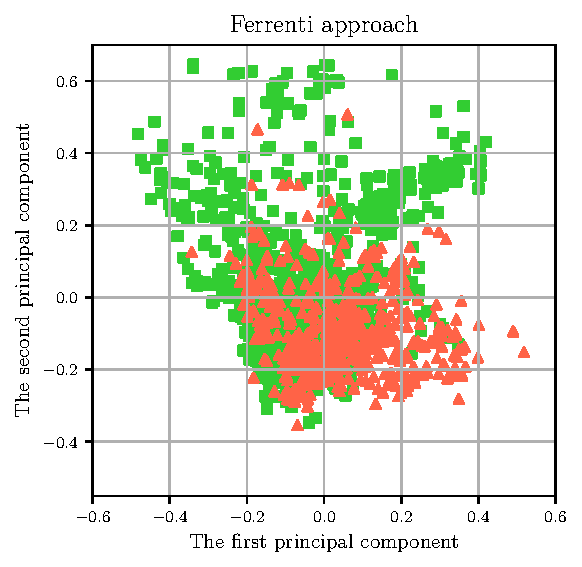
\includegraphics[width=1\textwidth]{figures/pca-2d-plots/01-ferrenti-approach.pdf}
    \end{subfigure}%
    \begin{subfigure}{0.3\textwidth}
        \centering
        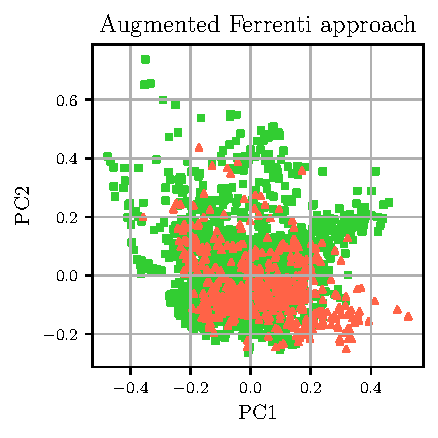
\includegraphics[width=1\textwidth]{figures/pca-2d-plots/02-augmented-ferrenti-approach.pdf}
    \end{subfigure}
    \begin{subfigure}{0.3\textwidth}
        \centering
        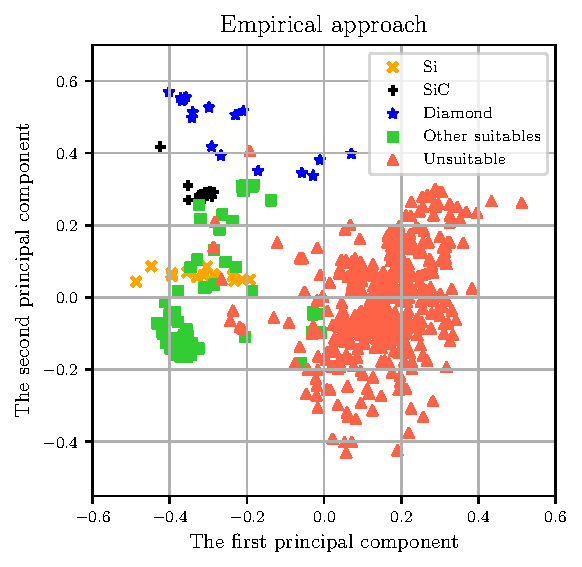
\includegraphics[width=1\textwidth]{figures/pca-2d-plots/03-insightful-approach.pdf}
    \end{subfigure}
    \vspace*{-95mm}
    \caption{Two-dimensional scatter plots for the three different approaches. We have identified the two eigenvectors corresponding to the two largest eigenvalues of the covariance-matrix, that is, the two most important principal components (PC1 and PC2) of the initial data from the Materials Project query. Then, we have transformed the three training sets resulting from the three approaches and visualized them as scatter plots. Green squares display suitable candidates and red triangles represent unsuitable candidates.}
    \label{fig:2dscatterplotpca}
\end{figure}

%\marianne{Return here to the basic issues with the two first approaches, in that they perhaps rely too much on practicalities. }  
It seems likely that the differences in Fig.~\ref{fig:2dscatterplotpca} can be attributed to the specific choices made when extracting data in each of the three approaches. Where the insightful approach takes advantage of the experimental knowledge that is already available in the literature, the Ferrenti and augmented Ferrenti schemes 
%procedures 
rely on assumptions of which material properties are responsible for the observed effect. 
An additional factor to consider is the use of practical considerations when restricting the parameter space for material choice. 
In short, a much clearer separation is observed for the insightful approach as compared to the others. 
These observations constitute an important finding of the work, as we show that it is possible to distinguish between suitable and unsuitable material candidates for QT. 
The manual approach of selecting suitable candidates based on experimental findings yields strong indication that a trend does exist and thus is possible to identify. 
Importantly, the presented methodology for selecting candidates as presented in the insightful approach can be adapted also to other material systems where a specific set of properties are desired but the specific mechanisms behind them are unknown. 


The constructed datasets encompass compounds formed by a plethora of combinations of surfaces, interfaces, nanostructures, compositions and structures. We note that this complexity is not necessarily reflected in the descriptors. 
%Additionally, we acknowledge that many compositions deemed as suitable candidates consist of either rare or dangerous elements. By utilizing an enormously large database as Materials Project, we have to account for their ultimate goal - to model all possible materials and their properties. 
%The automated process of adding an entry to their database does not necessarily contain all relevant information about a respective material. This is information that needs to be added manually.
Furthermore, we have utilized data obtained from high-throughput density functional theory calculations. Indeed, there are possible errors associated with every step, starting from an initial calculation, adding of data in the database, gathering of data, featurization of data, preprocessing of data, data mining, and finally training a model and making a prediction. Unfortunately, if an error has happened in the first part of the process, the error follows the entire process and will get increasingly harder to detect. Therefore, we are dependent on that the Materials Project has obtained data with high quality, and we note that it is likely that there are some errors present in our data sets.

\subsection*{Predicting Suitable Material Hosts for Quantum Technology}

Using the four algorithms, optimized at each of the three approaches, and applying them to the case of predicting materials as suitable material hosts for QT, yields 12 sets of results. In this chapter, we present sets of representative results for each approach. 

\subsubsection*{The Ferrenti Approach}
%Should we include materials in training set? Or keep it, but move into data mining discussion?
We first consider the machine learning classification of the test set based on the Ferrenti approach. 
Notably we find that carbon in diamond-like structure is classified as a suitable candidate from the training set in the Ferrenti approach. 
This is in agreement with the suitable candidates that were defined manually for the insightful approach. 
Interestingly, from the training set of the Ferrenti approach, we also find that carbon in two-dimensional graphite-like structures are labeled as suitable. 
%Out of the known suitable candidates defined for the insightful approach, we find carbon in diamond-like structures, but we also find two-dimensional carbon in graphite-like structures labeled as suitable. 
All structures of silicon are also labeled as suitable together with one entry of silicon carbide. 
Among other potentially suitable candidates we find ZnS, ZnSe, ZnO and ZnTe present. 

%\begin{figure}[t]
  \centering
  \begin{forest}
    for tree={l sep=1em, s sep=1em, anchor=center, inner sep=0.3em, fill=red!50, circle}
    [$23623$ compounds, node box, alias=bagging, above=1em
    [Logistic regression,node box,alias=a1
      [$11243$]
      [$12380$,fill=green!50,edge label={node[above=1ex,green arrow]{}}
      ]
    ]
    [Decision tree,node box,alias=a1
      [$12308$]
      [$11315$,fill=green!50,edge label={node[above=1ex,green arrow]{}}
      ]
    ]
    [Random forest,node box,alias=a1
      [$9345$]
      [$14278$,fill=green!50,edge label={node[above=1ex,green arrow]{}}
      ]
    ]
    [Gradient boost,node box,alias=a1
      [$11835$]
      [$11788$,fill=green!50,edge label={node[above=1ex,green arrow]{}}
      ]
    ]
    ]
  \end{forest}
\vspace*{-95mm}
\caption{Visualization of the predicted material candidates from the Ferrenti approach. The green nodes display the number of predicted suitable candidates while unsuitable ones are marked in red.}
\label{fig:01-predictions}
\end{figure}

%\begin{figure}[!ht]
  \centering
  \begin{forest}
    for tree={l sep=1em, s sep=1em, anchor=center, inner sep=0.3em, fill=red!50, circle}
    [$22550$ compounds, node box, alias=bagging, above=1em
    [Logistic regression,node box,alias=a1
      [$7557$]
      [$14993$,fill=green!50,edge label={node[above=1ex,green arrow]{}}
      ]
    ]
    [Decision tree,node box,alias=a1
      [$8143$]
      [$14407$,fill=green!50,edge label={node[above=1ex,green arrow]{}}
      ]
    ]
    [Random forest,node box,alias=a1
      [$7199$]
      [$15351$,fill=green!50,edge label={node[above=1ex,green arrow]{}}
      ]
    ]
    [Gradient boost,node box,alias=a1
      [$8762$]
      [$13788$,fill=green!50,edge label={node[above=1ex,green arrow]{}}
      ]
    ]
    ]
  \end{forest}
\vspace*{-95mm}
\caption{Visualization of the predicted material candidates from the augmented Ferrenti approach. The green nodes display the number of predicted suitable candidates while unsuitable ones are marked in red.} 
\label{fig:02-predictions}
\end{figure}
 
%\begin{figure}[!ht]
  \centering
  \begin{forest}
    for tree={l sep=1em, s sep=1em, anchor=center, inner sep=0.3em, fill=red!50, circle}
    [$24544$ compounds, node box, alias=bagging, above=1em
    [Logistic regression,node box,alias=a1
      [$23702$]
      [$842$,fill=green!50,edge label={node[above=1ex,green arrow]{}}
      ]
    ]
    [Decision tree,node box,alias=a1
      [$23347$]
      [$1197$,fill=green!50,edge label={node[above=1ex,green arrow]{}}
      ]
    ]
    [Random forest,node box,alias=a1
      [$24001$]
      [$543$,fill=green!50,edge label={node[above=1ex,green arrow]{}}
      ]
    ]
    [Gradient boost,node box,alias=a1
      [$23948$]
      [$596$,fill=green!50,edge label={node[above=1ex,green arrow]{}}
      ]
    ]
    ]
  \end{forest}
\vspace*{-95mm}
\caption{Visualization of the predicted material candidates from the insightful approach. The green nodes display the number of predicted suitable candidates while unsuitable ones are marked in red.} 
\label{fig:03-predictions}
\end{figure}


\begin{figure}[t]
    \centering
    (a) Ferrenti approach
    \\
    \begin{forest}
        for tree={l sep=1em, s sep=1em, anchor=center, inner sep=0.3em, fill=red!50, circle}
        [$23623$ compounds, node box, alias=bagging, above=1em
        [Logistic regression,node box,alias=a1
          [$11243$]
          [$12380$,fill=green!50,edge label={node[above=1ex,green arrow]{}}
          ]
        ]
        [Decision trees,node box,alias=a1
          [$12308$]
          [$11315$,fill=green!50,edge label={node[above=1ex,green arrow]{}}
          ]
        ]
        [Random forests,node box,alias=a1
          [$9345$]
          [$14278$,fill=green!50,edge label={node[above=1ex,green arrow]{}}
          ]
        ]
        [Gradient boosting,node box,alias=a1
          [$11835$]
          [$11788$,fill=green!50,edge label={node[above=1ex,green arrow]{}}
          ]
        ]
        ]
    \end{forest}
%\vspace*{-95mm}
    \\
    (b) Augmented Ferrenti approach 
    \\
\begin{forest}
    for tree={l sep=1em, s sep=1em, anchor=center, inner sep=0.3em, fill=red!50, circle}
    [$22550$ compounds, node box, alias=bagging, above=1em
    [Logistic regression,node box,alias=a1
      [$7557$]
      [$14993$,fill=green!50,edge label={node[above=1ex,green arrow]{}}
      ]
    ]
    [Decision trees,node box,alias=a1
      [$8143$]
      [$14407$,fill=green!50,edge label={node[above=1ex,green arrow]{}}
      ]
    ]
    [Random forests,node box,alias=a1
      [$7199$]
      [$15351$,fill=green!50,edge label={node[above=1ex,green arrow]{}}
      ]
    ]
    [Gradient boosting,node box,alias=a1
      [$8762$]
      [$13788$,fill=green!50,edge label={node[above=1ex,green arrow]{}}
      ]
    ]
    ]
  \end{forest}
%\vspace*{20mm}
    \\
    (c) Intuitive approach
    \\
 \begin{forest}
    for tree={l sep=1em, s sep=1em, anchor=center, inner sep=0.3em, fill=red!50, circle}
    [$24544$ compounds, node box, alias=bagging, above=1em
    [Logistic regression,node box,alias=a1
      [$23702$]
      [$842$,fill=green!50,edge label={node[above=1ex,green arrow]{}}
      ]
    ]
    [Decision trees,node box,alias=a1
      [$23347$]
      [$1197$,fill=green!50,edge label={node[above=1ex,green arrow]{}}
      ]
    ]
    [Random forests,node box,alias=a1
      [$24001$]
      [$543$,fill=green!50,edge label={node[above=1ex,green arrow]{}}
      ]
    ]
    [Gradient boosting,node box,alias=a1
      [$23948$]
      [$596$,fill=green!50,edge label={node[above=1ex,green arrow]{}}
      ]
    ]
    ]
  \end{forest}
%\vspace*{-95mm}
\caption{Visualization of the predicted material candidates from the (a) Ferrenti, (b) augmented Ferrenti and (c) intuitive approaches. Green and red nodes represent suitable and unsuitable candidates, respectively. }
\label{fig:predictions}
\end{figure}



The number of candidates predicted by each of the four machine learning algorithms 'Logistic regression', 'Decision tree', 'Random forest' and 'Gradient boost' is labeled in Figure~\ref{fig:predictions}(a) for the Ferrenti approach. 
From the training set of $23623$ materials, the four models consistently predict at least $11.000$ materials as promising candidates. All of the models agree on $6804$ suitable candidates, however, many of the materials are predicted with the probability similar to a coin-flip. 
If we were to raise the minimum bar of a prediction to
$0.7$ instead of $0.5$, the models would only agree on around $3000$ suitable candidates. 
Of the known suitable materials that were present in the training set, we find that all four models admit almost all materials with a chemical formula matching the known candidates. This can allow materials with unfortunate structures to be labeled as suitable candidates by all models. Consequently, the models do not recognize the strict band gap restriction, which makes it challenging to facilitate deep defects. Ideally, we would expect that the models would have probabilities lower than $0.5$ for all materials with band gaps lower than $0.5$~eV, which would be expected behavior based on the training set, but this is not the case. We find that many entries with band gaps lower than $0.5$~eV are predicted as both suitable and unsuitable candidates by all models. 

\subsubsection*{The augmented Ferrenti Approach}

%Should we include materials in training set? Or keep it, but move into data mining disc
%MB I think it's fine here also 
Next, we turn to the more liberal augmented Ferrenti approach. In the training set, we find a single entry for each of SiC, Si, GaN, ZnS, GaP, AlAs, AlP, carbon in both diamond- and graphite-like structures, and AlN in three different structures. The training set includes a larger variety of known suitable candidates compared to the Ferrenti approach due to admitting more elements in the initial restriction. However, since we also included a larger band gap restriction of $1.5$~eV, we find a more sparse representation of each known chemical formula present in the training set.

The four models predict at least $13.000$ materials as suitable candidates out of $22.550$ materials in the test set, where they all agree on a set of $9227$ predicted suitable candidates. Comparing to the training set reveals that all of the unlabeled known suitable candidates are, in fact, predicted as suitable candidates. Unfortunately, the models also yield predictions that do not match with what one would expect from physical considerations. 
All four machine learning models confidently predict NaCl as a suitable candidate, which we believe is unlikely due to the strong electrostatic interactions between Na and Cl. 
At least, single-photon emitters with sharp and bright zero-phonon lines are uncommon in materials with a strong ionic character. 
Furthermore, despite enforcing a larger band gap restriction of $1.5$~eV for the training set, we find that all models are predicting suitable candidates that exhibit band gaps substantially lower than $0.5$~eV.
Clearly, the models are not taking this important property into account when classifying the materials. 
 
\subsubsection*{The insightful approach}
The ML models that were trained on the data set defined from the insightful approach to data mining predict substantially fewer candidates as compared to the two other approaches. 
%Trained on the training set defined as the insightful approach, the models are able to predict radically fewer suitable candidates compared to the two latter approaches. 
A total of $842$, $1197$, $543$ and $596$ materials are classified as suitable candidates by logistic regression, decision tree, random forest and gradient boost, respectively. All the four ML models agree on a total of $214$ suitable candidates. However, $51$ of these have a band gap of $0.5$~eV or smaller as reported in Materials Project from PBE-level DFT calculations.  

%Cut down the amount of information given on perhaps not so suitable candidates, while rather emphasis the good predicted suitable candidates?

Initially, we consider the materials that were classified as suitable with a probability of $85 \ \%$ or higher by all the models; BN, CdSe, BC$_2$N, InAs, CuI, and ZnCd$_3$Se$_4$. 
The compound BN (mp-$1639$) is already present in the training data as a suitable candidate, and therefore we believe the models recognize this as a suitable candidate with high probability. Furthermore, two compositions of CdSe (mp-$2691$ and mp-$1070$) have been predicted as suitable, possibly as a consequence of CdS being present as a suitable candidate in the training set. The element S resides in the same group as Se, and the data shows that the two compounds of CdSe are associated with a calculated band gap of $0.5$ eV and $0.55$ eV, respectively, in the MP database. 
Comparing to experiment, high quality nanocrystals of CdS have been synthesized and studied for use as quantum dots since the nanocrystals emit in the visible range with a direct band gap of $2.5$~eV \cite{CelebiSerdar2007SaCo, BanerjeeR2000Eots}. %Unfortunately, Cd is a toxic metal which could make large scale fabrication challenging.  

We also find two compositions with the same chemical formula, the orthorhombic coordinated (mp-$629458$) and the chalcopyrite structured BC$_2$N (mp-$1008523$) where the first structure is in a polar space group while the latter is not. The band gaps are in MP calculated as $1.85$ eV and $1.65$ eV, respectively. BC$_2$N is known as heterodiamond and is a hybrid of diamond and BN. Both structures have, as expected, strong covalent character and have been studied for application as nanostructures \cite{Gao2017}, hydrogen storage \cite{Cai2017} and superhard materials \cite{Li2017, Jiang2020} in ab-initio calculations. Of similar compounds, it has been predicted that the diamond-like structure of BC$_3$N can be a prominent spin qubit material host \cite{Wang2020SpinQB}. By creating a boron (B) vacancy, it will immediately lead to an NV center with similar properties as found in the NV center in diamond. If this is also possible for BC$_2$N, remains to be seen. We note that BC$_3$N is not present in MP, and therefore not present in our dataset.

The compounds InAs (mp-$20305$), CuI (mp-$22895$ and mp-$569346$) and ZnCd$_3$Se$_4$ (mp-$1078597$) show some similar properties in the data, and have band gaps of $0.30$, $1.18$ and $1.73$~eV, respectively. Single self-assembled InAs quantum dots have already been demonstrated \cite{Liu2018}, and is therefore an exciting possible material to use in quantum technology. To the best of our knowledge, ZnCd$_3$Se$_4$ has yet to be synthesized and contains the toxic element Cd, which could prove an obstacle for large scale utilization. CuI, however, has recently been synthesized and was shown to exhibit remarkable optoelectronic properties \cite{Ahn2020}. Interestingly, the material exhibits a large ionic character with more similarities to other oxides in the dataset than, e.g., the more covalent materials of Si, SiC and diamond.  
It seems that ionic character alone is not an obstacle, but it is unknown at this time whether CuI has higher potential for hosting single-photon emitters, spin-manipulation or QT operation via nanostructuring. 
Note that NaCl was not predicted as suitable for QT in the insightful approach. 

Lowering the probability requirement from $85 \ \%$ to $75 \ \%$ for all models results in $66$ materials. 
The full list is contained in the Supplementary Material at \cite{supplementary}. 
The list of predicted suitable candidates now includes ternary compounds of the formula ABC$_2$. The elements Ga, Cd and Zn can occupy the A-site, Cu, Sn, Ag and Ge take the B-site, while S, Te, P or As may reside at the C site. Most of the formed compounds include toxic elements with one exception. This exception is ZnGeP$_2$ (mp-$4524$), which takes the chalcopyrite-like structure, with an indirect band gap of $1.2$~eV \cite{Zhang2015} as reported in the MP database and an experimentally reported band gap of $1.99$~eV \cite{Xing1989}.
ZnGeP$_2$ crystallizes in a non-polar space group, possesses no magnetic moment, has strong covalent bonds, and has been reported as an excellent mid-IR transparent crystal material that is suitable for nonlinear optical applications \cite{Zhang2015}. Importantly, it is possible to integrate sources of photon quantum states based on nonlinear optics with ZnGeP$_2$ \cite{Caspani2017}. 
We therefore identify ZnGeP$_2$ as an eligible candidate, but it remains unknown  
whether the candidate can facilitate the isolated deep energy levels often associated with defects showing quantum compatible properties. 
%if the candidate can provide isolation and shelter to experimentally facilitate a deep defect with quantum effects.

Among the $66$ materials that all models in the insightful approach agreed on with more than $75 \ \%$ probability, we emphasize the presence of Ge, GeC, BP and InP. Ge in the cubic structure (mp-$1198022$) shares many properties with Si and C in addition to the periodic column number. 
%In fact, the first transistors were made in germanium due to their appealing electrical properties, but silicon took over as the material of choice for microelectronics due to the outstanding quality of silicon dioxide. 
%, which allowed the fabrication and integration of increasingly smaller transistors \cite{Scappucci2020, Pillarisetty2011}. 
Ge has the highest hole mobility of semiconductors at room temperature, and is therefore considered a key material for the process of extending the chip performance in classical computers beyond the limits imposed by miniaturization  \cite{Scappucci2020}. Furthermore, like SiC, Ge can take advantage of the mature large-scale fabrication of silicon due to their similar properties. 
Similar considerations could be made for the case of GeC. 
Data from the Materials Project database suggests that the cubic compound GeC (mp-$1002164$) is a covalent material having a band gap of $1.8$~eV. 
Interestingly, as SiC is widely known as highly suitable host material for QT compatible defects, we encourage further research on GeC due to its comparable properties with SiC.

The compound BP (mp-$1479$ and mp-$1008559$) is present in our predictions in both the cubic and hexagonal structures. The indirect band gaps of the different structures are calculated at $1.46$~eV and $1.1$~eV, respectively, as reported in the MP database. They are both nonmagnetic and share several properties with the entries mentioned above; including ... The compound is non-toxic and has been synthesized with a potential for large-scale production \cite{MukhanovVladimirA2016Umso}.

Lastly, we will mention the prediction of InP (mp-$966800$) as a suitable candidate. The compound inhabits the hexagonal structure with corner-sharing InP$_4$ tetrahedra. InP is reported in the Materials Project to have a direct band gap of $0.51$~eV, and is considered as one of the most promising candidates 
to compete with 
Cd- or Pb- based QDs for, e.g., display and lighting applications \cite{Zhang2020a, Won2019}.

It is worth to mention that all models agree on several oxides being potential candidates when the probability cut-off is set low enough (but still above $50 \ \%$). However, we find that almost all the oxide compounds fall between the decision boundary defining suitable and unsuitable candidates, and none are present in the list defining the $66$ suitable candidates in the Supplementary Material. Due to the labeling of ZnO as a suitable candidate, we believe that the boundary was shifted sufficiently to admit several oxides as suitable candidates.
Removing ZnO from the training set for the insightful approach might result in fewer or even no oxide compounts being predicted above the suitability limit. 

The work of \citeauthor{Ferrenti2020} \cite{Ferrenti2020} suggests a list of $541$ viable hosts after the data mining procedure.  
Of these, we find only a single material present in our list of $66$ candidates (see the Supplementary Material at \cite{supplementary}). This material is the nontoxic compound MgSe (mp-$10760$) which crystallizes in the rock-salt structure. Its band gap is $1.98$~eV in the MP database with the experimental value being $5.6$~eV  \cite{SaumGeorge1959}. MgSe is notable for its available spin-zero isotopes in accordance with the criteria set by the of Ref.~\cite{Ferrenti2020}. We believe that these criteria favor defects acting as spin centers with qubit potential and MgSe is thus identified as a promising host material in this respect.  
%\oliver{Maybe also see if other compounds that were present in training set are present in their 541 hosts. }

%Supplementary information: List displaying the 66 predicted candidates that all models in the insightful approach agreed on with more than 75\% probability. %appendix/listof66materials

\subsubsection*{Comparison of the approaches}

Out of the three approaches, we find that the augmented Ferrenti approach is the least restricted approach and admits the most entries. The Ferrenti approach also admits a large number of entries, but is otherwise not very different from the augmented version. 
Importantly, by applying the four ML models to the data extracted using the two approaches, we are unable to reproduce the criteria the approaches are based on, such as band gap restriction or polar space group. Of course, the list of materials proposed by the Ferrenti and augmented Ferrenti approach is extensive, whereas the insightful approach predicts fewer suitable candidates where manually verification is achievable.  
Manual verification through a literature survey will often not be available, however, and perfecting automatic data mining and analysis is therefore an important goal of material informatics. 

It is important to note that the insightfull approach also proposed candidates with band gap energies lower than $0.5$~eV, but less compared to that of the other two approaches. Thus, all three approaches predicted suitable candidates with band gaps lower than the lowest in the training sets. 
%We believe there are three reasons for this.  
It is known that the GGA functional Materials Project applies is known to underestimate the band gap of many semiconductors. 
%underestimating the band gap severely, and therefore there is a chance that the models consider the band gap as noise and not useful information. 
It is therefore possible that the band gap is not considered an important parameter by the ML models. 
%Understanding the motivation behind the classification of the models will be an important step towards understanding ... 
Indeed, we did not find that the band gap was prominent in the principal components, although the band gap could be correlated with other more important features. 
Thus, one can argue that the models find other patterns that represent a better distinction between suitable and unsuitable candidates in the training sets, resulting in the band gap being redundant.

We find that $119$ of the $214$ candidates predicted as suitable by the insightful approach (when the probability cut-off is set to [X]) were also selected by all models in the augmented Ferrenti approach. 
%Of the $214$ suitable candidates predicted by all models in the insightful approach, we find $119$ of them also predicted as suitable by all models in the augmented Ferrenti approach. 
Similarly, $78$ of the $214$ are also predicted as suitable by all models in the Ferrenti approach. All approaches and their corresponding models agree on a $47$ potential candidates, where eight are elementary (unary), $29$ binary, and $10$ tertiary.
\textbf{The list of the $47$ materials agreed on by all models and all three approaches as suitable candidates with a probability $> X \ \%$ can be found in the Supplementary Material at \cite{supplementary}.} 


%\section*{Discussion} 
% Shorter section, includes summary, concluding remarks and is quite heavy on outlook.

%\oliver{The following paragraphs are "disclaimers" where we list possible pitfalls and weaknesses of this experiment. Could also be incorporated in the discussion instead?} MB I moved it up to data mining 

%SHORT SUMMARY FIRST HERE. 

%Motivated by our findings, we believe that further computational, experimental, or theoretical verification after a prediction of a possible promising material remains an important step in this work. This step is part of the workflow for novel materials discovery, which is visualized in \autoref{fig:ht-workflow}. Nevertheless, we have provided an exploratory analysis for the discovery of novel materials to be used in QT. Considering the number of materials predicted as suitable candidates by our models and approaches, we hope it encouragesfurther studies and identification of possible new material hosts. 

%We find that including toxic materials etc in the training set is vital for reliable predictions. They can then later be excluded when planning experiments, but the practical considerations should be saved for last and not included in the initial criteria.  

\section*{Methods}
%Should be rather short. Details can be included in a Supplementary Material. 

\subsection*{Information Flow}

\subsection*{Databases} %Sebastian and Oliver 
The Materials Project \cite{Jain2013, Jain2018} is an open-source project based on the Vienna Ab Initio Package (VASP) \cite{Kresse1996}. The Perdew-Burke-Ernzerhof \cite{Perdew1996} (PBE) functional is used to calculate band structures, while for transition metals, a $+U$ correction is applied to correct for correlation effects \cite{Wang2006}. The project is known as the initiator of materials genomics and offers a variety of calculated properties for over one hundred thousand inorganic crystalline materials, with frequent updates and extensions. 

The Open Quantum Materials Database (OQMD) \cite{Saal2013, Kirklin2015} contains thermodynamic and structural properties of more than 600.000 materials. The calculations are performed with the VASP software whereas the electron exchange and correlation are described with the PBE functional. The $+U$ extension is included for several calculations considering specific elements \cite{Stevanovic2012}. 

JARVIS-DFT \cite{Choudhary2020} is an open database based on the VASP software and consists of roughly 40.000 3D materials using the vdW-DF-OptB88 functional \cite{Thonhauser2007, Klimes2011}. Structures included in the database are originally taken from the Materials Project, and then re-optimized using the OPT-functional. Finally, the combination of the OPT and modified Becke-Johnson (mBJ) functionals is used to obtain a representative band gap of each structure \cite{Choudhary2018a}. 

The AFLOW \cite{Curtarolo2012, Curtarolo2012a, Calderon2015} repository is an automatic software framework for the calculations of a wide range of inorganic material properties. They utilize the PBE functional within VASP
%with projector-augmented wave (PAW) potentials 
to relax twice and optimize the ICSD-structure. 

AFLOW-ML \cite{Isayev2017} is an API that uses machine learning to predict thermo-mechanical and electronic properties based on the chemical composition and atomic structure alone, which they denote as \textit{fragment descriptors}. Initially, the API decides whether a given material is a metal or an insulator, where the latter is confirmed with an additional regression model to predict the band gap width. The accuracy is validated by a five-fold cross-validation process for each model, where they report a $93 \ \%$ prediction success of their initial binary classification model. 

Matminer \cite{Ward2018} is an open-source toolkit for material analysis written in Python. Matminer provides modules to extract information from a wide variety of databases. Additionally, they provide the tools to construct possibly thousands of features from calculations based on a material's composition, structure and electronic properties from DFT calculations, and have frameworks for visualization and automatic machine learning.

\subsection*{Material Informatics}  
Screening and workflow and approaches.  

\subsection*{Machine Learning} 

Machine learning  represents the science of giving computers the ability to learn without being explicitly programmed. The idea is that there exist generic algorithms which can be used to find patterns in a broad class of data sets without having to write code specifically for each problem. The algorithm builds its own logic based on the data. 

The approaches to ML are many, but are often split into two main categories, supervised and unsupervised. In supervised learning we know the answer to a problem, and let the computer deduce the logic behind it. On the other hand, unsupervised learning is a method for finding patterns and relationship in data sets without any prior knowledge of the system. Many researchers also operate with a third category, namely reinforcement learning. This is a paradigm of learning inspired by behavioral psychology, where learning is achieved by trial-and-error, solely from rewards and punishment. In this work our focus is on supervised learning only with labeled data. Our main focus is on classification problems.

In this work we have applied four well-known and tested machine learning methods for classification problems, these are (see for example \cite{Hastie2009,Mehta2019} for discussions and applications):
\begin{enumerate}
    \item Logistic regression,
    \item Decision trees,
    \item Random forests,
    \item Gradient boosting.
\end{enumerate}
Logistic regression \cite{Hastie2009} is a simple and frequently used method for binary and multi-category classification problems.  In addition to logistic regression, we have also applied and tested the predictions made by decision trees and ensemble methods like random forests and gradient boosting, the latter through the application of the computationally efficient  XGBoost library \cite{xgboost2016}. Gradient boosting and random forests use decision trees as weak learners and improve their predictability, through either collections of randomized decision trees (a subset of the features in the data sets are selected randomly en building a decision tree for classification)  in random forests or by using a decision tree as a weak learner and improve upon this model by iterative process that involves the estimation of the gradients of the cost/loss function \cite{Hastie2009}. Pure decision trees can easily lead to overfitting of the data under
 study, leading to a model that exhibits a high variance. Ensemble methods like random forests and gradient boosting on the other hand tend to soften the overfitting problem, resulting in both a small bias and a reduced variance of the model employed, see for example Ref.~\cite{Mehta2019} for an in-depth discussion of the bias-variance trade-off in machine learning applied to physics problems. Gradient boosting implemented through the  XGBoost library, is used widely by data scientists to achieve state-of-the-art results on many machine learning challenges.

\section*{Data availability} 
%We can put something else, standard text 
%The data that support the plots within this paper and other findings of this study are available from the corresponding authors upon reasonable request. [Marianne: I assume you want to add the Github link here?] 

The data that support the findings of this study are available from the corresponding author, and the datasets used to generate the ML models are available online at [Github link]. 

\section*{Code availability} 
%The codes developed in this study are available from the authors upon reasonable request. [Marianne: I assume you want to add the Github link here?] 
The codes employed to develop the ML models are available online at [Github link]. 

\bibliography{apssamp}% Produces the bibliography via BibTeX.

\begin{acknowledgments}

The work of MHJ is supported by the U.S. Department of Energy,
Office of Science, office of Nuclear Physics under grant
No. DE-SC0021152 and U.S. National Science Foundation Grants
No. PHY-1404159 and PHY-2013047. 
The work of MEB and LV was supported by the Research Council of Norway and the University of Oslo through the frontier research project FUNDAMeNT (no. 251131, FriPro ToppForsk-program). 
%Some of the computations were performed on resources provided by UNINETT Sigma2 - the National Infrastructure for High Performance Computing and Data Storage in Norway.  
The work of MEB was supported by an ETH Zurich Postdoctoral Fellowship. 

\end{acknowledgments}

%\section*{Author contributions} 
%Copied in from another paper 
%S.-M.J. conceived the idea and developed the simulation model. T.H.L. performed computer simulation. S.Y.B. and S.D.H. fabricated devices. D.-W.S., S.L., H.W.C. and J.-W.J. supported measurement of device performances. Y.-H.S. and X.-B.F. synthesised QD materials. S.Z. and J.Y. supported experiments. C.S. and Y.K. supported computer simulation. L.G.O. and G.A. supported data analysis. J.M.K. guided this work. S.-M.J., T.H.L. and S.Y.B. contributed equally. All the authors contributed to the preparation of the manuscript.

\section*{Competing interests}
The authors declare no competing interests.


\end{document}

